\documentclass{article}
\usepackage{arxiv} 

\usepackage[quiet]{fontspec} % Suppress font warnings
\usepackage{amsmath}
\usepackage{amsfonts}
\usepackage{amssymb}
\usepackage{dsfont} % For doublestroke 1
\usepackage[scr=dutchcal, scrscaled=1.05]{mathalfa} % Adds \mathscr
\usepackage{bm}
% Remove phoenician package as it conflicts with Persian text
% \usepackage{phoenician}
\usepackage{wrapfig}
\usepackage{anyfontsize}
\usepackage{mathtools}
\usepackage{graphicx}
\usepackage{float}
\usepackage{marginnote}
\renewcommand*{\marginfont}{\color{darkgray}\small}
\usepackage{wrapfig}
\usepackage{sidecap}
\usepackage[font=small]{caption}
\usepackage[font=small]{subcaption}
\usepackage{booktabs}
\usepackage{makecell} % Multi-line cells in tabular
\usepackage{diagbox}
\usepackage{multirow}
\newcounter{magicrownumbers}
\usepackage{pdflscape}
\usepackage{enumitem}
\setlist[description]{
	labelwidth=0pt,
	leftmargin=35pt,
	itemindent=-20pt,
	font=\normalfont\bfseries\rule[2.2pt]{2pt}{2pt}\space
}
\usepackage[table]{xcolor}
\usepackage{tikz}
\usetikzlibrary{arrows, calc, positioning}
\usepackage{tikz-cd}
\tikzcdset{every label/.append style = {font = \small}}
\usepackage{nicefrac}
\usepackage{accents}
\usepackage{afterpage}
\usepackage{etoc}
\usepackage[numbers]{natbib}
\usepackage[amsmath,thmmarks,thref]{ntheorem} % Removed hyperref from here

% Load custom commands BEFORE other packages that might use them
\usepackage{custom_commands}
% Fix for displaying Latin acronyms properly in Persian text
\newcommand{\CNN}{\lr{CNN}}
\newcommand{\cnn}{\lr{CNN}}
\newcommand{\mathfrakb}{\mathfrak{b}}
\newcommand\rownumber{\stepcounter{magicrownumbers}\arabic{magicrownumbers}}

% Patch for \listtheorems alignment
\makeatletter
\def\thm@@thmline@name#1#2#3#4{%
	\@dottedtocline{-2}{0em}{2.3em}%
	{\makebox[\widesttheorem][l]{#1 \protect\numberline{#2}}#3}%
	{#4}}
\@ifpackageloaded{hyperref}{%
	\def\thm@@thmline@name#1#2#3#4#5{%
		\ifx\\#5\\%
		\@dottedtocline{-2}{0em}{2.3em}%
		{\makebox[\widesttheorem][l]{#1 \protect\numberline{#2}}#3}%
		{#4}
		\else
		\ifHy@linktocpage\relax\relax
		\@dottedtocline{-2}{0em}{2.3em}%
		{\makebox[\widesttheorem][l]{#1 \protect\numberline{#2}}#3}%
		{\hyper@linkstart{link}{#5}{#4}\hyper@linkend}%
		\else
		\@dottedtocline{-2}{0em}{2.3em}%
		{\hyper@linkstart{link}{#5}%
			{\makebox[\widesttheorem][l]{#1 \protect\numberline{#2}}#3}\hyper@linkend}%
		{#4}%
		\fi
		\fi}
}
\makeatother

\newlength\widesttheorem
\AtBeginDocument{
	\settowidth{\widesttheorem}{گزاره ۱۰\quad}
}

% Theorem definitions
\theoremstyle{plain}
\theoremindent20pt
\theoremheaderfont{\normalfont\bfseries\hspace{-\theoremindent}}
\theoremseparator{.}
\theorembodyfont{\itshape}
\newtheorem{pro}{گزاره}[section]
\newtheorem{lem}[pro]{لم}
\newtheorem{cor}[pro]{نتیجه}
\newtheorem{thm}[pro]{قضیه}
\newtheorem{dfn}[pro]{تعریف}
\newtheorem{exa}[pro]{مثال}
\theoremstyle{nonumberplain}
\theoremheaderfont{\normalfont\upshape\hspace{-\theoremindent}} % Changed from \it to \upshape
\theoremseparator{:}
\theoremsymbol{$\Box$}
\newtheorem{proof}{اثبات}

% Table of contents utilities
\newcommand{\nocontentsline}[3]{}
\newcommand{\tocless}[2]{\bgroup\let\addcontentsline=\nocontentsline#1{#2}\egroup}
\newcommand{\toclesslab}[3]{\bgroup\let\addcontentsline=\nocontentsline#1{#2\label{#3}}\egroup}

\usepackage{sectsty}
\partfont{\fontsize{16.2}{19.2}\bfseries}
\renewcommand\part{%
	\markboth{}{}\secdef\@part\@spart
}

% Load hyperref AFTER xepersian
\usepackage[unicode]{hyperref}

% Load xepersian BEFORE other packages that might conflict
\usepackage{xepersian}
\settextfont{B Zar}
\setdigitfont{B Zar}

% Fallback for small caps
\newcommand{\fakesc}[1]{{\footnotesize #1}}

% Address Underfull \vbox
\raggedbottom

% Title and author - Fixed structure with proper Persian layout
\title{شبکه‌های کانولوشنی مستقل از مختصات \\ 
	\large کانولوشن‌های یکسان نسبت به ایزومتری و پیمانه روی منیفلدهای ریمانی}

\author{%
	موریس وایلر$^1$ \and
	پاتریک فوره$^1$ \and
	اریک ورلینده$^1$ \and
	مکس ولینگ$^{1,2}$
}

\date{
	\small
	$^1$دانشگاه آمستردام \\
	$^2$پژوهشگاه هوش مصنوعی کوالکام \\[1ex]
	\begin{tabular}{cc}
		\texttt{m.weiler.ml@gmail.com} & \texttt{p.d.forre@uva.nl} \\
		\texttt{e.p.verlinde@uva.nl} & \texttt{m.welling@uva.nl}
	\end{tabular}
}

\begin{document}
	
	\maketitle
	
	% Remove the complex author details section and use proper abstract
	% Abstract section
\begin{minipage}[t]{\textwidth}
	
	% chapters/00_abstract.tex
	\begin{abstract}
		
		انگیزه‌ای از موفقیت گسترده شبکه‌های عمیق کانولوشنی، علاقه زیادی برای تعمیم کانولوشن‌ها به منیفلدهای غیراقلیدسی وجود دارد.
		یک پیچیدگی عمده در مقایسه با فضاهای مسطح این است که مشخص نیست کرنل کانولوشن باید در کدام تراز روی یک منیفلولد اعمال شود.
		دلیل اساسی این ابهام آن است که منیفلولدهای عمومی دارای انتخاب متعارف چارچوب‌های مرجع (گیج) نیستند.
		بنابراین کرنل‌ها و ویژگی‌ها باید نسبت به \emph{مختصات دلخواه} بیان شوند.
		ما استدلال می‌کنیم که انتخاب خاص مختصات‌بندی نباید بر استنتاج شبکه تأثیر بگذارد -- آن باید \emph{مستقل از مختصات} باشد.
		تقاضای همزمان برای استقلال مختصات و اشتراک وزن منجر به الزامی روی شبکه می‌شود تا تحت تبدیل‌های گیج محلی (تغییرات چارچوب‌های مرجع محلی) \emph{تناوب‌پذیر} باشد.
		ابهام چارچوب‌های مرجع بدین‌گونه به $G$-\emph{ساختار} منیفلولد بستگی دارد،
		به طوری که سطح لازم تناوب‌پذیری گیج توسط \emph{گروه ساختار}~$G$ متناظر تجویز می‌شود.
		کانولوشن‌های مستقل از مختصات ثابت می‌شوند که نسبت به آن \emph{ایزومتری‌هایی} که تقارن‌های $G$-ساختار هستند تناوب‌پذیر باشند.
		نظریه حاصل به شکل آزاد از مختصات بر حسب بندل‌های فیبر فرمول‌بندی می‌شود.
		برای نمونه‌سازی طراحی کانولوشن‌های مستقل از مختصات، ما شبکه کانولوشنی روی نوار موبیوس پیاده‌سازی می‌کنیم.
		عمومیت فرمول‌بندی هندسه دیفرانسیل ما از شبکه‌های کانولوشنی با بررسی گسترده ادبیات نشان داده می‌شود
		که تعداد زیادی از شبکه‌های کانولوشنی اقلیدسی، شبکه‌های کانولوشنی کروی و شبکه‌های کانولوشنی روی سطوح عمومی را به عنوان نمونه‌های خاص کانولوشن‌های مستقل از مختصات توضیح می‌دهد.
		
		\begin{figure}[H]
			\centering
			\vspace*{2.5ex}
			\includegraphics[width=.94\columnwidth]{figures/mobius_conv_gauges.pdf}
			\caption{نمایش کانولوشن روی نوار موبیوس با گیج‌های مختلف}
		\end{figure}
	\end{abstract}
	
	% hack to keep abstract on front page, even though it overflows
	\vspace*{-20ex}
	
\end{minipage}
	
	\newpage
	
	%!TEX root=../GaugeCNNTheory.tex


\section{مقدمه}


\begin{figure}
	\centering
	\vspace*{-2ex}
	\includegraphics[width=.94\textwidth]{figures/satellite_kernels.pdf}
	\caption{\small
		ناظران مختلف A و B ممکن است یک الگوی ویژگی را از «نقطه دید» متفاوتی درک کنند.
		ماهواره‌ها در کاربرد ما، کرنل‌های کانولوشنی هستند که میدان دید محلی خود در اطراف~$p$ را در یک بردار ویژگی در~$p$ خلاصه می‌کنند.
		«نقطه دید» آن‌ها انتخابی از یک چارچوب مرجع محلی (گیج) در~p است که کرنل در امتداد آن هم‌تراز می‌شود.
		از آنجا که مشاهدات از هر دو نقطه دید یک الگوی یکسان را نشان می‌دهند، پاسخ‌های کرنل باید حاوی اطلاعات معادلی باشند، یعنی استنتاج باید \emph{مستقل از مختصات} باشد.
		این امر کرنل‌های کانولوشن را ملزم می‌کند که \emph{تحت تبدیلات گیج محلی هموردا} باشند، یعنی تغییرات چارچوب‌های مرجع.
		سطح هموردایی گیج توسط \emph{گروه ساختار}~$G$ تعیین می‌شود که هم به خمینه و هم به کاربرد بستگی دارد.
		{
			\color{gray}
			\scriptsize
			(مارمولک‌ها با مجوز \href{https://github.com/twitter/twemoji/blob/gh-pages/LICENSE-GRAPHICS}{\underline{\lr{Creative Commons Attribution 4.0 International}}} با تشکر از توییتر اقتباس شده‌اند.)
		}
	}
	\label{fig:satellite}
\end{figure}


در سال‌های اخیر، شبکه‌های عصبی عمیق به مدل‌های منتخب برای طیف گسترده‌ای از وظایف در یادگیری ماشین تبدیل شده‌اند.
موفقیت مدل‌های عمیق اغلب ریشه در طراحی خاص-وظیفه دارد که ساختار ریاضی داده‌های مورد پردازش را منعکس می‌کند.
یک مثال برجسته، شبکه‌های عصبی کانولوشنی (\CNN) هستند که از ساختار فضایی داده‌ها از طریق اتصال محلی و اشتراک‌گذاری وزن فضایی بهره‌برداری می‌کنند.
از آنجا که کرنل یکسانی در هر نقطه از فضا اعمال می‌شود، شبکه‌های کانولوشنی نسبت به انتقال هموردا هستند، به این معنی که الگوهای آموخته‌شده را به طور خودکار در سراسر موقعیت‌های مکانی تعمیم می‌دهند.
با توجه به موفقیت چشمگیر تجربی \CNN{}های اقلیدسی، علاقه زیادی به گسترش مدل‌های کانولوشنی برای پردازش سیگنال‌ها در دامنه‌های عمومی‌تر و هموردا ساختن آنها تحت گروه‌های تقارن بزرگ‌تر وجود دارد.


این کار به بررسی تعمیم شبکه‌های کانولوشنی به \emph{خمینه‌های ریمانی} می‌پردازد.
یک پیچیدگی عمده در تعمیم شبکه‌های کانولوشنی از فضاهای اقلیدسی $\R^d$ به خمینه‌های ریمانی عمومی این است که \emph{خمینه‌ها با انتخاب ارجحی از جهت مرجع همراه نیستند}، که بتوان یک کرنل کانولوشن را در امتداد آن برای اندازه‌گیری ویژگی‌ها هم‌تراز کرد.
از آنجا که هیچ جهت مرجعی ارجح نیست، کرنل باید به صورت \emph{دلخواه} روی خمینه هم‌تراز شود.
موضوع اصلی این کار، تنظیم این دل‌بخواهی بودن با مستقل ساختن استنتاج شبکه‌ها از هم‌ترازی خاص کرنل‌های کانولوشن است.
مشخص می‌شود که این امر نیازمند آن است که کرنل‌ها \emph{هموردای گیج} باشند، یعنی هموردا تحت تبدیلات هم‌ترازی کرنل.
پاسخ یک کرنل هموردای گیج هنگام تغییر هم‌ترازی‌اش به طور قابل پیش‌بینی تبدیل می‌شود
-- بنابراین تضمین می‌شود که محتوای اطلاعات استخراج‌شده برای هر انتخاب (دلخواه) هم‌ترازی یکسان باشد.


ما هم‌ترازی یک کرنل در نقطه‌ای~$p$ از یک خمینه $M$ را به عنوان انتخابی از یک \emph{چارچوب مرجع محلی} یا \emph{گیج} از فضای مماس متناظر $\TpM$ فرمول‌بندی می‌کنیم.
\emph{تبدیلات گیج} بنابراین تبدیلات بین انتخاب‌های چارچوب‌های مرجع هستند.
شکل~\ref{fig:intro_kernel_alignment_trivial} مفهوم هم‌تراز کردن کرنل‌ها در امتداد چارچوب‌های مرجع را به تصویر می‌کشد.
هم‌تراز کردن کرنل نسبت به \emph{میدان چارچوب} کانونی (که به طور منحصربه‌فرد ارجح است) صفحه اقلیدسی $\R^2$، همانطور که در بالا نشان داده شده، منجر به \emph{میدان کرنل} معمول \CNN{}های اقلیدسی می‌شود.
یک میدان چارچوب متفاوت، همانطور که در پایین نشان داده شده، به یک میدان کرنل جایگزین و در نتیجه یک شبکه جایگزین دلالت دارد.
همانطور که در بالا بیان شد، در بیشتر خمینه‌ها انتخاب چارچوب‌ها ذاتاً مبهم است به طوری که هیچ هم‌ترازی کرنل خاصی ارجح نیست.
شکل~\ref{fig:satellite} این موضوع را برای کره $S^2$ به تصویر می‌کشد، جایی که چارچوب‌ها تنها تا حد دوران‌ها منحصربه‌فرد هستند.


\begin{figure}[htbp]
	\centering
	% Arrange subfigures in a single row
	\begin{subfigure}[b]{0.22\textwidth}
		\centering
		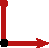
\includegraphics[width=0.8\linewidth]{figures/GpM_trivial.pdf}
		\caption{\small $G=\{e\}$}
		\label{fig:GpM_a}
	\end{subfigure}
	\hfill
	\begin{subfigure}[b]{0.22\textwidth}
		\centering
		\includegraphics[width=0.8\linewidth]{figures/GpM_reflect.pdf}
		\caption{\small $G=\Flip$}
		\label{fig:GpM_b}
	\end{subfigure}
	\hfill
	\begin{subfigure}[b]{0.22\textwidth}
		\centering
		\includegraphics[width=0.8\linewidth]{figures/GpM_SO2.pdf}
		\caption{\small $G=\SO2$}
		\label{fig:GpM_c}
	\end{subfigure}
	\hfill
	\begin{subfigure}[b]{0.22\textwidth}
		\centering
		\includegraphics[width=0.8\linewidth]{figures/GpM_scale.pdf}
		\caption{\small $G=\Scale$}
		\label{fig:GpM_d}
	\end{subfigure}
	
	% Standard caption
	\caption{\small
		انتخاب چارچوب‌های مرجع یک فضای مماس $\TpM$ همیشه منحصربه‌فرد نیست.
		ساختار هندسی (ساختار $G$) یک خمینه، زیرمجموعه‌ای ارجح از چارچوب‌های مرجع را ایجاب می‌کند به طوری که تبدیلات گیج بین این چارچوب‌ها در گروه ساختار~$G\leq\GL{d}$ قرار می‌گیرند.
		شکل‌های~\ref{fig:GpM_a}، \ref{fig:GpM_b}، \ref{fig:GpM_c} و~\ref{fig:GpM_d}
		چنین زیرمجموعه‌هایی از چارچوب‌ها را به ترتیب برای گروه بدیهی $G=\{e\}$، گروه بازتاب $G=\Flip$، گروه دوران $G=\SO2$ و گروه مقیاس‌پذیری~$G=\Scale$ نشان می‌دهند.
		ویژگی‌ها اندازه‌گیری‌ها را نسبت به هر یک از چارچوب‌های متمایز کدگذاری می‌کنند.
		ضرایب عددی آن‌ها نسبت به چارچوب‌های مختلف، توسط عمل یک نمایش گروهی $\rho$ از~$G$ به هم مرتبط می‌شوند.
	}
	\label{fig:GpM_examples}
\end{figure}


سطح ابهام در انتخاب چارچوب‌های مرجع به \emph{ساختار هندسی} خمینه بستگی دارد.
چنین ساختاری اغلب امکان
\emph{رفع ابهام چارچوب‌های مرجع تا حد تبدیلات تقارنی معین} (تبدیلات گیج) را فراهم می‌کند؛ به شکل~\ref{fig:GpM_examples} مراجعه کنید.
این بیانیه با چند مثال بهتر توضیح داده می‌شود:
\begin{itemize}[leftmargin=1.2cm]
	\item[{\rule[2.2pt]{2pt}{2pt}}]
	یک \emph{خمینه هموار} خام هیچ ترجیحی در انتخاب چارچوب‌ها ندارد.
	تبدیلات گیج بین چارچوب‌های عمومی، نگاشت‌های خطی معکوس‌پذیر دلخواه هستند، یعنی مقادیری در \emph{گروه خطی عمومی} ${G=\GL{d}}$ می‌گیرند.
	\item[{\rule[2.2pt]{2pt}{2pt}}]
	یک \emph{جهت‌گیری} از خمینه امکان تمایز چارچوب‌های چپ‌گرد از راست‌گرد را فراهم می‌کند.
	تبدیلات گیج بین چارچوب‌های هر یک از دو دست، حافظ جهت‌گیری هستند، یعنی عناصری از ${G=\operatorname{GL}^+(d)}$ هستند (نگاشت‌های خطی معکوس‌پذیر با دترمینان مثبت).
	\item[{\rule[2.2pt]{2pt}{2pt}}]
	یک \emph{فرم حجم} امکان تمایز \emph{چارچوب‌های با حجم واحد} را فراهم می‌کند.
	در این صورت، تبدیلات گیج حافظ حجم هستند، یعنی مقادیری در \emph{گروه خطی ویژه} $G=\operatorname{SL}(d)$ می‌گیرند.
	\item[{\rule[2.2pt]{2pt}{2pt}}]
	\emph{ساختار متریک} یک خمینه ریمانی امکان اندازه‌گیری فواصل و زوایا را در فضاهای مماس فراهم می‌کند و بنابراین امکان تمایز \emph{چارچوب‌های متعامد} را می‌دهد.
	تبدیلات گیج بین چارچوب‌های متعامد، دوران‌ها و بازتاب‌ها در \emph{گروه متعامد} $G=\O{d}$ هستند.
	\item[{\rule[2.2pt]{2pt}{2pt}}]
	با هم، یک \emph{جهت‌گیری و متریک} به \emph{چارچوب‌های متعامد جهت‌دار} دلالت دارند.
	در این صورت، تبدیلات گیج فقط دوران‌ها در \emph{گروه متعامد ویژه} $G=\SO{d}$ هستند.
	\item[{\rule[2.2pt]{2pt}{2pt}}]
	یک \emph{میدان چارچوب} روی خمینه شامل یک \emph{چارچوب منحصربه‌فرد} در هر نقطه از خمینه است.
	در این حالت، تبدیلات گیج بدیهی هستند که توسط \emph{گروه بدیهی} $G=\{e\}$ توصیف می‌شوند.
\end{itemize}
همه این ساختارهای هندسی مشترکاً یک زیرمجموعه ارجح (زیربندل) از چارچوب‌ها را تعریف می‌کنند به طوری که تبدیلات گیج مقادیری در یک \emph{گروه ساختار}~$G\leq\GL{d}$ می‌گیرند.
برای تأکید بر نقش محوری گروه ساختار $G$، چنین ساختارهایی به عنوان $G$-\emph{ساختار}~$\GM$ نامیده می‌شوند.
مثال‌های بصری از $G$-ساختارها برای گروه‌های ساختار $G$ و خمینه‌های~$M$ مختلف در شکل~\ref{fig:G_structures_intro} آورده شده است.


از آنجا که انتخاب چارچوب‌های مرجع ذاتاً مبهم است، هر کمیت هندسی و عملیات شبکه باید به طور مساوی نسبت به چارچوب‌های دلخواه $G$-ساختار~$\GM$ قابل نمایش باشد، یعنی باید $\GM$-\emph{مستقل از مختصات} باشد.
بردارهای ویژگی بنابراین با یک \emph{نمایش گروهی} (عمل گروهی خطی) $\rho$ از گروه ساختار $G$ مرتبط هستند که قانون تبدیل آنها را تحت تبدیلات گیج (گذار‌های با مقدار $G$ بین چارچوب‌های مرجع) تعیین می‌کند.
انتخاب خاص نمایش گروهی، نوع هندسی یک میدان بردار ویژگی را تعیین می‌کند.
مثال‌های معمول شامل میدان‌های اسکالر، بردار یا تانسور هستند، با این حال، انواع میدان عمومی‌تری نیز در عمل استفاده می‌شوند.
شکل~\ref{fig:gauge_trafos} استقلال از مختصات کمیت‌های هندسی را در مثال شناخته‌شده بردارهای مماس به تصویر می‌کشد.


هر لایه شبکه ملزم به رعایت قوانین تبدیل ویژگی‌هاست، یعنی باید تضمین کند که خروجی‌هایش همانطور که انتظار می‌رود تبدیل می‌شوند.
به طور خاص برای کانولوشن‌ها، استقلال از مختصات $\GM$ ایجاب می‌کند که اعمال کرنل مشترک نسبت به چارچوب‌های مختلف $G$-ساختار در یک نقطه $p\in M$ باید \emph{پاسخ یکسانی را تا حد یک تبدیل گیج} برانگیزد.
ما نشان می‌دهیم که این امر نیازمند $G$-راهبری (هموردایی گیج، معادله~\eqref{eq:G-steerable_kernel_space}) کرنل‌های کانولوشن است.
به طور شهودی، می‌توان کرنل‌های $G$-راهبر را به عنوان اندازه‌گیری ویژگی‌ها به صورت \emph{نسبی} نسبت به چارچوب‌های مرجع تصور کرد، که این امر ضروری است زیرا هیچ انتخاب چارچوب، یعنی هم‌ترازی کرنل \emph{مطلق}، ارجح نیست.%
\footnote{
	به شباهت با \emph{اصل نسبیت خاص} انیشتین توجه کنید، که به جای چارچوب‌های $G$-ساختار، بر برابری چارچوب‌های لخت تکیه دارد.
}
مثال‌هایی از کرنل‌های $G$-راهبر برای گروه بازتاب $G=\Flip$ در شکل~\ref{fig:intro_steerable_kernel} نشان داده شده است.
شکل~\ref{fig:intro_kernel_alignment_reflect} اشتراک‌گذاری چنین کرنل‌هایی را نسبت به چارچوب‌های مختلف یک ساختار $\Flip$ به تصویر می‌کشد.
قید $\Flip$-راهبری نوعی تقارن را بر کرنل‌ها تحمیل می‌کند، به طوری که هم‌ترازی‌های مختلف واقعاً منجر به پاسخ‌هایی می‌شوند که دقیقاً با تبدیلات گیج $\rho(g)$ متفاوت هستند.
ما در ادامه کانولوشن‌های مستقل از مختصات $\GM$ را به عنوان \emph{کانولوشن‌های} $\GM$ مخفف می‌کنیم.


علاوه بر اعمال کرنل‌های \emph{هموردای گیج}، کانولوشن‌های $\GM$ ممکن است \emph{هموردای ایزومتری} باشند، به این معنی که با عمل ایزومتری‌ها بر روی میدان‌های ویژگی جابجا می‌شوند، همانطور که در شکل~\ref{fig:lizard_conv_egg_intro} نشان داده شده است.
فرض کنید $\phi \in \IsomM$ یک ایزومتری (تقارن) از خمینه~$M$ باشد.
یک شبکه عصبی دقیقاً زمانی نسبت به عمل این ایزومتری هموردا است که الگوها در هر نقطه $p\in M$ به همان روشی پردازش شوند که الگوها در~$\phi(p)$ پردازش می‌شوند.
بنابراین هموردایی ایزومتری یک شبکه در تناظر یک به یک با \emph{ناوردایی ایزومتری اتصال عصبی آن} (میدان کرنل) است؛ به شکل~\ref{fig:isom_invariant_kernel_field_intro} مراجعه کنید.
از آنجا که کانولوشن‌های ما کرنل‌ها را نسبت به چارچوب‌های (دلخواه) $G$-ساختار $\GM$ اعمال می‌کنند، تقارن‌های میدان کرنل با تقارن‌های $G$-ساختار منطبق هستند.
با نشان دادن \emph{تقارن‌های (حافظ فاصله) یک $G$-ساختار} $\GM$ با $\IsomGM \leq \IsomM$، این دلالت دارد که کانولوشن‌های ما دقیقاً $\IsomGM$-هموردا هستند.
شکل~\ref{fig:intro_invariant_kernel_fields_plane} این واقعیت را که $G$-ساختارها و میدان‌های کرنل متناظر تقارن‌های یکسانی دارند، به تصویر می‌کشد.
خواننده تشویق می‌شود که $G$-ساختارها را در شکل~\ref{fig:G_structures_intro} با توجه به تقارن‌هایشان و ویژگی‌های هموردایی ضمنی کانولوشن‌های $\GM$ متناظر بررسی کند.


طراحی شبکه‌های کانولوشنی مستقل از مختصات $\GM$ بر روی خمینه‌های ریمانی نیازمند انتخاب یک $G$-ساختار است که به ملاحظات متعددی بستگی دارد.
اولاً، انتخاب گروه ساختار~$G$ \emph{هموردایی گیج محلی} کانولوشن را تعیین می‌کند:
یک کرنل $G$-راهبر به طور خودکار الگوهای آموخته‌شده را بر روی تمام ژست‌های مرتبط با $G$ از الگوها تعمیم می‌دهد؛ به شکل~\ref{fig:intro_lizard} مراجعه کنید.
ثانیاً، انتخاب خاص $G$-ساختار \emph{هموردایی ایزومتری سراسری} کانولوشن را تعیین می‌کند.
در کاربردهای تصویربرداری پزشکی، الگوها اغلب در دوران‌ها، بازتاب‌ها و موقعیت‌های دلخواه رخ می‌دهند
-- بنابراین باید یک ساختار $\O{d}$ ناوردای $\IsomGM = \E{d}$ را روی $\R^d$ انتخاب کرد، مشابه ساختار $\SO2$ که در شکل~\ref{fig:G_structure_intro_g} نشان داده شده است.
تصاویری مانند عکس‌های پرتره یک محور عمودی متمایز دارند، با این حال، بازتاب‌ها حول این محور آمار تصویر را ناوردا می‌گذارند
-- این امر نیازمند یک ساختار $\Flip$ مانند شکل~\ref{fig:G_structure_intro_d} است.
علاوه بر چنین ملاحظات تقارنی، توجه به این نکته مهم است که هر خمینه‌ای (توپولوژی) ساختارهای $G$ \emph{هموار} را برای هر انتخاب گروه ساختار~$G$ نمی‌پذیرد.
یک مثال نوار موبیوس است که توپولوژی پیچ‌خورده آن (عدم جهت‌گیری) مانع از تخصیص هموار متغیر جهت‌گیری‌های چارچوب می‌شود.
بنابراین یک عملیات کانولوشن مستقل از مختصات \emph{هموار} بر روی نوار موبیوس \emph{لزوماً} بر کرنل‌های راهبر-بازتابی تکیه دارد.


این کار شامل یک \emph{مرور ادبیات} گسترده بر روی شبکه‌های کانولوشنی است که عمومیت نظریه ما را نشان می‌دهد.
این بخش انواع مختلفی از \CNN{}ها را در فضاهای اقلیدسی، \CNN{}های کروی و کانولوشن‌ها را بر روی سطوح عمومی (مانند مش‌های سطحی) پوشش می‌دهد.
ما انتخاب‌های خاص $G$-ساختارها را که به طور ضمنی توسط نویسندگان انجام شده است، با تحلیل ویژگی‌های هموردایی سراسری و محلی مدل‌هایشان شناسایی می‌کنیم.
جدول~\ref{tab:network_instantiations} یک نمای کلی از طبقه‌بندی حاصل از شبکه‌های کانولوشنی مستقل از مختصات $\GM$ ارائه می‌دهد.


برای ارائه یک مثال دقیق در مورد چگونگی نمونه‌سازی نظریه ما در عمل، ما پیاده‌سازی کانولوشن‌های $\GM$ را بر روی نوار موبیوس برای~$G=\Flip$ مورد بحث قرار می‌دهیم.
این شامل استخراج کرنل‌های راهبر-بازتابی برای انواع میدان مختلف (نمایش‌های گروهی) و ارزیابی تجربی هموردایی ایزومتری پیش‌بینی‌شده نظری است.
همانطور که انتظار می‌رود، کانولوشن‌های مستقل از مختصات $\GM$ از پیاده‌سازی وابسته به مختصات ساده بهتر عمل می‌کنند.
کد در آدرس \url{https://github.com/mauriceweiler/MobiusCNNs} موجود است.

یک فرمول‌بندی \emph{بدون مختصات} از نظریه ما در زبان \emph{بندل‌های فیبر} ابداع شده است.
$G$-ساختارها $\GM$ زیربندل‌های اصلی $G$ از بندل چارچوب $\FM$ بر روی~$M$ هستند.
میدان‌های ویژگی \emph{برش‌هایی} از \emph{بندل‌های بردار ویژگی مرتبط} با $G$ هستند.
گیج‌ها \emph{تسهیم‌های بندل محلی} هستند، در حالی که تبدیلات گیج نگاشت‌های گذار بین چنین تسهیم‌هایی هستند.
ایزومتری‌هایی که یک کانولوشن $\GM$ نسبت به آنها هموردا است، \emph{اتومورفیسم‌های بندل اصلی} از $G$-ساختار هستند.


\CNN{}های مستقل از مختصات ما تعمیم‌هایی از \emph{\CNN{}های راهبر}~\cite{Cohen2017-STEER,3d_steerableCNNs,Weiler2019_E2CNN,Cohen2019-generaltheory,lang2020WignerEckart} از فضاهای اقلیدسی (یا همگن) به خمینه‌های ریمانی هستند.
در حالی که \CNN{}های راهبر بر تبدیلات \emph{فعال و سراسری} میدان‌های ویژگی تمرکز دارند، \CNN{}های مستقل از مختصات تبدیلات \emph{غیرفعال و محلی} بین چارچوب‌های مرجع را در نظر می‌گیرند.%
\footnote{
	این شبیه به تغییر تمرکز از \emph{کوواریانس لورنتس سراسری} در \emph{نسبیت خاص} به \emph{کوواریانس لورنتس محلی} در \emph{نسبیت عام} است.
}
ما نسخه‌های اولیه‌ای از نظریه \CNN{}های مستقل از مختصات ("\CNN{}های هموردای گیج") را در کارهای قبلی~\cite{gaugeIco2019,deHaan2020meshCNNs} پیشنهاد کردیم.
برخلاف این انتشارات، کار حاضر نظریه را با جزئیات بسیار بیشتری توسعه می‌دهد، آن را بر حسب بندل‌های فیبر فرمول‌بندی می‌کند، هموردایی تحت عمل ایزومتری‌ها را اثبات می‌کند و یک مرور ادبیات ارائه می‌دهد.
	%!TEX root=../GaugeCNNTheory.tex


\newpage
\setcounter{tocdepth}{2} % Keep tableofcontents depth
\tableofcontents

~ % <<=== newline

این کار در قالب یک مقدمه، سه بخش اصلی و یک پیوست سازماندهی شده است.

بخش~\ref{part:local_theory} تلاش می‌کند شبکه‌های عصبی مستقل از مختصات را با زبانی آسان معرفی کند.
میدان‌های ویژگی و لایه‌های شبکه نسبت به \emph{مختصات محلی} (تسهیم‌های بندل) بیان می‌شوند.
\emph{استقلال مختصات} مورد نیاز، مستلزم آن است که ویژگی‌ها با یک \emph{قانون تبدیل} خاصی مرتبط باشند.
لایه‌های شبکه ملزم به تضمین رفتار تبدیل صحیح ویژگی‌ها هستند.

بخش~\ref{part:bundle_theory} نظریه شبکه‌های عصبی مستقل از مختصات را بر حسب \emph{بندل‌های فیبر} رسمی‌سازی می‌کند.
این امر امکان فرمول‌بندی \emph{سراسری و مستقل از مختصات} را فراهم می‌کند، که به ویژه هنگام بررسی تناوب‌پذیری ایزومتری شبکه‌ها مفید است.
تعاریف از بخش~\ref{part:local_theory} با بیان عملیات مستقل از مختصات در تسهیم‌های بندل محلی (مختصات) بازیابی می‌شوند.

بخش~\ref{part:literature_review} نظریه ما را در \emph{کارهای مرتبط} جای می‌دهد.
این بخش بررسی‌های مفصلی از معماری‌های شبکه کانولوشنی بر روی هندسه‌های مختلف ارائه می‌دهد و آن‌ها را به عنوان شبکه‌های کانولوشنی مستقل از مختصات فرمول‌بندی مجدد می‌کند.
برای تسهیل توسعه معماری‌های شبکه جدید، ما ویژگی‌های مربوط به هندسه‌های خاص را قبل از بررسی شبکه‌هایی که بر روی آن‌ها عمل می‌کنند، مورد بحث قرار می‌دهیم.

خواننده می‌تواند بخش~\ref{part:bundle_theory} را در مرحله اول نادیده بگیرد
فرمول‌بندی از بخش~\ref{part:local_theory} برای خواندن مرور ادبیات در بخش~\ref{part:literature_review} کاملاً کافی است.

مروری بر مفاهیم و نتایج اصلی کار ما در بخش~\ref{sec:visual_intro} زیر ارائه شده است.
این مرور از معادلات پرهیز می‌کند و بر شهود هندسی از طریق بصری‌سازی‌ها تکیه دارد.
امیدواریم این بخش به مخاطبان غیرتخصصی کمک کند تا ایده‌ای از محتوای کار ما به دست آورند.


\subsubsection*{مرور کلی جزئیات}


\paragraph{بخش~\ref{part:local_theory}:}

هدف بخش~\ref{sec:gauge_cnns_intro_local} ابداع فضاهای ویژگی مستقل از مختصات است.
به طور خاص، بخش~\ref{sec:21_main} \emph{گیج‌ها، تبدیل‌های گیج و $G$-ساختارها} را معرفی می‌کند.
گیج‌ها روشی رسمی برای بیان بردارهای مماس (مستقل از مختصات) و توابع روی فضاهای مماس نسبت به چارچوب‌های مرجع هستند.
تبدیل‌های گیج بین این عبارات مختصاتی در گیج‌های مختلف ترجمه می‌کنند.
بخش~\ref{sec:feature_fields} \emph{میدان‌های بردار ویژگی} مستقل از مختصات را معرفی می‌کند.
همانند مورد بردارهای مماس، ضرایب عددی بردارهای ویژگی هنگام انتقال بین چارچوب‌های مرجع تغییر می‌کنند.
قوانین تبدیل بردارهای ویژگی به ویژه \emph{انتقال موازی} آن‌ها و پیش‌برداری آن‌ها هنگام عمل توسط \emph{ایزومتری‌ها} را تعیین می‌کنند، که به ترتیب در بخش‌های~\ref{sec:transport_local} و~\ref{sec:isometries_local} توضیح داده شده‌اند.

بخش~\ref{sec:gauge_CNNs_local} \emph{شبکه‌های عصبی} را که بین میدان‌های ویژگی نگاشت می‌کنند، توسعه می‌دهد.
\emph{عملیات نقطه‌ای}، مانند جمع بایاس، کانولوشن‌های $1\times1$ و غیرخطی‌ها، در بخش~\ref{sec:pointwise_operations} مورد بحث قرار می‌گیرند.
بخش~\ref{sec:gauge_conv_main} بر روی \emph{کانولوشن‌ها} با کرنل‌های گسترده فضایی تمرکز می‌کند.
هر یک از این عملیات در ابتدا بدون فرض اشتراک وزن معرفی می‌شوند، یعنی به عنوان مثال، اجازه یک کرنل متفاوت در هر نقطه از منیفولد را می‌دهند.
این کرنل‌ها (یا بایاس‌ها یا غیرخطی‌ها) به هیچ وجه محدود نمی‌شوند.
با این حال، هنگام نیاز به اشتراک وزن فضایی، آن‌ها مجبور می‌شوند که تناوب‌پذیر گیج باشند زیرا تنها مقادیر تناوب‌پذیر می‌توانند به صورت مستقل از مختصات به اشتراک گذاشته شوند.
بخش~\ref{sec:gauge_conv_isom_equiv} یک اثبات مختصر از تناوب‌پذیری ایزومتری کانولوشن‌های $\GM$ را بر حسب عبارات مختصاتی محلی ارائه می‌دهد.
ایده اصلی در اینجا این است که ایزومتری‌ها را می‌توان به عنوان القاکننده تبدیل‌های گیج (تفسیر منفعل) در نظر گرفت، که با تناوب‌پذیری گیج کرنل‌ها توضیح داده می‌شود.

بخش~\ref{sec:mobius_conv} پیاده‌سازی \emph{کانولوشن‌های مستقل از جهت‌گیری بر روی نوار موبیوس} را توصیف می‌کند.
پس از بررسی هندسه نوار موبیوس در بخش~\ref{sec:mobius_geometry}، انواع مختلفی از میدان‌های ویژگی در بخش~\ref{sec:mobius_representations} تعریف می‌شوند.
بخش~\ref{sec:mobius_cnn_ops_analytical} بعدی، شبکه‌های کانولوشنی مستقل از جهت‌گیری را به صورت تحلیلی توصیف می‌کند.
به طور خاص، ما کرنل‌های کانولوشنی تناوب‌پذیر گیج، بایاس‌ها و غیرخطی‌ها را برای هر یک از انواع میدان استخراج می‌کنیم.
بخش~\ref{sec:mobius_experiment_main} با یک پیاده‌سازی و ارزیابی عددی مدل‌های مربوطه به پایان می‌رسد.


\paragraph{بخش~\ref{part:bundle_theory}:}

بخش~\ref{sec:bundles_fields} محتوای بخش~\ref{sec:gauge_cnns_intro_local} را بازتاب می‌دهد، با این حال، به صورت سراسری و بر حسب \emph{بندل‌های فیبر}.
مقدمه‌ای کلی بر بندل‌های فیبر در بخش~\ref{sec:fiber_bundles_general} ارائه شده است.
بخش‌های~\ref{sec:GL_associated_bundles} و~\ref{sec:G_associated_bundles} بندل مماس $\TM$، بندل چارچوب $\FM$، $G$-ساختارها $\GM$ و بندل‌های بردار ویژگی مرتبط با $G$ ($\A$) را معرفی می‌کنند.
میدان‌های ویژگی به صورت سراسری به عنوان برش‌هایی از بندل‌های بردار ویژگی تعریف می‌شوند.
\emph{تسهیم‌های بندل محلی} (گیج‌ها)، که در بخش~\ref{sec:bundle_trivializations} مورد بحث قرار گرفته‌اند، این بندل‌ها را در مختصات بیان می‌کنند و بدین ترتیب تعاریف ما از بخش~\ref{sec:gauge_cnns_intro_local} را بازیابی می‌کنند.
ما به طور خاص نشان می‌دهیم که چگونه تسهیم‌های محلی بندل‌های مختلف یکدیگر را القا می‌کنند، به طوری که تبدیل‌های گیج (نگاشت‌های انتقال) آن‌ها همگام‌سازی می‌شوند.
بخش~\ref{sec:bundle_transport} \emph{انتقال‌دهنده‌های موازی} در $G$-بندل‌ها را مورد بحث قرار می‌دهد.

بخش~\ref{sec:gauge_CNNs_global} شبکه‌های مستقل از مختصات از بخش~\ref{sec:gauge_CNNs_local} را بر حسب بندل‌های فیبر بازنویسی می‌کند.
کانولوشن‌های $1\times1$ در بخش~\ref{sec:onexone} به عنوان مورفیسم‌های مشخص بندل برداری $M$ توصیف می‌شوند.
به طور جایگزین، آن‌ها را می‌توان به عنوان برش‌هایی از یک بندل همومورفیسم مشاهده کرد.
بخش~\ref{sec:global_conv} \emph{میدان‌های کرنل مستقل از مختصات} و \emph{تبدیل‌های میدان کرنل} را معرفی می‌کند.
این عملیات مشابه کانولوشن‌های $\GM$ هستند اما نیازی به اشتراک وزن ندارند، یعنی ممکن است در هر مکان فضایی یک کرنل متفاوت اعمال کنند.
یک \emph{میدان کرنل کانولوشنی} $\GM$ با اشتراک یک کرنل $G$-استیریبل (تناوب‌پذیر گیج) منفرد در سراسر منیفولد ساخته می‌شود.
سپس \emph{کانولوشن‌های مستقل از مختصات} $\GM$ به عنوان تبدیل‌های میدان کرنل با میدان‌های کرنل $\GM$-کانولوشنی تعریف می‌شوند.
هنگام بیان فرمول‌بندی مستقل از مختصات کانولوشن‌های $\GM$ نسبت به تسهیم‌های محلی (گیج‌ها)، عبارات مختصاتی کانولوشن‌های $\GM$ را از بخش~\ref{sec:gauge_conv_main} بازیابی می‌کنیم.

\emph{تناوب‌پذیری ایزومتری} کانولوشن‌های $\GM$ در بخش~\ref{sec:isometry_intro} بررسی می‌شود.
پس از معرفی ایزومتری‌ها، بخش~\ref{sec:isom_background} \emph{عمل پیش‌برنده} آن‌ها را بر روی بندل‌های فیبر مورد بحث قرار می‌دهد.
این عمل نیز می‌تواند در تسهیم‌های محلی بیان شود، که منجر به فرمول‌بندی از بخش~\ref{sec:isometries_local} می‌شود.
بخش~\ref{sec:isometry_equivariance} عمل ایزومتری‌ها بر روی میدان‌های کرنل را تعریف می‌کند و ثابت می‌کند که \emph{تناوب‌پذیری ایزومتری یک تبدیل میدان کرنل، ناوردایی ایزومتری میدان کرنل آن را نتیجه می‌دهد و بالعکس}.
کانولوشن‌های $\GM$ ثابت شده‌اند که تحت عمل آن ایزومتری‌هایی که اتومورفیسم‌های بندلی (تقارن‌ها) از $G$-ساختار~$\GM$ هستند، تناوب‌پذیر می‌باشند.
بخش~\ref{sec:quotient_kernel_fields} میدان‌های کرنل ناوردا با ایزومتری را با جزئیات بیشتری بررسی می‌کند و ثابت می‌کند که آن‌ها معادل \emph{میدان‌های کرنل در فضاهای خارج‌قسمتی} از عمل ایزومتری هستند
-- به طور شهودی، میدان‌های کرنل ناوردا با ایزومتری ملزم به اشتراک کرنل‌ها بر روی مدارات ایزومتری هستند.
این نتیجه به ویژه دلالت دارد که تبدیل‌های میدان کرنل تناوب‌پذیر ایزومتری در \emph{فضاهای همگن} لزوماً کانولوشن‌های $\GM$ هستند.


\paragraph{بخش~\ref{part:literature_review}:}

بخش سوم این کار نشان می‌دهد که تعداد زیادی از شبکه‌های کانولوشنی از ادبیات را می‌توان به عنوان اعمال کانولوشن‌های $\GM$ برای انتخاب خاصی از $G$-ساختار و انواع میدان تفسیر کرد.
این بخش با بحثی کلی در مورد انتخاب‌های طراحی شبکه‌های کانولوشنی مستقل از مختصات آغاز می‌شود.
جدول~\ref{tab:network_instantiations} مروری و طبقه‌بندی از مدل‌های مورد بررسی را ارائه می‌دهد.
خواننده دعوت می‌شود که به $G$-ساختارهای بصری‌سازی شده در بخش~\ref{part:literature_review} نگاهی بیندازد زیرا اینها ایده شهودی در مورد ویژگی‌های کانولوشن‌های $\GM$ مربوطه ارائه می‌دهند.

\emph{شبکه‌های کانولوشنی اقلیدسی} که نه تنها تناوب‌پذیر ایزومتری هستند بلکه به طور کلی‌تر تحت عمل \emph{گروه‌های آفین} تناوب‌پذیر هستند، در بخش~\ref{sec:instantiations_euclidean} بررسی می‌شوند.
این مدل‌ها اساساً معادل \emph{شبکه‌های کانولوشنی استیریبل} در فضاهای \emph{برداری} اقلیدسی $\R^d$ \cite{Cohen2017-STEER,3d_steerableCNNs,Weiler2019_E2CNN} هستند.
بخش~\ref{sec:steerable_cnns_in_coords} شبکه‌های کانولوشنی استیریبل را بررسی می‌کند و ارتباط آن‌ها با کانولوشن‌های $\GM$ را مورد بحث قرار می‌دهد.
این رویکرد تا حدی نامطلوب است زیرا $\R^d$ با یک میدان چارچوب کانونی (ساختار $\{e\}$) همراه است، که به طور ضمنی توسط مدل‌های تناوب‌پذیر نادیده گرفته می‌شود.
بخش~\ref{sec:euclidean_geometry} رویکردی اصولی‌تر را در پیش می‌گیرد و فضاهای \emph{آفین} اقلیدسی $\Euc_d$ را تعریف می‌کند که دقیقاً با $G$-ساختارهایی مجهز شده‌اند که منجر به کانولوشن‌های $\GM$ تناوب‌پذیر $\Aff(G)$ می‌شوند.
کانولوشن‌های واقعی $\GM$ در بخش~\ref{sec:euclidean_affine_equiv} تعریف می‌شوند.
بخش~\ref{sec:euclidean_literature} شبکه‌های کانولوشنی اقلیدسی تناوب‌پذیر آفین را که در ادبیات یافت می‌شوند، بررسی می‌کند.
آن‌ها عمدتاً در انتخاب‌های مفروض گروه‌های ساختار و نمایش‌های گروهی متفاوت هستند.

بخش~\ref{sec:instantiations_euclidean_polar} شبکه‌های کانولوشنی را در \emph{فضاهای اقلیدسی سوراخ‌دار} $\Euc_d\backslash\{0\}$، که مبدأ $\{0\}$ آن‌ها حذف شده است، پوشش می‌دهد.
این مدل‌ها نسبت به چرخش حول مبدأ تناوب‌پذیر هستند، با این حال، نسبت به انتقال تناوب‌پذیر نیستند.
آن‌ها بر اساس $G$-ساختارهایی هستند که با مختصات قطبی، مختصات لگاریتمی-قطبی یا مختصات کروی مطابقت دارند.

\emph{شبکه‌های کانولوشنی کروی} در بخش~\ref{sec:instantiations_spherical} پوشش داده می‌شوند.
بخش~\ref{sec:sphere_geometry} هندسه ۲-کره (جاسازی شده)~$S^2$ را مورد بحث قرار می‌دهد.
با تفسیر فضاهای مماس به عنوان زیرفضاهای دو بعدی یک فضای جاسازی~$\R^3$، عبارات فرم بسته نگاشت‌های نمایی و لگاریتمی، چارچوب‌ها، گیج‌ها، انتقال‌دهنده‌ها و عمل ایزومتری را استخراج می‌کنیم.
بخش~\ref{sec:spherical_CNNs_fully_equivariant} شبکه‌های کانولوشنی کروی تناوب‌پذیر $\SO{3}$ و $\OO{3}$ را بررسی می‌کند.
ما به طور خاص ثابت می‌کنیم که نظریه ما فرمول‌بندی عمومی کانولوشن‌های کروی توسط کوهن و همکاران~\cite{Cohen2019-generaltheory} را به عنوان یک حالت خاص شامل می‌شود.
شبکه‌های کانولوشنی کروی که فقط نسبت به چرخش $\SO{2}$ حول یک محور ثابت تناوب‌پذیر هستند در بخش~\ref{sec:spherical_CNNs_azimuthal_equivariant} توصیف می‌شوند.
بخش~\ref{sec:spherical_CNNs_icosahedral} شبکه‌های کانولوشنی بیست‌وجهی را بررسی می‌کند.
بیست‌وجهی کره را تقریب می‌زند اما از وجوه محلی مسطح تشکیل شده است که امکان پیاده‌سازی کارآمد عملیات کانولوشن را فراهم می‌کند.

یک بررسی از شبکه‌های کانولوشنی بر روی \emph{سطوح دو بعدی عمومی} در بخش~\ref{sec:instantiations_mesh} یافت می‌شود.
بخش~\ref{sec:surfaces_geom_main} مقدمه‌ای کوتاه بر هندسه دیفرانسیل کلاسیک سطوح جاسازی شده و گسسته‌سازی آن‌ها بر حسب شبکه‌های مثلثی ارائه می‌دهد.
کانولوشن‌های سطحی در ادبیات به دو دسته طبقه‌بندی می‌شوند:
دسته اول، که در بخش~\ref{sec:so2_surface_conv} پوشش داده شده است، بر اساس کرنل‌های $G=\SO{2}$-استیریبل است.
این مدل‌ها مستقل از انتخاب خاص چارچوب متعامد راست‌گرد هستند.
بخش~\ref{sec:e_surface_conv} دسته دوم مدل‌ها را بررسی می‌کند که بر اساس کرنل‌های $\{e\}$-استیریبل، یعنی غیرتناوب‌پذیر هستند.
این مدل‌ها به صراحت بر انتخاب یک میدان چارچوب تکیه دارند.
بنابراین آن‌ها عمدتاً در روش‌های اکتشافی که برای تعیین چارچوب‌های مرجع استفاده می‌شوند، تفاوت دارند.
توجه داشته باشید که چنین مدل‌هایی لزوماً در منیفلدهای غیرقابل موازی‌سازی مانند کره‌های توپولوژیکی ناپیوسته هستند.


\paragraph{پیوست:}

پیوست شامل اطلاعات اضافی و اثبات‌های طولانی است.

گیج‌ها به صورت رسمی تخصیص فوری چارچوب‌های مرجع به فضاهای مماس را انجام می‌دهند اما به نقاط روی منیفولد به صورت مستقل از مختصات اشاره دارند.
یک جایگزین محبوب انتخاب \emph{چارت‌های مختصاتی} است که به اصطلاح \emph{پایه‌های مختصاتی} (پایه‌های هولونومیک) فضاهای مماس را القا می‌کنند.
پیوست~\ref{apx:coordinate_bases} مقدمه‌ای بر فرمالیسم چارت‌ها ارائه می‌دهد و آن را با فرمالیسم گیج کلی‌تر مرتبط می‌کند.

پیوست~\ref{apx:coord_indep_weight_sharing} درباره \emph{استقلال مختصات} کرنل‌ها و \emph{اشتراک وزن} در امتداد چارچوب‌های مرجع توضیح می‌دهد.
اشتراک وزن مستقل از مختصات $\GM$ فقط برای کرنل‌های $G$-استیریبل امکان‌پذیر است.

کانولوشن‌های $\GM$ با بیان میدان‌های ویژگی در مختصات نرمال ژئودزیک محاسبه می‌شوند، جایی که آن‌ها با کرنل‌های کانولوشنی $G$-استیریبل مطابقت داده می‌شوند.
این فرآیند شامل یک \emph{انتگرال‌گیری بر روی فضاهای مماس} است که در پیوست~\ref{apx:tangent_integral} توصیف شده است.


کوندور و تریودی~\cite{Kondor2018-GENERAL}، کوهن و همکاران~\cite{Cohen2019-generaltheory} و بکرز~\cite{bekkers2020bspline} نظریه‌های نسبتاً عمومی از \emph{کانولوشن‌ها بر روی فضاهای همگن} را پیشنهاد کردند. از آنجا که این مدل‌ها وزن‌ها را از طریق عمل یک گروه تقارنی به اشتراک می‌گذارند، آن‌ها بسیار شبیه به تبدیل‌های میدان کرنل تناوب‌پذیر ایزومتری ما از بخش‌های~\ref{sec:isometry_equivariance} و~\ref{sec:quotient_kernel_fields} هستند. پیوست~\ref{apx:homogeneous_conv} این مدل‌ها را بررسی می‌کند و توضیح می‌دهد که چگونه آن‌ها با کانولوشن‌های $\GM$ ما مرتبط هستند.


پیوست~\ref{apx:lifting_iso_proof} ثابت می‌کند که میدان‌های کرنل ناوردا با ایزومتری در منیفولد معادل میدان‌های کرنل در فضاهای خارج‌قسمتی از عمل ایزومتری هستند.
حالت خاص فضاهای همگن، که در آن‌ها تبدیل‌های میدان کرنل تناوب‌پذیر ایزومتری معادل کانولوشن‌های $\GM$ هستند، در پیوست~\ref{apx:homogeneous_equivalence_proof} پوشش داده شده است.
کانولوشن‌های کروی کوهن و همکاران~\cite{Cohen2019-generaltheory} در پیوست~\ref{apx:spherical_conv_main} ثابت شده‌اند که یک حالت خاص از کانولوشن‌های $\GM$ کروی ما هستند.
بنابراین هر شبکه کانولوشنی کروی که توسط نظریه آن‌ها پوشش داده می‌شود، توسط نظریه ما نیز توضیح داده می‌شود.

پیوست~\ref{apx:smoothness_kernel_field_trafo} تأکید می‌کند که تبدیل‌های میدان کرنل و کانولوشن‌های $\GM$ ما به خوبی تعریف شده‌اند اگر میدان کرنل هموار باشد و شامل کرنل‌های با پشتیبانی فشرده باشد.
"به خوبی تعریف شده" در اینجا به این معنی است که انتگرال‌ها وجود دارند و میدان‌های ویژگی حاصل هموار هستند.

در نهایت، پیوست~\ref{apx:regular_field_scalar_GM} استدلال می‌کند که میدان‌های ویژگی که مطابق با نمایش منظم گروه ساختار $G$ تبدیل می‌شوند، معادل میدان‌های اسکالر بر روی $G$-ساختار هستند.
این موضوع از آن جهت اهمیت دارد که برخی مدل‌ها، به ویژه کانولوشن‌های گروهی، این دیدگاه را اتخاذ می‌کنند.
	%!TEX root=../GaugeCNNTheory.tex


\newpage


\begin{figure}
	\centering
	\includegraphics[width=.93\columnwidth]{figures/intro_transport_ambiguity.pdf}
	\caption{\small
		شهودی در مورد ابهام ذاتی اشتراک وزن در منیفلدهایی.
		\ \ \emph{چپ:}
		یک تفسیر رایج از اشتراک وزن در صفحه، جابجایی یک کرنل در کل فضا است.
		از آنجا که انتقال موازی در فضاهای مسطح مستقل از مسیر است، این امر بدون ابهام است.
		\ \ \emph{وسط:}
		در فضاهای خمیده، مانند کره، انتقال موازی وابسته به مسیر است.
		مسیرهای مختلف منجر به کرنل‌هایی می‌شوند که نسبت به یکدیگر چرخانده شده‌اند.
		\ \ \emph{راست:}
		نوار موبیوس یک منیفولد غیرقابل جهت‌گیری است.
		بنابراین، مسیرهای مختلف می‌توانند منجر به کرنل‌هایی شوند که نسبت به یکدیگر بازتاب یافته‌اند.
		\ \ \emph{پایین:}
		ما ترازهای مختلف کرنل را با انتخاب‌های مختلف چارچوب‌های مرجع محلی از فضاهای مماس مربوطه رسمی‌سازی می‌کنیم.
		به خوبی شناخته شده است که هیچ انتخابی از چارچوب‌های مرجع (گیج) در منیفلدهای عمومی ارجح نیست.
		مختصات‌بندی‌های مختلف با تبدیل‌های گیج مرتبط هستند، که مقادیری در گروه ساختار $G$ منیفولد (گروه بدیهی $G=\{e\}$ برای صفحه، گروه چرخش $G=\SO{2}$ برای کره و گروه بازتاب $G = \Flip$ برای نوار موبیوس) می‌گیرند.
		شبکه‌های کانولوشنی مستقل از مختصات، ابهام چارچوب‌های مرجع را با اعمال کرنل‌های کانولوشنی $G$-استیریبل (تناوب‌پذیر گیج) برطرف می‌کنند.
	}
	\label{fig:weight_sharing_ambiguity}
\end{figure}


\section{مرور کلی و شهود بصری}
\label{sec:visual_intro}


فرمول‌بندی جبری شبکه‌های کانولوشنی مستقل از مختصات نیازمند آشنایی با نظریه گروه‌ها، نظریه نمایش‌ها و هندسه دیفرانسیل است که ممکن است برای مخاطبان غیرتخصصی مانعی ایجاد کند.
با این حال، بیشتر ساختارها و نتایج ما از نظر هندسی بسیار شهودی هستند و می‌توان آن‌ها را با چند مثال بصری توضیح داد.
این بخش تلاش می‌کند تا مروری کلی و شهود بصری در مورد شبکه‌های کانولوشنی مستقل از مختصات ارائه دهد.

بخش~\ref{sec:intro_overview_GM_conv} زیر، کانولوشن‌های مستقل از مختصات $\GM$ را در منیفلدهای ریمانی معرفی می‌کند.
تناوب‌پذیری آن‌ها تحت عمل ایزومتری‌ها در بخش~\ref{sec:intro_overview_isometry} مورد بحث قرار می‌گیرد.
بخش~\ref{sec:intro_overview_G_structure_choice} در مورد عواملی که بر انتخاب $G$-ساختار در طراحی شبکه‌های کانولوشنی مستقل از مختصات تأثیر می‌گذارند، توضیح می‌دهد.


\toclesslab\subsection{\textit{G}-ساختارها و کانولوشن‌های مستقل از مختصات \textit{GM}}{sec:intro_overview_GM_conv}
از آنجا که کانولوشن‌ها اساساً با خاصیت اشتراک وزن خود مشخص می‌شوند، یک سؤال اصلی در این کار این است:
\vspace*{-1ex}
\begin{center}\it
	چگونه باید کرنل‌های کانولوشن بر روی منیفلدهای ریمانی به اشتراک گذاشته شوند؟
	\footnote{
		این سؤال به طور کلی‌تر برای هر تابع قالب محلی، به عنوان مثال بایاس‌ها یا غیرخطی‌های نقطه‌ای نیز کاربرد دارد.
	}
\end{center}

%%%%%%%%%%%%%%%%%%%%%%%%%%%%%%%%%%%%%%%%%%%%%%%%%%%%%%%%%%%%%%%%%%%%%%%
%%%%%%%%%%%%%%%%%%%%%%%%%%%%%%%%%%%%%%%%%%%%%%%%%%%%%%%%%%%%%%%%%%%%%%%
\marginnote{} % somehow forces stuff on first page...
%%%%%%%%%%%%%%%%%%%%%%%%%%%%%%%%%%%%%%%%%%%%%%%%%%%%%%%%%%%%%%%%%%%%%%%
%%%%%%%%%%%%%%%%%%%%%%%%%%%%%%%%%%%%%%%%%%%%%%%%%%%%%%%%%%%%%%%%%%%%%%%


یک رویکرد رایج \marginnote{اشتراک وزن از طریق تقارن‌ها} به اشتراک گذاشتن وزن‌ها از طریق عمل یک گروه تقارنی از فضای زیرین است~\cite{Cohen2016-GCNN,Kondor2018-GENERAL}.
به عنوان مثال، شبکه‌های کانولوشنی سنتی وزن‌ها را با جابجایی کرنل‌ها روی صفحه به اشتراک می‌گذارند، در حالی که شبکه‌های کانولوشنی کروی وزن‌ها را با چرخش کرنل‌ها روی کره به اشتراک می‌گذارند.
برای به اشتراک گذاشتن یک کرنل در کل فضا، عمل گروه تقارنی باید \emph{متعدی} باشد.
از آنجا که این امر به طور کلی برای ایزومتری‌های منیفلدهای ریمانی صادق نیست، این استراتژی برای هدف ما رد می‌شود.


اشتراک وزن در فضاهای اقلیدسی اغلب به عنوان "جابجایی" یک کرنل در فضا در نظر گرفته می‌شود.
\marginnote{اشتراک وزن از طریق انتقال}
از آنجا که در فضاهای مسطح انتقال موازی مستقل از مسیر انتخاب شده است، این امر منجر به تراز بدون ابهام کرنل‌ها می‌شود؛ به شکل~\ref{fig:weight_sharing_ambiguity} (چپ) مراجعه کنید.
با این حال، در فضاهای خمیده یا غیرقابل جهت‌گیری، انتقال موازی \emph{وابسته به مسیر} می‌شود و بنابراین برای اشتراک وزن نامناسب است.
شکل~\ref{fig:weight_sharing_ambiguity} (وسط و راست) این مشکل را برای کره و نوار موبیوس مثال می‌زند، جایی که مسیرهای مختلف منجر به تراز متفاوتی از کرنل می‌شوند.


از آنجا که مفهوم "ترازهای کرنل" تا حدی مبهم است
\marginnote{اشتراک وزن در امتداد چارچوب‌ها}
ابتدا باید آن را از نظر ریاضی دقیق کنیم:

\begin{minipage}{\textwidth}
	\begin{center}\it
		ما انتخاب تراز کرنل در نقطه‌ای $p\in M$ \\
		را به عنوان انتخاب یک چارچوب مرجع محلی (گیج)
		از فضای مماس مربوطه $\TpM$ رسمی‌سازی می‌کنیم.
	\end{center}
\end{minipage}

یک چارچوب مرجع در $p\in M$ یک تاپل مرتب $[e_1,\, \dots,\, e_d]$ از $d := \dim(M)$ بردار مماس خطی مستقل $e_i \in \TpM$ است که به عنوان محورهای چارچوب نامیده می‌شوند.
از آنجا که چارچوب‌های مختلف در~$p$ با تبدیل‌های خطی مرتبط هستند، انتخاب‌های مختلف چارچوب‌ها با تغییر شکل‌های کرنل خطی مطابقت دارند.
شکل~\ref{fig:intro_kernel_alignment_trivial} دو انتخاب مختلف از میدان‌های چارچوب را در~$M = \R^2$ نشان می‌دهد.
به اشتراک گذاشتن یک کرنل کانولوشنی در امتداد این میدان‌های چارچوب منجر به \emph{میدان‌های کرنل} (کانولوشنی) مربوطه می‌شود.


شناسایی ترازهای کرنل با چارچوب‌های مرجع این سؤال را مطرح می‌کند:
\begin{center}\it
	انتخاب چارچوب‌های مرجع محلی بر روی یک منیفولد (ریمانی) تا چه حد مبهم است؟
\end{center}
همانطور که در ادامه توضیح داده می‌شود، ابهام چارچوب‌های مرجع توسط یک $G$-ساختار که منیفولد به آن مجهز است، تعیین می‌شود.


\begin{SCfigure}
	\centering
	\includegraphics[width=.62\textwidth]{figures/intro_kernel_alignment_trivial.pdf}
	\captionsetup{width=.9\textwidth}
	\caption{\small
		یک ویژگی کلیدی کانولوشن‌ها این است که آن‌ها \emph{وزن‌ها را} در سراسر منیفولد \emph{به اشتراک می‌گذارند}.
		ما تراز یک کرنل در $p\in M$ را با \emph{انتخاب یک چارچوب مرجع} – یا \emph{گیج} – از فضای مماس مربوطه~$\TpM$ شناسایی می‌کنیم.
		بنابراین \emph{میدان‌های چارچوب} مختلف دلالت بر \emph{میدان‌های کرنل} (کانولوشنی) متفاوتی دارند.
		\\[1ex]
		انتخاب چارچوب‌ها اغلب منحصر به فرد نیست.
		ابهام در این انتخاب با $G$-\emph{ساختارها} رسمی‌سازی می‌شود؛ به شکل~\ref{fig:G_structures_intro} مراجعه کنید.
		برای در نظر گرفتن اختیاری بودن چارچوب‌ها، کرنل‌ها ملزم می‌شوند که $G$-استیریبل (تناوب‌پذیر) باشند، همانطور که در اشکال~\ref{fig:intro_steerable_kernel} و~\ref{fig:intro_kernel_alignment_reflect} بصری‌سازی شده است.
		\\[0pt]
	}
	\label{fig:intro_kernel_alignment_trivial}
\end{SCfigure}


\subsubsection{\textit{G}-ساختارها}
\label{sec:visual_intro_GM_subsub}

فضای \emph{همه} چارچوب‌های ممکن $\TpM$ با عنوان~$\FpM$ نشان داده می‌شود.
\marginnote{بندل چارچوب $\FM$}
با هم، چارچوب‌های همه فضاهای مماس، \emph{بندل چارچوب}~$\FM$ را تشکیل می‌دهند؛ به شکل~\ref{fig:frame_bundle} مراجعه کنید.
هیچ انتخاب خاصی از چارچوب‌ها در $\FM$ بر روی یک منیفولد هموار "عریان" (بدون ساختار هندسی اضافی) ترجیح داده نمی‌شود، که ابهام تراز کرنل‌ها را حداکثری می‌کند.
برای رفع ابهام چارچوب‌ها و ترازهای کرنل، منیفولد باید با \emph{ساختار هندسی اضافی} مجهز شود.


یک منیفولد ریمانی با \emph{ساختار متریک} مجهز شده است.
\marginnote{ساختار متریک $\OM$}
با ارائه یک حاصل‌ضرب داخلی (متریک ریمانی) بر روی فضاهای مماس، این ساختار امکان شناسایی چارچوب‌های خاصی را می‌دهد که محورهای آن‌ها \emph{متعامد} با یکدیگر هستند.
\emph{تبدیل‌های گیج}، یعنی تبدیل‌ها بین انتخاب‌های چارچوب‌های مرجع (به اشکال~\ref{fig:intro_gauge_isom_induction} (چپ) و~\ref{fig:gauge_trafos} مراجعه کنید)، سپس مقادیری در \emph{گروه متعامد}~$\O{d}$ می‌گیرند.
در منیفلدهای ریمانی، تراز کرنل‌ها همیشه تا چرخش‌ها و بازتاب‌ها بدون ابهام است.


شبکه‌های کانولوشنی اقلیدسی کرنل‌های کانولوشن (و در نتیجه چارچوب‌ها) را تراز می‌کنند
\marginnote{$G$-ساختارها $\GM$}
موازی با یکدیگر همانطور که در شکل~\ref{fig:intro_kernel_alignment_trivial} (بالا) بصری‌سازی شده است.
شبکه‌های کانولوشنی کروی معمولاً ترازهای کرنل را تا چرخش‌ها بدون ابهام می‌کنند، یعنی آن‌ها یک دست‌پری ترجیحی از چارچوب‌های مرجع را فرض می‌کنند.
ساختار متریک به تنهایی برای توصیف این تنظیمات کافی نیست، که نشان می‌دهد این منیفلدهایی با \emph{ساختار هندسی اضافی علاوه بر ساختار متریک} مجهز شده‌اند.
ما پیشنهاد می‌کنیم که چارچوب ریاضی مناسب، $G$-\emph{ساختارها} است و فرض می‌کنیم:

\begin{minipage}{\textwidth}
	\begin{center}\it
		ابهام در انتخاب چارچوب‌های مرجع (و در نتیجه ترازهای کرنل) \\
		بر روی یک منیفولد $M$ با $G$-ساختار $\GM$ آن رسمی‌سازی می‌شود.
	\end{center}
\end{minipage}

$G$-ساختارها $\GM$ \emph{بندل‌هایی از چارچوب‌های مرجع متمایز} بر روی $M$ هستند به طوری که \emph{تبدیل‌های گیج} بین چارچوب‌های یک فضای مماس واحد، مقادیری در \emph{گروه ساختار}~${G\leq\GL{d}}$ می‌گیرند.
به طور شهودی، می‌توان مجموعه $\GpM$ چارچوب‌های $\TpM$ را "شبیه" $G$ دانست، با این حال، بدون یک مبدأ متمایز.%
\footnote{
	$\GpM$ یک \emph{فضای همگن اصلی} از~$G$ (یا $G$-torsor) است.
}


بندل چارچوب $\FM$ خود یک $G$-ساختار با~${G=\GL{d}}$ است، در حالی که بندل چارچوب‌های متعامد $\OM$ یک $G$-ساختار (ساختار متریک) با~${G=\O{d}}$ است.
شبکه‌های کانولوشنی اقلیدسی سنتی بر روی میدان چارچوب کانونی در $\R^d$ که در شکل~\ref{fig:G_structure_intro_a} نشان داده شده است، تکیه دارند که یک $G$-ساختار برای گروه بدیهی~${G=\{e\}}$ است.
شکل~\ref{fig:G_structures_intro} $G$-ساختارها را برای منیفلدهای بیشتر و گروه‌های ساختار دیگر بصری‌سازی می‌کند.
مروری بر گروه‌های ساختار رایج در جدول~\ref{tab:G_structures} در بخش~\ref{sec:local_G-structure_G-atlas} یافت می‌شود.


ما در ادامه همیشه منیفلدهای ریمانی را مجهز به یک $G$-ساختار اضافی در کنار ساختار متریک خود فرض خواهیم کرد.%
\footnote{
	$G$-ساختار باید با ساختار متریک سازگار باشد به این صورت که چارچوب‌های متمایز در $\GM$ زیرمجموعه‌ای از چارچوب‌های متعامد در $\OM$ باشند زمانی که $G<\O{d}$.
	به طور خاص برای $G=\O{d}$، $G$-ساختار $\GM$ با ساختار متریک $\OM$ منطبق است و اطلاعات هندسی اضافی را اضافه نمی‌کند.
}
انتخاب خاص $G$-ساختار خواص شبکه عصبی را تعیین می‌کند؛ ما در مورد این انتخاب در بخش~\ref{sec:intro_overview_G_structure_choice} زیر توضیح خواهیم داد.


%%%%%%%%%%%%%%%%%%%%%%%%%%%%%%%%%%%%%%%%%%%%%%%%%%%%%%%%%%%%%%%%%%%%%%%%%%%%%%%%%%%%%%%%%%%%%%%%%%%%%%%%%%
\afterpage{ % execute argument of this command *after* end of current page
	\clearpage % clear any pending floats
	%%%%%%%%%%%%%%%%%%%%%%%%%%%%%%%%%%%%%%%%%%%%%%%%%%%%%%%%%%%%%%%%%%%%%%%%%%%%%%%%%%%%%%%%%%%%%%%%%%%%%%%%%%
	\begin{figure}
		\centering
		\vspace*{-4.ex}
		% The following line is the most likely source of the error.
		% Check the file 'chapters/intro_fig_G-structures.tex' for unclosed braces.
		%!TEX root=../GaugeCNNTheory.tex


\begin{subfigure}[b]{0.26\textwidth}
    \centering
    \includegraphics[width=1.\textwidth]{figures/G_structure_R2_1_big.pdf}
    \captionsetup{format=hang}
    \caption{\small
        \,  $M = \R^2$,
        \,\ $G = \{e\}$
    }
    \label{fig:G_structure_intro_a}
\end{subfigure}
\hfill
\begin{subfigure}[b]{0.26\textwidth}
    \centering
    \includegraphics[width=1.\textwidth]{figures/G_structure_R2_5_big.pdf}
    \captionsetup{format=hang}
    \caption{\small
        \,  $M = \R^2$,
        \,\ $G = \{e\}$
    }
    \label{fig:G_structure_intro_b}
\end{subfigure}
\hfill
\begin{subfigure}[b]{0.26\textwidth}
    \centering
    \includegraphics[width=1.\textwidth]{figures/G_structure_R2_no_origin_SO2_intro.pdf}
    \captionsetup{format=hang}
    \caption{\small
        \,  $M = \R^2\backslash\{0\}$,
        \,\ $G = \{e\}$
    }
    \label{fig:G_structure_intro_c}
\end{subfigure}
\\[2ex]
% 
% 
% 
% 
\begin{subfigure}[b]{0.26\textwidth}
    \centering
    \includegraphics[width=1.\textwidth]{figures/G_structure_R2_3_big.pdf}
    \captionsetup{format=hang}
    \caption{\small
        \,  $M = \R^2$,
        \,\ $G = \Flip$
    }
    \label{fig:G_structure_intro_d}
\end{subfigure}
\hfill
\begin{subfigure}[b]{0.26\textwidth}
    \centering
    \includegraphics[width=1.\textwidth]{figures/G_structure_R2_6_big.pdf}
    \captionsetup{format=hang}
    \caption{\small
        \,  $M = \R^2$,
        \,\ $G = \Flip$
    }
    \label{fig:G_structure_intro_e}
\end{subfigure}
\hfill
\begin{subfigure}[b]{0.26\textwidth}
    \centering
    \includegraphics[width=1.\textwidth]{figures/G_structure_R2_no_origin_O2_intro.pdf}
    \captionsetup{format=hang}
    \caption{\small
        \,  $M = \R^2\backslash\{0\}$,
        \,\ $G = \Flip$
    }
    \label{fig:G_structure_intro_f}
\end{subfigure}
\\[2ex]
% 
% 
% 
% 
\begin{subfigure}[b]{0.26\textwidth}
    \centering
    \includegraphics[width=1.\textwidth]{figures/G_structure_R2_2_big.pdf}
    \captionsetup{format=hang}
    \caption{\small
        \,  $M = \R^2$,
        \,\ $G = \SO2$
    }
    \label{fig:G_structure_intro_g}
\end{subfigure}
\hfill
\begin{subfigure}[b]{0.26\textwidth}
    \centering
    \includegraphics[width=.95\textwidth]{figures/G_structure_S2_1.pdf}
    \vspace*{-2ex}
    \captionsetup{format=hang}
    \caption{\small
        \,  $M = S^2$,
        \,\ $G = \SO2$
    }
    \label{fig:G_structure_intro_h}
\end{subfigure}
\hfill
\begin{subfigure}[b]{0.26\textwidth}
    \centering
    \makebox[\textwidth][c]{ % center over-wide figure
    \includegraphics[width=1.12\textwidth]{figures/suzanne_SO2_structure.pdf}
    }
    \vspace*{-3.ex}
    \captionsetup{format=hang, width=1.1\textwidth}
    \caption{\small
        $M = \textup{``\href{https://en.wikipedia.org/wiki/Blender_(software)\#Suzanne}{Suzanne}''}$\!,
        \ $G = \SO2$
    }
    \label{fig:G_structure_intro_i}
\end{subfigure}
\\[2ex]
% 
% 
% 
% 
\begin{subfigure}[b]{0.26\textwidth}
    \centering
    \includegraphics[width=1.\textwidth]{figures/G_structure_R2_4_big.pdf}
    \captionsetup{format=hang}
    \caption{\small
        \,  $M = \R^2$,
        \,\ $G = \Scale$
    }
    \label{fig:G_structure_intro_j}
\end{subfigure}
\hfill
\begin{subfigure}[b]{0.26\textwidth}
    \centering
    \includegraphics[width=.95\textwidth]{figures/G_structure_S2_2.pdf}
    \vspace*{-2ex}
    \captionsetup{format=hang}
    \caption{\small
        \,  $M = S^2\backslash$poles,
        \,\ $G = \{e\}$
   }
    \label{fig:G_structure_intro_k}
\end{subfigure}
\hfill
\begin{subfigure}[b]{0.26\textwidth}
    \centering
    \makebox[\textwidth][c]{ % center over-wide figure
    \includegraphics[width=1.1\textwidth]{figures/Mobius_R_structure.pdf}
    }
    \vspace*{-3.ex}
    \captionsetup{format=hang}
    \caption{\small
        \,  $M = \textup{M\"obius}$,
        \,\ $G = \Flip$
    }
    \label{fig:G_structure_intro_l}
\end{subfigure}

		\vspace*{1.5ex}
		\captionsetup{width=1.1\textwidth}
		\caption{\small
			نمونه‌ای از $G$-ساختارها $\GM$ برای گروه‌های ساختار $G$ و منیفلدهای $M$ مختلف.
			گروه ساختار $G$ نشان می‌دهد که تبدیل‌های گیج چه مقادیری می‌توانند بگیرند، و بنابراین زیرمجموعه چارچوب‌های متمایز در هر نقطه~$p$ چقدر "بزرگ" است.
			شکل~\ref{fig:G_structure_intro_a} $\{e\}$-ساختار کانونی (میدان چارچوب) در~$\R^2$ را نشان می‌دهد که مربوط به شبکه‌های کانولوشنی اقلیدسی سنتی است.
			\mbox{$G$-ساختارها} در
			اشکال~\ref{fig:G_structure_intro_d}، \ref{fig:G_structure_intro_g} و~\ref{fig:G_structure_intro_j}
			به ترتیب با اضافه کردن چارچوب‌های بازتاب یافته ($G=\Flip$)، چرخانده شده ($G=\SO{2}$) و مقیاس شده ($G=\Scale$) ساخته می‌شوند.
			\GM-کانولوشن‌های مربوطه نه تنها نسبت به انتقال تناوب‌پذیر هستند بلکه تحت عمل گروه‌های آفین~$\Aff(G)$ نیز تناوب‌پذیر می‌باشند.
			\mbox{$G$-ساختارها} معمولاً منحصر به فرد نیستند.
			اشکال~\ref{fig:G_structure_intro_b} و~\ref{fig:G_structure_intro_e} \mbox{$G$-ساختارهای} جایگزین را در~$\R^2$ نشان می‌دهند (مربوط به یک متریک جایگزین که چارچوب‌های آن‌ها نسبت به آن متعامد هستند).
			آن‌ها ممکن است از نظر عملی مرتبط نباشند اما انعطاف‌پذیری چارچوب ما را نشان می‌دهند.
			$\{e\}$-ساختار در شکل~\ref{fig:G_structure_intro_c} مربوط به مختصات قطبی است.
			از آنجا که $G$-ساختارها باید پیوسته باشند، ما مبدأ~$0$ را که مختصات قطبی در آن تکین هستند، حذف کردیم.
			می‌توان بار دیگر یک $\Flip$-ساختار را با اضافه کردن چارچوب‌های بازتاب یافته همانطور که در شکل~\ref{fig:G_structure_intro_f} نشان داده شده است، تعریف کرد.
			این $G$-ساختارها کانولوشن‌ها را در $\R^2\backslash\{0\}$ مدل می‌کنند که نسبت به $\SO{2}$ و $\O{2}$ تناوب‌پذیر هستند اما نسبت به انتقال تناوب‌پذیر نیستند.
			شکل~\ref{fig:G_structure_intro_h} $\SO{2}$-ساختار معمول را در 2-کره (جاسازی شده)~$S^2$ نشان می‌دهد، که زیربنای شبکه‌های کانولوشنی کروی تناوب‌پذیر $\SO{3}$ است.
			یک انتخاب محبوب دیگر $\{e\}$-ساختار در شکل~\ref{fig:G_structure_intro_k} است که توسط مختصات کروی القا می‌شود.
			توجه داشته باشید که این $\{e\}$-ساختار در قطبین تکین خواهد بود، که بنابراین از آن حذف می‌شوند.
			کاهش‌های پیوسته (یعنی غیرتکین) گروه ساختار فراتر از~$\SO{2}$ در کره از نظر توپولوژیکی مسدود شده‌اند.
			بنابراین کرنل‌های $G$-استیریبل با $G\geq\SO{2}$ برای کانولوشن‌های پیوسته در کره‌های توپولوژیکی مانند مش در شکل~\ref{fig:G_structure_intro_i} کاملاً ضروری هستند.
			شکل~\ref{fig:G_structure_intro_l} یک $\Flip$-ساختار را در نوار موبیوس نشان می‌دهد.
			از آنجا که نوار موبیوس غیرقابل جهت‌گیری است، کاهش پیوسته گروه ساختار را فراتر از گروه بازتابی~$G=\Flip$ نمی‌پذیرد.
		}
		\label{fig:G_structures_intro}
	\end{figure}
	%%%%%%%%%%%%%%%%%%%%%%%%%%%%%%%%%%%%%%%%%%%%%%%%%%%%%%%%%%%%%%%%%%%%%%%%%%%%%%%%%%%%%%%%%%%%%%%%%%%%%%%%%%
	\thispagestyle{empty}
	\clearpage % force a page break
}
%%%%%%%%%%%%%%%%%%%%%%%%%%%%%%%%%%%%%%%%%%%%%%%%%%%%%%%%%%%%%%%%%%%%%%%%%%%%%%%%%%%%%%%%%%%%%%%%%%%%%%%%%%


\subsubsection{\textit{GM}-شبکه‌های مستقل از مختصات}
هدف ما
\marginnote{استقلال از مختصات $\GM$ (کوواریانس)}
طراحی شبکه‌های عصبی بر روی منیفلدهای ریمانی با یک $G$-ساختار اضافی است.
اگر گروه ساختار $G$ بدیهی نباشد، \emph{هیچ انتخاب کانونی از چارچوب‌های مرجع (گیج) وجود ندارد}.
با این حال، برای انجام محاسبات عددی، \emph{برخی} گیج، که کرنل‌ها و ویژگی‌ها نسبت به آن بیان می‌شوند، باید انتخاب شود.
از آنجا که این انتخاب ذاتاً دلخواه است، ما تقاضا می‌کنیم که استنتاج شبکه‌ها در نهایت نباید به آن وابسته باشد، یعنی ما نیاز داریم:
\begin{center}\it
	شبکه‌های عصبی بر روی یک منیفولد ریمانی با $G$-ساختار $\GM$ \\
	باید بر اساس عملیات "مستقل از مختصات $\GM$" باشند.
\end{center}
"استقلال از مختصات $\GM$" در اینجا به این معنی است که \emph{همه کمیت‌های هندسی و توابع بین آن‌ها باید به همان اندازه به خوبی در هر گیج قابل بیان باشند}، یعنی نسبت به هر انتخابی از چارچوب‌های مرجع $G$-ساختار.
حالت خاص ضرایب بردار مماس و تبدیل‌های گیج بین آن‌ها در شکل~\ref{fig:gauge_trafos} بصری‌سازی شده است.
شکل~\ref{sec:gauges_TpM_functions} مثالی از یک نگاشت خطی و نمایش مستقل از مختصات آن بر حسب ماتریس‌ها نسبت به چارچوب‌های مختلف را نشان می‌دهد.


توجه داشته باشید که نیاز به استقلال از مختصات $\GM$ کاملاً انعطاف‌پذیر است:
برای $G=\GL{d}$، ما $\GM=\FM$ را داریم و بنابراین حداکثر سطح استقلال از مختصات را.
در انتهای دیگر طیف گروه‌های ساختار، $G=\{e\}$ قرار دارد، که برای آن $\GM$ یک میدان چارچوب ثابت است و استقلال از مختصات $\GM$ به وابستگی صریح به مختصات کاهش می‌یابد.
آزادی انتخاب $G$-ساختارهای دلخواه امکان کنترل دقیق بر استقلال از مختصات شبکه‌ها را فراهم می‌کند،
که در عمل به طور گسترده‌ای متفاوت است؛ به عنوان مثال به جدول~\ref{tab:network_instantiations} در بخش~\ref{part:literature_review} مراجعه کنید.


شبکه‌های ما \emph{میدان‌های بردار ویژگی} را بر روی منیفولد پردازش می‌کنند.
\marginnote{میدان‌های بردار ویژگی مرتبط با $G$}
بردارهای ویژگی کمیت‌های هندسی \emph{مستقل از مختصات} هستند، مانند بردارهای مماس.
نسبت به یک چارچوب (گیج) انتخاب شده، آن‌ها را می‌توان با \emph{بردارهای ضریب عددی} نمایش داد.
نیاز به استقلال از مختصات $\GM$ ایجاب می‌کند که ضرایب عددی در گیج‌های مختلف، محتوای اطلاعاتی یکسانی را کدگذاری کنند.
این امر به طور طبیعی با مرتبط کردن ویژگی‌ها با یک نمایش گروهی~$\rho$ از گروه ساختار~$G$ حاصل می‌شود که قانون تبدیل ضرایب آن‌ها را تحت تبدیل‌های گیج تعیین می‌کند:
\begin{center}\it
	میدان‌های بردار ویژگی با یک نمایش $G$ ($\rho$) مرتبط هستند که \\
	قانون تبدیل ضرایب عددی آن‌ها را هنگام تبدیل بین چارچوب‌های مرجع مشخص می‌کند.
	\\[1ex]
	از نظر فنی، میدان‌های ویژگی برش‌هایی از بندل‌های بردار ویژگی مرتبط با $G$ هستند.
\end{center}
مثال‌های معمول میدان‌های اسکالر، میدان‌های بردار مماس یا سایر میدان‌های تانسور هستند، با این حال، هر قانون تبدیلی مجاز است و می‌تواند توسط کاربر انتخاب شود.
انتخاب‌های رایج دیگر برای~$\rho$ در زمینه یادگیری عمیق، نمایش‌های کاهش‌ناپذیر یا منظم هستند؛
مثال‌های بیشتر در جدول~\ref{tab:network_instantiations} در بخش~\ref{part:literature_review} فهرست شده‌اند.


ما می‌خواهیم تأکید کنیم که نیاز به استقلال از مختصات $\GM$ صرفاً یک \emph{شرط سازگاری} است، که تضمین می‌کند مشاهده‌گران مختلف (چارچوب‌ها) بر روی مشاهده هندسی مستقل از مختصات یکسانی توافق دارند.
این امر مجموعه توابع مجاز را به هیچ وجه محدود \emph{نمی‌کند}، بلکه فقط چگونگی ارتباط عبارات آن‌ها نسبت به چارچوب‌های مختلف را مشخص می‌کند.
به طور خاص، \emph{شبکه‌های عصبی مستقل از مختصات $\GM$ به طور کلی نیازی به تناوب‌پذیری گیج ندارند}.
نیاز به تناوب‌پذیری گیج زمانی مطرح می‌شود که اشتراک وزن و استقلال از مختصات به طور همزمان طلب شود، یعنی کانولوشن‌های مستقل از مختصات $\GM$ بر روی کرنل‌های تناوب‌پذیر گیج تکیه دارند.
	%!TEX root=../GaugeCNNTheory.tex

\mypart{مقدمه‌ای بر شبکه‌های کانولوشنی مستقل از مختصات}
\label{part:local_theory}

شبکه‌های کانولوشنی سلسله‌مراتبی از میدان‌های ویژگی را از یک سیگنال ورودی بر روی یک منیفولد استخراج می‌کنند.
ویژگی‌ها از طریق کرنل‌ها محاسبه می‌شوند، که برای شناسایی الگوهای فضایی مشخص در ویژگی‌های سطح پایین‌تر بهینه شده‌اند.
ما تقاضا می‌کنیم که این فرآیند استنتاج صرفاً بر اساس آرایش نسبی ویژگی‌ها باشد و مستقل از انتخاب خاص مختصات‌بندی باشد.
بنابراین ویژگی‌ها باید کمیت‌های هندسی مستقل از مختصات باشند، مشابه اسکالرها، بردارها یا تانسورها.
در حالی که چنین کمیت‌های هندسی مستقل از مختصات وجود دارند، یک پیاده‌سازی کامپیوتری (غیرنمادین) نیازمند آن است که آن‌ها بر حسب ضرایب عددی در \emph{برخی} گیج، یعنی نسبت به برخی انتخاب از چارچوب مرجع، بیان شوند.
انتخاب خاص مختصات بی‌اهمیت است -- این تنها یکی از چندین توصیف معادل است.
چارچوب ریاضی مناسب برای تنظیم چنین درجات آزادی اضافی، \emph{نظریه‌های گیج} هستند.
یک نظریه گیج، برابری گیج‌های مختلف را با مرتبط کردن سازگار آن‌ها با یکدیگر از طریق \emph{تبدیل‌های گیج} در نظر می‌گیرد.
میدان‌های ویژگی مستقل از مختصات بنابراین با یک قانون تبدیل خاص، یعنی یک عمل گروهی از گروه ساختار که توصیف می‌کند ویژگی‌ها چگونه تحت تبدیل‌های گیج تبدیل می‌شوند، مرتبط هستند.
هر لایه شبکه عصبی که چنین میدان‌های ویژگی را پردازش می‌کند، ملزم به رعایت قوانین تبدیل آن‌ها برای حفظ استقلال از مختصاتشان است.

هدف این بخش اول از کار ما، معرفی شبکه‌های کانولوشنی مستقل از مختصات با زبانی آسان است.
بنابراین، شهود هندسی و بصری‌سازی‌ها بر فرمالیسم ریاضی ترجیح داده می‌شوند.
یک تبیین رسمی‌تر از تعاریف و نتایج ارائه شده در بخش~\ref{part:bundle_theory} آورده شده است.

\etocsettocdepth{2}
\etocsettocstyle{}{} % from now on only local tocs
\localtableofcontents

\vspace*{2.ex}

بخش~\ref{sec:gauge_cnns_intro_local} گیج‌ها و تبدیل‌های گیج را معرفی می‌کند که بر اساس آن‌ها میدان‌های بردارهای ویژگی مستقل از مختصات تعریف می‌شوند.
شبکه‌های عصبی که بین چنین میدان‌های ویژگی نگاشت می‌کنند، در بخش~\ref{sec:gauge_CNNs_local} توسعه یافته‌اند.
بخش~\ref{sec:mobius_conv} یک نمونه پیاده‌سازی از میدان‌های ویژگی و لایه‌های شبکه را در نوار موبیوس ارائه می‌دهد.
	%!TEX root=../GaugeCNNTheory.tex


\section{Coordinate independent feature fields}
\label{sec:gauge_cnns_intro_local}

The feature spaces of coordinate independent neural networks are spaces of feature vector fields.
The goal of this section is to define such feature fields and their geometric properties.

\etocsettocdepth{3}
\etocsettocstyle{}{} % from now on only local tocs
\localtableofcontents

Feature vectors are in practice represented relative to some reference frame and are characterized by their transformation laws when transitioning between different frames.
Section~\ref{sec:21_main} begins therefore with a discussion of the coordinatization of tangent spaces.
In particular, Section~\ref{sec:gauges_gauge_trafos} introduces gauges and gauge transformations of the tangent spaces as a formal way of describing choices of local reference frames and transformations between them.
Section~\ref{sec:gauges_TpM_functions} explains how functions on tangent spaces are represented relative to different coordinatizations
-- this introduces the idea of coordinate independent mappings, which we use later to define coordinate independent network layers.
Section~\ref{sec:local_G-structure_G-atlas} defines $G$-structures and $G$-atlases.
Coordinate independent feature fields and their gauge transformations are introduced in Section~\ref{sec:feature_fields}.
While Section~\ref{sec:individual_fields} describes the construction of individual feature fields,
Section~\ref{sec:stacked_fields} defines full feature spaces, consisting of multiple independent feature fields.
Parallel transporters of feature vectors and their representation relative to different coordinatizations are introduced in Section~\ref{sec:transport_local}.
Section~\ref{sec:isometries_local} discusses isometries and their action on geometric quantities like tangent vectors and feature vectors.

	%!TEX root=../GaugeCNNTheory.tex


\subsection{گیج‌ها، تبدیل‌های گیج و \textit{$G$}-ساختارها}
\label{sec:21_main}


\subsubsection{فضاهای مماس و چارچوب‌های مرجع}
\label{sec:gauges_gauge_trafos}


یک منیفولد هموار \lr{d}-بعدی $M$ دارای یک فضای مماس $\TpM\cong\R^d$ متصل به هر نقطه $p\in M$ است. فضاهای مماس، فضاهای برداری \lr{d}-بعدی هستند، با این حال، برخلاف $\R^d$، آن‌ها به طور کلی با هیچ انتخاب ارجح چارچوب مرجع همراه نیستند. یک بردار مماس $v\in \TpM$ یک شی \emph{مستقل از مختصات} است و بنابراین بلافاصله به صورت عددی با یک تاپل مختصاتی $(v_1,\dots,v_d)\in\R^d$ نمایش داده نمی‌شود. به طور انتزاعی‌تر، هر فضای مماس $\TpM$ با~$\R^d$ هم‌ریخت است اما به طور کلی هیچ هم‌ریختی کانونی بین آن‌ها وجود ندارد. بنابراین هر دو فضا از نظر ساختاری معادل هستند اما به هیچ روش ارجح به یکدیگر شناسایی نمی‌شوند.


یک \emph{گیج} (تسهیم محلی بندل مماس) بر روی $U^A\subseteq M$ به عنوان مجموعه‌ای از نگاشت‌های خطی معکوس‌پذیر که به صورت هموار وابسته به موقعیت هستند، تعریف می‌شود:
\begin{align}\label{eq:gauge_definition}
	\psi_p^A:\TpM\to\R^d \,,\ \ p\in U^A \,,
\end{align}
که هم‌ریختی‌های فضای برداری گمشده بین $\TpM$ و $\R^d$ را مشخص می‌کند. همانطور که در شکل~\ref{fig:gauge_trafos} بصری‌سازی شده است، آن‌ها با تخصیص یک \emph{بردار ضریب} به فضاهای مماس مختصات می‌دهند:
\begin{align}
	v^A\ :=\ \psi_p^A(v) \ \in\R^d
\end{align}
به هر بردار مماس مستقل از مختصات $v\in \TpM$. معکوس این رابطه می‌دهد:
\begin{align}
	v\ =\ \left(\psi_p^A\right)^{-1}\! (v^A)
	\ =\ \left(\psi_p^A\right)^{-1}\!\! \left(\sum\nolimits_i v_i^A \epsilon_i\right)
	\ =\ \sum\nolimits_i v_i^A\, \left(\psi_p^A\right)^{-1}\!(\epsilon_i)
	\ =:\ \sum\nolimits_i v_i^A\, e_i^A \,,
\end{align}
که در آن $\{\epsilon_1,\dots,\epsilon_d\}$ را پایانه استاندارد $\R^d$ نامگذاری کرده‌ایم و از خطی بودن گیج برای بیرون کشیدن جمع استفاده کرده‌ایم. این نشان می‌دهد که گیج را می‌توان به عنوان مجهز کردن هر فضای مماس $\TpM$ با یک \emph{چارچوب مرجع} در نظر گرفت:
\begin{align}\label{eq:framefield_gauge_equivalence}
	\left[e^A_{1}, \,\dots,\, e^A_{d}\right]
	\ :=\ \Big[(\psi_p^A)^{-1}(\epsilon_1), \:\dots\,,\; (\psi_p^A)^{-1}(\epsilon_d)\Big] \,,
\end{align}
که به عنوان یک \lr{d}-تاپل از بردارهای مماس خطی مستقل تعریف می‌شود که با نگاشت پایه استاندارد $\R^d$ به عقب از طریق نگاشت معکوس گیج به دست می‌آید. برای اختصار، ما در ادامه از نماد کوتاه‌شده $\big[e_i^A \big]_{i=1}^d$ برای چارچوب‌ها $\big[e_1^A, \dots, e_d^A \big]$ استفاده خواهیم کرد. ضرایب $v^A$ مختصات $v$ نسبت به این چارچوب هستند. مجموعه‌ای از چارچوب‌های القا شده توسط $\psi_p^A$ بر روی $U^A$ (هموار) \emph{میدان چارچوب} نامیده می‌شود؛ برای بصری‌سازی به شکل~\ref{fig:gauge_trafos_manifold} مراجعه کنید.


\begin{figure}
	\centering
	\includegraphics[width=\columnwidth]{figures/gauges_TpM.pdf}
	\caption{\small
		شناسایی $\TpM\!\cong\!\R^2$ با $\R^2$ از طریق گیج‌های مختلف.
		یک بردار مماس (مستقل از مختصات) $v\in \TpM$ (نارنجی) را می‌توان به صورت عددی با یک تاپل مختصاتی $v^A=\psi_p^A(v)=\big(1,1\big)^\top$ نسبت به گیج $\psi_p^A$ (قرمز) یا، به طور معادل، با $v^B=\psi_p^B(v)=(\sqrt{2},0)^\top$ نسبت به گیج $\psi_p^B$ (سبز) نمایش داد.
		انتخاب یک گیج مربوط به انتخاب $[e_1^A,e_2^A]$ یا $[e_1^B,e_2^B]$ از چارچوب مرجع است.
		در یک منیفولد عمومی هیچ انتخابی از گیج یا مختصات‌بندی پیش‌فرض ارجح نیست.
		گیج‌های مختلف، و در نتیجه چارچوب‌های مرجع، با تبدیل‌های گیج $g_p^{BA}:=\psi_p^B\circ(\psi_p^A)^{-1}$ (آبی) مرتبط هستند که مقادیری در گروه ساختار $G$ تعریف شده می‌گیرند.
		این شکل تفسیری گرافیکی از نمودارهای جابجایی در معادله~\eqref{eq:commutative_diagram_TpM} و شکل~\ref{fig:trivialization_TM} است.
		توجه داشته باشید که گیج‌ها بلافاصله به فضاهای مماس مختصات می‌دهند.
		شکل~\ref{fig:affine_charts} در بخش~\ref{sec:euclidean_geometry} یک نمودار مشابه برای چارت‌های (آفین) را نشان می‌دهد که به منیفولد مختصات می‌دهند و بدین ترتیب گیج‌ها ("پایه‌های مختصات") را \emph{القا} می‌کنند.
	}
	\label{fig:gauge_trafos}
\end{figure}


گیج‌های $\psi^X$ فضاهای مماس را تنها در همسایگی‌های محلی $U^X\subseteq M$ مختصات می‌دهند، و به دلیل موانع توپولوژیکی به طور کلی نمی‌توانند به کل منیفولد بدون نقض فرض همواری گسترش یابند.
بنابراین یک \emph{اطلس} در نظر گرفته می‌شود:
\begin{align}
	\mathscr{A} \,=\, \big\{\! \big(U^X, \psi^X\big) \!\big\}_{X\in \mathfrak{X}} \,,
\end{align}
متشکل از گیج‌های هموار بر روی مجموعه‌ای از همسایگی‌های $U^X$ که منیفولد را پوشش می‌دهند، یعنی شرط $\bigcup_{X\in \mathfrak{X}} U^X = M$ را برآورده می‌کنند، که در آن $\mathfrak{X}$ یک مجموعه اندیس است.%
\footnote{
	اطلس گیج‌ها بسیار شبیه به اطلس‌های معمول چارت‌های یک منیفولد است (پیوست~\ref{apx:coordinate_bases}).
	تفاوت این است که اطلس‌های مورد نظر در اینجا مستقیماً به بندل مماس $\TM$ مختصات می‌دهند به جای منیفولد $M$.
}
در نواحی همپوشانی $U^A\cap U^B\neq\varnothing$ از همسایگی‌ها، گیج‌های مختلف $\psi_p^A$ و $\psi_p^B$ توسط \emph{توابع گذار} هموار به هم متصل می‌شوند:
\begin{align}\label{eq:transition_fct_local_def_21}
	g^{BA}\!:\, U^A\cap U^B\to\GL{d},\quad p \mapsto g_p^{BA} := \psi_p^B \circ \left(\psi_p^A\right)^{-1}.
\end{align}
در اینجا ما دامنه مشترک (فعلاً) را با \emph{گروه خطی عمومی} $\GL{d}$ در نظر می‌گیریم، متشکل از همه ماتریس‌های معکوس‌پذیر در $ \R^{d\times d}$، که رابطه بین هر جفت از هم‌ریختی‌های فضای برداری (گیج‌ها) یا چارچوب‌های مرجع را توضیح می‌دهند.
عمل چنین تابع گذاری بر روی یک گیج داده شده یک \emph{تبدیل گیج} را تعریف می‌کند:
\begin{align}\label{eq:gauge_trafo_local_def_21}
	\psi_p^B\ =\ g_p^{BA} \!\cdot \psi_p^A.
\end{align}
از نظر یک نمودار جابجایی، رابطه بین گیج‌های مختلف به صورت زیر بصری‌سازی می‌شود:%
\footnote{
	\mbox{
		\emph{نمودارها} یک نمای کلی بصری از توابع و فضاهایی را که بین آن‌ها نگاشت می‌کنند، ارائه می‌دهند.
		به عنوان مثال، نمودار
	}
	\begin{minipage}{.2\textwidth}
		${
			\mkern30mu
			\begin{tikzcd}[column sep=30pt, row sep=8pt, ampersand replacement=\&]
				X
				\arrow[r, pos=.55, "f" description]
				\arrow[rd, "h\!"']
				\& Y
				\arrow[d, "\;g"]
				\\
				\& Z
		\end{tikzcd}}$
	\end{minipage}
	\hfill
	\begin{minipage}{.8\textwidth}
		به این معنی است که توابع $f:X\to Y$، \ $g:Y\to Z$ و $h:X\to Z$ وجود دارند.
		اگر ترکیبات توابع در امتداد \emph{همه} مسیرهایی با شروع و پایان یکسان مطابقت داشته باشند، نمودار \emph{جابجایی} نامیده می‌شود.
		نمودار مثال ما اگر (و تنها اگر) \ $h = g\circ f$ صادق باشد، جابجایی است.
	\end{minipage}
}
\vspace*{-1ex}
\begin{equation}\label{eq:commutative_diagram_TpM}
	\begin{tikzcd}[column sep=50pt, row sep=5pt, font=\normalsize]
		\R^d
		\arrow[rr, rounded corners, to path={
			-- ([yshift=4.5ex]\tikztostart.north)
			--node[above, pos=.5]{\small$g_p^{BA} \mkern2mu\cdot$} ([yshift=4.5ex]\tikztotarget.north)
			-- (\tikztotarget.north)
		}]
		& \TpM
		\arrow[l, "\psi_p^A"']
		\arrow[r, "\psi_p^B"]
		& \R^d
		\arrow[ll, rounded corners, to path={
			-- ([yshift=-4.5ex]\tikztostart.south)
			--node[below, pos=.5]{\small$g_p^{AB} \mkern2mu\cdot \,=\, \big( g_p^{BA} \big)^{-1} \mkern2mu\cdot$} ([yshift=-4.5ex]\tikztotarget.south)
			-- (\tikztotarget.south)
		}]
	\end{tikzcd}
	\vspace*{-1ex}%
\end{equation}
این نمودار را با تفسیر گرافیکی آن در شکل~\ref{fig:gauge_trafos} مقایسه کنید.


یک تبدیل گیج، مختصات‌بندی فضاهای مماس را تغییر می‌دهد به طوری که همان بردار مماس مستقل از مختصات $v$ با یک بردار مولفه‌ای متفاوت نمایش داده می‌شود:
\begin{align}\label{eq:components_leftaction}
	v^B\ =\ g_p^{BA}v^A \,.
\end{align}
از آنجا که یک گیج مربوط به انتخاب یک میدان چارچوب است، یک تبدیل گیج مربوط به تبدیل بین میدان‌های چارچوب است.
به طور خاص، یک چارچوب $\big[e_i^A\big]_{i=1}^d = \big[e_1^A,\dots,e_d^A\big]$ در $p\in M$ به یک چارچوب دیگر تبدیل می‌شود:
\begin{alignat}{3}\label{eq:frame_rightaction}
	\qquad
	\left[e_{i}^B\right]_{i=1}^d\ \notag
	:=&\ \left[ \left(\psi_p^B\right)^{-1} (\epsilon_i) \right]_{i=1}^d
	\qquad\quad && \big( \text{\small چارچوب القا شده توسط گیج، Eq.~\eqref{eq:framefield_gauge_equivalence} } \big) \notag\\
	=&\ \left[ \left(g_p^{BA} \cdot \psi_p^A\right)^{-1} \left(\epsilon_i\right) \right]_{i=1}^d
	\qquad\quad && \big( \text{\small تبدیل گیج، Eq.~\eqref{eq:gauge_trafo_local_def_21}} \big) \notag\\
	=&\ \left[ \left(\psi_p^A\right)^{-1} \left(\left(g_p^{BA}\right)^{-1} \epsilon_i\right) \right]_{i=1}^d
	\qquad\quad && \big( \text{\small معکوس گسترش یافته} \big) \notag\\
	=&\ \left[ \left(\psi_p^A\right)^{-1} \left(\sum\nolimits_j \epsilon_j \epsilon_j^\top \left(g_p^{BA}\right)^{-1} \epsilon_i\right) \right]_{i=1}^d
	\qquad\quad && \big( \text{\small هویت وارد شده}\ {\textstyle\mathds{1}=\sum_j\epsilon_j\epsilon_j^\top}\ \big) \notag\\
	=&\ \left[ \left(\psi_p^A\right)^{-1} \left(\sum\nolimits_j \epsilon_j \left(\!\left(g_p^{BA}\right)^{-1}\right)_{ji} \right) \right]_{i=1}^d
	\qquad\quad && \big( \text{\small عناصر ماتریس $\big(g_p^{BA}\big)^{-1}$ شناسایی شده} \big) \notag\\
	=&\ \left[ \sum\nolimits_j \left(\psi_p^A\right)^{-1}\! (\epsilon_j)\ \left(\!\left(g_p^{BA}\right)^{-1}\right)_{ji} \right]_{i=1}^d
	\qquad\quad && \big( \text{\small خطی بودن $\psi_p^A$} \big) \notag\\
	=&\ \left[ \sum\nolimits_j e_{j}^A \left(\!\left(g_p^{BA}\right)^{-1}\right)_{ji} \right]_{i=1}^d
	\qquad\quad && \big( \text{\small چارچوب القا شده توسط گیج، Eq.~\eqref{eq:framefield_gauge_equivalence} } \big) \notag\\
	=&\mkern-6mu: \left[ e_{i}^A \right]_{i=1}^d \btr \left(g_p^{BA}\right)^{-1}
	\qquad\qquad &&
\end{alignat}
از طریق \emph{عمل راست} تعریف شده:
\begin{align}\label{eq:right_action_mapsto}
	\btr:\ \pig( [e_i]_{i=1}^d,\ g \pig)\ \mapsto\ [e_i]_{i=1}^d \btr g\, :=\,  \Big[ \sum\nolimits_j e_j\, g_{ji} \Big]_{i=1}^d
\end{align}
از عناصر گروه بر روی چارچوب‌ها.
توجه داشته باشید که معکوس در این عمل در معادله~\eqref{eq:frame_rightaction} به دلیل تعریف معادله~\eqref{eq:gauge_trafo_local_def_21} بدون معکوس است.%
\footnote{
	قراردادهای دیگر ممکن است انتخاب معکوس‌ها را در
	$\psi^B = g^{BA}\psi^A$ و $[e_i^B]_{i=1}^d = [e_i^A]_{i=1}^d\btr \big(g^{BA}\big)^{-1}\!$ تغییر دهند.
	یک معکوس در هر یک از دو معادله برای سازگاری عمل چپ $\cdot$ بر روی گیج‌ها و عمل راست $\btr$ بر روی چارچوب‌ها ضروری است.
}
معمولاً به رفتار تبدیل چارچوب‌های مرجع، تبدیل \emph{کوواریانت} گفته می‌شود در حالی که تبدیل گیج‌ها و ضرایب برداری به عنوان تبدیل \emph{کونترواریانت} نامیده می‌شود؛ به پیوست~\ref{apx:coordinate_bases} مراجعه کنید.

\begin{SCfigure}
	\centering
	\includegraphics[width=.45\columnwidth]{figures/sphere_framefield.pdf}
	\captionsetup{width=.9\textwidth}
	\hspace{1ex}
	\caption{\small
		هر نقطه $p$ از یک منیفولد ریمانی $M$ دارای یک فضای مماس $\TpM$ متصل است.
		یک گیج هموار $\psi^A$ بر روی یک زیرمجموعه مناسب انتخاب شده $U^A \subseteq M$ (قرمز) تمام فضاهای مماس $\TpM$ را برای $p$ در $U^A$ مختصات می‌دهد همانطور که در شکل~\ref{fig:gauge_trafos} نشان داده شده است.
		این معادل انتخاب یک \emph{میدان چارچوب هموار} بر روی $U^A$ است.
		از آنجا که به طور کلی امکان گسترش یک گیج به صورت سراسری بر روی کل منیفولد وجود ندارد، لازم است که یک \mbox{$G$-\emph{اطلس}} در نظر گرفته شود، متشکل از گیج‌هایی که $M$ را پوشش می‌دهند.
		مختصات‌بندی‌های مختلف $\psi^A$ بر روی $U^A$ (قرمز) و $\psi^B$ بر روی $U^B$ (سبز) از طریق تبدیل‌های گیج (یا نگاشت‌های گذار) ${g^{BA}: U^A \cap U^B \to G}$ به هم متصل می‌شوند که بر روی همپوشانی ${U^A\cap U^B}$ (خط‌دار) تعریف شده‌اند و مقادیری در گروه ساختار $G \leq \GL{d}$ می‌گیرند.
		\\\protect\rule{0ex}{7.5ex}
	}
	\label{fig:gauge_trafos_manifold}
\end{SCfigure}


از آنجا که رفتار تبدیل ضرایب در معادله~\eqref{eq:components_leftaction} و پایه در معادله~\eqref{eq:frame_rightaction} معکوس یکدیگر هستند، آن‌ها یکدیگر را خنثی می‌کنند، یعنی بردار مماس $v = \sum_i v_i^A e_{i}^A = \sum_i v_i^B e_{i}^B$ را ناوردا می‌گذارند:
\begin{align}\label{eq:vector_in_different_bases}
	v\ =\ \sum\nolimits_i v_i^B e_{i}^B
	\ &=\ \sum\nolimits_i v_i^B \sum\nolimits_j e_{j}^A \left(\left(g_p^{BA}\right)^{-1}\right)_{ji} \notag\\
	\ &=\ \sum\nolimits_j \left(\sum\nolimits_i \left(\left(g_p^{BA}\right)^{-1}\right)_{ji} v_i^B\right) e_{j}^A \notag\\
	\ &=\ \sum\nolimits_j v_j^A e_{j}^A \,.
\end{align}
این ساختار تضمین می‌کند که هر محاسبه‌ای در نهایت مستقل از گیج انتخاب شده است، که معمولاً به آن \emph{استقلال از مختصات} گفته می‌شود. به طور کلی، هر نمایش مختصاتی از یک شی یا تابع مستقل از مختصات برای دلایل سازگاری باید مستقل از مختصات باشد.


برای کامل بودن می‌خواهیم اشاره کنیم که فرمالیسم ارائه شده در اینجا پایه‌های عمومی فضاهای مماس را تعریف می‌کند، که گاهی اوقات به عنوان \emph{پایه‌های غیرمختصاتی} (پایه‌های غیرهولونومیک) از نظر گیج‌های محلی نامیده می‌شوند.
یک جایگزین بسیار محبوب اما کمتر عمومی \emph{پایه‌های مختصاتی} (پایه‌های هولونومیک) هستند:
\begin{align}
	\bigg[\frac{\partial}{\partial x^A_1} \bigg|_p ,\,\dots\,,\ \frac{\partial}{\partial x^A_d} \bigg|_p \bigg] \,,
\end{align}
که توسط \emph{چارت‌های مختصاتی} منیفولد القا می‌شوند \cite{nakahara2003geometry}:
\begin{align}\label{eq:chart_21}
	x^A: U^A \to V^A \subseteq \R^d
\end{align}
گیج‌های مربوطه توسط \emph{دیفرانسیل‌های چارت} داده می‌شوند، یعنی:
\begin{align}
	\psi_p^A \,=\, \hat{d}x^A_p \,=\, \big( \hat{d}x^A_{p,1} \,,\dots,\, \hat{d}x^A_{p,d} \big)^\top\ :\ \TpM \to \R^d \,.
\end{align}
تبدیل‌های گیج در این تنظیم با \emph{ژاکوبیان‌ها} مطابقت دارند:
\begin{align}
	g_p^{BA} \,=\, \frac{\partial x^B}{\partial x^A} \bigg|_{x^A(p)} \,\in\, \GL{d}
\end{align}
از نگاشت‌های گذار چارت.
یک چارت نمونه و پایه‌های مختصاتی القا شده آن در شکل~\ref{fig:sphere_chart} بصری‌سازی شده‌اند.
پیوست~\ref{apx:coordinate_bases} رابطه بین هر دو فرمالیسم را با جزئیات مورد بحث قرار می‌دهد؛ یک مرور کلی در جدول~\ref{tab:coord_charts_gauge_trafos} ارائه شده است.


\begin{figure}
	\centering
	\includegraphics[width=.86\textwidth]{figures/sphere_chart.pdf}
	\hspace*{4ex}
	\caption{\small
		یک \emph{چارت} $x^A: U^A \to V^A$ مختصات $V^A \subseteq \R^d$ را به نواحی $U^A \subseteq M$ از منیفولد تخصیص می‌دهد.
		این چارت \emph{پایه‌های مختصاتی}
		$\big[\frac{\partial}{\partial x^A_1} \big|_p ,\,\dots\,,\ \frac{\partial}{\partial x^A_d} \big|_p \big]$
		و گیج‌های مربوطه $\psi_p^A = \hat{d}x_p^A$ را برای فضاهای مماس $\TpM$ در~$U^A$ القا می‌کند.
		ما عمدتاً با چارت‌ها کار نخواهیم کرد بلکه به نقاط $p\in M$ به صورت \emph{مستقل از مختصات} ارجاع خواهیم داد.
		گیج‌ها (چارچوب‌ها) سپس مستقیماً به فضاهای مماس تخصیص داده می‌شوند به جای اینکه از چارت‌ها القا شوند.
	}
	\label{fig:sphere_chart}
\end{figure}


در ادامه این مقاله ما عمدتاً در فرمالیسم گیج کار خواهیم کرد، که چارچوب‌های مرجع را مستقیماً به فضاهای مماس تخصیص می‌دهد به جای اینکه آن‌ها را از چارت‌ها القا کند.
استثناها عبارتند از
کانولوشن‌های موبیوس در بخش~\ref{sec:mobius_conv}،
\CNN{}های اقلیدسی در بخش~\ref{sec:instantiations_euclidean}،
مختصات لگاریتمی-قطبی در بخش~\ref{sec:polar_Euc2_logpolar}
و \CNN{}های بیست‌وجهی در بخش~\ref{sec:spherical_CNNs_icosahedral}.
در همه این موارد، منیفلدهایی \emph{به صورت محلی مسطح} هستند و چارت‌ها \emph{ایزومتریک} هستند، به طوری که \emph{چارچوب‌های متعامد} را القا می‌کنند.
کانولوشن‌های $\GM$ در $U^A$ سپس می‌توانند به روشی کارآمد با اجرای کانولوشن‌های اقلیدسی با کرنل‌های $G$-استیریبل در دامنه‌های مشترک چارت‌ها~$V^A$ محاسبه شوند.


\subsubsection{توابع مستقل از مختصات در فضاهای مماس}
\label{sec:gauges_TpM_functions}

همانطور که بردارهای $v\in \TpM$، \emph{توابع} بر روی فضاهای مماس مستقل از مختصات هستند، یعنی بدون اشاره به هیچ چارچوب مرجع تعریف می‌شوند.
یک گیج انتخاب شده امکان نمایش چنین نگاشت‌های مستقل از مختصات را توسط توابعی فراهم می‌کند که بر روی بردارهای ضریب در $\R^d$ عمل می‌کنند.
مشابه بردارهای ضریب، مختصات‌بندی توابع باید به روشی خاص تحت تبدیل‌های گیج تبدیل شوند تا به طور سازگار تعریف شوند، یعنی برای رعایت استقلال از مختصات.
ما بعداً مفهوم ارائه شده در اینجا را از بیان نگاشت‌های مستقل از مختصات بر حسب مختصات محلی برای تعریف کانولوشن‌های مستقل از مختصات $\GM$ به کار خواهیم برد.

\begin{figure}
	\centering
	\includegraphics[width=\columnwidth]{figures/gauges_TpM_functions.pdf}
	\vspace*{.5ex}
	\caption{\small
		تفسیر گرافیکی نمودار جابجایی در معادله~\eqref{eq:linear_map_TpM_diagram}.
		یک نگاشت مستقل از مختصات $\mathcal{M}: \TpM \to \TpM$ را می‌توان به طور معادل با توابع $\MAA\!: \R^d \to \R^d$ یا $\MBB\!: \R^d \to \R^d$ \mbox{نسبت به گیج‌های مختلف $\psi_p^A$ یا~$\psi_p^B$} نمایش داد.
		این مختصات‌بندی‌های $\mathcal{M}$ با پیش‌ و پس‌ ترکیب با گیج‌ها در دامنه و دامنه مشترک تعریف می‌شوند، به عنوان مثال، با دنبال کردن فلش‌ها، $\MAA := \psi_p^A \circ \mathcal{M} \circ \big(\psi_p^A\big)^{-1}$.
		در نتیجه، تبدیل‌های گیج $\MBB = g_p^{BA} \MAA \big(g_p^{BA}\big)^{-1}$ بین مختصات‌بندی‌ها توسط یک پیش‌ و پس‌ ترکیب با نگاشت‌های گذار~$g_p^{BA}$ در دامنه و دامنه مشترک داده می‌شوند.
		\emph{همه} کمیت‌ها و نگاشت‌ها در این کار یا مستقل از مختصات خواهند بود (مانند $\mathcal{M}$) یا به روشی مستقل از مختصات در گیج‌های مختلف بیان خواهند شد (مانند $\MAA$ و $\MBB$).
		ما بنابراین باید قوانین تبدیل را برای هر کمیت و تابع تعریف (یا استخراج) کنیم.
	}
	\label{fig:gauge_trafos_functions}
\end{figure}

به عنوان یک مثال ساده برای یک عملیات مستقل از مختصات، بیایید حالت یک \emph{نگاشت خطی} را در نظر بگیریم:
\begin{align}
	\mathcal{M}:\TpM\to \TpM \,.
\end{align}
فرض کنید $v_\text{in}\in \TpM$ یک بردار مماس باشد که توسط $\mathcal{M}$ به $v_\text{out} = \mathcal{M} v_\text{in} \in \TpM$ نگاشت می‌شود.
نگاشت‌های خطی در پیاده‌سازی‌های عددی معمولاً توسط \emph{ماتریس‌های ضریب} مدل می‌شوند که بین \emph{بردارهای ضریب} نسبت به یک انتخاب از چارچوب مرجع نگاشت می‌کنند.
برای دقیق کردن این موضوع، فرض کنید گیج $\psi_p^A$ داده شده باشد به طوری که بردارهای مستقل از مختصات $v_\textup{in}$ و $v_\textup{out}$ در $\TpM$ با بردارهای ضریب $v_\text{in}^A=\psi_p^A(v_\text{in})$ و $v_\text{out}^A=\psi_p^A(v_\text{out})$ در~$\R^d$ نمایش داده شوند.
نگاشت خطی $\mathcal{M}$ در این گیج توسط ماتریس نمایش داده می‌شود:
\begin{align}\label{eq:matrix_trivialization}
	\MAA\ :=\ \psi_p^A \circ \mathcal{M} \circ \big(\psi_p^A\big)^{-1} \ \ \in\ \R^{d\times d}
\end{align}
که تعریف آن توسط نمودار جابجایی زیر بصری‌سازی شده است:
\begin{equation}\label{eq:bundle_morphism_onexone}
	\begin{tikzcd}[row sep=4.em, column sep=4.em]
		\R^d
		\arrow[rrr, pos=.5, rounded corners, to path={
			-- ([yshift=-3.5ex]\tikztostart.south)
			--node[below]{\small$
				\MAA
				$} ([yshift=-3.5ex]\tikztotarget.south)
			-- (\tikztotarget.south)
		}]
		& \TpM  \arrow[r, "\mathcal{M}"]
		\arrow[l, "\psi_p^A"']
		& \TpM  \arrow[r, "\psi_p^A"]
		& \R^d
	\end{tikzcd}
\end{equation}
ماتریس با نگاشت مستقل از مختصات سازگار است زیرا هر دو یکدیگر را نتیجه می‌دهند:
\begin{align}
	\MAA v^A_\text{in}
	\ &=\ \pig[ \psi_p^A \circ \mathcal{M} \circ \big(\psi_p^A\big)^{-1} \pig] \circ \pig[ \psi_p^A(v_\text{in}) \pig] \notag \\
	\ &=\ \psi_p^A \big( \mathcal{M}\mkern2mu v_\text{in} \big) \notag \\
	\ &=\ \psi_p^A (v_\text{out}) \notag \\
	\ &=\ v_\text{out}^A
\end{align}
البته می‌توان $\mathcal{M}$ را نسبت به هر انتخاب دیگری از گیج $\psi_p^B$ نیز نمایش داد.
ما از معادله~\eqref{eq:components_leftaction} می‌دانیم که بردارهای ضریب در گیج‌های مختلف با $v^B = g_p^{BA} v^A$ مرتبط هستند.
به طور مشابه، $\MBB$ با $\MAA$ توسط تبدیل گیج مرتبط است:
\begin{alignat}{2}\label{eq:matrix_gaugetrafo}
	\MBB
	\ &=&\ \ \psi_p^B \circ\, &\mathcal{M} \circ \big(\psi_p^B\big)^{-1} \notag \\
	\ &=&\ \ \psi_p^B \circ \big(\psi_p^A\big)^{-1} \circ\, &\MAA \circ \psi_p^A \circ \big(\psi_p^B\big)^{-1} \notag \\
	\ &=&\ \ g_p^{BA} &\MAA \big(g_p^{BA}\big)^{-1} \,,
\end{alignat}
که در اینجا هم بر دامنه و هم بر دامنه مشترک عمل می‌کند.%
\footnote{
	تبدیل ضرایب ماتریس از طریق ضرب چپ و راست با $g^{BA}$ و $\big(g^{BA}\big)^{-1}$ به ترتیب، نگاشت خطی را به عنوان یک تانسور از نوع $(1,1)$ شناسایی می‌کند.
}
این قانون تبدیل دوباره سازگار است زیرا تبدیل‌های متقابل یکدیگر را خنثی می‌کنند:
\begin{align}
	\MBB v^B_\text{in}
	\ &=\ \pig[ g_p^{BA} \MAA \big(g_p^{BA}\big)^{-1} \pig]\, \pig[ g_p^{BA} v_\text{in}^A \pig] \notag \\
	\ &=\ g_p^{BA} \MAA v_\text{in}^A \notag \\
	\ &=\ g_p^{BA} v_\text{out}^A \notag \\
	\ &=\ v_\text{out}^B
\end{align}
تبدیل‌های گیج استخراج شده بنابراین تأیید می‌کنند که تمام محاسبات مختصات‌بندی شده در نهایت مستقل از مختصات هستند.
روابط بین نگاشت مستقل از مختصات و مختصات‌بندی‌های آن توسط نمودار جابجایی زیر خلاصه می‌شود:
\begin{equation}\label{eq:linear_map_TpM_diagram}
	\begin{tikzcd}[column sep=50pt, row sep=25pt, font=\normalsize]
		\R^d
		\arrow[dd, "g_p^{BA}\cdot\ "']
		\arrow[rrr, "\MAA"]
		& &[-2ex] &
		\R^d
		\arrow[dd, "\ g_p^{BA}\cdot"]
		\\
		&
		\TpM
		\arrow[ul, "\psi_p^A"]
		\arrow[dl, "\psi_p^B"']
		\arrow[r, "\mathcal{M}"]
		&
		\TpM
		\arrow[ur, "\psi_p^A"']
		\arrow[dr, "\psi_p^B"]
		\\
		\R^d
		\arrow[rrr, "\MBB"']
		& & &
		\R^d
	\end{tikzcd}
\end{equation}
که در شکل~\ref{fig:gauge_trafos_functions} به صورت گرافیکی تفسیر شده است.

در عمل نمی‌توان نگاشت خطی مستقل از مختصات $\mathcal{M}$ را به صورت عددی بدون اشاره به یک انتخاب مختصات‌بندی پیاده‌سازی کرد.
با این حال، وجود آن تنها در صورتی (و تنها در صورتی) دلالت دارد که مختصات‌بندی‌های آن همانطور که در معادله~\eqref{eq:matrix_gaugetrafo} مشخص شده است به یکدیگر مربوط باشند، که تضمین می‌کند رفتار تبدیل صحیح ضرایب بردار ورودی و خروجی در معادله~\eqref{eq:components_leftaction} حفظ می‌شود.


\subsubsection{گروه‌های ساختار، \textit{$G$}-ساختارها و \textit{$G$}-اطلس‌ها}
\label{sec:local_G-structure_G-atlas}

ما بعداً از شبکه‌های عصبی می‌خواهیم که به روشی مستقل از مختصات عمل کنند، یعنی ما تقاضا می‌کنیم که استنتاج آن‌ها مستقل از انتخاب‌های دلخواه چارچوب‌های مرجع باشد.
این سؤال را مطرح می‌کند که انتخاب چارچوب‌های مرجع در یک منیفولد تا چه حد دلخواه است.
در بخش‌های~\ref{sec:gauges_gauge_trafos} و~\ref{sec:gauges_TpM_functions} قبلی ما هر انتخاب ممکن از گیج یا چارچوب مرجع را مجاز می‌دانستیم، که بنابراین توسط تبدیل‌های گیج با مقدار کلی $\GL{d}$ مرتبط بودند.
با این حال، در بسیاری از کاربردها، منیفولد دارای ساختار اضافی است که امکان تشخیص یک \emph{زیرمجموعه ارجح از چارچوب‌های مرجع} یا گیج‌ها را می‌دهد که توابع گذار آن‌ها مقادیری در یک \emph{گروه ساختار کاهش یافته} $G\leq\GL{d}$ می‌گیرند.
چنین ساختارهای هندسی -- یا بلکه خود زیرمجموعه‌های چارچوب‌های مرجع ترجیحی، که اطلاعات معادل را کدگذاری می‌کنند -- به عنوان \emph{$G$-ساختارها} نامیده می‌شوند.


$G$-ساختارها با در نظر گرفتن چند مثال خاص بهتر درک می‌شوند.
لیست زیر چنین مثال‌هایی را ارائه می‌دهد که بر اساس گروه ساختار $G \leq \GL{d}$ طبقه‌بندی شده‌اند:
\begin{itemize}[leftmargin=9.4ex]
	\item[$\OO{d}$:]
	\emph{ساختار متریک} یک منیفولد ریمانی را در نظر بگیرید، که امکان اندازه‌گیری فواصل و زوایا را می‌دهد، و بنابراین تشخیص چارچوب‌های متعامد را، یعنی آن چارچوب‌هایی که شرط $\eta(e_i,e_j) = \delta_{ij}$ را برای هر $i,j=1,\dots,d$ برآورده می‌کنند.
	به طور متناظر، یک متریک ریمانی امکان صحبت در مورد گیج‌های ایزومتریک $\psi_p^A$ را می‌دهد، که متریک $\R^d$ را با متریک~$\TpM$ شناسایی می‌کنند، یعنی شرط $\eta(v,w) = \langle \psi_p^A(v),\, \psi_p^A(w) \rangle_{\R^d}$ را برای هر $v,w \in \TpM$ برآورده می‌کنند.
	از آنجا که چارچوب‌های متعامد و گیج‌های ایزومتریک تا چرخش‌ها و بازتاب‌ها تعریف می‌شوند، هر تبدیل گیجی بین آن‌ها مقادیری در گروه متعامد~$\OO{d}$ خواهد گرفت، که آن زیرگروه از $\GL{d}$ است که زوایا و فواصل را حفظ می‌کند.
	\item[$\operatorname{GL}^+(d)$:]
	به طور مشابه، یک \emph{جهت‌گیری} منیفولد چارچوب‌های راست‌گرد را از چپ‌گرد و گیج‌های حفظ‌کننده جهت‌گیری را از گیج‌های معکوس‌کننده جهت‌گیری متمایز می‌کند.
	تبدیل‌های گیج بین چارچوب‌های یک دست‌پری داده شده مقادیری در $\operatorname{GL}^+(d)$ می‌گیرند، یعنی آن زیرگروه از $\GL{d}$ که جهت‌گیری‌ها را حفظ می‌کند.
	\item[$\SO{d}$:]
	با هم، یک \emph{متریک و جهت‌گیری} داده شده، چارچوب‌های متعامد با جهت‌گیری خاصی را مشخص می‌کنند.
	تبدیل‌های گیج بین چنین چارچوب‌هایی تضمین شده‌اند که در زیرگروه~$\SO{d}$ از $\GL{d}$ قرار گیرند.
	\item[$\{e\}$:]
	یک \emph{میدان چارچوب هموار سراسری} یک $\{e\}$-ساختار را در $M$ تعریف می‌کند.
	در این حالت تنها یک چارچوب متمایز در هر موقعیت وجود دارد، به طوری که تبدیل‌های گیج در گروه بدیهی ${\{e\} \leq \GL{d}}$ قرار می‌گیرند.
	\item[$\GL{d}$:]
	اگر هیچ ساختار اضافی تحمیل نشود، \emph{هر} چارچوب مرجع فضاهای مماس به همان اندازه معتبر است.
	تبدیل‌های گیج در این حالت نگاشت‌های خطی معکوس‌پذیر عمومی در $\GL{d}$ هستند و $G$-ساختار مربوطه فقط بندل چارچوب $\FM$ است.
\end{itemize}


\begin{samepage}
	موضوع مشترک در این مثال‌های انگیزشی این است که همه آن‌ها با موارد زیر تعریف می‌شوند:
	\begin{enumerate}
		\item یک زیرمجموعه (که به صورت فضایی هموار تغییر می‌کند) از چارچوب‌های مرجع متمایز،
		\item یک زیرمجموعه مربوطه از گیج‌های ترجیحی و
		\item یک زیرگروه $G \leq \GL{d}$ از تبدیل‌های گیج که مفهوم متمایز چارچوب‌ها و گیج‌ها را حفظ می‌کنند.
	\end{enumerate}
\end{samepage}
چنین زیرمجموعه‌هایی از چارچوب‌های مرجع که به صورت هموار تغییر می‌کنند به عنوان \emph{$G$-ساختارها}~$\GM$ بر روی~$M$ نامیده می‌شوند
و گروه~$G$ به عنوان \emph{گروه ساختار} (کاهش یافته) نامیده می‌شود
-- برای تعریفی دقیق‌تر به بخش~\ref{sec:G_associated_bundles} مراجعه کنید.%
\footnote{
	به طور رسمی، $\GM$ به عنوان یک زیربندل اصلی $G$ از بندل چارچوب $\FM$ تعریف می‌شود، که یک بندل اصلی $\GL{d}$ است.
}
فرآیند مشخص کردن یک $G$-ساختار به عنوان \emph{کاهش گروه ساختار} از $\GL{d}$ به~$G$ شناخته می‌شود.
یک اطلس ${\mathscr{A}^G = \big\{\! \big(U^X, \psi^X\big) \!\big\}_{X\in \mathfrak{X}}}$ به عنوان $G$-\emph{اطلس} نامیده می‌شود اگر تمام توابع گذار آن:
\begin{align}\label{eq:transition_fct_local_def_21_G_atlas}
	g^{BA}\!:\, U^A\cap U^B\to G, \quad p \mapsto g_p^{BA} := \psi_p^B \circ \left(\psi_p^A\right)^{-1}
\end{align}
در یک گروه ساختار کاهش یافته~$G \leq \GL{d}$ قرار گیرند (مقایسه کنید با معادله~\eqref{eq:transition_fct_local_def_21}).
رابطه بین چارچوب‌های مرجع و گیج‌ها در معادله~\eqref{eq:framefield_gauge_equivalence} دلالت دارد بر اینکه هر $G$-اطلس یک $G$-ساختار مربوطه را کدگذاری می‌کند.


انتخاب‌های متعددی از $G$-ساختارها ممکن است برای یک گروه ساختار $G$ داده شده وجود داشته باشند.
برای ارتباط با مثال‌های بالا:
متریک‌های ریمانی مختلف، زیرمجموعه‌های متفاوتی از چارچوب‌های مرجع را به عنوان متعامد مشخص می‌کنند، یعنی آن‌ها با ساختارهای $\OO{d}$ مختلف $\OM$ مطابقت دارند.
بنابراین انتخاب یک متریک معادل انتخاب یک ساختار $\OO{d}$ است.
به طور مشابه، انتخاب‌های مختلف جهت‌گیری یک منیفولد قابل جهت‌گیری، مجموعه متفاوتی از چارچوب‌ها را به عنوان راست‌گرد مشخص می‌کنند.
بنابراین دو انتخاب ممکن جهت‌گیری با دو انتخاب ممکن از ساختارهای $\operatorname{GL}^+(d)$ ($\operatorname{GL}^+\mkern-5muM$) مطابقت دارند.
ساختارهای $\SO{d}$ ($\SOM$) ممکن است در انتخاب جهت‌گیری و متریک هر دو متفاوت باشند.
مثال دیگر ساختار $\{e\}$ $\eM$ است.
آن‌ها اجازه تبدیل‌های گیج (غیربدیهی) را نمی‌دهند و بنابراین با انتخاب میدان‌های چارچوب هموار سراسری در $M$ مطابقت دارند.
جدول~\ref{tab:G_structures} مثال‌های بیشتری از گروه‌های ساختار~$G$ و $G$-ساختارهای مربوطه را ارائه می‌دهد.


\begin{table}
	\centering
	\renewcommand\arraystretch{1.1}
	\small
	\begin{latin}
		\begin{tabular}{cll}
			\toprule
			structure group $G\leq\GL{d}$ & $G$-structure $\GM$			& equivalent structure on $M$		\\[.25ex]
			\midrule
			$\operatorname{GL}^+(d)$	& positively oriented frames			& orientation of $M$			\\
			$\operatorname{SL}(d)$		& unit volume frames				& volume form				\\
			$\operatorname{CO}(d)$		& conformal frames				& ---					\\
			$\operatorname{Sp}(d)$		& symplectic frames				& ---					\\
			$\operatorname{O}(d)$		& orthonormal frames				& Riemannian metric			\\
			$\operatorname{O}(d-n,\,n)$	& pseudo-orthonormal frames			& pseudo-Riemannian metric		\\
			$\operatorname{SO}(d)$		& positively oriented orthonormal frames	& Riemannian metric + orientation	\\
			$\{e\}$				& parallelization (global frame field)	& ---					\\[.25ex]
			\bottomrule
		\end{tabular}
	\end{latin}
	\vspace*{2ex}
	\caption{
		مثال‌هایی از $G$-ساختارها $\GM$ بر روی $M$ و گروه‌های ساختار کاهش‌یافته مربوطه~$G\leq\GL{d}$.
		یک~$G$-ساختار به عنوان یک زیرمجموعه هموار متغیر از چارچوب‌های مرجع (یک زیربندل اصلی $G$ از بندل چارچوب $\FM$) تعریف می‌شود، که در آن چارچوب‌های هر فضای مماس به صورت متقابل توسط تبدیل‌های گیج با مقدار $G$ مرتبط هستند.
		در حالی که این تعریف نسبتاً انتزاعی است، امکان مشاهده بسیاری از ساختارهای هندسی در~$M$ را به روشی یکپارچه فراهم می‌کند.
		به عنوان مثال، یک متریک ریمانی در~$M$ امکان تشخیص چارچوب‌های متعامد را می‌دهد.
		برعکس، مشخص کردن متعامد بودن به طور منحصر به فرد یک متریک را نتیجه می‌دهد.
		بنابراین یک متریک ریمانی و یک ساختار متعامد با یکدیگر معادل هستند.
		به طور مشابه، یک تناظر یک به یک بین فرم‌های حجم و چارچوب‌های واحد حجم وجود دارد.
		توجه داشته باشید که انتخاب یک گروه ساختار $G$ به طور منحصر به فرد یک $G$-ساختار را مشخص نمی‌کند.
		به عنوان مثال، متریک‌های ریمانی مختلف می‌توانند به عنوان ساختار $\OO{d}$، فرم‌های حجم مختلف به عنوان ساختار $\operatorname{SL}(d)$ یا میدان‌های چارچوب سراسری مختلف به عنوان ساختار $\{e\}$ انتخاب شوند.
		\CNN{}های مستقل از مختصات برای رعایت یک $G$-ساختار داده شده طراحی شده‌اند -- اینکه کدام ساختار خاص است به وظیفه یادگیری بستگی دارد.
	}
	\label{tab:G_structures}
\end{table}


کاهش گروه ساختار به $G$، یعنی وجود یک $G$-ساختار، ممکن است توسط توپولوژی منیفولد مسدود شود.
این دلالت دارد بر اینکه یک \emph{"گروه ساختار کاهش‌ناپذیر"} وجود دارد که فراتر از آن ابهام چارچوب‌های مرجع را نمی‌توان بدون نقض فرض همواری (یا حتی پیوستگی) $G$-ساختار برطرف کرد.
به عنوان مثال، نوار موبیوس در شکل~\ref{fig:mobius_conv_gauges} غیرقابل جهت‌گیری است. این بدان معنی است که یک تعریف هموار و سراسری سازگار از دست‌پری چارچوب و در نتیجه ساختار $\{e\}$ (میدان چارچوب هموار سراسری) را نمی‌پذیرد.
همانطور که در شکل~\ref{fig:mobius_conv_gauges} بصری‌سازی شده است، یک $G$-اطلس از گیج‌ها که نوار موبیوس را پوشش می‌دهد، به طور ناگزیر نیازمند یک بازتاب در یکی از نگاشت‌های گذار خواهد بود، که به معنای یک گروه ساختار کاهش‌ناپذیر $G=\Flip$ است.
\CNN{}های مستقل از مختصات بر روی نوار موبیوس بنابراین حداقل باید تناوب‌پذیر بازتابی باشند.
به طور مشابه، گروه ساختار کره را نمی‌توان فراتر از $G=\SO{2}$ کاهش داد.
\CNN{}های کروی هموار بنابراین لزوماً بر پایه کرنل‌های محلی تناوب‌پذیر چرخش هستند.


توجه داشته باشید که \emph{هر} منیفولد (دیفرانسیل‌پذیر) با \emph{برخی} $G$-ساختار همراه است.
به عنوان مثال، یک منیفولد دیفرانسیل‌پذیر خام دارای یک ساختار $\GL{d}$ (حاوی هر چارچوب ممکن) است، یک منیفولد ریمانی یک ساختار $\OO{d}$ دارد و $\R^d$ به طور کانونی با یک ساختار $\{e\}$ مجهز شده است که در شکل~\ref{fig:frame_field_automorphism_1} بصری‌سازی شده است.
ما بنابراین بدون از دست دادن کلیت، اصطلاح "استقلال از مختصات" را به \emph{استقلال از مختصات} $\GM$ تصحیح خواهیم کرد، یعنی استقلال نسبت به انتخاب چارچوب‌های مرجع در $G$-ساختار داده شده در~$M$.
در طول این کار ما فرض خواهیم کرد که گیج‌ها بخشی از یک $G$-اطلس هستند:
\begin{align}\label{eq:G_atlas_dfn}
	\mathscr{A}^G \,=\, \big\{\! \big(U^X, \psi^X\big) \!\big\}_{X\in \mathfrak{X}}
	\quad\ \textup{such that} \quad
	g_p^{BA} \in G
	\quad \textup{for any}\ \ \ \psi_p^A, \psi_p^B \in \mathscr{A}^G,\ \ p\in U^A\cap U^B \,,
\end{align}
مطابق با $G$-ساختار داده شده.
هر کمیت یا تابع می‌تواند نسبت به هر گیجی از این اطلس بیان شود%
\footnote{
	این یک گزاره غیربدیهی است زیرا هر کمیتی را نمی‌توان نسبت به چارچوب‌های مرجع دلخواه مرتبط با $\GL{d}$ بیان کرد.
	به عنوان مثال، میدان‌های ویژگی که در بخش~\ref{sec:feature_fields} معرفی شده‌اند، تنها تبدیل‌های گیج با مقدار $G$ را می‌پذیرند و بنابراین تنها نسبت به چارچوب‌های ترجیحی در~$\GM$ تعریف می‌شوند.
	به عنوان یک مثال شهودی، \CNN{}های سنتی (غیرتناوب‌پذیر) در $\R^d$ را در نظر بگیرید که نسبت به ساختار $\{e\}$ کانونی $\R^d$ استخراج می‌شوند و اطلاعاتی در مورد پاسخ‌های کرنل نسبت به سایر چارچوب‌های مرجع را حمل \emph{نمی‌کنند}.
}،
و مختصات‌بندی‌ها در گیج‌های مختلف به طور منحصر به فرد توسط یک تبدیل گیج با مقدار $G$ مرتبط هستند.
با تضمین استقلال از مختصات همه ساختارها، آن‌ها همیشه با همتایان مستقل از مختصات خود مطابقت خواهند داشت، که ما نظریه سراسری را بر حسب آن‌ها در بخش‌های~\ref{sec:bundles_fields}، \ref{sec:gauge_CNNs_global} و~\ref{sec:isometry_intro} فرمول‌بندی خواهیم کرد.
	%!TEX root=../GaugeCNNTheory.tex


\subsection{میدان‌های بردار ویژگی مستقل از مختصات}
\label{sec:feature_fields}

فضاهای ویژگی شبکه‌های کانولوشنی مستقل از مختصات، فضاهای میدان‌های بردار ویژگی هستند.
مشابه مورد ضرایب بردارهای مماس، ضرایب عددی بردارهای ویژگی ملزم به تبدیل سازگار تحت تبدیل‌های گیج هستند.
قانون تبدیل خاص (نمایش گروهی) یک میدان ویژگی در اینجا نوع میدان آن را مشخص می‌کند – مثال‌های معمول شامل میدان‌های اسکالر، میدان‌های بردار مماس، میدان‌های تانسور عمومی، میدان‌های ویژگی منظم یا میدان‌های \lr{irrep} هستند.
بخش~\ref{sec:individual_fields} چنین میدان‌های ویژگی و قوانین تبدیل آن‌ها را معرفی می‌کند.
در بخش~\ref{sec:stacked_fields}، ما به طور مختصر فضاهای ویژگی مستقل از مختصات را تعریف می‌کنیم.
مشابه تعریف فضاهای ویژگی شبکه‌های کانولوشنی معمولی به عنوان انباشتی از چندین نقشه ویژگی، فضاهای ویژگی شبکه‌های کانولوشنی مستقل از مختصات شامل چندین میدان ویژگی مستقل هستند.




\subsubsection{میدان‌های بردار ویژگی منفرد}
\label{sec:individual_fields}
میدان‌های ویژگی کانولوشنی یک بردار ویژگی، که اطلاعات استنباط شده از یک همسایگی محلی از سیگنال ورودی را کدگذاری می‌کند، به هر نقطه از منیفولد تخصیص می‌دهند.
انباشت فضایی اطلاعات توسط یک کرنل کانولوشنی انجام می‌شود که میدان‌های ویژگی را در محیط خود \emph{نسبت به چارچوب مرجع محلی خود} \emph{اندازه‌گیری می‌کند}.
بنابراین ما گیج $\psi^A$ را فرض می‌کنیم که ترازهای کرنل را در یک همسایگی $U^A$ مشخص می‌کند.
نسبت به این گیج، کرنل یک میدان محلی هموار از پاسخ‌ها (مشاهدات) تولید خواهد کرد:
\begin{align}
	f^A:U^A\to\R^c \,,
\end{align}
که توسط یک بردار ویژگی عددی $c$-بعدی $f^A(p)$ در هر موقعیت $p\in U^A$ داده می‌شود.
فرض کنید یک میدان پاسخ دوم $f^B:U^B\to\R^c$ داده شده باشد که نسبت به گیج $\psi^B$ در $U^B$ استنباط شده است.
از آنجا که پاسخ یک کرنل به طور کلی به تراز آن بستگی دارد، انتظار می‌رود که $f^A$ و $f^B$ در همپوشانی $U^A\cap U^B$ مطابقت نداشته باشند.
بدون محدودیت‌های بیشتر، پاسخ‌های یک کرنل کانولوشن به طور دلخواه وابسته به گیج خواهند بود.

\begin{figure}
	\centering
	\includegraphics[width=.75\columnwidth]{figures/kernel_responses.pdf}
	\vspace*{1ex}
	\caption{\small
		پاسخ‌های عددی $f^A(p) \in\R^c$ و $f^B(p) \in\R^c$ کرنل‌هایی که بر اساس چارچوب‌های مختلف جهت‌گیری شده‌اند، به طور کلی منطبق نیستند.
		به منظور نمایش ضرایب عددی \emph{یکسان بردار ویژگی مستقل از مختصات} نسبت به گیج انتخاب شده، آن‌ها ملزم به ارتباط توسط تبدیل‌های گیج $\rho(g_p^{BA})$ هستند اگر گیج‌ها توسط~$g_p^{BA}$ مرتبط باشند.
		همانطور که در بخش~\ref{sec:gauge_CNNs_local} استخراج شده است، این الزام یک قید تناوب‌پذیری گیج را بر کرنل‌های کانولوشن تحمیل می‌کند.
	}
	\label{fig:gauge_trafos_feature_vector}
\end{figure}
		
		\begin{minipage}{\textwidth}
			\emph{اصل کوواریانس}، که توسط آلبرت انیشتین پیشنهاد شد \cite{Einstein1916German,Einstein1916English}، بیان می‌کند که:
			\vspace*{1.ex}
			\begin{center}
				\it
				«قوانین جهانشمول طبیعت باید توسط معادلاتی بیان شوند که برای همه سیستم‌های
				\\
				مختصات صادق باشند، یعنی نسبت به هر جایگزینی کوواریانت باشند.»
			\end{center}
			\vspace*{1.ex}
		\end{minipage}
		ما معتقدیم که اصل مشابهی باید در یادگیری عمیق هندسی نیز صادق باشد، یعنی استنتاج باید مستقل از هر دلخواهی در انتخاب چارچوب‌های مرجع باشد.
		با توجه به اینکه این دلخواهی در مختصات‌بندی‌ها دقیقاً توسط $G$-ساختار داده شده $\GM$ پوشش داده می‌شود، این امر به ویژه ایجاب می‌کند که \emph{ویژگی‌ها باید اشیاء هندسی مستقل از مختصات $\GM$ باشند}.%
		\footnote{
			در این نکته ما از \emph{کوواریانس عمومی} انیشتین منحرف می‌شویم، که همیشه تبدیل‌های گیج با مقدار $\GL{d}$ را در نظر می‌گیرد (متناظر با کوواریانس دیفئومورفیسم).
			تنظیم او در فرمول‌بندی ما برای $G=\GL{d}$ شامل شده است، با این حال، ما گروه ساختار فرضی را انعطاف‌پذیر نگه می‌داریم زیرا اکثر کاربردها گروه ساختار کاهش یافته را فرض خواهند کرد.
		}
		بنابراین ما کرنل‌های کانولوشن را طوری طراحی می‌کنیم که پاسخ‌های آن‌ها $f^A$ و $f^B$ میدان‌هایی از \emph{ضرایب بردار ویژگی} را کدگذاری کنند که \emph{یک میدان بردار ویژگی آزاد از مختصات $f$ را} به صورت محلی در گیج‌های مختلف نمایش می‌دهند.
		مجموعه‌ای از چنین میدان‌های ضریب عددی $f^X$، که نسبت به $G$-اطلس گیج‌های $\psi^X$ در همسایگی‌های $U^X$ که $M$ را پوشش می‌دهند بیان شده‌اند، معادل میدان ویژگی سراسری و آزاد از مختصات $f$ در~$M$ است.
		
		
		\begin{figure}
			\centering
			\includegraphics[width=.83\columnwidth]{figures/mona_lisa_gradient.pdf}
			\caption{\small
				مثال‌هایی از میدان‌های ضریب ویژگی در $M=\R^2$ از پردازش کلاسیک تصویر.
				\ \emph{بالا:}
				برای سادگی ما یک میدان چارچوب «موازی» فرض می‌کنیم و همان تبدیل گیج، چرخش به میزان $\pi/2$، را در هر نقطه $p\in M$ در نظر می‌گیریم.
				\ \emph{وسط:}
				مقادیر شدت یک تصویر خاکستری مستقل از انتخاب چارچوب‌های مرجع هستند.
				بنابراین آن‌ها توسط میدان‌های اسکالر مدل می‌شوند که با نمایش بدیهی $\rho(g)=1\ \forall g\in G$ مشخص می‌شوند.
				\ \emph{پایین:}
				دو کانال ضریب یک تصویر گرادیان از یک تصویر اسکالر با گرفتن مشتق‌ها در امتداد محورهای چارچوب محاسبه می‌شوند -- بنابراین آن‌ها وابسته به گیج هستند.
				تصاویر گرادیان نسبت به گیج‌های مختلف توسط نمایش گروهی $\rho(g)=(g^{-1})^\top$ مرتبط هستند و بنابراین به عنوان میدان‌های کوبردار (میدان‌های تانسور از نوع $(0,1)$ یا 1-فرم‌ها) شناسایی می‌شوند.
				برای چرخش نمایش داده شده به میزان $\pi/2$ این منجر به کانال اول جدید $(\nicefrac{\partial}{\partial x_1^B})$ معادل کانال دوم قدیمی $(\nicefrac{\partial}{\partial x_2^A})$ و کانال دوم جدید $(\nicefrac{\partial}{\partial x_2^B})$ معادل منفی کانال اول قدیمی $(\nicefrac{\partial}{\partial x_1^A})$ می‌شود.
				نسبت به چارچوب‌های مرجع مربوطه، هر دو میدان ضریب یکسان میدان گرادیان (آزاد از مختصات) را کدگذاری می‌کنند.
				بنابراین توصیف به طور خودکار مستقل از مختصات است.
			}
			\label{fig:feature_field_gradient}
		\end{figure}
				
				برای اینکه این میدان ویژگی آزاد از مختصات به خوبی تعریف شود، یعنی مستقل از مختصات $\GM$ باشد، میدان‌های ضریب محلی (یا پاسخ‌های کرنل) ملزم به دوخته شدن سازگار از طریق نگاشت‌های گذار با مقدار $G$ هستند.
				بنابراین آن‌ها باید به روشی اصولی تحت تبدیل‌های گیج تبدیل شوند.
				از آنجا که ما با فضاهای بردار ویژگی سر و کار داریم، این تبدیل‌ها معمولاً خطی در نظر گرفته می‌شوند، یعنی آن‌ها توسط \emph{نمایش‌های گروهی} خطی مدل می‌شوند:
				\begin{align}\label{eq:group_representation}
					\rho:G\to\GL{c}
				\end{align}
				از گروه ساختار $G\leq\GL{c}$، که بر $\R^c$ عمل می‌کند و شرط $\rho(gh)=\rho(g)\rho(h)\ \forall\ g,h\in G$ را برآورده می‌کند.%
				\footnote{\label{footnote:repr_group_homomorphism}
					این شرط تضمین می‌کند که نمایش‌ها همومورفیسم‌های گروهی هستند، یعنی نگاشت‌هایی که ساختار گروهی~$G$ را رعایت می‌کنند.
					بنابراین عمل‌های گروه ساختار بر فضای مماس و فضاهای ضریب بردار ویژگی سازگار هستند.
				}
				مشابه تبدیل ضرایب بردار مماس در معادله~\eqref{eq:components_leftaction}، ضرایب بردار ویژگی سپس تعریف می‌شوند که تحت یک تبدیل گیج با مقدار $G$ مانند $g_p^{BA}=\psi_p^B\!\circ\!\left(\psi_p^A\right)^{-1}$ تبدیل شوند:
				\begin{align}\label{eq:gauge_trafo_features}
					f^B(p)\ :=\ \rho\big( g_p^{BA}\big) f^A(p) \,,
				\end{align}
				که در آن $p\in U^A\cap U^B$؛ برای بصری‌سازی به شکل~\ref{fig:gauge_trafos_feature_vector} مراجعه کنید.
				با ساخته شدن برای تبدیل همگام، فضاهای چارچوب‌های مرجع، ضرایب بردار مماس و ضرایب بردار ویژگی گفته می‌شود که با یکدیگر $G$-\emph{مرتبط} هستند.
				توجه داشته باشید که ساخت از طریق یک $G$-نمایش $\rho$ به طور کلی تبدیل‌های گیج با مقدار $\GL{d}$ را توصیف \emph{نمی‌کند}، یعنی ویژگی‌های کاملاً مستقل از مختصات.
				بنابراین بردارهای ویژگی استخراج شده تنها بیان به خوبی تعریف شده‌ای نسبت به چارچوب‌ها در $G$-ساختار در نظر گرفته شده $\GM$ خواهند داشت، که توسط اصطلاح «استقلال از مختصات $\GM$» پوشش داده می‌شود.
				
				
				انتخاب‌های مختلف نمایش‌ها $\rho_i$ \emph{انواع} مختلفی از میدان‌های ویژگی را تولید می‌کنند همانطور که در شکل~\ref{fig:feature_field_gradient} نمونه‌سازی شده است.
				به عنوان مثال، نمایش بدیهی، $\rho(g)=1\ \forall g\in G$، رفتار تبدیل \emph{میدان‌های اسکالر} $s^A(p)\ \mapsto\ s^B(p)\ :=\ 1\cdot s^A(p)$ را توصیف می‌کند، که ضرایب عددی آن‌ها تحت تبدیل‌های گیج ناوردا هستند.
				مثال‌هایی از میدان‌های اسکالر شامل تصاویر خاکستری، میدان‌های دما، میدان‌های فشار یا توزیع‌های احتمال در $M$ هستند.
				ضرایب \emph{میدان‌های بردار مماس} مانند $v^A(p)\ \mapsto\ v^B(p)\ :=\ g_p^{BA}v^A(p)$ تبدیل می‌شوند و بنابراین با نمایش گروهی $\rho(g)=g$ مطابقت دارند.
				مثال‌هایی برای میدان‌های بردار شامل جریان نوری یا میدان‌های سرعت باد هستند.
				میدان‌های تانسور عمومی‌تر از نوع $(r,s)$ توسط نمایش‌های حاصل‌ضرب تانسوری $\rho(g) = \otimes^s\left(g^{-1}\right)^{\!\top} \otimes^r g$ توصیف می‌شوند.
				آن‌ها به عنوان مثال تصاویر تانسور انتشار، تانسورهای میدان الکترومغناطیسی یا تانسورهای تنش را مدل می‌کنند.
				انتخاب رایج برای گروه‌های ساختار گسسته \emph{نمایش‌های منظم} هستند که مجموعه محدود عملیات گروهی را توسط ماتریس‌های جایگشت تحقق می‌بخشند.
				نمایش‌های منظم به عنوان تقارن‌های دقیق شبکه‌های کریستالی، شبکه‌های اسپین یا شبکه‌های پیکسل ظاهر می‌شوند~\cite{Cohen2016-GCNN,Hoogeboom2018-HEX,winkels3DGCNNsPulmonary2018,Worrall2018-CUBENET,gaugeIco2019}.
				علاوه بر این، آن‌ها معمولاً به عنوان تقریب گسسته گروه‌های ساختار پیوسته استفاده می‌شوند، به عنوان مثال گروه‌های چرخشی $C_N\leq\SO{2}$ برای تقریب چرخش‌های پیوسته~\cite{Weiler2018SFCNN,bekkers2018roto,Weiler2019_E2CNN,bekkers2020bspline,Marcos2017-VFN}.
				آن‌ها از اهمیت عملی زیادی برخوردارند زیرا تبدیل ویژگی‌های شبکه‌های کانولوشنی گروهی را توصیف می‌کنند~\cite{Cohen2016-GCNN}.
				میدان‌های ویژگی که تحت \emph{نمایش‌های کاهش‌ناپذیر} (\lr{irrep}) تبدیل می‌شوند در~\cite{Worrall2017-HNET,3d_steerableCNNs,Thomas2018-TFN,Kondor2018-NBN,anderson2019cormorant,Weiler2019_E2CNN,jiang2019spherical} بررسی شدند.%
				\footnote{
					\label{footnote:feature_field_irrep_decomposition}
					توسط قضیه \lr{Peter-Weyl}، هر نمایش یکانی از یک گروه فشرده می‌تواند از طریق تغییر پایه به مجموع مستقیم \lr{irreps} تجزیه شود.
					این دلالت دارد بر اینکه هر عملیات شبکه عصبی \emph{خطی} بین نمایش‌های عمومی می‌تواند (پس از تغییر پایه) بر حسب عملیات بین \lr{irreps} درک شود~\cite{Weiler2019_E2CNN,lang2020WignerEckart}.
					در مقابل، انتخاب خاص نمایش، یعنی تغییر پایه نسبت به \lr{irreps} موجود در آن، برای هر لایه شبکه \emph{غیرخطی} \emph{اهمیت دارد}.
				}
				مروری دقیق‌تر و معیاری گسترده از انواع میدان یا نمایش‌های مختلف در یادگیری عمیق در~\cite{Weiler2019_E2CNN} ارائه شد.
				
				
				برای کامل بودن می‌خواهیم اشاره کنیم که میدان‌های بردار ویژگی آزاد از مختصات به طور رسمی به عنوان برش‌های هموار $f\in\Gamma(\A)$ از یک \emph{بندل بردار ویژگی} $\A\piAarrow M$ تعریف می‌شوند که با $G$-ساختار $\GM$ مرتبط است و فضاهای ضریب بردار ویژگی $\R^c$ را به عنوان فیبرهای معمول دارد.
				بردارهای ضریب $f^A(p)$ و $f^B(p)$ در $\R^c$ تسهیمات محلی از یک بردار ویژگی آزاد از مختصات $f(p) \in \A_p \cong \R^c$ هستند، و مشابه ضرایب $v^A=\psi_p^A(v)$ و $v^B=\psi_p^B(v)$ از یک بردار مماس $v\in \TpM$ تعریف می‌شوند.
				توجه داشته باشید که، در حالی که هم‌ریخت هستند، فضاهای ویژگی $\A_p \cong \A_q$ در نقاط مختلف $p\neq q$ از~$M$ از یکدیگر متمایز هستند، به طوری که عناصر آن‌ها نمی‌توانند با هم جمع شوند.
				انتقال‌دهنده‌های موازی، که در بخش‌های~\ref{sec:transport_local} و~\ref{sec:bundle_transport} مورد بحث قرار گرفته‌اند، هم‌ریختی‌هایی بین فضاهای بردار ویژگی مختلف فراهم می‌کنند، که امکان جمع ویژگی‌ها را (پس از انتقال آن‌ها به همان فضای برداری) فراهم می‌کند.
				از آنجا که این تعاریف کاملاً فنی هستند، ما جزئیات آن‌ها را فعلاً رد می‌کنیم و خواننده علاقه‌مند را به بخش~\ref{sec:G_associated_bundles} ارجاع می‌دهیم.
				
				
				
				
				
				
				
				
\subsubsection{میدان‌های ویژگی انباشته و فضاهای ویژگی مستقل از مختصات}
\label{sec:stacked_fields}

\begin{wrapfigure}[12]{r}{0.365\textwidth}
	\vspace*{-4.25ex}
	\hfill
	\includegraphics[width=.95\linewidth]{figures/feature_field_RGB.pdf}%
	\vspace*{.0ex}
	\captionsetup{width=.35\textwidth}
	\caption{\small
						سه کانال رنگ یک تصویر \lr{RGB} به عنوان میدان‌های اسکالر شناسایی می‌شوند، بنابراین فضای ویژگی کامل طبق $\rho(g) = (\mkern1.5mu 1 \mkern1.5mu) \oplus (\mkern1.5mu 1 \mkern1.5mu) \oplus (\mkern1.5mu 1 \mkern1.5mu)$ تبدیل می‌شود.
					}
					\label{fig:feature_space_RGB}
				\end{wrapfigure}%
				فضاهای ویژگی شبکه‌های کانولوشنی معمولی شامل چندین نقشه ویژگی هستند.
				به طور مشابه، ما فضاهای ویژگی شبکه‌های کانولوشنی مستقل از مختصات را تعریف می‌کنیم که شامل چندین میدان ویژگی $f_i$ از انواع بالقوه متفاوت $\rho_i$ و ابعاد $c_i$ باشند.
				بنابراین یک میدان کامل از فعالسازی‌های یک فضای ویژگی از یک شبکه کانولوشنی مستقل از مختصات به عنوان \emph{مجموع مستقیم} تعریف می‌شود%
				\footnote{
					مجموع مستقیم $\oplus$ بردارهای $f_i(p)$ را می‌توان به عنوان «انباشت» آن‌ها در یک بردار پیوسته در نظر گرفت.
					به طور سازگار با این، مجموع مستقیم نمایش‌های $\rho_i$ را می‌توان به عنوان ساخت یک ماتریس قطری بلوکی حاوی $\rho_i$ به عنوان بلوک‌ها در نظر گرفت؛ به اشکال~\ref{fig:feature_space_RGB} و~\ref{fig:feature_spaces_oplus} مراجعه کنید.
				}
				\begin{align}\label{eq:feature_field_full}
					f = \scalebox{1.1}{$\bigoplus$}_i f_i
				\end{align}
				از میدان‌های منفرد.
				هر نقشه ویژگی از یک شبکه کانولوشنی معمولی موقعیت یک ویژگی خاص را کدگذاری می‌کند و به طور مستقل تبدیل می‌شود هنگامی که ورودی شبکه جابجا می‌شود.
				میدان‌های ویژگی منفرد $f_i$ شبکه‌های کانولوشنی مستقل از مختصات $\GM$ هم موقعیت و هم $G$-پوز یک ویژگی را کدگذاری می‌کنند.
				در مقابل نقشه‌های ویژگی معمولی، میدان‌های ضریب آن‌ها، به عنوان مثال $f_i^A$، علاوه بر این تضمین شده‌اند که به طور مستقل از یکدیگر تحت تبدیل‌های گیج همانطور که توسط نوع آن‌ها ${\rho_i:G\to\GL{{c_i}}}$ مشخص شده است، تبدیل شوند.
				یک نمایش عددی محلی $f^A = \bigoplus_i f_i^A$ از میدان ویژگی کامل در معادله~\eqref{eq:feature_field_full} بنابراین طبق مجموع مستقیم نمایش‌های منفرد تبدیل می‌شود، یعنی:
				\begin{align}
					\rho = \scalebox{1.1}{$\bigoplus$}_i \rho_i \,.
				\end{align}
				تبدیل مستقل میدان‌های منفرد تحت $\rho$، که در شکل~\ref{fig:feature_spaces_oplus} بصری‌سازی شده است، از ساخت روشن است:
				\begin{align}
					\rho(g)f^A
					\,=\, \left(\scalebox{1.1}{$\bigoplus$}_i \rho_i(g)\right) \! \left(\scalebox{1.1}{$\bigoplus$}_i f_i^A\right)
					\,=\, \scalebox{1.1}{$\bigoplus$}_i \! \left(\rho_i(g) f_i^A\right)
				\end{align}
				
				\begin{figure}
					\centering
					\includegraphics[width=.94\textwidth]{figures/feature_field_repr_examples.pdf}
					\vspace*{0ex}
					\caption{\small
						یک فضای ویژگی کامل شامل چندین میدان ویژگی منفرد $f_i$ از انواع بالقوه متفاوت $\rho_i$ و ابعاد $c_i$ است.
						از طریق گیج $\psi^A$، به صورت محلی توسط میدان‌های ضریب $f_i^A: U^A \to \R^{c_i}$ نمایش داده می‌شود.
						میدان‌های ضریب در گیج دیگر $\psi_B$ از طریق تبدیل گیج $f_i^B = \rho_i\big(g^{BA}\big)f_i^A$ مرتبط هستند.
						ضرایب هر میدان منفرد به طور مستقل تبدیل می‌شوند، بنابراین نمایش مدل‌سازی کل فضای ویژگی توسط مجموع مستقیم داده می‌شود، در اینجا $\bigoplus_i \!\rho_i = \rho_1 \oplus \rho_2 \oplus \rho_3 \oplus \rho_4$.
					}
					\label{fig:feature_spaces_oplus}
					\end{figure}

						به عنوان یک مثال عملی از فضای ویژگی مستقل از مختصات متشکل از چندین میدان، تصویر \lr{RGB} را همانطور که در شکل~\ref{fig:feature_space_RGB} نشان داده شده است، در نظر بگیرید.
						مانند تصویر خاکستری در شکل~\ref{fig:feature_field_gradient}، کانال‌های رنگ منفرد مقادیر شدت را کدگذاری می‌کنند که تحت تبدیل‌های گیج ناوردا هستند.
						بنابراین تصویر \lr{RGB} کامل باید با سه میدان اسکالر شناسایی شود که هر کدام به طور مستقل تحت نمایش بدیهی «تبدیل» می‌شوند.
						همه میدان‌های ویژگی منفرد نیازی نیست که از همان نوع $\rho_i$ باشند.
						به عنوان مثال، در یک کاربرد پیش‌بینی آب و هوا، سیگنال ورودی ممکن است شامل میدان‌های اسکالر کدگذاری کننده ویژگی‌هایی مانند دما یا فشار و میدان‌های برداری مانند سرعت‌های باد باشد.
						توصیف به عنوان میدان‌های $\rho_i$ از انواع مربوطه، پردازش هندسی صحیح چنین داده‌هایی را تضمین می‌کند.
						در حالی که انواع میدان $\rho_i$ ورودی و خروجی یک شبکه معمولاً توسط وظیفه یادگیری داده می‌شوند، انواع میدان استفاده شده در لایه‌های مخفی توسط کاربر به عنوان یک فراپارامتر مشابه انتخاب کانال‌ها برای یک شبکه کانولوشنی معمولی انتخاب می‌شوند.
	%!TEX root=../GaugeCNNTheory.tex


\subsection{انتقال موازی بردارهای ویژگی}
\label{sec:transport_local}

کرنل‌های شبکه‌های کانولوشنی ویژگی‌ها را از تمام نقاط $q$ در یک همسایگی اطراف هر نقطه $p$ از منیفولد جمع‌آوری می‌کنند.
از آنجا که ویژگی‌ها در نقاط مختلف در فضاهای بردار ویژگی متفاوتی قرار دارند و نسبت به گیج‌های مختلف بیان می‌شوند، باید قبل از پردازش بیشتر، در امتداد یک مسیر $\gamma$ از $q$ به $p$ \emph{به صورت موازی منتقل} شوند.
ما ابتدا انتقال بردارهای مماس را مورد بحث قرار می‌دهیم، که توسط یک نگاشت انتقال موازی رسمی‌سازی می‌شود:
\begin{align}
    \mathcal{P}_\gamma: \TqM \to \TpM \,.
\end{align}
این انتقال‌دهنده اغلب از اتصال کانونی لوی-چویتا منیفولد محاسبه می‌شود، با این حال، ممکن است در برخی کاربردها مربوط به یک اتصال جایگزین (سازگار با $G$) باشد، همانطور که در ادامه و در مرور ادبیات ما در بخش~\ref{part:literature_review} بیشتر مورد بحث قرار می‌گیرد.
انتقال‌دهنده بردارهای ویژگی (مرتبط با $G$) از انتقال‌دهنده بردارهای مماس تبعیت می‌کند اگر انتقال سازگار با $G$ باشد.


\subsubsection{انتقال‌دهنده‌های بردار مماس}

از نظر آموزشی معقول است که ابتدا با حالت خاص انتقال‌دهنده‌های لوی-چویتا در فضاهای اقلیدسی که در شکل~\ref{fig:transport_flat} به تصویر کشیده شده‌اند، شروع کنیم، قبل از پرداختن به انتقال‌دهنده‌ها و منیفلدهای عمومی‌تر.
در این حالت انتقال موازی مستقل از مسیر انتخاب شده $\gamma$ است و بردار منتقل شده را به معنای معمول در فضاهای اقلیدسی موازی نگه می‌دارد.
توجه داشته باشید که انتقال‌دهنده~$\mathcal{P}_\gamma$ بین فضاهای مماس $\TqM$ و $\TpM$ نگاشت می‌کند و بنابراین مستقل از مختصات است.
با این حال، می‌توان آن را نسبت به مختصات بیان کرد، سپس به جای بردارهای مماس بر روی بردارهای ضریب عددی عمل می‌کند.
شهودی در شکل~\ref{fig:transport_flat} آورده شده است، جایی که چارچوب‌ها در $q$ و $p$ موازی نیستند%
\footnote{
    برخلاف منیفلدهای عمومی، $\R^d$ با مفهوم کانونی موازی بودن چارچوب‌های مرجع همراه است.
}
به طوری که ضرایب $(1,1)^\top$ در $q$ و $\big(\sqrt{2},0\big)^\top$ در $p$ متفاوت هستند، حتی اگر بردارهای مماس (مستقل از مختصات) مربوطه با یکدیگر موازی باشند.
برای دقیق‌تر کردن این موضوع، گیج‌های $\psi_q^{\widetilde{A}}$ و $\psi_p^A$ را در همسایگی‌های $U^{\widetilde{A}}$ از $q$ (قرمز) و $U^A$ از $p$ (سبز) در نظر بگیرید.
فرض کنید یک بردار $v = \big( \psi_q^{\widetilde{A}} \big)^{-1} (v^{\widetilde{A}}) \in \TqM$ با ضرایب $v^{\widetilde{A}} \in \R^d$ داده شده باشد.
ضرایب بردار منتقل شده $\mathcal{P}_\gamma v$ در $p$ سپس توسط:
$
\psi_p^A \circ \mathcal{P}_\gamma (v)
\ =\ \psi_p^A \circ \mathcal{P}_\gamma \circ \big(\psi_q^{\widetilde{A}}\big)^{-1} (v^{\widetilde{A}})
$
داده می‌شود.
نتیجه می‌شود که بیان مختصاتی یک انتقال‌دهنده نسبت به گیج‌های $\widetilde{A}$ و $A$ به صورت زیر است:%
\footnote{
    $g_\gamma^{A\widetilde{A}}$ مقادیری در $\GL{d}$ می‌گیرد اگر ما اتصال‌های دلخواه (با مقدار $\mathfrak{gl}(d)$) و گروه‌های ساختار عمومی $G\leq\GL{d}$ را فرض کنیم.
    برای اتصال لوی-چویتا با مقدار $\mathfrak{so}(d)$ و چارچوب‌های متعامد، یعنی $G=\Ogroup{d}$، ما $g_\gamma^{A\widetilde{A}} \in \Ogroup{d}$ را داریم.
}
\begin{align}\label{eq:transporter_gauge}
    g_\gamma^{A\widetilde{A}} \ :=\ \psi_p^A \circ \mathcal{P}_\gamma \circ \big( \psi_q^{\widetilde{A}} \mkern1mu\big)^{-1} \in\, \GL{d}
\end{align}
عنصر گروهی $g_\gamma^{A\widetilde{A}}$ انتخاب‌های غیرموازی چارچوب‌های مرجع در $q$ و $p$ را در نظر می‌گیرد.
در $\R^d$، معمولاً فرض می‌شود که تمام چارچوب‌ها موازی هستند به طوری که تمام مختصات‌بندی‌های انتقال‌دهنده‌های لوی-چویتا بدیهی می‌شوند.%
\footnote{
    \CNNهای سنتی در $\R^d$ به طور ضمنی این فرض را از چارچوب‌های موازی (شکل~\ref{fig:G_structure_intro_a}) و انتقال‌دهنده‌های بدیهی می‌کنند.
}

\begin{figure*}
    \centering
    \begin{subfigure}[b]{0.5\textwidth}
        \centering
        \includegraphics[width=.95\textwidth]{figures/transport_flat.pdf}
        \vspace*{1ex}
        \caption{\small
            انتقال موازی و مختصات‌بندی آن در یک فضای مسطح.
        }
        \label{fig:transport_flat}
    \end{subfigure}
    \hfill
    \begin{subfigure}[b]{0.4\textwidth}
        \centering
        \includegraphics[width=\textwidth]{figures/transport_sphere.pdf}
        \vspace*{-2ex}
        \caption{\small
            انتقال موازی در 2-کره $S^2$.
        }
        \label{fig:transport_sphere}
    \end{subfigure}
    \caption{\small
        انتقال موازی بردارهای مماس $v\in \TqM$ در $q$ به $\mathcal{P}_\gamma v \in \TpM$ در $p$.
        شکل~\ref{fig:transport_flat} حالت خاص انتقال‌دهنده‌های لوی-چویتا را در فضاهای اقلیدسی مسطح $M = \Eucd$ بصری‌سازی می‌کند.
        مستقل از مسیر انتخاب شده $\gamma$, انتقال لوی-چویتا بردار (نارنجی) را به معنای معمول در فضاهای اقلیدسی موازی نگه می‌دارد.
        گیج‌های $\psi_q^{\widetilde{A}}$ (قرمز) و $\psi_p^A$ (سبز) امکان بیان انتقال‌دهنده مستقل از مختصات را توسط یک عنصر گروهی
        $g_\gamma^{A\widetilde{A}} = \psi_p^A \circ \mathcal{P}_\gamma \circ \big(\psi_q^{\widetilde{A}}\big)^{-1} \in \GL{d}$
        فراهم می‌کنند که تغییر ضرایب بردار را در نظر می‌گیرد اگر چارچوب هدف با چارچوب منبع منتقل شده مطابقت نداشته باشد.
        شکل~\ref{fig:transport_sphere} انتقال لوی-چویتا را در 2-کره~$S^2$ نشان می‌دهد، مقایسه کنید با~معادله~\eqref{eq:sphere_transport_embedded}.
        انتقال‌دهنده‌های $\mathcal{P}_{\mkern-2mu\gamma_1}$ و $\mathcal{P}_{\mkern-2mu\gamma_2}$ در امتداد مسیرهای مختلف $\gamma_1$ و $\gamma_2$ به طور کلی با یکدیگر اختلاف دارند.
        همانند فضاهای مسطح، انتقال‌دهنده‌های مستقل از مختصات را می‌توان توسط عناصر گروهی که بر روی ضرایب نسبت به چارچوب‌های مختصاتی در $q$ و $p$ عمل می‌کنند، بیان کرد.
    }
    \label{fig:transport}
\end{figure*}


از آنجا که انتقال‌دهنده در معادله~\eqref{eq:transporter_gauge} وابسته به مختصات است، ما علاقه‌مند به تبدیل‌های گیج آن هستیم.
گیج‌های $\psi_q^{\widetilde{B}}$ و $\psi_p^B$ را دو گیج جایگزین در همسایگی‌های $q$ و $p$ در نظر بگیرید.
از نمودار جابجایی:
\begin{equation}\label{cd:transporter_trivialization}
\begin{tikzcd}[column sep=50pt, row sep=25pt, font=\normalsize]
    \R^d
        \arrow[dd, "g_q^{\widetilde{B}\widetilde{A}}\cdot\ "']
        \arrow[rrr, "g_\gamma^{A\widetilde{A}}\cdot"]
    & &[-1ex] &
    \R^d
        \arrow[dd, "\ g_p^{BA}\cdot"]
    \\
    &
    \TqM
        \arrow[ul, "\psi_q^{\widetilde{A}}"]
        \arrow[dl, "\psi_q^{\widetilde{B}}"']
        \arrow[r, "\mathcal{P}_\gamma"]
    &
    \TpM
        \arrow[ur, "\psi_p^A"']
        \arrow[dr, "\psi_p^B"]
    \\
    \R^d
        \arrow[rrr, "g_\gamma^{B\widetilde{B}}\cdot"']
    & & &
    \R^d
\end{tikzcd}
\end{equation}
می‌توان خواند که انتقال‌دهنده‌ها در گیج‌های مختلف توسط:
\begin{align}\label{eq:transporter_gauge_trafo}
    g_\gamma^{B\widetilde{B}}
    \ =\ g_p^{BA}\, g_\gamma^{A\widetilde{A}}\, \big(g_q^{\widetilde{B}\widetilde{A}} \mkern1mu\big)^{-1}
\end{align}
مرتبط هستند.
توجه داشته باشید که شباهت این قانون تبدیل و نمودار جابجایی به آنچه در معادلات~\eqref{eq:matrix_gaugetrafo} و~\eqref{eq:linear_map_TpM_diagram} آمده است.
تفاوت بین هر دو این است که انتقال‌دهنده دارای دامنه $\TqM$ و دامنه مشترک $\TpM$ متفاوتی است که توسط گیج‌های مختلف و مستقل از یکدیگر تسهیم شده‌اند و بنابراین به طور مستقل تبدیل می‌شوند.


به طور کلی، انتقال موازی بردارهای مماس توسط یک انتخاب اتصال تعیین می‌شود، به عنوان مثال (اما نه لزوماً) توسط اتصال کانونی لوی-چویتا یک منیفولد ریمانی.
یک اتصال را می‌توان به عنوان مجموعه‌ای از انتقال‌دهنده‌های بی‌نهایت کوچک بین فضاهای مماس مجاور در نظر گرفت، به طوری که انتقال‌دهنده کامل $\mathcal{P}_\gamma$ با انتگرال‌گیری اتصال در امتداد مسیر $\gamma$ به دست می‌آید.
انتقال‌دهنده‌ها در امتداد مسیرهای مختلف $\gamma_1$ و~$\gamma_2$ از $q$ به~$p$ نیازی به مطابقت ندارند، که در شکل~\ref{fig:transport_sphere} با انتقال‌دهنده‌های لوی-چویتا در 2-کره~$S^2$ مثال زده شده است، مقایسه کنید با~معادله~\eqref{eq:sphere_transport_embedded}.
همانند فضاهای مسطح، انتقال‌دهنده‌های مستقل از مختصات را می‌توان توسط معادله~\eqref{eq:transporter_gauge} نسبت به گیج‌ها بیان کرد.
تبدیل‌های گیج چنین انتقال‌دهنده‌های مختصات‌بندی شده دوباره توسط معادله~\eqref{eq:transporter_gauge_trafo} داده می‌شوند.
انتقال‌دهنده‌ها در یک منیفولد داده شده می‌توانند در اصل به صورت تحلیلی از اتصال محاسبه شوند \cite{gallier2019diffgeom1,nakahara2003geometry} و گاهی اوقات می‌توانند به صورت فرم بسته بیان شوند، به عنوان مثال برای کره $S^2$، معادله~\eqref{eq:sphere_transport_embedded}.
چندین الگوریتم عددی برای محاسبه انتقال‌دهنده‌های موازی در مش‌ها وجود دارد؛ به بخش~\ref{sec:surfaces_geom_mesh} مراجعه کنید.
ما به جزئیات بیشتر در مورد نحوه محاسبه انتقال‌دهنده‌های بردار مماس $\mathcal{P}_\gamma$ نخواهیم پرداخت بلکه به سادگی آن‌ها را داده شده فرض می‌کنیم.


\subsubsection{انتقال‌دهنده‌های بردار ویژگی}

معادله~\eqref{eq:gauge_trafo_features} قانون تبدیل ضرایب بردار ویژگی را توسط \emph{نوع میدان} آن‌ها ($\rho$) تعریف می‌کند.
انتقال‌دهنده موازی آن‌ها، که نسبت به گیج‌های $\psi_q^{\widetilde{A}}$ و $\psi_p^A$ بیان می‌شود، به طور مشابه با پیچیدن انتقال‌دهنده ضریب بردار مماس در این نمایش میدان داده می‌شود، یعنی توسط:
\begin{align}
    \rho\big( g_\gamma^{A\widetilde{A}} \big) \,.
\end{align}
توجه داشته باشید که -- از آنجا که $\rho:G\to\GL{c}$ یک نمایش $G$ است -- این ساختار تنها زمانی به خوبی تعریف می‌شود که تمام انتقال‌دهنده‌ها~$g_\gamma^{A\widetilde{A}}$ (برای مسیرهای دلخواه $\gamma$ و چارچوب‌های $A$، $\widetilde{A}$) واقعاً مقادیری در گروه ساختار انتخاب شده~$G$ بگیرند.
اینکه آیا این حالت صادق است یا خیر هم به انتخاب خاص $G$-ساختار (یا $G$-اطلس) و هم به انتقال‌دهنده‌ها (یا اتصال) مورد نظر بستگی دارد -- آن‌ها باید \emph{سازگار} باشند \cite{wendlLectureNotesBundles2008}.


تمام شبکه‌های کانولوشنی (بنابراین انتقال می‌دهند) بردارهای ویژگی را به نحوی جمع‌آوری می‌کنند، و بنابراین برخی انتخاب از اتصال و $G$-ساختار را فرض می‌کنند.
اگر $G$-ساختار انتخاب شده با اتصال لوی-چویتا ناسازگار باشد، این به معنای آن است که این مدل‌ها -- اغلب به طور ضمنی -- یک اتصال جایگزین و سازگار با $G$ را برای جمع‌آوری ویژگی‌ها فرض می‌کنند.
خواننده فعلاً نباید نگران انتخاب‌های خاص اتصال‌ها باشد، که در مرور ادبیات ما در بخش~\ref{part:literature_review} روشن‌تر خواهد شد.
در ادامه این بخش، ما بیشتر در مورد سازگاری $G$ اتصال‌ها و $G$-ساختارها توضیح خواهیم داد.
با فرض اینکه \emph{انتقال‌دهنده‌های ویژگی در ادامه همیشه به خوبی تعریف خواهند شد}، این بخش را می‌توان با خیال راحت در اولین مطالعه نادیده گرفت.

بحث دقیق‌تر و مستقل از مختصات انتقال‌دهنده‌ها در بندل‌های بردار ویژگی مرتبط را می‌توان در بخش~\ref{sec:bundle_transport} یافت.


\subsubsection{سازگاری اتصال‌ها و \textit{G}-ساختارها}

یک اتصال با یک $G$-ساختار $\GM$ \emph{سازگار با $G$} نامیده می‌شود اگر عبارات مختصاتی $g_\gamma^{A\widetilde{A}}$ انتقال‌دهنده‌های $\mathcal{P}_\gamma$ آن نسبت به هر چارچوب $A$، $\widetilde{A}$ از $\GM$ مقادیری در گروه ساختار~$G$ بگیرند \cite{wendlLectureNotesBundles2008}.%
\footnote{
    به طور معادل، \emph{فرم 1-اتصال} اتصال، که نسبت به چارچوب‌های $\GM$ بیان می‌شود، ملزم به داشتن مقدار $\mathfrak{g}$ است، که در آن $\mathfrak{g}$ نشان‌دهنده جبر لی~$G$ است.
    به طور انتزاعی‌تر، ما به \emph{اتصال‌های اصلی اهرسمن} در بندل اصلی $G$ ($\GM$) علاقه‌مندیم.
}
یک اتصال سازگار با $G$ منجر به انتقال‌دهنده‌های بردارهای ویژگی مرتبط با $G$ می‌شود.

برای روشن کردن این شرط سازگاری تا حدی انتزاعی، چند مثال خاص را مورد بحث قرار می‌دهیم.
یک مثال ساده، اتصال لوی-چویتا در $\R^2$ است، شکل~\ref{fig:transport_flat}.
دو $\{e\}$-ساختار در $\R^2$ که در اشکال~\ref{fig:frame_field_automorphism_1} و~\ref{fig:frame_field_automorphism_2} نشان داده شده‌اند را در نظر بگیرید.
در اینجا $G=\{e\}$ است، به این معنی که نوع میدان $\rho: \{e\} \to \GL{c}$ یک نمایش $\{e\}$ است، به طوری که انتقال موازی بردارهای ویژگی تنها در صورتی می‌تواند تعریف شود که عبارات مختصاتی $g_\gamma^{A\widetilde{A}}$ مقادیری در~$\{e\}$ بگیرند، یعنی بدیهی باشند.
از آنجا که $\{e\}$-ساختار در شکل~\ref{fig:frame_field_automorphism_1} از چارچوب‌های "موازی" تشکیل شده است، این امر واقعاً همینطور است -- بنابراین اتصال لوی-چویتا با این $\{e\}$-ساختار سازگار است.
در مقابل، چارچوب‌های $\{e\}$-ساختار در شکل~\ref{fig:frame_field_automorphism_2} نسبت به یکدیگر "چرخانده شده‌اند"، که منجر به عبارات مختصاتی غیربدیهی $g_\gamma^{A\widetilde{A}}$ می‌شود که مقادیری در $\SO2$ می‌گیرند (در شکل~\ref{fig:transport_flat} بصری‌سازی شده است).
از آنجا که نوع میدان $\rho: \{e\} \to \GL{c}$ چرخش‌ها را مدیریت نمی‌کند، امکان تعریف انتقال لوی-چویتا ویژگی‌های مرتبط با این $\{e\}$-ساختار وجود ندارد -- آن‌ها ناسازگار هستند.
به عنوان مثال دوم، اتصال لوی-چویتا در $S^2$ را در نظر بگیرید، که در شکل~\ref{fig:transport_sphere} نشان داده شده است.
انتقال در این حالت همیشه وابسته به مسیر خواهد بود و منجر به بردارهای چرخانده شده متفاوت خواهد شد، که دلالت دارد بر اینکه $g_\gamma^{A\widetilde{A}}$ مقادیری در $\SO2$ خواهد گرفت.
بردارهای ویژگی که باید مطابق با اتصال لوی-چویتا منتقل شوند، بنابراین باید از نوع $\rho: \SO2 \to \GL{c}$ باشند که یک نمایش $\SO2$ است.
این امر حداقل نیازمند $\SO2$-ساختار در $S^2$ است که در شکل~\ref{fig:G_structure_S2_1} نشان داده شده است.
$\{e\}$-ساختار در $S^2$ از شکل~\ref{fig:G_structure_S2_2} با اتصال لوی-چویتا ناسازگار است.


از آنجا که اتصال لوی-چویتا یک اتصال متریک است، طول و زاویه بین بردارهای مماس را حفظ می‌کند، و بنابراین چارچوب‌های متعامد را به چارچوب‌های متعامد منتقل می‌کند.
نتیجه می‌شود که اتصال لوی-چویتا \emph{همیشه} با $\Ogroup{d}$-ساختار چارچوب‌های متعامد سازگار است، که نسبت به آن $g_\gamma^{A\widetilde{A}}$ مقادیری در~$\Ogroup{d}$ می‌گیرد.
اگر منیفولد قابل جهت‌گیری باشد، دست‌پری چارچوب توسط انتقال‌دهنده‌های لوی-چویتا حفظ می‌شود، به این معنی که آن‌ها تضمین شده‌اند که با $\SO{d}$-ساختارهای چارچوب‌های متعامد راست‌گرد در~$M$ سازگار باشند.
تمام شبکه‌های کانولوشنی در مرور ادبیات ما در بخش~\ref{part:literature_review} که بر اساس $\SO{d}$-ساختارها هستند، ویژگی‌ها را از طریق انتقال‌دهنده‌های لوی-چویتا جمع‌آوری می‌کنند.


اگر یک $G$-ساختار داده شده با اتصال لوی-چویتا ناسازگار باشد، باید یک اتصال جایگزین و سازگار با $G$ را برای انتقال بردارهای ویژگی تعریف کرد.
برجسته‌ترین مثال در مرور ادبیات ما، \emph{اتصال‌های بدیهی} در $\{e\}$-ساختارها است.
یک اتصال بدیهی با خاصیت \emph{مستقل از مسیر} بودن انتقال آن مشخص می‌شود \cite{craneTrivialConnectionsDiscrete2010}.
هر $\{e\}$-ساختار یک اتصال بدیهی منحصر به فرد را نتیجه می‌دهد، که بردارهای مماس را به گونه‌ای منتقل می‌کند که زاویه یکسانی را با چارچوب‌های مرجع $\{e\}$-ساختار حفظ کنند.
این امر دلالت دارد بر اینکه $g_\gamma^{A\widetilde{A}} = e$, یعنی آن‌ها بردارهای ضریب را در $\R^c$ (نسبت به چارچوب‌های $\{e\}$-ساختار) بدون تغییر مقادیر عددی آن‌ها منتقل می‌کنند.
چنین انتقال‌دهنده‌هایی در شبکه‌های کانولوشنی استفاده می‌شوند که انتقال‌دهنده‌های غیربدیهی را به صراحت مدل نمی‌کنند -- که در مورد \emph{تمام} شبکه‌های دارای $G=\{e\}$ در جدول~\ref{tab:network_instantiations} صادق است، به ویژه آن‌هایی که در بخش‌های~\ref{sec:spherical_CNNs_azimuthal_equivariant} و~\ref{sec:e_surface_conv} هستند.
توجه داشته باشید که اتصال بدیهی تنها اتصالی است که با یک $\{e\}$-ساختار سازگار است.

همانطور که در بالا ذکر شد، \emph{هر} شبکه کانولوشنی برخی انتخاب از $G$-ساختار و اتصال سازگار را فرض می‌کند،
اغلب اتصال‌های لوی-چویتا یا اتصال‌های بدیهی.

بخش~\ref{sec:bundle_transport} به طور مفصل در مورد سازگاری انتقال‌دهنده‌ها و $G$-ساختارها از دیدگاه مستقل از مختصات توضیح می‌دهد.
	%!TEX root=../GaugeCNNTheory.tex


\subsection{عمل ایزومتری‌ها و تبدیل‌های گیج القا شده}
\label{sec:isometries_local}


تا کنون بحث ما منحصراً بر تقارن‌های گیج محلی در مختصات‌بندی فضاهای مماس متمرکز بوده است.
یک منیفولد ممکن است، با این حال، خود دارای تقارن‌های غیربدیهی باشد، که در مورد یک منیفولد ریمانی~$M$ \emph{گروه ایزومتری} آن $\IsomM$ را تشکیل می‌دهند.
این بخش ایزومتری‌ها و عمل آن‌ها بر منیفلدها، بردارهای مماس، چارچوب‌های مرجع و میدان‌های ویژگی را به طور خلاصه مورد بحث قرار می‌دهد، نتایجی را خلاصه می‌کند که به طور دقیق‌تری در بخش~\ref{sec:isom_background} استخراج شده‌اند.
ما بدین ترتیب معادلی بین عمل‌های \emph{فعال} ایزومتری و تفسیر \emph{منفعل} آن‌ها بر حسب تبدیل‌های گیج القا شده توسط ایزومتری را برجسته خواهیم کرد.
این معادلی بعداً امکان توصیف تناوب‌پذیری ایزومتری $\GM$-کانولوشن‌ها را فراهم خواهد کرد.


ایزومتری‌ها به عنوان تقارن‌های منیفلدهای ریمانی تعریف می‌شوند، یعنی آن نگاشت‌ها (دیفئومورفیسم‌ها)
\begin{align}
	\phi: M \to M,
\end{align}
که متریک و در نتیجه فواصل روی~$M$ را حفظ می‌کنند.
مجموعه همه ایزومتری‌های یک منیفولد ریمانی~$M$ گروه ایزومتری آن را تشکیل می‌دهد، که ما آن را با $\IsomM$ نشان می‌دهیم.
به عنوان مثال، گروه اقلیدسی~$\E{d}$ گروه ایزومتری فضاهای اقلیدسی~$\Euc_d$ است.
این گروه شامل انتقال‌ها، چرخش‌ها و بازتاب‌ها است، که همه آن‌ها متریک استاندارد~$\Euc_d$ را حفظ می‌کنند.
گروه ایزومتری 2-کره $S^2$ توسط گروه متعامد $\OO3$ داده می‌شود، که شامل چرخش‌ها و بازتاب‌ها است.
شکل~\ref{fig:pushforward_vector_components} منیفولد تخم‌مرغی شکلی را نشان می‌دهد که ایزومتری‌های آن چرخش‌ها و بازتاب‌ها در $\OO2$ حول محور عمودی هستند.


\begin{SCfigure}[1.8]
	\centering
	\hspace{.5ex}
	\includegraphics[width=.35\textwidth]{figures/isometry_egg_tangent_vector_gauge_trafo.pdf}
	\caption[]{\small
		بصری‌سازی پیش‌برنده آزاد از مختصات بردارهای مماس و بیان مختصاتی آن نسبت به چارچوب‌های مرجع داده شده در موقعیت منبع و هدف.
		پیش‌برنده آزاد از مختصات ${\phi_*|_p: \TpM \to \TphipM}$ بردارهای مماس $\ v \!\in\! \TpM\ $ را به $\ \phi_*|_p(v) \!\in\! \TphipM\,$ (نارنجی) منتقل می‌کند.
		فرض کنید $\psi_p^{\widetilde{A}}$ گیج در $p$ که متناظر با چارچوب مرجع قرمز است و $\psi_{\phi(p)}^A$ گیج در $\phi(p)$ که متناظر با چارچوب مرجع سبز است.
		آن‌ها بردارها را قبل و بعد از پیش‌برنده توسط ضرایب عددی $\psi_p^{\widetilde{A}}(v) = (1,1)^\top$ و $\psi_{\phi(p)}^A \big( \phi_*|_p(v) \big) = \big(0,-\sqrt{2}\big)^\top$ توضیح می‌دهند.
		این تبدیل ضرایب بردار توسط تبدیل گیج القا شده توسط ایزومتری $g_\phi^{A\widetilde{A}}(p) \in \GL{d}$ توصیف می‌شود، یعنی
		$\psi_{\phi(p)}^A \big( \phi_*|_p(v) \big) = g_\phi^{A\widetilde{A}}(p) \cdot \psi_p^{\widetilde{A}}(v)$.
		ضرایب بردارهای ویژگی به طور مشابه طبق $\rho\big( g_\phi^{A\widetilde{A}}(p) \big)$ تبدیل می‌شوند اگر $g_\phi^{A\widetilde{A}}(p) \in G$.
		\\[1ex]
	}
	\label{fig:pushforward_vector_components}
\end{SCfigure}





\subsubsection{پیش‌برنده بردارهای مماس}

هر ایزومتری $\phi \in \IsomM$ از طریق \emph{پیش‌برنده} (یا دیفرانسیل) آن
\begin{align}
	\phi_{*}|_p:\, \TpM \to \TphipM \,,
\end{align}
به طور طبیعی بر بردارهای مماس عمل می‌کند.
همانطور که در شکل~\ref{fig:intro_gauge_isom_induction} (وسط) بصری‌سازی شده است، پیش‌برنده را می‌توان به طور شهودی به عنوان حمل بردارهای مماس همراه با عمل ایزومتری بر منیفولد زیرین~$M$ در نظر گرفت.
تعریف رسمی پیش‌برنده بر روی $\TM$ در پیوست~\ref{apx:differentials_gradients_jacobians} آورده شده است، با این حال، شهود ارائه شده برای هدف ما کافی است.
از آنجا که پیش‌برنده یک نگاشت خطی آزاد از مختصات بین فضاهای مماس است، عمل آن در مختصات توسط ماتریس $d\times d$ نمایش داده می‌شود.
با فرض گیج‌های $\psi_p^{\widetilde{A}}$ و $\psi_{\phi(p)}^A$ در موقعیت منبع و هدف، به ترتیب، این ماتریس توسط
\begin{align}\label{eq:isom_induced_gauge_trafo_24}
	g_\phi^{A\widetilde{A}}(p)\ :=\ \psi_{\phi(p)}^A \circ \phi_*|_p \circ \big( \psi_p^{\widetilde{A}} \mkern1mu\big)^{-1} \ \ \in\, \GL{d} \,.
\end{align}
داده می‌شود.
این ماتریس تبدیل از ضرایب عددی یک بردار اصلی $v\in\TpM$ در گیج منبع و پیش‌برنده آن $\phi_*|_p(v) \in\TphipM$ در گیج هدف را توضیح می‌دهد، یعنی
$\psi_{\phi(p)}^A \big( \phi_*|_p (v) \big) = g_\phi^{A\widetilde{A}}(p) \cdot \psi_p^{\widetilde{A}}(v)$.
نمودار جابجایی
\begin{equation}
	\begin{tikzcd}[column sep=54pt, row sep=28pt, font=\normalsize]
		\R^d
		\arrow[dd, "g_p^{\widetilde{B}\widetilde{A}}\cdot\ "']
		\arrow[rrr, "g_\phi^{A\widetilde{A}}(p)\cdot"]
		& &[-1ex] &
		\R^d
		\arrow[dd, "\ g_{\phi(p)}^{BA}\cdot"]
		\\
		&
		\TpM
		\arrow[ul, "\psi_p^{\widetilde{A}}"]
		\arrow[dl, "\psi_p^{\widetilde{B}}"']
		\arrow[r, "\phi_*|_p"]
		&
		\TphipM
		\arrow[ur, "\psi_{\phi(p)}^A"']
		\arrow[dr, "\psi_{\phi(p)}^B"]
		\\
		\R^d
		\arrow[rrr, "g_\phi^{B\widetilde{B}}(p)\cdot"']
		& & &
		\R^d
	\end{tikzcd}
	\quad,
\end{equation}
که از نظر مفهومی شبیه آن در معادله~\eqref{cd:transporter_trivialization} است، تعریف بیان مختصاتی پیش‌برنده بردار مماس را بصری‌سازی می‌کند.
علاوه بر این دلالت دارد بر اینکه تبدیل‌های گیج بین مختصات‌بندی‌های مختلف توسط
\begin{align}
	g_\phi^{B\widetilde{B}}
	\ =\ g_{\phi(p)}^{BA} \; g_\phi^{A\widetilde{A}} \mkern1mu \big(g_p^{\widetilde{B}\widetilde{A}} \mkern1mu\big)^{-1} \,,
\end{align}
داده می‌شوند، که معادل مفهومی معادله~\eqref{eq:transporter_gauge_trafo} است.










\subsubsection{پیش‌برنده چارچوب‌های مرجع و تقارن‌های \textit{G}-ساختار}

از آنجا که چارچوب‌های مرجع فقط $d$-تاپل‌هایی از بردارهای چارچوب خطی مستقل هستند، پیش‌برنده بردارهای مماس پیش‌برنده‌ای از چارچوب‌های مرجع را با \emph{پیش‌بردن محورهای چارچوب منفرد} القا می‌کند.
به طور خاص، پیش‌برنده یک چارچوب $[e_i]_{i=1}^d$ در~$p$ به عنوان چارچوب $\big[ \phi_*|_p (e_i) \big]_{i=1}^d$ در~$\phi(p)$ تعریف می‌شود.


این پیش‌برنده چارچوب‌ها همیشه به خوبی تعریف شده است، با این حال، ممکن است با $G$-ساختار سازگار نباشد، یعنی به طور کلی تضمینی وجود ندارد که چارچوب‌ها در $\GM$ هنگام پیش‌برده شدن در $\GM$ باقی بمانند.
به عنوان مثال $\{e\}$-ساختار در شکل~\ref{fig:intro_invariant_kernel_fields_plane} (بالا چپ) را در نظر بگیرید، که توسط انتقال‌های افقی حفظ می‌شود اما توسط انتقال‌های عمودی یا هر ایزومتری دیگر از~$\R^2$ حفظ نمی‌شود.
به طور مشابه، $\Flip$-ساختار در شکل~\ref{fig:intro_invariant_kernel_fields_plane} (پایین چپ) توسط انتقال‌ها و بازتاب‌های افقی حفظ می‌شود، اما توسط چرخش‌ها نه.
بنابراین ما زیرگروه
\begin{align}\label{eq:IsomGM_def_24}
	\IsomGM\ :=\ \pig\{ \phi \in \IsomM \ \pig|\ 
	\big[\phi_*(e_i)\big]_{i=1}^d \in \GM \quad \forall\ [e_i]_{i=1}^d \in \GM \pig\} \,\ \leq\ \IsomM
\end{align}
\emph{ایزومتری‌هایی که تقارن‌های $G$-ساختار هستند} را در نظر می‌گیریم، یعنی آن‌هایی که تضمین شده‌اند هر چارچوب در~$\GM$ را به چارچوب دیگری که نیز در~$\GM$ موجود است، نگاشت کنند.%
\footnote{
	به طور رسمی‌تری بیان شود، چنین ایزومتری‌هایی \emph{اتومورفیسم‌های بندل اصلی} $G$-ساختار هستند (یا القا می‌کنند).
}
توجه داشته باشید که $\IsomGM$ به طور کلی به انتخاب خاص $G$-ساختار $\GM$ بستگی دارد، نه فقط به گروه ساختار~$G$.
برای حالت خاص که $G\geq\OO{d}$، تضمین شده است که $\IsomGM=\IsomM$ مطابقت داشته باشند زیرا ایزومتری‌ها تضمین شده‌اند که چارچوب‌های متعامد را به چارچوب‌های متعامد نگاشت کنند.
ما علاقه‌مند به زیرگروه $\IsomGM$ هستیم زیرا تنها آن ایزومتری‌ها پیش‌برنده به خوبی تعریف شده‌ای از بردارهای ویژگی مستقل از مختصات $\GM$ را القا خواهند کرد، همانطور که در بخش بعدی بیشتر مورد بحث قرار گرفته است.


پیش از ادامه به عمل ایزومتری بر بردارهای ویژگی، ما آنچه را که \emph{تبدیل‌های گیج القا شده توسط ایزومتری} می‌نامیم، مورد بحث قرار می‌دهیم.
برای این منظور، فرض کنید $\big[e_i^{\widetilde{A}} \big]_{i=1}^d$ آن چارچوب در~$p$ باشد که متناظر با گیج منبع $\psi_p^{\widetilde{A}}$ است و فرض کنید $\big[e_i^A \big]_{i=1}^d$ آن چارچوب در $\phi(p)$ باشد که متناظر با گیج هدف $\psi_{\phi(p)}^A$ است، همانطور که در شکل~\ref{fig:pushforward_vector_components} به ترتیب در قرمز (چپ) و سبز (راست) نشان داده شده است.
پیش‌برنده $\big[\phi_*|_p( e_i^{\widetilde{A}}) \big]_{i=1}^d$ چارچوب منبع از $p$ به $\phi(p)$ (قرمز شفاف، راست) به طور کلی با چارچوب هدف مطابقت ندارد.
با این حال، همانطور که در بخش~\ref{sec:isom_coordinatization} اثبات شده است، دو چارچوب توسط تبدیل گیج القا شده توسط ایزومتری مرتبط هستند:
\begin{align}
	\pig[\phi_*|_p( e_i^{\widetilde{A}}) \pig] \raisebox{-2.5pt}{$\rule{0pt}{12pt}_{i=1}^d$}
	\ =\ \big[e_i^A \big]_{i=1}^d \lhd g_\phi^{A\widetilde{A}}(p) \,,
\end{align}
که در آن $g_\phi^{A\widetilde{A}}(p)$ عنصر گروهی از معادله~\eqref{eq:isom_induced_gauge_trafo_24} و $\lhd$ عمل راست از معادله~\eqref{eq:right_action_mapsto} است.
اصطلاح «تبدیل گیج القا شده توسط ایزومتری» تا آنجا معنا دارد که هندسه‌های اطراف $p$ و $\phi(p)$ غیرقابل تشخیص هستند زیرا $\phi$ یک ایزومتری، یعنی یک تقارن از~$M$ است.
با شناسایی دو نقطه با یکدیگر، بنابراین می‌توان عمل \emph{فعال} $\phi$ بر یک کمیت هندسی را به عنوان یک تبدیل گیج \emph{منفعل}، یعنی یک تغییر القا شده از چارچوب منبع به چارچوب هدف، تفسیر مجدد کرد.


قضیه~\ref{thm:isom_GM_in_coords} در بخش~\ref{sec:isom_background} اثبات می‌کند که ایزومتری‌های حفظ‌کننده $G$-ساختار در $\IsomGM$ و تبدیل‌های گیج القا شده با مقدار $G$ یکدیگر را نتیجه می‌دهند، یعنی
\begin{align}\label{eq:IsomGM_coord_in_G_24}
	\phi \in \IsomGM \quad \Longleftrightarrow \quad g_\phi^{A\widetilde{A}}(p) \in G\ \ \ \forall\ p \mkern-1mu\in\mkern-2mu M
\end{align}
برای گیج‌های دلخواه $\psi_p^{\widetilde{A}}$ و $\psi_{\phi(p)}^A$ از $G$-اطلس برقرار است.
خواننده باید این ادعاها را در مثال‌های ما در شکل~\ref{fig:intro_invariant_kernel_fields_plane} تأیید کند.






\subsubsection{پیش‌برنده بردارهای ویژگی}

اگر (و تنها اگر) یک ایزومتری تقارنی از $G$-ساختار باشد، منجر به \emph{پیش‌برنده بردارهای ویژگی} می‌شود.
به طور شهودی، این پیش‌برنده بردارهای ویژگی را از نقاط $p$ به $\phi(p)$ منتقل می‌کند.
هنگامی که نسبت به دو چارچوب مرجع در $p$ و $\phi(p)$ بیان شود، توسط تبدیل گیج القا شده
\begin{align}
	\rho\big( g_\phi^{A\widetilde{A}}(p) \big) \,.
\end{align}
داده می‌شود.
توجه داشته باشید که این تبدیل برای هر $\phi \in \IsomGM$ به خوبی تعریف شده است، زیرا تبدیل‌های گیج القا شده $g_\phi^{A\widetilde{A}}(p)$ در این حالت مقادیری در~$G$ خواهند گرفت و $\rho$ یک $G$-نمایش است.
در مقابل، اگر $\phi$ تقارنی از $G$-ساختار نباشد، تعریف پیش‌برنده بردار ویژگی متناظر \emph{غیرممکن} است.
این گزاره با این واقعیت مرتبط است که ویژگی‌های CNNهای معمولی هیچ رفتار تبدیل مشخصی تحت چرخش‌ها یا بازتاب‌ها در گروه اقلیدسی~$\E{d}$ ندارند.


پیش‌برنده بردارهای ویژگی منفرد عملی بر کل میدان ویژگی $f$ را دلالت می‌کند، که ما آن را با $\phi \rhd f$ نشان می‌دهیم.
نسبت به مختصات، این عمل به صورت
\begin{align}\label{eq:feature_field_trafo_in_coords}
	\big[\phi \rhd f\big]^A(\phi(p)) \ =\ \rho\big( g_\phi^{A\widetilde{A}}(p)\big)\, f^{\widetilde{A}}(p) \,.
\end{align}
بیان می‌شود.
ما بعداً اثبات خواهیم کرد که CNNهای مستقل از مختصات نسبت به عمل ایزومتری‌ها در $\IsomGM$ بر میدان‌های ویژگی تناوب‌پذیر هستند؛ به شکل~\ref{fig:lizard_conv_egg} مراجعه کنید.
این ویژگی بر این واقعیت تکیه دارد که عمل فعال ایزومتری بر میدان‌های ویژگی می‌تواند توسط معادله~\eqref{eq:feature_field_trafo_in_coords} به عنوان یک تبدیل گیج منفعل صرف ضرایب بردار ویژگی درک شود.
	%!TEX root=../GaugeCNNTheory.tex


\section{شبکه‌های مستقل از مختصات و \textit{GM}-کانولوشن‌ها}
\label{sec:gauge_CNNs_local}


شبکه‌های عصبی داده‌ها را با اعمال مجموعه‌ای از نگاشت‌های پارامتری (لایه‌ها) به یک سیگنال ورودی پردازش می‌کنند -- در مورد ما به مجموعه‌ای از میدان‌های ویژگی بر روی یک منیفولد ریمانی.
\emph{اصل کوواریانس} بدین ترتیب ایجاب می‌کند که لایه‌های منفرد شبکه باید عملیات مستقل از مختصات $\GM$ باشند.
نمایش‌های مختصاتی چنین لایه‌هایی بنابراین باید طوری تبدیل شوند که قوانین تبدیل میدان‌های ویژگی ورودی و خروجی خود را رعایت کنند.
به جز این الزام سازگاری، لایه‌های مستقل از مختصات عمومی \emph{بدون محدودیت} باقی می‌مانند.


یک اصل طراحی رایج شبکه‌های عصبی که بر روی سیگنال‌های فضایی (میدان‌های ویژگی) عمل می‌کنند این است که آن‌ها به معنای تعمیم یافته‌ای کانولوشنی هستند.
ویژگی اصلی که اکثر تعمیم‌های عملیات کانولوشن در آن مشترک هستند این است که استنتاج آن‌ها \emph{مستقل از موقعیت} است.
این امر با \emph{اشتراک توابع قالب}، به عنوان مثال کرنل‌های کانولوشن یا بایاس‌ها، بین مکان‌های مختلف حاصل می‌شود.
هر زمان که گروه ساختار $G$ غیربدیهی باشد، فرآیند اشتراک وزن مبهم است زیرا توابع قالب می‌توانند نسبت به چارچوب‌های مرجع مختلف به اشتراک گذاشته شوند.
همانطور که در ادامه استدلال خواهیم کرد، این ابهام با طراحی توابع قالب مشترک برای \emph{تناوب‌پذیر بودن تحت تبدیل‌های گیج با مقدار $G$} حل می‌شود.
توابع قالب تناوب‌پذیر گیج نسبت به چارچوب مرجع خاصی که در آن اعمال می‌شوند بی‌تفاوت خواهند بود و بنابراین امکان اشتراک وزن مستقل از مختصات را فراهم می‌کنند.



\etocsettocdepth{3}
\etocsettocstyle{}{} % from now on only local tocs
\localtableofcontents



در این بخش ما لایه‌های شبکه‌ای را در نظر خواهیم گرفت که میدان‌های $\fin$ از نوع $\rhoin$ را به عنوان ورودی می‌گیرند و میدان $\fout$ از نوع $\rhoout$ را به عنوان خروجی تولید می‌کنند.
بخش~\ref{sec:pointwise_operations} حالت خاص لایه‌هایی را که به صورت نقطه‌ای عمل می‌کنند مورد بحث قرار می‌دهد، یعنی آن‌هایی که خروجی آن‌ها $\fout(p)$ در هر $p\in M$ تنها به بردار ویژگی ورودی منفرد $\fin(p)$ در همان مکان بستگی دارد.
مثال‌های عملی مرتبط که در اینجا در نظر گرفته شده‌اند عبارتند از \onexonesit\ تناوب‌پذیر گیج در بخش~\ref{sec:gauge_1x1}، جمع بایاس در بخش~\ref{sec:gauge_bias_summation} و غیرخطی‌ها در بخش~\ref{sec:gauge_nonlinearities}.
حالت پیچیده‌تر کانولوشن‌ها با کرنل‌های گسترده فضایی در بخش~\ref{sec:gauge_conv_main} بررسی شده است.
به عنوان آماده‌سازی، بخش~\ref{sec:observers_view} میدان‌های ویژگی را همانطور که از دیدگاه مشاهده‌گران محلی (چارچوب‌های مرجع) دیده می‌شوند مورد بحث قرار می‌دهد، که کرنل‌های (کانولوشن) نسبت به آن‌ها اعمال خواهند شد.
چنین مشاهداتی به عنوان پس‌کشی میدان ویژگی به فضای مماس یک مشاهده‌گر رسمی‌سازی می‌شوند؛ به شکل~\ref{fig:pullback_field_exp_TpM} مراجعه کنید.
بخش~\ref{sec:kernel_field_trafos} به اصطلاح تبدیل‌های میدان کرنل را معرفی می‌کند، که شبیه کانولوشن‌ها هستند اما اشتراک وزن فضایی را فرض نمی‌کنند و بنابراین توسط یک میدان کرنل (به صورت هموار متغیر) بر روی~$M$ پارامتری می‌شوند.
$\GM$-کانولوشن‌های واقعی در بخش~\ref{sec:gauge_conv} به عنوان آن تبدیل‌های میدان کرنل تعریف می‌شوند که توسط یک کرنل قالب منفرد مشترک پارامتری می‌شوند.
به منظور تضمین استقلال از مختصات فرآیند اشتراک وزن، کرنل‌های کانولوشن مطالبه می‌شوند که $G$-\emph{استیریبل} باشند، یعنی قید تناوب‌پذیری گیج را برآورده کنند.
بخش~\ref{sec:gauge_conv_isom_equiv} نشان می‌دهد که $\GM$-کانولوشن‌ها به طور خودکار تحت آن ایزومتری‌هایی که تقارن‌های $G$-ساختار هستند ($\IsomGM$-تناوب‌پذیر) تناوب‌پذیر هستند.
این بدان معنی است که $\GM$-کانولوشن‌ها با عمل ایزومتری‌ها بر میدان‌های ویژگی همانطور که در شکل~\ref{fig:lizard_conv_egg} بصری‌سازی شده است، جابجا می‌شوند.
	%!TEX root=../GaugeCNNTheory.tex


\subsection{عملیات نقطه‌ای تناوب‌پذیر گیج}
\label{sec:pointwise_operations}


برای شروع، ما برخی عملیات شبکه عصبی را در نظر می‌گیریم که محدودیت‌های ناشی از استقلال از مختصات مورد نیاز و اشتراک وزن به ویژه ساده قابل استخراج هستند.
همه این عملیات این ویژگی مشترک را دارند که به صورت نقطه‌ای بر بردارهای ویژگی عمل می‌کنند، یعنی بردارهای ویژگی خروجی $\fout(p)$ در $p\in M$ را صرفاً بر اساس بردارهای ویژگی ورودی $\fin(p)$ در همان مکان محاسبه می‌کنند.
به منظور ارضای اصل کوواریانس، مختصات‌بندی‌های این عملیات همگی مطالبه می‌شوند که مطابق پیش‌ترکیب با $\rhoin$ و پس‌ترکیب با $\rhoout$ تبدیل شوند.
هنگام تقاضای اینکه عملیات بر حسب وزن‌های مشترک تعیین شوند، این قوانین تبدیل الزامی برای تناوب‌پذیری گیج (یا ناورداییی) عملیات را دلالت می‌کنند.


استخراج‌ها برای عملیات نقطه‌ای مختلف در بخش‌های بعدی~\ref{sec:gauge_1x1}، \ref{sec:gauge_bias_summation} و~\ref{sec:gauge_nonlinearities} در گام‌های اول عمدتاً مشابه هستند و به محدودیت‌های کوواریانس و تناوب‌پذیری اساساً یکسانی بر توابع قالب منجر می‌شوند.
بنابراین آن‌ها می‌توانند با هم بررسی شوند، عملیات خاص (یا تابع قالب) را انتزاعی نگه داشته.
با این حال، از آنجا که مفاهیم محدودیت‌های حاصل برای نمونه‌سازی‌های خاص متفاوت است، و از آنجا که می‌خواهیم بحث را نزدیک به کاربرد نگه داریم، چنین فرمول‌بندی انتزاعی را حذف خواهیم کرد و مستقیماً نمونه‌سازی‌های خاص را در نظر خواهیم گرفت.


\subsubsection{کانولوشن‌های $1\times1$ تناوب‌پذیر گیج}
\label{sec:gauge_1x1}


به عنوان اولین مثال از عملیات نقطه‌ای، ما عمل خانواده‌ای از \emph{نگاشت‌های خطی} $\mathcal{C}_p$ را در نظر می‌گیریم، که بردار ویژگی ورودی $\fin(p)$ را در هر $p\in M$ به بردار ویژگی خروجی
\begin{align}
	\fout(p) := \mathcal{C}_p\, \fin(p) \,.
\end{align}
ارسال می‌کنند.
اگر فرض اشتراک وزن فضایی را اضافه کنیم، نگاشت‌های خطی $\mathcal{C}_p$ و $\mathcal{C}_q$ در مکان‌های مختلف $p$ و~$q$ جفت خواهند شد، و عملیات را می‌توان به عنوان کانولوشنی با کرنل دلتای دیراک با مقدار عملگر خطی دید.
این عملیات در بینایی کامپیوتر بسیار رایج است، جایی که معمولاً به عنوان کانولوشن $1\times1$ نشان داده می‌شود، زیرا گسسته‌سازی فضایی یک کرنل دیراک خطی که بر روی تصاویر دو بعدی عمل می‌کند توسط کرنل (با مقدار ماتریس) با گستره فضایی $1\times1$ پیکسل داده می‌شود.
ما در ادامه استخراج خواهیم کرد که تقاضای اشتراک وزن فضایی منجر به محدودیتی خواهد شد که کرنل‌های قالب با مقدار ماتریس را مجبور می‌کند که \emph{درهم‌تنیده} باشند، یعنی ماتریس‌های تناوب‌پذیر گیج.


پیش از فرض اشتراک وزن، بیان‌های مختصاتی نگاشت‌های خطی $\mathcal{C}_p$ و تبدیل‌های گیج بین آن‌ها بسیار شبیه آن‌هایی از نگاشت‌های خطی بر روی $\TpM$ رفتار می‌کنند، که در بخش~\ref{sec:gauges_TpM_functions} مورد بحث قرار دادیم.
از آنجا که بردارهای ویژگی ورودی و خروجی در مختصات توسط بردارهای ضریب $\fin^A(p) \in \R^{\cin}$ و $\fout^A(p) \in \R^{\cout}$ نمایش داده می‌شوند، نگاشت خطی به طور طبیعی توسط آن ماتریس $\mathcal{C}_p^A \in \R^{\cout\times\cin}$ نمایش داده می‌شود که
\begin{align}\label{eq:linear_op_coord_A}
	\fout^A(p) = \mathcal{C}_p^A \cdot \fin^A(p) \,.
\end{align}
را برآورده می‌کند.
این رابطه البته برای مختصات‌بندی‌های دلخواه برقرار است، به طوری که برای هر گیج دیگری که با $B$ برچسب گذاری شده است، $\fout^B(p) = \mathcal{C}_p^B \cdot \fin^B(p)$ داریم.
قانون تبدیلی که $\mathcal{C}_p^B$ را به $\mathcal{C}_p^A$ مرتبط می‌کند از اصل کوواریانس از قوانین تبدیل ویژگی‌های ورودی و خروجی پیروی می‌کند.
از آنجا که این‌ها توسط $\fin^B(p) = \rhoin\big( g_p^{BA}\big) \fin^A(p)$ و $\fout^B(p) = \rhoout\big( g_p^{BA}\big) \fout^A(p)$ داده می‌شوند، داریم:
\begin{alignat}{3}
	&& \fout^B(p)\ &=\ \mathcal{C}_p^B \cdot \fin^B(p)
	\notag \\ \Leftrightarrow \qquad
	&& \rhoout\big( g_p^{BA}\big)\, \fout^A(p)\ &=\ \mathcal{C}_p^B\, \rhoin\big( g_p^{BA}\big)\, \fin^A(p)
	\notag \\ \Leftrightarrow \qquad
	&& \fout^A(p)\ &=\ \rhoout\big( g_p^{BA}\big)^{-1}\, \mathcal{C}_p^B\, \rhoin\big( g_p^{BA}\big)\, \fin^A(p) \,.
\end{alignat}
مقایسه با معادله~\eqref{eq:linear_op_coord_A} دلالت دارد بر اینکه دو بیان مختصاتی $\mathcal{C}_p$ لزوماً با
\begin{align}\label{eq:linear_op_trafo_law}
	\mathcal{C}_p^B\ =\ \rhoout\big( g_p^{BA}\big)\, \mathcal{C}_p^A\, \rhoin\big( g_p^{BA}\big)^{-1}
\end{align}
مرتبط هستند اگر قرار باشد قوانین تبدیل بردارهای ویژگی را رعایت کنند.
همانطور که معمول است، این ملاحظات به طور مختصر توسط نمودار جابجایی ضبط می‌شوند:
\begin{equation}\label{cd:linear_op_trafo_law}
	\begin{tikzcd}[column sep=60pt, row sep=30pt, font=\normalsize]
		\R^{\cin}
		\arrow[d, "\rhoin\big(g_p^{BA}\big)\cdot\,"']
		\arrow[r, "\mathcal{C}_p^A \cdot"]
		&
		\R^{\cout}
		\arrow[d, "\ \rhoout\big(g_p^{BA}\big) \cdot"]
		\\
		\R^{\cin}
		\arrow[r, "\mathcal{C}_p^B \cdot"']
		&
		\R^{\cout}
	\end{tikzcd}
\end{equation}
مفهوم عملی مهم این نتیجه تا کنون این است که نگاشت خطی $\mathcal{C}_p$ به هیچ وجه محدود نیست.
به بیان دیگر: تا زمانی که بیان‌های مختصاتی در گیج‌های مختلف توسط معادله~\eqref{eq:linear_op_trafo_law} مرتبط باشند، آزاد هستیم که $\mathcal{C}_p$ را در یک گیج دلخواه ثابت $A$ توسط ماتریس \emph{بدون محدودیت} $\mathcal{C}_p^A$ پارامتری کنیم.
همانطور که خواهیم دید، وضعیت زمانی تغییر می‌کند که نگاشت‌های خطی اشتراک وزن داشته باشند.


حال حالتی را در نظر بگیرید که نگاشت‌های خطی $\mathcal{C}_p$ و $\mathcal{C}_q$ وزن‌ها را به اشتراک می‌گذارند.
این بدان معنی است که فرض می‌کنیم آن‌ها توسط مجموعه مشترکی از پارامترها پارامتری شوند، که توسط کرنل قالب $1\times1$ $K_{\!1\!\times\!1} \in \R^{\cout\times\cin}$ داده می‌شود.
سؤال باز این است که دقیقاً چگونه نگاشت‌های آزاد از مختصات باید بر حسب این کرنل قالب پارامتری شوند.
الزام ما برای استقلال از مختصات $\GM$ تقاضا می‌کند که هیچ چارچوب مرجع خاصی را در فرآیند اشتراک وزن ترجیح ندهیم، یعنی همه مختصات‌بندی‌ها را به همان شیوه درمان کنیم.
بنابراین لازم است که \emph{کرنل قالب را با همه مختصات‌بندی‌ها به طور همزمان به اشتراک بگذاریم}، یعنی
\begin{align}\label{eq:weight_sharing_1x1}
	\mathcal{C}_p^X = K_{\!1\!\times\!1}
	\quad \textup{برای \emph{هر} گیج}\ \ \big(U^X,\psi^X) \in \mathscr{A}^G\ \ \textup{با}\ \ p\in U^X \,,
\end{align}
تنظیم کنیم، که در آن $\mathscr{A}^G$ (حداکثر) $G$-اطلس متناظر با $G$-ساختار در نظر گرفته شده است؛ به معادله~\eqref{eq:G_atlas_dfn} مراجعه کنید.
از آنجا که محدودیت کوواریانس در معادله~\eqref{eq:linear_op_trafo_law} نیاز دارد که برای گیج‌های دلخواه مرتبط با $G$ برقرار باشد، و مختصات‌بندی‌های $\mathcal{C}_p^A = \mathcal{C}_p^B = K_{\!1\!\times\!1}$ نگاشت‌های خطی همگی مطابقت دارند، تقاضای مشترک برای اشتراک وزن و استقلال از مختصات $\GM$ منجر به محدودیت
\begin{align}\label{eq:Konexone_constraint_intertwiner}
	K_{\!1\!\times\!1}\ =\ \rhoout(g)\, K_{\!1\!\times\!1}\, \rhoin(g)^{-1} \qquad \forall\ g\in G
\end{align}
بر کرنل قالب می‌شود.
تطبیق متناظر نمودار جابجایی در معادله~\eqref{cd:linear_op_trafo_law} با اشتراک وزن توسط:
\begin{equation}
	\begin{tikzcd}[column sep=60pt, row sep=30pt, font=\normalsize]
		\R^{\cin}
		\arrow[d, "\rhoin\big(g_p^{BA}\big)\cdot\,"']
		\arrow[r, "K_{\!1\!\times\!1} \cdot"]
		&
		\R^{\cout}
		\arrow[d, "\ \rhoout\big(g_p^{BA}\big) \cdot"]
		\\
		\R^{\cin}
		\arrow[r, "K_{\!1\!\times\!1} \cdot"']
		&
		\R^{\cout}
	\end{tikzcd}
\end{equation}
داده می‌شود.


نتیجه‌گیری این تحلیل این است که کرنل‌های قالبی که می‌توانند \emph{بدون ابهام به اشتراک گذاشته شوند} دقیقاً آن‌هایی هستند که تحت \emph{عمل گیج ناوردا} هستند.
فضای برداری چنین کرنل‌های $1\times1$ ناوردا گیج ساده فضای \emph{نگاشت‌های درهم‌تنیده} بین نمایش‌های $\rhoin$ و $\rhoout$ است، یعنی
\begin{align}\label{eq:gauge_onexone_solution_space}
	\Hom_G(\rhoin,\rhoout)\ :=\ 
	\pig\{ K_{\!1\!\times\!1} \in \R^{\cout\times\cin}\ \pig|\ 
	K_{\!1\!\times\!1} = \rhoout(g)\, K_{\!1\!\times\!1}\, \rhoin(g)^{-1}\ \ \ \forall g\in G \pig\}
	\,\ \subseteq\ \R^{\cout\times\cin} \,.
\end{align}
توجه داشته باشید که، طبق \emph{لم شور}~\cite{gallier2019harmonicRepr}، الزام بر $K_{\!1\!\times\!1}$ برای درهم‌تنیده بودن مانع از نگاشت بین میدان‌هایی که تحت نمایش‌های کاهش‌ناپذیر غیرهم‌ریخت تبدیل می‌شوند از طریق کانولوشن‌های $1\times1$ می‌شود.
این محدودیت شدید با کرنل‌های $1\times1$ اجتناب‌ناپذیر است اما بعداً هنگام اجازه دادن به کرنل‌های گسترده فضایی حل خواهد شد.

در این نقطه می‌خواهیم اشاره کنیم که اصطلاحات «تابع قالب تناوب‌پذیر گیج» و «تابع قالب ناوردا گیج» را به طور متقابل استفاده می‌کنیم.
این با مشاهده توجیه می‌شود که محدودیت ناورداییی در معادله~\eqref{eq:Konexone_constraint_intertwiner} می‌تواند به عنوان محدودیت تناوب‌پذیری
$K_{\!1\!\times\!1}\, \rhoin(g) = \rhoout(g)\, K_{\!1\!\times\!1}\ \ \forall g\in G$
نوشته شود.
به طور کلی امکان مشاهده توابعی که نسبت به عمل گروهی در دامنه و دامنه مشترک آن‌ها تناوب‌پذیر هستند به عنوان ناوردای عمل متناظر بر خود تابع وجود دارد.
در کاربرد ما، دیدگاه تناوب‌پذیری برجسته می‌کند که تبدیل میدان ورودی منجر به تبدیل متناظر میدان خروجی خواهد شد، که تضمین می‌کند همه کمیت‌های درگیر به طور کوواریانت با یکدیگر تبدیل شوند.
از طرف دیگر، دیدگاه ناورداییی تأکید می‌کند که تابع قالب می‌تواند در گیج دلخواه به اشتراک گذاشته شود.


\subsubsection{جمع بایاس تناوب‌پذیر گیج}
\label{sec:gauge_bias_summation}


پس از اعمال عملیات کانولوشن، رایج است که بردار بایاس (مشترک) به بردارهای ویژگی منفرد جمع شود.
همراه با الزام استقلال از مختصات، اشتراک وزن دوباره منجر به محدودیت خطی خواهد شد.
این محدودیت تنها اجازه جمع شدن بایاس‌ها به زیرفضاهای ناوردا عمل گیج بر میدان ویژگی ورودی را خواهد داد.


همانند قبل، ابتدا جمع بایاس را بدون اشتراک وزن در نظر می‌گیریم.
بنابراین بایاس‌های~$\mathscr{b}_p$ داریم، که به موقعیت $p$ بر روی منیفولد بستگی دارند، که به بردار ویژگی ورودی جمع می‌شوند تا بردار ویژگی خروجی
\begin{align}
	\fout(p) = \fin(p) + \mathscr{b}_p \,.
\end{align}
تولید کنند.
نسبت به گیج‌های $\psi_p^A$ و $\psi_p^B$، بایاس توسط آن بردارهای ضریب $\mathscr{b}_p^A$ و $\mathscr{b}_p^B$ در $\R^c$ نمایش داده می‌شود که $\fout^A(p) = \fin^A(p) + \mathscr{b}_p^A$ و $\fout^B(p) = \fin^B(p) + \mathscr{b}_p^B$ را برآورده می‌کنند.
از آنجا که جمع بردارها اجازه تغییر قوانین تبدیل آن‌ها را نمی‌دهد، نمایش‌های گروهی مرتبط با ویژگی‌های ورودی و خروجی لزوماً مطابقت دارند، یعنی
\begin{align}
	\rhoin = \rhoout =: \rho \,.
\end{align}
همراه با الزام برای استقلال از مختصات، این دلالت دارد بر اینکه نمودار
\begin{equation}\label{eq:bias_trafo_law}
	\begin{tikzcd}[column sep=75pt, row sep=30pt, font=\normalsize]
		\R^c
		\arrow[d, "\rho \big(g_p^{BA}\big)\cdot\,"']
		\arrow[r, "+\mathscr{b}_p^A"]
		&
		\R^c
		\arrow[d, "\ \rho\big( g_p^{BA}\big) \cdot"]
		\\
		\R^c
		\arrow[r, "+\mathscr{b}_p^B"']
		&
		\R^c
	\end{tikzcd}
	\ \ ,
\end{equation}
که معادل آن در معادله~\eqref{cd:linear_op_trafo_law} است، نیاز دارد که جابجا شود.
به صورت معادله نوشته شده، این رابطه
$\rho\big(g_p^{BA}\big) f^A_p + \mathscr{b}_p^B \ =\ \rho\big(g_p^{BA}\big) \big(f^A_p + \mathscr{b}_p^A\big)$
را تقاضا می‌کند که برقرار باشد.
از آنجا که خطی بودن $\rho(g)$ امکان بازنویسی سمت راست را به عنوان
$\rho\big(g_p^{BA}\big) f^A_p + \rho\big(g_p^{BA}\big) \mathscr{b}_p^A$
می‌دهد، تفریق بردار ویژگی ورودی منجر به
\begin{align}\label{eq:bias_trafo_non_shared}
	\mathscr{b}_p^B\ =\ \rho\big(g_p^{BA}\big) \, \mathscr{b}_p^A \,.
\end{align}
می‌شود.
بردارهای ضریبی که یک بایاس مستقل از مختصات را نسبت به گیج‌های مختلف نمایش می‌دهند بنابراین نیاز دارند که دقیقاً مانند بردارهای ویژگی که به آن‌ها جمع می‌شوند تبدیل شوند.
همانند مورد کانولوشن‌های $1\times1$, استقلال از مختصات بایاس $\mathscr{b}_p$ را به هیچ وجه محدود \emph{نمی‌کند}، بلکه فقط مختصات‌بندی‌های مختلف همان بایاس را مطالبه می‌کند که با یکدیگر سازگار باشند.
یک پیاده‌سازی بنابراین می‌تواند گیج دلخواه انتخاب کند و بایاس را در آن گیج آزادانه توسط پارامترهایی در $\R^{\cin}$ پارامتری کند.


وضعیت دوباره زمانی تغییر می‌کند که اشتراک وزن فضایی تقاضا شود.
فرض کنید $b \in \R^{\cin}$ بردار بایاس قالبی باشد که بر روی منیفولد به اشتراک گذاشته شود.
از آنجا که تنها راه انجام این کار بدون ترجیح دلخواه هر مختصات‌بندی، اشتراک بردار بایاس در همه گیج‌ها به طور همزمان است، باید
\begin{align}
	\mathscr{b}_p^X = b
	\quad \textup{برای \emph{هر} گیج}\ \ \big(U^X,\psi^X) \in \mathscr{A}^G\ \ \textup{با}\ \ p\in U^X \,.
\end{align}
را در قیاس با معادله~\eqref{eq:weight_sharing_1x1} مطالبه کنیم.
ترکیب محدودیت کوواریانس در معادله~\eqref{eq:bias_trafo_non_shared} با این اشتراک وزن مستقل از گیج سپس منجر به محدودیت ناورداییی
\begin{align}\label{eq:bias_invariance_constraint}
	b\ =\ \rho(g)\, b \qquad \forall\ g\in G
\end{align}
بر قالب بردار بایاس می‌شود.
برای تکمیل قیاس با مورد کانولوشن‌های $1\times1$, نسخه تطبیق یافته نمودار جابجایی در معادله~\eqref{eq:bias_trafo_law} با وزن‌های مشترک را نشان می‌دهیم:
\begin{equation}
	\begin{tikzcd}[column sep=75pt, row sep=30pt, font=\normalsize]
		\R^c
		\arrow[d, "\rho\big( g_p^{BA}\big)\cdot\,"']
		\arrow[r, "+b"]
		&
		\R^c
		\arrow[d, "\ \rho\big( g_p^{BA}\big)\cdot"]
		\\
		\R^c
		\arrow[r, "+b"']
		&
		\R^c
	\end{tikzcd}
\end{equation}


برای بصیرت در مفاهیم محدودیت ناورداییی در معادله~\eqref{eq:bias_invariance_constraint}، فرض کنید برای بردار قالب داده شده~$b$ برآورده شود.
به دلیل خطی بودن محدودیت، هر بردار مقیاس شده $\alpha \!\cdot\! b$ برای $\alpha\in\R$ نیز آن را برآورده خواهد کرد، یعنی هر حل \emph{زیرفضای یک بعدی از~$\R^c$} را پوشش می‌دهد که تحت \emph{عمل~$\rho$ ناوردا} است.
چنین زیرفضای ناوردا به عنوان زیرنمایش~$\rho$ نشان داده می‌شود.
از آنجا که زیرفضاهای در نظر گرفته شده یک بعدی هستند، خودشان هیچ زیرفضای مناسب ندارند و بنابراین زیرنمایش‌های کاهش‌ناپذیر بدیهی هستند.
نتیجه می‌شود که فضای برداری
\begin{align}\label{eq:gauge_bias_solution_space}
	\mathscr{B}^G_\rho\ :=\ \big\{ b \in\R^c \;\big|\; b = \rho(g)\mkern2mu b\ \ \ \forall g\in G \big\}
\end{align}
بایاس‌های تناوب‌پذیر گیج با (زیرفضاهای) زیرنمایش‌های بدیهی $\rho$ مطابقت دارد.
ابعاد $\mathscr{B}^G_\rho$ -- و بنابراین تعداد پارامترهای قابل یادگیری -- با کثرت زیرنمایش‌های بدیهی موجود در~$\rho$ مطابقت دارد.
برای گروه‌های فشرده~$G$، روابط متعامد شور دلالت دارند بر اینکه این ابعاد توسط $\dim\!\big(\mathscr{B}^G_\rho\big) = \int_G \tr\big(\rho(g)\big) dg$ داده می‌شود.
این گزاره موارد مهم عملی گروه‌های متعامد $G=\OO{d}$ و همه زیرگروه‌های آن را پوشش می‌دهد.


دو مثال ساده از میدان‌های ویژگی که ممکن است بخواهیم بایاس‌های مشترک به آن‌ها جمع کنیم، میدان‌های اسکالر و میدان‌های بردار مماس هستند.
بر اساس تعریف، میدان ضریب یک میدان اسکالر تحت تبدیل‌های گیج ناوردا است، یعنی طبق نمایش بدیهی ${\rho(g)=1\ \ \forall g\in G}$ تبدیل می‌شود.
بنابراین می‌توان بایاس (اسکالر) $b \in \R$ به آن‌ها جمع کرد.
در مقابل، میدان ضریب یک میدان بردار مماس طبق نمایش گروهی غیربدیهی، کاهش‌ناپذیر $\rho(g)=g$ تبدیل می‌شود.
از آنجا که این نمایش هیچ زیرنمایش بدیهی ندارد، جمع بردار بایاس مشترک به میدان‌های بردار مماس با حفظ استقلال از مختصات غیرممکن است.
به عنوان مثال سوم، نمایش‌های منظم گروه‌های فشرده را در نظر بگیرید، که به عنوان مثال میدان‌های ویژگی شبکه‌های کانولوشنی گروهی را توصیف می‌کنند.
توسط قضیه پیتر-ویل، شناخته شده است که نمایش‌های منظم دقیقاً یک زیرنمایش بدیهی دارند~\cite{gurarie1992symmetries,gallier2019harmonicRepr}.
بنابراین بایاس که به میدان‌های ویژگی منظم جمع می‌شود توسط یک پارامتر منفرد توصیف می‌شود.


\subsubsection{غیرخطی‌های تناوب‌پذیر گیج}
\label{sec:gauge_nonlinearities}


به جز عملیات خطی (کانولوشن) و جمع بایاس، اساسی‌ترین عملیات استفاده شده در هر شبکه عصبی غیرخطی‌ها هستند.
ما در اینجا حالت معمول غیرخطی‌های $\sigma_p$ را در نظر خواهیم گرفت که به روشی محلی فضایی عمل می‌کنند، یعنی بردارهای ویژگی خروجی را به عنوان $\fout(p) = \sigma_p\big( \fin(p) \big)$ محاسبه می‌کنند.
یک غیرخطی مشترک دوباره مطالبه می‌شود که تناوب‌پذیر گیج باشد.
از آنجا که استدلالی که به این نتیجه‌گیری منجر می‌شود شبیه آن در موارد قبلی است، تنها به طور خلاصه آن را خلاصه خواهیم کرد.
به دلیل عمومیت نگاشت‌های غیرخطی استخراج فضاهای حل خطی همانند معادلات~\eqref{eq:gauge_onexone_solution_space} و~\eqref{eq:gauge_bias_solution_space} غیرممکن است، با این حال، برخی مثال‌های خاص را مورد بحث قرار خواهیم داد.


مشابه قبل، هر غیرخطی آزاد از مختصات $\sigma_p$ نسبت به گیج‌های $A$ و $B$ توسط بیان‌های مختصاتی $\sigma_p^A: \R^{\cin} \to \R^{\cout}$ و $\sigma_p^B: \R^{\cin} \to \R^{\cout}$ داده می‌شود، که توسط تقاضای استقلال از مختصات مطالبه می‌شوند که با $\sigma_p^B = \rhoout\big( g_p^{BA}\big) \circ \sigma_p^A \circ \rhoin\big( g_p^{BA}\big)^{-1}$ مرتبط باشند.
یک تابع قالب غیرخطی $\mathscr{s}: \R^{\cin} \to \R^{\cout}$ تنها زمانی می‌تواند به روشی مستقل از مختصات به اشتراک گذاشته شود که به طور همزمان با همه گیج‌ها به اشتراک گذاشته شود.
این محدودیت کوواریانس را به محدودیت ناورداییی $\mathscr{s} = \rhoout(g) \circ \mathscr{s} \circ \rhoin(g)^{-1}\ \ \forall g\in G$ بر تابع قالب تبدیل می‌کند، یا، به طور معادل، به محدودیت تناوب‌پذیری متناظر
\begin{align}\label{eq:gauge_constraint_nonlinearities}
	\rhoout(g) \circ \mathscr{s} = \mathscr{s} \circ \rhoin(g)^{-1} \qquad \forall\ g\in G \,.
\end{align}


به دلیل غیرخطی بودن این محدودیت مجبور هستیم آن را مورد به مورد بررسی کنیم -- بنابراین بحث خود را به چند مثال خاص محدود خواهیم کرد.
بحث‌برانگیزترین ساده‌ترین حالت، غیرخطی‌هایی است که بین میدان‌های اسکالر نگاشت می‌کنند، یعنی برای آن‌ها $\rhoin(g) = \rhoout(g) = 1$ برای هر $g \in G$ ناوردا هستند.
در این حالت محدودیت تناوب‌پذیری در معادله~\eqref{eq:gauge_constraint_nonlinearities} به $\mathscr{s} = \mathscr{s}$ تبدیل می‌شود، که به طور بدیهی برای \emph{هر} غیرخطی $\mathscr{s}: \R \to \R$ برآورده می‌شود.
مثال جالب‌تری نمایش یکانی $\rhoin$ است.
یک غیرخطی ممکن برای این حالت توسط نرم بردارهای ویژگی داده می‌شود.
از آنجا که $\lVert \rhoin(g) \fin^A(p) \rVert = \lVert \fin^A(p) \rVert$ به دلیل یکانی بودن $\rhoin$ ناوردا است، $\rhoout$ نمایش بدیهی خواهد بود.
گرفتن نرم بنابراین به عنوان عملیات غیرخطی، تناوب‌پذیر گیج دیده می‌شود که هر میدان یکانی را به میدان اسکالر نگاشت می‌کند.
یک نگاشت غیرخطی که نوع میدان را حفظ می‌کند، یعنی $\rhoout = \rhoin$ را برآورده می‌کند، می‌تواند به طور مشابه به عنوان $\fin^A(p) \mapsto \lVert\fin^A(p)\rVert \cdot \fin^A(p)$ تعریف شود.
گزینه دیگر، که ممکن است در یادگیری تعاملات فیزیکی نقش داشته باشد و در~\cite{kondor2018ClebschGordan,Kondor2018-NBN,anderson2019cormorant,alex2020lorentz} مورد بررسی قرار گرفته است، غیرخطی‌های حاصل‌ضرب تانسوری هستند.
با داشتن دو میدان $f_\textup{\;\!\!in,1}^A(p)$ و $f_\textup{\;\!\!in,2}^A(p)$، که به ترتیب طبق
$\rho_{\overset{}{\protect\scalebox{.6}{\;\!\!\textup{in},1}}}$ و $\rho_{\overset{}{\protect\scalebox{.6}{\;\!\!\textup{in},2}}}$
تبدیل می‌شوند، چنین غیرخطی‌هایی ویژگی حاصل‌ضرب تانسوری $\fout^A = f_\textup{\;\!\!in,1}^A(p) \otimes f_\textup{\;\!\!in,2}^A(p)$ را محاسبه می‌کنند، که به طور تناوب‌پذیر طبق نمایش حاصل‌ضرب تانسوری
$\rhoout = \rho_{\overset{}{\protect\scalebox{.6}{\;\!\!\textup{in},1}}} \otimes \rho_{\overset{}{\protect\scalebox{.6}{\;\!\!\textup{in},2}}}$
تبدیل می‌شود.


همه این مثال‌ها محدودیت تناوب‌پذیری گیج در معادله~\eqref{eq:gauge_constraint_nonlinearities} را برآورده می‌کنند.
اینکه کدام غیرخطی خاص در عمل خوب کار می‌کند، با این حال، هنوز سؤال تحقیقاتی بازی است که نیازمند بررسی تجربی بسیار بیشتری قبل از پاسخ دادن است.
اولین تلاش در این جهت در~\cite{Weiler2019_E2CNN} انجام شده است.
	%!TEX root=../GaugeCNNTheory.tex

\subsection{تبدیلات میدان کرنل و کانولوشن‌های \lr{\textit{GM}}}
\label{sec:gauge_conv_main}


عملیات اصلی شبکه‌های کانولوشنی، عملگر کانولوشن است که الگوهای مشخصه ویژگی‌ها را از یک همسایگی محلی در اطراف هر نقطه $p\in M$ به صورت خطی در یک بردار ویژگی جدید $\fout(p)$ جمع می‌کند.
یک کرنل کانولوشن گسترده فضایی، جزئیات این انباشت را تعیین می‌کند.
اصل کوواریانس نیازمند استقلال از مختصات و در نتیجه یک قانون تبدیل خاص برای کرنل‌ها تحت تبدیلات پیمانه است.
همانند مثال‌های قبلی، یک تقاضای اضافی برای اشتراک‌گذاری وزن منجر به الزامی برای کرنل الگو می‌شود تا نسبت به پیمانه هموردا ($G$-راهبر) باشد.

مطابق با بخش قبل، ما به وضوح بین الزامات استقلال از مختصات و اشتراک‌گذاری وزن تمایز قائل می‌شویم.
بنابراین، بخش~\ref{sec:kernel_field_trafos} با بحث در مورد میدان‌های کرنل و قوانین تبدیل آن‌ها بدون الزام به اینکه کرنل‌ها در موقعیت‌های جداگانه به هم مرتبط باشند، شروع می‌شود.
چنین میدان‌های کرنل نامحدودی منجر به \emph{تبدیلات میدان کرنل} می‌شوند که تبدیلات انتگرالی هستند و می‌توان آن‌ها را به عنوان پیش‌درآمدهای کانولوشن‌ها در نظر گرفت.
کانولوشن‌های واقعی $\GM$ که توسط یک کرنل الگوی مشترک و لزوماً هموردای پیمانه‌ای پارامتری می‌شوند، در بخش~\ref{sec:gauge_conv} تعریف شده‌اند.
به عنوان یک آماده‌سازی، در بخش بعدی~\ref{sec:observers_view}، نمایش‌های محلی میدان‌های ویژگی را بر روی فضاهای مماس توصیف خواهیم کرد، جایی که آن‌ها با کرنل‌های کانولوشن تطبیق داده می‌شوند.

\subsubsection{دیدگاه یک ناظر محلی به میدان‌های ویژگی}
\label{sec:observers_view}

برخلاف فضاهای اقلیدسی یا فضاهای همگن کلی‌تر مانند کره، هندسه محلی یک خمینه ریمانی کلی از نقطه‌ای به نقطه دیگر متفاوت است.
بنابراین، بلافاصله مشخص نیست که یک کرنل کانولوشن چگونه باید روی~$M$ تعریف شود و چگونه می‌توان آن را بین مکان‌های مختلف به اشتراک گذاشت.
یک راه‌حل رایج این است که کرنل را طبق معمول روی یک فضای برداری مسطح و اقلیدسی~$\R^d$ تعریف کرده و آن را به جای خود خمینه، روی فضاهای مماس به اشتراک بگذاریم؛
به بخش‌های~\ref{sec:kernel_field_trafos} و \ref{sec:gauge_conv} یا کارهای قبلی~%
\cite{masci2015geodesic,poulenard2018multi,sun2018zernet,coors2018spherenet,gaugeIco2019,Wiersma2020,deHaan2020meshCNNs,Yang2020parallelFrameCNN} مراجعه کنید.
سپس، کرنل را می‌توان از طریق نگاشت نمایی ریمانی به روی خمینه نگاشت.
می‌توان آن را به گونه‌ای تصور کرد که توسط یک ناظر محلی اعمال می‌شود که ویژگی‌ها را در محیط اطراف خود نسبت به چارچوب مرجع محلی خود اندازه‌گیری می‌کند.
در این بخش به طور خلاصه به چگونگی درک میدان‌های ویژگی از دیدگاه ناظران محلی مختلف خواهیم پرداخت.
از نظر ریاضی، این موضوع به عنوان پس‌کِش (\lr{pullback}) و انتقال موازی میدان ویژگی به فضاهای مماس فرمول‌بندی می‌شود؛ برای تجسم به شکل~\ref{fig:pullback_field_exp_TpM} مراجعه کنید.

برای نگاشت بین فضاهای مماس و خمینه، ما \emph{نگاشت نمایی ریمانی} (مرتبط با اتصال لوی-چیویتا) را در نظر می‌گیریم.%
\footnote{
	حتی مدل‌هایی که یک \emph{اتصال جایگزین (سازگار با $G$) برای انتقال ویژگی‌ها} فرض می‌کنند، معمولاً از \emph{اتصال کانونی لوی-چیویتا برای محاسبه ژئودزیک‌ها} و نگاشت‌های نمایی استفاده می‌کنند.
}
با فرض اینکه خمینه برای سادگی \emph{کامل از نظر ژئودزیکی} باشد%
\footnote{
	فرض \emph{کامل بودن ژئودزیکی} $M$ به این معناست که نگاشت‌های نمایی $\exp_p$ برای هر $p \in M$ روی کل فضای مماس $\TpM$ تعریف شده‌اند.
	در مواردی که این فرض برقرار نباشد، می‌توان به \emph{پر کردن با صفر} متوسل شد، که معمولاً در شبکه‌های کانولوشنی برای تصاویر با تکیه‌گاه متناهی استفاده می‌شود.
},
نگاشت نمایی در یک نقطه خاص~$p\in M$ نگاشتی است به صورت
\begin{align}
	\exp_p: \TpM \to M \,.
\end{align}
این نگاشت، بردارهای $v\in \TpM$ را با نقاطی $\exp_p(v) \in M$ یکی می‌داند که با دنبال کردن ژئودزیک گذرنده از~$p$ با سرعت اولیه~$v$ برای یک واحد زمان به دست می‌آیند.
نگاشت نمایی با اینکه فواصل شعاعی را حفظ می‌کند، به طور کلی زوایا را تغییر می‌دهد و یک‌به‌یک نیست.
به عنوان مثال، اگر خمینه یک کره باشد، نگاشت‌های نمایی فضای مماس مربوطه را بی‌نهایت بار دور آن می‌پیچند.
با این حال، تضمین می‌شود که نگاشت نمایی یک دیفئومورفیسم محلی است اگر دامنه آن به فواصلی کوتاه‌تر از فاصله تا مکان بُرش (جایی که یک‌به‌یک بودن از دست می‌رود) محدود شود.

با داشتن نگاشت‌های نمایی، می‌توان میدان‌های ویژگی روی خمینه را به فضاهای مماس پس‌کِش کرد.
به طور خاص، اگر~$f$ یک میدان ویژگی روی~$M$ باشد، \emph{پس‌کِش} $\exp_p^*f := f \circ \exp_p$ به عنوان نگاشتی تعریف می‌شود که بردار ویژگی $f(\exp_p(v))$ از $\exp_p(v)$ را به $v\in \TpM$ نسبت می‌دهد.
توجه داشته باشید که به دلیل عدم یک‌به‌یک بودن نگاشت نمایی، هر بردار ویژگی ممکن است به چندین بردار مماس $v_1$ و $v_2$ اختصاص یابد اگر $\exp_p(v_1) = \exp_p(v_2)$ باشد ـ این پدیده تا حدودی شبیه به اثرات عدسی گرانشی در فیزیک است.
در صورتی که نگاشت نمایی یک‌به‌یک باشد، یا زمانی که آن را به شعاع یک‌به‌یک بودن آن محدود کنیم، پس‌کِش معادل بیان میدان‌های ویژگی در \emph{مختصات نرمال ژئودزیکی} است~\cite{masci2015geodesic}.

به یاد بیاورید که هدف از پس‌کِش بردارهای ویژگی به فضاهای مماس این است که بتوان آن‌ها را توسط یک کرنل کانولوشن جمع‌آوری کرد.
متأسفانه، این کار بلافاصله امکان‌پذیر نیست زیرا بردارهای ویژگی در مکان‌های مختلف در فضاهای برداری متفاوتی قرار دارند و نسبت به پیمانه‌های متفاوتی بیان می‌شوند.%
\footnote{
	یک وضعیت بسیار مشابه، تعریف مشتقات کوواریانت را انگیزه‌مند می‌کند، که آن نیز نیاز به ترکیب اشیاء هندسی دارد که در فضاهای متفاوتی زندگی می‌کنند.
}
بنابراین لازم است تمام بردارهای ویژگی $[\exp_p^*f](v)$ در یک فضای برداری و نسبت به یک پیمانه یکسان بیان شوند.
یک ایده طبیعی که توسط پولنارد و همکاران~\cite{poulenard2018multi} پیشنهاد شد، انجام این کار با \emph{انتقال موازی} بردارهای ویژگی در امتداد ژئودزیک‌هایی است که نگاشت نمایی را از $\exp_p(v)$ به~$v$ تعریف می‌کنند.%
\footnote{
	انتقال موازی در امتداد هر مسیر دیگری نیز به همان اندازه معتبر خواهد بود.
}
ما این پس‌کِش~$f$ را با انتقال اضافی با $\Expspf$ نشان می‌دهیم تا بر ارتباط نزدیک آن با پس‌کِش معمولی $\exp_p^*f$ به $\TpM$ تأکید کنیم.
شکل~\ref{fig:pullback_field_exp_TpM} یک ایده بصری از این \emph{پس‌کِش انتقال‌دهنده} میدان‌های ویژگی به فضای مماس و نمایش‌های آن $\big[\Expspf\big]^A$ و $\big[\Expspf\big]^B$ روی $\R^d$ نسبت به مختصات‌دهی‌های مختلف ارائه می‌دهد.

\begin{figure}[H]
	\centering
	\includegraphics[width=\textwidth]{figures/pullback_field_exp_TpM.pdf}
	\caption{\small
		یک میدان ویژگی $f$ روی $M$ و نمایش محلی آن $\Expspf$ روی $\TpM$ از طریق \emph{پس‌کِش انتقال‌دهنده} $\Expsp$.
		درست مانند پس‌کِش معمولی $\exp_p^*f$ از~$f$ در امتداد نگاشت نمایی $\exp_p: \TpM \to M$، پس‌کِش انتقال‌دهنده بردارهای ویژگی $f(\exp_p(v))$ را به بردارهای مماس $v\in\TpM$ نسبت می‌دهد.
		با این حال، از آنجایی که هدف ما انباشت ویژگی‌های پس‌کِش شده با استفاده از یک کرنل کانولوشن است، آن‌ها باید در یک فضای یکسان و نسبت به یک پیمانه یکسان در~$p$ داده شوند.
		بنابراین، پس‌کِش انتقال‌دهنده علاوه بر این، انتقال‌دهنده موازی (سازگار با $G$) را در امتداد ژئودزیک از $\exp_p(v)$ به~$p$ اعمال می‌کند.
		از طریق یک پیمانه $\psi_p^X$، پس‌کِش انتقال‌دهنده $f$ روی $\TpM$ را می‌توان روی $\R^d$ به صورت $[\Expspf]^X: \R^d \to \R^c$ بیان کرد -- انتخاب‌های مختلف چارچوب‌های مرجع (ناظران) در اینجا با تغییر شکل‌های خطی مختلف میدان ویژگی مطابقت دارد.
		تبدیلات میدان کرنل و کانولوشن‌های $\GM$ یک ویژگی خروجی~$\fout(p)$ را در~$p$ با تطبیق یک کرنل~$\Kp$ روی $\TpM$ با $\Expspf$ محاسبه می‌کنند (یعنی انتگرال حاصلضرب آن‌ها را روی فضای مماس می‌گیرند؛ به معادله~\eqref{eq:kft_coord_expression} مراجعه کنید).
		{ \\
			\color{gray}
			\scriptsize
			(مارمولک‌ها و پروانه‌ها با مجوز \href{https://github.com/twitter/twemoji/blob/gh-pages/LICENSE-GRAPHICS}{\lr{\underline{Creative Commons Attribution 4.0 International}}} از توییتر اقتباس شده‌اند.)
		}
	}
	\label{fig:pullback_field_exp_TpM}
\end{figure}

ما $\Expspf$ را با تعریف آن بر حسب عبارت مختصاتی‌اش نسبت به یک انتخاب پیمانه فرمول‌بندی می‌کنیم.
برای این منظور، فرض کنید $\psi_p^A$ یک پیمانه در $p$ باشد که ویژگی‌های منتقل‌شده نهایتاً نسبت به آن بیان می‌شوند و $\psi_{\exp_p(v)}^{\widetilde{A}}$ یک پیمانه دلخواه در $\exp_p(v)$ باشد که بردار ویژگی در آن مکان را با یک بردار ضریب $f^{\widetilde{A}}(\exp_p(v)) \in \R^c$ نشان می‌دهد.
فرض کنید
\begin{align}
	\rho \big( g^{A\widetilde{A}}_{p\leftarrow\exp_p\!v} \big)
\end{align}
انتقال‌دهنده موازی سازگار با $G$ برای ضرایب بردار ویژگی در امتداد ژئودزیک از $\exp_p(v)$ به~$p$ باشد.
سپس ما \emph{پس‌کِش انتقال‌دهنده} را در مختصات به صورت زیر تعریف می‌کنیم
\begin{align}\label{eq:transporter_pullback_in_coords}
	\big[\mkern-2mu \Expspf \big]^A:\ \R^d \to \R^c,\quad v^A &\mapsto\ \big[\mkern-2mu \Expspf \big]^A (v^A)
	\notag \\[1.5ex]
	& \,:=\ 
	\rho\pig( g^{A\widetilde{A}}_{p \,\leftarrow\, \exp_p (\psi_p^A)^{\shortminus1}(v^A)} \pig) \cdot
	f^{\widetilde{A}} \pig( \exp_p \big(\psi_p^A\big)^{\mkern-2mu-1}(v^A) \pig) \,,
\end{align}
که در آن $v = \big(\psi_p^A\big)^{-1} (v^A) \in \TpM$ بردار مماس بدون مختصات است که توسط ضرایب $v^A$ از طریق~$\psi_p^A$ به آن ارجاع داده می‌شود.
همانطور که قبلاً ادعا شد، انتخاب پیمانه $\psi_{\exp_p(v)}^{\widetilde{A}}$ در $\exp_p(v)$ به دلیل استقلال مختصاتی تمام معادلات، بی‌ربط است و حذف می‌شود.
به طور خاص، می‌توانستیم از هر پیمانه دیگری مانند $\psi_{\exp_p(v)}^{\widetilde{B}}$ در $\exp_p(v)$ استفاده کنیم، که منجر به تبدیلات پیمانه
$
\rho\big( g^{A\widetilde{B}}_{p \,\leftarrow\, \exp_p(v)} \big)
= \rho\big( g^{A\widetilde{A}}_{p \,\leftarrow\, \exp_p(v)} \big)
\rho\big( g_{\exp_p(v)}^{\widetilde{B}\widetilde{A}} \big)^{-1}
$
برای انتقال‌دهنده طبق معادله~\eqref{eq:transporter_gauge_trafo} و
$
f^{\widetilde{B}} \big( \exp_p(v) \big)
= \rho\big( g_{\exp_p(v)}^{\widetilde{B}\widetilde{A}} \big)
f^{\widetilde{A}} \big( \exp_p(v) \big)
$
برای ضرایب بردار ویژگی طبق معادله~\eqref{eq:gauge_trafo_features} می‌شود، که هنگام ترکیب هر دو عبارت، یکدیگر را خنثی می‌کنند.

با این حال، پس‌کِش انتقال‌دهنده $[\Expspf]^A$ همچنان به پیمانه در $p$ بستگی دارد و بنابراین تحت تبدیلات پیمانه $g_p^{BA}$ در~$p$ تبدیل می‌شود.
مانند هر تابع مختصاتی، قانون تبدیل آن توسط تبدیلات پیمانه بر روی دامنه~$\R^d$ و هم‌دامنه‌اش~$\R^c$ تعیین می‌شود.
بنابراین به صورت زیر داده می‌شود:
\begin{align}\label{eq:trafo_law_transporter_pullback}
	\big[ \Expspf \big]^B\ =\ \rho\big( g_p^{BA} \big) \circ \big[ \Expspf \big]^A \circ \big(g_p^{BA} \big)^{-1} \,,
\end{align}
که توسط نمودار جابجایی زیر خلاصه می‌شود:
\begin{equation}\label{cd:pullback_trafo}
	\begin{tikzcd}[column sep=70pt, row sep=32pt, font=\normalsize]
		\R^d
		\arrow[d, "g_p^{BA} \cdot\,"']
		\arrow[r, "{\big[\mkern-1mu \Expspf \big]^A}"]
		&
		\R^c
		\arrow[d, "\ \rho\big(g_p^{BA}\big) \cdot"]
		\\
		\R^d
		\arrow[r, "{\big[\mkern-1mu \Expspf \big]^B}"']
		&
		\R^c
	\end{tikzcd}
\end{equation}
همانطور که در شکل~\ref{fig:pullback_field_exp_TpM} به تصویر کشیده شده است، $\big[\Expspf\big]^A$ و $\big[\Expspf\big]^B$ باید به عنوان دیدگاه ناظران محلی (چارچوب‌های مرجع) مختلف به میدان ویژگی در نظر گرفته شوند.

در اصل، می‌توان ساختارهای جایگزینی را برای پس‌کِش میدان‌های ویژگی از~$M$ به~$\TpM$ در نظر گرفت.
تعریف ما از تبدیلات میدان کرنل و کانولوشن‌های $\GM$ در بخش‌های~\ref{sec:kernel_field_trafos} و~\ref{sec:gauge_conv} در ادامه، مستقل از این انتخاب خاص است.

\subsubsection{کرنل‌های مستقل از مختصات و تبدیلات میدان کرنل}
\label{sec:kernel_field_trafos}

کانولوشن‌های $\GM$ عملیات مستقلی از مختصات هستند که کرنل مشترک و یکسانی را در هر نقطه از خمینه اعمال می‌کنند.
برای تفکیک واضح فرضیات، ابتدا \emph{تبدیلات میدان کرنل} عمومی‌تری را مورد بحث قرار می‌دهیم که عملیات مستقلی از مختصات هستند اما الزام اشتراک‌گذاری وزن را کنار می‌گذارند.
بنابراین، آن‌ها شبیه به کانولوشن‌های $\GM$ هستند اما در هر نقطه~$p$ از خمینه، کرنل بالقوه متفاوتی $\Kp$ اعمال می‌کنند.
به منظور رعایت اصل کوواریانس، عبارات مختصاتی این کرنل‌ها باید به شیوه‌ای اصولی تبدیل شوند، با این حال، خود کرنل‌ها بدون محدودیت باقی می‌مانند.

\paragraph{کرنل‌های مستقل از مختصات:}
از آنجایی که کانولوشن‌ها در یادگیری عمیق بین میدان‌های بردارهای ویژگی با ابعاد $\R^\cin$ و $\R^\cout$ نگاشت برقرار می‌کنند، کرنل‌های کانولوشن ماتریس-مقدار 
${\cout \mkern-3mu\times\mkern-1.5mu \cin}$ هستند.
پیاده‌سازی‌های گسسته کانولوشن‌های $d$-بعدی روی فضاهای اقلیدسی معمولاً چنین کرنل‌هایی را به صورت آرایه‌هایی با شکل $(s_1,\dots,s_d, \; c_\text{\lr{out}},c_\text{\lr{in}} \mkern1mu)$ نمایش می‌دهند.
$d$ محور اول یک شبکه فضایی از $s_1 \times\dots\times s_d$ پیکسل را نشان می‌دهند، که به هر کدام یک ماتریس ${\cout \mkern-3mu\times\mkern-1.5mu \cin}$ اختصاص داده شده است که در دو محور آخر کدگذاری شده است.%
\footnote{
	چیدمان واقعی حافظه به چارچوب یادگیری عمیق خاص مورد نظر بستگی دارد.
}
در محیط پیوسته و اقلیدسی، چنین کرنل‌هایی را می‌توان به عنوان نگاشت‌هایی توصیف کرد
\begin{align}\label{eq:conv_kernel_unrestricted}
	K: \R^d \to \R^{\cout\times\cin} \,,
\end{align}
که یک ماتریس ${\cout \mkern-3mu\times\mkern-1.5mu \cin}$ را به هر نقطه از $\R^d$ اختصاص می‌دهد.
همانطور که در بخش قبلی~\ref{sec:observers_view} ذکر شد، ما کانولوشن‌های $\GM$ را به عنوان تطبیق پس‌کِش انتقال‌دهنده $\Expspfin$
روی فضای مماس $\TpM$ با یک کرنل $\Kp$ روی~$\TpM$ تعریف می‌کنیم.
از آنجایی که فضاهای مماس مسطح هستند، طبیعی است که این تطبیق را مانند حالت کاملاً اقلیدسی معمول تعریف کنیم.
بنابراین، ما کرنل‌های $\Kp$ را از طریق عبارات مختصاتی‌شان تعریف می‌کنیم که شکل معادله~\eqref{eq:conv_kernel_unrestricted} را دارند، یعنی،
\begin{align}
	\Kp^A: \R^d \to \R^{\cout\times\cin} \,.
\end{align}
شکل~\ref{fig:kernel_coordinatization} یک کرنل \emph{داده‌شده} بدون مختصات را روی~$\TpM$ و نمایش‌های آن را روی $\R^d$ نسبت به چارچوب‌های مرجع مختلف نشان می‌دهد.%
\footnote{
	ما تأکید می‌کنیم که در اینجا یک کرنل بدون مختصات $\Kp$ را که روی $\TpM$ \emph{داده شده} است فرض می‌کنیم و عبارات مختصاتی آن $\Kp^X$ را روی $\R^d$ نسبت به چارچوب‌های مرجع~$X$ در نظر می‌گیریم.
	اشتراک‌گذاری وزن کانولوشنی بعداً ما را با این سؤال مواجه خواهد کرد که چگونه یک کرنل بدون مختصات $\Kp$ را روی $\TpM$ با توجه به یک کرنل الگو $K$ روی $\R^d$ \emph{تعریف} کنیم.
	پیوست~\ref{apx:coord_indep_weight_sharing} این دو مفهوم و ارتباط آنها را با $G$-راهبری کرنل توضیح می‌دهد.
}

\begin{figure}[H]
	\centering
	\includegraphics[width=.9\columnwidth]{figures/kernel_coordinatization.pdf}
	\caption{\small
		یک کرنل بدون مختصات $\Kp$ روی $\TpM$ و عبارات مختصاتی آن ${\Kp^X \!: \R^d \to \R^{\cout\times\cin}}$ نسبت به پیمانه‌های $\psi_p^X$ (فقط یکی از کانال‌های کرنل ${\cout \times \cin}$ نشان داده شده است).
		تبدیلات پیمانه‌ای که مختصات‌دهی‌های مختلف یک کرنل را به هم مرتبط می‌کنند، از قوانین تبدیل دامنه $\R^d$ و هم‌دامنه $\R^{\cout\times\cin}$ آن‌ها پیروی می‌کنند.
		بنابراین برای هر $\mathscr{v} \in \R^d$ به صورت
		$\Kp^B\big(g_p^{BA} \mathscr{v}\big) = \rhoout\big(g_p^{BA}\big) \:\Kp^A (\mathscr{v})\: \rhoin\big(g_p^{BA}\big)^{-1}$ داده می‌شوند.
		یک میدان کرنل $\K$ روی $M$ یک تخصیص هموار از کرنل‌ها بر روی فضاهای مماس است (تعریف~\ref{dfn:kernel_field_general}).
		\\
		توجه داشته باشید که ما در اینجا فرض می‌کنیم کرنل روی $\TpM$ داده شده است و سپس آن را نسبت به پیمانه‌های مختلف روی $\R^d$ بیان می‌کنیم.
		این از نظر مفهومی با وضعیت نشان داده شده در
		شکل‌های~\ref{fig:satellite}، \ref{fig:intro_kernel_alignment_trivial}، \ref{fig:gauge_trafos_feature_vector} و~\ref{fig:kernel_apx_sharing} متفاوت است،
		که در آنها فرض می‌کنیم یک کرنل الگو~$K$ روی $\R^d$ داده شده است و سپس $\Kp$ را روی $\TpM$ از طریق اشتراک‌گذاری وزن کانولوشنی نسبت به یک چارچوب مرجع تعریف می‌کنیم.
		برای حفظ استقلال از مختصات در طول فرآیند اشتراک‌گذاری وزن، کرنل مشترک باید تحت تبدیلات پیمانه \emph{پایا} (یا هموردا) باشد؛ به بخش~\ref{sec:gauge_conv} و پیوست~\ref{apx:coord_indep_weight_sharing} مراجعه کنید.
	}
	\label{fig:kernel_coordinatization}
\end{figure}

قانون تبدیل بین نمایش‌های مختصاتی $\Kp^A$ و $\Kp^B$ یک کرنل $\Kp$ روی $\TpM$ طبق معمول از قوانین تبدیل دامنه و هم‌دامنه آن‌ها پیروی می‌کند.
در دامنه $\R^d$ قانون تبدیل توسط $g_p^{BA}$ داده می‌شود، در حالی که قانون تبدیل $\R^{\cout\times\cin}$، همانند معادله~\eqref{eq:linear_op_trafo_law}، توسط یک ضرب همزمان از چپ با $\rhoout\big(g_p^{BA}\big)$ و از راست با $\rhoin\big(g_p^{BA}\big)^{-1}$ داده می‌شود.
بنابراین، دو مختصات‌دهی کرنل $\Kp$ برای هر $\mathscr{v} \in \R^d$ به صورت زیر با هم ارتباط دارند:
\begin{align}\label{eq:kernel_trafo_law}
	\Kp^B\big(g_p^{BA} \mathscr{v}\big)\ =\ 
	\rhoout\big(g_p^{BA}\big) \cdot\mkern1mu 
	\Kp^A (\mathscr{v})
	\mkern1mu\cdot \rhoin\big(g_p^{BA}\big)^{-1} \,,
\end{align}
که توسط نمودار جابجایی زیر به تصویر کشیده شده است:
\begin{equation}\label{cd:kernel_trafo_law}
	\qquad
	\begin{tikzcd}[column sep=70pt, row sep=32pt, font=\normalsize]
		\R^d
		\arrow[d, "g_p^{BA} \cdot\,"']
		\arrow[r, "\Kp^A"]
		&
		\R^{\cout\times\cin}
		\arrow[d, "\ \rhoout\big(g_p^{BA}\big) \; \scalebox{1.1}{$[\,\cdot\,]$} \; \rhoin\big(g_p^{BA}\big)^{-1}"]
		\\
		\R^d
		\arrow[r, "\Kp^B"']
		&
		\R^{\cout\times\cin}
	\end{tikzcd}
\end{equation}
همانند مثال‌های بخش~\ref{sec:pointwise_operations}، اصل کوواریانس تنها نیازمند یک رفتار تبدیل سازگار بین مختصات‌دهی‌های مختلف کرنل است اما محدودیتی بر خود کرنل اعمال نمی‌کند.
بنابراین می‌توان کرنل‌های $\Kp$ را برای هر $p\in M$ و یک پیمانه دلخواه در $p$ با یک کرنل ماتریس-مقدار نامحدود پارامتری کرد.
ما میدان‌های هموار چنین کرنل‌هایی را به عنوان میدان‌های کرنل نشان می‌دهیم که نقش عمده‌ای در تحلیل ما از هموردایی ایزومتری کانولوشن‌های $\GM$ در بخش~\ref{sec:isometry_intro} ایفا می‌کنند.

\paragraph{تبدیلات میدان کرنل مستقل از مختصات:}
با داشتن یک میدان کرنل هموار $\K$، می‌توانیم \emph{تبدیلات میدان کرنل} را تعریف کنیم، که شبیه به کانولوشن‌ها هستند اما از این جهت متفاوتند که ممکن است در هر موقعیت مکانی یک کرنل متفاوت اعمال کنند.
آنها یک میدان از بردارهای ویژگی خروجی $\fout(p)$ را با
انتگرال‌گیری از حاصلضرب کرنل مربوطه $\Kp$ و پس‌کِش انتقال‌دهنده $\Expspfin$ از $\fin$ روی $\TpM$ محاسبه می‌کنند، یعنی،
\begin{align}\label{eq:kft_coord_free}
	\fout(p)\ =\ 
	\int_{\TpM}
	\Kp(v) \,
	\Expspfin(v) \;
	dv \,.
\end{align}
برای بیان این تعریف بدون مختصات بر حسب مختصات، باید تمام کمیت‌ها را با عبارات مختصاتی‌شان جایگزین کرده و انتگرال‌گیری را از طریق پیمانه انتخاب‌شده از $\TpM$ به $\R^d$ منتقل کرد.
همانطور که در پیوست~\ref{apx:tangent_integral} توضیح داده شده است، عنصر حجم ریمانی مناسب (پایا نسبت به پیمانه) برای یک پیمانه $\psi_p^A$ به صورت زیر داده می‌شود:
\begin{align}
	\sqrt{|\eta_p^A|} \,\ dv^A ,
\end{align}
که در آن ضریب $\sqrt{|\eta_p^A|}$، تعریف شده در معادله~\eqref{eq:volume_element_def}، حجم (مثبت) پوشیده شده توسط چارچوب مرجع $[e_i^A]_{i=1}^d$ در~$p$ است.
بنابراین، عبارت مختصاتی تبدیل میدان کرنل به صورت زیر است:
\begin{align}\label{eq:kft_coord_expression}
	\fout^A(p)
	\ =&\ 
	\int_{\R^d}
	\Kp^A(v^A) \ 
	\big[\mkern-2mu \Expspfin\big]^A \mkern-1mu(v^A) \ 
	\sqrt{|\eta_p^A|}\ dv^A
	\,.
\end{align}
استقلال از مختصات تبدیل میدان کرنل با بیان آن نسبت به یک پیمانه جایگزین $\psi_p^B$ و نشان دادن اینکه میدان خروجی حاصل همانطور که انتظار می‌رود تبدیل می‌شود، تأیید می‌شود، که در واقع چنین است:
\begin{align}\label{eq:kft_coordinate_independence}
	\fout^B(p)\ 
	\overset{(1)}{=}&\ 
	\int_{\R^d}
	\Kp^B(v^B) \ 
	\big[\mkern-2mu \Expspfin\big]^B \mkern-2mu(v^B) \,\ 
	\sqrt{|\eta_p^B|}\ dv^B
	\notag \\ 
	\overset{(2)}{=}&\ 
	\int_{\R^d}
	\Big[ \rhoout\big(g_p^{BA}\big)\, \Kp^A\pig(\! \big(g_p^{BA}\big)^{-1} v^B \big)\!\pig)\, \rhoin\big(g_p^{BA}\big)^{-1} \Big] \,\ 
	\big[\mkern-1mu \Expspfin\big]^B \mkern-2mu(v^B) \,\ 
	\sqrt{|\eta_p^B|}\ dv^B
	\notag \\ 
	\overset{(3)}{=}&\ \ 
	\rhoout\big(g_p^{BA}\big)
	\int_{\R^d}
	\Kp^A(v^A) \,\ 
	\Big[ \rhoin\big(g_p^{BA}\big)^{-1} \big[\mkern-1mu \Expspfin\big]^B \mkern-2mu \big( g_p^{BA} v^A\big) \Big] \ 
	\sqrt{|\eta_p^A|}\ dv^A
	\notag \\ 
	\overset{(4)}{=}&\ \ 
	\rhoout\big(g_p^{BA}\big)
	\int_{\R^d}
	\Kp^A(v^A) \,\ 
	\big[\mkern-1mu \Expspfin\big]^A \mkern-1mu (v^A) \ 
	\sqrt{|\eta_p^A|}\ dv^A
	\notag \\ 
	\overset{(5)}{=}&\ \ 
	\rhoout\big(g_p^{BA}\big) \, \fout^A(p)
\end{align}
در اینجا ما از تعریف تبدیلات میدان کرنل و قانون تبدیل کرنل‌ها (معادله~\eqref{eq:kernel_trafo_law}) در دو مرحله اول استفاده کردیم.
مرحله سوم با بیرون کشیدن $\rhoout$ از انتگرال و جایگزینی $v^B$ با $v^A = \big(g_p^{BA}\big)^{-1} v^B$ به دست می‌آید، با استفاده از اینکه عنصر حجم $\sqrt{|\eta_p^B|}\ dv^B = \sqrt{|\eta_p^A|}\ dv^A$ به طور طراحی شده پایا نسبت به پیمانه است.
دو مرحله آخر با شناسایی قانون تبدیل پس‌کِش انتقال‌دهنده میدان ویژگی در معادله~\eqref{eq:trafo_law_transporter_pullback} و تعریف تبدیل میدان کرنل در پیمانه $\psi_p^A$ به دست می‌آیند.
توجه داشته باشید که استقلال از مختصات تبدیل میدان کرنل، صحت قانون تبدیل کرنل در معادله~\eqref{eq:kernel_trafo_law} را تأیید می‌کند.

یک تبدیل میدان کرنل تنها زمانی به خوبی تعریف می‌شود که انتگرال‌ها روی فضاهای مماس همگرا باشند، که به طور دقیق‌تر در بخش~\ref{sec:global_conv} و پیوست~\ref{apx:smoothness_kernel_field_trafo} مورد بحث قرار گرفته است.
قضیه~\ref{thm:existence_kernel_field_trafo_compact_kernels} ثابت می‌کند که یک تکیه‌گاه فشرده برای کرنل‌های $\Kp$ برای تضمین این خوش‌تعریفی کافی است.
این قضیه همچنین ثابت می‌کند که تبدیلات میدان کرنل که بر اساس میدان‌های کرنل هموار هستند، میدان‌های ویژگی ورودی هموار را به میدان‌های ویژگی خروجی هموار نگاشت می‌کنند.

\subsubsection{کانولوشن‌های \textit{\lr{GM}} و کرنل‌های \textit{\lr{G}}-راهبر}
\label{sec:gauge_conv}

آزادی تبدیلات میدان کرنل در اعمال یک کرنل متفاوت در هر مکان، به آنها اجازه تعمیم استنتاج آموخته‌شده را بر روی مکان‌های مختلف نمی‌دهد و بنابراین آنها را از نظر داده ناکارآمد می‌سازد.
بنابراین، معمولاً کانولوشن‌ها در نظر گرفته می‌شوند، که می‌توان آن‌ها را به عنوان آن دسته از تبدیلات میدان کرنل خاصی دید که بر اساس میدان‌های کرنل کانولوشنی هستند، یعنی میدان‌های کرنلی که توسط یک کرنل الگوی واحد و مشترک پارامتری شده‌اند.
همانند قبل، یک اشتراک‌گذاری وزن مستقل از مختصات نیازمند آن است که کرنل‌های الگو نسبت به پیمانه هموردا ($G$-راهبر) باشند.
این هموردایی پیمانه‌ای کرنل‌های الگو تضمین می‌کند که الگوهایی که در ژست‌های هندسی مختلف و مرتبط با $G$ ظاهر می‌شوند، تا یک تبدیل متناظر بردار ویژگی از طریق $\rhoout$ پاسخ یکسانی را برانگیزند.

\paragraph{اشتراک‌گذاری وزن کانولوشنی:}
فرض کنید $K: \R^d \to \R^{\cout\times\cin}$ یک کرنل الگو باشد که باید روی تمام فضاهای مماس به اشتراک گذاشته شود.
برای اینکه هیچ پیمانه خاصی را ترجیح ندهیم -- که با نیاز ما به استقلال از مختصات در تضاد است -- مجبوریم کرنل را با مختصات‌دهی‌ها در تمام پیمانه‌ها به طور همزمان به اشتراک بگذاریم.
به طور ساده‌انگارانه، این به نظر می‌رسد که پیشنهاد می‌کند کرنل الگو را با قرار دادن $\Kp^X = K$ برای هر نقطه $p\in M$ و هر پیمانه $\psi_p^X$ در~$p$ به اشتراک بگذاریم.
در حالی که چنین تعریفی از اشتراک‌گذاری کرنل معقول به نظر می‌رسد، از اصل ما برای اشتراک‌گذاری توابع الگوی محلی به معنای دقیق پیروی نمی‌کند:
به جای اشتراک‌گذاری مستقیم کرنل، مهم است که \emph{کل} عملیات محلی را به اشتراک بگذاریم ـ که در اینجا کل
تبدیل انتگرالی در معادله~\eqref{eq:kft_coord_expression} است.
از آنجایی که این عملیات بر حسب میدان کرنل $\K$ پارامتری می‌شود، این به طور غیرمستقیم منجر به اشتراک‌گذاری کرنل الگو می‌شود، با این حال، با نتیجه‌ای کمی متفاوت از اشتراک‌گذاری ساده‌انگارانه در نظر گرفته شده در بالا.

برای یافتن تعریف صحیح میدان‌های کرنل کانولوشنی $\GM$ طبق اصل ما برای اشتراک‌گذاری توابع الگوی محلی، ابتدا باید این عملیات محلی را شناسایی کنیم.
ما این کار را با انتزاع تبدیلات میدان کرنل (در مختصات) به عنوان مجموعه‌ای از عملگرهای انتگرالی محلی به شکل زیر انجام می‌دهیم:
\begin{align}\label{eq:local_integral_operator_general}
	\mathscr{I}_{\K,p}^A:\ 
	C^\infty \big(\R^d, \R^c\big) \to \R^c, \quad
	F \,\mapsto \int_{\R^d} \Kp^A(\mathscr{v})\, F(\mathscr{v})\, \sqrt{|\eta_p^A|}\ d\mathscr{v} \,,
\end{align}
که در آن $C^\infty \big(\R^d, \R^c\big)$ فضای نگاشت‌های هموار از $\R^d$ به $\R^c$ را نشان می‌دهد.
در کاربرد ما، این نگاشت‌های هموار صرفاً نمایش‌های میدان ویژگی محلی $[\Expspf]^A: \R^d \to \R^c$ هستند که از فضاهای مماس در~$p$ دیده می‌شوند و توسط تبدیل میدان کرنل به یک بردار ویژگی خروجی $\fout^A(p) = \mathscr{I}_{\K,p}^A \big([\Expspf]^A\big)$ در~$p$ نگاشته می‌شوند.
با توجه به کرنل الگوی ما $K: \R^d \to \R^{\cout\times\cin}$، ما یک الگوی عملگر انتگرالی متناظر را تعریف می‌کنیم:
\begin{align}\label{eq:local_integral_operator_template}
	\mathfrak{I}_K:\ 
	C^\infty \big(\R^d, \R^c\big) \to \R^c, \quad
	F \,\mapsto \int_{\R^d} K(\mathscr{v})\, F(\mathscr{v})\ d\mathscr{v} \,,
\end{align}
که نمایش میدان محلی $F$ را در کرنل الگو $K$ ضرب کرده و سپس حاصلضرب آنها را انتگرال می‌گیرد.
توجه داشته باشید که $\mathfrak{I}_K$ به عنوان یک تابع الگو لزوماً نسبت به انتخاب‌های خاص پیمانه‌ها بی‌تفاوت است و بنابراین شامل ضریب حجم چارچوب نمی‌شود.
یک طرح اشتراک‌گذاری وزن کانولوشنی مستقل از مختصات $\GM$ با الزام به اینکه این تابعک الگو با تمام عملگرهای انتگرالی منفرد در هر نقطه و در هر پیمانه موافق باشد، تحمیل می‌شود، یعنی:
\begin{align}\label{eq:weight_sharing_integral_operator}
	\mkern28mu
	\mathscr{I}_{\K,p}^X = \mathfrak{I}_K
	\quad \textup{برای \emph{هر} پیمانه}\ \ \big(U^X,\psi^X) \in \mathscr{A}^G\ \ \textup{با}\ \ p\in U^X \,,
\end{align}
که در آن $\mathscr{A}^G$ اطلس $G$ (ماکسیمال) متناظر با ساختار $G$ در نظر گرفته شده است؛ به معادله~\eqref{eq:G_atlas_dfn} مراجعه کنید.
این معادل اشتراک‌گذاری مستقیم کرنل الگوی محلی طبق زیر است:
\begin{align}\label{eq:weight_sharing_kernel}
	\Kp^X = \frac{K}{\sqrt{|\eta_p^X|}\,}
	\quad \textup{برای \emph{هر} پیمانه}\ \ \big(U^X,\psi^X) \in \mathscr{A}^G\ \ \textup{با}\ \ p\in U^X \,,
\end{align}
که در آن ضریب نرمال‌سازی «چگالی کرنل» را به اندازه حجم چارچوب مرجع $\sqrt{|\eta_p^X|}$ کاهش می‌دهد.
همانطور که در ادامه بحث می‌شود، این نرمال‌سازی برای هموردایی تحت گروه‌های تقارن غیر حافظ حجم مهم است.

ما میدان‌های کرنلی را که توسط یک کرنل مشترک $K$ طبق معادله~\eqref{eq:weight_sharing_kernel} پارامتری شده‌اند، به عنوان \emph{میدان‌های کرنل کانولوشنی} $\GM$ می‌نامیم.
الزام همزمان برای اشتراک‌گذاری وزن و استقلال از مختصات منجر به یک قید هموردایی بر روی کرنل‌های الگو می‌شود.
برای استخراج این قید، اشتراک‌گذاری کرنل در معادله~\eqref{eq:weight_sharing_kernel} را در قانون تبدیل کرنل در معادله~\eqref{eq:kernel_trafo_law} قرار می‌دهیم، که نتیجه می‌دهد:
\begin{align}
	\frac{1}{\sqrt{|\eta_p^B|\,}}\ K\big(g_p^{BA} \mathscr{v}\big)
	\ =\ 
	\frac{1}{\sqrt{|\eta_p^A|\,}}\ 
	\rhoout\big(g_p^{BA}\big) \cdot\mkern1mu 
	K(\mathscr{v})
	\mkern1mu\cdot \rhoin\big(g_p^{BA}\big)^{-1} \,.
\end{align}
از آنجایی که حجم‌های چارچوب‌های مرجع مختلف با
$\sqrt{|\eta_p^A|} = \big|\mkern-2mu \det(g_p^{BA})\big|\, \sqrt{|\eta_p^B|}$
مرتبط هستند و از آنجایی که قانون تبدیل باید برای پیمانه‌های دلخواه مرتبط با $G$ برقرار باشد، این قید \emph{$G$-راهبری} را ایجاب می‌کند%
\footnote{
	برخلاف کارهای قبلی~\cite{3d_steerableCNNs,Weiler2019_E2CNN,gaugeIco2019,kicanaoglu2019gaugeSphere,deHaan2020meshCNNs}، این قید شامل ضریب $\detg$ است.
	این ضریب در آن کارها ظاهر نشد زیرا همه آنها گروه‌های ساختاری متعامد $\OO{d}$ (یا زیرگروه‌های آن) را در نظر گرفته بودند که برای آنها ضریب دترمینان صفر می‌شود.
}
\begin{align}\label{eq:kernel_constraint}
	K(g\mkern1.5mu \mathscr{v})\ = \ \frac{1}{\detg}\, \rhoout(g) \cdot K(\mathscr{v}) \cdot \rhoin(g)^{-1}
	\qquad \forall\ \ \mathscr{v} \in \R^d,\ \ g\in G \,.
\end{align}
بر روی کرنل‌های الگو.
همانطور که توسط لانگ و همکاران~\cite{lang2020WignerEckart} ثابت شده است، این قید نیازمند آن است که کرنلهای الگو \emph{عملگرهای نمایش}~\cite{jeevanjee2011reprOp} باشند (تعمیمهایی از عملگرهای تانسوری کروی در مکانیک کوانتومی).
از نظر نموداری، یک کرنل $G$-راهبر $K$ باید جابجایی زیر را برآورده کند:
\begin{equation}\label{cd:kernel_steerability}
	\qquad\qquad
	\begin{tikzcd}[column sep=70pt, row sep=35pt, font=\normalsize]
		\R^d
		\arrow[d, "g\mkern2mu \cdot\,"']
		\arrow[r, "K"]
		&
		\R^{\cout\times\cin}
		\arrow[d, "\ \scalebox{.96}{$\displaystyle \frac{1}{\detg}$}\, \rhoout(g) \; \scalebox{1.1}{$[\,\cdot\,]$} \; \rhoin(g)^{-1}"]
		\\
		\R^d
		\arrow[r, "K"']
		&
		\R^{\cout\times\cin}
	\end{tikzcd}
\end{equation}
برای هر $g\in G$.
توجه داشته باشید که ضریب دترمینان معکوس $\detg$ در قانون تبدیل کرنل باعث می‌شود که آن مانند یک \emph{$(-1)$-چگالی ماتریس-مقدار} تبدیل شود؛ برای جزئیات بیشتر به جدول~\ref{tab:density_factors} مراجعه کنید.
به طور شهودی، کرنل‌های $G$-راهبر دقیقاً آن کرنل‌هایی هستند که می‌توانند نسبت به چارچوب‌های مرجع دلخواه مرتبط با $G$ به اشتراک گذاشته شوند بدون اینکه انتخاب خاص پیمانه بر نتیجه تأثیر بگذارد.%
\footnote{
	قید $G$-راهبری را می‌توان به صورت
	${K(\mathscr{v}) = \detg^{\minus1} \rhoout(g) \mkern-1mu\cdot\mkern-1.5mu K(g^{\minus1}\mathscr{v}) \mkern-1mu\cdot\mkern-1.5mu \rhoin(g)^{\minus1}}$
	$\mkern8mu \forall\ \mathscr{v} \in \R^d,\ g\in G$
	بازنویسی کرد، که تأکید می‌کند کرنل‌های $G$-راهبر \emph{پایاها} تحت عمل پیمانه در سمت راست هستند.
	یک کرنل $G$-راهبر، با پایا بودن تحت تبدیلات پیمانه، منجر به همان کرنل بدون مختصات $\Kp$ در $p$ می‌شود، زمانی که نسبت به هر چارچوب مرجعی در~$\GpM$ به اشتراک گذاشته شود.
}
بنابراین، ابهام هم‌ترازی کرنل‌ها ـ که انگیزه اصلی این کار بود -- با اشتراک‌گذاری وزن اضافی بر روی تمام چارچوب‌های مرجع معادل (تمام پیمانه‌ها) در ساختار $G$ در نظر گرفته شده~$\GM$ حل می‌شود.

\begin{table}[H]
	\centering
	\setlength\aboverulesep{0pt}
	\setlength\belowrulesep{0pt}
	\renewcommand{\arraystretch}{1.8}
	\setlength{\tabcolsep}{2.4ex}
	\scalebox{.95}{
		\begin{tabular}{l|ccccccc}
			شیء & $\Kp^X$ & $K$ & $\big[\mkern-2mu\Expspf\big]^{\mkern-2muX}\mkern-2mu$ و $F$ & $\sqrt{|\eta^X|}$ & $dv^X\!$ و $d\mathscr{v}$ \\
			\midrule
			چگالی $s$ & $0$ & $-1$ & $0$ & $-1$ & $1$
		\end{tabular}
	}
	\vspace*{2ex}
	\caption{
		مروری بر توان‌های چگالی $s$ برای اشیاء مختلف درگیر در تبدیلات میدان کرنل عمومی و کانولوشن‌های $\GM$.
		عبارت مختصاتی یک $s$-چگالی با ضریب $\detg^s$ تبدیل می‌شود وقتی مختصات از طریق $g\in G$ تبدیل شوند.
		یک کرنل ماتریس-مقدار عمومی $\Kp^X$ طبق معادله~\eqref{eq:kernel_trafo_law} یک $0$-چگالی است.
		همین امر برای میدان‌های ویژگی و پس‌کِش‌های آنها نیز صادق است که قوانین تبدیل آنها در معادلات~\eqref{eq:gauge_trafo_features} و~\eqref{eq:trafo_law_transporter_pullback} داده شده است.
		کل انتگرال‌ده $\Kp^X(v^X) [\Expspf]^{\mkern-1muX}(v^X) \sqrt{|\eta^X|}\, dv^X$ از یک تبدیل میدان کرنل عمومی در معادله~\eqref{eq:kft_coord_expression} نیز یک $0$-چگالی دیده می‌شود -- توجه داشته باشید که این برای استقلال آن از مختصات، همانطور که در معادله~\eqref{eq:kft_coordinate_independence} نشان داده شده، ضروری است.
		از آنجایی که الگوی عملگر انتگرالی $\mathfrak{I}_K$ در معادله~\eqref{eq:local_integral_operator_template} نسبت به هر انتخاب پیمانه بی‌تفاوت است، شامل ضریب حجم چارچوب $\sqrt{|\eta^X|}$ نمی‌شود.
		از آنجایی که با این وجود باید مانند عملگرهای انتگرالی $\mathscr{I}_{\K,p}^X$ که زیربنای تبدیلات میدان کرنل هستند رفتار کند، کل انتگرال‌ده $K(\mathscr{v}) F(\mathscr{v})\, d\mathscr{v}$ از $\mathfrak{I}_K(F)$ ملزم به بودن یک $0$-چگالی است.
		این امر مستلزم آن است که خود کرنل‌های الگوی مشترک $K$ مانند $(-1)$-چگالی‌ها تبدیل شوند، که در قید $G$-راهبری در معادله~\eqref{eq:kernel_constraint} منعکس شده است.
		توجه داشته باشید که این قانون تبدیل کرنل‌های الگو برای هموردایی $G$ محلی کانولوشن‌های $\GM$ اکیداً ضروری است اگر ویژگی‌های خروجی باید مانند چگالی‌هایی با وزن $0$ تبدیل شوند؛ به معادله~\eqref{eq:active_local_gauge_trafo} مراجعه کنید.
		برای دیدگاهی جایگزین، خواننده علاقه‌مند را به نتیجه ۱ در~\cite{bekkers2020bspline} ارجاع می‌دهیم، جایی که ضریب دترمینان از اندازه‌های هار روی گروه‌های لی استخراج می‌شود.
	}
	\label{tab:density_factors}
\end{table}

قبل از پرداختن به کانولوشن‌های $\GM$، در مورد فضای کرنل‌های $G$-راهبر توضیح می‌دهیم.
توجه داشته باشید که مجموعه
\begin{align}\label{eq:unconstrained_kernel_space}
	\mathscr{K}\ :=\ \pig\{ K\!: \R^d \to \R^{\cout\times\cin} \pig\} \,.
\end{align}
کرنل‌های عمومی، یعنی نه لزوماً هموردا، با مجهز شدن به جمع و ضرب اسکالر استاندارد روی $\R^{\cout\times\cin}$ یک فضای برداری تشکیل می‌دهد.
از آنجایی که قید $G$-راهبری در معادله~\eqref{eq:kernel_constraint} خطی است، فضای کرنل را به یک \emph{زیرفضای خطی} محدود می‌کند:
\begin{align}\label{eq:G-steerable_kernel_space}
	\KG\, :=\ \Big\{ K\!: \R^d \to \R^{\cout\times\cin} \,\Big|\,
	K(g\mkern1mu \mathscr{v}) = \frac{1}{\detg}\, \rhoout(g) \mkern-1.5mu\cdot\mkern-1.5mu K(\mathscr{v}) \mkern-1.5mu\cdot\mkern-1.5mu \rhoin(g)^{-1} \ \ \ \forall\,\ \mathscr{v}\in \R^d,\,\ g\in G \Big\} \,.
\end{align}
بنابراین می‌توان برای یک پایه از کرنل‌های $G$-راهبر راه‌حلی یافت که کانولوشن $\GM$ را می‌توان بر حسب آن پارامتری کرد.
در حالی که این فضا در تئوری معمولاً بی‌نهایت-بعدی است، در عمل اغلب گسسته می‌شود، به طوری که در نهایت با یک پایه متناهی $\{K_1,\dots,K_N\}$ از کرنل‌های $G$-راهبر مواجه می‌شویم.
سپس یک مجموعه از وزن‌های با مقادیر حقیقی $\{w_1,\dots,w_N\}$ که $w_i\in\R$ هستند و در طول فرآیند آموزش بهینه‌سازی می‌شوند، کانولوشن را با $K = \sum_{i=1}^N w_i K_i$ پارامتری می‌کنند.
توجه داشته باشید که ابعاد کاهش‌یافته (زیر)فضای کرنل‌های $G$-راهبر به معنای بهبود کارایی پارامتر در مقایسه با کانولوشن‌های معمولی است.

بخش~\ref{sec:mobius_kernel_spaces} به بحث در مورد راه‌حل‌های تحلیلی نمونه‌ای از فضاهای کرنل هموردای بازتابی برای نمایش‌های گروهی مختلف گروه بازتاب~$\Flip$ می‌پردازد.
کرنل‌های حاصل که با انواع مختلفی از تقارن‌های بازتابی مشخص می‌شوند، در جدول~\ref{tab:reflection_steerable_kernels} به تصویر کشیده شده‌اند.

مثال‌های بیشتری را می‌توان در ادبیات مربوط به شبکه‌های عصبی کانولوشنی راهبر یافت:
یک راه‌حل تحلیلی برای قید فضای کرنل برای گروه ساختاری متعامد خاص $\SO3$ در سه بعد و نمایش‌های تحویل‌ناپذیر آن توسط توماس و همکاران~\cite{3d_steerableCNNs} ارائه شد.
وایلر و کوهن~\cite{Weiler2019_E2CNN} این رویکرد را برای پوشش نمایش‌های گروهی دلخواه تعمیم دادند و قید فضای کرنل را برای هر نمایشی از $\OO2$ و تمام زیرگروه‌های آن $G\leq\OO2$ حل کردند
-- یک پیاده‌سازی در \url{https://quva-lab.github.io/e2cnn/api/e2cnn.kernels.html} موجود است.
برای گروه‌های ساختاری متناهی، قید را می‌توان به صورت عددی نیز حل کرد، همانطور که توسط کوهن و ولینگ~\cite{Cohen2017-STEER} توضیح داده شده است.
یک استراتژی راه‌حل کلی‌تر، که برای گروه‌های ساختاری فشرده دلخواه~$G$ (و بنابراین همه موارد ذکر شده در بالا) کاربرد دارد، توسط لانگ و کورنبلیث~\cite{lang2020WignerEckart} پیشنهاد شد.
این راه‌حل قضیه کلاسیک \emph{ویگنر-اکارت}~\cite{agrawalla1980WignerEckart,jeevanjee2011reprOp,wigner1931gruppentheorie,wigner1993matrices} را به یک قضیه ویگنر-اکارت برای کرنل‌های $G$-راهبر تعمیم می‌دهد، که کرنل‌ها را بر حسب توابع پایه هارمونیک، ضرایب کلبش-گوردان و اندومورفیسم‌های نمایش‌ها (عناصر ماتریسی کاهش‌یافته تعمیم‌یافته) بیان می‌کند.
ما برای مروری دقیق‌تر بر کارهای قبلی و مرتبط با کرنل‌های راهبر به لانگ و کورنبلیث~\cite{lang2020WignerEckart} ارجاع می‌دهیم.

\paragraph{کانولوشن‌های مستقل از مختصات \textit{\lr{GM}}:}

با داشتن یک کرنل الگوی $G$-راهبر $K\in\KG$، کانولوشن $\GM$~$K\star$ با این کرنل به عنوان تبدیل میدان کرنل با میدان کرنل کانولوشنی $\GM$ متناظر تعریف می‌شود، که برای هر نقطه $p\in M$ و هر پیمانه $\psi_p^X$ در $\Kp^X = K / \sqrt{|\eta^X|}$ صدق می‌کند.
با قرار دادن میدان کرنل کانولوشنی $\GM$ در معادله~\eqref{eq:kft_coord_expression}، یعنی تبدیل میدان کرنل، عبارت مختصاتی کانولوشن $\GM$ به صورت زیر ساده می‌شود:
\begin{align}\label{eq:gauge_conv_coord_expression}
	\fout^A(p)
	\ =\ 
	\big[ K \star \fin \big]^A(p)
	\ :=&\,\ 
	\int_{\R^d} \!
	K(\mathscr{v}) \,
	\big[\mkern-2mu \Expspfin\big]^{\mkern-2mu A} \mkern-1mu(\mathscr{v})
	\; d\mathscr{v}
	\ \ =\,\ \mathfrak{I}_K \big( [\Expspfin]^A \big)
	\,.
\end{align}
بنابراین، این به سادگی با تطبیق پس‌کِش انتقال‌دهنده $[\Expspfin]^A$ از میدان ویژگی در یک \emph{پیمانه دلخواه انتخاب شده} $\psi_p^A$ با کرنل کانولوشن \emph{مستقل از پیمانه}~$K$ به دست می‌آید.
بنابراین کانولوشن‌های مستقل از مختصات $\GM$ به راحتی با
۱) انتخاب چارچوب‌های مرجع دلخواه،
۲) پس‌کِش (و انتقال) میدان‌های ویژگی به مختصات‌دهی‌های فضای مماس و
۳) انقباض آنها در آنجا با یک کرنل $G$-راهبر (قابل آموزش) پیاده‌سازی می‌شوند.

کانولوشن‌های $\GM$ چندین ویژگی تقارنی مرتبط را از خود نشان می‌دهند:
\begin{itemize}[leftmargin=13em]
	\item[\it استقلال از مختصات:]
	به عنوان موارد خاصی از تبدیلات میدان کرنل، کانولوشن‌های $\GM$ به طور (غیرفعال) مستقل از مختصات هستند، یعنی معادله~\eqref{eq:kft_coordinate_independence} در مورد آنها صدق می‌کند.
	\item[\it هموردایی ایزومتری سراسری:]
	آنها تحت عمل \emph{فعال} و \emph{سراسری} ایزومتری‌های حافظ ساختار $G$ در $\IsomGM$ بر روی میدان‌های ویژگی هموردا هستند.
	بخش‌های~\ref{sec:gauge_conv_isom_equiv} و به ویژه~\ref{sec:isometry_intro} این ویژگی را به تفصیل مورد بحث قرار می‌دهند.
	\item[\it هموردایی $G$ محلی:]
	الگوی عملگر انتگرالی $\mathfrak{I}_K$ به دلیل $G$-راهبری~$K$ خود $G$-هموردا است.
	بنابراین، هر تبدیل $G$ یک نمایش میدان ویژگی محلی روی $\R^d$ منجر به تبدیل متناظر بردار ویژگی حاصل خواهد شد؛ به شکل~\ref{fig:active_TpM_equivariance} مراجعه کنید.
	بنابراین، تبدیلات $G$ مستقل الگوهایی که در نقاط مختلف $p_i\in M$ متمرکز شده‌اند، منجر به تبدیلات ویژگی خروجی مستقل در این نقاط می‌شوند (این \emph{فقط} در این نقاط برقرار است و نیازمند کرنل‌هایی با تکیه‌گاه فشرده است که کل \emph{میدان دید} آنها طبق تبدیل $G$ تبدیل شود).
\end{itemize}

\begin{figure}[H]
	\centering
	\includegraphics[width=.65\columnwidth]{figures/active_TpM_equivariance.pdf}
	\vspace*{1ex}
	\caption{\small
		هموردایی $G$ محلی الگوی عملگر انتگرالی مشترک $\mathfrak{I}_K$ که زیربنای یک کانولوشن $\GM$~$K\star$ است.
		یک تبدیل $G$ فعال $\mathfrakb_{\mkern-5mu\textup{\lr{in}}}(g)$ از یک نمایش میدان محلی روی $\R^d$ بردارهای ویژگی را از $g^{-1}\mathscr{v}$ به~$\mathscr{v}$ منتقل می‌کند و آنها را علاوه بر این از طریق $\rhoin(g)$ تبدیل می‌کند.
		در حالی که اولی ویژگی‌ها را به صورت فضایی جابجا می‌کند، دومی ضرایب عددی آنها را تبدیل می‌کند (که در شکل به صورت چرخش و مقیاس‌بندی بردارهای (مماس) منفرد به تصویر کشیده شده است).
		اعمال $\mathfrak{I}_K$ به هر دو ورودی منجر به بردارهای ویژگی خروجی متفاوتی می‌شود.
		با این حال، به دلیل هموردایی $G$ از $\mathfrak{I}_K$، تضمین می‌شود که پاسخ‌ها با $\rhoout(g)$ مرتبط هستند؛ به معادله~\eqref{eq:active_local_gauge_trafo} مراجعه کنید.
		بنابراین، یک تبدیل $G$ فعال از یک میدان ورودی منجر به یک تبدیل $G$ فعال متناظر از بردار ویژگی خروجی می‌شود.
		توجه داشته باشید که هموردایی $G$ از $\mathfrak{I}_K$ یک نتیجه مستقیم از $G$-راهبری $K$ است.
		\\\protect\rule{0ex}{0.5ex}
	}
	\label{fig:active_TpM_equivariance}
\end{figure}

برای دقیق‌تر کردن نکته آخر، ما تبدیلات $G$ فعال نمایش‌های میدان ویژگی محلی را در $C^\infty(\R^d,\R^c)$ به صورت زیر تعریف می‌کنیم%
\footnote{
	${\mathfrakb = \Res_G^{\R^d\mkern-1mu\rtimes G}\Ind_G^{\R^d\mkern-1mu\rtimes G}\!\rho}$ به طور رسمی با القای نمایش $G$ $\rho$ به یک نمایش ${(\R^d\mkern-4mu\rtimes\mkern-2muG)}$ ${ \Ind_G^{\R^d\mkern-1mu\rtimes G}\!\rho}$، و سپس محدود کردن آن به $G$ داده می‌شود.
	یک توضیح شهودی از نمایش‌های القایی و محدود شده را می‌توان در پیوست B از~\cite{Weiler2019_E2CNN} یافت در حالی که \cite{gallier2019harmonicRepr} این موضوع را به طور رسمی‌تر بررسی می‌کند.
}
\begin{align}\label{eq:local_field_G_trafo}
	\mathfrakb_{\mkern-5mu\textup{\lr{in}}}:\ 
	G \times C^\infty(\R^d,\R^c) \to C^\infty(\R^d,\R^c) \,, \quad
	F \,\mapsto\, \mathfrakb_{\mkern-5mu\textup{\lr{in}}}(g)F \,:=\, \rhoin(g) \circ F \circ g^{-1} \,,
\end{align}
که در آن فرض می‌کنیم $F$ از نوع $\rhoin$ است.
به طور شهودی، $\mathfrakb_{\mkern-5mu\textup{\lr{in}}}$ با انتقال فعال بردارهای ویژگی $F(g^{-1}\mathscr{v}) \in \R^c$ از $g^{-1}\mathscr{v}$ به $\mathscr{v}$ و تبدیل آنها با $\rhoin(g)$ بر روی میدان‌های $F$ عمل می‌کند
ـ این تعریف «معمولی» تبدیلات فعال میدان‌های ویژگی~$F$ بر روی فضاهای اقلیدسی~$\R^d$ است.
هموردایی $G$ ادعا شده برای $\mathfrak{I}_K$ به راحتی با اعمال آن به یک ورودی تبدیل شده، و سپس جایگزینی و استفاده از $G$-راهبری~$K$ دیده می‌شود:
\begin{align}\label{eq:active_local_gauge_trafo}
	\mathfrak{I}_K \big( \mathfrakb_{\mkern-5mu\textup{in}}(g) F \big)
	&= \mathfrak{I}_K \big( \rhoin(g) \circ F \circ g^{-1} \big)
	&& \big( \text{\small تعریف $\mathfrakb_{\mkern-5mu\textup{in}}$، معادله~\eqref{eq:local_field_G_trafo} } \big) \notag\\
	&= \int_{\R^d} K(\mathscr{v})\; \rhoin(g)\, F\big(g^{-1}\mathscr{v})\ d\mathscr{v}
	&& \big( \text{\small تعریف $\mathfrak{I}_K$، معادله~\eqref{eq:local_integral_operator_template} } \big) \notag\\
	&= \int_{\R^d} K(g\mkern1mu\tilde{\mathscr{v}})\; \rhoin(g)\, F\big(\tilde{\mathscr{v}})\; \detg \ d\tilde{\mathscr{v}}
	&& \big( \text{\small جایگزینی $\tilde{\mathscr{v}} = g^{-1} \mathscr{v}$ } \big) \notag\\
	&= \int_{\R^d} \rhoout(g)\, K(\tilde{\mathscr{v}})\; F\big(\tilde{\mathscr{v}})\ d\tilde{\mathscr{v}}
	&& \big( \text{\small $G$-راهبری $K$، معادله~\eqref{eq:kernel_constraint} } \big) \notag\\
	&= \rhoout(g)\; \mathfrak{I}_K(F)
	&& \big( \text{\small تعریف $\mathfrak{I}_K$، معادله~\eqref{eq:local_integral_operator_template} } \big)
\end{align}
بنابراین، یک تبدیل فعال یک نمایش میدان ویژگی محلی $F$ روی یک مختصات‌دهی فضای مماس با~$\mathfrakb_{\mkern-5mu\textup{\lr{in}}}(g)$ تضمین می‌کند که منجر به تبدیل بردار ویژگی خروجی حاصل با~$\rhoout(g)$ می‌شود.
به عبارت دیگر، ویژگی‌هایی که در ژست‌های هندسی مختلف مرتبط با $G$ ظاهر می‌شوند، تا یک تبدیل از طریق~$\rhoout$ پاسخ یکسانی را برمی‌انگیزند.
این به طور خلاصه در قالب یک نمودار جابجایی به صورت زیر است:
\begin{equation}\label{cd:active_G_equivariance}
	\begin{tikzcd}[column sep=56pt, row sep=34pt, font=\normalsize]
		C^\infty(\R^d,\R^{\cin})
		\arrow[d, "\mathfrak{I}_K\,"']
		\arrow[r, "\mathfrakb_{\mkern-5mu\textup{\lr{in}}}(g)"]
		&
		C^\infty(\R^d,\R^{\cin})
		\arrow[d, "\ \mathfrak{I}_K"]
		\\
		\R^{\cout}
		\arrow[r, "\rhoout(g)"']
		&
		\R^{\cout}
	\end{tikzcd}
\end{equation}
شکل~\ref{fig:active_TpM_equivariance} یک تفسیر بصری از این ویژگی هموردایی $\mathfrak{I}_K$ ارائه می‌دهد.

توجه داشته باشید که هموردایی تحت تبدیلات $G$ محلی در معادله~\eqref{eq:active_local_gauge_trafo} دقیقاً به قید $G$-راهبری همانطور که در معادله~\eqref{eq:kernel_constraint} است، یعنی به طور خاص، \emph{با} ضریب دترمینان $\detg^{-1}$ که باعث می‌شود کرنل مانند یک $(-1)$-چگالی تبدیل شود، نیاز دارد.
این ضریب به تعریف ما از اشتراک‌گذاری وزن کانولوشنی در معادله~\eqref{eq:weight_sharing_kernel} \emph{با} نرمال‌سازی با حجم‌های چارچوب مرجع $\sqrt{|\eta_p^X|}$ برمی‌گردد.
بنابراین، اشتراک‌گذاری وزن ساده‌انگارانه‌ای که در ابتدای این بخش ذکر شد، به رفتار تبدیل مطلوب منجر نمی‌شد.
به عبارت دیگر: هر دو نسخه ساده‌انگارانه و نرمال‌شده اشتراک‌گذاری کرنل مستقل از مختصات هستند و بنابراین هر دو تحت تبدیلات پیمانه غیرفعال ـ به ویژه آنهایی که حجم چارچوب را تغییر می‌دهند ـ به طور سازگار رفتار می‌کنند.
با این حال، در مورد اشتراک‌گذاری کرنل ساده‌انگارانه، این امر توسط پایایی عنصر حجم ریمانی $\sqrt{|\eta_p^A|}\ dv^A = \sqrt{|\eta_p^B|}\ dv^B$ مراقبت می‌شود.
با \emph{حذف} این ضریب در اشتراک‌گذاری وزن نرمال‌شده، سازگاری رفتار تبدیل دیگر توسط خود اندازه انتگرال‌گیری تضمین نمی‌شود ـ که مستلزم آن است که خود کرنل‌های $G$-راهبر تغییرات حجم را از طریق ضریب دترمینان توضیح دهند.
فقط دومی به تبدیلات فعال تعمیم می‌یابد، جایی که فقط میدان ویژگی تبدیل می‌شود، در حالی که اندازه انتگرال‌گیری پایا می‌ماند.

از آنجایی که تعریف ما از کانولوشن‌های $\GM$ امکان خمینه‌های ریمانی، ساختارهای G و انواع میدان دلخواه را فراهم می‌کند، بسیار عمومی است و طیف گسترده‌ای از کارهای مرتبط را پوشش می‌دهد.
ما این ادعا را در بخش~\ref{part:literature_review} اثبات می‌کنیم، جایی که بسیاری از \cnn{}ها را روی فضاهای آفین اقلیدسی $\Euc_d$، کره $S^2$ و خمینه‌ها یا مش‌های عمومی به عنوان نمونه‌های خاصی از معادله~\eqref{eq:gauge_conv_coord_expression} توضیح می‌دهیم.
برای یک نمای کلی و طبقه‌بندی این مدل‌ها، به جدول~\ref{tab:network_instantiations} مراجعه کنید.
	%!TEX root=../GaugeCNNTheory.tex


\subsection{تناوب‌پذیری ایزومتری}
\label{sec:gauge_conv_isom_equiv}


\begin{SCfigure}
	\centering
	\includegraphics[width=.56\textwidth]{figures/lizard_conv_egg.pdf}
	\captionsetup{width=.89\textwidth}
	\caption[]{\small
		گفته می‌شود یک لایه شبکه تحت ایزومتری‌ها تناوب‌پذیر است زمانی که با عمل آن‌ها بر میدان‌های ویژگی جابجا می‌شود.
		$\GM$-کانولوشن‌ها طراحی شده‌اند تا نسبت به آن ایزومتری‌هایی $\phi\in \IsomGM$ که تقارن‌های $G$-ساختار هستند، تناوب‌پذیر باشند.
		در معادلات، کانولوشن $K\star$ تحت عمل ایزومتری $\phi$ تناوب‌پذیر است زمانی که رابطه
		$K \star \big( \phi\rhd\! \fin \big) = \phi\rhd\! \big(K \star \fin \big)$
		را برای هر انتخابی از میدان ورودی~$\fin$ برآورده کند.
		این رابطه توسط نمودار جابجایی در معادله~\eqref{cd:isometry_equivariance_conv_mapsto} بصری‌سازی شده است که تفسیر گرافیکی آن در این شکل نشان داده شده است.
		\\[1ex]
		اینکه $\GM$-کانولوشن‌ها $\IsomGM$-تناوب‌پذیر هستند بر این حقایق تکیه دارد که
		۱) کرنل‌ها در کل منیفولد به اشتراک گذاشته می‌شوند،
		۲) ایزومتری‌ها عقب‌کشی انتقال‌دهنده میدان‌های ویژگی را حفظ می‌کنند و
		۳) اینکه $\IsomGM$ تبدیل‌های گیج با مقدار $G$ را القا می‌کند که توسط $G$-استیریبل بودن کرنل در نظر گرفته می‌شود.
		{\\
			\color{gray}
			\scriptsize
			(مارمولک‌ها تحت مجوز \lr{Creative Commons Attribution 4.0 International}
			\href{https://github.com/twitter/twemoji/blob/gh-pages/LICENSE-GRAPHICS}{\underline{اقتباس شده}}
			با مجوز \lr{Twitter}.)
		}
		\\[0ex]
	}
	\label{fig:lizard_conv_egg}
\end{SCfigure}


با توجه به اینکه یک منیفولد تقارن‌هایی نشان می‌دهد، معمولاً مطلوب است که شبکه‌های عصبی این تقارن‌ها را رعایت کنند، یعنی تحت عمل آن‌ها بر میدان‌های ویژگی تناوب‌پذیر باشند.
$\GM$-کانولوشن‌ها طراحی شده‌اند تا $\IsomGM$-تناوب‌پذیر باشند، که به این معنی است که آن‌ها با عمل ایزومتری‌ها در $\IsomGM$ بر میدان‌های ویژگی جابجا می‌شوند، همانطور که در شکل~\ref{fig:lizard_conv_egg} بصری‌سازی شده است.%
\footnote{
	به یاد داشته باشید که عمل بر میدان‌های ویژگی مستقل از مختصات $\GM$ تنها برای ایزومتری‌های حفظ‌کننده $G$-ساختار در $\IsomGM$ قابل تعریف است.
	بنابراین حتی امکان تعریف مفهوم تناوب‌پذیری ایزومتری برای ایزومتری‌هایی که تقارن‌های $G$-ساختار نیستند وجود ندارد.
	توجه داشته باشید که این بدون از دست دادن کلیت است زیرا همیشه می‌توان گروه ساختار $G=\O{d}$ را انتخاب کرد که برای آن $\IsomGM=\IsomM$ با کل گروه ایزومتری منطبق می‌شود.
}.
در معادلات، $\GM$-کانولوشن $K\star$ تناوب‌پذیر است زمانی که رابطه
\begin{align}\label{eq:isometry_equivariance_conv_def_33}
	K \star \big( \phi\rhd\! \fin \big) \ =\ \phi\rhd\! \big( K \star \fin \big)
	\qquad \forall\ \ \phi\in \IsomGM
\end{align}
را برای هر میدان ورودی ممکن $\fin$ برآورده کند، یعنی زمانی که نمودار زیر جابجا باشد:

\begin{equation}\label{cd:isometry_equivariance_conv_mapsto}
	\begin{tikzcd}[column sep=60pt, row sep=35, font=\normalsize]
		\fin
		\arrow[r, "\phi\,\rhd", mapsto]
		\arrow[d, "K\star"', mapsto]
		&
		\phi\,\rhd \fin
		\arrow[d, "K\star", mapsto]
		\\
		\fout
		\arrow[r, "\phi\,\rhd"', mapsto]
		&
		\phi\,\rhd \fout
	\end{tikzcd}
\end{equation}


به عنوان اولین قدم به سوی اثبات تناوب‌پذیری ایزومتری $\GM$-کانولوشن‌ها، به یاد بیاورید که آن‌ها به صورت نقطه‌ای به عنوان انقباض یک کرنل $K$ با عقب‌کشی انتقال‌دهنده $[\Expspfin]^A$ از میدان ورودی~$\fin$ تعریف می‌شوند.
از آنجا که ایزومتری‌ها به طور تعریف هندسه ریمانی~$M$ را حفظ می‌کنند، به ویژه نگاشت نمایی ریمانی و انتقال‌دهنده‌های لوی-چیویتا را حفظ می‌کنند؛ به بخش~\ref{sec:isom_expmap_transport} و شکل~\ref{fig:isom_exp_transport} مراجعه کنید.%
\footnote{
	به طور کلی‌تر، هر زمان که یک اتصال جایگزین $G$-سازگار برای انتقال بردارهای ویژگی انتخاب شود، فرض می‌کنیم این اتصال تحت عمل $\IsomGM$ ناوردا باشد؛ به بخش~\ref{sec:isom_expmap_transport} مراجعه کنید.
	این فرض برای همه مدل‌هایی که در بررسی ادبیات در بخش~\ref{part:literature_review} پوشش داده شده‌اند، برآورده می‌شود.
}
این امر دلالت دارد بر اینکه عقب‌کشی انتقال‌دهنده میدان پیش‌برده $\phi\rhd\fin$ در $\phi(p)$ تنها با تبدیل گیج القا شده توسط ایزومتری از عقب‌کشی انتقال‌دهنده میدان اصلی $\fin$ در $p$ متفاوت خواهد بود، یعنی:

\begin{align}\label{eq:transporter_pullback_pushforward_field}
	\big[\mkern-2mu \Expsphip (\phi\rhd\fin) \big]^A\ =\ 
	\rhoin\big( g_\phi^{A\widetilde{A}}(p)\big) \circ \big[\mkern-2mu \Expspfin\big]^{\widetilde{A}} \circ g_\phi^{A\widetilde{A}}(p)^{-1} \,;
\end{align}
مقایسه کنید با معادله~\eqref{eq:trafo_law_transporter_pullback} و، برای فرمول‌بندی مستقل از مختصات، قضیه~\ref{thm:transporter_pullback_isometry_action}.

با توجه به این همانی، تناوب‌پذیری ایزومتری $\GM$-کانولوشن‌ها
توسط محاسبه ساده زیر اثبات می‌شود که به طور اساسی از $G$-استیریبل بودن کرنل قالب~$K$ برای توضیح عمل گیج القا شده توسط ایزومتری استفاده می‌کند:

\begin{align}
	\big[ K \star (\phi \rhd \fin) \big]^A (\phi(p))
	\ \overset{(1)}{=}&\ \ 
	\int_{\R^d} K(\mathscr{v})\  \big[\mkern-2mu \Expsphip (\phi\rhd\fin) \big]^A (\mathscr{v})\ d\mathscr{v} \notag \\
	\ \overset{(2)}{=}&\ \ 
	\int_{\R^d} K(\mathscr{v})\ 
	\Big[ \rhoin\pig( g_\phi^{A\widetilde{A}}(p)\pig) \big[\mkern-2mu \Expspfin\big]^{\widetilde{A}} \pig(g_\phi^{A\widetilde{A}}(p)^{-1} \mathscr{v} \pig) \Big]\ d\mathscr{v} \notag \\
	\ \overset{(3)}{=}&\ \ 
	\int_{\R^d} \Big[ K\pig( g_\phi^{A\widetilde{A}}(p)\, \tilde{\mathscr{v}}\pig)\ \rhoin\pig( g_\phi^{A\widetilde{A}}(p)\pig) \Big]\ 
	\big[\mkern-2mu \Expspfin\big]^{\widetilde{A}} (\tilde{\mathscr{v}})\ 
	\pig|\mkern-3mu\det g_\phi^{A\widetilde{A}}(p)\pig|\; d\tilde{\mathscr{v}} \notag \\
	\ \overset{(4)}{=}&\ \ 
	\int_{\R^d} \Big[\rhoout\pig( g_\phi^{A\widetilde{A}}(p)\pig)  K\big(\tilde{\mathscr{v}}\big) \Big]\ 
	\big[\mkern-2mu \Expspfin\big]^{\widetilde{A}} (\tilde{\mathscr{v}})\ d\tilde{\mathscr{v}} \notag \\
	\ \overset{(5)}{=}&\ \ 
	\rhoout\big( g_\phi^{A\widetilde{A}}(p) \big) \cdot \fout^{\widetilde{A}}(p) \notag \\
	\ \overset{(6)}{=}&\ \ 
	\big[ \phi \rhd \fout \big]^A (\phi(p)) \notag \\
	\ \overset{(7)}{=}&\ \ 
	\big[ \phi \rhd \big(K \star \fin\big) \big]^A (\phi(p))
\end{align}
قدم اول از تعریف $\GM$-کانولوشن‌ها در معادله~\eqref{eq:gauge_conv_coord_expression} پیروی می‌کند در حالی که قدم دوم تبدیل گیج القا شده را طبق معادله~\eqref{eq:transporter_pullback_pushforward_field} وارد کرد.
جایگزینی از $\mathscr{v}$ به $\tilde{\mathscr{v}} = g_\phi^{A\widetilde{A}}(p)^{-1} \mkern1mu \mathscr{v}$ قدم سوم را توجیه می‌کند.
در قدم چهارم $G$-استیریبل بودن کرنل قالب، یعنی معادله~\eqref{eq:kernel_constraint}، اعمال می‌شود (معادله~\eqref{eq:IsomGM_coord_in_G_24} را به یاد بیاورید که بیان می‌کند تبدیل‌های گیج القا شده توسط $\IsomGM$ دارای مقدار $G$ هستند).
نتیجه این است که بردار ویژگی خروجی حاصل توسط تبدیل گیج القا شده تبدیل می‌شود.
پس از شناسایی این امر به عنوان بیان مختصاتی پیش‌برد میدان خروجی در معادله~\eqref{eq:feature_field_trafo_in_coords}، گزاره پیروی می‌کند.
از آنجا که همه قدم‌ها برای ایزومتری‌های دلخواه در $\IsomGM$ معتبر هستند، می‌بینیم که \emph{$\GM$-کانولوشن‌ها به طور خودکار نسبت به هر ایزومتری حفظ‌کننده $G$-ساختار تناوب‌پذیر هستند}.
آن‌ها لزوماً نسبت به ایزومتری‌های عمومی در $\IsomM$ که ممکن است $G$-ساختار را رعایت نکنند تناوب‌پذیر \emph{نیستند}، با این حال، تناوب‌پذیری کامل ایزومتری برای گروه‌های ساختار متعامد $G=\O{d}$ (یا ابرگروه‌های آن) تضمین شده است.



\paragraph{میدان‌های کرنل ناوردا:}
تحلیل عمیق‌تری از تناوب‌پذیری ایزومتری تبدیل‌های میدان کرنل عمومی را می‌توان در بخش‌های~\ref{sec:isometry_equivariance} و~\ref{sec:quotient_kernel_fields} یافت.
نتیجه اصلی این بررسی قضیه~\ref{thm:isometry_equivariant_kernel_field_trafos} است که بیان می‌کند \emph{تناوب‌پذیری ایزومتری یک تبدیل میدان کرنل، ناوردایی ایزومتری میدان کرنل آن را نتیجه می‌دهد و بالعکس}.
شکل~\ref{fig:isom_invariant_kernel_field_multiple_orbits} چنین میدان کرنل ناوردایی را بصری‌سازی می‌کند که ملزم به اشتراک وزن‌ها بر روی مدارات عمل ایزومتری است.
ناوردایی مورد نیاز میدان کرنل از نظر شهودی قابل فهم است زیرا تناوب‌پذیری ایزومتری مطمئناً نیازمند ثابت بودن استنتاج شبکه بر روی هر مدار است.
این نتیجه انتزاعی تناوب‌پذیری ایزومتری $\GM$-کانولوشن‌ها را با مشاهده اینکه میدان‌های کرنل $\GM$-کانولوشنی -- که توسط یک کرنل قالب منفرد و مشترک تعیین می‌شوند -- تحت ایزومتری‌ها در $\IsomGM$ ناوردا هستند، نتیجه می‌دهد؛ به قضیه~\ref{thm:isom_equiv_GM_conv} و شکل~\ref{fig:intro_invariant_kernel_fields_plane} مراجعه کنید.
$G$-استیریبل بودن کرنل قالب بدین ترتیب ناوردایی کرنل‌ها تحت عمل زیرگروه‌های پایدار کننده گروه ایزومتری را توضیح می‌دهد.



\paragraph{فضاهای همگن:}
در حالی که تقاضای تناوب‌پذیری ایزومتری نیازمند آن است که کرنل‌ها بر روی مدارات گروه ایزومتری به اشتراک گذاشته شوند، به طور کلی نیازمند اشتراک وزن کانولوشنی در کل منیفولد نیست.
یک استثنای مهم حالت منیفلدهایی است که \emph{فضاهای همگن} گروه ایزومتری خود هستند، مانند $\R^d$ یا کره $S^2$.
به طور تعریف، عمل ایزومتری در چنین فضاهایی متعدی است، یعنی تنها یک مدار منفرد وجود دارد.
در نتیجه، تنها یک کرنل مستقل وجود خواهد داشت که از طریق عمل گروه ایزومتری در کل فضا به اشتراک گذاشته می‌شود.
قضیه~\ref{thm:GM_conv_homogeneous_equivalence} در بخش~\ref{sec:quotient_kernel_fields} ثابت می‌کند که \emph{تبدیل‌های میدان کرنل تناوب‌پذیر ایزومتری در فضاهای همگن لزوماً کانولوشن‌های مستقل از مختصات هستند}.
این مشاهده پیوند رسمی بین نظریه ما و کارهای قبلی در مورد شبکه‌های کانولوشنی در فضاهای همگن
توسط~\citet{Kondor2018-GENERAL}، \citet{Cohen2019-generaltheory} و~\citet{bekkers2020bspline} برقرار می‌کند
که کانولوشن‌ها را از طریق تناوب‌پذیری آن‌ها نسبت به تقارن‌های سراسری فضای زیرین تعریف می‌کنند.






\paragraph{تناوب‌پذیری دیفئومورفیسم:}
خواننده ممکن است تعجب کند که آیا امکان کاملاً دیفئومورفیسم تناوب‌پذیر کردن CNNهای مستقل از مختصات ما وجود دارد یا نه.
همانطور که به راحتی می‌توان دید، عملیات نقطه‌ای از بخش~\ref{sec:pointwise_operations}، یعنی $\onexones$، بایاس‌ها و غیرخطی‌ها، از قبل دیفئومورفیسم تناوب‌پذیر هستند.
به طور خاص، بگذارید

\begin{align}\label{eq:DiffGM_def_part1}
	\DiffGM\ :=\ \pig\{ \phi \in \Diff(M) \ \pig|\ 
	\big[\phi_*(e_i)\big]_{i=1}^d \in \GM \quad \forall\ [e_i]_{i=1}^d \in \GM \pig\} \,\ \leq\ \Diff(M)
\end{align}
زیرگروه دیفئومورفیسم‌های حفظ‌کننده $G$-ساختار باشد، یعنی آنالوگ معادله~\eqref{eq:IsomGM_def_24} بدون نیاز به اینکه~$\phi$ ایزومتری باشد.
مشابه معادله~\eqref{eq:IsomGM_coord_in_G_24} و قضیه~\ref{thm:isom_GM_in_coords}، بیان‌های مختصاتی (تبدیل‌های گیج القا شده) دیفئومورفیسم‌های حفظ‌کننده $G$-ساختار تضمین شده‌اند که مقادیری در $G$ بگیرند، یعنی:
\begin{align}
	\phi \in \DiffGM \quad \Longleftrightarrow \quad g_\phi^{A\widetilde{A}}(p) \in G\ \ \ \forall\ p \mkern-1mu\in\mkern-2mu M \,.
\end{align}
$G$-تناوب‌پذیری توابع قالب نقطه‌ای مشترک تضمین خواهد کرد که آن‌ها با این تبدیل‌های گیج القا شده توسط $\DiffGM$ جابجا شوند -- و بنابراین با خود عمل دیفئومورفیسم فعال.


از طرف دیگر، $\GM$-کانولوشن‌ها با کرنل‌های گسترده فضایی، به طور کلی نسبت به دیفئومورفیسم‌ها تناوب‌پذیر \emph{نیستند}.
دلیل این امر آن است که عقب‌کشی انتقال‌دهنده $\Expspf$ بر نگاشت‌های نمایی تکیه می‌کند که ذاتاً ساختارهای ریمانی هستند که با دیفئومورفیسم‌ها جابجا نمی‌شوند.
با این حال، از آنجا که کرنل‌ها $G$-استیریبل هستند، تناوب‌پذیری $\DiffGM$ باید در حد صفر رفتن پشتیبانی کرنل همچنان برقرار باشد.
با توجه به اینکه کرنل‌های کانولوشن در کاربردهای معمول یادگیری عمیق کاملاً کوچک هستند، تناوب‌پذیری دیفئومورفیسم باید در عمل تقریباً برقرار باشد.



\paragraph{تناوب‌پذیری آفین:}
فضاهای اقلیدسی حالت خاصی را تشکیل می‌دهają زیرا امکان $\GM$-کانولوشن‌هایی را فراهم می‌کنند که تحت عمل \emph{گروه‌های آفین}~$\Aff(G)$ تناوب‌پذیر هستند.
اینکه چنین است به این حقیقت تکیه دارد که نگاشت نمایی در فضاهای اقلیدسی نه تنها با عمل ایزومتری‌ها بلکه به طور کلی‌تر با تبدیل‌های آفین جابجا می‌شود.
تناوب‌پذیری گروه آفین $\GM$-کانولوشن‌های اقلیدسی در بخش~\ref{sec:euclidean_affine_equiv} اثبات شده است.
	%!TEX root=../GaugeCNNTheory.tex


\section{مدل اسباب‌بازی: کانولوشن‌های موبیوس هموردای بازتابی}
\label{sec:mobius_conv}

برای ملموس‌تر کردن ملاحظات نظری در بخش‌های قبل، اکنون به یک کاربرد نمونه می‌پردازیم.
کانولوشن‌های $\GM$ روی نوار موبیوس، با اینکه اهمیت عملی فوری ندارند، یک مدل اسباب‌بازی مناسب هستند زیرا هندسه و نظریه نمایش درگیر در آن به طور خاص ساده هستند.
به دلیل عدم جهت‌گیری آن، چارچوب‌های مرجع را فقط می‌توان تا حد بازتاب‌ها به صورت (هموار) ارجح دانست.
همانطور که انتظار می‌رود، \CNN{}های مستقل از مختصات، که توابع الگوی هموردای بازتابی را اعمال می‌کنند، از یک پیاده‌سازی ساده و وابسته به مختصات بهتر عمل می‌کنند.
علاوه بر این، نشان داده می‌شود که آنها تحت عمل گروه ایزومتری نوار موبیوس هموردا هستند.

\etocsettocdepth{3}
\etocsettocstyle{}{} % from now on only local tocs
\localtableofcontents

بخش بعدی~\ref{sec:mobius_geometry} به بحث در مورد هندسه نوار موبیوس مسطح می‌پردازد.
به دلیل پیچش آن، گروه ساختار آن را نمی‌توان بیشتر از گروه بازتاب~$G=\Flip$ کاهش داد، به طوری که باید یک اطلس $\Flip$ از گیج‌ها را همانطور که در شکل~\ref{fig:mobius_conv_gauges} به تصویر کشیده شده است، در نظر گرفت.
گروه ایزومتری توسط دوران‌ها در امتداد نوار داده می‌شود و تبدیلات گیج $\Flip$-مقدار را القا می‌کند.
میدان‌های ویژگی $\RM$-مستقل از مختصات که برخی از آنها در بخش~\ref{sec:mobius_representations} معرفی شده‌اند، لزوماً باید مطابق با نمایشی از گروه بازتاب تبدیل شوند.
بخش~\ref{sec:mobius_cnn_ops_analytical} عملیات شبکه کانولوشنی مستقل از جهت‌گیری را مورد بحث قرار می‌دهد.
این بخش به طور خاص مفهوم کرنل‌های $G$-راهبر را روشن می‌کند اما بایاس‌ها و غیرخطی‌های هموردای بازتابی را نیز پوشش می‌دهد.
یک پیاده‌سازی عددی از خانواده مدل پیشنهادی در بخش~\ref{sec:mobius_experiment_main} مورد بحث و ارزیابی قرار می‌گیرد.
کد به صورت عمومی در آدرس \url{https://github.com/mauriceweiler/MobiusCNNs} در دسترس است.

\subsection{هندسه نوار موبیوس}
\label{sec:mobius_geometry}

خمینه $M$ مورد نظر، نوار موبیوس مسطح با مرز است که در شکل~\ref{fig:weight_sharing_ambiguity} (راست) نشان داده شده است.
می‌توان آن را به گونه‌ای تصور کرد که با گرفتن یک زیرمجموعه مستطیلی $[0,X] \times [0,Y]$ از $\R^2$ و چسباندن دو انتهای متقابل به روشی پیچ‌خورده ساخته شده است.
نوار موبیوس که اینگونه تعریف شده، متریک کانونی $\R^2$ را به ارث می‌برد که به آن یک ساختار ریمانی می‌بخشد.
این متریک به طور خاص یک اتصال لوی-چیویتا و در نتیجه نگاشت‌های نمایی و انتقال‌دهنده‌های موازی را مشخص می‌کند که در ادامه بیشتر مورد بحث قرار می‌گیرند.

\begin{figure}[H]
	\centering
	\includegraphics[width=\columnwidth]{figures/mobius_conv_gauges.pdf}
	\vspace*{.5ex}
	\caption{\small
		هندسه مسطح نوار موبیوس امکان وجود زیرمجموعه‌های محلی را فراهم می‌کند که می‌توانند به صورت ایزومتریک با زیرمجموعه‌های متناظر~$\R^2$ شناسایی شوند.
		ما یک اطلس ایزومتریک را ثابت می‌کنیم که شامل دو چارت $x^A$ و $x^B$ روی $U^A$ (قرمز) و $U^B$ (سبز) است که کل نوار را پوشش می‌دهند.
		گیج‌های $\psi_p^X := \hat{d}x_p^X: \TpM \to \R^d$ برای $p\in U^A$ به عنوان دیفرانسیل‌های چارت القا می‌شوند.
		به دلیل پیچش نوار موبیوس، توابع گذار $g_p^{BA}$ در یکی از نواحی همپوشانی بدیهی خواهند بود، در حالی که ناحیه دیگر لزوماً بین گیج‌ها از طریق بازتاب‌ها~$s$ گذار خواهد کرد.
		بنابراین، اطلس انتخاب‌شده از چارت‌ها یک اطلس $\Flip$ از گیج‌ها را القا می‌کند و یک ساختار $\Flip$ متناظر $\RM$ را ایجاب می‌کند که شامل دو چارچوب بازتاب‌شده در هر نقطه از~$M$ است.
		هر یک از چارت‌های $x^X$ یک میدان چارچوب هموار محلی را القا می‌کند که توسط پایه‌های مختصاتی
		$\bigl[\frac{\partial}{\partial x_i^X} \big|_p \bigr]_{i=1}^d$ داده می‌شود.
		بازتاب در توابع گذار در یک همپوشانی، به صورت بازتاب چارچوب‌ها نشان داده می‌شود.
		{
			\\ \color{gray} \scriptsize
			(مارمولک‌ها با مجوز \href{https://github.com/twitter/twemoji/blob/gh-pages/LICENSE-GRAPHICS}{\lr{\underline{Creative Commons Attribution 4.0 International}}} با تشکر از توییتر اقتباس شده‌اند.)
		}
	}
	\label{fig:mobius_conv_gauges}
\end{figure}

اولین سوالی که هنگام ساخت یک \CNN{} مستقل از مختصات باید به آن پاسخ داد این است که انتخاب چارچوب‌های مرجع تا چه حد مبهم است.
با توجه به متریک ریمانی روی نوار، می‌توانیم توجه خود را به چارچوب‌های متعامد محدود کنیم.
علاوه بر این، می‌توان یکی از دو جهت \emph{در امتداد} نوار را برای رفع ابهام (هموار) دوران چارچوب‌های مرجع با هم‌تراز کردن محورهای اول آنها با این جهت، مشخص کرد.
این کار ما را با ابهام دست‌سانی چارچوب مواجه می‌کند، که دو جهت‌گیری آن متناظر با دو جهت ممکن محور دوم چارچوب عمود بر نوار است.
نوار موبیوس به عنوان یک خمینه غیرقابل جهت‌گیری، یک انتخاب هموار (یا حتی پیوسته) سراسری از جهت‌گیری‌های چارچوب را نمی‌پذیرد.
برای به دست آوردن شهودی از این گزاره، تلاش برای ساخت یک میدان چارچوب هموار را با انتخاب یک چارچوب دلخواه در یک موقعیت تصادفی و گسترش هموار این انتخاب بر روی کل نوار در نظر بگیرید.
پس از یک دور کامل حول نوار، چارچوب‌های ساخته‌شده به ناچار نسبت به چارچوب‌های اولیه بازتاب خواهند شد و بنابراین با همواری مورد نظر در تضاد خواهند بود.
بنابراین از نظر توپولوژیکی \emph{غیرممکن} است که یک ساختار $\{e\}$، یعنی یک میدان چارچوب هموار سراسری، بر روی نوار موبیوس تعریف کنیم.
بنابراین ما با یک گروه ساختار کاهش‌ناپذیر باقی می‌مانیم:

\begin{align}
	G \,=\, \Flip \,\cong\, \Z/2\Z \,,
\end{align}
که بازتاب چارچوب‌ها را مدل می‌کند.
گروه بازتاب تنها شامل دو عنصر است، همانی $e$ و بازتاب (Spiegelung) $s$، که طبق جدول ضرب ساده زیر ترکیب می‌شوند:

\begin{align}\label{eq:reflection_multiplication_table}
	\begin{tabular}{c|c@{\hspace{8pt}}c}
		& $e$ & $s$ \\ \hline
		$e$ & $e$ & $s$ \\
		$s$ & $s$ & $e$
	\end{tabular}
\end{align}
تنها گزاره غیربدیهی در این جدول این است که دو بازتاب یکدیگر را خنثی می‌کنند، یعنی $s^2=e$ یا به طور معادل $s^{-1}=s$.
با توجه به کاهش‌ناپذیری گروه ساختار $\Flip$، ما در ادامه باید ساختار $\Flip$ متناظر $\RM$ را در نظر بگیریم که شامل دو چارچوب با دست‌سانی مخالف در هر نقطه از نوار موبیوس است.


برای کدگذاری میدان‌های ویژگی $\RM$-مستقل از مختصات هموار روی $M$، باید یک اطلس $\Flip$ مشخص کرد که شامل گیج‌های $\Flip$-مرتبط است که کل نوار را پوشش می‌دهند.
ما انتخاب می‌کنیم که این کار را با ثابت کردن یک اطلس از \emph{چارت‌ها} انجام دهیم:
\begin{align}
	x^X: U^X \to V^X \subset \R^2
\end{align}
که نوار را پوشش می‌دهند، و سپس گیج‌ها را از آن القا می‌کنیم.
شکل~\ref{fig:mobius_conv_gauges} چنین اطلسی را به تصویر می‌کشد که شامل دو چارت $x^A$ و $x^B$ روی $U^A$ (قرمز) و $U^B$ (سبز) است که دو نیمه همپوشان نوار را به صورت ایزومتریک به نواحی مستطیلی متناظر از $\R^2$ نگاشت می‌کنند.
همانطور که در پیوست~\ref{apx:chart_induced_bases_main} توضیح داده شده است، چارت‌ها گیج‌هایی را القا می‌کنند که توسط دیفرانسیل‌های چارت داده می‌شوند، یعنی:
\begin{align}
	\psi_p^X \,:=\, \hat{d}x^X_p :\ \TpM \to \R^2 \ \ \ \textup{for any}\,\ p\in U^X\,\ \text{and}\,\ X=A,B \,.
\end{align}
در این صورت توابع گذار با ژاکوبیان‌ها $g^{BA} = \frac{\partial x^B}{\partial x^A}$ منطبق هستند.
به دلیل پیچش، نگاشت‌های گذار در یکی از دو ناحیه همپوشان همگی بدیهی هستند، یعنی $g_p^{BA} = e$ و در انتهای دیگر لزوماً بازتاب‌شده هستند، یعنی $g_p^{BA} = s$.
بنابراین اطلس القا شده از گیج‌ها در واقع به عنوان یک اطلس $\Flip$ شناسایی می‌شود.
میدان‌های چارچوب هموار محلی متناظر با گیج‌ها، که از چارت‌های مختصاتی مشتق شده‌اند، فقط پایه‌های مختصاتی معمول هستند، یعنی چارچوب‌های $[e_i^X]_{i=1}^d$ در $p\in U^X$ توسط
$\bigl[\frac{\partial}{\partial x_i^X} \big|_p \bigr]_{i=1}^d$ داده می‌شوند.
از آنجا که چارت‌ها ایزومتریک هستند، میدان چارچوب القا شده به طور خودکار متعامد است.
با این حال، دو ناحیه مستطیلی $V^A$ و $V^B$ در $\R^2$ نباید نسبت به یکدیگر چرخانده شوند تا یک اطلس $\Flip$ و یک ساختار $\Flip$ متناظر~$\RM$ را القا کنند.

باید تأکید کنیم که رویکرد القای گیج‌ها از طریق چارت‌های مختصاتی اکیداً ضروری نیست
-- این فقط یک گزینه مناسب است زیرا نوار موبیوس \emph{مسطح} به صورت محلی با نواحی از $\R^2$ به روشی \emph{ایزومتریک} شناسایی می‌شود.
این امر بعداً به ما امکان می‌دهد تا شبکه‌های نمونه‌برداری منظم را از $\R^2$ مانند شبکه پیکسلی $\Z^2$ به شبکه‌های نمونه‌برداری منظم روی نوار منتقل کنیم.
از آنجا که این کار برای خمینه‌هایی که به صورت محلی مسطح نیستند، مانند مش‌ها در گرافیک کامپیوتری، امکان‌پذیر نیست، بیشتر پیاده‌سازی‌ها روی خمینه‌های عمومی (یا مش‌ها) مختصات را بلافاصله به فضاهای مماس تخصیص می‌دهند؛ به بخش~\ref{sec:instantiations_mesh} مراجعه کنید.


اتصال کانونی لوی-چیویتا روی نوار موبیوس یک مفهوم انتقال موازی بردارهای مماس را تعریف می‌کند.
از آنجا که نوار به صورت محلی با صفحه $\R^2$ ایزومتریک است، این انتقال را می‌توان در تکه‌های محلی به عنوان مسطح کردن این تکه‌ها به یک صفحه و حرکت دادن بردارها طبق معمول روی~$\R^2$ درک کرد.
اگر هیچ تکه واحدی نتواند مسیری~$\gamma$ را پوشش دهد، یک پوشش باز وجود خواهد داشت به طوری که انتقال کامل با دنباله‌ای از انتقال‌دهنده‌ها بر روی تکه‌های محلی توضیح داده می‌شود.
به راحتی می‌توان دید که انتقال نسبت به چارچوب‌های اطلس $\Flip$ انتخاب شده، مقادیری $g_\gamma^{A\widetilde{A}}$ در گروه بازتاب $\Flip$ خواهد گرفت.
این بدان معنی است که اتصال لوی-چیویتا با~$\RM$ سازگار با $\Flip$ است.
بنابراین، انتقال‌دهنده‌های خوش‌تعریف $\rho( g_\gamma^{A\widetilde{A}} )$ از بردارهای ویژگی $\Flip$-مرتبط را ایجاب می‌کند.


گروه $\IsomRM$ از ایزومتری‌هایی که ساختار $\Flip$ را حفظ می‌کنند، شامل تمام دوران‌هایی است که نوار را در امتداد خودش جابجا می‌کنند.
توجه داشته باشید که یک دوران به اندازه $2\pi$ به دور نوار، با همانی مطابقت \emph{ندارد} بلکه نوار را به صورت بازتاب‌شده روی خودش نگاشت می‌کند.
تنها یک دوران به اندازه $4\pi$، یعنی دو دور کامل، نوار را به خودش باز می‌گرداند.%
\footnote{
	بنابراین دیده می‌شود که نوار موبیوس استوانه را به عنوان پوشش مضاعف خود دارد.
}
عمل گروه ایزومتری بر روی خمینه و بر روی چارچوب‌های مرجع در شکل~\ref{fig:mobius_conv_isometries} به تصویر کشیده شده است.
نسبت به مختصات، عمل ایزومتری تبدیلات گیج $\Flip$-مقدار را القا خواهد کرد.


\begin{figure}
	\centering
	\includegraphics[width=\columnwidth]{figures/mobius_conv_isom.pdf}
	\caption{\small
		تصویری از گروه ایزومتری‌های حافظ ساختار $\Flip$ $\IsomRM$ از نوار موبیوس، که با~$\SO2$ ایزومورف است.
		این گروه شامل تمام دوران‌ها در امتداد نوار است.
		به دلیل پیچش، یک دوران به اندازه $2\pi$ یعنی یک بار به دور نوار، هنوز آن را به خودش باز نمی‌گرداند بلکه منجر به یک بازتاب می‌شود.
		پس از یک دور دوم، یعنی یک دوران کلی $4\pi$، نوار به خودش باز می‌گردد.
		تبدیلات گیج القا شده مقادیری در $\Flip$ می‌گیرند.
		{
			\\ \color{gray} \scriptsize
			(مارمولک‌ها با مجوز \href{https://github.com/twitter/twemoji/blob/gh-pages/LICENSE-GRAPHICS}{\lr{\underline{Creative Commons Attribution 4.0 International}}} با تشکر از توییتر اقتباس شده‌اند.)
		}
	}
	\label{fig:mobius_conv_isometries}
\end{figure}

\subsection{میدان‌های ویژگی مستقل از جهت‌گیری}
\label{sec:mobius_representations}

اصل کوواریانس ایجاب می‌کند که میدان‌های ویژگی روی نوار موبیوس $\RM$-مستقل از مختصات باشند، یعنی باید به طور معادل نسبت به چارچوب‌های هر یک از دو دست‌سانی قابل بیان باشند.
بنابراین آنها با انتخابی از یک نمایش گروهی $\rho: \Flip \to \GL{c}$ از گروه بازتاب مشخص می‌شوند، که تبدیل بردارهای ویژگی عددی را هنگام جابجایی بین دو جهت‌گیری مشخص می‌کند.
ما در ادامه چند انتخاب ممکن از چنین انواع میدانی را مورد بحث قرار خواهیم داد.
خواننده ممکن است بخواهد بررسی کند که نمایش‌های پیشنهادی در واقع همومورفیسم‌های گروهی هستند و در $\rho(gh) = \rho(g)\rho(h),\ \forall g,h\in \Flip$ صدق می‌کنند، همانطور که در بخش~\ref{sec:feature_fields} و پانوشت~\ref{footnote:repr_group_homomorphism} خواسته شده است.

پایه‌ای‌ترین مثال، که برای هر گروه ساختاری وجود دارد، \emph{نمایش بدیهی} است:

\begin{align}
	\rhotriv: \Flip \to \GL{1}\ , \qquad 
	\begin{aligned}
		e &\mapsto \big[\mkern2mu 1 \mkern2mu\big] \\[2pt]
		s &\mapsto \big[\mkern2mu 1 \mkern2mu\big] \\
	\end{aligned}
	\quad ,
\end{align}
که ماتریس همانی {$1\times1$} را به هر دو عنصر گروه اختصاص می‌دهد.
این نمایش، میدان‌های اسکالر $f_{\textup{triv}}$ را مدل می‌کند که شامل بردارهای ویژگی یک‌بعدی هستند که مختصات‌بندی آنها $f^A_{\textup{triv}}(p) \in \R^1$ تحت \emph{بازتاب‌های چارچوب ناوردا} باقی می‌ماند.
دومین نمایش یک‌بعدی، \emph{نمایش علامت-معکوس} است:

\begin{align}
	\rhosign: \Flip \to \GL{1}\ , \qquad 
	\begin{aligned}
		e &\mapsto \big[\mkern2mu 1 \mkern2mu\big] \\[2pt]
		s &\mapsto \big[\! \shortminus\!1 \big]
	\end{aligned}
	\quad .
\end{align}
این نمایش، ماتریس همانی منفی {$1\times1$} را به بازتاب‌ها اختصاص می‌دهد و بنابراین میدان‌های شبه‌اسکالر را توصیف می‌کند، یعنی میدان‌های ویژگی یک‌بعدی $f_{\textup{sign}}$ که ضرایب عددی آنها $f^A_{\textup{sign}}(p) \in \R^1$ \emph{تحت بازتاب‌ها علامت خود را تغییر می‌دهند}، یعنی، $\rhosign(s)\cdot f^A_{\textup{sign}}(p) = -f^A_{\textup{sign}}(p)$.
از آنجا که نمایش بدیهی و نمایش علامت-معکوس یک‌بعدی هستند، هر دو نمایش‌های تحویل‌ناپذیر (irreps) گروه بازتاب هستند.
در واقع، این دو تنها نمایش‌های تحویل‌ناپذیر گروه بازتاب هستند.%
\footnote{
	گروه بازتاب با گروه دوری $\Z/2\Z$ از مرتبه دو ایزومورف است.
	به خوبی شناخته شده است که نمایش‌های تحویل‌ناپذیر گروه‌های دوری از مرتبه $N$ با ریشه‌های $N$-ام واحد مطابقت دارند، که برای $N=2$ فقط $+1$ (بدیهی) و $-1$ (علامت-معکوس) هستند.
}

از آنجا که $\Flip$ یک گروه متناهی است، دارای یک \emph{نمایش منظم} متناهی-بعدی (دو-بعدی) است:

\begin{align}
	\rhoreg: \Flip \to \GL{2}\ , \qquad 
	\begin{aligned}
		e &\mapsto
		\begin{bmatrix} \hspace{1.5pt}
			1 &\mkern-4mu 0 \hspace*{1.5pt} \\ \hspace{1.5pt} 0 &\mkern-4mu 1 \hspace*{1.5pt}
		\end{bmatrix} \\[2pt]
		s &\mapsto 
		\begin{bmatrix} \hspace{1.5pt}
			0 &\mkern-4mu 1 \hspace*{1.5pt} \\ \hspace{1.5pt} 1 &\mkern-4mu 0 \hspace*{1.5pt}
		\end{bmatrix}
	\end{aligned}
	\quad ,
\end{align}
که عناصر گروه را با ماتریس‌های جایگشت نمایش می‌دهد.
بنا به تعریف، نمایش منظم جایگشت عناصر گروه در $\Flip$ را هنگام عمل بر روی خودشان مدل می‌کند.
این را با ستون‌های جدول ضرب در معادله~\eqref{eq:reflection_multiplication_table} مقایسه کنید:
ستون میانی را می‌توان ناشی از عمل $\rhoreg(e)$ بر روی ستون سمت چپ در نظر گرفت، در حالی که عناصر جابجا شده گروه در ستون راست با جایگشت توصیف شده توسط عمل $\rhoreg(s)$ بر روی ستون چپ مطابقت دارد.
میدان‌های ویژگی منظم $f_{\textup{reg}}$ از $\Flip$ به صورت عددی با بردارهای ویژگی دو-بعدی $f^A_{\textup{reg}}(p) \in \R^2$ نمایش داده می‌شوند که دو \emph{کانال آنها تحت بازتاب‌ها جابجا می‌شوند}، یعنی:
$
\rhoreg(s) \mkern-1mu\cdot\mkern-2mu f^A_{\textup{reg}}(p)
\,=\,
\begin{bmatrix} \hspace{1.5pt} 0 &\mkern-4mu 1 \hspace*{1.5pt} \\ \hspace{1.5pt} 1 &\mkern-4mu 0 \hspace*{1.5pt} \end{bmatrix}
\mkern-4mu \cdot\mkern-4mu 
\begin{bmatrix} f^A_{\textup{reg},1} \\ f^A_{\textup{reg},2} \end{bmatrix} \!(p)
\,=\,
\begin{bmatrix} f^A_{\textup{reg},2} \\ f^A_{\textup{reg},1} \end{bmatrix} \!(p)
$.


نمایش منظم تحویل‌پذیر است، یعنی شامل دو زیرفضای ناوردای سره است که در این مورد با نمایش بدیهی و علامت-معکوس مطابقت دارند.
بنابراین می‌توان آن را به طور معادل به صورت ساخته شده از جمع مستقیم $\rhotriv \oplus \rhosign$ از آن دو نمایش تحویل‌ناپذیر و یک تغییر پایه $Q$ در نظر گرفت:

\begin{align}\label{eq:rho_reg_decomposition}
	\rhoreg(g)\ =\ Q\, \big( \rhotriv \!\oplus\mkern-1mu \rhosign \big)\mkern-2mu(g)\; Q^\top
	\quad\ \textup{where } \quad
	Q = \frac{1}{\sqrt{2}}
	\begin{bmatrix} \hspace{1.5pt}
		1 &\mkern-7mu \shortminus1 \hspace*{1.5pt} \\ \hspace{1.5pt} 1 &\mkern-7mu \phantom{\shortminus}1 \hspace*{1.5pt}
	\end{bmatrix}
\end{align}
اعتبار این گزاره به راحتی با قرار دادن سمت راست برای هر دو عنصر گروه تأیید می‌شود:

\begin{align}
	Q\, \big( \rhotriv \!\oplus\mkern-1mu \rhosign \big)\mkern-2mu(e)\; Q^\top
	\ =\ \frac{1}{2}
	\begin{bmatrix} \hspace{1.5pt}
		1 &\mkern-7mu \shortminus1 \hspace*{1.5pt} \\ \hspace{1.5pt} 1 &\mkern-7mu \phantom{\shortminus}1 \hspace*{1.5pt}
	\end{bmatrix} \mkern-6mu \cdot\mkern-6mu
	\begin{bmatrix} \hspace{1.5pt}
		1 &\mkern-7mu 0 \hspace*{1.5pt} \\ \hspace{1.5pt} 0 &\mkern-7mu 1 \hspace*{1.5pt}
	\end{bmatrix} \mkern-6mu \cdot\mkern-6mu
	\begin{bmatrix} \hspace{1.5pt}
		\phantom{\shortminus}1 &\mkern-7mu 1 \hspace*{1.5pt} \\ \hspace{1.5pt} \shortminus1 &\mkern-7mu 1 \hspace*{1.5pt}
	\end{bmatrix}
	\ =\ 
	\begin{bmatrix} \hspace{1.5pt}
		1 &\mkern-7mu 0 \hspace*{1.5pt} \\ \hspace{1.5pt} 0 &\mkern-7mu 1 \hspace*{1.5pt}
	\end{bmatrix}
	\ =\ \rhoreg(e)
\end{align}

\begin{align}
	Q\, \big( \rhotriv \!\oplus\mkern-1mu \rhosign \big)\mkern-2mu(s)\; Q^\top
	\,=\, \frac{1}{2}
	\begin{bmatrix} \hspace{1.5pt}
		1 &\mkern-7mu \shortminus1 \hspace*{1.5pt} \\ \hspace{1.5pt} 1 &\mkern-7mu \phantom{\shortminus}1 \hspace*{1.5pt}
	\end{bmatrix} \mkern-6mu \cdot\mkern-6mu
	\begin{bmatrix} \hspace{1.5pt}
		1 &\mkern-7mu \phantom{\shortminus}0 \hspace*{1.5pt} \\ \hspace{1.5pt} 0 &\mkern-7mu \shortminus1 \hspace*{1.5pt}
	\end{bmatrix} \mkern-6mu \cdot\mkern-6mu
	\begin{bmatrix} \hspace{1.5pt}
		\phantom{\shortminus}1 &\mkern-7mu 1 \hspace*{1.5pt} \\ \hspace{1.5pt} \shortminus1 &\mkern-7mu 1 \hspace*{1.5pt}
	\end{bmatrix}
	\,=\, \frac{1}{2}
	\begin{bmatrix} \hspace{1.5pt}
		1 &\mkern-7mu \phantom{\shortminus}1 \hspace*{1.5pt} \\ \hspace{1.5pt} 1 &\mkern-7mu \shortminus1 \hspace*{1.5pt}
	\end{bmatrix} \mkern-6mu \cdot\mkern-6mu
	\begin{bmatrix} \hspace{1.5pt}
		\phantom{\shortminus}1 &\mkern-7mu 1 \hspace*{1.5pt} \\ \hspace{1.5pt} \shortminus1 &\mkern-7mu 1 \hspace*{1.5pt}
	\end{bmatrix}
	\,=\, 
	\begin{bmatrix} \hspace{1.5pt}
		0 &\mkern-7mu 1 \hspace*{1.5pt} \\ \hspace{1.5pt} 1 &\mkern-7mu 0 \hspace*{1.5pt}
	\end{bmatrix}
	\,=\, \rhoreg(s)
\end{align}
به طور کلی‌تر، هر نمایش متناهی-بعدی از گروه‌های فشرده (شامل گروه‌های متناهی) به طور \emph{کامل قابل تحویل} به یک جمع مستقیم از نمایش‌های تحویل‌ناپذیر است~\cite{gallier2019harmonicRepr,din2017reprLectureNotes,serre1977linear}.
این نشان می‌دهد که هر بردار ویژگی کوواریانت، که تحت یک گروه ساختار فشرده تبدیل می‌شود، تا یک تغییر پایه می‌تواند از ویژگی‌های نمایش تحویل‌ناپذیر ساخته شود.
همانطور که در~\cite{Weiler2019_E2CNN} استدلال شده است، در این مورد در واقع امکان کاهش هر عملیات شبکه \emph{خطی} به عملیات معادل بین میدان‌های نمایش تحویل‌ناپذیر وجود دارد، که ساخت فضای کرنل‌های $G$-راهبر را در معادله~\eqref{eq:G-steerable_kernel_space} و بایاس‌های ناوردا را در معادله~\eqref{eq:gauge_bias_solution_space} ساده می‌کند.
با این حال، همانطور که در ادامه خواهیم دید، انتخاب خاص پایه از انواع میدان معادل، تأثیر کاملاً قابل توجهی بر عملکرد مدل دارد.
دلیل این امر این است که عملیات شبکه \emph{غیرخطی} به پایه انتخاب شده حساس هستند، یعنی به یک انتخاب خاص از انواع میدان معادل.
	%!TEX root=../GaugeCNNTheory.tex
\mypart{نظریه شبکه‌های کانولوشنی مستقل از مختصات}
\label{part:bundle_theory}
بخش~\ref{part:local_theory} میدان‌های ویژگی و لایه‌های شبکه را بر حسب عبارات مختصاتی آن‌ها نسبت به انتخابی از گیج روی محله‌های \emph{محلی} $U\subseteq M$ معرفی کرد.
از آنجا که وجود گیج‌های \emph{سراسری} به طور کلی از نظر توپولوژیکی مانع دارد، نمایش‌های مختصاتی سراسری میدان‌های ویژگی به طور کلی وجود ندارند.
بخش~\ref{part:local_theory} این مسئله را با تجمیع محتوای سراسری میدان‌های ویژگی از عبارات مختصاتی محلی آن‌ها نسبت به اطلسی از گیج‌هایی که~$M$ را پوشش می‌دهند، برطرف کرد.
یک جایگزین ظریف‌تر، تعریف میدان‌های ویژگی سراسری در یک فرمالیسم انتزاعی و \emph{مستقل از مختصات} بر حسب بندل‌های فیبر است.
تسهیم‌های بندل امکان بازیابی عبارات مختصاتی محلی میدان‌های ویژگی و لایه‌های شبکه را فراهم می‌کنند.
\etocsettocdepth{2}
\etocsettocstyle{}{} % from now on only local tocs
\localtableofcontents
~
بخش‌های زیر توصیف سراسری و مستقل از مختصات شبکه‌های عصبی و فضاهای ویژگی از بخش~\ref{part:local_theory} را توسعه می‌دهند.
بخش~\ref{sec:bundles_fields} بندل‌های فیبر، به ویژه بندل مماس، $G$-ساختارها و بندل‌های بردار ویژگی $G$-مرتبط را معرفی می‌کند.
عملیات شبکه عصبی مانند تبدیل‌های میدان کرنل و کانولوشن‌های $\GM$ در بخش~\ref{sec:gauge_CNNs_global} تعریف می‌شوند.
بخش~\ref{sec:isometry_intro} هموردایی ایزومتری این عملیات را بررسی می‌کند.
	%!TEX root=../GaugeCNNTheory.tex
\section{کلاف‌های مرتبط و میدان‌های ویژگی مستقل از مختصات}
\label{sec:bundles_fields}
میدان‌های کمیت‌های هندسی بر روی خمینه‌ها به عنوان برش‌هایی از بندل‌های فیبر رسمی‌سازی می‌شوند (معادله~\eqref{cd:section_proj_idM}).
هر خمینه هموار به طور طبیعی مجهز به بندل مماس و بندل چارچوب خود است.
انتخاب یک $G$-ساختار، که یک $G$-بندل از چارچوب‌های مرجع است، امکان تعریف بندل‌های بردار ویژگی $G$-مرتبط را فراهم می‌کند.
فضاهای ویژگی شبکه‌های عصبی مستقل از مختصات ما فضاهایی از میدان‌های ویژگی هستند، یعنی برش‌هایی از این بندل‌های بردار ویژگی.
بندل‌های فیبر به طور کلی در بخش~\ref{sec:fiber_bundles_general} مرور می‌شوند.
بخش~\ref{sec:GL_associated_bundles} بندل مماس $\TM$ و بندل چارچوب $\FM$ را مورد بحث قرار می‌دهد.
$G$-ساختارها $\GM$، که زیرمجموعه‌هایی از چارچوب‌های مرجع هستند که توسط ساختار هندسی داده شده بر روی خمینه متمایز می‌شوند، در بخش~\ref{sec:G_associated_bundles} معرفی می‌شوند.
$G$-بندل‌های مرتبط، از جمله بندل‌های بردار ویژگی $\A$، از $G$-ساختار ساخته می‌شوند.
بخش~\ref{sec:bundle_trivializations} جزئیات تسهیم‌های محلی (گیج‌ها) $\TM$، $\FM$، $\GM$ و $\A$ را ارائه می‌دهد، که مختصات را دوباره معرفی می‌کند و فرمول‌بندی بخش~\ref{sec:gauge_cnns_intro_local} را بازیابی می‌کند.
تبدیل متقابل میدان‌های ویژگی تسهیم‌شده با ضرایب بردار مماس و چارچوب‌های مرجع تسهیم‌شده از این رو از فرمول‌بندی مستقل از مختصات از طریق $G$-بندل‌های مرتبط به دست می‌آید.
بخش~\ref{sec:bundle_transport} انتقال‌دهنده‌های موازی بر روی بندل‌های مرتبط را مورد بحث قرار می‌دهد، به ویژه اینکه چگونه آن‌ها یکدیگر را القا می‌کنند.
تمام مفاهیم ارائه شده در اینجا در هندسه دیفرانسیل به خوبی تثبیت شده‌اند و به راحتی در ادبیات یافت می‌شوند~\cite{schullerGeometricalAnatomy2016,nakahara2003geometry,husemollerFibreBundles1994a,steenrodTopologyFibreBundles,shoshichikobayashiFoundationsDifferentialGeometry1963,marshGaugeTheoriesFiber2016,wendlLectureNotesBundles2008,sternberg1999lectures,piccione2006theory,crainic2013GStructuresExamples}.
سهم ما ارائه یک توضیح جامع است که بین نظریه ریاضی و کاربرد آن در یادگیری عمیق هندسی پل می‌زند.
	%!TEX root=../GaugeCNNTheory.tex


\subsection{مقدمه‌ای کوتاه بر کلاف‌های تاری}
\label{sec:fiber_bundles_general}


به طور شهودی، یک \emph{کلاف تاری} را می‌توان فضایی در نظر گرفت که با گرفتن یک فضای دیگر موسوم به \emph{فضای پایه}، در مورد ما خمینه $M$، و چسباندن فضای دیگری $F$ موسوم به \emph{تار}، به هر یک از نقاط آن ساخته می‌شود.
یک مثال بدیهی، حاصلضرب مستقیم \mbox{$M\times F$} خواهد بود.
با این حال، تارها به طور کلی می‌توانند به روشی پیچ‌خورده به هم متصل شوند، به طوری که کلاف حاصل از نظر توپولوژیکی با یک حاصلضرب متفاوت باشد.
\begin{wrapfigure}[13]{r}{0.54\textwidth}
	\vspace*{-1.4ex}
	\hfill
	\includegraphics[width=.98\linewidth]{figures/moebius.png}%
	\vspace*{.2ex}
	\caption{\small
		یک استوانه و یک نوار موبیوس.
		هر دو کلاف، دایره $S^1$ را به عنوان فضای پایه و پاره‌خط‌های $[-1,1]$ را به عنوان تار مشترک دارند، با این حال، ساختار توپولوژیکی آنها به واسطه یک پیچش در تارها متفاوت است.
		{\\
			\color{gray}
			\scriptsize
			(شکل بر اساس کد جیک از
			\href{https://tex.stackexchange.com/questions/118563/moebius-strip-using-tikz}{\lr{\underline{tex.stackexchange.com}}}.)
		}
	}
	\label{fig:moebius}
\end{wrapfigure}%
به عنوان مثال، فرض کنید فضای پایه دایره $M=S^1$ و تار، پاره‌خط $F=[-1,1]$ باشد.
حاصلضرب مستقیم آنها $S^1\times[-1,1]$ یک استوانه را تشکیل می‌دهد؛ به شکل~\ref{fig:moebius} (چپ) مراجعه کنید.
در مقابل، اگر تارها به گونه‌ای چسبانده شوند که پس از یک دور کامل حول دایره، "وارونه" شوند، نوار موبیوس به دست می‌آید که یک کلاف تاری غیربدیهی است و از نظر توپولوژیکی با استوانه تفاوت دارد؛ به شکل~\ref{fig:moebius}~(راست) مراجعه کنید.%
\footnote{
	برای جلوگیری از سردرگمی، تأکید می‌کنیم که این مثال، نوار موبیوس را به عنوان یک کلاف تاری با فضای پایه (خمینه) $M=S^1$ در نظر می‌گیرد.
	در مقابل، تمام شکل‌های قبلی که شامل نوار موبیوس بودند، آن را به عنوان فضای پایه (خمینه) $M$ برای کانولوشن در نظر می‌گرفتند.
}%
\footnote{
	علاوه بر این، باید اشاره کنیم که پیکان‌های نشان داده شده در شکل فقط برای تأکید بر پیچش در نوار موبیوس هستند.
	آنها به معنای جهت چسباندن مانند \emph{نمودارهای چسباندن} \emph{نیستند}.
}
توجه داشته باشید که نوار موبیوس به صورت \emph{محلی} شبیه به حاصلضرب مستقیم $U\times F$ از یک جزء خطی $U\subsetneq S^1$ با تار~$F$ است.
همانطور که در ادامه بحث می‌شود، کلاف‌های تاری طبق تعریف همیشه می‌توانند به صورت محلی به حاصلضرب‌های مستقیم بدیهی‌سازی شوند.


ما به کلاف‌های تاری علاقه‌مندیم زیرا آنها امکان توصیف سراسری میدان‌ها روی خمینه‌ها را فراهم می‌کنند.
به عنوان مثال، یک میدان باد روی کره $M=S^2$ یک میدان برداری مماس است که به هر نقطه $p$ از~$M$ یک بردار مماس در $\TpM$ نسبت می‌دهد.
کلاف تاری متناظر، کلاف مماس $\TM$ است که تمام فضاهای مماس را به هم متصل می‌کند و بنابراین به عنوان یک کلاف تاری با فضای پایه $M=S^2$ و تار $\R^d\cong \TpM$ شناسایی می‌شود.
مشابه تارهای نوار موبیوس، فضاهای مماس یک خمینه خمیده به طور کلی به روشی کانونی به هم متصل نیستند، بلکه ذاتاً نسبت به یکدیگر پیچ خورده‌اند.
بنابراین، کلاف مماس به طور کلی از نظر توپولوژیکی با یک حاصلضرب متمایز است، یعنی $\TM \ncong M\times\R^d$.
به منظور تعریف میدان‌های برداری ویژگی $c$-بعدی، ما بعداً کلاف‌هایی با فضای پایه $M$ و فضاهای برداری ویژگی $\R^c$ به عنوان تار در نظر خواهیم گرفت.


\paragraph{کلاف‌های تاری به طور کلی:}
به طور رسمی، یک کلاف تاری ساختاری $(E,M,\pi,F)$ است که از فضاهای توپولوژیکی $E$ (فضای کلی)، $M$ (فضای پایه) و $F$ (تار نوعی) و یک نگاشت تصویر پیوسته و پوشا $\pi:E\to M$ تشکیل شده است.
یک کلاف تاری \emph{به صورت محلی بدیهی‌شدنی} است، به این معنی که برای هر نقطه $p\in M$ یک همسایگی محلی $U\subseteq M$ از~$p$ وجود دارد که کلاف، محدود به آن، شبیه به یک حاصلضرب مستقیم $U\times F$ است.
بدیهی بودن محلی توسط همسان‌ریختی‌ها%
\footnote{
	یک \emph{همسان‌ریختی} یک یکریختی توپولوژیکی است، یعنی یک نگاشت پیوسته و معکوس‌پذیر بین فضاهای توپولوژیکی با معکوس پیوسته.
}
$\Psi:\pi^{-1}(U)\to U\times F$ فرمول‌بندی می‌شود که نمودار جابجایی زیر را برآورده می‌کند:
\\[-2ex]
\begin{equation}\label{cd:trivialization_general_intro}
\begin{tikzcd}[row sep=3em, column sep=4em]
	\:E\: \supseteq
	&[-4.2em]
	\pi^{-1}(U) \arrow[d, swap, "\pi"] \arrow[r, "\Psi"]
	& U\times F \arrow[ld, "\proj_1"] \\
	M\, \supseteq
	& U
\end{tikzcd}
\quad ,
\end{equation}
یعنی،
\begin{align}\label{eq:local_triviality_proj}
	\pi\ =\  \proj_1 \circ \mkern2mu \Psi \,,
\end{align}
که در آن $\proj_1: U\times F\to U$ نگاشت تصویر طبیعی روی عامل اول را نشان می‌دهد.
کلافی که به صورت سراسری با حاصلضرب $M\times F$ همسان‌ریخت باشد، \emph{بدیهی} نامیده می‌شود.
کلاف‌ها اغلب به طور خلاصه به صورت $E\!\xrightarrow{\pi}\!M$ یا فقط $E$ نوشته می‌شوند و تار نوعی و فضای پایه به طور ضمنی فرض می‌شوند.
از آنجا که ما میدان‌های چارچوب هموار را در نظر می‌گیریم، فرض می‌کنیم $E$، $M$ و $F$ خمینه‌های هموار و $\pi$ و $\Psi$ نگاشت‌های هموار (دیفئومورفیسم) باشند.


بدیهی بودن محلی $E\!\xrightarrow{\pi}\!M$ ایجاب می‌کند که تصویر معکوس $E_p:=\pi^{-1}(p)$ از هر نقطه $p\in M$ که \emph{تار روی}~$p$ نامیده می‌شود، با تار نوعی $F$ دیفئومورف باشد.
همانند بخش~\ref{sec:gauge_cnns_intro_local}، ما دیفئومورفیسم‌هایی را که تارها روی نقاط مختلف را با تار نوعی یکی می‌دانند با $\psi_p:E_p\to F$ نشان می‌دهیم.
بدیهی‌سازی‌های محلی در این صورت بر حسب این دیفئومورفیسم‌ها به صورت زیر داده می‌شوند:
\begin{align}\label{eq:Psi_via_psi}
	\Psi:\pi^{-1}(U)\to U\times F,\ \ \ e\mapsto \big(\pi(e),\: \psi_{\pi(e)}(e)\big) \,.
\end{align}
اگر تار نوعی $F$ و تارهای $E_p$ روی $p$ ساختار اضافی داشته باشند، لازم است که دیفئومورفیسم‌های $\psi_p: E_p\to F$ این ساختار را حفظ کنند، یعنی یکریختی باشند.%
\footnote{
	به طور جایگزین، فرض کنید $F$ ساختاری دارد که توسط توابع گذار $\psi_p^B \circ (\psi_p^A)^{-1} = g^{BA}(p) \in \Aut(F)$ حفظ می‌شود (پاراگراف بعدی را ببینید).
	سپس بدیهی‌سازی‌های $\psi_p^X: E_p \to F$ به طور سازگار ساختار~$F$ را روی~$E_p$ \emph{القا} می‌کنند و به طور خودکار یکریختی هستند.
}
به عنوان مثال، اگر $F$ و $E_p$ ساختار فضای برداری داشته باشند، آنگاه $\psi_p$ باید خطی باشد.


به طور کلی، انتخاب خاص بدیهی‌سازی‌های محلی (یا دیفئومورفیسم‌ها) روی $U$ به طور کانونی توسط کلاف مشخص نمی‌شود.
بنابراین باید انتخاب‌های مختلف (پیمانه‌ها) و \emph{توابع گذار} (تبدیلات پیمانه) بین آنها را در نظر گرفت.
برای دقیق کردن این موضوع، دو همسایگی بدیهی‌ساز همپوشان $U^A$ و $U^B$ را با بدیهی‌سازی‌های محلی $\Psi^A$ و $\Psi^B$ در نظر بگیرید.
از معادله~\eqref{eq:Psi_via_psi} نتیجه می‌شود که گذار بین هر دو بدیهی‌سازی محلی روی $U^{AB}:=U^A\cap U^B\neq\varnothing$ به صورت زیر داده می‌شود:
\begin{align}\label{eq:transition_function_general_bdl}
	\Psi^B\!\circ\!\big(\Psi^A\big)^{-1}\!:\ U^{AB}\times F \to U^{AB}\times F,
	\quad (p,\mathscr{f}) \mapsto \left(p,\, \pig[\psi_p^B \!\circ\! \big(\psi_p^A\big)^{-1}\, \pig]\mkern-1.5mu(\mathscr{f}) \right)
	=: \left(p,\: g_p^{BA} \,\btr\mkern1.5mu \mathscr{f}\right)
\end{align}
که در آن ما به طور ضمنی \emph{توابع گذار} هموار را تعریف کردیم:%
\footnote{
	گروه خودریختی‌های $\operatorname{Aut}(F)$ یک فضا~$F$ از تمام نگاشت‌های معکوس‌پذیر و حافظ ساختار (یکریختی‌ها) از~$F$ به خودش تشکیل شده است.
	به عنوان مثال، اگر $F=\R^n$ یک فضای برداری باشد، گروه خودریختی، گروه خطی عام $\GL{n}$ است که از تمام ماتریس‌های معکوس‌پذیر $n\!\times\!n$ تشکیل شده است.
}
\begin{align}\label{eq:transition_functions_psi}
	g^{BA}: U^{AB} \to \Aut(F),\ \ \ p \mapsto g_p^{BA} := \psi_p^B \circ \big(\psi_p^A\big)^{-1}
\end{align}
و عمل چپ آنها
\begin{align}\label{eq:gauge_trafo_leftaction}
	\blacktriangleright\,:\, \Aut(F) \times F\to F, \quad
	\left(g_p^{BA}, \mathscr{f}\right) \;\mapsto\; g_p^{BA}\,\btr\mkern1.5mu \mathscr{f} \;:=\; \left[\psi_p^B\circ\big(\psi_p^A\big)^{-1}\right]\!(\mathscr{f}).
\end{align}
روی تار نوعی $F$؛ مقایسه کنید با معادلات~\eqref{eq:gauge_trafo_local_def_21} و~\eqref{eq:transition_fct_local_def_21}.
برای اینکه ببینیم عامل اول در معادله~\eqref{eq:transition_function_general_bdl} در واقع با همانی داده می‌شود، توجه داشته باشید که برای هر $p\in U^{AB}$ و هر $\mathscr{f}\in F$، اعمال مکرر معادله~\eqref{eq:local_triviality_proj} ایجاب می‌کند:
$
	\pig[ \proj_1 \circ \Psi^B \circ \big(\Psi^A\big)^{-1} \mkern1mu\pig] (p,\mathscr{f})
	\ =\ \pig[ \pi \circ \big(\Psi^A\big)^{-1}  \mkern1mu\pig] (p,\mathscr{f})
	\ =\ \proj_1 (p,\mathscr{f})
	\ =\ p \,.
$
گذار بین بدیهی‌سازی‌های مختلف توسط بسط (جابجایی) زیر از نمودار جابجایی در معادله~\eqref{cd:trivialization_general_intro} به تصویر کشیده شده است:
\begin{equation}\label{cd:trivialization_general_trafo}
\begin{tikzcd}[row sep=3.5em, column sep=5.em]
	U^{AB}\!\times\!F
		\arrow[rd, "\proj_1"']
		\arrow[rr, rounded corners, to path={ 
				-- ([yshift=4ex]\tikztostart.north) 
				--node[above, pos=.5]{\small$\id \times g^{BA}\btr$} ([yshift=4ex]\tikztotarget.north) 
				-- (\tikztotarget.north)
				}]
	& \pi^{-1}(U^{AB})
		\arrow[d, swap, "\pi"]
		\arrow[l, "\Psi^A"']
		\arrow[r, "\Psi^B"]
	& U^{AB}\!\times\!F
		\arrow[ld, "\proj_1"]
	\\
	& U^{AB}
\end{tikzcd}
\end{equation}
محدود به یک نقطه $p\in U^{AB}$، و برای حالت خاص کلاف مماس (که در ادامه تعریف می‌شود)، این نمودار با نمودار در معادله~\eqref{eq:commutative_diagram_TpM} و نسخه گرافیکی آن در شکل~\ref{fig:gauge_trafos} مطابقت دارد.


طبق تعریف، توابع گذار در معادله~\eqref{eq:transition_functions_psi} سه شرط زیر را برآورده می‌کنند:%
\footnote{%
	شرایط $i)$ و $ii)$ از شرط هم‌زنجیر $iii)$ نتیجه می‌شوند اما اغلب به طور صریح بیان می‌شوند.
}
\begin{alignat}{3}
	   i) \qquad&& g_p^{AA}    \;&=\ e                      \quad&&\forall p\in U^A \label{eq:transition_condition_1}\\
	  ii) \qquad&& g_p^{BA}    \;&=\big(g_p^{AB}\big)^{-1} \quad&&\forall p\in U^A\cap U^B \label{eq:transition_condition_2}\\
	 iii) \qquad&& g_p^{CB} g_p^{BA}\;&=\ g_p^{CA}            \quad&&\forall p\in U^A\cap U^B\cap U^C \qquad \text{(شرط هم‌زنجیر)} \label{eq:transition_condition_3}
\end{alignat}
طبق \emph{قضیه ساخت کلاف تاری}، هر کلاف تاری را می‌توان به طور کامل و سراسری بر حسب یک \emph{اطلس}
$\mathscr{A}\ =\ \big\{\big( U^X, \Psi^X \big) \,\big|\, X\in\mathfrak{X} \big\}$
از بدیهی‌سازی‌های محلی $\big(U^X,\Psi^X\big)$ مشخص کرد که $M$ را می‌پوشانند و توابع گذار آنها معادلات~\eqref{eq:transition_condition_1}، \eqref{eq:transition_condition_2} و~\eqref{eq:transition_condition_3} را برآورده می‌کنند (در اینجا $\mathfrak{X}$ یک مجموعه اندیس را نشان می‌دهد).
می‌توان بدیهی‌سازی‌های منفرد را به گونه‌ای تصور کرد که توسط نگاشت‌های گذار "به هم چسبیده‌اند"، که در شکل~\ref{fig:trivializations_moebius} به تصویر کشیده شده است.
توجه داشته باشید که این مشابه توصیف سراسری یک خمینه بر حسب یک اطلس از چارت‌های محلی است.


\paragraph{کلاف‌های برداری:}
چندین مفهوم خاص‌تر از کلاف‌های تاری وجود دارد که ساختار ریاضی اضافی دارند.
یک مثال مهم \emph{کلاف‌های برداری} هستند که همانطور که از نامشان پیداست، کلاف‌هایی هستند که از فضاهای برداری متصل به یک خمینه تشکیل شده‌اند.
به طور رسمی، یک کلاف برداری (حقیقی) از رتبه~$k$ یک کلاف $(E,M,\pi,\R^k)$ با تار نوعی~$\R^k$ و تارهای $E_p \cong \R^k$ روی $p$ است، به طوری که بدیهی‌سازی‌های محلی به ازای هر تار، یکریختی‌های فضای برداری (نگاشت‌های خطی) هستند.
توابع گذار $\psi^B_p \circ \big(\psi^A_p\big)^{-1} \in \Aut(\R^k) = \GL{k}$ در این صورت مقادیری در گروه خطی عام می‌گیرند.

به طور جایگزین، با داشتن تار $\R^k$ و یک اطلس از بدیهی‌سازی‌های محلی که توابع گذار آن مقادیری در $\Aut(\R^k) = \GL{k}$ می‌گیرند، یک ساختار فضای برداری برای $E_p$ با قرار دادن
\begin{align}
	\alpha v + \beta w \ :=\ \big(\psi_p^A \big)^{-1} \big( \alpha \psi_p^A(v) + \beta \psi_p^A(w) \big) \qquad \forall\ v,w\in E_p,\ \ \alpha,\beta\in\R
\end{align}
برای یک پیمانه دلخواه $\psi_p^A: E_p \to \R^k$ از اطلس $\GL{k}$ القا می‌شود.
اینکه ساختار فضای برداری به طور سازگار تعریف شده است واضح است زیرا
\begin{align}
		&\big( \psi_p^B \big)^{-1} \pig( \alpha \psi_p^B(v) + \beta \psi_p^B(w) \pig) \notag \\
	=\ &\big( \psi_p^A \big)^{-1} \pig( \big(g^{BA}_p)^{-1} \big( \alpha g^{BA}_p \psi_p^A(v) + \beta g^{BA}_p \psi_p^A(w) \big) \pig) \notag \\
	=\ &\big( \psi_p^A \big)^{-1} \pig( \alpha \psi_p^A(v) + \beta \psi_p^A(w) \pig)
\end{align}
همان نتیجه را به دست می‌دهد.
توجه داشته باشید که مرحله آخر نیازمند خطی بودن $g_p^{BA} \in \GL{d}$ بود.
پیمانه‌های $\psi_p^A$ یا $\psi_p^B$ در این صورت به طور خودکار یکریختی‌های فضای برداری هستند.

مهم‌ترین مثال‌ها برای ما کلاف مماس و کلاف‌های برداری ویژگی هستند که در بخش‌های بعدی معرفی می‌شوند.

\paragraph{\lr{\textit{G}}-کلاف‌ها}
بسته به توپولوژی کلاف، ممکن است بتوان یک اطلس از بدیهی‌سازی‌های محلی
$\mathscr{A}^G\ =\ \big\{\big( U^X, \Psi^X \big) \,\big|\, X\in\mathfrak{X} \big\}$
تعریف کرد که \emph{توابع گذار آن به یک زیرگروه ${G \leq \Aut(F)}$ محدود شده‌اند}، یعنی برآورده می‌کنند:
\begin{align}
	g_p^{BA} \in G\quad\ \ \textup{برای تمام}\ \ A,B\in\mathfrak{X}\ \ \textup{و تمام}\ \ p\in U^A\cap U^B \,.
\end{align}
هر چنین اطلسی، اطلس $G$ نامیده می‌شود و $G$ به عنوان \emph{گروه ساختار} کلاف شناخته می‌شود.
دو اطلس $G$ مختلف معادل (یا سازگار) هستند، اگر اجتماع آنها دوباره یک اطلس $G$ باشد.
کلافی که به یک کلاس هم‌ارزی از اطلس‌های $G$ مجهز شده باشد، به عنوان یک \lr{G}-کلاف شناخته می‌شود.%
\footnote{
	کلاس هم‌ارزی تضمین می‌کند که هیچ یک از اطلس‌های $G$ معادل، برتری ندارند.
	به طور معادل، می‌توان اطلس $G$ \emph{ماکسیمال} را در نظر گرفت که به عنوان اطلس $G$ منحصربه‌فردی تعریف می‌شود که هر اطلس $G$ سازگار دیگری در آن موجود است.
	توجه داشته باشید که یک کلاس هم‌ارزی از اطلس‌های $G$ به طور منحصربه‌فرد توسط یک اطلس $G$ داده شده، ایجاب می‌شود.
}

\begin{figure*}
	\centering
	\begin{subfigure}[b]{0.46\textwidth}
		\includegraphics[width=\textwidth]{figures/trivialization_cylinder.png}
	\end{subfigure}
	\hfill
	\begin{subfigure}[b]{0.46\textwidth}
		\centering
		\includegraphics[width=\textwidth]{figures/trivialization_moebius_2.png}
	\end{subfigure}
	\vspace{2.ex}
	\caption{\small
		توصیف استوانه و نوار موبیوس بر حسب اطلس‌های $G$ که هر کدام از دو بدیهی‌سازی محلی تشکیل شده‌اند.
		\textit{چپ:}~از آنجا که استوانه یک کلاف بدیهی است، تمام توابع گذار را می‌توان به عنوان نگاشت‌های همانی انتخاب کرد به طوری که گروه ساختار به گروه بدیهی $G=\{e\}$ کاهش یابد.
		برخلاف وضعیت به تصویر کشیده شده، امکان انتخاب یک بدیهی‌سازی سراسری و واحد وجود دارد.
		\textit{راست:}~توپولوژی نوار موبیوس توابع گذار را در یکی از همپوشانی‌ها مجبور می‌کند که تارها را به روشی وارونه به هم بچسبانند.
		بنابراین گروه ساختار را نمی‌توان بیشتر از گروه $G=\Flip$ که بازتاب تارها را مدل می‌کند، کاهش داد.
		بنابراین بدیهی‌سازی‌های سراسری برای نوار موبیوس وجود ندارد.
		توجه داشته باشید که پیکان‌های روی نوار موبیوس را نباید با پیکان‌های نمودارهای چسباندن اشتباه گرفت، یعنی پیچش، بردارها را در یکی از برش‌ها در جهت مخالف می‌چسباند.
	}
	\label{fig:trivializations_moebius}
\end{figure*}

توپولوژی یک کلاف تعیین می‌کند که گروه ساختار آن تا چه حد قابل کاهش است.
به عنوان مثال، استوانه در شکل~\ref{fig:trivializations_moebius} (یا هر کلاف بدیهی دیگر) را می‌توان با یک اطلس $\{e\}$ توصیف کرد که فقط از بدیهی‌سازی‌های محلی با توابع گذار همانی تشکیل شده است.
این متناظر با کاهش به یک گروه ساختار بدیهی $G=\{e\}$ است.
در مقابل، توپولوژی پیچ‌خورده نوار موبیوس ایجاب می‌کند که هر اطلس $G$ شامل توابع گذاری باشد که تارها را با جهت‌گیری وارونه به هم بچسبانند؛ به شکل~\ref{fig:trivializations_moebius} (راست) مراجعه کنید.
بنابراین گروه ساختار نوار موبیوس را نمی‌توان بیشتر از گروه $G=\Flip$ که بازتاب تارها را مدل می‌کند، محدود کرد.
روی خمینه‌های ریمانی، گروه ساختار کلاف مماس $\TM$ و در نتیجه کلاف‌های برداری ویژگی وابسته، به طور کلی نمی‌توانند بیشتر از یک گروه ساختار متعامد $\OO{d}$ کاهش یابند، که این کار روی \cnnهای مستقل از مختصات را در وهله اول انگیزه‌مند کرد.

\paragraph{کلاف‌های \lr{\textit{G}} وابسته:}
دو \lr{G}-کلاف را \emph{وابسته} به یکدیگر می‌نامند اگر دارای فضای پایه، گروه ساختار و مهمتر از همه، \emph{توابع گذار یکسان} باشند.
کلاف‌های وابسته $(E,M,\pi,F)$ و $(\widetilde{E},M,\widetilde{\pi},\widetilde{F})$ با گروه ساختار $G$ ممکن است در تارهای نوعی خود~$F$ و $\widetilde{F}$ و بنابراین در عمل چپ $\blacktriangleright: G \times F\to F$ و $\widetilde{\blacktriangleright}: G \times \widetilde{F}\to \widetilde{F}$ گروه~$G$ بر روی تار مربوطه متفاوت باشند.
با داشتن دو اطلس $G$
$\big\{\big( U^X,              \Psi^X  \big) \,\big|\, X\in\mathfrak{X} \big\}$ و
$\big\{\big( U^X, \widetilde{\Psi}^X \big) \,\big|\, X\in\mathfrak{X} \big\}$
از کلاف‌ها روی همان پوشش باز از $M$ ، شرط هم‌ارزی توابع گذار (تا حد عمل‌های چپ مختلف) به این معنی است:
\begin{align}
	\Psi^B \circ \big(\Psi^A \big)^{-1}\ =\ \big(\id \times g^{BA}\blacktriangleright \big)
	\qquad \Longleftrightarrow \qquad
	\widetilde{\Psi}^B \circ \big(\widetilde{\Psi}^A \big)^{-1}\ =\ \big(\id \times g^{BA}\, \widetilde{\blacktriangleright} \big)
\end{align}
به طور شهودی، تارهای نوعی~$F$ و~$\widetilde{F}$ از~$E$ و~$\widetilde{E}$ به روشی یکسان روی~$M$ "به هم چسبیده‌اند".

یک مثال مهم از کلاف‌هایی که به صورت $\GL{d}$-وابسته به یکدیگر هستند، کلاف مماس $\TM$، کلاف هم‌مماس $\TsM$، هر کلاف تانسوری دیگر $\TrsM$ و کلاف چارچوب مماس~$\FM$ هستند (اولی و آخری در بخش~\ref{sec:GL_associated_bundles} معرفی شده‌اند).
وابستگی این کلاف‌ها در این واقعیت منعکس می‌شود که مؤلفه‌های آنها نسبت به پایه‌های انتخاب شده مطابق با همان تبدیل پیمانه تبدیل می‌شوند (مثلاً ژاکوبین $g^{BA}_{\mu\nu} = \frac{\partial x^B_\mu}{\partial x^A_\nu}$، به پیوست~\ref{apx:coordinate_bases} مراجعه کنید).
عمل‌های مختلف یک تبدیل پیمانه بر روی تارهای مربوطه در این مثال به عنوان تبدیل پادوردا ($\TM$)، تبدیل هموردا ($\TsM$)، تبدیل $r$-بار پادوردا و $s$-بار هموردا ($\TrsM$) و دوباره، تبدیل هموردا ($\FM$)، به ترتیب، مشخص می‌شوند.
ما بعداً ساختار $G$ $\GM$، کلاف مماس $\TM$ و کلاف‌های برداری ویژگی $\A$ را به عنوان کلاف‌های $G$ وابسته معرفی خواهیم کرد.
وابستگی در این مورد از این واقعیت ناشی می‌شود که تغییرات چارچوب‌های مرجع در $\GM$ منجر به تبدیل همزمان ضرایب بردار مماس و ضرایب بردار ویژگی می‌شود.

می‌خواهیم اشاره کنیم که هر کلاف وابسته‌ای علاوه بر این به یک کلاف اصلی $G$ منحصربه‌فرد (که در پاراگراف بعدی تعریف می‌شود) وابسته است.
در مقابل، هر کلاف وابسته را می‌توان از کلاف اصلی وابسته مربوطه ساخت -- ما از این ساختار به طور گسترده برای تعریف کلاف‌های برداری ویژگی در بخش~\ref{sec:G_associated_bundles} استفاده خواهیم کرد.

\paragraph{کلاف‌های اصلی \lr{\textit{G}}:}
یک کلاف تاری $(P,M,\pi,G)$ را یک \emph{کلاف اصلی (هموار) $G$} $(P,M,\pi,G,\lhd)$ می‌نامند اگر ۱) تار نوعی آن با گروه ساختار آن $G$ منطبق باشد و ۲) به یک \emph{عمل راست (هموار) $G$}
\begin{align}
	\lhd: P \times G \to G,\ \ (\mathscr{p},g) \mapsto \mathscr{p}\lhd g
\end{align}
مجهز باشد که تارها را حفظ می‌کند، یعنی،
\begin{align}
	\pi(\mathscr{p}\lhd g)\ =\ \pi(\mathscr{p})\quad \forall\ \mathscr{p}\in P,\ g\in G
\end{align}
و به صورت \emph{تعدی‌پذیر} و \emph{آزاد} روی آنها عمل می‌کند.%
\footnote{%
	یک عمل گروهی (راست) $\phi:X\times G\to X,\ (x,g)\mapsto x.g$ را \emph{تعدی‌پذیر} می‌نامند اگر هر نقطه از $X$ را بتوان به هر نقطه دیگر نگاشت، یعنی اگر برای هر $x,y\in X$ یک $g\in G$ وجود داشته باشد به طوری که $y=x.g$.
	آن را (نقطه ثابت) \emph{آزاد} می‌نامند اگر برای هر $x\in X$ معادله $x=x.g$ ایجاب کند که $g=e$ باشد، یعنی اگر تنها عمل عنصر همانی $p$ را ناوردا باقی بگذارد.
	توجه داشته باشید که همین گزاره‌ها را می‌توان برای عمل‌های چپ نیز بیان کرد.
}
دو شرط آخر (تعدی‌پذیری و آزادی) با هم ایجاب می‌کنند که تارهای یک کلاف اصلی $G$ ، $G$-تورسور (یا فضاهای همگن اصلی $G$) باشند، که به طور شهودی به این معناست که آنها "شبیه به~$G$" هستند اما بدون هیچ مبدأ یا عنصر همانی مشخصی ارائه می‌شوند.%
\footnote{
	به طور رسمی، یک $G$-تورسور (راست) $P$ شرط $P\times G \cong P\times P$ را برآورده می‌کند که در آن یکریختی توسط $(p,g) \mapsto (p,p.g)$ داده می‌شود.
	این شرط ایجاب می‌کند که یک عنصر گروهی \emph{منحصربه‌فرد} وجود داشته باشد که \emph{هر} دو نقطه در تورسور را به هم متصل کند.
}
بدیهی‌سازی‌های محلی $\Psi: \pi^{-1}(U) \to U \times G$ باید عمل راست $G$ را حفظ کنند، یعنی هموردای راست $G$ باشند:
\begin{align}\label{eq:right_G_equiv_principal_bdl_general}
	\Psi(\mathscr{p} \lhd g)\ =\ \Psi(\mathscr{p}) (\id \times \cdot\mkern1mu g)
	\quad \textup{یا، به طور معادل،}\quad
	\psi_{\pi(\mathscr{p})} (\mathscr{p}\lhd g)\ =\ \psi_{\pi(\mathscr{p})} (\mathscr{p}) \cdot\mkern0mu g
	\qquad \forall\ \mathscr{p}\in P,\ g\in G \,,
\end{align}
که در آن $\cdot g$ ضرب راست کانونی با عناصر گروه روی تار نوعی~$G$ را نشان می‌دهد.
این، نمودار در معادله~\eqref{cd:trivialization_general_intro} را به نمودار زیر بسط می‌دهد:
\begin{equation}\label{cd:trivialization_principal_intro}
\begin{tikzcd}[row sep=3.5em, column sep=4.5em]
	% Row 1
	  \pi^{-1}(U)
			\arrow[r, "\Psi"]
	& U\times G
	\\
	% Row 2
	  \pi^{-1}(U)
			\arrow[d, "\pi\,"']
			\arrow[r, "\Psi"]
			\arrow[u, "\lhd g\ "]
	& U\times G
			\arrow[ld, "\proj_1"]
			\arrow[u, "\ (\id \times \cdot g)"']
	\\
	% Row 3
	U
\end{tikzcd}
\quad,
\end{equation}
که لازم است برای هر $g\in G$ جابجا باشد.

کلاف‌های اصلی $G$ برای مطالعه کلاف‌های عمومی $G$ از اهمیت زیادی برخوردارند.
به طور خاص، هر کلاف $G$ $(E,M,\pi_E,F)$ به یک کلاف اصلی $G$ (منحصربه‌فرد) $(P,M,\pi_P,G,\lhd)$ روی~$M$ وابسته است و هر کلاف $G$ وابسته را می‌توان از $P$ ساخت.
در بخش‌های بعدی، ما کلاف چارچوب~$\FM$ و $G$-ساختارها~$\GM$ را به عنوان نمونه‌های خاصی از کلاف‌های اصلی ارائه خواهیم داد، که ادعاهای مطرح شده در اینجا را کمتر انتزاعی کرده و برخی از پیامدهای آنها را آشکار می‌سازد.

\paragraph{برش‌ها و میدان‌ها:}
میدان‌های هموار با مقدار $F$ روی $M$ به عنوان \emph{برش‌های} هموار $\sigma$ از یک کلاف $E\!\xrightarrow{\pi}\!M$ با تار $F$ فرمول‌بندی می‌شوند.
یک برش هموار در این صورت به عنوان یک نگاشت هموار $\sigma:M\to E$ تعریف می‌شود که به هر نقطه $p$ از فضای پایه یک عنصر در تار $E_p$ روی $p$ نسبت می‌دهد، یعنی شرط $\pi\circ\sigma=\id_M$ را برآورده می‌کند، که نمودار جابجایی زیر آن را به تصویر می‌کشد:
\begin{equation}\label{cd:section_proj_idM}
\begin{tikzcd}[row sep=3em, column sep=4.5em]
	  M \arrow[r, "\sigma"]
		\arrow[rr, rounded corners, to path={ 
				-- ([yshift=-3.ex]\tikztostart.south) 
				--node[below, pos=.5]{\small$\id_M$} ([yshift=-3.ex]\tikztotarget.south) 
				-- (\tikztotarget.south)
				}]
	& E \arrow[r, "\pi"]
	& M
\end{tikzcd}
\end{equation}
یک مثال مهم میدان‌های برداری مماس هستند که به عنوان برش‌های $v: M\to \TM$ مدل می‌شوند که به هر نقطه $p$ در $M$ یک بردار مماس $v(p)\in \TpM$ نسبت می‌دهند.
توجه داشته باشید که نگاشت تصویر، به طبیعت خود، معکوس‌ناپذیر است، به طوری که $\sigma\circ\pi\neq\id_E$.
بنابراین نمودار زیر به طور کلی جابجا \emph{نمی‌شود}:
\begin{equation}\label{cd:section_proj_noncommutative}
\begin{tikzcd}[row sep=3em, column sep=4.5em,
			   execute at end picture={
					\node [] at (-.04, -.46) {$\noncommutative$};
					}]
	  E \arrow[r, "\pi"]
		\arrow[rr, rounded corners, to path={ 
				-- ([yshift=-3.5ex]\tikztostart.south) 
				--node[below, pos=.5]{\small$\id_E$} ([yshift=-3.5ex]\tikztotarget.south) 
				-- (\tikztotarget.south)
				}]
	& M \arrow[r, "\sigma"]
	& E
\end{tikzcd}
\end{equation}
در مواردی که در ادامه یک نمودار جابجا نباشد، که بیشتر در مورد برش‌ها صدق می‌کند، ما این موضوع را با افزودن نماد $\raisebox{-2pt}{\noncommutative}$ به صورت بصری تأکید می‌کنیم.
برش‌های هموار لزوماً به صورت سراسری وجود ندارند اما همیشه می‌توانند روی همسایگی‌های بدیهی‌ساز $U\subseteq M$ تعریف شوند.
از طریق یک بدیهی‌سازی محلی، یک برش محلی را می‌توان با یک تابع $s:U\to F$ با قرار دادن $s(p) = \psi_p(\sigma(p))$ برای $p\in U$ یکی دانست.
ما فضای برش‌های سراسری را با $\Gamma(E)$ نشان می‌دهیم در حالی که فضای برش‌های محلی به صورت $\Gamma(U,E)$ نوشته می‌شود.

\paragraph{ریخت‌های کلاف:}

ریخت‌ها (نگاشت‌ها) در رده کلاف‌های تاری، \emph{ریخت‌های کلاف} یا نگاشت‌های کلاف نامیده می‌شوند.
آنها با دیفئومورفیسم‌های صرف بین فضاهای کلی تفاوت دارند، زیرا علاوه بر آن ملزم به حفظ ساختار کلاف هستند، یعنی \emph{تارها را به تارها نگاشت کنند}.
به طور کلی، یک نگاشت کلاف هموار بین دو کلاف تاری هموار $(E,M,\pi,F)$ و $(\widetilde{E},\widetilde{M},\widetilde{\pi},\widetilde{F})$ یک نگاشت هموار $\phi: E \to \widetilde{E}$ بین فضاهای کلی است، به طوری که یک نگاشت هموار دوم $\widehat{\phi}: M \to \widetilde{M}$ بین فضاهای پایه وجود دارد که شرط $\widetilde{\pi} \circ \phi = \widehat{\phi} \circ \pi$ را برآورده می‌کند، یعنی نمودار زیر باید جابجا باشد:
\begin{equation}\label{cd:general_bundle_morphism}
\begin{tikzcd}[row sep=3.em, column sep=4.5em]
	% Row 1
	E
			\arrow[r, "\phi"]
			\arrow[d, "\pi\,"']
	& \widetilde{E}
			\arrow[d, "\,\widetilde{\pi}"]
	\\
	% Row 2
	M
			\arrow[r, "\widehat{\phi}"]
	& \widetilde{M}
\end{tikzcd}
\end{equation}
نگاشت روی فضای پایه تضمین می‌کند که ریخت کلاف، تارها در $p\in M$ را به تارهایی در $\widehat{\phi}(p) \in \widetilde{M}$ نگاشت می‌کند به جای اینکه آنها را "از هم بگسلد".
تعمیم‌های واضح به \emph{یکریختی‌های} کلاف و \emph{خودریختی‌های} کلاف وجود دارد.
به عنوان مثال، یکریختی‌های کلاف ایجاب می‌کنند که $\phi$ و $\widetilde{\phi}$ معکوس‌پذیر باشند، یعنی دیفئومورفیسم باشند (و ساختارهای دیگر را در صورت تعریف حفظ کنند).


نوع خاص نگاشت کلاف تحت بررسی را می‌توان با خواستن الزامات اضافی محدودتر کرد.
یک \emph{ریخت $M$ کلاف} بین دو کلاف $(E,M,\pi,F)$ و $(\widetilde{E},\widetilde{M},\widetilde{\pi},\widetilde{F})$ \emph{روی همان فضای پایه $M$} ملزم است که تارهای $E_p$ روی هر $p \in M$ را به تارهای $\widetilde{E}_p$ روی همان نقطه $p$ نگاشت کند، یعنی $\widehat{\phi} = \id_M$.
بر حسب یک نمودار جابجایی این به صورت زیر خوانده می‌شود:
\begin{equation}\label{cd:bundle_M_morphism}
\begin{tikzcd}[row sep=3.em, column sep=2em]
	% Row 1
	E
			\arrow[rr, "\phi"]
			\arrow[dr, "\pi\,"']
	& & \widetilde{E}
			\arrow[dl, "\,\widetilde{\pi}"]
	\\
	% Row 2
	& M
\end{tikzcd}
\end{equation}
از این دیدگاه، ما بدیهی‌سازی کلاف در نمودار~\eqref{cd:trivialization_general_intro} را به عنوان یک ریخت $U$ کلاف~$\Psi$ بین کلاف‌های بدیهی $\pi^{-1}(U)$ و $U\times F$ روی~$U$ شناسایی می‌کنیم.

اگر تارها ساختار اضافی داشته باشند، معمولاً لازم است که این ساختار توسط نگاشت کلاف حفظ شود.
به عنوان مثال، \emph{ریخت‌های کلاف برداری} $\phi$ بین $(E,M,\pi,\R^k)$ و $(\widetilde{E},M,\widetilde{\pi},\R^{\widetilde{k}})$ ملزم به حفظ ساختار فضای برداری روی تارها هستند و بنابراین به \emph{نگاشت‌های خطی به ازای هر تار $\phi|_p: E_p \to \widetilde{E}_{\phi(p)}$} محدود می‌شوند.
مشابهاً، \emph{ریخت‌های کلاف اصلی} ملزم به حفظ ویژگی تارها به عنوان تورسورهای راست $G$ هستند، یعنی هموردای راست $G$ باشند.
با داشتن دو کلاف اصلی $(P,M,\pi,G,\lhd)$ و $(\widetilde{P},\widetilde{M},\widetilde{\pi},\widetilde{G},\widetilde{\lhd})$ و یک هم‌ریختی گروهی $\theta:G \to \widetilde{G}$، یک ریخت کلاف اصلی ملزم است که نمودار زیر را برای هر $g\in G$ جابجا کند:
\begin{equation}\label{cd:principal_bundle_morphism}
\begin{tikzcd}[row sep=3.em, column sep=4.5em]
	% Row 1
	P
			\arrow[r, "\phi"]
	& \widetilde{P}
	\\
	% Row 2
	P
			\arrow[d, "\pi\,"']
			\arrow[r, "\phi"]
			\arrow[u, "\lhd g\ "]
	& \widetilde{P}
			\arrow[d, "\,\widetilde{\pi}"]
			\arrow[u, "\ \widetilde{\lhd}\, \theta(g)"']
	\\
	% Row 3
	M
			\arrow[r, "\widehat{\phi}"]
	& \widetilde{M}
\end{tikzcd}
\end{equation}
بدیهی‌سازی محلی کلاف‌های اصلی در نمودار~\eqref{cd:trivialization_principal_intro} بدین ترتیب به عنوان یک ریخت $U$ کلاف اصلی $\Psi$ بین $\pi^{-1}(U)$ و $U \times G$ دیده می‌شود که در آن هم‌ریختی گروهی $\theta: G\to G,\ g\mapsto g$ با همانی روی $G$ داده می‌شود.

ریخت‌های کلاف از اهمیت ویژه‌ای در بخش~\ref{sec:isometry_intro} برخوردارند، جایی که آنها تبدیل کلاف‌ها و میدان‌های ویژگی را تحت عمل ایزومتری‌ها توصیف می‌کنند.
ثابت می‌شود که \cnnهای مستقل از مختصات نسبت به این عمل‌ها بر روی کلاف‌ها و برش‌هایشان هموردا هستند.

برای پیش‌زمینه بیشتر در مورد کلاف‌های تاری به طور کلی به مراجع~\cite{schullerGeometricalAnatomy2016,nakahara2003geometry,husemollerFibreBundles1994a,steenrodTopologyFibreBundles,shoshichikobayashiFoundationsDifferentialGeometry1963,marshGaugeTheoriesFiber2016,wendlLectureNotesBundles2008} مراجعه می‌کنیم.
	%!TEX root=../GaugeCNNTheory.tex


\subsection{کلاف مماس \lr{\textit{TM}} و کلاف چارچوب \lr{\textit{FM}}}
\label{sec:GL_associated_bundles}


هر خمینه دیفرانسیل‌پذیر (و بنابراین هر خمینه ریمانی) $M$ به طور کانونی به کلاف مماس خود $\TM$ و کلاف چارچوب (عام) $\FM$ مجهز است، که از تمام چارچوب‌های مرجع محلی فضاهای مماس تشکیل شده است.
این دو کلاف به طور طبیعی به یکدیگر وابسته‌اند و گروه ساختار آنها به طور پیشینی توسط $\Aut(\R^d) = \GL{d}$ داده می‌شود.
این واقعیت با "بازسازی" $\TM$ از $\FM$ از طریق یک ساختار کلاف وابسته تأکید خواهد شد که بعداً به ما امکان می‌دهد کلاف‌های برداری ویژگی وابسته را تعریف کنیم.
برای جدا کردن واضح مفاهیم معرفی شده و فرضیات انجام شده، ما در اینجا $\TM$ و $\FM$ را به عنوان کلاف‌های $\GL{d}$ توصیف خواهیم کرد.
بخش بعدی~\ref{sec:G_associated_bundles} علاوه بر این یک $G$-ساختار را بر $\TM$ و $\FM$ تحمیل خواهد کرد که آنها را به عنوان $G$-کلاف‌ها تثبیت می‌کند.
در حالی که کلاف‌ها طبق تعریف به صورت محلی بدیهی‌شدنی هستند، ما در حال حاضر بدیهی‌سازی‌های خاص را مسلم فرض می‌کنیم و تعریف دقیق آنها را به بخش~\ref{sec:bundle_trivializations} موکول می‌کنیم.


\paragraph{کلاف مماس \lr{\textit{TM}}:}

هر خمینه هموار $M$ با مجموعه‌ای از فضاهای مماس $\TpM\cong\R^d$ همراه است.
اجتماع مجزای آنها%
\footnote{%
	اجتماع مجزای $\coprod_{p\in M} \TpM = \bigcup_{p\in M} \left\{(p,v) \,|\, v\in \TpM\right\}$ از فضاهای مماس را می‌توان به گونه‌ای تصور کرد که "به یاد می‌آورد" یک بردار خاص $v\in \TM$ از کدام فضای مماس خاص $\TpM$ سرچشمه می‌گیرد، که برای تعریف نگاشت تصویر $\piTM$ ضروری است.
}
\begin{align}
	\TM\ :=\, \coprod_{p\in M} \TpM \,,
\end{align}
به همراه یک ساختار هموار و نگاشت تصویر داده شده به طور کانونی، یک کلاف تاری هموار را تعریف می‌کند که به عنوان \emph{کلاف مماس} شناخته می‌شود.
نگاشت تصویر ${\piTM: \TM\to M}$ در این صورت با انتخاب بدیهی ${\piTM(v)=p}$ برای $v\in \TpM$ داده می‌شود.
همانطور که در پیوست~\ref{apx:coordinate_bases} استنتاج شده است، بدیهی‌سازی‌های محلی $\PsiTM: \piTM^{-1}(U) \to U\times \R^d$ از کلاف مماس به طور کانونی توسط چارت‌های $x:U\to V\subseteq \R^d$ از خمینه القا می‌شوند.
بنابراین می‌توانیم بدیهی‌شدنی بودن $\TM$ را مسلم فرض کرده و بحث در مورد آنها را به بخش~\ref{sec:bundle_trivializations} موکول کنیم.
یک ساختار هموار روی $\TM$ از ساختار هموار $M$ از طریق بدیهی‌سازی‌های فوق‌الذکر از چارت‌ها القا می‌شود.
ما از جزئیات فنی این ساختار صرف نظر کرده و خواننده علاقه‌مند را به مراجع~\cite{schullerGeometricalAnatomy2016,nakahara2003geometry} ارجاع می‌دهیم.

کلاف مماس تعریف شده بدین ترتیب یک \emph{کلاف برداری} است زیرا تار نوعی آن $\R^d$ یک فضای برداری است.
میدان‌های برداری مماس، که به عنوان مثال یک جریان روی $M$ را توصیف می‌کنند، به عنوان برش‌های $\sigma: M\to \TM$ از کلاف مماس فرمول‌بندی می‌شوند.
برش‌های سراسری هموار از کلاف‌های برداری همیشه وجود دارند؛ یک مثال استاندارد برش صفر است که بردار صفر از $\TpM$ را به هر $p\in M$ نسبت می‌دهد.
می‌خواهیم تأکید کنیم که فضاهای مماس -- و بنابراین کلاف مماس -- بدون ارجاع به چارچوب‌های مختصاتی تعریف می‌شوند، به طوری که برش‌ها میدان‌های برداری را به روشی مستقل از مختصات توصیف می‌کنند.

پس از معرفی کلاف چارچوب مماس $\FM$ در ادامه، به کلاف مماس و ساختار صریح آن به عنوان کلاف $\GL{d}$-وابسته باز خواهیم گشت که بر ماهیت مستقل از مختصات آن تأکید می‌کند.
در بخش~\ref{sec:G_associated_bundles} ما به طور مشابه $\TM$ را به عنوان یک $G$-کلاف وابسته به یک $G$-ساختار $\GM$ خواهیم ساخت.


\begin{figure}
	\centering
	\includegraphics[width=1.\columnwidth]{figures/frame_bundle.pdf}
	\vspace*{-1ex}
	\caption{\small
		تفسیری گرافیکی از کلاف چارچوب $\FM$ روی~$M$ و بدیهی‌سازی‌های آن.
		تار~$\FpM$ روی~$p$ به عنوان فضای تمام چارچوب‌های مرجع ممکن~$\TpM$ تعریف می‌شود.
		تمام چارچوب‌ها در $\FpM$ توسط نگاشت تصویر $\piFM$ به همان نقطه $p$ در $M$ نگاشته می‌شوند که تار به آن متصل است.
		تارهای $\FpM$ با $\GL{d}$ یکریخت هستند، اما بدون مبدأی ارائه می‌شوند که یک انتخاب مرجح از چارچوب مرجع را متمایز کند.
		پیمانه‌های $\psiFMp^A: \FpM \to \GL{d}$ یا $\psiFMp^B: \FpM \to \GL{d}$ که در بخش~\ref{sec:bundle_trivializations} در ادامه معرفی می‌شوند، تارها را با $\GL{d}$ یکی می‌دانند و در نتیجه یک چارچوب مرجح را مشخص می‌کنند.
		پیمانه‌های مختلف با تبدیلات پیمانه $g_p^{BA} \in \GL{d}$ به هم مرتبط هستند.
		باید خواننده را در مورد دو تصور غلط احتمالی هشدار دهیم:
		اولاً، چارچوب‌ها در تارهای مختلف به طور پیشینی به روشی کانونی با یکدیگر یکی دانسته نمی‌شوند، چیزی که ممکن است رنگ‌های اضافی نشان دهند.
		ثانیاً، برای به حداقل رساندن شلوغی، تصویر فقط چارچوب‌های راست‌گرد و متعامد را به جای تمام چارچوب‌های مرجع ممکن نشان می‌دهد.
		همانطور که در بخش بعدی~\ref{sec:G_associated_bundles} بحث خواهیم کرد، چارچوب‌های متعامد و راست‌گرد نشان داده شده، متناظر با یک $G$-ساختار $\GM$ (یک زیرکلاف اصلی $G$ از $\FM$) برای گروه ساختار $G=\SO2$ خواهند بود.
	}
	\label{fig:frame_bundle}
\end{figure}

\paragraph{کلاف چارچوب \lr{\textit{FM}}:}
فضای چارچوب‌های مرجع محلی تمام فضاهای مماس $\TpM$ ، (کلاف) \emph{چارچوب} (مماس) را تشکیل می‌دهد.
فضاهای چارچوب‌های مرجع (پایه‌های مرتب) فضاهای مماس منفرد $\TpM$ را در نظر بگیرید:
\begin{align}
	\FpM\ :=\ \pig\{ \big[e_{1},\dots,e_{d}\big]\, \pig|\ \{e_{1},\dots,e_{d}\}\ \text{یک پایه از } \TpM \text{ است} \pig\}
\end{align}
کلاف چارچوب به عنوان اجتماع مجزای آنها $\FM := \coprod_{p\in M} \FpM$ به همراه نگاشت تصویر $\piFM: \FM\to M$ که چارچوب‌ها در $\FpM$ را به $p$ می‌فرستد و یک ساختار هموار القا شده از $\TM$ تعریف می‌شود.
تار نوعی کلاف چارچوب، گروه خطی عام $\GL{d}\cong \FpM$ است، یعنی گروه ماتریس‌های معکوس‌پذیر $d\!\times\!d$ که ستون‌های مستقل خطی آن را می‌توان به عنوان تعریف‌کننده یک چارچوب از $\R^d$ در نظر گرفت.
از آنجا که کلاف چارچوب از کلاف مماس ساخته شده است، بدیهی‌سازی‌های محلی آن $\PsiFM: \piFM^{-1}(U) \to U \times \GL{d}$ بلافاصله از بدیهی‌سازی‌های $\TM$ القا می‌شوند؛ به بخش~\ref{sec:bundle_trivializations} مراجعه کنید.
شکل~\ref{fig:frame_bundle} تفسیری گرافیکی از کلاف چارچوب را نشان می‌دهد.


برش‌های هموار محلی $\sigma:U\to\piFM^{-1}(U)\subseteq \FM$ از کلاف چارچوب، نقاط $p\in U$ را به چارچوب‌هایی در $\FpM$ نگاشت می‌کنند.
آنها میدان‌های چارچوب هموار محلی را تعریف می‌کنند، یعنی انتخاب‌های هموار متغیر از چارچوب‌های مرجع برای $\TpM,\ p\in U$؛ که در شکل~\ref{fig:gauge_trafos_manifold} به تصویر کشیده شده است.
همانطور که در معادله~\eqref{eq:framefield_gauge_equivalence} استدلال شد، یک انتخاب از میدان چارچوب روی $U$ با یک انتخاب از پیمانه یا بدیهی‌سازی محلی روی $U$ \emph{معادل} است.
این ایجاب می‌کند که میدان‌های چارچوب سراسری تنها در صورتی وجود داشته باشند که $\FM$ -- و در نتیجه $\TM$ -- بدیهی باشند.
ما این هم‌ارزی را با عمق بیشتری در بخش~\ref{sec:bundle_trivializations} مورد بحث قرار خواهیم داد.

یک عمل راست تعدی‌پذیر و آزاد بر روی تارهای منفرد $\FpM\cong\GL{d}$ از کلاف چارچوب به طور طبیعی توسط تغییر چارچوب‌ها که در معادله~\eqref{eq:frame_rightaction} تعریف شده است، داده می‌شود~\cite{schullerGeometricalAnatomy2016}.
عمل متناظر
\begin{align}\label{eq:rightaction_FM}
	\lhd:\ \FM\times \GL{d} \to \FM, \quad
	\big( [e_i]_{i=1}^d,\ g \big)
	\ \mapsto\ 
	[e_i]_{i=1}^d\! \lhd g \ :=\ 
	\left[ \sum\nolimits_j e_j\, g_{ji} \right]_{i=1}^d
\end{align}
روی $\FM$ به عنوان یک کل، کلاف چارچوب را به یک کلاف اصلی $\GL{d}$ تبدیل می‌کند.
فقدان مبدأ یا عنصر همانی مرجح در تارهای $\FpM$ به عنوان $\GL{d}$-تورسورها، ابهام ذاتی چارچوب‌های مرجع را منعکس می‌کند.


\paragraph{کلاف \lr{\textit{TM}} به عنوان کلاف برداری وابسته به \lr{GL(\textit{d})} ($(\FM\times \mathds{R}^d)/$ \lr{GL(\textit{d})}):}
در بخش~\ref{sec:gauges_gauge_trafos} ما بردارهای مماس در $\TpM$ را بر حسب ضرایب آنها در $\R^d$ نسبت به یک چارچوب مرجع بیان کردیم.
انتخاب خاص چارچوب‌ها در آنجا بی‌ربط بود زیرا تبدیل ضرایب در معادله~\eqref{eq:components_leftaction} با تبدیل چارچوب‌های مرجع در معادله~\eqref{eq:frame_rightaction} خنثی می‌شود به طوری که $v = \sum_i v^A_i e^A_{i} = \sum_i v^B_i e^B_{i}$ نمایش‌های مختصاتی معادل از همان بردار مستقل از مختصات $v\in \TpM$ هستند.
با پیروی از این ایده، می‌توان کلاف مماس را از کلاف چارچوب با جفت کردن چارچوب‌های مرجع با بردارهای ضریب و گرفتن یک خارج‌قسمت برای فروکاستن توصیفات اضافی حاصل از بردارهای مماس نسبت به چارچوب‌های مختلف به یک عنصر منحصربه‌فرد، ساخت.

برای ساختن کلاف مماس به این روش، حاصلضرب $\FM\times\R^d$ را در نظر بگیرید که می‌توان آن را به عنوان یک کلاف تاری با فضای پایه $M$ و یک تار نوعی $\GL{d}\times\R^d$ دید.
این کلاف از جفت‌های چارچوب‌های مرجع و ضرایب (متقابلاً نامرتبط) تشکیل شده است.
با انگیزه از بیان معادل بردارهای مماس در چارچوب‌های مرجع مختلف، ما \emph{رابطه هم‌ارزی} را تعریف می‌کنیم:%
\footnote{\label{footnote:equiv_rel}%
	یک \emph{رابطه هم‌ارزی} روی یک مجموعه $X$ یک رابطه دوتایی $\sim$ است که
	\emph{بازتابی} ($x\!\sim\! x$)،
	\emph{متقارن} ($x\!\sim\! y \Leftrightarrow y\!\sim\! x$) و
	\emph{تراگذری} ($x\!\sim\! y \wedge y\!\sim\! z \Rightarrow x\!\sim\! z$) است.
	این رابطه یک افراز از $X$ به \emph{کلاس‌های هم‌ارزی} $[x] := \{y\in X | x\sim y\}$ از عناصر $x\in X$ تعریف می‌کند.
	فضای کلاس‌های هم‌ارزی $X/\!\!\sim\ := \{[x] \,|\, x\in X\}$ را \emph{مجموعه خارج‌قسمتی} $X$ بر $\sim$ می‌نامند.
}
\begin{align}\label{eq:equiv_relation_TM}
	\big([e_i]_{i=1}^d,\,\mathscr{v}\big)\ \sim_{\GL{d}}\, \big([e_i]_{i=1}^d\!\lhd g^{-1},\, g\cdot \mathscr{v}\big) \qquad\forall\, g\in \GL{d}
\end{align}
روی $\FM\times\R^d$.
به عنوان یک رابطه هم‌ارزی، این رابطه $\FM\times\R^d$ را به \emph{کلاس‌های هم‌ارزی} $\big[[e_i]_{i=1}^d,\,\mathscr{v}\big]$ افراز می‌کند.
فضای این کلاس‌های هم‌ارزی، فضای خارج‌قسمتی $(\FM\times\R^d)/\GL{d}$ است.
نگاشت تصویر
\begin{align}\label{eq:associated_TM_proj}
	\pi_{\scalebox{.75}{$\sim_{\GL{d}}$}}:\ 
	(\FM\times\R^d)/\GL{d} \to M,\ \ 
	\big[[e_i]_{i=1}^d,\,\mathscr{v}\big] \mapsto \piFM\!\left([e_i]_{i=1}^d\right) \,,
\end{align}
که از کلاف چارچوب القا شده است، $(\FM\times\R^d)/\GL{d}$ را به یک کلاف تاری با فضای پایه $M$ و تار نوعی~$\R^d$ تبدیل می‌کند.
توجه داشته باشید که نگاشت تصویر در معادله~\eqref{eq:associated_TM_proj} خوش‌تعریف است زیرا مستقل از نماینده کلاس هم‌ارزی است، یعنی
$\pi_{\scalebox{.75}{$\sim_{\GL{d}}$}}\left(\big[[e_i]_{i=1}^d\lhd g^{-1},\, g\cdot \mathscr{v}\big]\right) := \piFM\left([e_i]_{i=1}^d\!\lhd g^{-1}\right) = \piFM\left([e_i]_{i=1}^d\right)$،
که در آن ما از این واقعیت استفاده کردیم که عمل راست $\lhd$ تارهای $\FM$ را حفظ می‌کند.
ساختار فضای برداری $\R^d$ ، $(\FM\times\R^d)/\GL{d}$ را به یک کلاف برداری تبدیل می‌کند که ترکیبات خطی در همان تار توسط
\begin{align}\label{eq:associated_bdl_linear_combination}
	\alpha \big[[e_i]_{i=1}^d,\,\mathscr{v}\big] + \beta \big[[e_i]_{i=1}^d,\,\mathscr{w}\big]
	\ :=\ \big[[e_i]_{i=1}^d,\,\alpha\mathscr{v} + \beta\mathscr{w} \big] \,,
\end{align}
برای مقادیر دلخواه $\alpha,\beta\in\R$ و $\mathscr{v},\mathscr{w}\in\R^d$ تعریف می‌شود.
به راحتی می‌توان بررسی کرد که این تعریف مستقل از انتخاب نماینده در هر دو جمله جمع است.

کلاف تعریف شده بدین ترتیب با کلاف مماس یکریخت است،
\begin{align}
	\TM\, \cong\, (\FM\times\R^d)/\GL{d} \,,
\end{align}
که در آن یکریختی $M$-کلاف برداری توسط نگاشت خطی به ازای هر تار
\begin{align}\label{eq:A_TM_isomorphism}
	\chi:(\FM\times\R^d)/\GL{d}\ \to \TM,\ \ \ \left[[e_i]_{i=1}^d,\, \mathscr{v}\right] \mapsto \sum_{i=1}^d \mathscr{v}_i e_i
\end{align}
داده می‌شود که یک تاپل نماینده از چارچوب و بردار ضریب را از کلاس هم‌ارزی گرفته و آنها را به بردار مماس متناظر نگاشت می‌کند.
طبق تعریف رابطه هم‌ارزی $\sim_{\GL{d}}$، این تابع مستقل از انتخاب نماینده است، یعنی،
$
\forall g\in \GL{d}: \ 
\chi\left( \big([e_i]_{i=1}^d\lhd g^{-1},\, g\cdot \mathscr{v}\big) \right) = 
{\sum_i (g\!\cdot\!\mathscr{v})_i \left([e_j]_{j=1}^d\!\lhd g^{-1}\right)_i} =
\sum_i \mathscr{v}_i e_i \, ;\,
$
مقایسه کنید با معادله~\eqref{eq:vector_in_different_bases}.
همانطور که در~\cite{schullerGeometricalAnatomy2016} بحث شد، معکوس این نگاشت با گرفتن یک بردار مماس، تصویر کردن آن بر روی یک چارچوب دلخواه و گرفتن کلاس هم‌ارزی به دست می‌آید.


کلاف $(\FM \times \R^d) / \GL{d}$ طبق ساختار، به $\FM$ به عنوان یک کلاف $\GL{d}$-وابسته، وابسته است، یعنی همان توابع گذار را در $\GL{d}$ دارد که $\FM$ دارد، همانطور که در بخش~\ref{sec:bundle_trivializations} استنتاج خواهیم کرد.
ساختار $\TM$ به عنوان خارج‌قسمت $(\FM\times\R^d)/\GL{d}$ بر ماهیت \emph{مستقل از مختصات} کلاف مماس به روشی بسیار شهودی تأکید می‌کند:
این ساختار تمام انتخاب‌های ممکن از مختصات‌دهی‌های فضاهای مماس را در نظر گرفته و با گرفتن یک خارج‌قسمت، آنها را معادل تلقی می‌کند.
	%!TEX root=../GaugeCNNTheory.tex


\subsection%
[ساختارهای \lr{\textit{G}} \lr{\textit{GM}} و کلاف‌های برداری ویژگی وابسته \texorpdfstring{$\mathcal{A}$}{A}]%
{ساختارهای \lr{\textit{G}} \lr{\textit{GM}} و کلاف‌های برداری ویژگی وابسته $\mathcal{A}$}
\label{sec:G_associated_bundles}


اکنون ما $G$-ساختارها $\GM$ را به عنوان زیرمجموعه‌های متمایزی از چارچوب‌ها در $\FM$ معرفی می‌کنیم که ساختار هندسی اضافی روی $M$ را کدگذاری می‌کنند که باید توسط \CNN های مستقل از مختصات رعایت شود.
کلاف مماس از طریق یک ساختار کلاف وابسته مشابه با بخش قبل، به عنوان یک $G$-کلاف وابسته بازمعرفی می‌شود.
این رویکرد را می‌توان برای ساخت هر کلاف $G$-وابسته دیگر تعمیم داد، که ما از آن برای تعریف کلاف‌های برداری ویژگی $\A$ استفاده می‌کنیم.
تمام چنین کلاف‌های ساخته‌شده‌ای به یکدیگر وابسته‌اند، یعنی فقط در تار خود $F$ تفاوت دارند اما فضای پایه $M$، گروه ساختار $G$ و توابع گذار $g^{BA}$ بین همسایگی‌های بدیهی‌ساز را مشترکاً دارند.
بدیهی‌سازی‌های محلی کلاف‌ها و تبدیلات پیمانه متقابل آنها در بخش بعدی~\ref{sec:bundle_trivializations} به تفصیل مورد بحث قرار می‌گیرد.


\paragraph{\lr{\textit{G}}-ساختارها \lr{\textit{GM}}:}
همانطور که در بخش~\ref{sec:21_main} و جدول~\ref{tab:G_structures} بحث شد، اغلب ممکن است با یک \emph{زیرمجموعه متمایز از چارچوب‌های مرجع} کار کرد که توسط عمل یک \emph{گروه ساختار کاهش‌یافته} $G \leq \GL{d}$ به هم مرتبط هستند.
این موضوع با بحث در مورد چند مثال قبل از رسیدن به یک تعریف فنی در ادامه، به بهترین وجه قابل درک است.
به عنوان مثال، یک محدودیت به چارچوب‌های متعامد
\begin{align}
	\OpM\ :=\ \pig\{ \big[e_{1},\dots,e_{d}\big]\, \pig|\ 
	\{e_{1},\dots,e_{d}\}\ \text{یک پایه \emph{متعامد} از } \TpM\ \text{نسبت به}\ \eta \text{ است} \pig\}\ \cong\ \OO{d}
\end{align}
منجر به یک زیرکلاف اصلی $\OM$ از $\FM$ با گروه ساختار $\OO{d}$ می‌شود.
توجه داشته باشید که تعامد چارچوب‌های مرجع توسط متریک $\eta$ روی $M$ قضاوت می‌شود -- بنابراین انتخاب‌های مختلف متریک روی یک خمینه متناظر با زیرمجموعه‌های مختلفی از چارچوب‌های مرجع مرجح برای همان گروه ساختار $\OO{d}$ است.
به عنوان مثال دوم، یک انتخاب جهت‌گیری روی یک خمینه جهت‌پذیر را در نظر بگیرید، که امکان مشخص کردن یک مفهوم مرجح از چارچوب‌ها را فراهم می‌کند%
\footnote{
	برعکس، خمینه‌های غیرجهت‌پذیر اجازه کاهش گروه ساختار به $\operatorname{GL}^{\!+}\!(d)$ را نمی‌دهند.
}
\begin{align}
	\operatorname{GL}^{\!+}_p\!M\ :=\ \pig\{ \big[e_{1},\dots,e_{d}\big]\, \pig|\ \{e_{1},\dots,e_{d}\}\ \text{یک پایه با \emph{جهت‌گیری مثبت} از } \TpM \text{ است} \pig\}\ \cong\ \operatorname{GL}^{\!+}\!(d)
\end{align}
و یک زیرکلاف اصلی متناظر $\operatorname{GL}^{\!+}\!(d)M$ از $\FM$ با گروه ساختار $\operatorname{GL}^{\!+}\!(d)$.
باز هم، دو انتخاب مختلف از جهت‌گیری‌ها متناظر با دو انتخاب مختلف از زیرکلاف‌های چارچوب‌های جهت‌دار متناسب است.
ترکیب هر دو شرط برای تعامد و راست‌گردی چارچوب‌ها منجر به یک $\SO{d}$-ساختار با تارهای زیر می‌شود:
\begin{align}
	\SOpM\ :=\ \pig\{ \big[e_{1},\dots,e_{d}\big]\, \pig|\ 
	\{e_{1},\dots,e_{d}\}\ \text{یک پایه با \emph{جهت‌گیری مثبت} و \emph{متعامد} از } \TpM \text{ است} \pig\}\ \cong\ \SO{d} \,,
\end{align}
می‌توان شکل~\ref{fig:frame_bundle} را به عنوان نمایش‌دهنده یک $\SO{2}$-ساختار در نظر گرفت زیرا تنها چارچوب‌های راست‌گرد و متعامد نشان داده شده‌اند (در این صورت تار نوعی $\GL{d}$ باید با $\SO2$ برچسب‌گذاری شود).
انتخاب‌های مختلف از $\SO{d}$-ساختارها یا متناظر با یک دست‌سانی مخالف از چارچوب‌ها، با پایبندی به همان مفهوم تعامد، یا متناظر با یک انتخاب متفاوت از متریک (یا هر دو) است.
دقیقا همین الگو برای فرم‌های حجم $\omega$ (روی خمینه‌های جهت‌پذیر $M$) تکرار می‌شود:
آنها امکان مشخص کردن یک مفهوم مرجح از چارچوب‌ها را فراهم می‌کنند
\begin{align}
	\operatorname{SL}_p\!M\ :=\ \pig\{ \big[e_{1},\dots,e_{d}\big]\, \pig|\ \{e_{1},\dots,e_{d}\}\ \text{یک پایه از }\, \TpM\ \text{با \emph{حجم واحد} نسبت به}\ \omega \text{ است} \pig\}\ \cong\ \operatorname{SL}(d)
\end{align}
و در نتیجه زیرکلاف‌های اصلی $\operatorname{SL}\!M$ از $\FM$ با گروه ساختار $\operatorname{SL}(d)$.
مجموعه خاص چارچوب‌هایی که مرجح هستند در اینجا به انتخاب خاص فرم حجم بستگی دارد.
به عنوان آخرین مثال، $\{e\}$-ساختارها را در نظر بگیرید که متناظر با یک گروه ساختار بدیهی $G=\{e\}$ هستند و بنابراین در هر نقطه~$p$ از یک چارچوب واحد تشکیل شده‌اند.
طبق تعریف، $\{e\}$-ساختارها با میدان‌های چارچوب (هموار) سراسری $\sigma \in \Gamma(\FM)$ معادل هستند:
\begin{align}
	\epM\ :=\ \pig\{ \big[e_{1},\dots,e_{d}\big] = \sigma(p) \pig\}\ \cong\ \{e\}
\end{align}
بنابراین آنها فقط روی خمینه‌های بدیهی وجود دارند.
شکل‌های~\ref{fig:frame_field_automorphism_1} و~\ref{fig:frame_field_automorphism_2} دو انتخاب مختلف از $\{e\}$-ساختارها~$\eM$ روی~$M=\R^2$ را به تصویر می‌کشند.


تمام این مثال‌ها انتخاب‌های خاصی از $G$\emph{-ساختارها} $\GM$ روی $M$ را نشان می‌دهند.
به طور کلی، یک $G$-ساختار روی~$M$ یک \emph{زیرکلاف} اصلی $G$ از $\FM$ است، یعنی یک انتخاب "هموار متغیر" از \emph{زیرمجموعه‌های} $\GpM \subseteq \FpM$ که نسبت به $\lhd$ برای هر $p\in M$ ، $G$-تورسورهای راست هستند \cite{sternberg1999lectures,piccione2006theory,crainic2013GStructuresExamples}.%
\footnote{\label{footnote:GpM_G_orbit_in_FpM}
	از آنجا که $\FpM$ یک $\GL{d}$-تورسور راست است، هر $G$-مدار $\GpM$ در $\FpM$ به طور خودکار تضمین می‌شود که یک $G$-تورسور راست باشد.
}
همواری در اینجا می‌تواند با این شرط فرمول‌بندی شود که در اطراف هر چارچوب $[e_i]_{i=1}^d \in \GpM$ یک همسایگی $U$ از $p$ وجود داشته باشد که روی آن یک برش هموار $\sigma: U \mapsto \piGM^{-1}(U) \subseteq GM$ با $\sigma(p) = [e_i]_{i=1}^d$ وجود داشته باشد.
تصویر
\begin{align}
	\piGM :=\, \piFM\mkern-2mu \big|_{\scalebox{.6}{$\GM$}}:\ \ \GM \to M
\end{align}
از $\GM$ در اینجا به سادگی با محدود کردن نگاشت تصویر $\FM$ به $\GM$ داده می‌شود.
به همراه محدودیت
\begin{align}\label{eq:rightaction_GM}
	\lhd:\ \GM\times G \to \GM, \quad
	\big( [e_i]_{i=1}^d,\ g \big)
	\ \mapsto\ 
	[e_i]_{i=1}^d\! \lhd g \ :=\ 
	\left[ \sum\nolimits_j e_j\, g_{ji} \right]_{i=1}^d
\end{align}
از عمل راست $\GL{d}$ روی $\FM$ در معادله~\eqref{eq:rightaction_FM} به یک عمل $G \leq \GL{d}$ روی $\GM \subseteq \FM$ ، این $G$-ساختار را به یک \emph{کلاف اصلی $G$} $\GM\!\xrightarrow{\piGM}\!M$ تبدیل می‌کند.
با این حال، مهم است توجه داشته باشید که \emph{چندین انتخاب} از چنین زیرکلاف‌هایی وجود دارد، که متناظر با $G$-ساختارهای مختلف برای همان گروه ساختار~$G$ است؛ این ادعا را با مثال‌های بالا مقایسه کنید.
همانطور که قبلاً بحث شد، توپولوژی یک کلاف ممکن است مانع از کاهش به یک گروه ساختار~$G$ و در نتیجه وجود یک $G$-ساختار متناظر $\GM$ شود.


در حالی که تعریف بالا از $G$-ساختارها کافی خواهد بود، مفید است که به طور خلاصه برخی از تعاریف معادل جایگزین را مرور کنیم.
ادعای اینکه $\GM$ یک \emph{زیرکلاف} اصلی $G$ از $\FM$ است، با تعریف آن به عنوان یک تاپل $(P, \mathscr{E})$ متشکل از یک انتخاب از یک کلاف اصلی $G$ (همچنین غیرمنحصربه‌فرد) $P$ روی $M$ به همراه یک نشاندن هموردای راست $G$ و هموار $\mathscr{E}: P \to \FM$ (روی $M$) دقیق می‌شود.%
\footnote{
	این نشاندن یک ریخت $M$-کلاف اصلی $G$ است همانطور که در بخش~\ref{sec:fiber_bundles_general} با هم‌ریختی گروهی $\theta:G\to\GL{d}$ که الحاق کانونی زیرگروه $G\leq\GL{d}$ به $\GL{d}$ است، معرفی شد.
}
این موضوع توسط نمودار زیر به تصویر کشیده شده است، که لازم است برای هر $g\in G$ جابجا باشد:
\begin{equation}\label{cd:GM_def_embedding}
	\begin{tikzcd}[row sep=3.em, column sep=2.5em]
		P
		\arrow[rr, "\mathscr{E}", hook]
		&& \FM
		\\
		P
		\arrow[rr, "\mathscr{E}", hook]
		\arrow[u, "\lhd_{\overset{}{\mkern-2muP}}\mkern2mu g\:"]
		\arrow[dr, "\pi_P"']
		&& \FM
		\arrow[u, "\:\lhd\mkern2mu g"']
		\arrow[dl, "\piFM"]
		\\
		& M
	\end{tikzcd}
\end{equation}
زیرمجموعه‌های مختلف از چارچوب‌های مرجح در این دیدگاه متناظر با انتخاب‌های مختلف از نشاندن‌های ${\GM = \mathscr{E}(P)}$ از $P$ در $\FM$ است.
$G$-ساختارها علاوه بر این با برش‌هایی به شکل $s: M \mapsto \FM/G$ با $\GM = s(M)$ معادل هستند، که تأکید می‌کند $\GpM = s(p) \in \FpM/G$ در واقع یک انتخاب از $G$-مدار در $\FpM$ است همانطور که در پانوشت~\ref{footnote:GpM_G_orbit_in_FpM} بیان شد.
تعریف دیگری از $G$-ساختارها بر حسب (کلاس‌های هم‌ارزی) اطلس‌های $G$ است~\cite{wendlLectureNotesBundles2008}.
از آنجا که این دیدگاهی است که ممکن است در یک پیاده‌سازی از کانولوشن‌های $\GM$ اتخاذ شود، ما آن را با جزئیات بیشتری در بخش بعدی~\ref{sec:bundle_trivializations} مورد بحث قرار می‌دهیم.
برای خواننده علاقه‌مند می‌خواهیم اشاره کنیم که $G$-ساختارها یک مورد خاص از مفهوم کلی‌تر \emph{کاهش (یا لیفت) گروه‌های ساختار} هستند~\cite{sternberg1999lectures,piccione2006theory,crainic2013GStructuresExamples}.


$G$-ساختارها برای نظریه کانولوشن‌های $\GM$ از اهمیت محوری برخوردارند.
انتخاب خاص $G$-ساختار، مجموعه خاصی از چارچوب‌های مرجع را تعیین می‌کند که کرنل الگوی $G$-راهبر بر روی آن به اشتراک گذاشته می‌شود.
با توجه به هموردایی پیمانه‌ای کرنل‌ها، تضمین می‌شود که کانولوشن‌های $\GM$ ، $G$-ساختار را رعایت کنند، یعنی مستقل از مختصات $\GM$ باشند.
همانطور که در بخش~\ref{sec:isometry_intro} استنتاج شده است، ایزومتری‌هایی که یک کانولوشن $\GM$ نسبت به آنها هموردا است، دقیقاً آنهایی هستند که $G$-ساختار را حفظ می‌کنند (یعنی آنهایی که خودریختی‌های~$\GM$ را القا می‌کنند).


\paragraph{کلاف \lr{\textit{TM}} به عنوان کلاف برداری \lr{\textit{G}}-وابسته ($(\GM\times \mathds{R}^d)/$\lr{\textit{G}}):}

با داشتن یک $G$-ساختار $\GM$ ، می‌توان ساختار کلاف $\GL{d}$-وابسته $\TM$ از $\FM$ در بخش~\ref{sec:GL_associated_bundles} را به یک ساختار کلاف $G$-وابسته مشابه $\TM$ بر اساس $\GM$ تطبیق داد.
به جای بیان بردارهای مماس نسبت به چارچوب‌های عمومی در $\FM$ ، آنها در اینجا نسبت به چارچوب‌های متمایز در~$\GM$ بیان می‌شوند و خارج‌قسمت نسبت به گروه ساختار کاهش‌یافته~$G$ به جای~$\GL{d}$ گرفته می‌شود.
کلاف حاصل طبق طراحی به $\GM$ وابسته است (یا به $\FM$ با یک اطلس $G$ ، که معادل است همانطور که در بخش بعدی توضیح داده می‌شود) و بنابراین دارای توابع گذاری است که مقادیری در~$G$ می‌گیرند.
محدودیت $\chi$ در معادله~\eqref{eq:A_TM_isomorphism} به $(\GM\times\R^d)/G$ یک یکریختی کلاف برداری به دست می‌دهد:
\begin{align}
	\TM\, \cong\, (\GM\times\R^d)/G \,.
\end{align}
در حالی که هر سه کلاف $\TM$ ، $(\FM\times\R^d)/\GL{d}$ و $(\GM\times\R^d)/G$ بنابراین \emph{به عنوان کلاف‌های برداری} یکریخت هستند، آنها تنها در صورتی به عنوان کلاف‌های $G$-وابسته یکریخت هستند که $\TM$ و $(\FM\times\R^d)/\GL{d}$ به یک $G$-ساختار (یا اطلس $G$) مجهز شوند، که به طور پیشینی اینطور نیست.
در مقابل، کلاف $(\GM\times\R^d)/G$ طبق طراحی با یک $G$-ساختار همراه است.
برای تعریف دقیق یکریختی‌های کلاف $G$-وابسته، ما به \cite{schullerGeometricalAnatomy2016} ارجاع می‌دهیم.


\paragraph{کلاف‌های برداری ویژگی وابسته $\mathcal{A}$:}
ساختار کلاف $G$-وابسته $(\GM\times\R^d)/G$ را می‌توان برای چسباندن تارهای دیگر با عمل‌های گروهی دیگر به $G$-ساختار $\GM$ تعمیم داد.
در واقع، \emph{هر} کلاف وابسته به $\GM$ را می‌توان به این روش ساخت.
مثال‌های مهم در هندسه دیفرانسیل عبارتند از کلاف هم‌مماس $\TsM$ با تار نوعی آن که دوگان $\R^{d*}$ از $\R^d$ است و عمل دوگان بر آن اثر می‌گذارد، یا کلاف‌های تانسوری $(r,s)$ $T^r_s\!M$ با تارهای $\big(\R^d\big)^{\otimes r}\! \otimes\! \big(\R^{d*}\big)^{\otimes s}$ که نمایش حاصلضرب تانسوری متناظر~$G$ بر آن عمل می‌کند.

در ادامه ما \emph{کلاف‌های برداری ویژگی وابسته} با ضرایب بردار ویژگی $\R^c$ به عنوان تارهای نوعی را در نظر می‌گیریم.
تحت تبدیلات پیمانه، این تارها از چپ توسط یک ضرب با یک نمایش گروهی $\rho:G\to\GL{c}$ عمل می‌شوند، یعنی معادله~\eqref{eq:gauge_trafo_leftaction} با $\blacktriangleright_\rho:\ {G\times\R^c \to \R^c,}\ \ {(g,\mathscr{f}) \mapsto \rho(g)\mathscr{f}}$ نمونه‌سازی می‌شود.
مشابه قبل، کلاف‌های برداری ویژگی در این صورت به عنوان یک خارج‌قسمت
\begin{align}\label{eq:associated_bundle_def}
	\A\ :=\ (\GM\times\R^c)/\!\sim_{\!\rho}
\end{align}
ساخته می‌شوند که در آن رابطه هم‌ارزی $\sim_{\!\rho}$ توسط
\begin{align}\label{eq:equiv_relation_A}
	\big([e_i]_{i=1}^d,\, \mathscr{f} \mkern1mu\big)\ \sim_{\!\rho}\ 
	\big([e_i]_{i=1}^d\!\lhd g^{-1},\ \rho(g) \mathscr{f} \mkern1mu\big) \qquad\forall g\in G.
\end{align}
داده می‌شود.
عناصر $\A$ کلاس‌های هم‌ارزی $\big[[e_i]_{i=1}^d,\ \mathscr{f}\big]$ از ضرایب بردار ویژگی نسبت به چارچوب‌های مرجع هستند و بنابراین \emph{مستقل از مختصات} هستند.
یک نگاشت تصویر (خوش‌تعریف) دوباره از تصویر $G$-ساختار القا می‌شود:
\begin{align}\label{eq:associated_A_proj}
	\piA: \A \to M,\ \ 
	\big[[e_i]_{i=1}^d,\,\mathscr{f}\big] \mapsto \piGM \big( [e_i]_{i=1}^d \big)
\end{align}
ترکیبات خطی روی تارها به قیاس با معادله~\eqref{eq:associated_bdl_linear_combination} تعریف می‌شوند.
از آنجا که چنین کلاف‌های برداری ویژگی تعریف شده‌ای به $\GM$ وابسته‌اند، گروه ساختار آنها $G\leq\GL{d}$ است، همانطور که به طور صریح در بخش بعدی~\ref{sec:bundle_trivializations} استنتاج خواهیم کرد.%
\footnote{
	به طور دقیق، توابع گذار مقادیری در $\rho(G) \leq \GL{c}$ به جای $G \leq \GL{d}$ خواهند گرفت، با این حال، از آنجا که گذارهای حاصل هنوز با $G$ سازگار هستند، اصطلاح "$G$-مقدار" معمولاً برای شامل شدن چنین مواردی تطبیق داده می‌شود~\cite{wendlLectureNotesBundles2008}.
}
توجه داشته باشید که این تعریف شامل میدان‌های برداری مماس و میدان‌های اسکالر، که البته می‌توانند به عنوان میدان‌های ویژگی پردازش شوند، به ترتیب برای $\rho(g)=g$ و $\rho(g)=1$ می‌شود.


ساختار $\A$ به عنوان یک کلاف $G$-وابسته، بردارهای ویژگی مستقل از مختصات $\GM$ روی~$M$ را مدل می‌کند:
ویژگی‌های $f_p \in \A$ به طور معادل نسبت به چارچوب‌های دلخواه در $\GM$ بیان می‌شوند، با ضرایب ویژگی در مختصات‌دهی‌های مختلف که از طریق معادله~\eqref{eq:equiv_relation_A} به هم مرتبط هستند، اما بیان مختصاتی خوش‌تعریفی نسبت به چارچوب‌های دیگر ندارند.
از دیدگاه مهندسی، این موضوع در $G$-راهبری کرنل‌های کانولوشن منعکس می‌شود که تضمین می‌کند اندازه‌گیری‌های ویژگی‌ها به صورت \emph{نسبی} به چارچوب‌ها در $\GM$ انجام شود اما امکان تمایز بین الگوهایی را فراهم می‌کند که ژست‌های آنها با یک تبدیل پیمانه $G$-مقدار به هم مرتبط نیستند، به معنای \emph{مطلق}.


\paragraph{میدان برداری ویژگی وابسته و فضاهای ویژگی:}
میدان‌های ویژگی هموار و مستقل از مختصات به عنوان برش‌های سراسری هموار $f\in\Gamma(\A)$ از کلاف‌های برداری ویژگی تعریف می‌شوند، یعنی به عنوان نگاشت‌های هموار $f:M\to\A$ که شرط $\piA\circ f=\id_M$ را برآورده می‌کنند.
همانطور که قبلاً بحث شد، وجود چنین میدان‌های ویژگی تضمین شده است زیرا کلاف‌های برداری همیشه برش‌های سراسری هموار را می‌پذیرند.
در بخش بعدی~\ref{sec:bundle_trivializations} نشان می‌دهیم که چگونه یک بدیهی‌سازی کلاف محلی روی $U^A$ امکان نمایش $f$ توسط یک میدان $f^A:U^A\to\R^c$ از ضرایب بردار ویژگی را فراهم می‌کند.
یک بدیهی‌سازی متفاوت روی $U^B$ منجر به یک میدان ضریب متفاوت $f^B:U^B\to\R^c$ می‌شود که $f$ را به صورت محلی نمایش می‌دهد.
از نگاشت‌های گذار بین بدیهی‌سازی‌های کلاف نتیجه خواهد شد که هر دو میدان ضریب روی همپوشانی $U^{AB}=U^A\cap U^B$ از دامنه‌های خود با $f^B(p)=\rho\big(g_p^{BA}\big) f^A(p)$ به هم مرتبط هستند.
نمودار جابجایی در شکل~\ref{fig:trivialization_A_sections} روابط بین میدان‌های برداری ویژگی و بدیهی‌سازی‌های محلی آنها را به تصویر می‌کشد.


فضاهای ویژگی CNNهای مستقل از مختصات معمولاً از چندین میدان ویژگی مستقل روی همان فضای پایه تشکیل شده‌اند.
کلاف توصیف‌کننده یک فضای ویژگی به عنوان یک کل، \emph{مجموع ویتنی} $\bigoplus_i\A_i$ از کلاف‌های برداری ویژگی $\A_i\xrightarrow{\scalebox{.85}{$\pi_{\scalebox{.6}{$\!\A_i$}}$}}M$ است که زیربنای میدان‌های منفرد آن هستند.
به این ترتیب، این کلاف همان فضای پایه $M$ را دارد، یک تار نوعی $\bigoplus_i\R^{c_i} \cong \R^{\sum_i\!c_i}$ که به عنوان مجموع مستقیم تارهای میدان‌های منفرد تعریف شده و به نگاشت تصویر بدیهی مجهز است.
این کلاف به $\TM$ ، $\FM$ ، $\GM$ و $\A_i$ به عنوان $G$-کلاف‌ها وابسته است و بنابراین می‌تواند به طور معادل به صورت
\begin{align}
	\scalebox{1.1}{$\bigoplus$}_i\,\A_i\ \ \cong\,\ \left(\GM\times\R^{\sum_i\!c_i}\right)\!\!\Big/\!\!\sim_{\oplus_i\rho_i}
\end{align}
تعریف شود.
توجه داشته باشید که مجموع مستقیم $\bigoplus_i\rho_i$ از نمایش‌های $\rho_i$ که $\A_i$ را تعریف می‌کنند، تضمین می‌کند که نگاشت‌های گذار $\bigoplus_i\A_i$ هر میدان منفرد را به طور مستقل تبدیل کنند.
فضاهای ویژگی در این صورت به عنوان فضاهای $\Gamma\!\left(\bigoplus_i\A_i\right)$ از برش‌های سراسری کلاف مجموع ویتنی تعریف می‌شوند.
	%!TEX root=../GaugeCNNTheory.tex


\subsection%
[بدیهی‌سازی‌های محلی کلاف \texorpdfstring{\lr{\textit{TM}}، \lr{\textit{FM}}، \lr{\textit{GM}} و $ \A $}{TM, GM and A}]%
{بدیهی‌سازی‌های محلی کلاف \texorpdfstring{\lr{\textit{TM}}، \lr{\textit{FM}}، \lr{\textit{GM}} و $\A$}{TM, GM and A}}
\label{sec:bundle_trivializations}

درحالی‌که نظریه سراسری شبکه‌های کانولوشنی مستقل از مختصات به شیوایی بر حسب کلاف‌های تاری مستقل از مختصات فرمول‌بندی می‌شود، پیاده‌سازی عددی نیازمند آن است که بردارهای ویژگی مستقل از مختصات $f(p)\in\A_p$ توسط بردارهای ضریب ${f^A(p):=\psiAp^A\big(f(p)\big)\in\R^c}$ نسبت به یک انتخاب قاب مرجع $\big[e_{i}^A\big]_{i=1}^d\in \GpM$ بیان شوند، همان‌طور که در بخش~\ref{sec:feature_fields} شرح داده شد.
در زبان کلاف‌های تاری، این معادل با انتخاب بدیهی‌سازی‌های محلی یا پیمانه‌های $\PsiGM^A$، $\PsiTM^A$، $\PsiFM^A$ و $\PsiA^A$ است که اگر $\GM$، $\TM$، $\FM$ و $\A$ به صورت \lr{G}-الحاقی با یکدیگر در نظر گرفته شوند، همگی به طور همزمان تبدیل می‌شوند.
به یاد بیاورید که توصیف محلی و در نتیجه پیاده‌سازی از طریق یک \lr{G}-اطلس، متشکل از بدیهی‌سازی‌های محلی که \lr{M} را می‌پوشانند و سه شرط~\eqref{eq:transition_condition_1}، \eqref{eq:transition_condition_2} و~\eqref{eq:transition_condition_3} را برآورده می‌کنند، کاملاً معادل با نظریه سراسری و مستقل از مختصات است.


در این بخش، ما بدیهی‌سازی‌های الحاقی $\TM$، $\FM$، $\GM$ و $\A$ و تبدیلات پیمانه همزمان آن‌ها را بررسی می‌کنیم.
برای حفظ سازگاری با بخش~\ref{sec:21_main}، با فرض داده‌شده بودن بدیهی‌سازی‌های $\TM$ شروع کرده و بحث می‌کنیم که چگونه آن‌ها بدیهی‌سازی‌های $\FM$ و میدان‌های قاب محلی متناظر را القا می‌کنند.
اگر یک \lr{G}-اطلس برای $\TM$ و در نتیجه برای $\FM$ انتخاب شود، این به یک \lr{G}-ساختار $\GM$ منجر می‌شود که \lr{G}-اطلس آن با \lr{G}-اطلس $\FM$ منطبق است.
بدیهی‌سازی‌های محلی هر کلاف \lr{G}-الحاقی، به ویژه کلاف‌های بردار ویژگی $\A$، از بدیهی‌سازی‌های $\GM$ به دست می‌آیند.
این بدیهی‌سازی‌ها قانون تبدیل میدان‌های ویژگی از بخش~\ref{sec:feature_fields} را بازیابی می‌کنند.







\paragraph{بدیهی‌سازی‌های \lr{\textit{TM}}:}

از آنجا که کلاف مماس، $\R^d$ را به عنوان تار نمونه‌ای خود دارد، بدیهی‌سازی‌های محلی آن توسط نگاشت‌هایی به شکل زیر داده می‌شوند:
\begin{align}\label{eq:trivialization_TM}
	{\PsiTM: \piTM^{-1}\!\left(U\right) \to U\times\R^d} .
\end{align}
این بدیهی‌سازی‌ها با پیمانه‌های نقطه‌ای (که به صورت هموار در فضا تغییر می‌کنند)
\begin{align}\label{eq:def_psiTMp}
	\psiTMp: \TpM \to \R^d
\end{align}
از معادله~\eqref{eq:gauge_definition} با شناسایی $\PsiTM(v) = \left(\piTM(v),\, \psiTMp(v) \right)$ برای $p=\piTM(v)$ مطابقت دارند.
به منظور رعایت ساختارهای فضای برداری تار $\R^d$ و فضاهای مماس $\TpM$، بدیهی‌سازی‌های $\PsiTM$ به عنوان \emph{ایزومورفیسم‌های کلاف برداری} بین $\piTM^{-1}(U)$ و $U\times\R^d$ تعریف می‌شوند، یعنی نگاشت‌های $\psiTMp$ باید خطی و معکوس‌پذیر باشند (یعنی ایزومورفیسم‌های فضای برداری باشند).
نگاشت‌های گذار بین بدیهی‌سازی‌های مختلف $\TM$ به طور کلی در گروه خطی عام $\GL{d}$، یعنی گروه خودریختی‌های (خطی) $\R^d$، مقدار می‌گیرند.


اگر ساختار بیشتری روی کلاف مماس مشخص شود، بدیهی‌سازی‌ها باید این ساختار را رعایت کنند.
به عنوان مثال، اگر یک متریک روی \lr{M} و در نتیجه روی $\TM$ تعریف شود، نگاشت‌های $\psiTMp$ باید ایزومتریک باشند، یعنی بردارها را در $\TpM$ به گونه‌ای به بردارهای در $\R^d$ نگاشت کنند که نرم‌ها و زوایا حفظ شوند.
از آنجا که در این حالت بدیهی‌سازی‌ها فقط در جهت و سوگیری خود می‌توانند متفاوت باشند، تضمین می‌شود که بدیهی‌سازی‌های مختلف توسط یک گروه ساختار کاهش‌یافته $\O{d}$ به یکدیگر مرتبط باشند که متناظر با متریک به عنوان یک \lr{O(d)}-ساختار است.
به طور کلی‌تر، یک \lr{G}-ساختار روی $\TM$ نیازمند - یا القا شده توسط - یک انتخاب از \lr{G}-اطلس $\big\{ \big(U^X, \PsiTM^X \big) \big\}_{\!X\in\mathfrak{X}}\,$ است.
دو بدیهی‌سازی مختلف $\PsiTM^A$ و $\PsiTM^B$ از چنین \lr{G}-اطلسی روی $U^A\cap U^B$ توسط ${\PsiTM^B\circ\big(\PsiTM^A\big)^{-1}}$ همان‌طور که در معادله~\eqref{eq:transition_function_general_bdl} تعریف شده است، با توابع گذار با مقدار در \lr{G} به یکدیگر مرتبط می‌شوند:
\begin{align}\label{eq:transition_fct_TM_gAB}
	g^{BA}: U^A\mkern-1mu \cap\mkern-1mu U^B \to G,\ \ \ p \mapsto \psiTMp^B\circ \big(\psiTMp^A\big)^{-1} \,,
\end{align}
که عمل چپ $\btr: G\times \R^d \to \R^d,\ \ (g,\mathscr{v}) \mapsto g\cdot \mathscr{v}$ را روی تار نمونه‌ای تعریف می‌کنند.
برای درک شهودی گرافیکی از عمل نقطه‌ای توابع گذار بر روی تارهای منفرد، به شکل~\ref{fig:gauge_trafos} بازمی‌گردیم.
یک نمایش نموداری از بدیهی‌سازی‌های محلی $\TM$ و گذارهای آن‌ها در شکل~\ref{fig:trivialization_TM} آورده شده است.

\begin{figure}
	\centering
	\begin{subfigure}[b]{.4\textwidth}
		\centering
		\begin{tikzcd}[row sep=3.5em, column sep=5.em]
			% ROW 1
			& U\times \R^d
			\\
			% ROW 2
			\piTM^{-1}(U) \arrow[d, swap, "\piTM"]
			\arrow[r, "\PsiTM^A"]
			\arrow[ru, "\PsiTM^B"]
			& U\times \R^d  \arrow[u, swap, "(\id\times g^{BA}\cdot)"]
			\arrow[ld, "\proj_1"]
			\\
			% ROW 3
			U
		\end{tikzcd}
		\caption{\small
			بدیهی‌سازی‌های
			$\TM {\xrightarrow{\scalebox{1}{$\,\pi_{\scalebox{.55}{$\TM$}}\,$}}} M$.
		}
		\label{fig:trivialization_TM}
	\end{subfigure}
	\hspace*{7ex}
	\begin{subfigure}[b]{.4\textwidth}
		\centering
		\begin{tikzcd}[row sep=3.5em, column sep=5.em]
			% ROW 1
			& U \!\times\mkern-2mu \GL{d} 
			\\
			% ROW 2
			\piFM^{-1}(U) \arrow[d, swap, "\piFM"]
			\arrow[r, "\PsiFM^A"]
			\arrow[ru, "\PsiFM^B"]
			& U \!\times\mkern-2mu \GL{d}
			\arrow[u, swap, "(\id\times g^{BA}\cdot)\ "]
			\arrow[ld, "\proj_1"]
			\\
			% ROW 3
			U
		\end{tikzcd}
		\caption{\small
			بدیهی‌سازی‌های
			$\FM {\xrightarrow{\scalebox{1}{$\,\pi_{\scalebox{.55}{$\FM$}}\,$}}} M$.
		}
		\label{fig:trivialization_FM_simplified}
	\end{subfigure}
	\\[3ex]
	\begin{subfigure}[b]{.4\textwidth}
		\centering
		\begin{tikzcd}[row sep=3.5em, column sep=5.em]
			% ROW 1
			& U\times G 
			\\
			% ROW 2
			\piGM^{-1}(U) \arrow[d, swap, "\piGM"]
			\arrow[r, "\PsiGM^A"]
			\arrow[ru, "\PsiGM^B"]
			& U\times G     \arrow[u, swap, "(\id\times g^{BA}\cdot)"]
			\arrow[ld, "\proj_1"]
			\\
			% ROW 3
			U
		\end{tikzcd}
		\caption{\small
			بدیهی‌سازی‌های
			$\GM {\xrightarrow{\scalebox{1}{$\,\pi_{\scalebox{.55}{$\GM$}}\,$}}} M$.
		}
		\label{fig:trivialization_GM_simplified}
	\end{subfigure}
	\hspace*{7ex}
	\begin{subfigure}[b]{.4\textwidth}
		\centering
		\begin{tikzcd}[row sep=3.5em, column sep=5.em]
			% ROW 1
			& U\times \R^c
			\\
			% ROW 2
			\piA^{-1}(U)  \arrow[d, swap, "\piA"]
			\arrow[r, "\PsiA^A"]
			\arrow[ru, "\PsiA^B"]
			& U\times \R^c  \arrow[u, swap, "(\id\times \rho\big(g^{BA}\big)\cdot)"]
			\arrow[ld, "\proj_1"]
			\\
			% ROW 3
			U
		\end{tikzcd}
		\caption{\small
			بدیهی‌سازی‌های
			$\A {\xrightarrow{\scalebox{1}{$\,\pi_{\scalebox{.55}{$\A$}}\,$}}} M$.
		}
		\label{fig:trivialization_A}
	\end{subfigure}
	\vspace*{1ex}
	\caption{\small
		نمایش تصویری بدیهی‌سازی‌های محلی کلاف‌های \lr{G}-الحاقی $\TM$، $\FM$، $\GM$ و $\A$ در قالب نمودارهای جابجایی که در آن‌ها $U=U^A\cap U^B$ را به اختصار نشان می‌دهیم.
		یک \lr{G}-اطلس $\big\{ U^X, \PsiTM^X \big\}$ از کلاف مماس با نگاشت‌های گذار $g^{BA}: U \to G$ یک \lr{G}-ساختار $\GM$ را القا می‌کند و \lr{G}-اطلس‌هایی برای $\FM$، $\GM$ و $\A$ با توابع گذار سازگار به وجود می‌آورد.
		نمودارهای جابجایی دقیق‌تری که مقاطع $\sigma:U\to\pi_{\scriptstyle\!F\!M}^{-1}(U)$ و عمل راست $\lhd$ روی کلاف قاب را نشان می‌دهند در شکل‌های~\ref{fig:trivialization_FM_non-collapsed} و~\ref{fig:trivialization_FM_section} آورده شده‌اند.
		میدان‌های ویژگی، که به عنوان مقاطع $f:M\to\A$ از کلاف بردار ویژگی الحاقی $\A$ مدل‌سازی شده‌اند، و بدیهی‌سازی‌های محلی آن‌ها $f^A:U^A\to\R^c$ در شکل~\ref{fig:trivialization_A_sections} نشان داده شده‌اند.
		تفسیری گرافیکی از نمودار جابجایی برای $\TM$، که به یک فضای مماس منفرد $\TpM$ محدود شده است، در شکل~\ref{fig:gauge_trafos} ارائه شده است.
	}
	\label{fig:trivializations_TM_FM_A}
\end{figure}












\paragraph{بدیهی‌سازی‌های القایی \lr{\textit{FM}} و میدان‌های قاب:}

هر اطلس
$\big\{ \big(U^X, \PsiTM^X \big) \big\}_{\!X\in\mathfrak{X}}\,$
از کلاف مماس در تناظر یک به یک با یک اطلس
$\big\{ \big(U^X, \PsiFM^X \big) \big\}_{\!X\in\mathfrak{X}}\,$
از کلاف قاب است.
به طور خاص، با داشتن یک بدیهی‌سازی محلی $\PsiTM^A$ از $\TM$، یک بدیهی‌سازی محلی متناظر
\begin{align}\label{eq:trivialization_FM}
	\PsiFM^A: \piFM^{-1}\big(U^A\big)\to U^A\times \GL{d}, \quad
	[e_{i}]_{i=1}^d \mapsto \pig(p,\ \psiFMp^A\big([e_{i}]_{i=1}^d\big) \pig) \,,
\end{align}
از $\FM$، که در آن $p=\piFM\left( [e_{i}]_{i=1}^d\right)$ را به اختصار آورده‌ایم، با تعریف زیر القا می‌شود:
\begin{align}\label{eq:trivialization_FM_p}
	\psiFMp^A: \FpM\to \GL{d}, \quad
	[e_{i}]_{i=1}^d \mapsto\, \psiFMp^A \big([e_{i}]_{i=1}^d\big) := \big(\psiTMp^A(e_{i})\big)_{i=1}^d
\end{align}
به عنوان یک نگاشت از قاب‌های مماس به ماتریس‌های $d\!\times\!d$ معکوس‌پذیر که ستون \emph{i}-ام آن توسط $\psiTMp^A(e_{i})\in\R^d$ داده شده است.
همان‌طور که برای کلاف‌های الحاقی لازم است، بدیهی‌سازی‌های $\TM$ و $\FM$ از \emph{توابع گذار یکسانی} استفاده می‌کنند،
\begin{align}\label{eq:transition_functions_FM}
	\psiFMp^B\big([e_{i}]_{i=1}^d\big)
	\ &=\ \big(\psiTMp^B(e_{i}) \big)_{i=1}^d \notag \\
	\ &=\ \big(g_p^{BA} \psiTMp^A(e_{i}) \big)_{i=1}^d \notag \\
	\ &=\ g_p^{BA} \big(\psiTMp^A(e_{i}) \big)_{i=1}^d \notag \\
	\ &=\ g_p^{BA} \psiFMp^A\big([e_{i}]_{i=1}^d \big) \ ,
\end{align}
زیرا عمل $g^{BA}$ روی محورهای قاب بدیهی‌شده منفرد در خط دوم با عمل آن روی ماتریس قاب بدیهی‌شده در خط سوم یکسان است.
علاوه بر این، همان‌طور که برای کلاف‌های اصلی در معادله~\eqref{eq:right_G_equiv_principal_bdl_general} ادعا شد، بدیهی‌سازی‌های کلاف قاب \emph{راست-$\GL{d}$-هم‌متغیر} هستند، یعنی برای هر $h\in \GL{d}$ داریم:
\begin{align}\label{eq:right_equivariance_FM}
	\psiFMp^A\big([e_{i}]_{i=1}^d \lhd h\big)
	\ &=\ \psiFMp^A\left(\left(\sum\nolimits_j e_{j}\, h_{ji} \right)_{i=1}^d\right) \notag \\
	\ &=\ \left(\psiTMp^A\left(\sum\nolimits_j e_{j}\, h_{ji} \right)\right)_{i=1}^d \notag \\
	\ &=\ \left(\sum\nolimits_j \psiTMp^A\left(e_{j}\right) h_{ji} \right)_{i=1}^d \notag \\
	\ &=\ \left( \psiTMp^A\left(e_{i}\right) \right)_{i=1}^d  \cdot h \notag \\
	\ &=\ \psiFMp^A\big( [e_{i}]_{i=1}^d \big) \cdot h
\end{align}
در اینجا از خطی بودن $\psiTMp^A$ در مرحله سوم استفاده کردیم و عبارت اندیسی را به عنوان ضرب ماتریسی از راست در مرحله چهارم شناسایی کردیم.
شکل~\ref{fig:trivialization_FM_non-collapsed} عمل چپ روی بدیهی‌سازی را از طریق توابع گذار $\PsiFM^B \circ \left(\PsiFM^A\right)^{-1} = (\id\times g^{BA}\cdot)$ که در معادله~\eqref{eq:transition_functions_FM} مشتق شده و هم‌متغیری راست $\PsiFM^A\circ(\lhd\, h) = (\id\times\cdot h)\circ\PsiFM^A$ بدیهی‌سازی‌ها را که در معادله~\eqref{eq:right_equivariance_FM} مشتق شده، خلاصه می‌کند.

\begin{figure}
	\centering
	\begin{subfigure}[b]{0.47\textwidth}
		\begin{tikzcd}[row sep=3.5em, column sep=3.5em]
			% ROW 1
			& U\mkern-3mu\times\mkern-2.5mu \GL{d}
			\\
			% ROW 2
			\piFM^{-1}(U) \arrow[r, "\PsiFM^A"]
			\arrow[ru, "\PsiFM^B"]
			& U\mkern-3mu\times\mkern-2.5mu \GL{d}
			\arrow[u, swap, "(\id\times g^{BA}\cdot)"]
			\\
			% ROW 3
			& U\mkern-3mu\times\mkern-2.5mu \GL{d}
			\arrow[uu, swap, "(\id\times \cdot\,h)", bend right=90, looseness=1.6]
			\\
			% ROW 4
			\piFM^{-1}(U)   \arrow[d, swap, "\piFM"]
			\arrow[r, "\PsiFM^A"]
			\arrow[ru, "\PsiFM^B"]
			\arrow[uu, "\lhd\,h"]
			& U\mkern-3mu\times\mkern-2.5mu \GL{d}
			\arrow[u, swap, "(\id\times g^{BA}\cdot)"]
			\arrow[ld, "\proj_1"]
			\arrow[uu, swap, "(\id\times \cdot\,h)", bend right=90, looseness=1.6]
			\\
			% ROW 5
			U
		\end{tikzcd}
		\hfill
		\caption{\small
			بدیهی‌سازی‌های کلاف قاب راست-هم‌متغیر هستند، یعنی برای هر $h\in \GL{d}$ در رابطه
			$\PsiFM\circ\lhd\, h\, =\, (\id\times\cdot h)\circ\PsiFM$ صدق می‌کنند.
		}
		\label{fig:trivialization_FM_non-collapsed}
	\end{subfigure}
	\hfill
	\begin{subfigure}[b]{0.47\textwidth}
		\hfill
		\begin{tikzcd}[row sep=5em, column sep=4em,
			execute at end picture={
				\node [] at (-1.83, -1.4) {$\noncommutative$};
			}]
			% ROW 1
			\piFM^{-1}(U)
			\arrow[r, "\PsiFM^A"]
			& U\mkern-3mu\times\mkern-2.5mu \GL{d}
			\\
			% ROW 2
			\piFM^{-1}(U) \arrow[d, "\piFM", bend left=0]
			\arrow[r, "\PsiFM^A"]
			\arrow[ru, "\PsiFM^B"]
			\arrow[u, "\lhd\,g^{BA}"]
			& U\mkern-3mu\times\mkern-2.5mu \GL{d}
			\arrow[u, swap, "$\phantom{=}\,(\id\times g^{BA}\cdot)$\\$=\!(\id\times \cdot\,g^{BA})$" align=left]
			\arrow[ld, "\proj_1"]
			\\
			% ROW 3
			U             \arrow[u,  "\sigma^B", pos=0.5, shift left=.5, bend left=22.5]
			\arrow[uu, "\sigma^A", pos=0.45, bend left=80, looseness=.8]
		\end{tikzcd}
		\vspace*{8ex}
		\caption{\small
			اگر مقاطع همانی $\sigma^A$ و $\sigma^B$ به نمودار اضافه شوند، اعمال چپ و راست با یکدیگر منطبق می‌شوند
			زیرا $\psiFMp^A\circ\sigma^A(p)=e$ و $g\cdot e=e\cdot g\ \ \forall g\in \GL{d}$.
		}
		\label{fig:trivialization_FM_section}
	\end{subfigure}
	\caption{\small
		نمودارهای گسترش‌یافته بدیهی‌سازی‌های کلاف قاب که تعامل توابع گذار $g^{BA}\cdot$ ، اعمال راست $\lhd\,h$ و $\,\cdot\,h$ و مقاطع همانی $\sigma^A$ و $\sigma^B$ را نشان می‌دهند.
		مانند قبل، $U=U^{AB}=U^A\cap U^B$ را به اختصار نشان می‌دهیم.
		به جز $\sigma^A\circ\piFM \neq \id_{\FM}$ و $\sigma^B\circ\piFM \neq \id_{\FM}$، نمودارها جابجا می‌شوند.
		اگر بدیهی‌سازی‌ها بخشی از یک \lr{G}-اطلس باشند، نمودارهای مشابهی، با جایگزینی $\FM$ و $\GL{d}$ با $\GM$ و $G$، برای \lr{G}-ساختار متناظر اعمال می‌شوند.
	}
	\label{fig:trivializations_FM_complete}
\end{figure}


همان‌طور که در معادله~\eqref{eq:framefield_gauge_equivalence} اشاره شد و در شکل‌های~\ref{fig:gauge_trafos} و~\ref{fig:gauge_trafos_manifold} نمایش داده شد، یک بدیهی‌سازی محلی هموار $\PsiTM^A$ روی $U^A$ از کلاف مماس یک \emph{میدان قاب} را روی $U^A$ القا می‌کند.
این به عنوان یک \emph{مقطع محلی} هموار
\begin{align}\label{eq:section_FM}
	\sigma^A:U^A\to \piFM^{-1}\!\left(U^A\right),\ \ p\mapsto \left[\big(\psiTMp^A\big)^{-1}(\epsilon_i)\right]_{i=1}^d
\end{align}
از کلاف قاب فرمول‌بندی می‌شود که با نگاشت بردارهای قاب استاندارد $\epsilon_i$ از $\R^d$ به فضاهای مماس در $\piTM^{-1}\big(U^A\big)\subseteq \TM$ تعریف می‌شود.
پیرو معادله~\ref{eq:frame_rightaction}، یک تبدیل پیمانه از $\PsiTM^A$ به $\PsiTM^B = (\id\times g^{BA}\cdot)\PsiTM^A$ متناظر است با یک تبدیل
\begin{align}\label{eq:section_FM_rightaction}
	\sigma^B(p)\ =\ \sigma^A(p) \lhd \left(g^{BA}_p\right)^{-1}
\end{align}
از مقاطع روی $U^{AB}$.
بدیهی‌سازی‌های $\PsiFM^A$ از $\FM$ که بر حسب $\PsiTM^A$ تعریف شده‌اند، این ویژگی خوب را دارند که مقاطع متناظر $\sigma^A$ را به قاب همانی $e \in \GL{d} \subset \R^{d\times d}$ از $\R^d$ نگاشت می‌کنند، که با جایگذاری هر دو تعریف می‌توان آن را مشاهده کرد:
\begin{align}\label{eq:identity_section_prop}
	\psiFMp^A\circ\sigma^A(p)
	\ =\ \psiFMp^A \Big(\Big[ \big(\psiTMp^A\big)^{-1} (\epsilon_i) \Big]_{i=1}^d \Big)
	\ =\ \Big(\psiTMp^A \circ \big(\psiTMp^A\big)^{-1} (\epsilon_i) \Big)_{i=1}^d
	\ =\ (\epsilon_i)_{i=1}^d
	\ =\ e
\end{align}
این ویژگی اغلب برای تعریف مقاطع $\FM$ با داشتن بدیهی‌سازی‌های $\PsiFM^A$ به صورت زیر استفاده می‌شود:
\begin{align}\label{eq:identity_section_def}
	\sigma^A\!:U^A\to\piFM^{-1}\big(U^A\big),\ \ \ p \mapsto \big(\PsiFM^A\big)^{-1}(p,e) = \big(\psiFMp^A\big)^{-1}(e) \,,
\end{align}
که در نهایت با تعریف ما در معادله~\eqref{eq:section_FM} منطبق است.
از آنجا که $\sigma^A$ و $\PsiFM^A$ که به این روش ساخته شده‌اند یکدیگر را القا می‌کنند، گاهی اوقات به آن‌ها \emph{مقطع‌های همانی} و \emph{بدیهی‌سازی‌های محلی کانونی} گفته می‌شود.
گسترش نمودار در شکل~\ref{fig:trivialization_FM_non-collapsed} با مقاطع همانی $\sigma^A$ و $\sigma^B$ که با معادله~\ref{eq:section_FM_rightaction} مرتبط هستند، $h=g^{BA}$ را ثابت می‌کند و بنابراین به نمودار جابجایی در شکل~\ref{fig:trivialization_FM_section} منجر می‌شود.
ضرب‌های چپ و راست با $g^{BA}$ روی تار نمونه‌ای $\GL{d}$ در اینجا فقط به این دلیل منطبق هستند که $\psiFMp^A\circ\sigma^A = \psiFMp^B\circ\sigma^B = e$ که برای آن $g^{BA}\cdot e = g^{BA} = e\cdot g^{BA}$ است.
شکل~\ref{fig:trivialization_FM_section} را با شکل~\ref{fig:frame_bundle} مقایسه کنید که عمل پیمانه چپ $g_p^{BA}\cdot$ روی $\GL{d}$ و عمل راست $\lhd\big( g_p^{BA} \big)^{-1}$ از عنصر گروه معکوس را نشان می‌دهد که بین قاب‌های مقطع همانی متناظر تبدیل می‌کند.











\paragraph{\lr{\textit{G}}-اطلس القاکننده \lr{\textit{G}}-ساختار \lr{\textit{GM}}:}

انطباق توابع گذار کلاف مماس و کلاف قاب در معادله~\eqref{eq:transition_functions_FM} نشان می‌دهد که یک \lr{G}-اطلس از $\TM$ یک \lr{G}-اطلس برای $\FM$ القا می‌کند.
همانطور که در ادامه استنتاج خواهیم کرد، چنین \lr{G}-اطلس‌هایی یک \lr{G}-ساختار متناظر $\GM$ را مشخص می‌کنند، یعنی یک زیرکلاف اصلی \lr{G} از $\FM$ که از قاب‌های ممتاز تشکیل شده است.

برای توجیه تعریف $\GM$ بر اساس یک \lr{G}-اطلس داده شده $\big\{ \big(U^X, \PsiFM^X \big) \big\}_{\!X\in\mathfrak{X}}\,$ از $\FM$، دو بدیهی‌سازی محلی آن $\PsiFM^A$ و $\PsiFM^B$ را با دامنه‌های همپوشان در نظر بگیرید و فرض کنید $p \in U^A\cap U^B$.
بدیهی‌سازی‌ها قاب‌های مرجع $\sigma^A(p)$ و $\sigma^B(p)$ را در $\FpM$ تعریف می‌کنند که طبق معادله~\eqref{eq:section_FM_rightaction} توسط عمل راست عنصری مانند $g_p^{BA}$ از گروه ساختار کاهش‌یافته $G \leq \GL{d}$ به یکدیگر مرتبط هستند.
بنابراین، هر قاب تعریف شده به این شکل، عنصری از یک \lr{G}-مدار $\GpM \cong G$ در $\FpM \cong \GL{d}$ است.
به طور خاص، با بیان مقاطع همانی از طریق معادله~\eqref{eq:identity_section_def} به صورت $\sigma^A(p) = \big( \psiFMp^A \big)^{-1} (e)$ و
$
\sigma^B(p)
= \big( \psiFMp^B \big)^{-1} (e)
= \big( g_p^{BA} \psiFMp^A \big)^{-1} (e)
= \big( \psiFMp^A \big)^{-1} \pig( \big( g_p^{BA} \big)^{-1} \pig)
$
تعریف نقطه‌ای \lr{G}-ساختار بر اساس تصاویر معکوس \lr{G} توسط نگاشت‌های پیمانه (دلخواه) پیشنهاد می‌شود:
\begin{align}\label{eq:G_atlas_induced_G_structure_GM_def_ptwise}
	\GpM\ :=\ \pig\{ \big(\psiFMp^A \big)^{-1}(g) \;\pig|\; g\in G\, \pig\} \ =\ \big( \psiFMp^A \big)^{-1} (G)
\end{align}
استقلال از پیمانه انتخاب شده از \lr{G}-اطلس واضح است زیرا هر انتخاب دیگری
$
\big( \psiFMp^B \big)^{-1} (G)
= \big( \psiFMp^A \big)^{-1} \pig( \big(g_p^{BA}\big)^{-1} G \pig)
= \big( \psiFMp^A \big)^{-1} (G)
$
نتیجه یکسانی به دست می‌دهد.
همانطور که به راحتی می‌توان بررسی کرد، $\GpM$ در واقع یک تورسور راست \lr{G} است زیرا \lr{G} یک تورسور راست \lr{G} است و $\psiFMp^A$ طبق معادله~\eqref{eq:right_equivariance_FM} یک ایزومورفیسم راست-$\GL{d}$-هم‌متغیر - و بنابراین به طور خاص راست-\lr{G}-هم‌متغیر - است.
همواری مورد نیاز $\GM = \coprod_{p\in M} \GpM$ از همواری بدیهی‌سازی‌های $\PsiFM^A$ ناشی می‌شود.

یک \lr{G}-اطلس از بدیهی‌سازی‌های محلی $\GM$ با محدود کردن بدیهی‌سازی‌ها در \lr{G}-اطلس $\FM$ به قاب‌های موجود در $\GM$ به دست می‌آید، یعنی،
\begin{align}
	\PsiGM^A := \PsiFM^A \big|_{\piGM^{-1}(U^A)} :\ \ \piGM^{-1} \big(U^A\big) \to U^A \times G \,,
\end{align}
یا، به صورت محلی،
\begin{align}
	\psiGMp^A := \psiFMp^A \big|_{\GpM} :\ \ \GpM \to G \,.
\end{align}
بلافاصله نتیجه می‌شود که توابع گذار با مقدار در \lr{G} با توابع گذار $\TM$ و $\FM$ منطبق هستند، یعنی،
\begin{align}\label{eq:transition_functions_GM}
	\psiGMp^B\big([e_{i}]_{i=1}^d\big)
	\ =\ g_p^{BA} \psiGMp^A\big([e_{i}]_{i=1}^d \big) \,,
\end{align}
و اینکه بدیهی‌سازی‌ها راست-\lr{G}-هم‌متغیر هستند:
\begin{align}\label{eq:right_equivariance_GM}
	\psiGMp^A\big([e_{i}]_{i=1}^d \lhd h\big)
	\ =\ \psiGMp^A\big( [e_{i}]_{i=1}^d \big) \cdot h \qquad \forall h \in G
\end{align}
میدان‌های قاب نیز با یک عبارت معادل
\begin{align}\label{eq:GM_section_psi_inverse_def}
	\sigma^A(p)\ =\ \big( \psiGMp^A \big)^{-1}(e)
\end{align}
با عبارت معادله~\eqref{eq:identity_section_def} داده می‌شوند.
نمودارهای جابجایی در شکل‌های~\ref{fig:trivialization_FM_non-collapsed} و~\ref{fig:trivialization_FM_section} نیز هنگام جایگزینی $\FM$ با $\GM$ و $\GL{d}$ با \lr{G} معتبر هستند.











\paragraph{بدیهی‌سازی‌های القایی کلاف‌های الحاقی $\A$:}

یک \lr{G}-اطلس
$\big\{ \big(U^X, \PsiA^X \big) \big\}_{\!X\in\mathfrak{X}}\,$,
شامل بدیهی‌سازی‌های محلی
$\PsiA^X:\piA^{-1}\big(U^X\big)\to U^X\times\R^c$
از کلاف‌های بردار ویژگی الحاقی
$\A=(\GM\times\R^c)/\!\sim_{\!\rho}$
از بدیهی‌سازی‌های متناظر $\PsiGM^X$ از \lr{G}-ساختار القا می‌شود.
برای ساختن این بدیهی‌سازی‌ها، به یاد بیاورید که $\A$ بر اساس کلاس‌های هم‌ارزی
$\big[ [e_{i}]_{i=1}^d,\ \mathscr{f}\,\big]$
تعریف می‌شود که شامل زوج‌هایی از قاب‌های مرجع و بردارهای ضریب ویژگی است که توسط رابطه هم‌ارزی $\sim_{\!\rho}$ تعریف شده در معادله~\eqref{eq:equiv_relation_A} به هم مرتبط هستند.
یک ایده طبیعی این است که
$\big[ [e_{i}]_{i=1}^d,\ \mathscr{f}\,\big]\in\A_p$
را با انتخاب یک نماینده از بردارهای ضریب هم‌ارز آن در $\R^c$ بدیهی‌سازی کنیم.
یک انتخاب ممتاز از نماینده در اینجا توسط آن بردار ضریبی داده می‌شود که به قاب مقطع همانی $\sigma^A(p)$ متناظر با $\PsiGM^A$ تعلق دارد.

فرض کنید $[e_{i}]_{i=1}^d := \sigma^A(p)\lhd h\ \in \GpM$ قابی باشد که توسط یک جابجایی $h\in G$ نسبت به مقطع $\sigma^A$ تعریف شده است.
این جابجایی را می‌توان با بدیهی‌سازی \lr{G}-ساختار بازیابی کرد:
\begin{align}
	\psiGMp^A \!\left([e_{i}]_{i=1}^d\right)
	\ =\ \psiGMp^A \!\left( \sigma^A(p)\lhd h \right)
	\ =\ \psiGMp^A \!\left( \sigma^A(p) \right) \cdot h
	\ =\ h
\end{align}
در اینجا از هم‌متغیری راست-\lr{G} $\psiGMp^A$ و اینکه $\sigma^A$ به عنوان مقطع همانی تعریف شده است، استفاده کردیم؛ به معادلات~\eqref{eq:right_equivariance_GM} و~\eqref{eq:identity_section_prop} که دومی برای $\psiGMp^A$ تطبیق داده شده است، مراجعه کنید.
بنابراین می‌توانیم هر قاب را از طریق جابجایی آن بازنویسی کنیم:
\begin{align}
	[e_{i}]_{i=1}^d
	\ =\ \sigma^A(p) \lhd \psiGMp^A \!\left([e_{i}]_{i=1}^d\right)
\end{align}
به طور مشابه، می‌توانیم هر بردار ویژگی $\big[ [e_{i}]_{i=1}^d,\ \mathscr{f}\,\big]\in\A_p$ را با نمایندگان مختلف کلاس هم‌ارزی بازنویسی کنیم:
\begin{align}
	\left[ [e_{i}]_{i=1}^d,\ \mathscr{f}\,\right]
	\ =\ \left[ \sigma^A(p) \lhd \psiGMp^A\big([e_{i}]_{i=1}^d\big),\,\ \mathscr{f}\,\right]
	\ =\ \left[ \sigma^A(p),\ \rho\left(\psiGMp^A\big([e_{i}]_{i=1}^d\big)\right) \mathscr{f}\,\right]
\end{align}

بر اساس این بینش‌ها، بدیهی‌سازی‌های القایی $\A$ را با قرار دادن زیر تعریف می‌کنیم:
\begin{align}\label{eq:trivialization_A}
	\PsiA^A: \piA^{-1}\big(U^A\big)\to U^A\times\R^c,\quad
	\big[[e_{i}]_{i=1}^d,\ \mathscr{f}\,\big]\ \mapsto\ 
	\Big(\piGM \big([e_{i}]_{i=1}^d \big),\ \psiAp^A \pig(\big[ [e_{i}]_{i=1}^d,\ \mathscr{f}\,\big]\pig) \Big) \ ,
\end{align}
با
\begin{align}\label{eq:trivialization_A_p}
	\psiAp^A:\A_p\to\R^c,\quad
	\big[[e_{i}]_{i=1}^d,\ \mathscr{f}\,\big]
	\, =\, \Big[\sigma^A(p),\ \rho\pig( \psiGMp^A \big([e_{i}]_{i=1}^d \big)\pig) \mathscr{f}\,\Big]
	\ \mapsto\ \rho\pig(\psiGMp^A \big([e_{i}]_{i=1}^d \big)\pig)\, \mathscr{f} \,,
\end{align}
که آن بردار ضریب نماینده خاص
$f^A = \rho\left(\psiGMp^A \left([e_{i}]_{i=1}^d\right)\right) \mathscr{f}\in\R^c$
را انتخاب می‌کند که توسط قاب مرجع $\sigma^A(p)$ متناظر با پیمانه انتخاب‌شده، متمایز می‌شود.
برای راحتی در آینده، توجه می‌کنیم که این به طور خاص دلالت بر این دارد که معکوس معادله~\eqref{eq:trivialization_A_p} توسط
\begin{align}\label{eq:trivialization_A_p_inv}
	\big(\psiAp^A\big)^{-1}\!: \R^c \to \A_p:\ \ 
	\mathscr{f} \,\mapsto \big[\sigma^A(p),\; \mathscr{f}\,\big] \ .
\end{align}
داده می‌شود. بدیهی‌سازی تعریف‌شده به این شکل مستقل از نماینده انتخاب‌شده است زیرا برای هر $k\in G$ داریم:
\begin{align}
	\psiAp^A \pig(\big[ [e_{i}]_{i=1}^d \!\lhd k^{-1},\,\ \rho(k)\mathscr{f} \,\big]\pig)
	\ &=\ \rho\big(\psiGMp^A \big([e_{i}]_{i=1}^d \!\lhd k^{-1} \big)\big) \rho(k)\mathscr{f} \notag\\
	\ &=\ \rho\big(\psiGMp^A \big([e_{i}]_{i=1}^d \big) \cdot k^{-1}\big) \rho(k)\mathscr{f} \notag\\
	\ &=\ \rho\big(\psiGMp^A \big([e_{i}]_{i=1}^d \big)\big) \mathscr{f} \notag\\
	\ &=\ \psiAp^A \pig(\big[ [e_{i}]_{i=1}^d,\,\ \mathscr{f}\,\big]\pig)
\end{align}
بر اساس ساختار، توابع گذار توسط $\rho\big(g_p^{BA}\big)$ داده می‌شوند:
\begin{align}\label{eq:transition_fct_A}
	\psiAp^B \pig(\big[ [e_{i}]_{i=1}^d,\,\ \mathscr{f}\, \big]\pig)
	\ &=\ \rho\big(\psiGMp^B \big([e_{i}]_{i=1}^d \big)\big) \mathscr{f} \notag\\
	\ &=\ \rho\big(g_p^{BA}\psiGMp^A \big([e_{i}]_{i=1}^d \big)\big) \mathscr{f} \notag\\
	\ &=\ \rho\big(g_p^{BA}\big) \rho\big(\psiGMp^A \big([e_{i}]_{i=1}^d \big)\big) \mathscr{f} \notag\\
	\ &=\ \rho\big(g_p^{BA}\big) \psiAp^A \big(\big[ [e_{i}]_{i=1}^d,\,\ \mathscr{f}\,\big]\big)
\end{align}
اگر کلاف مماس به عنوان یک کلاف برداری \lr{G}-الحاقی $\TM\cong(\GM\times\R^d)/G$ در نظر گرفته شود، بدیهی‌سازی‌های آن از معادله~\eqref{eq:trivialization_A} برای انتخاب خاص $\rho(g)=g$ بازیابی می‌شوند.


\begin{figure}
	\centering
	\begin{tikzcd}[row sep=4.em, column sep=7.em, crossing over clearance=.6ex,
		execute at end picture={
			\node [] at (-4.27, -1.1) {$\noncommutative$};
		}]
		% ROW 1
		& U\times \R^c  \arrow[r, "\proj_2"]
		&[7ex] \R^c
		\\
		% ROW 2
		\piA^{-1}(U)  \arrow[d, "\piA"] \arrow[r, "\PsiA^A"] \arrow[ru, "\PsiA^B"]
		& U\times \R^c  \arrow[u, swap, "\big(\id\times \rho\big(g^{BA}\big)\cdot\big)"]
		\arrow[ld, "\proj_1"']
		\arrow[r, "\proj_2"']
		& \R^c          \arrow[u, "\rho\big(g^{BA}\big)\cdot"']
		\\
		% ROW 3
		U           \arrow[u, bend left=25, shift left=.6, "f"]
		\arrow[rru, bend right=13, "f^A"']
		\arrow[rruu, bend right=12, "f^B"', crossing over]
	\end{tikzcd}
	\caption{\small
		میدان‌های ویژگی مستقل از مختصات به عنوان مقاطع سراسری $f\in\Gamma(\A)$ تعریف می‌شوند.
		در همسایگی‌های محلی $U^A$ و $U^B$، آن‌ها به میدان‌های بردارهای ضریب ویژگی $f^A:U^A\mapsto\R^c$ و $f^B:U^B\mapsto\R^c$ بدیهی‌سازی می‌شوند که روی $U=U^A\cap U^B$ با رابطه $f^B(p)=\rho\big(g_p^{BA}\big)f^A(p)$ به هم مرتبط هستند.
		به جز $f\circ\piA \neq \id_{\A}$، نمودار جابجایی‌پذیر است.
	}
	\label{fig:trivialization_A_sections}
\end{figure}


فرض کنید یک میدان ویژگی مستقل از مختصات $f\in\Gamma(\A)$ داده شده باشد.
نسبت به پیمانه $\PsiA^A$، می‌توان آن را به صورت محلی به عنوان یک میدان بردار ضریب $f^A:U^A\to\R^c$ با تعریف زیر نمایش داد:
\begin{align}
	f^A\ :=\ \proj_2 \circ\mkern2mu \PsiA^A \circ f
\end{align}
که معادل با تعریف نقطه‌ای زیر است:
\begin{align}
	f^A(p)\ =\ \psiAp^A \circ f(p) \,.
\end{align}
همانطور که از نمودار جابجایی در شکل~\ref{fig:trivialization_A_sections} پیداست، توابع گذار در معادله~\eqref{eq:transition_fct_A} به میدان‌های ضریب محلی منتقل می‌شوند به طوری که داریم:
\begin{align}
	f^B(p)\ =\ \rho\left(g_p^{BA}\right) f^A(p)
\end{align}
برای $p\in U^A\cap U^B$.
این با تعریف ما از تبدیلات پیمانه بردارهای ضریب ویژگی در معادله~\eqref{eq:gauge_trafo_features} موافق است و آن را توجیه می‌کند.






\paragraph{ملاحظات پایانی:}

بدیهی‌سازی‌های محلی و توابع گذار تعریف‌شده در اینجا، تعاریف پیمانه‌ها و تبدیلات پیمانه از بخش~\ref{sec:feature_fields} را رسمی‌سازی و توجیه می‌کنند.
نشان داده شد که بدیهی‌سازی‌های محلی $\TM$ و $\FM$ یکدیگر را القا می‌کنند.
اگر یک \lr{G}-اطلس برای هر یک از این دو انتخاب شود، یک \lr{G}-ساختار $\GM$ تعریف می‌کند که \lr{G}-اطلس آن اساساً با \lr{G}-اطلس $\FM$ منطبق است.
علاوه بر این، یک \lr{G}-اطلس برای هر کلاف الحاقی دیگر، از جمله $\A$، القا می‌کند.
همانطور که در شکل~\ref{fig:trivializations_TM_FM_A} به تصویر کشیده شده است، توابع گذار تمام \lr{G}-اطلس‌ها برای $\TM$، $\FM$، $\GM$ و $\A$ با هم منطبق هستند، که این کلاف‌ها را \lr{G}-الحاقی با یکدیگر می‌سازد.
به طور خاص، هنگام تغییر از پیمانه \lr{A} به پیمانه \lr{B}، بدیهی‌سازی‌های $\TM$، $\FM$ و $\GM$ مطابق با یک ضرب چپ با $g^{BA}$ تبدیل می‌شوند در حالی که بدیهی‌سازی‌های کلاف بردار ویژگی مطابق با یک ضرب چپ با $\rho\big(g^{BA}\big)$ تبدیل می‌شوند؛ به معادلات~\eqref{eq:transition_fct_TM_gAB}، \eqref{eq:transition_functions_FM}، \eqref{eq:transition_functions_GM} و~(معادله~\eqref{eq:transition_fct_A}) مراجعه کنید.
در عین حال، میدان‌های قاب مطابق با عمل راست $\lhd \big( g^{BA} \big)^{-1}$ (معادله~\eqref{eq:section_FM_rightaction}) تبدیل می‌شوند.
	%!TEX root=../GaugeCNNTheory.tex


\subsection{منتقل‌کننده‌های موازی روی کلاف‌های الحاقی}
\label{sec:bundle_transport}

بخش~\ref{sec:transport_local} مقدمه‌ای شهودی بر انتقال موازی بردارهای مماس و بردارهای ویژگی در امتداد یک مسیر~$\gamma$ از $q\in M$ به $p\in M$ ارائه داد.
در اینجا به طور خلاصه بحث می‌کنیم که چگونه منتقل‌کننده‌های موازی مستقل از مختصات روی کلاف‌های تاری یکدیگر را القا می‌کنند و عبارات مختصاتی آن‌ها را نسبت به بدیهی‌سازی‌های داده‌شده استخراج می‌کنیم.
ما با فرض \emph{داده‌شده} بودن منتقل‌کننده‌های مستقل از مختصات
\begin{alignat}{2}
	\PTMgamma:&\ &\TqM &\to \TpM \\
	\intertext{
		روی کلاف مماس $\TM$ شروع می‌کنیم و توضیح می‌دهیم که چگونه آن‌ها منتقل‌کننده‌های
	}
	\PFMgamma:&\ &\FqM &\to \FpM \\
	\intertext{
		روی کلاف قاب $\FM$ را \emph{القا} می‌کنند.
		اگر این منتقل‌کننده‌ها، همانطور که در ادامه بحث می‌شود، با \lr{G}-ساختار انتخاب‌شده \lr{G}-\emph{سازگار} باشند، در ادامه منتقل‌کننده‌های
	}
	\PGMgamma:&\ &\GqM &\to \GpM \\
	\PAgamma:&\  &\A_q &\to \A_p
\end{alignat}
را روی کلاف‌های \lr{G}-الحاقی $\GM$ و $\A$ القا می‌کنند.
در عمل، یعنی در مرور ادبیات ما در بخش~\ref{part:literature_review}، اکثر شبکه‌های کانولوشنی یا منتقل‌کننده‌هایی را فرض می‌کنند که بر اساس اتصال لوی-چیویتا هستند یا یک اتصال بدیهی.

یک تعریف رسمی‌تر از منتقل‌کننده‌های کلاف ممکن است مسیر متفاوتی را در پیش بگیرد، که با معرفی یک اتصال به اصطلاح اصلی ارسمان روی کلاف اصلی \lr{G} یعنی $\GM$ شروع می‌شود (که بنا به تعریف، \lr{G}-سازگار خواهد بود).
چنین اتصال ارسمانی می‌تواند یا با انتخاب یک زیرکلاف افقی $HGM$ از کلاف مماس $TGM$ از $\GM$ تعریف شود یا، به طور معادل، با یک ۱-فرم اتصال با مقدار در جبر لی $\omega:TGM\to\mathfrak{g}$ روی $\GM$.
انتقال روی $\GM$ متعاقباً از طریق بالابر افقی $\gamma^\uparrow:[0,1]\to \GM$ از منحنی‌های $\gamma:[0,1]\to M$ روی فضای پایه تعریف می‌شود، به طوری که بردارهای مماس بالابر در $\GM$ افقی هستند، یعنی~$\dot{\gamma}^\uparrow \in HGM$.
سپس تمام منتقل‌کننده‌ها روی $\TM$، $\FM$ و $\A$ به عنوان کلاف‌های \lr{G}-الحاقی از منتقل‌کننده‌های روی \lr{G}-ساختار القا می‌شوند.
به جای دنبال کردن این رویکرد رسمی، که نسبتاً فنی خواهد بود و می‌توان آن را در ادبیات یافت~\cite{schullerGeometricalAnatomy2016,wendlLectureNotesBundles2008,husemollerFibreBundles1994a,nakahara2003geometry,marshGaugeTheoriesFiber2016,shoshichikobayashiFoundationsDifferentialGeometry1963}،
ما بر چگونگی ارتباط متقابل منتقل‌کننده‌های مختلف از طریق القای یکدیگر تمرکز می‌کنیم.









\paragraph{انتقال روی \lr{\textit{TM}}:}
برای این منظور، با فرض داده‌شده بودن منتقل‌کننده‌های مستقل از مختصات $\PTMgamma$ روی $\TM$، یک راه میان‌بر را انتخاب می‌کنیم.
به یاد بیاورید که، با داشتن پیمانه‌های $\PsiTM^{\widetilde{A}}$ روی یک همسایگی $U^{\widetilde{A}}$ از $q$ و $\PsiTM^A$ روی یک همسایگی $U^A$ از $p$، منتقل‌کننده بردار مماس طبق معادله~\eqref{eq:transporter_gauge} مختصاتی می‌شود، یعنی،
\begin{align}\label{eq:transporter_gauge_copy}
	g_\gamma^{A\widetilde{A}} \ :=\ \psiTMp^A \circ \PTMgamma \circ \Big( \psiTMq^{\widetilde{A}} \Big)^{-1} \ \in\, \GL{d} \,,
\end{align}
و اینکه مختصاتی‌سازی‌های آن تحت تبدیلات پیمانه در $q$ و $p$ طبق معادله~\eqref{eq:transporter_gauge_trafo} تبدیل می‌شوند:
\begin{align}\label{eq:transporter_gauge_trafo_copy}
	g_\gamma^{B\widetilde{B}} \ =\ g_p^{BA}\, g_\gamma^{A\widetilde{A}} \Big(g_q^{\widetilde{B}\widetilde{A}}\Big)^{-1}
\end{align}
برای نمایش تصویری این تعاریف در قالب یک نمودار جابجایی، به معادله~\eqref{cd:transporter_trivialization} بازمی‌گردیم.








\paragraph{انتقال روی \lr{\textit{FM}}:}
با داشتن منتقل‌کننده روی کلاف مماس، منتقل‌کننده روی کلاف قاب بلافاصله از انتقال محورهای قاب منفرد به دست می‌آید.
در معادلات، فرض کنید $[e_i]_{i=1}^d \in \FqM$ یک قاب در $q$ باشد، سپس محورهای منفرد $e_i$ برای $i=1,\dots,d$ بردارهای مماس در $\TqM$ هستند که می‌توانند از طریق $\PTMgamma$ منتقل شوند.
بنابراین منتقل‌کننده روی کلاف قاب را به صورت زیر تعریف می‌کنیم:%
\footnote{
	انتقال یک قاب در امتداد $\gamma$ یک منحنی $\gamma^\uparrow$ (بالابر افقی) را در $\FM$ توصیف می‌کند.
	فضای تولید شده توسط تمام بردارهای مماس $\dot{\gamma}^\uparrow$ در $TFM$ در امتداد چنین منحنی‌هایی، زیرکلاف افقی $HFM$ از $TFM$ است که در بالا ذکر شد.
}
\begin{align}\label{eq:transporter_FM_def}
	\PFMgamma\!:\ \FqM \to \FpM, \quad
	[e_i]_{i=1}^d \mapsto \PFMgamma\big([e_i]_{i=1}^d\big) := \big[\PTMgamma(e_i)\big]_{i=1}^d
\end{align}
برای استخراج شکل صریح مختصاتی‌سازی آن
$\psiFMp^A \circ \PFMgamma \circ \big(\psiFMq^{\widetilde{A}}\big)^{-1}\! \in \GL{d}$،
عمل آن را بر روی یک عنصر گروهی $h\in \GL{d}$ در نظر بگیرید که نماینده یک قاب بدیهی‌شده از $\R^d$ است که توسط ستون‌های ماتریس $h_{:,i}\in\R^d,\ i=1,\dots,d$ تولید می‌شود:
\begin{alignat}{3}\label{eq:transporter_gauge_FM}
	\Big[ \psiFMp^A \circ \PFMgamma \circ \big(\psiFMq^{\widetilde{A}}\big)^{-1} \Big](h)
	\ &=\ \Big[ \psiFMp^A \circ \PFMgamma \Big] \Big(\! \big[\big(\psiTMq^{\widetilde{A}}\big)^{-1}(h_{:,i})\big]_{i=1}^d \Big)
	\qquad && \big( \text{\small تعریف $\psiFMp^{\widetilde{A}}$، معادلۀ~\eqref{eq:trivialization_FM_p}} \big) \notag \\
	\ &=\ \psiFMp^A \Big( \big[\PTMgamma \circ \big(\psiTMq^{\widetilde{A}}\big)^{-1}(h_{:,i})\big]_{i=1}^d \Big)
	\qquad && \big( \text{\small تعریف $\PFMgamma$، معادلۀ~\eqref{eq:transporter_FM_def}} \big) \notag \\
	\ &=\ \Big( \psiTMp^A \circ \PTMgamma \circ \big(\psiTMq^{\widetilde{A}}\big)^{-1}(h_{:,i}) \Big)_{i=1}^d
	\qquad && \big( \text{\small تعریف $\psiFMp^{\widetilde{A}}$، معادلۀ~\eqref{eq:trivialization_FM_p}} \big) \notag \\
	\ &=\ \Big( g_\gamma^{A\widetilde{A}} (h_{:,i}) \Big)_{i=1}^d
	\qquad && \big( \text{\small بدیهی‌سازی $\PTMgamma$، معادلۀ~\eqref{eq:transporter_gauge_copy}} \big) \notag \\
	\ &=\ g_\gamma^{A\widetilde{A}} \, h
\end{alignat}
بنابراین، مختصاتی‌سازی‌های منتقل‌کننده‌های قاب معادل با مختصاتی‌سازی‌های منتقل‌کننده‌های بردار مماس در معادله~\eqref{eq:transporter_gauge_copy} هستند اما به جای عمل بر روی بردارهای ضریب در $\R^{d}$، بر روی قاب‌های بدیهی‌شده در $\GL{d}$ عمل می‌کنند.
تبدیلات پیمانۀ آن‌ها از نمودار جابجایی
\begin{equation}\label{cd:FM_transport_trivialization}
	\begin{tikzcd}[column sep=53pt, row sep=30, font=\normalsize]
		\GL{d}
		\arrow[dd, "g_q^{\widetilde{B}\widetilde{A}}\cdot\ "']
		\arrow[rrr, "g_\gamma^{A\widetilde{A}}\cdot"]
		& &[-3ex] &
		\GL{d}
		\arrow[dd, "\ g_p^{BA}\cdot"]
		\\
		&
		\FqM
		\arrow[ul, "\psiFMq^{\widetilde{A}}", pos=.45]
		\arrow[dl, "\psiFMq^{\widetilde{B}}"', pos=.45]
		\arrow[r, "\PFMgamma"]
		&
		\FpM
		\arrow[ur, "\psiFMp^A"', pos=.45]
		\arrow[dr, "\psiFMp^B", pos=.45]
		\\
		\GL{d}
		\arrow[rrr, "g_\gamma^{B\widetilde{B}}\cdot"']
		& & &
		\GL{d}
	\end{tikzcd}
	\quad
\end{equation}
دیده می‌شود که با تبدیلات پیمانۀ منتقل‌کننده‌های مختصاتی‌شده روی $\TM$ در معادله~\eqref{eq:transporter_gauge_trafo_copy} منطبق هستند.





\paragraph{سازگاری اتصالات و \lr{\textit{G}}-ساختارها:}

هر انتخابی از اتصال یا تعریف منتقل‌کننده‌ها روی کلاف‌های $\GL{d}$ یعنی $\TM$ و $\FM$ با هر \lr{G}-ساختاری سازگار نیست.
به طور خاص، یک \lr{G}-ساختار ممکن است تحت انتقال قاب‌ها بسته نباشد، یعنی،
درحالی‌که یک قاب در $\GqM \subseteq \FqM$ توسط $\PFMgamma$ به یک قاب در $\FpM$ منتقل می‌شود، این قاب \emph{لزوماً} در $\GpM$ قرار ندارد.%
\footnote{
	بر حسب یک اتصال اصلی ارسمان روی $\FM$، این حالت زمانی رخ می‌دهد که زیرکلاف افقی $HFM \subseteq TFM$ در $TGM \subseteq TFM$ قرار نداشته باشد.
	یک تعریف فوری از انتقال موازی بر حسب انتخاب یک زیرکلاف افقی $HGM$ روی \lr{G}-ساختار، همیشه (بنا به تعریف) منجر به یک انتقال خوش‌تعریف روی $\GM$ خواهد شد.
}
نسبت به بدیهی‌سازی‌های $\GM$، چنین ناسازگاری در منتقل‌کننده‌های مختصاتی‌شده ${g_\gamma^{A\widetilde{A}} \notin G}$ منعکس می‌شود، که ضرب چپ آن‌ها روی تارهای $\R^d$ و $\GL{d}$ از کلاف‌های $\GL{d}$ یعنی $\TM$ و $\FM$ خوش‌تعریف است، اما روی تار $G$ از $\GM$ خوش‌تعریف نیست.
اگر زیرکلاف $\GM$ تحت انتقال موازی روی $\FM$ بسته نباشد، این به معنای آن است که هیچ انتقال متناظر خوش‌تعریفی روی $\GM$ -- و در نتیجه روی هیچ کلاف \lr{G}-الحاقی $\A$ -- وجود ندارد.

به عنوان مثال، اتصال لوی-چیویتا را در فضاهای اقلیدسی در نظر بگیرید، که منتقل‌کننده‌های آن بردارهای مماس و قاب‌ها را به معنای معمول در $\Euc_d$ موازی نگه می‌دارند.
$\{e\}$-ساختار (میدان قاب) در شکل~\ref{fig:frame_field_automorphism_1} تحت این انتقال بسته است و بنابراین سازگار است.
از سوی دیگر، $\{e\}$-ساختار در شکل~\ref{fig:frame_field_automorphism_2} تحت این انتقال بسته نیست و بنابراین با اتصال لوی-چیویتا ناسازگار است.
به طور مشابه، $\SO2$-ساختار روی $S^2$ در شکل~\ref{fig:G_structure_S2_1} با اتصال لوی-چیویتا روی کره سازگار است، در حالی که $\{e\}$-ساختار در شکل~\ref{fig:G_structure_S2_2} سازگار نیست.

خواننده ممکن است بپرسد چه گزاره‌های کلی در مورد سازگاری اتصالات (یا منتقل‌کننده‌ها) و \lr{G}-ساختارها می‌توان بیان کرد.
به طور کلی، اتصال لوی-چیویتا، یا هر اتصال متریک دیگری، با $\OO{d}$-ساختار $\OM$ که متناظر با متریک است، سازگار هستند.%
\footnote{
	این گزاره بنا به تعریف برقرار است زیرا اتصالات متریک زوایا و طول‌ها بین بردارها و در نتیجه اورتونرمال بودن قاب‌ها را حفظ می‌کنند.
	علاوه بر این، می‌توان اتصالات متریک را به عنوان اتصالات اصلی ارسمان روی $\OM$ \emph{تعریف} کرد.
}
اگر منیفلد جهت‌پذیر باشد، اتصال لوی-چیویتا علاوه بر این با هر $\SO{d}$-ساختاری که متناظر با متریک باشد، سازگار است.
یک مثال، $\SO2$-ساختار روی $S^2$ در شکل~\ref{fig:G_structure_S2_1} است.
یک شرط لازم (اما نه کافی) برای اینکه یک \lr{G}-ساختار با یک اتصال داده‌شده سازگار باشد این است که گروه هولونومی اتصال، زیرگروهی از گروه ساختار $G$ باشد.

یک مورد خاص مهم، $\{e\}$-ساختارها هستند، زیرا آن‌ها یک \emph{اتصال بدیهی منحصر به فرد} را القا می‌کنند.%
\footnote{
	یک اتصال \emph{بدیهی} است اگر گروه هولونومی آن، یعنی انتقال موازی آن حول هر حلقه بسته، بدیهی باشد~\cite{craneTrivialConnectionsDiscrete2010}.
}%
\footnote{
	فقط یک اتصال اصلی ارسمان $H\eM = T\eM$ را می‌توان روی $\eM$ انتخاب کرد زیرا زیرکلاف عمودی $V\eM$ مقطع صفر از $T\eM$ است.
}
منتقل‌کننده‌های متناظر، قاب‌ها را به گونه‌ای حرکت می‌دهند که با قاب‌های $\{e\}$-ساختار موازی باقی بمانند.
اتصالات بدیهی ممکن است برای نظریه کانولوشن‌های $\GM$ اهمیت خاصی نداشته باشند، با این حال، در واقع توسط بسیاری از شبکه‌های کانولوشنی استفاده می‌شوند.
به طور خاص، هر شبکه‌ای که به یک $\{e\}$-ساختار متکی است، به طور ضمنی یک اتصال بدیهی را فرض می‌کند.
این شامل تمام مدل‌های جدول~\ref{tab:network_instantiations} با $G=\{e\}$ می‌شود، به ویژه آن‌هایی که در بخش‌های~\ref{sec:spherical_CNNs_azimuthal_equivariant} و~\ref{sec:e_surface_conv} بررسی شده‌اند.%
\footnote{
	این مدل‌ها با مدل‌سازی نکردن منتقل‌کننده‌های غیربدیهی بردارهای ویژگی، به طور \emph{ضمنی} یک اتصال بدیهی را فرض می‌کنند:
	آن‌ها ضرایب بردار ویژگی را بدون تبدیل آن‌ها انباشت می‌کنند.
}
توجه داشته باشید که این مدل‌ها اتصال بدیهی را فقط برای انتقال بردار ویژگی خود فرض می‌کنند اما ژئودزیک‌ها را برای پول‌بک منتقل‌کننده، معادله~\eqref{eq:transporter_pullback_in_coords}، بر اساس اتصال اصلی لوی-چیویتا محاسبه می‌کنند.



\paragraph{انتقال روی \lr{\textit{GM}}:}
با فرض اینکه $\GM$ با انتقال روی $\FM$ سازگار است (یعنی تحت آن بسته است)، یک منتقل‌کننده خوش‌تعریف با محدود کردن منتقل‌کننده کلاف قاب به \lr{G}-ساختار داده می‌شود:
\begin{align}\label{eq:transporter_GM_def}
	\PGMgamma := \PFMgamma \big|_{\scalebox{.62}{$\GM$}}:\ \ \GqM \to \GpM
\end{align}
توابع گذار بین مختصاتی‌سازی‌های مختلف $\PGMgamma$ سپس با توابع گذار $\PFMgamma$ و در نتیجه با $\PTMgamma$ نیز منطبق خواهند بود.
ما نمودار جابجایی زیر را به دست می‌آوریم که محدودسازی نمودار در معادله~\eqref{cd:FM_transport_trivialization} از $\FqM$، $\FpM$ و $\GL{d}$ به $\GqM$، $\GpM$ و $G$ را به تصویر می‌کشد:
\begin{equation}\label{cd:transport_GM_triv}
	\begin{tikzcd}[column sep=60pt, row sep=30, font=\normalsize]
		G
		\arrow[dd, "g_q^{\widetilde{B}\widetilde{A}}\cdot\ "']
		\arrow[rrr, "g_\gamma^{A\widetilde{A}}\cdot"]
		& &[-3ex] &
		G
		\arrow[dd, "\ g_p^{BA}\cdot"]
		\\
		&
		\GqM
		\arrow[ul, "\psiGMq^{\widetilde{A}}", pos=.45]
		\arrow[dl, "\psiGMq^{\widetilde{B}}"', pos=.45]
		\arrow[r, "\PGMgamma"]
		&
		\GpM
		\arrow[ur, "\psiGMp^A"', pos=.45]
		\arrow[dr, "\psiGMp^B", pos=.45]
		\\
		G
		\arrow[rrr, "g_\gamma^{B\widetilde{B}}\cdot"']
		& & &
		G
	\end{tikzcd}
	\quad
\end{equation}
ما در ادامه این کار فرض می‌کنیم که انتقال روی $\GM$ خوش‌تعریف است.





\paragraph{انتقال روی $\A$:}
اگر منتقل‌کننده‌های یک اتصال روی $\GM$ خوش‌تعریف باشند، آن‌ها منتقل‌کننده‌هایی را روی هر کلاف \lr{G}-الحاقی، از جمله کلاف‌های بردار ویژگی $\A=(\GM\times\R^c)/\!\sim_\rho$ القا می‌کنند.
فرض کنید $f_q := \big[[e_i]_{i=1}^d,\,\mathscr{f}\:\!\big]$ یک بردار ویژگی مستقل از مختصات در $\A_q$ باشد.
انتقال موازی آن توسط آن کلاس هم‌ارزی داده می‌شود که با ثابت نگه داشتن برخی ضرایب نماینده $\mathscr{f}\in \R^c$ و انتقال قاب متناظر $[e_i]_{i=1}^d$ تعریف می‌شود:
\begin{align}\label{eq:transporter_A_def}
	\PAgamma: \A_q &\to \A_p, \quad
	f_q \,\mapsto\, \PAgamma(f_q) \,:=\, \pig[\PGMgamma\big([e_i]_{i=1}^d),\: \mathscr{f} \,\pig]
\end{align}
در بخش~\ref{sec:transport_local} ما ادعا کردیم که منتقل‌کننده ضرایب عددی بردار ویژگی توسط $\rho\big(g_\gamma^{A\widetilde{A}}\big)$ داده می‌شود به شرطی که $g_\gamma^{A\widetilde{A}}\in G$ باشد، که این حالت زمانی است که انتقال روی $\GM$ خوش‌تعریف باشد.
این عبارت مختصاتی از $\PAgamma$ را می‌توان با ارزیابی گام به گام عمل
$\psiAp^A \circ \PAgamma \circ \big(\psiAq^{\widetilde{A}}\big)^{-1} \in\, \rho(G)\, \leq\, \GL{c}$
روی یک بردار ضریب ویژگی $\mathscr{f}\in\R^c$ استخراج کرد:

\begin{alignat}{3}\label{eq:transporter_gauge_A}
	\Big[\psiAp^A \circ \PAgamma \circ \big(\psiAq^{\widetilde{A}}\big)^{-1}\Big] (\mathscr{f})
	\ &=\ \Big[\psiAp^A \circ \PAgamma\Big] \big(\big[\sigma^{\widetilde{A}}(q),\, \mathscr{f}\,\big]\big)
	\qquad && \big( \text{\small تعریف $\big(\psiAp^{\widetilde{A}}\big)^{-1}$، معادلۀ~\eqref{eq:trivialization_A_p_inv}} \big) \\
	\ &=\ \psiAp^A  \Big(\big[\PGMgamma\big(\sigma^{\widetilde{A}}(q)\big),\, \mathscr{f}\,\big]\Big)
	\qquad && \big( \text{\small تعریف $\PAgamma$، معادلۀ~\eqref{eq:transporter_A_def}} \big) \notag \\
	\ &=\ \rho\Big(\psiGMp^A \circ \PGMgamma \circ \sigma^{\widetilde{A}}(q)\Big) \cdot \mathscr{f}
	\qquad && \big( \text{\small تعریف $\psiAp^A$، معادلۀ~\eqref{eq:trivialization_A_p}} \big) \notag \\
	\ &=\ \rho\Big(\psiGMp^A \circ \PGMgamma \circ \big(\psiGMq^{\widetilde{A}}\big)^{-1}(e)\Big) \cdot \mathscr{f}
	\qquad && \big( \text{\small تعریف مقطع همانی $\sigma^{\widetilde{A}}$، معادلۀ~\eqref{eq:identity_section_def}} \big) \notag \\
	\ &=\ \rho\big(g_\gamma^{A\widetilde{A}}\big) \!\cdot\! \mathscr{f}
	\qquad && \big( \text{\small $\PGMgamma$ در مختصات، معادلۀ~\eqref{cd:transport_GM_triv}} \big) \notag
\end{alignat}
نمودار جابجایی
\begin{equation}
	\begin{tikzcd}[column sep=65pt, row sep=30, font=\normalsize]
		\R^c
		\arrow[dd, "\rho\big(g_q^{\widetilde{B}\widetilde{A}}\big)\ "']
		\arrow[rrr, "\rho\big(g_\gamma^{A\widetilde{A}}\big)"]
		& &[-3ex] &
		\R^c
		\arrow[dd, "\ \rho\big(g_p^{BA}\big)"]
		\\
		&
		\A_q
		\arrow[ul, "\psiAq^{\widetilde{A}}"]
		\arrow[dl, "\psiAq^{\widetilde{B}}"']
		\arrow[r, "\PAgamma"]
		&
		\A_p
		\arrow[ur, "\psiAp^A"']
		\arrow[dr, "\psiAp^B"]
		\\
		\R^c
		\arrow[rrr, "\rho\big(g_\gamma^{B\widetilde{B}}\big)"']
		& & &
		\R^c
	\end{tikzcd}
\end{equation}
نشان می‌دهد که تبدیلات پیمانه منتقل‌کننده‌های بردار ویژگی مختصاتی‌شده به صورت زیر است:
\begin{align}
	\rho\big(g_\gamma^{B\widetilde{B}}\big)
	\ =\
	\rho\big(g_p^{BA}\big)
	\rho\big(g_\gamma^{A\widetilde{A}}\big)
	\rho\big(g_q^{\widetilde{B}\widetilde{A}}\big)^{-1}
\end{align}
توجه داشته باشید که این قانون تبدیل با قانون تبدیل در معادله~\eqref{eq:transporter_gauge_trafo_copy} سازگار است.
	%!TEX root=../GaugeCNNTheory.tex


\section{تبدیلات میدان کرنل مستقل از مختصات و کانولوشن‌های \lr{GM}}
\label{sec:gauge_CNNs_global}


کلاف‌های \lr{G}-الحاقی معرفی‌شده در بخش~\ref{sec:bundles_fields} امکان توصیف میدان‌های ویژگی - و در نتیجه شبکه‌های کانولوشنی - را در سطح سراسری فراهم می‌کنند.
با داشتن دنباله‌ای از کلاف‌های بردار ویژگی \lr{G}-الحاقی روی \lr{M}
${\A_0\! \xrightarrow{\scalebox{.85}{$\pi_{{\scalebox{.65}{$\!\!\A_0$}}}$}}\! M ,}\ \dots,\ 
 {\A_N\! \xrightarrow{\scalebox{.85}{$\pi_{{\scalebox{.65}{$\!\!\A_N$}}}$}}\! M}$،
ما شبکه‌های کانولوشنی مستقل از مختصات را به عنوان دنباله‌هایی
\begin{align}
    \Gamma(\A_0)\, \xrightarrow{\ \ L_1\ \ }\, \Gamma(\A_1)\, \xrightarrow{\ \ L_2\ \ }\ \ \dots\ \ \xrightarrow{\ \ L_N\ \ }\, \Gamma(\A_N)
\end{align}
از لایه‌های پارامتری‌شده $L_1,\dots, L_N$ توصیف می‌کنیم که بین فضاهای ویژگی $\Gamma(\A_0), \dots, \Gamma(\A_N)$، یعنی بین فضاهای میدان‌های ویژگی مدل‌شده توسط کلاف‌های متناظر، نگاشت می‌کنند.
درحالی‌که انواع میدان (یا قوانین تبدیل) ${\rho_i:G\to\GL{{c_i}}}$ برای کلاف‌های میانی
$\A_i := (\GM\times\R^{c_i})/\!\sim_{\!\rho_i}$ برای $i=1,\dots,N-1$
باید توسط کاربر به عنوان یک اَبَرپارامتر مشخص شوند، انواع میدان $\rho_0:G\to\GL{{c_0}}$ و $\rho_N:G\to\GL{{c_N}}$ برای ورودی و خروجی شبکه معمولاً توسط وظیفه یادگیری تعیین می‌شوند.
ساختار ماژولار شبکه‌های عصبی اجازه می‌دهد تا توجه را به لایه‌های منفرد محدود کنیم که بین فضاهای ویژگی $\Gamma(\Ain)$ و $\Gamma(\Aout)$ با ابعاد $\cin$ و $\cout$ و نوع $\rhoin$ و $\rhoout$ نگاشت انجام می‌دهند.


\etocsettocdepth{3}
\etocsettocstyle{}{} % from now on only local tocs
\localtableofcontents


هدف اصلی این بخش، معرفی کانولوشن‌های مستقل از مختصات $\GM$ است که بلوک‌های سازنده اصلی شبکه‌های مستقل از مختصات $\GM$ روی منیفلدهای ریمانی هستند.
برای شروع، و برای معرفی مفاهیمی که بعداً مورد نیاز خواهند بود، ما در بخش~\ref{sec:onexone} ابتدا بر روی مورد ساده‌تر\onexoneGMsitfarsi تمرکز خواهیم کرد که کرنل‌های نقطه‌مانند را به کار می‌برند.
بخش~\ref{sec:global_conv} تمرکز را به کانولوشن‌های $\GM$ و تبدیلات میدان کرنل با کرنل‌های با گستره فضایی منتقل می‌کند.
آن‌ها بر حسب \emph{میدان‌های کرنل} سراسری و هموار پارامتری می‌شوند که در بخش~\ref{sec:kernel_fields} معرفی شده‌اند.
\emph{میدان‌های کرنل کانولوشنی} $\GM$ ملزم به اشتراک‌گذاری وزن‌ها بین موقعیت‌های مکانی مختلف هستند.
برای اینکه این اشتراک‌گذاری وزن مستقل از مختصات $\GM$ باشد، کرنل‌های الگو که میدان‌های کرنل کانولوشنی $\GM$ را پارامتری می‌کنند، باید \lr{G}-هدایت‌پذیر باشند (معادله~\eqref{eq:kernel_constraint_rhohom}).
تبدیلات واقعی میدان کرنل و کانولوشن‌های $\GM$ در بخش~\ref{sec:KFTs_GM-conv_global} معرفی می‌شوند.
تعریف سراسری آن‌ها با جایگزینی عبارات مختصاتی محلی از بخش~\ref{sec:gauge_conv_main} با همتاهای سراسری و مستقل از مختصاتشان هدایت می‌شود.
همانطور که در بخش~\ref{sec:KFTs_GM-conv_local} نشان داده شده است، این تعاریف مستقل از مختصات در بدیهی‌سازی‌های محلی به عبارات مختصاتی از بخش~\ref{sec:gauge_conv_main} کاهش می‌یابند.
	%!TEX root=../GaugeCNNTheory.tex


\subsection[\texorpdfstring{کانولوشن‌های \lr{GM} با اندازه ${1\kern-2.7pt\times\kern-2.9pt1}$}{1x1} ]%
         {کانولوشن‌های \lr{GM} با اندازه \texorpdfstring{${1\kern-2.7pt\times\kern-2.9pt1}$}{1x1}}
\label{sec:onexone}


\onexoneGMsfarsi میدان‌های ویژگی ورودی $\fin\in\Gamma(\Ain)$ را به میدان‌های ویژگی خروجی $\fout\in\Gamma(\Aout)$ با نگاشت خطی هر بردار ویژگی ورودی منفرد $\fin(p)\in\Ainp\cong\R^{\cin}$ به یک بردار ویژگی خروجی $\fout(p)\in\Aoutp\cong\R^{\cout}$ در همان مکان $p\in M$ نگاشت می‌کنند.
ویژگی کانولوشنی با \emph{اشتراک‌گذاری} نگاشت خطی از $\Ainp$ به $\Aoutp$ بین مکان‌های فضایی مختلف پیاده‌سازی می‌شود.
با این حال، در حالی که فضاهای ویژگی $\Ainp$ و $\Ainq$ و همچنین $\Aoutp$ و $\Aoutq$ برای $p,q\in M$ مختلف با یکدیگر ایزومورف هستند، اگر گروه ساختار $G$ در نظر گرفته شده غیربدیهی باشد، هیچ ایزومورفیسم کانونی بین آنها وجود ندارد.
بنابراین، مشخص نیست که چگونه نگاشت خطی می‌تواند بین مکان‌های مختلف به اشتراک گذاشته شود.
همانطور که قبلاً در مقدمه این بخش اشاره شد، این مسئله با در نظر گرفتن کرنل‌های \lr{G}-هم‌متغیر که نسبت به انتخاب خاص ایزومورفیسم یا پیمانه بی‌تفاوت هستند، حل می‌شود.
اختیاری بودن بدیهی‌سازی که از \lr{G}-اطلس انتخاب می‌شود، استقلال از مختصات $\GM$ را در \onexoneGMsfarsi منعکس می‌کند.


از نظر ریاضی، \onexoneGMsfarsi را می‌توان یا به عنوان \lr{M}-مورفیسم‌های کلاف برداری خاص یا از طریق مقاطع متناظر کلاف‌های هومومورفیسم (الحاقی) $\Hom(\Ain,\Aout)$ فرمول‌بندی کرد.
از آنجایی که بعداً به هر دو مفهوم نیاز داریم، هر دو دیدگاه را در بخش‌های بعدی~\ref{sec:onexone_M_morphism} و~\ref{sec:onexone_hom_section} معرفی خواهیم کرد.


\subsubsection[\texorpdfstring{کانولوشن‌های \lr{GM} با اندازه ${1\kern-2.7pt\times\kern-2.9pt1}$}{1x1} به عنوان \lr{M}-مورفیسم‌های کلاف برداری]%
          {کانولوشن‌های \lr{GM} با اندازه \texorpdfstring{${1\kern-2.7pt\times\kern-2.9pt1}$}{1x1} به عنوان \lr{M}-مورفیسم‌های کلاف برداری}
\label{sec:onexone_M_morphism}


\onexoneGMsfarsi را می‌توان بر حسب \emph{\lr{M}-مورفیسم‌های کلاف برداری} هموار خاصی که وزن‌ها را در موقعیت‌های مکانی به اشتراک می‌گذارند، رسمی‌سازی کرد.
با نادیده گرفتن الزام به اشتراک‌گذاری وزن‌ها در حال حاضر، چنین \lr{M}-مورفیسم کلاف برداری $\mathcal{C}$ یک نگاشت کلاف هموار است که نمودار جابجایی زیر را برآورده می‌کند:
\begin{equation}\label{eq:bundle_morphism_onexone}
    \begin{tikzcd}[row sep=3.5em, column sep=2.5em]
        % ROW 1
        \Ain
            \arrow[rd, "\piAin"']
            \arrow[rr, "\mathcal{C}"]
        & &
        \Aout
            \arrow[ld, "\piAout"]
        \\
        % ROW 2
        & M
    \end{tikzcd}
\end{equation}
جابجایی‌پذیری $\piAin = \piAout \!\circ\, \mathcal{C}$ تضمین می‌کند که هر تار $\Ainp$ به تار $\Aoutp$ روی همان نقطه $p\in M$ نگاشت می‌شود (که باعث پیدایش «\lr{M}» در عبارت \lr{M}-مورفیسم می‌شود).
به عنوان یک مورفیسم کلاف برداری، محدودیت $\mathcal{C}\!\!\;|_p: \Ainp\to\Aoutp$ به یک تار منفرد، علاوه بر این، به صورت خطی تعریف می‌شود.
نسبت به یک بدیهی‌سازی محلی $\PsiAin^A$ از $\Ain$ و $\PsiAout^A$ از $\Aout$، نگاشت کلاف در هر نقطه $p\in U^A$ توسط یک ماتریس نمایش داده می‌شود:
\begin{align}\label{eq:bundle_morphism_onexone_triv_local}
    \mathcal{C}^A\!\!\;|_p\ :=\  \psiAoutp^A \circ \mathcal{C}\!\;|_p \circ \big(\psiAinp^A\big)^{-1}\ \in\, \R^{\cout\times\cin} \,.
\end{align}
ارتباط آن با یک مختصاتی‌سازی دوم $\mathcal{C}^B$ در $p\in U^A\cap U^B$ به صورت زیر داده می‌شود:
\begin{align}\label{eq:onexone_gaugetrafo}
    \mathcal{C}^B\!\!\;|_p \ =\ \rhoout\big(g_p^{BA}\big)\; \mathcal{C}^A\!\!\;|_p\; \rhoin\big(g_p^{BA}\big)^{-1} \,,
\end{align}
که از نمودار جابجایی زیر مشهود است:
\begin{equation}
\begin{tikzcd}[column sep=65pt, row sep=30, font=\normalsize]
    \R^{\cin}
        \arrow[dd, "\rhoin\big(g_p^{BA}\big)\ "']
        \arrow[rrr, "\mathcal{C}^A\!\!\;|_p"]
    & &[-3ex] &
    \R^{\cout}
        \arrow[dd, "\ \rhoout\big(g_p^{BA}\big)"]
    \\
    &
    \Ainp
        \arrow[r, "\mathcal{C}\!\!\;|_p"]
        \arrow[ul, "\psiAinp^A"]
        \arrow[dl, "\psiAinp^B"']
    &
    \Aoutp
        \arrow[ur, "\psiAoutp^A"']
        \arrow[dr, "\psiAoutp^B"]
    \\
    \R^{\cin}
        \arrow[rrr, "\mathcal{C}^B\!\!\;|_p"']
    & & &
    \R^{\cout}
\end{tikzcd}
\end{equation}


نگاشت کلاف $\mathcal{C}$ بر روی میدان‌های ویژگی ورودی $\fin \in \Gamma(\Ain)$ عمل می‌کند تا میدان‌های ویژگی خروجی تولید کند:
\begin{align}
    \fout = \mathcal{C} \circ \fin
    \quad \in\ \ \Gamma(\Aout) \,.
\end{align}
بر حسب یک نمودار جابجایی، این نگاشت به صورت زیر به تصویر کشیده می‌شود:
\begin{equation}\label{eq:bundle_morphism_onexone_section}
    \begin{tikzcd}[row sep=3.5em, column sep=2.5em]
        % ROW 1
        \Ain
            \arrow[rr, "\mathcal{C}"]
        & &
        \Aout
        \\
        % ROW 2
        & M \arrow[ul, "\fin"]
            \arrow[ur, "\fout"']
    \end{tikzcd} ,
\end{equation}


برای اینکه یک \lr{M}-مورفیسم کلاف برداری $\mathcal{C}_{K_{\!1\!\times\!1}}$ نماینده یک \onexoneGMfarsi باشد، باید بر حسب یک الگوی کرنل \onexoneGMfarsi\ یعنی $K_{\!1\!\times\!1} \in \R^{\cout\times\cin}$ پارامتری شود که با مختصاتی‌سازی‌ها در تمام موقعیت‌های مکانی به اشتراک گذاشته شده است.
همانطور که قبلاً بحث شد، برای تضمین \emph{استقلال از مختصات $\GM$}، هیچ پیمانه خاصی نباید ترجیح داده شود.
بنابراین لازم است که \emph{وزن‌ها با تمام بدیهی‌سازی‌های $X \in \mathfrak{X}$ از \lr{G}-اطلس $\mathscr{A}^G$ به طور همزمان به اشتراک گذاشته شوند}، یعنی لازم است:
\begin{align}\label{eq:weight_sharing_onexone}
    \mathcal{C}_{K_{\!1\!\times\!1}}^X\!\big|_p\ =\ K_{\!1\!\times\!1}
    \qquad \textup{برای \emph{هر} پیمانه}\,\ X \in \mathfrak{X}\,\ \textup{با}\,\ p\in U^X \,.
\end{align}
از رفتار تبدیل بین مختصاتی‌سازی‌های مختلف در معادله~\eqref{eq:onexone_gaugetrafo} نتیجه می‌شود که الگوی کرنل باید قید خطی زیر را برآورده کند:
\begin{align}\label{eq:onexone_kernel_constraint}
    \rhoout(g)\, K_{\!1\!\times\!1}\, \rhoin(g)^{-1}  =\, K_{\!1\!\times\!1} \qquad\forall g\in G,
\end{align}
یعنی، باید یک درهم‌تننده (یک نگاشت خطی هم‌متغیر) باشد.
فضای برداری
\begin{align}
    \Hom_G(\rhoin,\rhoout)\ :=\ 
    \pig\{ K_{\!1\!\times\!1} \in \R^{\cout\times\cin}\ \pig|\ 
    K_{\!1\!\times\!1} \rhoin(g) = \rhoout(g) K_{\!1\!\times\!1}\ \ \forall g\in G \pig\}
\end{align}
نگاشت‌های درهم‌تننده، فضای کرنل‌های \onexonefarsi\ مستقل از مختصات $\GM$ را به طور کامل مشخص می‌کند.
همانطور که قبلاً در بخش~\ref{sec:gauge_1x1} ذکر شد، \emph{لم شور}~\cite{gallier2019harmonicRepr} ایجاب می‌کند که الزام به اینکه $K_{\!1\!\times\!1}$ یک درهم‌تننده باشد، از نگاشت بین میدان‌هایی که تحت نمایش‌های کاهش‌ناپذیر غیرایزومورف تبدیل می‌شوند، از طریق \onexoneGMsfarsi جلوگیری می‌کند.
کانولوشن‌های عمومی‌تر $\GM$ با کرنل‌های با گستره فضایی، که در بخش~\ref{sec:global_conv} تعریف شده‌اند، این مسئله را حل خواهند کرد.


با این مقدمات، آماده‌ایم تا تعریف دقیقی از \onexoneGMsfarsi ارائه دهیم:
\begin{dfn}[\onexoneGMfarsi]
\label{dfn:onexone}
    یک \onexoneGMfarsi یک نگاشت است
    \begin{align}
        K_{\!1\!\times\!1} \ostar :\ \Gamma(\Ain) \to \Gamma(\Aout),\ \ \ 
        \fin \,\mapsto\, K_{\!1\!\times\!1} \,\ostar\, \fin \,:=\, \mathcal{C}_{K_{\!1\!\times\!1}}\! \circ \fin
    \end{align}
    که توسط یک کرنل \emph{درهم‌تننده} \onexoneGMfarsi یعنی $K_{\!1\!\times\!1} \in \Hom_G(\rhoin,\rhoout)$ پارامتری می‌شود.
    در اینجا $\mathcal{C}_{K_{\!1\!\times\!1}}$ \lr{M}-مورفیسم کلاف برداری هموار منحصر به فرد بین $\Ain$ و $\Aout$ است که در پیمانه‌های \emph{دلخواه} $\psiAinp$ و $\psiAoutp$ از \lr{G}-اطلس مورد نظر به صورت نقطه‌ای تعریف می‌شود:
    \begin{align}
        \mathcal{C}_{K_{\!1\!\times\!1}}|_p\ :=\ \psiAoutp^{-1} \circ K_{\!1\!\times\!1} \circ \psiAinp \,.
    \end{align}
    استقلال از پیمانه‌های انتخاب شده (استقلال از مختصات $\GM$) با درهم‌تننده بودن $K_{\!1\!\times\!1}$ تضمین می‌شود.
\end{dfn}
برای نشان دادن صریح استقلال از پیمانه انتخاب‌شده، هر بدیهی‌سازی مرتبط با \lr{G} یعنی $\rhoin(g)\,\psiAinp$ و $\rhoout(g)\,\psiAoutp$ را برای یک عنصر گروه ساختار دلخواه $g\in G$ در نظر بگیرید، که ساختار
\begin{align}
    \mathcal{C}_{K_{\!1\!\times\!1}} \mkern-2mu\big|_p\ 
    =\ \ &\big(\rhoout(g)\, \psiAoutp \big)^{-1} \circ K_{\!1\!\times\!1} \circ \big(\rhoin(g)\, \psiAinp\big) \notag \\
    =\ \ &\psiAoutp^{-1} \circ \big( \rhoout(g)^{-1} K_{\!1\!\times\!1}\, \rhoin(g) \big) \circ \psiAinp \notag \\
    =\ \ &\psiAoutp^{-1} \circ K_{\!1\!\times\!1} \circ \psiAinp
\end{align}
را نامتغیر باقی می‌گذارد.
اینکه \onexoneGMsfarsi تعریف‌شده به این شکل واقعاً به مقاطعی در $\Gamma(\Aout)$ نگاشت می‌شوند، از این واقعیت ناشی می‌شود که $\mathcal{C}_{K_{\!1\!\times\!1}}$ یک نگاشت کلاف است.
یک نمای کلی از مختصاتی‌سازی‌های محلی \onexoneGMsfarsi در شکل~\ref{fig:triv_bundle_morphism_onexone} آورده شده است.

\begin{figure}
    \centering
    \begin{tikzcd}[row sep=4.5em, column sep=4.35em, crossing over clearance=.6ex,
                   execute at end picture={
                        \node [] at (-1.16, -1.05) {$\noncommutative$};
                        \node [] at ( 1.09, -1.05) {$\noncommutative$};
                        }]
        % ROW 1
          U\times \R^{\cin}
                        \arrow[rrrr, pos=.5, rounded corners, to path={ 
                                -- ([yshift=2.5ex]\tikztostart.north) 
                                --node[above]{\small$
                                    \mathcal{C}_{K_{\!1\!\times\!1}}^B
                                    := (\id\times K_{\!1\!\times\!1})
                                $} ([yshift=2.5ex]\tikztotarget.north) 
                                -- (\tikztotarget.north)
                                }]
        &[-3.0ex] & &
        &[-3.0ex] U\times \R^{\cout}
        \\
        % ROW 2
          U\times \R^{\cin}
                        \arrow[drr, pos=.5, "\proj_1"']
                        \arrow[u, "\big(\id\!\times\! \rhoin\big(g^{BA}\big)\!\cdot\big)"]
                        \arrow[rrrr, pos=.5, rounded corners, to path={ 
                                -- ([yshift=-17.5ex]\tikztostart.south) 
                                --node[below]{\small$
                                    \mathcal{C}_{K_{\!1\!\times\!1}}^A
                                    := (\id\times K_{\!1\!\times\!1})
                                $} ([yshift=-17.5ex]\tikztotarget.south) 
                                -- (\tikztotarget.south)
                                }]
        & \piAin^{-1}(U)   \arrow[dr, shorten <=-3pt, shift right=.25, pos=.2, "\piAin\mkern-12mu"']
                        \arrow[l,  "\PsiAin^A"']
                        \arrow[lu, "\PsiAin^B"']
                        \arrow[rr,  "\mathcal{C}_{K_{\!1\!\times\!1}}"]
        &
        & \piAout^{-1}(U)  \arrow[dl, shorten <=-2pt, shift left=.25, pos=.2, "\mkern-6mu\piAout"]
                        \arrow[r,  "\PsiAout^A"]
                        \arrow[ru, "\PsiAout^B"]
        & U\times \R^{\cout}
                        \arrow[u, swap, "\big(\id\!\times\! \rhoout\big(g^{BA}\big)\!\cdot\big)"]
                        \arrow[lld, pos=.5, "\proj_1"]
        \\[1.5ex]
        % ROW 3
        &&
          U \arrow[ul, shorten >=-5pt, bend right=22, looseness=.5, pos=.6, "\!\fin"']
            \arrow[ur, shorten >=-5pt, bend left =22, looseness=.5, pos=.6, "K_{\!1\!\times\!1} \mkern-1mu\ostar\mkern-1mu \fin\!\!"]
    \end{tikzcd}
    \caption{\small
        مختصاتی‌سازی یک 
        \onexoneGMfarsi\ $K_{\!1\!\times\!1} \protect\ostar: \Gamma(\Ain) \to \Gamma(\Aout)$ و \lr{M}-مورفیسم کلاف برداری متناظر آن $\mathcal{C}_{K_{\!1\!\times\!1}}$.
        ویژگی کانولوشنی با اشتراک‌گذاری یک ماتریس کرنل $K_{\!1\!\times\!1}\in\R^{\cout\times\cin}$ در موقعیت‌های مکانی مختلف $p\in M$ در مورفیسم کدگذاری می‌شود.
        از آنجایی که هیچ پیمانه‌ای نباید ترجیح داده شود، کرنل علاوه بر این در بدیهی‌سازی‌های مختلف
        $\mathcal{C}_{K_{\!1\!\times\!1}}^A$ و $\mathcal{C}_{K_{\!1\!\times\!1}}^B$ به اشتراک گذاشته می‌شود.
        بنابراین، جابجایی‌پذیری نمودار برای هر انتخاب
        $\Psi_{\!\!\A_\text{\lr{in}} }^A$،
        $\Psi_{\!\!\A_\text{\lr{out}}}^A$ و
        $\Psi_{\!\!\A_\text{\lr{in}} }^B$،
        $\Psi_{\!\!\A_\text{\lr{out}}}^B$
        قید
        $\rho_\text{\lr{out}}(g) K_{\!1\!\times\!1} \rho_\text{\lr{in}}(g)^{-1} = K_{\!1\!\times\!1}\,\ \forall g\!\in G$
        را اعمال می‌کند که ماتریس کرنل را به یک درهم‌تننده (یک نگاشت خطی هم‌متغیر) محدود می‌کند، یعنی
        $K_{\!1\!\times\!1} \in \Hom_G(\rhoin,\rhoout) \subseteq \R^{\cout\times\cin}$.
        به جز $\fin \circ \piAin \neq \id_{\Ain}$ و $\big[K_{\!1\!\times\!1} \protect\ostar \fin\big] \circ \piAout \neq \id_{\Aout}$، نمودار جابجایی‌پذیر است.
    }
    \label{fig:triv_bundle_morphism_onexone}
\end{figure}










\subsubsection[\texorpdfstring{کانولوشن‌های \lr{GM} با اندازه ${1\kern-2.7pt\times\kern-2.9pt1}$}{1x1} به عنوان مقاطع کلاف هومومورفیسم]%
          {کانولوشن‌های \lr{GM} با اندازه \texorpdfstring{${1\kern-2.7pt\times\kern-2.9pt1}$}{1x1} به عنوان مقاطع کلاف هومومورفیسم}
\label{sec:onexone_hom_section}


درحالی‌که \lr{M}-مورفیسم کلاف برداری با مختصاتی‌سازی‌های مستقل از پیمانه از تعریف~\ref{dfn:onexone} و شکل~\ref{fig:triv_bundle_morphism_onexone} یک \onexoneGMfarsi را به طور کامل مشخص می‌کند، اکنون دیدگاه جایگزینی را اتخاذ می‌کنیم که \onexoneGMsfarsi را بر حسب \emph{کلاف هومومورفیسم} $\Hom(\Ain,\Aout) \xrightarrow{\,\piHom\,} M$ توصیف می‌کند.
برای این منظور، به یاد بیاورید که مورفیسم کلاف برداری $\mathcal{C}$ در معادله~\eqref{eq:bundle_morphism_onexone} به نگاشت‌های خطی ${\mathcal{C}\!\:|_p}: \Ainp\to\Aoutp$ روی هر $p\in M$ محدود می‌شود.
مجموعه چنین نگاشت‌های خطی (یا هومومورفیسم‌های فضای برداری) بین $\Ainp$ و $\Aoutp$ به صورت $\Hom(\Ainp,\Aoutp)$ نشان داده می‌شود.
از آنجایی که این مجموعه تحت ترکیب‌های خطی بسته است، خود یک فضای برداری تشکیل می‌دهد.
می‌توان نشان داد که اجتماع مجزای
\begin{align}
    \Hom(\Ain,\Aout)\ :=\ \coprod_{p\in M} \Hom(\Ainp,\Aoutp)
\end{align}
این فضاهای هومومورفیسم، هنگامی که با نگاشت تصویر $\piHom: \Hom(\Ain,\Aout) \to M$ که عناصر در $\Hom(\Ainp,\Aoutp)$ را به $p$ می‌فرستد و یک ساختار هموار القا شده از ساختار $\Ain$ و $\Aout$ مجهز شود، یک کلاف برداری، یعنی کلاف هومومورفیسم بین $\Ain$ و $\Aout$ را تشکیل می‌دهد~\cite{dundas2018differentialTopology}.
تارهای روی $p$ در رابطه $\Hom(\Ainp,\Aoutp) \cong \Hom(\R^\cin,\R^\cout) \cong \R^{\cout\times\cin}$ صدق می‌کنند، به طوری که می‌توانیم تار نمونه‌ای را فضای برداری ماتریس‌های ${\cout\!\times\!\cin}$ با مقادیر حقیقی در نظر بگیریم.
بدیهی‌سازی‌های
\begin{align}
    \PsiHom:\ \piHom^{-1}(U) \to U\!\times\R^{\cout\times\cin},\ \ H\mapsto \big(p,\ \psiHomp(H)\big) ,
\end{align}
که در آن $p=\piHom(H)$ را به اختصار آورده‌ایم، از بدیهی‌سازی‌های $\Ain$ و $\Aout$ با تعریف
\begin{align}\label{eq:Hom_bdl_triv_ptwise}
    \psiHomp\!:\ \Hom(\Ainp,\Aoutp) \to \R^{\cout\times\cin} ,\ \ \ H\mapsto \psiAoutp \circ H \circ \big(\psiAinp\big)^{-1}
\end{align}
به قیاس با معادلات~\eqref{eq:bundle_morphism_onexone_triv_local} و \eqref{eq:matrix_trivialization} \emph{القا} می‌شوند.
این به معنای نگاشت‌های گذار
\begin{alignat}{3}
    H^B
    \ &=&\ \psiAoutp^B \circ\,&H \circ \big(\psiAinp^B\big)^{-1} \notag \\
    \ &=&\ \psiAoutp^B \circ \big(\psiAoutp^A\big)^{-1}\,&H^A\ \psiAinp^A \circ \big(\psiAinp^B\big)^{-1} \notag \\
    \ &=&\ \rhoout\big(g^{BA}\big)\, &H^A\, \rhoin\big(g^{BA}\big)^{-1} \notag \\
    \ &=:&\ \rhoHom\big(g^{BA}\big)\, &H^A
\end{alignat}
بین پیمانه‌های $\PsiHom^A$ و $\PsiHom^B$ روی $U^A\cap U^B$ است، که در آن برای راحتی نوشتاری، نمایش گروهی هومومورفیسم $\rhoHom:G\to\GL{\R^{\cout\times\cin}}$ را به عنوان ضرب چپ و راست با $\rhoout$ و $\rhoin$ معرفی کردیم.%
\footnote{
    به طور کلی، یک کلاف هومومورفیسم بین دو کلاف برداری \emph{غیرالحاقی} با گروه‌های ساختار $G_1$ و $G_2$ یک گروه ساختار $G_1\times G_2$ خواهد داشت.
    از آنجایی که $\Ain$ و $\Aout$ الحاقی هستند، آنها به طور همزمان تحت همان گروه ساختار $G_1=G_2=G$ تبدیل می‌شوند به طوری که نگاشت‌های گذار آنها در زیرگروه قطری $G$ از $G\times G$ مقدار می‌گیرند.
}
کلاف هومومورفیسم $\Hom(\Ain,\Aout)$ بنا به ساختار، به $\TM$، $\GM$، $\Ain$ و $\Aout$ الحاقی است، یعنی بدیهی‌سازی‌های آن به طور همزمان با بدیهی‌سازی‌های کلاف‌های دیگر تبدیل می‌شوند.
به عنوان یک کلاف برداری \lr{G}-الحاقی، می‌توان آن را با $(\GM\times\R^{\cout\times\cin})/\!\sim_{\!\rhoHom}$ شناسایی کرد.
شکل~\ref{fig:trivialization_hom} یک نمای کلی از بدیهی‌سازی‌های محلی $\Hom(\Ain,\Aout)$ ارائه می‌دهد.
به شباهت با بدیهی‌سازی‌های دیگر کلاف‌های \lr{G}-الحاقی در شکل~\ref{fig:trivializations_TM_FM_A} توجه کنید.

\begin{figure}
    \centering
    \begin{subfigure}[b]{0.48\textwidth}
        \begin{tikzcd}[row sep=4.em, column sep=5.5em]
            & U\times \R^{\cout\times\cin} \\
              \piHom^{-1}(U)
                    \arrow[d, swap, "\piHom"]
                    \arrow[r, "\PsiHom^A"]
                    \arrow[ru, "\PsiHom^B"]
            & U\times \R^{\cout\times\cin}
                    \arrow[u, swap, "\big( \id\times \rhoHom\big(g^{BA}\big)\!\cdot \big)"]
                    \arrow[ld, "\proj_1"] \\
              U
        \end{tikzcd}
        \centering
        \caption{\small
            بدیهی‌سازی $\Hom(\Ain,\Aout)$.
            از آنجایی که به $\TM$، $\GM$، $\Ain$ و $\Aout$ الحاقی است، نگاشت‌های گذار کلاف هومومورفیسم توسط همان عنصر گروهی $g^{BA}$ از گروه ساختار مشترک $G$ تعیین می‌شوند (این را با شکل~\ref{fig:trivializations_TM_FM_A} مقایسه کنید).
            \lr{M}-مورفیسم‌های کلاف برداری بدون قید همانطور که در معادله~\eqref{eq:bundle_morphism_onexone} نشان داده شده است، متناظر با مقاطع هموار بدون قید از $\Hom(\Ain,\Aout)$ هستند.
        }
        \label{fig:trivialization_hom}
    \end{subfigure}
    \hfill
    \begin{subfigure}[b]{0.49\textwidth}
        \centering
        \begin{tikzcd}[row sep=5.5em, column sep=7.em, crossing over clearance=.6ex,
                       execute at end picture={
                            \node [] at (-2.98, -.11) {$\noncommutative$};
                            }]
            % ROW 1
              \piHom^{-1}(U)   \arrow[d, "\piHom", shift left=.2]
                                \arrow[r, "\PsiHom^A"', bend right=3, shift right=.5, looseness=.5, pos=.45]
                                \arrow[r, "\PsiHom^B",  bend left=3,  shift left=.5,  looseness=.5, pos=.45]
            & U\!\times\! \underbrace{\Hom_G(\rhoin,\rhoout)}_{\subseteq\ \R^{\cout\times\cin}}
                                \arrow[loop, distance=3.5em, in=125, out=55, "\big(\id\times \rhoHom\big(g^{BA}\big)\!\cdot\!\big)"']
                                \arrow[ld, "\proj_1", shorten <= -15pt]
            \\
            % ROW 2
              U               \arrow[u, bend left=20, shift left=.5, "\sigma_{K_{1\!\times\!1}}"]
        \end{tikzcd}
        \caption{\small
            مقاطع $\sigma_{K_{1\!\times\!1}}: M\to \Hom(\Ain,\Aout)$ از کلاف هومومورفیسم که متناظر با \onexoneGMsfarsi هستند، دقیقاً آنهایی هستند که به \emph{همان} ماتریس (درهم‌تننده)
            $K_{\!1\!\times\!1} \in \Hom_G(\rhoin,\rhoout) \subseteq \R^{\cout\times\cin}$
            در همه پیمانه‌ها بدیهی‌سازی می‌شوند.
            چنین مقاطعی متناظر با نگاشت‌های کلاف هستند که همانطور که در شکل~\ref{fig:triv_bundle_morphism_onexone} مشخص شده است، بدیهی‌سازی می‌شوند.
            \\~
        }
        \label{fig:trivialization_hom_onexone_section}
    \end{subfigure}
    \caption{\small
        بدیهی‌سازی‌های محلی کلاف هومومورفیسم $\Hom(\Ain,\Aout)$، که کلاف برداری نگاشت‌های خطی بین فضاهای $\Ainp$ و $\Aoutp$ برای هر $p\in M$ است.
        طبق معمول $U=U^A\cap U^B$ را به اختصار می‌نویسیم.
        به جز $\sigma_{K_{1\!\times\!1}} \circ \piHom \neq \id_{\Hom(\Ain,\Aout)}$، نمودارها جابجایی‌پذیر هستند.
    }
    \label{fig:trivializations_hom_bundle}
\end{figure}


از دیدگاه کلاف‌های هومومورفیسم، نگاشت‌های کلاف بدون قید مانند معادله~\eqref{eq:bundle_morphism_onexone} متناظر با عمل مقاطع کلاف هومومورفیسم هموار بدون قید هستند
\begin{align}\label{eq:hom_bdl_section_unconstrained}
    \sigma_{\Hom}:M \mapsto \Hom(\Ain,\Aout)
    \quad \textup{به طوری که} \quad
    \piHom \circ \sigma_{\Hom} = \id_M
\end{align}
که می‌توان آنها را به عنوان \emph{میدان‌های کرنل} $1\!\times\!1$ تفسیر کرد که وزن‌ها را به اشتراک نمی‌گذارند.
وجود سراسری آنها با این واقعیت که $\Hom(\Ain,\Aout)$ یک کلاف برداری است تضمین می‌شود.
مقاطع متناظر با \onexoneGMsitfarsi علاوه بر این نیاز دارند که تبدیلات خطی $\sigma_{\Hom}(p)\in\Hom(\Ainp,\Aoutp)$ توسط یک کرنل الگو $K_{\!1\!\times\!1} \in\R^{\cout\times\cin}$ تعیین شوند که در موقعیت‌های مختلف $p\in M$ و هر انتخاب پیمانه به اشتراک گذاشته شده است.
بنابراین آنها را می‌توان برای هر $p \in \!M$ به صورت زیر تعریف کرد
\begin{align}
    \sigma_{K_{1\!\times\!1}}(p)\ :=\ \psiHomp^{-1}\big(K_{\!1\!\times\!1}\big), \qquad K_{\!1\!\times\!1} \in \Hom_G(\rhoin,\rhoout) \,,
\end{align}
که در آن بدیهی‌سازی انتخاب‌شده $\PsiHom$ دلخواه است اگر (و تنها اگر) $K_{\!1\!\times\!1}$ قید درهم‌تننده را برآورده کند
\begin{align}\label{eq:onexone_intertwiner_constraint_rhoHom}
    \rhoHom(g) K_{\!1\!\times\!1} = K_{\!1\!\times\!1} \qquad\forall g\in G \,,
\end{align}
که معادل با معادله~\eqref{eq:onexone_kernel_constraint} است.%
\footnote{
    همواری مورد نیاز مقطع از همواری بدیهی‌سازی‌های محلی ناشی می‌شود.
}
بی‌اهمیت بودن پیمانه در چنین مقاطعی در نمودار جابجایی در شکل~\ref{fig:trivialization_hom_onexone_section} به تصویر کشیده شده است (این را با بدیهی‌سازی نگاشت کلاف معادل در شکل~\ref{fig:triv_bundle_morphism_onexone} مقایسه کنید).


\paragraph{ملاحظات پایانی:}
یک لایه هموار\onexoneGMfarsi\
$K_{\!1\!\times\!1} \ostar: \Gamma(\Ain)\to \Gamma(\Aout),\ \fin\mapsto \fout$ را می‌توان به طور معادل از طریق یک نگاشت کلاف هموار به صورت $\fout(p) := \mathcal{C}_{K_{\!1\!\times\!1}} \!\circ \fin(p)$ یا از طریق یک مقطع کلاف هومومورفیسم هموار به صورت $\fout(p) := \sigma_{K_{\!1\!\times\!1}}(p) \circ \fin(p)$ تعریف کرد.
بنا به تعریف، هر دو در یک پیمانه دلخواه $\PsiHom^A$ به $\fout^A(p) = K_{\!1\!\times\!1} \fin^A(p)$ بدیهی‌سازی می‌شوند.
استقلال از مختصات $\GM$ این تعریف با خاصیت درهم‌تنندگی کرنل در معادله~\eqref{eq:onexone_kernel_constraint} یا، به طور معادل، معادله~\eqref{eq:onexone_intertwiner_constraint_rhoHom} تضمین می‌شود.
این را می‌توان با در نظر گرفتن یک بدیهی‌سازی متفاوت از طریق $\PsiHom^B$ مشاهده کرد:
\begin{align}
    K_{\!1\!\times\!1} \fin^B(p)
    \ &=\ K_{\!1\!\times\!1} \left( \rhoin\big(g^{BA}_p\big) \fin^A(p) \right) \notag \\
    \ &=\ \rhoout\big(g^{BA}_p\big) K_{\!1\!\times\!1} \fin^A(p) \notag \\
    \ &=\ \rhoout\big(g^{BA}_p\big) \fout^A(p) \notag \\
    \ &=\ \fout^B(p)
\end{align}
	%!TEX root=../GaugeCNNTheory.tex


\subsection{تبدیلات میدان کرنل و کانولوشن‌های \lr{GM}}
\label{sec:global_conv}

اکنون به سراغ تبدیلات میدان کرنل و کانولوشن‌های $\GM$ با کرنل‌های (کانولوشنی) با گستره فضایی می‌رویم.
بخش~\ref{sec:kernel_fields} میدان‌های کرنل عمومی و بدون قید و میدان‌های کرنل کانولوشنی $\GM$ خاص‌تری را معرفی می‌کند که بر اساس یک کرنل الگوی مشترک و \lr{G}-هدایت‌پذیر تعریف می‌شوند.
تبدیلات میدان کرنل عمومی و کانولوشن‌های $\GM$ در بخش~\ref{sec:KFTs_GM-conv_global} معرفی می‌شوند.
از آنجایی که هر دو به صورت \emph{سراسری} تعریف شده‌اند، فرمول‌بندی آنها لزوماً \emph{مستقل از مختصات} است.
بخش~\ref{sec:KFTs_GM-conv_local} هر دو عمل را نسبت به بدیهی‌سازی‌های محلی بیان می‌کند و تعاریف محلی ما را از بخش~\ref{sec:gauge_conv_main} بازیابی می‌کند.





\subsubsection[میدان‌های کرنل]{میدان‌های کرنل مستقل از مختصات و کرنل‌های \lr{G}-هدایت‌پذیر}
\label{sec:kernel_fields}

برای تشخیص الگوهای فضایی در میدان‌های ویژگی، شبکه‌های کانولوشنی از کرنل‌های با گستره فضایی استفاده می‌کنند که به صورت خطی ویژگی‌ها را از یک همسایگی محلی در اطراف هر نقطه جمع‌آوری می‌کنند.
در معادله~\eqref{eq:conv_kernel_unrestricted} ما کرنل‌های الگوی (بدون قید) را برای یک منیفلد $d$-بعدی و میدان‌های ویژگی ورودی و خروجی با ابعاد $\cin$ و $\cout$ به عنوان نگاشت‌های
$K: \R^d \to \R^{\cout\times\cin}$
تعریف کردیم که به هر نقطه از دامنه خود یک ماتریس $\cout\times\cin$ اختصاص می‌دهند.
تعریف کرنل‌های کانولوشن به عنوان نگاشت‌هایی با دامنه $\R^d\cong \TpM$ و هم‌دامنه $\R^{\cout\times\cin}\cong \Hom(\Ainp,\Aoutp)$ یک تعریف مستقل از مختصات برای کرنل‌ها
به عنوان نگاشت‌هایی بین فضاهای مماس و فضاهای هومومورفیسم متناظر پیشنهاد می‌کند:

\begin{dfn}[میدان کرنل]
\label{dfn:kernel_field_general}
    ما \emph{میدان‌های کرنل} (بدون قید) از نوع $\rhoin,\rhoout$ را روی یک منیفلد $M$ به عنوان \lr{M}-مورفیسم‌های کلاف هموار بین کلاف مماس $\TM$ و کلاف هومومورفیسم بردار ویژگی $\Hom(\Ain,\Aout)$ تعریف می‌کنیم.
    بر اساس تعریفش به عنوان یک \lr{M}-مورفیسم، یک میدان کرنل $\K$ باعث جابجایی نمودار زیر می‌شود:
    \begin{equation}\label{eq:kernel_bundle_map}
        \begin{tikzcd}[row sep=3.5em, column sep=2.5em]
            % ROW 1
            \TM  \arrow[rd, start anchor={[xshift=-1ex]}, "\piTM"']
                \arrow[rr, "\K"]
            & &
            \mkern-3mu
            \Hom(\Ain,\Aout)
                \arrow[ld, start anchor={[xshift=-3ex]}, shorten >=.1ex, shorten <=-.75ex, "\piHom"] \\
            % ROW 2
            & M &
        \end{tikzcd}
    \end{equation}
    با وجود نگاشت هموار بین دو کلاف برداری، فرض نمی‌شود که $\K$ یک مورفیسم \emph{کلاف برداری} باشد، یعنی، فرض نمی‌شود که محدودیت‌های $\Kp: \TpM \to \Hom(\Ainp, \Aoutp)$ خطی باشند.%
    \footnote{
        این نشان می‌دهد که کرنل‌های کانولوشن به طور کلی به عنوان نگاشت‌های $K:\R^d \to \R^{\cout\times\cin}$ خطی نیستند.
        توجه داشته باشید که این با خطی بودن $K(\mathscr{v}) \in \R^{\cout\times\cin}$ (به عنوان نگاشت $\R^{\cin} \to \R^{\cout}$) برای هر $\mathscr{v}\in\R$ یا، در اینجا، خطی بودن $\Kp(v) \in \Hom(\Ainp,\Aoutp)$ (به عنوان نگاشت $\Ainp \to \Aoutp$) برای هر $v\in\TpM$ تداخلی ندارد.
    }
\end{dfn}
نام \emph{میدان کرنل} از این واقعیت ناشی می‌شود که نگاشت‌های کلاف تعریف‌شده به این شکل $\K$ یک کرنل مستقل از مختصات (بالقوه متفاوت) $\Kp: \TpM \to \Hom(\Ainp,\Aoutp)$ را به هر نقطه $p$ از منیفلد اختصاص می‌دهند.%
\footnote{
    ما انتظار داریم که بتوان یک مفهوم خوش‌تعریف از \emph{کلاف‌های کرنل} را تدوین کرد که مقاطع آنها در تناظر یک به یک با تعریف ما از میدان‌های کرنل به عنوان نگاشت‌های کلاف باشند (این فرمول‌بندی مجدد، گذار از معادله~\eqref{eq:bundle_morphism_onexone} به معادله~\eqref{eq:hom_bdl_section_unconstrained} را منعکس می‌کند).
}
در عمل، کرنل‌های $\Kp$ اغلب برای تشخیص الگوهای محلی در اطراف $p$ طراحی می‌شوند و بنابراین فرض می‌شود که در اطراف مبدأ $\TpM$ دارای تکیه‌گاه فشرده باشند.

یک کرنل مستقل از مختصات $\Kp$ در $p$ نسبت به پیمانه‌های $\psiTMp^A$ و $\psiHomp^A$ از \lr{G}-اطلس‌ها توسط نگاشت زیر داده می‌شود:
\begin{align}\label{eq:kernel_field_general_coord_expression}
    \Kp^A: \R^d \to \R^{\cout\times\cin}, \qquad
    \Kp^A\: :=\: \psiHomp^A \circ \Kp \circ \big(\psiTMp^A\big)^{-1} \,.
\end{align}
شکل~\ref{fig:kernel_coordinatization} یک کرنل مستقل از مختصات روی $\TpM$ و مختصاتی‌سازی‌های آن روی $\R^d$ را نسبت به پیمانه‌های مختلف به تصویر می‌کشد.
از نمودار جابجایی
\begin{equation}
    \begin{tikzcd}[column sep=45pt, row sep=30, font=\normalsize]
        \R^d    \arrow[rrr, pos=.4, "\Kp^A"]
                \arrow[dd, "g_p^{BA}\cdot"']
        & & &[-5pt]
        \R^{\cout\times\cin}
                \arrow[dd, "\,\rhoHom\big(g_p^{BA}\big)"]
        \\
        &
        \TpM    \arrow[r, "\Kp"]
                \arrow[lu, pos=.4, "\psiTMp^A"']
                \arrow[ld, pos=.4, "\psiTMp^B"]
        &
        \Hom\!\big(\Ain|_p,\Aout|_p\big)
                \arrow[ru, start anchor={[xshift=2.em]}, pos=.4, "\psiHomp^A"]
                \arrow[rd, start anchor={[xshift=2.em]}, pos=.4, "\psiHomp^B"']
        &
        \\
        \R^d    \arrow[rrr, pos=.4, "\Kp^B"']
        & & &
        \R^{\cout\times\cin}
    \end{tikzcd}
\end{equation}
نتیجه می‌شود که مختصاتی‌سازی‌های مختلف کرنل با رابطه زیر به هم مرتبط هستند:
\begin{align}\label{eq:kernel_field_unconstrained_gaugetrafo}
    \Kp^B \ =\ \rhoHom\big(g_p^{BA}\big) \circ \Kp^A \circ \big(g_p^{BA}\big)^{-1} \,.
\end{align}
توجه داشته باشید که این رابطه فقط استقلال از مختصات $\GM$ را ایجاب می‌کند اما کرنل مستقل از مختصات را به هیچ وجه محدود نمی‌کند.
مانند قبل، وضعیت با اشتراک‌گذاری وزن‌ها در موقعیت‌های مکانی تغییر می‌کند.


برای اینکه یک میدان کرنل $\KK$ متناظر با یک کانولوشن باشد، باید به طور کامل توسط یک کرنل الگوی واحد $K: \R^d \to \R^{\cout\times\cin}$ مشخص شود که در تمام موقعیت‌های مکانی به اشتراک گذاشته شده است.
ما دوباره مجبوریم وزن‌ها را با تمام پیمانه‌های $X \in \mathfrak{X}$ به طور همزمان به اشتراک بگذاریم تا هم‌ارزی آنها و در نتیجه استقلال از مختصات $\GM$ را حفظ کنیم.
همانطور که در بخش~\ref{sec:gauge_conv} استدلال شد، روش مناسب برای اشتراک‌گذاری $K$ با مختصاتی‌سازی‌های کرنل $\KKp^X$ شامل نرمال‌سازی با حجم قاب مرجع $\sqrt{|\eta_p^X|}$ است و به صورت زیر تعریف می‌شود:
\begin{align}\label{eq:weight_sharing_kernel_62}
    \KKp^X\ =\ \frac{K}{\sqrt{|\eta_p^X|}}
    \qquad \textup{برای \emph{هر} پیمانه}\,\ X \in \mathfrak{X}\,\ \textup{با}\,\ p\in U^X \,.
\end{align}
دلیل وجود ضریب نرمال‌سازی قاب این است که کانولوشن‌ها بعداً بر حسب انتگرال روی فضاهای مماس تعریف خواهند شد.
بنابراین ما در واقع ملزم به اشتراک‌گذاری خود عملگر انتگرال در مختصاتی‌سازی‌های مختلف هستیم،
که معادل با شناسایی معیارهای انتگرال‌گیری ماتریسی $\KKp^X(\mathscr{v})\, \sqrt{|\eta_p^X|}\; d\mathscr{v}$ برای هر پیمانه $X \in \mathfrak{X}$ در $p\in M$ با یک معیار الگو $K(\mathscr{v})\, d\mathscr{v}$ است.
شکل اشتراک‌گذاری کرنل در معادله~\eqref{eq:weight_sharing_kernel_62} با برابر قرار دادن هر دو عبارت به دست می‌آید.


همراه با رابطه $\sqrt{|\eta_p^A|} = \big|\!\det(g_p^{BA})\big| \mkern1.5mu \sqrt{|\eta_p^B|}$ بین حجم‌های قاب مختلف، قانون تبدیل کرنل در معادله~\eqref{eq:kernel_field_unconstrained_gaugetrafo} و اشتراک‌گذاری وزن در معادله~\eqref{eq:weight_sharing_kernel_62} \emph{قید کرنل \lr{G}-هدایت‌پذیر} را ایجاب می‌کند:
\begin{align}\label{eq:kernel_constraint_rhohom}
    \frac{1}{\detg} \, \rhoHom(g) \circ K \circ g^{-1}\ =\ K \qquad\forall\: g\in G \,.
\end{align}
بنابراین کرنل‌های الگوی معتبر توسط نامتغیرهای تحت عمل پیمانه همزمان $\detg^{-1}$، $\rhoHom(g)$ و $g^{-1}$ داده می‌شوند.
با نوشتن نمایش $\rhoHom$ که بر روی $\R^{\cout\times\cin}$ از طریق ضرب با $\rhoout$ و $\rhoin^{-1}$ به ترتیب از چپ و راست عمل می‌کند، دیده می‌شود که قید در معادله~\eqref{eq:kernel_constraint_rhohom} معادل با قید در معادله~\eqref{eq:kernel_constraint} است، یعنی
$K(g\mkern1mu\mathscr{v}) = \detg^{-1} \rho_\text{\lr{out}}(g)\, K(\mathscr{v})\, \rho_\text{\lr{in}}(g)^{-1} \ \ \forall\, g\in G,\ \mathscr{v}\in\R^d$.

ما این بینش‌ها را در قالب تعاریف زیر بیان می‌کنیم:
\begin{dfn}[کرنل \lr{G}-هدایت‌پذیر]
\label{dfn:G-steerable_kernel_def_43}
    کرنل‌های \lr{G}-هدایت‌پذیر با \emph{نامتغیر بودنشان تحت عمل پیمانه} مشخص می‌شوند.
    فضای برداری کرنل‌های هموار \lr{G}-هدایت‌پذیر که بین انواع میدان $\rhoin$ و $\rhoout$ نگاشت می‌کنند، به صورت زیر تعریف می‌شود:
    \begin{align}
        \KG \!:=&\,
        \Big\{ K\!: \R^d \to \R^{\cout\times\cin}\ \text{هموار} \,\Big|\,
        \frac{1}{\detg}\, \rhoHom(g) \circ K \circ g^{-1} =\, K \ \ \ \forall g\in G \Big\} \,,
        \label{eq:G_steerable_space_in_dfn_Hom} \\[1ex]
        =&\ 
        \Big\{ K\!: \R^d \to \R^{\cout\times\cin}\ \text{هموار} \,\Big|\,
        \frac{1}{\detg}\mkern1mu \rhoout(g) K(g^{-1}\mathscr{v}) \rhoin(g)^{-1} \mkern-2mu= K(\mathscr{v}) \ \ \ \forall\, g\in G,\ \mathscr{v} \in \R^d \Big\} ,
        \label{eq:G_steerable_space_in_dfn_classical}
    \end{align}
    که در آن $\rhoHom(g)H := \rhoout(g)H \rhoin(g)^{-1}$ برای هر $H\in \R^{\cout\times\cin}$ و $G\leq\GL{d}$ است.
    نامتغیر بودن پیمانه‌ای کرنل‌های \lr{G}-هدایت‌پذیر امکان اشتراک‌گذاری وزن مستقل از مختصات $\GM$ را فراهم می‌کند.
\end{dfn}
کرنل‌های \lr{G}-هدایت‌پذیر در~\cite{Cohen2017-STEER} به یادگیری عمیق هم‌متغیر معرفی شدند، جایی که گروه‌های متناهی فرض شده بودند.
فرمول‌بندی فعلی در تعریف~\ref{dfn:G-steerable_kernel_def_43} در~\cite{3d_steerableCNNs} پیشنهاد شد.
یک راه حل کامل برای فضاهای کرنل \lr{G}-هدایت‌پذیر برای نمایش‌های دلخواه $\rhoin$ و $\rhoout$ از گروه‌های ساختار $G\leq\OO2$ در~\cite{Weiler2019_E2CNN} استخراج شده است، یک پیاده‌سازی به صورت عمومی در \url{https://quva-lab.github.io/e2cnn/api/e2cnn.kernels.html} در دسترس است.
از نظر ریاضی، کرنل‌های هدایت‌پذیر معادل با \emph{عملگرهای نمایشی} مانند عملگرهای تانسور کروی از مکانیک کوانتومی هستند.
یک تعمیم از \emph{قضیه ویگنر-اکارت} کرنل‌های \lr{G}-هدایت‌پذیر را به عنوان ترکیبی از توابع پایه هارمونیک، ضرایب کلبش-گوردان و اندومورفیسم‌های نمایش‌های کاهش‌ناپذیر توصیف می‌کند~\cite{lang2020WignerEckart}.



\begin{dfn}[میدان کرنل کانولوشنی $\GM$]
\label{dfn:conv_kernel_field}
    یک \emph{میدان کرنل کانولوشنی $\GM$} $\KK$ از نوع $\rhoin,\rhoout$ یک میدان کرنل است که توسط یک کرنل الگوی \emph{\lr{G}-هدایت‌پذیر} و مشترک $K \in \KG$ تعیین می‌شود.
    این میدان در \emph{پیمانه‌های دلخواه} $\psiTMp^X$ و $\psiHomp^X\,$ از \lr{G}-اطلس مورد نظر به صورت نقطه‌ای تعریف می‌شود:
    \begin{align}\label{eq:conv_kernel_field_def_ptwise}
        \KKp \,:=\ \big(\psiHomp^X\big)^{\mkern-2mu-1} \circ \frac{K}{\sqrt{|\eta_p^X|}} \circ \psiTMp^X
    \end{align}
    همواری $\KK$ از همواری پیمانه‌ها، متریک و کرنل الگو ناشی می‌شود.
\end{dfn}
همانند مورد \onexoneGMsfarsi، اختیاری بودن انتخاب خاص پیمانه در معادله~\eqref{eq:conv_kernel_field_def_ptwise} -- و بنابراین استقلال از مختصات $\GM$ تعریف -- با \lr{G}-هدایت‌پذیری $K\in\KG\!$ تضمین می‌شود.
برای نشان دادن این موضوع به طور صریح، می‌توان میدان کرنل را نسبت به یک پیمانه $B$ تعریف کرد و سپس یک تبدیل به هر پیمانه دیگر $A$ اعمال کرد، که حذف می‌شود و بنابراین به یک عبارت معادل منجر می‌شود:
\begin{align}\label{eq:arbitrariness_gauge_GM_kernel_field_def}
    \KKp
    \,\ =&\,\ \big(\psiHomp^B \big)^{-1} \,\circ \,\frac{K}{\sqrt{|\eta^B|}} \circ \psiTMp^B \notag \\
    \,\ =&\,\ \big( \rhoHom\big(g_p^{BA}\big)\, \psiHomp^A \big)^{-1} \,\circ \,\frac{K}{\sqrt{|\eta^A|} \,/\, |\! \det(g_p^{BA})| } \circ \big( g_p^{BA}\cdot \psiTMp^A \big) \notag \\
    \,\ =&\,\ \big(\psiHomp^A \big)^{-1} \,\circ \frac{\,\big|\! \det(g_p^{BA})\big|\, \rhoHom\big(g_p^{BA}\big)^{-1} \circ K \circ g_p^{BA}}{\sqrt{|\eta^A|}} \circ \psiTMp^A \notag \\
    \,\ =&\,\ \big(\psiHomp^A \big)^{-1} \,\circ \,\frac{K}{\sqrt{|\eta^A|}} \circ \psiTMp^A
\end{align}
شکل~\ref{fig:triv_kernel_bundle_morphism} یک نمای کلی از بدیهی‌سازی‌های محلی میدان‌های کرنل کانولوشنی $\GM$ را در قالب یک نمودار جابجایی ارائه می‌دهد.

\begin{figure}
    \centering
    \begin{tikzcd}[row sep=4.5em, column sep=5.2em]
        % ROW 1
          U\times\R^d
                        \arrow[rrrr, pos=.48, rounded corners, to path={ 
                                -- ([yshift=2.5ex]\tikztostart.north) 
                                --node[above]{\small$
                                    \KK^B = \big(\id\times K/\mkern-2mu \sqrt{|\eta^B|} \,\big)
                                $} ([yshift=2.5ex]\tikztotarget.north) 
                                -- (\tikztotarget.north)
                                }]
        & &[-3.25em] &[-3.25em] &
        U\times\R^{c_\text{out}\times c_\text{in}}
        \\
        % ROW 2
        U\times\R^d
                        \arrow[u, "\big(\id\times g^{BA}\!\!\cdot\big)"]
                        \arrow[rrd, "\proj_1"']
                        \arrow[rrrr, pos=.5, rounded corners, to path={ 
                                -- ([yshift=-16.ex]\tikztostart.south) 
                                --node[below]{\small$
                                    \KK^A = \big(\id\times K/\mkern-2mu \sqrt{|\eta^A|} \,\big)
                                $} ([yshift=-16.ex]\tikztotarget.south) 
                                -- (\tikztotarget.south)
                                }]
        &
        \piTM^{-1}(U)   
                        \arrow[rd, "\piTM\!\!"', pos=0.3]
                        \arrow[rr, "\KK"]
                        \arrow[lu, "\PsiTM^B"']
                        \arrow[l,  "\PsiTM^A"']
        & &
        \piHom^{-1}(U)
                        \arrow[ld, "\!\piHom", pos=0.3]
                        \arrow[r,  "\PsiHom^A"]
                        \arrow[ru, "\PsiHom^B"]
        &
        U\times\R^{c_\text{out}\times c_\text{in}}
                        \arrow[u, "\big(\id\times \rhoHom\big(g^{BA}\big)\!\cdot\big)"']
        \arrow[lld, "\proj_1"] \\
        % ROW 3
        & &
        U
        & &
    \end{tikzcd}
    \caption{\small
        نمودار جابجایی که بدیهی‌سازی‌های محلی یک \emph{میدان کرنل کانولوشنی} $\GM$ یعنی $\KK$ را همانطور که در تعریف~\ref{dfn:conv_kernel_field} تعریف شده است، نشان می‌دهد.
        اشتراک‌گذاری وزن کانولوشنی مستلزم آن است که عبارت مختصاتی میدان کرنل $\KK$ در هر نقطه $p\in M$ و هر پیمانه $X$ در $p$ توسط کرنل الگوی مشترک ${K: \R^d \to \R^{\cout\times\cin}}$ به صورت
         $\KKp^X = K/\sqrt{|\eta_p^X|}$ تعیین شود.
        جابجایی‌پذیری نمودار سپس قید \lr{G}-هدایت‌پذیری ${\detg^{-1} \rhoHom(g) \circ K \circ g^{-1} = K} \ \ \forall g\in G$ را بر روی فضای $\KG$ از کرنل‌های الگو ایجاب می‌کند.
        ما می‌خواهیم تأکید کنیم که، با وجود شباهت به نمودار در شکل~\ref{fig:triv_bundle_morphism_onexone}، نمودار در این شکل باید به عنوان مشابه نمودار در شکل~\ref{fig:trivialization_hom_onexone_section} دیده شود.
        تفاوت بین نمودار فعلی و نمودار در شکل~\ref{fig:trivialization_hom_onexone_section} این است که نگاشت‌های خطی در کلاف هومومورفیسم از طریق $\KK: \TM\to \Hom(\Ain,\Aout)$ توسط یک عنصر از کلاف مماس $\TM$ به جای مقطع $\sigma_{K_{1\!\times\!1}}: M\to \Hom(\Ain,\Aout)$ تعیین می‌شوند.
    }
    \label{fig:triv_kernel_bundle_morphism}
\end{figure}


توجه داشته باشید که قید \lr{G}-هدایت‌پذیری در معادله~\eqref{eq:G_steerable_space_in_dfn_classical} یا~\eqref{eq:G_steerable_space_in_dfn_Hom} هنگام ارزیابی در مبدأ $\mathscr{v}=0$ از $\R^d$ که تحت عمل هر $g\in G$ نامتغیر است، به قید روی کرنل‌های \onexoneGMfarsi\ در معادله~\eqref{eq:onexone_kernel_constraint} یا~\eqref{eq:onexone_intertwiner_constraint_rhoHom} کاهش می‌یابد.
بنابراین، نتایج مربوط به \onexoneGMsfarsi که در بخش قبل استخراج شدند، به عنوان یک مورد خاص برای انتخاب کرنل‌های نقطه‌مانند دیده می‌شوند.%
\footnote{
    برای دقیق کردن این گزاره، باید تعریف~\ref{dfn:G-steerable_kernel_def_43} را به توزیع‌های با مقدار عملگری تعمیم داد و کرنل‌های \onexoneGMfarsi\ را به عنوان دلتاهای دیراک با مقدار عملگری تعریف کرد.
    ما در اینجا برای اختصار از این تعمیم صرف نظر می‌کنیم.
}
ما همچنین می‌خواهیم ذکر کنیم که قید روی کرنل‌های با گستره فضایی به طور کلی نیازی ندارد که هم‌دامنه آنها به $\Hom_G(\rhoin,\rhoout)$، یعنی فضای درهم‌تننده‌ها، محدود شود.
برخلاف \onexoneGMsfarsi، این به کانولوشن‌های $\GM$ با کرنل‌های با گستره فضایی اجازه می‌دهد تا بین میدان‌هایی که طبق نمایش‌های کاهش‌ناپذیر غیرایزومورف تبدیل می‌شوند، نگاشت انجام دهند.










\subsubsection{تبدیلات میدان کرنل و کانولوشن‌های \lr{GM}}
\label{sec:KFTs_GM-conv_global}

با تعریف هر دو میدان ویژگی و میدان کرنل، آماده معرفی تبدیلات میدان کرنل و کانولوشن‌های $\GM$ هستیم.
آنها به صورت نقطه‌ای بر حسب عملگرهای انتگرالی تعریف می‌شوند که بردارهای ویژگی خروجی $\fout(p)$ را در نقاط $p\in M$ با تطبیق کرنل $\Kp$ در $p$ با میدان ویژگی $\fin$ «همانطور که از $p$ دیده می‌شود» محاسبه می‌کنند.

نمایش محلی یک میدان ورودی «همانطور که از $p$ دیده می‌شود» به طور رسمی توسط \emph{پول‌بک منتقل‌کننده} آن داده می‌شود که در شکل~\ref{fig:pullback_field_exp_TpM} به تصویر کشیده شده است.
این به عنوان پول‌بک معمول از $M$ به $\TM$ از طریق نگاشت نمایی ریمانی تعریف می‌شود%
\footnote{
    ما نگاشت نمایی را روی کل کلاف مماس به صورت
    $\exp: \TM \!\to M,\ \ v \mapsto \exp_{\scalebox{.85}{$\pi_{\overset{}{\protect\scalebox{.6}{$T\mkern-2muM$}}}\mkern-1mu(v)$}}(v)$ تعریف می‌کنیم.
    به یاد بیاورید که ما فرض کردیم منیفلد از نظر ژئودزیکی کامل است، به طوری که نگاشت نمایی روی کل کلاف مماس خوش‌تعریف است (و اگر این فرض برقرار نباشد به صفر-پوشانی متوسل می‌شویم).
}
با کاربرد اضافی یک منتقل‌کننده موازی (معادله~\eqref{eq:transporter_A_def})، که برای بیان ویژگی‌های پول‌بک شده در $\mathcal{A}_{\textup{in},\exp(v)}$ به عنوان ویژگی در $\Ainp$ ضروری است.
با نشان دادن این منتقل‌کننده موازی در امتداد مسیر ژئودزیک $\gamma_v(t) := \exp((1-t) \,v)$ بین $\gamma(0) = \exp(v)$ و $\gamma(1) = \pi(v) =: p$ با
\begin{align}
    \mathcal{P}_{\mkern-4mu\overset{}{\protect\scalebox{.75}{$\!\A$},\protect\scalebox{.75}{$\, p\!\leftarrow\!\exp(v)$}}}
    : \A_{\exp(v)} \to \A_p \,,
\end{align}
ما نمایش‌های میدان ویژگی پول‌بک شده را روی فضاهای مماس به صورت زیر تعریف می‌کنیم:
\begin{dfn}[پول‌بک منتقل‌کننده میدان ویژگی به \lr{TM}]
\label{dfn:Expf_pullback_field}
    با داشتن یک میدان ویژگی $f \in \Gamma(\A)$، ما نمایش (زائد) آن را روی کلاف مماس به صورت زیر تعریف می‌کنیم:
    \begin{align}
        \Expsf :\ \TM \to \A, \quad\ 
        v \,\mapsto\, \PAexpv \!\circ f \circ \exp(v) \,.
    \end{align}
    نگاشت نمایی ریمانی $\exp$ در اینجا متناظر با اتصال لوی-چیویتا است، در حالی که منتقل‌کننده $\PAexpv$ به یک اتصال \lr{G}-سازگار متکی است؛ به بخش‌های~\ref{sec:transport_local} و~\ref{sec:bundle_transport} مراجعه کنید.

    از ساختار مشخص است که $\Expsf(v) \in \A_p\,$ برای هر $v \in \TpM$، یعنی $\Expsf$ یک \lr{M}-مورفیسم کلاف است که نمودار جابجایی زیر را برآورده می‌کند:
    \begin{equation}\label{eq:pullback_field_bundle_map}
        \begin{tikzcd}[row sep=3.5em, column sep=2.5em]
            % ROW 1
            \TM  \arrow[rd, start anchor={[xshift=.6ex]}, "\piTM"']
                \arrow[rr, "\Expsf"]
            & &
            \mkern-3mu
            \A
                \arrow[ld, "\piA"] \\
            % ROW 2
            & M &
        \end{tikzcd}
    \end{equation}
    با وجود نگاشت هموار بین دو کلاف برداری، فرض نمی‌شود که $\Expsf$ یک مورفیسم \emph{کلاف برداری} باشد، یعنی، محدودیت‌های $\Expspf: \TpM \to \A_p$ معمولاً خطی نیستند.
\end{dfn}
محدودیت $\Expspf := \Expsf\big|_{\TpM}$ دامنه پول‌بک منتقل‌کننده به $\TpM$ میدان ویژگی را از دیدگاه یک ناظر در $p$ همانطور که در شکل~\ref{fig:pullback_field_exp_TpM} نشان داده شده است، ثبت می‌کند.
توجه داشته باشید که این تعریف شبیه به یک نمایش محلی از میدان ویژگی بر حسب \emph{مختصات نرمال ژئودزیک} است، با این تفاوت که به شعاع یکنوایی نگاشت نمایی محدود نمی‌شود.%
\footnote{
    بنابراین هر بردار ویژگی $f(q)$ ممکن است چندین بار در همان فضای مماس $\TpM$ نمایش داده شود، یک بار برای هر $v\in\TpM$ با $\exp(v)=q$.
    اگر این مطلوب نباشد، می‌توان تکیه‌گاه کرنل را به شعاع یکنوایی نگاشت نمایی محدود کرد، به طوری که فقط نزدیکترین رخداد از نظر ژئودزیکی اندازه‌گیری شود.
}
ما همچنین می‌خواهیم ذکر کنیم که منتقل‌کننده ممکن است با هر ایزومورفیسم دیگری بین $\A_{\exp(v)}$ و $\A_p$ جایگزین شود، همانطور که به عنوان مثال در~\cite{sommer2019horizontal} انجام شده است.


همانطور که قبلاً بیان شد، تبدیلات میدان کرنل و کانولوشن‌های $\GM$ به عنوان تطبیق نمایش‌های میدان ویژگی محلی روی فضاهای مماس با کرنل‌ها تعریف می‌شوند.
در راستای این تعاریف، توجه داشته باشید که \lr{M}-مورفیسم‌های کلاف کرنل‌ها $\K: \TM \to \Hom(\Ain,\Aout)$ و نمایش‌های میدان محلی $\Expsfin: \TM \to \Ain$ را می‌توان برای ایجاد یک \lr{M}-مورفیسم (غیرخطی) دیگر از $\TM$ به $\Aout$ ترکیب کرد،
\begin{equation}\label{eq:integrand_bundle_map}
    \quad
    \begin{tikzcd}[row sep=3.5em, column sep=6.5em]
        % ROW 1
        \TM  \arrow[rd, start anchor={[xshift=-1ex]}, "\piTM"']
            \arrow[r, "\K \mkern-1mu\times\mkern-1mu \Expsfin"]
        &
        \mkern-3mu
        \Hom(\Ain,\Aout) \!\times\! \Ain
            \arrow[r, "\ev"]
        &
        \Aout
            \arrow[ld, "\piAout"] \\
        % ROW 2
        & M &
    \end{tikzcd}
    \quad,
\end{equation}
که در آن $\ev: \big(\K(v),\, \Expsfin(v)\big) \mapsto \K(v) \Expsfin(v)$ نگاشت ارزیابی روی $\Hom(\Ain,\Aout) \!\times\! \Ain$ است.
تبدیلات میدان کرنل بردارهای ویژگی خروجی را در $p$ با انتگرال‌گیری از این حاصلضرب کرنل‌ها و میدان‌های ورودی روی فضای مماس مربوطه $\TpM$ محاسبه می‌کنند:
\begin{dfn}[تبدیل میدان کرنل]
\label{dfn:kernel_field_trafo}
    فرض کنید $\K$ هر میدان کرنل همواری باشد.
    \emph{تبدیل میدان کرنل} متناظر، یک تبدیل انتگرالی هموار است
    \begin{align}\label{eq:kernel_field_trafo_def_signature}
        \TK: \Gamma(\Ain)\to \Gamma(\Aout)
    \end{align}
    که به صورت نقطه‌ای تعریف می‌شود:%
    \footnote{
        انتگرال‌گیری روی $\TpM$ از طریق چگالی حجم ریمانی $dv$ در پیوست~\ref{apx:tangent_integral} بحث شده است.
    }
    \begin{align}\label{eq:kernel_field_trafo_def_ptwise}
        \big[ \TK (\fin)\big] (p)
        \,\ :=\, \int\limits_{\TpM}\!\!
            \K(v) \,
            \Expsfin (v)
            \ dv
        \,\ =\, \int\limits_{\TpM}\!\!
            \K(v) \ 
            \PAinexppv \; \fin(\exp_p\!v)
            \ dv \,.
    \end{align}
    برای خوش‌تعریف بودن، انتگرال باید وجود داشته باشد و میدان خروجی حاصل $\TK(f)$ باید هموار باشد.
    این مستلزم آن است که $\K$ به طور مناسب انتخاب شود، به عنوان مثال، با فرض اینکه به سرعت کاهش یابد یا دارای تکیه‌گاه فشرده باشد.
\end{dfn}
توجه داشته باشید که تبدیلات میدان کرنل عمومی لزوماً کانولوشن‌ها را مدل نمی‌کنند زیرا فرض نمی‌کنند که وزن‌ها (کرنل‌ها) بین موقعیت‌های مکانی به اشتراک گذاشته شوند.
چنین تبدیلات میدان کرنل عمومی در بخش~\ref{sec:isometry_intro} مفید خواهند بود، جایی که ما یک الزام برای اشتراک‌گذاری وزن مکانی را از الزام به هم‌متغیری ایزومتریک استخراج می‌کنیم.


پیوست~\ref{apx:smoothness_kernel_field_trafo} وجود و همواری تبدیلات میدان کرنل را مورد بحث قرار می‌دهد.
یک شرط کافی برای خوش‌تعریف بودن تبدیلات میدان کرنل، محدود کردن تکیه‌گاه‌های کرنل به گوی‌هایی با شعاع ثابت $R>0$ است:
\begin{thm}[وجود تبدیل میدان کرنل برای کرنل‌های با تکیه‌گاه فشرده]
\label{thm:existence_kernel_field_trafo_compact_kernels}
    فرض کنید $\K$ یک میدان کرنل باشد که کرنل‌های منفرد آن $\Kp$ در هر $p\in M$ (حداکثر) روی یک گوی بسته با شعاع $R>0$ در اطراف مبدأ $\TpM$ تکیه‌گاه دارند، یعنی،
    \begin{align}
        \supp\!\big(\Kp\big)\ \subseteq\ \big\{ v\in\TpM \,\big|\, \lVert v\rVert \leq R \big\} \quad \forall p\in M \,.
    \end{align}
    سپس تضمین می‌شود که تبدیل میدان کرنل متناظر $\TK$ خوش‌تعریف است، یعنی انتگرال در معادله~\eqref{eq:kernel_field_trafo_def_ptwise} وجود دارد و میدان خروجی $\TK(f) \in \Gamma(\Aout)$ برای هر میدان ورودی هموار $f\in\Gamma(\Ain)$ هموار است.
\end{thm}
\begin{proof}
    به پیوست‌های~\ref{apx:smoothness_kernel_field_trafo} و~\ref{apx:proof_sufficiency_ball_kernel_support} مراجعه کنید.
\end{proof}
الزام به محدود کردن تکیه‌گاه کرنل به یک گوی بسته با شعاع معین، یک رویه معمول در یادگیری عمیق است.
با این حال، توجه داشته باشید که یک کرنل با تکیه‌گاه فشرده با کانولوشن‌های هم‌متغیر نسبت به مقیاس در تضاد است، که طبق قیود کرنل \lr{G}-هدایت‌پذیر مربوطه، به کرنل‌هایی با گستره بی‌نهایت نیاز دارند.
پیاده‌سازی‌های فعلی کانولوشن‌های هم‌متغیر نسبت به مقیاس معمولاً فضاهای کرنل هم‌متغیر نسبت به مقیاس را با محدود کردن تکیه‌گاه آنها تقریب می‌زنند~\cite{marcos2018scale,Worrall2019DeepScaleSpaces,ghosh2019scale,zhu2019scale,bekkers2020bspline,Sosnovik2020scale,naderi2020scalesteerable} و بنابراین تحت پوشش قضیه~\ref{thm:existence_kernel_field_trafo_compact_kernels} قرار می‌گیرند.


بر اساس تبدیلات میدان کرنل عمومی، ما \emph{کانولوشن‌های $\GM$ مستقل از مختصات} را با افزودن فرض اشتراک‌گذاری وزن مکانی تعریف می‌کنیم، یعنی با فرض \emph{میدان‌های کرنل کانولوشنی} $\GM$:
\begin{dfn}[کانولوشن $\GM$]
\label{dfn:coord_free_conv}
    فرض کنید $\Ain$ و $\Aout$ کلاف‌های بردار ویژگی \lr{G}-الحاقی با انواع $\rhoin$ و $\rhoout$ باشند.
    ما \emph{کانولوشن $\GM$} را با یک کرنل \lr{G}-هدایت‌پذیر $K\in\KG$ به عنوان تبدیل میدان کرنل با \emph{میدان کرنل کانولوشنی} $\GM$ متناظر $\KK$ تعریف می‌کنیم:
    \begin{align}\label{eq:coord_free_conv_def_signature}
        K\,\star\,:\, \Gamma(\Ain)\to \Gamma(\Aout), \quad
        \fin \mapsto K\star \fin \,:=\, \TKK(\fin)
        \,=\! \int\limits_{\TpM}\! \KK(v)\ \Expsfin(v)\ dv
    \end{align}
\end{dfn}
از آنجایی که کانولوشن‌های $\GM$ هیچ قاب مرجعی را در \lr{G}-ساختار ترجیح نمی‌دهند، تضمین می‌شود که استنتاج خود را بر روی تمام «وضعیت‌های» الگوهایی که با عمل گروه ساختار $G$ مرتبط هستند، تعمیم دهند؛ به معادله~\eqref{eq:active_local_gauge_trafo} و شکل~\ref{fig:active_TpM_equivariance} مراجعه کنید.












\subsubsection{تبدیلات میدان کرنل و کانولوشن‌های \lr{GM} در مختصات محلی}
\label{sec:KFTs_GM-conv_local}

آنچه باقی مانده است این است که نشان دهیم تعاریف مستقل از مختصات پول‌بک‌های منتقل‌کننده، تبدیلات میدان کرنل و کانولوشن‌های $\GM$ که در این بخش معرفی شدند، هنگام بیان نسبت به یک بدیهی‌سازی محلی، به عبارات مختصاتی از بخش~\ref{sec:gauge_conv_main} کاهش می‌یابند.

عبارت مختصاتی محلی پول‌بک منتقل‌کننده $\Expsf$ از یک میدان ویژگی $f$، طبق معمول، با پیش- و پس-ترکیب آن با بدیهی‌سازی‌های محلی کلاف‌های متناظر تعریف می‌شود، یعنی:
\begin{align}\label{eq:kft_coordinate_expression_62}
    \big[\Expsf \big]^A: U\times \R^d \to U\times \R^c,\ \ \ 
    (p,\mathscr{v}) \mapsto&\phantom{=} \PsiA^A \circ \Expsf \circ \big(\PsiTM^A \big)^{-1} (p, \mathscr{v}) \notag \\
                             &= \pig(p,\,\ \psiAp^A \circ \Expspf \circ \big(\psiTMp^A \big)^{-1} (\mathscr{v}) \pig)
\end{align}
از این تعریف دیده می‌شود که تبدیلات پیمانه محلی در $p\in M$ به صورت زیر داده می‌شوند:
\begin{align}
    \big[\Expspf \big]^B \ =\ \rho\big( g_p^{BA}\big) \circ \big[\Expspf \big]^A \circ \big(g_p^{BA}\big)^{-1} \,.
\end{align}
ما این عبارات مختصاتی را در قالب یک نمودار جابجایی به تصویر می‌کشیم، که بسیار شبیه به نمودار بدیهی‌سازی‌های محلی میدان‌های کرنل در شکل~\ref{fig:triv_kernel_bundle_morphism} است:
\begin{equation}
\begin{tikzcd}[row sep=4.5em, column sep=5.2em]
    % ROW 1
      U\times\R^d
                        \arrow[rrrr, pos=.48, rounded corners, to path={ 
                                -- ([yshift=2.5ex]\tikztostart.north) 
                                --node[above]{\small$
                                    \big[\Expsf \big]^B
                                $} ([yshift=2.5ex]\tikztotarget.north) 
                                -- (\tikztotarget.north)
                                }]
    & &[-3.25em] &[-3.25em] &
    U\times\R^c
    \\
    % ROW 2
    U\times\R^d
                        \arrow[u, "\big(\id\times g^{BA}\!\!\cdot\big)"]
                        \arrow[rrd, "\proj_1"']
                        \arrow[rrrr, pos=.5, rounded corners, to path={ 
                                -- ([yshift=-16.ex]\tikztostart.south) 
                                --node[below]{\small$
                                    \big[\Expsf \big]^A
                                $} ([yshift=-16.ex]\tikztotarget.south) 
                                -- (\tikztotarget.south)
                                }]
    &
    \piTM^{-1}(U)   
                        \arrow[rd, "\piTM\!\!"', pos=0.3]
                        \arrow[rr, "\Expsf"]
                        \arrow[lu, "\PsiTM^B"']
                        \arrow[l,  "\PsiTM^A"']
    & &
    \piA^{-1}(U)
                        \arrow[ld, "\!\piA", pos=0.3]
                        \arrow[r,  "\PsiA^A"]
                        \arrow[ru, "\PsiA^B"]
    &
    U\times\R^c
                        \arrow[u, "\big(\id\times \rho\big(g^{BA}\big)\!\cdot\big)"']
    \arrow[lld, "\proj_1"] \\
    % ROW 3
    & &
    U
    & &
\end{tikzcd}
\end{equation}

برای پیاده‌سازی، مفید است که عبارت مختصاتی پول‌بک منتقل‌کننده را به اجزای منفرد آن، یعنی منتقل‌کننده
$\mathcal{P}_{\mkern-4mu\overset{}{\protect\scalebox{.75}{$\!\A$},\protect\scalebox{.75}{$\, p\!\leftarrow\!\exp(v)$}}}$،
میدان ویژگی $f$ و نگاشت نمایی $\exp$، تجزیه کنیم.
این کار با بسط دادن آن با یک همانی به شکل
$\id_{\A_{\exp(v)}} = \big(\psiAexpnop^{\widetilde{A}} \big)^{-1} \circ \psiAexpnop^{\widetilde{A}}$
انجام می‌شود، که در آن انتخاب پیمانه $\widetilde{A}$ در $\exp(v)$ بی‌اهمیت است زیرا در نهایت حذف می‌شود:
\begin{align}\label{eq:coordinate_expression_transporter_pullback_62}
    \big[\Expspf \big]^A (\mathscr{v})
    \ &=\ \pig[ \psiAp^A \circ \Expspf \circ \big(\psiTMp^A \big)^{-1} \pig] (\mathscr{v}) \notag \\
    \ &=\ \psiAp^A \circ 
        \mathcal{P}_{\mkern-4mu\overset{}{\protect\scalebox{.75}{$\!\A$},\protect\scalebox{.75}{$\, p\!\leftarrow\!\exp(v)$}}}
     \circ f \big( \exp \circ \big(\psiTMp^A\big)^{-1} (\mathscr{v})\big) \notag \\
    \ &=\ \psiAp^A \circ 
        \mathcal{P}_{\mkern-4mu\overset{}{\protect\scalebox{.75}{$\!\A$},\protect\scalebox{.75}{$\, p\!\leftarrow\!\exp(v)$}}}
     \circ \big(\psiAexpnop^{\widetilde{A}_v} \big)^{-1} \circ \psiAexpnop^{\widetilde{A}_v}
     \circ f \big( \exp \circ \big(\psiTMp^A\big)^{-1} (\mathscr{v})\big) \notag \\
    \ &=\ \rho\pig( g^{A\widetilde{A}}_{p\leftarrow\exp\circ (\psiTMp^A)^{-1}(\mathscr{v})} \pig) \mkern1mu
     \cdot f^{\widetilde{A}} \big( \exp \circ \big(\psiTMp^A\big)^{-1} (\mathscr{v})\big) \notag \\
\end{align}
همانطور که انتظار می‌رفت، ما تعریف خود را از معادله~\eqref{eq:transporter_pullback_in_coords} در بخش~\ref{sec:observers_view} بازیابی می‌کنیم، که تأیید می‌کند تعریف~\ref{dfn:Expf_pullback_field} در واقع همتای مستقل از مختصات آن است.


عبارت مختصاتی یک تبدیل میدان کرنل، که با معادله~\eqref{eq:kft_coord_expression} در بخش~\ref{sec:observers_view} منطبق است، توسط قضیه زیر داده می‌شود:
\begin{thm}[تبدیل میدان کرنل در مختصات]
\label{thm:kernel_field_trafo_in_coords}
    نسبت به یک پیمانه $A$ در $p\in U^A$، تبدیل میدان کرنل با عبارت مختصاتی زیر داده می‌شود:
    \begin{align}\label{eq:kernel_field_trafo_in_coords}
        \!\big[ \TK(\fin) \big]^A (p)
        \ &=
        \int\limits_{\R^d}
        \Kp^A (v^A) \ 
        \big[\Expspfin\big]^A (v^A)
        \ \sqrt{|\eta_p^A|}\,\ dv^A
        \notag \\
        \ &=
        \int\limits_{\R^d}
        \Kp^A (v^A) \ 
        \rho\pig( g^{A\widetilde{A}}_{p\leftarrow\exp\circ (\psiTMp^A)^{-1}(v^A)} \pig)
         \cdot \fin^{\widetilde{A}} \big( \exp \circ \big(\psiTMp^A\big)^{-1} (v^A) \big)
        \ \sqrt{|\eta_p^A|}\ dv^A ,\!
    \end{align}
    که در آن پیمانه‌های $\widetilde{A}$ در $\exp(v)$ به طور دلخواه انتخاب می‌شوند زیرا حذف می‌شوند.%
    \footnote{
        توجه داشته باشید که پیمانه‌ها در $\exp(v)$ ممکن است برای $v\in\TpM$ مختلف متفاوت باشند و باید به طور صحیح‌تر با $\widetilde{A}_v$ برچسب‌گذاری شوند.
        ما برای اختصار از این وابستگی چشم‌پوشی می‌کنیم.
    }
\end{thm}
\begin{proof}
    عبارت اول با یک محاسبه ساده که تمام مقادیر درگیر را به عبارات مختصاتی متناظرشان ترجمه می‌کند، استخراج می‌شود:
    \begin{align}
        % ROW 1
        & \ 
            \big[ \TK(\fin) \big]^A (p) \notag \\[.5ex]
        % ROW 2
        \overset{(1)}{=} & \ \ 
            \psiAoutp^A \big[ \TK(\fin) \big] (p) \notag \\[.5ex]
        % ROW 3
        \overset{(2)}{=} & \ \ 
            \psiAoutp^A
            \int\limits_{\TpM}\mkern-4mu
            \Kp(v) \,
            \big[\Expspfin\big] (v)
            \,\ dv
        \notag \\[.5ex]
        % ROW 4
        \overset{(3)}{=} & \ \ 
            \psiAoutp^A
            \int\limits_{\R^d}
            \Kp \pig(\! \big(\psiTMp^A\big)^{-1}(v^A) \pig) \;
            \big[\Expspfin\big] \pig(\!\big( \psiTMp^A \big)^{-1} (v^A) \pig)
            \ \sqrt{|\eta_p^A|}\,\ dv^A
        \notag \\[.5ex]
        % ROW 5
        \overset{(4)}{=} & \ \ 
            \int\limits_{\R^d}
            \Big[ \psiAoutp^A \circ
            \Kp \pig(\! \big(\psiTMp^A\big)^{-1}(v^A) \pig) \circ
            \big( \psiAinp^A \big)^{-1} \Big]
            \Big[ \psiAinp^A \circ
            \big[\Expspfin\big] \circ \big( \psiTMp^A \big)^{-1} \Big] (v^A)
            \ \sqrt{|\eta_p^A|}\,\ dv^A
        \notag \\[.5ex]
        % ROW 6
        \overset{(5)}{=} & \ \ 
            \int\limits_{\R^d}
            \Big[ \psiHomp^A \circ \Kp \circ \big(\psiTMp^A\big)^{-1} \Big] (v^A) \,\ 
            \Big[ \psiAinp^A \circ \big[\Expspfin\big] \circ \big( \psiTMp^A \big)^{-1} \Big] (v^A)
            \,\ \sqrt{|\eta_p^A|}\,\ dv^A
        \notag \\[.5ex]
        % ROW 7
        \overset{(6)}{=} & \ \ 
            \int\limits_{\R^d}
            \Kp^A (v^A) \ 
            \big[\Expspfin\big]^A (v^A)
            \ \sqrt{|\eta_p^A|}\,\ dv^A
    \end{align}
    مرحله (۱) بردار ویژگی خروجی در $p$ را به طور صریح بر حسب پیمانه $\psiAoutp^A$ بیان می‌کند که بر روی تبدیل میدان کرنل مستقل از مختصات عمل می‌کند.
    این عبارت مستقل از مختصات در مرحله (۲) همانطور که در تعریف~\ref{dfn:kernel_field_trafo} تعریف شده است، بسط داده می‌شود.
    مرحله (۳) انتگرال روی $\TpM$ را از طریق پیمانه انتخاب شده به $\R^d$ بازمی‌گرداند، که با جزئیات بیشتر در پیوست~\ref{apx:tangent_integral} توصیف شده است.
    مرحله (۴) یک نگاشت همانی به شکل $\id = \big(\psiAinp^A \big)^{-1} \circ \psiAinp^A$ را وارد می‌کند و $\psiAoutp^A$ را به داخل انتگرال می‌برد
    در حالی که مرحله (۵) تعریف $\psiHomp^A$ را از معادله~\eqref{eq:Hom_bdl_triv_ptwise} شناسایی می‌کند.
    در نهایت، ما عبارات مختصاتی $\Kp$ و $\Expspfin$ را از معادلات~\eqref{eq:kernel_field_general_coord_expression} و~\eqref{eq:kft_coordinate_expression_62} شناسایی می‌کنیم.

    عبارت دوم از عبارت اول با بسط دادن عبارت مختصاتی پول‌بک منتقل‌کننده طبق معادله~\eqref{eq:coordinate_expression_transporter_pullback_62} به دست می‌آید.
\end{proof}



عبارت مختصاتی برای کانولوشن‌های $\GM$ مستقل از مختصات بلافاصله به دست می‌آید:
\begin{thm}[کانولوشن‌های $\GM$ در مختصات]
\label{thm:gauge_equiv_conv_from_coordinate_free}
    یک کانولوشن $\GM$ مستقل از مختصات
    $K\star:\, \Gamma(\Ain) \to \Gamma(\Aout)$
    با یک کرنل \lr{G}-هدایت‌پذیر $K\in\KG$ نسبت به یک پیمانه $A$ در $p\in U^A$ به صورت زیر داده می‌شود:
    \begin{align}
        &\mkern-40mu
        \big[ K\star f \big]^A (p)
        \ =\ \big[ \TKK(f) \big]^A(p)
        \ =\ \int\limits_{\R^d}
            K \mkern-1mu (v^A) \,\ 
            \big[ \Expspf \big]^A (v^A)
            \,\ dv^A \,,
    \end{align}
    یعنی، با عبارت مختصاتی که در معادله~\eqref{eq:gauge_conv_coord_expression} معرفی شد.
    این عبارت ممکن است همانطور که برای تبدیلات میدان کرنل عمومی در معادله~\eqref{eq:kernel_field_trafo_in_coords} انجام شد، بیشتر بسط داده شود.
\end{thm}
\begin{proof}
    نتیجه از قضیه~\ref{thm:kernel_field_trafo_in_coords} با مشاهده اینکه کانولوشن $\GM$ مستقل از مختصات $K\star$ فقط یک تبدیل میدان کرنل با میدان کرنل کانولوشنی $\GM$ متناظر $\KK$ است، به دست می‌آید؛ به تعریف~\ref{dfn:coord_free_conv} مراجعه کنید.
    به طور خاص، عبارت مختصاتی یک میدان کرنل کانولوشنی $\GM$ یعنی $\KK$ طبق تعریف~\ref{dfn:conv_kernel_field} با کرنل \lr{G}-هدایت‌پذیر $K$ نرمال‌شده با حجم قاب داده می‌شود، یعنی $\KKp^A = K/ \sqrt{|\eta_p^A|}$.
    جایگذاری این همانی در معادله~\eqref{eq:kernel_field_trafo_in_coords} به عبارت مختصاتی ادعا شده برای کانولوشن‌های $\GM$ منجر می‌شود.
\end{proof}

این نتیجه اطمینان می‌دهد که یک کانولوشن $\GM$ سراسری و مستقل از مختصات می‌تواند بر حسب عبارات مختصاتی محلی آن نسبت به یک \lr{G}-اطلس از بدیهی‌سازی‌های محلی که $M$ را می‌پوشاند، پیاده‌سازی شود.
	%!TEX root=../GaugeCNNTheory.tex


\section{هم‌متغیری ایزومتری}
\label{sec:isometry_intro}


یک ویژگی اصلی عمل کانولوشن و تعمیم‌های مختلف آن، هم‌متغیری آنها نسبت به تقارن‌های منیفلد زیربنایی است.
به عنوان مثال، کانولوشن مرسوم در فضاهای اقلیدسی نسبت به انتقال هم‌متغیر است در حالی که کانولوشن‌های کروی نسبت به دوران هم‌متغیر هستند.
به طور کلی‌تر، هر گروه فشرده موضعی و فضاهای همگن آنها، کانولوشن‌های گروهی را می‌پذیرند
~\cite{gurarie1992symmetries,kowalski2010introduction,chirikjian2001engineering,gallier2019harmonicRepr}،
که اخیراً توسط جامعه یادگیری عمیق برای تعمیم شبکه‌های کانولوشنی به چنین فضاهایی مورد توجه قرار گرفته‌اند~\cite{Cohen2016-GCNN,Kondor2018-GENERAL,Cohen2019-generaltheory,bekkers2020bspline}.
با این حال، از آنجایی که این رویکردها اساساً به تقارن‌های سراسری و \emph{تعدی‌پذیر} فضای همگن متکی هستند، بلافاصله برای منیفلدهای ریمانی عمومی قابل اعمال نیستند.

از سوی دیگر، کانولوشن‌های $\GM$ تمرکز را از \emph{تقارن‌های سراسری خود فضا} به \emph{تقارن‌های محلی در مختصاتی‌سازی فضا} منتقل می‌کنند.
همانطور که مشخص می‌شود، هم‌متغیری پیمانه محلی کانولوشن‌های $\GM$، همراه با اشتراک‌گذاری وزن کانولوشنی، هم‌متغیری آنها را تحت عمل تقارن‌های سراسری القا می‌کند.
به بیان دقیق‌تر، کانولوشن‌های $\GM$ تحت عمل \emph{ایزومتری‌های حافظ \lr{G}-ساختار} (تعریف~\ref{dfn:IsomGM}) هم‌متغیر هستند، که زیرگروهی $\IsomGM \leq \IsomM$ از گروه کامل ایزومتری را تشکیل می‌دهند.
الزام به اینکه تقارن یک ایزومتری باشد (یعنی متریک را حفظ کند) در اینجا از استفاده از نگاشت‌های نمایی ناشی می‌شود، که به اتصال لوی-چیویتا و در نتیجه به متریک ریمانی متکی هستند.
الزام اضافی بر این ایزومتری‌ها برای حفظ \lr{G}-ساختار، نتیجه تعریف کلاف‌های بردار ویژگی به عنوان کلاف‌های \lr{G}-الحاقی است، که عناصر آنها تنها نسبت به آن قاب‌های مرجعی که در $\GM$ قرار دارند، معنای خوش‌تعریفی دارند.
توجه داشته باشید که مورد دوم واقعاً یک محدودیت نیست، زیرا همیشه می‌توان گروه‌های ساختار $G\geq\OO{d}$ را انتخاب کرد، که برای آنها \emph{هر} ایزومتری به \lr{G}-ساختار متناظر احترام می‌گذارد.
برعکس، این طراحی امکان کنترل دقیق سطح هم‌متغیری ایزومتری را فراهم می‌کند.
به عنوان مثال، کانولوشن مرسوم در فضاهای برداری اقلیدسی به $\{e\}$-ساختار کانونی $\R^d$ متکی است که در شکل~\ref{fig:frame_field_automorphism_1} به تصویر کشیده شده است، و بنابراین تنها نسبت به انتقال هم‌متغیر است.
یک $\SO{d}$-ساختار روی $\R^d$، که در شکل~\ref{fig:SO2_structure_SE2} به تصویر کشیده شده است، علاوه بر این توسط دوران‌ها نیز حفظ می‌شود، و بنابراین متناظر با کانولوشن‌های $\SE{d}$-هم‌متغیر است.
هم‌متغیری تحت گروه کامل ایزومتری $\E{d}$ از $\R^d$ هنگام انتخاب یک $\OO{d}$-ساختار روی $\R^d$ ایجاب می‌شود.


\etocsettocdepth{3}
\etocsettocstyle{}{} % from now on only local tocs
\localtableofcontents


هدف این بخش استخراج قضایایی است که به طور رسمی هم‌متغیری ایزومتری کانولوشن‌های $\GM$ و تبدیلات میدان کرنل را مشخص می‌کنند.
بخش~\ref{sec:isom_background} با معرفی گروه‌های ایزومتری منیفلدهای ریمانی و بحث در مورد طیفی از روابط و ساختارهای شناخته‌شده‌ای که آنها القا می‌کنند، پایه‌های این تحقیق را بنا می‌نهد.
به طور خاص، بخش~\ref{sec:isometry_groups} ایزومتری‌ها و گروه‌های ایزومتری را معرفی می‌کند در حالی که بخش~\ref{sec:isom_action_bundles} عمل القایی آنها («پیش‌ران‌ها») را بر روی کلاف‌های الحاقی در یک محیط مستقل از مختصات تعریف می‌کند.
در بخش~\ref{sec:isom_coordinatization} ما این اعمال روی کلاف‌ها را نسبت به بدیهی‌سازی‌های محلی بیان می‌کنیم و تفسیر غیرفعال آنها را به عنوان تبدیلات پیمانه القاشده از ایزومتری، که در شکل‌های~\ref{fig:intro_gauge_isom_induction} (راست) و~\ref{fig:pushforward_vector_components} به تصویر کشیده شده‌اند، مورد بحث قرار می‌دهیم.
بخش~\ref{sec:isom_expmap_transport} به طور خلاصه بیان می‌کند که مقادیر درگیر در تبدیلات میدان کرنل تحت عمل ایزومتری‌ها چگونه رفتار می‌کنند.


بر اساس این ویژگی‌ها، ما هم‌متغیری ایزومتری تبدیلات میدان کرنل و کانولوشن‌های $\GM$ را در بخش~\ref{sec:isometry_equivariance} مطالعه می‌کنیم.
پس از تعریف رسمی عبارت «هم‌متغیری ایزومتری»، بخش~\ref{sec:isometry_constraint} یک نتیجه مرکزی را اثبات می‌کند که تأکید می‌کند تقاضا برای \emph{هم‌متغیری ایزومتری مستلزم نامتغیر بودن میدان کرنل تحت ایزومتری‌ها است}؛ به شکل~\ref{fig:isom_invariant_kernel_field_multiple_orbits} مراجعه کنید.
بخش~\ref{sec:isom_equiv_GM_conv} کانولوشن‌های خاص‌تر $\GM$ را در نظر می‌گیرد و اثبات می‌کند که آنها بنا به طراحی، تحت هر ایزومتری که \lr{G}-ساختار را حفظ می‌کند، هم‌متغیر هستند.
این نتیجه به طور خاص ایجاب می‌کند که کانولوشن‌های $\OM$ نسبت به هر ایزومتری هم‌متغیر هستند.


قید نامتغیر بودن بر روی میدان‌های کرنل ایجاب می‌کند که آنها وزن‌ها را بر روی مدارهای گروه ایزومتری به اشتراک بگذارند.
این نشان می‌دهد که میدان‌های کرنل نامتغیر را می‌توان به طور معادل با کرنل‌های نماینده روی نمایندگان مدار توصیف کرد، که ما آن را در بخش~\ref{sec:quotient_kernel_fields} رسمی می‌کنیم.
بخش~\ref{sec:isom_quotients} فضاهای خارج‌قسمتی القاشده از ایزومتری و نمایندگان آنها را مورد بحث قرار می‌دهد.
در بخش~\ref{sec:quotient_kernels_stabilizers} ما از این تعاریف ریاضی برای اثبات این موضوع استفاده می‌کنیم که فضای میدان‌های کرنل نامتغیر نسبت به ایزومتری در واقع با میدان‌های کرنل روی نمایندگان خارج‌قسمتی ایزومورف است.
این به طور خاص ایجاب می‌کند که تبدیلات میدان کرنل هم‌متغیر نسبت به ایزومتری در فضاهای همگن لزوماً کانولوشن هستند، که حلقه را به کارهای پیشین متصل می‌کند.
	%!TEX root=../GaugeCNNTheory.tex


\subsection{ایزومتری‌ها و عمل آنها بر منیفلدها، کلاف‌ها و میدان‌ها}
\label{sec:isom_background}


\begin{figure}
    \centering
    \subcaptionbox{\small عمل زیرگروه‌های مختلف گروه ایزومتری بر روی میدان‌ها.
        \label{fig:isom_egg_actions}}%
        [.6\linewidth][l]{
            \includegraphics[width=.575\textwidth]{figures/isometry_egg_action.pdf}
        }
    \hfill
    \subcaptionbox{\small مدارهای گروه ایزومتری.
        \label{fig:isom_egg_orbits}}%
        [.3\linewidth][r]{
            \includegraphics[width=.26\textwidth]{figures/isometry_egg_orbits.pdf}
            \hspace*{2ex}
            \vspace*{7.0ex}
        }
    \caption{\small
        تصاویری از گروه ایزومتری $\IsomM \cong \O2$ یک تخم‌مرغ $M$ که در سراسر این بخش برای نمونه‌سازی مفاهیم و ساختارهای مختلف مربوط به ایزومتری‌ها از آن استفاده خواهیم کرد.
        شکل~\ref{fig:isom_egg_actions} عمل گروه ایزومتری را بر روی میدان‌های برداری (مماس یا ویژگی) نشان می‌دهد.
        می‌توان آن را متشکل از زیرگروه‌های دوران‌ها در $\SO2$ و بازتاب‌ها در $\Flip$ در نظر گرفت.
        عمل گروه ایزومتری، تخم‌مرغ را به مدارهای $\IsomM.p = \big\{\phi(p) \,\big|\, \phi\in\IsomM\big\}$ از نقاط $p\in M$ افراز می‌کند که در شکل~\ref{fig:isom_egg_orbits} با رنگ‌های مختلف نشان داده شده‌اند.
        توجه داشته باشید که همه مدارها با یکدیگر همسان‌ریخت نیستند - مدارهای قطب‌ها نقاط منفرد هستند در حالی که هر مدار دیگر یک دایره را در اطراف تخم‌مرغ ترسیم می‌کند.
        گروه ایزومتری تخم‌مرغ به صورت غیرتعدی‌پذیر بر روی آن عمل می‌کند، یعنی نمی‌توان از هر نقطه‌ای به هر نقطه دیگر رسید.
        یک تبدیل میدان کرنل زمانی هم‌متغیر نسبت به ایزومتری است که با عمل ایزومتری بر روی میدان‌های ویژگی جابجا شود.
        ما نشان می‌دهیم که هم‌متغیری ایزومتری تنها و تنها در صورتی تضمین می‌شود که میدان کرنل تحت عمل ایزومتری‌ها نامتغیر باشد.
        این به طور خاص ایجاب می‌کند که هم‌متغیری ایزومتری نیازمند اشتراک‌گذاری وزن در امتداد مدارهای ایزومتری است؛ به شکل~\ref{fig:isom_invariant_kernel_field_multiple_orbits} مراجعه کنید.
    }
    \label{fig:isom_egg_main}
\end{figure}


در این بخش، ما بیشتر مفاهیم ریاضی مورد نیاز برای مطالعه هم‌متغیری ایزومتری تبدیلات میدان کرنل و کانولوشن‌های $\GM$ را معرفی می‌کنیم.
پس از تعریف ایزومتری‌ها در بخش~\ref{sec:isometry_groups}، در بخش~\ref{sec:isom_action_bundles} بحث می‌کنیم که چگونه آنها اعمال طبیعی را بر روی بردارهای مماس و قاب‌های مرجع القا می‌کنند.
برای گروه‌های ساختار $G<\O{d}$، هر ایزومتری با هر \lr{G}-ساختاری سازگار نیست.
ما زیرگروه $\IsomGM \leq \IsomM$ از آن ایزومتری‌هایی را تعریف می‌کنیم که بر روی یک \lr{G}-ساختار $\GM$ و کلاف‌های ویژگی \lr{G}-الحاقی آن عمل می‌کنند (خودریختی‌هایی را القا می‌کنند).
درحالی‌که این ساختارها مستقل از مختصات نگه داشته می‌شوند، بخش~\ref{sec:isom_coordinatization} عمل ایزومتری‌ها را بر روی کلاف‌های تاری نسبت به بدیهی‌سازی‌های محلی کلاف بیان می‌کند.
به عنوان مقدمه‌ای برای بررسی تبدیلات میدان کرنل هم‌متغیر نسبت به ایزومتری در ادامه، بخش~\ref{sec:isom_expmap_transport} بحث می‌کند که چگونه ایزومتری‌ها با نگاشت نمایی و با منتقل‌کننده‌های موازی جابجا می‌شوند، که به ما اجازه می‌دهد تا نحوه عمل ایزومتری‌ها را بر روی پول‌بک منتقل‌کننده $\Expspf$ میدان‌های ویژگی $f$ استخراج کنیم.
درحالی‌که عمدتاً ریاضی باقی می‌مانیم، سعی می‌کنیم تا حد امکان ارتباطاتی با کاربرد برقرار کنیم.


\subsubsection{گروه‌های ایزومتری}
\label{sec:isometry_groups}

یک \emph{ایزومتری} (سراسری) $\phi: M \to \hat{M}$ یک دیفئومورفیسم بین منیفلدهای ریمانی $(M,\eta)$ و $(\hat{M},\hat{\eta})$ است که \emph{متریک را حفظ می‌کند}.
بر حسب پیش‌ران (دیفرانسیل) $\dphiTM: \TM \to T\mkern-1.5mu\hat{M}$ بردارهای مماس، که در پیوست~\ref{apx:differentials_gradients_jacobians} و در بخش~\ref{sec:isom_action_bundles} در زیر معرفی می‌کنیم، این گزاره با الزام به اینکه ایزومتری‌ها برآورده کنند، دقیق می‌شود:
\begin{align}\label{eq:isometry_def}
    \eta_p(v,\, w)\ =\ \hat{\eta}_{\phi(p)}( \dphiTM v,\, \dphiTM w) \qquad \forall\ \ p\in M,\,\ v,w\in \TpM \,,
\end{align}
یعنی، آنها فاصله‌ها و زوایا بین بردارهای مماس را حفظ می‌کنند.
به طور شهودی، یک ایزومتری به عنوان یک نگاشت حافظ فاصله بین منیفلدها در نظر گرفته می‌شود.
توجه داشته باشید که معکوس یک ایزومتری لزوماً یک ایزومتری نیز هست.
از آنجایی که ایزومتری‌ها (و معکوس‌هایشان) به متریک احترام می‌گذارند، آنها \emph{ایزومورفیسم‌ها در رده منیفلدهای ریمانی} را تشکیل می‌دهند.


مجموعه تمام ایزومتری‌های $\phi: M \to M$ از یک منیفلد ریمانی به خودش، که با ترکیب معمول توابع $\circ: (\phi_1, \phi_2) \mapsto \phi_1 \circ \phi_2$ مجهز شده است، یک گروه را تعریف می‌کند که به عنوان \emph{گروه ایزومتری} $\IsomM$ از $M$ شناخته می‌شود.
این گروه، گروه خودریختی یک منیفلد ریمانی است که شامل تمام «تقارن‌های» (متریکی) آن است.
این یک زیرگروه از گروه دیفئومورفیسم $\Diff(M)$ از $M$ است.
گروه کامل ایزومتری ممکن است زیرگروه‌های غیربدیهی داشته باشد، که ما در ادامه با $\I \leq \IsomM$ نشان خواهیم داد.
یک مثال در شکل~\ref{fig:isom_egg_actions} آورده شده است، که گروه ایزومتری $\IsomM \cong \O2$ یک تخم‌مرغ را به تصویر می‌کشد.
گروه کامل ایزومتری (به عنوان مثال) به زیرگروه‌های دوران‌ها در $\I_1 \cong \SO2$ و بازتاب‌ها در $\I_2 \cong \Flip$ تقسیم می‌شود.


به طور کلی، گروه ایزومتری یک منیفلد غیرتعدی‌پذیر است، یعنی، هر نقطه‌ای از $M$ را نمی‌توان از هر نقطه دیگری با عمل آن رسید.
سپس منیفلد به \emph{مدارهای} مجزا افراز می‌شود که برای مثال $M$ به عنوان یک تخم‌مرغ (عید پاک) در شکل~\ref{fig:isom_egg_orbits} به تصویر کشیده شده است.
گروه ایزومتری یک منیفلد $M$ ممکن است بدیهی باشد، به شرطی که $M$ به اندازه کافی نامتقارن باشد.
در این حالت، ممکن است هنوز ایزومتری‌های غیربدیهی بین زیرمجموعه‌های باز $U^{\widetilde{A}}$ و $U^A$ از $M$ وجود داشته باشد، که معادله~\eqref{eq:isometry_def} به آنها محدود می‌شود.
شکل~\ref{fig:suzanne_local_isometry} نمونه‌ای از یک منیفلد را نشان می‌دهد که به صورت سراسری نامتقارن است اما ایزومتری‌های غیربدیهی بین زیرمجموعه‌های محلی خود دارد.
ما در ادامه فقط ایزومتری‌های سراسری $M$ را در نظر خواهیم گرفت، با این حال، تمام مفاهیم بخش فعلی~\ref{sec:isom_background} به روشی آشکار به ایزومتری‌ها بین زیرمجموعه‌های محلی تعمیم می‌یابند.
بدون اثبات، ما ادعا می‌کنیم که همین امر برای هم‌متغیری ایزومتری هر عمل شبکه عصبی که به صورت نقطه‌ای عمل می‌کند، به عنوان مثال \onexones، غیرخطی‌ها یا جمع بایاس، صادق است.
هم‌متغیری تبدیلات میدان کرنل با کرنل‌های با گستره فضایی تا اثرات مرزی برقرار است.

\begin{SCfigure}
    \centering
    \hspace{1.ex}
    \includegraphics[width=.42\textwidth]{figures/suzanne_local_isometry.pdf}
    \hspace{2.ex}
    \captionsetup{width=.89\textwidth}
    \caption[]{\small
        یک منیفلد نامتقارن، که گروه ایزومتری \emph{سراسری} آن بدیهی است.
        از آنجایی که عدم تقارن به گوش‌ها و دهان
        «\href{https://en.wikipedia.org/wiki/Blender_(software)\#Suzanne}{سوزان}»،
        میمون، محدود می‌شود، تقارن‌های موضعی غیربدیهی باقی مانده‌اند.
        به عنوان مثال، نگاشت هموار ${\phi: U^{\widetilde{A}} \to U^A}$ بین زیرمجموعه‌های برجسته شده با رنگ قرمز و سبز، متریک را به صورت محلی حفظ می‌کند.
        تمام مفاهیم توسعه یافته در بخش~\ref{sec:isom_background} و همچنین هم‌متغیری ایزومتری عملیات نقطه‌ای مانند \onexones بلافاصله به چنین ایزومتری‌هایی بین زیرمجموعه‌های محلی تعمیم می‌یابد. 
        هم‌متغیری ایزومتری تبدیلات میدان کرنل با کرنل‌های با گستره فضایی تا اثرات مرزی تعمیم می‌یابد.
        }
    \label{fig:suzanne_local_isometry}
\end{SCfigure}











\subsubsection{عمل ایزومتری بر روی کلاف‌های تاری}
\label{sec:isom_action_bundles}

ایزومتری‌ها به طور طبیعی بر روی بردارهای مماس در $\TM$ و قاب‌های مرجع در $\FM$ با «حمل کردن آنها» با عمل گروهی همانطور که در شکل~\ref{fig:isom_egg_actions} به تصویر کشیده شده است، عمل می‌کنند.
اگر یک ایزومتری علاوه بر این با \lr{G}-ساختار سازگار باشد، یعنی اگر یک خودریختی از $\GM$ ایجاد کند، علاوه بر این بر روی هر کلاف \lr{G}-الحاقی، به ویژه کلاف‌های بردار ویژگی $\A$ عمل می‌کند.
ما این اعمال ایزومتری‌ها را بر روی کلاف‌های الحاقی و بر روی میدان‌های ویژگی در ادامه مورد بحث قرار می‌دهیم.



\paragraph{عمل ایزومتری بر روی کلاف مماس \lr{\textit{TM}}:}

هر ایزومتری $\phi \in \IsomM$ یک \emph{پیش‌ران} را ایجاد می‌کند
\begin{align}
    \dphiTM: \TM \to \TM \,, \qquad \phi\in \IsomM
\end{align}
روی کلاف مماس، که فقط دیفرانسیل $\phi$ است همانطور که در پیوست~\ref{apx:differentials_gradients_jacobians} معرفی شده است.
در هر نقطه $p \in M$ می‌توان آن را به عنوان یک تقریب \emph{خطی} از $\phi$ در نظر گرفت که بردارها $v \in \TpM$ را به $\dphiTM(v) \in T_{\mkern-1mu\phi(p)}\mkern-2mu M$ نگاشت می‌کند، یعنی برآورده می‌کند:
\begin{align}\label{eq:pushfwd_bundle_automorphism}
    \piTM \circ \dphiTM \,=\, \phi \circ \piTM.
\end{align}
همانطور که در پیوست~\ref{apx:differentials_gradients_jacobians} استدلال شد، پیش‌ران با $(\dphiTM)^{-1} = (\phi^{-1})_{\mkern-2mu*\mkern-1mu\scalebox{.55}{$,\mkern-2muT\mkern-3muM$}}$ معکوس‌پذیر است، که ما به طور بدون ابهام آن را با $\dphiTMinv$ خواهیم نوشت.%
\footnote{
    معکوس‌پذیری به طور کلی برای پیش‌ران‌ها برقرار نیست بلکه فقط برای پیش‌ران‌های دیفئومورفیسم‌ها و در نتیجه ایزومتری‌ها برقرار است.
}
بنابراین دیده می‌شود که پیش‌ران یک عنصر $\phi$ از گروه ایزومتری یک خودریختی کلاف برداری (ایزومتریک) از $\TM$ روی $\phi$ است که نمودار جابجایی زیر را برآورده می‌کند:
\begin{equation}\label{cd:pushforward_TM}
\begin{tikzcd}[column sep=70pt, row sep=40, font=\normalsize]
    \TM
        \arrow[r, shift left=2.5pt, "\dphiTM"]
        \arrow[d, "\piTM"']
    &
    \TM
        \arrow[d, "\piTM"]
        \arrow[l, shift left=2.5pt, "\dphiTMinv"]
    \\
    M
        \arrow[r, shift left=2.5pt, "\phi"]
    &
    M
        \arrow[l, shift left=2.5pt, "\phiinv"]
\end{tikzcd}
\end{equation}
بنا به \emph{تعریف ایزومتری‌ها}، پیش‌ران آنها فاصله‌ها و زوایا را حفظ می‌کند، یعنی،
\begin{align}\label{eq:metric_pushfwd_isometry}
    \eta_{\phi(p)} \big(\dphiTM v,\, \dphiTM w\big) \,=\, \eta_p(v,w)
    \qquad\ \forall\ \ p\in M,\ \  v,w\in \TpM,\ \ \phi \in \IsomM .
\end{align}
جزئیات بیشتر در مورد پیش‌ران‌ها بین کلاف‌های مماس به راحتی در ادبیات، به عنوان مثال در~\cite{schullerGeometricalAnatomy2016}، یافت می‌شود.



\paragraph{عمل ایزومتری بر روی کلاف قاب \lr{\textit{FM}}:}
پیش‌ران روی $\TM$ بلافاصله یک خودریختی کلاف اصلی متناظر $\dphiFM$ را بر روی $\FM$ با پیش‌ران کردن بردارهای قاب منفرد القا می‌کند:
\begin{align}\label{eq:pushforward_FM_def}
    \dphiFM\!: \FM \to \FM,\ \ \ 
    [e_i]_{i=1}^d \mapsto \dphiFM\big([e_i]_{i=1}^d\big) := \big[\dphiTM(e_i)\big]_{i=1}^d \,,
    \qquad \phi\in \IsomM
\end{align}
این نگاشت قاب‌ها را در $\FpM$ برای هر $p\in M$ دلخواه به قاب‌ها در $F_{\mkern-1mu\phi(p)}\mkern-2mu M$ نگاشت می‌کند، یعنی $\piFM \circ \dphiFM = \phi \circ \piFM$.
برای دیدن این، فرض کنید $[e_p]_{i=1}^d \in \FpM$، آنگاه $\phi\circ \piFM\big([e_i]_{i=1}^d\big) = \phi(p)$ و
$ \piFM \circ \dphiFM \big([e_i]_{i=1}^d\big)
= \piFM \pig(\big[ \dphiTM(e_i) \big]_{i=1}^d \pig)
= \piTM \circ \dphiTM (e_j)
= \phi \circ \piTM(e_j)
= \phi(p)$
برای هر $j=1,\dots,d$.
علاوه بر این می‌توان بررسی کرد که با
$(\dphiFM)^{-1} = (\phi^{-1})_{\mkern-2mu*\mkern-1mu\scalebox{.55}{$,\mkern-2mu F\mkern-3muM$}}$
معکوس‌پذیر است، که باز هم با $\dphiFMinv$ به اختصار نوشته می‌شود.
\emph{عمل چپ} $\dphiFM$ بر روی کلاف قاب با \emph{عمل راست} $\lhd$ بر روی تارهای آن جابجا می‌شود، یعنی برای هر $g\in \GL{d}$ و $\phi \in \IsomM$ دلخواه داریم:
\begin{alignat}{3}
\label{eq:dpsiFM_right_GL_equiv}
    \qquad
    \Big(\dphiFM \pig( [e_i]_{i=1}^d \pig)\Big) \lhd g
    \ &=\ \big[\dphiTM (e_i)\big]_{i=1}^d \lhd g
        \qquad\quad && \big( \text{\small تعریف $\dphiFM$، معادلۀ~\eqref{eq:pushforward_FM_def}} \big) \notag \\
    \ &=\ \Big[\sum\nolimits_j \dphiTM (e_j)\, g_{ji} \Big]_{i=1}^d
        \qquad\quad && \big( \text{\small تعریف $\lhd$، معادلۀ~\eqref{eq:rightaction_FM} } \big) \notag \\
    \ &=\ \Big[\dphiTM \Big(\sum\nolimits_je_j g_{ji}\Big) \Big]_{i=1}^d
        \qquad\quad && \big( \text{\small خطی بودن $\dphiTM$ } \big) \notag \\
    \ &=\ \dphiFM \Big(\Big[\sum\nolimits_je_j g_{ji}\Big] \Big)_{i=1}^d
        \qquad\quad && \big( \text{\small تعریف $\dphiFM$، معادلۀ~\eqref{eq:pushforward_FM_def}} \big) \notag \\
    \ &=\ \dphiFM \Big( [e_i]_{i=1}^d \lhd g \Big)
        \qquad\quad && \big( \text{\small تعریف $\lhd$، معادلۀ~\eqref{eq:rightaction_FM} } \big)
\end{alignat}
یک تبدیل پیمانه یک قاب در $p\in M$ با $g\in \GL{d}$، و به دنبال آن یک پیش‌ران به $\phi(p)$، بنابراین برابر است با یک پیش‌ران قاب تبدیل‌نشده، و به دنبال آن یک تبدیل پیمانه با همان عنصر گروهی $g$ اما در $\phi(p)$.
از این رو قاب‌های مختلف در تار $\FpM$ به گونه‌ای به قاب‌ها در $F_{\mkern-1mu\phi(p)}\mkern-2mu M$ نگاشت می‌شوند که جابجایی نسبی آنها حفظ شود.
ویژگی‌های استخراج شده از $\dphiFM$ با این گزاره خلاصه می‌شود که نمودار
\begin{equation}\label{eq:FM_isom_induced_automorphism}
\begin{tikzcd}[column sep=70pt, row sep=35, font=\normalsize]
    \FM
        \arrow[r, "\dphiFM"]
    &
    \FM
    \\
    \FM
        \arrow[r, "\dphiFM"]
        \arrow[d, "\piFM"']
        \arrow[u, "\lhd g"]
    &
    \FM
        \arrow[d, "\piFM"]
        \arrow[u, "\lhd g"']
    \\
    M
        \arrow[r, "\phi"']
    &
    M
\end{tikzcd}
\end{equation}
برای هر $\phi\in\IsomM$ و هر $g\in \GL{d}$ جابجا می‌شود.
با برآورده کردن جابجایی این نمودار، پیش‌ران $\dphiFM$ بر روی کلاف قاب به عنوان یک \emph{خودریختی کلاف اصلی} شناسایی می‌شود%
\footnote{
    یعنی، یک ایزومورفیسم کلاف اصلی از کلاف قاب به خودش؛ مقایسه کنید با معادله~\ref{cd:principal_bundle_morphism}.
}
روی $\phi$.

توجه داشته باشید که معکوس‌ها، که به طور صریح در نمودار~\eqref{cd:pushforward_TM} نشان داده شده‌اند، برای کاهش شلوغی حذف شده‌اند.






\paragraph{عمل ایزومتری بر روی \lr{G}-ساختارها \lr{\textit{GM}}:}

از آنجایی که \lr{G}-ساختارها زیرکلاف‌های اصلی از کلاف قاب هستند، می‌توان محدودیت دامنه پیش‌ران روی $\FM$ را به $\GM$ در نظر گرفت، یعنی،
\begin{align}
    \dphiFM \mkern-2mu \big|_{\scalebox{.58}{$\GM$}} :\ \GM \to \FM \,, \qquad \phi\in \IsomM \,.
\end{align}
در اینجا لازم است که کل کلاف قاب $\FM$ به عنوان هم‌دامنه حفظ شود زیرا به طور کلی هیچ تضمینی وجود ندارد که قاب‌ها در $\GpM$ به قاب‌های $\GphipM$ نگاشت شوند بلکه فقط به $\FphipM$ نگاشت می‌شوند.
\begin{figure}
    \centering
    \subcaptionbox{$\{e\}$-ساختار کانونی $\R^2$
        \label{fig:frame_field_automorphism_1}}%
        [.49\linewidth][l]{
            \includegraphics[width=.46\textwidth]{figures/frame_field_isom_equiv_1.pdf}
        }
    \subcaptionbox{یک $\{e\}$-ساختار جایگزین بر روی $\R^2$
        \label{fig:frame_field_automorphism_2}}%
        [.49\linewidth][l]{
            \includegraphics[width=.46\textwidth]{figures/frame_field_isom_equiv_2.pdf}
        }
    \caption[]{\small
        دو انتخاب خاص از $\{e\}$-ساختارها (میدان‌های قاب سراسری) $\eM$ روی $M = \R^2$ که ما برای به تصویر کشیدن مفهوم \emph{ایزومتری‌های حافظ \lr{G}-ساختار} از آنها استفاده می‌کنیم.
        گروه کامل ایزومتری $M$ گروه اقلیدسی $\IsomM=\E2$ است که از انتقال‌ها، دوران‌ها و بازتاب‌ها تشکیل شده است.
        شکل~\ref{fig:frame_field_automorphism_1} $\{e\}$-ساختار کانونی $\R^2$ را نشان می‌دهد که تحت انتقال‌ها نامتغیر است اما تحت دوران‌ها یا بازتاب‌ها نامتغیر نیست.
        به بیان انتزاعی‌تر، انتقال‌ها زیرگروه $\IsomeM = \Trans_2 := (\R^2,+)$ از ایزومتری‌هایی را تشکیل می‌دهند که خودریختی‌های $\eM$ را القا می‌کنند.
        در مقابل، دوران‌ها یا بازتاب‌ها قاب‌ها را در $\epM$ به قاب‌ها در $\FphipM$ نگاشت می‌کنند اما موفق به فرستادن آنها به $\ephipM$ نمی‌شوند.
        بنابراین آنها خودریختی‌های $\{e\}$-ساختار را القا نمی‌کنند و بخشی از $\IsomeM$ نیستند.
        اعمال گروهی چنین ایزومتری‌هایی بر روی $\eM$ یا هر یک از کلاف‌های $\{e\}$-الحاقی آن \emph{تعریف نشده است}.
        شکل~\ref{fig:frame_field_automorphism_2} یک انتخاب جایگزین از $\{e\}$-ساختار را بر روی $M = \R^2$ (یا $M=\Euc_2$) نشان می‌دهد که فقط تحت انتقال‌ها در جهت «بالا-پایین» نامتغیر است، یعنی $\IsomeM \cong \Trans_1 = (\R,+)$.
        مثال‌های موجود در شکل‌های~\ref{fig:frame_field_automorphism_1} و~\ref{fig:frame_field_automorphism_2} نمونه‌ای از این هستند که خودریختی‌های \lr{G}-ساختار نه تنها به گروه ساختار $G$ بلکه به انتخاب خاص \lr{G}-ساختار $\GM$ بستگی دارند.
        مورد کلی برای $G$ غیربدیهی سخت‌تر به تصویر کشیده می‌شود زیرا $\GpM$ در آن صورت یک قاب منفرد نخواهد بود بلکه مجموعه‌ای از قاب‌ها خواهد بود.
        }
    \label{fig:frame_field_automorphism}
\end{figure}
از آنجایی که \lr{G}-ساختارها به طور کلی تحت عمل ایزومتری‌ها بر روی $\FM$ بسته نیستند، ممکن است تعریف یک عمل گروهی از گروه کامل ایزومتری بر روی $\GM$ یا هر کلاف \lr{G}-الحاقی دیگر \emph{غیرممکن} باشد.
برای رفع این نقیصه، ما در ادامه زیرگروهی از آن ایزومتری‌ها را در نظر خواهیم گرفت که به \lr{G}-ساختار احترام می‌گذارند، یعنی قاب‌های ممتاز در $\GM$ را به قاب‌ها در $\GM$ نگاشت می‌کنند.
\begin{dfn}[ایزومتری‌های حافظ \lr{G}-ساختار]
\label{dfn:IsomGM}
    با داشتن یک \lr{G}-ساختار $\GM$، ما زیرگروه متناظر از ایزومتری‌های حافظ \lr{G}-ساختار $\IsomGM$ را به صورت زیر تعریف می‌کنیم:
    \begin{align}\label{eq:isomGM_def}
        \IsomGM\ :=\ \big\{ \phi \in \IsomM \,\big|\, \dphiFM(\GpM) = \GphipM\ \ \ \forall p \in M \big\} \ \leq\ \IsomM
    \end{align}
\end{dfn}
برای چنین ایزومتری‌هایی، ما عمل القایی بر روی $\GM$ را به صورت زیر تعریف می‌کنیم:
\begin{align}
    \dphiGM\, :=\, \dphiFM \mkern-2mu \big|_{\scalebox{.58}{$\GM$}} \,:\ \GM \to \GM \,, \qquad \phi\in \IsomGM \,.
\end{align}
اعمال تعریف‌شده به این شکل برای $\phi \in \IsomGM$ \emph{خودریختی‌های \lr{G}-ساختار} هستند، یعنی باعث می‌شوند نمودار زیر برای هر $g\in G$ جابجا شود (که با محدود کردن معادله~\eqref{eq:FM_isom_induced_automorphism} از $\FM$ به $\GM$ و از $\GL{d}$ به $G$ به دست می‌آید):
\begin{equation}\label{cd:isom_induced_GM_automorphism}
\begin{tikzcd}[column sep=70pt, row sep=35, font=\normalsize]
    \GM
        \arrow[r, "\dphiGM"]
    &
    \GM
    \\
    \GM
        \arrow[r, "\dphiGM"]
        \arrow[d, "\piGM"']
        \arrow[u, "\lhd g"]
    &
    \GM
        \arrow[d, "\piGM"]
        \arrow[u, "\lhd g"']
    \\
    M
        \arrow[r, "\phi"']
    &
    M
\end{tikzcd}
\end{equation}
شکل~\ref{fig:frame_field_automorphism} دو نمونه از $\{e\}$-ساختارها را روی $M=\R^2$ نشان می‌دهد، یعنی میدان‌های قاب سراسری.
از این مثال‌ها مشخص است که زیرگروه‌های $\IsomGM$ واقعاً به انتخاب خاص \lr{G}-ساختار $\GM$ بستگی دارند، نه فقط به گروه ساختار $G$.
در شکل~\ref{fig:SO2_structure_SE2} ما یک $\SO2$-ساختار را روی $M=\R^2$ به تصویر می‌کشیم.
گروه ایزومتری آن $\IsomSOM = \SE2$ بزرگتر از گروه‌های $\{e\}$-ساختارها در شکل~\ref{fig:frame_field_automorphism} است.
یک $\SO2$-ساختار روی کره $S^2$ که توسط تمام دوران‌ها $\IsomSOM = \SO3$ حفظ می‌شود، در شکل~\ref{fig:SO2_structure_SE2} نشان داده شده است.


برای انتخاب‌های خاص از گروه‌های ساختار $G$ می‌توان گزاره‌های کلی‌تری در مورد اینکه کدام ایزومتری‌ها در زیرگروه $\IsomGM$ قرار دارند، بیان کرد.
مهم‌تر از همه، برای گروه‌های ساختار اورتونرمال $G=\O{d}$ (که با $\eta$ سازگار هستند) \emph{هر} ایزومتری یک خودریختی از $\OM$ را القا می‌کند، یعنی همیشه داریم $\IsomOM = \IsomM \,.$
برای اثبات این ادعا، فرض کنید $[e_i]_{i=1}^d \in \OpM \subset \FpM$ یک قاب اورتونرمال باشد که توسط یک ایزومتری دلخواه $\phi \in \IsomM$ به $\dphiFM \big|_{\scalebox{.58}{$\OM$}} [e_i]_{i=1}^d = \big[\dphiTM e_i\big]_{i=1}^d$ فرستاده می‌شود؛ به معادله~\eqref{eq:pushforward_FM_def} مراجعه کنید.
اعمال معادله~\eqref{eq:metric_pushfwd_isometry} بر روی محورهای منفرد قاب پیش‌ران به دست می‌دهد:
\begin{align}\label{eq:isom_orthonormal_to_orthonormal_frames}
    \eta\big( \dphiTM e_i, \dphiTM e_j \big) \,=\, \eta(e_i, e_j) \,=\, \delta_{ij}\ \quad\ \forall\ \ i,j \in 1,\dots,d \,,
\end{align}
که اورتونرمال بودن قاب پیش‌ران $\dphiFM \big|_{\scalebox{.58}{$\OM$}} [e_i]_{i=1}^d \in \OphipM$ را ایجاب می‌کند و بنابراین اجازه می‌دهد تا $\dphiOM := \dphiFM \big|_{\scalebox{.58}{$\OM$}}$ را برای هر $\phi \in \IsomM$ تعریف کنیم.
به طور کلی‌تر، این نتیجه ایجاب می‌کند:
\begin{align}\label{eq:isomM_isomOM}
    \IsomGM = \IsomM \quad \ \forall\ G \geq \O{d}
\end{align}
به طور مشابه می‌توان نشان داد:
\begin{align}\label{eq:isomplusM_isomSOM}
    \IsomSOM = \IsomplusM \,,
\end{align}
یعنی، هر ایزومتری حافظ جهت در $\IsomplusM$ یک خودریختی از یک $\SO{d}$-ساختار $\SOM$ را القا می‌کند.
توجه داشته باشید که این گزاره‌ها همه فقط به گروه ساختار $G$ بستگی دارند اما از انتخاب خاص \lr{G}-ساختار مستقل هستند.
این در نهایت نتیجه در نظر گرفتن فقط ایزومتری‌ها است که بنا به تعریف با $\O{d}$-ساختارها سازگار هستند، به جای در نظر گرفتن دیفئومورفیسم‌های عمومی‌تر.
همانطور که قبلاً ذکر شد، زیرگروه $\IsomGM$ به طور کلی به انتخاب خاص \lr{G}-ساختار $\GM$ بستگی دارد، نه فقط به گروه ساختار $G$.


\begin{figure}
    \centering
    \subcaptionbox{$\SE2$-ساختار $\SO2$ نامتغیر $\SOM$ روی $M = \R^2$.
        \label{fig:SO2_structure_SE2}}%
        [.5\linewidth][l]{
            \includegraphics[width=.5\textwidth]{figures/SO2_structure_SE2.pdf}
            \rule{0pt}{20pt}
        }
    \subcaptionbox{$\SO3$-ساختار $\SO2$ نامتغیر $\SOM$ روی $M = S^2$\!\!.
        \label{fig:SO2_structure_SO3}}%
        [.48\linewidth][l]{
            \includegraphics[width=.4\textwidth]{figures/SO2_structure_SO3.pdf}
        }
    \caption[]{\small
        دو نمونه از $\SO2$-ساختارها $\SOM$ روی صفحه $M = \R^2$ و کره $M = S^2$.
        برای ${M = \R^2}$، که در شکل~\ref{fig:SO2_structure_SE2} نشان داده شده است، $\SO2$-ساختار تحت انتقال‌ها و دوران‌ها نامتغیر است.
        از آنجایی که فقط از قاب‌های راست‌گرد تشکیل شده است (به نوک پیکان‌ها روی محورهای اول و نوک دایره‌ها روی محورهای دوم توجه کنید) تحت بازتاب‌ها نامتغیر نیست.
        بنابراین ایزومتری‌هایی که $\SOM$ را حفظ می‌کنند گروه $\IsomSOM = \SE2$ را تشکیل می‌دهند که زیرگروهی از گروه کامل ایزومتری $\IsomM = \E2$ است.
        در مورد $M = S^2$ که در شکل~\ref{fig:SO2_structure_SO3} نشان داده شده است، $\SO2$-ساختار تحت دوران‌ها نامتغیر است اما تحت بازتاب‌ها نامتغیر نیست.
        خودریختی‌های $\SO2$-ساختار در اینجا $\IsomSOM = \SO3$ هستند در حالی که گروه کامل ایzومتری $\IsomM = \O3$ است.
        }
    \label{fig:SO2_structures_SE2_SO3}
\end{figure}















\paragraph{عمل ایزومتری بر روی کلاف‌های برداری الحاقی $\A$:}
از پیش‌ران ایزومتری‌ها در $\IsomGM$ بر روی $\GM$ می‌توان یک پیش‌ران $\dphiA$ را بر روی هر کلاف برداری \lr{G}-الحاقی $\A = (\GM\times\R^c)/\!\sim_{\!\rho}$ با تعریف زیر ساخت:
\begin{align}\label{eq:pushforward_A_def}
    \dphiA\!: \A \to \A,\ \ \
    \pig[[e_i]_{i=1}^d,\, \mathscr{f}\pig]
    \mapsto \dphiA\!\Big(\! \pig[[e_i]_{i=1}^d,\, \mathscr{f}\pig] \!\Big)
    := \Big[\dphiGM \big([e_i]_{i=1}^d \big),\, \mathscr{f}\Big] \,,
    \qquad \phi \in \IsomGM \,.
\end{align}
این عمل خوش‌تعریف است زیرا ساختار به دلیل هم‌متغیری راست-\lr{G} $\dphiGM$ در معادله~\eqref{cd:isom_induced_GM_automorphism} از نماینده انتخاب‌شده کلاس هم‌ارزی مستقل است.
مشابه قبل، داریم $\piA\mkern2mu\circ\mkern2mu \dphiA = \phi\mkern2mu \circ\mkern2mu \piA$، یعنی $\dphiA$ بردارهای ویژگی را در $\A_p$ به بردارهای ویژگی در $\A_{\phi(p)}$ نگاشت می‌کند، که می‌توان با عمل بر روی یک بردار ویژگی و استفاده از ویژگی متناظر $\dphiGM$ آن را بررسی کرد.
از آنجایی که $\dphiA$ با عمل $\dphiGM$ بر روی عامل اول در $(\GM\times\R^c)/\!\sim_{\!\rho}$ تعریف می‌شود، با ترکیب‌های خطی که بر روی عامل دوم همانطور که در معادله~\eqref{eq:associated_bdl_linear_combination} تعریف شده است، عمل می‌کنند، تداخلی ندارد.
این ایجاب می‌کند که پیش‌ران روی کلاف‌های الحاقی به صورت خطی بین تارهای آنها نگاشت کند.
معکوس‌پذیری $\dphiA$ از معکوس‌پذیری $\dphiGM$ نتیجه می‌شود به طوری که دوباره داریم $(\dphiA)^{-1} = (\phi^{-1})_{\mkern-2mu*\mkern-1mu\scalebox{.55}{$,\mkern-2mu \A$}}$، که آن را به صورت $\dphiAinv$ می‌نویسیم.
این ویژگی‌ها، همراه با این واقعیت که $\dphiGM \in \Aut(\GM)$ به طور خاص یک خودریختی کلاف اصلی است، $\dphiA$ را به عنوان یک \emph{خودریختی کلاف برداری الحاقی} شناسایی می‌کند که نمودار جابجایی زیر را برآورده می‌کند:
\begin{equation}\label{cd:associated_bdl_automorphism}
\begin{tikzcd}[column sep=70pt, row sep=35, font=\normalsize]
    \A
        \arrow[r, "\dphiA"]
        \arrow[d, "\piA"']
    &
    \A
        \arrow[d, "\piA"]
    \\
    M
        \arrow[r, "\phi"']
    &
    M
\end{tikzcd}
\end{equation}

کلاف الحاقی حاصل از انتخاب‌های خاص نمایش گروهی $\rho(g)=g$ و $\R^d$ به عنوان تار نمونه‌ای از طریق مورفیسم کلاف $\chi:(\GM\times\R^d)/\!\!\sim\; \to \TM$ از معادله~\eqref{eq:A_TM_isomorphism} با کلاف مماس $\TM$ (به عنوان یک \lr{G}-کلاف) ایزومورف است.
تعریف ما از پیش‌ران‌ها بر روی کلاف‌های \lr{G}-الحاقی با این شناسایی سازگار است زیرا $\chi\circ\dphiA = \dphiTM\circ\chi$.
برای دیدن این، فرض کنید $\big[[e_i]_{i=1}^d,\, \mathscr{v}\big] \in (\GM\times\R^d)/\!\!\sim\;$ عنصری از کلاف الحاقی ایزومورف باشد که به $\chi\big(\big[ [e_i]_{i=1}^d,\, \mathscr{v} \big]\big) = \sum_i e_i \mathscr{v}_i$ نگاشت می‌شود.
آنگاه داریم
${\chi \circ \dphiA \big( \big[[e_i]_{i=1}^d,\, \mathscr{v}\big] \big)}
 = \chi \big( \big[[\dphiTM(e_i)]_{i=1}^d,\, \mathscr{v}\big] \big)
 = \sum_i \dphiTM(e_i) \mathscr{v}_i
 = \dphiTM \big(\sum_i e_i \mathscr{v}_i \big)
 = \dphiTM \circ \chi\big(\big[ [e_i]_{i=1}^d,\, \mathscr{v} \big]\big) \,,
$
که سازگاری تعاریف را نشان می‌دهد.


به عنوان یک کلاف الحاقی، پیش‌ران $\dphiHom$ بر روی کلاف هومومورفیسم $\Hom(\Ain,\Aout) \cong {(\GM\times\R^{\cout\times\cin})/\!\sim_{\!\rhoHom}}$ نیز با معادله~\eqref{eq:pushforward_A_def} مشخص می‌شود.
با این حال، ما بعداً به عبارتی از $\dphiHom$ بر حسب پیش‌ران‌های $\dphiAin$ و $\dphiAout$ از $\Ain$ و $\Aout$ نیاز خواهیم داشت، که آن را به زودی در اینجا استخراج خواهیم کرد.
برای این منظور، فرض کنید $H\in \Hom(\Ain|_p,\Aout|_p)$ یک هومومورفیسم در $p$ و $f_p\in \Ainp$ یک بردار ویژگی در $p$ باشد.
آنگاه $H(f_p)$ بنا به تعریف یک بردار ویژگی در $\Aoutp$ است.
برای اینکه به طور سازگار تعریف شود، پیش‌ران بردار ویژگی ورودی $f_p$ که توسط پیش‌ران هومومورفیسم $H$ بر آن عمل می‌شود، باید با پیش‌ران بردار ویژگی خروجی $H(f_p)$ موافق باشد.
این ایجاب می‌کند:
\begin{align}
    \dphiAout \big[ H(f_p) \big]
    \ =\  \big[ \dphiAout H\, \dphiAin^{-1} \big] \big( \dphiAin f_p \big)
    \ =:\ \big[ \dphiHom H \big] \big( \dphiAin f_p \big) \,,
\end{align}
که در آن پیش‌ران روی کلاف هومومورفیسم را به صورت زیر تعریف کردیم:
\begin{align}\label{eq:pushforward_Hom_def}
    \dphiHom\!: \Hom(\Ain,\Aout) \to \Hom(\Ain,\Aout), \quad
    H \mapsto
    \dphiAout H\, \dphiAininv \,,
    \qquad\ \phi \in \IsomGM
\end{align}
توجه داشته باشید که ترکیب یک عنصر $H\in \Hom(\Ain,\Aout)$ با $\dphiAout$ از چپ و با $\dphiAininv$ از راست، سبک معادله~\eqref{eq:Hom_bdl_triv_ptwise} را منعکس می‌کند.





\paragraph{عمل ایزومتری بر روی میدان‌های ویژگی:}
اعمال ایزومتری‌ها در $\IsomGM$ بر روی کلاف‌های الحاقی، اعمالی را بر روی مقاطع آنها، به ویژه بر روی میدان‌های ویژگی، ایجاد می‌کنند.
این پیش‌ران مقاطع به صورت زیر تعریف می‌شود:
\begin{dfn}[پیش‌ران ایزومتری میدان ویژگی:]
\label{dfn:isometry_pushforward}
    فرض کنید $f\in \Gamma(\A)$ یک میدان ویژگی و $\phi\in \IsomGM$ یک ایزومتری حافظ \lr{G}-ساختار باشد.
    ایزومتری از طریق \emph{پیش‌ران} بر روی میدان ویژگی عمل می‌کند%
    \footnote{
        به شباهت این تعریف با تعریف \emph{نمایش القایی} توجه کنید، که عمل گروهی است که شبکه‌های \lr{CNN} هدایت‌پذیر طوری طراحی شده‌اند که نسبت به آن هم‌متغیر باشند~\cite{Cohen2017-STEER,3d_steerableCNNs,Weiler2019_E2CNN}.
    }
    \begin{align}\label{eq:pushforward_section_A}
        \rhd\!:\ \IsomGM \mkern-2mu\times\mkern2mu \Gamma(\A) \to \Gamma(\A), \quad
        (\phi,f) \mapsto \phi\rhd\!f \,:=\, \dphiA\! \circ f \circ \phiinv \,.
    \end{align}
    بر حسب یک نمودار جابجایی، این تعریف به صورت زیر به تصویر کشیده می‌شود:
    \begin{equation}\label{cd:pushforward_section_A}
    \qquad\qquad
    \begin{tikzcd}[column sep=70pt, row sep=35, font=\normalsize]
        \A
            \arrow[r, "\dphiA"]
        &
        \A
        \\
        M
            \arrow[r, "\phi"']
            \arrow[u, "f\ "]
        &
        M
            \arrow[u, "\ \phi\rhd\!f\ :=\: \dphiA \!\circ\mkern-2mu f \circ \phiinv"']
    \end{tikzcd}
    \end{equation}
\end{dfn}
به طور شهودی، این تعریف بیان می‌کند که مقطع پیش‌ران $\phi\rhd\!f$ که در $p\in M$ ارزیابی می‌شود، بردار ویژگی $f$ را از $\phi^{-1}(p)$ که از طریق $\dphiA$ به $p$ پیش‌ران شده است، برمی‌گرداند.
توجه داشته باشید که چنین پیش‌ران‌هایی در واقع مقاطع خوش‌تعریفی را به دست می‌دهند که برآورده می‌کنند:
\begin{align}
    \piA \circ (\phi\rhd \!f)
    \ &=\ \piA \circ \dphiA\! \circ f \circ \phiinv \notag \\
    \ &=\ \phi \circ \piA \circ f \circ \phiinv \notag \\
    \ &=\ \phi \circ \id_M \circ \phiinv \notag \\
    \ &=\ \id_M
\end{align}
همانطور که در معادله~\eqref{cd:section_proj_idM} لازم است.
شکل~\ref{fig:isom_egg_actions} عمل ایزومتری‌ها را بر روی میدان‌ها به تصویر می‌کشد.
عمل ایزومتری‌ها بر روی پول‌بک منتقل‌کننده $\Expspf$ از میدان‌های $f$ در بخش~\ref{sec:isom_expmap_transport} در زیر استخراج می‌شود.

















\subsubsection{عمل ایزومتری در مختصات محلی}
\label{sec:isom_coordinatization}

بیشتر استخراج‌ها در مورد هم‌متغیری ایزومتری تبدیلات میدان کرنل در بخش‌های~\ref{sec:isometry_equivariance} و~\ref{sec:quotient_kernel_fields} در یک محیط مستقل از مختصات نگه داشته خواهند شد.
با این حال، از آنجایی که کانولوشن‌های $\GM$ نسبت به یک انتخاب از \lr{G}-اطلس‌های کلاف‌های الحاقی تعریف می‌شوند، بررسی هم‌متغیری ایزومتری آنها مستلزم مطالعه عبارات مختصاتی پیش‌ران‌های ایزومتری $\dphiTM$، $\dphiFM$، $\dphiGM$ و $\dphiA$ نسبت به بدیهی‌سازی‌های محلی کلاف است.
عبارات مختصاتی عمل ایزومتری علاوه بر این در پیاده‌سازی‌های عددی مفید هستند، که لزوماً میدان‌های ویژگی را نسبت به میدان‌های قاب‌های مرجع کدگذاری می‌کنند.

در ادامه، ما پیمانه‌های $\PsiTM^{\widetilde{A}}$ و $\PsiTM^A$ را به ترتیب در همسایگی‌های $U^{\widetilde{A}}$ از $p$ و $U^A$ از $\phi(p)$ داده شده فرض می‌کنیم.
برای راحتی، فرض کنید $U^A = \phi\big(U^{\widetilde{A}}\big)$ با تصویر $U^{\widetilde{A}}$ تحت ایزومتری منطبق باشد، که همیشه بدون از دست دادن کلیت امکان‌پذیر است.




\paragraph{پیش‌ران روی \lr{\textit{TM}} در مختصات:}
به یاد بیاورید که پیش‌ران روی کلاف مماس یک نگاشت خطی از بردارها $v\in \TpM$ به بردارها $\dphiTM v \in \TphipM$ است.
نسبت به پیمانه‌های داده شده، پیش‌ران بنابراین توسط یک میدان از ماتریس‌ها مختصاتی می‌شود%
\footnote{
    با داشتن چارت‌های
    $x^{\widetilde{A}}: U^{\widetilde{A}} \to x^{\widetilde{A}}\big(U^{\widetilde{A}}\big) \subseteq \R^d$
    و
    $x^A: U^A \to x^A\big(U^A\big) \subseteq \R^d$
    از $M$، یک ایزومتری $\phi$ را می‌توان به صورت محلی با یک نگاشت
    $x^A \circ \phi \circ \big(x^{\widetilde{A}}\big)^{\mkern-1mu-1}\!: x^{\widetilde{A}}\big(U^{\widetilde{A}}\big) \to x^A\big(U^A\big)$
    بین مختصات نمایش داد.
    برای حالت خاصی که پیمانه‌ها در $p$ و $\phi(p)$ متناظر با پایه‌های مختصاتی آن چارت‌ها هستند، $g_\phi^{A\widetilde{A}}$ به سادگی توسط \emph{ژاکوبین} $x^A \circ \phi \circ \big(x^{\widetilde{A}}\big)^{\mkern-1mu-1}$ داده می‌شود.
}
\begin{align}\label{eq:pushforward_TM_coord}
    g_\phi^{A\widetilde{A}}\!: U^{\widetilde{A}} \to \GL{d},\ \ \ 
    p \mapsto g_\phi^{A\widetilde{A}}(p) := \psiTMphip^A \mkern-2mu\circ \dphiTM \mkern-2mu\circ \big(\psiTMp^{\widetilde{A}}\big)^{-1}
    , \quad\ \ \phi \in \IsomM \,,
\end{align}
که بین ضرایب عددی متناظر $\psiTMp^{\widetilde{A}}(v)$ از $v$ در $p$ و $\psiTMphip^A(\dphiTM v) = g_\phi^{A\widetilde{A}}(p) \psiTMp^{\widetilde{A}}(v)$ از $\dphiTM v$ در $\phi(p)$ تبدیل می‌کند.
دقیق‌تر، $g_\phi^{A\widetilde{A}}$ در زیرگروه $\langle\, G\cup\O{d} \,\rangle$ از $\GL{d}$ مقدار می‌گیرد، که توسط عناصر $\O{d}$ (به دلیل اینکه $\dphiTM$ متریک را حفظ می‌کند) و $G$ (زیرا توابع گذار ممکن است یک ابرگروه از $\O{d}$ تشکیل دهند) تولید می‌شود.
تعریف پیش‌ران در مختصات محلی با نمودار جابجایی زیر به تصویر کشیده می‌شود:
\begin{equation}\label{cd:pushforward_TM_coord}
    \begin{tikzcd}[row sep=4.em, column sep=5em]
        \R^d
            \arrow[rrr, pos=.5, rounded corners, to path={ 
                    -- ([yshift=-3.5ex]\tikztostart.south) 
                    --node[below]{\small$
                        g_\phi^{A\widetilde{A}}(p) \mkern2mu\cdot
                        $} ([yshift=-3.5ex]\tikztotarget.south) 
                    -- (\tikztotarget.south)
                    }]
        &
        \TpM
            \arrow[l, "\psiTMp^{\widetilde{A}}"']
            \arrow[r, "\dphiTM"]
        &
        \TphipM
            \arrow[r, "\psiTMphip^A"]
        &
        \R^d
    \end{tikzcd}
\end{equation}
شکل~\ref{fig:pushforward_vector_components} یک تفسیر گرافیکی از پیش‌ران در مختصات ارائه می‌دهد.


\paragraph{پیش‌ران روی \lr{\textit{FM}} در مختصات:}
مختصاتی‌سازی پیش‌ران روی کلاف قاب به قیاس با معادله~\eqref{eq:pushforward_TM_coord} تعریف می‌شود.
مشخص می‌شود که این با عمل چپ همان عنصر گروهی $g_\phi^{A\widetilde{A}}$ بر روی قاب‌های بدیهی‌شده داده می‌شود همانطور که در نمودار جابجایی زیر نشان داده شده است:
\begin{equation}\label{eq:pushforward_FM_coord}
    \begin{tikzcd}[row sep=4.em, column sep=5em]
        \GL{d}
            \arrow[rrr, pos=.5, rounded corners, to path={ 
                    -- ([yshift=-3.5ex]\tikztostart.south) 
                    --node[below]{\small$
                        g_\phi^{A\widetilde{A}}(p) \mkern2mu\cdot
                        $} ([yshift=-3.5ex]\tikztotarget.south) 
                    -- (\tikztotarget.south)
                    }]
        &
        \FpM
            \arrow[l, "\psiFMp^{\widetilde{A}}"']
            \arrow[r, "\dphiFM"]
        &
        \FphipM
            \arrow[r, "\psiFMphip^A"]
        &
        \GL{d}
    \end{tikzcd}
\end{equation}
برای اثبات این ادعا، ما عمل را بر روی یک قاب بدیهی‌شده، که با یک ماتریس $h \in \GL{d}$ که ستون $i$-ام آن $h_{:,i}$ نماینده بردار قاب $i$-ام است، محاسبه می‌کنیم:
\begin{alignat}{3}
    \qquad\qquad
        & \Big[ \psiFMphip^A \circ \dphiFM \circ \big(\psiFMp^{\widetilde{A}}\big)^{-1} \Big](h) \notag \\
    =\ & \Big[ \psiFMphip^A \circ \dphiFM \Big] \!\Big( \!\Big( \big(\psiTMp^{\widetilde{A}}\big)^{-1} (h_{:,i})\Big)_{i=1}^d \Big)
        \qquad\quad && \big( \text{\small تعریف $\psiFMp^{\widetilde{A}}$، معادلۀ~\eqref{eq:trivialization_FM_p} } \big) \notag \\
    =\ & \psiFMphip^A \!\Big( \!\Big( \dphiTM \circ \big(\psiTMp^{\widetilde{A}}\big)^{-1} (h_{:,i})\Big)_{i=1}^d \Big)
        \qquad\quad && \big( \text{\small تعریف $\dphiFM$، معادلۀ~\eqref{eq:pushforward_FM_def} } \big) \notag \\
    =\ & \Big( \!\Big( \psiTMphip^A \circ \dphiTM \circ \big(\psiTMp^{\widetilde{A}}\big)^{-1} (h_{:,i})\Big)_{i=1}^d \Big)
        \qquad\quad && \big( \text{\small تعریف $\psiFMphip^A$، معادلۀ~\eqref{eq:trivialization_FM_p} } \big) \notag \\
    =\ & \Big( g_\phi^{A\widetilde{A}}(p) \cdot h_{:,i} \Big)_{i=1}^d
        \qquad\quad && \big( \text{\small تعریف $g_\phi^{A\widetilde{A}}$، معادلۀ~\eqref{eq:pushforward_TM_coord} } \big) \notag \\
    =\ & g_\phi^{A\widetilde{A}}(p) \cdot h
\end{alignat}


عمل پیش‌ران بر روی بدیهی‌سازی‌های محلی را می‌توان به عنوان \emph{القا کردن یک تبدیل پیمانه} در نظر گرفت.
یک شهود گرافیکی برای این گزاره در شکل~\ref{fig:pushforward_vector_components} داده شد که در آن پیمانه‌های اولیه در $p$ و $\phi(p)$ با انتخاب‌های قاب‌های مرجع به تصویر کشیده شده‌اند.
یک پیش‌ران از قاب در $p$ به $\phi(p)$ (قرمز) به طور کلی با قاب اصلی در $\phi(p)$ (سبز) موافق نیست.
گذار بین این دو قاب، تبدیل پیمانه القا شده در $\phi(p)$ است.
ما در ادامه این تبدیل را می‌سازیم؛ ابتدا بر حسب بدیهی‌سازی‌های محلی، سپس بر حسب میدان‌های قاب متناظر.


از نمودار جابجایی در معادله~\eqref{eq:pushforward_FM_coord} مشخص است که پیمانه $\psiFMp^{\widetilde{A}}: \FpM \to \GL{d}$ در $p$ را می‌توان از طریق $\dphiFM^{-1}$ به یک پیمانه در $\phi(p)$ پول‌بک کرد، که به صورت زیر داده می‌شود:
\begin{align}\label{eq:isom_pullback_section_FM}
    \psiFMp^{\widetilde{A}} \circ \dphiFM^{-1}
    \ =\ \big( g_\phi^{A\widetilde{A}}(p) \big)^{-1} \psiFMphip^A
    \,:\,\ \FphipM \to \GL{d} \,.
\end{align}
گسترش متناظر نمودار جابجایی در معادله~\eqref{eq:pushforward_FM_coord} هم‌ارزی هر دو عبارت را به تصویر می‌کشد و یک اثبات جبری را زائد می‌کند:
\begin{equation}\label{cd:pushforward_FM_coord_extended}
    \begin{tikzcd}[row sep=4.em, column sep=5em]
        \GL{d}
            \arrow[rrr, pos=.5, rounded corners, to path={ 
                    -- ([yshift=-3.5ex]\tikztostart.south) 
                    --node[below]{\small$
                        g_\phi^{A\widetilde{A}}(p) \mkern2mu\cdot
                        $} ([yshift=-3.5ex]\tikztotarget.south) 
                    -- (\tikztotarget.south)
                    }]
        &
        \FpM
            \arrow[l, "\psiFMp^{\widetilde{A}}"']
            \arrow[r, "\dphiFM"]
        &
        \FphipM
            \arrow[r, "\psiFMphip^A"]
            \arrow[ll, pos=.5, rounded corners, to path={ 
                    -- ([yshift=5.ex]\tikztostart.north) 
                    --node[above]{\small$
                        \psiFMp^{\widetilde{A}}\, \dphiFM^{-1}\ =\ 
                        \big( g_\phi^{A\widetilde{A}}(p) \big)^{-1} \mkern-2mu\cdot \psiFMphip^A
                        $} ([yshift=5.ex]\tikztotarget.north) 
                    -- (\tikztotarget.north)
                    }]
        &
        \GL{d}
    \end{tikzcd}
\end{equation}
نگاشت گذار (تبدیل پیمانه) بین پیمانه القا شده از ایزومتری $\psiFMp^{\widetilde{A}} \, \dphiFM^{-1}$ و پیمانه اصلی $\psiFMphip^A$ در $\phi(p)$ مشخص می‌شود که توسط عنصر گروهی معکوس داده می‌شود%
\footnote{
    معکوس یک موضوع قراردادی است.
    در اینجا به این دلیل به وجود می‌آید که ما $g_\phi^{A\widetilde{A}}$ را به عنوان عبارت مختصاتی پیش‌ران هموردای قاب‌ها تعریف کردیم در حالی که پیمانه‌ها به صورت پادوردا تبدیل می‌شوند.
}
\begin{align}\label{eq:gauge_trafo_pushforward_gauge}
    \big( \psiFMp^{\widetilde{A}} \, \dphiFM^{-1} \big) \circ \big( \psiFMphip^A \big)^{-1}
    \ =\ \big( g_\phi^{A\widetilde{A}}(p) \big)^{-1}
    \ \ \ \in\,\ \langle\, G\cup\O{d} \,\rangle\ \leq\ \GL{d} \,.
\end{align}
توجه داشته باشید که این عنصر گروهی برای $G\leq\O{d}$ لزوماً در گروه ساختار قرار نمی‌گیرد، یعنی پیمانه القا شده از ایزومتری ممکن است \lr{G}-سازگار نباشد (نمی‌توان آن را به یک \lr{G}-اطلس موجود از $\FM$ اضافه کرد).
در پاراگراف بعدی در مورد \lr{G}-ساختارها نشان خواهیم داد که این دقیقاً زمانی اتفاق می‌افتد که $\phi \notin \IsomGM$ باشد، یعنی برای ایزومتری‌هایی که به \lr{G}-ساختار احترام نمی‌گذارند.


برای استخراج عمل ایزومتری بر روی میدان‌های قاب، مقاطع همانی $\sigma^{\widetilde{A}}: U^{\widetilde{A}} \to \piFM^{-1}\big(U^{\widetilde{A}}\big)$ روی $U^{\widetilde{A}}$ و $\sigma^A: U^A \to \piFM^{-1}\big(U^A\big)$ روی $U^A$ را در نظر بگیرید.
این مقاطع میدان‌های قاب اصلی را از شکل~\ref{fig:pushforward_vector_components} مدل می‌کنند.
سپس میدان قاب جدید با مقطع پیش‌ران داده می‌شود:
\begin{align}\label{eq:pushforward_section_FM}
    \phi \mkern2mu\rhd \sigma^{\widetilde{A}} \,:=\, \dphiFM \circ \sigma^{\widetilde{A}} \circ \phiinv
    \ :\ U^A \to \piFM^{-1}\big( U^A\big) \,,
\end{align}
که به طور معادل با تعریف در معادله~\ref{eq:pushforward_section_A} تعریف شده است.
یک عبارت جایگزین برای میدان قاب پیش‌ران بر حسب عمل راست $g_\phi^{A\widetilde{A}}$ با اعمال $\psiFMphip^A$ یافت می‌شود:
\begin{alignat}{3}
    \qquad\qquad\qquad
        &\ \ \psiFMphip^A \pig(\big[ \phi \rhd \sigma^{\widetilde{A}} \,\big] (\phi(p)) \pig) \notag \\
    =&\ \ \psiFMphip^A \, \dphiFM \, \sigma^{\widetilde{A}}(p)
        \qquad\quad && \big( \text{\small تعریف $\phi \rhd \sigma^{\widetilde{A}}$، معادلۀ~\eqref{eq:pushforward_section_FM} } \big) \notag \\
    =&\ \ g_\phi^{A\widetilde{A}}(p) \, \psiFMp^{\widetilde{A}} \, \sigma^{\widetilde{A}}(p) 
        \qquad\quad && \big( \text{\small عبارات معادل در معادلۀ~\eqref{eq:isom_pullback_section_FM} } \big) \notag \\
    =&\ \ g_\phi^{A\widetilde{A}}(p)
        \qquad\quad && \big( \text{\small مقطع همانی $\sigma^{\widetilde{A}}$، معادلۀ~\eqref{eq:identity_section_prop} } \big) \notag \\
    =&\ \ \psiFMphip^A \pig( \sigma^A \big(\phi(p)\big) \pig) \, g_\phi^{A\widetilde{A}}(p)
        \qquad\quad && \big( \text{\small مقطع همانی $\sigma^A$، معادلۀ~\eqref{eq:identity_section_prop} } \big) \notag \\
    =&\ \ \psiFMphip^A \pig( \sigma^A \big(\phi(p)\big) \lhd g_\phi^{A\widetilde{A}}(p) \pig)
        \qquad\quad && \big( \text{\small هم‌متغیری راست-$\GL{d}$، معادلۀ~\eqref{eq:right_equivariance_FM} } \big)
\end{alignat}
از آنجایی که $\psiFMphip^A$ یک ایزومورفیسم است، نتیجه می‌شود که:
\begin{align}\label{eq:pushfwd_section_right_action}
    \pig(\phi \rhd \sigma^{\widetilde{A}} \pig) \big( \phi(p) \big)
    \ =\ \dphiFM \sigma^{\widetilde{A}} (p)
    \ =\ \sigma^A \big(\phi(p)\big) \lhd g_\phi^{A\widetilde{A}}(p) \,,
\end{align}
یعنی، $g_\phi^{A\widetilde{A}}(p)$ همانطور که انتظار می‌رفت تبدیل بین مقاطع همانی را توصیف می‌کند.
این تبدیل القا شده از ایزومتری بین قاب‌های مرجع در شکل~\ref{fig:pushforward_vector_components} با فلش آبی بین قاب قرمز (شفاف) و سبز به تصویر کشیده شده است.


پیمانه تبدیل‌شده با ایزومتری $\psiFMp^{\widetilde{A}}\, \dphiFM^{-1}$ و مقطع پیش‌ران $\phi \rhd \sigma^{\widetilde{A}}$ به این ترتیب با یکدیگر مطابقت دارند که دومی مقطع همانی اولی است:
\begin{align}
    \psiFMp^{\widetilde{A}}\, \dphiFM^{-1} \pig[ \phi \rhd \sigma^{\widetilde{A}} \pig] \big(\phi(p)\big)
    \ =\ \psiFMp^{\widetilde{A}}\, \dphiFM^{-1} \dphiFM \sigma^{\widetilde{A}}(p)
    \ =\ \psiFMp^{\widetilde{A}} \sigma^{\widetilde{A}}(p)
    \ =\ e
\end{align}






\paragraph{پیش‌ران روی \lr{\textit{GM}} در مختصات:}
همانطور که در بخش قبلی~\ref{sec:isom_action_bundles} استدلال شد، پیش‌ران روی $\GM$ فقط برای ایزومتری‌های $\phi$ در یک زیرگروه $\IsomGM$ خوش‌تعریف است.
جای تعجب نیست که تبدیلات پیمانه القا شده از ایزومتری متناظر در گروه ساختار $G$ مقدار می‌گیرند:
\begin{thm}[$\IsomGM$ در بدیهی‌سازی‌های محلی]
\label{thm:isom_GM_in_coords}
    فرض کنید $\phi \in \IsomM$ هر ایزومتری از $M$ باشد.
    آنگاه سه گزاره زیر معادل هستند:
    \begin{enumerate}
        \item $\phi$ حافظ \lr{G}-ساختار است، یعنی $\phi \in \IsomGM$.
        \item پول‌بک ایزومتری $\psiFMp^{\widetilde{A}}\, \dphiFM^{-1}$ از هر پیمانه $\psiFMp^{\widetilde{A}}$ از \lr{G}-اطلس $\FM$ که $\GM$ را تعریف می‌کند، با آن \lr{G}-اطلس \lr{G}-سازگار است.
        \item
        عبارت مختصاتی $\dphiFM$ نسبت به هر پیمانه $\psiFMp^{\widetilde{A}}$ و $\psiFMphip^A$ از \lr{G}-اطلس $\FM$ در گروه ساختار مقدار می‌گیرد، یعنی $g_\phi^{A\widetilde{A}}(p) \in G\ \ \ \forall\ p \in M$.
    \end{enumerate}
\end{thm}
\begin{proof}
    ویژگی تعریف‌کننده یک ایزومتری حافظ \lr{G}-ساختار $\phi \in \IsomGM$ این است که $\dphiFM(\GpM) = \GphipM$ را برای هر $p \in M$ برآورده می‌کند؛ به معادله~\eqref{eq:isomGM_def} مراجعه کنید.
    بر حسب یک \lr{G}-اطلس داده شده از $\FM$، معادله~\eqref{eq:G_atlas_induced_G_structure_GM_def_ptwise} \lr{G}-ساختار را در $p\in M$ به صورت $\GpM := \big(\psiFMp^{\widetilde{A}}\big)^{-1} (G)$ تعریف کرد که در آن $\psiFMp^{\widetilde{A}}$ یک پیمانه \emph{دلخواه} از \lr{G}-اطلس است.
    با این عبارت ما سمت چپ ویژگی تعریف‌کننده $\IsomGM$ را بسط می‌دهیم:
    \begin{align}
        \dphiFM(\GpM)
        \ &=\ \dphiFM\, \big(\psiFMp^{\widetilde{A}}\big)^{-1} (G) \notag \\
        \ &=\ \Big(\psiFMp^{\widetilde{A}} \dphiFM^{-1} \Big)^{-1} (G)
    \intertext{
    نسبت به هر پیمانه $\psiFMphip^A$ از \lr{G}-اطلس در $\phi(p)$، این را می‌توان بیشتر به صورت زیر دستکاری کرد
    }
        \dphiFM(\GpM)
        \ &=\ \Big(\big( g_\phi^{A\widetilde{A}}(p) \big)^{-1} \psiFMphip^A  \Big)^{-1} (G) \notag \\
        \ &=\ \big( \psiFMphip^A   \big)^{-1} \big(g_\phi^{A\widetilde{A}}(p)\, G\big) \,.
    \end{align}
    سمت راست ویژگی تعریف‌کننده $\IsomGM$ بر حسب $\psiFMphip^A$ به صورت زیر داده می‌شود:
    \begin{align}
        \GphipM = \big( \psiFMphip^A \big)^{-1} (G).
    \end{align}
    با برابر قرار دادن هر دو طرف و استفاده از اینکه $\psiFMphip^A$ یک ایزومورفیسم است، نتیجه می‌شود $g_\phi^{A\widetilde{A}}(p)\, G = G$ که به هم‌ارزی ادعا شده منجر می‌شود:
    \begin{align}
        \dphiFM(\GpM) = \GphipM
        \quad \Longleftrightarrow \quad
        g_\phi^{A\widetilde{A}}(p) \in G
    \end{align}
    از گزاره‌های \textit{1}. و \textit{3}.
    برای اثبات هم‌ارزی با گزاره~\textit{2.}، به یاد بیاورید که $g_\phi^{A\widetilde{A}}(p)$ طبق معادله~\eqref{eq:gauge_trafo_pushforward_gauge} برابر با تبدیل پیمانه از $\psiFMp^{\widetilde{A}} \, \dphiFM^{-1}$ به $\psiFMphip^A$ است.
    از آنجایی که \lr{G}-اطلس‌ها بنا به تعریف توابع گذار در گروه ساختار $G$ دارند، پیامدهای (\textit{2.$\leftrightarrow$3.}) نتیجه می‌شوند، به طوری که هر سه گزاره معادل دیده می‌شوند.
\end{proof}
این نتایج برای مطالعه بعدی ما در مورد هم‌متغیری ایزومتری کانولوشن‌های $\GM$ اهمیت مرکزی دارند.
ما قادر خواهیم بود نشان دهیم که چنین کانولوشن‌هایی تحت عمل $\phi \in \IsomGM$ بر روی میدان‌های ویژگی هم‌متغیر هستند، که به این واقعیت متکی است که \lr{G}-هدایت‌پذیری کرنل‌های کانولوشن، تبدیلات پیمانه القا شده از ایزومتری $g_\phi^{A\widetilde{A}}(p) \in G$ را در نظر می‌گیرد.


برای ایزومتری‌های القاکننده خودریختی \lr{G}-ساختار $\phi \in \IsomGM$، ما می‌توانیم نمودار جابجایی برای $\FM$ در معادله~\eqref{cd:pushforward_FM_coord_extended} را به همتای آن برای $\GM$ تطبیق دهیم:
\begin{equation}\label{cd:pushforward_GM_coord_extended}
    \begin{tikzcd}[row sep=4.em, column sep=5em]
        G
            \arrow[rrr, pos=.5, rounded corners, to path={ 
                    -- ([yshift=-3.5ex]\tikztostart.south) 
                    --node[below]{\small$
                        g_\phi^{A\widetilde{A}}(p) \mkern2mu\cdot
                        $} ([yshift=-3.5ex]\tikztotarget.south) 
                    -- (\tikztotarget.south)
                    }]
        &
        \GpM
            \arrow[l, "\psiGMp^{\widetilde{A}}"']
            \arrow[r, "\dphiGM"]
        &
        \GphipM
            \arrow[r, "\psiGMphip^A"]
            \arrow[ll, pos=.5, rounded corners, to path={ 
                    -- ([yshift=5.ex]\tikztostart.north) 
                    --node[above]{\small$
                        \psiGMp^{\widetilde{A}}\, \dphiGM^{-1}\ =\ 
                        \big( g_\phi^{A\widetilde{A}}(p) \big)^{-1} \mkern-2mu\cdot \psiGMphip^A
                        $} ([yshift=5.ex]\tikztotarget.north) 
                    -- (\tikztotarget.north)
                    }]
        &
        G
    \end{tikzcd}
\end{equation}
















\paragraph{پیش‌ران روی $\A$ در مختصات:}

پیش‌ران $\phi \in \IsomGM$ بر روی کلاف‌های \lr{G}-الحاقی به طور مشابه با پیش‌ران‌های دیگر کلاف‌ها مختصاتی می‌شود.
بر حسب یک نمودار جابجایی، ما به طور غیرمنتظره‌ای به دست می‌آوریم:
\begin{equation}\label{cd:pushforward_A_coord_persian}
    \quad
    \begin{tikzcd}[row sep=4.em, column sep=5em]
        \R^c
            \arrow[rrr, pos=.5, rounded corners, to path={ 
                    -- ([yshift=-3.5ex]\tikztostart.south) 
                    --node[below]{\small$
                        \rho\big( g_\phi^{A\widetilde{A}}(p) \big)
                        $} ([yshift=-3.5ex]\tikztotarget.south) 
                    -- (\tikztotarget.south)
                    }]
        &
        \A_p
            \arrow[l, "\psiAp^{\widetilde{A}}"']
            \arrow[r, "\dphiA"]
        &
        \A_{\phi(p)}
            \arrow[r, "\psiAphip^A"]
        &
        \R^c
    \end{tikzcd}
    \quad,
\end{equation}
که وقتی بر روی ضرایب بردار ویژگی $\mathscr{f}\in\R^c$ عمل می‌کنیم به دست می‌آید:
\begin{alignat}{3}
    \qquad\qquad\qquad\qquad\quad
        & \Big[ \psiAphip^A \circ \dphiA \circ \big(\psiAp^{\widetilde{A}}\big)^{-1} \Big] (\mathscr{f}) \notag \\
    =\ & \Big[ \psiAphip^A \circ \dphiA \Big] \!\Big( \Big[ \sigma^{\widetilde{A}}(p), \,\mathscr{f}\, \Big] \Big)
        \qquad\quad && \big( \text{\small تعریف $\big(\psiAp^A\big)^{-1}$، معادلۀ~\eqref{eq:trivialization_A_p_inv} } \big) \notag \\
    =\ & \psiAphip^A \!\Big( \Big[ \dphiFM\big( \sigma^{\widetilde{A}}(p) \big), \,\mathscr{f}\, \Big] \Big)
        \qquad\quad && \big( \text{\small تعریف $\dphiA$، معادلۀ~\eqref{eq:pushforward_A_def} } \big) \notag \\
    =\ & \psiAphip^A \!\Big( \Big[ \sigma^A\big(\phi(p)\big) \lhd g_\phi^{A\widetilde{A}}(p), \,\mathscr{f}\, \Big] \Big)
        \qquad\quad && \big( \text{\small تبدیل پیمانه القایی، معادلۀ~\eqref{eq:pushfwd_section_right_action} } \big) \notag \\
    =\ & \psiAphip^A \!\Big( \Big[ \sigma^A\big(\phi(p)\big), \, \rho\big( g_\phi^{A\widetilde{A}}(p) \big) \mathscr{f}\, \Big] \Big)
        \qquad\quad && \big( \text{\small تعریف $\sim_{\!\rho}$، معادلۀ~\eqref{eq:equiv_relation_A} } \big) \notag \\
    =\ & \rho\Big( g_\phi^{A\widetilde{A}}(p) \Big) \cdot \mathscr{f}
        \qquad\quad && \big( \text{\small تعریف $\psiAp$، معادلۀ~\eqref{eq:trivialization_A_p} } \big)
\end{alignat}
توجه داشته باشید که عبارت $\rho\big( g_\phi^{A\widetilde{A}}(p) \big)$ مستلزم آن است که $g_\phi^{A\widetilde{A}}(p)$ یک عنصر گروه ساختار باشد زیرا $\rho$ یک نمایش \lr{G} است.
این یک بار دیگر از دیدگاه دیگری نشان می‌دهد که پیش‌ران‌ها بر روی $\A$ فقط می‌توانند برای ایزومتری‌ها در $\IsomGM$ تعریف شوند.

برای کامل بودن، ما بدیهی‌سازی محلی زیر از نمودار جابجایی از معادله~\eqref{cd:pushforward_section_A} را ارائه می‌دهیم، که ممکن است هنگام پیاده‌سازی \lr{CNN}های مستقل از مختصات و آزمایش هم‌متغیری $\IsomGM$ آنها مفید باشد:
\begin{equation}\label{cd:pushforward_A_coord}
\begin{tikzcd}[column sep=60pt, row sep=45, font=\normalsize,
               execute at end picture={
                    \node [] at (-1.87, -.07) {$\noncommutative$};
                    \node [] at ( 1.87, -.07) {$\noncommutative$};
                    }]
    U^{\widetilde{A}} \times \R^c
        \arrow[rd, "\proj_1"']
        \arrow[rrr, rounded corners, to path={ 
                -- ([yshift=2em]\tikztostart.north) 
                --node[above]{\small$\phi \times \rho\big(g^{A\widetilde{A}}_\phi\big) \cdot$} ([yshift=2em]\tikztotarget.north) 
                -- (\tikztotarget.north)
                }]
    &
    \piA^{-1}\big(U^{\widetilde{A}}\big)
        \arrow[r, "\dphiA"]
        \arrow[d, "\piA"']
        \arrow[l, "\PsiA^{\widetilde{A}}"']
    &[2ex]
    \piA^{-1}\big(U^A\big)
        \arrow[d, "\piA"]
        \arrow[r, "\PsiA^A"]
    &
    U^A \times \R^c
        \arrow[ld, "\proj_1"]
    \\
    &
    U^{\widetilde{A}}
        \arrow[r, "\phi"']
        \arrow[u, "f"', bend right=28]
    &
    U^A
        \arrow[u, "\ \phi\rhd\!f", bend left=28]
\end{tikzcd}
\end{equation}






\subsubsection{جابجایی‌پذیری اعمال ایزومتری با نگاشت نمایی و منتقل‌کننده‌ها}
\label{sec:isom_expmap_transport}

در بخش بعدی ما به عبارتی برای عمل ایزومتری‌ها بر روی پول‌بک‌های منتقل‌کننده $\Expspf$ از میدان‌های ویژگی $f$ نیاز خواهیم داشت، که آن را در اینجا استخراج می‌کنیم.
برای این منظور، ما رفتار نگاشت نمایی و منتقل‌کننده‌های موازی را تحت عمل ایزومتری‌ها مورد بحث قرار می‌دهیم.


\paragraph{ایزومتری‌ها و نگاشت نمایی:}
همانطور که در \cite{gallier2019diffgeom1} اثبات شده است، ایزومتری‌ها ژئودزیک‌ها را به ژئودزیک‌ها نگاشت می‌کنند و بنابراین به طور خاص با نگاشت نمایی جابجا می‌شوند.%
\footnote{\label{footnote:LeviCivita_isometry_invariance_persian}
    اثبات به این واقعیت متکی است که اتصال لوی-چیویتا $\nabla: \Gamma(\TM) \times \Gamma(\TM) \to \Gamma(\TM),\ (X,Y)\mapsto \nabla_{\!X}Y$، که نگاشت نمایی ریمانی بر اساس آن است، با ایزومتری‌ها جابجا می‌شود:
    $\phi\rhd\! \big( \nabla_{\!X}Y \big) \ =\ \nabla_{\mkern-2mu\phi\rhd\! X} \big(\phi\rhd\! Y\big)$؛
    به~\cite{gallier2019diffgeom1} مراجعه کنید.
}
به طور خاص، همانی
\begin{align}\label{eq:exp_isom_commutation}
    \exp_{\phi(p)} \circ\, \dphiTM (v) \,=\, \phi \circ \exp_p(v) \quad\ \forall\ v\in \TpM,\ \ \phi\in \IsomM \,,
\end{align}
برای هر ایزومتری و هر بردار مماس در $p$ برقرار است (هنوز یک منیفلد از نظر ژئودزیکی کامل را فرض می‌کنیم).
این بیان می‌کند که نتیجه نگاشت نمایی در $p$ که با یک بردار $v$ ارزیابی شده و سپس از طریق ایزومتری نگاشت می‌شود، برابر با نگاشت نمایی در $\phi(p)$ است که با پیش‌ران $v$ ارزیابی می‌شود، همانطور که در شکل~\ref{fig:isom_exp_transport} (چپ) به تصویر کشیده شده است.
این گزاره به صورت نموداری با جابجایی‌پذیری (مربع بالایی) نمودار زیر بیان می‌شود:
\begin{equation}
\begin{tikzcd}[column sep=70pt, row sep=35, font=\normalsize]
    M
        \arrow[r, "\phi"]
    &
    M
    \\
    \TM
        \arrow[r, "\dphiTM"]
        \arrow[d, "\piTM"']
        \arrow[u, "\exp"]
    &
    \TM
        \arrow[d, "\piTM"]
        \arrow[u, "\exp"']
    \\
    M
        \arrow[r, "\phi"']
    &
    M
\end{tikzcd}
\end{equation}


\begin{figure}
    \centering
    \includegraphics[width=.9\columnwidth]{figures/isometry_exp_transport.pdf}
    \vspace*{1ex}
    \caption{\small
         \emph{چپ:}
        ایزومتری‌ها با نگاشت نمایی جابجا می‌شوند، یعنی،
        $\exp_{\phi(p)} \circ\, \protect\dphiTM (v) \,=\, \phi \circ \exp_p(v)$
        برای هر بردار $v\in \TpM$ و ایزومتری $\phi\in \IsomM$.
         \emph{راست:}
        ایزومتری‌ها همچنین با انتقال لوی-چیویتا بردارهای مماس و بردارهای ویژگی جابجا می‌شوند، یعنی،
        $\protect\dphiA\! \circ \protect\PAgamma \ =\ 
        \mathcal{P}_{\mkern-4mu\overset{}{\protect\scalebox{.6}{$\!\A$}, \mkern1mu\phi\circ\gamma}}\!
        \circ \protect\dphiA$
        برای مسیرهای دلخواه $\gamma:[0,1]\to M$ و ایزومتری‌های $\phi\in \IsomM$.
        اگر یک اتصال جایگزین و \lr{G}-سازگار استفاده شود، ما می‌خواهیم که همان خاصیت جابجایی‌پذیری برای آنها نیز برقرار باشد.
        نامتغیر بودن نگاشت‌های نمایی و منتقل‌کننده‌ها نسبت به ایزومتری به کانولوشن‌های $\GM$ اجازه می‌دهد تا تحت عمل ایزومتری‌ها هم‌متغیر باشند.
    }
    \label{fig:isom_exp_transport}
\end{figure}






\paragraph{ایزومتری‌ها و منتقل‌کننده‌های موازی:}
پیش‌ران روی کلاف مماس در~\cite{gallier2019diffgeom1} علاوه بر این استدلال شد که با منتقل‌کننده‌های متناظر لوی-چیویتا جابجا می‌شود، همانطور که در شکل~\ref{fig:isom_exp_transport} (راست) به تصویر کشیده شده است.
اگر یک اتصال جایگزین و \lr{G}-سازگار برای انتقال بردارهای ویژگی انتخاب شود، ما \emph{می‌خواهیم} که آن نیز با عمل ایزومتری‌ها جابجا شود.
از آنجایی که منتقل‌کننده‌ها و پیش‌ران‌ها بر روی $\FM$، $\GM$ و $\A$ از آنهایی که بر روی $\TM$ هستند القا می‌شوند، می‌توان به راحتی نشان داد که این خاصیت به آنها نیز منتقل می‌شود.
به طور خاص برای کلاف‌های بردار ویژگی الحاقی این به این معنی است که برای ایزومتری‌های دلخواه $\phi \in \IsomGM$ و مسیرهای $\gamma$ ما رابطه
\begin{align}\label{eq:transport_isom_commutation}
    \dphiA\! \circ \PAgamma
    \ =\ 
    \mathcal{P}_{\mkern-4mu\overset{}{\protect\scalebox{.6}{$\!\A$}, \mkern1.5mu\phi \mkern1.5mu\circ\mkern1.5mu \gamma}}\!
    \circ \dphiA
\end{align}
را فرض می‌کنیم، به طوری که نمودار زیر جابجا می‌شود:
\begin{equation}
\quad
\begin{tikzcd}[column sep=70pt, row sep=40, font=\normalsize]
    \A_{\gamma(0)}
        \arrow[r, "\dphiA"]
        \arrow[d, "\PAgamma"']
    &
    \A_{\phi \mkern1mu\circ\mkern1mu \gamma(0)}
        \arrow[d, "\mathcal{P}_{\mkern-4mu\overset{}{\protect\scalebox{.6}{$\!\A$}  \mkern-0mu,\phi \mkern1mu\circ\mkern1mu \gamma}}"]
    \\
    \A_{\gamma(1)}
        \arrow[r, "\dphiA"']
    &
    \A_{\phi \mkern1mu\circ\mkern1mu \gamma(1)}
\end{tikzcd}
\end{equation}






\paragraph{ایزومتری‌ها و پول‌بک‌های منتقل‌کننده میدان‌های ویژگی:}

با دانستن قوانین تبدیل نگاشت‌های نمایی و منتقل‌کننده‌ها تحت عمل ایزومتری‌ها، ما همه چیز لازم را برای استخراج قانون تبدیل پول‌بک‌های منتقل‌کننده $\Expspf$ از میدان‌های ویژگی $f$ در دست داریم:
\begin{thm}[عمل ایزومتری بر روی پول‌بک‌های منتقل‌کننده میدان‌های ویژگی]
\label{thm:transporter_pullback_isometry_action}
    فرض کنید $f\in \Gamma(\A)$ هر میدان ویژگی و $\phi \in \IsomGM$ هر ایزومتری حافظ \lr{G}-ساختار باشد.
    فرض کنید منتقل‌کننده‌های بردار ویژگی با عمل $\IsomGM$ جابجا شوند، یعنی معادله~\eqref{eq:transport_isom_commutation} برقرار باشد
    (که به طور خودکار برای اتصال لوی-چیویتا تضمین می‌شود).
    سپس پول‌بک منتقل‌کننده (تعریف~\ref{dfn:Expf_pullback_field}) از میدان پیش‌ران $\phi\rhd \!f$ (تعریف~\ref{dfn:isometry_pushforward}) به صورت زیر داده می‌شود:
    \begin{align}\label{eq:transporter_pullback_isometry_commutativity}
        \Expsp (\phi \rhd f)
        \ =\ 
        \dphiAout \!\circ \big[\mkern-2mu \Expsphiinvpf \mkern1mu\big] \circ \dphiTM^{-1}
    \end{align}
\end{thm}
\begin{proof}
    ما با اعمال سمت راست بر روی یک بردار دلخواه $v\in\TpM$ شروع می‌کنیم و با استفاده از ویژگی‌های استخراج شده در این بخش به تدریج به سمت چپ می‌رسیم:
    \begin{alignat}{3}
        &\,\ \dphiAout \big[\mkern-2mu \Expsphiinvpf \mkern1mu\big] \, \dphiTM^{-1} (v) \\
        =&\,\ \dphiAout\, \mathcal{P}_{\mkern-5mu\overset{}{\protect\scalebox{.8}{$\!\Ain$},\protect\scalebox{.85}{$\mkern2mu\phiinv(p) \mkern-3mu\leftarrow\mkern-1mu \exp_{\phiinv(p)} \!\circ\mkern2mu \dphiTM^{-1}(v)$}}}
         \circ f \circ \exp_{\phiinv(p)} \mkern-2mu\circ\, \dphiTM^{-1} (v)
            \quad && \big( \text{\small پول‌بک منتقل‌کننده، تعریف~\ref{dfn:Expf_pullback_field} } \big) \notag\\
        =&\,\ \dphiAout\, \mathcal{P}_{\mkern-5mu\overset{}{\protect\scalebox{.8}{$\!\Ain$},\protect\scalebox{.85}{$\mkern2mu\phiinv(p) \mkern-3mu\leftarrow\mkern-1mu \phiinv\mkern-2mu \circ \exp_p (v)$}}}
         \circ f \circ \phiinv \circ \exp_p (v)
            \quad && \big( \text{\small عمل ایزومتری بر $\exp$، معادلۀ~\eqref{eq:exp_isom_commutation}} \big) \notag\\
        =&\,\ \mathcal{P}_{\mkern-5mu\overset{}{\protect\scalebox{.8}{$\!\Ain$},\protect\scalebox{.85}{$\mkern2mu p \mkern-3mu\leftarrow\mkern-1mu \exp_p (v)$}}}
         \circ \dphiAin \circ f \circ \phiinv \circ \exp_p (v)
            \quad && \big( \text{\small عمل ایزومتری بر $\mathcal{P}_{\mkern-5mu\overset{}{\protect\scalebox{.75}{$\!\Ain$}}}$، معادلۀ~\eqref{eq:transport_isom_commutation}} \big) \notag\\
        =&\,\ \mathcal{P}_{\mkern-5mu\overset{}{\protect\scalebox{.8}{$\!\Ain$},\protect\scalebox{.85}{$\mkern2mu p \mkern-3mu\leftarrow\mkern-1mu \exp_p (v)$}}}
         \circ (\phi \rhd f) \circ \exp_p (v)
            \quad && \big( \text{\small پیش‌ران میدان‌ها، معادلۀ~\eqref{eq:pushforward_section_A}} \big) \notag\\
        =&\,\ \big[\mkern-2mu \Expsp (\phi \rhd f) \mkern1mu\big] (v)
            \quad && \big( \text{\small پول‌بک منتقل‌کننده، تعریف~\ref{dfn:Expf_pullback_field} } \big) \notag
    \end{alignat}
\end{proof}
به طور شهودی، این نتیجه فقط بیان می‌کند که پول‌بک منتقل‌کننده یک میدان پیش‌ران برابر با پیش‌ران پول‌بک منتقل‌کننده میدان اصلی است.
نسبت به بدیهی‌سازی‌های محلی، این پیش‌ران را می‌توان به عنوان یک تبدیل پیمانه القا شده از ایزومتری تفسیر کرد، که در معادله~\eqref{eq:transporter_pullback_pushforward_field} بیان شد.
ما در ادامه فرض خواهیم کرد که اتصال \lr{G}-سازگاری که برای انتقال بردارهای ویژگی انتخاب می‌شود، همیشه نسبت به $\IsomGM$ نامتغیر خواهد بود و بنابراین معادله~\eqref{eq:transporter_pullback_isometry_commutativity} برقرار است.


اینکه پول‌بک منتقل‌کننده و پیش‌ران ایزومتری جابجا می‌شوند، نتیجه جابجایی‌پذیری نگاشت نمایی و منتقل‌کننده موازی است، که پول‌بک منتقل‌کننده بر حسب آنها تعریف می‌شود.
توجه داشته باشید که دیفئومورفیسم‌های عمومی متریک و در نتیجه نگاشت نمایی و پول‌بک منتقل‌کننده میدان‌های ویژگی را حفظ نمی‌کنند.
با تکیه بر این ساختارها، تبدیلات میدان کرنل و کانولوشن‌های $\GM$ فقط می‌توانند نسبت به ایزومتری هم‌متغیر باشند اما نه کاملاً نسبت به دیفئومورفیسم.
	%!TEX root=../GaugeCNNTheory.tex


\subsection{هم‌متغیری ایزومتری تبدیلات میدان کرنل و کانولوشن‌های \lr{GM}}
\label{sec:isometry_equivariance}


اکنون به بررسی این موضوع می‌پردازیم که تحت چه شرایطی تبدیلات میدان کرنل و کانولوشن‌های $\GM$ نسبت به عمل ایزومتری‌ها بر روی میدان‌های ویژگی هم‌متغیر هستند.
از آنجایی که عمل بر روی کلاف‌های بردار ویژگی \lr{G}-الحاقی فقط برای ایزومتری‌های حافظ \lr{G}-ساختار تعریف شده است، ما تمام گزاره‌ها را برای زیرگروه $\IsomGM \leq \IsomM$ یا زیرگروه‌های $\I \leq \IsomGM$ از آن فرمول‌بندی خواهیم کرد.
البته همیشه می‌توان گروه‌های ساختار $G\geq\OO{d}$ را در نظر گرفت که برای آنها $\IsomGM = \IsomM$ است.


هم‌متغیری یک تبدیل میدان کرنل، و در نتیجه کانولوشن‌های $\GM$، به صورت زیر تعریف می‌شود:
\begin{dfn}[تبدیل میدان کرنل هم‌متغیر نسبت به ایزومتری]
\label{dfn:isometry_equivariance}
    فرض کنید ${\TK: \Gamma(\Ain) \to \Gamma(\Aout)}$ یک تبدیل میدان کرنل باشد.
    آنگاه گفته می‌شود که $\TK$ \emph{نسبت به عمل ایزومتری‌ها} در یک زیرگروه $\I \leq \IsomGM$ \emph{هم‌متغیر} است اگر با این عمل جابجا شود، یعنی اگر ویژگی زیر برقرار باشد:
    \begin{align}\label{eq:isom_equivariance_kernel_field_trafo_def}
        \TK \big( \phi\rhd\!f \big) \ =\ \phi\rhd\! \big( \TK(f) \big)
        \qquad \forall\ \ f\in\Gamma(\Ain), \ \ \phi\in \I
    \end{align}
    بر حسب یک نمودار، $\TK$ نسبت به ایزومتری‌ها در $\I$ هم‌متغیر است اگر
    \begin{equation}
    \begin{tikzcd}[column sep=70pt, row sep=35, font=\normalsize]
        \Gamma(\Ain)
            \arrow[r, "\TK"]
            \arrow[d, "\phi\,\rhd"']
        &
        \Gamma(\Aout)
            \arrow[d, "\phi\,\rhd"]
        \\
        \Gamma(\Ain)
            \arrow[r, "\TK"']
        &
        \Gamma(\Aout)
    \end{tikzcd}
    \end{equation}
    برای همه $\phi \in \I$ جابجا شود.
\end{dfn}
یک نمایش تصویری از این تعریف در شکل~\ref{fig:lizard_conv_egg} آورده شده است.
در بخش بعدی~\ref{sec:isometry_constraint} ما یک قید بر روی میدان‌های کرنل استخراج خواهیم کرد تا تبدیل میدان کرنل متناظر نسبت به ایزومتری هم‌متغیر باشد.
نتیجه‌ای که از نظر هندسی شهودی است و به دست می‌آوریم این است که خود میدان کرنل باید تحت عمل ایزومتری‌ها نامتغیر باشد، که این به معنای نوعی اشتراک‌گذاری وزن بر روی مدارهای ایزومتری است؛ به شکل~\ref{fig:isom_invariant_kernel_field_multiple_orbits} مراجعه کنید.
بخش~\ref{sec:isom_equiv_GM_conv} این بینش‌ها را به مورد خاص‌تر کانولوشن‌های $\GM$ و میدان‌های کرنل کانولوشنی $\GM$ اعمال می‌کند.
مشخص می‌شود که کانولوشن‌های $\GM$ به دلیل \lr{G}-هدایت‌پذیری کرنل الگوی خود، به طور خودکار نسبت به \emph{هر} ایزومتری در $\IsomGM$ هم‌متغیر هستند.








\subsubsection{هم‌متغیری ایزومتری تبدیلات میدان کرنل عمومی}
\label{sec:isometry_constraint}

نتیجه اصلی این بخش، قضیه~\ref{thm:isometry_equivariant_kernel_field_trafos}، بیان می‌کند که \emph{یک تبدیل میدان کرنل $\TK$ نسبت به ایزومتری هم‌متغیر است اگر و تنها اگر میدان کرنل زیربنایی آن $\K$ تحت ایزومتری‌ها نامتغیر باشد}.
برای معنادار کردن این گزاره، ما با تعریف رفتار تبدیلی میدان‌های کرنل هنگام عمل ایزومتری‌ها بر آنها شروع می‌کنیم.
\begin{dfn}[عمل ایزومتری بر روی میدان‌های کرنل]
\label{dfn:isometry_action_kernel_fields}
    فرض کنید $\K: \TM \to \Hom(\Ain,\Aout)$ یک میدان کرنل باشد.
    یک ایزومتری $\phi \in \IsomGM$ از طریق پیش‌ران میدان کرنل بر روی $\K$ عمل می‌کند:
    \begin{align}\label{eq:kernel_constraint_isom_full_1_persian}
        \dphiK \K\ :=\ \dphiHom \!\circ \K \circ \dphiTMinv \,.
    \end{align}
    به طور شهودی، این پیش‌ران میدان‌های کرنل را می‌توان به عنوان حرکت دادن کرنل‌های منفرد $\Kp$ در نقاط $p\in M$ در امتداد مدارهای گروه ایزومتری به $\phi(p)$ در نظر گرفت.
\end{dfn}
از آنجایی که میدان‌های کرنل به عنوان \lr{M}-مورفیسم‌های کلاف تعریف می‌شوند، یعنی $\piHom \K = \piTM$ را برآورده می‌کنند، پیش‌ران آنها تنها در صورتی خوش‌تعریف است که این ویژگی را حفظ کند.
این تضمین می‌شود زیرا پیش‌ران روی کلاف مماس و کلاف هومومورفیسم نگاشت‌های کلاف هستند که به ترتیب $\piTM \circ \dphiTM = \phi \circ \piTM$ (معادله~\eqref{cd:pushforward_TM}) و ${\piHom \circ \dphiHom = \phi \circ \piHom}$ (معادله~\eqref{cd:associated_bdl_automorphism}) را برآورده می‌کنند:
\begin{align}
    \piHom\, \dphiK \K
    \ &=\ \piHom\, \dphiHom \K\; \dphiTMinv \notag \\
    \ &=\ \phi\, \piHom\, \K\; \dphiTMinv \notag \\
    \ &=\ \phi\, \piTM\, \dphiTMinv \notag \\
    \ &=\ \phi\, \phiinv\, \piTM \notag \\
    \ &=\ \piTM
\end{align}
ما تعریف عمل ایزومتری را بر روی میدان‌های کرنل با یک نمودار جابجایی به تصویر می‌کشیم:
\begin{equation}
    \begin{tikzcd}[row sep=3.5em, column sep=2.8em]
        % ROW 1
        &[3.5ex] M & \\
        % ROW 2
        \TM  \arrow[ru, "\piTM"]
            \arrow[rr, pos=.56, "\dphiK \K"']
        & &
        \mkern-3mu
        \Hom(\Ain,\Aout)
            \arrow[lu, "\piHom"']
        \\
        % ROW 3
        \TM  \arrow[rd, "\piTM"']
            \arrow[rr, pos=.57, "\K"]
            \arrow[u, "\dphiTM"]
        & &
        \mkern-3mu
        \Hom(\Ain,\Aout)
            \arrow[ld, "\piHom"]
            \arrow[u, "\dphiHom"']
        \\
        % ROW 4
        & M 
            \arrow[uuu, rounded corners, to path={ 
                    -- ([xshift=-25ex]\tikztostart.west) 
                    --node[left, pos=.515]{\small$\phi$} ([xshift=-25ex]\tikztotarget.west) 
                    -- (\tikztotarget.west)
                    }]
        &
    \end{tikzcd}
    \quad
\end{equation}
بخش پایینی این نمودار میدان کرنل مستقل از مختصات $\K$ را از نمودار در معادله~\eqref{eq:kernel_bundle_map} نشان می‌دهد در حالی که بخش بالایی پیش‌ران آن $\dphiK \K = \dphiHom \!\circ \K \circ \dphiTMinv$ را توسط $\phi \in \IsomGM$ نشان می‌دهد.
جابجایی‌پذیری فلش سمت چپ، که تأیید می‌کند $\dphiK$ کرنل‌ها را از $p$ به $\phi(p)$ منتقل می‌کند، از این واقعیت ناشی می‌شود که $\dphiTM$ و $\dphiHom$ هر دو نگاشت‌های کلاف روی $\phi$ هستند.


ما با تعریف میدان‌های کرنل نامتغیر نسبت به ایزومتری ادامه می‌دهیم - یک نمایش تصویری در شکل~\ref{fig:isom_invariant_kernel_field_multiple_orbits} یافت می‌شود.
\begin{dfn}[میدان‌های کرنل نامتغیر نسبت به ایزومتری]
\label{dfn:isometry_invariant_kernel_fields}
    گفته می‌شود یک میدان کرنل $\K$ \emph{نامتغیر%
    \footnote{
        به جای گفتن اینکه $\K$ \emph{نامتغیر} است، می‌توان آن را \emph{هم‌متغیر} نامید زیرا
        $\dphiHom \!\circ \K \,=\ \K \circ \dphiTM \ \forall \phi\in\I$
        را برآورده می‌کند.
        به طور کلی، هر تابعی که نسبت به اعمال گروهی معینی بر روی دامنه و هم‌دامنه‌اش هم‌متغیر باشد، \emph{خودش} تحت پیش‌ترکیب و پس‌ترکیب با اعمال روی دامنه و هم‌دامنه‌اش مانند معادله~\eqref{eq:kernel_constraint_isom_full_1} نامتغیر است.
    }
    تحت ایزومتری‌ها} در $\I \leq \IsomGM$ است اگر قید $\dphiK \K = \K$ را برای همه $\phi \in \I$ برآورده کند.
    ما فضای میدان‌های کرنل نامتغیر نسبت به ایزومتری را با
    \begin{align}\label{eq:KIfull_def}
        \KIfull :=
            \pig\{\mkern2mu \K\mkern-2mu:\TM\to \Hom(\Ain,\Aout) \ \ \textup{هموار}\ \,\pig|\; 
            \piHom\!\circ\K = \piTM \,,\ \ \ 
            \dphiK \K  = \K \quad \forall \phi\in\I \,\pig\} \,.
    \end{align}
\end{dfn}
با نوشتن $\dphiK$، قید نامتغیر بودن به صورت زیر خوانده می‌شود:
\begin{align}\label{eq:kernel_constraint_isom_full_1}
    \dphiHom \!\circ \K \circ \dphiTMinv \,=\ \K \qquad \forall \phi\in\I \,,
\end{align}
که پس از بسط بیشتر $\dphiHom$ همانطور که در معادله~\eqref{eq:pushforward_Hom_def} تعریف شده است، به صورت زیر در می‌آید:
\begin{align}\label{eq:kernel_constraint_isom_full_2}
    \dphiAout
    \K \big(\dphiTMinv v\big) \ 
    \dphiAininv
    =\,
    \K(v) \qquad \forall\ v\in \TM,\ \ \forall \phi \in \I
\end{align}
به شباهت این قیود میدان کرنل در معادلات~\eqref{eq:kernel_constraint_isom_full_1} و~\eqref{eq:kernel_constraint_isom_full_2} با قید \lr{G}-هدایت‌پذیری بر روی کرنل‌های الگو در معادلات~\eqref{eq:G_steerable_space_in_dfn_Hom} و~\eqref{eq:G_steerable_space_in_dfn_classical} توجه کنید.
در واقع، هر دو قید ارتباط نزدیکی با هم دارند و تا حدی یکدیگر را ایجاب می‌کنند، همانطور که در بخش بعدی~\ref{sec:isom_equiv_GM_conv} در مورد کانولوشن‌های $\GM$ هم‌متغیر نسبت به ایزومتری نشان خواهیم داد.


\begin{SCfigure}[2.0][htb]
	\centering
	\includegraphics[width=0.28\textwidth]{figures/isometry_egg_invariant_kernel.pdf}
	 \caption[]{\small
		نمایش تصویری یک میدان کرنل نامتغیر $\K$ برای حالت یک (زیر)گروه ایزومتری $\I = \SO2$.
		قید نامتغیر بودن مستلزم $\dphiK \K := \dphiHom \K \dphiTMinv = \K$ برای هر $\phi$ در $\I$ است.
		این ایجاب می‌کند که کرنل‌ها بر روی مدارهای $\I.p := \{\phi(p) \,|\, \phi \in \I\}$ عمل به اشتراک گذاشته شوند اما اجازه می‌دهد کرنل‌های متفاوتی بر روی مدارهای مختلف وجود داشته باشند.
		قضیه~\ref{thm:isometry_equivariant_kernel_field_trafos} اثبات می‌کند که میدان‌های کرنل نامتغیر و تبدیلات میدان کرنل هم‌متغیر یکدیگر را ایجاب می‌کنند.
		این به طور شهودی روشن است زیرا یک الگوی خاص در میدان ویژگی در $p\in M$ همان پاسخی را هنگامی که به $\phi(p)$ منتقل می‌شود برمی‌انگیزد، اگر و تنها اگر کرنل‌ها در هر دو نقطه منطبق باشند.
		برای انتخاب $\I = \OO2$ به عنوان گروه ایزومتری، کرنل‌ها علاوه بر این باید یک قید بازتابی را برآورده کنند؛ به شکل~\ref{fig:isom_invariant_kernel_field_quotient} مراجعه کنید.
		\\\protect\rule{0ex}{2.ex}
	}
	\label{fig:isom_invariant_kernel_field_multiple_orbits}
\end{SCfigure}


قضیه زیر اثبات می‌کند که میدان‌های کرنلی که تحت ایزومتری‌ها نامتغیر هستند، در واقع متناظر با تبدیلات میدان کرنل هم‌متغیر نسبت به ایزومتری هستند:
\begin{thm}[تبدیل میدان کرنل هم‌متغیر $\Leftrightarrow$ میدان کرنل نامتغیر]
\label{thm:isometry_equivariant_kernel_field_trafos}
 \ یک تبدیل میدان کرنل $\TK: \Gamma(\Ain)\to \Gamma(\Aout)$ نسبت به ایزومتری‌ها در $\I \leq \IsomGM$ طبق تعریف~\ref{dfn:isometry_equivariance} هم‌متغیر است اگر و تنها اگر
 میدان کرنل زیربنایی $\K$ تحت ایزومتری‌ها طبق تعریف~\ref{dfn:isometry_invariant_kernel_fields} نامتغیر باشد، یعنی،
    \begin{align}
        \TK(\phi \rhd f) \,=\, \phi \rhd \TK(f)
        \quad\forall\; \phi \in \I\,,\ f\in\Gamma(\Ain)
        \quad \Longleftrightarrow \quad
        \dphiK \K = \K
        \quad\forall\, \phi \in \I
    \end{align}
\end{thm}
\begin{proof}
    برای اثبات این قضیه، ما تبدیلات میدان کرنل و پیش‌ران‌های میدان ویژگی را در هر دو طرف شرط هم‌متغیری ایزومتری در معادله~\eqref{eq:isom_equivariance_kernel_field_trafo_def} می‌نویسیم.
    گزاره پس از چند دستکاری جبری از مقایسه هر دو طرف به دست می‌آید.

    ما با سمت راست معادله~\eqref{eq:isom_equivariance_kernel_field_trafo_def} شروع می‌کنیم:
    \begin{align}
        \big[ \phi \rhd \TK(f) \big](p)
        \ &\overset{(1)}{=}\ \ 
            \dphiAout \big[ \TK(f) \big] \big( \phi^{-1}(p) \big) \notag \\[1ex]
        \ &\overset{(2)}{=}\ \ 
            \dphiAout \mkern-8mu
            \int\limits_{T_{\!\phiinv\mkern-1mu(p)}\mkern-2muM}\!\!
            \mkern-6mu \K(v) \ 
            \big[\mkern-2mu \Expsphiinvpf \mkern1mu\big] (v)
            \,\ dv \notag \\
        \ &\overset{(3)}{=}\ \ 
            \dphiAout \mkern-8mu
            \int\limits_{T_{\!\phiinv\mkern-1mu(p)}\mkern-2muM}\!\!
            \mkern-6mu \K(v) \ 
            \dphiAin^{-1} \big[\mkern-2mu \Expsp\! \big(\phi \rhd f\big) \mkern1mu\big] \big( \dphiTM (v) \big)
            \,\ dv \notag \\
        \ &\overset{(4)}{=}\ \ 
            \int\limits_{\TpM}
            \dphiAout
            \K\big( \dphiTM^{-1} \tilde{v} \big) \ 
            \dphiAin^{-1} \big[\mkern-2mu \Expsp\! \big(\phi \rhd f\big) \mkern1mu\big] (\tilde{v})
            \,\ d\tilde{v} \notag \\
        \ &\overset{(5)}{=}\ \ 
            \int\limits_{\TpM}
            \big[ \dphiHom \K\, \dphiTM^{-1} \big] (\tilde{v}) \ 
            \big[\mkern-2mu \Expsp\! \big(\phi \rhd f\big) \mkern1mu\big] (\tilde{v})
            \,\ d\tilde{v} \notag \\
        \ &\overset{(6)}{=}\ \ 
            \int\limits_{\TpM}
            \big[ \dphiK \K \big] (\tilde{v}) \ 
            \big[\mkern-2mu \Expsp\! \big(\phi \rhd f\big) \mkern1mu\big] (\tilde{v})
            \,\ d\tilde{v}
    \end{align}
    مراحل (۱) و (۲) عمل ایزومتری $\rhd$ را بر روی میدان‌های ویژگی (تعریف~\ref{dfn:isometry_pushforward}) و تبدیل میدان کرنل (تعریف~\ref{dfn:kernel_field_trafo}) بسط می‌دهند.
    قانون تبدیل پول‌بک منتقل‌کننده میدان در قضیه~\ref{thm:transporter_pullback_isometry_action}، که به نامتغیر بودن اتصال \lr{G}-سازگار نسبت به $\IsomGM$ متکی است، مرحله (۳) را توجیه می‌کند.
    مرحله (۴) $v$ را با $\tilde{v} = \dphiTM v$ جایگزین می‌کند.
    از آنجایی که $\phi$ یک ایزومتری است، تغییر حجم برابر با ۱ است.
    مراحل (۵) و (۶) عمل پیش‌ران کرنل $\dphiK$ را شناسایی می‌کنند، تعریف~\ref{dfn:isometry_action_kernel_fields}.
    گزاره حاصل کاملاً شهودی است:
    یک تبدیل خروجی تبدیل میدان کرنل متناظر با یک تبدیل همزمان ورودی \emph{و} میدان کرنل آن است.

    نوشتن سمت چپ به دست می‌دهد:
    \begin{align}
        \big[ \TK \big(\phi \rhd f\big) \big](p)
        \ =\ \int\limits_{\TpM}
                \K(v) \ 
                \big[\mkern-2mu \Expsp\!\big( \phi\rhd f\big) \mkern1mu\big] (v)
                \,\ dv \,,
    \end{align}
    که \emph{تا} تبدیل میدان کرنل با سمت راست معادل است.

    هم‌متغیری ایزومتری مستلزم آن است که هر دو عبارت برای میدان‌های دلخواه $f\in\Gamma(\Ain)$، نقاط $p\in M$ و ایزومتری‌های $\phi\in\I$ موافق باشند.
    این حالت اگر و تنها اگر $\dphiK \K = \K$ برای هر $\phi \in \I$ برقرار باشد، یعنی اگر میدان کرنل تحت عمل ایزومتری‌ها نامتغیر باشد، برقرار است.
\end{proof}
توجه داشته باشید که این اثبات در (یک \lr{G}-اطلس از) بدیهی‌سازی‌های محلی بسیار دشوار بود.
توصیف سراسری و مستقل از مختصات تبدیلات میدان کرنل امکان یک اثبات ساده را بدون نگرانی از اینکه ایزومتری‌ها ویژگی‌ها را بین بدیهی‌سازی‌های محلی مختلف منتقل کنند، فراهم می‌کند.


در این مرحله ما می‌توانستیم با بررسی بیشتر میدان‌های کرنل نامتغیر نسبت به ایزومتری ادامه دهیم:
از آنجایی که قید نامتغیر بودن ایجاب می‌کند که کرنل‌ها بر روی مدارهای گروه ایزومتری به اشتراک گذاشته شوند، توصیف کل میدان کرنل بر روی کل منیفلد زائد است.
بنابراین امکان کاهش توصیف چنین میدان‌های کرنلی به میدان‌های کرنل بر روی فضاهای خارج‌قسمتی وجود دارد.
از آنجایی که این تحلیل برای اثبات هم‌متغیری ایزومتری کانولوشن‌های $\GM$ لازم نیست و به برخی تعاریف فنی نیاز دارد، ما آن را به بخش~\ref{sec:quotient_kernel_fields} موکول می‌کنیم.




















\subsubsection{هم‌متغیری ایزومتری کانولوشن‌های \lr{GM}}
\label{sec:isom_equiv_GM_conv}

به یاد بیاورید که کانولوشن‌های $\GM$ (تعریف~\ref{dfn:coord_free_conv}) به عنوان تبدیلات میدان کرنل خاص با میدان‌های کرنل کانولوشنی $\GM$ (تعریف~\ref{dfn:conv_kernel_field}) تعریف شدند.
بنابراین نتایج مربوط به هم‌متغیری ایزومتری تبدیلات میدان کرنل بلافاصله به کانولوشن‌های $\GM$ نیز اعمال می‌شود.
با این حال، علاوه بر قید نامتغیر بودن ایزومتری در معادله~\eqref{eq:kernel_constraint_isom_full_1}، میدان‌های کرنل کانولوشنی $\GM$ باید قید \lr{G}-هدایت‌پذیری را بر روی کرنل الگو از معادله~\eqref{eq:G_steerable_space_in_dfn_Hom} برآورده کنند و وزن‌ها را طبق معادله~\eqref{eq:conv_kernel_field_def_ptwise} بر روی \lr{G}-ساختار به اشتراک بگذارند.
برای اینکه کانولوشن $\GM$ نسبت به ایزومتری هم‌متغیر باشد، همه این قیود باید به طور همزمان برآورده شوند.
به طور شهودی، این ایجاب می‌کند که اشتراک‌گذاری وزن کانولوشنی با اشتراک‌گذاری وزن القا شده از ایزومتری بر روی مدارها موافق باشد.
خوشبختانه مشخص می‌شود که این به طور خودکار برای ایزومتری‌های مورد نظر صادق است:
کانولوشن‌های $\GM$ وزن‌ها را بر روی \lr{G}-ساختار به اشتراک می‌گذارند و ایزومتری‌ها در $\IsomGM$ \lr{G}-ساختار را حفظ می‌کنند به طوری که \emph{میدان‌های کرنل کانولوشنی $\GM$ تضمین شده‌اند که نسبت به $\IsomGM$ نامتغیر باشند}.
در مختصات، این در تبدیلات پیمانه القا شده از $\IsomGM$ یعنی $g_\phi^{A\widetilde{A}}(p)$ که در گروه ساختار $G$ مقدار می‌گیرند، منعکس می‌شود، به طوری که آنها توسط \lr{G}-هدایت‌پذیری کرنل‌های الگو حذف می‌شوند.


برای دقیق‌تر کردن این استدلال‌ها، یک کانولوشن $\GM$ یعنی $K\star: \Gamma(\Ain) \to \Gamma(\Aout)$ را با یک کرنل \lr{G}-هدایت‌پذیر $K \in \KG$ در نظر بگیرید، که طبق تعریف~\ref{dfn:coord_free_conv} فقط تبدیل میدان کرنل $\TKK$ با میدان کرنل کانولوشنی $\GM$ یعنی $\KK$ است.
طبق قضیه~\ref{thm:isometry_equivariant_kernel_field_trafos}، کانولوشن $\GM$ بنابراین دقیقاً زمانی نسبت به $\IsomGM$ هم‌متغیر است که $\KK$ نسبت به $\IsomGM$ نامتغیر باشد، یعنی زمانی که $\dphiK \KK = \dphiHom \circ \KK \circ \dphiTMinv = \KK$ را برای هر $\phi \in \IsomGM$ برآورده کند.
این قید بر روی کل میدان کرنل به طور معادل با مجموعه‌ای از قیود بر روی کرنل‌های کانولوشن منفرد که میدان را تشکیل می‌دهند، بیان می‌شود:
\begin{align}\label{eq:KK_constraint_ptwise_abstract}
    \dphiHom \circ \KKp \circ \dphiTMinv \ &=\ \KKphip \qquad \forall\ p\in M,\ \ \phi \in \IsomGM
\end{align}
با در نظر گرفتن یک نقطه خاص $p\in M$، ما پیمانه‌های دلخواه $\widetilde{A}$ را در $p$ و $A$ را در $\phi(p)$ از \lr{G}-اطلس انتخاب می‌کنیم.
میدان کرنل کانولوشنی $\GM$ طبق تعریف~\ref{dfn:conv_kernel_field} در $p$ و $\phi(p)$ به صورت زیر داده می‌شود:
\begin{align}
    \KKp    := \big(\psiHomp^{\widetilde{A}} \big)^{-1} \circ \frac{K}{\sqrt{|\eta_p^{\widetilde{A}}|}} \circ \psiTMp^{\widetilde{A}}
    \qquad \textup{و} \qquad
    \KKphip := \big(\psiHomphip^A           \big)^{-1} \circ \frac{K}{\sqrt{|\eta_{\phi(p)}^A|}}      \circ \psiTMphip^A \,.
\end{align}
با جایگذاری این عبارات در قید در معادله~\eqref{eq:KK_constraint_ptwise_abstract} برای $p$ ثابت و شناسایی $\dphiHom \big(\psiHomp^{\widetilde{A}} \big)^{-1}$ با $\big( \psiHomp^{\widetilde{A}}\, \dphiHom^{-1}  \big)^{-1}$ به دست می‌آوریم:
\begin{align}\label{eq:GM-conv_kernel_field_isom_invariance_1}
    \big( \psiHomp^{\widetilde{A}}\, \dphiHom^{-1}  \big)^{-1} \circ \frac{K}{\sqrt{|\eta_p^{\widetilde{A}}|}} \circ \psiTMp^{\widetilde{A}}\, \dphiTMinv
    \,\ &=\,\ \big(\psiHomphip^A \big)^{-1} \circ \frac{K}{\sqrt{|\eta_{\phi(p)}^A|}} \circ \psiTMphip^A
    \qquad \forall\ \phi \in \IsomGM
\end{align}
بنابراین هم‌متغیری ایزومتری برقرار خواهد بود اگر اشتراک‌گذاری وزن از طریق پیمانه‌های القا شده از ایزومتری $\psidotp^{\widetilde{A}} \dphidot$ با اشتراک‌گذاری وزن از طریق پیمانه‌های اصلی $\psidotphip^A$ از $\phi(p)$ موافق باشد.
به یاد بیاورید که پیمانه‌های القا شده از ایزومتری طبق قضیه~\ref{thm:isom_GM_in_coords} برای ایزومتری‌ها در $\IsomGM$ تضمین شده‌اند که با \lr{G}-اطلس‌ها (از کلاف متناظر) سازگار باشند.
همانطور که در معادله~\eqref{eq:arbitrariness_gauge_GM_kernel_field_def} نشان داده شده است، انتخاب خاص پیمانه، که کرنل الگوی \lr{G}-هدایت‌پذیر نسبت به آن جهت‌دهی می‌شود، بی‌اهمیت است، تا زمانی که پیمانه‌ها \lr{G}-سازگار باشند.
از آنجایی که همه استخراج‌ها از نقطه انتخاب شده $p$ و انتخاب خاص پیمانه‌ها مستقل بودند، این ایجاب می‌کند که کانولوشن‌های $\GM$ بنا به طراحی تضمین شده‌اند که نسبت به $\IsomGM$ هم‌متغیر باشند.


برای به دست آوردن شهود بهتر برای این نتیجه، ارزش دارد که تبدیلات پیمانه القایی و با مقدار در \lr{G} یعنی $g_\phi^{A\widetilde{A}}(p)$ را صریح کنیم.
برای این منظور، توجه داشته باشید که جابجایی‌پذیری نمودارها در معادلات~\eqref{cd:pushforward_A_coord} و~\eqref{cd:pushforward_TM_coord} ایجاب می‌کند
$\psiHomp^{\widetilde{A}}\, \dphiHominv = \rhoHom\big( g_\phi^{A\widetilde{A}}(p) \big)^{-1} \psiHomphip^A$ و
$\psiTMp^{\widetilde{A}}\,  \dphiTMinv  =         \big( g_\phi^{A\widetilde{A}}(p) \big)^{-1} \psiTMphip^A$.
با جایگذاری این عبارات مختصاتی در قید در معادله~\eqref{eq:GM-conv_kernel_field_isom_invariance_1} به این الزام می‌رسیم که
\begin{align}\label{eq:GM-conv_kernel_field_isom_invariance_2}
    \Big(\mkern-1.5mu \rhoHom\big( g_\phi^{A\widetilde{A}}(p) \big)^{-1} \psiHomphip^A \mkern-1.5mu\Big)^{-1}
    \!\circ \frac{K}{\sqrt{|\eta_p^{\widetilde{A}}|}} \circ \big( g_\phi^{A\widetilde{A}}(p) \big)^{-1} \psiTMphip^A
    \ &=\ \big(\psiHomphip^A \big)^{-1} \!\circ \frac{K}{\sqrt{|\eta_{\phi(p)}^A|}} \circ \psiTMphip^A
\end{align}
باید برای هر ایزومتری $\phi$ در $\IsomGM$ برقرار باشد.
با بسط دادن معکوس در سمت چپ، با استفاده از اینکه
${\sqrt{|\eta_p^{\widetilde{A}}|} \,= \sqrt{|\eta_{\phi(p)}^A|} \cdot \big|\mkern-2mu \det g^{A\widetilde{A}}_\phi(p) \big|}$
و حذف پیمانه‌ها، که ممکن است زیرا آنها ایزومورفیسم هستند، ما به قید زیر می‌رسیم:
\begin{align}\label{eq:GM_conv_isom_constraint_coords}
    \frac{1}{\big|\mkern-2mu \det g^{A\widetilde{A}}_\phi(p) \big|} \,
    \rhoHom\Big(g^{A\widetilde{A}}_\phi(p)\Big) \circ K \circ \Big(g^{A\widetilde{A}}_\phi(p)\Big)^{-1} \ =\ K
    \qquad \forall\ \phi \in \IsomGM \,,
\end{align}
که \emph{دقیقاً} شبیه قید کرنل \lr{G}-هدایت‌پذیر بر روی $K$ از تعریف~\ref{dfn:G-steerable_kernel_def_43} است.
به یاد بیاورید که تبدیلات پیمانه القا شده از ایزومتری $g_\phi^{A\widetilde{A}}(p)$ طبق قضیه~\ref{thm:isom_GM_in_coords} تضمین شده‌اند که اگر $\phi$ عنصری از $\IsomGM$ باشد، با مقدار در \lr{G} باشند.
بنابراین قید در معادله~\eqref{eq:GM_conv_isom_constraint_coords} همیشه با \lr{G}-هدایت‌پذیری $K$ برآورده می‌شود.

نتایج استخراج شده در مورد نامتغیر بودن میدان‌های کرنل کانولوشنی $\GM$ یعنی $\KK$ نسبت به $\IsomGM$ به طور خلاصه با این گزاره خلاصه می‌شوند که نمودار زیر تضمین شده است که اگر $K$ \lr{G}-هدایت‌پذیر باشد و اگر $\phi \in \IsomGM$ حافظ \lr{G}-ساختار باشد، جابجایی‌پذیر است:
\begin{equation}
    \begin{tikzcd}[row sep=4.em, column sep=5.5em] %,
        % ROW 1
        & &[-2.7em] U^A &[-2.7em] & \\[-1em]
        % ROW 2
        U^A \mkern-2mu\times\mkern-1mu \R^d
            \arrow[rrrr, rounded corners, to path={ 
                    -- ([yshift=15ex]\tikztostart.north) 
                    --node[above]{\small
                            $\id\times \pig( \rhoHom\big(g'^{A\widetilde{A}}_\phi\big) \circ K \big/\mkern-2mu \sqrt{|\eta^A|} \circ \big(g'^{A\widetilde{A}}_\phi\big)^{-1} \pig)$
                            } ([yshift=15ex]\tikztotarget.north) 
                    -- (\tikztotarget.north)
                    }]
        &
        \,\piTM^{-1}\big(U^A\big)
            \arrow[ru, "\piTM"]
            \arrow[rr, "\dphiK \KK"']
            \arrow[l, "\PsiTM^A"']
        & &
        \piHom^{-1}\big(U^A\big)
            \arrow[lu, "\piHom"']
            \arrow[r, "\PsiHom^A"]
        &
        U^A \mkern-2mu\times\mkern-1mu \R^{\cout\times\cin}
        \\
        % ROW 3
        U^{\widetilde{A}} \mkern-2mu\times\mkern-1mu \R^d
            \arrow[u, "\phi \times g_\phi^{A\widetilde{A}}\cdot"']
            \arrow[rrrr, rounded corners, to path={ 
                    -- ([yshift=-15ex]\tikztostart.south) 
                    --node[below]{\small$\id\times K \big/\mkern-2mu \sqrt{|\eta^{\widetilde{A}}|}$} ([yshift=-15ex]\tikztotarget.south) 
                    -- (\tikztotarget.south)
                    }]
        &
        \piTM^{-1}\big(U^{\widetilde{A}}\big)
            \arrow[rd, "\piTM"']
            \arrow[rr, "\KK"]
            \arrow[u, "\dphiTM"]
            \arrow[l, "\PsiTM^{\widetilde{A}}"]
        & &
        \piHom^{-1}\big(U^{\widetilde{A}}\big)
            \arrow[ld, "\piHom"]
            \arrow[u, "\dphiHom"']
            \arrow[r, "\PsiHom^{\widetilde{A}}"']
        &
        U^{\widetilde{A}} \mkern-2mu\times\mkern-1mu \R^{\cout\times\cin}
            \arrow[u, "\phi \times \rhoHom\big(g_\phi^{A\widetilde{A}}\big)"]
        \\[-1em]
        % ROW 4
        & & U^{\widetilde{A}}
        & &
    \end{tikzcd}
\end{equation}
در اینجا ما پول‌بک $g_\phi'^{A\widetilde{A}} := g_\phi^{A\widetilde{A}} \circ \phi^{-1} : U^A \to G$ از مختصاتی‌سازی پیش‌ران ایزومتری را از $U^{\widetilde{A}}$ به $U^A$ برای راحتی نوشتاری تعریف کردیم.


همراه با قضیه~\ref{thm:isometry_equivariant_kernel_field_trafos}، نامتغیر بودن میدان‌های کرنل کانولوشنی $\GM$ نسبت به $\IsomGM$ هم‌متغیری کانولوشن‌های $\GM$ نسبت به $\IsomGM$ را ایجاب می‌کند:
\begin{thm}[هم‌متغیری ایزومتری کانولوشن‌های $\GM$]
\label{thm:isom_equiv_GM_conv}
    یک کانولوشن $\GM$ یعنی $K\star: \Gamma(\Ain)\to \Gamma(\Aout)$ با یک کرنل \lr{G}-هدایت‌پذیر $K\in\KG$ نسبت به تمام ایزومتری‌های حافظ \lr{G}-ساختار $\phi \in \IsomGM$ هم‌متغیر است، یعنی،
    \begin{align}
        K \star \big( \phi \rhd f \big) \ =\ 
        \phi \rhd \big( K \star  f \big)
        \qquad \forall\ \ f\in\Gamma(\Ain), \ \ \phi\in \IsomGM \,.
    \end{align}
    بنابراین نمودار زیر برای هر $\phi \in \IsomGM$ جابجا می‌شود:
    \begin{equation}
    \begin{tikzcd}[column sep=60pt, row sep=35, font=\normalsize]
        \Gamma(\Ain)
            \arrow[r, "K\star"]
            \arrow[d, "\phi\,\rhd\,"']
        &
        \Gamma(\Aout)
            \arrow[d, "\,\phi\,\rhd"]
        \\
        \Gamma(\Ain)
            \arrow[r, "K\star"']
        &
        \Gamma(\Aout)
    \end{tikzcd}
    \end{equation}
\end{thm}
\begin{proof}
    اثبات در بحث قبل از قضیه ارائه شد.
\end{proof}



با استخراج این نتیجه کلی در مورد کانولوشن‌های $\GM$، ما اکنون برخی موارد خاص را برای انتخاب‌های خاص از گروه‌های ساختار $G$ مورد بحث قرار می‌دهیم.
اولاً، برای گروه‌های ساختار متعامد $G=\OO{d}$ (یا ابرگروه‌های آن)، کانولوشن با \emph{هر} ایزومتری جابجا می‌شود:
\begin{thm}[هم‌متغیری کامل ایزومتری کانولوشن‌های $\OM$]
\label{thm:Od_equiv_OM_conv}
    کانولوشن‌های $\OM$ نسبت به عمل \emph{هر} ایزومتری $\phi \in \IsomM$ بر روی میدان‌های ویژگی هم‌متغیر هستند.
    به طور کلی‌تر، هر کانولوشن $\GM$ برای \lr{G}-ساختارها با گروه‌های ساختار $G\geq\OO{d}$ کاملاً نسبت به ایزومتری هم‌متغیر است.
\end{thm}
\begin{proof}
    گزاره از قضیه~\eqref{thm:isom_equiv_GM_conv} با مشاهده اینکه $\IsomGM = \IsomM$ برای گروه‌های ساختار $G \geq \OO{d}$ تضمین شده است، به دست می‌آید.
    دومی در معادله~\eqref{eq:isomM_isomOM} مورد بحث قرار گرفت.
\end{proof}
این نتیجه اساساً به این واقعیت متکی است که ایزومتری‌ها به عنوان آن زیرگروهی از دیفئومورفیسم‌ها بر روی $M$ تعریف می‌شوند که خودریختی‌های $\OO{d}$-ساختار را القا می‌کنند.
به بیان کمتر انتزاعی، $\IsomM$ بنا به تعریف آن زیرگروهی از دیفئومورفیسم‌ها است که به متریک ریمانی $\eta$ از $M$ احترام می‌گذارد و $\OO{d}$-ساختار متناظر $\OM$ اطلاعاتی معادل با متریک است.


بر روی منیفلدهای ریمانی جهت‌پذیر، می‌توان علاوه بر این یک جهت (دست‌گردی قاب) را انتخاب کرد، که همراه با متریک یک $\SO{d}$-ساختار $\SOM$ را تعریف می‌کند.
ایزومتری‌های متناظر که به خودریختی‌های ساختار $\SO{d}$ بالابر می‌شوند، ایزومتری‌های حافظ جهت در $\IsomplusM$ هستند.
\begin{thm}[هم‌متغیری $\IsomplusM$ کانولوشن‌های $\SOM$]
\label{thm:SOd_equiv_SOM_conv}
    کانولوشن‌های $\SOM$ نسبت به عمل ایزومتری‌های حافظ جهت $\phi \in \IsomplusM$ بر روی میدان‌های ویژگی هم‌متغیر هستند.
\end{thm}
\begin{proof}
    این نتیجه از قضیه~\eqref{thm:isom_equiv_GM_conv} با مشاهده اینکه $\IsomSOM = \IsomplusM$ به دست می‌آید.
\end{proof}
به عنوان مثال، یک کانولوشن $\SOM$ برای $M=\R^2$ که متناظر با شکل~\ref{fig:SO2_structure_SE2} است، نسبت به عمل گروه اقلیدسی ویژه $\Isom_+(\R^2) = \SE2$ هم‌متغیر است.
به طور مشابه، یک کانولوشن $\SOM$ برای $M=S^2$ که متناظر با شکل~\ref{fig:SO2_structure_SO3} است، نسبت به دوران با $\Isom_+(S^2) = \SO3$ هم‌متغیر است.


توجه داشته باشید که نتایج قضایای~\ref{thm:Od_equiv_OM_conv} و~\ref{thm:SOd_equiv_SOM_conv} فقط به گروه ساختار $G$ بستگی دارند اما به انتخاب خاص \lr{G}-ساختار بستگی ندارند.
برای زیرگروه‌های $G$ از $\OO{d}$ (یا $\SO{d}$) مسائل پیچیده‌تر می‌شوند.
در این موارد، زیرگروه‌های $\IsomGM$ از $\IsomM$ به نشاندن خاص \lr{G}-ساختار $\GM$ در $\FM$ بستگی دارند.
این برای $G=\{e\}$ در شکل~\ref{fig:frame_field_automorphism} به تصویر کشیده شد.
به طور خاص، شکل~\ref{fig:frame_field_automorphism_1} $\{e\}$-ساختار کانونی $\R^2$ را نشان می‌دهد که کاملاً نسبت به انتقال هم‌متغیر است، یعنی $\IsomeM = \Trans_2 := (\R^2,+)$.
در مقابل، شکل~\ref{fig:frame_field_automorphism_2} یک $\{e\}$-ساختار از $\R^2$ را نشان می‌دهد که فقط در امتداد یک محور نسبت به انتقال هم‌متغیر است به طوری که $\IsomeM \cong \Trans_1 := (\R,+)$.
از دیدگاه شبکه‌های کانولوشنی این نتیجه بسیار شهودی است:
کرنل‌های $\{e\}$-هدایت‌پذیر در این مثال‌ها بدون قید هستند، یعنی کرنل‌های کانولوشن مرسوم هستند.
بنابراین آنها به طور کلی هیچ اطلاعاتی در مورد پاسخ‌های خود هنگام اعمال نسبت به قاب‌های مرجع تبدیل‌شده با پیمانه حمل نمی‌کنند.
از آنجایی که قاب‌ها، و بنابراین کرنل‌ها، در شکل~\ref{fig:frame_field_automorphism_2} در جهت «چپ-راست» به طور متفاوتی چرخانده شده‌اند، پاسخ‌های کرنل هنگام انتقال یک سیگنال در آن جهت به طور غیرقابل پیش‌بینی تغییر می‌کنند.
اگر کرنل‌های الگو، با این حال، $\SO2$-هدایت‌پذیر بودند، می‌توانستند چرخش قاب‌ها را در نظر بگیرند.
این حالت متناظر با وضعیت در شکل~\ref{fig:SO2_structure_SE2} است، یعنی یک کانولوشن $\SOM$.
	%!TEX root=../GaugeCNNTheory.tex


\subsection{میدان‌های کرنل خارج‌قسمتی}
\label{sec:quotient_kernel_fields}


قضیه~\ref{thm:isometry_equivariant_kernel_field_trafos} نشان داد که هم‌متغیری ایزومتری یک تبدیل میدان کرنل، نیازمند نامتغیر بودن میدان کرنل متناظر است.
از آنجایی که قید نامتغیر بودن ایجاب می‌کند که کرنل‌ها بر روی مدارها به اشتراک گذاشته شوند، همانطور که در شکل~\ref{fig:isom_invariant_kernel_field_multiple_orbits} به تصویر کشیده شده است، توصیف ریاضی چنین میدان‌های کرنل نامتغیری زائد است:
یک کرنل منفرد در یک نماینده مدار برای بازسازی میدان کرنل بر روی کل مدار کافی است.
در بخش~\ref{sec:quotient_kernels_stabilizers} ما توصیف‌های معادل و کاهش‌یافته‌ای از میدان‌های کرنل نامتغیر را بر حسب کرنل‌ها بر روی نمایندگان مدار استخراج می‌کنیم.
این کرنل‌های نماینده خود توسط عمل زیرگروه پایدارساز نماینده مدار محدود می‌شوند.
ما یک بالابر (منحصر به فرد) از کرنل‌های نماینده به میدان‌های کرنل نامتغیر پیشنهاد می‌کنیم که یک ایزومورفیسم بین هر دو توصیف برقرار می‌کند.
این ایزومورفیسم بالابر راهی برای پارامترسازی و ساخت تبدیلات میدان کرنل هم‌متغیر نسبت به ایزومتری در یک پیاده‌سازی پیشنهاد می‌کند.
قبل از استخراج این نتایج در بخش~\ref{sec:quotient_kernels_stabilizers}، بخش بعدی~\ref{sec:isom_quotients} چارچوب ریاضی را تنظیم می‌کند.

استخراج‌ها و نتایج این بخش از نظر روحی به نظریه \emph{\lr{CNN}های هدایت‌پذیر در فضاهای همگن} نزدیک است~\cite{Cohen2018-intertwiners,Cohen2019-generaltheory}،
با این حال، ما نتایج آنها را از فضاهای همگن به منیفلدهای عمومی تعمیم می‌دهیم.
هنگامی که به فضاهای همگن $M$ پایبند باشیم، ثابت می‌کنیم که تبدیلات میدان کرنل هم‌متغیر نسبت به ایزومتری با کانولوشن‌های $\GM$ معادل هستند.





\subsubsection{فضاهای خارج‌قسمتی القاشده از ایزومتری}
\label{sec:isom_quotients}


عمل یک گروه تقارن بر روی یک فضا، آن را به مدارهایی افراز می‌کند که به عنوان مجموعه‌هایی از تمام نقاطی که با عمل گروه به هم متصل هستند، تعریف می‌شوند.
فضای چنین مدارهایی، \emph{فضای خارج‌قسمتی} نسبت به این عمل گروهی است.
در ادامه ما فضاهای خارج‌قسمتی ناشی از اعمال یک گروه ایزومتری $\I \leq \IsomGM$ را هم بر روی منیفلد و هم بر روی کلاف‌های تاری مورد بحث قرار خواهیم داد.
این تعاریف بعداً به ما اجازه می‌دهند تا با عمل ایزومتری‌ها بر روی کرنل‌ها، وزن‌ها را بر روی مدارها به اشتراک بگذاریم.



\paragraph{خارج‌قسمت‌های منیفلد:}

هر نقطه $p\in M$ یک \emph{مدار} را ترسیم می‌کند
\begin{align}\label{eq:orbit_Ip}
    \I.p \,:=\, \big\{ \phi(p) \;\big|\; \phi \in\I \,\big\}\ \subseteq\, M \,,
\end{align}
که به عنوان مجموعه تمام نقاطی که با عمل بر روی $p$ با هر ایزومتری در $\I \leq \IsomM$ به دست می‌آیند، تعریف می‌شود.
می‌توان به راحتی بررسی کرد که رابطه «$p$ و $q$ عناصری از یک مدار هستند» یک رابطه هم‌ارزی است (به پاورقی \ref{footnote:equiv_rel} مراجعه کنید) و بنابراین منیفلد را همانطور که در شکل~\ref{fig:isom_egg_quotient_M} به تصویر کشیده شده است، \emph{افراز} می‌کند.
فضای خارج‌قسمتی
\begin{align}\label{eq:quotientspace_IM}
    \IM \, :=\, \big\{ \I.p \,\big|\, p\in M \big\}
\end{align}
نسبت به این رابطه هم‌ارزی، فضای تمام مدارها است، یعنی هر عنصر از $\IM$ متناظر با یک مدار کامل در $M$ است.%
\footnote{%
    ما $\IM$ را به عنوان یک خارج‌قسمت چپ می‌نویسیم زیرا $\I$ از چپ بر روی $M$ عمل می‌کند.
}
\emph{نگاشت خارج‌قسمتی} متناظر
\begin{align}\label{eq:quotientmap_QM}
    \QM: M\to\IM,\ \ p\mapsto \I.p
\end{align}
یک نقطه $p \in M$ را با مدارش $\I.p \in \IM$ شناسایی می‌کند.
برای هر مدار می‌توان یک \emph{نماینده مدار} دلخواه را انتخاب کرد که به طور رسمی توسط یک \emph{مقطع} تعیین می‌شود
\begin{align}\label{eq:section_rM}
    \rM: \IM\to M \quad \textup{به طوری که}\quad \QM\circ\rM = \id_{\IM} \,,
\end{align}
که در آن شرط آخر تضمین می‌کند که نماینده $\rM(\I.p)$ در واقع عنصری از مدار $\I.p$ است.
اغلب به مقاطع پیوسته (یا هموار) علاقه‌مند هستیم، با این حال، اینها به طور کلی وجود ندارند.
بنابراین ما در ادامه \emph{نمی‌خواهیم} که نمایندگان مدار به طور پیوسته انتخاب شوند و در صورت لزوم این نقیصه را بعداً جبران خواهیم کرد.
طبق معمول برای مقاطع، آنها به طور کلی فقط وارون راست نگاشت خارج‌قسمتی هستند اما وارون چپ نیستند، یعنی $\rM\circ\QM \neq \id_M$.
این با یک نمودار جابجایی
\begin{equation}
\begin{tikzcd}[row sep=3em, column sep=4.5em]
      \IM
            \arrow[r, "\rM"]
            \arrow[rr, rounded corners, to path={ 
                  -- ([yshift=-3.ex]\tikztostart.south) 
                  --node[below, pos=.5]{\small$\id_{\IM}$} ([yshift=-3.ex]\tikztotarget.south) 
                  -- (\tikztotarget.south)
                  }]
    & M
            \arrow[r, "\QM"]
    & \IM
\end{tikzcd}
\end{equation}
مشابه با معادله~\eqref{cd:section_proj_idM} و یک نمودار غیرجابجایی
\begin{equation}
\begin{tikzcd}[row sep=3em, column sep=4.5em,
               execute at end picture={
                    \node [] at (-.04, -.46) {$\noncommutative$};
                    }]
      M
            \arrow[r, "\QM"]
            \arrow[rr, rounded corners, to path={ 
                  -- ([yshift=-3.5ex]\tikztostart.south) 
                  --node[below, pos=.5]{\small$\id_M$} ([yshift=-3.5ex]\tikztotarget.south) 
                  -- (\tikztotarget.south)
                  }]
    & \IM
            \arrow[r, "\rM"]
    & M
\end{tikzcd}
\end{equation}
مشابه با معادله~\eqref{cd:section_proj_noncommutative} به تصویر کشیده می‌شود.
تارهای منفرد $\preim{\QM}\mkern-4mu(\I.p) = \I.p \subseteq M$ از نگاشت خارج‌قسمتی $\QM$ توسط خود مدارها داده می‌شوند.
توجه داشته باشید که $M\xrightarrow{\QM}\IM$ به طور کلی یک کلاف تاری \emph{نیست} زیرا مدارها لزوماً با یکدیگر همسان‌ریخت نیستند و بنابراین نمی‌توان آنها را به صورت محلی با یک تار نمونه‌ای مشترک $F$ بدیهی‌سازی کرد، همانطور که در نمودار جابجایی در معادله~\eqref{cd:trivialization_general_intro} لازم است.
بنابراین هر مدار \emph{نوع} خاص خود را دارد که در ارتباط نزدیک با زیرگروه‌های پایدارساز نقاط روی آن مدار خاص است.
\emph{زیرگروه پایدارساز}
\begin{align}
    \Stab{p} \,:=\, \big\{ \xi \in \I \,\big|\, \xi(p)=p \big\} \ \leq\ \I
\end{align}
یک نقطه $p\in M$ به عنوان آن زیرگروهی از گروه ایزومتری که $p$ را ثابت نگه می‌دارد، تعریف می‌شود.
بر حسب زیرگروه پایدارساز، برقرار است که مدار یک نقطه با
\begin{align}
    \I.p \ \cong\ \I/\Stab{p} \,.
\end{align}
شناسایی می‌شود. برای دیدن این ادعا، فرض کنید $f_p: \I \to \I.p,\ \phi \mapsto \phi(p)$ برای یک $p\in M$ و مشاهده کنید که $f_p(\phi\circ\xi) = \phi\circ\xi(p) = \phi(p) = f_p(\phi)$ برای هر $\xi\in\Stab{p}$.
به راحتی می‌توان نشان داد که در واقع $\preim{f_p}\!\! \big(\phi(p)\big) = \phi.\Stab{p}$ یک هَم‌دسته از زیرگروه پایدارساز $p$ است و بنابراین $f_p$ ایزومورفیسم ادعا شده $\I.p \,\cong\, \I/\Stab{p}$ را برقرار می‌کند.

\begin{figure}
    \centering%
    \subcaptionbox{\small نگاشت خارج‌قسمتی و نمایندگان مدار برای $M$.%
        \label{fig:isom_egg_quotient_M}}%
        [.44\linewidth][l]{%
            \includegraphics[width=.43\textwidth]{figures/isometry_egg_quotient_M.pdf}%
            \vspace*{1ex}%
        }%
    \hfill%
    \subcaptionbox{\small نگاشت خارج‌قسمتی و نمایندگان مدار برای $\TM$.%
        \label{fig:isom_egg_quotient_TM}}%
        [.5\linewidth][r]{%
            \includegraphics[width=.5\textwidth]{figures/isometry_egg_quotient_TM.pdf}%
            \vspace*{1ex}%
        }%
    \caption{\small%
        نگاشت‌های خارج‌قسمتی $\QM$ و $\QTM$ و نمایندگان مدار (مقاطع) $\rM$ و $\rTM$ برای اعمال گروه ایزومتری $\I=\O2$ بر روی منیفلد $M$ در شکل~\ref{fig:isom_egg_quotient_M} و بر روی کلاف مماس $\TM$ در شکل~\ref{fig:isom_egg_quotient_TM}.
        توصیف دقیقی از هر دو تصویر در متن اصلی آورده شده است.
    }%
    \label{fig:isom_egg_quotient_main}%
\end{figure}

برای شهودی‌تر کردن این ساختارها، مثال در شکل~\ref{fig:isom_egg_quotient_M} را با $\I \cong \O2$ در نظر بگیرید.
مدارهای $\I.n = \{n\}$ و $\I.s = \{s\}$ قطب شمال و جنوب فقط نقاطی هستند که توسط $\I$ ثابت می‌شوند.
این با، به عنوان مثال، $\I.n \cong \I/\Stab{n} = \I/\I \cong \{n\}$ موافق است زیرا $\Stab{n}=\I$ با گروه کامل ایزومتری منطبق است.
برای هر نقطه دیگر $p\in M$، مدارهای $\I.p$ دایره هستند.
ما بازتاب‌های $\Stab{p} \cong \Flip$ (بازتاب نسبت به $p$) را به عنوان زیرگروه پایدارساز داریم و بنابراین در واقع دایره $\I/\Stab{p} \cong \O2/\Flip \cong S^1$ را به عنوان نوع مدار به دست می‌آوریم.
نگاشت خارج‌قسمتی $\QM:M\to\IM$ نقاط $q\in M$ را به مدارهایشان $\QM(q) = \I.q$ در فضای خارج‌قسمتی $\IM$ که در سمت راست نشان داده شده است، می‌فرستد.
از آنجایی که مدارها را می‌توان از قطب شمال تا قطب جنوب پیمود، فضای خارج‌قسمتی $\IM$ توپولوژی یک پاره‌خط را دارد.
مقطع $\rM:\IM\to M$ یک نقطه نماینده $\rM(o) \in M$ را برای هر مدار $o \in \IM$ انتخاب می‌کند.
به طور کلی، این نماینده مدار یک نقطه تصویر شده را بازیابی نمی‌کند.
به عنوان مثال، داریم $\rM\QM(p) \neq p$.
می‌توان مقطع را به عنوان نشاندن فضای خارج‌قسمتی $\IM$ در منیفلد، که به صورت خط سیاه $\rM(\IM)$ از قطب شمال تا قطب جنوب نشان داده شده است، تفسیر کرد.





\paragraph{خارج‌قسمت‌های کلاف:}

از آنجایی که گروه ایزومتری نه تنها بر روی خود منیفلد بلکه از طریق پیش‌ران‌ها بر روی کلاف‌های الحاقی نیز عمل می‌کند، این کلاف‌ها به روشی مشابه به مدارهایی افراز می‌شوند.
برای کلی نگه داشتن بحث، ما در ادامه یک کلاف الحاقی عمومی $E\xrightarrow{\pi_E} M$ را در نظر می‌گیریم که می‌تواند نماینده $\TM$، $\FM$، $\GM$، $\A$ یا $\Hom(\Ain,\Aout)$ باشد.
ما عناصر فضای کل را با $e\in E$ نشان می‌دهیم و فرض می‌کنیم $\dphiE$ پیش‌ران $\phi$ بر روی $E$ باشد همانطور که در بخش~\ref{sec:isom_action_bundles} معرفی شد.
مدار یک عنصر از کلاف سپس به قیاس با معادله~\eqref{eq:orbit_Ip} به صورت زیر داده می‌شود:
\begin{align}\label{eq:bundle_orbit_def}
    \I.e \:=\ \big\{ \dphiE(e) \,\big|\, \phi\in\I \big\}
\end{align}
در حالی که فضای خارج‌قسمتی، که از مدارهای کلاف تشکیل شده است، به طور مشابه با معادله~\eqref{eq:quotientspace_IM} به صورت زیر تعریف می‌شود:
\begin{align}
    \IE \:=\ \big\{ \I.e \,\big|\, e\in E \big\} \,.
\end{align}
مشابه قبل، نگاشت خارج‌قسمتی (کانونی) عناصر کلاف را به مدارشان می‌فرستد:
\begin{align}
    \QE: E\mapsto\IE,\ \ e\mapsto\I.e
\end{align}
ما یک نگاشت تصویر (منحصر به فرد) را تعریف می‌کنیم
\begin{align}\label{eq:quotient_projection_piIE}
    \piIE\!:\, \IE \to \IM, \quad \QE(e) \mapsto \QM \circ \piE(e)
\end{align}
بین خارج‌قسمت‌های کلاف و خارج‌قسمت منیفلد همانطور که در نمودار جابجایی زیر به تصویر کشیده شده است:
\begin{equation}\label{cd:QE_IE}
\begin{tikzcd}[column sep=50pt, row sep=30, font=\normalsize]
    \IE     \arrow[d, "\piIE"']
    &
    E       \arrow[l, "\QE"']
            \arrow[d, "\piE"]
    \\
    \IM
    &
    M       \arrow[l, "\QM"]
\end{tikzcd}
\end{equation}
توجه داشته باشید که تعریف در معادله~\eqref{eq:quotient_projection_piIE} به انتخاب خاص نماینده مدار بستگی ندارد زیرا برای هر $\dphiE(e) \in \QE(e)$ دیگر نتیجه یکسانی به دست می‌آوریم:
$    \QM \circ \piE \circ \dphiE(e)
\,=\,\QM \circ \phi \circ \piE(e)
\,=\,\QM \circ \piE(e) .
$
نمایندگان مدار به طور رسمی توسط یک انتخاب از مقطع تعیین می‌شوند
\begin{align}\label{eq:bundle_quotient_section_def}
    \rE: \IE\to E \quad \textup{به طوری که}\quad \QE\circ\rE = \id_{\IE} \,,
\end{align}
که ما دوباره نمی‌خواهیم پیوسته باشد.
با این حال، برای راحتی، ما می‌خواهیم که نمایندگان مدارهای کلاف بالای نمایندگان $\rM(\IM)$ در فضای پایه قرار گیرند، یعنی برآورده کنند:
\begin{align}\label{eq:bundle_quotient_section_isom}
    \piE \circ \rE \ =\ \rM \circ \piIE
\end{align}
همانطور که در نمودار جابجایی زیر نشان داده شده است:
\begin{equation}
\begin{tikzcd}[column sep=50pt, row sep=30, font=\normalsize]
    \IE     \arrow[d, "\piIE"']
            \arrow[r, "\rE"]
    &
    E       \arrow[d, "\piE"]
    \\
    \IM     \arrow[r, "\rM"']
    &
    M
\end{tikzcd}
\end{equation}


زیرگروه پایدارساز یک عنصر کلاف $e\in E$ به صورت زیر تعریف می‌شود:
\begin{align}
    \Stab{e} \,:=\, \big\{ \xi \in \I \;\big|\; \dxiE e=e \big\} \ \leq\ \Stab{\piE(e)}\ \leq\ \I \,.
\end{align}
این لزوماً یک زیرگروه از زیرگروه پایدارساز $\Stab{\piE(e)}$ نقطه $\piE(e)$ در فضای پایه است، که به راحتی با
$ \ \xi \in \Stab{e}                 \ \Leftrightarrow\ 
    \dxiE e = e                      \ \Rightarrow\ 
    \piE(\dxiE e) = \xi\, \piE(e) = \piE(e) \ \Leftrightarrow\ 
    \xi \in \Stab{\piE(e)} .
$
دیده می‌شود. مانند قبل، رابطه $\I.e \cong \I/\Stab{e}$ برقرار است.


ما مثال خود را از شکل~\ref{fig:isom_egg_quotient_M} با در نظر گرفتن عمل $\I\cong\O2$ بر روی کلاف مماس $\TM$ تخم‌مرغ $M$ در شکل~\ref{fig:isom_egg_quotient_TM} گسترش می‌دهیم.
مدار (بنفش) یک بردار غیرصفر $0\neq w\in T_nM$ (قرمز) در قطب شمال $n$ یک دایره را در $T_nM$ توصیف می‌کند.
این با $\I.w \cong \I/\Stab{w} \cong \O2/\Flip \cong S^1$ سازگار است زیرا چنین برداری با بازتاب‌های $\Stab{w} \cong \Flip$ در امتداد محور خود پایدار می‌شود.
مدار $0\in T_nM$ یک نقطه منفرد در $\TM$ است که توسط هر ایزومتری پایدار می‌شود.
هر بردار دیگر $v\in\TpM$ (قرمز)، که در یک فضای مماس در نقطه‌ای $p\in M$ متفاوت از قطب‌ها زندگی می‌کند، با عمل گروه ایزومتری به فضاهای مماس دیگر $\TphipM$ بر روی مدار $\I.p$ از $p$ چرخانده و بازتاب می‌شود.
مدار $\I.v$ (نارنجی) از هر چنین برداری، اگر دقیقاً به سمت شمال یا جنوب اشاره نکند، با یک کپی از بردار به سمت شرق و یک کپی به سمت غرب در هر یک از فضاهای مماس روی $\I.p$ داده می‌شود.
ما برای چنین بردارهایی $\Stab{v}=\{e\}$ داریم و در واقع مدار $\I.v \cong \I/\Stab{v} \cong \O2/\{e\}$ با $\O2$ (یا دو دایره) همسان‌ریخت است.
بردارهای $v'\in\TpM$ که دقیقاً به سمت شمال یا جنوب اشاره می‌کنند با بازتاب‌ها روی محوری که تعریف می‌کنند پایدار می‌شوند، یعنی $\Stab{v'} \cong \Flip$.
مدار آنها با یک دایره $\I.v' \cong \I/\Stab{v'} \cong \O2/\Flip \cong S^1$ همسان‌ریخت است.

نگاشت خارج‌قسمتی $\QTM: \TM \to \ITM$ کلاف مماس را به خارج‌قسمت کلاف $\ITM$ که در نیمه راست شکل~\ref{fig:isom_egg_quotient_TM} نشان داده شده است، تصویر می‌کند.
برای درک ساختار آن، ما تمام موارد کیفی متفاوت را در نظر می‌گیریم:
اولاً، توجه داشته باشید که مدارهای بردارها در قطب‌ها متناظر با دایره‌هایی با شعاع معین هستند، به طوری که مجموعه چنین مدارهایی یک خط $\piIE^{-1}(\I.n) \cong \R^+$ (پرتو صورتی زیر فلش سیاه) را تشکیل می‌دهد.
به طور مشابه، مدارهای بردارها در هر نقطه دیگر $p\in M$ تمام فضاهای مماس $\TphipM$ را روی $\I.p$ در دو بازتاب قطع می‌کنند و بنابراین یک نیم‌صفحه $\piIE^{-1}(\I.p) \cong \R\times\R^+$ (نارنجی) را تشکیل می‌دهند.
مقطع $\rTM: \ITM \to \TM$ هر عنصر خارج‌قسمت کلاف را به یک نماینده در $\TM$ می‌فرستد.
طبق الزام در معادله~\eqref{eq:bundle_quotient_section_isom}، این نمایندگان باید در همان تار روی نمایندگان $\rM(\IM)$ از خارج‌قسمت منیفلد، که به صورت خط سیاه نشان داده شده است، قرار گیرند.
به عنوان مثال، $v\in\TpM$ (قرمز) با نگاشت خارج‌قسمتی به $\QTM(v)\in \ITM$ (سیاه) فرستاده می‌شود.
مقطع $\QTM(v)$ را با $\rTM\QTM(v)$ (همچنین سیاه) نمایش می‌دهد، که عنصری از $T_{\rM\QM(p)}M$ است و به طور کلی با $v$ متفاوت است.



















\subsubsection{میدان‌های کرنل نماینده خارج‌قسمتی و قیود پایدارساز}
\label{sec:quotient_kernels_stabilizers}


برای توجیه ساخت میدان‌های کرنل نماینده خارج‌قسمتی و قیود پایدارساز، فرمول‌بندی صریح‌تر
\begin{align}\label{eq:isom_invariant_kernel_constraint_explicit}
    \dphiHom \!\circ \Kp \circ \dphiTMinv \,=\ \Kphip \qquad \forall\, p\in M,\ \  \phi\in\I \,.
\end{align}
از قید نامتغیر بودن ایزومتری از تعریف~\ref{dfn:isometry_invariant_kernel_fields} را در نظر بگیرید، که با نوشتن معادله~\eqref{eq:kernel_constraint_isom_full_1} برای هر نقطه $p\in M$ به طور جداگانه به دست می‌آید.
این فرمول‌بندی تأکید می‌کند که قید منجر به \emph{اشتراک‌گذاری وزن در امتداد مدارهای منیفلد} $\I.p \in \IM$ می‌شود همانطور که در شکل‌های~\ref{fig:isom_invariant_kernel_field_multiple_orbits} و~\ref{fig:isom_invariant_kernel_field_quotient} به تصویر کشیده شده است.
این ایجاب می‌کند که کرنل $\Kr$ در یک \emph{نقطه نماینده دلخواه} $r = \rM(o)$ از هر مدار $o = \I.r$ به طور کامل میدان کرنل را در بقیه مدار، یعنی در تمام نقاط $\phi(r)$ که $\phi\in\I$ است، مشخص می‌کند.
کرنل $\Kr$ در نقطه نماینده $r$ خود توسط زیرگروه پایدارساز $r$ محدود می‌شود:
\begin{align}\label{eq:stab_constraint_teaser}
    \dxiHom \!\circ \Kr \circ \dxiTMinv \,=\ \Kr \qquad \forall\, \xi\in\Stab{r} \,.
\end{align}
این ایجاب می‌کند که هر میدان کرنل نامتغیر نسبت به ایزومتری را می‌توان بر حسب یک میدان از کرنل‌ها بر روی نمایندگان مدار منیفلد $r \in \rM(\IM)$ که معادله~\eqref{eq:stab_constraint_teaser} را برآورده می‌کنند، پارامترسازی کرد.

در صورتی که زیرگروه پایدارساز در $r$ غیربدیهی باشد، قید پایدارساز در معادله~\eqref{eq:stab_constraint_teaser} تقارن‌های بیشتری را برای خود کرنل $\Kr$ در $r$ ایجاب می‌کند.
به عنوان مثال، در مثال شکل~\ref{fig:isom_invariant_kernel_field_quotient} زیرگروه پایدارساز ${\Stab{r} \cong \Flip}$ بر روی مدار برجسته شده وجود دارد که تقارن بازتابی کرنل‌ها را اعمال می‌کند.
چنین تقارن‌های پایدارسازی امکان فشرده‌سازی بیشتر توصیف میدان‌های کرنل نامتغیر نسبت به ایزومتری را فراهم می‌کند:
مشخص می‌شود که دانستن مقادیر $\K(w)$ میدان کرنل فقط بر روی نمایندگان خارج‌قسمتی کلاف مماس $w \in \rTM(\ITM) \subseteq \TM$ کافی است.
در شکل~\ref{fig:isom_invariant_kernel_field_quotient} این متناظر با دانستن مقادیر کرنل بر روی نیم‌فضای برجسته شده با رنگ نارنجی است، که از آن می‌توان میدان کامل بر روی مدار را با تقارن‌های بازتابی و دورانی در $\I\cong\O2$ بازسازی کرد.



قضیه~\ref{thm:tangent_quotient_repr_kernel_fields} در زیر ادعای اخیر را دقیق می‌کند با اثبات اینکه فضای $\KIfull$ از میدان‌های کرنل نامتغیر نسبت به ایزومتری با یک فضای $\KIquot$ از میدان‌های کرنل بر روی نمایندگان مدار کلاف مماس $\rTM(\ITM)$ ایزومورف است.
$\KIquot$ با قیود حداکثر کاهش‌یافته مشخص می‌شود و بنابراین میدان‌های کرنل را در $\KIfull$ به روشی غیرزائد کدگذاری می‌کند.
در قضیه~\ref{thm:manifold_quotient_repr_kernel_fields} ما یک فضای ایزومورف سوم $\KIquothat$ را فرمول‌بندی می‌کنیم که به طور معادل میدان‌های کرنل نامتغیر نسبت به ایزومتری را بر حسب کرنل‌های $\Kr$ با قید زیرگروه پایدارساز از معادله~\eqref{eq:stab_constraint_teaser} توصیف می‌کند.
درحالی‌که فرمول‌بندی میدان‌های کرنل نامتغیر نسبت به ایزومتری بر حسب $\KIquothat$ شامل قیود قوی‌تری نسبت به فرمول‌بندی بر حسب $\KIquot$ است، ممکن است برای پیاده‌سازی‌ها راحت‌تر باشد، زیرا کرنل‌ها را بر روی فضاهای مماس کامل به جای کرنل‌ها بر روی خارج‌قسمت‌های فضاهای مماس توصیف می‌کند.

\begin{SCfigure}
    \centering
    \includegraphics[width=.51\columnwidth]{figures/isometry_egg_quotient_kernel.pdf}
    \captionsetup{width=1.\textwidth}
    \hfill
    \caption{\small
        نمایش تصویری یک میدان کرنل نامتغیر نسبت به ایزومتری، تعریف~\ref{dfn:isometry_invariant_kernel_fields}، و بازسازی کامل آن فقط از کرنل‌ها بر روی نمایندگان خارج‌قسمتی.
        برخلاف شکل~\ref{fig:isom_invariant_kernel_field_multiple_orbits}، ما در اینجا یک گروه ایزومتری $\I = \O2$ را به جای $\SO2$ فرض می‌کنیم.
        بنابراین کرنل‌های به تصویر کشیده شده دارای تقارن بازتابی هستند که توسط زیرگروه‌های پایدارساز $\Stab{p} \!\cong\! \Flip$ از نقاط روی مدار $\I.\piTM(v)$ اعمال می‌شود.
        به دلیل تقارنش، میدان کرنل کامل $\K: \TM\to \Hom(\Ain,\Aout)$ را می‌توان از محدودیت آن به نماینده خارج‌قسمتی کلاف $\rTM(\ITM) \subseteq \TM$ بازسازی کرد؛ به قضیه~\ref{thm:tangent_quotient_repr_kernel_fields} مراجعه کنید.
        به عنوان مثال، کرنل‌های نشان داده شده به طور کامل توسط کرنل جزئی روی نیم‌فضای نارنجی تعیین می‌شوند.
        بازسازی در $v\in \TM$ با ارزیابی کرنل نماینده خارج‌قسمتی در $\rTM\QTM(v) \in \rTM(\ITM)$ و پیش‌ران کردن کرنل از طریق ایزومتری بازسازی $\PhirNoArg(v) \in \I$، که در معادله~\eqref{eq:reconstruction_isometry} تعریف شده است، به $v$ انجام می‌شود.
        ما می‌خواهیم ذکر کنیم که کرنل‌های \emph{پادمتقارن} به تصویر کشیده شده هنگام نگاشت بین میدان‌های ویژگی با پاریته زوج و فرد حاصل می‌شوند، در حالی که کرنل‌ها بین میدان‌های ویژگی با پاریته یکسان متقارن خواهند بود.
        }
    \label{fig:isom_invariant_kernel_field_quotient}
\end{SCfigure}



\paragraph{ایزومتری‌های بازسازی:}
برای بازسازی میدان‌های کرنل نامتغیر کامل در $\KIfull$ از کرنل‌های منفرد بر روی نمایندگان مدار، کرنل‌های نماینده باید با اعمال پیش‌ران کرنل در معادله~\eqref{eq:isom_invariant_kernel_constraint_explicit} با $p=r$ ثابت برای نقاط نماینده انتخاب‌شده، بر روی کل منیفلد توزیع شوند.
برای بازسازی کرنل در یک نقطه $q\in M$، این به یک ایزومتری $\phi$ نیاز دارد که نماینده مدار $\rM\QM(q) \in \rM(\IM) \subseteq M$ را به $q\in M$ بازگرداند، یعنی $\phi\big(\rM\QM(q)\big) = q$ را برآورده کند.
برای دقیق‌تر کردن این، به یاد بیاورید که میدان‌های کرنل $\K: \TM\to \Hom(\Ain,\Aout)$ به عنوان نگاشت‌هایی با دامنه $\TM$ تعریف می‌شوند، که علاوه بر موقعیتشان، \emph{ترازهای کرنل} را نیز کدگذاری می‌کنند.
بنابراین ما باید ایزومتری‌های خاص‌تری را در نظر بگیریم که نمایندگان مدار کلاف مماس $\rTM\QTM(v) \in \rTM(\ITM) \subseteq \TM$ را به بردارها $v \in \TM$ بازمی‌گردانند.
این \emph{ایزومتری‌های بازسازی} به صورت زیر تعریف می‌شوند:%
\footnote{
    از آنجایی که مقاطع $\rTM$ به طور کلی پیوسته نیستند، $\PhirNoArg$ نیز به طور کلی نمی‌تواند پیوسته خواسته شود.
}
\begin{align}\label{eq:reconstruction_isometry}
    \PhirNoArg: \TM \to \I \quad\textup{به طوری که}\quad \dPhirTM{v}\, \rTM\mkern1mu \QTM(v) = v \quad \forall\, v\in \TM
\end{align}
ما توصیه می‌کنیم برای به دست آوردن شهودی از ایزومتری‌های بازسازی به شکل~\ref{fig:isom_invariant_kernel_field_quotient} مراجعه کنید:
از نظر گرافیکی، $\Phir{v}$ به عنوان \emph{هر} ایزومتری تعریف می‌شود که بردار سیاه $\rTM\QTM(v)$ را روی مدار نارنجی $\I.v$ به بردار قرمز $v$ روی همان مدار بازمی‌گرداند.
توجه داشته باشید که $\PhirNoArg$ تنها تا زیرگروه‌های پایدارساز نمایندگان مدار منحصر به فرد است زیرا برای هر $\xi\in \Stab{\rTM\QTM(v)}$ نتیجه می‌شود که $\Phir{v} \xi$ نیز قید تعریف‌کننده در معادله~\eqref{eq:reconstruction_isometry} را برآورده می‌کند:%
\footnote{\label{footnote:ambiguity_reconstruction_isometry_persian}:%
    علاوه بر این، قید تعریف‌کننده بر روی $\PhirNoArg$ هنگام ضرب \emph{چپ} $\Phir{v}$ با هر $\zeta\in\Stab{v}$ برآورده می‌شود.
    این، با این حال، هیچ درجه آزادی جدیدی اضافه نمی‌کند زیرا $\Stab{v} \cong \Stab{\rTM\QTM(v)}$ و
    $\zeta\,\Phir{v} = \Phir{v} \big[\Phir{v}^{-1} \zeta \Phir{v}\big] =: \Phir{v} \widetilde{\zeta}$
    با $\widetilde{\zeta} \in \Stab{\rTM\QTM(v)}$.
}
$\big[ \Phir{v}\, \xi\, \big]_{\!*,\scalebox{.58}{$T\mkern-1.5muM$}}\mkern2mu \rTM\QTM(v) = \dPhirTM{v}\, \rTM\QTM(v) = v$.
نشان داده می‌شود که تمام ساختارهای بعدی از این ابهام مستقل هستند.
عمل ایزومتری‌های بازسازی بر روی فضای پایه $M$ با اعمال تصویر کلاف مماس بر هر دو طرف قید تعریف‌کننده در معادله~\eqref{eq:reconstruction_isometry} به دست می‌آید:
\begin{alignat}{3}\label{eq:reconstruction_isometry_basespace}
    \qquad\qquad\qquad
    \piTM(v)
    \ &=\ \piTM \dPhirTM{v}\, \rTM\, \QTM(v)
        \qquad\quad && \big( \textup{\small تعریف $\PhirNoArg\,$, معادلۀ~\eqref{eq:reconstruction_isometry} } \big) \notag \\
    \ &=\ \Phir{v}\, \piTM\, \rTM\, \QTM(v)
        \qquad\quad && \big( \textup{\small پیش‌ران یک نگاشت کلاف است، معادلۀ~\eqref{eq:pushfwd_bundle_automorphism} } \big) \notag \\
    \ &=\ \Phir{v}\, \rM\, \piITM\, \QTM(v)
        \qquad\quad && \big( \textup{\small تعریف مقاطع کلاف، معادلۀ~\eqref{eq:bundle_quotient_section_isom} } \big) \notag \\
    \ &=\ \Phir{v}\, \rM\, \QM\,  \piTM(v)
        \qquad\quad && \big( \textup{\small تعریف $\piIE\,$, معادلۀ~\eqref{cd:QE_IE} } \big)
\end{alignat}
یک خلاصه بصری از ویژگی‌های $\PhirNoArg$ یعنی اعمال آن بر روی $\TM$ و $M$ در نمودار جابجایی زیر آورده شده است:
\begin{equation}
    \begin{tikzcd}[row sep=3.5em, column sep=6em]
        % ROW 1
        \TM
            \arrow[d, "\piTM"']
            \arrow[r, "\PhirNoArg \,\times\ \rTM \mkern-2mu\circ\mkern-2mu \QTM"]
            \arrow[rr, rounded corners, to path={ 
                    -- ([yshift=+5.5ex]\tikztostart.north) 
                    --node[above, pos=.5]{\small$\id_{\TM}$} ([yshift=+5.5ex]\tikztotarget.north) 
                    -- (\tikztotarget.north)
                    }]
        &[10ex]
        \I \times \rTM(\ITM)
            \arrow[r, "\ev"]
            \arrow[d, "\id_{\I} \times \piTM"']
        & \TM
            \arrow[d, "\piTM"]
        \\
        % ROW 2
          M
            \arrow[rr, rounded corners, to path={ 
                    -- ([yshift=-5.5ex]\tikztostart.south) 
                    --node[below, pos=.5]{\small$\id_M$} ([yshift=-5.5ex]\tikztotarget.south) 
                    -- (\tikztotarget.south)
                    }]
        &[10ex] \I \times \rM(\IM)
            \arrow[r, pos=.52, "\ev"']
        & M
    \end{tikzcd}
    \quad
\end{equation}
که در آن \emph{نگاشت‌های ارزیابی} $\ev$ با استفاده بیش از حد از نمادگذاری، به ترتیب با $\ev: \I\times  M \to  M,\ (\phi,p) \mapsto \phi(p)$ و $\ev: \I\times \TM \to \TM,\ (\phi,v) \mapsto \dphiTM(v)$ داده می‌شوند.




\paragraph{میدان‌های کرنل نماینده خارج‌قسمتی:}
همانطور که در بالا استدلال شد، تقارن‌های موجود در یک میدان ویژگی \mbox{نامتغیر} نسبت به \mbox{ایزومتری} $\K \in \KIfull$ باید امکان بازسازی کامل آن را از محدودیتش ${\Krestr: \rTM(\ITM) \to \rHom(\IHom)}$ به نمایندگان مدار کلاف مماس $\rTM(\ITM) \subseteq \TM$ فراهم کنند.%
\footnote{
    در ادامه ممکن است $\Hom(\Ain,\Aout)$ و $\I\backslash \Hom(\Ain,\Aout)$ را به ترتیب با $\Hom$ و $\IHom$ به اختصار بنویسیم.
}
برای ساخت یک \emph{بالابر} (منحصر به فرد) $\Lambda$ که $\K = \Lambda(\Krestr)$ را از $\Krestr$ بازیابی می‌کند، ما بردارهای مماس $v$ را در دامنه $\K$ از طریق ایزومتری بازسازی $\PhirNoArg$ از معادله~\eqref{eq:reconstruction_isometry} بسط می‌دهیم و از نامتغیر بودن (هم‌متغیر بودن) میدان کرنل در معادله~\eqref{eq:kernel_constraint_isom_full_1} استفاده می‌کنیم.
این منجر به موارد زیر می‌شود:
\begin{align}\label{eq:lambda_construction}
    \K(v)
    \ &=\,\ \K\; \dPhirTM{v}\; \rTM\, \QTM (v) \notag \\
    \ &=\,\ \dPhirHom{v}\, \K\; \rTM\, \QTM (v) \notag \\
    \ &=\,\ \dPhirHom{v}\, \Krestr\, \rTM\, \QTM (v) \notag \\
    \ &=:\  \pig[ \Lambda\big(\Krestr\big) \pig] (v)
\end{align}
توجه داشته باشید که این ساختار با وجود ابهام $\PhirNoArg$ نسبت به ضرب راست با عناصر در $\Stab{\rTM\QTM(v)}$ خوش‌تعریف است.
این به راحتی با مشاهده اینکه برای هر $w \in \TM$ هر $\xi \in \Stab{w}$ و هر $\K \in \KIfull$ داریم $\dxiHom \K(w) = \K(\dxiTM w) = \K(w)$ که ایجاب می‌کند $\Stab{\K(w)} \geq \Stab{w}$ و بنابراین نتیجه نهایی به انتخاب خاص $\PhirNoArg$ مبهم بستگی ندارد، دیده می‌شود.


از آنجایی که بالابر $\Lambda$ میدان‌های کرنل نامتغیر را از محدودیت آنها به نمایندگان مدار کلاف مماس بازیابی می‌کند، می‌توان آن را به عنوان نگاشت \emph{معکوس} محدودیت (از میدان‌های کرنل نامتغیر) در نظر گرفت.
این دیدگاه ایجاب می‌کند که بالابر یک \emph{ایزومورفیسم} $\Lambda: \KIquot \to \KIfull$ بین تصویر محدودیت $\KIquot$ که هنوز باید آن را مشخص کنیم و $\KIfull$ برقرار می‌کند:
\begin{equation}
    \begin{tikzcd}[row sep=3.5em, column sep=12.em]
        \KIquot
            \arrow[r, bend left=8, shift left=2pt, "\Lambda"]
        &
        \KIfull
            \arrow[l, bend left=8, shift left=2pt, "\Lambda^{-1} = (\,\cdot\,)|_{\rTM(\ITM)}"]
    \end{tikzcd}
\end{equation}

برای مشخص کردن فضای $\KIquot$ که $\Lambda$ را به یک ایزومورفیسم تبدیل می‌کند، کافی است ویژگی‌های میدان‌های محدود شده $\Q := \Krestr \in \KIquot$ را برای $\K \in \KIfull$ فهرست کنیم:
\begin{itemize}[leftmargin=0.6cm]

\item[{\rule[2.2pt]{2pt}{2pt}}]
اول از همه، از آنجایی که $\Lambda^{-1}$ با محدودیت دامنه به $\rTM(\ITM)$ داده می‌شود، واضح است که هر $\Q \in \KIquot$ باید به شکل $\Q: \rTM(\ITM) \to \rHom(\IHom)$ باشد.

\item[{\rule[2.2pt]{2pt}{2pt}}]
دوم، ویژگی میدان‌های کرنل برای اینکه \lr{M}-مورفیسم‌های کلاف باشند، تحت محدودیت $\Lambda^{-1}$ به این الزام برای $\Q$ ترجمه می‌شود که $\piHom\circ\Q(w) = \piTM(w)$ را برای هر $w\in \rTM(\ITM)$ برآورده کند.

\item[{\rule[2.2pt]{2pt}{2pt}}]
سوم، $\Q$ باید \emph{قید پایدارساز (برداری)} $\dxiHom \Q(w) = \Q(w)$ را برای هر بردار نماینده $w \mkern-2mu\in\mkern-1mu \rTM(\ITM)$ و هر $\xi \mkern-1mu\in\mkern-1mu \Stab{w}$ برآورده کند.
این الزام باقیمانده‌ای از قید نامتغیر بودن در معادله~\eqref{eq:kernel_constraint_isom_full_1} است که پس از محدودیت باقی می‌ماند.
\\
این را می‌توان با در نظر گرفتن قید کامل $\dphiHom \Q\, \dphiTMinv(w) = \Q(w)$ برای هر $w \in \rTM(\ITM)$ و هر ایزومتری $\phi\in\I$ که علاوه بر این برآورده می‌کند $\dphiTM(w) \in \rTM(\ITM)$، یعنی پیش‌ران $\dphiTM(w)$ در دامنه محدود شده $\Q$ باقی می‌ماند، استنتاج کرد.
توجه داشته باشید که $\dphiTM(w) \in \I.w$ و اینکه $\rTM(\ITM)$ هر مدار را دقیقاً یک بار قطع می‌کند.
این ایجاب می‌کند که $\I.w \cap \rTM(\ITM) = \{w\}$ به طوری که $\phi\in\I$ باید $\dphiTM(w)=w$ را برآورده کند، یعنی $\phi\in \Stab{w}$.
قید پایدارساز (برداری) ادعا شده از این ملاحظات نتیجه می‌شود.
\\
برای شهود به شکل~\ref{fig:isom_invariant_kernel_field_quotient} بازمی‌گردیم که در آن بردار نماینده سیاه $w = \rTM\QTM(v)$ فقط با ایزومتری بدیهی $\xi=\{e\}$ پایدار می‌شود، که ایجاب می‌کند مقدار متناظر $\Q$ بدون قید باشد.
بردارهای $w' \in \rTM(\ITM)$ که دقیقاً به سمت شمال یا جنوب اشاره می‌کنند، یعنی روی محور بازتابی خط‌چین قرار دارند، با بازتاب‌ها در $\Stab{w'}\cong\Flip$ پایدار می‌شوند، که قیدی را بر روی مقادیر کرنل متناظر ایجاب می‌کند.%
\footnote{
    قید دقیق به عمل $\dxiHom$ بر روی $\Hom(\Ain,\Aout)$ بستگی دارد، که به $\rhoHom$ و بنابراین به $\rhoin$ و $\rhoout$ بستگی دارد.
    کرنل به تصویر کشیده شده در شکل~\eqref{fig:isom_invariant_kernel_field_quotient} متناظر با $\rhoHom$ به عنوان نمایش بازتاب-علامت (پاریته فرد) گروه بازتابی خواهد بود، که کرنل‌های پادمتقارن را اعمال می‌کند.
    پادمتقارن بودن مستلزم آن است که $\Q$ به $\Q(w') = -\Q(w') = 0$ برای $w'$ روی محور بازتابی محدود شود؛ مقایسه کنید با جدول~\ref{tab:reflection_steerable_kernels}
}

\item[{\rule[2.4pt]{2pt}{2pt}}]
به عنوان آخرین الزام، $\Q$ باید به یک میدان کرنل \emph{هموار} بالابر شود، یعنی $\Lambda(\Q)$ باید هموار باشد.
متأسفانه، همواری (یا حتی پیوستگی) $\Lambda(\Q)$ به طور خودکار از همواری (پیوستگی) $\Q$ نتیجه نمی‌شود زیرا $\Lambda$ بر حسب $\rTM$ و $\PhirNoArg$ تعریف می‌شود، که به طور کلی نمی‌توان آنها را هموار (پیوسته) خواست.

\end{itemize}


قبل از خلاصه کردن و اثبات دقیق این ادعاها در قضیه~\ref{thm:tangent_quotient_repr_kernel_fields} در زیر، ما یک نمای کلی بصری از رابطه بین $\Q = \Krestr \in \KIquot$ و بالابر آن $\K = \Lambda(\Q) \in \KIfull$ را در قالب نمودارهای جابجایی ارائه می‌دهیم:
\begin{equation}
    \begin{tikzcd}[row sep=3.5em, column sep=6em]
        % ROW 1
        \TM
            \arrow[r, "\PhirNoArg \,\times\ \Q \mkern-2mu\circ\mkern-2mu \rTM \mkern-2mu\circ\mkern-2mu \QTM"']
            \arrow[rr, rounded corners, to path={ 
                    -- ([yshift=+3.5ex]\tikztostart.north) 
                    --node[above, pos=.5]{\small$\K = \Lambda(\Q)$} ([yshift=+3.5ex]\tikztotarget.north) 
                    -- (\tikztotarget.north)
                    }]
        &[10ex]
        \I \times \rHom(\IHom)
            \arrow[r, "\ev"']
        & \Hom
    \end{tikzcd}
    \qquad
\end{equation}
و
\begin{equation}
    \begin{tikzcd}[row sep=5em, column sep=7.5em]
        % ROW 1
        \TM
            \arrow[rd, pos=.6, "\rTM\circ\QTM"]
            \arrow[rrddd, "\piTM"']
            \arrow[rrrr, "\K = \Lambda(\Q)"]
        & &[-7em] &[-7em] &
        \Hom
            \arrow[ld, pos=.6, "\rHom\circ\QHom"']
            \arrow[llddd, "\piHom"]
        \\[-1em]
        % ROW 2
        & \rTM(\ITM)
            \arrow[rr, "\Q"]
            \arrow[rd, start anchor={[xshift=-1ex]}, "\piTM"']
        & &
        \mkern-3mu
        \rHom(\IHom)
            \arrow[ld, "\piHom"]
        \\
        % ROW 3
        & &
        \rM(\IM)
        \\
        % ROW 4
        & &
        M
            \arrow[u, pos=.6, "\rM \!\circ\mkern-1mu \QM"' description]
    \end{tikzcd}
\end{equation}
در نمودار آخر، جابجایی‌پذیری مربع بالایی با جایگذاری تعریف بالابر به دست می‌آید، که نتیجه می‌دهد
$\rHom\QHom \Lambda(\Q) = \rHom\QHom \dPhirHom{v} \Q\, \rTM\QTM = \Q\, \rTM\QTM$.
جابجایی‌پذیری مربع‌های پایین چپ و راست از معادلات~\ref{eq:bundle_quotient_section_isom} و~\ref{eq:quotient_projection_piIE} نتیجه می‌شود.


\begin{thm}[میدان‌های کرنل نماینده خارج‌قسمتی مماس]
\label{thm:tangent_quotient_repr_kernel_fields}
    فضای میدان‌های کرنل نامتغیر نسبت به ایزومتری $\KIfull$ از تعریف~\ref{dfn:isometry_invariant_kernel_fields} با فضای $\KIquot$ از میدان‌های کرنل با قید زیرگروه پایدارساز (برداری) بر روی نمایندگان خارج‌قسمتی کلاف مماس، که به صورت زیر تعریف می‌شود، ایزومورف است:%
    \footnote{
        این تعریف از $\KIquot$ در وابستگی دوری با تعریف $\Lambda$ در معادله~\eqref{eq:lifting_isomorphism_lambda} است.
        این را می‌توان با هزینه ۱) تعریف فضاهای $\widetilde{\KIquot}$ و $\widetilde{\KIfull}$ بدون الزامات همواری، که بر حسب آنها ۲) $\widetilde{\Lambda}: \widetilde{\KIquot} \to \widetilde{\KIfull}$ را می‌توان تعریف کرد، که ۳) اجازه می‌دهد الزامات همواری را در $\KIquot$ بر حسب $\widetilde{\Lambda}$ بخواهیم، اجتناب کرد.
    }
    \begin{align}\label{eq:KIquot_def}
        \KIquot :=\,
            \Big\{ \Q \mkern-2mu: \rTM(\ITM) \to \rHom(\IHom) \,\Big|\:& 
            \piHom \mkern-5mu\circ\mkern-1mu \Q = \piTM,\quad
            \Lambda(\Q)\ \textup{هموار}, \\ &
            \dxiHom \Q(w) = \Q(w) \ \ \ \forall\; w \mkern-2mu\in\mkern-1mu \rTM(\ITM),\ \xi \mkern-1mu\in\mkern-1mu \Stab{w}
            \!\Big\} \notag
    \end{align}
    \emph{ایزومورفیسم بالابر} (منحصر به فرد) $\Lambda: \KIquot \to \KIfull$ بین هر دو فضا در اینجا به صورت زیر داده می‌شود:
    \begin{align}\label{eq:lifting_isomorphism_lambda}
        \Lambda(\Q): \TM \to \Hom(\Ain,\Aout),\ \ \ 
        v \mapsto \big[ \Lambda(\Q) \big](v) \,:=\, \dPhirHom{v} \Q\; \rTM \QTM(v) \,.
    \end{align}
    معکوس آن $\Lambda^{-1}: \KIfull \to \KIquot$ با محدودیت میدان‌های کرنل نامتغیر به نمایندگان خارج‌قسمتی کلاف $\rTM(\ITM) \subseteq \TM$ داده می‌شود:
    \begin{align}\label{eq:lifting_isomorphism_lambda_inv}
        \Lambda^{-1}(\K): \rTM(\ITM) \to \rHom(\IHom),\ \ \ 
        w \mapsto \big[ \Lambda^{-1}(\K) \big](w) \,:=\, \Krestr(w)
    \end{align}
\end{thm}
\begin{proof}
    برای اثبات اینکه $\Lambda: \KIquot \to \KIfull$ یک ایزومورفیسم است، باید نشان دهیم که
    \textit{1)} $\Lambda^{-1}$ در واقع معکوس $\Lambda$ است، که
    \textit{2)} ویژگی‌های تعریف‌کننده $\KIfull$ و $\KIquot$ پس از بالابر و محدود کردن برآورده می‌شوند و اینکه
    \textit{3)} ساختارها به انتخاب‌های دلخواه بستگی ندارند.
    برای اینکه این بخش بیش از حد سنگین نشود، ما اثبات کامل را به پیوست~\ref{apx:lifting_iso_proof} موکول می‌کنیم.
    مراحل منفرد اثبات در زیر فهرست شده‌اند:
    \begin{itemize}[leftmargin=1.25cm]
        \item[\it 1\hspace{1pt}a)] $\Lambda \circ \Lambda^{-1} = \id_{\KIfull}$،
            یعنی، $\Lambda^{-1}$ یک وارون راست از $\Lambda$ است
        \item[\it 1\hspace{1pt}b)] $\Lambda^{-1} \circ \Lambda = \id_{\KIquot}$،
            یعنی، $\Lambda^{-1}$ یک وارون چپ از $\Lambda$ است
        \item[\it 2\hspace{1pt}a)] $\piHom \mkern-5mu\circ\mkern-2mu \Lambda(\Q) = \piTM$ برای هر $\Q \in \KIquot$،
            یعنی، بالابر $\Lambda(\Q)$ یک \lr{M}-مورفیسم کلاف است
        \item[\it 2\hspace{1pt}b)] ${\piHom \mkern-5mu\circ\mkern-2mu \Lambda^{-1}(\K) = \piTM}$ برای هر $\K \in \KIfull$
        \item[\it 2\hspace{1pt}c)] $\dphiHom \Lambda(\Q)\, \dphiTMinv = \Lambda(\Q)\ \ \forall \phi \in \I$،
            یعنی، $\Lambda(\Q)$ قید کامل نامتغیر بودن (هم‌متغیر بودن) ایزومتری را برآورده می‌کند
        \item[\it 2\hspace{1pt}d)] $\dxiHom \big[\Lambda^{-1}(\K)\big](w) = \big[\Lambda^{-1}(\K)\big](w) \ \ \
            \forall\; w \mkern-2mu\in\mkern-1mu \rTM(\ITM),\ \xi \mkern-1mu\in\mkern-1mu \Stab{w}$، 
            یعنی، $\Lambda^{-1}(\K)$ قید پایدارساز را برآورده می‌کند
        \item[\it 3)] تمام ساختارها و اثبات‌ها از انتخاب خاص $\PhirNoArg$ مستقل هستند
    \end{itemize}
    همواری میدان‌های کرنل نماینده خارج‌قسمتی بالابر شده بنا به تعریف برقرار است.
\end{proof}
اختیاری بودن در انتخاب مقطع $\rTM$ به میدان‌های کرنل خارج‌قسمتی متفاوت اما ایزومورف، که بر روی نمایندگان خارج‌قسمتی کلاف مختلف بیان شده‌اند، اجازه می‌دهد.


به جای محدود کردن حداکثری میدان کرنل به نمایندگان مدار کلاف در $\rTM(\IM)$، می‌توان توصیف را فقط به $\piTM^{-1}\big( \rM(\IM) \big)$ محدود کرد، یعنی به \emph{فضاهای مماس کامل} $T_rM$ برای هر $r\in \rM(\IM)$.
در شکل~\eqref{fig:isom_invariant_kernel_field_quotient}، این متناظر با مدل‌سازی کرنل (متقارن بازتابی) بر روی کل فضای مماس نشان داده شده در جلو به جای فقط یک نیمه است.
الزامات بر روی چنین کرنل‌های محدود شده‌ای را می‌توان با دنبال کردن همان منطق قبلی استخراج کرد و به قید در معادله~\eqref{eq:stab_constraint_teaser} منجر می‌شود.
ما یک قضیه مشابه با قضیه~\eqref{thm:tangent_quotient_repr_kernel_fields} به دست می‌آوریم:


\begin{thm}[میدان‌های کرنل نماینده خارج‌قسمتی منیفلد]
\label{thm:manifold_quotient_repr_kernel_fields}
    فضای میدان‌های کرنل نامتغیر نسبت به ایزومتری $\KIfull$ از تعریف~\ref{dfn:isometry_invariant_kernel_fields} با فضای $\KIquothat$ از میدان‌های کرنل با قید زیرگروه پایدارساز (منیفلد) بر روی فضاهای مماس روی نمایندگان خارج‌قسمتی منیفلد $\rM(\IM)$ که به صورت زیر تعریف می‌شود، ایزومورف است:
    \begin{align}\label{eq:KIquothat_def}
        \KIquothat :=\,
            \Big\{ \Qhat \mkern-2mu: \piTM^{-1}\big( \rM(\IM) \big) \to \piHom^{-1}\big( \rM(\IM) \big) \,\Big|\:& 
            \piHom \mkern-5mu\circ\mkern-1mu \Qhat = \piTM,\quad
            \widehat{\Lambda}(\Qhat)\ \textup{هموار}, \\ &
            \mkern-34mu
            \dxiHom \Qhat|_r\, \dxiTM^{-1} = \Qhat|_r \quad \forall\,\ r \mkern-2mu\in\mkern-1mu \rM(\IM),\,\ \xi \mkern-1mu\in\mkern-1mu \Stab{r}
            \!\Big\} \notag
    \end{align}
    \emph{ایزومورفیسم بالابر} $\widehat{\Lambda}: \KIquothat \to \KIfull$ بر حسب $\Lambda$ و یک محدودیت به صورت زیر تعریف می‌شود:
    \begin{align}
        \widehat{\Lambda}\ :=\ \Lambda \circ (\,\cdot\,)\big|_{\rTM(\ITM)}
    \end{align}
    و بنابراین اساساً با $\Lambda$ موافق است\textup{:}
    \begin{align}\label{eq:lifting_isomorphism_hat}
        \widehat{\Lambda}(\Qhat): \TM \to \Hom(\Ain,\Aout),\ \ \ 
        v \mapsto \big[ \widehat{\Lambda}(\Qhat) \big](v) \,:=\, \dPhirHom{v} \Qhat\; \rTM \QTM(v)
    \end{align}
    معکوس آن $\widehat{\Lambda}^{-1}: \KIfull \to \KIquothat$ با محدودیت میدان‌های کرنل نامتغیر به 
    فضاهای مماس روی نمایندگان خارج‌قسمتی منیفلد داده می‌شود:
    $\piTM^{-1}\big(\rM(\IM)\big) \subseteq \TM$:
    \begin{align}
        \widehat{\Lambda}^{-1}(\K): \piTM^{-1}\big(\rM(\IM)\big) \to \piHom^{-1}\big( \rM(\IM) \big),\ \ \ 
        \widehat{w} \mapsto \pig[ \widehat{\Lambda}^{-1}(\K) \pig](\widehat{w}) \,:=\, \K\big|_{\piTM^{-1}(\rM(\IM))}(\widehat{w})
    \end{align}
\end{thm}
\begin{proof}
    اثبات اساساً مشابه اثبات قضیه~\ref{thm:tangent_quotient_repr_kernel_fields} است با این تفاوت جزئی که قید قوی‌تر
    $\dxiHom \Qhat|_r\, \dxiTM^{-1} = \Qhat|_r \quad \forall\,\ r \mkern-2mu\in\mkern-1mu \rM(\IM),\,\ \xi \mkern-1mu\in\mkern-1mu \Stab{r}$
    لازم است.
    از آنجایی که چیز زیادی به آنچه در پیوست~\ref{apx:lifting_iso_proof} ارائه شده اضافه نمی‌کند، ما از اثبات صرف نظر می‌کنیم.
\end{proof}

نمودار جابجایی زیر ایزومورفیسم‌ها را بین سه توصیف معادل از میدان‌های کرنل نامتغیر نشان می‌دهد:
\begin{equation}
    \begin{tikzcd}[row sep=3.5em, column sep=13.em]
        \KIquot
            \arrow[r, bend left=7, shift left=2pt, "\Omega"]
            \arrow[rr, rounded corners, to path={ 
                    -- ([yshift=6.ex]\tikztostart.north) 
                    --node[above, pos=.49]{\small$\Lambda$} ([yshift=6.ex]\tikztotarget.north) 
                    -- (\tikztotarget.north)
                    }]
        &
        \KIquothat
            \arrow[r, bend left=7, shift left=2pt, "\widehat{\Lambda}"]
            \arrow[l, bend left=7, shift left=2pt, "\Omega^{-1} = (\,\cdot\,)\big|_{\rTM(\ITM)}"]
        &
        \KIfull
            \arrow[l, bend left=7, shift left=2pt, "\widehat{\Lambda}^{-1} = (\,\cdot\,)\big|_{\piTM^{-1}(\rM(\IM))}"]
            \arrow[ll, rounded corners, to path={ 
                    -- ([yshift=-6.5ex]\tikztostart.south) 
                    --node[below, pos=.5]{\small$\Lambda^{-1} = (\,\cdot\,)\big|_{\rTM(\ITM)}$} ([yshift=-6.5ex]\tikztotarget.south) 
                    -- (\tikztotarget.south)
                    }]
    \end{tikzcd}
\end{equation}










\paragraph{رابطه با کانولوشن‌های \lr{\emph{GM}}:}

تفاوت بین کانولوشن‌های $\GM$ هم‌متغیر نسبت به $\IsomGM$ و تبدیلات میدان کرنل عمومی هم‌متغیر نسبت به $\IsomGM$ از طریق میدان‌های کرنل نامتغیر نسبت به $\IsomGM$ این است که اولی کرنل‌های \lr{G}-هدایت‌پذیر را بر روی کل منیفلد به اشتراک می‌گذارد در حالی که دومی فقط ملزم به اشتراک‌گذاری کرنل‌های $\Stab{p}$-هدایت‌پذیر بر روی مدارهای $\IsomGM\!.p \in \IsomGMM$ است.
الزام به اشتراک‌گذاری وزن‌ها بر روی کل منیفلد به شدت ضروری نیست اما -- با حمایت از تیغ اوکام -- احتمالاً در عمل یک سوگیری استقرایی خوب است.
می‌توان آن را به عنوان مشابهی برای این فرض در نظر گرفت که همان قوانین فیزیکی در سراسر جهان اعمال می‌شوند.

اکنون فرض کنید که $M$ یک \emph{فضای همگن} نسبت به عمل یک گروه ایزومتری $\I \leq \IsomGM$ است، یعنی برای هر دو نقطه $p,q\in M$ حداقل یک ایزومتری $\phi \in \I$ وجود دارد که هر دو نقطه را به هم متصل می‌کند، یعنی $q = \phi(p)$.
در این حالت فقط یک مدار منفرد $\I.p$ وجود دارد که همان $M$ است، و پایدارسازهای $\Stab{p}$ همه نقاط $p\in M$ تا ایزومورفیسم با هم منطبق هستند.
فضای خارج‌قسمتی $\IM$ یک تک‌عضوی است که با یک نقطه نماینده منفرد $r = \rM(\IM)$ در $M$ نمایش داده می‌شود.
طبق قضیه~\ref{thm:manifold_quotient_repr_kernel_fields}، فضای میدان‌های کرنل نامتغیر نسبت به $\I$ به طور معادل با یک میدان کرنل بر روی نمایندگان مدار بیان می‌شود.
از آنجایی که ما فقط یک نقطه نماینده منفرد $r$ برای فضاهای همگن داریم، میدان کرنل نامتغیر نسبت به ایزومتری کامل در این حالت معادل با یک کرنل منفرد بر روی $\TrM$ است.
این کرنل نماینده باید قید زیرگروه پایدارساز را در معادله~\eqref{eq:KIquothat_def} برآورده کند.
از طریق ایزومورفیسم بالابر $\widehat{\Lambda}$ در معادله~\eqref{eq:lifting_isomorphism_hat}، کرنل نماینده بر روی کل منیفلد به اشتراک گذاشته می‌شود.

این بسیار شبیه به تعریف کانولوشن‌های $\GM$ است، که یک کرنل منفرد با قید \lr{G}-هدایت‌پذیری را بر روی کل منیفلد به اشتراک می‌گذارند.
قضیه~\ref{thm:GM_conv_homogeneous_equivalence} در زیر تأیید می‌کند که در واقع یک هم‌ارزی بین کانولوشن‌ها و تبدیلات میدان کرنل هم‌متغیر بر روی فضاهای همگن وجود دارد.
\lr{Stab{r}}-هدایت‌پذیری مستقل از مختصات از قید پایدارساز در نتیجه (به طور غیرکانونی) به \lr{H}-هدایت‌پذیری کرنل‌های الگو ترجمه می‌شود، که در آن $H \cong \Stab{r}$ با $H\leq G$ یک نمایش ایزومورف از $\Stab{r}$ نسبت به یک مختصاتی‌سازی است.
می‌توان (زیر)گروه ایزومتری $\I \leq \IsomGM$ را به عنوان یک کلاف اصلی $\Stab{r}$ بر روی $M$ در نظر گرفت، که نشاندن (غیرکانونی) آن در $\GM$ یک \lr{H}-(زیر)ساختار $\HM$ از $\GM$ را ایجاد می‌کند.
اشتراک‌گذاری یک کرنل $\Stab{r}$-هدایت‌پذیر از طریق ایزومورفیسم بالابر، که بر اساس عمل $\I$ عمل می‌کند،
سپس دقیقاً متناظر با اشتراک‌گذاری یک کرنل \lr{H}-هدایت‌پذیر بر روی $\HM$ است.
این ایجاب می‌کند که تبدیلات میدان کرنل هم‌متغیر نسبت به $\I$ بر روی فضاهای همگن در واقع متناظر با یک کانولوشن $\HM$ هستند.
\begin{thm}[هم‌متغیری بر روی \textit{M} همگن به معنای کانولوشن است]
\label{thm:GM_conv_homogeneous_equivalence}
    فرض کنید $M$ یک منیفلد مجهز به یک \lr{G}-ساختار $\GM$ باشد.
    فرض کنید یک گروه ایزومتری $\I \leq \IsomGM$ وجود دارد که به طور تعدی‌پذیر بر روی $M$ عمل می‌کند و آن را به یک \emph{فضای همگن} تبدیل می‌کند.
    فرض کنید $r\in M$ یک نقطه نماینده دلخواه از $M$ و $\Stab{r} \leq \I$ پایدارساز آن باشد.
    آنگاه
    \begin{itemize}
        \item[\textit{1)}] یک \lr{H}-(زیر)ساختار $\HM \subseteq \GM$ بر روی $M$ با ویژگی‌های زیر وجود دارد:
            \begin{itemize}\setlength\itemsep{1ex}
                \item $H \cong \Stab{r} \leq \I$ یک زیرگروه از $G \cap \O{d}$ است
                \item $\HM$ یک نشاندن از $\I$ (به عنوان کلاف اصلی $\Stab{r}$ یعنی $\I \to \I/\Stab{r}$) در $\GM$ است که توسط $\I$ حفظ می‌شود، یعنی $\IsomHM = \I$
            \end{itemize}
        \item[\textit{2)}] هر تبدیل میدان کرنل هم‌متغیر نسبت به $\I$ یک کرنل \lr{H}-هدایت‌پذیر منفرد را بر روی کل فضای $M$ به اشتراک می‌گذارد و با یک کانولوشن $\HM$ با آن کرنل معادل است.
    \end{itemize}
    انتخاب خاص \lr{H}-ساختار به ایزومورفیسم انتخاب‌شده $H \cong \Stab{r}$ بستگی دارد اما بی‌اهمیت است زیرا تبدیلات میدان کرنل هم‌متغیر نسبت به $\I$ را می‌توان به طور معادل در هر چنین انتخابی بیان کرد.
\end{thm}
\begin{proof}
    اثبات در پیوست~\ref{apx:homogeneous_equivalence_proof} یافت می‌شود.
\end{proof}
تعریف ما از تبدیلات میدان کرنل هم‌متغیر نسبت به ایزومتری بر روی فضاهای همگن اساساً معادل با \emph{کانولوشن‌های هدایت‌پذیر بر روی فضاهای همگن} است که توسط~\citet{Cohen2018-intertwiners}\cite{Cohen2019-generaltheory} پیشنهاد شده است.
بنابراین هم‌ارزی اثبات شده بین تبدیلات میدان کرنل هم‌متغیر نسبت به ایزومتری و کانولوشن‌های $\HM$ بر روی فضاهای همگن تأیید می‌کند که کانولوشن‌های $\HM$ و کانولوشن‌های هدایت‌پذیر در این مورد اساساً مشابه هستند.
با این حال، در حالی که کانولوشن‌های هدایت‌پذیر فقط بر روی فضاهای همگن تعریف شده‌اند، کانولوشن‌های $\HM$ به منیفلدهای ریمانی عمومی تعمیم می‌یابند.
جزئیات بیشتر در مورد کانولوشن‌ها بر روی فضاهای همگن در پیوست کارهای مرتبط~\ref{apx:homogeneous_conv} مورد بحث قرار گرفته است.
	%!TEX root=../GaugeCNNTheory.tex

\mypart{مروری بر مقالات مرتبط با شبکه‌های کانولوشنی مستقل از مختصات}
\label{part:literature_review}

فرمول‌بندی شبکه‌های کانولوشنی (\CNN ها) مستقل از مختصات بر حسب کلاف‌های $G$-همبسته روی منیفلدهای ریمانی بسیار کلی است و طیف وسیعی از نمونه‌سازی‌های ممکن برای مدل‌ها را پوشش می‌دهد.
برای اثبات این ادعا، ما مجموعه بزرگی از مدل‌های کانولوشنی را از مقالات علمی مرور کرده و آنها را از دیدگاه یکپارچه \CNN های مستقل از مختصات توضیح می‌دهیم.
اکثر مقالات موجود، مدل‌های خود را به صراحت بر حسب $G$-ساختارها و کلاف‌های $G$-همبسته فرمول‌بندی نمی‌کنند.
بنابراین، $G$-ساختارها و نمایش‌های گروهی که \emph{به طور ضمنی فرض شده‌اند}، از الگوهای اشتراک وزن، تقارن‌های کرنل و ویژگی‌های هموردایی مدل‌ها \emph{استنتاج} می‌شوند؛ به عنوان مثال شکل~\ref{fig:G_structure_R3_no_origin} را ببینید.
جدول~\ref{tab:network_instantiations} خلاصه‌ای از طبقه‌بندی حاصل از \CNN های مستقل از مختصات را ارائه می‌دهد.
بخش‌های بعدی، مدل‌های پوشش داده شده و ویژگی‌های آنها را با جزئیات مورد بحث قرار می‌دهند.

\etocsettocdepth{2}
\etocsettocstyle{}{} % from now on only local tocs
\localtableofcontents

بخش~\ref{sec:instantiations_euclidean} کانولوشن‌های هموردا نسبت به گروه آفين ($\Aff(G)$) را روی فضاهای اقلیدسی $\Euc_d$ پوشش می‌دهد.
این مدل‌ها بر $G$-ساختارهای ناوردا نسبت به $\Aff(G)$ تکیه دارند، همانطور که در شکل~\ref{fig:G_structures_R2_main} نشان داده شده است.
مدل‌های بخش~\ref{sec:instantiations_euclidean_polar} روی فضاهای اقلیدسی سوراخ‌دار $\Euc_d\backslash\{0\}$ عمل می‌کنند؛ شکل‌های~\ref{fig:G_structures_R2_no_origin}، \ref{fig:G_structure_R2_no_origin_logpolar} یا~\ref{fig:G_structure_R3_no_origin} را ببینید.
این مدل‌ها نسبت به دوران حول مبدأ انتخاب شده $\{0\}$ هموردا هستند اما هموردایی نسبت به انتقال ندارند.
\CNN های کروی و بیست‌وجهی در بخش~\ref{sec:instantiations_spherical} مورد بحث قرار می‌گیرند.
اکثر این مدل‌ها $G$-ساختارهایی را فرض می‌کنند که در شکل‌های~\ref{fig:G_structure_S2_1} و~\ref{fig:G_structure_S2_2} به تصویر کشیده شده‌اند و بنابراین به ترتیب نسبت به $\SO3$ یا $\SO2$ هموردا هستند.
بخش~\ref{sec:instantiations_mesh} کانولوشن‌های $\GM$ را روی سطوح عمومی که اغلب به صورت مِش گسسته‌سازی می‌شوند، مرور می‌کند.

چند صفحه آینده به بحث در مورد انتخاب‌های طراحی مختلف برای \CNN های مستقل از مختصات می‌پردازد و یک نمای کلی اولیه از مدل‌های جدول~\ref{tab:network_instantiations} ارائه می‌دهد.

%%%%%%%%%%%%%%%%%%%%%%%%%%%%%%%%%%%%%%%%%%%%%%%%%%%%%%%%%%%%%%%%%%%%%%%%%%%%%%%%%%%%%%%%%%%%%%%%%%%%%%%%%%
\afterpage{ % execute argument of this command *after* end of current page
	\clearpage % clear any pending floats
	%%%%%%%%%%%%%%%%%%%%%%%%%%%%%%%%%%%%%%%%%%%%%%%%%%%%%%%%%%%%%%%%%%%%%%%%%%%%%%%%%%%%%%%%%%%%%%%%%%%%%%%%%%
	\begin{table}
		\begin{center}
			%%%%%%%%%%%%%%%%%%%%%%%%%%%%%%%%%%%%%%%%%%%%%%%%%%%%%%%%%%%%%%%%%%%%%%%%%%%%%%%%%%%%%%%%%%%%%%%%%%
			% center overwide table
			\addtolength{\leftskip} {-2cm} % increase (absolute) value if needed
			\addtolength{\rightskip}{-2cm}
			%%%%%%%%%%%%%%%%%%%%%%%%%%%%%%%%%%%%%%%%%%%%%%%%%%%%%%%%%%%%%%%%%%%%%%%%%%%%%%%%%%%%%%%%%%%%%%%%%%
			\vspace*{-6.5ex}
			%!TEX root=../GaugeCNNTheoryfa.tex

\setcounter{magicrownumbers}{0}
\small
\renewcommand\arraystretch{1.25}%% row spacing, default is 1
\setlength{\aboverulesep}{0pt}
\setlength{\belowrulesep}{0pt}
\rowcolors{2}{gray!12.5}{white}
\begin{tabular}{>{\tiny\color{gray}}rccclc}
	\toprule
	& منیفلد      & گروه ساختاری           & تقارن سراسری           & نمایش    & منابع \\
	& $M$           & $G$                       & $\AffGM$ \lr{or} $\IsomGM$     & $\rho$            &          \\
	\bottomrule
	\rownumber&
	$\Euc_d$        & $\{e\}$                   & $\Trans_d$                & \lr{trivial}               & \cite{LeCun1990CNNs,
		zhang2019CNNsShiftInvariant}
	+ \lr{any conventional CNN} \\
	% 1-dim
	\cmidrule(lr){2-6}
	\cmidrule(lr){2-6}
	\rownumber&
	$\Euc_1$        & $\Scale$                  & $\Trans_1 \rtimes \Scale$ & \lr{regular}         & \cite{romero2020wavelet} \\
	% 2-dim
	\cmidrule(lr){2-6}
	\cmidrule(lr){2-6}
	\rownumber&
	& $\Flip$                   & $\Trans_2 \rtimes \Flip$  & \lr{regular}           & \cite{Weiler2019_E2CNN} \\
	\cmidrule(lr){3-6}
	\cmidrule(lr){3-6}
	\rownumber&
	&                           &                           & \lr{irreps}            & \cite{Worrall2017-HNET,
		Weiler2019_E2CNN,
		walters2020trajectory} \\
	\rownumber&
	&                           &                           & \lr{regular}           & 
	\makecell{
		\cite{Dieleman2016-CYC,
			Cohen2016-GCNN,
			zhou2017oriented,
			Cohen2017-STEER,
			Weiler2018SFCNN,
			bekkers2018roto,
			Hoogeboom2018-HEX,
			scaife2021RadioGalaxy}
		\\
		\cite{Weiler2019_E2CNN,
			graham2020dense,
			lafarge2020rototranslation,
			smets2020pde,
			wang2020incorporating,
			romero2020attentive,
			mohamed2020data}
		\\
		\cite{shen2020PDOeConvs,
			bekkers2020bspline,
			finzi2020generalizing,
			vanderPol2020MDP2,
			gupta2020rotation,
			mondal2020group,
			walters2020trajectory,
			holderrieth2020steerableCNP}
		\\
		\cite{dey2020groupGANs,
			sifre2012combined,
			bruna2013invariant,
			Sifre2013-GSCAT,
			sifre2014rigid,
			oyallon2015scattering,
			chavan2021rescaling,
			han2021ReDet}
	} \\
	\rownumber&
	&                           &                           & \lr{quotients}         & \cite{Cohen2017-STEER,
		Weiler2019_E2CNN} \\
	\rownumber&
	&                           &                           & \lr{regular}$\xrightarrow{\textup{pool}}$\lr{trivial}
	& \cite{Cohen2016-GCNN,
		marcos2016learning,
		Weiler2019_E2CNN} \\
	\rownumber&
	& \multirow{-7.5}{*}{$\SO2$}   & \multirow{-7.5}{*}{$\SE2$} & \lr{regular}$\xrightarrow{\textup{pool}}$\lr{vector}
	& \cite{Marcos2017-VFN,
		Weiler2019_E2CNN} \\
	\cmidrule(lr){3-6}
	\cmidrule(lr){3-6}
	\rownumber&
	&                           &                           & \lr{trivial}           & \cite{khasanova2018isometric,
		Weiler2019_E2CNN} \\
	\rownumber&
	&                           &                           & \lr{irreps}            & \cite{Weiler2019_E2CNN} \\
	\rownumber&
	&                           &                           & \lr{regular}           & 
	\makecell{
		\cite{Dieleman2016-CYC,
			Cohen2016-GCNN,
			Hoogeboom2018-HEX,
			Cohen2017-STEER,
			Weiler2019_E2CNN}
		\\
		\cite{mondal2020group,
			graham2020dense,
			shen2020PDOeConvs}
	} \\
	\rownumber&
	&                           &                           & \lr{quotients}         & \cite{Cohen2017-STEER} \\
	\rownumber&
	&                           &                           & \lr{regular}$\xrightarrow{\textup{pool}}$\lr{trivial}    & \cite{Weiler2019_E2CNN} \\
	\rownumber&
	& \multirow{-6.2}{*}{$\O2$}   & \multirow{-6.2}{*}{$\E2$} & \lr{induced} $\SO2$-\lr{irreps} \hspace*{-2.ex}          & \cite{Weiler2019_E2CNN} \\
	\cmidrule(lr){3-6}
	\cmidrule(lr){3-6}
	\rownumber&
	\multirow{-15.35}{*}{$\Euc_2$}
	&                           &                           & \lr{regular}           & \cite{Worrall2019DeepScaleSpaces,
		Sosnovik2020scale,
		bekkers2020bspline,
		zhu2019scale} \\
	\rownumber&
	& \multirow{-2}{*}{$\Scale$}& \multirow{-2}{*}{$\Trans_2\rtimes\Scale$}      & \lr{regular}$\xrightarrow{\textup{pool}}$\lr{trivial}    & \cite{ghosh2019scale} \\
	% 3-dim
	\cmidrule(lr){2-6}
	\cmidrule(lr){2-6}
	\rownumber&
	&                           &                           & \lr{irreps}            & \cite{3d_steerableCNNs,
		Thomas2018-TFN,
		miller2020relevance,
		Kondor2018-NBN,
		anderson2019cormorant,
		batzner2021se3equivariant} \\
	\rownumber&
	&                           &                           & \lr{quaternion}        & \cite{zhang2019quaternion} \\
	\rownumber&
	&                           &                           & \lr{regular}           & \cite{finzi2020generalizing,
		winkels3DGCNNsPulmonary2018,
		Worrall2018-CUBENET} \\
	\rownumber&
	& \multirow{-4}{*}{$\SO3$}  & \multirow{-4}{*}{$\SE3$}  & \lr{regular}$\xrightarrow{\textup{pool}}$\lr{trivial}
	& \cite{andrearczyk2019exploring} \\
	\cmidrule(lr){3-6}
	\cmidrule(lr){3-6}
	\rownumber&
	&                           &                           & \lr{regular}           & \cite{winkels3DGCNNsPulmonary2018} \\
	\rownumber&
	&                           &                           & \lr{quotient} $\O3/\O2$ \hspace*{-2ex}
	& \cite{janssen2018design} \\
	\rownumber&
	& \multirow{-3}{*}{$\O3$}   & \multirow{-3}{*}{$\E3$}   & \lr{irrep}$\xrightarrow{\textup{norm}}$\lr{trivial} \hspace*{-2ex}
	& \cite{poulenard2019effective} \\
	\cmidrule(lr){3-6}
	\cmidrule(lr){3-6}
	\rownumber&
	& $\C4$                     & $\Trans_3 \rtimes \C4$    & \lr{regular}           & \cite{su2020dv} \\
	\cmidrule(lr){3-6}
	\cmidrule(lr){3-6}
	\rownumber&
	\multirow{-7}{*}{$\Euc_3$}
	& $\D4$                     & $\Trans_3 \rtimes \D4$    & \lr{regular}           & \cite{su2020dv} \\
	% Minkowski
	\cmidrule(lr){2-6}
	\cmidrule(lr){2-6}
	\rownumber&
	$\Euc_{d-1,1}$& $\SO{d\minus1,1}$       & $\Trans_d\rtimes\SO{d\minus1,1}$& \lr{irreps}    & \cite{shutty2020learning} \\
	
	\bottomrule
	
	\rownumber&
	&                           & $\SO2$                    &                &    \cite{chidester2019rotation,
		finzi2020generalizing} \\
	\rownumber&
	\multirow{-2}{*}{$\Euc_2\backslash\{0\}$} & \multirow{-2}{*}{$\{e\}$}
	& $\SO2 \times \Scale$      & \multirow{-2}{*}{\lr{trivial}}
	&    \cite{esteves2017polar,
		finzi2020generalizing} \\
	% B3
	\cmidrule(lr){2-6}
	\cmidrule(lr){2-6}
	\rownumber&
	& $\O2$                 & $\O3$                      & \lr{trivial}           & \cite{ramasinghe2019representation} \\
	\rownumber&
	\multirow{-2}{*}{$\Euc_3\backslash\{0\}$}
	& $\{e\}$                   & $\{e\}$                    & \lr{trivial}           & \cite{boomsma2017spherical} \\
	\bottomrule
	
	%%%%%%%%%%%%%%%%%%%%%%%%%%%%%%%%%%%%%%%%%%%%%%%%%%%%%%%%%%%%%%%%%%%%%%%%%%%%%%%%%%%%%%%%%%%%%%%%%%%%%%%%%%%%%%%%%%%%%%%%%%%
	
	\rownumber&
	&                           &                           & \lr{irreps}            & 
	\cite{kondor2018ClebschGordan,
		esteves2020spinweighted} \\
	\rownumber&
	& \multirow{-2}{*}{$\SO2$}  & \multirow{-2}{*}{$\SO3$}  & \lr{regular}           & \cite{Cohen2018-S2CNN,
		kicanaoglu2019gaugeSphere} \\
	\cmidrule(lr){3-6}
	\cmidrule(lr){3-6}
	\rownumber&
	\multirow{-3}{*}{$S^2$}
	& $\O2$                     & $\O3$                     & \lr{trivial}           & \cite{esteves2018zonalSpherical,
		perraudin2018DeepSphere,
		yang2020rotation} \\
	\cmidrule(lr){2-6}
	\cmidrule(lr){2-6}
	\rownumber&
	$S^2 \,\backslash\,$\lr{poles} & $\{e\}$     & $\SO2$                    & \lr{trivial}           & 
	\makecell{
		\cite{coors2018spherenet,
			tateno2018distortion,
			zhao2018distortion,
			martin2020panoramic,
			jiang2019spherical}
		\\
		\cite{
			su2017spherical,
			su2019kernel,
			eder2019convolutions,
			lee2019spherephd}
	} \\
	\cmidrule(lr){2-6}
	\cmidrule(lr){2-6}
	\rownumber&
	\lr{icosahedron} & $\C6$                     & $\operatorname{I}$ {\color{gray}$(\approx\SO3)$} & \lr{regular}        & \cite{gaugeIco2019} \\
	\cmidrule(lr){2-6}
	\cmidrule(lr){2-6}
	\rownumber&
	\lr{ico}$\,\backslash\,$\lr{poles} & $\{e\}$     & $\C5$ {\color{gray}$(\approx\SO2)$}           & \lr{trivial}           & \cite{zhang2019orientation,
		liu2018icoAltAz} \\
	\bottomrule
	
	%%%%%%%%%%%%%%%%%%%%%%%%%%%%%%%%%%%%%%%%%%%%%%%%%%%%%%%%%%%%%%%%%%%%%%%%%%%%%%%%%%%%%%%%%%%%%%%%%%%%%%%%%%%%%%%%%%%%%%%%%%%
	
	\rownumber&
	&                           &                           & \lr{irreps}            & \cite{Wiersma2020} \\
	\rownumber&
	&                           &                           & \lr{regular}           & \cite{poulenard2018multi,
		sun2018zernet,
		Yang2020parallelFrameCNN,
		deHaan2020meshCNNs} \\
	\rownumber&
	& \multirow{-3}{*}{$\SO2$}  & \multirow{-3}{*}{$\IsomplusM$} & \lr{regular}$\xrightarrow{\textup{pool}}$\lr{trivial} & 
	\cite{masci2015geodesic,
		masci2015shapenet,
		monti2017geometric,
		sun2018zernet} \\
	\cmidrule(lr){3-6}
	\cmidrule(lr){3-6}
	\rownumber&
	\multirow{-4}{*}{\lr{surface} ($d\!=\!2$)}
	& $\D4$                     & $\Isom_{\D4\mkern-5muM}$            & \lr{trivial}           & \cite{huang2019texturenet} \\
	\cmidrule(lr){3-6}
	\cmidrule(lr){3-6}
	\rownumber&
	\multirow{-4}{*}{(\lr{e.g. meshes})}
	& $\{e\}$                   & $\IsomeM$                & \lr{trivial}           & \cite{
		monti2017geometric,
		schonsheck2018parallel,
		jin2018learning,
		tatarchenko2018tangent,
		li2019crossAtlas} \\
	\bottomrule
	
	\rownumber&
	&                       &                            & \lr{irreps}           &                            \\
	\rownumber&
	\multirow{-2}{*}{\lr{M\"obius strip}} & \multirow{-2}{*}{$\Flip$}               & \multirow{-2}{*}{$\SO2$}   & \lr{regular}          & \multirow{-2}{*}{\lr{Section}~\ref{sec:mobius_conv}} \\
	\bottomrule
	
\end{tabular}
			\vspace*{10pt}
			\captionsetup{width=1.06\columnwidth}
			\caption{
				طبقه‌بندی شبکه‌های کانولوشنی در مقالات از دیدگاه \CNN های مستقل از مختصات.
				خطوط پررنگ هندسه‌های مختلف را از هم جدا می‌کنند.
				کانولوشن‌های هموردا نسبت به گروه آفين روی فضاهای اقلیدسی $\Euc_d$
				(ردیف‌های ۱-۲۶)
				در بخش~\ref{sec:instantiations_euclidean} مرور شده‌اند.
				بخش~\ref{sec:instantiations_euclidean_polar} کانولوشن‌های $\GM$ را روی فضاهای اقلیدسی سوراخ‌دار
				${\Euc_d \backslash \{0\}} \cong {S^{d-1} \mkern-4mu\times\! \R^+}$
				(ردیف‌های ۲۷-۳۰) مورد بحث قرار می‌دهد.
				جزئیات مربوط به \CNN های کروی
				(ردیف‌های ۳۱-۳۶)
				در بخش~\ref{sec:instantiations_spherical} یافت می‌شود.
				مدل‌های موجود در
				ردیف‌های (۳۷-۴۱)
				روی سطوح عمومی، که عمدتاً با مش‌های مثلثی نمایش داده می‌شوند، عمل می‌کنند؛ به بخش~\ref{sec:instantiations_mesh} مراجعه کنید.
				دو خط آخر، کانولوشن‌های موبیوس ما از بخش~\ref{sec:mobius_conv} را فهرست می‌کنند.
				$\Trans_d$،~$\Flip$ و $\Scale$ به ترتیب نمایانگر گروه‌های انتقال، بازتاب و پیمانه هستند، در حالی که $\CN$ و $\DN$ گروه‌های دوری و دووجهی هستند.
				نمایش‌های با ابعاد بی‌نهایت در پیاده‌سازی‌ها گسسته‌سازی یا نمونه‌برداری می‌شوند.
				به عنوان مثال، نمایش‌های منظم $\SO2$ یا $\OO2$ معمولاً با نمایش‌های منظم گروه‌های دوری یا دووجهی $\CN$ یا $\DN$ تقریب زده می‌شوند.
			}
			\label{tab:network_instantiations}
		\end{center}
	\end{table}
	%%%%%%%%%%%%%%%%%%%%%%%%%%%%%%%%%%%%%%%%%%%%%%%%%%%%%%%%%%%%%%%%%%%%%%%%%%%%%%%%%%%%%%%%%%%%%%%%%%%%%%%%%%
	\thispagestyle{empty}
	\clearpage % force a page break
}
%%%%%%%%%%%%%%%%%%%%%%%%%%%%%%%%%%%%%%%%%%%%%%%%%%%%%%%%%%%%%%%%%%%%%%%%%%%%%%%%%%%%%%%%%%%%%%%%%%%%%%%%%%

\subsection*{انتخاب‌های طراحی و نمای کلی}
\label{sec:instantiations_taxonomy}

یک \CNN مستقل از مختصات \emph{در تئوری} به طور کامل با موارد زیر مشخص می‌شود:
\begin{itemize}
	\item[1)] انتخاب یک \emph{منیفلد ریمانی} $(M,\eta)$
	\item[2)] \emph{G-ساختار} آن، $\GM$،
	\item[3)] یک \emph{اتصال G-سازگار} که انتقال‌دهنده‌های ویژگی $\PAgamma$ را مشخص می‌کند،
	\item[4)] \emph{انواع میدان} یا نمایش‌های $G$ برای هر فضای ویژگی، $\rho$، و
	\item[5)] انتخاب \emph{غیرخطی‌های} $G$-هموردا.
\end{itemize}
\emph{ژئودزیک‌ها، نگاشت‌های نمایی} و \emph{لگاریتمی} از اتصال کانونی لوی-چیویتا روی~$M$ به دست می‌آیند.%
\footnote{
	ممکن است عجیب به نظر برسد که ژئودزیک‌ها و انتقال‌دهنده‌های ویژگی بر اساس اتصال‌های بالقوه متفاوتی محاسبه شوند.
	زمانی که اتصال انتقال‌دهنده با لوی-چیویتا متفاوت است، معمولاً به این دلیل است که اتصال لوی-چیویتا با $G$-ساختار انتخاب شده، زمانی که $G<\OO{d}$ باشد، $G$-سازگار نیست.
	چند مثال در پاراگراف مربوط به اتصالات $G$-سازگار در ادامه ارائه شده است.
}
\emph{گروه ایزومتری} $\IsomGM$ که شبکه نسبت به آن هموردا است، از متریک و $G$-ساختار نتیجه می‌شود.
تمام \emph{فضاهای کرنل} $\KG$ توسط نمایش‌های گروهی فضاهای ویژگی که بین آن‌ها نگاشت انجام می‌دهند، تعیین می‌شوند.
\emph{اشتراک وزن} با قرار دادن یک کرنل الگوی $G$-راهبری‌پذیر نسبت به یک چارچوب $G$ دلخواه در $\GpM$ برای هر نقطه $p\in M$ انجام می‌شود.

در عمل، کاربر با پرسش‌های طراحی اضافی روبرو است، به عنوان مثال در مورد گسسته‌سازی هندسه، کدگذاری میدان‌های ویژگی، الگوریتم‌های عددی برای محاسبه ژئودزیک‌ها و انتقال‌دهنده‌ها و غیره.
این بخش یک نمای کلی سطح بالا از تمام انتخاب‌های طراحی مرتبط ارائه می‌دهد.
جزئیات بیشتر در بخش‌های بعدی \ref{sec:instantiations_euclidean}، \ref{sec:instantiations_euclidean_polar}، \ref{sec:instantiations_spherical} و \ref{sec:instantiations_mesh} یافت می‌شود.

\paragraph{گسسته‌سازی منیفلدها و میدان‌های ویژگی:}
پیاده‌سازی‌ها در نمایش منیفلدها و نمونه‌برداری از میدان‌های ویژگی متفاوت هستند.

فضاهای اقلیدسی $\Euc_d$ شبکه‌های پیکسلی منظمی مانند $\Z^d$ یا شبکه شش‌ضلعی را می‌پذیرند~\cite{Hoogeboom2018-HEX}.
به طور کلی‌تر، شبکه‌های محلی منظم برای منیفلدهای محلی تخت مانند نوار موبیوس و بیست‌وجهی مناسب هستند؛ به شکل‌های~\ref{fig:mobius_conv_numerical} و~\ref{fig:ico_cutting} مراجعه کنید.
میدان‌های ویژگی در فضاهای اقلیدسی همچنین می‌توانند روی یک ابر نقطه نامنظم نمونه‌برداری شوند.
این امر به عنوان مثال هنگام پردازش محیط‌های اتمی، که در آن موقعیت اتم‌ها به عنوان مکان‌های نمونه‌برداری عمل می‌کنند، مفید است~\cite{Thomas2018-TFN}.

یک تفاوت مهم بین این دو رویکرد این است که شبکه‌های پیکسلی منظم نسبت به انتقال‌های پیوسته در $\Trans_d = (\R^d,+)$ هموردا نیستند، بلکه فقط نسبت به زیرگروه انتقال‌های گسسته که شبکه را حفظ می‌کنند، مانند~$(\Z^d,+)$، هموردا هستند.
\CNN ها روی شبکه‌های منظم علاوه‌براین معمولاً از عملیات تجمیع فضایی استفاده می‌کنند که هموردایی مدل‌ها را حتی بیشتر کاهش می‌دهد.
به طور خاص، با توجه به اینکه عملیات تجمیع دارای گام (stride) $n$ پیکسل است، نسبت به انتقال‌ها در $(n\Z^d,+)$ هموردا است.
پس از $L$ لایه تجمیع در یک شبکه کانولوشنی، این بدان معناست که مدل به طور کلی فقط نسبت به انتقال‌ها در $(n^L\Z^d,+)$ هموردا است
-- این موضوع به صورت تجربی در~\cite{azulay2018shift} بررسی شده است.
\citet{zhang2019CNNsShiftInvariant} پیشنهاد می‌کنند که این مشکل با جایگزینی لایه‌های تجمیع با گام $n$ با لایه‌های تجمیع با گام ۱ (با همان اندازه پنجره تجمیع)، یک فیلتر پایین‌گذر و یک زیرنمونه‌برداری $n$-پیکسلی برطرف شود.
فیلتر پایین‌گذر اضافی بین عملیات تجمیع و زیرنمونه‌برداری از اثرات آلیاسینگ جلوگیری می‌کند، که نشان داده شده است شبکه‌ها را به اندازه کافی تحت انتقال‌هایی که عضو $(n\Z^d,+)$ نیستند، پایدارتر می‌کند.

فضاهای خمیده مانند کره ۲-بعدی $S^2$ به طور کلی شبکه‌های نمونه‌برداری منظم را نمی‌پذیرند.
یک گسسته‌سازی به ظاهر واضح، بر حسب یک شبکه نمونه‌برداری منظم در مختصات کروی است (معادله~\eqref{eq:spherical_coords} و شکل~\ref{fig:spherical_equirectangular_1})، اما از آنجا که این مختصات ایزومتریک نیستند، سیگنال را در نزدیکی قطب‌ها بیش‌نمونه‌برداری می‌کنند~\cite{zhao2018distortion,tateno2018distortion}.
شبکه‌های نمونه‌برداری تقریباً یکنواخت روی $S^2$ شامل «مجموعه مارپیچ تعمیم‌یافته»~\cite{coors2018spherenet} یا شبکه ایکوسکروی (icospherical)~\cite{jiang2019spherical,kicanaoglu2019gaugeSphere} هستند.
به طور جایگزین، میدان‌های ویژگی ممکن است در حوزه طیفی گسسته‌سازی شوند.
برای کره، این کار از طریق بسط بر حسب هماهنگ‌های کروی برای میدان‌های اسکالر، هماهنگ‌های کروی با وزن اسپین برای میدان‌های نمایش تحویل‌ناپذیر یا ماتریس‌های D ویگنر برای میدان‌های ویژگی عمومی انجام می‌شود~\cite{esteves2018zonalSpherical,esteves2020spinweighted,Cohen2018-S2CNN,kondor2018ClebschGordan}.

سطوح عمومی معمولاً به صورت مش‌های مثلثی نمایش داده می‌شوند؛ به بخش~\ref{sec:surfaces_geom_mesh} مراجعه کنید.
میدان‌های ویژگی سپس می‌توانند روی رئوس، یال‌ها یا وجوه مش نمونه‌برداری شوند~\cite{deGoes2016VectorFieldProcessing}.
رزولوشن بالاتر میدان‌های ویژگی را می‌توان با کدگذاری آنها از طریق نقشه‌های بافت (texture maps) به دست آورد~\cite{li2019crossAtlas,huang2019texturenet}.
به طور جایگزین، سطوح ممکن است به صورت ابرهای نقطه نمایش داده شوند~\cite{tatarchenko2018tangent,jin2019NPTCnet}.

\paragraph{\textit{G}-ساختارها \textit{GM} و گروه‌های ساختاری \textit{G}:}
انتخاب خاص $G$-ساختار که باید توسط شبکه رعایت شود، به وظیفه یادگیری و توپولوژی $M$ بستگی دارد (اگر پیوستگی یا همواری کانولوشن مورد نیاز باشد).
به طور کلی، $M$ مجهز به یک $\OO{d}$-ساختار است، یعنی یک کلاف از چارچوب‌های مرجع راست‌هنجار نسبت به متریک ریمانی داده شده.
یک \emph{ارتقا} به گروه‌های ساختاری $G$ با ${\OO{d} < G \leq \GL{d}}$ به طور یکتا توسط تبدیلات پیمانه‌ای با مقادیر $G$ از چارچوب‌های راست‌هنجار تعیین می‌شود.
\emph{تقلیل‌های} گروه ساختاری به $G < \OO{d}$، در مقابل، لزوماً یکتا نیستند و اطلاعات هندسی اضافی را کدگذاری می‌کنند.
به عنوان مثال، یک تقلیل به $G=\SO{d}$ نیازمند یک جهت‌گیری روی منیفلد است.%
\footnote{
	برای یک منیفلد منفرد و همبند، این انتخاب تا زمانی که مقداردهی اولیه کرنل نسبت به هر دو جهت‌گیری متقارن باشد، دلخواه است.
	در این حالت شبکه به سادگی کرنل‌های بازتابیده را برای جهت‌گیری‌های مختلف یاد می‌گیرد.
	هنگام بررسی یک مجموعه داده متشکل از چندین منیفلد، جهت‌گیری نسبی آنها برای تعمیم صحیح مرتبط است.
}
بخش‌های بعدی به بحث در مورد انتخاب‌های بیشتر (عمدتاً به طور ضمنی انجام شده) از $G$-ساختارها که در مقالات یافت می‌شوند، می‌پردازند؛ به عنوان مثال، شکل‌های
\ref{fig:G_structures_R2_main}،
\ref{fig:G_structures_R2_no_origin}،
\ref{fig:G_structure_R2_no_origin_O2}،
\ref{fig:G_structure_R2_no_origin_logpolar}،
\ref{fig:G_structure_R3_no_origin}
\ref{fig:G_structures_S2_main}،
یا~\ref{fig:G_structures_ico} را ببینید.
این ساختارها یا توسط تقاضا برای هموردایی تحت گروه ایزومتری $\IsomGM$ تعیین می‌شوند، یا به طور کانونی روی منیفلد داده شده‌اند، یا به طور خاص برای $\{e\}$-ساختارها، به صورت الگوریتمی از طریق برخی روش‌های ابتکاری ثابت شده‌اند.
به یاد بیاورید که $\{e\}$-ساختارها روی منیفلدهای غیرموازی‌پذیر (طبق تعریف) لزوماً ناپیوسته هستند.

گروه‌های ساختاری که بیشتر در مقالات با آنها مواجه می‌شویم، عبارتند از:
\begin{itemize}
	\item[{\rule[2.0pt]{2pt}{2pt}}]
	گروه \emph{بدیهی} $\{e\}$، متناظر با \CNN های غیرمستقل از مختصات با کرنل‌های نامحدود
	\item[{\rule[2.0pt]{2pt}{2pt}}]
	گروه \emph{بازتاب} $\Flip \cong \Z/2\Z$، که اولین محور چارچوب را برمی‌گرداند
	\item[{\rule[2.0pt]{2pt}{2pt}}]
	گروه‌های \emph{متعامد خاص} $\SO{d}$
	\ \ (دوران‌های پیوسته)
	\item[{\rule[2.0pt]{2pt}{2pt}}]
	گروه‌های \emph{متعامد} $\OO{d}$
	\ \ (دوران‌ها و بازتاب‌های پیوسته)
	\item[{\rule[2.0pt]{2pt}{2pt}}]
	گروه \emph{پیمانه} $\Scale \cong (\R^+,*)$،
\end{itemize}
از آنجا که سه گروه آخر گروه‌های لی پیوسته هستند، در پیاده‌سازی‌های عددی گاهی توسط زیرگروه‌های متناهی تقریب زده می‌شوند.
به عنوان مثال، $\SO2$ و $\OO2$ اغلب با گروه‌های \emph{دوری} $\CN$ یا گروه‌های \emph{دووجهی}~$\DN$ مدل‌سازی می‌شوند، در حالی که دوران‌ها و بازتاب‌های سه‌بعدی در $\OO3$ را می‌توان با گروه‌های \emph{چندوجهی} (گروه‌های تقارن اجسام افلاطونی، به عنوان مثال بیست‌وجهی) تقریب زد.
برای کاهش پیچیدگی طبقه‌بندی مدل‌ها در جدول~\ref{tab:network_instantiations}، ما تصمیم گرفتیم بین تقارن‌های پیوسته و تقریب‌های آنها توسط زیرگروه‌های متناهی تمایز قائل نشویم.
با این حال، ما چنین تقریب‌هایی را در بحث دقیق خود در مورد مدل‌ها در بخش‌های بعدی بیان خواهیم کرد.

\paragraph{اتصالات \textit{G}-سازگار:}
تمام مدل‌ها یا اتصال کانونی \emph{لوی-چیویتا} روی $M$ یا اتصال یکتای \emph{بدیهی} را که توسط یک $\{e\}$-ساختار القا می‌شود، در نظر می‌گیرند.
انتخاب اتصال برای شبکه‌هایی که صرفاً روی \emph{میدان‌های اسکالر} عمل می‌کنند، که انتقال آنها همیشه بدیهی است، بی‌اهمیت (و بنابراین نامشخص) می‌شود.

به طور خاص، تمام \CNN های اقلیدسی از بخش~\ref{sec:instantiations_euclidean} از انتقال‌دهنده‌های لوی-چیویتا استفاده می‌کنند، که بردارها را به گونه‌ای منتقل می‌کنند که در معنای معمول در فضاهای اقلیدسی $\Euc_d$ موازی باقی بمانند؛ به شکل~\ref{fig:transport_flat} مراجعه کنید.
این امکان‌پذیر است زیرا اتصال لوی-چیویتا با $G$-ساختارهای مدل‌ها (تعریف شده در معادله~\eqref{eq:G_lifted_G_structure_Rd} و در شکل~\ref{fig:G_structures_R2_main} به تصویر کشیده شده) $G$-سازگار است.%
\footnote{
	در مقابل، $\{e\}$-ساختار اقلیدسی در شکل~\ref{fig:frame_field_automorphism_2} با اتصال لوی-چیویتا روی~$\Euc_2$ ناسازگار خواهد بود.
}

مدل‌های روی فضاهای اقلیدسی سوراخ‌دار $\Euc_d \backslash \{0\}$ از بخش~\ref{sec:instantiations_euclidean_polar} یا بر اساس $\{e\}$-ساختارها هستند و/یا میدان‌های اسکالر را در نظر می‌گیرند.
بنابراین، آنها از اتصالات بدیهی استفاده می‌کنند که با اتصال کانونی لوی-چیویتا روی~$\Euc_d \backslash \{0\}$ متفاوت است.

تمام \CNN های کروی که بر $\SO2$-ساختار در شکل~\ref{fig:G_structure_S2_1} تکیه دارند (در بخش~\ref{sec:spherical_CNNs_fully_equivariant} مرور شده‌اند)، ویژگی‌ها را مطابق با اتصال لوی-چیویتا روی $S^2$ منتقل می‌کنند (شکل~\ref{fig:transport_sphere}).
آنهایی که روی $\{e\}$-ساختار در شکل~\ref{fig:G_structure_S2_2} عمل می‌کنند (در بخش~\ref{sec:spherical_CNNs_azimuthal_equivariant} مرور شده‌اند) دوباره یک اتصال بدیهی را در نظر می‌گیرند زیرا اتصال لوی-چیویتا کروی با این $\{e\}$-ساختار ناسازگار است.
\CNN بیست‌وجهی با $\mathbb{C}_{6}$-ساختار، شکل~\ref{fig:G_structure_ico_3}، ویژگی‌ها را مطابق با اتصال لوی-چیویتا بیست‌وجهی $\mathbb{C}_{6}$-سازگار منتقل می‌کند.%
\footnote{
	اتصالات لوی-چیویتا گسسته روی مش‌ها در بخش~\ref{sec:surfaces_geom_mesh} و~\cite{craneDiscreteDifferentialGeometry2014,craneTrivialConnectionsDiscrete2010} مورد بحث قرار گرفته‌اند.
}

تمام \CNN ها روی سطوح عمومی که در ردیف‌های (۳۷-۳۹) جدول~\ref{tab:network_instantiations} فهرست شده‌اند،
سطوح جهت‌داری را فرض می‌کنند که مجهز به یک $\SO2$-ساختار هستند.
آنها ویژگی‌ها را با اتصال لوی-چیویتا $\SO2$-سازگار سطوح منتقل می‌کنند.
سایر \CNN های سطوح بر اساس $\{e\}$-ساختارها هستند و/یا روی میدان‌های اسکالر عمل می‌کنند -- بنابراین انتقال ویژگی آنها بدیهی است.

کانولوشن‌های نوار موبیوس ما ویژگی‌ها را از طریق اتصال لوی-چیویتا منتقل می‌کنند، که با $\Flip$-ساختار فرض شده سازگار است.

به یاد بیاورید که اتصال لوی-چیویتا به طور یکتا توسط متریک تعیین می‌شود و بنابراین به طور کلی ناوردای ایزومتری است؛ پاورقی~\ref{footnote:LeviCivita_isometry_invariance} در بخش~\ref{sec:isom_expmap_transport} را مقایسه کنید.
از آنجا که اتصالات بدیهی $\{e\}$-سازگار به طور یکتا توسط $\{e\}$-ساختار مشخص می‌شوند، تقارن‌های آن را به اشتراک می‌گذارند، یعنی تحت عمل~$\IsomeM$ ناوردا هستند.
این موضوع با قضیه~\ref{thm:isom_equiv_GM_conv} دلالت بر این دارد که کانولوشن‌های $\GM$ که بر اساس این اتصالات هستند، $\IsomGM$-هموردا می‌باشند.

\paragraph{پول‌بک‌های انتقال‌دهنده و تصویرهای جایگزین به $\boldsymbol{\TpM}$:}
پول‌بک انتقال‌دهنده $\Expspf$ که در تعریف~\ref{dfn:Expf_pullback_field} و معادله~\eqref{eq:transporter_pullback_in_coords} تعریف شده است، یک میدان ویژگی $f$ را در یک پارامترسازی ژئودزیک روی فضای مماس~$\TpM$ نمایش می‌دهد.
بخش انتقال عملیات توسط اتصال $G$-سازگار تعیین می‌شود.
ژئودزیک‌ها -- و بنابراین نگاشت‌های نمایی $\exp_p: \TpM\to M$ -- در فضاهای اقلیدسی $\Euc_d$ و کره~$S^2$ عبارات فرم بسته دارند.
به طور خاص، نگاشت‌های نمایی روی $\Euc_d$ در مختصات دکارتی به جمع برداری در معادله~\eqref{eq:exp_map_euclidean} کاهش می‌یابند، به طوری که کانولوشن‌های $\GM$ اقلیدسی به کانولوشن‌های متعارف روی~$\R^d$ تبدیل می‌شوند؛ به قضیه~\ref{thm:Euclidean_GM_conv_is_conventional_conv} مراجعه کنید.
ژئودزیک‌ها روی $S^2$ به خوبی شناخته شده‌اند که توسط دوایر عظیمه کره داده می‌شوند.
اگر کره به عنوان جایگذاری شده در $\R^3$ در نظر گرفته شود، نگاشت نمایی به صراحت توسط معادله~\eqref{eq:sphere_expmap_explicit} داده می‌شود.
ژئودزیک‌ها روی مش‌های سطوح عمومی با راه‌حل‌های فرم بسته توصیف نمی‌شوند بلکه به صورت عددی محاسبه می‌شوند؛ به بخش~\ref{sec:surfaces_geom_mesh} مراجعه کنید.
در مقایسه با محیط هموار، باید بین ژئودزیک‌های «کوتاه‌ترین» و «مستقیم‌ترین» روی مش‌ها تمایز قائل شد~\cite{polthier1998straightest}.

پول‌بک میدان‌های ویژگی به مختصات نرمال ژئودزیک تنها راه نمایش میدان‌های ویژگی روی فضاهای مماس نیست.
در مقالات مربوط به \CNN های کروی، استفاده از تصویرهای نومونیک، که در شکل~\ref{fig:gnomonic_proj} به تصویر کشیده شده‌اند، نسبتاً رایج است.
قضیه~\ref{thm:gnomonic} نشان می‌دهد که این تصویر را می‌توان به عنوان یک مورد خاص از پارامترسازی ژئودزیک عمومی‌تر ما پس از اعمال یک تاب شعاعی به کرنل‌ها در نظر گرفت.
بنابراین مدل‌های مربوطه دقیقاً به عنوان کانولوشن‌های $\GM$ شناسایی می‌شوند.
سطوحی که در یک فضای محیطی مانند $\R^3$ جایگذاری شده‌اند، ممکن است علاوه بر این بر تصویرهای مختلفی در فضای جایگذاری تکیه کنند؛ به عنوان مثال سه مدل آخر که در بخش~\ref{sec:e_surface_conv} مورد بحث قرار گرفته‌اند را ببینید.
توجه داشته باشید که این رویکردها واقعاً با رویکرد ما متفاوت هستند، یعنی این سه مدل دقیقاً کانولوشن‌های $\GM$ نیستند.

\paragraph{نمایش‌های \textit{G} و غیرخطی‌ها:}
تقریباً تمام مدل‌ها یا نمایش بدیهی، نمایش‌های تحویل‌ناپذیر یا نمایش‌های منظم را به عنوان انواع میدان در نظر می‌گیرند.
استثنائات شامل نمایش‌های خارج‌قسمتی، نمایش‌های القایی عمومی‌تر، نمایش‌های حاصل‌ضرب تانسوری و، به طور خاص برای $G=\SO3$، نمایش کواترنیونی هستند.
نمایش‌های با ابعاد بی‌نهایت، به ویژه نمایش‌های منظم و خارج‌قسمتی گروه‌های لی، در پیاده‌سازی‌ها گسسته‌سازی می‌شوند.
این کار می‌تواند یا از طریق نمونه‌برداری مونت کارلو یا با بازگشت به نمایش‌های متناظر زیرگروه‌های متناهی همانطور که در بالا بحث شد، انجام شود.

غیرخطی‌ها باید نسبت به عمل نمایش‌های $G$ انتخاب شده هموردا باشند.
از آنجا که میدان‌های اسکالر $G$-ناوردا هستند، غیرخطی‌های معمول مانند \lr{ReLU} روی آنها عمل می‌کنند.
میدان‌های ویژگی که مطابق با نمایش‌های جایگشتی، به ویژه نمایش‌های منظم، تبدیل می‌شوند، به صورت کانال به کانال عمل می‌کنند.
سایر انواع میدان به غیرخطی‌های سفارشی نیاز دارند -- ما برای بحث در مورد انتخاب‌های خاص به~\cite{Weiler2019_E2CNN} ارجاع می‌دهیم.

\paragraph{فضاهای کرنل \textit{G}-راهبری‌پذیر:}
کانولوشن‌های $\GM$ میدان‌های ورودی از نوع $\rhoin$ را به میدان‌های خروجی از نوع~$\rhoout$ با کانوالو کردن آنها با کرنل‌های $G$-راهبری‌پذیر~$K\in\KG$ نگاشت می‌دهند.
از آنجا که فضای $\KG$ از کرنل‌های $G$-راهبری‌پذیر، تعریف~\ref{dfn:G-steerable_kernel_def_43}، یک فضای برداری است، معمولاً بر حسب یک پایه $\{K_1,\,\dots,\,K_N\}$ از~$\KG$ پارامتری می‌شود.
قبل از محاسبه کانولوشن، کرنل یادگرفته شده $K = \sum_{i=1}^N w_i K_i$ در این پایه بسط داده می‌شود، که در آن $\{w_1,\dots,w_N\}$ وزن‌های با مقادیر حقیقی هستند که باید بهینه‌سازی شوند.
فضاهای کرنل اثبات‌شده کامل برای گروه‌های $G\leq\OO2$ در~\cite{Weiler2019_E2CNN} پیاده‌سازی شده‌اند.%
\footnote{\url{https://quva-lab.github.io/e2cnn/api/e2cnn.kernels.html}}
یک تعمیم از قضیه ویگنر-اکارت، پایه‌های فضای کرنل را برای گروه‌های ساختاری فشرده عمومی~$G$ مشخص می‌کند~\cite{lang2020WignerEckart}.

در عمل، اکثر نویسندگان از فرمول‌بندی مبتنی بر نظریه نمایش برای میدان‌های ویژگی و کرنل‌های راهبری‌پذیر استفاده نمی‌کنند، بلکه آنها را بر اساس شهود فرمول‌بندی می‌کنند.
به طور خاص، اکثر نویسندگان یک نوع میدان ورودی داده شده را فرض می‌کنند و عملیات کانولوشن مختلفی را پیشنهاد می‌دهند که به گونه‌ای مهندسی شده‌اند که میدان خروجی حاصل به شیوه‌ای هموردا (یا مستقل از مختصات) تبدیل شود.%
\footnote{
	این برخلاف رویکرد ماست که میدان‌های ورودی و خروجی را ثابت می‌کند و سپس به دنبال محدودیت حاصل بر کرنل‌های کانولوشن می‌گردد.
}
در حالی که این رویکردها کرنل‌های $G$-راهبری‌پذیر خاصی را پیشنهاد می‌کنند که بین میدان‌های $\rhoin$ و میدان‌های $\rhoout$ نگاشت انجام می‌دهند، این کرنل‌ها گاهی اوقات فضای کامل کرنل‌های ممکن را پوشش نمی‌دهند.
این موضوع به عنوان مثال در مورد \emph{\lr{MDGCNN}ها} و \emph{\lr{PFCNN}ها}، که در بخش~\ref{sec:so2_surface_conv} بحث می‌شوند، صدق می‌کند.
	%!TEX root=../GaugeCNNTheory.tex


\section{شبکه‌های کانولوشنی مستقل از مختصات اقلیدسی}
\label{sec:instantiations_euclidean}

این بخش به بررسی کانولوشن‌های هموردا در فضاهای اقلیدسی (افاین) $M = \Euc_d$ می‌پردازد که بدون شک از بیشترین اهمیت عملی برخوردار هستند.
شبکه‌های کانولوشنی در فضاهای اقلیدسی برای تحلیل تصاویر صفحه‌ای و حجمی، سیگنال‌های صوتی، ویدئوها، رویدادهای فیزیکی در فضازمان مینکوفسکی (شبه-اقلیدسی) یا محیط‌های صفحه‌ای در یادگیری تقویتی به کار می‌روند.
معماری مدل کانولوشنی نمونه اولیه -- هم در فضاهای اقلیدسی و هم به طور کلی -- \CNN متعارف روی~$\Euc_d$ توسط \citet{LeCun1990CNNs} است.
موفقیت آن تا حد زیادی بر پایه هموردایی نسبت به انتقال است که به آن امکان تعمیم استنتاج آموخته‌شده بین مکان‌های فضایی مختلف را می‌دهد.
با انگیزه از این مشاهده، تلاش زیادی برای تعمیم ویژگی‌های هموردایی \CNN ها به گروه‌های تقارن \emph{سراسری} بزرگترِ~$\Euc_d$، به عنوان مثال به ایزومتری‌های اقلیدسی در شکل~\ref{fig:isometries_plane} یا تبدیلات افاین عمومی‌تر، صورت گرفته است.


جالب اینجاست که اکثر مدل‌های هموردای \emph{سراسری} در مقالات، هموردایی خود را با اعمال نوعی کرنل \lr{G}-راهبری‌پذیر به دست می‌آورند.
این بدان معناست که این مدل‌ها در واقع تحت تبدیلات پیمانه‌ای \emph{محلی} نیز هموردا هستند، علی‌رغم اینکه صراحتاً برای آن طراحی نشده‌اند.
دلیل این هموردایی پیمانه‌ای ناخواسته این است که هموردایی سراسری مدل‌ها معمولاً برای هر لایه به صورت جداگانه طراحی می‌شود و بنابراین به طور مستقل برای میدان دریافتی محلی هر نورون اعمال می‌گردد.
در اینجا ما \CNN های اقلیدسی هموردای سراسری را که در ردیف‌های (۱-۲۶) جدول~\ref{tab:network_instantiations} فهرست شده‌اند، از دیدگاه عمومی‌تر تقارن‌های پیمانه‌ای محلی توضیح می‌دهیم و بحث می‌کنیم که چگونه هموردایی سراسری آنها از هموردایی پیمانه‌ای محلی‌شان ناشی می‌شود.
قضیه~\ref{thm:isom_equiv_GM_conv} بدین ترتیب بیان می‌کند که یک کانولوشن $\GM$ روی $M = \Euc_d$ نسبت به $\IsomGM$ هموردا است.
با این حال، برای مورد خاص فضاهای اقلیدسی، می‌توان گزاره‌ای قوی‌تر از صرفاً هموردایی ایزومتری بیان کرد:
کانولوشن با یک کرنل \lr{G}-راهبری‌پذیر روی $\Euc_d$ به معنای هموردایی سراسری مدل تحت عمل گروه افاین $\Aff(G) := \Trans_d \rtimes G$ است، همانطور که در قضیه~\ref{thm:affine_equivariance_Euclidean_GM_conv} در ادامه اثبات شده است.
دلیل اصلی این نتیجه آن است که ژئودزیک‌ها و انتقال‌دهنده‌های لوی-چیویتا در فضاهای اقلیدسی نه تنها توسط ایزومتری‌ها حفظ می‌شوند، بلکه به طور کلی‌تر توسط هر تبدیل افاین نیز حفظ می‌گردند.

\begin{figure}
	\centering
	\includegraphics[width=1.\textwidth]{figures/isometry_plane.pdf}
	\vspace*{.1ex}
	\caption{\small
		نمایش گروه ایزومتری کامل $\Isom(\Euc_d) = \E{d}$ فضاهای اقلیدسی~$\Euc_d$ برای $d=2$.
		این گروه شامل زیرگروه‌های انتقال $\Trans_d \mkern-1mu=\! (\R^d,\mkern-2mu+)$، دوران $\SO{d}$ و بازتاب $\Flip$ است.
		دوران‌ها و بازتاب‌ها گروه متعامد ${\O{d} \!=\! \SO{d} \!\rtimes\! \Flip}$ را تشکیل می‌دهند، در حالی که انتقال‌ها و دوران‌ها گروه اقلیدسی خاص $\SE{d} = \Trans_d \rtimes \SO{d}$ را می‌سازند.
	}
	\label{fig:isometries_plane}
\end{figure}

کانولوشن‌ها در فضاهای اقلیدسی به طور کلاسیک \emph{در مختصات} $\R^d$ از $\Euc_d$ فرمول‌بندی می‌شوند.
مزیت این نوع فرمول‌بندی این است که $\R^d$ تمام ساختارهای ریاضی مورد نیاز برای تعاریف را فراهم می‌کند.
با این حال، $\R^d$ دارای ساختار اضافی است، به عنوان مثال یک ساختار فضای برداری (و در نتیجه یک مبدأ) یا ساختار کانونیک $\{e\}$ آن.
با طراحی کانولوشن‌ها به گونه‌ای که هموردا باشند، استنتاج (تا حدی) مستقل از این ساختار می‌شود:
به عنوان مثال، هموردایی نسبت به انتقال در کانولوشن‌ها، انتخاب خاص مبدأ را یکسان می‌سازد در حالی که هموردایی نسبت به $\E{d}$ (ایزومتری)، جهت و جهت‌گیری خاص ساختار $\{e\}$ را یکسان می‌کند.
برای روشن شدن اینکه کدام ساختار ریاضی واقعاً فرض و مورد نیاز است، ما یک دیدگاه جایگزین را توسعه می‌دهیم:
ما با ساختار خالص افاین و متریک فضای اقلیدسی~$\Euc_d$ شروع می‌کنیم.
اگر~یک کانولوشن $\GM$ روی $\Euc_d$ ساختار هندسی بیشتری را فرض کند، این ساختار متعاقباً با مشخص کردن اطلسی از چارت‌های (افاین) $x^A: \Euc_d \to \R^d$ که پیمانه‌ها و \lr{G}-ساختارها را القا می‌کنند، اضافه خواهد شد.

\pagebreak

\etocsettocdepth{3}
\etocsettocstyle{}{} % from now on only local tocs
\localtableofcontents


برای ارائه یک نمای کلی و مقدمه‌ای ساده، ما فرمول‌بندی کلاسیک کانولوشن‌های \lr{G}-راهبری‌پذیر (هموردای افاین) را در مختصات $\R^d$ در بخش~\ref{sec:steerable_cnns_in_coords} مرور می‌کنیم.
بخش‌های بعدی~\ref{sec:euclidean_geometry} و~\ref{sec:euclidean_affine_equiv} کانولوشن‌های هموردای افاین را در فضاهای اقلیدسی در یک چارچوب بدون مختصات و مستقل از مختصات تعریف می‌کنند.
به طور خاص، بخش~\ref{sec:euclidean_geometry} به بحث در مورد هندسه افاین فضاهای اقلیدسی می‌پردازد.
اطلس‌هایی از چارت‌ها با توابع گذار در یک گروه افاین $\Aff(G)$ (شکل~\ref{fig:affine_charts})، \lr{G}-ساختارهای ثابت تحت $\Aff(G)$ مورد نظر را القا می‌کنند (شکل~\ref{fig:G_structures_R2_main}).
بخش~\ref{sec:euclidean_affine_equiv} کانولوشن‌های $\GM$ را روی این \lr{G}-ساختارها بررسی کرده و هموردایی سراسری آنها نسبت به $\Aff(G)$ را اثبات می‌کند.
نمونه‌های خاصی از این مدل‌ها که در مقالات یافت می‌شوند، یعنی ردیف‌های (۱-۲۶) جدول~\ref{tab:network_instantiations}، در بخش~\ref{sec:euclidean_literature} مورد بحث قرار گرفته‌اند.

خواننده می‌تواند از تعاریف فنی در بخش‌های~\ref{sec:euclidean_geometry} و~\ref{sec:euclidean_affine_equiv} که برای درک مدل‌های بخش~\ref{sec:euclidean_literature} لزوماً ضروری نیستند، عبور کند.
	%!TEX root=../GaugeCNNTheory.tex


\subsection%
[فرمول‌بندی کلاسیک \lr{CNN}های \texorpdfstring{$G$}{G}-هدایت‌پذیر بر روی \texorpdfstring{$\R^d$}{R^d}]%
{فرمول‌بندی کلاسیک \lr{CNN}های \textit{G}-هدایت‌پذیر بر روی $\fakebold{\R^d}$}
\label{sec:steerable_cnns_in_coords}


در این بخش، ما مفهوم معمول کانولوشن‌ها (یا همبستگی‌های متقابل%
\footnote{
	در یادگیری عمیق، استفاده از اصطلاحات «کانولوشن» و «همبستگی متقابل» به صورت مترادف رایج شده است.
})
را بر روی $\R^d$ مرور می‌کنیم.
هنگام کانوالو کردن با یک کرنل \lr{G}-هدایت‌پذیر، کانولوشن‌ها تحت عمل گروه آفین $\Aff(G)$ هم‌متغیر می‌شوند.
بخش‌های بعدی~\ref{sec:euclidean_geometry} و~\ref{sec:euclidean_affine_equiv} این عملیات را بر روی $\R^d$ به عنوان عبارات مختصاتی کانولوشن‌های $\GM$ مستقل از مختصات بر روی فضاهای اقلیدسی $\Euc_d$ شناسایی خواهند کرد.


\paragraph{\lr{CNN}های هدایت‌پذیر اقلیدسی:}
\lr{CNN}های مرسوم \emph{نقشه‌های ویژگی} را بر روی $\R^d$ در نظر می‌گیرند، که توابعی به شکل زیر هستند:
\begin{align}
	F: \R^d \to \R^c \,.
\end{align}
یک کانولوشن (در واقع یک همبستگی) با یک کرنل با مقدار ماتریسی $K: \R^d \to \R^{\cout\times\cin}$ سپس به عنوان تبدیل انتگرالی زیر تعریف می‌شود:
\begin{align}
	\Fout(\mathscr{x}) \,:=\, [K * \Fin] (\mathscr{x}) \,:= \int_{\R^d} K(\mathscr{v})\, \Fin(\mathscr{x} + \mathscr{v})\ d\mathscr{v} \,,
\end{align}
که یک نقشه ویژگی ورودی با $\cin$ کانال را به یک نقشه ویژگی خروجی با $\cout$ کانال نگاشت می‌کند.
می‌توان نشان داد که این عملیات عمومی‌ترین نگاشت خطی و هم‌متغیر نسبت به انتقال بین نقشه‌های ویژگی است~\cite{Cohen2019-generaltheory}.%
\footnote{
	برای کلیت کامل، در واقع باید کرنل‌ها را به معنای توزیعی (توابع تعمیم‌یافته) مجاز دانست.
}


\lr{CNN}های هدایت‌پذیر اقلیدسی~\cite{Cohen2017-STEER,3d_steerableCNNs,Weiler2019_E2CNN} \lr{CNN}های مرسوم را به شبکه‌های کانولوشنی تعمیم می‌دهند که تحت عمل گروه‌های آفین بر روی میدان‌های ویژگی هم‌متغیر هستند.
گروه‌های آفین $\R^d$ در اینجا به عنوان حاصلضرب‌های نیمه‌مستقیم به شکل زیر تعریف می‌شوند:
\begin{align}\label{eq:AffG_def}
	\Aff(G)\ :=\ \Trans_d \rtimes G \,,
\end{align}
که در آن $G\leq\GL{d}$ است.
% NOTE: Changed \O{d} to O(d) to fix math mode error.
گروه‌های آفین شامل ایزومتری‌های $\R^d$ که در شکل~\ref{fig:isometries_plane} به تصویر کشیده شده‌اند، به عنوان یک مورد خاص برای $G\leq O(d)$ هستند اما گروه‌های نقطه‌ای (گروه‌های ساختار) $G$ عمومی‌تری، به عنوان مثال مقیاس‌بندی یکنواخت $\Scale$، را نیز مجاز می‌دانند.
معادلات زیر یک نمای کلی از رایج‌ترین گروه‌های آفین در ادبیات (تا گسسته‌سازی‌ها) و راه‌های جایگزین نوشتن آنها را ارائه می‌دهند (با فرض اینکه $\IsomGM$ توسط \lr{G}-ساختارهای نامتغیر نسبت به $\Aff(G)$ تعیین می‌شود؛ به زیر مراجعه کنید):
\begin{alignat}{5}
	&\Aff(\{e\}) \ &&=\ \Trans_d               \ &&=\ (\R^d,+)\ &&=\ \IsomeM \notag \\
	&\Aff(\Flip) \ &&=\ \Trans_d \rtimes \Flip   &&                \ &&=\ \IsomRM \notag \\
	&\Aff(\SO{d})\ &&=\ \Trans_d \rtimes \SO{d} \ &&=\ \SE{d}  \ &&=\ \IsomSOM\ &&=\ \Isom_+\!(\R^d) \\
	&\Aff(O(d)) \ &&=\ \Trans_d \rtimes O(d)  \ &&=\  \E{d}  \ &&=\ \IsomOM \ &&=\ \Isom(\R^d) \notag \\
	&\Aff(\Scale)\ &&=\ \Trans_d \rtimes \Scale \notag
\end{alignat}
گروه $\Aff(\GL{d})$ شامل \emph{تمام} تبدیلات آفین $\R^d$ است.
از آنجایی که گروه‌های آفین به عنوان حاصلضرب‌های نیمه‌مستقیم تعریف می‌شوند، هر یک از عناصر آنها $tg \in \Aff(G)$ را می‌توان به طور منحصر به فرد به یک انتقال $t\in \Trans_d$ و یک عنصر گروه نقطه‌ای $g\in G$ تجزیه کرد.
عمل (کانونی) آنها بر روی $\R^d$ به صورت زیر داده می‌شود:
\begin{align}
	\Aff(G)\times\R^d \to \R^d, \quad (tg,\, \mathscr{x})\ \mapsto\ g\mkern1mu \mathscr{x} + t \,.
\end{align}
عمل یک عنصر گروه معکوس $(tg)^{-1}$ به صورت زیر به دست می‌آید:
\begin{align}
	\big( (tg)^{-1},\, \mathscr{x}\big)\ \mapsto\ g^{-1} (\mathscr{x} - t) \,.
\end{align}


یک میدان ویژگی از نوع $\rho$ بر روی $\R^d$ طبق \emph{نمایش القایی} $\Ind_G^{\Aff(G)} \rho$ از $\rho$ همانطور که توسط
\begin{align}\label{eq:induced_rep_affine}
	(tg) \mkern2mu\rhd_\rho F \ :=\ \big[\Ind_G^{\Aff(G)} \rho\big](tg)\, F \ :=\ \rho(g)\, F\, (tg)^{-1} \,,
\end{align}
مشخص شده است، تبدیل می‌شود، که می‌توان آن را به عنوان مشابه عمل مستقل از مختصات بر روی مقاطع در معادله~\eqref{eq:pushforward_section_A} در نظر گرفت.%
\footnote{
	نمایش‌های القایی به روشی مشابه با آنچه در شکل~\ref{fig:active_TpM_equivariance} نشان داده شده است، بر روی میدان‌ها عمل می‌کنند.
	برخلاف تبدیل در این شکل، نمایش‌های القایی علاوه بر این به انتقال‌ها نیز اجازه می‌دهند (قانون تبدیل در بخش~\ref{sec:gauge_conv} محدودیت $\Res_G^{\Aff(G)}\Ind_G^{\Aff(G)}\!\rho$ از نمایش القایی به $G$ است، یعنی نمایش القایی بدون انتقال‌ها).
}
یک کانولوشن با یک کرنل \lr{G}-هدایت‌پذیر $K \in \KG$ نسبت به این اعمال بر روی میدان ورودی و خروجی هم‌متغیر است، یعنی،
\begin{align}\label{eq:Euclidean_conv_equiv_in_coords_Rd}
	K *\, \big(tg \,\rhd_{\rhoin}\! \Fin \big)\ =\ tg \,\rhd_{\rhoout} \big( K*\Fin \big) \qquad \forall\ \ tg \,\in\, \Aff(G) \,.
\end{align}
این به راحتی با یک محاسبه صریح بررسی می‌شود:
\begin{align}
	\pig[ K * (tg \rhd_{\rhoin}\! \Fin) \pig] (\mathscr{x})
	\ =&\ \pig[ K * \big(\rhoin(g)\, \Fin\, (tg)^{-1}\big) \pig] (\mathscr{x}) \notag \\
	\ =&\ \int_{\R^d} K(\mathscr{v})\; \rhoin(g)\, \Fin \big((tg)^{-1} (\mathscr{x} + \mathscr{v}) \big)\ d\mathscr{v} \notag \\
	\ =&\ \int_{\R^d} K(\mathscr{v})\; \rhoin(g)\, \Fin \big(g^{-1}( \mathscr{x} + \mathscr{v} - t)\big)\ d\mathscr{v} \notag \\
	\ =&\ \int_{\R^d} K(g \tilde{\mathscr{v}})\; \rhoin(g)\, \Fin \big(g^{-1}(\mathscr{x} - t) + \tilde{\mathscr{v}}\big)\ \detg\ d\tilde{\mathscr{v}} \notag \\
	\ =&\ \int_{\R^d} \rhoout(g)\, K(\tilde{\mathscr{v}})\; \Fin \big(g^{-1}(\mathscr{x} - t) + \tilde{\mathscr{v}}\big)\ d\tilde{\mathscr{v}} \notag \\
	\ =&\ \rhoout(g)\, \big[ K * \Fin \big] \big(g^{-1}(\mathscr{x}-t)\big) \notag \\
	\ =&\ tg \rhd_{\rhoout} \big[K * \Fin \big] (\mathscr{x}) \,,
\end{align}
که از \lr{G}-هدایت‌پذیری $K$ در مرحله پنجم استفاده کرد و برای هر $\mathscr{x} \in \R^d$ و هر $tg\in \Aff(G)$ برقرار است.
همانطور که در~\cite{3d_steerableCNNs} اثبات شده است، چنین
\emph{کانولوشن‌های \lr{G}-هدایت‌پذیر، عمومی‌ترین نگاشت‌های خطی هم‌متغیر نسبت به $\Aff(G)$ بین میدان‌های ویژگی اقلیدسی هستند}.%
\footnote{
	با فرض اینکه میدان‌های ویژگی طبق نمایش القایی، معادله~\eqref{eq:induced_rep_affine}، تبدیل می‌شوند، که برای رسیدن به یک کانولوشن لازم است.
}%
\footnote{
	این گزاره، گزاره شناخته‌شده‌ای را تعمیم می‌دهد که کانولوشن‌های اقلیدسی مرسوم، عمومی‌ترین نگاشت‌های خطی هم‌متغیر نسبت به انتقال بین توابع (یا نقشه‌های ویژگی) در فضاهای اقلیدسی هستند، که برای $G=\{e\}$ بازیابی می‌شود.
}




\paragraph{رابطه با کانولوشن‌های \lr{GM} اقلیدسی:}
این کانولوشن‌های هدایت‌پذیر بر روی $\R^d$ چگونه به کانولوشن‌های $\GM$ بر روی فضاهای اقلیدسی ${M = \Euc_d}$ مرتبط می‌شوند؟
این واقعیت که کانولوشن‌های هدایت‌پذیر به کرنل‌های \lr{G}-هدایت‌پذیر متکی هستند، نشان می‌دهد که آنها نه تنها به صورت سراسری نسبت به $\Aff(G)$ هم‌متغیر هستند، بلکه (به طور کلی‌تر) به صورت محلی نسبت به $G$ نیز هم‌متغیر هستند.
برای برقراری ارتباط بین \lr{CNN}های کلاسیک \lr{G}-هدایت‌پذیر بر روی $\R^d$ و کانولوشن‌های $\GM$ مستقل از مختصات ما، باید ساختار هندسی را که به طور ضمنی توسط اولی در نظر گرفته شده است، شناسایی کنیم.


به طور کلی، $\R^d$ به طور کانونی با یک $\{e\}$-ساختار، که در شکل~\ref{fig:G_structure_R2_1} به تصویر کشیده شده است، مجهز است.%
\footnote{
	به طور رسمی، $\{e\}$-ساختار کانونی $\R^d$ به صورت زیر به وجود می‌آید:
	فضای برداری $M=\R^d$ خود با یک پایه کانونی، که توسط بردارهای پایه $e_i \in \R^d$ با عناصر $(e_i)_j = \delta_{ij}$ داده می‌شود، همراه است.
	قاب‌های مرجع کانونی فضاهای مماس $T_p\R^d$ از این پایه از طریق ایزومورفیسم‌های کانونی
	$\iota_{\R^d,p}: T_p{\R^d} \xrightarrow{\sim} \R^d$ از معادله~\eqref{eq:canonical_iso_TRk_Rk} به دست می‌آیند.
	به طور شهودی، قاب‌های محلی فضاهای مماس $T_p\R^d$ با قاب سراسری $\R^d$ «هم‌تراز» هستند.
	این معادل با معرفی نگاشت همانی به عنوان چارت مختصاتی سراسری $x = \id_{\R^d} : M=\R^d \to \R^d$ و سپس تعریف $\{e\}$-ساختار کانونی به عنوان میدان پایه‌های مختصاتی القایی $\big[\frac{\partial}{\partial x_i} \big]_{i=1}^d$ است.
}
علاوه بر این، با یک متریک ریمانی متناظر با ضرب داخلی استاندارد $\R^d$ همراه است.%
\footnote{
	این متریک استاندارد $\eta$ به عنوان پول‌بک ضرب داخلی استاندارد
	$\langle\cdot,\cdot\rangle_{\R^d}: \R^d\times\R^d \to \R$
	بر روی $\R^d$ از طریق ایزومورفیسم‌های کانونی
	$\iota_{\R^d,p}: T_p{\R^d} \xrightarrow{\sim} \R^d$ از معادله~\eqref{eq:canonical_iso_TRk_Rk}
	به فضاهای مماس تعریف می‌شود.
	بنابراین برای هر $v,w\in T_p\R^d$ به صورت
	${\eta_p(v,w) := \langle \iota_{\R^d,p}(v) ,\, \iota_{\R^d,p}(w) \rangle_{\R^d}}$ داده می‌شود.
}
اتصال لوی-چیویتای متناظر، منتقل‌کننده‌های موازی را در شکل~\ref{fig:transport_flat} ایجاد می‌کند، که بردارها را به معنای معمول در فضاهای اقلیدسی موازی نگه می‌دارد.
هنگامی که نسبت به قاب‌های $\{e\}$-ساختار کانونی بیان می‌شود، منتقل‌کننده‌های موازی بدیهی می‌شوند و بنابراین حذف می‌شوند.
نگاشت‌های نمایی به یک جمع ساده کاهش می‌یابند (پس از اعمال برخی ایزومورفیسم‌ها، به زیر مراجعه کنید).


درحالی‌که ما یک $\{e\}$-ساختار بر روی $\R^d$ داریم، کانولوشن‌های $\GM$ به \lr{G}-ساختارهای کمتر خاصی متکی هستند.
این \lr{G}-ساختارها را می‌توان به عنوان \emph{بالابرهای} $G$ (کانونی)
\begin{align}\label{eq:G_lifted_G_structure_Rd}
	\GM\ =\ \eM\lhd G\ :=\ \pig\{\, [e_i]_{i=1}^d \lhd g \;\pig|\; [e_i]_{i=1}^d \in \eM,\ g\in G \,\pig\}
\end{align}
از $\{e\}$-ساختار کانونی $\eM$ از $\R^d$ در نظر گرفت.
به طور شهودی، این \lr{G}-ساختارهای بالابر شده با افزودن هر قاب \lr{G}-مرتبط دیگر (مدار راست-\lr{G} آن در $\FM$) به هر قاب مرجع کانونی در $\eM$ تعریف می‌شوند.
شکل~\ref{fig:G_structures_R2_main} چنین \lr{G}-ساختارهای بالابر شده‌ای را برای گروه‌های ساختار مختلف نشان می‌دهد.
همانطور که در قضیه~\ref{thm:Aff_GM_in_charts} در زیر اثبات شده است، آنها تحت عمل $\Aff(G)$ نامتغیر هستند -- که در قضیه~\ref{thm:affine_equivariance_Euclidean_GM_conv} نشان داده شده است که هم‌متغیری $\Aff(G)$ کانولوشن‌ها را توضیح می‌دهد.
آنها علاوه بر این با اتصال لوی-چیویتا \lr{G}-سازگار هستند.


ادعاهای مطرح شده در اینجا در دو بخش بعدی با دقت بیشتری مورد بحث قرار می‌گیرند.
این فرمول‌بندی رسمی، با این حال، برای درک طبقه‌بندی ما از \lr{CNN}های اقلیدسی در ادبیات به شدت ضروری نیست، به طوری که خواننده می‌تواند از آنها عبور کرده و مستقیماً به بخش~\ref{sec:euclidean_literature} برود.
	%!TEX root=../GaugeCNNTheory.tex


\subsection
[هندسه‌ی آفین فضاهای اقلیدسی \texorpdfstring{$\Euc_d$}{}]%
{هندسه‌ی آفین فضاهای اقلیدسی $\Euc_d$}
\label{sec:euclidean_geometry}


قبل از بحث در مورد کانولوشن‌های مستقل از مختصات در فضاهای اقلیدسی، باید هندسه‌ی اقلیدسی زیربنایی را درک کنیم.
فضاهای اقلیدسی $\Euc_d$ بنا به تعریف، فضاهای \emph{آفین} هستند، یعنی با یک فضای برداری متناظر با بعد $d$ همراه هستند که \emph{انتقال‌ها} را روی~$\Euc_d$ تعریف می‌کند.
فضاهای اقلیدسی علاوه بر اینکه فضای آفین هستند، به یک \emph{متریک اقلیدسی} (تابع فاصله) نیز مجهزند.
این تابع فاصله متناظر با یک متریک ریمانی $\eta$ است، یعنی یک $\O{d}$-ساختار $\OM$ روی منیفلد (ریمانی) $M=\Euc_d$.
این متریک دارای این ویژگی است که انحنای آن در همه جا صفر است، یعنی $\Euc_d$ سرتاسر تخت است.


یک مثال استاندارد برای فضاهای اقلیدسی، \emph{فضاهای برداری} $\R^d$ هستند، با این حال، فضاهای اقلیدسی عمومی ساختار کمتری را در نظر می‌گیرند.
به طور خاص، آنها با یک ساختار فضای برداری همراه نیستند و بنابراین مبدأ مرجحی ندارند.
علاوه بر این، آنها به طور کلی مجهز به مختصات دکارتی نیستند.
بنابراین ما با فضاهای اقلیدسی «عریان» $\Euc_d$ شروع می‌کنیم و بحث می‌کنیم که چگونه ساختار هندسی مربوطه به آنها اضافه می‌شود.
در اصل می‌توان هر $G$-ساختاری را در نظر گرفت، با این حال، ما به طور خاص به آن $G$-ساختارهایی علاقه‌مندیم که \lr{CNN}های راهبری‌پذیر کلاسیک را از بخش قبل بازیابی می‌کنند، که تمام مدل‌های ردیف‌های (۱-۲۶) جدول~\ref{tab:network_instantiations} را توضیح می‌دهają.
چنین $G$-ساختارهای ناوردای $\Aff(G)$ از اطلس‌های $\Aff(G)$ القا می‌شوند، که شامل چارت‌هایی از $\Euc_d$ هستند که توابع گذار آنها مقادیری در $\Aff(G)$ می‌گیرند (معادله~\eqref{eq:AffG_def})؛ به شکل~\ref{fig:affine_charts} مراجعه کنید.
تمام گزاره‌هایی که در مختصات $\R^d$ بیان می‌شوند، می‌توانند از طریق چارت‌ها به یک چارچوب مستقل از مختصات ترجمه شوند، که ما در اینجا آن را توسعه می‌دهیم.
اطلاعات بیشتر در مورد رابطه بین چارت‌های مختصاتی و پیمانه‌ها را می‌توان در پیوست~\ref{apx:coordinate_bases} یافت.

\begin{figure}
	\centering
	\includegraphics[width=1.\textwidth]{figures/affine_charts.pdf}
	\vspace*{2ex}
	\caption{\small
		نمایش چارت‌های آفین $x^X: \Euc_d \to \R^d$ که مختصات سراسری را به فضاهای اقلیدسی اختصاص می‌دهند.
		هم $\Euc_d$ و هم $\R^d$ فضاهای آفین هستند، به طوری که می‌توان خواست که چارت‌ها نگاشت‌های آفین باشند، که هم‌خطی و نسبت فاصله‌ها را حفظ می‌کنند.
		ما یک اطلس $\Aff(G)$ با نماد $\mathscr{A}^{\Aff(G)}_{\Euc_d}$ را به عنوان اطلسی متشکل از چارت‌هایی تعریف می‌کنیم که توسط توابع گذار $t^{BA} g^{BA} := x^B \circ (x^A)^{-1}$ که اعضایی در $\Aff(G)$ هستند، به یکدیگر مرتبط می‌شوند.
		چارت‌ها در یک اطلس $\Aff(G)$ حداکثر در انتخاب مبدأ $(x^X)^{-1}(0)$ و یک تبدیل $G$ با هم تفاوت دارند.
		انتخاب یک اطلس $\Aff(G)$، متشکل از چارت‌های $x^X$، یک $G$-اطلس $\mathscr{A}^G$ از پیمانه‌های $\hat{d}x^X$ را القا می‌کند.
		$G$-ساختار متناظر $\GM$ که در شکل~\ref{fig:G_structures_R2_main} برای گروه‌های مختلف $G$ مثال زده شده است، تحت عمل $\Aff(G)$ ناوردا است.
		قضیه~\ref{thm:affine_equivariance_Euclidean_GM_conv} ثابت می‌کند که کانولوشن‌های $\GM$ روی چنین $G$-ساختارهایی، $\Aff(G)$-هموردا هستند.
		{\\
			\color{gray}
			\scriptsize
			(مارمولک‌ها با مجوز توییتر تحت لایسنس بین‌المللی 
			Creative Commons Attribution 4.0 
			\href{https://github.com/twitter/twemoji/blob/gh-pages/LICENSE-GRAPHICS}{\underline{license}}
			اقتباس شده‌اند.)
		}
	}
	\label{fig:affine_charts}
\end{figure}


\subsubsection{چارت‌های آفین و اطلس‌های \lr{Aff(G)}}
یک فضای اقلیدسی $\Euc_d$ با بعد $d$ با $\R^d$ همسان‌ریخت است و بنابراین چارت‌های سراسری را می‌پذیرد%
\footnote{
	این واقعیت که $\Euc_d$ و $\R^d$ به صورت سراسری همسان‌ریخت (یا حتی ایزومتریک) هستند، توضیح می‌دهد که چرا اکثر کارهای مرتبط، فضاهای برداری $\R^d$ را به عنوان مدل‌هایی از فضاهای اقلیدسی در نظر می‌گیرند.
	رویکرد ما در این بخش کمی دقیق‌تر است زیرا حداقل ساختار لازم برای تعریف کانولوشن‌های مستقل از مختصات $\GM$ را در فضاهای اقلیدسی $M=\Euc_d$ معرفی می‌کند.
}
\begin{align}
	x^A: \Euc_d \to \R^d \,.
\end{align}
در ادامه ما همیشه این چارت‌ها را به عنوان نگاشت‌های آفین، یعنی ایزومورفیسم‌های فضاهای آفین، که هم‌خطی (یعنی خطوط راست را به خطوط راست می‌نگارند) و نسبت فاصله‌ها را حفظ می‌کنند، در نظر خواهیم گرفت.
از آنجا که ترکیب نگاشت‌های آفین، خود نگاشت آفین است، نتیجه می‌شود که توابع گذار چارت
\begin{align}
	x^B \mkern-1mu\circ\mkern-1mu \big(x^A \big)^{-1}:\ \R^d \to \R^d
\end{align}
تبدیلات آفین از $\R^d$ هستند، یعنی اعضایی در $\Aff(\GL{d})$.
بنابراین توابع گذار به طور یکتا به یک انتقال $t^{BA} \in \Trans_d$ و یک عضو $g^{BA} \in \GL{d}$ تجزیه می‌شوند:
\begin{align}
	t^{BA} g^{BA}\ :=\ x^B \mkern-1mu\circ\mkern-1mu \big(x^A \big)^{-1}
\end{align}
نماد $g^{BA}$ در اینجا تصادفی نیست زیرا این اعضای گروه با تبدیلات پیمانه‌ای که توسط گذار چارت‌ها القا می‌شوند، مطابقت دارند، که در قضیه~\ref{thm:AffG_atlas_induced_G_atlas} در ادامه ثابت شده است.

با توجه به انتخاب یک گروه آفین $\Aff(G)$، ما اطلس‌های $\Aff(G)$ از $\Euc_d$ را به عنوان آن دسته از اطلس‌های چارت‌های سراسری از $\Euc_d$ به $\R^d$ تعریف می‌کنیم که توابع گذار چارت آنها مقادیری در $\Aff(G)$ می‌گیرند:
\begin{dfn}[اطلس $\Aff(G)$ از فضای اقلیدسی]
	\label{dfn:AffG_atlas}
	فرض کنید $\mathfrak{X}$ یک مجموعه اندیس برای نام‌گذاری چارت‌ها باشد و برای هر ${X \mkern-2mu\in \mathfrak{X}}$، $x^X: \Euc_d \to \R^d$ یک چارت آفین سراسری از $\Euc_d$ باشد.
	اطلس
	\begin{align}
		\mathscr{A}^{\Aff(G)}_{\Euc_d}\ =\ \pig\{ \big( \Euc_d, x^X \big) \;\pig|\ X\in \mathfrak{X} \,\pig\}
	\end{align}
	یک اطلس $\Aff(G)$ نامیده می‌شود اگر تمام توابع گذار چارت آن مقادیری در $\Aff(G)$ بگیرند، یعنی اگر
	\begin{align}
		x^B \mkern-3mu\circ\mkern-2mu \big(x^A\big)^{-1} \!\in \Aff(G) \quad \forall\ A,B \in \mathfrak{X} \,.
	\end{align}
\end{dfn}
شکل~\ref{fig:affine_charts} چارت‌های آفین و نگاشت‌های گذار چارت با مقادیر $\Aff(G)$ بین آنها را به تصویر می‌کشد.


\subsubsection{\textit{G}-اطلس‌ها و \textit{G}-ساختارهای القا شده}
هر چارت مختصاتی سراسری $x^A: \Euc_d \to \R^d$ یک پیمانه سراسری را القا می‌کند که به صورت نقطه‌ای توسط گرادیان‌های چارت داده می‌شود
\begin{align}
	\psiTMp^A := \hat{d}x_p^A :\ \TpM \to \R^d \,,
\end{align}
به معادله~\eqref{eq:chart_differential_via_gradients} در پیوست~\ref{apx:chart_induced_bases_main} و جدول~\ref{tab:coord_charts_gauge_trafos} مراجعه کنید.
بنابراین یک اطلس از چارت‌ها متناظر با یک اطلس از پیمانه‌ها است.
به طور خاص، با توجه به اینکه چارت‌ها یک اطلس $\Aff(G)$ را تشکیل می‌دهند، تضمین می‌شود که تبدیلات پیمانه دارای مقادیر $G$ هستند، یعنی پیمانه‌های القا شده یک $G$-اطلس را تشکیل می‌دهند:
\begin{thm}[اطلس‌های $\Aff(G)$ از چارت‌ها، $G$-اطلس‌هایی از پیمانه‌ها را القا می‌کنند]
	\label{thm:AffG_atlas_induced_G_atlas}
	فرض کنید ${\mathscr{A}^{\Aff(G)}_{\Euc_d} \!= \big\{ ( \Euc_d, x^X ) \big| X \mkern-2mu\in\mkern-2mu \mathfrak{X} \big\}}$ یک اطلس $\Aff(G)$ از \emph{چارت‌ها} باشد.
	اطلس القا شده از \emph{پیمانه‌ها}
	\begin{align}
		\mathscr{A}^G = \pig\{ \big(\Euc_d, \hat{d}x^X \big) \,\pig|\, X \in \mathfrak{X} \pig\}
	\end{align}
	تضمین می‌شود که یک $G$-اطلس باشد.
	به طور خاص، اگر نگاشت‌های گذار چارت با ${x^B \circ (x^A)^{-1}} = t^{BA} g^{BA}$ داده شوند، نگاشت‌های گذار بین پیمانه‌ها در هر نقطه $p\in \Euc_d$ با ${g_p^{BA} = g^{BA} \in G}$ داده می‌شوند.
\end{thm}
\begin{proof}
	توابع گذار بین پیمانه‌های القا شده توسط چارت، طبق معادله~\eqref{eq:chart_differential_trafo_law}، با ژاکوبین نگاشت‌های گذار چارت منطبق هستند، یعنی،
	\begin{align}
		g_p^{BA} \,=\, \hat{d}x^B_p \circ \big(\hat{d}x^A_p \big)^{-1} \,=\, \frac{\partial x^B}{\partial x^A} \Big|_{x^A(p)} \,.
	\end{align}
	عبارت آخر، سوءاستفاده معمول از نمادگذاری برای ژاکوبین‌های نگاشت‌های گذار چارت است، که در معادله~\eqref{eq:abuse_of_notation_jacobian} به صورت مؤلفه‌ای به شکل زیر تعریف شد:
	\begin{align}
		\frac{\partial x^B_\mu}{\partial x^A_\nu} \bigg|_{x^A(p)}
		\,:=\,
		\partial_\nu \pig(x^B_\mu \circ \big(x^A\big)^{-1} \pig) \Big|_{x^A(p)} \,.
	\end{align}
	با استفاده از اینکه نگاشت‌های گذار چارت با $x^B \circ \big(x^A\big)^{-1} = t^{BA} g^{BA}$ داده می‌شوند، این نتیجه می‌دهد که
	\begin{align}
		\big( g_p^{BA} \big)_{\mu\nu}
		\ =\ \partial_\nu \pig(x^B_\mu \circ \big(x^A\big)^{-1} \pig) (\mathscr{x}) \big|_{x^A(p)}
		\ =\ \partial_\nu \big( g^{BA} \mathscr{x} + t^{BA} \big)_\mu \big|_{x^A(p)}
		\ =\ g^{BA}_{\mu\nu} \,,
	\end{align}
	یعنی تبدیلات پیمانه القا شده $g_p^{BA}$ مقادیری در $G$ دارند و با $g^{BA}$ مطابقت دارند (که این نمادگذاری را توجیه می‌کند).
	از آنجا که این استدلال برای هر $p\in \Euc_d$ و هر چارت $A,B \in \mathfrak{X}$ برقرار است، نتیجه می‌شود که اطلس القا شده از پیمانه‌ها یک $G$-اطلس است.
\end{proof}


\begin{figure}
	\centering
	\begin{subfigure}[b]{0.46\textwidth}
		\centering
		\includegraphics[width=.7\textwidth]{figures/G_structure_R2_1.pdf}
		\captionsetup{format=hang}
		\caption{\small
			$\{e\}$-ساختار $\eM$ القا شده توسط اطلس $\Aff(\{e\})$ روی ${M=\Euc_2}$، که تحت \emph{انتقال‌ها} در $\Aff(\{e\}) = \IsomeM = \Trans_2$ حفظ می‌شود.
		}
		\label{fig:G_structure_R2_1}
	\end{subfigure}
	\hfill
	\begin{subfigure}[b]{0.46\textwidth}
		\centering
		\includegraphics[width=.7\textwidth]{figures/G_structure_R2_2.pdf}
		\captionsetup{format=hang}
		\caption{\small
			$\SO2$-ساختار $\SOM$ القا شده توسط اطلس $\Aff(\SO2)$ روی $M=\Euc_2$، که تحت \emph{انتقال‌ها} و \emph{دوران‌ها} در $\Aff(\SO2) = \IsomSOM = \SE2$ حفظ می‌شود.
		}
		\label{fig:G_structure_R2_2}
	\end{subfigure}
	\\[3ex]
	\begin{subfigure}[b]{0.46\textwidth}
		\centering
		\includegraphics[width=.7\textwidth]{figures/G_structure_R2_3.pdf}
		\captionsetup{format=hang}
		\caption{\small
			$\Flip$-ساختار $\RM$ القا شده توسط اطلس $\Aff(\Flip)$ روی $M=\Euc_2$، که تحت \emph{انتقال‌ها} و \emph{بازتاب‌ها} در $\Aff(\Flip) = \IsomRM = \Trans_2 \rtimes \Flip$ حفظ می‌شود.
			\\
		}
		\label{fig:G_structure_R2_3}
	\end{subfigure}
	\hfill
	\begin{subfigure}[b]{0.46\textwidth}
		\centering
		\includegraphics[width=.7\textwidth]{figures/G_structure_R2_4.pdf}
		\captionsetup{format=hang}
		\caption{\small
			$\Scale$-ساختار $\SM$ القا شده توسط اطلس $\Aff(\Scale)$ روی $M=\Euc_2$، که تحت \emph{انتقال‌ها} و \emph{مقیاس‌بندی‌ها} در $\Aff(\Scale) = \Trans_2 \rtimes \Scale$ حفظ می‌شود.
			توجه داشته باشید که $\IsomSM = \Trans_2$ زیرا مقیاس‌بندی‌ها ایزومتریک نیستند.
		}
		\label{fig:G_structure_R2_4}
	\end{subfigure}
	\vspace*{0ex}
	\caption{\small
		نمایش $G$-ساختارهای مختلف $\GM$ در فضاهای اقلیدسی $M=\Euc_2$ که توسط یک اطلس $\Aff(G)$ از چارت‌ها القا می‌شوند (تعریف~\ref{dfn:AffG_atlas}).
		شکل~\ref{fig:G_structure_R2_1} $\{e\}$-ساختار ناوردای انتقالی $\eM$ را نشان می‌دهد که متناظر با کانولوشن‌های اقلیدسی متعارف است.
		سه $G$-ساختار دیگر متناظر با \lr{CNN}های $G$-راهبری‌پذیر غیربدیهی هستند.
		آنها به صورت محلی روی تمام ژست‌هایی که توسط مجموعه خاصی از چارچوب‌های مرجع در $\GpM$ به هم مرتبط هستند، تعمیم می‌یابند.
		از آنجا که $G$-ساختارها $\Aff(G)$-ناوردا هستند (که از قضیه~\ref{thm:Aff_GM_in_charts} نتیجه می‌شود)، کانولوشن‌های $G$-راهبری‌پذیر به صورت سراسری نسبت به $\Aff(G)$ هموردا هستند (قضیه~\ref{thm:affine_equivariance_Euclidean_GM_conv}).
		به جای تعریف $G$-ساختارها از طریق یک اطلس $\Aff(G)$ از چارت‌ها، می‌توان آنها را از طریق یک ارتقای-$G$ به صورت $\GM := \eM \lhd G$ از $\{e\}$-ساختار کانونیِ $\R^d$ تعریف کرد (معادله~\eqref{eq:G_lifted_G_structure_Rd})، که چارچوب‌های موجود در $\{e\}$-ساختار را با تمام چارچوب‌های مرتبط با $G$ مجهز می‌کند.
	}
	\label{fig:G_structures_R2_main}
\end{figure}


همانطور که در بخش~\ref{sec:bundle_trivializations} بحث شد، هر $G$-اطلس از پیمانه‌ها یک $G$-ساختار $\GM$ را القا می‌کند.
طبق معادله~\eqref{eq:G_atlas_induced_G_structure_GM_def_ptwise}، $\GM$ به صورت نقطه‌ای توسط
\begin{align}
	\GpM\ :=\ \big( \psiFMp^A \big)^{-1} (G) \,,
\end{align}
تعیین می‌شود، که در آن انتخاب خاص پیمانه $A \in \mathfrak{X}$ دلخواه است.
چارچوب‌های موجود در $\GpM$ پایه‌های مختصاتی
$\big[ \frac{\partial}{\partial x^A_\mu} \big|_p \big]_{\mu=1}^d = \big[\big(\hat{d}x_p^A \big)^{-1} (\epsilon_\mu) \big]_{\mu=1}^d$
و تمام تبدیلات $G$ آنها هستند.
از آنجا که اطلس ماکسیمال $\Aff(G)$ بنا به تعریف $\Aff(G)$-ناوردا است، همین امر برای $G$-ساختار القا شده نیز صادق است (با عملی که از طریق هر چارت تعریف می‌شود، همانطور که در ادامه روشن و اثبات شده است).
شکل~\ref{fig:G_structures_R2_main} چنین $G$-ساختارهایی را برای گروه‌های آفین مختلف نشان می‌دهد.
در بخش بعدی ما ثابت می‌کنیم که کانولوشن‌های $\GM$ متناظر، تحت عمل~$\Aff(G)$ هموردا هستند.


همانطور که مشخص می‌شود، $\GM \xrightarrow{\piGM} \Euc_d$ به عنوان یک کلاف اصلی با $\Aff(G) \xrightarrow{\mathscr{q}} \Aff(G)/G \cong \R^d$ (به‌صورت غیرکانونی) ایزومورف است، که در آن
\begin{align}
	\mathscr{q}:\ \Aff(G) \to \R^d,\ \ tg \mapsto t
\end{align}
نگاشت خارج‌قسمتی کانونی گروه آفین است (پس از یکی گرفتن هم‌دسته‌های $tG$ با انتقال‌های $t$).%
\footnote{
	ما به طور ضمنی از یک ایزومورفیسم کانونی $\Aff(G)/G \xrightarrow{\sim} \R^d,\ \ tG \mapsto t$ استفاده می‌کنیم، که در آن $t$ در سمت چپ یک عضو گروه انتقال در $\Trans_d = (\R^d,+)$ و در سمت راست یک بردار در $\R^d$ را نشان می‌دهد.
}
جای تعجب نیست که این ایزومورفیسم کلاف اصلی به انتخاب چارت بستگی دارد.

\begin{thm}[ایزومورفیسم کلاف اصلی بین \lr{Aff(G)} و \textit{GM}]
	\label{thm:principal_bundle_isomorphism}
	فرض کنید $\GM$ یک $G$-ساختار القا شده توسط اطلس $\Aff(G)$ روی $\Euc_d$ باشد.
	آنگاه $\GM$ به عنوان یک کلاف اصلی با $\Aff(G) \xrightarrow{\mathscr{q}} \R^d$ ایزومورف است، یعنی ایزومورفیسم‌هایی وجود دارند
	\begin{align}\label{eq:principal_bundle_iso_AffG_GM}
		\alpha^A: \Aff(G) \to \GM,\ \ tg \mapsto \big( \psiGMxAinvt \big)^{-1}(g)
	\end{align}
	و
	\begin{align}
		\big( x^A \big)^{-1}: \R^d \to \Euc_d
	\end{align}
	به طوری که نمودار زیر جابجایی است:
	\begin{equation}\label{cd:GM_def_embedding}
		\begin{tikzcd}[row sep=2.5em, column sep=7.em]
			\Aff(G) \times G
			\arrow[r, "{\alpha^A \times \id_G}"]
			\arrow[d, "{\cdot}"']
			& \GM \times G
			\arrow[d, "{\,\lhd}"]
			\\
			\Aff(G)
			\arrow[r, pos=.5, "{\alpha^A}"]
			\arrow[d, "{\mathscr{q}}"']
			& \GM
			\arrow[d, "{\,\piGM}"]
			\\
			\R^d
			\arrow[r, pos=.55, "{(x^A)^{-1}}"']
			& \Euc_d
		\end{tikzcd}
	\end{equation}
	وارون $\alpha^A$ در اینجا با
	\begin{equation}
		\big(\alpha^A \big)^{-1}: \GM \to \Aff(G),\ \ [e_i]_{i=1}^d \mapsto tg
		\quad \textup{where} \quad
		\begin{cases}
			t = x^A \circ \piGM \big( [e_i]_{i=1}^d \big) \\[1ex]
			g = \psi_{\protect\scalebox{.6}{$G\!M,$}\protect\scalebox{.7}{$\piGM([e_i]_{i=1}^d)$}}^A \big( [e_i]_{i=1}^d \big)
		\end{cases}
	\end{equation}
	داده می‌شود. توجه داشته باشید که این ایزومورفیسم‌ها در تناظر یک به یک با چارت‌های سازگار با $\Aff(G)$ از اطلس مورد نظر هستند.
\end{thm}

\begin{proof}
	برای اثبات این گزاره، باید نشان دهیم که $\alpha^A$ و $(\alpha^A)^{-1}$ واقعاً وارون یکدیگر هستند، که $\alpha^A$ یک نگاشت کلاف روی $(x^A)^{-1}$ است و $\alpha^A$ هموردای-راست نسبت به $G$ است.
	اینکه $(\alpha^A)^{-1}$ هم یک وارون چپ و هم یک وارون راست خوش‌تعریف برای $\alpha^A$ است، به راحتی توسط خواننده بررسی می‌شود.
	اینکه $\alpha^A$ یک نگاشت کلاف روی $(x^A)^{-1}$ است به این معناست که مربع پایینی نمودار جابجایی است.
	این امر با مشاهده اینکه
	$(x^A)^{-1} \circ \mathscr{q} (tg) = (x^A)^{-1} (t)$ و
	$\piGM \circ \alpha^A (tg) = \piGM \circ \big(\psiGMxAinvt \big)^{-1}(g) = (x^A)^{-1} (t)$
	برای هر $tg \in \Aff(G)$ برابر هستند، دیده می‌شود.
	جابجایی مربع بالایی در نمودار، یعنی هموردایی-راست $\alpha^A$ نسبت به $G$، از این واقعیت ناشی می‌شود که
	$\alpha^A (tg \cdot \tilde{g}) = \big(\psiGMxAinvt \big)^{-1}(g \tilde{g}) = \big(\psiGMxAinvt \big)^{-1}(g) \lhd \tilde{g} = \alpha^A(tg) \lhd \tilde{g}$
	برای هر $tg\in \Aff(G)$ و هر $\tilde{g} \in G$ برقرار است.
	در مرحله دوم از این واقعیت استفاده شد که $\psiGMxAinvt$ هموردای-راست نسبت به $G$ است (معادله~\eqref{eq:right_equivariance_GM})، که هموردایی وارون آن را نتیجه می‌دهد.
	در مجموع، این ویژگی‌ها نشان می‌دهند که $\alpha^A$ یک ایزومورفیسم کلاف اصلی است.
\end{proof}




\subsubsection{تبدیلات آفین مستقل از مختصات}
از آنجا که ما می‌خواهیم هموردایی کانولوشن‌های $\GM$ را تحت تبدیلات آفین در یک چارچوب مستقل از مختصات اثبات کنیم، باید گروه‌هایی از تبدیلات آفینِ~$\Euc_d$ را به جای $\R^d$ مانند بالا، معرفی کنیم.
چارت‌ها گروه‌های آفین مستقل از مختصات را به گروه‌های آفین $\Aff(G)$ از~$\R^d$ مرتبط خواهند کرد.

ما با گروه کامل
\begin{align}\label{eq:AffE_def}
	\AffE\ :=\ \big\{ \phi: \Euc_d \to \Euc_d \,\big|\, \textup{$\phi$ یک تبدیل آفین از $\Euc_d$ است} \big\}
\end{align}
از تبدیلات آفین یک فضای اقلیدسی $\Euc_d$ شروع می‌کنیم.
اثبات اینکه $\AffE$ با $\Aff(\GL{d})$ ایزومورف است، آسان است، با ایزومورفیسم‌هایی که برای یک انتخاب دلخواه از چارت $x^A$ با $\phi \mapsto x^A \phi\, (x^A)^{-1}$ داده می‌شوند.
این گزاره در یک چارچوب کلی‌تر در قضیه~\ref{thm:Aff_GM_in_charts} در ادامه اثبات شده است.

همانند مورد ایزومتری‌ها، ما زیرگروه‌های $\AffGM \leq \AffE$ از تبدیلات آفین حافظ $G$-ساختار را تعریف می‌کنیم:
\begin{dfn}[تبدیلات آفین حافظ \textit{G}-ساختار]
	\label{dfn:AffGM}
	فرض کنید $\GM$ هر $G$-ساختاری روی $\Euc_d$ باشد.
	ما زیرگروه متناظر از تبدیلات آفین حافظ $G$-ساختار را به صورت زیر تعریف می‌کنیم
	\begin{align}
		\AffGM\ :=\ \big\{ \phi \in \AffE 
		\,\big|\, \dphiFM \GpM = \GphipM\ \ \ \forall p \in \Euc_d \big\} 
		\,\ \leq\ \AffE \,.
	\end{align}
\end{dfn}
این تعریف را با تعریف $\IsomGM$ در تعریف~\ref{dfn:IsomGM} مقایسه کنید.
همانند مورد $\IsomGM$، تضمین می‌شود که تبدیلات پیمانه‌ای که توسط تبدیلات آفین در $\AffGM$ القا می‌شوند، مقادیری در $G$ داشته باشند.
این گزاره توسط قضیه زیر رسمیت می‌یابد، که اساساً مشابه قضیه~\ref{thm:isom_GM_in_coords} است:
\begin{thm}[$\AffGM$ در تrivializationهای محلی]
	\label{thm:Aff_GM_in_gauges}
	فرض کنید $\phi \in \AffE$ هر ایزومتری از $M=\Euc_d$ باشد.
	آنگاه سه گزاره زیر معادل هستند:
	\begin{enumerate}
		\item $\phi$ حافظ $G$-ساختار است، یعنی، $\phi \in \AffGM$.
		\item پول‌بک تبدیل آفین $\psiFMp^{\widetilde{A}}\, \dphiFM^{-1}$ از هر پیمانه $\psiFMp^{\widetilde{A}}$ از $G$-اطلسِ $\FM$ که~$\GM$ را تعریف می‌کند، با آن $G$-اطلس، $G$-سازگار است.
		\item
		عبارت مختصاتی $\dphiFM$ نسبت به هر پیمانه $\psiFMp^{\widetilde{A}}$ و $\psiFMphip^A$ از $G$-اطلسِ $\FM$ مقادیری در گروه ساختار می‌گیرد، یعنی،
		${g_\phi^{A\widetilde{A}}(p)
			:= \psiFMphip^A \,\dphiFM\, \big(\psiFMp^{\widetilde{A}} \big)^{-1}}
		= \hat{d}x^A_{\phi(p)} \,\dphiTM\, \big(\hat{d}x^{\widetilde{A}}_p \big)^{-1}$
		مقادیری در $G$ دارد.
	\end{enumerate}
\end{thm}
\begin{proof}
	اثبات مشابه اثبات قضیه~\ref{thm:isom_GM_in_coords} است.
	به طور کلی‌تر، این گزاره برای \emph{دیفئومورفیسم‌های} حافظ $G$-ساختار دلخواه نیز برقرار است.
\end{proof}


تبدیلات پیمانه القا شده، تبدیل عبارات مختصاتی اعضای کلاف، به عنوان مثال ضرایب بردارهای مماس یا ویژگی، را توصیف می‌کنند.
عمل تبدیل آفین $\phi$ روی خود منیفلد $\Euc_d$ نیز می‌تواند در مختصات~$\R^d$ توصیف شود.
این کار با ضرب چپ و راست $\phi$ با هر چارت (آفین) انجام می‌شود، که بدون از دست دادن کلیت می‌توانیم آن را در مکان مبدأ و مقصد برابر در نظر بگیریم زیرا ما فقط چارت‌های سراسری را در نظر می‌گیریم.
عبارت مختصاتی حاصل $t_\phi^{AA} g_\phi^{AA}$، که توسط نمودار جابجایی زیر تعریف می‌شود،
\begin{equation}\label{cd:AffGM_in_chart}
	\begin{tikzcd}[row sep=2.5em, column sep=5em]
		\R^d
		\arrow[rrr, rounded corners, to path={
			|- node[below, pos=.75]{\small$t_\phi^{AA} \mkern1mu g_\phi^{AA}$} ([yshift=-3.ex, xshift=0ex]\tikztotarget.south)
			-- ([xshift=0ex]\tikztotarget.south)
		}]
		&
		\Euc_d
		\arrow[l, "{x^A}"']
		\arrow[r, "{\phi}"]
		&
		\Euc_d
		\arrow[r, "{x^A}"]
		&
		\R^d
	\end{tikzcd}
\end{equation}
تضمین می‌شود که مقادیری در $\Aff(G)$ بگیرد اگر $\phi$ $G$-ساختار را حفظ کند.
\begin{thm}[$\AffGM$ در چارت‌های آفین سراسری]
	\label{thm:Aff_GM_in_charts}
	فرض کنید $\GM$ $G$-ساختار القا شده توسط یک اطلس $\Aff(G)$ باشد و $x^A: \Euc_d \to \R^d$ یک چارت از این اطلس باشد.
	عبارت مختصاتی یک عضو $\phi \in \AffGM$ نسبت به $x^A$ آنگاه با
	\begin{align}\label{eq:AffGM_in_charts_eq}
		x^A \phi\, \big(x^A)^{-1} \,=:\, t_\phi^{AA} \mkern1mu g_\phi^{AA} \ \in\, \Aff(G) \ ,
	\end{align}
	داده می‌شود، که در آن
	\begin{align}
		t_\phi^{AA} := x^A \,\phi\, \big(x^A \big)^{-1} (0) \ \in\ \Trans_d
		\qquad \textup{and} \qquad
		g_\phi^{AA} := 
		\hat{d}x^A_{\phi(p)} \,\dphiTM\, \big(\hat{d}x^A_p \big)^{-1} \ \in\ G
	\end{align}
	عضو $g_\phi^{AA} \in G$ در عبارت مختصاتی در اینجا با تبدیل پیمانه القا شده $g_\phi^{AA}(p) \in G$ از قضیه~\ref{thm:Aff_GM_in_gauges} در \emph{هر} نقطه $p \in \Euc_d$ منطبق است.
	
	علاوه بر این، نگاشت مختصاتی‌سازی
	\begin{align}
		\AffGM \to \Aff(G),\,\ \ \phi \mapsto x^A \,\phi\, \big(x^A \big)^{-1} \,,
	\end{align}
	یک ایزومورفیسم گروهی است.
\end{thm}

\begin{proof}
	از آنجا که $x^A$ و $\phi$ نگاشت‌های آفین هستند، $x^A \,\phi\, \big(x^A)^{-1}: \R^d \to \R^d$ یک تبدیل آفین از $\R^d$ است، یعنی عضوی از $\Aff(\GL{d})$ (یا زیرگروهی از آن).
	این بدان معناست که بسط تیلور مرتبه اول عبارت، \emph{دقیق} است.
	بنابراین کاربرد عبارت مختصاتی به یک عضو دلخواه $\mathscr{x} \in \R^d$ را می‌توان بر حسب بسط تیلور زیر حول مبدأ $0$ از $\R^d$ نوشت:
	\begin{align}
		\big[ x^A \,\phi\, \big(x^A)^{-1} \big] (\mathscr{x})
		&= \big[ x^A \,\phi\, \big(x^A)^{-1} \big] (0) + 
		\frac{\partial}{\partial \mathscr{x}'} \big[ x^A \,\phi\, \big(x^A)^{-1} \big]_{\mathscr{x}' = 0} \cdot \mathscr{x} \notag \\
		&= t_\phi^{AA} + g_\phi^{AA} \cdot \mathscr{x} \notag \\
		&= \big( t_\phi^{AA} \mkern2mu g_\phi^{AA} \big) \, \mathscr{x}
	\end{align}
	در اینجا ما به طور ضمنی انتقال $t_\phi^{AA} \in \R^d$ و ژاکوبین $g_\phi^{AA} \in \R^{d\times d}$ را تعریف کردیم و آنها را با اعضای گروه یکی گرفتیم، که این کار ممکن است زیرا تمام مورفیسم‌های درگیر، وارون‌پذیر هستند.
	
	اینکه ژاکوبین $g_\phi^{AA}$ با تبدیل پیمانه القا شده $g_\phi^{AA}(p)$ در یک نقطه دلخواه $p\in M$ مطابقت دارد، با بازنویسی آن از طریق معادله~\eqref{cd:jacobian_def} بر حسب دیفرانسیل‌ها نشان داده می‌شود:
	\begin{align}
		g_\phi^{AA}
		&= \frac{\partial}{\partial \mathscr{x}'} \big[ x^A \,\phi\, \big(x^A)^{-1} \big]_{\mathscr{x}' = x^A(p)} \notag \\
		&= \iota_{\R^d}\, d\big[ x^A \,\phi\, \big(x^A)^{-1} \big]_{x^A(p)} \, \big(\iota_{\R^d} \big)^{-1} \notag \\
		&= \iota_{\R^d}\, dx^A_{\phi(p)} \,d\phi_p\, \big(dx^A_p)^{-1}\, \big(\iota_{\R^d} \big)^{-1} \notag \\
		&= \hat{d}x^A_{\phi(p)} \,\dphiTM\, \big(\hat{d}x^A_p)^{-1} \notag \\
		&= g_\phi^{AA}(p)
	\end{align}
	در مرحله ماقبل آخر ما دیفرانسیل $d\phi$ را به عنوان یک نماد جایگزین برای پوش‌فوروارد $\dphiTM$ و گرادیان‌های چارت $\hat{d}x^A := \iota_{\R^d}\, dx^A$ را همانطور که در معادله~\eqref{eq:chart_differential_via_gradients} تعریف شده، شناسایی کردیم.
	اندیس $p$ در نماد $g_\phi^{AA} = g_\phi^{AA}(p)$ به دلیل دلخواه بودن آن حذف شده است.
	
	اینکه $t_\phi^{AA} g_\phi^{AA}$ نه تنها عضوی از $\Aff(\GL{d})$ بلکه از زیرگروه آن $\Aff(G)$ است، روشن است زیرا قضیه~\ref{thm:Aff_GM_in_gauges} بیان می‌کند که $g_\phi^{AA}(p) \in G$ برای هر $\phi \in \AffGM$.
	
	برای اثبات اینکه نگاشت مختصاتی‌سازی $C^A: \AffGM \to \Aff(G),\,\ \phi \mapsto x^A \,\phi\, (x^A)^{-1}$ واقعاً یک ایزومورفیسم گروهی است، باید نشان دهیم که آن
	۱) یک همومورفیسم گروهی،
	۲) یک‌به‌یک و
	۳) پوشا است.
	اینکه $C^A$ یک همومورفیسم گروهی است، بلافاصله از تعریف آن نتیجه می‌شود زیرا
	\begin{align}
		C^A(\phi\, \tilde{\phi})
		&= x^A\, \phi\, \tilde{\phi}\, \big(x^A\big)^{-1} \notag \\
		&= x^A\, \phi\, \big(x^A\big)^{-1}\, x^A\, \tilde{\phi}\, \big(x^A\big)^{-1} \\
		&= C^A(\phi)\, C^A(\tilde{\phi}) \notag
	\end{align}
	برای هر $\phi,\tilde{\phi} \in \AffGM$ برقرار است.
	یک‌به‌یک بودن $C^A$ نیازمند این است که برای هر $\phi,\tilde{\phi} \in \AffGM$ ، تساوی $C^A(\phi) = C^A(\tilde{\phi})$ نتیجه دهد $\phi = \tilde{\phi}$.
	اینکه این مورد برقرار است، روشن است زیرا $C^A(\phi) = C^A(\tilde{\phi})$ معادل است با
	$x^A\, \phi\, \big(x^A\big)^{-1} = x^A\, \tilde{\phi}\, \big(x^A\big)^{-1}$، که تساوی $\phi$ و $\tilde{\phi}$ را نتیجه می‌دهد زیرا $x^A$ یک ایزومورفیسم است.
	در آخر، $C^A$ پوشا است اگر و تنها اگر برای هر $tg \in \Aff(G)$ یک $\phi \in \AffGM$ وجود داشته باشد، به طوری که $C^A(\phi) = tg$.
	به عنوان یک آنساتز، فرض کنید $\phi = \big(x^A\big)^{-1} \,tg\, x^A$، به طوری که $C^A(\phi) = tg$.
	آنچه باقی می‌ماند نشان دادن این است که این ساختار $\phi$ واقعاً عضوی از $\AffGM$ است.
	همانطور که به راحتی می‌توان بررسی کرد، $g_\phi^{AA} = g \in G$، به طوری که $\phi \in \AffGM$ از قضیه~\ref{thm:Aff_GM_in_gauges} نتیجه می‌شود، که با آن پوشا بودن برقرار است.
	در کل، این اثبات می‌کند که $C^A: \AffGM \to \Aff(G)$ یک ایزومورفیسم گروهی است اگر $\AffGM$ توسط یک اطلس $\Aff(G)$ القا شده باشد.
\end{proof}

ایزومورفیسم بین $\AffGM$ و $\Aff(G)$ یکتا نیست، زیرا به چارت خاص در نظر گرفته شده بستگی دارد.
انتخاب‌های مختلف با خودریختی‌های داخلی $\Aff(G)$ مرتبط هستند زیرا
\begin{align}
	C^B(\phi) 
	= x^B \,\phi\, (x^B)^{-1}
	= x^B (x^A)^{-1} x^A \,\phi\, (x^A)^{-1} x^A (x^B)^{-1}
	= (t^{BA} g^{BA}) \,C^A(\phi)\, (t^{BA} g^{BA})^{-1}
	\,.
\end{align}
این تحلیل ما از هندسه‌ی اقلیدسی و $G$-ساختارهای $\Aff(G)$-ناوردا را که برای تعریف کانولوشن‌های اقلیدسی مستقل از مختصات در بخش بعدی لازم است، به پایان می‌رساند.
	%!TEX root=../GaugeCNNTheory.tex

\subsection
[\CNN های هموردای گروه افاین در فضاهای اقلیدسی \texorpdfstring{$\Euc_d$}{}]%
{\CNN های هموردای گروه افاین در فضاهای اقلیدسی $\Euc_d$}
\label{sec:euclidean_affine_equiv}

اکنون به بررسی کانولوشن‌های $\GM$ اقلیدسی روی $G$-ساختارهای القا شده توسط اطلس $\Aff(G)$ می‌پردازیم.
همانطور که در ادامه نشان خواهیم داد، این کانولوشن‌ها هنگامی که در یک چارت بیان شوند، به کانولوشن‌های کلاسیک $G$-راهبری‌پذیر روی $\R^d$ خلاصه می‌شوند.
هموردایی افاین آنها در قضیه~\ref{thm:affine_equivariance_Euclidean_GM_conv} در یک چارچوب مستقل از مختصات اثبات شده است.

\paragraph{بازیابی کانولوشن‌های متعارف روی $\R^d$:}

کانولوشن‌های $\GM$ به طور حیاتی به پول‌بک انتقال‌دهنده $\Expspf$ از میدان‌های ویژگی بستگی دارند، که به نوبه خود به انتقال‌دهنده‌های موازی و نگاشت نمایی وابسته است.
در فضاهای اقلیدسی، این عملیات شکل بسیار ساده‌ای به خود می‌گیرند، که ابتدا به آن می‌پردازیم.

همانطور که قبلاً گفته شد، انتقال‌دهنده‌های لوی-چیویتا بردارهای مماس را در فضاهای اقلیدسی به گونه‌ای جابجا می‌کنند که در معنای معمول در فضاهای اقلیدسی موازی باقی بمانند؛ به شکل~\ref{fig:transport_flat} مراجعه کنید.
فرض کنید $x^A: \Euc_d \to \R^d$ هر چارت سراسری از یک اطلس $\Aff(G)$ باشد.
از آنجا که میدان چارچوب القا شده "موازی" است، انتقال‌دهنده‌ها در امتداد \emph{هر} مسیر $\gamma$ هنگامی که نسبت به پیمانه‌های القا شده $\hat{d}x_p^A$ بیان شوند، بدیهی می‌شوند:
\begin{alignat}{3}
	g_\gamma^{AA} \,&=\, e&
	\qquad &\textup{برای \emph{هر} مسیر}\ \gamma
	\intertext{
		این به طور خاص دلالت بر این دارد که انتقال‌دهنده‌های بردار ویژگی در این پیمانه با نگاشت‌های همانی داده می‌شوند، یعنی
	}
	\rho\big( g_\gamma^{AA} \big) \,&=\, \id_{\R^c}&
	\qquad &\textup{برای \emph{هر} مسیر}\ \gamma \,.
\end{alignat}
هنگامی که نگاشت نمایی در یک چارت بیان شود، به جمع عبارات مختصاتی نقطه و بردار خلاصه می‌شود:
\begin{align}\label{eq:exp_map_euclidean}
	x^A \big( \exp_p v \big)\ =\ x^A(p) + \hat{d}x_p^A(v)
\end{align}

علاوه بر این، ما باید میدان‌های ویژگی را در مختصات بیان کنیم، یعنی آنها را از طریق چارت (سراسری، وارون) از $\Euc_d$ به $\R^d$ پول‌بک می‌کنیم،
\begin{align}
	F^A\ :=\ f^A \circ \big(x^A \big)^{-1}\, :\,\ \R^d \to \R^c \,,
\end{align}
که توسط نمودار جابجایی زیر به تصویر کشیده شده است:

\begin{equation}\label{cd:feature_field_chart_pullback_Rd}
	\begin{tikzcd}[row sep=2.5em, column sep=5em]
		\R^d \arrow[rr, bend left=45, "{F^A}"', pos=0.4] &
		\Euc_d \arrow[l, "{x^A}"] \arrow[r, "{f^A}"'] &
		\R^c
	\end{tikzcd}
\end{equation}

با این اجزا در دست، پول‌بک انتقال‌دهنده، معادله~\eqref{eq:transporter_pullback_in_coords}، از میدان‌های ویژگی در فضاهای اقلیدسی را می‌توان در مختصات به صورت زیر بیان کرد
\begin{align}\label{eq:transporter_pullback_Euclidean}
	\big[\mkern-2mu \Expspf \big]^A (\mathscr{v})
	\ =&\,\ \rho\pig( g^{AA}_{p \,\leftarrow\, \exp_p (\hat{d}x_p^A)^{\shortminus1}(v^A)} \pig) \,
	f^A\, \exp_p \!\pig(\! \big(\hat{d}x_p^A\big)^{\mkern-2mu-1}(\mathscr{v}) \pig) \notag \\
	\ =&\,\ f^A\, \big(x^A\big)^{-1}\, x^A \exp_p \!\pig(\! \big(\hat{d}x_p^A\big)^{\mkern-2mu-1}(\mathscr{v}) \pig) \notag \\
	\ =&\,\ F^A \big( x^A(p) + \mathscr{v} \big) \,.
\end{align}
بنابراین عبارت مختصاتی کانولوشن $\GM$، معادله~\eqref{eq:gauge_conv_coord_expression}، به صورت زیر در می‌آید
\begin{align}\label{eq:Euclidean_GM_conv_in_coords}
	\fout^A(p)
	\ =\ \big[K \star \fin \big]^A (p)
	\ =\ \int_{\R^d} K(\mathscr{v})\, \big[\mkern-2mu \Expspfin\big]^A (\mathscr{v})\ d\mathscr{v}
	\ =\ \int_{\R^d} K(\mathscr{v})\, \Fin^A\big( x^A(p) + \mathscr{v} \big)\ d\mathscr{v} \,.
\end{align}
این نشان می‌دهد که کانولوشن‌های $\GM$ در فضاهای اقلیدسی، کانولوشن‌های (همبستگی‌های) متعارف هستند.
\begin{thm}[کانولوشن‌های $\GM$ در فضاهای اقلیدسی، کانولوشن‌های روی $\R^d$ را بازیابی می‌کنند]
	\label{thm:Euclidean_GM_conv_is_conventional_conv}
	فرض کنید $\GM$ یک $G$-ساختار القا شده توسط یک اطلس $\Aff(G)$ از چارت‌ها باشد، همانطور که در بخش~\ref{sec:euclidean_geometry} تعریف شد.
	هنگامی که نسبت به هر چارت سراسری $x^A: \Euc_d \to \R^d$ از این اطلس $\Aff(G)$ بیان شود، کانولوشن $\GM$ شکل یک کانولوشن (همبستگی) متعارف $*$\, را به خود می‌گیرد:
	\begin{align}
		\Fout^A(\mathscr{x})
		\ =\ \int_{\R^d} K(\mathscr{v})\, \Fin^A\big( \mathscr{x} + \mathscr{v} \big)\ d\mathscr{v}
		\ =\ \big[ K * \Fin^A \big] (\mathscr{x})
	\end{align}
\end{thm}
\begin{proof}
	این گزاره با ارزیابی معادله~\eqref{eq:Euclidean_GM_conv_in_coords} در $p = \big(x^A\big)^{-1}(\mathscr{x})$ و شناسایی $\Fout^A = \fout^A \circ \big(x^A\big)^{-1}$ در سمت چپ به دست می‌آید.
\end{proof}

قبل از پرداختن به اثبات هموردایی کانولوشن‌های $\GM$ اقلیدسی در یک چارچوب \emph{مستقل از مختصات}، ما \emph{استقلال از مختصات} آن را در نظر می‌گیریم -- همانطور که خواهیم دید، هر دو مفهوم به شدت به هم مرتبط هستند.
تمام آنچه برای نشان دادن استقلال از مختصات لازم است، قانون تبدیل پول‌بک‌های میدان ویژگی به $\R^d$ از طریق چارت‌ها است.
قانون تبدیل مستقیماً از توابع گذار نتیجه می‌شود و می‌توان آن را از جابجایی نمودار زیر
\begin{equation}\label{cd:feature_field_chart_pullback_Rd_transitions}
	\begin{tikzcd}[row sep=2.5em, column sep=6em]
		\R^d
		\arrow[rr, "{F^A}"]
		\arrow[dd, "{t^{BA} g^{BA}}\ "']
		& &
		\R^c
		\arrow[dd, "{\ \rho\big( g^{BA} \big)}"]
		\\
		&
		\Euc_d
		\arrow[ul, pos=.4, "{x^A}"']
		\arrow[dl, pos=.4, "{x^B}"]
		\arrow[ur, pos=.4, "{f^A}"]
		\arrow[dr, pos=.4, "{f^B}"']
		\\
		\R^d
		\arrow[rr, "{F^B}"']
		& &
		\R^c
	\end{tikzcd}
\end{equation}
خواند که به صورت زیر داده می‌شود:
\begin{align}
	F^B\ =\ \rho\big( g^{BA} \big) \,F^A\, \big( t^{BA} g^{BA} \big)^{-1} \,.
\end{align}
توجه داشته باشید که این قانون تبدیل دقیقاً نمایش القایی $F^B = t^{BA}g^{BA} \rhd_\rho F^A$ است که در معادله~\eqref{eq:induced_rep_affine} معرفی شد.
با استفاده از هموردایی کانولوشن متعارف با کرنل‌های $G$-راهبری‌پذیر از معادله~\eqref{eq:Euclidean_conv_equiv_in_coords_Rd}، این نتیجه می‌دهد
\begin{align}\label{eq:Euclidean_conv_coordinate_independence}
	K*\Fin^B
	\ =\ K* \big( t^{BA} g^{BA} \rhd_{\rhoin} \Fin^A \big)
	\ =\ t^{BA} g^{BA} \rhd_{\rhoout} \big( K * \Fin^A \big)
	\ =\ t^{BA} g^{BA} \rhd_{\rhoout} \Fout^A
	\ =\ \Fout^B
\end{align}
بنابراین دیده می‌شود که \emph{هموردایی فعال $\Aff(G)$} کانولوشن‌های کلاسیک $G$-راهبری‌پذیر روی $\R^d$ از بخش~\ref{sec:steerable_cnns_in_coords}، \emph{استقلال از مختصات غیرفعال $\Aff(G)$} کانولوشن‌های $\GM$ اقلیدسی را نتیجه می‌دهد و برعکس.
این دو، دو روی یک سکه هستند.
علاوه بر این، می‌توان هموردایی $\Aff(G)$ کانولوشن $\GM$ را در چارچوب مستقل از مختصات اثبات کرد، که در ادامه این کار را انجام خواهیم داد.

\paragraph{هموردایی گروه افاین}

برای اثبات هموردایی گروه افاین کانولوشن‌های $\GM$ اقلیدسی، ابتدا قانون تبدیل میدان‌های ویژگی مستقل از مختصات $f\in \Gamma(\A)$ را تحت تبدیلات افاین $\phi \in \AffGM$ به صورت زیر تعریف می‌کنیم:
\begin{align}\label{eq:affine_action_sections}
	\phi \,\rhd f\ =\ \dphiA\, f\: \phi^{-1} \,,
\end{align}
یعنی همانند ایزومتری‌ها در تعریف~\ref{dfn:isometry_pushforward}.%
\footnote{
	از آنجا که کلاف بردار ویژگی به عنوان یک $G$-کلاف، یعنی مرتبط با $\GM$ تعریف شده است، پوش‌فورواردها فقط برای تبدیلات افاین حافظ $G$-ساختار در $\AffGM$ قابل تعریف هستند.
}
پول‌بک انتقال‌دهنده (لوی-چیویتا) از یک میدان ویژگی تبدیل‌شده افاین $\phi \rhd\! f$ نسبت به یک چارت افاین $x^A$ با عبارت زیر داده می‌شود:
\begin{align}\label{eq:affine_transformed_transporter_pullback}
	& \big[\mkern-2mu \Expsp (\phi \rhd\! f) \big]^A (\mathscr{v})
	\notag \\[.8ex]
	\overset{(1)}{=}& 
	\big[\mkern-2mu \Expsp (\dphiA f\, \phi^{-1}) \big]^A (\mathscr{v})
	\notag \\[.8ex]
	\overset{(2)}{=}& 
	\underbrace{\rho\big( g^{AA}_{p \,\leftarrow\, \exp_p (\hat{d}x_p^A)^{-1}(\mathscr{v})} \big)}_{=\, \id_{\R^c}} \,
	\psiAp^A\, (\dphiA f\, \phi^{-1})\,
	\exp_p \!\pig(\! \big(\hat{d}x_p^A \big)^{-1}(\mathscr{v}) \pig)
	\notag \\[.8ex]
	\overset{(3)}{=}& 
	\psiAp^A\, \dphiA\,
	\pig[ \big( \psiAphiinvp^A \big)^{-1} \psiAphiinvp^A\pig]\, 
	f\: 
	\pig[ \big(x^A \big)^{-1}\, x^A\pig]\, 
	\phi^{-1} 
	\pig[ \big(x^A \big)^{-1}\, x^A\pig]\, 
	\exp_p \!\pig(\! \big(\hat{d}x_p^A \big)^{-1}(\mathscr{v}) \pig)
	\notag \\[.8ex]
	\overset{(4)}{=}& 
	\pig[\psiAp^A\, \dphiA\, \big(\psiAphiinvp^A \big)^{-1}\pig]
	\pig[\psiAphiinvp^A\, f\, \big(x^A \big)^{-1}\pig]
	\pig[x^A\, \phi^{-1} \big(x^A \big)^{-1}\pig]
	\pig[x^A \exp_p \!\pig(\! \big(\hat{d}x_p^A \big)^{-1}(\mathscr{v}) \pig) \pig]
	\notag \\[.8ex]
	\overset{(5)}{=}& 
	\rho\big( g_\phi^{AA} \big)\, F^A\, \big( t_\phi^{AA} g_\phi^{AA} \big)^{-1} \big(x^A(p) + \mathscr{v} \big)
	\notag \\[.8ex]
	\overset{(6)}{=}& 
	\pig[\big( t_\phi^{AA} g_\phi^{AA} \big) \rhd_\rho F^A \pig]\, \big(x^A(p) + \mathscr{v} \big)
\end{align}
این عبارت به پول‌بک انتقال‌دهنده از میدان تبدیل‌نشده از طریق نمایش القایی (معادله~\eqref{eq:induced_rep_affine}) مرتبط می‌شود، که با عبارت مختصاتی $t_\phi^{AA} g_\phi^{AA}$ از $\phi$ عمل می‌کند (معادله~\eqref{eq:AffGM_in_charts_eq}).
دو مرحله اول از معادله~\eqref{eq:affine_action_sections} و تعریف پول‌بک انتقال‌دهنده در مختصات استفاده می‌کنند، که در آن $(\dphiA f\, \phi^{-1})^A := \psiAp^A(\dphiA f\, \phi^{-1})$.
برای ترجمه تمام مورفیسم‌ها به عبارات مختصاتی مربوطه، مرحله سوم همانی‌های $\id_{\R^c} = \big( \psiAphiinvp^A \big)^{-1} \psiAphiinvp^A$ و $\id_{\R^d} = \big( x^A \big)^{-1} x^A$ را وارد می‌کند، که در مرحله چهارم دوباره دسته‌بندی می‌شوند تا روشن شود کدام ترکیب‌ها پس از مرحله پنجم به عبارات مختصاتی منجر می‌شوند.
برای مرحله ۵ به یاد بیاورید که، طبق قضیه~\ref{thm:Aff_GM_in_charts}، $g_\phi^{AA}(p) = g_\phi^{AA}$ برای هر $p$ در $\Euc_d$.
همانطور که در بالا گفته شد، مرحله آخر قانون تبدیل حاصل در مختصات را به عنوان عمل نمایش القایی شناسایی می‌کند.

با این نتیجه می‌توانیم هموردایی $\AffGM$ کانولوشن‌های اقلیدسی را در چارچوب مستقل از مختصات اثبات کنیم.
این قضیه~\ref{thm:isom_equiv_GM_conv} را که هموردایی ایزومتری کانولوشن‌های $\GM$ را اثبات می‌کند، برای مورد خاص فضاهای اقلیدسی تعمیم می‌دهد.
\begin{thm}[هموردایی افاین کانولوشن‌های $\GM$ اقلیدسی]
	\label{thm:affine_equivariance_Euclidean_GM_conv}
	فرض کنید $\GM$ یک $G$-ساختار باشد که توسط یک اطلس $\Aff(G)$ از فضای اقلیدسی~${M = \Euc_d}$ القا شده و فرض کنید بردارهای ویژگی مطابق با اتصال لوی-چیویتا روی~$\Euc_d$ منتقل می‌شوند.
	کانولوشن $\GM$ متناظر، تضمین می‌شود که تحت عمل تبدیلات افاین حافظ $G$-ساختار $\AffGM \cong \Aff(G)$ هموردا باشد.
	در معادلات، برای میدان‌های ویژگی دلخواه $\fin \in \Gamma(\Ain)$ و کرنل‌های $G$-راهبری‌پذیر $K\in\KG$ داریم که
	\begin{align}
		\big[K \star (\phi\rhd \fin) \big]\ =\ \phi\rhd \big[K \star \fin \big] \qquad \forall\, \phi\in\AffGM \,,
	\end{align}
	یعنی نمودار زیر برای هر $\phi$ در $\AffGM$ جابجایی است:
	\begin{equation}\label{cd:affine_equivariance_euclidean_gm_conv}
		\begin{tikzcd}[row sep=3.5em, column sep=5.em]
			\Gamma(\Ain)
			\arrow[r, pos=.5, "{\phi \,\rhd}"]
			\arrow[d, "{K\star\,}"']
			& \Gamma(\Ain)
			\arrow[d, "{\,K\star}"]
			\\
			\Gamma(\Aout)
			\arrow[r, pos=.5, "{\phi \,\rhd}"']
			& \Gamma(\Aout)
		\end{tikzcd}
	\end{equation}
\end{thm}

\begin{proof}
	فرض کنید $x^A: \Euc_d \to \R^d$ هر چارت سراسری از اطلس $\Aff(G)$ مورد نظر باشد و $p\in\Euc_d$.
	اثبات ما از هموردایی $\AffGM$ با بیان کانولوشن نسبت به این مختصات و استفاده از هموردایی $\Aff(G)$ کانولوشن‌های کلاسیک $G$-راهبری‌پذیر روی $\R^d$ از معادله~\eqref{eq:Euclidean_conv_equiv_in_coords_Rd} انجام می‌شود:
	\begingroup
	\allowdisplaybreaks
	\begin{align}
		& \psiAoutp^A\, \big[K \star (\phi\rhd \fin) \big] (p)
		\\[.8ex]
		=& \int_{\R^d} K(\mathscr{v}) 
		\big[\mkern-2mu \Expsp (\phi \rhd \fin) \big]^A (\mathscr{v})
		\,\ d\mathscr{v}
		\quad && \big( \text{\small کانولوشن $\GM$ در مختصات، معادله~\eqref{eq:gauge_conv_coord_expression} } \big) \notag \\[.8ex]
		=& \int_{\R^d} K(\mathscr{v}) 
		\pig[\big( t_\phi^{AA} g_\phi^{AA} \big) \rhd_{\rhoin}\! \Fin^A \pig]\, \big(x^A(p) + \mathscr{v} \big)
		\,\ d\mathscr{v}
		\quad && \big( \text{\small پول‌بک انتقال‌دهنده تبدیل‌شده، معادله~\eqref{eq:affine_transformed_transporter_pullback} } \big) \notag \\[.8ex]
		=& \pig[ K * \big( t_\phi^{AA} g_\phi^{AA} \rhd_{\rhoin}\! \Fin^A \big) \pig] \big( x^A(p) \big)
		\quad && \big( \text{\small کانولوشن $*$ شناسایی‌شده روی $\R^d$ } \big) \notag \\[.8ex]
		=& \pig[ t_\phi^{AA} g_\phi^{AA} \rhd_{\rhoout} \big( K * \Fin^A \big) \pig] \big( x^A(p) \big)
		\quad && \big( \text{\small هموردایی $\Aff(G)$ روی $\R^d$، معادله~\eqref{eq:Euclidean_conv_equiv_in_coords_Rd} } \big) \notag \\[.8ex]
		=& \rhoout \big( g_\phi^{AA} \big) \big( K * \Fin^A \big) \pig(\big( t_\phi^{AA} g_\phi^{AA} \big)^{-1} x^A(p) \pig)
		\quad && \big( \text{\small نمایش القایی $\rhd_{\rhoout}$، معادله~\eqref{eq:induced_rep_affine} } \big) \notag \\[.8ex]
		=& \rhoout \big( g_\phi^{AA} \big) \big( K * \Fin^A \big) \big( x^A (\phi^{-1}(p)) \big)
		\quad && \big( \text{\small عبارت مختصاتی $\phi$، معادله~\eqref{eq:AffGM_in_charts_eq} } \big) \notag \\[.8ex]
		=& \rhoout\big( g_\phi^{AA} \big)
		\int_{\R^d} K( \mathscr{v} ) 
		\Fin^A \big( x^A\big( \phi^{-1}(p) \big) + \mathscr{v} \big)
		\,\ d\mathscr{v}
		\quad && \big( \text{\small کانولوشن بسط‌داده‌شده $*$ روی $\R^d$ } \big) \notag \\[.8ex]
		=& \rhoout\big( g_\phi^{AA} \big)
		\int_{\R^d} K( \mathscr{v} ) 
		\big[ \Expsphiinvpfin \big]^A (\mathscr{v})
		\,\ d\mathscr{v}
		\quad && \big( \text{\small پول‌بک انتقال‌دهنده اقلیدسی، معادله~\eqref{eq:transporter_pullback_Euclidean} } \big) \notag \\[.8ex]
		=& \rhoout\big( g_\phi^{AA} \big)
		\psiAoutphiinvp^A \big[K \star \fin \big]\, \phi^{-1} (p)
		\quad && \big( \text{\small کانولوشن $\GM$ در مختصات، معادله~\eqref{eq:gauge_conv_coord_expression} } \big) \notag \\[.8ex]
		=& \psiAoutp^A\, \dphiAout
		\big[K \star \fin \big] \phi^{-1} (p)
		\quad && \big( \text{\small پوش‌فوروارد در مختصات، معادله~\eqref{cd:pushforward_A_coord} } \big) \notag \\[.8ex]
		=& \psiAoutp^A\, \pig[ \phi\rhd
		\big[K \star \fin \big] \pig] (p)
		\quad && \big( \text{\small عمل $\AffGM$ روی میدان‌های ویژگی، معادله~\eqref{eq:affine_action_sections} } \big) \notag
	\end{align}
	\endgroup
	این گزاره نتیجه می‌شود زیرا $\psiAoutp^A$ یک ایزومورفیسم است.
\end{proof}

به طور خلاصه، کانولوشن‌های $\GM$ اقلیدسی با $G$-ساختارهای القا شده توسط اطلس $\Aff(G)$ دو ویژگی زیر را دارند:
\begin{itemize}[leftmargin=15em]
	\item[\textit{استقلال از مختصات $\Aff(G):$}]
	تضمین می‌شود که آنها در هر چارت از اطلس $\Aff(G)$، یعنی $\mathscr{A}^{\Aff(G)}_{\Euc_d}$، نتایج معادل تولید کنند.
	این ویژگی در معادله~\eqref{eq:Euclidean_conv_coordinate_independence} نشان داده شد و در شکل~\ref{fig:affine_charts} به عنوان تبدیل \emph{بین چارت‌ها} به تصویر کشیده شده است.
	\item[\textit{هموردایی فعال $\Aff(G):$}]
	همانطور که در قضیه~\ref{thm:affine_equivariance_Euclidean_GM_conv} اثبات شد، آنها تحت تبدیلات فعال میدان‌های ویژگی توسط $\AffGM \cong \Aff(G)$ هموردا هستند.
	در شکل~\ref{fig:affine_charts}، این متناظر با یک تبدیل سیگنال روی $\Euc_d$ خواهد بود، که در یک تبدیل فعال روی نمایش آن نسبت به \emph{همان چارت} منعکس می‌شود.
\end{itemize}
اثبات هر دو ویژگی در نهایت به هموردایی فعال $\Aff(G)$ کانولوشن‌های کلاسیک $G$-راهبری‌پذیر روی~$\R^d$ در معادله~\eqref{eq:Euclidean_conv_equiv_in_coords_Rd} متکی است.
	%!TEX root=../GaugeCNNTheory.tex


\subsection{\lr{CNN}های اقلیدسی در مقالات}
\label{sec:euclidean_literature}

تمام مدل‌های موجود در ردیف‌های (۱-۲۶) جدول~\ref{tab:network_instantiations}، کانولوشن‌های $\GM$ هموردا نسبت به $\Aff(G)$ در فضاهای اقلیدسی~$\Euc_d$ هستند که در بخش‌های قبل مورد بحث قرار گرفتند.
آنها در ابعاد~$d$ فضای اقلیدسی، گروه ساختار~$G$ و در نتیجه گروه تقارن سراسری $\Aff(G)$، نمایش‌های گروهی یا انواع میدان~$\rho$ و انتخاب‌های گسسته‌سازی متفاوت هستند.
این بخش به طور خلاصه مدل‌ها را با گروه‌بندی آنها بر اساس انواع میدانشان به مدل‌های نمایش تحویل‌ناپذیر (irrep)، مدل‌های نمایش منظم (متناظر با کانولوشن‌های گروهی) و انواع آنها، مدل‌های نمایش خارج‌قسمتی و غیره مورد بحث قرار می‌دهد.
\lr{CNN}های متعارف، که ابتدا آنها را مرور می‌کنیم، کمی از این طبقه‌بندی خارج می‌شوند زیرا گروه ساختاری بدیهی آنها منجر به میدان‌های ویژگی و کرنل‌هایی بدون هیچ‌گونه محدودیت تقارنی می‌شود.


ردیف (۱) کانولوشن‌های $\GM$ اقلیدسی را روی $\{e\}$-ساختارهای ناوردای انتقالی فهرست می‌کند که در شکل~\ref{fig:G_structure_R2_1} به تصویر کشیده شده است.
به دلیل بدیهی بودن گروه ساختار $G=\{e\}$، هیچ تبدیل پیمانه‌ای (غیربدیهی) وجود ندارد و تنها انتخاب ممکن برای نمایش گروه، نمایش بدیهی است.
بنابراین، محدودیت راهبری‌پذیری-$G$ بدیهی می‌شود، به طوری که فضای کرنل‌های کانولوشن قابل قبول، نامحدود باقی می‌ماند.
هنگامی که از طریق یک چارت به $\R^d$ پول‌بک شود، کانولوشن $\GM$ طبق قضیه~\ref{thm:Euclidean_GM_conv_is_conventional_conv} به یک کانولوشن (همبستگی) متعارف تبدیل می‌شود.
قضیه~\ref{thm:affine_equivariance_Euclidean_GM_conv} هموردایی انتقالی آن را تأیید می‌کند.
بنابراین، دیده می‌شود که این مدل‌ها با شبکه‌های کانولوشنی متعارف توسط~\citet{LeCun1990CNNs} مطابقت دارند.


تمام مدل‌های اقلیدسی دیگر در ردیف‌های (۲-۲۶) گروه‌های ساختاری غیربدیهی را در نظر می‌گیرند.
می‌توان آنها را به عنوان کانولوشن‌های متعارف روی~$\R^d$ با محدودیت اضافی بر روی کرنل‌ها برای $G$-راهبری‌پذیر بودن در نظر گرفت، که هموردایی $\Aff(G)$ آنها را تضمین می‌کند.


\paragraph{ویژگی‌های نمایش تحویل‌ناپذیر \lr{(Irrep)}:}
شبکه‌های موجود در ردیف‌های (۴، ۹، ۱۰، ۱۷، ۲۳) و (۲۶) بر روی میدان‌های ویژگی عمل می‌کنند که مطابق با \emph{نمایش‌های تحویل‌ناپذیر} \lr{(irreps)} از~$G$ تبدیل می‌شوند.
برای $G=\SO2$ که در ردیف (۴) فهرست شده است، این امر به شبکه‌های به اصطلاح هارمونیک منجر می‌شود~\cite{Worrall2017-HNET,Weiler2019_E2CNN}.
این نام از این واقعیت نشأت می‌گیرد که محدودیت کرنل در این حالت فقط به هارمونیک‌های دایره‌ای با مکان‌یابی طیفی فرکانس $m-n$ اجازه می‌دهد، هنگام نگاشت بین میدان‌هایی که مطابق با نمایش‌های تحویل‌ناپذیر مرتبه~$n$ در ورودی و مرتبه~$m$ در خروجی تبدیل می‌شوند.%
\footnote{
	هنگام در نظر گرفتن نمایش‌های تحویل‌ناپذیر \emph{مختلط} از~$\SO2$، فقط فرکانس $m-n$ مجاز است.
	برای نمایش‌های تحویل‌ناپذیر \emph{حقیقی}، محدودیت به فرکانس‌های $|m-n|$ و $m+n$ اجازه می‌دهد.
	جزئیات بیشتر را می‌توان در پیوست‌های F.5 از~\cite{Weiler2019_E2CNN} و E.1 و E.2 از~\cite{lang2020WignerEckart} یافت.
}
محدودیت بازتابی اضافی برای $G=\O2$ که در ردیف (۱۰) فهرست شده است، قوانین انتخاب پاریته را اضافه می‌کند که فاز هارمونیک‌های دایره‌ای را ثابت می‌کند و نیمی از درجات آزادی را در مقایسه با حالت $G=\SO2$ سرکوب می‌کند~\cite{Weiler2019_E2CNN}.
مدل‌های \cite{3d_steerableCNNs,Thomas2018-TFN,miller2020relevance,Kondor2018-NBN,anderson2019cormorant} در ردیف (۱۷) نمایش‌های تحویل‌ناپذیر $G=\SO3$ را در نظر می‌گیرند و بنابراین می‌توان آنها را به عنوان مشابه مدل‌های ردیف (۴) در سه بعد در نظر گرفت.
فضای کرنل‌های معتبر برای نگاشت بین میدان‌هایی که مطابق با نمایش‌های تحویل‌ناپذیر (ماتریس‌های D ویگنر) از مرتبه‌های $n$ و $m$ تبدیل می‌شوند، در اینجا توسط تمام هارمونیک‌های کروی از $2(\min(m,n)+1)$ مرتبه $j$ با $|m-n| \leq j \leq m+n$ تولید می‌شود.
همانطور که در~\cite{lang2020WignerEckart} اثبات شده است، این امر به هر گروه ساختاری فشرده تعمیم می‌یابد، و فرکانس‌های مجاز هارمونیک‌ها توسط ضرایب متناظر کلبش-گوردون که با $m، n$ و~$j$ برچسب‌گذاری شده‌اند، تعیین می‌شوند.
نوعی از این رویکرد در ردیف (۲۳) فهرست شده است \cite{poulenard2019effective}.
یک کانولوشن از یک میدان اسکالر ورودی با هارمونیک‌های کروی، میدان‌های نمایش تحویل‌ناپذیر از مرتبه متناظر را تولید می‌کند.
با این حال، به جای پردازش بیشتر این ویژگی‌های نمایش تحویل‌ناپذیر از طریق کانولوشن‌ها، نویسندگان نرم آنها را محاسبه می‌کنند.
این کار منجر به میدان‌های اسکالر می‌شود که در لایه بعدی به همین روش پردازش می‌شوند.
مدل~\cite{shutty2020learning} در ردیف (۲۶) متریک استاندارد اقلیدسی را فرض نمی‌کند بلکه متریک مینکوفسکی را در نظر می‌گیرد.
گروه ساختاری آن گروه لورنتس $G=\SO{d-1,1}$ و گروه تقارن سراسری، گروه پوانکاره است.
علاوه بر ساختن شبکه هموردا، نویسندگان الگوریتمی را برای محاسبه نمایش‌های تحویل‌ناپذیر گروه‌های لی از ثوابت ساختاری جبر لی آنها پیشنهاد می‌کنند.


یک مورد خاص از نمایش‌های تحویل‌ناپذیر، \emph{نمایش‌های بدیهی} هستند که بردارهای ویژگی $G$-ناوردا (اسکالرها) را توصیف می‌کنند.
به دلیل ناوردایی، چنین ویژگی‌هایی نمی‌توانند تفاوت بین هیچ الگویی را در ژست‌های مرتبط با $G$ کدگذاری کنند.
محدودیت روی کرنل‌هایی که بین میدان‌های اسکالر نگاشت انجام می‌دهند، به $K(g\mkern1mu \mathscr{v}) = K(\mathscr{v})$ برای هر $\mathscr{v} \in \R^d$ و هر $g\in G$ تبدیل می‌شود، که کرنل‌هایی را که (در هر کانال به طور جداگانه) تحت عمل $G$ ناوردا هستند، تحمیل می‌کند.
این برای بازتاب‌های $G=\Flip$ در ورودی بالا سمت چپ جدول~\ref{tab:reflection_steerable_kernels} به تصویر کشیده شده است.
تفسیر شبکه پیکسلی یک تصویر به عنوان یک گراف و اعمال یک کانولوشن گراف استاندارد بر روی آن، متناظر با یک کانولوشن با راهبری‌پذیری بدیهی با کرنل‌های $\O2$-ناوردا است زیرا کانولوشن‌های گراف استاندارد کرنل‌های همسانگرد را اعمال می‌کنند~\cite{khasanova2018isometric}.

یک مزیت ویژگی‌های نمایش تحویل‌ناپذیر از دیدگاه عملی، ابعاد پایین و در نتیجه مصرف حافظه کمتر برای هر میدان ویژگی است.
با این حال، نتایج تجربی نشان می‌دهد که کانولوشن‌های راهبری‌پذیر مبتنی بر میدان نمایش تحویل‌ناپذیر معمولاً عملکرد پایین‌تری نسبت به انواع دیگر میدان‌ها، به عنوان مثال آنهایی که بر اساس نمایش‌های منظم هستند، کسب می‌کنند.
این گزاره در ارزیابی ما از کانولوشن‌های موبیوس در بخش~\ref{sec:mobius_evaluation} و بنچمارک کانولوشن‌های اقلیدسی هموردای ایزومتری در~\cite{Weiler2019_E2CNN} منعکس شده است.



\paragraph{ویژگی‌های منظم و کانولوشن‌های گروهی:}
احتمالاً برجسته‌ترین دسته از نمایش‌های گروهی در یادگیری عمیق هموردا، \emph{نمایش‌های منظم} از گروه‌های ساختاری هستند.
نمایش‌های منظم بر روی یک فضای مناسب%
\footnote{
	به عنوان مثال، برای گروه‌های توپولوژیکی، توابع معمولاً باید پیوسته باشند.
	برای گروه‌های فشرده محلی معمولاً فضای $L^2(G)$ از توابع انتگرال‌پذیر مربع روی $G$ در نظر گرفته می‌شود.
}
از توابع $\digamma: G \to \R$ با انتقال آنها عمل می‌کنند، یعنی
$\big[ \rho_\textup{reg} (\tilde{g}) \digamma \big](g) = \digamma\big( \tilde{g}^{-1}g \big)$.%
\footnote{
	نمایش‌های منظم روی یک میدان $\mathbb{K}$ متفاوت از اعداد حقیقی، مقادیری در این میدان می‌گیرند، یعنی $\digamma: G \to \mathbb{K}$.
}
برای گروه‌های متناهی، این به معنای میدان‌های ویژگی با تعداد کانال‌های $c = |G|$ است که توسط مرتبه گروه داده می‌شود.
از آنجا که گروه‌های غیرمتناهی به معنای نمایش‌های منظم غیرمتناهی هستند، ویژگی‌های مربوطه در عمل گسسته‌سازی می‌شوند، که عمدتاً با در نظر گرفتن یک زیرگروه متناهی از گروه ساختاری انجام می‌شود.
از آنجا که میدان‌های ویژگی منظم $f \in \Gamma(\A)$ یک تابع $f^A(p): G \to \R$ را به هر نقطه $p\in M$ اختصاص می‌دهند (هنگامی که نسبت به هر پیمانه $A$ در $p$ بیان می‌شوند)، آنها با توابع با مقادیر حقیقی $\tilde{f}: \GM \to \R$ روی $G$-ساختار~$\GM$ معادل هستند.%
\footnote{
	قضیه~\ref{thm:regular_field_scalar_GM} در پیوست~\ref{apx:regular_field_scalar_GM} این ایزومورفیسم
	$C^\infty(\GM)\ \cong\ \Gamma(\A_{\rho_\textup{reg}})$
	را برای حالت عملی مرتبط که $G$ یک گروه متناهی است، اثبات می‌کند.
}
برای حالتی که $\GM$ توسط یک اطلس $\Aff(G)$ القا می‌شود، این علاوه بر این با توابع با مقادیر حقیقی $\accentset{\approx}{f}: \Aff(G) \to \R$ روی $\Aff(G) \cong \GM$ (در امتداد ایزومورفیسم در معادله~\eqref{eq:principal_bundle_iso_AffG_GM}) معادل است.
نگاشت‌های خطی هموردا بین توابع روی گروه $\Aff(G)$ \emph{کانولوشن‌های گروهی} هستند (به معادله~\eqref{eq:group_conv_def} در بخش~\ref{apx:homogeneous_conv} و بخش~۷.۱۱ در~\cite{gallier2019harmonicRepr} مراجعه کنید)، که به این معنی است که \lr{CNN}های مبتنی بر کانولوشن گروه افاین توسط چارچوب ما پوشش داده می‌شوند~\cite{Cohen2016-GCNN,Kondor2018-GENERAL,bekkers2020bspline}.


کانولوشن‌های گروهی $\Aff(G)$ در جدول~\ref{tab:network_instantiations} در ردیف‌های (۲،۳،۵،۱۱،۱۵،۱۹،۲۱،۲۴) و (۲۵) فهرست شده‌اند.
از آنجا که این مدل‌ها معمولاً تصاویر خاکستری یا اسکالر را پردازش می‌کنند، آنها یک کانولوشن اولیه از میدان‌های اسکالر به میدان‌های منظم اعمال می‌کنند، و به دنبال آن کانولوشن‌های گروهی، یعنی کانولوشن‌ها از میدان‌های منظم به منظم را انجام می‌دهند.
از آنجا که نمایش‌های منظم، نمایش‌های جایگشتی هستند، آنها معمولاً غیرخطی‌های نقطه‌ای مانند \lr{ReLU} را به هر یک از کانال‌های میدان به طور جداگانه اعمال می‌کنند.%
\footnote{
	از آنجا که عمل نگاشت‌های غیرخطی به پایه انتخاب شده بستگی دارد، این همان چیزی است که واقعاً میدان‌های ویژگی منظم (یا هر میدان غیر تحویل‌ناپذیر دیگر) را از تجزیه آنها به میدان‌های نمایش تحویل‌ناپذیر متمایز می‌کند؛ به پاورقی~\ref{footnote:feature_field_irrep_decomposition} و بحث در بخش~\ref{sec:mobius_representations} مراجعه کنید.
}
\lr{CNN} هموردای بازتابی روی $\Euc_2$ از~\cite{Weiler2019_E2CNN} در 
ردیف (۳)
کرنل‌های $\Flip$-راهبری‌پذیر را اعمال می‌کند، همانطور که در بخش~\ref{sec:mobius_conv} استخراج شده و در ورودی پایین سمت راست جدول~\ref{tab:reflection_steerable_kernels} به تصویر کشیده شده است.
از آنجا که گروه بازتاب متناهی با مرتبه $|\Flip| = 2$ است، میدان‌های ویژگی منظم دارای دو کانال هستند که هر کدام به یکی از دو جهت‌گیری چارچوب از $\Flip$-ساختار در شکل~\ref{fig:G_structure_R2_3} مرتبط است.
مدل حاصل به صورت سراسری $\Trans_2 \rtimes \Flip = \Aff(\Flip)$-هموردا است.
%
برای ساخت کانولوشن‌های گروهی $\SE2 = \Aff(\SO2)$-هموردا، در تئوری باید $\SO2$-ساختار را در شکل~\ref{fig:G_structure_R2_2} با میدان‌های ویژگی که مطابق با نمایش منظم $\SO2$ تبدیل می‌شوند، در نظر گرفت.
در عمل، اکثر مدل‌های 
ردیف (۵)
از جدول~\ref{tab:network_instantiations}
این را از طریق نمایش‌های منظم گروه‌های دوری $\CN \leq \SO2$ که زیرگروه‌های متناهی از دوران‌های گسسته با مضرب‌هایی از $2\pi/N$ هستند، تقریب می‌زنند.
از آنجا که مرتبه این گروه‌ها $|\!\CN\!|=N$ است، میدان‌های ویژگی متناظر $N$-بعدی هستند.
در حالی که عملکرد مدل در ابتدا به طور قابل توجهی با $N$ افزایش می‌یابد، به طور تجربی مشخص شده است که در حدود ۸ تا ۱۲ جهت نمونه‌برداری شده به اشباع می‌رسد~\cite{Weiler2018SFCNN,Weiler2019_E2CNN,bekkers2020bspline}.
برای درک شهودی از فضاهای کرنل‌های $\CN$-راهبری‌پذیر به تصاویر در~\cite{Weiler2018SFCNN,bekkers2018roto,bekkers2020bspline} مراجعه می‌کنیم.
%
کانولوشن‌های گروهی $\E2 = \Aff(\O2)$-هموردا در 
ردیف (۱۱)
به طور مشابه از طریق زیرگروه‌های دووجهی $\DN \leq \O2$ که از $N$ دوران، هر کدام در دو بازتاب، تشکیل شده‌اند، تقریب زده می‌شوند.
میدان‌های ویژگی در این حالت $|\!\DN\!| = 2N$-بعدی هستند.
%
هموردایی همزمان تحت انتقال و مقیاس‌بندی توسط کانولوشن‌های گروهی $\Trans_d \rtimes \Scale = \Aff(\Scale)$ در
ردیف‌های (۲) و (۱۵)
به دست می‌آید.
گروه مقیاس‌بندی در اینجا معمولاً گسسته‌سازی می‌شود.
از آنجا که این کار هنوز به یک مرتبه گروه (شمارا) نامتناهی منجر می‌شود، پیاده‌سازی‌ها برش‌هایی را معرفی می‌کنند، یعنی مقیاس‌های حداقل و حداکثر همانطور که توسط چارچوب‌ها در شکل~\ref{fig:G_structure_R2_4} نشان داده شده است.
توجه داشته باشید که این امر به اثرات مرزی مشابه کانولوشن‌های متعارف در لبه یک تصویر منجر می‌شود.
%
مدل‌های 
ردیف‌های (۱۹) و (۲۱)
نسبت به انتقال‌ها، دوران‌ها و برای مورد دوم، بازتاب‌ها در فضاهای اقلیدسی سه‌بعدی~$\Euc_3$ هموردا هستند.
در حالی که \citet{finzi2020generalizing} یک گسسته‌سازی مونت کارلو از نمایش منظم را انتخاب می‌کنند،
مدل‌های \cite{Worrall2018-CUBENET,winkels3DGCNNsPulmonary2018} بر اساس زیرگروه‌های گسسته مختلف از $\SO3$ یا $\O3$ هستند.
یک محدودیت فعلی مدل‌های هموردای دورانی و بازتابی مبتنی بر کانولوشن گروهی در سه بعد، نیاز بالای آنها به حافظه و محاسبات است.
به عنوان مثال، گروه تقارن مکعب، که هنوز وضوح نسبتاً درشتی از دوران‌ها با $\pi/2$ دارد، در حال حاضر از ۴۸ عضو گروه تشکیل شده است که به معنای میدان‌های ویژگی ۴۸ بعدی در فضای سه‌بعدی است.
از سوی دیگر، تعداد زیاد تقارن‌ها نشان‌دهنده کارایی داده بسیار بهبود یافته چنین مدل‌هایی است:
نویسندگان \cite{winkels3DGCNNsPulmonary2018} عملکرد یکسانی را از یک مدل هموردا در مقایسه با یک شبکه غیرهموردا (قابل راهبری با $\{e\}$) گزارش می‌دهند علی‌رغم اینکه روی یک مجموعه داده ۱۰ برابر کوچکتر آموزش دیده‌اند.
%
مدل‌های 
ردیف‌های (۲۴) و (۲۵)
روی $\Euc_3$ کانوالو می‌کنند، با این حال، آنها گروه‌های ساختاری دوری و دووجهی $\operatorname{C}_4$ و $\operatorname{D}_4$ را در نظر می‌گیرند، یعنی دوران‌ها و بازتاب‌های صفحه‌ای حول محور $z$ (که به این ترتیب تعریف شده است).
بنابراین کرنل‌های راهبری‌پذیر آنها مشابه کرنل‌های مدل‌های 
ردیف‌های (۵) و (۱۱)
هستند اما علاوه بر این در یک جهت جدید $z$ گسترش می‌یابند.


\paragraph{تجمیع از منظم به اسکالر و بردار:}
یک تنوع از شبکه‌های کانولوشنی گروهی، مدل‌های 
ردیف‌های (۷،۸،۱۳،۱۶) و (۲۰)
هستند که با \lr{regular}$\xrightarrow{\textup{pool}}$\lr{trivial} و \lr{regular}$\xrightarrow{\textup{pool}}$\lr{vector} برچسب‌گذاری شده‌اند.
پس از اعمال یک کانولوشن به میدان‌های ویژگی منظم، آنها یک عملیات \emph{تجمیع} $\operatorname{max}$ را روی کانال‌ها انجام می‌دهند که منجر به میدان‌های اسکالر (بدیهی) می‌شود \cite{Cohen2016-GCNN,marcos2016learning,Weiler2019_E2CNN,ghosh2019scale,andrearczyk2019exploring}، یا یک تجمیع $\operatorname{max}$ به همراه یک $\operatorname{argmax}$، که از آن می‌توان میدان‌های برداری را محاسبه کرد~\cite{Marcos2017-VFN,Weiler2019_E2CNN}.
کانولوشن‌های بعدی از میدان‌های اسکالر یا برداری حاصل به میدان‌های ویژگی منظم نگاشت می‌یابند.
از آنجا که عملیات تجمیع تعداد کانال‌ها را به طور قابل توجهی از $|G|$ به ترتیب به ۱ یا $d$ کاهش می‌دهد، مدل‌ها از نظر حافظه و محاسبات کارآمدتر از کانولوشن‌های گروهی متعارف می‌شوند.
نقطه ضعف این است که تجمیع با از دست دادن اطلاعات همراه است، که به طور تجربی مشخص شده است که عملکرد مدل را کاهش می‌دهد~\cite{Weiler2019_E2CNN}.



\paragraph{ویژگی‌های خارج‌قسمتی:}
ردیف‌های (۶،۱۲) و (۲۲) مدل‌هایی را فهرست می‌کنند که میدان‌های ویژگی آنها مطابق با \emph{نمایش‌های خارج‌قسمتی} از گروه ساختاری تبدیل می‌شوند، که نمایش‌های جایگشتی مشابه نمایش‌های منظم هستند.
با توجه به یک زیرگروه~$\widehat{G}$ از~$G$، نمایش خارج‌قسمتی متناظر بر روی توابع اسکالر $\digamma: G/\widehat{G} \to \R$ در فضای خارج‌قسمتی $G/\widehat{G}$ از طریق انتقال عمل می‌کند، یعنی
$\big[\rho_\textup{quot}^{G/\widehat{G}} (\tilde{g})\mkern2mu \digamma\big] (g\mkern1mu \widehat{G}) = \digamma(\tilde{g}^{-1}g \mkern2mu \widehat{G})$.
بنابراین ابعاد میدان‌های ویژگی با اندیس ${|G:\mkern-2mu\widehat{G}|}$ از $\widehat{G}$ در $G$ داده می‌شود که برای گروه‌های متناهی برابر با~$|G|/|\widehat{G}|$ است.
میدان‌های ویژگی که تحت نمایش‌های خارج‌قسمتی تبدیل می‌شوند را می‌توان به عنوان میدان‌های ویژگی منظم با تقارن محدود در نظر گرفت که مجبورند مقدار یکسانی را روی تمام اعضای گروه در یک هم‌دسته $g\widehat{G}$ از $\widehat{G}$ در~$G$ بگیرند.
یک مثال خاص، نمایش‌های ردیف (۲۲) هستند که با خارج‌ قسمت $\O3/\O2 \cong S^2$ مرتبط هستند.
به جای اجازه دادن به کرنل‌های کانولوشن دلخواه، محدودیت کرنل در اینجا به کرنل‌هایی منجر می‌شود که تحت دوران حول محور $z$ ناوردا هستند؛ به تصاویر در~\cite{janssen2018design} مراجعه کنید.
جزئیات بیشتر و یک شهود گرافیکی در مورد میدان‌های ویژگی مبتنی بر نمایش خارج‌قسمتی را می‌توان در پیوست~C از~\cite{Weiler2019_E2CNN} یافت.
نظریه پیشنهادی در \cite{Kondor2018-GENERAL} میدان‌های خارج‌قسمتی را از دیدگاه جایگزین کانولوشن‌های گروهی روی فضاهای خارج‌قسمتی راست پوشش می‌دهد.


\paragraph{نمایش‌های القایی:}
یک تعمیم از نمایش‌های منظم و خارج‌قسمتی، نمایش‌های القایی مانند \emph{نمایش‌های تحویل‌ناپذیر القایی $\SO2$} در ردیف (۱۴)
از جدول~\ref{tab:network_instantiations} هستند.
با توجه به هر نمایش تحویل‌ناپذیر $\SO2$ به صورت $\rho: \SO2 \to \GL{n}$، نمایش القایی $\Ind_{\SO2}^{\O2}\rho: \O2 \to \GL{c}$ از~$\O2$ با $c = n \mkern-2mu\cdot\! {|\O2:\SO2|} = 2n$
به روش زیر عمل می‌کند:
بازتاب‌ها دو زیرفضای $n$-بعدی و متعامد از $\R^{2n}$ را که متناظر با دو هم‌دسته در $\O2/\SO2$ هستند، جایگشت می‌کنند در حالی که دوران‌ها بر روی زیرفضاهای جداگانه از طریق~$\rho$ عمل می‌کنند.
برای $\rho$ که نمایش بدیهی از $\SO2$ است، این کار نمایش‌های خارج‌قسمتی را همانطور که در بالا بحث شد، بازیابی می‌کند.
در مقایسه با میدان‌های ویژگی نمایش تحویل‌ناپذیر $\O2$ ، میدان‌های نمایش تحویل‌ناپذیر القایی $\SO2$ عملکرد به طور قابل توجهی بهبود یافته‌ای را نشان می‌دهند.
توصیف دقیق‌تر و ارزیابی تجربی این انواع میدان را می‌توان در~\cite{Weiler2019_E2CNN} یافت.


آخرین نوع نمایش فهرست شده در جدول~\ref{tab:network_instantiations}، نمایش کواترنیونی از دوران‌های سه‌بعدی در ردیف (۱۸) است~\cite{zhang2019quaternion}.
این از نمایش معمول دوران‌ها از طریق کواترنیون‌ها استفاده می‌کند، که بر شناسایی کواترنیون‌های واحد با $\operatorname{SU}(2)$ و وجود یک همومورفیسم گروهی پوشا از $\operatorname{SU}(2)$ به~$\SO3$ تکیه دارد.
توجه داشته باشید که نمایش کواترنیونی در واقع یک نمایش تصویری از $\SO3$ است.


در حالی که نظریه ما بر روی فضاهای اقلیدسی پیوسته فرمول‌بندی شده است، پیاده‌سازی‌ها میدان‌های ویژگی را بر روی زیرمجموعه‌های گسسته نمونه‌برداری می‌کنند.
رایج‌ترین گسسته‌سازی $\Euc_d$ بر حسب شبکه پیکسلی $\Z^d$ است.
یک جایگزین، شبکه‌های صفحه‌ای شش‌ضلعی روی $\Euc_2$ است که توسط~\citet{Hoogeboom2018-HEX} بررسی شده است.
اگر چنین شبکه‌های پیکسلی منظمی انتخاب شوند، یک پایه از کرنل‌های $G$-راهبری‌پذیر را می‌توان از پیش محاسبه کرد و بر روی این شبکه نمونه‌برداری کرد.
داده‌هایی مانند رویدادها در فضازمان~\cite{shutty2020learning} یا مولکول‌ها در $\R^3$ \cite{Thomas2018-TFN,Kondor2018-NBN,anderson2019cormorant,miller2020relevance} در عوض معمولاً با ابرهای نقطه نامنظم نمایش داده می‌شوند.
در این حالت، کرنل‌ها باید به صورت تحلیلی داده شوند، که امکان نمونه‌برداری آنلاین آنها را در طول پاس مستقیم فراهم می‌کند.


در نهایت، می‌خواهیم اشاره کنیم که مدل‌های \emph{سراسری} $\Aff(G)$-هموردا وجود دارند که \emph{به صورت محلی} $G$-هموردا \emph{نیستند}.
یک مثال، تجمیع ناوردای-تبدیل (TI-pooling)~\cite{Laptev_2016_CVPR} است، که مجموعه‌ای از میدان‌های ویژگی تبدیل‌شده سراسری را به یک \lr{CNN} متعارف می‌دهد و در نهایت ویژگی‌های حاصل را روی این تبدیلات تجمیع می‌کند، که منجر به یک توصیفگر ناوردا می‌شود.
	%!TEX root=../GaugeCNNTheory.tex


\section{\lr{CNN}های هموردای دورانی در فضاهای اقلیدسی سوراخ‌دار}
\label{sec:instantiations_euclidean_polar}

\begin{figure}
	\centering
	\begin{subfigure}[b]{0.47\textwidth}
		\centering
		\includegraphics[width=.7\textwidth]{figures/G_structure_R2_no_origin_SO2.pdf}
		\captionsetup{format=hang, width=.82\textwidth}
		\caption{\small
			$\{e\}$-ساختار ناوردای $\SO2$ که به طور ضمنی توسط \citet{finzi2020generalizing} فرض شده است.
		}
		\label{fig:G_structure_R2_no_origin_SO2}
	\end{subfigure}
	\hfill
	\begin{subfigure}[b]{0.47\textwidth}
		\centering
		\includegraphics[width=.7\textwidth]{figures/G_structure_R2_no_origin_C8.pdf}
		\captionsetup{format=hang, width=.78\textwidth}
		\caption{\small
			$\{e\}$-ساختار ناوردای $\operatorname{C}_8$ که به طور ضمنی توسط \citet{chidester2019rotation} فرض شده است.
		}
		\label{fig:G_structure_R2_no_origin_C8}
	\end{subfigure}
	\caption{\small
		دو مثال از $\{e\}$-ساختارها در صفحه سوراخ‌دار $\Euc_2 \backslash \{0\}$ که
		۱) تحت دوران حول مبدأ $\{0\}$ ناوردا هستند و
		۲) متشکل از چارچوب‌های راست‌هنجار نسبت به متریک اقلیدسی استاندارد هستند.
		کانولوشن‌های $\GM$ متناظر، هموردای دورانی هستند اما هموردای انتقالی نیستند (در واقع، $\Euc_2 \backslash \{0\}$ حتی انتقال‌ها را نمی‌پذیرد).
	}
	\label{fig:G_structures_R2_no_origin}
\end{figure}


مدل‌های موجود در ردیف‌های (۲۷-۳۰) جدول~\ref{tab:network_instantiations}
یک جایگزین جالب برای کانولوشن‌های هموردای دورانی در فضاهای اقلیدسی سوراخ‌دار $\Euc_d\backslash\{0\}$ ارائه می‌دهند.
آنها بر \emph{$G$-ساختارهایی تکیه دارند که تحت دوران حول مبدأ انتخاب شده $\{0\}$ ناوردا هستند}، همانطور که به عنوان مثال در شکل~\ref{fig:G_structures_R2_no_origin} به تصویر کشیده شده است.
با مشخص کردن یک مبدأ مرجح، این مدل‌ها ویژگی هموردایی انتقالی را از دست می‌دهند.%
\footnote{
	این مشکل را می‌توان با ترکیب شبکه با یک شبکه پیش‌بینی‌کننده مبدأ ناوردای انتقالی حل کرد~\cite{esteves2017polar}.
	توجه داشته باشید که هموردایی دورانی مدل ترکیبی تنها در صورتی حفظ می‌شود که این پیش‌بینی‌کننده مبدأ، $\SE{d}$-هموردا باشد.
}
با این حال، اگر $G$-ساختار علاوه بر این تحت مقیاس‌بندی نیز ناوردا باشد، که به عنوان مثال زمانی که توسط مختصات فراکروی با یک مؤلفه شعاعی لگاریتمی القا می‌شود، صادق است (همانطور که در شکل~\ref{fig:G_structure_R2_no_origin_logpolar} نشان داده شده)، مدل‌ها نسبت به حاصلضرب مستقیم $\SO{d} \!\times\! \Scale$ از گروه دوران و مقیاس‌بندی هموردا می‌شوند.
به طور مشابه، $G$-ساختارهای ناوردای دورانی و بازتابی، که در شکل~\ref{fig:G_structure_R2_no_origin_O2} به تصویر کشیده شده‌اند، بر هموردایی $\O{d}$ کانولوشن‌های $\GM$ متناظر دلالت دارند.


این مدل‌ها به دو صورت به \lr{CNN}های کروی، که در بخش~\ref{sec:instantiations_spherical} در ادامه مورد بحث قرار می‌گیرند، مرتبط هستند.
اولاً، آنها $G$-ساختارهای ناوردای دورانی را روی $\Euc_d \backslash \{0\} \,\cong\, S^{d-1} \!\times \R^+$ فرض می‌کنند، که می‌توان آنها را متشکل از چندین $G$-ساختار ناوردای دورانی روی پوسته‌های کروی ${(d -\! 1)}$-بعدی $S^{d-1}$ در شعاع‌های مختلف در نظر گرفت.
بنابراین می‌توان این مدل‌ها را به عنوان \lr{CNN}های (فرا)کروی با یک بعد شعاعی اضافی~$\R^+$ در نظر گرفت~\cite{ramasinghe2019representation}، که در شکل~\ref{fig:G_structure_R3_no_origin} برای حالت $d=3$ بعد به تصویر کشیده شده است.
ثانیاً، سیستم‌های مختصات قطبیِ \cite{esteves2017polar,finzi2020generalizing,chidester2019rotation} (شکل‌های~\ref{fig:G_structures_R2_no_origin} و~\ref{fig:G_structure_R2_no_origin_logpolar}) $G$-ساختارهایی را القا می‌کنند که همان نوع تکینگی را در مبدأ خود نشان می‌دهند که \lr{CNN}های کروی سوراخ‌دار در شکل~\ref{fig:G_structure_S2_2} در قطب‌ها دارند.
توجه داشته باشید که صفحه اقلیدسی سوراخ‌دار $\Euc_2 \backslash \{0\}$ و کره سوراخ‌دار $S^2 \backslash \{n,s\}$ (با قطب‌های شمال و جنوب $\{n,s\}$ حذف شده) هر دو از نظر توپولوژیکی معادل یک استوانه $S^1 \times \R^+ \cong S^1 \times \R$ هستند و $\{e\}$-ساختارهای استوانه‌ای که در شکل‌های~\ref{fig:G_structure_R2_no_origin_SO2}، \ref{fig:G_structure_R2_no_origin_logpolar} (چپ) و~\ref{fig:G_structure_S2_2} به تصویر کشیده شده‌اند، دیفئومورفیک هستند.


یک تفاوت عمده در مقایسه با شبکه‌های $\SE{d}$-هموردا از بخش قبل این است که مدل‌های بخش فعلی فقط \emph{به‌صورت سراسری} حول مبدأ $\SO{d}$-هموردا هستند به جای اینکه \emph{به‌صورت محلی} $\SO{d}$-هموردا ($\SO{d}$-راهبری‌پذیر) باشند.
در حالی که مدل‌های هموردای سراسری به کرنل‌های $\SO{d}$-راهبری‌پذیر نیاز ندارند، آنها همچنان حداقل به کرنل‌های $\SO{d-1}$-راهبری‌پذیر نیاز دارند.
این به این دلیل است که $\SO{d}$ یک کلاف $\SO{d-1}$ روی پوسته‌های کروی $S^{d-1} \cong \SO{d}/\SO{d-1}$ است که $G$-ساختار روی آن باید نسبت به دوران $\SO{d}$ هموردا باشد.
برای $d=2$ این امر به $\{e\}$-ساختارها و کرنل‌های غیرراهبری‌پذیر اجازه می‌دهد زیرا $\SO{d-1} = \SO{1} = \{e\}$؛ به شکل~\ref{fig:G_structures_R2_no_origin} یا~\ref{fig:G_structure_R2_no_origin_logpolar} مراجعه کنید.
برای $d=3$ این امر حداقل به یک $\SO{d-1} = \SO{2}$-ساختار روی پوسته‌های کروی جداگانه نیاز دارد، که در شکل~\ref{fig:G_structure_S2_1} به تصویر کشیده شده است.


پس از این ملاحظات کلی، در ادامه به طور خلاصه مدل‌های جداگانه روی $\Euc_d \backslash \{0\}$ را که در مقالات یافت می‌شوند، از دیدگاه \lr{CNN}های مستقل از مختصات مرور خواهیم کرد.
ما با مدل‌های ردیف (۲۷) جدول~\ref{tab:network_instantiations} شروع می‌کنیم، که نسبت به دوران‌های $\SO2$ حول یک مبدأ انتخاب شده از~$\Euc_2$ هموردا هستند و با مدل‌های ردیف (۲۸) ادامه می‌دهیم، که علاوه بر آن هموردای مقیاس هستند.
شبکه فهرست شده در ردیف (۲۹)، که در آخر آن را مورد بحث قرار می‌دهیم، به صورت سراسری حول مبدأ~$\Euc_3$ هموردای $\O3$ است.
	%!TEX root=../GaugeCNNTheory.tex


\subsubsection*{هموردایی دورانی سراسری روی $\Euc_2 \backslash \{0\}$}
\label{sec:polar_Euc2_rot}

ما با مدل‌های مفهومی ساده‌تر شروع می‌کنیم، که شبکه‌های هموردای دورانی سراسری هستند و تنها بر $\{e\}$-ساختارهای ناوردای دورانی روی~$\Euc_2 \backslash \{0\}$ تکیه دارند~\cite{finzi2020generalizing,chidester2019rotation}.
این مدل‌ها متریک اقلیدسی استاندارد را روی~$\Euc_2 \backslash \{0\}$ فرض می‌کنند، که نسبت به آن چارچوب‌ها راست‌هنجار هستند.
در مجموع، این دو الزام به $\{e\}$-ساختارهایی منجر می‌شوند که در شکل~\ref{fig:G_structures_R2_no_origin} نشان داده شده‌اند.

علاوه بر $G$-ساختارهای در نظر گرفته شده، شبکه‌ها به پیاده‌سازی خاص پول‌بک انتقال‌دهنده و در نتیجه به ژئودزیک‌ها و انتقال‌دهنده‌های موازی بستگی دارند.
ژئودزیک‌ها در هر دو مدل، ژئودزیک‌های استاندارد در فضاهای اقلیدسی (یعنی خطوط مستقیم) فرض می‌شوند، که متناظر با اتصال لوی-چیویتا از متریک اقلیدسی است.
از آنجا که $\Euc_2 \backslash \{0\}$ از نظر ژئودزیکی کامل نیست، برای نگاشت‌های نمایی که در مبدأ به پایان می‌رسند، باید از پدینگ-صفر استفاده شود.
توجه داشته باشید که این امر تأثیری بر نتیجه نهایی ندارد زیرا ژئودزیک‌های از دست رفته دارای اندازه صفر هستند.


از سوی دیگر، انتقال موازی بردارهای ویژگی، با اتصال لوی-چیویتا مطابقت \emph{ندارد} زیرا اتصال لوی-چیویتا با $\{e\}$-ساختارها سازگار نیست.
در عوض، مدل‌ها \emph{اتصالات بدیهی} یکتای $\{e\}$-سازگار را فرض می‌کنند که توسط $\{e\}$-ساختارهای مربوطه القا می‌شوند.%
\footnote{
\label{footnote:punctured_Euclidean_transport}
	انیمیشنی از انتقال $\{e\}$-سازگار متناظر با شکل~\ref{fig:G_structure_R2_no_origin_SO2} را می‌توان در
	\href{https://en.wikipedia.org/wiki/Levi-Civita_connection\#Parallel_transport}{\underline{ویکی‌پدیا}} یافت.
}
مطابق با اتصالات بدیهی، ضرایب عددی بردارهای ویژگی هنگام انتقال، تبدیل نمی‌شوند، علی‌رغم اینکه چارچوب‌ها نسبت به مفهوم معمول توازی در فضاهای اقلیدسی چرخانده می‌شوند.
در عمل، این فقط به این معنی است که انتقال‌دهنده‌های $\rho(g^{A\widetilde{A}}_\gamma) = \id_{\R^c}$ را می‌توان در پیاده‌سازی نادیده گرفت -- که دلیلی است که آنها در مقالات اصلی مورد بحث قرار نگرفته‌اند~\cite{finzi2020generalizing,chidester2019rotation}.


از آنجا که دوران‌ها $\{e\}$-ساختارهای در نظر گرفته شده را ناوردا باقی می‌گذارند و در عین حال ایزومتری هستند، ما داریم
$\IsomeM = \SO2$ برای مدل \citet{finzi2020generalizing} (شکل~\ref{fig:G_structure_R2_no_origin_SO2}) و
$\IsomeM = \operatorname{C}_8$ برای مدل \citet{chidester2019rotation} (شکل~\ref{fig:G_structure_R2_no_origin_C8}).
قضیه~\ref{thm:isom_equiv_GM_conv} سپس تأیید می‌کند که کانولوشن‌های $\GM$ متناظر، $\IsomeM$-هموردا هستند، که با گزاره‌های بیان شده توسط نویسندگان مطابقت دارد.

\begin{SCfigure}
	\centering
	\includegraphics[width=.34\textwidth]{figures/G_structure_R2_no_origin_O2.pdf}
	\hspace*{2.ex}
	\captionsetup{width=.92\textwidth}
	\caption{\small
		یک $\Flip$-ساختار $\O2$-ناوردا روی $\Euc_2 \backslash \{0\}$، که با افزودن نسخه‌های بازتابیده به هر چارچوب از $\{e\}$-ساختار در شکل~\ref{fig:G_structure_R2_no_origin_SO2} ساخته شده است.
		کانولوشن $\GM$ متناظر به طور همزمان نسبت به دوران‌ها و بازتاب‌های سراسری در $\IsomRM = \O2$ حول مبدأ هموردا است.
		\\\protect\rule{0ex}{5.5ex}
	}
	\label{fig:G_structure_R2_no_origin_O2}
\end{SCfigure}


قبل از ادامه می‌خواهیم اشاره کنیم که $\{e\}$-ساختار $\operatorname{C}_8$-ناوردا در شکل~\ref{fig:G_structure_R2_no_origin_C8} پیوسته نیست و بنابراین استنتاج پیوسته (یا هموار) را تضمین نمی‌کند.
یک مزیت این $\{e\}$-ساختار از دیدگاه مهندسی این است که به صورت محلی با $\{e\}$-ساختار کانونی $\R^2$ ایزومتریک است، که اجازه می‌دهد روال‌های کانولوشن اقلیدسی متعارف روی هر هشتک اجرا شوند.
نویسندگان تعمیم به $\{e\}$-ساختارهای $\CN$-ناوردا را مورد بحث قرار می‌دهند، که در حد $N\to\infty$ معادل $\{e\}$-ساختار $\SO2$-ناوردا در شکل~\ref{fig:G_structure_R2_no_origin_SO2} می‌شوند.

علاوه بر این، با استفاده از کرنل‌های راهبری‌پذیر بازتابی به جای کرنل‌های نامحدود، می‌توان مدل‌ها را به صورت سراسری $\O2$-هموردا ساخت.
از دیدگاه نظری، این متناظر با $\Flip$-ساختار $\RM$ ناوردای $\IsomRM = \O2$ روی $\Euc_2 \backslash \{0\}$ است که در شکل~\ref{fig:G_structure_R2_no_origin_O2} نشان داده شده است.
توجه داشته باشید که $\RM$ یک کلاف $\Flip$ روی $\Euc_2 \backslash \{0\}$ است، که تحدید آن به دایره‌هایی با شعاع ثابت، به عنوان یک کلاف اصلی، با $\O2$ که به عنوان یک کلاف $\Flip$ روی فضای خارج‌قسمتی $\O2/\Flip \cong S^1$ تفسیر می‌شود، ایزومورف است.
	%!TEX root=../GaugeCNNTheory.tex

\subsubsection*{هموردایی سراسری دورانی و مقیاسی روی $\Euc_2 \backslash \{0\}$ از طریق مختصات لگاریتمی-قطبی}
\label{sec:polar_Euc2_logpolar}

\begin{figure}
	\centering
	\includegraphics[width=.94\textwidth]{figures/G_structure_R2_no_origin_logpolar_coords.pdf}
	\vspace*{2ex}
	\caption{\small
		مختصات لگاریتمی-قطبی 
		$\chi: \R^2 \to \R^2 \backslash \{0\} :\, (\varphi,\xi) \mapsto \big( e^{\xi}\cos(\varphi) ,\, e^{\xi}\sin(\varphi) \big)$
		زوایای $\varphi \in \R$ و لگاریتم-شعاع‌های $\xi = \log\lVert p\rVert \in \R$ را به نقاط $p$ در $\R^2 \backslash \{0\}$ نگاشت می‌دهد.
		پس از انتخاب مختصات دکارتی برای $\Euc_2 \backslash \{0\} \cong \R^2 \backslash \{0\}$، این کار یک مختصاتی‌سازی از $\Euc_2 \backslash \{0\}$ توسط $\R^2$ به دست می‌دهد.
		مختصات لگاریتمی-قطبی یک $\{e\}$-ساختار را روی $\Euc_2 \backslash \{0\}$ القا می‌کند که شامل چارچوب‌های مرجع
		$\big[ \frac{\partial}{\partial \varphi} ,\, \frac{\partial}{\partial \xi} \big]$ است که با شبکه مختصاتی تراز شده‌اند.
		آنها علاوه بر این یک متریک ریمانی را القا می‌کنند که با متریک اقلیدسی معمول متفاوت است و چارچوب‌های القا شده نسبت به آن راست‌هنجار هستند.
		کانولوشن‌های $\GM$ روی این $\{e\}$-ساختار متناظر با کانولوشن‌های اقلیدسی متعارف در مختصات $\R^2$ هستند.
		انتقال‌های $(\Delta\varphi,\, \Delta\xi) \in \Trans_2$ در $\R^2$ از طریق $\chi$ متناظر با دوران‌ها و تغییرمقیاس‌های $\Euc_2 \backslash \{0\}$ هستند، که در آن زوایای دوران و فاکتورهای تغییرمقیاس به ترتیب با $\Delta\varphi$ و $e^{\Delta\xi}$ داده می‌شوند.
		بنابراین، هموردایی انتقالی کانولوشن در مختصات $\R^2$ بر هموردایی ${\SO2 \!\times\! \Scale}$ کانولوشن $\GM$ روی $\Euc_2 \backslash \{0\}$ دلالت دارد.
		این نتیجه با هموردایی ایزومتری کانولوشن $\GM$ مطابقت دارد زیرا تبدیلات در $\IsomGM = {\SO2 \!\times\! \Scale}$ نسبت به متریک القا شده، ایزومتری هستند.
		\citet{esteves2017polar} چنین کانولوشن‌های $\GM$ را بر حسب کانولوشن‌های متعارف روی $\R^2$ پیاده‌سازی می‌کنند.
	}
	\label{fig:G_structure_R2_no_origin_logpolar}
\end{figure}

با ناوردا کردن $G$-ساختارهای ناوردای دورانی از بخش قبل نسبت به مقیاس، کانولوشن‌های $\GM$ متناظر نسبت به گروه حاصلضرب مستقیم ${\SO2 \!\times\! \Scale}$ هموردا می‌شوند.
چنین $G$-ساختارهایی توسط \emph{مختصات لگاریتمی-قطبی} القا می‌شوند، که در شکل~\ref{fig:G_structure_R2_no_origin_logpolar} نشان داده شده است و امکان یک پیاده‌سازی راحت از کانولوشن $\GM$ را بر حسب کانولوشن‌های اقلیدسی متعارف روی نمایش مختصاتی $\R^2$ فراهم می‌کند.
هموردایی انتقالی کانولوشن‌ها روی $\R^2$ سپس متناظر با هموردایی ${\SO2 \!\times\! \Scale}$ روی $\Euc_2 \backslash \{0\}$ است.
برای وضوح، ما با توصیف مدل بر حسب مختصات لگاریتمی-قطبی همانطور که توسط \citet{esteves2017polar} پیشنهاد شده، شروع می‌کنیم.%
\footnote{
	ایده پیاده‌سازی همبستگی‌های ناوردای دورانی از طریق تبدیلات لگاریتمی-قطبی پیش از این در دهه ۸۰ میلادی ظاهر شده بود~\cite{saito1983scale,casasent1987real}.
}
متعاقباً، ما بررسی می‌کنیم که چگونه این مدل و ویژگی‌های آن در چارچوب ما توضیح داده می‌شوند.

مختصات لگاریتمی-قطبی فضای برداری اقلیدسی سوراخ‌دار $\R^2 \backslash \{0\}$ بر حسب پوشای هموار زیر تعریف می‌شود:
\begin{align}
	\chi:\, \R^2 \to \R^2 \backslash \{0\} \,,\ \ 
	(\varphi, \xi) \mapsto \big( e^\xi \cos(\varphi) ,\, e^\xi \sin(\varphi) \big) \,,
\end{align}
که نقاط $p = \chi(\varphi,\xi)$ را در $\R^2 \backslash \{0\}$ به یک زاویه قطبی داده شده $\varphi \in \R$ و لگاریتم-شعاع ${\xi = \log\lVert p\rVert \in \R}$ اختصاص می‌دهد.
این نگاشت در مختصات زاویه‌ای $2\pi$-متناوب است (به تکرار نوار آبی در سمت راست شکل~\ref{fig:G_structure_R2_no_origin_logpolar} توجه کنید) و بنابراین به طور خاص یک‌به‌یک نیست.
یک تحدید به $[0,2\pi) \times \R$ دوسویه و پیوسته خواهد بود، اما همسان‌ریخت نخواهد بود -- این امر ما را ملزم می‌کند که در ادامه حداقل دو چارت را برای پوشش صفحه سوراخ‌دار در نظر بگیریم.
مختصات دکارتی $\R^2 \backslash \{0\}$ را با $\Euc_2 \backslash \{0\}$ یکی می‌گیرد و بنابراین اجازه می‌دهد که مختصات لگاریتمی-قطبی به دومی اختصاص داده شود.
از آنجا که سیستم‌های مختصات دکارتی مختلف (راست‌گرد) که در مبدأ $\Euc_2 \backslash \{0\}$ متمرکز شده‌اند فقط در دوران‌ها متفاوت هستند، تخصیص مختصات لگاریتمی-قطبی با یک جابجایی در مؤلفه زاویه‌ای مبهم است.

با توجه به یک نقشه ویژگی $f: \R^2 \backslash \{0\} \to \R^c$ (یک میدان ویژگی مرتبط با $\eM$، همانطور که در ادامه روشن می‌شود)، \citet{esteves2017polar} پول‌بک آن $\tilde{f} := f \circ \chi \ : \R^2 \to \R^c$ را از طریق مختصات لگاریتمی-قطبی در نظر می‌گیرند، که توسط جابجایی نمودار زیر تعریف می‌شود:
\begin{equation}
	\begin{tikzcd}[row sep=2.5em, column sep=5.em]
		\R^2
		\arrow[r, "\chi"]
		\arrow[rr, bend left=20, "\tilde{f}"', pos=0.3]
		& \R^2 \backslash \{0\}
		\arrow[r, "f"]
		& \R^c
	\end{tikzcd}
\end{equation}
یک کانولوشن گروهی هموردای دورانی و مقیاسی از میدان ویژگی~$f$ روی $\R^2 \backslash \{0\}$ سپس به صورت زیر تعریف می‌شود:
۱) پول‌بک آن از طریق $\chi$ به مختصات $\R^2$
۲) اعمال یک کانولوشن اقلیدسی متعارف در آنجا و
۳) نگاشت نتیجه به $\R^2 \backslash \{0\}$.
این روش خوش‌تعریف است زیرا $\chi$ هموار است، به طوری که نقشه‌های ویژگی (میدان‌های ویژگی) هموار $f$ منجر به پول‌بک‌های هموار و متناوب $\tilde{f}$ می‌شوند.
از آنجا که کانولوشن‌ها مستقل از موقعیت هستند، نقشه ویژگی خروجی آنها همچنان متناوب و هموار خواهد بود و بنابراین به طور یکتا به یک نقشه ویژگی هموار روی $\R^2 \backslash \{0\}$ متناظر است.%
\footnote{
	برای دیدن این موضوع، توجه داشته باشید که $\chi$ یک نگاشت خارج‌قسمتی است (زیرا بخش زاویه‌ای آن یک نگاشت خارج‌قسمتی $\R \to S^1 \cong \R/2\pi\mathbb{Z}$ است).
	برای نقشه‌های ویژگی پیوسته (به جای هموار) این گزاره از ویژگی جهانی فضاهای خارج‌قسمتی نتیجه می‌شود؛ به عنوان مثال به 
	\href{https://en.wikipedia.org/wiki/Quotient_space_(topology)\#Properties}{\underline{ویکی‌پدیا}}
	مراجعه کنید.
	از آنجا که همواری یک تابع به عنوان مشتق‌پذیری پیوسته آن تعریف می‌شود، ویژگی جهانی را می‌توان به صورت بازگشتی اعمال کرد تا نشان دهد که این گزاره برای نقشه‌های ویژگی هموار نیز برقرار است.
}

هموردایی دورانی و مقیاسی کانولوشن گروهی ضمنی روی $\R^2 \backslash \{0\}$ از هموردایی انتقالی تابع مختصاتی~$\chi$ نتیجه می‌شود.%
\footnote{
	اینکه این امکان‌پذیر است به این واقعیت بستگی دارد که یک همومورفیسم گروهی
	$\Trans_2 \to \SO2 \!\times\! \Scale,\ (\Delta\varphi,\, \Delta\xi) \mapsto (R_{\Delta\varphi},\, e^{\Delta\xi})$
	وجود دارد که توسط ایزومورفیسم گروهی $\exp: \Trans_1 \to \Scale$ روی عامل دوم و همومورفیسم گروهی (نگاشت خارج‌قسمتی) $R: \Trans_1 \to \SO2 \cong \Trans_1 / 2\pi\mathbb{Z}$ روی عامل اول تعریف می‌شود، که در آن $R_{\Delta\varphi}$
	ماتریس دوران با زاویه $\Delta\varphi$ را نشان می‌دهد.
}
فرض کنید $(\varphi, \xi)$ هر مختصاتی در $\R^2$ باشد و $(\Delta\varphi, \Delta\xi)$ هر انتقالی در $\Trans_2$ باشد.
نقطه $\R^2 \backslash \{0\}$ که متناظر با مختصات منتقل شده ${(\varphi \!+\! \Delta\varphi} ,\, {\xi \!+\! \Delta\xi)}$ است، سپس به نقطه متناظر با مختصات منتقل نشده $(\varphi, \xi)$ از طریق یک مقیاس‌بندی با ضریب $e^{\Delta\xi}$ و دوران با زاویه $\Delta\varphi$ مرتبط می‌شود:
\begin{align}\label{eq:log_polar_translation_equivariance}
	\chi \big( \varphi+\Delta\varphi ,\, \xi+\Delta\xi \big)
	&= e^{\xi+\Delta\xi} \begin{pmatrix} \cos(\varphi+\Delta\varphi) \\ \sin(\varphi+\Delta\varphi) \end{pmatrix} \notag \\
	&= e^{\Delta\xi}
	\begin{pmatrix} \cos(\Delta\varphi)\mkern-8mu & -\sin(\Delta\varphi) \\ \sin(\Delta\varphi)\mkern-8mu & \phantom{-} \cos(\Delta\varphi) \end{pmatrix}
	e^\xi \begin{pmatrix} \cos(\varphi) \\ \sin(\varphi) \end{pmatrix} \notag \\
	&= e^{\Delta\xi}
	\begin{pmatrix} \cos(\Delta\varphi)\mkern-8mu & -\sin(\Delta\varphi) \\ \sin(\Delta\varphi)\mkern-8mu & \phantom{-} \cos(\Delta\varphi) \end{pmatrix}
	\chi(\varphi,\, \xi) \notag \\
	&=: (\Delta\varphi,\, \Delta\xi) \,\rhd\, \chi(\varphi,\, \xi)
\end{align}
بر حسب یک نمودار، این بدان معناست که
\begin{equation}
	\begin{tikzcd}[row sep=3.5em, column sep=7.em]
		\R^2
		\arrow[r, "{(\Delta\varphi {,}\, \Delta\xi) +}"]
		\arrow[d, "\chi"']
		& \R^2
		\arrow[d, "\chi"]
		\\
		\R^2 \backslash \{0\}
		\arrow[r, "{(\Delta\varphi {,}\, \Delta\xi) \rhd}"']
		& \R^2 \backslash \{0\}
	\end{tikzcd}
\end{equation}
برای انتقالات دلخواه، جابجایی است.
این به همراه هموردایی انتقالی کانولوشن‌های متعارف روی $\R^2$ دلالت بر این دارد که نقشه‌های ویژگی ورودی دوران یافته و مقیاس شده روی $\R^2 \backslash \{0\}$ منجر به نقشه‌های ویژگی خروجی دوران یافته و مقیاس شده روی $\R^2 \backslash \{0\}$ خواهند شد، یعنی هموردایی ${\SO2 \!\times\! \Scale}$ کانولوشن روی $\R^2 \backslash \{0\}$.
جزئیات بیشتر در مورد این دیدگاه در~\cite{esteves2017polar} و~\cite{blatt1994canonical} یافت می‌شود.

اکنون این عملیات کانولوشن و ویژگی‌های آن را از دیدگاه کانولوشن‌های $\GM$ مستقل از مختصات بازبینی می‌کنیم.
برای این کار، یک اطلس از چارت‌ها را در نظر می‌گیریم که با مختصات لگاریتمی-قطبی سازگار هستند و $\{e\}$-ساختار، پیمانه‌ها، متریک ریمانی، ژئودزیک‌ها و انتقال موازی القا شده توسط آن را مورد بحث قرار می‌دهیم.
هموردایی ادعا شده ${\SO2 \!\times\! \Scale}$ بلافاصله از هموردایی $\IsomeM$ کانولوشن‌های $\GM$ نتیجه می‌شود.
برای راحتی نمادگذاری، ما دوباره $\Euc_2 \backslash \{0\}$ را از طریق یک انتخاب از مختصات دکارتی با $\R^2 \backslash \{0\}$ یکی می‌گیریم.

از آنجا که تحدید $\tilde{\chi}: [0,2\pi) \times \R \to \R^2 \backslash \{0\}$ از مختصات لگاریتمی-قطبی $\chi$ به زوایای غیرزائد، دوسویه و پیوسته است، ممکن است وسوسه شویم که وارون آن را به عنوان یک چارت مختصاتی در نظر بگیریم.
این کار، با این حال، ممکن نیست، زیرا $\tilde{\chi}$ یک همسان‌ریختی نیست، همانطور که برای چارت‌ها لازم است.
در عوض، ما یک اطلس متشکل از دو چارت را در نظر می‌گیریم که بر حسب تحدیدهایی از $\chi$ تعریف شده‌اند و $\R^2 \backslash \{0\}$ را پوشش می‌دهند.
یک انتخاب خاص، تعریف هم‌دامنه‌های چارت به عنوان مجموعه‌های باز $V^A = (0,2\pi) \times \R$ و $V^B = (-\epsilon,\epsilon) \times \R$ برای یک $0< \epsilon <\pi$ است و برای $X=A,B$ تعریف چارت‌ها روی $U^X = \chi(V^X)$ به صورت $x^X := \big( \chi\big|_{V^X} \big)^{-1} : U^X \to V^X$ است.
به طور شهودی، این اطلس همان کاری را انجام می‌دهد که تلاش ساده‌لوحانه برای تعریف چارت‌ها به عنوان وارون $\tilde{\chi}$ انجام می‌داد.
تفاوت مهم، با این حال، این است که چارت‌ها دیفئومورفیک هستند، که برای اطمینان از همواری تمام عملیات ضروری است.

طبق معمول، این چارت‌ها میدان‌های چارچوب محلی و تریویالیزاسیون‌های کلاف را به ترتیب روی $U^A$ و $U^B$ القا می‌کنند.
به راحتی می‌توان دید که نگاشت‌های گذار $g_p^{BA} = \frac{\partial x^B}{\partial x^A} |_{x^A(p)}$ روی $U^A \cap U^B$ بدیهی هستند، که این نتیجه می‌دهد که اجتماع میدان‌های چارچوب یک $\{e\}$-ساختار هموار $\eM$ را روی $\R^2 \backslash \{0\}$ تعریف می‌کند.
این پایه‌های مختصاتی، که در مقالات اغلب با $\big[ \frac{\partial}{\partial \varphi} ,\, \frac{\partial}{\partial \xi} \big]$ نشان داده می‌شوند، در شکل~\ref{fig:G_structure_R2_no_origin_logpolar} (چپ) نشان داده شده‌اند.
محاسبه ما در معادله~\eqref{eq:log_polar_translation_equivariance} در بالا دلالت بر این دارد که $\{e\}$-ساختار القا شده ${\SO2 \!\times\! \Scale}$-ناوردا است.

چارت‌ها علاوه بر این یک متریک ریمانی را القا می‌کنند که با متریک اقلیدسی معمول روی $\R^2 \backslash \{0\}$ متفاوت است.
این متریک به عنوان پول‌بک متریک اقلیدسی $\langle \cdot,\cdot \rangle_{\R^2}$ در هم‌دامنه‌های چارت‌ها تعریف می‌شود و بنابراین به صورت نقطه‌ای با
\begin{align}
	\eta_p(v,w) \,:=\, \big\langle \hat{d}x^X_p(v) \,,\, \hat{d}x^X_p(w) \big\rangle_{\R^2} \,,
\end{align}
داده می‌شود، که در آن $v,w \in \TpM$ و $X$ هر یک از چارت‌هایی را که $p\in U^X$ نشان می‌دهد، مشخص می‌کند.
$\{e\}$-ساختار القا شده توسط چارت، بنا به ساختار، از \emph{چارچوب‌هایی تشکیل شده است که نسبت به این متریک القا شده توسط چارت، راست‌هنجار هستند}، حتی اگر این \emph{چارچوب‌ها با افزایش شعاع هنگام اندازه‌گیری نسبت به متریک اقلیدسی استاندارد، رشد کنند}.
اتصال لوی-چیویتا برای متریک القا شده با اتصال اقلیدسی معمول متفاوت است و بنابراین ژئودزیک‌ها و انتقال‌دهنده‌های موازی جایگزینی را نتیجه می‌دهد.
از آنجا که متریک از طریق چارت‌ها پول‌بک می‌شود، ژئودزیک‌ها متناظر با خطوط مستقیم در هم‌دامنه‌های چارت‌ها هستند -- یک مثال، خطوط مختصاتی روی $\R^2 \backslash \{0\}$ در شکل~\ref{fig:G_structure_R2_no_origin_logpolar} است.
انتقال موازی نیز متناظر با انتقال معمول در هم‌دامنه‌های چارت‌ها است، که این نتیجه می‌دهد که بردارهای منتقل شده را در یک زاویه ثابت نسبت به خطوط مختصاتی روی $\R^2 \backslash \{0\}$ نگه می‌دارد؛ پاورقی~\ref{footnote:punctured_Euclidean_transport} را مقایسه کنید.
توجه داشته باشید که این همان انتقالی است که قبلاً در مدل‌های متناظر با شکل‌های~\ref{fig:G_structures_R2_no_origin} در بالا مورد بحث قرار گرفت، که در آنجا انتقال متناظر با اتصال لوی-چیویتا \emph{نبود} زیرا آن مدل‌ها متریک استاندارد را روی $\R^2 \backslash \{0\}$ به جای متریک القا شده توسط چارت فرض می‌کردند.

ایزومتری‌های حافظ $\{e\}$-ساختار $\IsomeM \cong {\SO2 \!\times\! \Scale}$ \emph{نسبت به متریک القا شده توسط چارت} با دوران‌ها و تغییرمقیاس‌های $\{e\}$-ساختار \emph{نسبت به متریک اقلیدسی معمول} داده می‌شوند.
قضیه~\ref{thm:isom_equiv_GM_conv} بر هموردایی ${\SO2 \!\times\! \Scale}$ کانولوشن $\GM$ متناظر دلالت دارد -- که گزاره بیان شده توسط \citet{esteves2017polar} را در نظریه ما بازیابی می‌کند.
همانطور که در بالا گفته شد، این واقعیت که متریک از طریق چارت‌ها القا می‌شود به این معنی است که تمام عملیات هنگام بیان در چارت به عملیات اقلیدسی معمول خلاصه می‌شوند.
بنابراین کانولوشن $\GM$ به بهترین وجه از طریق یک کانولوشن متعارف روی چارت پیاده‌سازی می‌شود، همانطور که توسط \citet{esteves2017polar} پیشنهاد شده است.

توجه داشته باشید که هموردایی ${\SO2 \!\times\! \Scale}$ کانولوشن $\GM$ به راحتی به هموردایی ${\O2 \!\times\! \Scale}$ که شامل بازتاب‌ها نیز می‌شود، قابل تعمیم است.
این کار با انجام یک کانولوشن هموردای بازتابی در چارت پیاده‌سازی می‌شود، که متناظر با $\Flip$-ساختار نشان داده شده در شکل~\ref{fig:G_structure_R2_3} است.
روی $\R^2 \backslash \{0\}$، این امر به یک $\Flip$-ساختار منجر می‌شود که شبیه به ساختار در شکل~\ref{fig:G_structure_R2_no_origin_O2} در بالا است، با این تفاوت که $\Flip$-ساختار علاوه بر این تحت یک تغییرمقیاس سراسری نیز ناوردا است.
	%!TEX root=../GaugeCNNTheory.tex


\subsubsection*{هموردایی دورانی سراسری روی $\Euc_3 \backslash \{0\}$}
\label{sec:punctured_euclidean_3dim}

ایده‌های ارائه شده در بالا را می‌توان به محیط سه‌بعدی، یعنی به فضای اقلیدسی سوراخ‌دار $\Euc_3 \backslash \{0\}$ تعمیم داد.
کانولوشن‌های $\GM$ هموردای دورانی سراسری در اینجا متناظر با $G$-ساختارهایی هستند که تحت دوران‌های $\SO3$ حول مبدأ ناوردا هستند.
در حالی که وابستگی شعاعی چنین $G$-ساختارهایی بدون محدودیت باقی می‌ماند، تقاضا برای ناوردایی دورانی، محدودیتی را بر شکل آنها روی پوسته‌های کروی با شعاع ثابت، که مدارهای عمل~$\SO3$ روی $\Euc_3 \backslash \{0\}$ هستند، تحمیل می‌کند.
این واقعیت که کره $S^2 = \SO3/\SO2$ یک فضای همگن از $\SO3$ با زیرگروه‌های پایدارساز ایزومورف با $\SO2$ است، دلالت بر این دارد که گروه ساختاری یک $G$-ساختار $\SO3$-ناوردا را نمی‌توان بیشتر از $G=\SO2$ کاهش داد؛ به شکل~\ref{fig:G_structure_S2_1} مراجعه کنید.
بنابراین ما اساساً با \lr{CNN}های کروی با یک بعد شعاعی اضافی سروکار داریم.
برای مروری بر \lr{CNN}های کروی، خواننده را به بخش~\ref{sec:instantiations_spherical} ارجاع می‌دهیم.


\citet{ramasinghe2019representation} این وضعیت را شناسایی کرده و کانولوشن‌های $\SO3$-هموردا را روی $\Euc_3 \backslash \{0\}$ طراحی کردند.
قبل از پرداختن به طبقه‌بندی ما به عنوان کانولوشن $\GM$ که در ردیف (۲۹) جدول~\ref{tab:network_instantiations} فهرست شده است، به طور خلاصه فرمول‌بندی و پیاده‌سازی نویسندگان را مرور می‌کنیم.
پیاده‌سازی آنها مبتنی بر \lr{CNN}های کروی است با این اضافه که
۱) کرنل‌ها در جهت شعاعی گسترش می‌یابند و
۲) روی پوسته‌هایی با شعاع‌های مختلف به اشتراک گذاشته می‌شوند؛ به شکل~\ref{fig:G_structure_R3_no_origin} (چپ) مراجعه کنید.
همانطور که معمولاً برای \lr{CNN}های کروی انجام می‌شود، وابستگی زاویه‌ای کرنل‌ها از طریق طیف فوریه آنها روی~$S^2$ کدگذاری می‌شود، یعنی بر حسب ضرایب بسط هارمونیک‌های کروی.
اشتراک این ضرایب بسط دلالت بر این دارد که کرنل‌های به اشتراک گذاشته شده زاویه فضایی یکسانی را برای همه شعاع‌ها پوشش می‌دهند، که به این معنی است که \emph{کرنل‌ها در جهت زاویه‌ای به صورت خطی با شعاع گشاد می‌شوند}.%
\footnote{
	گشادی در اینجا نسبت به متریک اقلیدسی استاندارد $\Euc_3 \backslash \{0\}$ اندازه‌گیری می‌شود.
}
در پیاده‌سازی گسسته‌سازی شده، پوسته‌های کروی در شعاع‌های با فاصله مساوی قرار دارند -- که این به معنی آن است که \emph{کرنل‌ها در جهت شعاعی گشاد نمی‌شوند}.
از این بینش‌ها، ما $G$-ساختار خاصی را که مدل در ادامه فرض می‌کند، استنباط می‌کنیم.
خود کرنل‌ها به گونه‌ای محدود شده‌اند که تحت دوران‌های $\SO2$ حول محور شعاعی گذرنده از مرکزشان ناوردا باشند، که اغلب به آن \emph{کرنل‌های ناحیه‌ای (zonal)} گفته می‌شود؛
به شکل~\ref{fig:zonal_kernel} و~\cite{esteves2018zonalSpherical} مراجعه کنید.
همانطور که در~\cite{esteves2018zonalSpherical} و~\cite{ramasinghe2019representation} اثبات شده است، کانولوشن با چنین کرنل‌هایی $\SO3$-هموردا است.
اینکه این مورد برقرار است، به طور شهودی روشن است زیرا دوران‌های پوسته‌های کروی دارای $\SO2$ به عنوان زیرگروه پایدارساز هستند، که کرنل‌های ناحیه‌ای نسبت به آن ناوردا هستند.
همانطور که در ادامه استدلال خواهیم کرد، این مدل در واقع $\OO3$-هموردا است، یعنی علاوه بر آن تحت بازتاب‌ها نیز هموردا است.

\begin{figure}
	\centering
	\includegraphics[width=1.\textwidth]{figures/G_structure_R3_no_origin.pdf}
	\hfill
	\caption{\small
		$G$-ساختاری که به طور ضمنی توسط~\citet{ramasinghe2019representation} فرض شده بود را می‌توان از طرح اشتراک وزن استنتاج کرد.
		\emph{چپ:}
		اشتراک وزن کرنل‌های کانولوشن (همسانگرد) روی $\Euc_3 \backslash \{0\} \cong S^2 \times \R^+$ همانطور که در~\cite{ramasinghe2019representation} پیشنهاد شده است.
		کرنل‌ها به گونه‌ای تعریف شده‌اند که زاویه فضایی یکسانی را پوشش دهند، مستقل از فاصله از مبدأ، به طوری که قطر آنها به صورت خطی با این فاصله رشد می‌کند.
		گستره کرنل‌ها در جهت شعاعی مستقل از فاصله از مبدأ است.
		\emph{وسط:}
		در نظریه ما، کرنل‌ها نسبت به چارچوب‌های مرجع از $G$-ساختار به اشتراک گذاشته می‌شوند.
		برای بازیابی طرح اشتراک وزن پیشنهادی، $\GM$ باید از چارچوب‌هایی تشکیل شود که محورهای آنها در جهت زاویه‌ای به صورت خطی با فاصله شعاعی از مبدأ رشد می‌کنند، در حالی که محورها در جهات شعاعی باید اندازه خود را ثابت نگه دارند (هر دو نسبت به متریک اقلیدسی استاندارد).
		چنین چارچوب‌هایی یک متریک ریمانی جایگزین را روی $\Euc_3 \backslash \{0\}$ القا می‌کنند.
		\emph{راست:}
		از آنجا که کانولوشن $\GM$ حاصل باید $\SO3$-هموردا باشد، لازم است که $G$-ساختار تحت دوران حول مبدأ ناوردا باشد.
		این امر (حداقل) به یک $\SO2$-ساختار نیاز دارد، که تحدید آن به یک پوسته کروی در قسمت سمت راست شکل نشان داده شده است.
		این را با $\SO2$-ساختار $\SO3$-ناوردای \lr{CNN}های کروی در شکل~\ref{fig:G_structure_S2_1} مقایسه کنید.
	}
	\label{fig:G_structure_R3_no_origin}
\end{figure}


\begin{wrapfigure}[13]{r}{0.25\textwidth}
	\vspace*{-3.ex}
	\centering
	\includegraphics[width=.8\linewidth]{figures/invariant_kernel.png}%
	\caption{\small
		یک کرنل \emph{ناحیه‌ای} (همسانگرد) به طور همزمان $\SO2$- و $\OO2$-راهبری‌پذیر است؛
		معادلات~\eqref{eq:Euc3_punctured_SO2_constraint} و~\eqref{eq:Euc3_punctured_O2_constraint} را مقایسه کنید.
	}
	\label{fig:zonal_kernel}
\end{wrapfigure}%
برای بازیابی این مدل از دیدگاه کانولوشن‌های $\GM$، ما باید $G$-ساختار متناظر را روی $M = \Euc_3 \backslash \{0\}$ تعیین کنیم.
همانطور که در بالا گفته شد، هموردایی $\SO3$ مدل نیازمند این است که $G$-ساختار تحت عمل $\SO3$ ناوردا باشد اما تغییرات شعاعی آن را محدود نمی‌کند.
برای استنتاج این وابستگی شعاعی $G$-ساختار، به یاد بیاورید که ما اشتراک وزن کانولوشنی را در $p\in M$ به عنوان تراز کردن کرنل الگو $K: \R^3 \to \R^{\cout\times\cin}$ نسبت به یک چارچوب (دلخواه) در $\GpM$ از فضاهای مماس $\TpM$ تعریف کردیم.
بنابراین، اشتراک کرنل در نظر گرفته شده توسط \citet{ramasinghe2019representation} به ما اجازه می‌دهد تا در مورد $G$-ساختار به طور ضمنی در نظر گرفته شده نتیجه‌گیری کنیم.
نویسندگان کرنل‌ها را به گونه‌ای به اشتراک می‌گذارند که مساحت مماس آنها بر پوسته‌های کروی با افزایش فاصله از مبدأ گسترش یابد (آنها زاویه فضایی یکسانی را در هر شعاع پوشش می‌دهند) در حالی که ضخامت شعاعی آنها ثابت باقی می‌ماند.
شکل~\ref{fig:G_structure_R3_no_origin} (چپ) این تغییر شعاعی کرنل‌های به اشتراک گذاشته شده را نشان می‌دهد در حالی که
شکل~\ref{fig:G_structure_R3_no_origin} (وسط) مقیاس‌بندی متناظر چارچوب‌های مرجع نمونه را نشان می‌دهد.
این به همراه ناوردایی $\SO3$ مورد نیاز $G$-ساختار، (حداقل) یک $\SO2$-ساختار را نتیجه می‌دهد، که تحدید آن به یک پوسته کروی در شکل~\ref{fig:G_structure_R3_no_origin} (راست) به تصویر کشیده شده است.%
\footnote{
	مشابه دوبعدی آن شبیه به $G$-ساختار در شکل~\ref{fig:G_structure_R2_no_origin_logpolar} خواهد بود اما با تمام بردارهای چارچوب در جهت شعاعی که دارای نرم واحد هستند (نسبت به متریک اقلیدسی).
}
متریک در نظر گرفته شده از این $G$-ساختار نتیجه می‌شود، زیرا چارچوب‌های آن مفهوم مربوط به راست‌هنجاری را تعریف می‌کنند.
توجه داشته باشید که این متریک با متریک اقلیدسی معمول متفاوت است.


بنا به ساختار، ما دوران‌های $\IsomGM = \SO3$ را به عنوان ایزومتری‌های حافظ $G$-ساختار داریم.
بنابراین، کانولوشن‌های $\GM$ تعریف شده توسط این $G$-ساختار، که ممکن است در نوع میدان ورودی و خروجی خود متفاوت باشند، (طبق قضیه~\ref{thm:isom_equiv_GM_conv}) هموردای دورانی خواهند بود.
کانولوشن $\GM$ خاصی که توسط \citet{ramasinghe2019representation} فرض شده، یعنی انواع میدان فرض شده، را می‌توان از این واقعیت استنتاج کرد که نویسندگان کرنل‌های ناحیه‌ای را فرض می‌کنند:
چنین کرنل‌هایی به طور طبیعی هنگام در نظر گرفتن \emph{میدان‌های اسکالر}، یعنی نمایش‌های میدان بدیهی، به وجود می‌آیند، زیرا محدودیت کرنل، معادله~\eqref{eq:kernel_constraint}، در این حالت به صورت زیر در می‌آید
\begin{align}\label{eq:Euc3_punctured_SO2_constraint}
	K(g\mkern1mu \mathscr{v}) = K(\mathscr{v}) \quad\ \forall\ \mathscr{v}\in\R^3,\ g\in\SO2 \,,
\end{align}
که کرنل‌های همسانگرد (ناحیه‌ای) را تحمیل می‌کند.%
\footnote{
	کرنل‌هایی که بین «میدان‌های اسکالر»، یعنی میدان‌هایی که مطابق با نمایش بدیهی~$G$ تبدیل می‌شوند، نگاشت انجام می‌دهند، همیشه $G$-ناوردا هستند.
	برای $G=\SO2$ این به معنی کرنل‌های همسانگرد (ناحیه‌ای) است، در حالی که $G=\Flip$ به معنی کرنل‌های ناوردای بازتابی در ورودی بالا سمت چپ جدول~\ref{tab:reflection_steerable_kernels} است.
}


به عنوان یک تنوع از مدل، می‌توان $\OO2$-ساختار را در نظر گرفت که از $\SO2$-ساختار با افزودن چارچوب‌های مرجع بازتابیده (بازتاب نسبت به یک محور دلخواه در داخل صفحات مماس بر پوسته‌های کروی، در حالی که بردارهای چارچوب شعاعی همچنان به سمت بیرون اشاره دارند) به دست می‌آید.%
\footnote{
	این $\OO2$-ساختار، همتای $\OO1 = \Flip$-ساختار در شکل~\ref{fig:G_structure_R2_no_origin_O2} برای $d=3$ به جای $d=2$ است.
}
در این حالت، ایزومتری‌های حافظ $G$-ساختار $\IsomGM = \OO3$ وجود دارند که از دوران‌ها و بازتاب‌های سراسری حول مبدأ تشکیل شده‌اند و بنابراین کانولوشن‌های $\GM$ هموردای $\OO3$ هستند.
یک مورد خاص جالب در زمینه فعلی، کانولوشن‌های $\GM$ است که بین میدان‌های اسکالر نگاشت انجام می‌دهند، که برای آنها محدودیت کرنل به صورت زیر است:
\begin{align}\label{eq:Euc3_punctured_O2_constraint}
	K(g\mkern1mu \mathscr{v}) = K(\mathscr{v}) \quad\ \forall\ \ \mathscr{v}\in\R^3,\ g\in\OO2 \,.
\end{align}
این به نظر می‌رسد یک محدودیت قوی‌تر از محدودیت در معادله~\eqref{eq:Euc3_punctured_SO2_constraint} بالا باشد:
به جای اینکه فقط کرنل‌ها را ناوردای دورانی بخواهد، علاوه بر آن از آنها می‌خواهد که تحت بازتاب‌ها نیز ناوردا باشند.
با این حال، از آنجا که کرنل‌های ناوردای دورانی در حال حاضر تحت بازتاب‌ها نیز ناوردا هستند، این دوباره به کرنل‌های ناحیه‌ای منجر می‌شود و بنابراین دقیقاً همان فضای کرنل را که برای~$\SO2$ بود، به دست می‌دهد.%
\footnote{
	به طور رسمی‌تر، ما به دنبال کرنل‌هایی هستیم که در $K(g\mkern1mu \mathscr{v}) = K(\mathscr{v})\ \ \forall g\in G$ صدق کنند، یعنی روی \emph{مدارهای} $G.\mathscr{v} = \{g\mkern1mu \mathscr{v} \,|\, g\in G\} \in G \backslash \R^d$ از نقاط $\mathscr{v}$ در $\R^d$ ناوردا باشند.
	از آنجا که مدارهای $\OO2.\mathscr{v} = \SO2.\mathscr{v}$ برای هر $\mathscr{v}\in\R^3$ برابر هستند، فضاهای کرنل حاصل یکسان خواهند بود.
}
این دلالت بر این دارد که مدل \citet{ramasinghe2019representation} در واقع نه تنها $\SO3$-هموردا است، همانطور که توسط نویسندگان ادعا شده، بلکه به طور کلی‌تر $\OO3$-هموردا است، که طبقه‌بندی ما را در ردیف (۲۹) جدول~\ref{tab:network_instantiations} توجیه می‌کند.
توجه داشته باشید که این یک مورد خاص است که فقط برای میدان‌های اسکالر اعمال می‌شود -- فضاهای کرنل‌های $\SO2$- و $\OO2$-راهبری‌پذیر برای نمایش‌های گروهی عمومی متفاوت هستند.


مدل \citet{ramasinghe2019representation} چگونه با مدل~\citet{esteves2017polar} که بر $G$-ساختار نشان داده شده در شکل~\ref{fig:G_structure_R2_no_origin_logpolar} تکیه دارد، مرتبط است؟
یک تفاوت کلیدی بین این دو رویکرد این است که $G$-ساختار در شکل~\ref{fig:G_structure_R2_no_origin_logpolar} از چارچوب‌هایی تشکیل شده است که محورهای رو به بیرون آنها با فاصله شعاعی از مبدأ رشد می‌کنند، که این مورد برای $G$-ساختار در شکل~\ref{fig:G_structure_R3_no_origin} صادق نیست.
اگر دومی را به گونه‌ای اصلاح کنیم که از چارچوب‌هایی تشکیل شود که محورهای شعاعی آنها به صورت خطی با فاصله چارچوب‌ها از مبدأ رشد می‌کنند، آنگاه $\IsomGM = \SO3 \!\times \Scale$ (به جای $\IsomGM = \SO3$) خواهیم داشت.
بنابراین کانولوشن $\GM$ متناظر علاوه بر این هموردای مقیاس خواهد بود.
در یک پیاده‌سازی، این را می‌توان به راحتی با فاصله‌گذاری نمایی به جای یکنواخت پوسته‌های کروی گسسته در نظر گرفته شده توسط~\citet{ramasinghe2019representation} (متناظر با فاصله‌گذاری یکنواخت شعاع لگاریتمی شده) تحقق بخشید.


در آخر، به طور خلاصه کانولوشن توسط~\citet{boomsma2017spherical} را که در ردیف (۳۰) جدول~\ref{tab:network_instantiations} فهرست شده است، مورد بحث قرار می‌دهیم.
این مدل بر یک تصویر شعاعی از سیگنال روی پوسته‌های کروی به یک مکعب محیطی تکیه دارد.
برای تعریف یک کانولوشن روی مکعب، نویسندگان آن را در برخی از یال‌هایش برش داده و آن را پهن می‌کنند؛ به شکل ۲ در کار آنها مراجعه کنید.
متعاقباً، آنها یک کانولوشن دوبعدی متعارف را روی وجوه پهن شده مکعب انجام می‌دهند.
گسترش این عملیات با یک بعد سوم و شعاعی، یک کانولوشن را روی $\Euc_3 \backslash \{0\}$ تعریف می‌کند.
از آنجا که پوسته‌های شعاعی در پیاده‌سازی گسسته دوباره با فاصله مساوی قرار گرفته‌اند، این عملیات متناظر با یک کانولوشن $\GM$ روی یک $\{e\}$-ساختار است که به صورت شعاعی همانطور که در شکل~\ref{fig:G_structure_R3_no_origin} نشان داده شده، تغییر می‌کند.
تصویر از پوسته‌های کروی به مکعب به معنای یک اعوجاج در چارچوب‌ها روی هر یک از وجوه مکعب است و بنابراین به یک اعوجاج در متریک روی پوسته‌های کروی منجر می‌شود.
$\{e\}$-ساختار در اکثر برش‌ها ناپیوسته است و بنابراین به کانولوشن اجازه نمی‌دهد که پیوستگی میدان‌های ویژگی را حفظ کند.
از آنجا که $S^2$ موازی‌پذیر نیست، این مشکل را نمی‌توان بدون فرض یک گروه ساختاری غیربدیهی~$G$ حل کرد.
$\{e\}$-ساختار به طور کلی توسط هیچ ایزومتری حفظ نمی‌شود، که این دلالت بر این دارد که گروه هموردایی سراسری مدل $\IsomeM = \{e\}$ بدیهی است.
با این حال، از آنجا که تحدید $\{e\}$-ساختار به چهار وجه «عمودی» مکعب تحت دوران‌هایی با مضرب‌هایی از $\pi/2$ ناوردا است، مدل در عمل تا حدی نسبت به دوران‌های سراسری $\operatorname{C}_4$ حول محور عمودی هموردا است.
برای مجموعه داده‌هایی که نمونه‌های آنها حول مبدأ $\{0\}$ متمرکز شده و از نظر توزیع، تقارن دورانی دارند، به طور تجربی نشان داده شده است که این ویژگی منجر به عملکرد بهبود یافته‌ای در مقایسه با کانولوشن‌های متعارف روی $\Euc_3$ می‌شود.
نویسندگان علاوه بر این تأثیر طرح‌های مختلف اشتراک وزن را بر روی بعد شعاعی بررسی می‌کنند و در می‌یابند که اشتراک وزن کامل در عمل بهترین کارایی را دارد.
	%!TEX root=../GaugeCNNTheory.tex


\section{\lr{CNN}های کروی مستقل از مختصات}
\label{sec:instantiations_spherical}

\begin{figure}
    \centering
    \includegraphics[width=1.\textwidth]{figures/isometry_sphere.pdf}
    \caption{\small
        نمایش گروه ایزومتری کره ۲-بعدی $\Isom(S^2) = \OO3$ و زیرگروه‌های مختلف آن.
        می‌توان گروه ایزومتری را متشکل از دوران‌های حافظ جهت در $\Isom_+(S^2) = \SO3$ و بازتاب‌ها $\Flip$ از طریق حاصلضرب مستقیم $\OO3 = \SO3 \times \Flip$ در نظر گرفت.
        $\SO3$ به نوبه خود، توسط دوران‌های $\SO2$ حول هر دو محور غیرموازی تولید می‌شود، که در پارامترسازی زاویه اویلر استفاده می‌شود.
        برای زیرگروه‌های مرتبط بیشتر و روابط آنها به متن اصلی مراجعه کنید.
    }
    \label{fig:isometries_sphere}
\end{figure}


فراتر از کانولوشن‌ها در فضاهای اقلیدسی، کانولوشن‌ها روی کره ۲-بعدی $S^2$ از اهمیت عملی بالایی برخوردارند.
کاربردها شامل وظایف بینایی همه‌جانبه، پیش‌بینی جهانی آب و هوا، یا تحلیل تابش زمینه کیهانی است.
کانولوشن‌های کروی به جای هموردایی انتقالی، معمولاً باید هموردای دورانی باشند.
گروه ایزومتری کره $\Isom(S^2) = \OO3$ و تجزیه آن به زیرگروه‌های مرتبط‌تر در شکل~\ref{fig:isometries_sphere} به تصویر کشیده شده است.

یک تفاوت عمده بین فضاهای اقلیدسی $\Euc_d$ و کره $S^2$ این است که دومی موازی‌پذیر نیست، یعنی اجازه یک میدان چارچوب سراسری و پیوسته را نمی‌دهد.
تقلیل گروه ساختاری فراتر از $G=\SO2$ از نظر توپولوژیکی مسدود شده است، که به این معنی است که کانولوشن‌های کروی حداقل به کرنل‌های $\SO2$-راهبری‌پذیر نیاز دارند اگر بخواهند پیوستگی میدان‌های ویژگی را حفظ کنند.
$\SO2$-ساختار متناظر، که به طور کامل توسط متریک و جهت‌گیری کره تعیین می‌شود، در شکل~\ref{fig:G_structure_S2_1} نشان داده شده است.
کانولوشن‌های $\GM$ روی این $G$-ساختار ناوردای دورانی سراسری، تضمین می‌شوند که $\IsomSOM = \SO3$-هموردا باشند.

علی‌رغم مانع توپولوژیکی اجتناب‌ناپذیر، بسیاری از نویسندگان \lr{CNN}های کروی را پیشنهاد داده‌اند که از کرنل‌های $\SO2$-راهبری‌پذیر استفاده نمی‌کنند.
رایج‌ترین انتخاب $\{e\}$-ساختار متناظر با چنین کانولوشن‌هایی، میدان چارچوب نشان داده شده در شکل~\ref{fig:G_structure_S2_2} است، که چارچوب‌های مرجع راست‌هنجار آن (معادله~\eqref{eq:spherical_e_structure_frames}) با شبکه مختصاتیِ مختصات کروی تراز شده‌اند.
توجه داشته باشید که این میدان چارچوب دارای تکینگی‌هایی در قطب‌ها است، جایی که کانولوشن‌ها ناپیوسته می‌شوند.
برای تطبیق چنین مدل‌هایی با نظریه ما، به ویژه فرض همواری $G$-ساختارها، آنها باید به عنوان کانولوشن‌هایی روی یک استوانه توپولوژیکی با متریک شبه-کروی توصیف شوند.
گروه ایزومتری این کره سوراخ‌دار $S^2 \backslash \{n,s\}$ بدون قطب‌های $n,s \in S^2$ زیرگروه $\OO2$ (شکل~\ref{fig:isometries_sphere} (وسط و راست)) از گروه ایزومتری کامل کره $\OO3$ است.
$\{e\}$-ساختار به تصویر کشیده شده توسط دوران‌های سمتی در $\IsomeM = \SO2$ حفظ می‌شود، یعنی دوران حول محور گذرنده از قطب‌ها.

از دیدگاه مهندسی، هر دو رویکرد توجیه خود را دارند:
کاربردهای کاملاً همسانگرد مانند تحلیل تابش زمینه کیهانی به مدل‌های کاملاً $\SO3$-هموردا روی~$S^2$ نیاز دارند.
وظایف یادگیری که با یک محور دوران مرجح همراه هستند، که به عنوان مثال برای زمین یا تصاویر پانوراما با جهت‌های «بالا» و «پایین» مشخص، صادق است، ممکن است از اطلاعات هندسی اضافی کدگذاری شده در $\{e\}$-ساختار بهره‌مند شوند.
نتایج تجربی نشان می‌دهد که در چنین مواردی اغلب مفید است که با ترکیبی از هر دو رویکرد کار شود:
لایه‌های اولیه با کانولوشن‌های کاملاً هموردا می‌توانند از تقارن‌های محلی در داده‌ها بهره‌برداری کنند، در حالی که لایه‌های بعدی با تنها هموردایی سمتی می‌توانند بر اساس محور مرجح، یاد بگیرند که تمایز قائل شوند؛ به بخش ۲.۷ در~\cite{3d_steerableCNNs} مراجعه کنید.


\etocsettocdepth{3}
\etocsettocstyle{}{} % from now on only local tocs
\localtableofcontents


ما با توصیف هندسه کره در بخش~\ref{sec:sphere_geometry} شروع می‌کنیم.
بخش~\ref{sec:spherical_CNNs_fully_equivariant} کانولوشن‌های $\GM$ کروی کاملاً $\SO3$- و $\OO3$-هموردا را مورد بحث قرار می‌دهد، که بر $\SO2$- یا $\OO2$-ساختارها همانطور که در شکل~\ref{fig:G_structure_S2_1} نشان داده شده، تکیه دارند.
\lr{CNN}های کروی سراسری $\SO2$- و $\OO2$-هموردا، متناظر با $\{e\}$-ساختار در شکل~\ref{fig:G_structure_S2_2} یا $\Flip$-ساختار متناظر، به ترتیب در بخش~\ref{sec:spherical_CNNs_azimuthal_equivariant} مرور می‌شوند.
بخش~\ref{sec:spherical_CNNs_icosahedral} بر تقریب‌های بیست‌وجهی کانولوشن‌های کروی تمرکز دارد، که پیاده‌سازی‌های کارآمد از نظر محاسباتی را ممکن می‌سازند زیرا بیست‌وجهی تکه‌ای-تخت است و شبکه‌های نمونه‌برداری منظم را می‌پذیرد؛ به شکل~\ref{fig:ico_neighborhoods} مراجعه کنید.
$\SO2$-ساختار و $\{e\}$-ساختار در شکل‌های~\ref{fig:G_structure_S2_1} و~\ref{fig:G_structure_S2_2} در اینجا به ترتیب با $\operatorname{C}_6$-ساختار و $\{e\}$-ساختارها در شکل‌های~\ref{fig:G_structure_ico_3} و~\ref{fig:G_structure_ico_1} یا~\ref{fig:G_structure_ico_2} تقریب زده می‌شوند.

\begin{figure}
    \centering
    \begin{subfigure}[b]{0.48\textwidth}
        \centering
        \includegraphics[width=.66\textwidth]{figures/G_structure_S2_1.pdf}
        \captionsetup{format=hang, width=.9\textwidth}
        \caption{\small
            $\SO2$-ساختار $\SOM$ روی کره ۲-بعدی $M=S^2$، که توسط دوران‌های سه‌بعدی عمومی در $\IsomSOM = \SO3$ حفظ می‌شود.
        }
        \label{fig:G_structure_S2_1}
    \end{subfigure}
    \hfill
    \begin{subfigure}[b]{0.48\textwidth}
        \centering
        \includegraphics[width=.66\textwidth]{figures/G_structure_S2_2.pdf}
        \captionsetup{format=hang, width=.9\textwidth}
        \caption{\small
            $\{e\}$-ساختار $\eM$ روی یک کره ۲-بعدی سوراخ‌دار $M = S^2 \backslash \{n,s\}$، که توسط دوران‌های سمتی در $\IsomeM = \SO2$ حفظ می‌شود.
        }
        \label{fig:G_structure_S2_2}
    \end{subfigure}
    \vspace*{2ex}
    \caption{\small
        $G$-ساختارهای رایج زیربنای \lr{CNN}های کروی.
        موانع توپولوژیکی از کاهش گروه ساختاری کره ۲-بعدی فراتر از $G=\SO2$ جلوگیری می‌کنند.
        شکل~\ref{fig:G_structure_S2_1} $\SO2$-ساختار استاندارد روی $S^2$ را نشان می‌دهد، که با متریک جایگذاری (معادله~\eqref{eq:spherical_embedding_metric_explicit}) القا شده از حاصلضرب داخلی $\R^3$ مطابقت دارد.
        این ساختار تحت دوران‌ها در $\protect\IsomSOM = \SO3$ ناوردا است، که بر هموردایی دورانی کانولوشن $\GM$ متناظر دلالت دارد.
        توجه داشته باشید که تارهای $\GpM$ و $\GqM$ در نقاط مختلف $p$ و $q$ ایزومورف هستند اما نه به صورت کانونی -- به نظر می‌رسد رنگ‌های چارچوب در تصویر چنین ایزومورفیسمی را القا می‌کنند، با این حال، آنها به طور تصادفی انتخاب شده‌اند و هیچ معنایی ندارند.
        %
        شکل~\ref{fig:G_structure_S2_2} یک کره را نشان می‌دهد که در دو قطب متقابل سوراخ شده است.
        این کار کره را به یک استوانه توپولوژیکی $S^2 \backslash \{n,s\} \cong S^1\times(-\frac{\pi}{2},\frac{\pi}{2})$ با متریک شبه-کروی تبدیل می‌کند -- که اجازه یک کاهش کامل به یک گروه ساختاری بدیهی را می‌دهد.
        شکل، رایج‌ترین انتخاب از $\{e\}$-ساختار را نشان می‌دهد، که متناظر با چارچوب‌های راست‌هنجاری است که با شبکه مختصاتیِ مختصات کروی تراز شده‌اند؛ شکل~\ref{fig:spherical_equirectangular_1} را مقایسه کنید.
        از آنجا که این $\{e\}$-ساختار تحت دوران‌های سمتی حول محور قطبی ناوردا است، کانولوشن‌های $\GM$ متناظر $\protect\IsomeM = \SO2$-هموردا هستند.
        توجه داشته باشید که سوراخ کردن کره فقط وسیله‌ای برای پنهان کردن ناپیوستگی مدل‌ها در قطب‌ها است.
    }
    \label{fig:G_structures_S2_main}
\end{figure}
	%!TEX root=../GaugeCNNTheory.tex


\subsection%
    [هندسه‌ی کره ۲-بعدی \texorpdfstring{$S^2$}{S2}]%
    {هندسه‌ی کره ۲-بعدی $S^2$}
\label{sec:sphere_geometry}

به عنوان پایه‌ای برای بحث ما در مورد \lr{CNN}های کروی، این بخش به بحث در مورد هندسه دیفرانسیل کره (واحد)~$M = S^2$ می‌پردازد.
این کره معمولاً به عنوان زیرمجموعه‌ای از نقاط در فضای اقلیدسی ۳-بعدی $\Euc_3$ تعریف می‌شود که فاصله واحد از مبدأ دارند:
\begin{align}
    S^2 \,:=\, \big\{ p\in\Euc_3 \,\big|\, \lVert p\rVert = 1 \big\}
\end{align}
به عنوان یک سطح جایگذاری شده، این کره یک متریک ریمانی (فرم بنیادی اول) را از فضای جایگذاری $\Euc_3$ به ارث می‌برد.
در ادامه، برای سادگی، ما $\Euc_3$ را با فضای برداری $\R^3$ مدل‌سازی می‌کنیم.
هنگامی که فضاهای مماس $\TpM$ را به معنای واقعی کلمه به عنوان آن دسته از زیرفضاهای دوبعدی $\R^3$ تفسیر کنیم
که شامل تمام بردارهای مماس در $p \in S^2$ هستند، آنگاه متریک، نگاشت‌های نمایی، انتقال‌دهنده‌های موازی, چارچوب‌ها و پیمانه‌ها همگی می‌توانند بر حسب عملیات معمول فضای برداری در $\R^3$ بیان شوند.
قبل از پرداختن به این عبارات مشخص، که هنگام پیاده‌سازی \lr{CNN}های کروی مفید هستند،
ما برخی از ویژگی‌های کره را از دیدگاهی انتزاعی‌تر مورد بحث قرار می‌دهیم.


گروه ایزومتری کره با
\begin{align}
    \Isom(S^2) = \OO3 \,,
\end{align}
داده می‌شود، یعنی دوران‌ها و بازتاب‌های سه‌بعدی، که در شکل~\ref{fig:isometries_sphere} به تصویر کشیده شده‌اند.
عمل هر ایزومتری $\phi\in\OO3$ با عمل معمول آن روی $\R^3$ از طریق ضرب ماتریسی، که به کره جایگذاری شده $S^2 \subset \R^3$ محدود شده است، منطبق است.
توجه داشته باشید که این در واقع یک عمل خوش‌تعریف روی $S^2$ به دست می‌دهد زیرا $\OO3$ بنا به تعریف از تمام نگاشت‌های خطی حافظ فاصله و زاویه تشکیل شده است و بنابراین کره را حفظ می‌کند.
از آنجا که کره جهت‌پذیر است، دارای یک زیرگروه از ایزومتری‌های حافظ جهت است
\begin{align}
    \Isom_+(S^2) = \SO3 \,,
\end{align}
که از تمام دوران‌های سه‌بعدی تشکیل شده است.
زیرگروه‌های دیگری که در زمینه یادگیری عمیق مرتبط هستند، عبارتند از:
هر انتخاب از یک محور دوران، یک زیرگروه از دوران‌های دوبعدی را تعیین می‌کند که با $\SO2$ ایزومورف است و تمام این زیرگروه‌ها با یکدیگر مزدوج هستند.
به طور مشابه، هر انتخاب از یک زیرفضای دوبعدی از $\R^3$ متناظر با یک زیرگروه از بازتاب‌ها نسبت به این صفحه است که با $\Flip$ ایزومورف است.
زیرگروه‌های دوران‌های دوبعدی حول دو محور دوران غیرموازی، $\SO3$ را تولید می‌کنند، که به پارامترسازی زاویه اویلر از $\SO3$ مربوط می‌شود.
یک انتخاب از صفحه بازتاب و هر محور دوران در داخل این صفحه، زیرگروه حاصلضرب نیمه‌مستقیم $\OO2 = \SO2 \rtimes \Flip$ را تولید می‌کند.
اگر محور دوران به جای آن عمود بر صفحه بازتاب انتخاب شود، دوران‌ها و بازتاب‌های دوبعدی جابجا می‌شوند و بنابراین زیرگروه‌هایی ایزومورف با حاصلضرب مستقیم $\SO2 \times \Flip$ را تولید می‌کنند.
$\OO3$ علاوه بر این دارای زیرگروه‌های گسسته است که مرتبط‌ترین آنها از نظر عملی، گروه‌های تقارن اجسام افلاطونی هستند، به عنوان مثال بیست‌وجهی، که در شکل~\ref{fig:ico_neighborhoods} نشان داده شده است.%
\footnote{
    یک لیست جامع از تمام زیرگروه‌های متناهی $\SO3$ را می‌توان در \href{https://ncatlab.org/nlab/show/SO\%283\%29\#finite_subgroups}{\lr{nLab}} یافت.
}


$\OO3$ به صورت متعدی بر روی کره عمل می‌کند، یعنی برای هر دو نقطه $p$ و $q$ از $S^2$ حداقل یک ایزومتری $\phi\in\OO3$ وجود دارد به طوری که $q = \phi(p)$.
عمل‌های $\OO3$ روی $S^2$ بدون نقطه ثابت نیستند:
هر نقطه $p\in S^2$ توسط زیرگروه $\Stab{p} \cong \OO2 < \OO3$ پایدار می‌شود، که از دوران‌ها و بازتاب‌ها حول محور گذرنده از $p$ در $\R^3$ تشکیل شده است.
در مجموع، این دو ویژگی دلالت بر این دارند که کره یک فضای همگن از $\OO3$ است و به صورت جبری به عنوان فضای خارج‌قسمتی
\begin{align}
    \OO3/\OO2 \,\cong\, S^2 \,,
\end{align}
تحقق می‌یابد، که از هم‌دسته‌هایی به شکل ${\phi\mkern1mu.\mkern-4mu\OO2}$ تشکیل شده است.
یک گزاره مشابه برای $\SO3$ برقرار است، که دارای زیرگروه‌های پایدارساز $\Stab{p} \cong \SO2 < \SO3$ است و بنابراین
\begin{align}
    \SO3/\SO2 \,\cong\, S^2 \,.
\end{align}
با این روابط، قضیه~\ref{thm:GM_conv_homogeneous_equivalence} اثبات می‌کند که هر تبدیل میدان کرنل هموردای $\OO3$ یا $\SO3$ روی $S^2$ معادل یک کانولوشن $\GM$ با $G$ به ترتیب برابر با $\OO2$ یا $\SO2$ است.
این نتیجه با دیدگاه کلاسیک \lr{CNN}های هموردای گروهی روی فضاهای همگن مطابقت دارد~\cite{Cohen2019-generaltheory} ـرابطه دقیق بین این دو در قضیه~\ref{thm:spherical_conv_GM_conv} در ادامه روشن می‌شود.
به یاد بیاورید که ایزومتری‌ها بنا به تعریف، متریک ریمانی را حفظ می‌کنند.
اینکه $\OO3$ به صورت متعدی روی $S^2$ با پایدارساز $\OO2$ عمل می‌کند، بنابراین دلالت بر این دارد که هندسه ریمانی $S^2$ در هر نقطه و در هر جهت و جهت‌گیری «شبیه به هم» به نظر می‌رسد ـ $S^2$ یک فضای بیشینه متقارن است.


به عنوان یک منیفلد ریمانی، $S^2$ بنا به طراحی دارای یک $\OO2$-ساختار است.
یک تحدید به چارچوب‌های راست‌گرد، که ممکن است زیرا کره جهت‌پذیر است، $\SO2$-ساختار را در شکل~\ref{fig:G_structure_S2_1} به دست می‌دهد، که توسط دوران‌ها در $\SO3$ حفظ می‌شود.
می‌توان نشان داد که این دو $G$-ساختار $\OOM$ و $\SOM$ به عنوان کلاف‌های اصلی به ترتیب با $\OO3$ و $\SO3$ ایزومورف هستند.
ایزومورفیسم خاص در اینجا با انتخاب یک چارچوب از $G$-ساختار داده می‌شود، که باید با عضو همانی گروه یکی گرفته شود.

قضیه گوی مودار بیان می‌کند که هیچ میدان برداری پیوسته‌ای روی $S^2$ وجود ندارد، که به طور خاص دلالت بر این دارد که هیچ $\{e\}$-ساختار (پیوسته‌ای) نمی‌تواند وجود داشته باشد.
بنابراین، یک کاهش گروه ساختاری فراتر از $\SO2$ نیازمند تغییر در توپولوژی منیفلد است.
برای مثال، سوراخ کردن کره در یک نقطه دلخواه $p\in S$ یک سطح را به دست می‌دهد که با صفحه اقلیدسی همسان‌ریخت است و بنابراین موازی‌پذیر است.%
\footnote{
    این فرآیند به عنوان مثال با تصویر استریوگرافیک کره مطابقت دارد.
}
سوراخ کردن کره در دو نقطه متقابل دلخواه، همانطور که در شکل~\ref{fig:G_structure_S2_2} نشان داده شده است، توپولوژی کره را به توپولوژی یک استوانه تبدیل می‌کند و بنابراین اجازه وجود $\{e\}$-ساختارها را می‌دهد.
رایج‌ترین انتخاب از $\{e\}$-ساختار روی کره سوراخ‌دار $S^2 \backslash \{n,s\}$، $\{e\}$-ساختار $\SO2$-ناوردا در شکل‌های~\ref{fig:G_structure_S2_2} و~\ref{fig:spherical_equirectangular_1} است.
چارچوب‌های آن
\begin{align}\label{eq:spherical_e_structure_frames}
    \left[ \frac{\partial}{\partial\theta} ,\; \frac{1}{\cos(\theta)} \frac{\partial}{\partial\varphi} \right]
\end{align}
با شبکه مختصاتی معمول کروی تراز شده‌اند، که در قراردادهای فیزیک
(یعنی با $\varphi$ و $\theta$ که به ترتیب زاویه سمتی و انحراف نسبت به صفحه $xy$ را نشان می‌دهند)
توسط نگاشت پوشای $2\pi$-متناوب زیر داده می‌شوند:
\begin{align}\label{eq:spherical_coords}
    \chi:\, \big( {\textstyle \minus\frac{\pi}{2}, \frac{\pi}{2} }\big) \times \R \:\to\: S^2 \backslash \{n,s\}
    \,, \quad
    (\theta, \varphi) \,\mapsto
    \begin{pmatrix}
        \cos(\theta) \cos{\varphi} \\
        \cos(\theta) \sin{\varphi} \\
        \sin(\theta)
    \end{pmatrix}
\end{align}
برخی از \lr{CNN}های $\{e\}$-راهبری‌پذیر با نمایش میدان‌های ویژگی روی $S^2 \backslash \{n,s\}$ در مختصات کروی پیاده‌سازی می‌شوند؛ به بخش~\ref{sec:spherical_CNNs_azimuthal_equivariant} در ادامه مراجعه کنید.
از آنجا که نگاشت مختصاتی $\chi$ ایزومتریک \emph{نیست}، این روش‌ها به یک متریک جایگزین (یا $\{e\}$-ساختار) روی مختصات ${(\minus \pi/2 ,\; \pi/2) \times \R \subset \R^2}$ نیاز دارند؛ به چارچوب‌های کشیده شده در شکل~\ref{fig:spherical_equirectangular_1} (راست) مراجعه کنید.


از آنجا که $S^2$ فشرده است، از نظر ژئودزیکی کامل است.
ژئودزیک‌ها توسط دوایر عظیمه کره داده می‌شوند، یعنی آن دایره‌هایی که متناظر با تقاطع کره با یک صفحه گذرنده از مبدأ $\R^3$ هستند.
نگاشت‌های نمایی $\exp_p(v)$ این دوایر عظیمه را از طریق $p$ در جهت $v$ برای فاصله‌ای برابر با $\lVert v\rVert$ دنبال می‌کنند.
بنابراین نگاشت‌های لگاریتمی $\log_p(q)$ برای تمام نقاط $q \in S^2 \backslash \mkern-1mu\minus\mkern1mu p$ که متقابل $p$ نیستند، با بردار یکتایی در جهت کوتاه‌تر در امتداد دایره عظیمه گذرنده از $p$ و $q$ داده می‌شوند، با $\lVert\log_p(q)\rVert$ که با طول قوس در امتداد این مسیر داده می‌شود.
ژئودزیک‌ها بین نقاط متقابل $p$ و $-p$ یکتا نیستند، به طوری که نگاشت لگاریتمی وجود ندارد.


\subsubsection*{هندسه‌ی صریح $S^2$ به عنوان یک سطح جایگذاری شده در $\mathds{R}^3$}
همانطور که در بالا گفته شد، فضاهای مماس $S^2 \subset \R^3$ در هندسه دیفرانسیل کلاسیک سطوح به عنوان زیرفضاهای دوبعدی از فضای جایگذاری~$\R^3$ تعریف می‌شوند.
یک فضای مماس خاص $\TpM$ در $p\in S^2$ در این تفسیر با
\begin{align}
    \TpM \,=\, \big\{ v\in\R^3 \,\big|\, \langle p,v \rangle = 0 \big\} \ \subset\ \R^3 \,,
\end{align}
داده می‌شود، یعنی فضای تمام بردارهایی که بر بردار نرمال سطح در $p$ عمود هستند، که برای کره با خود $p$ منطبق است.
توجه داشته باشید که، علی‌رغم بیان شدن نسبت به چارچوب استاندارد $\R^3$، این بردارهای مماس اشیاء مستقل از مختصات هستند به این معنا که با زوج‌های مرتبی از ضرایب $v^A \in \R^2$ نسبت به یک پیمانه $\psiTMp^A$ از~$\TpM$ توصیف نمی‌شوند.
یکی گرفتن فضاهای مماس با زیرفضاهای فضای جایگذاری اجازه می‌دهد تا بسیاری از روابط جبری انتزاعی بر حسب عملیات فضای برداری روی~$\R^3$ بیان شوند.
در باقیمانده این بخش، ما چنین عباراتی را برای متریک، نگاشت‌های نمایی و لگاریتمی، چارچوب‌ها، پیمانه‌ها، انتقال‌دهنده‌های لوی-چیویتا در امتداد ژئودزیک‌ها و تبدیلات پیمانه القا شده بیان خواهیم کرد.


بنا به تعریف، $S^2$ متریک ریمانی خود را از فضای جایگذاری به ارث می‌برد.
این متریک القا شده برای هر $v,w \in \TpM \subset \R^3$ با
\begin{align}\label{eq:spherical_embedding_metric_explicit}
    \eta_p(v,w) \,:=\, \langle v,w \rangle_{\R^3} \,,
\end{align}
داده می‌شود، یعنی حاصلضرب داخلی استاندارد $\R^3$، که به $\TpM$ محدود شده است.
برای کاهش شلوغی، ما زیرنویس $\R^3$ را در نماد $\langle \cdot,\cdot \rangle_{\R^3}$ در باقیمانده این بخش حذف می‌کنیم.


نگاشت نمایی $\exp_p$ بردارهای $v\in \TpM$ را به نقاط $q = \exp_p(v) \in S^2$ در فاصله‌ای برابر با $\lVert v\rVert$ در امتداد دایره عظیمه در جهت~$v$ نگاشت می‌دهد.
با قرار گرفتن روی همان دایره عظیمه، $p$ و $q$ از طریق یک دوران با زاویه $\alpha = \lVert v\rVert / r = \lVert v\rVert$ حول محور دوران $a = \frac{p\times v}{\lVert p \times v\rVert} = \frac{p\times v}{\lVert v\rVert}$ به هم مرتبط می‌شوند،
که در آن معادلات ساده می‌شوند زیرا کره دارای شعاع واحد $r = \lVert p\rVert = 1$ است و بردارهای $p$ و $v$ در $\R^3$ بر هم عمود هستند.
با استفاده از فرمول دوران رودریگز، $q = p \cos(\alpha) + (a\times p) \sin(\alpha) + a\langle a,p\rangle \big(1- \cos(\alpha) \big)$،
به همراه عمود بودن $\langle a,p\rangle = 0$ و
$a\times p
 = \frac{1}{\lVert v\rVert} (p\times v) \times p
 = \frac{1}{\lVert v\rVert} \big( \langle p,p\rangle v + \langle p,v\rangle p \big)
 = \frac{v}{\lVert v\rVert}$،
این منجر به عبارت صریح
\begin{align}\label{eq:sphere_expmap_explicit}
    \exp_p:\, \R^3 \supset \TpM \to S^2 \subset \R^3, \quad v \mapsto \exp_p(v) = p\mkern1mu \cos \big(\lVert v\rVert\big) + \frac{v}{\lVert v\rVert} \sin \big(\lVert v\rVert\big)
\end{align}
برای نگاشت نمایی می‌شود.

یک عبارت صریح از نگاشت لگاریتمی در امتداد همین خط استدلال یافت می‌شود:
نرم $\log_p(q)$، که در آن $q\in {S^2 \backslash \mkern-1mu\minus\mkern1mu p}$، با زاویه دوران $\alpha = \arccos\!\big( \langle p,q\rangle \big)$ منطبق است.
جهت آن با جهت مماس بر دایره عظیمه داده می‌شود، که ممکن است بر حسب تصویر نرمال شده
$\frac{v}{\lVert v\rVert} = \frac{q - \langle p,q\rangle p}{\lVert q - \langle p,q\rangle p\rVert}$
از~$q$ روی~$\TpM$ بیان شود.
در کل، نگاشت لگاریتمی بنابراین به صورت زیر نمونه‌سازی می‌شود:
\begin{align}\label{eq:sphere_logmap_explicit}
    \log_p:\, S^2\backslash \mkern-1mu\minus\mkern1mu p \to B_{\TpM}(0,\pi), \quad
    q \mapsto \log_p(q) = \arccos\!\big( \mkern-1mu\langle p,q\rangle \mkern-1mu\big) \, \frac{q - \langle p,q\rangle p}{\lVert q - \langle p,q\rangle p\rVert} \,,
\end{align}
که در آن $B_{\TpM}(0,\pi) \subset \TpM \subset \R^3$ گوی باز با شعاع انژکتیویته $\pi$ حول مبدأ $\TpM$ را نشان می‌دهد.


چارچوب‌های مرجع روی $S^2$ بنا به تعریف فقط زوج‌های مرتبی از بردارهای مماس خطی مستقل هستند.
هنگامی که محورهای یک چارچوب مرجع به صراحت به عنوان بردارهایی در فضای جایگذاری $\R^3$ بیان شوند، این چارچوب را می‌توان با ماتریس $3\times 2$ با رتبه ۲
\begin{align}\label{eq:embedding_space_R3_frame}
    \big[ e_1^A,\, e_2^A \big]\ =\ 
    \left[\! \begin{array}{cc}
        e^A_{1,1} & e^A_{2,1} \\
        e^A_{1,2} & e^A_{2,2} \\
        e^A_{1,3} & e^A_{2,3}
    \end{array} \!\right]
    \; =: E^A_p
    \ \ \in\, \R^{3\times2} .
\end{align}
شناسایی کرد. این ایزومورفیسم فضای برداری
\begin{align}
    E^A_p = \big[ e_1^A, e_2^A \big]:\, \R^2 \to \TpM,\ \ \ v^A \mapsto E^A_p v^A = v^A_1 e^A_1 + v^A_2 e^A_2
\end{align}
را از ضرایب برداری به بردارهای مماس مستقل از مختصات تعریف می‌کند.
بنابراین فضاهای مماس $\TpM$ دقیقاً تصویر $E^A_p$ هستند.


پیمانه‌های متناظر $\psiTMp^A: \TpM \to \R^2$ از نظر فنی فقط وارون چارچوب‌ها هستند، هنگامی که به عنوان نگاشت‌های $E^A_p: \R^2 \to \TpM$ تفسیر شوند.
در مقابل، هنگامی که به عنوان ماتریس‌های $3\times 2$ که $\R^2$ را به صورت غیرپوشا به $\R^3$ نگاشت می‌دهند، تفسیر شوند، $E^A_p$ وارون‌پذیر نیست اما فقط یک شبه-وارون را می‌پذیرد
\begin{align}
    \big(E^A_p \big)^+ \,:=\, \big( (E^A_p)^\top E^A_p \big)^{-1} (E^A_p)^\top \ \in\, \R^{2\times 3} .
\end{align}
از نظر هندسی، این ماتریس با
۱) تصویر کردن بردارهای در $\R^3$ به تصویر $E_p^A$ که همان $E_p^A(\R^2) = \TpM \subset \R^3$ است، و
۲) اعمال وارون ایزومورفیسم $E_p^A: \R^2 \to \TpM$ روی این زیرفضا عمل می‌کند.
این بدان معناست که شبه-وارون در واقع وارون $E_p^A$ روی فضای مماس است، که دلالت بر این دارد که نگاشت پیمانه با
\begin{align}
    \psiTMp^A: \TpM \to \R^2, \ \ v \mapsto \big(E_p^A \big)^+ v \,.
\end{align}
داده می‌شود. به صورت باز شده، نگاشت پیمانه مطابق با
\begin{align}
    \psiTMp^A(v)\ =&\ 
    \Bigg( \mkern-9mu
    \begin{array}{cc}
        \langle e_1^A, e_1^A \rangle   & \langle e_1^A, e_2^A \rangle \\[4pt]
        \langle e_2^A, e_1^A \rangle   & \langle e_2^A, e_2^A \rangle
    \end{array}
    \mkern-9mu \Bigg)^{\!-1}
    \Bigg( \mkern-9mu
    \begin{array}{cc}
        \langle e_1^A, v \rangle \\[4pt]
        \langle e_2^A, v \rangle
    \end{array}
    \mkern-9mu \Bigg)
    \notag \\
    \ =&\ 
    \frac{1}{
          \langle e_1^A, e_1^A \rangle \langle e_2^A, e_2^A \rangle
        - \langle e_1^A, e_2^A \rangle \langle e_2^A, e_1^A \rangle
    }
    \Bigg( \mkern-9mu
    \begin{array}{cc}
        \phantom{\minus}\langle e_2^A, e_2^A \rangle   &         \minus \langle e_1^A, e_2^A \rangle \\[4pt]
                 \minus \langle e_2^A, e_1^A \rangle   & \phantom{\minus}\langle e_1^A, e_1^A \rangle
    \end{array}
    \mkern-9mu \Bigg)
    \Bigg( \mkern-9mu
    \begin{array}{cc}
        \langle e_1^A, v \rangle \\[4pt]
        \langle e_2^A, v \rangle
    \end{array}
    \mkern-9mu \Bigg) \,.
\end{align}
عمل می‌کند. توجه داشته باشید که، به طور کلی، $\langle e_i^A, v \rangle \neq v^A_i$.
با این حال، اگر (و تنها اگر) $E^A_p$ یک چارچوب راست‌هنجار باشد، یعنی برای $G\leq\OO2$، نگاشت پیمانه به سادگی با تصویر بردار مماس روی محورهای چارچوب داده می‌شود:
\begin{align}\label{eq:embedding_gauge_map_orthonormal_frame}
    \psiTMp^A(v)
    \ =\ 
    \big(E^A_p \big)^{\!\top} v
    \ =\ 
    \Bigg( \mkern-9mu
    \begin{array}{cc}
        \langle e_1^A, v \rangle \\[4pt]
        \langle e_2^A, v \rangle
    \end{array}
    \mkern-9mu \Bigg)
    \qquad \textup{برای \emph{چارچوب‌های راست‌هنجار}، یعنی}\ \langle e_i^A, e_j^A \rangle = \delta_{ij}
\end{align}


عبارت صریح برای انتقال‌دهنده‌های لوی-چیویتا مستقل از مختصات \emph{در امتداد ژئودزیک‌ها} مشابه عبارت نگاشت نمایی است، با این تفاوت که فرمول دوران رودریگز برای دوران دادن بردارهای مماس بین مبدأ و مقصد به جای دوران نقطه مبدأ به مقصد اعمال می‌شود.
فرض کنید $\gamma$ کوتاه‌ترین ژئودزیک بین $p\in S^2$ و $q\in {S^2 \backslash \mkern-1mu\minus\mkern1mu p}$ باشد.
دوران از $p$ به $q$ در امتداد این ژئودزیک سپس با محور $a = p\times q$ و زاویه $\alpha = \arccos\!\big( \langle p,q\rangle \big)$ داده می‌شود.
بر حسب این کمیت‌ها، انتقال لوی-چیویتا از یک بردار مماس جایگذاری شده $v\in \TpM \subset \R^3$ در امتداد ژئودزیک $\gamma$ با بردار دوران یافته
\begin{align}\label{eq:sphere_transport_embedded}
    \PTMgamma(v)\ =\ v \cos(\alpha) + (a\times v) \sin(\alpha) + \big(a\langle a,v\rangle\big) \big(1- \cos(\alpha) \big)
\end{align}
در $\TqM \subset \R^3$ داده می‌شود.
نسبت به پیمانه‌های $\psiTMp^A$ و $\psiTMq^{\widetilde{A}}$ در نقطه شروع $p$ و نقطه پایان $q$ ژئودزیک، این انتقال‌دهنده با عضو گروه
\begin{align}\label{eq:sphere_transporter_explicit_in_coords}
    g_\gamma^{A\widetilde{A}}
    \ =\ \psiTMp^A \circ \PTMgamma \circ \big(\psiTMq^{\widetilde{A}}\big)^{-1}
    \ =\ \big(E_p^A\big)^+ \circ \PTMgamma \circ E_q^{\widetilde{A}} \,.
\end{align}
بیان می‌شود.


تبدیلات پیمانه القا شده توسط ایزومتری به طور مشابه نسبت به چارچوب‌های مرجع صریح با ضرب ماتریسی زیر داده می‌شوند:
\begin{align}\label{eq:embedded_sphere_isom_induced_gauge_trafo}
    g_\phi^{A\widetilde{A}}(p)
    \ =\ \psiTMphip^A \circ \phi \circ \big(\psiTMp^{\widetilde{A}}\big)^{-1}
    \ =\ \big(E_{\phi(p)}^A \big)^{\!+} \phi\: E_p^{\widetilde{A}}
\end{align}
	%!TEX root=../GaugeCNNTheory.tex


\subsection{\lr{CNN}های کروی کاملاً هموردای دورانی}
\label{sec:spherical_CNNs_fully_equivariant}


این بخش به بحث در مورد کانولوشن‌های کروی کاملاً $\SO3$- یا $\O3$-هموردا می‌پردازد که در ردیف‌های (۳۱-۳۳) جدول~\ref{tab:network_instantiations} فهرست شده‌اند.
همه آنها را می‌توان به عنوان نمونه‌های خاصی از کانولوشن‌های $\GM$ روی $\SO2$-ساختار در شکل~\ref{fig:G_structure_S2_1} یا $\O2$-ساختار متناظر، که علاوه بر آن تحت بازتاب‌های چارچوب نیز بسته است، درک کرد.

به جای سازماندهی این بحث بر حسب گروه‌های ساختاری و نمایش‌های گروهی در نظر گرفته شده، ما مدل‌ها را بر اساس چارچوب‌های نظری که در آنها توسعه یافته‌اند، دسته‌بندی می‌کنیم:
\citet{kicanaoglu2019gaugeSphere} یک شبکه پیکسلی را روی کره تعریف کرده و کانولوشن را مستقیماً به عنوان کانولوشن $\GM$ فرمول‌بندی می‌کنند، یعنی بر حسب پیمانه‌ها، کرنل‌های راهبری‌پذیر و انتقال‌دهنده‌های بردار ویژگی.
یک چارچوب جایگزین، کانولوشن‌های گراف روی مش‌های پیکسلی کروی است~\cite{perraudin2018DeepSphere,yang2020rotation}.
چنین کانولوشن‌های گرافی متناظر با کانولوشن‌های $\GM$ با کرنل‌های همسانگرد هستند.
بنابراین آنها بین میدان‌های اسکالر (غیرحساس به جهت) نگاشت انجام می‌دهند.
در آخر، به پیاده‌سازی‌هایی می‌رسیم که کرنل‌های کانولوشن (راهبری‌پذیر) را روی $S^2$ به جای کرنل‌های ما روی فضاهای مماس در نظر می‌گیرند~\cite{esteves2018zonalSpherical,Cohen2018-S2CNN,kondor2018ClebschGordan,esteves2020spinweighted}.
قضیه~\ref{thm:spherical_kernel_space_iso} اثبات می‌کند که چنین کرنل‌های راهبری‌پذیر کروی را می‌توان با کرنل‌های $G$-راهبری‌پذیر روی فضاهای مماس، هنگامی که در مختصات نرمال ژئودزیک بیان می‌شوند، یکی گرفت.
بر اساس این نتیجه، ما در قضیه~\ref{thm:spherical_conv_GM_conv} اثبات می‌کنیم که کانولوشن‌ها با کرنل‌های کروی معادل کانولوشن‌های $\GM$ ما هستند.
برای کامل بودن، باید اشاره کنیم که چنین مدل‌هایی معمولاً در حوزه طیفی پیاده‌سازی می‌شوند.
ما بر این دیدگاه تمرکز نمی‌کنیم اما خواننده علاقه‌مند را به مرور~\citet{esteves2020theoretical} ارجاع می‌دهیم.


\paragraph{کانولوشن‌های \textit{GM} کروی:}

ما با \lr{CNN} کروی توسط \citet{kicanaoglu2019gaugeSphere} شروع می‌کنیم زیرا فرمول‌بندی آن دقیقاً با نظریه عمومی‌تر ما هنگام اعمال بر هندسه کروی مطابقت دارد.
نویسندگان $\SO2$-ساختار را از شکل~\ref{fig:G_structure_S2_1} فرض می‌کنند و بنابراین میدان‌های ویژگی و کرنل‌های کانولوشن $\SO2$-راهبری‌پذیر را در نظر می‌گیرند.
میدان‌های ویژگی بر حسب بردارهای ویژگی که به یک شبکه نمونه‌برداری روی کره اختصاص داده شده‌اند، گسسته‌سازی می‌شوند.
در حالی که این روش در اصل مستقل از طرح نمونه‌برداری خاص است، نویسندگان پیشنهاد می‌کنند که هندسه کروی را با یک مش ایکوسفر گسسته‌سازی کنند.
این مش با گرفتن یک بیست‌وجهی جایگذاری شده، تقسیم مکرر وجوه آن همانطور که در شکل~\ref{fig:ico_neighborhoods} نشان داده شده، و در نهایت تصویر کردن رئوس شبکه به صورت شعاعی روی کره، یعنی به نرم واحد، ساخته می‌شود.
میدان‌های ویژگی نمونه‌برداری شده به صورت عددی با مجموعه‌ای از بردارهای ضریب $f^A(p) \in \R^c$ در رئوس شبکه $p$ نمایش داده می‌شوند، که نسبت به برخی چارچوب‌های راست‌هنجار راست‌گرد دلخواه $\big[e_1^A, e_2^A \big]$ در رئوس بیان می‌شوند.%
\footnote{
	این متناظر با یک انتخاب مستقل از پیمانه $\psiTMp^{A_p}$ روی هر همسایگی باز $U^{A_p}$ از هر رأس~$p$ است.
}
در عمل، چارچوب‌ها با یک بردار مماس منفرد با نرم واحد نمایش داده می‌شوند، که بردار چارچوب دوم از آن به طور یکتا نتیجه می‌شود زیرا چارچوب‌ها راست‌گرد هستند.


برای محاسبه کانولوشن مستقل از مختصات $[K \star f](p)$ از معادله~\eqref{eq:gauge_conv_coord_expression}، \citet{kicanaoglu2019gaugeSphere} باید کرنل $\SO2$-راهبری‌پذیر $K$ را با پول‌بک انتقال‌دهنده $[\Expspf]^A$ از میدان ویژگی $f$ (معادله~\eqref{eq:transporter_pullback_in_coords}) منقبض کنند.
همانطور که در یادگیری عمیق معمول است، در اینجا فرض می‌شود که $K$ دارای تکیه‌گاه فشرده است، به طوری که فقط چند رأس را در یک همسایگی یک-حلقه یا دو-حلقه $\mathcal{N}_p$ حول یک رأس مرکزی $p$ پوشش می‌دهد.
در نظریه پیوسته، پول‌بک انتقال‌دهنده ویژگی‌ها را از تمام نقاط $\exp_p (\psiTMp^A)^{-1}(\mathscr{v})$ برای $\mathscr{v} \in \R^2$ می‌گیرد و آنها را به~$p$ منتقل می‌کند.
در عمل، میدان‌های ویژگی فقط در رئوس شبکه $q$ نمونه‌برداری می‌شوند، که متناظر با ضرایب بردار مماس $v^A_{pq} = \psiTMp^A \log_p(q) \in \R^2$ نسبت به پیمانه~$A$ در رأس~$p$ هستند.%
\footnote{
	اگر نگاشت نمایی به شعاع انژکتیویته محدود نشود، هر رأس $q$ با چندین بردار مماس نمایش داده می‌شود.
	این در عمل مشکلی ایجاد نمی‌کند زیرا فرض می‌شود که کرنل به صورت محلی در داخل شعاع انژکتیویته دارای تکیه‌گاه است.
}
نگاشت‌های لگاریتمی $\log_p(q)$ در اینجا همانطور که در معادله~\eqref{eq:sphere_logmap_explicit} تعریف شده، محاسبه می‌شوند.
انتقال‌دهنده‌های لوی-چیویتا $\rho\big( g_{p\leftarrow q}^{A\widetilde{A}}\big)$ در امتداد ژئودزیک‌ها از $q$ به $p$ در اصل توسط معادله~\eqref{eq:sphere_transporter_explicit_in_coords} داده می‌شوند.
از آنجا که چارچوب‌ها همگی راست‌گرد و راست‌هنجار هستند، و از آنجا که انتقال متناظر با اتصال لوی-چیویتا روی $S^2$ است، اعضای گروه $g_{p\leftarrow q}^{A\widetilde{A}}$ مقادیری در $\SO2$ دارند.
بنابراین آنها به طور کامل توسط زاویه بین محور اول چارچوب منتقل شده $\PTMgamma\big(e_1^{\widetilde{A}}\big)$ از $q$ و محور اول چارچوب $e_1^A$ در~$p$ تعیین می‌شوند.
با این اجزا در دست، نویسندگان پیشنهاد می‌کنند که انتگرال کانولوشن پیوسته را با مجموع گسسته
\begin{align}
	\big[K\star f\big]^A(p)
	\ =\ \int_{\R^2} K(\mathscr{v})\, \big[\!\Expspf]^A(\mathscr{v}) \,\ d\mathscr{v}
	\ \approx\ \sum_{q\in\mathcal{N}_p} K\mkern-1.5mu\big(v^A_{pq}\big)\, \rho\big( g^{A\widetilde{A}}_{p\leftarrow q} \big)\, f^{\widetilde{A}}(q)
\end{align}
روی گره‌های مش همسایه تقریب بزنند.
ضریب نرمال‌سازی گمشده را می‌توان به عنوان جذب شده در پارامترهای یادگرفتنی $w_i \in\R$ از کرنل کانولوشن $\SO2$-راهبری‌پذیر $K = \sum_i w_i K_i$ در نظر گرفت.
به عنوان جایگزینی برای این تقریب ساده، نویسندگان یک طرح انتگرال‌گیری تربیعی بهینه را پیشنهاد می‌کنند، که به طور تجربی نشان داده شده است که هموردایی ایزومتری $\SO3$ مدل را بهبود می‌بخشد.


این مدل در جدول~\ref{tab:network_instantiations} به عنوان پردازشگر میدان‌های ویژگی که مطابق با نمایش منظم $\SO2$ تبدیل می‌شوند، فهرست شده است.
در پیاده‌سازی خود، \citet{kicanaoglu2019gaugeSphere} میدان‌های نمایش تحویل‌ناپذیر از $\SO2$ را در کانولوشن‌ها در نظر می‌گیرند.
یک تغییر پایه قبل و بعد از کانولوشن‌ها این میدان‌های ویژگی را به میدان‌های ویژگی منظم تبدیل می‌کند، که سپس غیرخطی‌های نقطه‌ای مانند \lr{ReLU} روی آنها عمل می‌کنند.
نمایش منظم بی‌نهایت-بعدی $\SO2$ در اینجا با نمایش‌های منظم زیرگروه‌های دوری گسسته $\operatorname{C}_N$ تقریب زده می‌شود، که نمایش‌های تحویل‌ناپذیر آنها فقط نمایش‌های تحویل‌ناپذیر $\SO2$ تا یک فرکانس محدودکننده باند $\lfloor N/2 \rfloor$ هستند؛ به عنوان مثال به پیوست~F.2 از~\cite{Weiler2019_E2CNN} مراجعه کنید.
تغییر پایه بین نمایش‌ها در این مورد خاص فقط تبدیل فوریه گسسته معمول است.


\paragraph{کانولوشن‌های گراف کروی:}

\lr{CNN}های کروی توسط \citet{perraudin2018DeepSphere} و \citet{yang2020rotation}، که در ردیف (۳۳) جدول~\ref{tab:network_instantiations} فهرست شده‌اند، بر اساس کانولوشن‌های گراف متعارف هستند~\cite{kipf2016semi}.
مش‌های پیکسلی روی کره در اینجا به عنوان گراف تفسیر می‌شوند.
شبکه‌های کانولوشنی گراف سیگنال‌ها را روی کره با ضرب آنها در چندجمله‌ای‌های درجه $\kappa$ به صورت $\sum_{k=0}^\kappa w_k L^k$ از ماتریس لاپلاسین گراف $L$ پردازش می‌کنند، که در آن $w_k \in \R$ پارامترهای قابل آموزش هستند.
از آنجا که ماتریس لاپلاسین فقط برای گره‌های مجاور ورودی‌های غیرصفر دارد، جمله مرتبه $k$-ام فقط بر همسایگی $k$-هاپ حول هر گره تأثیر می‌گذارد.
روی یک مش منظم با یال‌های گراف بدون وزن، سهم یک گره همسایه $q$ در ویژگی انباشته شده در $p$ فقط به فاصله گراف آنها («شعاع») بستگی دارد، اما نه به همسایه خاص («جهت»).
بنابراین کانولوشن گراف در چنین مواردی کرنل‌های \emph{همسانگرد} را روی گراف اعمال می‌کند.
گراف پیکسلی در نظر گرفته شده روی کره این ویژگی‌ها را تقریباً برآورده می‌کند.
از آنجا که \emph{جایگذاری} آنها روی کره به گونه‌ای است که گره‌ها تقریباً به صورت ژئودزیکی هم‌فاصله هستند، همسانگردی توپولوژیکی کرنل‌های کانولوشن گراف متناظر با همسانگردی متریک آنها روی کره است.


گروه ایزومتری $\O3$ کره، تبدیلات پیمانه‌ای با مقادیر $\O2$ را القا می‌کند، یعنی با جابجایی الگوها به یک مکان جدید و در یک جهت جدید عمل می‌کند.
به دلیل اشتراک وزن کانولوشنی و همسانگردی کرنل‌ها، کانولوشن‌های گراف به طور بدیهی هموردای ایزومتری هستند.
همانطور که قبلاً در معادله~\eqref{eq:Euc3_punctured_O2_constraint} استدلال شد، کرنل‌های همسانگرد در چارچوب ما به عنوان کرنل‌های $\O2$-راهبری‌پذیر که بین \emph{میدان‌های اسکالر} نگاشت انجام می‌دهند، بازیابی می‌شوند.
هموردایی $\O3$ کانولوشن در نظریه ما با ناوردایی $\O3$ از $\O2$-ساختار کره توضیح داده می‌شود.


\paragraph{کانولوشن‌های کروی با کرنل‌های روی $S^2$:}

به عنوان یک فضای همگن، کره کانولوشن‌های گروهی (یا فضای خارج‌قسمتی)~\cite{Kondor2018-GENERAL} و کانولوشن‌های راهبری‌پذیر عمومی‌تر روی فضاهای همگن~\cite{Cohen2019-generaltheory} را می‌پذیرد.%
\footnote{
	یک مرور عمومی‌تر از کانولوشن‌ها روی فضاهای همگن در پیوست~\ref{apx:homogeneous_conv} یافت می‌شود.
}
به جای تعریف کرنل‌های کانولوشن روی فضاهای مماس یا روی همسایگی‌های گراف، این رویکردها کرنل‌ها را بلافاصله به عنوان توابع ماتریسی روی کره تعریف می‌کنند، یعنی به صورت
\begin{align}\label{eq:spherical_kernel}
	\kappa:\, S^2 \to \R^{\cout\times\cin} \,.
\end{align}
\citet{Cohen2019-generaltheory} نشان دادند که این کرنل‌ها برای تضمین هموردایی کانولوشن باید یک محدودیت تقارنی را برآورده کنند.
ما در ادامه استدلال می‌کنیم که چنین کرنل‌هایی روی $S^2$ معادل کرنل‌های $G$-راهبری‌پذیر روی فضاهای مماس هستند (قضیه~\ref{thm:spherical_kernel_space_iso})، که این دلالت بر این دارد که \lr{CNN}های کروی پوشش داده شده در~\cite{Cohen2019-generaltheory} و~\cite{Kondor2018-GENERAL} را می‌توان به عنوان کانولوشن‌های $\GM$ در نظر گرفت (قضیه~\ref{thm:spherical_conv_GM_conv}).
یکی گرفتن بین این دو نوع کرنل در اینجا با پول‌بک کردن کرنل‌های کروی از طریق نگاشت نمایی به فضاهای مماس انجام می‌شود.
قبل از توضیح این عملیات، ما به طور خلاصه مدل‌های پیشنهادی در \cite{Cohen2018-S2CNN,esteves2018zonalSpherical,esteves2020spinweighted,kondor2018ClebschGordan} را به عنوان نمونه‌های خاصی از کانولوشن‌های کروی با کرنل‌های کروی مورد بحث قرار می‌دهیم.
برای جزئیات بیشتر در مورد این مدل‌ها، به ویژه در مورد فرمول‌بندی آنها در فضای فوریه، خواننده را به مرور جامع~\citet{esteves2020theoretical} ارجاع می‌دهیم.



بحث خود را با \lr{CNN} کروی کانولوشنی گروهی توسط \citet{Cohen2018-S2CNN} که در ردیف (۳۲) جدول~\ref{tab:network_instantiations} فهرست شده است، آغاز می‌کنیم.
این مدل پشته‌هایی از $\cin$ \emph{میدان اسکالر}
\begin{align}
	f:\, S^2 \to \R^{\cin}
\end{align}
را روی کره با تطبیق آنها با کرنل‌های کروی (معادله~\eqref{eq:spherical_kernel}) در هر ژست تبدیل‌شده با $\SO3$ پردازش می‌کند.
در معادلات، این عملیات به صورت زیر تعریف می‌شود:
\begin{alignat}{3}
	\label{eq:spherical_lifting_conv}
	\big[\kappa \star_{\mkern-2mu S^2}\! f\big](\phi)\ &:=\, \int_{S^2} \kappa(\phi^{-1}(p))\, f(p)\ dp \qquad\quad &&\phi\in\SO3 \,.
	\intertext{
		توجه داشته باشید که نقشه ویژگی حاصل به عنوان پشته‌ای از $\cout$ تابع اسکالر روی گروه تقارنی $\SO3$ در نظر گرفته می‌شود.
		چنین نقشه‌های ویژگی به شکل $f:\SO3 \to \R^{\cin}$ (با تعداد جدید کانال‌های ورودی که متناظر با کانال‌های خروجی لایه قبل است) با کانولوشن‌های گروهی به شکل زیر بیشتر پردازش می‌شوند:
	}
	\label{eq:spherical_group_conv}
	\big[\kappa \star_{\SO3}\! f\big](\phi)\ &:=\, \int_{\SO3}\! \kappa(\phi^{-1}\omega)\, f(\omega)\ d\omega \qquad\quad &&\phi\in\SO3 \,,
\end{alignat}
که در آن $\kappa: \SO3 \to \R^{\cout\times\cin}$ اکنون یک تابع ماتریسی روی $\SO3$ است و $d\omega$ اندازه هار روی~$\SO3$ است.
از دیدگاه \lr{CNN}های راهبری‌پذیر روی فضاهای همگن~\cite{Cohen2019-generaltheory} و کانولوشن‌های $\GM$، توابع اسکالر روی $\SO3$ به عنوان میدان‌های ویژگی روی $S^2 \cong \SO3/\SO2$ در نظر گرفته می‌شوند، که مطابق با \emph{نمایش منظم} تارهای (زیرگروه‌های پایدارساز)~$\SO2$ تبدیل می‌شوند.
کانولوشن اولیه در معادله~\eqref{eq:spherical_lifting_conv} در این تفسیر، کرنل‌های $\SO2$-راهبری‌پذیر را بین میدان‌های اسکالر و منظم اعمال می‌کند، در حالی که کانولوشن گروهی در معادله~\eqref{eq:spherical_group_conv} کرنل‌های $\SO2$-راهبری‌پذیر را بین میدان‌های منظم روی~$S^2$ اعمال می‌کند.


\citet{esteves2018zonalSpherical} کانولوشن‌های کروی را مانند معادله~\eqref{eq:spherical_lifting_conv} با این فرض اضافی اعمال می‌کنند که کرنل‌ها \emph{ناحیه‌ای} هستند، یعنی تحت دوران‌های $\SO2$ حول محور قطبی ناوردا هستند؛ شکل~\ref{fig:zonal_kernel} را مقایسه کنید.
در حالی که انتگرال از نظر فنی هنوز پاسخ‌هایی در $\SO3$ می‌دهد، تقارن کرنل دلالت بر این دارد که این پاسخ‌ها روی تارهای $\SO2$ از $\SO3$، هنگامی که به عنوان کلاف روی $S^2$ تفسیر می‌شوند، ثابت هستند.
بنابراین میدان‌های ویژگی حاصل به عنوان میدان‌های اسکالر روی $S^2$ شناسایی می‌شوند، که اجازه کاربرد مکرر این نوع کانولوشن را می‌دهد.
توجه داشته باشید که تقارن ناحیه‌ای کرنل با محدودیت کرنل راهبری‌پذیر بین میدان‌های اسکالر (نمایش‌های بدیهی) که قبلاً در معادله~\eqref{eq:Euc3_punctured_SO2_constraint} با آن مواجه شدیم، سازگار است.
همانطور که قبلاً در بخش~\ref{sec:punctured_euclidean_3dim} بحث شد، این محدودیت معادل محدودیت راهبری‌پذیری $\O2$ بین میدان‌های اسکالر در معادله~\eqref{eq:Euc3_punctured_O2_constraint} است، که این دلالت بر این دارد که مدل \citet{esteves2018zonalSpherical} در واقع $\O3$-هموردا است.
این مدل از نظر روحی شبیه به کانولوشن‌های گراف کروی است که در بالا مورد بحث قرار گرفت، اما از دیدگاه متفاوتی استخراج شده و در پیاده‌سازی به طور متفاوتی گسسته‌سازی می‌شود.


\citet{esteves2020spinweighted} این مدل را از میدان‌های اسکالر به \emph{توابع کروی با وزن اسپین} تعمیم می‌دهند.
این توابع نه تنها به موقعیت $p\in S^2$ روی کره بستگی دارند، بلکه علاوه بر آن به انتخاب خاص چارچوب مرجع راست‌هنجار و راست‌گرد در آن نقطه نیز بستگی دارند.
آنها با \emph{نمایش‌های تحویل‌ناپذیر} $\rho_s$ از $\SO2$ مرتبط هستند، که در آن عدد صحیح $s\in\Z$ به عنوان وزن اسپین توابع شناخته می‌شود.%
\footnote{
	می‌توان این مفهوم را به نمایش‌های اسپین، که با وزن‌های اسپین نیمه‌صحیح برچسب‌گذاری شده‌اند، تعمیم داد.
}
مقادیر آنها برای چارچوب‌های مختلف $\SOpM$ از $\SO2$-ساختار $\SOM$ به گونه‌ای محدود شده‌اند که تبدیلات پیمانه‌ای چارچوب با $g\in\SO2$ منجر به تبدیل مقدار تابع با $\rho_s(g)$ می‌شود.
بنابراین، در معادلات، آنها با%
\footnote{
	یک پیاده‌سازی با مقادیر حقیقی به جای آن توابع با وزن اسپین به شکل $\prescript{}{s}f: \SOM \to \R^{\dim(\rho_s)}$ را در نظر می‌گیرد، که در آن~$\rho_s$ نمایش‌های تحویل‌ناپذیر $\SO2$ روی اعداد حقیقی هستند.
}
\begin{align}
	\prescript{}{s}f: \SOM \to \Cm
	\ \ \ \textup{such that} \ \ \
	\prescript{}{s}f\big( [e_1,e_2] \lhd g \big) = \rho_s(g) \prescript{}{s}f \big( [e_1,e_2] \big)
	\ \ \ \forall\ [e_1,e_2] \in \SOpM,\ g\in\SO2 \,;\!
\end{align}
تعریف می‌شوند؛ برای جزئیات بیشتر و تعاریف جایگزین به~\cite{boyle2016should} مراجعه کنید.
به شباهت این محدودیت تقارنی با رابطه هم‌ارزی
\begin{align}
	\big[ [e_i]_{i=1}^2 \lhd g,\, \mathscr{f} \big]\ \sim_{\rho_s}\ \big[ [e_i]_{i=1}^2,\, \rho_s(g) \mathscr{f} \big]
\end{align}
از معادله~\eqref{eq:equiv_relation_A} که زیربنای تعریف کلاف‌های همبسته است، توجه کنید.
توابع کروی با وزن اسپین در واقع معادل مقاطعی از کلاف‌های همبسته
$(\SOM \times \Cm)/\!\sim_{\rho_s}$ هستند؛
به عنوان مثال به گزاره~۱.۶.۳ در~\cite{wendlLectureNotesBundles2008} مراجعه کنید.
آنها در نظریه ما به سادگی به عنوان میدان‌های نمایش تحویل‌ناپذیر $\SO2$ ظاهر می‌شوند، از جمله میدان‌های اسکالر برای $s=0$ و میدان‌های برداری برای~$s=1$.
شبکه‌های عصبی پیشنهادی توسط~\citet{esteves2020spinweighted} ویژگی‌های با وزن اسپین را با کرنل‌های با وزن اسپین روی کره کانوالو می‌کنند.
این عملیات متناظر با یک کانولوشن با کرنل‌های $\SO2$-راهبری‌پذیر است که در آن $\rhoin$ و $\rhoout$ نمایش‌های تحویل‌ناپذیر هستند.


مدل‌های \cite{Cohen2018-S2CNN,esteves2018zonalSpherical,esteves2020spinweighted} در ابتدا در حوزه فضایی فرمول‌بندی شده‌اند، یعنی به عنوان پردازش توابع روی $S^2$ همانطور که در بالا بحث شد.
با این حال، آنها در حوزه طیفی پیاده‌سازی می‌شوند، که به لطف قضایای کانولوشن تعمیم‌یافته روی $S^2$ و روی $\SO3$ ممکن است~\cite{makadia2006rotation,Kondor2018-GENERAL,vilenkin2013representation}.
\citet{kondor2018ClebschGordan} این رویکردها را تعمیم می‌دهند و مدلی را پیشنهاد می‌کنند که بر اساس ترکیبات خطی یادگرفته شده از تمام مُدهای فوریه میدان‌های ویژگی با فرکانس یکسان است.
نویسندگان استدلال می‌کنند که این رویکرد فضای کامل نگاشت‌های خطی $\SO3$-هموردا را بین میدان‌های ویژگی روی کره پوشش می‌دهد.
از سوی دیگر، \citet{Cohen2019-generaltheory} نشان می‌دهند که هر چنین نگاشتی را می‌توان در حوزه فضایی به عنوان یک کانولوشن با کرنل‌های کروی $\SO2$-راهبری‌پذیر نوشت.
یک ویژگی قابل توجه مدل پیشنهادی توسط \citet{kondor2018ClebschGordan} این است که به طور کامل در فضای فوریه عمل می‌کند:
به جای تبدیل بازگشت به حوزه فضایی و اعمال غیرخطی‌های نقطه‌ای مانند \lr{ReLU} در آنجا، همانطور که در رویکردهای قبلی انجام می‌شد، نویسندگان حاصلضرب تانسوری را بین تمام میدان‌های ویژگی محاسبه کرده و متعاقباً آنها را از طریق تجزیه کلبش-گوردون به ویژگی‌های تحویل‌ناپذیر (مُدهای فوریه) باز می‌گردانند.
این از نظر محاسباتی سودمند است، با این حال، به قیمت از دست دادن محلی بودن غیرخطی‌ها تمام می‌شود.
وظایف یادگیری خاص، به ویژه در علوم طبیعی، ممکن است از چنین غیرخطی‌هایی بهره‌مند شوند زیرا تعاملات فیزیکی اغلب با حاصلضرب‌های تانسوری توصیف می‌شوند.


همانطور که در~\cite{Cohen2019-generaltheory,Cohen2018-intertwiners} استدلال شده است، تمام این مدل‌ها را می‌توان به عنوان اعمال کرنل‌های راهبری‌پذیر روی $S^2$ در نظر گرفت که بین میدان‌های اسکالر~\cite{esteves2018zonalSpherical}، میدان‌های ویژگی منظم~\cite{Cohen2018-S2CNN} یا میدان‌های نمایش تحویل‌ناپذیر~\cite{esteves2020spinweighted,kondor2018ClebschGordan} نگاشت انجام می‌دهند.
در باقیمانده این بخش و پیوست~\ref{apx:spherical_conv_main} ما نشان می‌دهیم که آنها را نیز می‌توان به عنوان کانولوشن‌های $\GM$ در نظر گرفت.
ادعای اینکه کانولوشن‌های کروی با کرنل‌های راهبری‌پذیر روی $S^2$ معادل کانولوشن‌های $\GM$ هستند، در قضیه~\ref{thm:spherical_conv_GM_conv} دقیقاً بیان می‌شود.
این قضیه به طور حیاتی به قضیه~\ref{thm:spherical_kernel_space_iso} متکی است، که یک ایزومورفیسم را بین کرنل‌های راهبری‌پذیر کروی و کرنل‌های $G$-راهبری‌پذیر روی فضاهای مماس برقرار می‌کند.

فرض کنید $\I$ هر گروه ایزومتری متعدی از کره باشد، یعنی $\I=\O3$ یا $\I=\SO3$.
\citet{Cohen2019-generaltheory} کانولوشن‌های کروی $\I$-هموردا را بر حسب کرنل‌های کروی $\Stab{n}$-راهبری‌پذیر ${\kappa: S^2 \to \R^{\cout\times\cin}}$ توصیف می‌کنند، که در آن $\Stab{n} < \I$ زیرگروه پایدارساز هر نقطه $n\in S^2$ است، به عنوان مثال قطب شمال.
از آنجا که این کرنل‌ها روی کره تعریف شده‌اند، که از نظر توپولوژیکی با $\R^2$ متمایز است، تعریف مستقیم یک ایزومورفیسم بین آنها و کرنل‌های $G$-راهبری‌پذیر ممکن نیست.
با این حال، از آنجا که قطب جنوب $-n$ یک مجموعه با اندازه صفر است، می‌توانیم دامنه انتگرال‌گیری $S^2$ کانولوشن‌های کروی را با $S^2\backslash \mkern-1mu\minus\mkern1mu n$ جایگزین کنیم بدون اینکه نتیجه تغییر کند.
با این تطبیق، کرنل‌های راهبری‌پذیر کروی \citet{Cohen2019-generaltheory} به صورت زیر تعریف می‌شوند:
\begin{align}\label{eq:spherical_steerable_kernel_space}
	\mathscr{K}^{\Stab{n}}_{\rhoin\mkern-1mu,\rhoout}
	:= \pig\{ \kappa: S^2\backslash \mkern-1mu\minus\mkern1mu n \to \R^{\cout\times\cin}
	\,\pig|\ \kappa\big(\xi (p)\big) = \rhoout\big( g_\xi^{NN}(n) \big) \mkern-1.5mu\cdot\mkern-1.5mu \kappa(p) \mkern-1.5mu\cdot\mkern-1.5mu \rhoin\big( g_\xi^{XP}(p) \big)^{-1}
	\qquad \\ \notag
	\forall\,\ p\in S^2\backslash \mkern-1mu\minus\mkern1mu n,\ \ \xi\in\Stab{n} \pig\} \,,
\end{align}
هنگامی که به نمادگذاری ما ترجمه شود.
از آنجا که کرنل‌ها به صورت سراسری روی کره تعریف شده‌اند، مقادیر آنها در $\R^{\cout\times\cin}$ نسبت به پیمانه‌های بالقوه متفاوت $N$ در $n$ که کرنل در آن متمرکز است، $P$ در $p\in S^2$ که کرنل یک ویژگی $f^P(p) \in \R^\cin$ را منقبض می‌کند و $X$ در $\xi(p)$ که این ویژگی تحت عمل $\xi \in \Stab{n}$ جابجا می‌شود، بیان می‌شوند.
این محدودیت کرنل تمام مقادیر کرنل را که روی مدارهای ${\Stab{n}\mkern-4mu.\mkern1mup} = \{ \xi(p) \,|\, \xi\in\Stab{n} \}$ قرار دارند، از طریق تبدیلات پیمانه القا شده توسط ایزومتری آنها $g_\xi^{XP}(p)$ و $g_\xi^{NN}(n)$ به هم مرتبط می‌کند؛ به معادلات~\eqref{cd:pushforward_GM_coord_extended} و~\eqref{cd:pushforward_A_coord} مراجعه کنید.%
\footnote{
	\citet{Cohen2019-generaltheory} تبدیلات پیمانه القا شده توسط ایزومتری را با $\operatorname{h}(p,\xi)$ به جای $g_\xi^{XP}(p)$ نشان می‌دهند، با این فرض که پیمانه‌های $X$ در $\xi(p)$ و $P$ در $p$ یکسان هستند.
	تعریف آنها از $\operatorname{h}(p,\xi)$ مشابه معادله ما~\eqref{eq:pushfwd_section_right_action} است.
}
کرنل‌های $G$-راهبری‌پذیر معادل ما، که در آن $G \cong \Stab{n}$، با
\begin{align}\label{eq:G_steer_kernel_space_open_ball_pi}
	\mathscr{K}^{G,B_{\R^2}(0,\pi)}_{\rhoin\mkern-1mu,\rhoout}
	:= \Big\{ K\!: B_{\R^2}(0,\pi) \to \R^{\cout\times\cin} \mkern1.5mu\Big|\,
	K(g\mkern1mu \mathscr{v}) =
	\rhoout(g) \mkern-2mu\cdot\mkern-2mu K(\mathscr{v}) \mkern-2mu\cdot\mkern-2mu \rhoin(g)^{-1} \ \ \ \forall\ \mathscr{v}\in B_{\R^2}(0,\pi),\,\ g\in G \Big\} .
\end{align}
داده می‌شود. دامنه کرنل در اینجا از $\R^2$ به گوی باز $B_{\R^2}(0,\pi) := \{ \mathscr{v}\in\R^2 \,|\, \lVert \mathscr{v}\rVert < \pi \}$ با شعاع $\pi$ حول مبدأ $\R^2$ محدود شده است -- که می‌توان آن را از طریق نگاشت نمایی با $S^2\backslash \mkern-1mu\minus\mkern1mu n$ یکی گرفت.
توجه داشته باشید که $\mathscr{K}^{G,B_{\R^2}(0,\pi)}_{\rhoin\mkern-1mu,\rhoout}$ خوش‌تعریف است زیرا $\Stab{n} \cong G$ شامل ایزومتری‌ها است، که این دلالت بر $G=\O2$ یا $G=\SO2$ دارد، که تحت عمل آنها $B_{\R^2}(0,\pi)$ بسته است.
ما علاوه بر این ضریب دترمینان را از محدودیت $G$-راهبری‌پذیری عمومی‌تر در معادله~\eqref{eq:G-steerable_kernel_space} حذف کردیم زیرا ${|\!\det g| = 1}$ برای $G\leq\O2$.
محدودیت کرنل ما به طور قابل توجهی ساده‌تر از محدودیت \citet{Cohen2019-generaltheory} است زیرا کرنل را به صورت محلی نسبت به یک پیمانه منفرد توصیف می‌کند، به جای اینکه به صورت سراسری نسبت به یک اطلس از پیمانه‌ها توصیف کند.
توجه داشته باشید که ما فرض همواری را روی کرنل‌ها حذف کردیم، زیرا همواری یا پیوستگی میدان‌های ویژگی توسط~\citet{Cohen2019-generaltheory} مورد بحث قرار نگرفته است.
این ویژگی را می‌توان به راحتی با خواستن اینکه کرنل‌های $G$-راهبری‌پذیر برای $\lVert\mathscr{v}\rVert$ که به سمت $\pi$ می‌رود، به مقدار یکسانی همگرا شوند، که از طریق نگاشت نمایی متناظر با قطب جنوب است، اضافه کرد.

فضاهای کرنل‌های $\Stab{n}$-راهبری‌پذیر روی $S^2\backslash \mkern-1mu\minus\mkern1mu n$ و کرنل‌های $G$-راهبری‌پذیر روی $B_{\R^2}(0,\pi)$ ایزومورف هستند، یعنی کرنل‌های آنها با یک نگاشت وارون‌پذیر $\Omega$ که محدودیت‌های کرنل را رعایت می‌کند، یکی گرفته می‌شوند:
\begin{equation}
	\begin{tikzcd}[row sep=3.5em, column sep=12.em]
		\mathscr{K}^{G,B_{\R^2}\mkern-1mu(0,\pi)}_{\rhoin\mkern-1mu,\rhoout}
		\arrow[r, bend left=8, shift left=2pt, "\Omega"]
		&
		\mathscr{K}^{\Stab{n}}_{\rhoin\mkern-1mu,\rhoout}
		\arrow[l, bend left=8, shift left=2pt, "\Omega^{-1}"]
	\end{tikzcd}
\end{equation}
این ایزومورفیسم (یا بهتر بگوییم وارون آن $\Omega^{-1}$) را می‌توان به عنوان مشابه \emph{پول‌بک انتقال‌دهنده} از میدان‌های ویژگی در نظر گرفت:
این ایزومورفیسم مقادیر کرنل را از نقاط $\exp_n\! \big(\psiTMn^N\big)^{\!-1} \mathscr{v}$ در $S^2\backslash \mkern-1mu\minus\mkern1mu n$ به \emph{مختصات نرمال ژئودزیک} $\mathscr{v}\in B_{\R^2}(0,\pi)$ پول‌بک می‌کند.
برای بیان مقادیر کرنل از تمام نقاط $p\in S^2\backslash \mkern-1mu\minus\mkern1mu n$ نسبت به همان پیمانه، این ایزومورفیسم انتقال‌دهنده‌های لوی-چیویتا $\rho\big( g_{n\leftarrow p}^{NP} \big)$ را از $p$ در امتداد ژئودزیک‌ها به قطب شمال~$n$ اعمال می‌کند.
علاوه بر این، مقادیر کرنل را با عنصر حجم ریمانی
$\sqrt{\big|\eta_p^{\partial\mkern-2mu/\mkern-2mu\partial\mathscr{v}}\big|}
:= {\sqrt{\big| \!\det\!\big( \eta_p\big( \frac{\partial}{\partial \mathscr{v}_i} \mkern-2mu\big|_p, \frac{\partial}{\partial \mathscr{v}_j} \mkern-2mu\big|_p \big)_{ij} \big)\big|} }$
نسبت به سیستم مختصات نرمال ژئودزیک (چارت مختصاتی)
$\mathscr{v}: S^2\backslash \mkern-1mu\minus\mkern1mu n \to B_{\R^2}(0,\pi),\ \ p \mapsto \mathscr{v}(p) := \psiTMn^N \log_n p$ تغییر مقیاس می‌دهد.%
\footnote{
	توجه داشته باشید که پایه‌های مختصاتی
	$\big[ \frac{\partial}{\partial\mathscr{v}_1} \mkern-2mu|_p,\, \frac{\partial}{\partial\mathscr{v}_2} \mkern-2mu|_p \big]$
	که توسط مختصات نرمال ژئودزیک
	$\mathscr{v}: S^2\backslash \mkern-1mu\minus\mkern1mu n \to B_{\R^2}(0,\pi)$
	القا می‌شوند، برای $G\leq\O2$ در~$\GM$ موجود \emph{نیستند}.
	این پایه‌ها نقشی در کانولوشن $\GM$ ندارند اما فقط برای تصحیح حجم ریمانی هنگام انتگرال‌گیری در مختصات نرمال ژئودزیک روی کره ظاهر می‌شوند.
}
قضیه زیر ایزومورفیسم فضای کرنل را به طور رسمی تعریف و اثبات می‌کند.
\begin{thm}[کرنل‌های راهبری‌پذیر کروی در مختصات ژئودزیک]
	\label{thm:spherical_kernel_space_iso}
	فرض کنید $\I$ هر گروه ایزومتری متعدی از $S^2$ باشد و $\Stab{n}$ زیرگروه پایدارساز آن در قطب شمال $n\in S^2$ باشد.
	با توجه به هر انتخاب از پیمانه $\psiTMn^N$ در این قطب، فرض کنید $G\leq \GL{2}$ گروه ساختاری ایزومورف باشد که $\Stab{n}$ را در مختصات مطابق با
	$\Stab{n} \xrightarrow{\sim} G,\ \xi \mapsto \psiTMn^N \circ \dxiTM \circ \big(\psiTMn^N \big)^{-1}$ نمایش می‌دهد.
	فضای $\mathscr{K}^{\Stab{n}}_{\rhoin\mkern-1mu,\rhoout}$ از کرنل‌های $\Stab{n}$-راهبری‌پذیر روی $S^2\backslash \mkern-1mu\minus\mkern1mu n$ توسط \citet{Cohen2019-generaltheory} (معادله~\eqref{eq:spherical_steerable_kernel_space}) سپس با فضای $\mathscr{K}^{G,B_{\R^2}\mkern-1mu(0,\pi)}_{\rhoin\mkern-1mu,\rhoout}$ از کرنل‌های $G$-راهبری‌پذیر روی گوی باز $B_{\R^2}(0,\pi)$ (معادله~\eqref{eq:G_steer_kernel_space_open_ball_pi}) ایزومورف است.
	ایزومورفیسم فضای کرنل
	\begin{align}
		\Omega:\ 
		\mathscr{K}^{G,B_{\R^2}\mkern-1mu(0,\pi)}_{\rhoin\mkern-1mu,\rhoout}
		\xrightarrow{\,\sim\,}\,
		\mathscr{K}^{\Stab{n}}_{\rhoin\mkern-1mu,\rhoout}
	\end{align}
	با
	\begin{alignat}{4}
		\label{eq:spherical_kernel_space_iso_Omega}
		\Omega(K)\! &:&\,\ S^2 \backslash \mkern-1mu\minus\mkern1mu n \,&\to&\, \R^{\cout\times\cin},
		\quad p \,&\mapsto\,
		\big[\Omega(K)\big](p)\ &:=&\ K\big( \psiTMn^N \log_n p \big)\, \rhoin\big( g_{n\leftarrow p}^{NP} \big)\, \sqrt{\big|\eta_p^{\partial\mkern-2mu/\mkern-2mu\partial\mathscr{v}}\big|}^{\,-1}
		\intertext{
			داده می‌شود اگر کرنل نسبت به پیمانه‌های (بالقوه مستقل) $N$ در $n$ و $P$ در~$p$ بیان شود.
			وارون آن با
		}
		\Omega^{-1}(\kappa)\! &:&\,\ B_{\R^2}\mkern-1mu(0,\pi) &\to& \R^{\cout\times\cin},
		\quad \mathscr{v} \,&\mapsto\,
		\big[\Omega^{-1}(\kappa)\big](\mathscr{v})\ &:=&\ \kappa\big(\! \exp_n\! \big(\psiTMn^N\big)^{\!-1} \mathscr{v} \big)\, \rhoin\big( g_{n\leftarrow p}^{NP} \big)^{\!-1} \sqrt{\big|\eta_p^{\partial\mkern-2mu/\mkern-2mu\partial\mathscr{v}}\big|} ,
	\end{alignat}
	داده می‌شود، که در آن ما $p := \exp_n\! \big(\psiTMn^N\big)^{\!-1} \mathscr{v}$ را به صورت مخفف نوشته‌ایم.
\end{thm}
\begin{proof}
	با جایگذاری این دو عبارت، به راحتی می‌توان دید که $\Omega^{-1}$ یک وارون خوش‌تعریف برای $\Omega$ است زیرا
	$\Omega \circ \Omega^{-1} = \id_{\mathscr{K}^{\Stab{n}}_{\rhoin\mkern-1mu,\rhoout}}$
	و
	$\Omega^{-1} \circ \Omega = \id_{\mathscr{K}^{G,B_{\R^2}\mkern-1mu(0,\pi)}_{\rhoin\mkern-1mu,\rhoout}}$.
	بخش فنی اثبات این است که نشان دهیم این دو محدودیت کرنل یکدیگر را نتیجه می‌دهند، که این کار در پیوست~\ref{apx:spherical_conv_kernel_space_iso} انجام شده است.
\end{proof}
توجه داشته باشید که ضریب مقیاس‌بندی حجم برای برقراری ایزومورفیسم بین فضاهای کرنل ضروری نیست اما برای معادل ساختن انتگرال کانولوشن کروی روی $S^2\backslash \mkern-1mu\minus\mkern1mu n$ با انتگرال کانولوشن $\GM$ روی $B_{\R^2}(0,\pi)$ لازم است.


\citet{Cohen2018-intertwiners} کانولوشن ${[\kappa \star_{\mkern-2mu S^2}\! f]}$ از یک میدان ویژگی $f\in\Gamma(\Ain)$ را با کرنل‌های راهبری‌پذیر کروی $\kappa \in \mathscr{K}^{\Stab{n}}_{\rhoin\mkern-1mu,\rhoout}$ در مختصات تعریف می‌کنند.
با توجه به پیمانه‌های $P$ در $p$ و $Q$ در $q$ (اشتباه تایپی در متن اصلی، باید $P$ در $p$ و $Q$ در $q$ باشد)، فرض کنید $\phi_p \in \I$ ایزومتری یکتایی باشد که قطب شمال را به $p$ منتقل می‌کند، یعنی $\phi_p(n) = p$، و چارچوب در $n$ را به چارچوب در $p$ نگاشت می‌دهد، یعنی $\dphipGM \sigma^N(n) = \sigma^P(p)$ یا به طور معادل $g_{\phi_p}^{PN}(n) = e$.
علاوه بر این، فرض کنید $X$ پیمانه در $\phi_p^{-1}(q)$ باشد.
کانولوشن کروی سپس در~\cite{Cohen2018-intertwiners} نسبت به این پیمانه‌ها به صورت نقطه‌ای با
\begin{align}\label{eq:spherical_steerable_conv}
	\big[\kappa \star_{\mkern-2mu S^2}\! f\big]^P(p)
	\ :=\ \int\limits_{S^2} \kappa\big(\phi_p^{-1}q)\, \rhoin\big( g_{\phi_p^{-1}}^{XQ}(q) \big)\, f^Q(q)\ dq
	\ = \int\limits_{S^2 \backslash \mkern-2mu -p} \mkern-8mu \kappa\big(\phi_p^{-1}q)\, \rhoin\big( g_{\phi_p^{-1}}^{XQ}(q) \big)\, f^Q(q)\ dq \,,
\end{align}
تعریف می‌شود، که در آن ما نقطه متقابل $-p$ را در مرحله دوم بدون تغییر نتیجه حذف کردیم.%
\footnote{
	این فرمول‌بندی عمومی‌تر از فرمول‌بندی در معادله~\eqref{eq:spherical_lifting_conv} است.
	دومی برای کرنل‌هایی که میدان‌های اسکالر را به میدان‌های ویژگی منظم نگاشت می‌دهند، بازیابی می‌شود.
}
به طور شهودی، این عملیات یک ویژگی خروجی را در $p$ با
۱) گرفتن هم کرنل و هم میدان ورودی،
۲) دوران دادن آنها از طریق $\phi_p^{-1}$ به طوری که $p$ به قطب شمال منتقل شود (از طریق تبدیل پیمانه القا شده برای بردار ویژگی) و
۳) انتگرال‌گیری از حاصلضرب آنها روی کره، محاسبه می‌کند.
بنابراین، این عملیات به جای اشتراک مستقیم وزن‌ها روی فضاهای مماس، همانطور که ما انجام می‌دهیم، وزن‌ها را از طریق عمل ایزومتری به اشتراک می‌گذارد.
بنا به تعریف $\phi_p$, هر دو تعریف از اشتراک وزن، کرنل را در مکان هدف $p$ به گونه‌ای جهت‌دهی می‌کنند که با چارچوب انتخاب شده $\sigma^P(p)$ در این مکان تراز شود.
قضیه زیر اثبات می‌کند که کانولوشن $\GM$ با یک کرنل $K \in \mathscr{K}^{G,B_{\R^2}(0,\pi)}_{\rhoin\mkern-1mu,\rhoout}$ معادل کانولوشن کروی با کرنل کروی متناظر $\Omega(K) \in \mathscr{K}^{\Stab{n}}_{\rhoin\mkern-1mu,\rhoout}$ است.
\begin{thm}[کانولوشن‌های راهبری‌پذیر کروی به عنوان کانولوشن‌های \textit{GM}]
	\label{thm:spherical_conv_GM_conv}
	فرض کنید $\Stab{n}$ زیرگروه پایدارساز هر گروه ایزومتری متعدی $\I$ از $S^2$ باشد و $G \leq \GL{2}$ هر گروه ساختاری ایزومورف باشد.
	علاوه بر این، فرض کنید $K \in \mathscr{K}^{G,B_{\R^2}(0,\pi)}_{\rhoin\mkern-1mu,\rhoout}$ هر کرنل $G$-راهبری‌پذیر روی گوی باز $B_{\R^2}(0,\pi)$ با شعاع $\pi$ باشد (معادله~\eqref{eq:G_steer_kernel_space_open_ball_pi})
	و فرض کنید $\Omega(K) \in \mathscr{K}^{\Stab{n}}_{\rhoin\mkern-1mu,\rhoout}$ کرنل $\Stab{n}$-راهبری‌پذیر متناظر آن روی $S^2\backslash \mkern-1mu\minus\mkern1mu n$ باشد (معادلات~\eqref{eq:spherical_steerable_kernel_space} و~\eqref{eq:spherical_kernel_space_iso_Omega}).
	کانولوشن $\GM$ (در اینجا برای وضوح با $\star_{\mkern-1mu\scalebox{.64}{$\GM$}}$ نشان داده شده) با $K$ سپس معادل کانولوشن کروی ($\star_{\mkern-2mu S^2}$، معادله~\eqref{eq:spherical_steerable_conv}) توسط \citet{Cohen2018-intertwiners} با کرنل کروی $\Omega(K)$ است، یعنی،
	\begin{align}
		\Omega(K) \star_{\mkern-2mu S^2}\! f\ =\ K \star_{\mkern-1mu\scalebox{.64}{$\GM$}} f
	\end{align}
	برای هر میدان ویژگی کروی $f \in \Gamma(\Ain)$ برقرار است.
\end{thm}
\begin{proof}
	اثبات در پیوست~\ref{apx:spherical_conv_equivalence} ارائه شده است.
\end{proof}
این اثبات ادعای ما را توجیه می‌کند که مدل‌های \cite{Cohen2018-S2CNN,esteves2018zonalSpherical,esteves2020spinweighted,kondor2018ClebschGordan} که در این بخش مورد بحث قرار گرفتند، همگی موارد خاصی از کانولوشن‌های $\GM$ هستند.
	%!TEX root=../GaugeCNNTheory.tex


\subsection{\lr{CNN}های کروی هموردای دوران سمتی در توپولوژی‌های استوانه‌ای}
\label{sec:spherical_CNNs_azimuthal_equivariant}



علاوه بر کانولوشن‌های کروی کاملاً $\SO3$- یا $\OO3$-هموردا، بسیاری از \lr{CNN}های کروی طوری طراحی شده‌اند که نسبت به دوران‌های سمتی حول یک محور قطبی مشخص، هموردا باشند.
تمام مدل‌های مورد بحث در این بخش یا بر $\SO2$-ساختار $\{e\}$-ناوردا که در شکل‌های~\ref{fig:G_structure_S2_2} و \ref{fig:spherical_equirectangular_1} نشان داده شده است، یا به طور جایگزین، بر ساختار نشان داده شده در شکل~\ref{fig:spherical_equirectangular_2} تکیه دارند.
به دلیل بدیهی بودن گروه ساختار $G=\{e\}$، فضاهای کرنل نامحدود باقی می‌مانند ($\{e\}$-راهبری‌پذیر).
ویژگی‌ها مطابق با اتصال بدیهی یکتای $\{e\}$-سازگار منتقل می‌شوند که با اتصال لوی-چیویتا کروی معمول متفاوت است.
با این اطلاعات، و با نگاشت‌های نمایی صریح در معادله~\eqref{eq:sphere_expmap_explicit}، کانولوشن‌های $\GM$ کروی در این بخش در تئوری کاملاً مشخص شده‌اند.
در عمل، پیاده‌سازی‌ها، که در ردیف (۳۴) جدول~\ref{tab:network_instantiations} فهرست شده‌اند، در پیاده‌سازی‌های عددی خود متفاوت هستند، که در ادامه به بحث در مورد آنها می‌پردازیم.


\begin{SCfigure}
    \centering
    \includegraphics[width=.55\textwidth]{figures/gnomonic_proj.pdf}
    \captionsetup{width=1.02\textwidth}
    \hspace{1ex}
    \caption{\small
        تصویر نومونیک ${\mathscr{G}_p\!: \TpM \to H_p^2}$ از فضای مماس در $p$ به نیمکره بالایی $H_p^2 \subset S^2$ حول~$p$.
        هنگامی که کره به عنوان جایگذاری شده در $\R^3$ تفسیر شود، تصویر نومونیک $\mathscr{G}_p(v)$ (آبی) با مجموع ${p\in S^2 \subset \R^3}$ (بنفش) و $v\in\TpM \subset\R^3$ (زرد) در فضای محیطی، و به دنبال آن یک نرمال‌سازی برای بازگشت به کره، داده می‌شود.
        قضیه~\ref{thm:gnomonic} اثبات می‌کند که این عملیات معادل یک تصویر از یک بردار با تاب شعاعی $\omega(v) = \arctan(\lVert v\rVert) \frac{v}{\lVert v\rVert} \in B_{\TpM}(0,{\textstyle\frac{\pi}{2}})$ (قرمز) از طریق نگاشت نمایی (سبز) است.
        بنابراین، کانولوشن‌های کروی مبتنی بر تصویر نومونیک در
        \cite{coors2018spherenet,zhao2018distortion,tateno2018distortion,eder2019convolutions,martin2020panoramic}
        موارد خاصی از کانولوشن‌های $\GM$ کروی با کرنل‌های دارای تاب شعاعی هستند.
        کانولوشن‌های $\GM$ عمومی‌تر هستند زیرا به تصویرهای کرنل روی کل کره به جای فقط نیمکره بالایی اجازه می‌دهند.
        \\\protect\rule{0ex}{0.ex}
    }
    \label{fig:gnomonic_proj}
\end{SCfigure}


همزمان با تعریف ما از اشتراک وزن کانولوشنی، مدل‌های \cite{coors2018spherenet,zhao2018distortion,tateno2018distortion,eder2019convolutions,martin2020panoramic} یک کرنل الگوی داده شده را روی فضاهای مماس با جهت‌دهی آن نسبت به چارچوب‌های $\{e\}$-ساختار در نظر گرفته شده در شکل~\ref{fig:G_structure_S2_2} به اشتراک می‌گذارند.
با این حال، برخلاف کانولوشن‌های $\GM$, تطبیق این کرنل‌ها با میدان ویژگی از طریق نگاشت‌های نمایی (یا پول‌بک‌های انتقال‌دهنده) انجام نمی‌شود، بلکه از طریق تصویر نومونیک انجام می‌شود.
این تصویر نومونیک در هر نقطه $p$ با
\begin{align}\label{eq:gnomonic_proj_def}
    \mathscr{G}_p:\, \TpM \to H_p^2, \quad v \mapsto \frac{p+v}{\lVert p+v\rVert} \,,
\end{align}
تعریف می‌شود، که در شکل~\ref{fig:gnomonic_proj} به تصویر کشیده شده است.
جمع $p\in S^2 \subset \R^3$ با بردارهای مماس $v \in \TpM \subset \R^3$ در اینجا در فضای جایگذاری $\R^3$ انجام می‌شود و نرمال‌سازی نتیجه را به کره باز می‌گرداند.
هم‌دامنه تصویر نومونیک، نیمکره «بالایی»
\begin{align}\label{eq:upper_hemisphere_def}
    H_p^2 := \big\{ q\in S^2 \,\big|\, \langle p,q\rangle_{\R^3} > 0 \big\} \,\subset S^2
\end{align}
است که حول $p$ متمرکز شده است.
با توجه به این تفاوت در تصویرهای کرنل، ممکن است به نظر برسد که مدل‌های \cite{coors2018spherenet,zhao2018distortion,tateno2018distortion,eder2019convolutions,martin2020panoramic} به عنوان کانولوشن $\GM$ توضیح داده نمی‌شوند (یا فقط به طور تقریبی).
قضیه زیر، با این حال، اثبات می‌کند که تصویر نومونیک معادل یک تصویر از طریق نگاشت نمایی پس از اعمال یک \emph{تاب شعاعی}
\begin{align}\label{eq:radial_warp}
    \omega:\ \TpM \to B_{\TpM}(0,{\textstyle\frac{\pi}{2}}), \quad
    v \mapsto \arctan\! \big(\lVert v\rVert\big) \frac{v}{\lVert v\rVert}
\end{align}
به فضاهای مماس است، که بردارهای مماس را به یک گوی باز با شعاع $\pi/2$ حول مبدأ منقبض می‌کند:
\begin{thm}[تصویرهای نومونیک به عنوان نگاشت‌های نمایی دارای تاب]
\label{thm:gnomonic}
    تصویر نومونیک $\mathscr{G}_p$ از $\TpM$ به نیمکره بالایی $H_p^2\subset S^2$ که در معادله~\eqref{eq:gnomonic_proj_def} تعریف شده است، معادل یک تصویر از تاب شعاعی آن $\omega(\TpM) = B_{\TpM}(0,{\textstyle\frac{\pi}{2}})$ (معادله~\eqref{eq:radial_warp}) از طریق نگاشت نمایی است، یعنی نمودار زیر جابجایی است:
    \begin{equation}\label{cd:gnomonic_exp_warp}
    \begin{tikzcd}[column sep=60, row sep=6pt, font=\normalsize]
        \TpM
            \arrow[dr, pos=.45, "\mathscr{G}_p"]
            \arrow[dd, "\omega\,"']
        \\
        & H_p^2 \subset S^2
        \\
        B_{\TpM}(0,{\textstyle\frac{\pi}{2}})
            \arrow[ur, pos=.3, "\exp_p"']
    \end{tikzcd}
    \end{equation}
    در معادلات،
    \begin{align}
        \mathscr{G}_p(v) \,=\, \exp_p \circ\, \omega(v)
    \end{align}
    برای هر $p\in S^2$ و هر $v\in\TpM$ برقرار است.
\end{thm}
\begin{proof}
    اثبات با محاسبه ساده زیر داده می‌شود، که برای هر $p\in S^2$ و هر $v\in \TpM$ برقرار است:
    \begin{align}
        \exp_p \circ\mkern2mu \omega (v)
        \ &\overset{(1)}{=}\ p\cdot \cos\! \big(\lVert \omega(v)\rVert\big) \,+\, \frac{\omega(v)}{\lVert \omega(v)\rVert}\cdot \sin\! \big(\lVert \omega(v)\rVert\big) \notag \\
        \ &\overset{(2)}{=}\ p\cdot \cos\! \big(\!\arctan(\lVert v\rVert)\big) \,+\, \frac{v}{\lVert v\rVert}\cdot \sin\! \big(\!\arctan(\lVert v\rVert)\big) \notag \\
        \ &\overset{(3)}{=}\ \frac{p+v}{\sqrt{1+\lVert v\rVert^2}} \notag \\
        \ &\overset{(4)}{=}\ \frac{p+v}{\lVert p+v\rVert} \notag \\
        \ &\overset{(5)}{=}\ \mathscr{G}_p(v)
    \end{align}
    مراحل اول و دوم از تعریف صریح نگاشت نمایی کره جایگذاری شده، معادله~\eqref{eq:sphere_expmap_explicit}، و تاب شعاعی، معادله~\eqref{eq:radial_warp}، استفاده می‌کنند.
    مرحله سوم از آنجا نتیجه می‌شود که $\cos \circ \arctan(x) = \frac{1}{\sqrt{1+x^2}}$ و $\sin \circ \arctan(x) = \frac{x}{\sqrt{1+x^2}}$.
    در مرحله چهارم ما از این استفاده کردیم که $\lVert p\rVert = 1$ و $\langle p,v\rangle_{\R^3} = 0$, در حالی که مرحله آخر تصویر نومونیک، معادله~\eqref{eq:gnomonic_proj_def} را شناسایی کرد.
\end{proof}
این قضیه دلالت بر این دارد که کانولوشن‌های مبتنی بر تصویر نومونیک در
\cite{coors2018spherenet,zhao2018distortion,tateno2018distortion,eder2019convolutions,martin2020panoramic}
در واقع موارد خاصی از کانولوشن‌های $\GM$ پس از یکی گرفتن کرنل‌ها از طریق تاب شعاعی $\omega$ هستند.%
\footnote{
    از نظر فنی، معادل بودن هر دو کانولوشن علاوه بر این نیازمند یک تغییر وابسته به شعاع در دامنه کرنل برای در نظر گرفتن تغییر در اندازه حجم هنگام تاب دادن کرنل است.
}
توجه داشته باشید که این یکی گرفتن نه تنها برای کرنل‌های $\{e\}$-راهبری‌پذیر بلکه برای هر زیرگروه $G\leq\OO2$ نیز برقرار است زیرا محدودیت‌های $G$-راهبری‌پذیری متناظر فقط بر بخش‌های زاویه‌ای کرنل‌ها تأثیر می‌گذارند اما مستقل از بخش‌های شعاعی تاب‌داده شده هستند.
ما علاوه بر این می‌خواهیم اشاره کنیم که تصویر مبتنی بر نگاشت نمایی در کانولوشن‌های $\GM$ از این جهت عمومی‌تر از تصویر کرنل نومونیک است که می‌تواند کرنل‌هایی را توصیف کند که فراتر از نیمکره بالایی $H_p^2$ حول~$p$ گسترش می‌یابند.
توجه داشته باشید که هر دو تصویر کرنل در حد عملی مرتبط کرنل‌های کوچک، حتی بدون تاب شعاعی، معادل می‌شوند زیرا $\arctan\big(\lVert v\rVert\big) = \lVert v\rVert + \mathcal{O}\big(\lVert v\rVert^3\big)$.

پیاده‌سازی‌های \cite{coors2018spherenet,zhao2018distortion,tateno2018distortion,eder2019convolutions,martin2020panoramic}
در پیوستار همگی با یکدیگر و با کانولوشن $\GM$ ما معادل هستند، با این حال، گسسته‌سازی‌های عددی آنها متفاوت است.
مارتین و همکاران \cite{coors2018spherenet} کورس و همکاران، \cite{eder2019convolutions} ایدر و همکاران و \cite{martin2020panoramic} میدان‌های ویژگی را روی شبکه‌های نمونه‌برداری (تقریباً) یکنواخت روی کره گسسته‌سازی می‌کنند.
به طور خاص، کورس و همکاران \cite{coors2018spherenet} و مارتین و همکاران \cite{martin2020panoramic} از «مجموعه مارپیچ تعمیم‌یافته روی~$S^2$» از~\cite{saff1997distributing} به عنوان نقاط نمونه‌برداری استفاده می‌کنند، در حالی که ایدر و همکاران\cite{eder2019convolutions}  از رئوس یک ایکوسفر استفاده می‌کنند.
از آنجا که تصویرهای نومونیک از شبکه‌های نمونه‌برداری کرنل روی فضاهای مماس با شبکه نمونه‌برداری کروی مطابقت ندارند، نویسندگان بین آنها درون‌یابی دوخطی انجام می‌دهند.
ضرایب نمونه‌برداری کرنل در اینجا می‌توانند در یک مرحله آفلاین از پیش محاسبه شوند.
کانولوشن واقعی سپس یک میدان ویژگی خروجی را با منقبض کردن کرنل‌های تصویر شده و درون‌یابی شده در هر نقطه با میدان ورودی محاسبه می‌کند.


\begin{figure}
    \centering
    \includegraphics[width=.90\textwidth]{figures/G_structure_spherical_equirectangular_1.pdf}
    \caption{\small
        نمایش $\{e\}$-ساختار $\SO2$-ناوردا که توسط اکثر مدل‌های مورد بحث در بخش~\ref{sec:spherical_CNNs_azimuthal_equivariant} در نظر گرفته شده است.
        تمام چارچوب‌ها
        $\big[ \frac{\partial}{\partial\theta} ,\; \frac{1}{\cos(\theta)} \frac{\partial}{\partial\varphi} \big]$
        به سمت قطب شمال تراز شده‌اند و نسبت به متریک جایگذاری کره در $\R^3$ راست‌هنجار هستند.
        نگاشت مختصات کروی
        $\chi: (-\frac{\pi}{2}, \frac{\pi}{2}) \times \R \to S^2 \backslash \{n,s\}$ از معادله~\eqref{eq:spherical_coords}
        اجازه می‌دهد تا میدان‌های ویژگی کروی به میدان‌های ویژگی روی زوایای کروی $(-\frac{\pi}{2}, \frac{\pi}{2}) \times \R$ پول‌بک شوند، که به آن تصویر هم‌مستطیلی (\lr{equirectangular}) گفته می‌شود.
        از آنجا که~$\chi$ ایزومتریک نیست، $\{e\}$-ساختار کروی در مختصات با یک ضریب وابسته به عرض جغرافیایی $1/\cos(\theta)$ که به سمت قطب‌ها واگرا می‌شود، تغییر شکل می‌یابد.
        کانولوشن کروی روی این $\{e\}$-ساختار در~\cite{coors2018spherenet,eder2019convolutions,martin2020panoramic} با تصویر کردن و درون‌یابی یک شبکه نمونه‌برداری کرنل روی فضاهای مماس به یک شبکه نمونه‌برداری میدان ویژگی روی کره پیاده‌سازی می‌شود.
        اگر میدان‌های ویژگی در عوض روی تصویر هم‌مستطیلی نمونه‌برداری شوند، شبکه نمونه‌برداری کرنل در مرحله دوم از کره به یک شبکه نمونه‌برداری تغییر شکل یافته روی $(-\frac{\pi}{2}, \frac{\pi}{2}) \times \R$ نگاشت داده می‌شود \cite{zhao2018distortion,tateno2018distortion}.
        توجه داشته باشید که شبکه‌های نمونه‌برداری منظم روی تصویر هم‌مستطیلی سیگنال را (نسبت به متریک کروی) به سمت قطب‌ها بیش‌نمونه‌برداری می‌کنند.
    }
    \label{fig:spherical_equirectangular_1}
\end{figure}


ژائو و همکاران\cite{zhao2018distortion} و تاتنو و همکاران\cite{tateno2018distortion} میدان‌های ویژگی کروی خود $f: S^2 \backslash \{n,s\} \to \R^c$ را در عوض به شکل یک شبکه پیکسلی منظم روی یک تصویر هم‌مستطیلی از کره گسسته‌سازی می‌کنند.
از نظر ریاضی، تصویر هم‌مستطیلی، که در شکل~\ref{fig:spherical_equirectangular_1} به تصویر کشیده شده است، به عنوان پول‌بک
$\chi^*f = f \circ \chi: \big(\minus\frac{\pi}{2}, \frac{\pi}{2}\big) \times \R \to \R^c$
از تصویر توسط نگاشت مختصات کروی $\chi$ از معادله~\eqref{eq:spherical_coords} رسمیت می‌یابد:
\begin{equation}\label{cd:equirectangular_proj}
\begin{tikzcd}[column sep=50pt, row sep=25pt, font=\normalsize]
    {\big(\minus\frac{\pi}{2}, \frac{\pi}{2}\big)} \times \R
        \arrow[r, "\chi"]
        \arrow[rr, pos=.5, rounded corners, to path={ 
            -- ([yshift=-2.5ex]\tikztostart.south) 
            --node[below]{\small$
                \chi^*f
                $} ([yshift=-2.5ex]\tikztotarget.south) 
            -- (\tikztotarget.south)
            }]
    & S^2 \backslash \{n,s\}
        \arrow[r, "f"]
    & \R^c \mkern-12mu\phantom{\big)}
\end{tikzcd}
\end{equation}
همانند رویکردهای قبلی، نویسندگان یک شبکه نمونه‌برداری کرنل را از طریق تصویر نومونیک از فضاهای مماس به کره تصویر می‌کنند.
در یک مرحله اضافی، آنها آن را از طریق $\chi$ به تصویر هم‌مستطیلی نگاشت می‌دهند که در آن ضرایب درون‌یابی را بین شبکه نمونه‌برداری کرنل تصویر شده و شبکه نمونه‌برداری میدان ویژگی محاسبه می‌کنند.
از آنجا که تغییر شکل ناشی از تصویر هم‌مستطیلی مستقل از طول جغرافیایی~$\phi \in \R$ است، کافی است آن را فقط یک بار برای هر عرض جغرافیایی~$\theta \in {\textstyle \big(\minus\frac{\pi}{2}, \frac{\pi}{2}\big)}$ محاسبه کرد.
نمودار زیر، که بنا به تعاریف $K^{\textup{\lr{sphere}}}_p$ و $K^{\textup{\lr{equirect}}}_p$ جابجایی است، یک نمای کلی از تصویر نومونیک یک کرنل $K: \R^2 \to \R^{\cout\times\cin}$ به کره \cite{coors2018spherenet,eder2019convolutions,martin2020panoramic} و به تصویر هم‌مستطیلی آن \cite{zhao2018distortion,tateno2018distortion} ارائه می‌دهد (توجه داشته باشید که $\mathscr{G}_p$ روی $H_p^2$ وارون‌پذیر است):
\begin{equation}
\begin{tikzcd}[column sep=50pt, row sep=36pt, font=\normalsize]
    & &[20pt]
    \R^{\cout\times\cin}
    \\
    \R^2
        \arrow[urr, pos=.75, rounded corners, to path={ 
            -- ([yshift=0pt]\tikztostart.north) 
            |-node[above]{\small$
                 K
                $} ([xshift=0ex]\tikztotarget.west) 
            }]
    & \TpM
        \arrow[l, "\psiTMp^A"]
        \arrow[r, "\mathscr{G}_p = \exp_p\mkern-2mu\circ\mkern2mu\omega"']
    & H_p^2
        \arrow[u, "K_p^\textup{\lr{sphere}}\,"']
    &[10pt] \underbrace{\chi^{-1}(H_p^2)}_{\subset\ (\protect\minus\frac{\pi}{2}, \frac{\pi}{2}) \times \R}
        \arrow[l, "\chi"]
        \arrow[ul, pos=.72, rounded corners, to path={ 
            -- ([yshift=0pt]\tikztostart.north) 
            |-node[above]{\small$
                 K^{\textup{\lr{equirect}}}_p
                $} ([xshift=0ex]\tikztotarget.east) 
            }]
\end{tikzcd}
\end{equation}
یک نقطه ضعف عمده گسسته‌سازی میدان‌های ویژگی کروی از طریق یک شبکه پیکسلی منظم روی تصویر هم‌مستطیلی این است که این رویکرد سیگنال را به سمت قطب‌ها بیش‌نمونه‌برداری می‌کند.


انواع دیگری از کانولوشن‌های کروی رووی تصویر هممستطیلی توسط  سو و همکاران\cite{su2017spherical,su2019kernel} پیشنهاد شدهاند.
به جای پیشمحاسبه الگوی نمونهبرداری کرنل تغییر شکل یافته،  سو و همکاران\cite{su2017spherical}اشتراک وزن را باز میکنند به طوری که هر عرض جغرافیایی کرنل مستقل خود را در یک کانولوشن یکبعدی اقلیدسی اعمال میکند.
سپس شبکه روی هر عرض جغرافیایی پیشآموزش داده میشود تا نتیجهای را که هنگام کانوالو کردن با یک کرنل که روی فضاهای مماس به اشتراک گذاشته شده است، بازیابی کند.
اگر اشتراک وزن کانولوشنی یک بایاس استقرایی مناسب باشد، این روش باید به طور بهینه به روشهای مبتنی بر هندسه توسط  سو و همکاران\cite{zhao2018distortion,tateno2018distortion} ، تاتنو و همکاران همگرا شود.
سو و همکاران \cite{su2019kernel} این رویکرد را بیشتر توسعه داده و از یک فرا-شبکه استفاده میکنند که یک کرنل تغییر شکل یافته را بر اساس یک کرنل الگوی ورودی مشترک و عرض جغرافیایی هدف پیشبینی میکند.
هر دوی این رویکردها وزن‌ها را روی مدارهای دایره‌ای (خطوط با عرض جغرافیایی ثابت) از گروه ایزومتری در نظر گرفته شده~$\SO2$ از~$S^2 \backslash \{n,s\}$ به اشتراک می‌گذارند؛ شکل~\ref{fig:isom_invariant_kernel_field_multiple_orbits} را مقایسه کنید.
بنابراین آنها به عنوان تبدیلات میدان کرنل با میدان‌های کرنل $\SO2$-ناوردا شناسایی می‌شوند، که طبق قضیه~\ref{thm:isometry_equivariant_kernel_field_trafos} $\SO2$-هموردا هستند.


\begin{figure}
    \centering
    \includegraphics[width=.90\textwidth]{figures/G_structure_spherical_equirectangular_2.pdf}
    \caption{\small
        نگاشت مختصات کروی
        $\chi: \big(\protect\minus\frac{\pi}{2}, \frac{\pi}{2}\big) \times \R \to S^2 \backslash \{n,s\}$، معادله~\eqref{eq:spherical_coords}، زوایا $(\theta,\phi)$ را به نقاطی روی کره می‌فرستد.
        این نگاشت ایزومتریک نیست، که به این معنی است که پوش‌فوروارد چارچوب‌های راست‌هنجار
        $\big[ \frac{\partial}{\partial\theta}, \frac{\partial}{\partial\varphi} \big]$
        نسبت به \emph{متریک اقلیدسی} روی $\big(\protect\minus\frac{\pi}{2}, \frac{\pi}{2}\big) \times \R$ چارچوب‌هایی را که نسبت به \emph{متریک کروی} راست‌هنجار باشند، به دست نمی‌دهد.
        بنابراین یک کانولوشن اقلیدسی متعارف در مختصات $\big(\protect\minus\frac{\pi}{2}, \frac{\pi}{2}\big) \times \R$ متناظر با یک کانولوشن کروی نیست -- کرنل‌های آن با یک ضریب $\cos(\theta)$ در جهت طولی منقبض می‌شوند.
        از آنجا که فاصله‌ها بر حسب زوایا اندازه‌گیری می‌شوند، این عملیات بیشتر متناظر با یک کانولوشن روی یک استوانه است، که از طریق نگاشت ایزومتریک
        $\widetilde{\chi}: \big( {\textstyle \protect\minus\frac{\pi}{2}, \frac{\pi}{2}} \big) \times \R
        \to \big( {\textstyle \protect\minus\frac{\pi}{2}, \frac{\pi}{2}} \big) \times S^1$
        (معادله~\eqref{eq:cylindrical_coords}) در $\R^3$ جایگذاری شده است.
        یک کانولوشن کروی به $\{e\}$-ساختار نشان داده شده در شکل~\ref{fig:spherical_equirectangular_1} نیاز دارد.
    }
    \label{fig:spherical_equirectangular_2}
\end{figure}


با توجه به یک میدان ویژگی کروی در تصویر هم‌مستطیلی، ممکن است
علاوه بر این
وسوسه شویم که آن را مستقیماً با یک \lr{CNN} اقلیدسی متعارف پردازش کنیم و از تصویر کرنل از فضاهای مماس صرف نظر کنیم، همانطور که به عنوان مثال در~\cite{lai2017semantic,hu2017spherical} انجام شده است.
همانطور که در بخش~\ref{sec:instantiations_euclidean} بحث شد، چنین کانولوشن‌های اقلیدسی متناظر با کانولوشن‌های $\GM$ روی $\{e\}$-ساختار کانونی از $\big(\minus\frac{\pi}{2}, \frac{\pi}{2}\big) \times \R \subset \R^2$ هستند، که در شکل‌های~\ref{fig:G_structure_R2_1} و~\ref{fig:spherical_equirectangular_2} (بالا سمت راست) به تصویر کشیده شده است.
این $\{e\}$-ساختار از چارچوب‌های 
$\big[ \frac{\partial}{\partial\theta} ,\, \frac{\partial}{\partial\varphi} \big]$
تشکیل شده است، که نسبت به \emph{متریک اقلیدسی} از $\big(\minus\frac{\pi}{2}, \frac{\pi}{2}\big) \times \R$ راست‌هنجار هستند.
این چارچوب‌ها، با این حال، نسبت به \emph{متریک کروی} (معادله~\eqref{eq:spherical_embedding_metric_explicit}) راست‌هنجار نیستند، که در شکل~\ref{fig:spherical_equirectangular_2} (بالا سمت چپ) در انقباض چارچوب با ضریب $\cos(\theta)$ در جهت طولی منعکس شده است.
بنابراین یک کانولوشن $\GM$ روی این $\{e\}$-ساختار از نظر هندسی متناظر با یک کانولوشن کروی \emph{نیست}.
این بیشتر متناظر با یک کانولوشن $\GM$ روی یک استوانه است، که از طریق نگاشت مختصاتی \emph{ایزومتریک}
\begin{align}\label{eq:cylindrical_coords}
    \widetilde{\chi}:\, \big( {\textstyle \minus\frac{\pi}{2}, \frac{\pi}{2}} \big) \!\times \R
    \,\to\, \big( {\textstyle \minus\frac{\pi}{2}, \frac{\pi}{2}} \big) \!\times S^1,
    \quad (\theta,\phi) \mapsto
    \begin{pmatrix}
        \cos{\phi} \\
        \sin{\phi} \\
        \theta
    \end{pmatrix}
\end{align}
در $\R^3$ جایگذاری شده است.
در مقابل، $\{e\}$-ساختار نشان داده شده در شکل‌های~\ref{fig:G_structure_S2_2} و~\ref{fig:spherical_equirectangular_1} از چارچوب‌های
$\big[ \frac{\partial}{\partial\theta} ,\; \frac{1}{\cos(\theta)} \frac{\partial}{\partial\varphi} \big]$
تشکیل شده است، که نسبت به متریک کروی راست‌هنجار هستند.
توجه داشته باشید که این چارچوب‌ها و متریک کروی با ضریب $1/\cos(\theta)$ نسبت به همتایان اقلیدسی کانونی خود روی $\big( {\textstyle \minus\frac{\pi}{2}, \frac{\pi}{2}} \big) \times \R$ کشیده شده‌اند.


جیانگ و همکاران\cite{jiang2019spherical}  یک رویکرد جایگزین برای کانولوشن‌های کروی روی $\{e\}$-ساختار نشان داده شده در شکل‌های~\ref{fig:G_structure_S2_2} و~\ref{fig:spherical_equirectangular_1} پیشنهاد می‌کنند.
به جای تعریف کرنل‌ها روی فضاهای مماس، آنها سیگنال را از طریق عملگرهای دیفرانسیل جزئی مرتبه دوم به شکل $w_{\id} + w_{e^A_1} \partial_1 + w_{e^A_2} \partial_2 + w_\textup{\lr{Laplace}} (\partial_1^2 + \partial_2^2)$ پردازش می‌کنند، که در آن $\partial_i$ مشتق جزئی در جهت محور $i$-ام چارچوب را نشان می‌دهد و وزن‌های $w_{(\cdot)} \in \R^{\cout\times\cin}$ در طول آموزش بهینه‌سازی می‌شوند.
اینکه وزن‌ها مستقل از موقعیت هستند، متناظر با اشتراک وزن فضایی ما است.
این به همراه ناوردایی $\SO2$ از $\{e\}$-ساختار، که عملگرهای دیفرانسیل در امتداد آن تراز شده‌اند، هموردایی $\SO2$ عملیات را تضمین می‌کند.
در نظریه پیوسته، این مدل متناظر با یک کانولوشن $\GM$ در حد کرنل‌های بی‌نهایت کوچک است.
در عمل، جیانگ و همکاران\cite{jiang2019spherical} میدان ویژگی را روی یک مش ایکوسفر نمونه‌برداری می‌کنند و عملگرهای دیفرانسیل را بر حسب استنسیل‌های گسترده فضایی روی رئوس مش نمایش می‌دهند.
این کار، روش را معادل یک کانولوشن $\GM$ با کرنل‌های گسترده فضایی می‌کند.
مدل لی و همکاران\cite{lee2019spherephd} دوباره روی یک ایکوسفر عمل می‌کند، با این حال، با یک $\{e\}$-ساختار به شدت تغییر یافته (ناهموار):
به جای تراز کردن چارچوب‌های مرجع به طوری که همگی به سمت قطب شمال اشاره کنند، چارچوب‌ها به طور متناوب به سمت شمال یا جنوب اشاره می‌کنند.
این طراحی از پیکسل‌بندی ایکوسفر، که وجوه مثلثی آن یا رو به شمال یا رو به جنوب هستند، الهام گرفته شده است.
بنابراین پیکسل‌های مجاور را می‌توان با کرنل‌هایی که نسبت به یکدیگر $180^\circ$ چرخانده شده‌اند، پردازش کرد.
نویسندگان استدلال می‌کنند که فرآیند آموزش باید این دوران را با یادگیری کرنل‌های راهبری‌پذیر متناسب جبران کند.
علی‌رغم دوران‌های شدید کرنل، $\{e\}$-ساختار تحت آن دسته از دوران‌های سمتی که چارچوب‌های رو به شمال را روی خودشان نگاشت می‌دهند، ناوردا است، که منجر به یک هموردایی تقریبی $\SO2$ کانولوشن می‌شود.


مدل‌های مورد بحث در این بخش به راحتی به دیگر اجسام دورانی ($\SO2$-ناوردا) مانند استوانه از شکل~\ref{fig:spherical_equirectangular_2} یا تخم‌مرغ از شکل~\ref{fig:isom_egg_main} تعمیم داده می‌شوند.
آنها علاوه بر این برای $\OO2$-هموردا بودن، هنگام در نظر گرفتن یک ارتقا از $\{e\}$-ساختارها به $\Flip$-ساختارها، که متناظر با استفاده از کرنل‌های $\Flip$-راهبری‌پذیر است، همانطور که در شکل~\ref{fig:isom_invariant_kernel_field_quotient} نشان داده شده، تطبیق داده می‌شوند.
	%!TEX root=../GaugeCNNTheory.tex


\subsection{Icosahedral approximations of spherical CNNs}
\label{sec:spherical_CNNs_icosahedral}

The sphere $S^2$ is in computational sciences commonly approximated by Platonic solids, i.e. regular convex polyhedra.
In the context of deep learning, interest has mostly been focused on the icosahedron, Fig.~\ref{fig:ico_neighborhoods}, which approximates the sphere most closely among the platonic solids~\cite{schroder1995spherical}.
While the Riemannian geometry of the sphere is only approximated, Platonic solids have the advantage to be piecewise flat and admit regular meshes.
These properties allow for the use of planar convolution routines, which are computationally better optimized than the methods from the previous two sections.
This section discusses the icosahedral CNNs from~\cite{liu2018icoAltAz}, \cite{zhang2019orientation} and~\cite{gaugeIco2019}, which rely on the $G$-structures that are shown in Figs.~\ref{fig:G_structure_ico_1}, \ref{fig:G_structure_ico_2} and~\ref{fig:G_structure_ico_3}, respectively.
Before coming to their implementations in terms of the atlas of affine charts in Fig.~\ref{fig:ico_cutting},
we give more details on the icosahedral geometry and the considered $G$-structures.


\begin{figure}
    \centering
    \includegraphics[width=.8\textwidth]{figures/icosahedron_neighborhoods.pdf}
    \vspace*{1ex}
    \caption{\small
        The icosahedron is a Platonic solid that is in \cite{liu2018icoAltAz,gaugeIco2019,zhang2019orientation} used as a piecewise flat approximation of the spherical geometry.
        It consists of 12~vertices, 20~equilateral triangular faces and 30~edges.
        It admits a regular sampling grid, which is constructed by iteratively subdividing each triangle into four smaller triangles.
        After~$r$ iterations, this procedure results in a grid of ${5\mkern-1mu\cdot\mkern-1mu 2^{2r+1} + 2}$ vertices.
        The three highlighted patches show the qualitatively different geometry of neighborhoods around vertices on faces (red), edges (green) and icosahedron vertices (blue).
        The red neighborhood is obviously flat.
        While the green neighborhood is bent in the embedding space, its intrinsic Gaussian curvature is again vanishing.
        That this is the case reflects in the facts that it can be flattened out isometrically (i.e. without being cut) and, equivalently, that the Levi-Civita transport along a closed path around the central node is the identity map.
        The blue neighborhood needs to be cut along one edge in order to be flattened out.
        The angle defect, i.e. the angle by which the cut is spread when flattening the cusp, equals~$\frac{2\pi}{6}$.
        When parallel transporting a vector once around the central vertex of the neighborhood, it gets rotated by this angle defect.
        Instead of having constant positive Gaussian curvature like the sphere $S^2$, the icosahedron's curvature is concentrated (singular) at its vertices and vanishes everywhere else.
    }
    \label{fig:ico_neighborhoods}
\end{figure}


\paragraph{Icosahedral geometry:}
The icosahedron is a discrete two-dimensional manifold consisting of 20~equilateral triangular faces, 12~vertices and 30~edges.
As done for the 2-sphere, we define the icosahedron as being embedded in $\R^3$, from which it inherits the embedding metric in~Eq.~\eqref{eq:spherical_embedding_metric_explicit}.
The embedded tangent spaces $\TpM \subset \R^3$ on the faces are hereby defined such that their normals coincide with the face normals.
Tangent spaces on the vertices and edges could be defined via the average of the adjacent faces' normals as discussed in the following Section~\ref{sec:instantiations_mesh}.
However, as we consider feature fields as being sampled on the icosahedron faces (which is almost everywhere), we are independent form this choice.
Assuming the Levi-Civita connection, % the embedding metric,
the parallel transport of tangent vectors over faces acts such that it keeps them parallel in the embedding space~$\R^3$.
When being parallel transported across an edge, tangent vectors keep the same angle relative to the edge on either side -- this transport may intuitively be thought of as 1) flattening the two adjacent faces out 2) transporting the vector over the edge as usual on a two-dimensional Euclidean space, and 3) bending the two faces back to their original embedding; see Fig.~\ref{fig:transport_mesh} and \cite{craneDiscreteDifferentialGeometry2014}.
Geodesics are therefore piecewise linear in $\R^3$, crossing edges such that their angle of emanation equals their angle of incidence.
Exponential maps $\exp_p(v)$ are thus easily computed by tracing out a piecewise constant path for a distance of $\lVert v\rVert$.
In practice, the authors of~\cite{liu2018icoAltAz,gaugeIco2019,zhang2019orientation} sample feature fields on a regular mesh and consider only those tangent vectors that map to the neighboring mesh vertices.


Fig.~\ref{fig:ico_neighborhoods} shows disc-like neighborhoods around exemplary points on faces (red), edges (green) and vertices (blue) of the icosahedron.
The red neighborhood is fully contained within a face, and is therefore flat.
The green neighborhood is bent in the embedding space, however, its intrinsic (Riemannian or Gaussian) curvature is still zero since the Levi-Civita transport of vectors once around the central vertex preserves them as they are.
That this is the case is equivalent to the fact that the green neighborhood can be flattened out isometrically, i.e. without stretching or cutting it.
This isometric flattening is not possible for the blue type of neighborhoods around vertices, which have to be cut open at one of the edges in order to be flattened out.
Being constructed from five equilateral triangles, the flattened cusp exhibits an angle defect of~$\frac{2\pi}{6}$.
The holonomy of any closed path around any (single) vertex, that is, the angle between an arbitrary vector and its transport once around the loop, is given exactly by this angle defect.
Overall, these results imply that the (discrete) Gaussian curvature of the icosahedron is zero everywhere but at the vertices, where it is singular with holonomy $\frac{2\pi}{6}$.
The simple geometry of the icosahedron allows for it to be cut open and globally flattened out as visualized in Fig.~\ref{fig:ico_cutting}, which was in~\cite{liu2018icoAltAz,gaugeIco2019,zhang2019orientation} used for an efficient implementation of icosahedral $\GM$-convolutions.


The icosahedron's full isometry group $\IsomM = \operatorname{I}_h \leq \O3$ is finite and consists of 120~elements.
It can be thought of as being constructed as the direct product $\operatorname{I} \times \Flip$ of the subgroup $\Flip$ of reflections and the subgroup $\IsomplusM = \operatorname{I} \leq \SO3$ of orientation preserving isometries, containing 60 rotations.
Each vertex~$p$ is stabilized by five discrete rotations around the axis through $p$ and its antipodal vertex, which form the cyclic group~$\C5 \leq \SO2$.
The vertex~$p$ is furthermore stabilized by reflections over the plane defined by the rotation axis and any edge emanating from~$p$, such that its full stabilizer subgroup is given by the dihedral group $\Stab{p} = \D5 \leq \O2$.
The equivariance of icosahedral $\GM$-convolutions w.r.t. isometry groups $\operatorname{I}_h$, $\operatorname{I}$, $\D5$ or $\C5$ was in~\cite{gaugeIco2019} shown to approximate the full $\O3$, $\SO3$, $\O2$ or $\SO2$ equivariance of spherical CNNs reasonably well when continuous rotational data augmentation is used.%
\footnote{
    This was in~\cite{gaugeIco2019} empirically shown for $\operatorname{I} \leq \SO3$.
    That this result generalizes to $\operatorname{I}_h \leq \O3$ is clear since the groups differ only by reflections, w.r.t. which icosahedral $\GM$-convolutions can be made exactly equivariant.
    It holds furthermore for $\D5 \leq \O2$ and $\C5 \leq \SO2$, since these are subgroups of $\operatorname{I}_h \leq \O3$.
}


\begin{figure*}
    \centering
    \begin{subfigure}[b]{0.31\textwidth}
        \centering
        \includegraphics[width=1.\textwidth]{figures/icosahedron_G_structure_1.pdf}
        \vspace*{-6pt}
        \captionsetup{width=.9\textwidth}
        \caption{\small
            Grid-aligned icosahedral $\{e\}$-structure by \citet{liu2018icoAltAz}.
        }
        \label{fig:G_structure_ico_1}
    \end{subfigure}
    \hfill
    \begin{subfigure}[b]{0.31\textwidth}
        \centering
        \includegraphics[width=1.\textwidth]{figures/icosahedron_G_structure_2.pdf}
        \vspace*{-6pt}
        \captionsetup{width=.9\textwidth}
        \caption{\small
            North-aligned icosahedral \mbox{$\{e\}$-structure by \citet{zhang2019orientation}}.
        }
        \label{fig:G_structure_ico_2}
    \end{subfigure}
    \hfill
    \begin{subfigure}[b]{0.31\textwidth}
        \centering
        \includegraphics[width=1.\textwidth]{figures/icosahedron_G_structure_3.pdf}
        \vspace*{-6pt}
        \captionsetup{width=.9\textwidth}
        \caption{\small
            Grid-aligned icosahedral $\C6$-structure by \citet{gaugeIco2019}.
        }
        \label{fig:G_structure_ico_3}
    \end{subfigure}
    \caption{\small
        Conceptual idea of the $G$-structures assumed in~\cite{liu2018icoAltAz,zhang2019orientation,gaugeIco2019}.
        For space reasons, only two adjacent faces next to the north pole of the flattened icosahedron (Fig.~\ref{fig:ico_cutting}) are shown.
        The $\{e\}$-structure in Fig.~\ref{fig:G_structure_ico_1} is defined by aligning all frames along the ``horizontal'' edges of the faces (assuming the polar axis to be vertical).
        Fig.~\ref{fig:G_structure_ico_2} shows an alternative $\{e\}$-structure whose frames are aligned towards the north pole.
        It is in contrast to the previous $\{e\}$-structure continuous since frames on the cut edges agree with each other when gluing the edges back together.
        The $\C6$-structure in Fig.~\ref{fig:G_structure_ico_3} is constructed by adding frames that are rotated by multiples of $\frac{2\pi}{6}$ to the $\{e\}$-structure from Fig.~\ref{fig:G_structure_ico_1}.
        Since this angle agrees with the angle defect at the cut edges, the thus defined $\C6$-structure is smooth (continuous).
        Note that the two $\{e\}$-structures are incompatible with (i.e. not closed under) the Levi-Civita transport but imply an alternative trivial connection.
        The $\C6$-structure, in contrast, is compatible with the Levi-Civita transport.
     }
    \label{fig:G_structures_ico}
\end{figure*}


\paragraph{Icosahedral \textit{G}-structures:}
The icosahedral $\GM$-convolutions by~\citet{liu2018icoAltAz} and~\citet{zhang2019orientation} (implicitly) assume $\{e\}$-structures, while that by~\citet{gaugeIco2019} assumes a $\C6$-structure.
Fig.~\ref{fig:G_structures_ico} visualizes the idea behind these $G$-structures, which we explain in the following three paragraphs in more detail.


The $\{e\}$-structure by~\citet{liu2018icoAltAz}, shown in Fig.~\ref{fig:G_structure_ico_1}, is defined by aligning the first frame axes with the ``horizontal'' edges of the corresponding triangular faces.
When flattening the icosahedron into a plane as shown in Fig.~\ref{fig:ico_cutting}, all frames of this $\{e\}$-structure are parallel in this plane, which greatly simplifies the implementation of the corresponding $\GM$-convolutions.
As usual, the $\{e\}$-structure specifies a unique trivial connection according to which features are transported.
This trivial connection agrees within the faces, on edges which are not cut in Fig.~\ref{fig:ico_cutting} and on the magenta cut edge with the Levi-Civita connection.
However, its transport over the remaining cut edges differs from the Levi-Civita transport since the frames of the $\{e\}$-structure rotate there discontinuously by an angle of~$\frac{2\pi}{6}$.
As the $\{e\}$-structure is preserved by rotations in $\C5$ around the polar axis, its $\GM$-convolutions are approximately $\SO2$-equivariant, i.e. approximate the models from the previous Section~\ref{sec:spherical_CNNs_azimuthal_equivariant}.
However, the $\{e\}$-structure -- and therefore the network inference -- is \emph{non-continuous} over the edges with non-zero angle defect.
Furthermore, the reference frames do not point exactly towards the north pole, as it is the case for the spherical $\{e\}$-structure from Section~\ref{sec:spherical_CNNs_azimuthal_equivariant} and Fig.~\ref{fig:G_structure_S2_2}.


\citet{zhang2019orientation} propose to resolve the latter two issues by working with the $\{e\}$-structure in Fig.~\ref{fig:G_structure_ico_2}.
It is defined such that the frames point exactly along the projection of the polar axis onto the faces, i.e. towards the north pole.
This $\{e\}$-structure is continuous everywhere except at the north and south poles.%
\footnote{
    To see this, imagine to glue the cut edge in Fig.~\ref{fig:G_structure_ico_2} back together:
    the frames on the left and right half of the edge are then being mapped together, which is not the case in Fig.~\ref{fig:G_structure_ico_1}.
}
It is in this sense a better approximation of the spherical $\{e\}$-structure from Fig.~\ref{fig:G_structure_S2_2}.
The $\{e\}$-structure implies again a unique trivial connection.
Its transport agrees with the Levi-Civita transport over edges, however, it differs from it when transporting over faces since it rotates vectors smoothly along with the frames.
As the other $\{e\}$-structure, this frame field is invariant under azimuthal rotations in $\C5$, and approximates thus azimuthal rotation equivariant spherical CNNs.


The $\C6$-structure in Fig.~\ref{fig:G_structure_ico_3} by~\citet{gaugeIco2019} is defined by augmenting the frames of the $\{e\}$-structure from Fig.~\ref{fig:G_structure_ico_1} with those frames that are rotated by multiples of $\frac{2\pi}{6}$.
It is clearly continuous since the angles between the set of preferred frames at each point equal exactly the angle defects at the cut edges.
It is in contrast to the previous two $\{e\}$-structures compatible with the Levi-Civita transport since the structure group $\C6$ agrees with the icosahedron's holonomy group.
The $\C6$-structure is furthermore preserved under the action of the icosahedron's orientation preserving isometries $\operatorname{I}$.
$\GM$-convolutions on this $\C6$-structure approximate therefore the fully $\SO3$ rotation equivariant spherical CNNs from Section~\ref{sec:spherical_CNNs_fully_equivariant}.

\begin{figure}
    \centering
    \includegraphics[width=.9\textwidth]{figures/icosahedron_cutting.pdf}
    \vspace*{1.5ex}
    \caption{\small
        The implementations in \cite{liu2018icoAltAz,gaugeIco2019,zhang2019orientation} represent feature fields relative to an atlas that covers the icosahedron with five charts.
        To construct these charts, one cuts the icosahedron along the colored edges and flattens it out.
        Five regions, consisting of four triangles each, are then sheared to rectangular chart codomains.
        This operation maps the hexagonal grid to a grid of square pixels, such that icosahedral feature fields can be encoded by a set of five rectangular arrays.
        Note that reference frames and kernels are deformed accordingly on the chart codomains.
        The Levi-Civita transport over all colored edges but the magenta one picks up a rotation of $\pm\frac{2\pi}{6}$, with the sign depending on the transport direction.
        This is implemented by transport padding rows of pixels along the cut edges as previously described in Fig.~\ref{fig:mobius_conv_numerical}.
        {
        \\ \color{gray} \scriptsize
            (Lizards adapted under the Creative Commons Attribution 4.0 International
            \href{https://github.com/twitter/twemoji/blob/gh-pages/LICENSE-GRAPHICS}{\underline{license}}
            by courtesy of Twitter.)
        }
     }
    \label{fig:ico_cutting}
\end{figure}


\paragraph{Implementations:}
To implement the $\GM$-convolutions on the corresponding $G$-structures,
\citet{liu2018icoAltAz}, \citet{zhang2019orientation} and~\citet{gaugeIco2019}
assume a regular grid on the icosahedron's faces; see Fig.~\ref{fig:ico_neighborhoods}.
This regular hexagonal grid is constructed by iteratively subdividing edges, replacing each triangle with four smaller ones.
At resolution~$r$, this yields a grid with ${5\mkern-1mu\cdot\mkern-1mu 2^{2r+1} + 2}$ vertices.
Note that this grid is by construction exactly symmetric under isometries of the icosahedron, which leads to an exact $\IsomGM$-equivariance of the discretized $\GM$-convolutions.%
\footnote{
    The icosphere grid, used by some of the models from Sections~\ref{sec:spherical_CNNs_fully_equivariant} and~\ref{sec:spherical_CNNs_azimuthal_equivariant}, is defined by projecting the nodes of this grid to unit radial distance from the origin, i.e. to~$S^2$.
    The models in this section do not assume this projection but convolve directly over the piecewise flat icosahedral geometry.
}
\citet{liu2018icoAltAz} proposed to represent icosahedral feature fields relative to the atlas of charts that is shown in Fig.~\ref{fig:ico_cutting}.
The charts have the advantage that they map the hexagonal grids on the icosahedron's faces to common square pixel grids.
Note, however, that orthonormal frames on the icosahedron are in this representation deformed, such that they are not orthonormal relative to the canonical Euclidean metric.
Hexagonal convolution kernels on the icosahedron are deformed accordingly and can be implemented in terms of square kernels which are masked such that two of their corners are filled with zeros.


The $\GM$-convolution by~\citet{liu2018icoAltAz} assumes frames that are all parallel and can therefore in the interior of the charts, where the kernel support does not extend over its boundaries, be implemented via a conventional Euclidean convolution.
At points that are close to an edge between different charts, the kernel accumulates features from beyond the cut.
As already discussed and visualized in Section~\ref{sec:mobius_experiment_main} and Fig.~\ref{fig:mobius_conv_numerical}, this is conveniently implemented via a transport padding operation which pads a border of parallel transported features around the array of square pixels before running the convolution operation.
For the trivial transport implicitly assumed by~\citet{liu2018icoAltAz}, this padding operation just copies a row of features at each edge without transforming them.
Since the authors assume the trivial structure group $G=\{e\}$, the hexagonal kernels remain unconstrained.


The implementation of~\citet{gaugeIco2019} is mostly similar, however, it differs crucially in that it uses Levi-Civita transporters and $\C6$-steerable kernels.
Instead of directly padding rows of pixels across edges, the Levi-Civita transport requires that the features are steered either by $g=e$ for all internal edges and the magenta edge or by an angle of $\pm\frac{2\pi}{6}$ over all edges with angle defect $\frac{2\pi}{6}$, with the sign depending on the transport direction.
\citet{gaugeIco2019} assume the regular representation of~$\C6$ as field type and constrain the convolution kernels to satisfy the corresponding steerability constraint.
After transport padding, their $\GM$-convolution is implemented as a conventional Euclidean convolution with these steerable kernels.
Note that this $\GM$-convolution is within the faces, i.e. except for the transport padding, similar to the HexaConv by \citet{Hoogeboom2018-HEX}.


Since the $\GM$-convolution by~\citet{zhang2019orientation} assumes a trivial structure group $G=\{e\}$, the transport padding is again implemented as a trivial copy of pixels without steering and the kernels are again left unconstrained.
However, as the frames of the $\{e\}$-structure are aligned towards the north pole, they are not longer parallel in the rectangular square pixel representation, which prevents an immediate implementation in terms of conventional convolutions.
Instead, the kernels have to be applied in a different rotation at each grid point.
As the hexagonal kernel can be rotated by $\frac{2\pi}{6}$ without using interpolation, and since the alignments towards the north pole differ at most by this angle from each other, the authors propose the following efficient approximating of this operation:
they convolve twice on each face, once with the original kernel and once with its $\frac{2\pi}{6}$ rotated version.
The two response fields are then linearly combined, with the precomputed interpolation weights depending on the angles of the north-aligned reference frames relative to the two kernel alignments (i.e. relative to the pixel grid).
This implementation is therefore approximately twice as costly as those in~\cite{liu2018icoAltAz,gaugeIco2019}.


An alternative implementation of spherical convolutions on the icosahedron was proposed by~\citet{eder2020tangent}.
The authors project the spherical signal on planes spanned by the 20 faces (denoted as tangent images) and subsequently run a conventional CNN on each of these images.
We did not include this network in our list as it processes these representations independently from each other, that is, it does not transport or pad features between them, and is therefore not exactly described as $\GM$-convolution.


As mentioned before, the empirical results by~\citet{kicanaoglu2019gaugeSphere} suggest that the icosahedral geometry approximates the spherical geometry reasonably well for deep learning applications.
More specifically, the authors compare their spherical CNN on an icosphere grid with the piecewise flat icosahedral CNN by~\citet{gaugeIco2019} and find that both perform similarly despite the deformed geometry of the latter.
The equivariance of icosahedral CNNs under continuous rotations in $\SO3$ is found to be violated significantly, however, this seems to be a mere overfitting effect as it is easily and without loss of model performance counteracted by leveraging $\SO3$ data augmentation.


As always, we want to mention that the $\C5$-equivariant CNNs by \citet{liu2018icoAltAz} and \citet{zhang2019orientation} can easily be made $\D5$-equivariant by considering a $\Flip$-structure and thus reflection-steerable kernels.
Similarly, the $\operatorname{I}$-equivariant CNN by \citet{gaugeIco2019} can be made equivariant under the full isometry group $\operatorname{I}_h$ of the icosahedron by making the kernels $\D6$-steerable instead of $\C6$-steerable.

	%!TEX root=../GaugeCNNTheory.tex


\section{\lr{CNN}های مستقل از مختصات روی سطوح عمومی}
\label{sec:instantiations_mesh}


به جای عمل روی یک هندسه ثابت، کانولوشن‌های $\GM$ در این بخش روی منیفلدهای عمومی تعریف می‌شوند.
ما مرور خود را به سطوح ($d=2$) محدود می‌کنیم زیرا از پیاده‌سازی‌ها روی منیفلدهای (عمومی) با ابعاد بالاتر آگاه نیستیم.
سیگنال‌هایی که باید پردازش شوند، می‌توانند یا مستقیماً توسط مجموعه داده ارائه شوند یا از هندسه سطوح محاسبه شوند.
مثال‌هایی برای دسته اول شامل بافت‌های رنگی یا کمیت‌های فیزیکی مانند میدان‌های دما یا تنش دیواره یک ظرف تحت فشار است.
دسته دوم می‌تواند به عنوان مثال شامل انحناهای گاوسی و اصلی، توصیفگرهای \lr{SHOT} یا امضاهای کرنل موج باشد.
اکثر کاربردها تاکنون بر روی طبقه‌بندی سطوح~\cite{huang2019texturenet,jin2018learning,Wiersma2020}، قطعه‌بندی بخش‌هایی از آنها~\cite{poulenard2018multi,huang2019texturenet,Wiersma2020,Yang2020parallelFrameCNN} یا یافتن تناظر بین سطوح مختلف~\cite{masci2015geodesic,boscaini2016learning,schonsheck2018parallel,Wiersma2020,deHaan2020meshCNNs} متمرکز شده‌اند.
کاربردهای دیگر شامل پیش‌بینی کمیت‌های فیزیکی مانند تنش مکانیکی~\cite{sun2018zernet} یا سنتز بافت‌های رنگی~\cite{turk2001texture,ying2001texture} یا تغییر شکل‌های هندسی~\cite{hertz2020GeomTextureSynthesis} است.


طراحی \lr{CNN}های اقلیدسی و کروی به شدت تحت تأثیر نیاز به هموردایی تقارن سراسری است.
از آنجا که سطوح عمومی معمولاً دارای گروه‌های ایزومتری بدیهی هستند، این اصل راهنما از بین می‌رود، که آزادی زیادی را در انتخاب $G$-ساختارها به ما می‌دهد.
مدل‌هایی که در این بخش مرور می‌کنیم را می‌توان به کانولوشن‌های سطوح \emph{راهبری‌پذیر-دورانی} و \emph{$\{e\}$-راهبری‌پذیر} طبقه‌بندی کرد.
هر دو رویکرد به مسئله عدم وجود یک جهت کانونی روی سطوح می‌پردازند، با این حال، آنها این کار را به روشی اساساً متفاوت انجام می‌دهند.
مدل‌های راهبری‌پذیر-دورانی، عدم وجود جهت مرجع را با طراحی هموردای خود در نظر می‌گیرند و با همه جهات به طور یکسان رفتار می‌کنند.
$\SO2$-ساختار زیربنایی آنها -- به جز یک انتخاب عملاً بی‌اهمیت از جهت‌گیری%
\footnote{
	جهت‌گیری انتخاب شده روی یک منیفلد (همبند، جهت‌پذیر) دلخواه است زیرا کرنل‌ها یاد گرفته می‌شوند.
	اگر جهت‌گیری مخالف انتخاب می‌شد، آموزش فقط منجر به کرنل‌های با جهت‌گیری مخالف می‌شد.
}
-- توسط متریک ریمانی ثابت می‌شود.
بنابراین مدل‌های راهبری‌پذیر-دورانی عمدتاً در انتخاب انواع میدان متفاوت هستند.
مدل‌های $\{e\}$-راهبری‌پذیر، غیرهموردا هستند و بنابراین با یک نوع میدان (غیربدیهی) مرتبط نیستند.
با این حال، آنها از یکدیگر با انتخاب خاص $\{e\}$-ساختار که برای تعیین ترازهای کرنل استفاده می‌شود، متفاوت هستند.


\etocsettocdepth{3}
\etocsettocstyle{}{} % from now on only local tocs
\localtableofcontents


این بخش به صورت زیر سازماندهی شده است:
ما در بخش~\ref{sec:surfaces_geom_classical_smooth} با یک مقدمه (بسیار) کوتاه بر هندسه دیفرانسیل کلاسیک سطوح شروع می‌کنیم و به ویژه تفاوت بین هندسه ذاتی و خارجی آنها را مورد بحث قرار می‌دهیم.
در عمل، اکثر پیاده‌سازی‌ها روی سطوح گسسته‌سازی شده عمل می‌کنند.
بخش~\ref{sec:surfaces_geom_mesh} یک نمای کلی از هندسه مش‌های سطحی مثلثی ارائه می‌دهد، که مسلماً رایج‌ترین گسسته‌سازی‌های سطح در مقالات یادگیری عمیق هستند.
در بخش~\ref{sec:so2_surface_conv} ما کانولوشن‌های سطحی راهبری‌پذیر-دورانی را مورد بحث قرار می‌دهیم.
روش‌های ابتکاری برای ثابت کردن میدان‌های چارچوب که کانولوشن‌های سطحی $\{e\}$-راهبری‌پذیر را تعریف می‌کنند، در بخش~\ref{sec:e_surface_conv} مرور می‌شوند.


برای کامل بودن، در پاراگراف بعدی به چند رویکرد جایگزین برای تعریف کانولوشن‌های سطح اشاره می‌کنیم
قبل از اینکه به محتوای اصلی این بخش بپردازیم.

\paragraph{\cnnهای سطوح فراتر از کانولوشن‌های \textit{\lr{GM}}:}

در حالی که تعداد قابل توجهی از \lr{CNN}های سطح را می‌توان به عنوان کانولوشن‌های $\GM$ تفسیر کرد، بسیاری از طراحی‌های شبکه جایگزین پیشنهاد شده‌اند.
این روش‌ها به عنوان مثال بر موارد زیر تکیه دارند:
کانولوشن‌های گراف روی مش‌های سطح،
رویکردهای طیفی،
رندرهای چند-نما از جایگذاری‌های سطح،
روش‌های حجمی در فضای جایگذاری،
عملگرهای دیفرانسیل،
یا عملگرهای دیگری که بلافاصله روی ساختارهای داده مش عمل می‌کنند.
مرور مختصر زیر به منظور ارائه یک نمای کلی از جهات مختلفی است که مورد بررسی قرار گرفته‌اند.


یک روش برای طبقه‌بندی یا قطعه‌بندی سطوح جایگذاری شده، \emph{رندر کردن آنها از چندین دیدگاه} و پردازش رندرها با \lr{CNN}های اقلیدسی متعارف است.
ویژگی‌های حاصل سپس با
تجمیع روی دیدگاه‌ها~\cite{su2015multi,qi2016volumetric}
یا از طریق یک روش اجماع~\cite{paulsen2018multi} \lr{agregaste} می‌شوند.
استیوس و همکاران\cite{esteves2019multiView} انتخاب می‌کنند که دیدگاه‌های دوربین را روی یک کره مطابق با یک زیرگروه گسسته از $\SO3$ قرار دهند، به عنوان مثال گروه بیست‌وجهی.
سپس ویژگی‌های حاصل به طور مشترک از طریق یک کانولوشن گروهی گسسته (نه یک کانولوشن سطح) پردازش می‌شوند.


به جای تصویر کردن سطح با رندر کردن آن، می‌توان آن را با تعریف یک \emph{چارت} به $\R^2$ تصویر کرد.
سینها و همکاران\cite{sinha2016deep} چارت‌های سراسری تقریباً مساحت-نگهدار (\lr{authalic}) را روی توپولوژی‌های کروی تعریف می‌کنند.
این چارت‌ها ناپیوسته و به طور کلی زاویه-نگهدار (\lr{conformal}) نیستند.
یک \lr{CNN} اقلیدسی متعارف برای پردازش تصاویر حاصل استفاده می‌شود.
ناپیوستگی‌ها را می‌توان با پول‌بک کردن ویژگی‌های سطح در امتداد نگاشت‌های پوششی چنبره‌ای (\lr{toric})~\cite{maron2017convolutional} یا عمومی‌تر~\cite{haim2018surface,benhamu2018multichart} دور زد.
کانولوشن اقلیدسی بعدی روی پول‌بک را نمی‌توان به عنوان یک کانولوشن $\GM$ تفسیر کرد زیرا لایه‌های نگاشت پوششی، $\{e\}$-ساختارهای متفاوت و ناسازگاری را روی سطح القا می‌کنند.
لیو و همکاران\cite{li2019crossAtlas} از یک اطلس از چارت‌های (تقریباً) ایزومتریک استفاده می‌کنند ـ همانطور که در انتهای بخش~\ref{sec:e_surface_conv} بحث شد، این در واقع متناظر با یک کانولوشن $\GM$ است.


\emph{روش‌های حجمی} سطوح جایگذاری شده را با \lr{CNN}ها در فضای جایگذاری~$\R^3$ پردازش می‌کنند، به عنوان مثال با تفسیر رئوس یک مش سطح به عنوان یک \emph{ابر نقطه}~\cite{qi2017pointnet,qi2017pointnet++,thomas2019kpconv} یا با \emph{واکسل‌بندی} ورودی.
روش‌های مبتنی بر ابر نقطه در~\cite{guo2020deep} مرور شده‌اند.
مشدر و همکاران\cite{mescheder2019occupancyNets} و پنگ و همکاران\cite{peng2020occupancyCNNs} استدلال می‌کنند که یک پارامترسازی ضمنی سطح اقتصادی‌تر است و شبکه‌هایی را پیشنهاد می‌کنند که سطوح را به عنوان مرزهای تصمیم‌گیری مدل‌سازی می‌کنند.


\emph{رویکردهای طیفی} از قضیه کانولوشن الهام گرفته‌اند.
پایه فوریه روی یک منیفلد در اینجا با ویژه‌توابع عملگر لاپلاس-بلترامی داده می‌شود.
شبکه‌های عصبی طیفی، نقشه‌های ویژگی را با دستکاری طیف فوریه آنها با عملگرهای خطی یادگرفته شده پردازش می‌کنند.
از آنجا که پایه فوریه غیرمحلی است، بوسکاینی و همکاران\cite{boscaini2015learning} به جای آن از یک تبدیل فوریه پنجره‌ای استفاده می‌کنند؛ یک جایگزین، هارمونیک‌های منیفلد محلی‌شدهملزی و همکاران~\cite{melzi2018localized} است.
برونا و همکاران\cite{bruna2013spectral} مش‌های سطح را به عنوان گراف تفسیر می‌کنند.
بنابراین آنها از تبدیلات فوریه گراف استفاده می‌کنند، که بر اساس ویژه‌توابع لاپلاسین گراف هستند.


شارپ وهماران\cite{sharp2020diffusion} مدلی را پیشنهاد می‌کنند که بر اساس \emph{عملگرهای دیفرانسیل} است.
ویژگی‌های اسکالر از طریق نفوذ گرما با یک زمان نفوذ یادگرفتنی منتشر می‌شوند.
از آنجا که لاپلاسین (که در معادله گرما ظاهر می‌شود) همسانگرد است، نمی‌تواند به طور انتخابی به الگوها در دوران‌های خاص پاسخ دهد.
بنابراین نویسندگان علاوه بر این یک عملگر گرادیان اعمال می‌کنند و سپس حاصلضرب‌های داخلی از ویژگی‌های حاصل با مقادیر بردار مماس را می‌گیرند.
توجه داشته باشید که هر دو عملیات ناوردای پیمانه هستند.
این شبکه‌ها را می‌توان بر روی تمام ساختارهای داده‌ای که عملگرهای دیفرانسیل جزئی را می‌پذیرند، مانند ابرهای نقطه یا مش‌ها، پیاده‌سازی کرد.


تعداد قابل توجهی از شبکه‌ها بر روی \emph{ساختار منیفلد ریمانی} عمل نمی‌کنند، بلکه بر روی \emph{ساختار داده} که سطوح را به صورت عددی نمایش می‌دهد، عمل می‌کنند.
یک مثال، شبکه‌هایی هستند که گره‌ها و یال‌های یک مش سطح را به عنوان تشکیل دهنده یک گراف تفسیر می‌کنند و در نتیجه از \emph{شبکه‌های گراف} استفاده می‌کنند.
هموردایی ایزومتری شبکه‌های گراف در~\cite{khasanova2018isometric,horie2020isometric} بررسی شده است.
ورما و همکاران\cite{verma2018feastnet} یک شبکه گراف با فیلترهای پویا، یعنی فیلترهایی که در طول پاس مستقیم از ویژگی‌ها پیش‌بینی می‌شوند، پیشنهاد کردند.
مدل میلانو و همکاران\cite{milano2020primaldual} بر روی گراف‌های اولیه و دوگان مش‌ها عمل می‌کند و از مکانیزم‌های توجه استفاده می‌کند.

شبکه‌های مارپیچی (S\lr{piral nets}) ویژگی‌ها را روی مش‌ها از طریق عملگرهای مارپیچی محلی پردازش می‌کنند~\cite{lim2018simple,gong2019spiralnet++}.
این عملگرها ویژگی‌ها را با دنبال کردن یک مسیر مارپیچی به سمت بیرون از گره مرکزی شمارش می‌کنند.
یک پاسخ با اعمال یک \lr{LSTM} به دنباله حاصل از ویژگی‌ها یا یک \lr{MLP} به الحاق آنها محاسبه می‌شود.
انتخاب اولین همسایه و جهت مارپیچ متناظر با یک انتخاب از $\{e\}$-ساختار است.
هانوکا و همکاران\cite{hanocka2019meshcnn} وهرتز و همکاران \cite{hertz2020GeomTextureSynthesis} کانولوشن‌ها را به ترتیب روی وجوه و یال‌های مش تعریف می‌کنند.
هر دو مدل نسبت به دلخواه بودن ترتیب عناصر مش ناوردا ساخته شده‌اند، که می‌تواند به یک طراحی هموردای جایگشتی تعمیم یابد.

برای مرورهای عمیق‌تر از چنین روش‌هایی، خواننده را به برونشتاین و همکاران\cite{bronstein2017geometric} و گوو و همکاران\cite{guo2020deep} ارجاع می‌دهیم.
	%!TEX root=../GaugeCNNTheory.tex


\subsection{هندسه‌ی سطوح جایگذاری‌شده}
\label{sec:surfaces_geom_main}

این بخش یک مقدمه کوتاه بر هندسه سطوح ارائه می‌دهد.
برخی مفاهیم هندسه دیفرانسیل سطوح جایگذاری شده \emph{هموار} در بخش~\ref{sec:surfaces_geom_classical_smooth} مورد بحث قرار می‌گیرند.
بخش~\ref{sec:surfaces_geom_mesh} تلاش می‌کند تا یک نمای کلی از راه‌های ممکن برای \emph{گسسته‌سازی} کمیت‌های دیفرانسیل روی مش‌های سطحی ارائه دهد.

برای یک بررسی عمیق‌تر از سطوح پارامتری شده، خواننده را به \cite{gallier2011geomMethods} ارجاع می‌دهیم.
یک مقدمه مختصر و شهودی بر این موضوع و ارتباط آن با هندسه محاسباتی (گسسته‌سازی شده) را می‌توان در~\cite{craneDiscreteDifferentialGeometry2014} یافت.






\subsubsection{هندسه‌ی دیفرانسیل کلاسیک سطوح جایگذاری‌شده}
\label{sec:surfaces_geom_classical_smooth}

به طور کلاسیک، سطوح به صورت \emph{خارجی} توصیف شده‌اند، یعنی به عنوان غوطه‌ور (یا جایگذاری شده) در یک فضای محیطی اقلیدسی $\R^3$.
این غوطه‌وری را می‌توان به چندین روش معادل تعریف کرد، به عنوان مثال پارامتری‌سازی‌های محلی، وصله‌های مونژ یا توابع ضمنی.
پارامتری‌سازی‌های محلی سطح، نگاشت‌های همواری هستند
\begin{align}
    \chi:\, \R^2 \supset V \to M \subset \R^3
\end{align}
که زیرمجموعه‌های باز $V$ از $\R^2$ را در فضای محیطی $\R^3$ غوطه‌ور می‌کنند.
اینها باید منظم باشند، یعنی مشتقات جزئی آنها
\begin{align}
    e_i = \frac{\partial\chi}{\partial x_i}\ ,\qquad i=1,2
\end{align}
باید در $\R^3$ مستقل خطی باشند.
مشتقات $e_1(x_1,x_2) \in\R^3$ و $e_2(x_1,x_2) \in\R^3$
فضاهای مماس جایگذاری شده $\TpM \subset \R^3$ را در $p=\chi(x_1,x_2)$ تولید می‌کنند.%
\footnote{
    بردارهای مشتق $e_i$ در فرمالیسم چارت ذاتی با \emph{پایه‌های مختصاتی} مطابقت دارند؛ به پیوست~\ref{apx:coord_basis_def} مراجعه کنید.
}
بنابراین نرمال‌های سطح در فضای جایگذاری به خوبی تعریف شده و با $n = \frac{e_1 \times e_2}{\lVert e_1\times e_2\rVert}$ داده می‌شوند.
یک اطلس از پارامتری‌سازی‌های محلی سطح سازگار، امکان توصیف سطوحی را فراهم می‌کند که از نظر توپولوژیکی با صفحه در سطح جهانی متفاوت هستند.


متریک ریمانی سطح -- که در این زمینه اغلب به عنوان \emph{فرم بنیادی اول} آن شناخته می‌شود -- از فضای جایگذاری القا می‌شود.
مطابق با تعریف مشابه برای کره جایگذاری شده $S^2$ در معادله~\eqref{eq:spherical_embedding_metric_explicit} داریم:
\begin{align}\label{eq:surface_embedding_metric}
    \eta_p(v,w) \,:=\, \langle v,w \rangle_{\R^3} \qquad \forall\ v,w \in \TpM
\end{align}
فرض کنید $v = \sum_i \mathscr{v}_i e_i$ و $w = \sum_i \mathscr{w}_i e_i$ بردارهای مماس در $\TpM$ باشند که بر حسب بردارهای ضریب خود $\mathscr{v},\mathscr{w}\in\R^2$ نسبت به پایه مختصاتی بیان شده‌اند.
متریک نسبت به این پایه با یک ماتریس ضریب متقارن نمایش داده می‌شود
\begin{align}
    \operatorname{I}
    \ =\ 
    \begin{pmatrix}
        E \mkern-8mu& F \\
        F \mkern-8mu& G
    \end{pmatrix}
\end{align}
با درایه‌های%
\footnote{
    در نمادگذاری مدرن، ضرایب یک متریک (مستقل از مختصات) $g$ نسبت به یک پایه داده شده اغلب با $g_{\mu\nu}$ نشان داده می‌شوند.
}
$E = \langle e_1, e_1 \rangle_{\R^3}$,
$F = \langle e_1, e_2 \rangle_{\R^3}
    = \langle e_2, e_1 \rangle_{\R^3}$ و
$G = \langle e_2, e_2 \rangle_{\R^3}$.
این ماتریس بر روی ضرایب برداری مطابق با $\eta_p(v,w) = \mathscr{v}^\top \operatorname{I}\mathscr{w}$ عمل می‌کند.
فرم بنیادی اول، هندسه \emph{ذاتی} یک سطح را به عنوان یک منیفلد ریمانی دوبعدی کدگذاری می‌کند، یعنی آن بخشی از هندسه که مستقل از غوطه‌وری آن در فضای محیطی است.


هندسه \emph{خارجی} یک سطح، یعنی جزئیات مربوط به غوطه‌وری خاص آن در فضای محیطی، توسط \emph{فرم بنیادی دوم} آن ثبت می‌شود.
نسبت به $e_1$ و $e_2$ این فرم با ماتریس
\begin{align}
    \operatorname{I\!I}
    \ =\ 
    \begin{pmatrix}
        L \mkern-8mu& M \\
        M \mkern-8mu& N
    \end{pmatrix}
\end{align}
با درایه‌های
$L = \big\langle n, \frac{\partial^2\chi}{\partial x_1^2} \big\rangle_{\R^3}
    = \big\langle n, \frac{\partial e_1}{\partial x_1} \big\rangle_{\R^3}$,
$M = \big\langle n, \frac{\partial^2\chi}{\partial x_1 \partial x_2} \big\rangle_{\R^3}
    = \big\langle n, \frac{\partial e_1}{\partial x_2} \big\rangle_{\R^3}
    = \big\langle n, \frac{\partial e_2}{\partial x_1} \big\rangle_{\R^3}$
و
$N = \big\langle n, \frac{\partial^2\chi}{\partial x_2^2} \big\rangle_{\R^3}
    = \big\langle n, \frac{\partial e_2}{\partial x_2} \big\rangle_{\R^3}$ نمایش داده می‌شود.
این درایه‌ها اساساً اندازه‌گیری می‌کنند که پایه‌های مختصاتی -- و در نتیجه فضاهای مماس -- در فضای محیطی (در جهت نرمال) هنگام حرکت در امتداد خطوط مختصاتی چقدر خم می‌شوند.
این فرم را می‌توان به عنوان مثال برای تعیین \emph{انحنای نرمال}
\begin{align}
    \kappa_n(v)\ =\ \frac{\mathscr{v}^\top \operatorname{I\!I}\mathscr{v}}{\mathscr{v}^\top \operatorname{I}\mathscr{v}}
\end{align}
سطح در $p$ در جهت $v = \sum_i \mathscr{v}_i e_i \in \TpM$ استفاده کرد.
به طور شهودی، این انحنای نرمال را می‌توان به عنوان انحنای منحنی تعریف شده توسط تقاطع سطح با صفحه تولید شده توسط جهت $v$ و نرمال $n$ در آن نقطه درک کرد.
این انحنا با معکوس شعاع $r=1/\kappa_n(v)$ دایره بوسان بر منحنی در $p$ مطابقت دارد و بنابراین اندازه‌گیری می‌کند که سطح هنگام حرکت در جهت $v$ چقدر در جهت نرمال خم می‌شود؛ برای تجسم عالی این وضعیت به~\cite{craneDiscreteDifferentialGeometry2014} مراجعه کنید.
کمیت‌های مورد علاقه دیگر در مطالعه سطوح غوطه‌ور شده، انحناهای اصلی، میانگین و گاوسی آنها هستند که می‌توانند بر حسب انحناهای نرمال بیان شوند و در شکل~\ref{fig:curvature_surfaces} مثال زده شده‌اند.
جهت‌ها (بردارهای واحد در $\TpM$) $v_{\max}$ و $v_{\min}$ که در آنها انحنای نرمال در یک نقطه داده شده $p$ حداکثر یا حداقل است، به عنوان \emph{جهات اصلی} در~$p$ شناخته می‌شوند.
انحناهای متناظر
\begin{align}
    \kappa_{\max} = \kappa_n(v_{\max})
    \qquad \textup{and} \qquad
    \kappa_{\min} = \kappa_n(v_{\min})
\end{align}
\emph{انحناهای اصلی} در~$p$ هستند.
مقدار میانگین آنها
\begin{align}\label{eq:mean_curvature}
    \kappa_{\textup{mean}} \ =\ \frac{\kappa_{\max}+\kappa_{\min}}{2}
\end{align}
به عنوان \emph{انحنای میانگین} شناخته می‌شود.
انحنای میانگین در نقاط «زین‌مانند» که $\kappa_{\min} = -\kappa_{\max}$ است، صفر است.
سطوح کمینه در هر نقطه انحنای میانگین صفر دارند.
حاصلضرب
\begin{align}
    \kappa_{\textup{Gauss}}\ =\ \kappa_{\max} \cdot \kappa_{\min}
\end{align}
انحناهای اصلی به عنوان \emph{انحنای گاوسی} شناخته می‌شود.
این انحنا مثبت است اگر انحناهای اصلی هم‌علامت باشند، که به عنوان مثال برای بیضی‌گون‌ها صادق است.
برای اینکه انحنای گاوسی منفی باشد، علامت انحناهای اصلی باید متفاوت باشد، مانند اطراف نواحی هذلولی (زین‌مانند).
انحنای گاوسی صفر است اگر یکی (یا هر دو) از مقادیر انحنای اصلی صفر باشد، یعنی اگر سطح یک جهت تخت داشته باشد.
یک مثال برای یک منیفلد با انحنای گاوسی صفر، استوانه است.
گفته می‌شود چنین سطوحی \emph{گسترش‌پذیر} هستند، که به این معنی است که می‌توان آنها را بدون تغییر شکل به یک صفحه پهن کرد، یا به طور دقیق‌تر، آنها به صورت محلی با صفحه ایزومتریک هستند.
کارل فریدریش گاوس در \emph{قضیه شگفت‌انگیز} خود اثبات کرد که انحنای گاوسی یک سطح در واقع یک ویژگی ذاتی است، یعنی به نحوه غوطه‌وری سطح در فضای محیطی بستگی ندارد.
این انحنا در تناظر یک به یک با تانسور انحنای ریمانی (ذاتی) یک سطح است (و بنابراین با انحنای ریچی و اسکالر آن نیز).
یک ویژگی مهم انحنای گاوسی این است که انتگرال آن روی یک دیسک توپولوژیکی $D \subset M$ برابر با هولونومی $\delta_{\partial\mkern-1mu D}$ است، یعنی زاویه‌ای که یک بردار هنگام انتقال (لوی-چیویتا) یک بار حول مرز دیسک~$\partial\mkern-1mu D$ می‌چرخد:
\begin{align}\label{eq:gauss_curvature_holonomy_smooth}
    \int_{D} \kappa_{\textup{Gauss}}\, dp\ =\ \delta_{\partial\mkern-1mu D}
\end{align}
همانطور که در ادامه خواهیم دید، این رابطه را می‌توان برای تعمیم انحنای گاوسی به مش‌ها استفاده کرد، جایی که هولونومی $\delta_{\partial\mkern-1mu D}$ با نقص زاویه یک حلقه باز شده از وجوه (مانند همسایگی آبی در شکل~\ref{fig:ico_neighborhoods}) مطابقت دارد.

\begin{figure}
    \centering
    \includegraphics[width=1.\textwidth]{figures/curvature_surfaces.pdf}
    \caption{\small
        سطوح جایگذاری شده با انحناهای خارجی کیفی متفاوت.
        \textit{چپ:}
        صفحه با انحناهای اصلی و گاوسی صفر مشخص می‌شود
        $\kappa_{\max} = \kappa_{\min} = \kappa_{\textup{Gauss}} = 0$.
        \textit{وسط چپ:}
        یک استوانه یک جهت با انحنای مثبت و یک جهت با انحنای صفر دارد، یعنی
        $\kappa_{\max} > 0$ و $\kappa_{\min} = 0$.
        بنابراین انحنای گاوسی آن $\kappa_{\textup{Gauss}} = 0$ نیز صفر است.
        صفحه و استوانه به صورت محلی ایزومتریک هستند، یعنی هندسه ذاتی آنها به صورت محلی قابل تشخیص نیست.
        توجه داشته باشید که صفحه را می‌توان لوله کرد (گسترش داد) تا یک استوانه تشکیل شود -- تفاوت بین این دو فقط در جایگذاری در فضای محیطی است.
        \textit{وسط راست:}
        یک بیضی‌گون با انحناهای اصلی و گاوسی مثبت $\kappa_{\max} > 0$, $\kappa_{\min} > 0$ و $\kappa_{\textup{Gauss}} > 0$ در هر نقطه مشخص می‌شود.
        \textit{راست:}
        سطح یک زین در جهات مخالف خم می‌شود، که دلالت بر علامت‌های مخالف انحناهای اصلی $\kappa_{\max} > 0$ و $\kappa_{\min} < 0$ دارد.
        در نتیجه، انحنای گاوسی $\kappa_{\textup{Gauss}} < 0$ منفی است.
    }
    \label{fig:curvature_surfaces}
\end{figure}

از آنجا که کانولوشن‌های $\GM$ فقط به هندسه ذاتی یک سطح بستگی دارند، خواننده ممکن است تعجب کند که چرا ما در مورد ویژگی‌های خارجی آنها مانند انحناهای اصلی بحث می‌کنیم.
دلیل این است که کانولوشن‌های $\GM$ با این وجود می‌توانند از هندسه خارجی یک سطح مطلع شوند، به عنوان مثال با کدگذاری آن در میدان‌های ویژگی.
هندسه خارجی علاوه بر این ممکن است برای تراز کردن ابتکاری چارچوب‌های یک $\{e\}$-ساختار و در نتیجه کرنل‌ها استفاده شود.
برای مثال، \citet{jin2018learning} و \citet{li2019crossAtlas} چارچوب‌ها را در امتداد محور $z$ فضای محیطی $\R^3$ تراز می‌کنند، در حالی که \citet{boscaini2016learning} و \citet{tatarchenko2018tangent} چارچوب‌ها را در امتداد جهت انحنای اصلی غالب سطح تراز می‌کنند.
توجه داشته باشید که این روش‌های ابتکاری همیشه خوش‌تعریف نیستند:
به عنوان مثال، تصویر محور $z$ روی یک فضای مماس «افقی» (در فضای محیطی) صفر است،
و جهت انحنای اصلی غالب ممکن است تعریف نشده باشد، همانطور که در مورد کره صادق است.






















\subsubsection{هندسه‌ی گسسته‌سازی شده‌ی مش‌های سطحی}
\label{sec:surfaces_geom_mesh}

در اصل، امکان توصیف کانولوشن‌های $\GM$ روی پارامتری‌سازی‌های محلی سطح همانطور که در بخش قبل توصیف شد، وجود دارد.
در حالی که این رویکرد ممکن است برای برخی هندسه‌های ساده یا متقارن مانند بیضی‌گون‌ها، هذلولی‌گون‌ها یا چنبره‌ها مناسب باشد، برای هندسه‌های پیچیده‌تر غیرعملی به نظر می‌رسد.
در عمل، سطوح عمدتاً به صورت گسسته‌سازی شده ارائه می‌شوند، به عنوان مثال به شکل مش‌های مثلثی، مش‌های چهارضلعی، مش‌های نیم-یال، سطوح تقسیمی یا ابرهای نقطه.
به دلیل استفاده گسترده از آنها -- هم به طور کلی و هم به طور خاص در توصیف کانولوشن‌های $\GM$ سطحی که در دو بخش بعدی مرور می‌کنیم -- ما در ادامه عمدتاً بر روی مش‌های مثلثی تمرکز خواهیم کرد.
بنابراین هدف ما برای باقیمانده بخش فعلی این است که کمیت‌ها و تعاریف را از نظریه هموار گرفته و همتایان گسسته آنها را روی مش‌های مثلثی مورد بحث قرار دهیم.
متأسفانه، این آنالوگ‌های گسسته معمولاً یکتا نیستند، به طوری که تعداد زیادی از تعاریف غیرمعادل وجود دارد.%
\footnote{
    \citet{meyer2003discrete} این وضعیت را به این صورت توصیف می‌کند:
    \emph{«علی‌رغم استفاده گسترده از مش‌های مثلثی در گرافیک کامپیوتری، هیچ اتفاق نظری در مورد مناسب‌ترین روش برای تخمین ویژگی‌های هندسی ساده مانند بردارهای نرمال و انحنا روی سطوح گسسته وجود ندارد.»}
    به طور مشابه، \citet{craneDiscreteDifferentialGeometry2014} ادعا می‌کند:
    \emph{«هیچ راه "درست" واحدی برای گسسته‌سازی یک کمیت هندسی داده شده وجود ندارد، بلکه راه‌های مختلف زیادی وجود دارد که هر کدام برای یک هدف خاص مناسب است.»}
}
ما در ادامه سعی خواهیم کرد یک ایده کلی در مورد برخی از رایج‌ترین رویکردها برای گسسته‌سازی هندسه هموار سطوح بر حسب مش‌های مثلثی ارائه دهیم.


\paragraph{توپولوژی، هندسه و جایگذاری مش‌های مثلثی:}
مش‌های مثلثی $(\mathcal{V},\mathcal{F})$ معمولاً بر حسب یک مجموعه از
\begin{align}
    \mathcal{V}\subseteq\N
\end{align}
\emph{رئوس} و یک مجموعه از
\begin{align}
    {\mathcal{F} \subseteq \big\{\mkern-2mu \{i,j,k\} \mkern2mu\big|\mkern2mu i\neq j\neq k \in\mathcal{V} \big\}}
\end{align}
\emph{وجوه} مثلثی کدگذاری می‌شوند،
که این شرط را برآورده می‌کنند که هر رأس حداقل در یکی از وجوه موجود باشد.%
\footnote{
    وجوه به طور جایگزین می‌توانند به عنوان سه‌تایی‌های مرتب از رئوس تعریف شوند.
    ترتیب رئوس (یا بهتر بگوییم، کلاس‌های هم‌ارزی ترتیب‌ها تحت یک تعداد زوج از جایگشت‌ها) ممکن است برای کدگذاری جهت‌گیری وجوه استفاده شود.
    ما در عوض جهت‌گیری وجوه را همانند نظریه هموار خود با انتخاب یک دست‌سانی از چارچوب‌های مرجع کدگذاری خواهیم کرد.
}
یک مجموعه از
\begin{align}
    \mathcal{E} = \big\{ \{i,j\} \,\big|\ i\neq j\in \{i',j',k'\} \textup{ for some } \{i',j',k'\} \in \mathcal{F} \big\}
\end{align}
\emph{یال‌ها} که وجوه را محدود می‌کنند، بلافاصله نتیجه می‌شود.
در عمل، اغلب یک مجموعه از
\begin{align}
    P = \big\{ p_i \in \R^3 \,\big|\, i\in\mathcal{V} \big\}
\end{align}
موقعیت‌های رأس داده می‌شود، که یک \emph{جایگذاری} از مش را در فضای محیطی~$\R^3$ مشخص می‌کند.
این جایگذاری طول‌های
\begin{align}
    l_{\{i,j\}} = \lVert p_j-p_i \rVert
\end{align}
یال‌های $\{i,j\}$ و مساحت‌های
\begin{align}
    \textup{A}_{\{i,j,k\}} = \frac{1}{2} \big\lVert {(p_j-p_i)} \times (p_k-p_i) \big\rVert
\end{align}
وجوه $\{i,j,k\}$ را نتیجه می‌دهد.


ما به طور خاص به \emph{مش‌های سطحی} علاقه‌مندیم، که باید شرایط اضافی را برآورده کنند.
برای فرمول‌بندی این شرایط، توجه داشته باشید که عناصر مش $\{ i_0, \dots, i_n \}$
(که در آن $n=0,1\ \text{or}\ 2$ برای رئوس، یال‌ها یا وجوه است)
$n$-\emph{سادک‌ها} را القا می‌کنند، که به عنوان پوشش‌های محدب
\begin{align}
    \operatorname{convex} \!\big(\{ i_0, \dots, i_n \}\big)\ :=\ 
    \Big\{ \sum\nolimits_{j=0}^n \alpha_j\mkern2mu p_{i_j} \,\Big|\, 
    \sum\nolimits_{j=0}^n \alpha_j = 1\,\ \textup{and}\,\ \alpha_j\geq0\,\ \forall\,j=0,\dots,n \Big\}
    \ \ \subset\ \R^3 \,.
\end{align}
تعریف می‌شوند. مجموعه‌ای که تمام این سادک‌ها (عناصر مش) را در بر می‌گیرد، یک \emph{کمپلکس سادکی-۲ خالص} را تشکیل می‌دهد~\cite{desbrun2005DiscreteExteriorCalculus,craneDiscreteDifferentialGeometry2014}.
اینکه کمپلکس سادکی-۲ \emph{خالص} است به این معنی است که هر سادک-۰ (رأس) و سادک-۱ (یال) زیرمجموعه‌ای از حداقل یک سادک-۲ (وجه) است.
به عبارت دیگر، هیچ رأس یا یال منقطعی در مش وجود ندارد.
\emph{فضای زیربنایی}
\begin{align}
    \bigcup_{\{ i_0, \dots, i_n \} \in \mathcal{V} \cup \mathcal{E} \cup \mathcal{F}}
    \mkern-40mu
    \operatorname{convex} \!\big( \{ i_0, \dots, i_n \}\big)
    \ \ \overset{\textup{(pure)}}{=}\,
    \bigcup_{\{i,j,k\} \in \mathcal{F}}
    \mkern-10mu
    \operatorname{convex} \!\big( \{i,j,k\}\big)
    \ \ \ \subset\ \R^3
\end{align}
از کمپلکس سادکی به عنوان اجتماع تمام سادک‌های آن تعریف می‌شود، که با توپولوژی معمول به عنوان یک زیرمجموعه از~$\R^3$ مجهز شده است.
یک مش سپس یک مش سطحی (مش منیفلد) نامیده می‌شود اگر فضای زیربنایی یک سطح توپولوژیکی (منیفلد)، به صورت اختیاری با مرز، باشد.
به طور شهودی، این امر نیازمند
۱) این است که هر یال مجاور دو وجه (یا یکی در مرزها) باشد و
۲) اینکه وجوه اطراف هر رأس یک دیسک توپولوژیکی (یا یک نیم‌دیسک در مرزها) تشکیل دهند.


چنین مش‌های سطحی تعریف شده، همتایان گسسته سطوح ریمانی \emph{جایگذاری شده} هستند.
با این حال، از آنجا که کانولوشن‌های $\GM$ مستقل از هندسه \emph{خارجی} منیفلد زیربنایی هستند، بحث مختصر در مورد هندسه \emph{ذاتی} آنها آموزنده است.
بنابراین مجموعه‌های رأس، یال و وجه $\mathcal{V}$، $\mathcal{E}$ و $\mathcal{F}$ را در نظر بگیرید، اما مکان‌های جایگذاری $P$ رئوس را کنار بگذارید.
در مجموع، این مجموعه‌ها یک \emph{کمپلکس سادکی-۲ انتزاعی}
$\mathcal{V} \cup \mathcal{E} \cup \mathcal{F} \,,$
را تشکیل می‌دهند که به عنوان خانواده‌ای از سادک‌های انتزاعی $\{i_0,\dots,i_n\}$ که تحت عمل زیرمجموعه‌گیری بسته است، تعریف می‌شود~\cite{craneDiscreteDifferentialGeometry2014}.
اگر این کمپلکس سادکی-۲ (که اکنون انتزاعی است)
۱) خالص و
۲) به گونه‌ای باشد که «ستاره» هر رأس (که با سادک‌های حاوی آن رأس داده می‌شود) یک دیسک ترکیبیاتی تشکیل دهد،
این یک \emph{سطح سادکی انتزاعی} را تشکیل می‌دهد (که دقیقاً در صورتی است که مش جایگذاری شده یک مش سطحی باشد).
سطوح سادکی انتزاعی را می‌توان به عنوان همتایان ترکیبیاتی منیفلدهای توپولوژیکی در نظر گرفت.
آنها امکان محاسبه ناورداهای توپولوژیکی، به عنوان مثال مشخصه اویلر
\begin{align}
    \mathcal{X}_{\textup{Euler}} = |\mathcal{V}|-|\mathcal{E}|+|\mathcal{F}| \,.
\end{align}
را می‌دهند. به عنوان یک ناوردای توپولوژیکی، مشخصه اویلر برای هر دو فضای همسان‌ریخت، به ویژه برای یک منیفلد هموار و هر یک از مثلث‌بندی‌های آن، برابر است.
برای مثال، بیست‌وجهی از بخش~\ref{sec:spherical_CNNs_icosahedral} دارای $\mathcal{X}_{\textup{Euler}}^\textup{ico} = 12-30+20 = 2$ است، که با $\mathcal{X}_{\textup{Euler}}^{S^2} = 2$ برای کره ۲-بعدی مطابقت دارد.


برای رسیدن به یک توصیف ذاتی از \emph{هندسه} یک سطح مثلث‌بندی شده، به یال‌های $\{i,j\} \in \mathcal{E}$ \emph{طول یال} ${l_{ij} \in \R^+}$ اختصاص می‌دهیم.
برای سازگاری، این طول‌ها باید نامساوی مثلث $l_{\{i,j\}} + l_{\{j,k\}} > l_{\{k,i\}}$ را برای هر وجه $\{i,j,k\} \in \mathcal{F}$ برآورده کنند.
طول یال‌ها متریک‌های اقلیدسی (توابع فاصله) را روی وجوه و بنابراین یک متریک اقلیدسی تکه‌ای-تعریف شده را روی کل سطح القا می‌کنند.
این متناظر با یک متریک ریمانی (یا فرم بنیادی اول) است که دور از رئوس اقلیدسی و در یک همسایگی کوچک حول رئوس «مخروط‌مانند» (تکین) است~\cite{Crane2020DiscreteConformalGeometry,desbrun2005DiscreteExteriorCalculus}.


برای بستن دایره به تعریف خارجی اولیه ما از مش‌های مثلثی، باید مش را در فضای محیطی~$\R^3$ جایگذاری کرد.
اطلاعات لازم در مورد هندسه خارجی با مجهز کردن مش به یک \emph{فرم بنیادی دوم} داده می‌شود.
در محیط گسسته، این فرم را می‌توان به عنوان یک انتخاب از زاویه دووجهی (زاویه خمش) بین هر دو مثلث مجاور، یعنی یک زاویه برای هر یال غیرمرزی مش، تعریف کرد.
با فرض اینکه این داده‌ها به طور سازگار انتخاب شده باشند%
\footnote{
    فرم‌های بنیادی اول و دوم گسسته باید یک شرط انتگرال‌پذیری را برآورده کنند،
    مشابه معادله گاوس و معادلات مایناردی-کوداتسی در محیط هموار~\cite{wang2012surfaceReconstruction}.
},
امکان بازسازی جایگذاری، یعنی موقعیت‌های رأس~$P$, تا حرکات صلب در~$\E3$ وجود دارد~\cite{lipman2005linear,wang2012surfaceReconstruction}.
در حالی که یک جایگذاری از سطح برای کانولوشن‌های $\GM$ ذاتی ضروری نیست، تمام مقالات فهرست شده در ردیف‌های (۳۷-۴۱) جدول~\ref{tab:network_instantiations} مدل‌های خود را روی مش‌های مثلثی جایگذاری شده ارزیابی می‌کنند.



\paragraph{فضاهای مماس و میدان‌های برداری:}
برای توصیف میدان‌های برداری روی مش‌ها، و برای مجهز کردن مش‌ها به ساختار هندسی مانند اتصالات، لازم است یک مفهوم از فضاهای مماس که به آنها متصل هستند، تعریف شود.
تعاریف ناسازگار متعددی، که برای کاربرد خاص مورد نظر طراحی شده‌اند، در مقالات وجود دارد.
از آنجا که میدان‌های برداری معمولاً در مکان‌های گسسته نمونه‌برداری می‌شوند، کلاف‌های مماس گسسته اغلب فقط به صورت جزئی تعریف می‌شوند، به عنوان مثال فقط روی وجوه، یال‌ها یا رئوس.
ما به طور خلاصه برخی از این تعاریف را مرور می‌کنیم، یک بررسی دقیق‌تر را می‌توان در~\cite{deGoes2016VectorFieldProcessing} یافت.


از آنجا که وجوه (سادک‌های-۲) یک مش جایگذاری شده تخت هستند، می‌توان به طور طبیعی فضاهای مماس آنها را به عنوان آن دسته از زیرفضاهای دوبعدی~$\R^3$ که در آنها قرار دارند، تعریف کرد~\cite{craneTrivialConnectionsDiscrete2010,craneDiscreteDifferentialGeometry2014,wang2012surfaceReconstruction}.
به طور خاص، با توجه به یک وجه $\{i,j,k\} \in \mathcal{F}$، می‌توان فضاهای مماس $\TpM = \operatorname{span}(p_j-p_i,\, p_k-p_i) \subset \R^3$ را برای هر $p\in \operatorname{convex}\!\big(\{i,j,k\}\big)$ به عنوان \emph{پوشش خطی هر دو بردار یال} تعریف کرد.
تراز فضای مماس در فضای محیطی اغلب بر حسب نرمال وجه $n = (p_j-p_i) \times (p_k-p_i)$ نمایش داده می‌شود.
میدان‌های برداری مماس (یا ویژگی) گسسته در نمایش‌های مبتنی بر وجه را می‌توان به عنوان ثابت روی هر وجه تعریف کرد، یعنی با یک بردار مماس (یا ویژگی) منفرد برای هر وجه نمایش داده می‌شوند.
نسبت به یک انتخاب از چارچوب مرجع روی هر یک از وجوه، چنین میدان‌های برداری مماس و ویژگی به ترتیب با $2|\mathcal{F}|$ یا $c|\mathcal{F}|$ ضریب برداری کدگذاری می‌شوند.
توجه داشته باشید که چنین میدان‌های برداری به رئوس یا یال‌ها گسترش نمی‌یابند.
به دلیل ناپیوستگی آنها، مفهوم عملگرهای دیفرانسیل، که بر روی چنین میدان‌هایی عمل می‌کنند، بسیار محدود است~\cite{deGoes2016VectorFieldProcessing} (که برای کاربرد خاص ما بی‌اهمیت است).
یک طرح درون‌یابی خطی از میدان‌های برداری مبتنی بر وجه در~\cite{li2006representing} پیشنهاد شده است.


از آنجا که هیچ جهت نرمال طبیعی در رئوس یک مش وجود ندارد، تعاریف رایج متعددی برای فضاهای مماس رأس وجود دارد.
\emph{نرمال‌های رأس} را می‌توان به عنوان مثال به عنوان میانگین وزن‌دار مساحتی از نرمال‌های وجوه مجاور تعریف کرد~\cite{lipman2005linear,lai2009metric,deHaan2020meshCNNs}.
علاوه بر وزن‌دهی مساحتی، گاهی از وزن‌های یکنواخت یا وزن‌های زاویه نوک استفاده می‌شود~\cite{craneDiscreteDifferentialGeometry2014}.
گزینه دیگر، تعریف بردارهای نرمال از طریق یک عملگر نرمال انحنای میانگین است \cite{meyer2003discrete}.
نرمال حاصل با نرمال‌های مشتق شده از طریق گرادیان‌های مساحت مطابقت دارد، اما با آنهایی که از طریق گرادیان‌های حجم یا نرمال‌های کره محاطی مشتق شده‌اند، متفاوت است؛ به~\cite{craneDiscreteDifferentialGeometry2014} مراجعه کنید.


به طور جایگزین، می‌توان فضاهای مماس رأس را به روش \emph{ذاتی} تعریف کرد، به سادگی با تعریف آنها به عنوان فضاهای برداری دوبعدی که به رأس متصل هستند.
رابطه آنها با هندسه مش در یک همسایگی محلی حول رأس در اینجا با نمایش همسایگی یک-حلقه در صفحات مماس کدگذاری می‌شود.
مسلماً برجسته‌ترین این رویکردها بر اساس تغییر مقیاس زاویه کل
\begin{align}\label{eq:mesh_total_incident_angle}
    \Theta_i \,=\! \sum_{\{i,j,k\}\in\mathcal{F}} \theta_{\{i,j,k\}}^i \,,
\end{align}
است، که از زوایای نوک
$\theta_{\{i,j,k\}}^i = \arccos \big\langle \frac{p_j-p_i}{\lVert p_j-p_i\rVert} \frac{p_k-p_i}{\lVert p_k-p_i\rVert} \big\rangle$
از تمام مثلث‌های $\{i,j,k\}$ مجاور رأس $i\in\mathcal{V}$ جمع می‌شود.
اگر این زاویه دقیقاً $2\pi$ باشد، همسایگی محلی حول رأس به طور ذاتی تخت است؛ به عنوان مثال به همسایگی قرمز یا سبز در شکل~\ref{fig:ico_neighborhoods} مراجعه کنید.
یک زاویه $\Theta_i < 2\pi$ همانند همسایگی آبی، نشان‌دهنده یک انحنای گاوسی گسسته مثبت (که به درستی در ادامه تعریف می‌شود) $\kappa_{\textup{Gauss},i} = 2\pi - \Theta_i$ است، یعنی یک همسایگی مخروط‌مانند.
یک زاویه $\Theta_i > 2\pi$ به طور مشابه متناظر با یک همسایگی زین‌مانند با انحنای گاوسی منفی است.
رویکرد دنبال شده در
\cite{polthier1998straightest,zhang2006vectorFieldDesign,Knoppel:2013:GOD,Sharp2019VectorHeatMethod,craneDiscreteDifferentialGeometry2014}
این است که همسایگی یک-حلقه را با تغییر مقیاس همسانگرد \emph{زوایای قطبی} با ضریب $s_i = \frac{2\pi}{\Theta_i}$ به کل $s_i \Theta_i = 2\pi$ از یک فضای اقلیدسی (مماس) \emph{پهن} کنند.
یک میدان برداری در این محیط با یک بردار برای هر رأس نمایش داده می‌شود.
یک انتخاب از پیمانه، که اغلب با یکی از یال‌ها تراز شده است، سپس امکان کدگذاری میدان‌های برداری مماس یا ویژگی را به ترتیب بر حسب $2|\mathcal{V}|$ یا $c|\mathcal{V}|$ ضریب فراهم می‌کند.
\citet{zhang2006vectorFieldDesign} پیشنهاد کردند که بردارها را با یک تابع وزن‌دهی کلاهی تکه‌ای-خطی از رئوس به وجوه درون‌یابی کنند.
جهت بردارها در اینجا با یک انتقال اقلیدسی معمول روی فضاهای مماس پهن شده تعیین می‌شود.
همانطور که توسط~\citet{deGoes2016VectorFieldProcessing} اشاره شده است، این درون‌یابی پیوسته نیست.
برای حل این مشکل، همان نویسندگان در \cite{liu2016discreteConnection} پیشنهاد می‌کنند که یک ساختار هموار را روی مش مثلثی تعریف کرده و همسایگی‌های یک-حلقه را در \emph{چارت‌های هموار} نمایش دهند.
سپس یک درون‌یابی هموار با انتقال بردارها از طریق یک اتصال سادکی هموار روی مش انجام می‌شود، که برای نزدیکترین حالت ممکن به اتصال لوی-چیویتا القا شده از فضای جایگذاری اصلی، بهینه‌سازی شده است.
توجه داشته باشید که هر دو رویکرد به طور موثر هندسه را حول رئوس پهن می‌کنند، یعنی دقیقاً روی مش مثلثی عمل نمی‌کنند.


یک رویکرد دیگر، که ریشه در حساب دیفرانسیل خارجی گسسته دارد~\cite{desbrun2005DiscreteExteriorCalculus,elcott2005building}، تعریف بردارهای مماس $v = \omega^\sharp \in \TpM$ بر حسب \emph{۱-فرم‌ها} $\omega \in \TspM$ با استفاده از ایزومورفیسم موسیقیایی (وابسته به متریک) $\sharp^\eta: \TsM \to \TM$ («بالا بردن اندیس») است.
از آنجا که ۱-فرم‌های سادکی به طور طبیعی به \emph{یال‌ها} (سادک‌های-۱) اختصاص داده می‌شوند، این منجر به میدان‌های برداری می‌شود که بر حسب یک بردار برای هر یال و در نتیجه $2|\mathcal{E}|$ ضریب پس از انتخاب چارچوب‌ها، پارامتری می‌شوند.
با این حال، همانطور که توسط \citet{deGoes2016VectorFieldProcessing} استدلال شده است، یک درون‌یابی تکه‌ای-خطی از بردارها روی وجوه دوباره به ناپیوستگی منجر خواهد شد.
علاوه بر این، برای ما روشن نیست که چگونه این رویکرد می‌تواند به کلاف‌های برداری همبسته عمومی و در نتیجه میدان‌های ویژگی تعمیم یابد.







با توجه به هر یک از ساختارهای بالا از فضاهای مماس، \emph{چارچوب‌های مرجع محلی} به راحتی به عنوان زوج‌های مرتبی از بردارهای مماس خطی مستقل تعریف می‌شوند.
یک انتخاب رایج در اینجا تراز کردن اولین محور چارچوب با یکی از یال‌های مجاور سادک فعلی (عنصر مش) است.
به طور خاص برای مورد چارچوب‌های راست‌هنجار و راست‌گرد، یعنی هر زمان که $G\leq\SO2$ باشد، یک انتخاب از یال (جهت‌دار) یک چارچوب را به طور کامل تعیین می‌کند.
سپس بردارهای مماس اغلب در مختصات قطبی نمایش داده می‌شوند، با زاویه اندازه‌گیری شده نسبت به یال مرجع.
اگر فضاهای مماس به صورت خارجی مدل‌سازی شوند، یعنی به عنوان زیرفضاهای دوبعدی از فضای محیطی $\R^3$، رایج‌ترین روش نمایش صریح چارچوب‌ها به عنوان یک زوج مرتب از بردارها در $\TpM \subset \R^3$ است.
تعاریف چارچوب‌ها و پیمانه‌ها سپس کاملاً معادل تعاریف در
معادلات~\eqref{eq:embedding_gauge_map_orthonormal_frame} و~\eqref{eq:embedding_space_R3_frame}
در بخش~\ref{sec:sphere_geometry} هستند.

$G$-ساختارها، طبق معمول، به عنوان کلاف‌هایی از چارچوب‌ها تعریف می‌شوند، که در هر فضای مماس از طریق تبدیلات پیمانه‌ای با مقادیر $G$ به هم مرتبط هستند.
در جامعه گرافیک کامپیوتری، علاقه خاصی به \emph{$N$-میدان‌های جهتی} (یا میدان‌های $N$-RoSy واحد) وجود دارد، که در آنجا به عنوان مجموعه‌ای از $N$ میدان برداری واحد تعریف می‌شوند، به طوری که $N$ بردار در هر فضای مماس با زاویه $2\pi/N$ از هم فاصله دارند.
از آنجا که هر بردار واحد روی یک منیفلد جهت‌پذیر یک چارچوب راست‌هنجار و راست‌گرد متناظر را القا می‌کند، دیده می‌شود که $N$-میدان‌های جهتی معادل $\operatorname{C}_N$-ساختارها هستند.
یک مثال، $\operatorname{C}_6$-ساختار روی بیست‌وجهی در شکل~\ref{fig:G_structure_ico_3} است، که به طور موثر $6$ جهت واحد را به هر نقطه اختصاص می‌دهد، به جز در قطب‌ها، که در آنجا تکینگی‌هایی با اندیس $\frac{1}{6}$ (یا زاویه $\frac{2\pi}{6}$) دارد.
طراحی تعاملی میدان‌های جهتی هموار، با تکینگی‌های تعریف شده توسط کاربر در میان دیگر محدودیت‌ها، یک زمینه تحقیقاتی فعال در جامعه گرافیک کامپیوتری است
\cite{li2006representing,ray2008nSymmDirectionField,lai2009metric,craneTrivialConnectionsDiscrete2010,Knoppel:2013:GOD,liu2016discreteConnection,Sharp2019VectorHeatMethod}.
برخی از کانولوشن‌های $\GM$ سطحی که در بخش بعدی مرور می‌کنیم از چنین الگوریتم‌هایی برای محاسبه یک $\operatorname{C}_N$-ساختار استفاده می‌کنند~\cite{huang2019texturenet,Yang2020parallelFrameCNN}.



\paragraph{متریک ریمانی و ایزومتری‌ها:}
با داشتن یک مش مجهز به فضاهای مماس، می‌توان یک \emph{متریک ریمانی} را روی آن تعریف کرد.
رایج‌ترین مورد، مش‌های جایگذاری شده ایزومتریک با فضاهای مماس مدل‌سازی شده به عنوان زیرفضاهای دوبعدی از فضای محیطی~$\R^3$ است.
همانطور که قبلاً در معادلات~\eqref{eq:spherical_embedding_metric_explicit} و~\eqref{eq:surface_embedding_metric} توصیف شد، متریک سپس با تحدید حاصلضرب داخلی استاندارد اقلیدسی $\langle\cdot,\cdot\rangle_{\R^3}$ از فضای جایگذاری به فضاهای مماس القا می‌شود.

اگر فضاهای مماس به صورت ذاتی مدل‌سازی شوند، یک متریک را می‌توان با انتخاب یک $\OO{d}$-ساختار، یعنی چارچوب‌های مرجعی که \emph{تعریف} شده‌اند راست‌هنجار باشند، ثابت کرد.
کمی کمتر از همان‌گویی، اگر طول یال‌ها~$l_{\{i,j\}}$ و بنابراین یک تابع فاصله اقلیدسی تکه‌ای-تعریف شده روی سطح داده شده باشد، انتخاب $\OO{d}$-ساختار باید با این طول‌ها سازگار باشد.
به طور خاص، نگاشت لگاریتمی باید منجر به بردارهای مماس با نرم (ریمانی) $|\log_p(q)| = \mathscr{d}$ شود اگر نقاط $p$ و~$q$ با یک فاصله اقلیدسی $\mathscr{d} \in \R^+$ از هم جدا شده باشند.
توجه داشته باشید که این گزاره نیازمند یک تعریف سازگار از اتصال لوی-چیویتا روی مش است، که در ادامه به آن می‌پردازیم.


\emph{ایزومتری‌ها} به طور ذاتی طبق معمول تعریف می‌شوند، یعنی به عنوان آن دسته از نگاشت‌های مش به خود، که متریک را حفظ می‌کنند.
به صورت خارجی، گروه ایزومتری از آن دسته از ایزومتری‌های $\phi \in \E2$ فضای جایگذاری تشکیل شده است که مش را ناوردا باقی می‌گذارند.
اکثر مقالات در
ردیف‌های (۳۷-۴۱)
از جدول~\ref{tab:network_instantiations}
مجموعه داده‌هایی را در نظر می‌گیرند که مش‌های آنها دارای یک گروه ایزومتری بدیهی هستند.
با این حال، همسایگی‌های محلی مش‌ها اغلب با این وجود با یکدیگر ایزومتریک (یا تقریباً ایزومتریک) هستند، که در شکل~\ref{fig:suzanne_local_isometry} مثال زده شده است.
همانطور که در بخش~\ref{sec:isometry_groups} بحث شد، هموردایی ایزومتری کانولوشن‌های $\GM$ همچنان به صورت محلی برقرار خواهد بود اگر میدان دید کرنل‌ها به اندازه کافی کوچک باشد.







\paragraph{اتصالات، انتقال‌دهنده‌ها و ژئودزیک‌ها روی مش‌های مثلثی:}
آخرین جزء مورد نیاز ما برای پیاده‌سازی کانولوشن‌های $\GM$ روی مش‌ها، پول‌بک انتقال‌دهنده $\Expsp$ از میدان‌های ویژگی است (معادله~\eqref{eq:transporter_pullback_in_coords}).
بنابراین ما باید بدانیم که چگونه
۱) بردارهای ویژگی را به صورت موازی روی مش‌ها منتقل کنیم و
۲) ژئودزیک‌ها را روی مش‌ها، به ویژه نگاشت نمایی یا، بسته به پیاده‌سازی، نگاشت لگاریتمی را محاسبه کنیم.
تمام این نگاشت‌ها در نهایت به یک انتخاب از \emph{اتصال} روی مش بستگی دارند.
در محیط هموار، یک اتصال اساساً مجموعه‌ای از انتقال‌دهنده‌های بی‌نهایت کوچک بین فضاهای مماس مجاور است.
بنابراین اتصالات گسسته روی مش‌ها معمولاً به عنوان انتقال‌دهنده‌ها بین عناصر مش مجاور تعریف می‌شوند.
انتخاب خاص گسسته‌سازی کلاف مماس، که گزینه‌های آن در بالا مورد بحث قرار گرفت، بر تعریف خاص اتصال تأثیر می‌گذارد.
در ادامه، ما برخی از گسسته‌سازی‌های اتصالات را که در مقالات یافت می‌شوند، مرور می‌کنیم و توضیح می‌دهیم که چگونه می‌توان از آنها برای محاسبه انتقال‌دهنده‌ها و ژئودزیک‌ها استفاده کرد.


ساده‌ترین مورد برای بررسی، انتقال یا اتصال بین دو وجه مجاور است.
به یاد بیاورید که انتقال لوی-چیویتا روی یک صفحه تخت به عنوان جابجایی یک بردار به گونه‌ای تعریف می‌شود که در معنای معمول اقلیدسی موازی باقی بماند؛ به شکل~\ref{fig:transport_flat} مراجعه کنید.
از آنجا که اتصالات ذاتاً ذاتی هستند، به جایگذاری خاص این صفحه در فضای محیطی بستگی ندارند، که به ما می‌گوید چگونه روی هر سطح گسترش‌پذیر منتقل کنیم.
این به طور خاص به ما می‌گوید که چگونه بین دو مثلث مجاور منتقل کنیم، زیرا می‌توان آنها را باز کرد (گسترش داد) و به یک صفحه تبدیل کرد، همانطور که در شکل~\ref{fig:transport_mesh} به تصویر کشیده شده است.
بنابراین اتصال لوی-چیویتا بین وجوه را می‌توان به این صورت تصور کرد که
۱)~وجوه را پهن کرده،
۲)~بردار را طبق معمول روی صفحه منتقل کرده و
۳)~وجوه را به جایگذاری اصلی خود بازگردانیم~\cite{craneTrivialConnectionsDiscrete2010,mitchell1987discrete,craneDiscreteDifferentialGeometry2014}.
انتقال‌دهنده حاصل
$\mathcal{P}_{\mkern-2mu\overset{}{\protect\scalebox{.62}{$\!T\!M$},\protect\scalebox{.68}{$\{i,j,k\mkern-1mu\}\!\to\!\{i,j,l\}$}}}$
بین وجوه $\{i,j,k\}$ و $\{i,j,l\}$ را می‌توان به صورت اختیاری بر حسب یک عضو گروه
$g^{A\widetilde{A}}_{\protect\scalebox{.68}{$\{i,j,k\mkern-1mu\}\!\to\!\{i,j,l\}$}}$ در~$\GL{2}$ بیان کرد.
از آنجا که اتصال لوی-چیویتا یک اتصال متریک است، برای مورد خاص چارچوب‌های راست‌هنجار منجر به اعضای گروه در~$\OO2$ و برای چارچوب‌های راست‌هنجار جهت‌دار منجر به اعضای $\SO2$ یا زوایای دوران می‌شود.

\begin{figure}
    \centering
    \includegraphics[width=1.\textwidth]{figures/transport_mesh.pdf}
    \caption{\small
        انتقال موازی بین وجوه مش.
        هندسه محلی دو وجه مجاور گسترش‌پذیر است، یعنی به طور ذاتی تخت است و می‌توان آن را به یک صفحه باز کرد.
        بنابراین انتقال لوی-چیویتا بین وجوه با جابجایی یک بردار روی وجوه باز شده و سپس خم کردن وجوه به جایگذاری اصلی خود داده می‌شود.
        این انتقال موازی بین وجوه مجاور را می‌توان به عنوان آنالوگ گسسته اتصال لوی-چیویتا پیوسته در محیط هموار در نظر گرفت~\cite{craneTrivialConnectionsDiscrete2010}.
        با توجه به هر انتخاب از چارچوب‌های مرجع، انتقال
        $\mathcal{P}_{\mkern-2mu\overset{}{\protect\scalebox{.62}{$\!T\!M$},\protect\scalebox{.68}{$\{i,j,k\mkern-1mu\}\!\to\!\{i,j,l\}$}}}$
        با یک عضو گروه
        $g^{A\widetilde{A}}_{\protect\scalebox{.68}{$\{i,j,k\mkern-1mu\}\!\to\!\{i,j,l\}$}} \in \GL{2}$ (یا $\SO2$ هنگام در نظر گرفتن چارچوب‌های راست‌هنجار و راست‌گرد) نمایش داده می‌شود.
        اتصالات عمومی‌تر یک تبدیل خطی اضافی را به بردار مستقل از مختصات هنگام انتقال بین وجوه اعمال می‌کنند.
        تعاریف جایگزین از اتصالات گسسته، به عنوان مثال برای انتقال بین رئوس در امتداد یال‌ها، در متن اصلی مورد بحث قرار گرفته‌اند.
    }
    \label{fig:transport_mesh}
\end{figure}


همانطور که توسط \citet{craneTrivialConnectionsDiscrete2010} پیشنهاد شده است، امکان تعمیم این ساختار فراتر از اتصالات لوی-چیویتا وجود دارد:
به جای صرفاً جابجایی بردارها بین وجوه پهن شده، اتصالات عمومی‌تر یک تبدیل خطی اضافی، به عنوان مثال یک دوران اضافی، را اعمال می‌کنند.
در حالی که این تبدیل اضافی با یک تبدیل متناظر از عبارت مختصاتی انتقال‌دهنده
$g^{A\widetilde{A}}_{\protect\scalebox{.68}{$\{i,j,k\mkern-1mu\}\!\to\!\{i,j,l\}$}}$
منعکس خواهد شد، از نظر مفهومی از آن مستقل است و می‌تواند در یک چارچوب کاملاً مستقل از مختصات تعریف شود.
نویسندگان از این ایده برای ساخت اتصالات بدیهی هموار استفاده می‌کنند، که با داشتن یک انتقال با هولونومی صفر حول هر حلقه ممکن تعریف می‌شوند، و برای هر چه هموارتر بودن بهینه شده‌اند، به جز در برخی تکینگی‌ها که به صورت توپولوژیکی تحمیل شده‌اند~\cite{craneTrivialConnectionsDiscrete2010}.
آنها علاوه بر این اتصالات را در نظر می‌گیرند که دوران‌های (مستقل از مختصات) با $\frac{2\pi}{N}$ را اعمال می‌کنند و می‌توانند برای ساخت $N$-میدان‌های جهتی، متناظر با $\operatorname{C}_N$-ساختارها استفاده شوند.
در کاربردهای ما، ما \emph{همیشه} اتصالات لوی-چیویتا را برای محاسبه ژئودزیک‌ها در نظر خواهیم گرفت.
مدل‌های مرور شده در بخش بعدی~\ref{sec:so2_surface_conv} یک گروه ساختاری $G=\SO2$ را روی مش‌های جهت‌پذیر فرض می‌کنند و از انتقال‌دهنده‌های لوی-چیویتا برای بردارهای ویژگی استفاده می‌کنند.
در مقابل، مدل‌های بخش~\ref{sec:e_surface_conv} یک گروه ساختاری بدیهی $G=\{e\}$ را فرض می‌کنند و بنابراین فقط به اتصالات بدیهی $\{e\}$-ساختار سازگار اجازه می‌دهند.
آنها ویژگی‌ها را به گونه‌ای منتقل می‌کنند که بردارهای ضریب آنها نسبت به چارچوب‌های $\{e\}$-ساختار ناوردا باقی بمانند، یعنی صرفاً مقادیر عددی آنها را کپی می‌کنند.


با توجه به فضاهای مماس جایگذاری شده $\TpM \subset \R^3$ در دیگر عناصر مش مانند رئوس یا یال‌ها، این رویکرد به طور طبیعی به انتقال بین عناصر مش دلخواه تعمیم می‌یابد~\cite{deHaan2020meshCNNs}:
به جای تراز کردن وجوه، می‌توان به عنوان مثال فضای مماس رأس را با وجه مجاور قبل از جابجایی بردار تراز کرد.
از نظر هندسی، این عملیات را می‌توان به عنوان انتقال روی یک مش که رئوس و یال‌های آن در یک همسایگی بی‌نهایت کوچک بریده شده و با یک وجه چندضلعی جایگزین شده‌اند، در نظر گرفت.


یک تعریف جایگزین از اتصالات گسسته در \cite{Knoppel:2013:GOD} و \cite{Sharp2019VectorHeatMethod} ارائه شده است.
نویسندگان هر دو مقاله، فضاهای مماس را فقط در رئوس مدل می‌کنند، جایی که آنها بر حسب تغییر مقیاس زاویه کل ورودی، معادله~\eqref{eq:mesh_total_incident_angle}، به $2\pi$ تعریف می‌شوند، همانطور که در بالا بحث شد.
یک اتصال روی مش سپس با انتقال‌دهنده‌ها روی تمام یال‌های $\{i,j\} \in\mathcal{E}$ داده می‌شود، که فضاهای مماس رئوس مجاور را به هم متصل می‌کنند.
از آنجا که مفهوم هندسی باز کردن مثلث‌ها در اینجا وجود ندارد، انتقال‌دهنده‌های یال از طریق اعضای گروه نسبت به یک چارچوب مبدأ و مرجع کدگذاری می‌شوند.
به طور خاص برای اتصال لوی-چیویتا، و چارچوب‌های مرجع راست‌هنجار و راست‌گرد، این اعضای گروه در~$\SO2$ قرار دارند.
سودمندی این ساختار برای انتقال مستقیم در امتداد مسیرهای دلخواه روی منیفلد نامشخص است، با این حال، برای حل معادلات دیفرانسیل جزئی که به مشتق هموردا بستگی دارند، مفید است.
\citet{Sharp2019VectorHeatMethod} نشان دادند که یک راه‌حل از معادله گرمای برداری با این وجود اجازه می‌دهد تا از چنین اتصالات برای محاسبه (غیرمستقیم) انتقال موازی بین نقاط دلخواه روی یک مش استفاده شود.
\citet{liu2016discreteConnection} یک ساختار دیگر، یعنی اتصالات سادکی هموار بین و در داخل تمام عناصر مش را پیشنهاد می‌کنند.
آنها علاوه بر این بحث می‌کنند که چگونه چنین اتصالات را می‌توان بهینه کرد تا حد ممکن به اتصال لوی-چیویتا (ناهموار) نزدیک باشند.


یک اتصال داده شده، \emph{انتقال موازی} را در امتداد یک مسیر تعیین می‌کند.
در محیط هموار، که اتصالات انتقال‌دهنده‌های بی‌نهایت کوچک هستند، انتقال متناهی با انتگرال‌گیری از اتصال در امتداد مسیر محاسبه می‌شود.
در محیط گسسته، انتقال بر این اساس با ترکیب تبدیلات منفردی که اتصال را بین عناصر مش که توسط مسیر عبور می‌کنند، تشکیل می‌دهند، داده می‌شود.
برای اتصال لوی-چیویتا، این فرآیند متناظر با پهن کردن تمام عناصر مش در امتداد مسیر و سپس جابجایی بردار روی آن است؛ به شکل ۷ در~\cite{lai2009metric} مراجعه کنید.
روش مبتنی بر معادله گرمای برداری توسط \citet{Sharp2019VectorHeatMethod} انتقال بردارها را به طور خاص در امتداد ژئودزیک‌ها محاسبه می‌کند.
از آنجا که این روش برای انتقال از یک مکان مبدأ به \emph{هر} مکان دیگر روی منیفلد به طور همزمان حل می‌کند، این رویکرد می‌تواند کارآمدتر از انتگرال‌گیری از انتقال برای هر مسیر منفرد به طور جداگانه باشد.


\emph{انحنای یک اتصال} در محیط هموار به عنوان هولونومی انتقال آن حول یک دیسک بی‌نهایت کوچک تعریف می‌شود.
انحنا در یک رأس در محیط گسسته به طور مشابه به عنوان هولونومی انتقال حول این رأس تعریف می‌شود.
برای اتصال لوی-چیویتا، این فقط انحنای گاوسی است، که با نقص زاویه
\begin{align}
    \kappa_{\textup{Gauss},i} \,=\, \delta_i \,=\, 2\pi - \Theta_i \,,
\end{align}
داده می‌شود، که در آن $\Theta_i$ زاویه کل نوک از معادله~\eqref{eq:mesh_total_incident_angle} است.
ما دوباره به بیست‌وجهی به عنوان مثال اشاره می‌کنیم، که در همه جا انحنای صفر دارد، به جز در دوازده رأس اصلی خود، که در آن نقص زاویه (انحنا) برابر با~$\frac{2\pi}{6}$ است.
اتصالات بدیهی بنا به ساختار، انحنای صفر دارند.


در آخر، ما باید \emph{ژئودزیک‌ها} را مورد بحث قرار دهیم.
در محیط هموار، ژئودزیک‌ها به عنوان \emph{مستقیم‌ترین مسیرها} تعریف می‌شوند، که با این گزاره رسمیت می‌یابد که مشتقات هموردای بردارهای مماس آنها در امتداد منحنی صفر می‌شوند، یعنی $\nabla_{\dot{\gamma}} \dot{\gamma} = 0$.
این معادل این الزام است که انتقال یک بردار مماس $\dot{\gamma}(t_0)$ در امتداد ژئودزیک، مماس بر آن باقی بماند، یعنی
$\mathcal{P}_{\mkern-2mu\overset{}{\protect\scalebox{.6}{$\!T\!M$}, \gamma(t_1) \leftarrow \gamma(t_0)}}
 \dot{\gamma}(t_0) = \dot{\gamma}(t_1)$
برای $t_0$ و $t_1$ دلخواه.
علاوه بر این، \emph{کوتاه‌ترین مسیر} بین هر دو نقطه روی یک منیفلد همبند با یک ژئودزیک داده می‌شود.
همانطور که توسط \citet{polthier1998straightest} اشاره شده است، این معادل بودن مسیرهای کوتاه‌ترین و مستقیم‌ترین دیگر روی مش‌ها برقرار نیست، به طوری که باید بین این دو مفهوم تمایز قائل شد.


به یاد بیاورید که \emph{نگاشت نمایی} $\exp_p: \TpM \to M$ به عنوان نگاشت بردارهای $v$ به آن نقطه‌ای تعریف می‌شود که با راه رفتن به اندازه $\lVert v\rVert$ از $p$ در امتداد ژئودزیک (با سرعت واحد) در جهت $v$ به آن می‌رسیم.
این مفهوم به راحتی به مش‌ها تعمیم می‌یابد، جایی که \emph{مستقیم‌ترین ژئودزیک} را در جهت $v$ برای فاصله $\lVert v\rVert$ دنبال می‌کنیم.
همانند محیط هموار، می‌توان چنین ژئودزیک‌های مستقیم را روی مش‌ها به عنوان آن دسته از منحنی‌هایی تعریف کرد که بردار مماس خود را موازی با منحنی نگه می‌دارند.
این ویژگی به طور طبیعی روی وجوه مسطح (یا در امتداد یال‌ها) برآورده می‌شود، به طوری که ژئودزیک حاصل \emph{تکه‌ای-خطی} است، با تنها نقاط غیربدیهی آنهایی هستند که ژئودزیک بین عناصر مش مجاور انتقال می‌یابد.
جهت خروجی ژئودزیک پس از چنین انتقالی در اینجا با اتصال، یعنی با انتقال جهت مماس ورودی به عنصر مش بعدی، تعیین می‌شود.
اگر اتصال لوی-چیویتا را در نظر بگیریم، که ما همیشه برای محاسبه ژئودزیک‌ها این کار را می‌کنیم، این منجر به یک خط راست معمولی پس از باز کردن عناصر مش به یک صفحه می‌شود.
برای پیاده‌سازی نگاشت نمایی گسسته، کافی است چنین ژئودزیک مستقیم را تا رسیدن به فاصله $\lVert v\rVert$ دنبال کنیم.


\emph{نگاشت‌های لگاریتمی} $\log_p: M \to \TM$، از سوی دیگر، را می‌توان به عنوان محاسبه \emph{کوتاه‌ترین ژئودزیک‌ها} بین نقاط $p$ و $q$ در نظر گرفت.
آنها آن بردار $\log_p(q)$ را در $\TpM$ برمی‌گردانند که در $p$ مماس بر این ژئودزیک است و نرم آن برابر با فاصله ژئودزیک بین نقاط است.
یک راه برجسته برای محاسبه فواصل ژئودزیک از یک نقطه (یا مجموعه) مبدأ $p$ حل معادله ایکونال
\begin{align}\label{eq:eikonal_equation}
    |\nabla \tau| = 1
    \quad\textup{subject to}\quad
    \tau(p) = 0 \,,
\end{align}
است، که در آن $\nabla$ مشتق هموردا را نشان می‌دهد.
بخش اول این معادله دیفرانسیل جزئی، الزام طبیعی را که گرادیان تابع فاصله باید یک باشد، تحمیل می‌کند، در حالی که بخش دوم فاصله را در مبدأ صفر ثابت می‌کند.
یک الگوریتم پیشروی سریع (Fast Marching)، که معادله ایکونال را روی مش‌های مثلثی حل می‌کند، توسط \citet{kimmel1998computingGeodesics} پیشنهاد شد.
با توجه به تابع فاصله $\tau$ ژئودزیک $\gamma$ بین $p$ و هر نقطه دیگر $q$ را می‌توان با دنبال کردن گرادیان فاصله از $q$ ردیابی کرد، یعنی با حل معادله دیفرانسیل معمولی
\begin{align}
    \dot{\gamma} = -\nabla \tau \,.
\end{align}
با این اطلاعات، ما می‌دانیم که $\lVert\log_p(q)\rVert = \tau(q)$، با جهت $\log_p(q)$ که با مسیر ژئودزیک در $p$ داده می‌شود.
راه‌حل \citet{mitchell1987discrete} الگوریتم دایکسترا را برای محاسبه فواصل در امتداد یال‌های یک گراف به یک نسخه پیوسته تعمیم می‌دهد، که می‌تواند از وجوه عبور کند و بنابراین روی مش‌ها عمل کند.
این روش یک تابع فاصله را با انتشار یک جبهه موج از~$p$ محاسبه می‌کند.
روش گرما (Heat Method) توسط \citet{Crane2017HeatMethodDistance} فواصل ژئودزیک را با بهره‌برداری از فرمول وارادان، که ارتباطی را با کرنل گرما برقرار می‌کند، محاسبه می‌کند.
الگوریتم آنها اساساً معادله گرما $\dot{u} = \Delta u$ را با شرط اولیه $u_0 = \delta(p)$ حل می‌کند، یعنی یک «پیک گرما» را از نقطه مبدأ $p$ منتشر می‌کند.
برای زمان‌های نفوذ کوتاه، گرادیان $\nabla u$ دقیقاً در جهت مخالف گرادیان فواصل ژئودزیک اشاره می‌کند.
از آنجا که مشخص است که گرادیان فاصله ژئودزیک دارای قدر واحد است (معادله~\eqref{eq:eikonal_equation})، می‌توان میدان فاصله را از این اطلاعات محاسبه کرد.
این روش به طور قابل توجهی سریعتر از الگوریتم‌های قبلی است.
\citet{Sharp2019VectorHeatMethod} این روش را به معادله گرمای برداری تعمیم می‌دهند، که اجازه می‌دهد کمیت‌های با مقادیر برداری را به جای گرمای اسکالر منتشر کنند.
این الگوریتم را می‌توان برای انتقال بردارها از یک نقطه (یا مجموعه) مبدأ روی کل منیفلد استفاده کرد، اما همچنین برای حل نگاشت‌های لگاریتمی با دقت بالا مناسب است.
	%!TEX root=../GaugeCNNTheory.tex


\subsection{کانولوشن‌های سطحی راهبری‌پذیر-دورانی}
\label{sec:so2_surface_conv}

در این بخش، ما کانولوشن‌های سطحی $\SO2$-، $\CN$- و $\DN$-راهبری‌پذیر را که در ردیف‌های (۳۷-۴۰) جدول~\ref{tab:network_instantiations} فهرست شده‌اند، مرور می‌کنیم.
همه این مدل‌ها در این مشترک هستند که به ابهام جهات مرجع روی سطوح عمومی از طریق یک طراحی هموردای (یا ناوردای) دورانی محلی می‌پردازند، که آنها را از مدل‌های $\{e\}$-راهبری‌پذیر مورد بحث در بخش بعدی~\ref{sec:e_surface_conv} متمایز می‌کند.
قبل از بحث دقیق در مورد مدل‌های منفرد، ما با یک نمای کلی سطح بالا از انتخاب‌های طراحی رایج و گسسته‌سازی‌های عددی ممکن شروع می‌کنیم.


\paragraph{ملاحظات کلی و نمای کلی:}
تمام مدل‌هایی که در این بخش مرور می‌شوند، روی \emph{مش‌های سطحی مثلثی} عمل می‌کنند و راهبری‌پذیر-دورانی هستند.
گروه ساختاری پیوسته $G=\SO2$ برای تمام مدل‌هایی که نمایش‌های میدان منظم را فرض می‌کنند (ردیف‌های (۳۸) و (۳۹)) با گروه‌های دوری~$\CN$ یعنی $N$ جهت با فواصل مساوی، گسسته‌سازی می‌شود.
مدل \citet{huang2019texturenet} یک گروه ساختاری خاص‌تر $\operatorname{D}_4$ را فرض می‌کند.
توجه داشته باشید که معماری‌های صرفاً راهبری‌پذیر-دورانی فقط روی \emph{سطوح جهت‌پذیر} عمل می‌کنند بدون اینکه همواری (پیوستگی) استنتاج خود را نقض کنند.
سطوح غیر جهت‌پذیر نیازمند راهبری‌پذیری بازتابی اضافی هستند، یعنی گروه‌های ساختاری $\O2$ یا $\DN$.
این الزام اغلب با تطبیق‌های جزئی، مهمتر از همه با استفاده از فضاهای کرنل محدودتر، به راحتی قابل ارضا است.


مطابق با تعریف کانولوشن‌های $\GM$, مدل‌ها ویژگی‌ها را در همسایگی محلی اطراف هر نقطه نمونه‌برداری بر حسب \emph{مختصات نرمال ژئودزیک} پارامتری می‌کنند.
تقریباً تمام مدل‌ها میدان‌های ویژگی را روی \emph{رئوس مش} نمونه‌برداری می‌کنند؛ فقط \citet{huang2019texturenet} ویژگی‌ها را به صورت متراکم روی وجوه مش نمونه‌برداری می‌کند.
انتگرال کانولوشن پیوسته در معادله~\eqref{eq:gauge_conv_coord_expression}، که ویژگی‌ها را در مختصات نرمال ژئودزیک با یک کرنل راهبری‌پذیر تطبیق می‌دهد، را می‌توان به روش‌های مختلفی گسسته‌سازی کرد.
اکثر مدل‌ها این انتگرال را در یک رأس $p\in\mathcal{V}$ به عنوان یک جمع روی رئوس همسایه آن $\mathcal{N}_p \subset \mathcal{V}$ گسسته‌سازی می‌کنند.
سپس ویژگی‌ها از این رئوس $q\in\mathcal{N}_p$ با مقادیر کرنل پیوسته در نقطه $\psiTMp \log_p(q) \in \R^2$ تطبیق داده می‌شوند، که در آن $\psiTMp^A$ پیمانه متناظر با چارچوب مرجع انتخاب شده در~$p$ است.
این به همراه انتقال از $q$ به $p$ منجر به گسسته‌سازی زیر می‌شود:
\begin{align}\label{eq:mesh_conv_neighbor_log_discretization}
    \fout^A(p)\ =\ \sum_{q\in\mathcal{N}_p} \textup{A}_q\, K\big(\psiTMp^A \log_p(q)\big)\, \rho\big( g^{A\widetilde{A}}_{p\leftarrow q} \big)\, \fin^{\widetilde{A}}(q) \,,
\end{align}
که در آن $\textup{A}_q \in \R$ وزن‌های مساحتی مناسب انتخاب شده‌اند که مجموع آنها برابر با کل مساحت مش است، ${\sum_{q\in\mathcal{V}} \textup{A}_q = \int_M 1 dp}$.
انتخاب‌های رایج، وزن‌های مساحتی مرکزوار به شکل
\begin{align}\label{eq:triangle_area_weights}
    w_q = \frac{1}{3} \sum_{\{i,j,q\}\in\mathcal{F}} A_{\{i,j,q\}} \,,
\end{align}
هستند، با مجموعی که روی تمام مثلث‌های مجاور رأس~$q$ اجرا می‌شود، یا مساحت‌های ورونوی~\cite{vouga2014lectures}.
از آنجا که گسسته‌سازی در معادله~\eqref{eq:mesh_conv_neighbor_log_discretization} روی رئوس همسایه جمع می‌شود، الگوریتم‌ها نگاشت‌های لگاریتمی را از طریق \emph{کوتاه‌ترین ژئودزیک‌ها} بین $q$ و~$p$ محاسبه می‌کنند؛ به بخش~\ref{sec:surfaces_geom_mesh} و~\cite{polthier1998straightest} مراجعه کنید.

به جای محاسبه نگاشت‌های لگاریتمی رئوس همسایه، می‌توان به طور جایگزین انتگرال کانولوشن را روی دامنه کرنل~$\R^2$ گسسته‌سازی کرد.
نویسندگان \cite{masci2015geodesic} از یک تقسیم‌بندی هم‌زاویه و هم‌شعاع از مختصات قطبی ژئودزیک استفاده می‌کنند.
آنها نگاشت نمایی را برای هر نقطه نمونه‌برداری $(r,\varphi)$ محاسبه می‌کنند، یعنی یک \emph{مستقیم‌ترین ژئودزیک} (\cite{polthier1998straightest}) به طول $r$ را در جهت $\varphi$ نسبت به چارچوب مرجع شلیک می‌کنند.
از آنجا که این ژئودزیک‌ها به طور کلی در یک وجه به پایان می‌رسند، بردارهای ویژگی از رئوس مجاور باید درون‌یابی شوند،
به عنوان مثال بر اساس مختصات مرکزوار.
\citet{Yang2020parallelFrameCNN} همسایگی ژئودزیک را از طریق یک الگوریتم «باز کردن انتقال موازی» تقریب می‌زنند~\cite{budninskiy2018parallel}.


جدول~\ref{tab:network_instantiations} مدل‌ها را بر اساس \emph{انواع میدان} مربوطه خود سازماندهی می‌کند، یعنی بر اساس نمایش‌های گروهی $\rho$ که قوانین تبدیل آنها را تحت تبدیلات پیمانه مشخص می‌کنند.
تنها انواع میدان غیربدیهی که تاکنون استفاده شده‌اند، \emph{نمایش‌های تحویل‌ناپذیر} (مختلط) از $\SO2$ \cite{Wiersma2020} و \emph{نمایش‌های منظم} از $\SO2$ هستند، که با نمایش‌های منظم یک زیرگروه گسسته $\operatorname{C}_N$ گسسته‌سازی شده‌اند~\cite{poulenard2018multi,sun2018zernet,deHaan2020meshCNNs,Yang2020parallelFrameCNN}.
نمایش‌های منظم $\SO2$ بنا به تعریف بر روی توابع در $L^2(\SO2)$ عمل می‌کنند، یعنی بر روی ویژگی‌هایی که «یک مقدار برای هر جهت» اختصاص می‌دهند.
در نسخه گسسته، ما $L^2(\operatorname{C}_N) \cong \R^{|\operatorname{C}_N|} = \R^N$ را داریم، که در آن هر یک از $N$~بعد یک بردار ویژگی منظم متناظر با یکی از جهات در~$\big\{ k\frac{2\pi}{N} \big|\, k=0,\dots,N-1 \big\}$ است.
تناظر با نمایش‌های منظم در اکثر این مقالات ضمنی است -- معماری‌های شبکه بیشتر از یک دیدگاه شهودی‌تر استخراج شده‌اند.
مشخص می‌شود که نویسندگان فقط از زیرمجموعه‌ای از فضای کامل کرنل‌های راهبری‌پذیر که بین میدان‌های ویژگی منظم $\operatorname{C}_N$ نگاشت انجام می‌دهند، استفاده می‌کنند.
ما این ادعا را در ادامه هنگام بحث دقیق در مورد مدل‌ها بیشتر اثبات می‌کنیم.
یک ساختار از فضای کامل کرنل در \cite{Weiler2019_E2CNN} ارائه شده است، یک تصویرسازی را می‌توان در شکل ۳ از~\cite{Weiler2018SFCNN} یافت.
مدل‌های باقی‌مانده بر اساس \emph{نمایش‌های بدیهی}، یعنی \emph{میدان‌های اسکالر} هستند.
یک رویکرد برای محاسبه میدان‌های اسکالر، اعمال یک کرنل در $N$ جهت است، که منجر به یک میدان ویژگی منظم میانی $\operatorname{C}_N$ می‌شود، و به دنبال آن یک عملیات تجمیع روی $N$ پاسخ انجام می‌شود~\cite{masci2015geodesic,monti2017geometric,sun2018zernet}.
از آنجا که تبدیلات پیمانه در $\operatorname{C}_N$ منجر به یک جابجایی دوری صرف (یک جایگشت) از کانال‌های جهت ویژگی می‌شوند، عملیات تجمیع تحت تبدیلات پیمانه \emph{ناوردا} هستند، یعنی میدان‌های اسکالر تولید می‌کنند.
\citet{huang2019texturenet} بلافاصله از کرنل‌های $\operatorname{D}_4$-ناوردا استفاده می‌کند؛ به شکل~\ref{fig:3x3_D4_invariant_kernel} مراجعه کنید.
از آنجا که تبدیلات پیمانه چنین کرنل‌هایی را ناوردا باقی می‌گذارند، میدان‌های ویژگی حاصل نیز ناوردا هستند، یعنی میدان‌های اسکالر.


در آخر، می‌توانیم مدل‌ها را بر اساس \emph{انتقال‌دهنده‌های ویژگی} که فرض می‌کنند، مقایسه کنیم.
تمام شبکه‌های کانولوشنی در \cite{Wiersma2020,poulenard2018multi,sun2018zernet,deHaan2020meshCNNs} انتقال‌دهنده‌های کانونی \emph{لوی-چیویتا} را روی مش فرض می‌کنند.
از آنجا که تمام مدل‌های \cite{masci2015geodesic,monti2017geometric,sun2018zernet,huang2019texturenet} بر \emph{میدان‌های اسکالر} تکیه دارند، انتقال موازی آنها بدیهی است.
یک رویکرد جایگزین توسط \citet{Yang2020parallelFrameCNN} دنبال شد که یک اتصال با مقادیر $\operatorname{C}_N$ را روی مش محاسبه می‌کنند.
این اتصال در همه جا به جز در چند تکینگی با هولونومی $k\frac{2\pi}{N}$ برای یک $k=0,\dots,N-1$ و $N$ ثابت، بدیهی (تخت) است.
نویسندگان اتصال با مقادیر $\operatorname{C}_N$ خود را به گونه‌ای بهینه‌سازی می‌کنند که اتصال لوی-چیویتا با مقادیر $\SO2$ را تا حد امکان نزدیک تقریب بزند؛ همچنین به~\cite{craneTrivialConnectionsDiscrete2010} مراجعه کنید.
توجه داشته باشید که این رویکرد مشابه پهن کردن محلی \lr{CNN}های کروی به \lr{CNN}های بیست‌وجهی ($N=6$) از بخش~\ref{sec:spherical_CNNs_icosahedral} است اما برای مش‌های عمومی اعمال می‌شود.




با در نظر گرفتن این ملاحظات کلی، ما بر روی برخی از انتخاب‌های طراحی خاص‌تر که در مدل‌ها انجام شده است، تمرکز می‌کنیم.


\paragraph{شبکه‌های هارمونیک سطحی:}
\emph{شبکه‌های هارمونیک سطحی} توسط \citet{Wiersma2020} که در ردیف (۳۷) جدول~\ref{tab:network_instantiations} فهرست شده‌اند،
یک مثال نمونه از کانولوشن‌های $\GM$ روی مش‌ها هستند.
آنها شبکه‌های هارمونیک \cite{Worrall2017-HNET} را -- که ویژگی‌های آنها مطابق با نمایش‌های تحویل‌ناپذیر مختلط $G=\SO2$ تبدیل می‌شوند -- از صفحه اقلیدسی به فضاهای خمیده عمومی تعمیم می‌دهند.
نویسندگان کانولوشن خود را مانند معادله~\eqref{eq:mesh_conv_neighbor_log_discretization} با استفاده از وزن‌های مساحتی مرکزوار از معادله~\eqref{eq:triangle_area_weights} تعریف می‌کنند.
انتقال‌دهنده‌های لوی-چیویتا و نگاشت‌های لگاریتمی از طریق روش گرمای برداری~\cite{Sharp2019VectorHeatMethod} محاسبه می‌شوند، که به مش‌های مثلثی محدود نیست بلکه اجازه می‌دهد مدل را به مش‌های چندضلعی و ابرهای نقطه نیز اعمال کرد.
غیرخطی‌های $\SO2$-هموردای مورد استفاده توسط مدل‌ها فقط بر روی قدر مطلق ویژگی‌های مختلط عمل می‌کنند اما آرگومان آنها را ناوردا باقی می‌گذارند.

همانطور که در \cite{lang2020WignerEckart,Weiler2019_E2CNN} اثبات شده است، فضاهای کرنل $\SO2$-راهبری‌پذیر که توسط نویسندگان استفاده می‌شوند، روی میدان مختلط کامل هستند.
با این حال، اگر میدان‌های ویژگی مختلط بر حسب دو کانال که حاوی بخش‌های حقیقی و موهومی آنها هستند، پیاده‌سازی شوند، باید آنها را به عنوان تبدیل شونده مطابق با نمایش‌های تحویل‌ناپذیر حقیقی~$\SO2$ در نظر گرفت.
محدودیت کرنل در این حالت به کرنل‌های راهبری‌پذیر اضافی اجازه می‌دهد؛ برای یک بحث دقیق به پیوست~F.5 از~\cite{Weiler2019_E2CNN} مراجعه کنید.
ما علاوه بر این می‌خواهیم اشاره کنیم که شواهد تجربی نشان می‌دهد که شبکه‌های مبتنی بر میدان‌های نمایش تحویل‌ناپذیر عملکرد به طور قابل توجهی بدتری نسبت به آنهایی که بر اساس نمایش‌های منظم هستند، دارند؛ به عنوان مثال به بنچمارک در~\cite{Weiler2019_E2CNN} مراجعه کنید.
توجه داشته باشید که شبکه‌های هارمونیک سطحی را می‌توان به راحتی با استفاده از «غیرخطی منظم» از~\cite{deHaan2020meshCNNs} که اساساً یک تبدیل فوریه از پشته‌ای از میدان‌های نمایش تحویل‌ناپذیر را برای تبدیل آنها به یک میدان ویژگی منظم اعمال می‌کند، به شبکه‌هایی که روی میدان‌های ویژگی منظم عمل می‌کنند، تبدیل کرد.


\begin{figure}
    \centering
    \includegraphics[width=1.\textwidth]{figures/directional_function.pdf}
    \caption{\small
        نمایش \emph{توابع جهتی} توسط \citet{poulenard2018multi}.
        توابع جهتی یک پاسخ با مقدار حقیقی (نقاط رنگی) را به هر جهت (بردار واحد) در $\SpM \subset \TpM$ (دایره سیاه) اختصاص می‌دهند.
        هنگام بیان این توابع نسبت به چارچوب‌های مرجع راست‌هنجار و راست‌گرد یا پیمانه‌های $\psiTMp^X$، نمایش‌های مختصاتی پاسخ‌های با مقدار حقیقی را به بردارهای واحد در $S^1 \subset \R^2$ اختصاص می‌دهند.
        قانون تبدیل بین این نمایش‌های مختصاتی با یک دوران از مقادیر ویژگی روی~$S^1$ داده می‌شود.
        از نظر ریاضی، این قانون تبدیل به عنوان عمل \emph{نمایش منظم} از $\SO2$ شناسایی می‌شود؛ به معادله~\eqref{eq:directional_functions_trafo_law_regular} مراجعه کنید.
        بنابراین توابع جهتی، میدان‌های ویژگی منظم هستند و \lr{CNN} سطحی \citet{poulenard2018multi} بر اساس کانولوشن‌های $\GM$ بین چنین میدان‌هایی است.
        یک نسخه نموداری از این شکل در معادله~\eqref{cd:directional_function_trafo_law} ارائه شده است.
    }
    \label{fig:directional_function}
\end{figure}


\paragraph{\lr{CNN}های ژئودزیک چندجهته:}
\citet{poulenard2018multi} \emph{\lr{CNN}های ژئودزیک چندجهته} (MDGCNNs) را پیشنهاد کردند که روی به اصطلاح \emph{توابع جهتی} عمل می‌کنند.
همانطور که در ادامه استدلال می‌کنیم، توابع جهتی معادل میدان‌های ویژگی منظم هستند و \lr{MDGCNN}ها کانولوشن‌های $\GM$ خاصی بین چنین ویژگی‌هایی هستند.
نویسندگان توابع جهتی را به عنوان توابع با مقدار حقیقی تعریف می‌کنند که به نقاط $p\in M$ و جهات واحد $v\in\TpM,\ \lVert v\rVert=1$ بستگی دارند.
با نشان دادن دایره جهات واحد در $\TpM$ با
\begin{align}
    \SpM\ :=\ \big\{ v\in\TpM \,\big|\, \lVert v\rVert = 1 \big\} \ \ \cong\ \ S^1 \,,
\end{align}
یک ویژگی جهتی در $p$ به عنوان یک نگاشت
\begin{align}
    \digamma: \SpM \to \R
\end{align}
از جهات واحد در صفحه مماس به پاسخ‌های با مقدار حقیقی تعریف می‌شود.%
\footnote{
    تابع جهتی کامل سپس می‌تواند به عنوان یک نگاشت از ${S^1\!M}$، کلافی با تارهای $\SpM$، به مقادیر حقیقی تعریف شود.
}
یک انتخاب از چارچوب مرجع راست‌هنجار و راست‌گرد، یک جهت مرجع را ثابت می‌کند که نسبت به آن می‌توان تابع جهتی را بیان کرد.
فرض کنید~$\psiTMp^A$ پیمانه متناظر با یک چارچوب انتخاب شده باشد، که جهات واحد را در $\SpM \subset \TpM$ به «جهات واحد مختصاتی» در $S^1 \subset \R^2$ نگاشت می‌دهد.
سپس عبارت مختصاتی تابع جهتی با
\begin{align}\label{eq:directional_functions_trafo_law_regular}
    \digamma_p^A\ :=\ \digamma \circ \big(\psiTMp^A \big|_{\SpM} \big)^{-1}\ :\ S^1 \to \R \,,
\end{align}
داده می‌شود، یعنی به بردارهای ضریب واحد روی $\R^2$ پاسخ‌های با مقدار حقیقی اختصاص می‌دهد.
از جابجایی نمودار
\begin{equation}\label{cd:directional_function_trafo_law}
\begin{tikzcd}[column sep=60, row sep=32, font=\normalsize]
    \R^2 \supset S^1
        \arrow[rr, rounded corners, to path={ 
            -- ([yshift=5.ex]\tikztostart.north) 
            --node[above, pos=.5]{\small$g_p^{BA} \mkern2mu\cdot$} ([yshift=5.ex]\tikztotarget.north) 
            -- (\tikztotarget.north)
            }]
        \arrow[dr, "\digamma_p^A"']
    & \SpM
        \arrow[d, pos=.4, "\digamma"]
        \arrow[l, pos=.46, "\psiTMp^A \big|_{\SpM}"']
        \arrow[r, pos=.46, "\psiTMp^B \big|_{\SpM}"]
    &  S^1 \subset \R^2
        \arrow[dl, "\digamma_p^B"]
    \\
    & \R
\end{tikzcd}
\end{equation}
می‌توان خواند که عبارات مختصاتی توابع جهتی از قانون تبدیل زیر پیروی می‌کنند:
\begin{align}
    \digamma_p^B\ =\ \digamma_p^A \circ \big(g_p^{BA}\big)^{-1}\ =:\ \rho_\textup{reg}\big( g_p^{BA}\big)\, \digamma_p^A
\end{align}
تساوی دوم، قانون تبدیل بین عبارات مختصاتی را به عنوان عمل نمایش منظم شناسایی می‌کند، که گزاره ما را مبنی بر اینکه توابع جهتی فقط میدان‌های ویژگی منظم هستند، توجیه می‌کند.%
\footnote{
    به طور دقیق، نمایش منظم $\SO2$ بر روی توابع $\SO2 \to \R$ عمل می‌کند.
    با این حال، ما می‌توانیم به طور کانونی چنین توابعی را با توابع روی $S^1$ با یکی گرفتن $(1,0)\in S^1$ با $\{e\}\in\SO2$ یکی بگیریم.
}
شکل~\ref{fig:directional_function} یک تابع جهتی و نمایش‌های مختصاتی آن را نسبت به چارچوب‌های مختلف نشان می‌دهد.

کانولوشن‌های ژئودزیک چندجهته توسط \citet{poulenard2018multi} بین توابع جهتی به روشی مستقل از مختصات با منقبض کردن آنها با کرنل‌های هموردا در یک پارامتری‌سازی ژئودزیک حول هر رأس، نگاشت انجام می‌دهند.
این مشاهده دلالت بر این دارد که این کانولوشن‌ها کانولوشن‌های $\GM$ خاصی بین میدان‌های ویژگی منظم هستند.
یک تفاوت در فرمول‌بندی کانولوشن‌های ژئودزیک چندجهته این است که پول‌بک انتقال‌دهنده آنها کل بردار ویژگی منظم (تابع جهتی) را در امتداد ژئودزیک‌ها منتقل نمی‌کند، بلکه فقط آن پاسخ منفردی را که متناظر با جهت مماس ژئودزیک است، منتقل می‌کند.
به جای تطبیق ویژگی‌های منتقل شده با یک کرنل ماتریسی، کانولوشن‌های چندجهته پاسخ منفرد منتقل شده را با یک کرنل اسکالر تطبیق می‌دهند.
معادل بودن هر دو عملیات با تحمیل یک الگوی پراکندگی متناظر بر روی کرنل‌های $\SO2$-راهبری‌پذیر ماتریسی ما، که به طور موثر آن پاسخ‌هایی را که توسط \lr{MDGCNN}ها منتقل نمی‌شوند، صفر می‌کند، بازیابی می‌شود.
در حالی که کانولوشن‌های ژئودزیک چندجهته فقط کانولوشن‌های $\GM$ بین میدان‌های ویژگی منظم هستند، آنها بنابراین از فضای کامل کرنل‌های $G$-راهبری‌پذیر بین میدان‌های ویژگی منظم استفاده نمی‌کنند.
این پراکندگی \lr{MDGCNN}ها را از نظر محاسباتی کارآمد می‌کند، با این حال، هزینه حافظه همان باقی می‌ماند و مشخص نیست که این انتخاب تا چه حد ظرفیت بیانی آنها را محدود می‌کند.

تعداد نامتناهی جهات در $\SO2$ (یا $\SpM$ یا $S^1$) در عمل به $N$ جهت با فواصل مساوی در گروه دوری~$\operatorname{C}_N$ گسسته‌سازی می‌شود، به عنوان مثال ۸ جهتی که در شکل~\ref{fig:directional_function} به تصویر کشیده شده‌اند.
از آنجا که انتقال لوی-چیویتا در امتداد ویژگی‌ها به طور کلی با مقادیر $\SO2$ به جای $\operatorname{C}_N$ است، نویسندگان از یک درون‌یابی خطی بین $N$ جهت گسسته استفاده می‌کنند.

همانطور که در بالا بحث شد، \lr{MDGCNN}ها فقط آن پاسخ‌های خاص از ویژگی‌ها را که متناظر با جهت ژئودزیک خروجی نسبت به چارچوب مرجع محلی در~$p$ هستند، منتقل می‌کنند.
این جهت در مبدأ $v=0 \in \TpM$ تعریف نشده است، که از خود-تعاملی رئوس جلوگیری می‌کند.
نویسندگان این مشکل را با اعمال یک \onexone\ اضافی حل می‌کنند که خود-تعاملی گمشده را دوباره اضافه می‌کند.
همانطور که در بخش~\ref{sec:gauge_1x1} استخراج شد، کرنل‌های \onexone\ باید \emph{درهم‌تننده} باشند تا استقلال از مختصات مدل را حفظ کنند.
این الزام در واقع توسط \lr{MDGCNN}ها برآورده می‌شود%
\footnote{
    مکاتبه شخصی با نویسنده.
}
زیرا ماتریس \onexone\ به گونه‌ای ساخته شده است که کل بردارهای ویژگی منظم را با یک وزن یکسان ترکیب می‌کند به جای اینکه کانال‌های آنها را به طور مستقل ترکیب خطی کند.
این کار با نمایش $m_\textup{in}$ ویژگی منظم $\operatorname{C}_N$ نه به عنوان یک بردار ویژگی ${c=N \!\cdot\! m_\textup{in}}$-بعدی بلکه به عنوان یک آرایه با شکل $(N,m_\textup{in})$ و سپس اعمال یک ماتریس (مشترک) با شکل $(m_\textup{out},m_\textup{in})$ روی آخرین محور که منجر به یک آرایه خروجی با شکل $(N,m_\textup{out})$ می‌شود، پیاده‌سازی می‌شود.








\paragraph{CNNهای چارچوب موازی:}
\emph{\lr{CNN}های چارچوب موازی} (PFCNNs) توسط \citet{Yang2020parallelFrameCNN} بر \emph{$N$-میدان‌های چارچوب جهتی} تکیه دارند، که فقط $G$-ساختارهای $\GM$ برای گروه‌های ساختاری دوری~$G=\operatorname{C}_N$ هستند.
به یاد بیاورید از بحث ما در بالا که این میدان‌ها یک اتصال را کدگذاری می‌کنند که در همه جا به جز در چند تکینگی بدیهی است و برای تقریب اتصال لوی-چیویتا اصلی بهینه‌سازی شده است.
از آنجا که این $G$-ساختار در یک مرحله آفلاین از پیش محاسبه می‌شود، ما در ادامه آن را به عنوان داده شده در نظر می‌گیریم و بر روی کانولوشن واقعی \lr{PFCNN} تمرکز می‌کنیم.
مشخص می‌شود که این عملیات معادل یک کانولوشن $\GM$ بین میدان‌های ویژگی منظم $\operatorname{C}_N$ است، با این حال، دوباره یک الگوی پراکندگی خاص را در کرنل‌ها فرض می‌کند که توسط طراحی شبکه خاص القا می‌شود.

\begin{SCfigure}[2.4]
    \hspace*{-2ex}
    \includegraphics[width=.24\columnwidth]{figures/regular_C4_kernel.pdf}
    \captionsetup{width=1.1\columnwidth}
    \hspace{2ex}
    \caption{\small
        درجات آزادی یک کرنل $\operatorname{C}_N$-راهبری‌پذیر ${K: \R^2 \to \R^{N\times N}}$ که بین میدان‌های ویژگی که مطابق با نمایش منظم ${\rho_{\textup{reg}}: \operatorname{C}_N \to \GL{N}}$ برای $N=4$ تبدیل می‌شوند، نگاشت انجام می‌دهد~\cite{Weiler2019_E2CNN}.
        محدودیت کرنل، معادله~\eqref{eq:kernel_constraint}، الگوی اشتراک وزن با کد رنگی را تحمیل می‌کند.
        \lr{PFCNN}های \citet{Yang2020parallelFrameCNN} ویژگی‌ها را روی هر لایه از $N$-میدان جهتی خود ($\operatorname{C}_N$-ساختار) با نسخه‌های دوران یافته از یک کرنل اسکالر منفرد کانوالو می‌کنند اما شامل تعامل بین لایه‌های مختلف نمی‌شوند.
        این کرنل مشترک متناظر با درایه‌های قطری (سبز) از فضای کامل کرنل است.
        درایه‌های خارج از قطر، که به طور ضمنی مجبور به صفر شدن هستند، متناظر با تعاملات بین لایه‌ها خواهند بود.
    }
    \label{fig:regular_C4_kernel}
\end{SCfigure}

فضاهای ویژگی \lr{PFCNN}ها فضاهای $C^\infty(\GM)$ از توابع با مقادیر حقیقی روی $\GM$ هستند.
از آنجا که $\GM\!\xrightarrow{\piGM}\!M$ برای $G=\operatorname{C}_N$ یک پوشش $|G| = N$-لایه از $M$ است، چنین میدان‌های ویژگی را می‌توان به طور مشابه به عنوان اختصاص یک چندتایی از $N$ عدد حقیقی به هر نقطه~$p\in M$ در نظر گرفت.
از آنجا که $N$ لایه از فضای پوششی علاوه بر این با $N$ جهت (که با اولین محورهای چارچوب داده می‌شوند) یکی گرفته می‌شوند، این ویژگی‌ها معادل توابع جهتی (گسسته‌سازی شده) \citet{poulenard2018multi} هستند.
قضیه~\ref{thm:regular_field_scalar_GM} در پیوست~\ref{apx:regular_field_scalar_GM} علاوه بر این اثبات می‌کند که یک ایزومورفیسم
\begin{align}
    C^\infty(\GM)\ \cong\ \Gamma(\A_{\rho_\textup{reg}})
\end{align}
بین ویژگی‌های \lr{PFCNN}ها و \emph{میدان‌های ویژگی منظم} ما وجود دارد.
بنابراین \lr{PFCNN}ها کانولوشن‌های مستقل از مختصات را بین (معادل) میدان‌های ویژگی منظم انجام می‌دهند و بنابراین به عنوان کانولوشن‌های $\GM$ منظم (خاص) شناسایی می‌شوند.

فرمول‌بندی کانولوشن‌های چارچوب موازی در نگاه اول به نظر می‌رسد کاملاً با فرمول‌بندی ما متفاوت است:
به جای کانوالو کردن کامل میدان‌های ویژگی منظم $N$-بعدی با یک کرنل ماتریسی $\operatorname{C}_N$-راهبری‌پذیر ${K: \R^2 \to \R^{N\times N}}$،
\lr{PFCNN}ها توابع اسکالر خود را روی هر یک از $N$ لایه به طور مستقل با یک کرنل اسکالر مشترک که با چارچوب لایه مربوطه تراز شده است، کانوالو می‌کنند.
این عملیات در چارچوب ما به عنوان یک کانولوشن با یک کرنل ماتریسی $\operatorname{C}_N$-راهبری‌پذیر تفسیر می‌شود که تنها مقادیر غیرصفر آن روی قطر آن قرار دارند و نسبت به یکدیگر چرخانده شده‌اند، که با درایه‌های سبز در شکل~\ref{fig:regular_C4_kernel} به تصویر کشیده شده است.
عدم وجود کوپلینگ بین ویژگی‌ها روی لایه‌های مختلف دلالت بر این دارد که درایه‌های خارج از قطر (زرد، آبی و قرمز) از فضای کامل کرنل راهبری‌پذیر به طور ضمنی صفر در نظر گرفته می‌شوند.
همانطور که قبلاً برای \lr{MDGCNN}ها گفته شد، الگوی پراکندگی این کانولوشن $\GM$ منظم آن را از نظر محاسباتی کارآمدتر از یک کانولوشن $\GM$ متراکم می‌کند اما احتمالاً بر عملکرد آن تأثیر می‌گذارد و هزینه حافظه را کاهش نمی‌دهد.






\begin{figure}
    \centering
    \includegraphics[width=.7\columnwidth]{figures/mesh_CNN_neighborhood_geometry.pdf}
    \vspace*{1ex}
    \caption{\small
        دو ناحیه مش که از نظر توپولوژیکی معادل اما از نظر هندسی متمایز هستند.
        یک رویکرد برای تعریف کانولوشن‌ها روی مش‌ها، در نظر گرفتن گراف زیربنایی آنها $(\mathcal{V},\mathcal{E})$ است که توپولوژی مش را ثبت می‌کند، و اجرای یک شبکه عصبی گراف روی آن.
        شبکه‌های عصبی گراف (متعارف) به دلیل نداشتن اطلاعات در مورد هندسه مش، نمی‌توانند بین دو همسایگی به تصویر کشیده شده تمایز قائل شوند.
        از نظر هندسی، آنها کرنل‌های \emph{همسانگرد} را اعمال می‌کنند.
        \emph{\lr{CNN}های مش هموردای پیمانه} توسط \citet{deHaan2020meshCNNs} این مشکل را با تصویر کردن رئوس همسایه $q_i$ روی صفحات مماس و اختصاص دادن زوایای $\theta_{pq_i}$ به آنها نسبت به یک یال مرجع، یعنی پیمانه (قرمز)، حل می‌کنند.
        الزام به استقلال از مختصات کانولوشن‌ها منجر به کرنل‌های $G$-راهبری‌پذیر می‌شود.
        در حالی که این مدل می‌تواند بر اساس \emph{جهت} گره‌های همسایه تمایز قائل شود، \emph{فاصله} آنها را نادیده می‌گیرد.
        این مدل علاوه بر این از پارامتری‌سازی ژئودزیک ما منحرف می‌شود به این دلیل که تکیه‌گاه کرنل آن بر اساس اتصال لبه محلی به جای فواصل ژئودزیک است.
    }
    \label{fig:mesh_CNNs_neighborhood}
\end{figure}


\paragraph{\lr{CNN}های مش هموردای پیمانه:}
\emph{\lr{CNN} مش هموردای پیمانه} (\lr{GEMCNN}) توسط \citet{deHaan2020meshCNNs} از کاستی‌های شبکه‌های عصبی گراف متعارف برای پردازش میدان‌های ویژگی روی مش‌ها الهام گرفته شده است.
به طور خاص، شبکه‌های عصبی گراف وانیلی می‌توانند برای پردازش میدان‌های ویژگی نمونه‌برداری شده در رئوس روی مش‌ها با کانوالو کردن روی گراف $(\mathcal{V},\mathcal{E})$ که توسط مش القا می‌شود، استفاده شوند.
مشکل این رویکرد این است که گراف فقط \emph{توپولوژی} مش را کدگذاری می‌کند، اما قادر به ثبت \emph{هندسه} آن نیست.
کانولوشن‌های گراف متعارف بر این اساس بین ترتیب یال‌ها تمایز قائل نمی‌شوند، که روی مش‌ها متناظر با استفاده از \emph{کرنل‌های همسانگرد} است که بین میدان‌های اسکالر نگاشت انجام می‌دهند.
شکل~\ref{fig:mesh_CNNs_neighborhood} دو ناحیه از یک مش با هندسه متمایز اما توپولوژی معادل را نشان می‌دهد -- برای کانولوشن‌های گراف متعارف هر دو همسایگی یکسان به نظر می‌رسند.
\lr{GEMCNN}ها این مشکل را با انتخاب یک یال مرجع در هر رأس $p\in\mathcal{V}$ حل می‌کنند، که نسبت به آن جهت تمام یال‌های دیگر $\{p,q_i\} \in\mathcal{E}$ به حلقه یک از همسایگان $q_i\in \mathcal{N}_p \subset\mathcal{V}$ بر حسب زوایا $\theta_{pq_i} \in [0,2\pi)$ اندازه‌گیری می‌شود.
یک انتخاب از یال مرجع متناظر با یک انتخاب از چارچوب راست‌هنجار و راست‌گرد است.
انتخاب‌های مختلف با تبدیلات پیمانه در گروه ساختاری~$G=\SO2$ مرتبط هستند.

همانند نظریه ما، فضاهای ویژگی \lr{GEMCNN}ها به عنوان مقاطعی از کلاف‌های برداری همبسته تعریف می‌شوند، یعنی به عنوان فضاهایی از میدان‌های ویژگی $c$-بعدی که ضرایب آنها تحت تبدیلات پیمانه مطابق با یک نمایش گروهی $\rho: \SO2 \to \GL{c}$ تبدیل می‌شوند.
به هر یال یک انتقال‌دهنده لوی-چیویتا با مقادیر $\SO2$ اختصاص داده می‌شود.
عملیات کانولوشن ملزم است که مستقل از انتخاب یال مرجع باشد، که منجر به الزام بر روی کرنل‌ها برای $G$-راهبری‌پذیر بودن (هموردایی پیمانه) می‌شود.
بر خلاف فرمول‌بندی ما، کرنل‌ها مستقیماً در مختصات نرمال ژئودزیک اعمال نمی‌شوند بلکه پیام‌ها را فقط از همسایگی‌های یک-حلقه $\mathcal{N}_p := \{q\in\mathcal{V} \,|\, \{p,q\}\in\mathcal{E} \}$ به آن گره~$p$ که کرنل حول آن متمرکز است، منتقل می‌کنند.%
\footnote{
    برای یک شبکه (به اندازه کافی) منظم و کرنل با تکیه‌گاه فشرده در مختصات ژئودزیک، هر دو رویکرد معادل می‌شوند.
}
کرنل‌ها علاوه بر این \emph{غیرحساس به شعاع} هستند -- اینکه این تا چه حد بر عملکرد مدل تأثیر می‌گذارد، یک سؤال باز باقی می‌ماند.

نویسندگان \emph{نمایش‌های تحویل‌ناپذیر} (حقیقی) را به عنوان انواع میدان برای کانولوشن انتخاب کرده‌اند، با این حال، آنها یک تغییر پایه به \emph{نمایش‌های منظم} برای اعمال غیرخطی‌های \lr{ReLU} انجام می‌دهند، به همین دلیل ما آنها را در ردیف (۳۸) جدول~\ref{tab:network_instantiations} به جای ردیف (۳۷) فهرست می‌کنیم.%
\footnote{
    معادل بودن میدان‌های-$\rho$ با \emph{تجزیه نمایش تحویل‌ناپذیر} آنها در بخش~\ref{sec:mobius_representations} و در بخش ۲.۴ از~\cite{Weiler2019_E2CNN} مورد بحث قرار گرفت.
}
به طور خاص، نویسندگان از تغییر پایه $Q\in\R^{N\times N}$ استفاده می‌کنند که نمایش منظم $\rho_{\textup{reg}}: \operatorname{C}_N \to \GL{N}$ از $\operatorname{C}_N$ را به مؤلفه‌های نمایش تحویل‌ناپذیر آن تجزیه می‌کند تا یک پشته از میدان‌های نمایش تحویل‌ناپذیر را به یک میدان ویژگی منظم تبدیل کند.
برای $\operatorname{C}_N$ این ماتریس فقط تبدیل فوریه گسسته است.
پس از اعمال غیرخطی \lr{ReLU} به هر یک از $N$ کانال از میدان ویژگی منظم به طور جداگانه -- که یک عملیات $\operatorname{C}_N$-هموردا است زیرا نمایش‌های منظم، نمایش‌های جایگشتی هستند -- ویژگی‌ها برای عملیات کانولوشن بعدی به یک پشته از میدان‌های نمایش تحویل‌ناپذیر بازگردانده می‌شوند.
این طراحی این مزیت را دارد که ویژگی‌ها را می‌توان دقیقاً با انتقال‌دهنده‌های با مقادیر $\SO2$ منتقل کرد، بدون اینکه نیاز به بازگشت به یک طرح درون‌یابی باشد، همانطور که توسط~\citet{poulenard2018multi} انجام می‌شود.
توجه داشته باشید، با این حال، که شبکه کامل به دلیل استفاده از غیرخطی‌های منظم فقط $\operatorname{C}_N$-هموردا است.

اینکه نویسندگان از نمایش‌های تحویل‌ناپذیر \emph{حقیقی} از $\SO2$ استفاده می‌کنند به این معنی است که فضاهای کرنل آنها تقریباً دو برابر بزرگتر از فضاهای کرنل شبکه‌های هارمونیک سطحی توسط \citet{Wiersma2020} است؛ بحث‌ها در~\cite{Weiler2019_E2CNN,lang2020WignerEckart} را مقایسه کنید.



\paragraph{\lr{CNN}های ژئودزیک:}
اولین کار در مورد کانولوشن‌های ژئودزیک که ما از آن آگاه هستیم، کار \citet{masci2015geodesic} است.
نویسندگان ابهام دورانی مختصات قطبی ژئودزیک را روی یک منیفلد ریمانی جهت‌پذیر شناسایی کرده و آن را از طریق یک معماری \emph{ناوردا} نسبت به دوران حل می‌کنند.
\emph{کانولوشن‌های ژئودزیک} آنها یک میدان \emph{اسکالر} را نسبت به مختصات قطبی ژئودزیک با جهت‌گیری دلخواه نمایش می‌دهند.
از آنجا که نوع میدان بدیهی است، پول‌بک انتقال‌دهنده به مختصات ژئودزیک به انتقال‌دهنده‌های (غیربدیهی) نیاز ندارد.
سپس میدان ویژگی در مختصات ژئودزیک با یک کرنل اسکالر تطبیق داده می‌شود، که در $N$ دوران با فواصل مساوی با زوایای $\frac{2\pi}{N}k$ نسبت به چارچوب مرجع، که در آن $k=0,\dots,N-1$ است، اعمال می‌شود.
از آنجا که یک تبدیل پیمانه با $\frac{2\pi}{N}l$ برای یک $l\in\{0,\dots,N-1\}$ تمام کرنل‌ها را بر این اساس می‌چرخاند، منجر به یک جایگشت دوری از پاسخ‌ها با $l$ گام می‌شود.
بنابراین این عملیات در چارچوب ما متناظر با یک کانولوشن $\operatorname{C}_N$-راهبری‌پذیر از میدان‌های اسکالر به میدان‌های ویژگی منظم $\operatorname{C}_N$ است.
به جای پردازش بیشتر این میدان‌ها از طریق کانولوشن‌های گروهی منظم
-- همانطور که در \lr{MDGCNN}ها~\cite{poulenard2018multi}، \lr{PFCNN}ها~\cite{Yang2020parallelFrameCNN} و \lr{GEMCNN}ها~\cite{deHaan2020meshCNNs} انجام می‌شود --
نویسندگان یک عملیات تجمیع $\max$ را روی $N$ پاسخ اعمال می‌کنند.
از آنجا که تبدیلات پیمانه با مقادیر $\operatorname{C}_N$ منجر به جابجایی‌های دوری از میدان‌های ویژگی منظم میانی می‌شوند، عملیات تجمیع ناوردای-پیمانه است، یعنی میدان‌های اسکالر تولید می‌کند.
در حالی که طراحی این شبکه برای پیاده‌سازی ساده است، از کدگذاری اطلاعات جهتی توسط ویژگی‌ها جلوگیری می‌کند.
انواع دیگری از این طراحی شبکه را می‌توان در \cite{masci2015shapenet,monti2017geometric} یافت.







\paragraph{ZerNet:}
در ادامه، به \emph{ZerNet} توسط \citet{sun2018zernet} می‌پردازیم.
برای جلوگیری از سردرگمی، اشاره می‌کنیم که نویسندگان دو مدل را پیشنهاد کرده‌اند، که ما آنها را به ترتیب در ردیف‌های (۳۸) \emph{و} (۳۹) جدول~\ref{tab:network_instantiations} فهرست می‌کنیم.
ما هر دو مدل را با شروع از انتخاب‌های طراحی مشترک آنها توصیف می‌کنیم.

مفهوم کلیدی زیربنای \lr{ZerNet}ها، پارامتری‌سازی کرنل‌های کانولوشن بر حسب \emph{چندجمله‌ای‌های زرنیکه} است، که یک پایه متعامد از توابع را روی دیسک واحد بسته $B_{\R^2}(0,1)$ حول مبدأ $\R^2$ تشکیل می‌دهند.
در مختصات قطبی، چندجمله‌ای‌های زرنیکه با
\begin{alignat}{3}
	\textup{زوج:}\quad&&
		Z_n^m	&:\ [0,1]\times[0,2\pi) \to [-1,1], \quad (r,\varphi) \mapsto R_n^m(r)\, \cos(m\varphi)
		\qquad&& n\in\N,\ \ 0\leq m\leq n \\
	\textup{فرد:}\quad&&
		Z_n^{-m} &:\ [0,1]\times[0,2\pi) \to [-1,1], \quad (r,\varphi) \mapsto R_n^m(r)\, \sin(m\varphi)
		\qquad&& n\in\N,\ \ 1\leq m\leq n \,,
\end{alignat}
داده می‌شوند، که در آن $R_n^m$ چندجمله‌ای‌های شعاعی زرنیکه هستند.
اینکه چندجمله‌ای‌های زرنیکه (که به طور مناسب نرمال‌سازی شده‌اند) راست‌هنجار هستند به این معنی است که آنها روابط راست‌هنجاری
\begin{align}
	\big\langle Z_n^m,\, Z_k^l \big\rangle_{B_{\R^2}(0,1)}
	\ =\ \int_0^1 \int_0^{2\pi} Z_n^m(r,\varphi)\, Z_k^l(r,\varphi)\ r\, dr\, d\varphi
	\ =\ \delta_{nk}\, \delta_{ml} \,.
\end{align}
را برآورده می‌کنند. یک تابع روی دیسک واحد، به عنوان مثال یک کرنل اسکالر $K: B_{\R^2}(0,1) \to \R$، را می‌توان در پایه چندجمله‌ای‌های زرنیکه بسط داد:
\begin{align}
	K(r,\varphi)\ =\ \sum_{n\in\N}\, \sum_{m=-n}^n \widehat{K}_n^m\, Z_n^m(r,\varphi)
\end{align}
برای بازیابی ضرایب بسط یک تابع داده شده روی دیسک واحد، آن را روی پایه زرنیکه تصویر می‌کنیم:
\begin{align}
	\widehat{K}_n^m
	\ =\ \big\langle K,\, Z_n^m \big\rangle_{B_{\R^2}(0,1)}
	\ =\ \int_0^1 \int_0^{2\pi} K(r,\varphi)\, Z_n^m(r,\varphi)\ r\, dr\, d\varphi
\end{align}
حاصلضرب داخلی بین دو تابع $K$ و $\Expspf^A$ روی دیسک واحد را می‌توان با این روابط بر حسب ضرایب بسط آنها بیان کرد:
\begin{align}\label{eq:zernike_kernel_matching}
	\big\langle K,\, \Expspf^A \big\rangle_{B_{\R^2}(0,1)}
	\ =&\ \int_0^1 \int_0^{2\pi} K(r,\varphi)\, \Expspf^A(r,\varphi)\ r\, dr\, d\varphi \notag \\
	\ =&\ \int_0^1 \int_0^{2\pi}
		\sum_{n\in\N}\, \sum_{m=-n}^n \widehat{K}_n^m\, Z_n^m(r,\varphi)\,
		\sum_{k\in\N}\, \sum_{l=-k}^k \widehat{\big[\Expspf^A\big]}_k^l\, Z_k^l(r,\varphi)\ 
		r\, dr\, d\varphi \notag \\
	\ =&\ 
		\sum_{n\in\N}\, \sum_{m=-n}^n 
		\sum_{k\in\N}\, \sum_{l=-k}^k 
		\underbrace{\int_0^1 \int_0^{2\pi}\!
		Z_n^m(r,\varphi)\, Z_k^l(r,\varphi)\ 
		r\, dr\, d\varphi}_{\delta_{nk}\, \delta_{ml}}\ 
		\widehat{K}_n^m\, \widehat{\big[\Expspf^A\big]}_k^l \notag \\
	\ =&\ 
		\sum_{n\in\N}\, \sum_{m=-n}^n 
		\widehat{K}_n^m\, \widehat{\big[\Expspf^A\big]}_n^m
\end{align}
همانطور که با انتخاب‌های $K$ و $\Expspf^A$ برای این توابع پیشنهاد می‌شود، نویسندگان از این ویژگی برای تطبیق کرنل‌ها با پول‌بک میدان‌های ویژگی به مختصات قطبی ژئودزیک استفاده می‌کنند.
ضرایب کرنل $\widehat{K}_n^m$ که فراتر از یک آستانه مشخص شده توسط کاربر صفر می‌شوند، به عنوان پارامترهای یادگرفتنی شبکه بهینه‌سازی می‌شوند.
ضرایب بسط $\widehat{\big[\Expspf^A\big]}_n^m$ از پول‌بک انتقال‌دهنده میدان ویژگی با حل یک سیستم معادلات خطی محاسبه می‌شوند.

یک مزیت پارامتری‌سازی کرنل بر حسب چندجمله‌ای‌های زرنیکه این است که آنها بنا به تعریف \emph{کرنل‌های $\SO2$-راهبری‌پذیر} هستند.
به طور خاص، زوج‌های $\big(Z_n^m, Z_n^{-m}\big)^\top$ از کرنل‌ها برای یک $n\in\N$ و $1\leq m\leq n$ داده شده، یک زوج از کرنل‌ها را تشکیل می‌دهند که با ضرب آنها در نمایش تحویل‌ناپذیر حقیقی مرتبه $m$-ام از~$\SO2$ چرخانده می‌شوند،
\begin{align}
	\begin{pmatrix}
		Z_n^m \\ Z_n^{-m}
	\end{pmatrix}
	(r,\varphi + \Delta\varphi)
	\ =\ 
	\begin{pmatrix}
		\cos(m\Delta\varphi) &         -  \sin(m\Delta\varphi) \\
		\sin(m\Delta\varphi) & \phantom{-} \cos(m\Delta\varphi)
	\end{pmatrix}
	\begin{pmatrix}
		Z_n^m \\ Z_n^{-m}
	\end{pmatrix}
	(r,\varphi) \,,
\end{align}
در حالی که کرنل‌های $Z_n^0$ یعنی برای $m=0$ به طور بدیهی تبدیل می‌شوند (آنها همسانگرد هستند).
توجه داشته باشید که \emph{ضرایب بسط} $\widehat{K}_n^m$ از یک کرنل $K$ به صورت \emph{وارون} نسبت به پایه تبدیل می‌شوند.
نویسندگان از این قانون تبدیل برای دوران تحلیلی کرنل‌ها بر حسب ضرایب بسط آنها استفاده می‌کنند.
راهبری‌پذیری دورانی چندجمله‌ای‌های زرنیکه مستقل از بخش‌های شعاعی آنها است اما به این واقعیت بستگی دارد که بخش‌های زاویه‌ای آنها \emph{هارمونیک‌های دایره‌ای} هستند، که توابع پایه هارمونیک در تجزیه پیتر-ویل از $L^2(\SO2)$ هستند~\cite{lang2020WignerEckart}.
به دلیل ویژگی‌های راهبری‌پذیری آنها، پایه‌های هارمونیک دایره‌ای به طور گسترده برای پارامتری کردن کرنل‌های کانولوشن حقیقی~\cite{Weiler2018SFCNN,graham2020dense} و مختلط~\cite{Worrall2017-HNET,Wiersma2020} حداقل از دهه ۸۰ میلادی استفاده شده‌اند~\cite{Hsu1982optical,Rosen1988circularHarmonic,freeman1991design,hel1998canonical}.
در واقع، هارمونیک‌های دایره‌ای زیربنای \emph{هر} کرنل $\SO2$-راهبری‌پذیر هستند~\cite{Weiler2019_E2CNN,lang2020WignerEckart}.

اولین و اصلی‌ترین طراحی مدل توصیف شده توسط \citet{sun2018zernet} مشابه طراحی \citet{masci2015geodesic} است.
یک میدان اسکالر به مختصات نرمال ژئودزیک پول‌بک می‌شود، جایی که با یک کرنل اسکالر که در $N$ دوران گسسته اعمال می‌شود، تطبیق داده می‌شود، که منجر به یک میدان ویژگی منظم میانی $\operatorname{C}_N$ می‌شود.
یک عملیات تجمیع $\max$ بعدی روی $N$ پاسخ سپس یک خروجی $\operatorname{C}_N$-ناوردا، یعنی یک میدان خروجی اسکالر، به دست می‌دهد.
تفاوت با پیاده‌سازی \citet{masci2015geodesic} این است که این عملیات در پایه چندجمله‌ای‌های زرنیکه همانطور که در معادله~\eqref{eq:zernike_kernel_matching} مشخص شده است، انجام می‌شود.
این انتخاب در نهایت متناظر با یک طرح درون‌یابی جایگزین است.
طراحی مدل دوم، که در بخش ۴.۴ از~\cite{sun2018zernet} توصیف شده است، یک پیاده‌سازی مجدد از \lr{MDGCNN}های \citet{poulenard2018multi} در پایه چندجمله‌ای‌های زرنیکه است.
نویسندگان مشاهده می‌کنند که این طراحی منجر به عملکرد به طور قابل توجهی بهبود یافته‌ای می‌شود زیرا میدان‌های ویژگی منظم قادر به کدگذاری اطلاعات جهتی هستند.





\paragraph{TextureNet:}
آخرین مدل راهبری‌پذیر-دورانی که ما مورد بحث قرار می‌دهیم، \emph{TextureNet} توسط \citet{huang2019texturenet} است.
\begin{wrapfigure}[13]{r}{0.22\textwidth}
    \centering
    \includegraphics[width=.16\textwidth]{figures/3x3_D4_invariant_kernel.pdf}
    \captionsetup{width=.21\textwidth}
    \caption{\small
        \\
        یک کرنل $3\times3$ پیکسلی $\operatorname{D}_4$-ناوردا با سه درجه آزادی پارامتری می‌شود.
    }
    \label{fig:3x3_D4_invariant_kernel}
\end{wrapfigure}%
بر خلاف مدل‌های قبلی، \lr{TextureNet}ها یک $\operatorname{D}_4$-ساختار را فرض می‌کنند، که به راحتی می‌توان آن را به یک $\operatorname{D}_N$-ساختار تعمیم داد.
این $\operatorname{D}_4$-ساختار با استفاده از \lr{QuadriFlow}، یک بسته نرم‌افزاری شخص ثالث که می‌تواند برای محاسبه میدان‌های ۴-RoSy که برای هموار بودن و داشتن تکینگی‌های کم بهینه شده‌اند، استفاده شود، از پیش محاسبه می‌شود~\cite{Huang2018QuadriFlow}.
همانطور که از نام آن پیداست، \lr{TextureNet}ها میدان‌های ویژگی ورودی را که به عنوان بافت نمایش داده می‌شوند، پردازش می‌کنند و دارای وضوح بالقوه بالاتری نسبت به مش هستند.
کرنل‌های کانولوشن در یک مجموعه متراکم از مکان‌های نمونه‌برداری، که به طور یکنواخت روی وجوه مش توزیع شده‌اند، اعمال می‌شوند.
در هر نقطه نمونه‌برداری، میدان ویژگی اسکالر به مختصات نرمال ژئودزیک پول‌بک شده و نسبت به یک چارچوب دلخواه از $\operatorname{D}_4$-ساختار نمایش داده می‌شود.
سپس با یک کرنل $3\times3$ $\operatorname{D}_4$-ناوردا تطبیق داده می‌شود.
همانطور که در شکل~\ref{fig:3x3_D4_invariant_kernel} به تصویر کشیده شده است، ۹ پیکسل از چنین کرنل‌هایی با ۳ درجه آزادی توصیف می‌شوند.
کانولوشن بر حسب سه \onexone\ پیاده‌سازی می‌شود که پاسخ‌های آنها متعاقباً در هر یک از فضاهای مماس تقسیم‌بندی و agregaste می‌شوند.
راهبری‌پذیری بازتابی اضافی کرنل‌ها دلالت بر این دارد که \lr{TextureNet}ها روی سطوح غیرجهت‌پذیر به خوبی تعریف شده‌اند.
با این حال، از آنجا که ویژگی‌های \lr{TextureNet} میدان‌های اسکالر هستند، نمی‌توانند نه جهات و نه جهت‌گیری‌ها را کدگذاری کنند.
برای غلبه بر این مشکل، لازم است از کرنل‌های $\operatorname{D}_N$ یا $\O2$-راهبری‌پذیر غیربدیهی استفاده شود.
	%!TEX root=../GaugeCNNTheory.tex


\subsection{\{e\}-کانولوشن‌های سطحی راهبری‌پذیر}
\label{sec:e_surface_conv}


این بخش شبکه‌های \cite{monti2017geometric,jin2018learning,schonsheck2018parallel,tatarchenko2018tangent,jin2019NPTCnet,li2019crossAtlas} را مرور می‌کند،
که در این مشترک هستند که بر $\{e\}$-ساختارها روی سطوح تکیه دارند.
از دیدگاه کانولوشن‌های $\GM$, این معماری‌ها عمدتاً در انتخاب خاص \emph{روش ابتکاری که $\{e\}$-ساختار را تعیین می‌کند} متفاوت هستند.


با فرض یک گروه ساختاری بدیهی $G=\{e\}$، مدل‌ها کرنل‌های $\{e\}$-راهبری‌پذیر (یعنی نامحدود) را اعمال می‌کنند، که در امتداد چارچوب‌های $\{e\}$-ساختار انتخاب شده تراز شده‌اند.
انواع میدان (نمایش‌های گروهی) لزوماً بدیهی هستند.
همین امر برای تمام انتقال‌دهنده‌های موازی نیز صادق است، که لزوماً با $\{e\}$-ساختار سازگار هستند.
بنابراین پول‌بک‌های انتقال‌دهنده $\Expspf$ از میدان‌های ویژگی $f$ به فضاهای مماس، به پول‌بک‌های $\exp_p^*f$ توسط نگاشت نمایی معمول کاهش می‌یابند، یعنی آنها انتقال‌دهنده‌های (غیربدیهی) را اعمال نمی‌کنند.
به یاد بیاورید که $\{e\}$-ساختارهای پیوسته فقط روی منیفلدهای موازی‌پذیر وجود دارند، که این دلالت بر این دارد که استنتاج شبکه‌ها به ناچار روی سطوح غیرموازی‌پذیر ناپیوسته است.
روش‌های ابتکاری که میدان‌های چارچوب را تعیین می‌کنند، علاوه بر این، همیشه خوش‌تعریف نیستند، یا تحت تغییر شکل‌های هندسه سطوح ناپایدار هستند، همانطور که در ادامه بیشتر مورد بحث قرار می‌گیرد.

مدل‌های \citet{monti2017geometric}، \citet{jin2018learning} و \citet{schonsheck2018parallel} روی مش‌های مثلثی عمل می‌کنند و میدان‌های ویژگی را که در رئوس نمونه‌برداری شده‌اند، پردازش می‌کنند.
\citet{tatarchenko2018tangent} و \citet{jin2019NPTCnet} شبکه‌هایی را پیشنهاد می‌کنند که روی ابرهای نقطه سطحی عمل می‌کنند در حالی که معماری \citet{li2019crossAtlas} کانولوشن‌ها را روی اطلس‌های بافت از مش‌ها تعریف می‌کند.





\paragraph{MoNetهای ژئودزیک:}
اولین خانواده مدلی که ما مورد بحث قرار می‌دهیم، \emph{MoNet}ها توسط \citet{monti2017geometric} هستند.
نویسندگان انواع مختلفی از مدل‌ها را روی گراف‌ها و منیفلدها مورد بحث قرار می‌دهند، که اکثر آنها به عنوان کانولوشن‌های $\GM$ توضیح داده نمی‌شوند.
این مدل‌ها در این مشترک هستند که کرنل‌ها را نسبت به یک انتخاب از «شبه-مختصات» روی منیفلد یا گراف اعمال می‌کنند
-- ما در اینجا فقط به آن دسته از MoNetها علاقه‌مندیم که بر مختصات نرمال ژئودزیک تکیه دارند و بنابراین به عنوان کانولوشن‌های $\GM$ شناسایی می‌شوند.

همانطور که در بالا گفته شد، تفاوت اصلی بین کانولوشن‌های سطحی $\{e\}$-راهبری‌پذیر، انتخاب خاص $\{e\}$-ساختار آنهاست.
با الهام از کار قبلی \citet{boscaini2016learning}%
\footnote{
	\emph{\lr{CNN}های ناهمسانگرد} توسط \citet{boscaini2016learning} همان $\{e\}$-ساختار مبتنی بر جهت انحنای اصلی را فرض می‌کنند.
	با این حال، کرنل‌های آنها در مختصات نرمال ژئودزیک تعریف نشده‌اند بلکه بر اساس کرنل‌های گرمای ناهمسانگرد روی منیفلد هستند.
	\citet{monti2017geometric} ادعا می‌کنند که چنین کرنل‌های گرمایی متناظر با کرنل‌های گاوسی ناهمسانگرد در مختصات ژئودزیک هستند -- اگر این گزاره درست باشد، \lr{CNN}های ناهمسانگرد را می‌توان به عنوان کانولوشن‌های $\GM$ در نظر گرفت.
}،
نویسندگان انتخاب می‌کنند که چارچوب‌های مرجع $\{e\}$-ساختار را با \emph{جهت انحنای اصلی} منیفلد تراز کنند.
توجه داشته باشید که این روش ابتکاری زمانی که انحناهای اصلی $\kappa_{\textup{max}} = \kappa_{\textup{min}}$ برابر باشند، یعنی زمانی که جهت انحنای اصلی تبهگن است، خوش‌تعریف نیست.
یک مثال افراطی، کره ۲-بعدی $S^2$ است، که در آن جهت انحنای اصلی در هیچ کجا به خوبی تعریف نشده است.
حتی زمانی که انحناهای اصلی نابرابر هستند، آنها فقط یک خط بدون جهت را تعیین می‌کنند، و چارچوب‌های مرجع را تا یک $\operatorname{C}_2$-ساختار (با دو چارچوب تشکیل‌دهنده که در امتداد دو جهت در طول خط اشاره می‌کنند) از ابهام خارج می‌کنند.
بنابراین برای اینکه شبکه مستقل از انتخاب چارچوب باشد، آنها در واقع باید کرنل‌های $\operatorname{C}_2$-راهبری‌پذیر را اعمال کنند.
علاوه بر این، جهات انحنای اصلی تحت تغییر شکل‌های سطح ناپایدار هستند.
به عنوان مثال، جهت انحنای اصلی را در قطب شمال (روی محور $z$ مثبت) کره ۲-بعدی $S^2$ تصور کنید:
یک فشردگی بی‌نهایت کوچک کره در امتداد محور $x$ منجر به یک جهت انحنای اصلی در امتداد محور $x$ می‌شود در حالی که یک کشش بی‌نهایت کوچک در امتداد محور $x$ منجر به یک جهت انحنای اصلی در امتداد محور $y$ می‌شود.
ما علاوه بر این می‌خواهیم اشاره کنیم که انحناهای اصلی به جایگذاری یک منیفلد بستگی دارند، یعنی این رویکرد ذاتی نیست.





\paragraph{3DMCNN:}
\citet{jin2018learning} یک \emph{\lr{CNN} مش سه‌بعدی} (3DMCNN) را پیشنهاد کردند که روی سطوح چهره‌های اسکن شده کانوالو می‌کند تا عباراتی مانند شادی، عصبانیت یا تعجب را تشخیص دهد.
از آنجا که ماسک‌های چهره از نظر توپولوژیکی صفحاتی هستند (با سوراخ‌هایی در چشم‌ها)، آنها موازی‌پذیر هستند، که امکان کانولوشن‌های $\GM$ هموار را برای ${G=\{e\}}$ فراهم می‌کند.

کرنل کانولوشن به یک نقطه نمونه‌برداری مرکزی و هشت نقطه دیگر در یک فاصله شعاعی ثابت $R$ و زوایای $\varphi_k = k\frac{2\pi}{8},\ k=0,\dots,7$ در مختصات قطبی گسسته‌سازی می‌شود.
کرنل‌ها -- و در نتیجه چارچوب‌هایی که $\{e\}$-ساختار را تشکیل می‌دهند -- به گونه‌ای چرخانده می‌شوند که با محور $z$ فضای جایگذاری~$\R^3$ تراز شوند.
این رویکرد منطقی به نظر می‌رسد زیرا ماسک‌های چهره موازی‌پذیر و مهمتر از آن، به صورت عمودی تراز شده‌اند.
برای تطبیق یک چنین کرنل جهت‌داری با یک میدان ویژگی، ژئودزیک‌هایی به طول $R$ در هشت جهت شلیک می‌شوند.
مختصات مرکزوار برای درون‌یابی سیگنال از رئوس اطراف به نقطه پایانی ژئودزیک استفاده می‌شود.








\paragraph{کانولوشن‌های انتقال موازی:}
به عنوان آخرین کانولوشن $\{e\}$-راهبری‌پذیر مبتنی بر مش، ما \emph{کانولوشن‌های انتقال موازی} (PTCs) توسط \citet{schonsheck2018parallel} را مورد بحث قرار می‌دهیم.
ایده کلیدی \lr{PTC}ها تعریف کرنل کانولوشن در یک «مبدأ» $p_0 \in M$ و به اشتراک گذاشتن آن با هر مکان دیگر $p\in M$ با انتقال موازی لوی-چیویتا در امتداد کوتاه‌ترین ژئودزیک‌ها بین $p_0$ و~$p$ است.
برای فرمول‌بندی دقیق‌تر این رویه اشتراک وزن، دیسک‌های بسته $B_{\TpM}(0,R) \subset\TpM$ با شعاع $R$ را حول مبدأهای فضاهای مماس در نظر بگیرید، که در آن $R\in\R_+$ شعاع انژکتیویته منیفلد است.
علاوه بر این، فرض کنید $M_{p,R} := \exp_p( B_{\TpM}(0,R)) \subset M$ تصاویر این دیسک‌ها تحت نگاشت نمایی باشند، که شامل تمام نقاطی است که فاصله ژئودزیک آنها از~$p$ کوچکتر یا مساوی~$R$ است.
\citet{schonsheck2018parallel} کرنل‌های کانولوشن اسکالر (نامحدود) خود را به عنوان توابع با مقادیر حقیقی
\begin{align}
    \widehat{K}_{p_0} \!: M_{p_0,R} \to \R
\end{align}
روی همسایگی اطراف مبدأ~$p_0$ یعنی مستقیماً روی منیفلد، تعریف می‌کنند.
برای به اشتراک گذاشتن کرنل با مکان‌های دیگر $p\in M$ نویسندگان کوتاه‌ترین ژئودزیک‌ها را بین $p_0$ و مکان‌های هدف $p$ از طریق الگوریتم پیشروی سریع محاسبه می‌کنند.
سپس آنها کرنل را در امتداد این ژئودزیک‌ها به صورت موازی منتقل می‌کنند، که این کار با پول‌بک کردن آنها به فضاهای مماس انجام می‌شود.
در معادلات، کرنل در $p$ به صورت
\begin{align}\label{eq:PTCs_kernel_transport}
    \widehat{K}_p \!: M_{p,R} \to \R ,\quad
    q \mapsto \widehat{K}_p(q) \,:=\,
    \widehat{K}_{p_0} \circ \exp_{p_0} \circ\,
    \mathcal{P}_{\mkern-2mu\overset{}{\protect\scalebox{.6}{$\!T\!M$}\mkern-2mu,\mkern1mu p_0\to p}}^{-1}
    \circ \log_p (q) \,,
\end{align}
تعریف می‌شود، که با نمودار جابجایی زیر به تصویر کشیده شده است:
\begin{equation}\label{cd:PTC_kernel_1}
\begin{tikzcd}[column sep=50, row sep=10, font=\normalsize]
    M_{p_0,R}
        \arrow[drr, rounded corners, to path={ 
            |-node[below, pos=.8]{\small$\widehat{K}_{p_0}$} ([xshift=-5.ex]\tikztotarget.west) 
            -- (\tikztotarget.west)
            }]
    & B_{T_{\mkern-1.mu p_0}\!M}(0,R)
        \arrow[l, "\exp_{p_0}"']
        \arrow[rr, "\mathcal{P}_{\mkern-2mu\overset{}{\protect\scalebox{.6}{$\!T\!M$}\mkern-2mu,\mkern1mu p_0\to p}}"]
    &[-30pt]
    &[-30pt]
      B_{\TpM}(0,R)
        \arrow[r, "\exp_p"]
    & M_{p,R}
        \arrow[dll, rounded corners, to path={ 
            |-node[below, pos=.8]{\small$\widehat{K}_p$} ([xshift=5.ex]\tikztotarget.east) 
            -- (\tikztotarget.east)
            }]
    \\
    & & \R
\end{tikzcd}
\end{equation}
وجود نگاشت لگاریتمی تضمین شده است زیرا دامنه به نقاط~$q$ در داخل شعاع انژکتیویته محدود شده است.
برای محاسبه پاسخ کانولوشن در $p$ کرنل منتقل شده با میدان ویژگی (اسکالر) روی~$M_{p,R}$ تطبیق داده می‌شود.


برای توصیف \lr{PTC}ها به عنوان کانولوشن‌های $\GM$, ما باید $\{e\}$-ساختار متناظر و کرنل $\{e\}$-راهبری‌پذیر روی~$\R^2$ را شناسایی کنیم.
یک $\{e\}$-ساختار سازگار با انتخاب یک چارچوب دلخواه $\big[e^A_i(p_0)\big]_{i=1}^d$ در مبدأ~$p_0$ ثابت می‌شود.
سپس چارچوب‌ها در هر مکان دیگر $p$ با انتقال لوی-چیویتا این چارچوب اولیه در امتداد کوتاه‌ترین ژئودزیک‌ها تعیین می‌شوند، یعنی به صورت%
\footnote{
    از آنجا که این رابطه $\{e\}$-ساختار را \emph{تعریف} می‌کند، ما باید از انتقال‌دهنده‌های لوی-چیویتا روی کل کلاف چارچوب~$\FM$ استفاده کنیم.
}
\begin{align}
    \big[e^A_i(p) \big]_{i=1}^d\ :=\ 
    \mathcal{P}_{\mkern-2mu\overset{}{\protect\scalebox{.6}{$\!F\!M$}\mkern-2mu,\mkern1mu p_0\to p}}
    \big[e^A_i(p_0)\big]_{i=1}^d \,.
\end{align}
تعریف می‌شوند. توجه داشته باشید که این تعریف به طور خاص رابطه معادل زیر را برای پیمانه‌های متناظر نتیجه می‌دهد، که به راحتی با اعمال آن بر روی میدان چارچوب دیده می‌شود:
\begin{align}\label{eq:PTC_e-structure_gauges}
    \psiGMp^A
    \ =\ 
    \psi_{\protect\scalebox{.6}{$G\!M,\mkern2mu$}\protect\scalebox{.7}{$p_0$}}^A
    \circ
    \mathcal{P}_{\mkern-2mu\overset{}{\protect\scalebox{.6}{$\!G\!M$}\mkern-2mu,\mkern1mu p_0\to p}}^{-1}
\end{align}
با توجه به چارچوب مرجع در~$p_0$ می‌توانیم $\widehat{K}_{p_0}$ را در مختصات نرمال ژئودزیک بیان کنیم، که مفهوم معمول ما از کرنل الگو را روی $\R^2$ به دست می‌دهد:
\begin{align}\label{eq:PTCs_kernel_lift_R2}
    K: B_{\R^2}(0,R) \to \R,
    \quad \mathscr{v} \mapsto K(\mathscr{v}) :=
    \widehat{K}_{p_0} \circ \exp_{p_0} \circ\mkern2mu
    \big( \psi_{\protect\scalebox{.6}{$T\!M,$}\protect\scalebox{.7}{$p_0$}}^A \big)^{-1} (\mathscr{v})
\end{align}
برای نشان دادن اینکه اشتراک وزن ما از طریق $\{e\}$-ساختار ساخته شده به این روش واقعاً با اشتراک وزن \citet{schonsheck2018parallel} سازگار است، ما کرنل‌های $\widehat{K}_p$ را در $p$ با نگاشت کرنل الگوی ما $K$ به منیفلد بازتولید می‌کنیم:
\begin{align}
    K \circ \psiTMp^A \circ \log_p
    \ =&\ \widehat{K}_{p_0} \circ \exp_{p_0} \circ\,
        \big( \psi_{\protect\scalebox{.6}{$T\!M,$}\protect\scalebox{.7}{$p_0$}}^A \big)^{-1}
        \circ \psiTMp^A \circ \log_p \notag \\
    \ =&\ \widehat{K}_{p_0} \circ \exp_{p_0} \circ\,
        \mathcal{P}_{\mkern-2mu\overset{}{\protect\scalebox{.6}{$\!T\!M$}\mkern-2mu,\mkern1mu p_0\to p}}^{-1}
        \circ \log_p \notag \\
    \ =&\ \widehat{K}_p
\end{align}
مرحله دوم در این محاسبه از معادل معادله~\eqref{eq:PTC_e-structure_gauges} برای انتقال‌دهنده و پیمانه‌های کلاف مماس استفاده کرد.
تمام تعاریف، و سازگاری آنها، به طور خلاصه با این گزاره که نمودار زیر جابجایی است، خلاصه می‌شوند:
\begin{equation}\label{cd:PTC_kernel_2}
\begin{tikzcd}[column sep=50, row sep=24, font=\normalsize]
    M_{p_0,R}
        \arrow[ddrr, rounded corners, to path={ 
            |-node[left, pos=.36]{\small$\widehat{K}_{p_0}$} ([xshift=-5.ex]\tikztotarget.west) 
            -- (\tikztotarget.west)
            }]
    & B_{T_{\mkern-1.mu p_0}\!M}(0,R)
        \arrow[l, "\exp_{p_0}"']
        \arrow[rr, "\mathcal{P}_{\mkern-2mu\overset{}{\protect\scalebox{.6}{$\!T\!M$}\mkern-2mu,\mkern1mu p_0\to p}}"]
        \arrow[dr, "\psi_{\protect\scalebox{.6}{$T\!M,$}\protect\scalebox{.7}{$p_0$}}^A"']
    &[-45pt]
    &[-45pt]
      B_{\TpM}(0,R)
        \arrow[dl, "\psiTMp^A"]
        \arrow[r, "\exp_p"]
    & M_{p,R}
        \arrow[ddll, rounded corners, to path={ 
            |-node[right, pos=.36]{\small$\widehat{K}_p$} ([xshift=5.ex]\tikztotarget.east) 
            -- (\tikztotarget.east)
            }]
    \\
    & & B_{\R^2}(0,R)
        \arrow[d, "K"]
    \\
    & & \R
\end{tikzcd}
\end{equation}
از آنجا که ما $\{e\}$-ساختار خود را با انتخاب یک چارچوب اولیه در $p_0$ ساختیم، خواننده ممکن است در مورد پیامدهای این انتخاب کنجکاو باشد.
یک انتخاب متفاوت از چارچوب اولیه منجر به یک تبدیل متناظر از مختصات نرمال ژئودزیک در $p_0$ و در نتیجه از کرنل الگو~$K$ (معادله~\eqref{eq:PTCs_kernel_lift_R2}) خواهد شد.
با این حال، از آنجا که $\{e\}$-ساختار با انتقال چارچوب اولیه ساخته شده است، تمام چارچوب‌های مرجع آن بر این اساس تبدیل خواهند شد.
سپس تبدیل کرنل الگو با تبدیل $\{e\}$-ساختار خنثی خواهد شد به طوری که تمام انتخاب‌های چارچوب‌های اولیه در نهایت معادل هستند.


$\{e\}$-ساختارهای زیربنای \lr{PTC}ها به طور حیاتی به انتخاب مبدأ $p_0$ که میدان چارچوب از آن ساخته شده است، بستگی دارند
-- انتخاب‌های مختلف از مبدأها می‌توانند به $\{e\}$-ساختارهای بسیار متفاوتی منجر شوند.
از آنجا که اکثر منیفلدها با یک مفهوم کانونی از مبدأ همراه نیستند، روش ابتکاری پیشنهادی تا حدی دلخواه به نظر می‌رسد.
$\{e\}$-ساختارهای مبتنی بر انتقال، و در نتیجه \lr{PTC}ها، علاوه بر این در مکان برش ناپیوسته هستند.
این به طور خاص دلالت بر این دارد که آنها نزدیک به مکان برش تحت تغییر شکل‌های هندسه سطوح ناپایدار هستند زیرا چنین تغییر شکل‌هایی ممکن است مکان برش را جابجا کنند.
بر خلاف روش‌های ابتکاری مدل‌های قبلی، روش ابتکاری \lr{PTC}ها صرفاً به هندسه ذاتی سطح بستگی دارد، یعنی بر اساس جایگذاری آن در فضای محیطی نیست.


برای جلوگیری از سردرگمی، باید اشاره کنیم که \citet{schonsheck2018parallel} در پیاده‌سازی خود (بخش ۳.۲) یک میدان چارچوب دیگر را می‌سازند، که نباید با $\{e\}$-ساختاری که در بالا توصیف کردیم، اشتباه گرفته شود.
این میدان چارچوب برای محاسبه عددی اتصال لوی-چیویتا روی مش لازم است، که کرنل‌ها سپس مطابق آن منتقل می‌شوند.
تحلیل ما در بالا صرفاً بر اساس تعریف مستقل از مختصات آنها از مدل است، مهمتر از همه تعریف اشتراک وزن در (معادله ما)~\eqref{eq:PTCs_kernel_transport}.

علاوه بر این توجه داشته باشید که انتقال‌دهنده‌های بردار ویژگی به طور ضمنی فرض شده در پول‌بک انتقال‌دهنده، لزوماً بر اتصال بدیهی $\{e\}$-سازگار که توسط $\{e\}$-ساختار القا می‌شود، تکیه دارند.
انتقال ویژگی در امتداد ژئودزیک‌های خروجی از $p_0$ که $\{e\}$-ساختار بر اساس آنها ساخته شده است، با انتقال‌دهنده‌های لوی-چیویتا منطبق است.
انتقال‌دهنده‌ها در امتداد هر مسیر دیگر به طور کلی با انتقال لوی-چیویتا متفاوت هستند.





\paragraph{کانولوشن‌های مماس:}
\emph{کانولوشن‌های مماس} توسط \citet{tatarchenko2018tangent} روی \emph{ابرهای نقطه} ${P\subset \R^3}$ عمل می‌کنند که فرض می‌شود نقاط آنها روی یک سطح قرار دارند.
فضاهای مماس در نقاط نمونه‌برداری از طریق یک \emph{تحلیل مؤلفه‌های اصلی محلی} (\lr{LPCA}) محاسبه می‌شوند.
\lr{LPCA} در~$p\in P$ اساساً بردارهای ویژه ${e_i \!\in \R^3}$، ${i=\!1,2,3}$ از ماتریس کوواریانس تمام نقاط را در یک همسایگی کروی ${\mathcal{N}_p =} {\{q\in P | \lVert q-p\rVert<R \}}$ با شعاع~$R$ حول~$p$ محاسبه می‌کند.
از آنجا که ابر نقطه از یک سطح نمونه‌برداری شده است، یکی از مقادیر ویژه باید نزدیک به صفر باشد.
بردار ویژه متناظر $e_3$ به عنوان بردار نرمال صفحه مماس جایگذاری شده $\TpM \subset \R^3$ در~$p$ در نظر گرفته می‌شود.
دو بردار ویژه دیگر یک چارچوب راست‌هنجار $[e_1,e_2]$ را روی صفحه مماس تولید می‌کنند، به طوری که مجموعه بردارهای ویژه \lr{LPCA} یک $\{e\}$-ساختار را روی ابر نقطه القا می‌کند.
توجه داشته باشید که بردار ویژه با بزرگترین مقدار ویژه در جهت حداقل انحنای اصلی اشاره می‌کند، یعنی ما $\kappa_n(e_1) = \kappa_{\min}$ و $\kappa_n(e_2) = \kappa_{\max}$ را داریم.
بنابراین $\{e\}$-ساختار در نظر گرفته شده مشابه ساختار \citet{boscaini2015learning} و \citet{monti2017geometric} است، با این حال، چارچوب‌ها با $\pi/2$ چرخانده شده‌اند زیرا با جهت حداقل به جای حداکثر انحنا تراز شده‌اند.%
\footnote{
    از آنجا که تمام چارچوب‌های مرجع با یک زاویه یکسان چرخانده شده‌اند، این تفاوت اگر کرنل‌ها یاد گرفته شوند، بی‌اهمیت است.
}
از آنجا که علامت بردارهای ویژه دلخواه است، این روش ابتکاری در واقع چارچوب‌ها را فقط تا دوران‌هایی با $\pi$ ثابت می‌کند.
برای حل این ابهام، کانولوشن‌های مماس یا باید بین دو جهت تمایز قائل شوند یا به کرنل‌های $\operatorname{C}_2$-راهبری‌پذیر بازگردند.

به جای نمایش میدان ویژگی در مختصات نرمال ژئودزیک، کانولوشن‌های مماس ویژگی‌ها را در امتداد جهت نرمال روی صفحه مماس تصویر می‌کنند.%
\footnote{
    این انتخاب، کانولوشن‌های مماس (و \lr{NPTC-net}ها) را از کانولوشن‌های $\GM$ متفاوت می‌کند.
    در حد کرنل‌های کوچک نسبت به انحنای سطح، هر دو تصویر از میدان‌های ویژگی به فضاهای مماس معادل می‌شوند.
}
سپس آنها به یک شبکه منظم از ${N\times N}$ پیکسل درون‌یابی می‌شوند.
از آنجا که این شبکه با چارچوب مرجع تراز شده است، می‌توان آن را به عنوان یک گسسته‌سازی از مختصاتی‌سازی فضای مماس $\psiTMp^A(\TpM) = \R^2$ در نظر گرفت.
سپس کانولوشن ویژگی‌ها را با گرفتن حاصلضرب داخلی با یک کرنل پیکسلی ${N\times N}$ محاسبه می‌کند.





\paragraph{NPTC-net:}
\citet{jin2019NPTCnet} \emph{\lr{NPTC-net}ها} را روی ابرهای نقطه سطحی~${P\subset\R^3}$ پیشنهاد کردند.
مانند کانولوشن‌های مماس، \lr{NPTC-net}ها صفحات مماس را از طریق یک تحلیل مؤلفه‌های اصلی محلی محاسبه می‌کنند،
با این حال، $\{e\}$-ساختار آنها مستقل از \lr{LPCA} است.
$\{e\}$-ساختار زیربنای \lr{NPTC-net}ها بیشتر با گرادیان تابع فاصله ژئودزیک از یک نقطه اولیه~$p_0 \in P$ تراز شده است.
برای حل تابع فاصله، \citet{jin2019NPTCnet} معادله ایکونال را از طریق یک الگوریتم پیشروی سریع حل می‌کنند.
به جای عمل مستقیم روی ابر نقطه همانطور که به عنوان مثال در~\cite{Crane2017HeatMethodDistance} انجام می‌شود، نویسندگان پیشنهاد می‌کنند از یک شبکه واکسل پراکنده استفاده کنند که واکسل‌های آن در یک نوار باریک اطراف ابر نقطه قرار دارند.
پس از محاسبه تابع فاصله روی شبکه واکسل، که باید فواصل تقریباً ژئودزیک را تولید کند، گرادیان آن محاسبه و روی صفحات مماس تصویر می‌شود.
بردار تصویر شده اولین محورهای چارچوب $\{e\}$-ساختار را تعیین می‌کند.
توجه داشته باشید که چنین میدان‌های چارچوب تعریف شده‌ای در~$p_0$ تکین هستند.

\citet{jin2019NPTCnet} مشاهده می‌کنند که این $\{e\}$-ساختار یک اتصال بدیهی را روی سطح القا می‌کند (به گونه‌ای تعریف شده که میدان چارچوب تحت این انتقال بسته است).
میدان چارچوب (یا کرنل‌های کانولوشن) را می‌توان به عنوان منتقل شده مطابق با این اتصال بدیهی درک کرد، که «PTC» (کانولوشن انتقال موازی) را در نام مدل توجیه می‌کند.
توجه داشته باشید، با این حال، که \lr{NPTC-net}ها بر خلاف \lr{PTC}های \citet{schonsheck2018parallel} بر انتقال لوی-چیویتا تکیه ندارند.
علاوه بر این، این گزاره را می‌توان برای \emph{هر} $\{e\}$-ساختار و اتصال بدیهی متناظر آن بیان کرد.

مانند کانولوشن‌های مماس، \lr{NPTC-net}ها ویژگی‌ها را در فضای محیطی به صفحه مماس تصویر می‌کنند.
به جای استفاده از یک تصویر در امتداد جهت نرمال، نویسندگان از یک درون‌یابی نزدیکترین همسایه با فواصل اندازه‌گیری شده در فضای محیطی استفاده می‌کنند.
سپس کرنل کانولوشن در امتداد چارچوب‌های $\{e\}$-ساختار جهت‌دهی شده و با میدان ویژگی درون‌یابی شده تطبیق داده می‌شود.
با توجه به یک کرنل کانولوشن $K: \R^2 \to \R$ نویسندگان تخصیص آن را به فضاهای مماس به صورت $K \circ \psiTMp^A: \TpM \to \R$ فرمول‌بندی می‌کنند که در آن $\psiTMp^A := (\langle e_1^A,\,v\rangle,\, \langle e_2^A,v\rangle )^\top$ است.
این رویه دقیقاً با تعریف ما از اشتراک وزن و پیمانه‌ها (معادله~\eqref{eq:embedding_gauge_map_orthonormal_frame}) مطابقت دارد.








\paragraph{کانولوشن‌های بین-اطلسی:}
یک رویکرد کاملاً متفاوت توسط \citet{li2019crossAtlas} دنبال شد.
\emph{کانولوشن‌های بین-اطلسی} آنها یک اطلس بافت را محاسبه می‌کنند که چارت‌های آن برای تقریباً ایزومتریک بودن بهینه‌سازی شده‌اند.
سپس عملیات کانولوشن روی اطلس بافت انجام می‌شود، با نگاشت‌های آفست پیکسل که نگاشت‌های گذار بین چارت‌ها را مدل‌سازی می‌کنند.

قبل از اجرای کانولوشن‌های واقعی، یک اطلس از چارت‌ها محاسبه می‌شود.
از دیدگاهی انتزاعی، چارت‌ها تکه‌هایی از سطح را به $\R^2$ نگاشت می‌دهند، به طوری که کل سطح پوشش داده می‌شود.
به طور مشخص، آنها تکه‌هایی از یک میدان ویژگی ورودی $c$-کاناله (بافت) را به روشی بدون همپوشانی به یک آرایه با ابعاد $(X,Y,c)$ نگاشت می‌دهند.
از آنجا که تکه‌ها در آرایه باید تقریباً همسایگی‌های ژئودزیک را روی سطح نمایش دهند، چارت‌ها باید تقریباً ایزومتریک باشند، یعنی اعوجاج‌ها را به حداقل برسانند.
برای برآورده کردن این الزام، سطح به تکه‌هایی بریده می‌شود به طوری که زوایای متقابل بین تمام نرمال‌های مثلث در داخل یک تکه زیر یک آستانه مشخص شده توسط کاربر باقی بماند -- توجه داشته باشید که این رویکرد بر اساس هندسه خارجی سطوح است.
پس از بهینه‌سازی تکه‌ها روی سطح، میدان ویژگی روی هر تکه در امتداد یک جهت تصویر غالب، تصویر می‌شود.
یک الگوریتم بسته‌بندی بن \lr{(icosahedron)} تکه‌های تصویر شده را به طور متراکم در نقشه بافت با شکل $(X,Y,c)$ بسته‌بندی می‌کند.
برای حل ابهام جهتی تکه‌ها، آنها باید \emph{تراز-دورانی} شوند.
این کار با الزام به اینکه تصاویر محور $z$ فضای محیطی به هر تکه، همگی در نقشه بافت تراز شوند، به دست می‌آید.

کانولوشن مستقیماً روی نقشه بافت عمل می‌کند.
این پیکسل‌ها را به سه دسته مختلف گروه‌بندی می‌کند که به روشی متفاوت پردازش می‌شوند.
پیکسل‌هایی که در داخل یک تکه هستند، به طوری که کرنل از تکه خارج نمی‌شود، از طریق کانولوشن‌های اقلیدسی متعارف کانوالو می‌شوند.
از آنجا که چارت‌ها تقریباً ایزومتریک هستند، این تقریباً متناظر با یک کانولوشن ژئودزیک روی نواحی داخلی تکه روی سطح است.
پیکسل‌هایی که خارج از تکه‌ها هستند، پردازش نمی‌شوند و مقدار آنها صفر ثابت می‌شود.
مورد جالب، پیکسل‌هایی هستند که نزدیک به مرز تکه‌ها هستند.
از آنجا که کرنل کانولوشن برای چنین پیکسل‌هایی از تکه فعلی خارج می‌شود، به نگاشت‌های گذار نیاز دارد که ویژگی‌ها را از یک تکه همسایه روی سطح استعلام کنند.
مکان استعلام با
۱) یافتن نقطه اصلی روی سطح که متناظر با مکان فعلی کرنل است،
۲) شلیک یک ژئودزیک برای یافتن مکان نمونه‌برداری کرنل روی سطح و
۳) نگاشت این مکان به پیکسل متناظر در نقشه بافت، محاسبه می‌شود.
با استفاده از این نگاشت‌های گذار، تکه‌ها مطابق با هندسه سطح به هم دوخته می‌شوند و کانولوشن روی نقشه بافت تقریباً متناظر با یک کانولوشن ژئودزیک روی سطح است.
در حد اینکه آستانه زاویه نرمال به سمت صفر برود، تقریب به یک کانولوشن ژئودزیک دقیق همگرا می‌شود.
با این حال، تکه‌ها سپس به وجوه منفرد کوچک می‌شوند، که منجر به نگاشت‌های گذار غیربدیهی‌تری می‌شود.

کانولوشن‌های بین-اطلسی در این حد متناظر با کانولوشن‌های $\GM$ هستند که $\{e\}$-ساختار آنها از چارت‌ها القا می‌شود.
$\{e\}$-ساختار در مرزهای بین تکه‌های مجاور ناپیوسته است، با این حال، پرش‌ها به دلیل تراز دورانی تکه‌ها در نقشه بافت باید در اکثر موارد به حداقل برسند.
انتظار می‌رود ناپیوستگی‌ها در تکه‌هایی از سطح که تقریباً افقی هستند، بزرگ باشند.

برای کامل بودن، ما به روش‌های مبتنی بر اطلس توسط \citet{sinha2016deep} و \citet{maron2017convolutional} اشاره می‌کنیم.
هر دو تصویرهای \emph{غیر-ایزومتریک} از سطح را به یک دامنه مسطح در نظر می‌گیرند، که این دلالت بر این دارد که کانولوشن‌های اقلیدسی بعدی متناظر با کانولوشن‌های ژئودزیک روی سطح نیستند.
	\newpage
	%!TEX root=../GaugeCNNTheory.tex


\subsection{تقریب‌های بیست‌وجهی از \lr{CNN}های کروی}
\label{sec:spherical_CNNs_icosahedral}

کره $S^2$ در علوم محاسباتی معمولاً با اجسام افلاطونی، یعنی چندوجهی‌های منتظم محدب، تقریب زده می‌شود.
در زمینه یادگیری عمیق، علاقه بیشتر بر روی بیست‌وجهی \lr{(icosahedron)} ، شکل~\ref{fig:ico_neighborhoods}، متمرکز شده است، که در میان اجسام افلاطونی، نزدیک‌ترین تقریب به کره است~\cite{schroder1995spherical}.
در حالی که هندسه ریمانی کره فقط تقریب زده می‌شود، اجسام افلاطونی این مزیت را دارند که تکه‌ای-تخت هستند و مش‌های منظمی را می‌پذیرند.
این ویژگی‌ها امکان استفاده از روال‌های کانولوشن مسطح را فراهم می‌کنند، که از نظر محاسباتی بهینه‌تر از روش‌های دو بخش قبل هستند.
این بخش به بحث در مورد \lr{CNN}های بیست‌وجهی از~\cite{liu2018icoAltAz}، \cite{zhang2019orientation} و~\cite{gaugeIco2019} می‌پردازد، که به ترتیب بر $G$-ساختارهای نشان داده شده در شکل‌های~\ref{fig:G_structure_ico_1}، \ref{fig:G_structure_ico_2} و~\ref{fig:G_structure_ico_3} تکیه دارند.
قبل از پرداختن به پیاده‌سازی‌های آنها بر حسب اطلسی از چارت‌های افاین در شکل~\ref{fig:ico_cutting}،
ما جزئیات بیشتری در مورد هندسه بیست‌وجهی و $G$-ساختارهای در نظر گرفته شده ارائه می‌دهیم.


\begin{figure}
	\centering
	\includegraphics[width=.8\textwidth]{figures/icosahedron_neighborhoods.pdf}
	\vspace*{1ex}
	\caption{\small
		بیست‌وجهی یک جسم افلاطونی است که در \cite{liu2018icoAltAz,gaugeIco2019,zhang2019orientation} به عنوان یک تقریب تکه‌ای-تخت از هندسه کروی استفاده می‌شود.
		این جسم از ۱۲ رأس، ۲۰ وجه مثلثی متساوی‌الاضلاع و ۳۰ یال تشکیل شده است.
		این جسم یک شبکه نمونه‌برداری منظم را می‌پذیرد، که با تقسیم مکرر هر مثلث به چهار مثلث کوچکتر ساخته می‌شود.
		پس از $r$ تکرار، این رویه منجر به یک شبکه با ${5\mkern-1mu\cdot\mkern-1mu 2^{2r+1} + 2}$ رأس می‌شود.
		سه تکه برجسته شده، هندسه کیفی متفاوت همسایگی‌ها را حول رئوس روی وجوه (قرمز)، یال‌ها (سبز) و رئوس بیست‌وجهی (آبی) نشان می‌دهند.
		همسایگی قرمز به وضوح تخت است.
		در حالی که همسایگی سبز در فضای جایگذاری خمیده است، انحنای گاوسی ذاتی آن دوباره صفر است.
		این واقعیت در این امر منعکس می‌شود که می‌توان آن را به صورت ایزومتریک (یعنی بدون برش) پهن کرد و به طور معادل، انتقال لوی-چیویتا در امتداد یک مسیر بسته حول گره مرکزی، نگاشت همانی است.
		همسایگی آبی باید در امتداد یک یال بریده شود تا بتوان آن را پهن کرد.
		نقص زاویه، یعنی زاویه‌ای که برش هنگام پهن کردن نوک تیز باز می‌شود، برابر با~$\frac{2\pi}{6}$ است.
		هنگامی که یک بردار یک بار حول رأس مرکزی همسایگی به صورت موازی منتقل می‌شود، به اندازه این نقص زاویه می‌چرخد.
		به جای داشتن انحنای گاوسی مثبت ثابت مانند کره $S^2$، انحنای بیست‌وجهی در رئوس آن متمرکز (تکین) است و در همه جای دیگر صفر است.
	}
	\label{fig:ico_neighborhoods}
\end{figure}


\paragraph{هندسه‌ی بیست‌وجهی:}
بیست‌وجهی یک منیفلد دوبعدی گسسته است که از ۲۰ وجه مثلثی متساوی‌الاضلاع، ۱۲ رأس و ۳۰ یال تشکیل شده است.
همانند کره ۲-بعدی، ما بیست‌وجهی را به عنوان جایگذاری شده در $\R^3$ تعریف می‌کنیم، که از آن متریک جایگذاری را در معادله~\eqref{eq:spherical_embedding_metric_explicit} به ارث می‌برد.
فضاهای مماس جایگذاری شده $\TpM \subset \R^3$ روی وجوه در اینجا به گونه‌ای تعریف می‌شوند که نرمال‌های آنها با نرمال‌های وجوه منطبق باشند.
فضاهای مماس روی رئوس و یال‌ها را می‌توان از طریق میانگین نرمال‌های وجوه مجاور تعریف کرد، همانطور که در بخش بعدی~\ref{sec:instantiations_mesh} مورد بحث قرار می‌گیرد.
با این حال، از آنجا که ما میدان‌های ویژگی را به عنوان نمونه‌برداری شده روی وجوه بیست‌وجهی (که تقریباً همه جا است) در نظر می‌گیریم، از این انتخاب مستقل هستیم.
با فرض اتصال لوی-چیویتا، انتقال موازی بردارهای مماس روی وجوه به گونه‌ای عمل می‌کند که آنها را در فضای جایگذاری~$\R^3$ موازی نگه دارد.
هنگامی که بردارهای مماس از روی یک یال به صورت موازی منتقل می‌شوند، زاویه یکسانی را نسبت به یال در هر دو طرف حفظ می‌کنند -- این انتقال را می‌توان به طور شهودی به این صورت تصور کرد که ۱) دو وجه مجاور را پهن کرده، ۲) بردار را روی یال مانند حالت معمول در یک فضای اقلیدسی دوبعدی منتقل کرده، و ۳) دو وجه را به جایگذاری اصلی خود بازگردانیم؛ به شکل~\ref{fig:transport_mesh} و \cite{craneDiscreteDifferentialGeometry2014} مراجعه کنید.
بنابراین ژئودزیک‌ها در $\R^3$ تکه‌ای-خطی هستند و از یال‌ها به گونه‌ای عبور می‌کنند که زاویه خروج آنها برابر با زاویه ورودشان باشد.
بنابراین نگاشت‌های نمایی $\exp_p(v)$ به راحتی با دنبال کردن یک مسیر تکه‌ای-ثابت برای فاصله‌ای برابر با $\lVert v\rVert$ محاسبه می‌شوند.
در عمل، نویسندگان~\cite{liu2018icoAltAz,gaugeIco2019,zhang2019orientation} میدان‌های ویژگی را روی یک مش منظم نمونه‌برداری می‌کنند و فقط آن دسته از بردارهای مماس را در نظر می‌گیرند که به رئوس مش همسایه نگاشت می‌یابند.


شکل~\ref{fig:ico_neighborhoods} همسایگی‌های دیسک‌مانند را حول نقاط نمونه روی وجوه (قرمز)، یال‌ها (سبز) و رئوس (آبی) بیست‌وجهی نشان می‌دهد.
همسایگی قرمز کاملاً در داخل یک وجه قرار دارد و بنابراین تخت است.
همسایگی سبز در فضای جایگذاری خمیده است، با این حال، انحنای ذاتی (ریمانی یا گاوسی) آن هنوز صفر است زیرا انتقال لوی-چیویتا بردارها یک بار حول رأس مرکزی، آنها را همانطور که هستند حفظ می‌کند.
اینکه این مورد برقرار است معادل این واقعیت است که همسایگی سبز را می‌توان به صورت ایزومتریک پهن کرد، یعنی بدون کشش یا برش آن.
این پهن‌کردن ایزومتریک برای نوع آبی همسایگی‌ها حول رئوس ممکن نیست، که برای پهن شدن باید در یکی از یال‌ها بریده شوند.
با ساخته شدن از پنج مثلث متساوی‌الاضلاع، نوک تیز پهن شده یک نقص زاویه~$\frac{2\pi}{6}$ را نشان می‌دهد.
هولونومی هر مسیر بسته حول هر رأس (منفرد)، یعنی زاویه بین یک بردار دلخواه و انتقال آن یک بار حول حلقه، دقیقاً با این نقص زاویه داده می‌شود.
در کل، این نتایج دلالت بر این دارند که انحنای گاوسی (گسسته) بیست‌وجهی در همه جا به جز در رئوس صفر است، جایی که با هولونومی $\frac{2\pi}{6}$ تکین است.
هندسه ساده بیست‌وجهی اجازه می‌دهد تا آن را باز کرده و به صورت سراسری پهن کرد، همانطور که در شکل~\ref{fig:ico_cutting} به تصویر کشیده شده است، که در~\cite{liu2018icoAltAz,gaugeIco2019,zhang2019orientation} برای یک پیاده‌سازی کارآمد از کانولوشن‌های $\GM$ بیست‌وجهی استفاده شد.


گروه ایزومتری کامل بیست‌وجهی $\IsomM = \operatorname{I}_h \leq \O3$ متناهی است و از ۱۲۰ عضو تشکیل شده است.
می‌توان آن را به عنوان حاصلضرب مستقیم $\operatorname{I} \times \Flip$ از زیرگروه بازتاب‌ها $\Flip$ و زیرگروه ایزومتری‌های حافظ جهت $\IsomplusM = \operatorname{I} \leq \SO3$ که شامل ۶۰ دوران است، ساخت.
هر رأس~$p$ توسط پنج دوران گسسته حول محور گذرنده از $p$ و رأس متقابل آن پایدار می‌شود، که گروه دوری~$\operatorname{C}_5 \leq \SO2$ را تشکیل می‌دهند.
رأس~$p$ علاوه بر این توسط بازتاب‌ها نسبت به صفحه تعریف شده توسط محور دوران و هر یال خروجی از~$p$ پایدار می‌شود، به طوری که زیرگروه پایدارساز کامل آن با گروه دووجهی $\Stab{p} = \operatorname{D}_5 \leq \O2$ داده می‌شود.
هموردایی کانولوشن‌های $\GM$ بیست‌وجهی نسبت به گروه‌های ایزومتری $\operatorname{I}_h$, $\operatorname{I}$, $\operatorname{D}_5$ یا $\operatorname{C}_5$ در~\cite{gaugeIco2019} نشان داده شده است که هموردایی کامل $\O3$, $\SO3$, $\O2$ یا $\SO2$ \lr{CNN}های کروی را به خوبی تقریب می‌زند هنگامی که از افزایش داده دورانی پیوسته استفاده شود.%
\footnote{
	این در~\cite{gaugeIco2019} به صورت تجربی برای $\operatorname{I} \leq \SO3$ نشان داده شده است.
	اینکه این نتیجه به $\operatorname{I}_h \leq \O3$ تعمیم می‌یابد، روشن است زیرا گروه‌ها فقط در بازتاب‌ها متفاوت هستند، که کانولوشن‌های $\GM$ بیست‌وجهی را می‌توان نسبت به آنها دقیقاً هموردا ساخت.
	این علاوه بر این برای $\operatorname{D}_5 \leq \O2$ و $\operatorname{C}_5 \leq \SO2$ نیز برقرار است، زیرا اینها زیرگروه‌هایی از $\operatorname{I}_h \leq \O3$ هستند.
}


\begin{figure*}
	\centering
	\begin{subfigure}[b]{0.31\textwidth}
		\centering
		\includegraphics[width=1.\textwidth]{figures/icosahedron_G_structure_1.pdf}
		\vspace*{-6pt}
		\captionsetup{width=.9\textwidth}
		\caption{\small
			$\{e\}$-ساختار بیست‌وجهی تراز-شده-با-شبکه توسط \citet{liu2018icoAltAz}.
		}
		\label{fig:G_structure_ico_1}
	\end{subfigure}
	\hfill
	\begin{subfigure}[b]{0.31\textwidth}
		\centering
		\includegraphics[width=1.\textwidth]{figures/icosahedron_G_structure_2.pdf}
		\vspace*{-6pt}
		\captionsetup{width=.9\textwidth}
		\caption{\small
			$\{e\}$-ساختار بیست‌وجهی تراز-شده-به-شمال توسط \citet{zhang2019orientation}.
		}
		\label{fig:G_structure_ico_2}
	\end{subfigure}
	\hfill
	\begin{subfigure}[b]{0.31\textwidth}
		\centering
		\includegraphics[width=1.\textwidth]{figures/icosahedron_G_structure_3.pdf}
		\vspace*{-6pt}
		\captionsetup{width=.9\textwidth}
		\caption{\small
			$\operatorname{C}_6$-ساختار بیست‌وجهی تراز-شده-با-شبکه توسط \citet{gaugeIco2019}.
		}
		\label{fig:G_structure_ico_3}
	\end{subfigure}
	\caption{\small
		ایده مفهومی $G$-ساختارهای فرض شده در~\cite{liu2018icoAltAz,zhang2019orientation,gaugeIco2019}.
		به دلیل محدودیت فضا، فقط دو وجه مجاور کنار قطب شمال از بیست‌وجهی پهن شده (شکل~\ref{fig:ico_cutting}) نشان داده شده است.
		$\{e\}$-ساختار در شکل~\ref{fig:G_structure_ico_1} با تراز کردن تمام چارچوب‌ها در امتداد یال‌های «افقی» وجوه (با فرض عمودی بودن محور قطبی) تعریف می‌شود.
		شکل~\ref{fig:G_structure_ico_2} یک $\{e\}$-ساختار جایگزین را نشان می‌دهد که چارچوب‌های آن به سمت قطب شمال تراز شده‌اند.
		این ساختار بر خلاف $\{e\}$-ساختار قبلی پیوسته است زیرا چارچوب‌ها روی یال‌های بریده شده هنگام چسباندن مجدد یال‌ها به یکدیگر منطبق می‌شوند.
		$\operatorname{C}_6$-ساختار در شکل~\ref{fig:G_structure_ico_3} با افزودن چارچوب‌هایی که با مضرب‌هایی از $\frac{2\pi}{6}$ چرخانده شده‌اند به $\{e\}$-ساختار از شکل~\ref{fig:G_structure_ico_1} ساخته می‌شود.
		از آنجا که این زاویه با نقص زاویه در یال‌های بریده شده برابر است، $\operatorname{C}_6$-ساختار تعریف شده به این ترتیب هموار (پیوسته) است.
		توجه داشته باشید که این دو $\{e\}$-ساختار با انتقال لوی-چیویتا ناسازگار هستند (یعنی تحت آن بسته نیستند) اما یک اتصال بدیهی جایگزین را القا می‌کنند.
		$\operatorname{C}_6$-ساختار، در مقابل، با انتقال لوی-چیویتا سازگار است.
	}
	\label{fig:G_structures_ico}
\end{figure*}


\paragraph{$G$-ساختارهای بیست‌وجهی:}
کانولوشن‌های $\GM$ بیست‌وجهی توسط~\citet{liu2018icoAltAz} و~\citet{zhang2019orientation} (به طور ضمنی) $\{e\}$-ساختارها را فرض می‌کنند، در حالی که مدل~\citet{gaugeIco2019} یک $\operatorname{C}_6$-ساختار را فرض می‌کند.
شکل~\ref{fig:G_structures_ico} ایده پشت این $G$-ساختارها را به تصویر می‌کشد، که در سه پاراگراف بعدی با جزئیات بیشتری توضیح می‌دهیم.


$\{e\}$-ساختار توسط~\citet{liu2018icoAltAz} که در شکل~\ref{fig:G_structure_ico_1} نشان داده شده است، با تراز کردن اولین محورهای چارچوب در امتداد یال‌های «افقی» وجوه مثلثی متناظر تعریف می‌شود.
هنگام پهن کردن بیست‌وجهی به یک صفحه همانطور که در شکل~\ref{fig:ico_cutting} نشان داده شده است، تمام چارچوب‌های این $\{e\}$-ساختار در این صفحه موازی هستند، که پیاده‌سازی کانولوشن‌های $\GM$ متناظر را بسیار ساده می‌کند.
طبق معمول، $\{e\}$-ساختار یک اتصال بدیهی یکتا را مشخص می‌کند که ویژگی‌ها مطابق آن منتقل می‌شوند.
این اتصال بدیهی در داخل وجوه، روی یال‌هایی که در شکل~\ref{fig:ico_cutting} بریده نشده‌اند و روی یال بریده شده ارغوانی با اتصال لوی-چیویتا منطبق است.
با این حال، انتقال آن از روی یال‌های بریده شده باقی‌مانده با انتقال لوی-چیویتا متفاوت است زیرا چارچوب‌های $\{e\}$-ساختار در آنجا به طور ناپیوسته به اندازه زاویه~$\frac{2\pi}{6}$ می‌چرخند.
از آنجا که $\{e\}$-ساختار توسط دوران‌ها در $\operatorname{C}_5$ حول محور قطبی حفظ می‌شود، کانولوشن‌های $\GM$ آن تقریباً $\SO2$-هموردا هستند، یعنی مدل‌های بخش قبلی~\ref{sec:spherical_CNNs_azimuthal_equivariant} را تقریب می‌زنند.
با این حال، $\{e\}$-ساختار -- و بنابراین استنتاج شبکه -- روی یال‌های با نقص زاویه غیرصفر \emph{ناپیوسته} است.
علاوه بر این، چارچوب‌های مرجع دقیقاً به سمت قطب شمال اشاره نمی‌کنند، همانطور که برای $\{e\}$-ساختار کروی از بخش~\ref{sec:spherical_CNNs_azimuthal_equivariant} و شکل~\ref{fig:G_structure_S2_2} صادق است.


\citet{zhang2019orientation} پیشنهاد می‌کنند که دو مشکل اخیر را با کار کردن با $\{e\}$-ساختار در شکل~\ref{fig:G_structure_ico_2} حل کنند.
این ساختار به گونه‌ای تعریف شده است که چارچوب‌ها دقیقاً در امتداد تصویر محور قطبی روی وجوه، یعنی به سمت قطب شمال، اشاره می‌کنند.
این $\{e\}$-ساختار در همه جا به جز در قطب‌های شمال و جنوب پیوسته است.%
\footnote{
	برای دیدن این، تصور کنید که یال بریده شده در شکل~\ref{fig:G_structure_ico_2} را دوباره به هم بچسبانید:
	چارچوب‌های روی نیمه چپ و راست یال سپس با هم منطبق می‌شوند، که این مورد در شکل~\ref{fig:G_structure_ico_1} صادق نیست.
}
این ساختار به این معنا تقریب بهتری از $\{e\}$-ساختار کروی از شکل~\ref{fig:G_structure_S2_2} است.
$\{e\}$-ساختار دوباره یک اتصال بدیهی یکتا را القا می‌کند.
انتقال آن با انتقال لوی-چیویتا روی یال‌ها منطبق است، با این حال، هنگام انتقال روی وجوه با آن متفاوت است زیرا بردارها را به آرامی همراه با چارچوب‌ها می‌چرخاند.
مانند $\{e\}$-ساختار دیگر، این میدان چارچوب تحت دوران‌های سمتی در $\operatorname{C}_5$ ناوردا است و بنابراین \lr{CNN}های کروی هموردای دوران سمتی را تقریب می‌زند.


$\operatorname{C}_6$-ساختار در شکل~\ref{fig:G_structure_ico_3} توسط~\citet{gaugeIco2019} با افزودن چارچوب‌هایی که با مضرب‌هایی از $\frac{2\pi}{6}$ چرخانده شده‌اند به چارچوب‌های $\{e\}$-ساختار از شکل~\ref{fig:G_structure_ico_1} تعریف می‌شود.
این ساختار به وضوح پیوسته است زیرا زوایای بین مجموعه چارچوب‌های مرجح در هر نقطه دقیقاً برابر با نقص‌های زاویه در یال‌های بریده شده است.
این ساختار بر خلاف دو $\{e\}$-ساختار قبلی با انتقال لوی-چیویتا سازگار است زیرا گروه ساختاری $\operatorname{C}_6$ با گروه هولونومی بیست‌وجهی منطبق است.
$\operatorname{C}_6$-ساختار علاوه بر این تحت عمل ایزومتری‌های حافظ جهت بیست‌وجهی $\operatorname{I}$ حفظ می‌شود.
بنابراین کانولوشن‌های $\GM$ روی این $\operatorname{C}_6$-ساختار، \lr{CNN}های کروی کاملاً هموردای دورانی $\SO3$ را از بخش~\ref{sec:spherical_CNNs_fully_equivariant} تقریب می‌زنند.

\begin{figure}
	\centering
	\includegraphics[width=.9\textwidth]{figures/icosahedron_cutting.pdf}
	\vspace*{1.5ex}
	\caption{\small
		پیاده‌سازی‌های \cite{liu2018icoAltAz,gaugeIco2019,zhang2019orientation} میدان‌های ویژگی را نسبت به یک اطلس که بیست‌وجهی را با پنج چارت می‌پوشاند، نمایش می‌دهند.
		برای ساخت این چارت‌ها، بیست‌وجهی در امتداد یال‌های رنگی بریده شده و پهن می‌شود.
		سپس پنج ناحیه، که هر کدام از چهار مثلث تشکیل شده‌اند، به هم‌دامنه‌های چارت مستطیلی برش داده می‌شوند (sheared).
		این عملیات شبکه شش‌ضلعی را به یک شبکه از پیکسل‌های مربعی نگاشت می‌دهد، به طوری که میدان‌های ویژگی بیست‌وجهی را می‌توان با مجموعه‌ای از پنج آرایه مستطیلی کدگذاری کرد.
		توجه داشته باشید که چارچوب‌های مرجع و کرنل‌ها بر این اساس در هم‌دامنه‌های چارت تغییر شکل می‌یابند.
		انتقال لوی-چیویتا از روی تمام یال‌های رنگی به جز یال ارغوانی، یک دوران به اندازه $\pm\frac{2\pi}{6}$ را به همراه دارد، که علامت آن به جهت انتقال بستگی دارد.
		این کار با پدینگ انتقال ردیف‌هایی از پیکسل‌ها در امتداد یال‌های بریده شده، همانطور که قبلاً در شکل~\ref{fig:mobius_conv_numerical} توصیف شد، پیاده‌سازی می‌شود.
		{
			\\ \color{gray} \scriptsize
			(مارمولک‌ها با مجوز توییتر تحت لایسنس بین‌المللی 
			\lr{
			Creative Commons Attribution 4.0 
			\href{https://github.com/twitter/twemoji/blob/gh-pages/LICENSE-GRAPHICS}{\underline{license}}}
			اقتباس شده‌اند.)
		}
	}
	\label{fig:ico_cutting}
\end{figure}


\paragraph{پیاده‌سازی‌ها:}
برای پیاده‌سازی کانولوشن‌های $\GM$ روی $G$-ساختارهای متناظر،
\citet{liu2018icoAltAz}، \citet{zhang2019orientation} و~\citet{gaugeIco2019}
یک شبکه منظم را روی وجوه بیست‌وجهی فرض می‌کنند؛ به شکل~\ref{fig:ico_neighborhoods} مراجعه کنید.
این شبکه شش‌ضلعی منظم با تقسیم مکرر یال‌ها و جایگزینی هر مثلث با چهار مثلث کوچکتر ساخته می‌شود.
در وضوح~$r$, این کار منجر به یک شبکه با ${5\mkern-1mu\cdot\mkern-1mu 2^{2r+1} + 2}$ رأس می‌شود.
توجه داشته باشید که این شبکه بنا به ساختار، دقیقاً تحت ایزومتری‌های بیست‌وجهی متقارن است، که منجر به یک هموردایی دقیق $\IsomGM$ کانولوشن‌های $\GM$ گسسته‌سازی شده می‌شود.%
\footnote{
	شبکه ایکوسفر، که توسط برخی از مدل‌های بخش‌های~\ref{sec:spherical_CNNs_fully_equivariant} و~\ref{sec:spherical_CNNs_azimuthal_equivariant} استفاده می‌شود، با تصویر کردن گره‌های این شبکه به فاصله شعاعی واحد از مبدأ، یعنی به~$S^2$ تعریف می‌شود.
	مدل‌های این بخش این تصویر را فرض نمی‌کنند بلکه مستقیماً روی هندسه بیست‌وجهی تکه‌ای-تخت کانوالو می‌کنند.
}
\citet{liu2018icoAltAz} پیشنهاد کردند که میدان‌های ویژگی بیست‌وجهی را نسبت به اطلسی از چارت‌ها که در شکل~\ref{fig:ico_cutting} نشان داده شده است، نمایش دهند.
این چارت‌ها این مزیت را دارند که شبکه‌های شش‌ضلعی روی وجوه بیست‌وجهی را به شبکه‌های پیکسلی مربعی معمول نگاشت می‌دهند.
با این حال، توجه داشته باشید که چارچوب‌های راست‌هنجار روی بیست‌وجهی در این نمایش تغییر شکل می‌یابند، به طوری که نسبت به متریک اقلیدسی کانونی، راست‌هنجار نیستند.
کرنل‌های کانولوشن شش‌ضلعی روی بیست‌وجهی بر این اساس تغییر شکل می‌یابند و می‌توانند بر حسب کرنل‌های مربعی که به گونه‌ای ماسک‌گذاری شده‌اند که دو گوشه آنها با صفر پر شده است، پیاده‌سازی شوند.


کانولوشن $\GM$ توسط~\citet{liu2018icoAltAz} چارچوب‌هایی را فرض می‌کند که همگی موازی هستند و بنابراین می‌توانند در داخل چارت‌ها، جایی که تکیه‌گاه کرنل از مرزهای آن فراتر نمی‌رود، از طریق یک کانولوشن اقلیدسی متعارف پیاده‌سازی شوند.
در نقاطی که به یک یال بین چارت‌های مختلف نزدیک هستند، کرنل ویژگی‌ها را از آن سوی برش انباشت می‌کند.
همانطور که قبلاً در بخش~\ref{sec:mobius_experiment_main} و شکل~\ref{fig:mobius_conv_numerical} بحث و به تصویر کشیده شد، این کار به راحتی از طریق یک عملیات پدینگ انتقال پیاده‌سازی می‌شود که یک حاشیه از ویژگی‌های منتقل شده موازی را در اطراف آرایه پیکسل‌های مربعی قبل از اجرای عملیات کانولوشن، پد می‌کند.
برای انتقال بدیهی که به طور ضمنی توسط~\citet{liu2018icoAltAz} فرض شده است، این عملیات پدینگ فقط یک ردیف از ویژگی‌ها را در هر یال بدون تبدیل آنها کپی می‌کند.
از آنجا که نویسندگان گروه ساختاری بدیهی $G=\{e\}$ را فرض می‌کنند، کرنل‌های شش‌ضلعی نامحدود باقی می‌مانند.


پیاده‌سازی~\citet{gaugeIco2019} عمدتاً مشابه است، با این حال، تفاوت حیاتی آن در این است که از انتقال‌دهنده‌های لوی-چیویتا و کرنل‌های $\operatorname{C}_6$-راهبری‌پذیر استفاده می‌کند.
به جای پدینگ مستقیم ردیف‌های پیکسل از روی یال‌ها، انتقال لوی-چیویتا نیازمند این است که ویژگی‌ها یا با $g=e$ برای تمام یال‌های داخلی و یال ارغوانی، یا با زاویه‌ای برابر با $\pm\frac{2\pi}{6}$ از روی تمام یال‌های با نقص زاویه $\frac{2\pi}{6}$ راهبری شوند، که علامت آن به جهت انتقال بستگی دارد.
\citet{gaugeIco2019} نمایش منظم~$\operatorname{C}_6$ را به عنوان نوع میدان فرض می‌کنند و کرنل‌های کانولوشن را برای برآورده کردن محدودیت راهبری‌پذیری مربوطه محدود می‌کنند.
پس از پدینگ انتقال، کانولوشن $\GM$ آنها به عنوان یک کانولوشن اقلیدسی متعارف با این کرنل‌های راهبری‌پذیر پیاده‌سازی می‌شود.
توجه داشته باشید که این کانولوشن $\GM$ در داخل وجوه، یعنی به جز پدینگ انتقال، مشابه \lr{HexaConv} توسط \citet{Hoogeboom2018-HEX} است.


از آنجا که کانولوشن $\GM$ توسط~\citet{zhang2019orientation} یک گروه ساختاری بدیهی $G=\{e\}$ را فرض می‌کند، پدینگ انتقال دوباره به عنوان یک کپی بدیهی از پیکسل‌ها بدون راهبری پیاده‌سازی می‌شود و کرنل‌ها دوباره نامحدود باقی می‌مانند.
با این حال، از آنجا که چارچوب‌های $\{e\}$-ساختار به سمت قطب شمال تراز شده‌اند، آنها دیگر در نمایش پیکسل مربعی مستطیلی موازی نیستند، که از یک پیاده‌سازی فوری بر حسب کانولوشن‌های متعارف جلوگیری می‌کند.
در عوض، کرنل‌ها باید در هر نقطه از شبکه در یک دوران متفاوت اعمال شوند.
از آنجا که کرنل شش‌ضلعی را می‌توان با $\frac{2\pi}{6}$ بدون استفاده از درون‌یابی چرخاند، و از آنجا که ترازها به سمت قطب شمال حداکثر با این زاویه با یکدیگر تفاوت دارند، نویسندگان تقریب کارآمد زیر را برای این عملیات پیشنهاد می‌کنند:
آنها روی هر وجه دو بار کانوالو می‌کنند، یک بار با کرنل اصلی و یک بار با نسخه دوران یافته آن با $\frac{2\pi}{6}$.
سپس دو میدان پاسخ به صورت خطی با هم ترکیب می‌شوند، با وزن‌های درون‌یابی از پیش محاسبه شده که به زوایای چارچوب‌های مرجع تراز-شده-به-شمال نسبت به دو تراز کرنل (یعنی نسبت به شبکه پیکسلی) بستگی دارد.
بنابراین این پیاده‌سازی تقریباً دو برابر پرهزینه‌تر از پیاده‌سازی‌های~\cite{liu2018icoAltAz,gaugeIco2019} است.


یک پیاده‌سازی جایگزین از کانولوشن‌های کروی روی بیست‌وجهی توسط~\citet{eder2020tangent} پیشنهاد شده است.
نویسندگان سیگنال کروی را روی صفحات گسترده شده توسط ۲۰ وجه (که به عنوان تصاویر مماس شناخته می‌شوند) تصویر می‌کنند و متعاقباً یک \lr{CNN} متعارف را روی هر یک از این تصاویر اجرا می‌کنند.
ما این شبکه را در لیست خود نیاوردیم زیرا این شبکه این نمایش‌ها را به طور مستقل از یکدیگر پردازش می‌کند، یعنی ویژگی‌ها را بین آنها منتقل یا پد نمی‌کند و بنابراین دقیقاً به عنوان کانولوشن $\GM$ توصیف نمی‌شود.


همانطور که قبلاً ذکر شد، نتایج تجربی~\citet{kicanaoglu2019gaugeSphere} نشان می‌دهد که هندسه بیست‌وجهی هندسه کروی را برای کاربردهای یادگیری عمیق به خوبی تقریب می‌زند.
به طور خاص، نویسندگان \lr{CNN} کروی خود را روی یک شبکه ایکوسفر با \lr{CNN} بیست‌وجهی تکه‌ای-تخت توسط~\citet{gaugeIco2019} مقایسه می‌کنند و در می‌یابند که هر دو علی‌رغم هندسه تغییر شکل یافته دومی، عملکرد مشابهی دارند.
مشخص شده است که هموردایی \lr{CNN}های بیست‌وجهی تحت دوران‌های پیوسته در $\SO3$ به طور قابل توجهی نقض می‌شود، با این حال، به نظر می‌رسد این فقط یک اثر بیش‌برازش است زیرا به راحتی و بدون از دست دادن عملکرد مدل با استفاده از افزایش داده $\SO3$ خنثی می‌شود.


همیشه، می‌خواهیم اشاره کنیم که \lr{CNN}های $\operatorname{C}_5$-هموردا توسط \citet{liu2018icoAltAz} و \citet{zhang2019orientation} را می‌توان به راحتی با در نظر گرفتن یک $\Flip$-ساختار و در نتیجه کرنل‌های راهبری‌پذیر بازتابی، $\operatorname{D}_5$-هموردا ساخت.
به طور مشابه، \lr{CNN} $\operatorname{I}$-هموردا توسط \citet{gaugeIco2019} را می‌توان با ساختن کرنل‌های $\operatorname{D}_6$-راهبری‌پذیر به جای $\operatorname{C}_6$-راهبری‌پذیر، تحت گروه ایزومتری کامل $\operatorname{I}_h$ بیست‌وجهی هموردا ساخت.
	\newpage
	
	\appendix
		\par
		\part{پیوست}
		
	
	%!TEX root=../GaugeCNNTheory.tex


\section{ارتباط با فرمالیسم چارت مختصاتی در هندسه دیفرانسیل}
\label{apx:coordinate_bases}


این پیوست به منظور برقراری ارتباط بین \emph{فرمالیسم کلاف}، که زیربنای نظریه \lr{CNN}های مستقل از مختصات است، و \emph{فرمالیسم چارت مختصاتی}، که احتمالاً در اولین مطالعه هندسه دیفرانسیل با آن مواجه می‌شویم، عمل می‌کند.
تفاوت اصلی بین این دو این است که فرمالیسم کلاف به نقاط~$p$ از فضای پایه $M$ به روشی \emph{مستقل از مختصات} اشاره می‌کند.
در صورت نیاز، مختصات مستقیماً از طریق تریویالیزاسیون‌های محلی کلاف به تارها (به عنوان مثال فضاهای مماس) اختصاص داده می‌شوند.
در مقابل، فرمالیسم چارت بر \emph{چارت‌های مختصاتی} (دیفئومورفیسم‌ها)
\begin{align}
	x: M \supseteq U \to V \subseteq \R^d \,,
\end{align}
تکیه دارد، که مختصات را به تکه‌های محلی $U$ از منیفلد اختصاص می‌دهند.
تریویالیزاسیون‌های محلی کلاف و تبدیلات پیمانه بین آنها به عنوان \emph{دیفرانسیل‌های چارت‌ها و توابع گذار چارت القا می‌شوند}.
در این بخش ما ارتباط بین هر دو فرمالیسم را بررسی می‌کنیم.
یک نمای کلی از نتایج در جدول~\ref{tab:coord_charts_gauge_trafos} ارائه شده است.


\etocsettocdepth{3}
\etocsettocstyle{}{} % from now on only local tocs
\localtableofcontents


ما در بخش~\ref{apx:tangent_cotangent_dual_bases} با معرفی مختصر فضاهای مماس $\TpM$ به عنوان فضاهایی از عملگرهای مشتق جهتی شروع می‌کنیم، که از آنها فضاهای هم‌مماس $\TspM$ به عنوان فضاهای دوگان نتیجه می‌شوند.
بخش~\ref{apx:differentials_gradients_jacobians} دیفرانسیل‌های عمومی و گرادیان‌ها و ژاکوبین‌های خاص‌تر را تعریف می‌کند.
بر اساس این مقدمات، ما در بخش~\ref{apx:coord_basis_def} \emph{پایه‌های مختصاتی} (پایه‌های هولونومیک)
${\pig[ \frac{\partial}{\partial x_1}\big|_p, \ \dots,\ \frac{\partial}{\partial x_d}\big|_p \pig]\ \in \FpM}$
از فضاهای مماس $\TpM$ را تعریف خواهیم کرد، که توسط عملگرهای مشتق جهتی در امتداد شبکه مختصاتی که توسط چارت از $V$ به~$U$ کشیده شده است، تولید می‌شوند.
پایه‌های دوگان
${\pig[ \hat{d}x_\mu|_p, \ \dots,\ \hat{d}x_\mu|_p \pig]}$
از فضاهای هم‌مماس $\TspM$ با گرادیان‌های مؤلفه‌های چارت $x_\mu$ داده می‌شوند.
نگاشت‌های گذار بین چارت‌ها، تبدیلات پیمانه کوواریانت و کانتراواریانت را بین پایه‌های متناظر القا می‌کنند، که در بخش~\ref{apx:chart_transition_induced_gauge_trafos} استخراج می‌شوند.
بخش~\ref{apx:correspondences_bundle_trivializations} پایه‌های مختصاتی را به عنوان تریویالیزاسیون‌های محلی کلاف تفسیر می‌کند و ارتباط بین فرمالیسم کلاف و فرمالیسم چارت را دقیق می‌کند.
پایه‌ها و تریویالیزاسیون‌های القا شده از چارت‌های مختصاتی تمام تریویالیزاسیون‌های ممکن را پوشش نمی‌دهند، به طوری که بین پایه‌های مختصاتی و پایه‌های غیرمختصاتی تمایز قائل می‌شویم (فرمالیسم کلاف به پایه‌های غیرمختصاتی عمومی اجازه می‌دهد).
در ادبیات فیزیک، پایه‌های غیرمختصاتی معمولاً از طریق \emph{میدان‌های ویل‌باین} معرفی می‌شوند.
بخش~\ref{apx:vielbein_fields} استدلال می‌کند که این میدان‌های ویل‌باین فقط تبدیلات پیمانه با مقادیر $\GL{d}$ از چارچوب‌های عمومی در $\FM$ به یک $G$-ساختار داده شده~$\GM$ هستند، که در داخل آن می‌توان متعاقباً تبدیلات پیمانه با مقادیر $G$ را که $G$-ساختار را حفظ می‌کنند، اعمال کرد.

مقدمه‌های جامعی بر فرمالیسم چارت در~\cite{nakahara2003geometry,schullerGeometricalAnatomy2016,carroll2004spacetime} ارائه شده است.
یک شرح دقیق‌تر در~\cite{schullerGeometricalAnatomy2016} یافت می‌شود.

ما می‌خواهیم به خواننده یادآوری کنیم که ما از اندیس‌های کوواریانت و کانتراواریانت استفاده \emph{نمی‌کنیم}.
اندیس‌ها همیشه به صورت زیرنویس ظاهر خواهند شد، با حروف یونانی $\mu,\nu,\dots$ که اندیس‌های مرتبط با چارت مختصاتی را نشان می‌دهند و حروف لاتین $i,j,\dots$ که اندیس‌های پیمانه‌های عمومی را نشان می‌دهند.
بالانویس‌های $A,B,\dots$ برای برچسب‌گذاری چارت‌ها یا پیمانه‌های مختلف حفظ می‌شوند.











\subsection{فضاهای مماس، فضاهای هم‌مماس و پایه‌های دوگان}
\label{apx:tangent_cotangent_dual_bases}

\subsubsection{فضاهای مماس بر حسب مشتقات جهتی}
یک تعریف رایج از فضاهای مماس $\TpM$ یک منیفلد $M$ به عنوان فضاهای برداری از عملگرهای مشتق جهتی در $p \in M$ است، که ما در اینجا به طور خلاصه آن را تشویق می‌کنیم.
فرض کنید $f\in C^\infty(M)$، یعنی $f:M\to\R$ یک نگاشت هموار باشد، و برای یک بازه $I\subseteq\R$ حاوی $0$ فرض کنید $\gamma: I \to M$ یک منحنی هموار باشد که در زمان $t = 0$ از~$p$ عبور می‌کند، یعنی $\gamma(0) = p$ را برآورده می‌کند.
سپس \emph{عملگر مشتق جهتی} در~$p$ در امتداد~$\gamma$ را به عنوان عملگر خطی
\begin{align}\label{eq:tangent_vector_directional_derivative}
	v_\gamma: C^\infty(M) \to \R,\ \ \ f \mapsto \big(f \circ \gamma \big)'(0) \,.
\end{align}
تعریف می‌کنیم. از آنجا که مشتق در امتداد جهت $\gamma$ گرفته می‌شود، یعنی مماس بر آن، $v_\gamma$ \emph{بردار مماس} نامیده می‌شود.
می‌توان آن را به عنوان سرعت یک ذره با مسیر $\gamma$ در زمان $t=0$ در نظر گرفت.
برای ارجاع بعدی، ما نمودار جابجایی ساده زیر را ارائه می‌دهیم، که پول‌بک $f\circ\gamma$ از $f$ از $M$ به $\R$ را از طریق $\gamma$ نشان می‌دهد، که مشتق جهتی بر حسب آن تعریف می‌شود:
\begin{equation}\label{cd:directional_derivative}
	\begin{tikzcd}[row sep=2.5em, column sep=4em]
		\R \supset I
		\arrow[r, "\gamma"]
		\arrow[rr, rounded corners, to path={ 
			|- node[below, pos=.75]{\small$f \circ \gamma$} ([yshift=-3.5ex]\tikztotarget.south)
			-- (\tikztotarget.south)
		}]
		& M   \arrow[r, "f"]
		& \R
	\end{tikzcd}
\end{equation}

می‌توان نشان داد که فضای تمام بردارهای مماس بر منحنی‌ها در $p$ یک فضای برداری $d$-بعدی را تشکیل می‌دهد
\begin{align}
	\TpM\ :=\ \big\{ v_\gamma \,\big|\, \gamma\ \text{یک منحنی هموار گذرنده از}\ p \text{ است} \big\} \,,
\end{align}
که به عنوان فضای مماس در~$p$ شناخته می‌شود.
برای جزئیات بیشتر در مورد تعریف بردارهای مماس و ساختار فضای برداری فضاهای مماس، به~\cite{schullerGeometricalAnatomy2016} مراجعه کنید.

با تعریف فضاهای مماس به عنوان فضاهای برداری، ممکن است انتخاب کنیم که با بردارهای مماس به عنوان بردارهای هندسی انتزاعی رفتار کنیم و در نتیجه تعریف آنها را از طریق مشتقات جهتی (یا هر تعریف جایگزین دیگری) «فراموش» کنیم.
ما این کار را در اکثر جاها انجام می‌دهیم، اما در بخش‌های بعدی برای استخراج دیفرانسیل‌های نگاشت‌های هموار و پایه‌های مختصاتی به تعریف از طریق مشتقات جهتی باز می‌گردیم.



\subsubsection{فضاهای هم‌مماس}
\label{apx:cotangent_spaces}
به عنوان فضاهای برداری حقیقی، فضاهای مماس $\TpM$ دارای \emph{فضاهای دوگان} متناظر $\TspM := (\TpM)^*$ هستند، یعنی \emph{فضاهای هم‌مماس}.
بنا به تعریف فضاهای دوگان، آنها از تابعی‌های خطی
\begin{align}
	\omega: \TpM \to \R \,,
\end{align}
تشکیل شده‌اند، که در هندسه دیفرانسیل معمولاً \emph{هم‌بردارها} یا \emph{۱-فرم‌ها} نامیده می‌شوند.
به همراه جمع (هم)برداری
$(\omega + \widetilde{\omega})(v) = \omega(v) + \widetilde{\omega}(v)$
و ضرب اسکالر
$(\lambda \cdot \omega)(v) = \lambda\cdot (\omega(v))$،
فضاهای هم‌مماس خود فضاهای برداری هستند.

به عنوان دوگان‌های متناهی-بعدی از یکدیگر، $\TpM$ و $\TspM$ ایزومورف هستند و بنابراین به طور خاص دارای بعد یکسان $d = \dim(M) = \dim(\TpM) = \dim(\TspM)$ هستند.
با این حال، ایزومورفیسم بین این دو کانونی نیست.
یک ایزومورفیسم فضای برداری را می‌توان از طریق یک فرم دوخطی (غیرتبهگن) $\eta_p: \TpM \times \TpM \to \R$ روی $\TpM$ مثلاً یک متریک ریمانی، از طریق
\begin{align}
	\widehat{\eta}_p:\ \TpM \to \TspM,\ \ v \mapsto \eta_p(v, \cdot) \,,
\end{align}
مشخص کرد، که تابعی خطی
$\widehat{\eta}_p(v):\ \TpM \to \R,\ \ w \mapsto \eta_p(v, w)$ را تعیین می‌کند.



\subsubsection{پایه‌های دوگان}
هر پایه $\big[e_i\big]_{i=1}^d$ از $\TpM$ به طور کانونی یک \emph{پایه دوگان} $\big[e_i^*\big]_{i=1}^d$ از $\TspM$ را القا می‌کند، که برای برآوردن روابط
\begin{align}
	e^*_i e_j = \delta_{ij} \quad \textup{برای هر }\ i,j \in 1,\dots,d \,.
\end{align}
تعریف شده است. فرض کنید $\big[e^A_i\big]_{i=1}^d$ و $\big[e^B_i\big]_{i=1}^d = \big[e^A_i\big]_{i=1}^d \lhd \big(g^{BA}\big)^{-1}$ دو پایه از $\TpM$ باشند، که با عمل راست~$\lhd$ از عضو گروه ساختاری (وارون) $\big(g^{BA}\big)^{-1} \in \GL{d}$ در معادله~\eqref{eq:frame_rightaction} به هم مرتبط هستند، یعنی برای $j=1,\dots,d$ :
\begin{align}\label{eq:general_tangent_basis_gauge_trafo}
	e^B_j\ =\ \sum_l e^A_l \big(g^{BA}\big)^{-1}_{lj}
\end{align}
پایه دوگان $\big[e^{A,*}_i\big]_{i=1}^d$ بر این اساس تحت آن عمل چپی که $e_i^{A,*}$ را به
\begin{align}\label{eq:general_cotangent_basis_gauge_trafo}
	e_i^{B,*}\ =\ \sum_k g^{BA}_{ik} e_k^{A,*} \,.
\end{align}
می‌فرستد، تبدیل می‌شود. این با جفت‌کردن تأیید می‌شود:
\begin{align}
	e_i^{B,*} e_j^B
	\ &=\ \sum_{k,l} g^{BA}_{ik} e_k^{A,*} e_l^A \big(g^{BA}\big)^{-1}_{lj}  \notag \\
	\ &=\ \sum_{k,l} g^{BA}_{ik} \delta_{kl} \big(g^{BA}\big)^{-1}_{lj} \notag \\
	\ &=\ \sum_{k} g^{BA}_{ik} \big(g^{BA}\big)^{-1}_{kj} \notag \\
	\ &=\ \delta_{ij} \,.
\end{align}
رفتار تبدیل وارون پایه‌ها و پایه‌های دوگان معمولاً به عنوان تبدیل \emph{کوواریانت} و \emph{کانتراواریانت} نامیده می‌شود.
به شباهت تبدیل پایه دوگان با تبدیلات کانتراواریانت $\psi^B = g^{BA} \psi^A$ پیمانه‌ها در معادله~\eqref{eq:gauge_trafo_local_def_21} و $v^B = g^{BA} v^A$ مؤلفه‌های برداری در \eqref{eq:components_leftaction} توجه کنید.
در واقع، پیمانه‌ها فقط انتخاب‌هایی از یک پایه هم‌مماس هستند که در ادامه بیشتر مورد بحث قرار می‌گیرد.








\subsection{دیفرانسیل‌ها، گرادیان‌ها و ژاکوبین‌ها}
\label{apx:differentials_gradients_jacobians}

در حساب برداری، توابع $\phi: \R^m \to \R^n$ را در نظر می‌گیریم، که می‌توان آنها را در هر نقطه $p\in \R^m$ به صورت خطی با ماتریس ژاکوبین آنها (یا مشتق کل یا دیفرانسیل) $d\phi_p = \big(\frac{\partial\phi_i}{\partial x_j} \big|_p \big)_{ij}$ تقریب زد.
در اینجا ما تعمیم این مفهوم را به دیفرانسیل‌های توابع هموار بین منیفلدهای هموار معرفی می‌کنیم.

\paragraph{دیفرانسیل‌ها به طور کلی:}
فرض کنید $\phi: M \to N$ یک نگاشت هموار بین منیفلدهای هموار $M$ و $N$ باشد.
در هر نقطه $p\in M$ چنین نگاشتی یک دیفرانسیل (یا پوش‌فوروارد)
\begin{align}
	d\phi_p : \TpM \to \TphipN,\ \ v \mapsto d\phi_p(v)
\end{align}
را القا می‌کند که بردارهای مماس را در~$p$ به صورت خطی به بردارهای مماس در $\phi(p)$ نگاشت می‌دهد.
برای تعریف فضاهای مماس بر حسب مشتقات جهتی در معادله~\eqref{eq:tangent_vector_directional_derivative}، پوش‌فوروارد $v \in \TpM$ در امتداد $\phi$ به صراحت با
\begin{align}
	d\phi_p(v): C^\infty(N) \to \R,\ \ \ f \mapsto \big( d\phi_p(v) \big)(f)\ :=\ v(f \circ \phi) \,,
\end{align}
داده می‌شود، یعنی با اعمال~$v$ بر روی پول‌بک $f \circ \phi: M \to \R$ از $f: N\to \R$ از طریق $\phi$.
این تعاریف با دو نمودار جابجایی زیر روشن می‌شوند:
\begin{equation}
	\begin{tikzcd}[column sep=70pt, row sep=30, font=\normalsize]
		M
		\arrow[r, "\phi"]
		\arrow[dr, "f \circ \phi"']
		&
		N
		\arrow[d, "\ f"]
		\\
		& \R
	\end{tikzcd}
	\qquad\qquad
	\begin{tikzcd}[column sep=60pt, row sep=30, font=\normalsize]
		C^\infty(M)
		\arrow[d, "v\ "']
		&
		C^\infty(N)
		\arrow[l, "{(\,\cdot\,) \circ \phi}"']
		\arrow[dl, "{d\phi(v)}"]
		\\
		\R
	\end{tikzcd}
\end{equation}

از این تعریف بلافاصله نتیجه می‌شود که دیفرانسیل ترکیب نگاشت‌های هموار برابر با ترکیب دیفرانسیل‌های منفرد آنها است، که همان قاعده زنجیره‌ای است:
\begin{align}
	d(\phi \circ \psi)_p\ =\ d\phi_{\psi(p)} \circ d\psi_p
\end{align}
اگر $\phi$ وارون‌پذیر باشد (یک دیفئومورفیسم)، علاوه بر این نتیجه می‌شود که دیفرانسیل آن یک ایزومورفیسم فضای برداری است که وارون آن برابر با دیفرانسیل $\phi^{-1}$ است، یعنی
\begin{align}\label{eq:differential_inverse}
	\big( d\phi_{p} \big)^{-1}\ =\ d\big( \phi^{-1} \big)_{\phi(p)} \,.
\end{align}

در مجموع، دیفرانسیل‌های $d\phi_p$ در نقاط منفرد $p\in M$ یک مورفیسم کلاف برداری (یک نگاشت کلاف خطی-تاری، به بخش‌های~\ref{sec:fiber_bundles_general} مراجعه کنید) را بین کلاف‌های مماس $M$ و $N$ القا می‌کنند:
\begin{equation}
	\begin{tikzcd}[column sep=60pt, row sep=35, font=\normalsize]
		TM
		\arrow[r, "d\phi"]
		\arrow[d, "\piTM"']
		&
		TN
		\arrow[d, "\piTM"]
		\\
		M
		\arrow[r, "\phi"']
		&
		N
	\end{tikzcd}
\end{equation}

توجه داشته باشید که ما در این پیوست از یک نمادگذاری متفاوت، یعنی $d\phi$ استفاده می‌کنیم، نسبت به مقاله اصلی، که در آن به جای آن $\dphiTM$ می‌نویسیم.
ما اولی را برای ارتباط با نمادگذاری معمول $dx_\mu$ برای پایه‌های القا شده توسط چارت از فضاهای هم‌مماس انتخاب کردیم.
دومی در متن اصلی برای تأکید بر شباهت با نگاشت‌های کلاف $\dphiFM$، $\dphiGM$ و $\dphiA$ که روی کلاف‌های همبسته $\FM$، $\GM$ و $\A$ القا می‌شوند، استفاده می‌شود.



\paragraph{گرادیان‌ها:}
در مورد توابع هموار با مقادیر حقیقی $\phi: M \to \R$، یعنی $\phi \in C^\infty(M)$، دیفرانسیل $d\phi_p: \TpM \to T_{\phi(p)}\R$ بردارهای $v$ را در $\TpM$ به بردارهای $d\phi(v): C^\infty(\R) \to \R,\ f \mapsto v(f \circ \phi)$ در $T_{\phi(p)}\R$ پوش‌فوروارد می‌کند.
با استفاده از ایزومورفیسم کانونی
\begin{align}\label{eq:canon_isom_TR_R}
	\iota_{\R}: T_{\phi(p)}\R \xrightarrow{\sim} \R,\ \ v \mapsto v(\id_{\R})
\end{align}
\emph{عملگر گرادیان}
\begin{align}
	\hat{d}_p: C^\infty(M) \to \TspM,\ \ \phi \mapsto  \hat{d}\phi_p := \iota_{\R} \circ d\phi_p = \big( d\phi_p(\,\cdot\,) \big)(\id_{\R}) \,,
\end{align}
را تعریف می‌کنیم، که توابع هموار $\phi$ را به هم‌بردارها%
\footnote{
	میدان گرادیان اغلب به عنوان یک میدان \emph{برداری} $\nabla f := (\hat{d}f)^{\sharp^\eta}$ تعریف می‌شود که از میدان \emph{هم‌برداری} $\hat{d}f$ از طریق ایزومورفیسم موسیقیایی $\sharp^\eta: \TsM \to \TM$ متناظر با متریک («بالا بردن اندیس‌ها») محاسبه می‌شود.
}
$\hat{d}\phi$ می‌فرستد، که به نوبه خود بر روی بردارها به صورت
\begin{align}\label{eq:gradient_vector_action}
	\hat{d}\phi_p: \TpM \to \R,\ \ v \mapsto \hat{d}\phi_p(v) = \big( d\phi_p(v) \big)(\id_{\R}) = v(\id_{\R} \circ \phi) = v(\phi) \,.
\end{align}
عمل می‌کنند. با یک \emph{سوءاستفاده از نمادگذاری} معمولاً «کلاه» روی $\hat{d}$ حذف می‌شود و بلافاصله $d\phi_p(v) := v(\phi)$ تعریف می‌شود.
در حالی که این نمادگذاری بسیار رایج است، ما در ادامه به «کلاه» پایبند می‌مانیم تا نیاز به ایزومورفیسم کانونی $\iota_{\R}$ را صریح کنیم.

در بخش~\ref{apx:coord_basis_def} در ادامه خواهیم دید که پایه‌های $\TspM$ که دوگان پایه‌های مختصاتی $\TpM$ هستند، با ۱-فرم‌های گرادیان $\hat{d}x_\mu|_p$ داده می‌شوند، که در آن $x_\mu$ مؤلفه‌های چارت مختصاتی هستند.



\paragraph{ژاکوبین‌ها:}
به طور خاص برای توابع $\phi: \R^n \to \R^m$ بین (زیرمجموعه‌هایی از) فضاهای اقلیدسی، دیفرانسیل
$d\phi_{x_0}: {T_{x_0}\R^n \to T_{\phi(x_0)}\R^m}$
به راحتی دیده می‌شود که با \emph{ژاکوبین} $\frac{\partial \phi}{\partial x} \big|_{x_0}: \R^n \to \R^m$
پس از یکی گرفتن کانونی $T_p\R^k \cong \R^k$ در هر دو دامنه و هم‌دامنه، منطبق است.
ایزومورفیسم کانونی در اینجا با
\begin{align}\label{eq:canonical_iso_TRk_Rk}
	\iota_{\R^k}: v \mapsto \big( v(\proj_1), \dots, v(\proj_k) \big) \,,
\end{align}
داده می‌شود، که $\iota_{\R}$ را از معادله~\eqref{eq:canon_isom_TR_R} به ابعاد چندگانه تعمیم می‌دهد.
از آنجا که محاسبه عمدتاً مشابه مورد گرادیان‌ها است، ما آن را در اینجا تکرار نخواهیم کرد بلکه ایده را از طریق یک نمودار جابجایی به تصویر می‌کشیم:
\begin{equation}\label{cd:jacobian_def}
	\begin{tikzcd}[row sep=2.5em, column sep=4em]
		\R^n
		\arrow[rrr, rounded corners, to path={ 
			|- node[below, pos=.75]{$\frac{\partial \phi}{\partial x} \Big|_{x_0}$} ([yshift=-3.5ex]\tikztotarget.south)
			-- (\tikztotarget.south)
		}]
		& T_{x_0}\R^n
		\arrow[l, "\iota_{\R^n}"']
		\arrow[r, "{d\phi |_{x_0}}"]
		& T_{\phi(x_0)}\R^m
		\arrow[r, "\iota_{\R^m}"]
		& \R^m
	\end{tikzcd}
\end{equation}

اگر $\phi$ وارون‌پذیر باشد، همانی در معادله~\eqref{eq:differential_inverse} به
\begin{align}\label{eq:inv_fct_thm_jacobian}
	\frac{\partial \phi}{\partial x} \bigg|_{x_0}^{-1} \ =\ 
	\frac{\partial \phi^{-1}}{\partial x} \bigg|_{\phi(x_0)} \,,
\end{align}
تبدیل می‌شود، که همان قضیه تابع وارون است.
ما بعداً از این همانی برای وارون کردن تبدیلات پیمانه بین پایه‌های مختصاتی مختلف که به عنوان ژاکوبین‌های نگاشت‌های گذار چارت القا می‌شوند، استفاده خواهیم کرد.











\subsection{پایه‌های مختصاتی القا شده توسط چارت}
\label{apx:chart_induced_bases_main}

در این بخش ما \emph{چارت‌های مختصاتی} به شکل
\begin{align}
	x: U \to V \,,
\end{align}
را در نظر می‌گیریم، که به صورت دیفئومورفیک مختصات $x(p) \in V \subseteq \R^d$ را به هر نقطه $p \in U \subseteq M$ اختصاص می‌دهند.
هر چنین چارتی یک انتخاب طبیعی از پایه‌ها را برای فضاهای مماس $\TpM$ روی~$U$ القا می‌کند، که به عنوان \emph{پایه‌های مختصاتی} شناخته می‌شوند.
فضاهای دوگان $\TspM$ از فضاهای مماس روی~$U$ بر این اساس با پایه‌های مختصاتی دوگان از هم‌بردارهای مماس مجهز می‌شوند.
نگاشت‌های گذار بین مختصات دو چارت، تبدیلات پیمانه‌ای را القا می‌کنند که بین پایه‌های مختصاتی متناظر ترجمه می‌کنند.
این تبدیلات پیمانه با ژاکوبین‌های نگاشت‌های گذار داده می‌شوند.




\subsubsection{چارت‌ها و پایه‌های مختصاتی القا شده}
\label{apx:coord_basis_def}

\paragraph{پایه‌های مختصاتی برای $\TpM$:}
برای تشویق تعریف پایه‌های مختصاتی، مشاهده کنید که~$x$ یک «شبکه مختصاتی» را روی~$U$ با پول‌بک کردن شبکه مختصاتی کانونی روی $V$ به منیفلد القا می‌کند.
سپس پایه مختصاتی در یک نقطه خاص $p \in U$ را می‌توان به عنوان متشکل از آن $d$ \emph{عملگر مشتق جهتی} که در \emph{امتداد خطوط شبکه مختصاتی~$x$ روی~$U$} می‌روند، در نظر گرفت.

برای دقیق‌تر کردن این موضوع، ابتدا منحنی‌های
\begin{align}
	\widetilde{\gamma}_\mu: I \to V,\ \ \ t \mapsto x(p) + t \epsilon_\mu \quad\qquad \mu = 1,\dots,d
\end{align}
را در نظر بگیرید که در زمان $t=0$ با سرعت واحد در جهت $\mu$ از~$x(p) \in V$ عبور می‌کنند.
نگاشت آن $\widetilde{\gamma}_\mu$ از طریق چارت به~$U$ منحنی‌های ذکر شده در بالا را تعریف می‌کند
\begin{align}
	\gamma_\mu: I \to U,\ \ \ t \mapsto\,
	x^{-1}\mkern-2mu \circ \widetilde{\gamma}_\mu (t) \ =\ 
	x^{-1} \big( x(p) + t \epsilon_\mu \big)
\end{align}
که در زمان $t=0$ در امتداد شبکه مختصاتی~$x$ روی~$U$ از~$p$ عبور می‌کنند.
پایه مختصاتی $d$-بعدی~$\TpM$ القا شده توسط~$x$ سپس با عملگرهای مشتق جهتی در معادله~\eqref{eq:tangent_vector_directional_derivative} در امتداد مسیرهای~$\gamma_\mu$ داده می‌شود.
با نشان دادن بردار پایه $\mu$-ام با سوءاستفاده معمول از نمادگذاری به صورت $\frac{\partial}{\partial x_\mu}\big|_p$ بنابراین تعریف می‌کنیم:
\begin{align}\label{eq:coord_basis_def}
	\frac{\partial}{\partial x_\mu} \bigg|_p \!:\ \ f\, \mapsto\,
	\frac{\partial}{\partial x_\mu} \bigg|_p f
	\ \ :=&\ \ \big(f \circ \gamma_\mu \big)'(0) \notag \\
	\ \  =&\ \ \big(f \circ x^{-1} \circ \widetilde{\gamma}_\mu \big)'(0) \notag \\
	\ \  =&\ \ \big(f \circ x^{-1}\big( x(p) + t\epsilon_\mu \big) \big)'(0) \notag \\
	\ \  =&\ \ \pig[\mkern1.5mu \partial_\mu \big(f \circ x^{-1} \big)\pig] \big(x(p)\big)
\end{align}
در مرحله آخر ما مشتق جزئی $\mu$-ام معمول از پول‌بک $f\circ x^{-1}: V \to \R$ را شناسایی کردیم، که نمادگذاری $\frac{\partial}{\partial x_\mu}\big|_p$ را توجیه می‌کند.
این تعاریف در نمودار جابجایی زیر که نمودار در معادله~\eqref{cd:directional_derivative} را گسترش می‌دهد، به تصویر کشیده شده‌اند:
\begin{equation}
	\begin{tikzcd}[row sep=4.em, column sep=6.em]
		& V     \arrow[rd, "{f\circ x^{-1}}"]
		\\
		\R \supset I
		\arrow[r, "\gamma_\mu"]
		\arrow[ru, "\widetilde{\gamma}_\mu"]
		\arrow[rr, rounded corners, to path={ 
			|- node[below, pos=.75]{\small$f \circ \gamma_\mu$} ([yshift=-3.5ex]\tikztotarget.south)
			-- (\tikztotarget.south)
		}]
		& U     \arrow[r, pos=.4, "f"]
		\arrow[u, pos=.4, "x"]
		&[1.4em] \R
	\end{tikzcd}
\end{equation}




\paragraph{پایه‌های مختصاتی دوگان برای $\TspM$:}

همانطور که در بخش~\ref{apx:tangent_cotangent_dual_bases} گفته شد، هر پایه از $\TpM$ یک \emph{پایه دوگان} از $\TspM$ را القا می‌کند.
به طور خاص برای پایه‌های مختصاتی، که توسط بردارهای $\frac{\partial}{\partial x_\mu} \big|_p$ تولید می‌شوند، عناصر پایه دوگان با \emph{گرادیان‌های $\hat{d}x_\mu|_p = \hat{d}(x_\mu)_p \in \TspM$ از مؤلفه‌های چارت} $x_\mu = \proj_\mu \circ x: U \to \R$ داده می‌شوند.
اینکه این گرادیان‌ها در واقع پایه دوگان را تشکیل می‌دهند، به راحتی با عمل بر روی بردارهای پایه همانطور که در معادله~\eqref{eq:gradient_vector_action} تعریف شده است، دیده می‌شود:
\begin{align}
	\hat{d}x_\mu \big|_p\ \frac{\partial}{\partial x_\nu} \bigg|_p
	\ &=\ \frac{\partial}{\partial x_\nu} \bigg|_p x_\mu \notag \\
	\ &=\ \pig[ \partial_\nu \big( x_\mu \circ x^{-1} \big) \pig] \big(x(p)\big) \notag \\
	\ &=\ \pig[ \partial_\nu \big( \proj_\mu \big) \pig] \big(x(p)\big) \notag \\
	\ &=\ \delta_{\mu\nu} \,.
\end{align}





\paragraph{دیفرانسیل‌های چارت به عنوان تریویالیزاسیون محلی کانونی:}

با توجه به اینکه چارت از $U \subseteq M$ به $V \subseteq \R^d$ نگاشت می‌دهد، دیفرانسیل‌های آن در $p\in U$ نگاشت‌هایی به شکل
\begin{align}
	dx_p: \TpM \to T_{x(p)}\R^d \,.
\end{align}
هستند. با استفاده مجدد از ایزومورفیسم کانونی $\iota_{\R^d}$ از $T_{x(p)}\R^d$ به $\R^d$ از معادله~\eqref{eq:canonical_iso_TRk_Rk}، ما یک نگاشت
\begin{align}\label{eq:chart_differential_via_gradients}
	\qquad
	\hat{d}x_p: \TpM \to \R^d,\ \ \ v\ \mapsto\ \hat{d}x_p (v)
	:=\ &\iota_{\R^d} \circ dx_p (v) \notag \\
	=\ & \Big( \big(dx_p(v) \big)(\proj_1) \,,\,\dots,\, \big(dx_p(v) \big)(\proj_d) \Big)^\top \notag \\
	=\ & \Big( v\big(\proj_1 \circ x \circ x^{-1}\big)(x(p)) \,,\,\dots,\, v\big(\proj_1 \circ x \circ x^{-1}\big)(x(p)) \Big)^\top \notag \\
	=\ & \Big( v(x_1(p)) \,,\,\dots,\, v(x_d(p)) \Big)^\top \notag \\
	=\ & \Big( \hat{d}x_1 |_p(v) \,,\,\dots,\, \hat{d}x_d |_p(v) \Big)^\top
\end{align}
به دست می‌آوریم، پس از شناسایی گرادیان‌های مؤلفه چارت منفرد در مرحله آخر.
توجه داشته باشید که عمل این دیفرانسیل چارت بر روی پایه مختصاتی $\mu$-ام نتیجه می‌دهد
\begin{align}
	\hat{d}x_p \: \frac{\partial}{\partial x_\mu} \bigg|_p
	\ &=\ \bigg( \hat{d}x_1|_p \: \frac{\partial}{\partial x_\mu} \bigg|_p \,,\,\dots,\, \hat{d}x_d|_p \: \frac{\partial}{\partial x_\mu} \bigg|_p \bigg)^\top \notag \\
	\ &=\ \big( \delta_{\mu1} \,,\,\dots,\, \delta_{\mu d} \big)^\top \notag \\
	\ &=\ \epsilon_\mu \,,
\end{align}
یعنی بردار واحد $\mu$-ام $\epsilon_\mu$ از $\R^d$.
این دلالت بر این دارد که $\hat{d}x_p: \TpM \to \R^d$ نقش یک \emph{پیمانه} $\psi_p$ را در~$p$ ایفا می‌کند.
بنابراین می‌توان به همان اندازه با تعریف یک پایه هم‌مماس شروع کرد و
\begin{align}\label{eq:coord_basis_vector_via_chart_differential}
	\frac{\partial}{\partial x_\mu} \bigg|_{x(p)}\ =\ \hat{d}x_p^{-1} (\epsilon_\mu) \,,
\end{align}
را قرار داد، که آنالوگ معادله~\eqref{eq:framefield_gauge_equivalence} در فرمالیسم چارت است.











\subsubsection{نگاشت‌های گذار چارت و تبدیلات پیمانه القا شده}
\label{apx:chart_transition_induced_gauge_trafos}

چارت‌های مختلف پایه‌های مختصاتی مختلفی را القا می‌کنند.
بنابراین گذار چارت‌ها تبدیلات پیمانه، یعنی تبدیلات پایه‌ها و ضرایب برداری را القا می‌کنند، که ما در این بخش آنها را استخراج می‌کنیم.

در ادامه ما دو چارت دلخواه و همپوشان $x^A: U^A \to V^A$ و $x^B: U^B\to V^B$ را در نظر می‌گیریم.
مختصات مختلفی که آنها به همپوشانی $U^A \cap U^B \neq \varnothing$ اختصاص می‌دهند، سپس از طریق \emph{نگاشت‌های گذار چارت} به هم مرتبط می‌شوند
\begin{align}\label{eq:chart_transition_fct}
	x^B\circ\left(x^A\right)^{-1} \!:\ x^A\big(U^A\cap U^B\big)\to x^B\big(U^A\cap U^B\big) \,.
\end{align}



\paragraph{تبدیل پایه‌های مختصاتی مماس:}
پایه‌های مختصاتی $\TpM$ که توسط دو چارت القا می‌شوند، طبق خط آخر معادله~\eqref{eq:coord_basis_def} با عمل آنها بر روی $f \in C^\infty(M)$ به صورت
\begin{align}
	\frac{\partial}{\partial x^A_\mu} \bigg|_p f
	\ =\ \Big[\mkern1.5mu \partial_\mu \pig(f \circ \big(x^A\big)^{-1} \pig)\Big] \big(x^A(p)\big)
	\qquad \text{and} \qquad
	\frac{\partial}{\partial x^B_\mu} \bigg|_p f
	\ =\ \Big[\mkern1.5mu \partial_\mu \pig(f \circ \big(x^B\big)^{-1} \pig)\Big] \big(x^B(p)\big) \ ,
	\quad
\end{align}
تعریف می‌شوند، که با نمودار جابجایی زیر به تصویر کشیده شده است:
\begin{equation}\label{cd:scalar_field_chart_expressions}
	\begin{tikzcd}[row sep=4.em, column sep=6.em] %,
		V^A \supset x^A \big( U^A \cap U^B \big)
		\arrow[rd, "{f\circ \big(x^A\big)^{-1}}"]
		\arrow[dd, rounded corners, to path={ 
			|- node[left, pos=.75]{\small$x^B \circ \big(x^A\big)^{-1}$} ([xshift=-3.5ex]\tikztotarget.west)
			-- (\tikztotarget.west)
		}]
		\\
		U^A \cap U^B
		\arrow[r, pos=.4, "f"]
		\arrow[u, "x^A"]
		\arrow[d, "x^B"']
		&
		\R
		\\
		V^B \supset x^B \big( U^A \cap U^B \big)
		\arrow[ru, "{f\circ \big(x^B\big)^{-1}}"']
	\end{tikzcd}
\end{equation}

از طریق نگاشت‌های گذار چارت، پایه‌های مختصاتی مختلف با
\begin{align}\label{eq:coord_basis_trafo_action_f}
	\frac{\partial}{\partial x^B_\mu} \bigg|_p f
	\ &=\ \Big[\mkern1.5mu \partial_\mu \pig(f \circ \big(x^B\big)^{-1} \pig) \Big] \big(x^B(p)\big) \notag \\
	\ &=\ \Big[\mkern1.5mu \partial_\mu \pig(f \circ \big(x^A\big)^{-1} \circ x^A \circ \big(x^B\big)^{-1} \pig) \Big] \big(x^B(p)\big) \,, \notag
	\intertext{
		به هم مرتبط می‌شوند، که با استفاده از قاعده زنجیره‌ای چندمتغیره، بیشتر منجر به این می‌شود:
	}
	\frac{\partial}{\partial x^B_\mu} \bigg|_p f
	\ &=\ \sum_{\nu=1}^d
	\Big[\mkern1.5mu \partial_\nu \pig(f \circ \big(x^A\big)^{-1} \pig)\Big] \big(x^A(p)\big) \cdot
	\Big[\mkern1.5mu \partial_\mu \pig(x^A_\nu \circ \big(x^B\big)^{-1} \pig)\Big] \big(x^B(p)\big) \notag \\
	\ &=\ \sum_{\nu=1}^d \,
	\frac{\partial f}{\partial x^A_\nu} \bigg|_p \ 
	\frac{\partial x^A_\nu}{\partial x^B_\mu} \bigg|_{x^B(p)}
\end{align}
در مرحله آخر ما از سوءاستفاده معمول از نمادگذاری%
\footnote{
	«سوءاستفاده» این است که $x^A$ به عنوان تابعی از $x^B(p)$ تفسیر می‌شود، و بنابراین باید به طور دقیق‌تر به صورت $x^A \circ \big(x^B\big)^{-1}$ نوشته شود.
}
\begin{align}\label{eq:abuse_of_notation_jacobian}
	\frac{\partial x^A_\nu}{\partial x^B_\mu} \bigg|_{x^B(p)}
	:=\ \partial_\mu \pig(x^A_\nu \circ \big(x^B\big)^{-1} \pig) \big( x^B(p) \big)
\end{align}
برای مؤلفه‌های \emph{ژاکوبین}
\begin{align}
	\frac{\partial x^A}{\partial x^B} \bigg|_{x^B(p)}
	=\ \hat{d}x^A_p \circ \hat{d}(x^B_p)^{-1}
\end{align}
\emph{از نگاشت‌های گذار} استفاده کردیم. با حذف~$f$ از معادله~\eqref{eq:coord_basis_trafo_action_f}، ما قانون تبدیل
\begin{align}\label{eq:coord_bases_trafo_law}
	\frac{\partial}{\partial x^B_\mu} \bigg|_p
	\ =\ \sum_{\nu=1}^d \,
	\frac{\partial}{\partial x^A_\nu} \bigg|_p \ 
	\frac{\partial x^A_\nu}{\partial x^B_\mu} \bigg|_{x^B(p)}
\end{align}
از پایه‌های مختصاتی مماس را شناسایی می‌کنیم.
ما در اینجا انتخاب کردیم که ژاکوبین را در سمت راست بردار پایه بنویسیم تا تأکید کنیم که تغییر پایه باید به عنوان یک \emph{عمل راست} درک شود.
با انجام این کار، باید به خواننده هشدار دهیم که $\frac{\partial}{\partial x_\nu}\big|_p$ فقط یک سوءاستفاده از نمادگذاری برای بردار پایه است اما به معنای عمل یک عملگر دیفرانسیل بر روی ژاکوبین در سمت راست نیست.




\paragraph{تبدیل پایه‌های مختصاتی هم‌مماس:}
قانون تبدیل کانتراواریانت پایه‌های مختصاتی فضای هم‌مماس از تبدیل وارون پایه‌های دوگان در معادله~\eqref{eq:general_cotangent_basis_gauge_trafo} نسبت به~\eqref{eq:general_tangent_basis_gauge_trafo} نتیجه می‌شود.
برای اعمال این رابطه، ما ابتدا معادله~\eqref{eq:coord_bases_trafo_law} را با قرارداد خود مبنی بر اینکه پایه‌ها مطابق با یک عمل راست با یک عضو گروه \emph{وارون} تبدیل می‌شوند، تطبیق می‌دهیم.
این کار با اعمال معادله~\eqref{eq:inv_fct_thm_jacobian} برای وارون کردن ژاکوبین (سوءاستفاده از نمادگذاری را به یاد بیاورید)
\begin{align}
	\frac{\partial x^A}{\partial x^B} \bigg|_{x^B(p)} \ =\ 
	\frac{\partial x^B}{\partial x^A} \bigg|_{x^A(p)}^{-1}
\end{align}
انجام می‌شود که نتیجه می‌دهد:
\begin{align}\label{eq:coord_bases_trafo_law_with_inv}
	\frac{\partial}{\partial x^B_\mu} \bigg|_p
	\ =\ \sum_{\nu=1}^d \,
	\frac{\partial}{\partial x^A_\nu} \bigg|_p \ 
	\frac{\partial x^A_\nu}{\partial x^B_\mu} \bigg|_{x^B(p)}
	\ =\ \sum_{\nu=1}^d \,
	\frac{\partial}{\partial x^A_\nu} \bigg|_p \ 
	\bigg( \frac{\partial x^A}{\partial x^B} \bigg|_{x^B(p)} \bigg)_{\nu\mu}
	\ =\ \sum_{\nu=1}^d \,
	\frac{\partial}{\partial x^A_\nu} \bigg|_p \ 
	\bigg( \frac{\partial x^B}{\partial x^A} \bigg|_{x^A(p)}^{-1} \bigg)_{\nu\mu}
\end{align}
بنابراین عناصر پایه هم‌مماس مطابق با معادلات~\eqref{eq:general_tangent_basis_gauge_trafo} و ~\eqref{eq:general_cotangent_basis_gauge_trafo} مانند
\begin{align}\label{eq:chart_component_gradient_trafo_law}
	\hat{d}x^B_\mu|_p \ =\ 
	\sum_{\nu=1}^d\ 
	\frac{\partial x^B_\mu}{\partial x^A_\nu} \bigg|_{x^A(p)}
	\hat{d}x^A_\nu|_p \,.
\end{align}
تبدیل می‌شوند.



\paragraph{تبدیل دیفرانسیل‌های چارت:}
بیان دیفرانسیل‌های چارت $\hat{d}x^A|_p$ بر حسب گرادیان‌های مؤلفه چارت $\hat{d}x^A_\mu|_p$ در معادله~\eqref{eq:chart_differential_via_gradients} اجازه می‌دهد تا قانون تبدیل آنها را از قانون در معادله~\eqref{eq:chart_component_gradient_trafo_law} استنتاج کنیم.
به طور جایگزین، قانون تبدیل با ضرب راست در همانی به شکل $\id_{\TpM} = \hat{d}x^A|_p \circ \big( \hat{d}x^A|_p \big)^{-1}$ و شناسایی یک ضرب چپ با ژاکوبین نگاشت‌های گذار چارت به دست می‌آید:
\begin{align}\label{eq:chart_differential_trafo_law}
	\hat{d}x^B|_p
	\ &=\ \hat{d}x^B|_p \circ \big( \hat{d}x^A|_p \big)^{-1} \circ \hat{d}x^A|_p \notag \\
	\ &=\ \frac{\partial x^B}{\partial x^A} \bigg|_{x^A(p)} \hat{d}x^A|_p
\end{align}
توجه داشته باشید که این نتیجه به سادگی بیان ماتریسی معادله~\eqref{eq:chart_component_gradient_trafo_law} است.


\paragraph{تبدیل ضرایب برداری:}
بردارهای $v \in \TpM$ نسبت به یک پایه مختصاتی
$\big[\frac{\partial}{\partial x^B_\mu} \big|_p \big]_{\mu=1}^d$
با ضرایب $v^A \in \R^d$ بیان می‌شوند:
\begin{align}
	v\ =\
	\sum_{\mu=1}^d \,
	v_\mu^A \frac{\partial}{\partial x^A_\mu} \bigg|_p
\end{align}
ضرایب منفرد با عمل پایه هم‌مماس بازیابی می‌شوند:
\begin{align}
	\hat{d}x^A_\mu \big|_p(v)
	\ =\ \hat{d}x^A_\mu \big|_p\ \sum_{\nu=1}^d \, v_\nu^A \frac{\partial}{\partial x^A_\nu} \bigg|_p
	\ =\ \sum_{\nu=1}^d \, v_\nu^A \delta_{\mu\nu}
	\ =\ v^A_\mu
\end{align}
این دلالت بر این دارد که ضرایب به صورت کانتراواریانت تبدیل می‌شوند، درست مانند پایه مختصاتی هم‌مماس:
\begin{align}
	v^B_\mu
	\ =\ \hat{d}x^B_\mu \big|_p (v)
	\ =\ \sum_{\nu=1}^d\ 
	\frac{\partial x^B_\mu}{\partial x^A_\nu} \bigg|_{x^A(p)}
	\hat{d}x^A_\nu|_p (v)
	\ =\ \sum_{\nu=1}^d\ 
	\frac{\partial x^B_\mu}{\partial x^A_\nu} \bigg|_{x^A(p)}
	v^A_\nu
\end{align}
به راحتی تأیید می‌شود که این قانون تبدیل واقعاً به یک نمایش مستقل از مختصات از بردارهای مستقل از مختصات $v\in\TpM$ منجر می‌شود:
\begin{align}
	\sum_\mu \frac{\partial}{\partial x^B_\mu} \bigg|_p v_\mu^B
	\ =\ \sum_{\mu,\nu,\rho} \frac{\partial}{\partial x^A_\nu} \bigg|_p \,
	\frac{\partial x^A_\nu}{\partial x^B_\mu} \bigg|_{x^B(p)} \,
	\frac{\partial x^B_\mu}{\partial x^A_\rho} \bigg|_{x^A(p)} \,
	v^A_\rho
	\ =\ \sum_{\nu,\rho} \frac{\partial}{\partial x^A_\nu} \bigg|_p \,
	\delta_{\nu\rho} \,
	v^A_\rho
	\ =\ \sum_\nu \frac{\partial}{\partial x^A_\nu} \bigg|_p v_\nu^A
\end{align}



















\subsection{پایه‌های مختصاتی به عنوان تریویالیزاسیون‌های محلی کلاف}
\label{apx:correspondences_bundle_trivializations}

قوانین تبدیل القا شده توسط نگاشت گذار چارت در بخش~\ref{apx:chart_transition_induced_gauge_trafos} با تبدیلات پیمانه همانطور که در بخش~\ref{sec:21_main} فرمول‌بندی شده است، هنگام یکی گرفتن ژاکوبین‌ها
$\frac{\partial x^B}{\partial x^A} \big|_{x^A(p)}$ با $g_p^{BA}$ منطبق هستند.
در بخش~\ref{apx:correspondences_chart_gauge_ptwise} ما این ارتباطات را با فهرست کردن تمام تناظرات دقیق می‌کنیم.
بخش~\ref{apx:correspondences_chart_gauge_local} این نتایج را با استخراج عبارات برای تریویالیزاسیون‌های کلاف القا شده توسط چارت روی دامنه‌های گسترده~$U \subseteq M$ همانطور که در بخش~\ref{sec:bundles_fields} معرفی شد، گسترش می‌دهد.
یک فرهنگ لغت که تناظرات را خلاصه می‌کند در جدول~\ref{tab:coord_charts_gauge_trafos} ارائه شده است.



\subsubsection[تناظرات با تریویالیزاسیون‌های نقطه‌ای \texorpdfstring{$ \TpM$}{TpM}]%
{تناظرات با تریویالیزاسیون‌های نقطه‌ای \texorpdfstring{$\TpM$}{TpM}}
\label{apx:correspondences_chart_gauge_ptwise}


\paragraph{پیمانه‌ها و دیفرانسیل‌های چارت:}
فرمالیسم کلاف بر تعریف پیمانه‌ها (معادله~\eqref{eq:gauge_definition})
\begin{align}
	\psiTMp^A: \TpM \to \R^d \,,
\end{align}
تکیه دارد، که ایزومورفیسم‌های کلاف برداری هستند و مختصات را به فضاهای مماس با $p\in U^A$ اختصاص می‌دهند.
در فرمالیسم چارت، پیمانه‌ها روی $U^A$ به عنوان دیفرانسیل‌های چارت \emph{القا} می‌شوند (معادله~\eqref{eq:chart_differential_via_gradients}):
\begin{align}
	\hat{d}x^A_p: \TpM \to \R^d
\end{align}
پیمانه‌های مختلف با تبدیلات پیمانه به هم مرتبط هستند (معادله~\eqref{eq:gauge_trafo_local_def_21})
\begin{align}
	\psiTMp^B\ =\ g^{BA}_p\, \psiTMp^A \,\ \qquad
	\qquad &\textup{with} \qquad
	g^{BA}_p\ :=\ \psiTMp^B \circ \big(\psiTMp^A\big)^{-1} \ \ \in\ G \,.
	\intertext{
		همین تعریف برای پیمانه‌های القا شده توسط چارت نیز برقرار است، که در آن تبدیلات پیمانه با ژاکوبین نگاشت‌های گذار چارت منطبق می‌شوند (معادله~\eqref{eq:chart_differential_trafo_law}):
	}
	\hat{d}x^B_p\ =\ \frac{\partial x^B}{\partial x^A} \bigg|_{x^A(p)} \hat{d}x^A_p
	\qquad &\textup{with} \qquad
	\frac{\partial x^B}{\partial x^A} \bigg|_{x^A(p)}
	\!=\ \hat{d}x^B_p \circ \big( \hat{d}x^A_p \big)^{-1}
	\ \   \in\ \GL{d}
\end{align}



\paragraph{مؤلفه‌های برداری:}
از آنجا که مؤلفه‌های برداری $v^A = \psiTMp^A(v)$ یا $v^A = \hat{d}x^A|_p(v)$ با عمل پیمانه‌ها داده می‌شوند، آنها همان رفتار تبدیل کوواریانت را نشان می‌دهند
\begin{align}
	v^B = g_p^{BA} v^A
	\qquad &\textup{and} \qquad
	v^B = \frac{\partial x^B}{\partial x^A} \bigg|_{x^A(p)} v^A \,.
	\intertext{بر حسب مؤلفه‌ها، این روابط به صورت زیر نوشته می‌شوند}
	v^B_i = \sum_{j=1}^d \big(g_p^{BA}\big)_{ij}\, v^A_j
	\qquad &\textup{and} \qquad
	v^B_\mu = \sum_{\nu=1}^d \frac{\partial x^B_\mu}{\partial x^A_\nu} \bigg|_{x^A(p)} v^A_\nu \,.
\end{align}




\paragraph{چارچوب‌های مرجع القا شده:}

چارچوب‌های مرجع در فرمالیسم کلاف با نگاشت بردارهای~$\epsilon_i$ از چارچوب استاندارد $e\in G$ از $\R^d$ از طریق نگاشت پیمانه به $\TpM$ القا می‌شوند (معادله~\ref{eq:framefield_gauge_equivalence}):
\begin{align}
	\big[ e_i^A \big]_{i=1}^d\ =\ \Big[ \big(\psiTMp^A \big)^{-1} (\epsilon_i) \Big]_{i=1}^d
\end{align}
رابطه متناظر در فرمالیسم چارت طبق معادله~\eqref{eq:coord_basis_vector_via_chart_differential} با 
\begin{align}
	\bigg[ \frac{\partial}{\partial x^A_\mu} \bigg|_p \bigg]_{\mu=1}^d\ =\ \Big[ \big(\hat{d}x_p^A \big)^{-1} (\epsilon_\mu) \Big]_{\mu=1}^d
\end{align}
داده می‌شود. معادله~\eqref{eq:frame_rightaction} نشان می‌دهد که قوانین تبدیل چارچوب‌های مرجع با عمل راست
\begin{align}\label{eq:trafo_law_comparison_basis_gauge}
	\left[e_{i}^B\right]_{i=1}^d
	\  =\ \left[ e_{i}^A \right]_{i=1}^d \!\lhd \left(g_p^{BA}\right)^{-1}
	\ :=\ \left[ \sum\nolimits_{j=1}^d e_{j}^A\, \big(g_p^{BA}\big)^{-1}_{ji} \right]_{i=1}^d
	\ =\ \left[ \sum\nolimits_{j=1}^d e_{j}^A\, \big(g_p^{AB}\big)_{ji} \right]_{i=1}^d \,.
\end{align}
داده می‌شود. به طور مشابه، قانون تبدیل پایه‌های مختصاتی از معادله~\eqref{eq:coord_bases_trafo_law_with_inv} به صورت
\begin{align}\label{eq:trafo_law_comparison_basis_chart}
	\bigg[\frac{\partial}{\partial x^B_\mu} \bigg|_p \bigg]_{\mu=1}^d
	=\ \bigg[\frac{\partial}{\partial x^A_\mu} \bigg|_p \bigg]_{\mu=1}^d \mkern-6mu\lhd \frac{\partial x^B}{\partial x^A} \bigg|_{x^{\mkern-1muA}\mkern-1mu(p)}^{\;-1}
	&=\ \Bigg[ \sum_{\nu=1}^d \,
	\frac{\partial        }{\partial x^A_\nu} \bigg|_p \ 
	\bigg( \frac{\partial x^B}{\partial x^A} \bigg|_{x^{\mkern-1muA}\mkern-1mu(p)} \bigg)^{-1}_{\nu\mu}
	\Bigg]_{\mu=1}^d 
	\notag \\
	&=\ \Bigg[ \sum_{\nu=1}^d \,
	\frac{\partial        }{\partial x^A_\nu} \bigg|_p \ 
	\frac{\partial x^A_\nu}{\partial x^B_\mu} \bigg|_{x^{\mkern-1muB}\mkern-1mu(p)}
	\Bigg]_{\mu=1}^d 
\end{align}
دیده می‌شود.











\subsubsection[تریویالیزاسیون‌های محلی القا شده توسط چارت از \texorpdfstring{$ \pi_{\TM}^{-1}(U) $}{TU}]%
{تریویالیزاسیون‌های محلی القا شده توسط چارت از \texorpdfstring{$\pi_{\TM}^{-1}(U)$}{TU}}
\label{apx:correspondences_chart_gauge_local}

تناظراتی که در بخش قبل بیان شدند، تریویالیزاسیون‌های \emph{نقطه‌ای} $\psiTMp$ از $\TpM$ را به دیفرانسیل‌های چارت $\hat{d}x_p$ مرتبط می‌کردند.
برای تکمیل این تصویر، این بخش عباراتی را برای تریویالیزاسیون‌های محلی
\begin{align}
	\PsiTM: \piTM^{-1}(U) \to U \times \R^d
\end{align}
که توسط چارت‌ها القا می‌شوند، اضافه می‌کند.

یک کاندیدای خوب برای ساخت $\PsiTM$ از آن، دیفرانسیل چارت
\begin{align}
	dx: \piTM^{-1}(U) \to TV
\end{align}
است که یک ایزومورفیسم کلاف برداری است که از ایزومورفیسم‌های فضای برداری $dx_p$ با عدم محدودیت به یک نقطه منفرد $p \in U$ متفاوت است.
برای ادامه، ما ایزومورفیسم کانونی $\iota_{\R^d}$ را در معادله~\eqref{eq:canonical_iso_TRk_Rk} از یک نقطه منفرد به تمام فضاهای مماس $T_xV \cong \R^d$ روی $V \subseteq \R^d$ تعمیم می‌دهیم، که منجر به \emph{تریویالیزاسیون محلی کانونی} زیر از $TV$ می‌شود:
\begin{align}
	\iota_{TV}: TV \to V\times\R^d,\ \ v \mapsto \big( \piTV(v),\, \iota_{\R^d}(v) \big) \,.
\end{align}
این اجازه می‌دهد تا $\hat{d}x_p$ را از یک نقطه منفرد به یک نگاشت
\begin{align}
	\hat{d}x\, :=\, \iota_{V\times\R^d} \circ dx \,:\ \piTM^{-1}(U) \to V \times \R^d \,,
\end{align}
تعمیم دهیم، که با این حال، هنوز تریویالیزاسیون محلی مورد نظر نیست.
با نگاشت عامل اول از طریق چارت وارون از $V$ به $U$ ما \emph{تریویالیزاسیون محلی کلاف القا شده توسط چارت} را به دست می‌آوریم:
\begin{align}
	\PsiTM\ :=\ \big(x^{-1} \times \id \big) \circ \hat{d}x
\end{align}
طبق معمول، ما تعاریف انجام شده را در یک نمودار جابجایی به تصویر می‌کشیم:
\begin{equation}\label{cd:coordinate_basis_bundle_trivialization}
	\begin{tikzcd}[row sep=3.5em, column sep=6em]
		V \times \R^d
		\arrow[rrr, rounded corners, to path={ 
			([xshift=-1ex]\tikztostart.north)
			|- node[above, pos=.75]{\small$\big( x^{-1} \times \id \big)$} ([yshift=10ex]\tikztotarget.north)
			-- (\tikztotarget.north)
		}]
		\arrow[dr, "\proj_1"']
		&
		TV  \arrow[d, "\piTV"]
		\arrow[l, "\iota_{V \times \R^d}"']
		&
		\piTM^{-1}(U)
		\arrow[d, "\piTM"']
		\arrow[r, "\PsiTM"]
		\arrow[l, "dx"']
		\arrow[ll, rounded corners, to path={ 
			|- node[above, pos=.75]{\small$\hat{d}x$} ([yshift=4ex, xshift=1ex]\tikztotarget.north)
			-- ([xshift=1ex]\tikztotarget.north)
		}]
		&
		U \times \R^d
		\arrow[ld, "\proj_1"]
		\\
		&
		V
		&
		U
		\arrow[l, "x"]
	\end{tikzcd}
\end{equation}

با در نظر گرفتن دو چارت همپوشان $x^A: U^A \to V^A$ و $x^B: U^B \to V^B$ و با نشان دادن $U^{AB} = U^A \cap U^B$ نگاشت‌های گذار
\begin{align}
	\hat{d}x^B \circ \big( \hat{d}x^A \big)^{-1} \,=\,
	\left( x^B \mkern-5mu\circ\mkern-3mu (x^A)^{-1} \times \frac{\partial x^B}{\partial x^A} \right)
	\,:\ x^A\big( U^{AB}\big) \times \R^d \to x^A\big( U^{AB}\big) \times \R^d
\end{align}
و
\begin{align}
	\PsiTM^B \circ \big( \PsiTM^A \big)^{-1} \,=\,
	\left( \id \times \frac{\partial x^B}{\partial x^A} \right)
	\,:\ U^{AB} \times \R^d \to U^{AB} \times \R^d \,.
\end{align}
به دست می‌آیند. این تعاریف و رابطه متقابل آنها در نمودار جابجایی زیر نشان داده شده است:
\begin{equation}\label{cd:coordinate_basis_bundle_trivialization_transition}
	\begin{tikzcd}[row sep=3.5em, column sep=4em]
		x^B\big(U^{AB}\big) \times \R^d
		\arrow[rr, "{\big( (x^B)^{-1} \times \id \,\big)}"]
		& &
		U^{AB} \times \R^d
		\\
		&
		\piTM^{-1}\big(U^{AB}\big)
		\arrow[ul, "{\hat{d}x^B}"]
		\arrow[dl, "{\hat{d}x^A}"']
		\arrow[ur, "{\PsiTM^B}"']
		\arrow[dr, "{\PsiTM^A}"]
		\\
		x^A\big(U^{AB}\big) \times \R^d
		\arrow[rr, "{\big( (x^A)^{-1} \times \id \,\big)}"']
		\arrow[uu, "{\pig( x^B \mkern-5mu\circ\mkern-3mu (x^A)^{-1} \times \frac{\partial x^B}{\partial x^A} \pig)}"]
		&&
		U^{AB} \times \R^d
		\arrow[uu, "{
			$\begin{array}{l}
				\hspace*{10pt}
				\big(\id \times g^{BA} \big)
				\\ \rule{0pt}{16pt}
				= \pig( \id \times \frac{\partial x^B}{\partial x^A} \pig)
			\end{array}$
		}"' align = left]
	\end{tikzcd}
\end{equation}




















\subsection{$G$-ساختارها و میدان‌های ویل‌باین}
\label{apx:vielbein_fields}


همانطور که در بخش‌های~\ref{sec:G_associated_bundles} و~\ref{sec:bundle_trivializations} بحث شد، هر $G$-اطلس $\{(\PsiTM^X, U^X)\}$ از تریویالیزاسیون‌های محلی کلاف مماس، یک $G$-ساختار متناظر را مشخص می‌کند، یعنی یک زیرکلاف~$\GM$ از چارچوب‌های مرجع متمایز که به یک ساختار هندسی روی~$M$ احترام می‌گذارند (یا آن را تعریف می‌کنند).
بنا به تعریف، نگاشت‌های گذار $g^{BA}$ از کلاف‌های همبسته $G$ مقادیری در یک گروه ساختاری کاهش یافته $G\leq\GL{d}$ می‌گیرند.
این سؤال را مطرح می‌کند که آیا می‌توان به طور مشابه «$G$-اطلس‌هایی از چارت‌ها» $\{(x^X, U^X)\}$ را یافت، که ژاکوبین‌های آنها $\frac{\partial x^B}{\partial x^A}$ مقادیری در یک گروه ساختاری کاهش یافته $G \leq \GL{d}$ بگیرند و بنابراین یک $G$-ساختار را کدگذاری کنند.
برای برخی گروه‌های ساختاری این قطعاً ممکن است؛ به عنوان مثال، یک جهت‌گیری از یک منیفلد جهت‌پذیر همیشه می‌تواند با مشخص کردن یک اطلس $\operatorname{GL}^+(d)$ از چارت‌های با جهت‌گیری مثبت، که ژاکوبین‌های گذار آنها مقادیری در $\operatorname{GL}^+(d)$ می‌گیرند، ثابت شود.
با این حال، به طور کلی، یافتن چارت‌های مختصاتی که پایه‌های مختصاتی را القا کنند که در یک $G$-ساختار داده شده قرار گیرند، غیرممکن است.
بنابراین به \emph{تبدیلات پیمانه صریح از پایه‌های مختصاتی به $G$-ساختار}، که به عنوان \emph{میدان‌های ویل‌باین} شناخته می‌شوند، متوسل می‌شویم~\cite{yepez2011einstein, zhou2016gauge, nakahara2003geometry, carroll2004spacetime}.
پس از تبدیل اولیه از پایه‌های مختصاتی به $G$-ساختار، آزادی پیمانه در داخل $G$-ساختار به تبدیلات پیمانه با مقادیر $G$ که $G$-ساختار را حفظ می‌کنند، اجازه می‌دهد.


یک مثال مهم در فیزیک، $\OO{d}$-ساختارها (یا $\OO{1,\, d-1}$-ساختارها برای فضازمان‌ها) هستند، که از چارچوب‌های مرجع راست‌هنجار نسبت به متریک (شبه) ریمانی $\eta$ از~$M$ تشکیل شده‌اند.%
\footnote{
	نماد $\eta$ در ادبیات فیزیک معمولاً برای متریک مینکوفسکی $\operatorname{diag}(+1,\, -1,\, \dots,\, -1)$ حفظ می‌شود در حالی که متریک (شبه) ریمانی~$M$ با~$g$ نشان داده می‌شود.
	در مقابل، ما اعضای گروه را در گروه ساختاری به صورت $g\in G$ می‌نویسیم و بنابراین از $\eta$ برای متریک (شبه) ریمانی~$M$ استفاده می‌کنیم.
}
چنین چارچوب‌های راست‌هنجاری، چارچوب‌های آزمایشگاهی ممکن یک ناظر لخت را نمایش می‌دهند.
آنها به عنوان مثال برای فرمول‌بندی نظریه‌های میدان کوانتومی نسبیتی، به ویژه معادله دیراک، در فضازمان‌های خمیده استفاده می‌شوند.
به یاد بیاورید که یک $G$-ساختار داده شده باید توسط تریویالیزاسیون‌های محلی کلاف مورد احترام قرار گیرد، که به این معنی است که نگاشت‌های پیمانه $\psiGMp$ باید $G$-ساختار $\GpM$ را در~$p\in M$ به $G$-ساختار استاندارد کانونی $G$ از $\R^d$ نگاشت دهند.
برای مورد خاص $\OO{d}$-ساختارها، این معادل این الزام است که تریویالیزاسیون‌های کلاف متریک را حفظ کنند، یعنی $\eta_p(v,w) = \langle \psiTMp(v), \psiTMp(w) \rangle$ برای هر $p\in M$ و $v,w \in \TpM$ که این در فرمالیسم کلاف بدون مشکل انجام می‌شود.
با توجه به یک چارت مختصاتی $x: U \to V$ پیمانه‌های القا شده در $p\in U$ در بخش‌های قبلی نشان داده شد که با $\psiTMp = \hat{d}x_p: \TpM \to \R^d$ داده می‌شوند.
بنابراین الزام بر روی آنها برای حفظ متریک به
\begin{align}
	\eta_p(v,w) = \pig\langle \hat{d}x_p(v) \,,\, \hat{d}x_p(w) \pig\rangle \,,
\end{align}
تبدیل می‌شود، که دقیقاً ویژگی تعریف‌کننده برای~$x$ به عنوان یک \emph{ایزومتری} است.
این نتیجه دلالت بر این دارد که \emph{پایه‌های مختصاتی فقط در صورتی یک $\OO{d}$-ساختار را تعریف می‌کنند که $U$ و $V$ ایزومتریک باشند} -- که فقط در صورتی است که $M$ به صورت محلی روی $U$ تخت باشد.
بنابراین برای هر ناحیه غیرتخت از $M$ توصیف مستقیم یک $\OO{d}$-ساختار از طریق پایه‌های مختصاتی غیرممکن است.
این ناسازگاری به عنوان مثال در این واقعیت بیان می‌شود که مؤلفه‌های~$\eta_{\mu\nu}$ از متریک ریمانی روی~$M$ نسبت به پایه مختصاتی انتخاب شده با $\delta_{\mu\nu}$ (یا $\operatorname{diag}(+1,-1,\dots,-1)_{\mu\nu}$) متفاوت هستند.

همانطور که قبلاً ذکر شد، چارچوب‌های راست‌هنجار یک $\OO{d}$-ساختار $\OM$ در ادبیات فیزیک معمولاً از طریق یک تبدیل پیمانه نسبت به یک میدان چارچوب القا شده توسط چارت $\big[ \frac{\partial}{\partial x_\mu} \big]_{\mu=1}^d$ تعریف می‌شوند.
با نشان دادن این تبدیل پیمانه، که \emph{میدان ویل‌باین} نامیده می‌شود، با
\begin{align}
	\mathfrak{e}^A: U \to \GL{d} \,,
\end{align}
میدان چارچوب راست‌هنجار با%
\footnote{
	در ادبیات فیزیک این رابطه به صورت
	$e^A_i = (\mathfrak{e}^A)^{\mu}_{\,\ i} \frac{\partial}{\partial x^\mu}$
	بیان می‌شود. وارون در اینجا صرفاً با موقعیت مخالف اندیس‌ها
	$(\mathfrak{e}^A)^\mu_{\,\ i} := (\mathfrak{e}^A)^{-1}_{\mu i}$ 
	در مقایسه با
	$(\mathfrak{e}^A)_\mu^{\,\ i} := \mathfrak{e}^A_{\mu i}$
	نشان داده می‌شود.
}
\begin{align}
	\big[e^A_i\big]_{i=1}^d
	\ :=\ \bigg[ \frac{\partial}{\partial x_\mu} \bigg]_{i=1}^d \lhd \big(\mathfrak{e}^A\big)^{-1}
	\  =\ \bigg[ \sum_\mu \frac{\partial}{\partial x_\mu} \big(\mathfrak{e}^A\big)^{-1}_{\mu i} \bigg]_{i=1}^d
	\ \ \in\ \Gamma(U, \OM) \,.
\end{align}
تعریف می‌شود. راست‌هنجاری میدان چارچوب حاصل معمولاً به صورت%
\footnote{
	در ادبیات فیزیک این رابطه معمولاً به صورت
	$\eta_{\mu\nu}\ (\mathfrak{e}^A)^\mu_{\,\ i}\ (\mathfrak{e}^A)^\nu_{\,\ j}\, =\, \delta_{ij}$ نوشته می‌شود.
}
\begin{align}
	\delta_{ij}
	\ &=\ \eta\big( e_i^A,\, e_j^A \big) \notag \\
	\ &=\ \eta\bigg( \sum_\mu \frac{\partial}{\partial x_\mu} \big(\mathfrak{e}^A\big)^{-1}_{\mu i}  \,,\; \sum_\nu \frac{\partial}{\partial x_\nu} \big(\mathfrak{e}^A\big)^{-1}_{\nu j} \bigg) \notag \\
	\ &=\ \sum_{\mu\nu} \eta\bigg( \frac{\partial}{\partial x_\mu} \,,\, \frac{\partial}{\partial x_\nu} \bigg)\, \big(\mathfrak{e}^A\big)^{-1}_{\mu i}\, \big(\mathfrak{e}^A\big)^{-1}_{\nu j} \notag \\
	\ &=\ \sum_{\mu\nu} \eta_{\mu\nu}\, \big(\mathfrak{e}^A\big)^{-1}_{\mu i}\, \big(\mathfrak{e}^A\big)^{-1}_{\nu j} \,,
\end{align}
بیان می‌شود، که توضیح می‌دهد چرا میدان ویل‌باین گاهی اوقات «ریشه دوم متریک» نامیده می‌شود.
طبق معمول، مؤلفه‌های برداری از طریق تبدیل پیمانه غیروارون ترجمه می‌شوند، یعنی:%
\footnote{
	دوباره، در نمادگذاری معمول در فیزیک این رابطه به صورت $(v^A)^i\, =\, (\mathfrak{e}^A)_\mu^{\,\ i} v^\mu$ خوانده می‌شود.
}
\begin{align}
	v^A_i\ =\ \sum_\mu \mathfrak{e}^A_{i\mu}\, v_\mu
\end{align}

یک استدلال ساده شمارش ابعاد، آزادی پیمانه را در $\OO{d}$-ساختار نشان می‌دهد:%
\footnote{
	در فیزیک، بیشتر تبدیلات لورنتس محلی $\Lambda \in \OO{1,3}$ را در نظر می‌گیرند، که دوران‌ها و بوست‌های چارچوب‌های مرجع محلی را توصیف می‌کنند.
}
یک ویل‌باین $\mathfrak{e}^A(p) \in \GL{d}$ به عنوان عضوی از گروه خطی عمومی دارای $d^2$ درجه آزادی است، در حالی که متریک $\eta$ به عنوان یک فرم دوخطی متقارن، دارای $d(d+1)/2$ درجه آزادی است.
$d(d-1)/2$ درجه آزادی گمشده دقیقاً متناظر با تبدیلات پیمانه با اعضای گروه ساختاری $g^{BA} \in \OO{d}$ است.
به طور جایگزین، از دیدگاه $G$-ساختارها، $\FpM \cong \GL{d}$ دارای $d^2$ درجه آزادی است در حالی که $\OpM \cong \OO{d}$ دارای $d(d-1)/2$ درجه آزادی است، که $d(d+1)/2$ درجه آزادی را که متناظر با انتخاب متریک است، ثابت می‌کند.


تمام ساختارها به وضوح به $G$-ساختارهای دلخواه با میدان‌های ویل‌باین با مقادیر $\GL{d}$ که پایه‌های مختصاتی را به $\GM$ نگاشت می‌دهند و آزادی اعمال تبدیلات پیمانه با مقادیر $G$ پس از آن، تعمیم می‌یابند.



\begin{landscape}
	\begin{table}[h!]
		\vspace*{8ex}
		\centering%
		\scalebox{1.}{%
			\def\arraystretch{2.75}% 1 is the default
\setlength\tabcolsep{2.8ex}
\small
\begin{tabular}{ @{\ \ } l r@{\,}r@{\ }c@{\ }l cc @{\ \ } }
	\toprule
	\\[-8.0ex]
	& \multicolumn{4}{c}{ایزومورفیسم}
	& فرمالیسم کلاف
	& فرمالیسم چارت \\
	\midrule[0.07em] % default width = 0.05
	%%%%%%%%%%%%%%%%%%%%%%%%%%%%%%%%%%%%%%%%%%%%%%%%%%%%%%%%%%%%%%%%%%%%%
	چارت
	& $x^A :\ $
	& $U^A$
	& $\xrightarrow{\sim}$
	& $V^A$
	& ـــ
	& هر دیفئومورفیسم دلخواه
	\\
	نگاشت گذار
	& $x^B \!\circ\! \big(x^A\big)^{-1} :\ $
	& $x^B \mkern-1mu\big( U^{\mkern-2muA\mkern-2muB} \big)$
	& $\xrightarrow{\sim}$
	& $x^A \mkern-1mu\big( U^{\mkern-2muA\mkern-2muB} \big)$
	& ـــ
	& القا شده توسط چارت‌ها
	\\
	\midrule[0.04em] % default width = 0.05
	%%%%%%%%%%%%%%%%%%%%%%%%%%%%%%%%%%%%%%%%%%%%%%%%%%%%%%%%%%%%%%%%%%%%%
	تریویالیزاسیون نقطه‌ای \hspace*{-3ex}
	& $\psiTMp^A :\ $
	& $\TpM$
	& $\xrightarrow{\sim}$
	& $\R^d$
	& ایزومورفیسم خطی از $G$-اطلس
	& $\hat{d}x^A_p = \big( \hat{d}x^A_1|_p,\, \dots,\, \hat{d}x^A_d|_p\, \big)^{\!\top}$
	\\
	نگاشت گذار
	& $\psiTMp^B \mkern-2mu\circ\! \big(\psiTMp^A\big)^{\mkern-2mu-1} \!:\ $
	& $\R^d$
	& $\xrightarrow{\sim}$
	& $\R^d$
	& عنصر گروه ساختار $g_p^{BA} \in G$
	& $\hat{d}x^B_p \circ \big(\hat{d}x^A_p\big)^{-1}
	=\, \displaystyle \frac{\partial x^B}{\partial x^A} \bigg|_{\mkern-1mu x^{\mkern-1mu A}\mkern-2mu(p)} $
	\\
	\midrule[0.04em] % default width = 0.05
	%%%%%%%%%%%%%%%%%%%%%%%%%%%%%%%%%%%%%%%%%%%%%%%%%%%%%%%%%%%%%%%%%%%%%
	تریویالیزاسیون محلی
	& $\PsiTM^A :\ $
	& $\piTM^{-1} \big(U^A\big)$
	& $\xrightarrow{\sim}$
	& $U^A \times \R^d$
	& $v \mapsto \big( \piTM\mkern-1mu(v),\ \psiTMpiv(v) \big)$
	& $\big((x^A)^{-1} \times \id\big) \circ \hat{d}x^A$
	\\
	نگاشت گذار
	& $\PsiTM^B \mkern-2mu\circ\! \big(\PsiTM^A\big)^{\mkern-2mu-1} :\ $
	& $U^{\mkern-2muA\mkern-2muB} \mkern-4mu\times\! \R^d$
	& $\xrightarrow{\sim}$
	& $U^{\mkern-2muA\mkern-2muB} \mkern-4mu\times\! \R^d$
	& $\big(\id \times g^{BA} \big)$
	& $\displaystyle \bigg( \id \times \frac{\partial x^B}{\partial x^A} \bigg)$
	\\
	\midrule[0.07em] % default width = 0.05
	%%%%%%%%%%%%%%%%%%%%%%%%%%%%%%%%%%%%%%%%%%%%%%%%%%%%%%%%%%%%%%%%%%%%%
	چارچوب عمومی
	& \multicolumn{4}{c}{$\big[ e^A_i \big]_{i=1}^d \in \FpM$}
	& $\Big[ \big(\psiTMp^A\big)^{-1} (\epsilon_i) \Big]_{i=1}^d$\ از $\GL{d}$-اطلس
	& $\displaystyle \bigg[\frac{\partial}{\partial x^A_\mu} \bigg|_p \,\bigg]_{\mu=1}^d = \Big[ \big(\hat{d}x^A_p \big)^{-1} (\epsilon_i) \Big]_{\mu=1}^d$
	\\
	چارچوب $G$-ساختار
	& \multicolumn{4}{c}{$\big[ e^A_i \big]_{i=1}^d \in \GpM$}
	& $\Big[ \big(\psiTMp^A\big)^{-1} (\epsilon_i) \Big]_{i=1}^d$\ از $G$-اطلس \kern16pt
	& $\displaystyle \bigg[\sum\nolimits_{\mu}\, \frac{\partial}{\partial x_\mu} \bigg|_p\, \big( \mathfrak{e}^A \big)^{-1}_{\!\mu i}\, \bigg]_{i=1}^d$
	\\
	\bottomrule
\end{tabular}
		}%
		\vspace*{4ex}%
		\captionsetup{width=.9\linewidth}
		\caption{
			یک نمای کلی از انواع مختلف مختصاتی‌سازی روی منیفلدها.
			فرمالیسم کلاف (ستون سوم)، که در این کار استفاده می‌شود، مختصات را مستقیماً به فضاهای مماس اختصاص می‌دهد، در حالی که به نقاط~$p$ از فضای پایه~$M$ به روشی مستقل از مختصات اشاره می‌کند.
			در مقابل، فرمالیسم چارت (ستون چهارم) مختصات را به زیرمجموعه‌های محلی $U^X \subseteq M$ از منیفلد اختصاص می‌دهد.
			تریویالیزاسیون‌های محلی کلاف مماس و نگاشت‌های گذار کلاف بین آنها به عنوان دیفرانسیل‌های چارت‌ها و نگاشت‌های گذار آنها، که دومی معمولاً به عنوان ژاکوبین‌ها نامیده می‌شوند، القا می‌شوند.
			ردیف ماقبل آخر عباراتی را برای چارچوب‌های مرجعی که به عنوان مقاطع همانی از تریویالیزاسیون‌های محلی $\TM$ (ستون سوم) یا به عنوان پایه‌های مختصاتی القا شده توسط چارت (ستون چهارم) القا می‌شوند، ارائه می‌دهد.
			به طور مشابه، ردیف آخر تعاریف $G$-ساختارها -- به عنوان مثال چارچوب‌های راست‌هنجار -- را از طریق یک $G$-اطلس برای $\TM$ (ستون سوم) و از طریق میدان‌های ویل‌باین به عنوان تبدیلات پیمانه نسبت به پایه‌های مختصاتی (ستون چهارم) مقایسه می‌کند.
			طبق معمول، ما $U^A \cap U^B$ را با $U^{AB}$ مخفف می‌کنیم و فرض می‌کنیم $p\in U^{AB}$.
		}
		\label{tab:coord_charts_gauge_trafos}
	\end{table}
\end{landscape}
	%!TEX root=../GaugeCNNTheory.tex


\section{اشتراک وزن مستقل از مختصات و کرنل‌های $G$-راهبری‌پذیر}
\label{apx:coord_indep_weight_sharing}


\begin{figure}
    \centering
    \includegraphics[width=1.\columnwidth]{figures/kernel_apx_coordinatization.pdf}
    \vspace*{-3.5ex}
    \caption{\small
        یک کرنل مستقل از مختصات \emph{داده شده} $\Kp$ روی فضای مماس $\TpM$ ممکن است در پیمانه‌های دلخواه $\psi_p^A$ یا $\psi_p^B$ نمایش داده شود.
        عبارات مختصاتی آن $\Kp^A$ و $\Kp^B$ روی $\R^d$ به طور کلی با یکدیگر متفاوت هستند.
        کرنل‌های $G$-راهبری‌پذیر این ویژگی را دارند که دقیقاً شکل یکسانی را در تمام پیمانه‌ها به خود می‌گیرند، یعنی در $\Kp^A = \Kp^B = K$ صدق می‌کنند (در تصویر نشان داده نشده است).
    }
    \label{fig:kernel_apx_coordinatization}
\end{figure}


\begin{figure}
    \centering
    \includegraphics[width=1.\columnwidth]{figures/kernel_apx_sharing.pdf}
    \vspace*{-3.5ex}
    \caption{\small
        یک کرنل مستقل از مختصات ممکن است با \emph{اشتراک‌گذاری} یک کرنل داده شده $K$ روی $\R^d$ نسبت به یک چارچوب مرجع \emph{تعریف شود}.
        انتخاب‌های مختلف از چارچوب‌ها منجر به یک کرنل مستقل از مختصات متفاوت می‌شود.
        کرنل‌های $G$-راهبری‌پذیر این ویژگی را دارند که دقیقاً همان کرنل مستقل از مختصات را تولید می‌کنند، مستقل از چارچوب مرجع انتخاب شده که در امتداد آن به اشتراک گذاشته می‌شوند (در تصویر نشان داده نشده است).
        این امر امکان اشتراک وزن مستقل از مختصات را فراهم می‌کند.
    }
    \label{fig:kernel_apx_sharing}
\end{figure}


یک فرض اساسی در طراحی کانولوشن‌های $\GM$ این است که کرنل‌های $K$ روی $\R^d$ نسبت به یک انتخاب از چارچوب مرجع، همانطور که در شکل~\ref{fig:kernel_apx_sharing} به تصویر کشیده شده است، به اشتراک گذاشته می‌شوند.
برای کرنل‌های عمومی، انتخاب‌های مختلف از چارچوب‌ها منجر به ترازهای متفاوتی از کرنل مستقل از مختصات حاصل روی فضای مماس~$\TpM$ می‌شود
-- بنابراین فرآیند اشتراک وزن، مستقل از مختصات نیست.
شکل~\ref{fig:kernel_apx_coordinatization} وضعیت متفاوتی را نشان می‌دهد:
در اینجا ما یک کرنل مستقل از مختصات $\Kp$ را فرض می‌کنیم که از قبل روی~$\TpM$ داده شده است و آن را در پیمانه‌های مختلف روی~$\R^d$ بیان می‌کنیم.
نمایش‌های مختصاتی $\Kp^A$ و $\Kp^B$ به طور کلی با یکدیگر موافق نیستند اما ساختار، مستقل از مختصات است.


کرنل‌های $G$-راهبری‌پذیر دقیقاً به گونه‌ای محدود شده‌اند که استقلال از مختصات فرآیند اشتراک وزن را تضمین کنند.
اشتراک‌گذاری آنها نسبت به چارچوب‌های مختلف منجر به همان کرنل مستقل از مختصات روی فضای مماس می‌شود،
یعنی هیچ تفاوتی بین دو کرنل در وسط شکل~\ref{fig:kernel_apx_sharing} وجود نخواهد داشت.
به طور معادل، کرنل مستقل از مختصات حاصل روی $\TpM$ هنگام بیان در پیمانه‌های مختلف، شکل یکسانی $\Kp^A = \Kp^B = K$ را به خود می‌گیرد،
یعنی کرنل چپ و راست در شکل~\ref{fig:kernel_apx_coordinatization} با هم موافق خواهند بود.


توجه داشته باشید که این لزوماً به این معنا نیست که کرنل به معنای $K(g\mathscr{v}) = K(\mathscr{v})$ برای هر $g\in G$ و هر~$\mathscr{v}\in\R^d$ ناوردا باشد، همانطور که شهود بصری ممکن است القا کند.
این در واقع یک مورد خاص برای کرنل‌هایی است که بین میدان‌های اسکالر نگاشت انجام می‌دهند، یعنی برای آنهایی که هم $\rhoin$ و هم $\rhoout$ نمایش‌های بدیهی هستند (به عنوان مثال شکل~\ref{fig:intro_steerable_kernel} برای $G=\Flip$ یا شکل~\ref{fig:zonal_kernel} برای $G=\O2$ را ببینید).
برای انواع میدان عمومی‌تر، کرنل‌ها باید هموردای پیمانه باشند، یعنی باید محدودیت $G$-راهبری‌پذیری
$K(g\mkern1.5mu \mathscr{v}) = \detg^{-1} \rhoout(g)\: K(\mathscr{v})\: \rhoin(g)^{-1}$
را برآورده کنند که امکان هدایت کانال‌های کرنل ${\cout\times\cin}$ را فراهم می‌کند (در تصویر نشان داده نشده است).
البته، کرنل‌های $G$-راهبری‌پذیر را می‌توان به معنای \emph{ناوردای} پیمانه تفسیر کرد به این معنا که
$K(\mathscr{v}) = \detg \rhoout(g)^{-1}\: K(g\mkern1.5mu \mathscr{v})\: \rhoin(g)$
برای هر $g\in G$ و هر~$\mathscr{v}\in\R^d$.
این مفهوم از ناوردایی پیمانه، اشتراک مستقل از مختصات کرنل‌های $G$-راهبری‌پذیر را ممکن می‌سازد.


یک بحث دقیق‌تر در مورد کرنل‌های مستقل از مختصات و عبارات مختصاتی آنها در بخش~\ref{sec:kernel_field_trafos} یافت می‌شود.
محدودیت $G$-راهبری‌پذیری در بخش~\ref{sec:gauge_conv} استخراج شده است.
	%!TEX root=../GaugeCNNTheory.tex


\section{انتگرال‌گیری روی فضاهای مماس}
\label{apx:tangent_integral}


روی یک منیفلد ریمانی $(M,\eta)$، چگالی حجم%
\footnote{
    برخلاف یک \emph{فرم} حجم $\omega$, \emph{چگالی‌های} حجم $|\omega|$ یک حجم مثبت را به هر چارچوب اختصاص می‌دهند.
    آنها هم روی منیفلدهای جهت‌پذیر و هم غیرجهت‌پذیر وجود دارند.
}
$dp$ روی $M$ به طور یکتا با این الزام مشخص می‌شود که به \emph{چارچوب‌های راست‌هنجار} $\big[ e_1^O, \,\dots,\, e_d^O \big]$ نسبت به متریک $\eta$ \emph{حجم واحد} اختصاص داده شود:
\begin{align}
    dp\big(e_1^O, \,\dots,\, e_d^O \big) \ =\ 1
    \mkern36mu &\textup{برای هر چارچوب \emph{راست‌هنجار}
    $\ \big[ e_1^O, \,\dots,\, e_d^O \big]\ $ از $\ \TpM$}
\intertext{
به طور مشابه، یک چگالی حجم $dv$ روی \emph{فضاهای مماس} $\TpM$ از یک منیفلد ریمانی به طور یکتا با اختصاص حجم واحد به چارچوب‌های راست‌هنجار آن نسبت به $\eta_p$ تعریف می‌شود:
}
    dv\big(\mathfrak{e}_1^O, \,\dots,\, \mathfrak{e}_d^O \big) \ =\ 1
    \mkern36mu &\textup{برای هر چارچوب \emph{راست‌هنجار}
    $\ \big[ \mathfrak{e}_1^O, \,\dots,\, \mathfrak{e}_d^O \big]\ $ از $\ \TvTpM$}
\end{align}


برای جلوگیری از یک بحث بی‌جهت پیچیده در مورد کلاف مماس مضاعف $\TTM$, ما انتگرال‌گیری روی $\TpM$ را به طور معادل با پول‌بک کردن آن از طریق یک پیمانه \emph{ایزومتریک} (و در نتیجه حجم-نگهدار) به~$\R^d$ تعریف می‌کنیم.
فرض کنید $\psiTMp^O$ چنین پیمانه ایزومتریکی از یک اطلس $\OO{d}$ باشد، که چارچوب‌های راست‌هنجار را در $\TpM$ با چارچوب‌های راست‌هنجار در $\R^d$ یکی می‌گیرد.
سپس انتگرال یک تابع $f: \TpM \to \R$ از طریق پول‌بک آن تعریف می‌شود
\begin{align}
    \int_{\TpM} f(v)\, dv
    \ :=&\ \int_{\R^d} f \mkern-2mu\circ\mkern-2mu \big(\psiTMp^O \big)^{\!-1} (v^O)\,\ dv^O \notag \\
    \ =&\ \int_{\R^d} f^O(v^O)\, dv^O \,,
\end{align}
که در آن عبارت مختصاتی $f^O := f \circ \big(\psiTMp^O \big)^{-1} : \R^d \to \R$ از $f$ را طبق معمول تعریف کردیم.
این واقعیت که $\psiTMp^O$ ایزومتریک است در اینجا تضمین می‌کند که $dv$ واقعاً حجم واحد را به چارچوب‌های راست‌هنجار اختصاص می‌دهد اگر $dv^O$ این کار را بکند.
از آنجا که دومی فقط اندازه لبگ استاندارد روی $\R^d$ است، این مورد برقرار است.



حال فرض کنید $\psiTMp^A$ \emph{هر} پیمانه‌ای در $p$ باشد، که ممکن است بخواهیم انتگرال را نسبت به آن بیان کنیم.
نگاشت گذار بین هر دو مختصاتی‌سازی به سادگی با تبدیل پیمانه
$v^O = \psi^O \circ (\psi^A )^{-1} (v^A) = g^{OA}_p (v^A)$ داده می‌شود.
طبق قوانین استاندارد برای تغییر متغیرها در انتگرال‌های چندبعدی، دیفرانسیل‌ها باید مطابق با دترمینان ژاکوبین این تبدیل تغییر کنند تا حجم حفظ شود.
از آنجا که تبدیل خطی است، ژاکوبین با خود $g_p^{OA}$ داده می‌شود، به طوری که به دست می‌آوریم
\begin{align}\label{eq:integral_gOA}
    \int_{\TpM} f(v)\, dv
    \ &=\ \int_{\R^d} f^A(v^A)\; \pig|\mkern-2mu \det \!\big(g_p^{OA} \big)\mkern-1mu\pig|\; dv^A \,.
\end{align}


از طریق تبدیل پیمانه، این عبارت هنوز به انتخاب دلخواه از پیمانه ایزومتریک~$\psiTMp^O$ بستگی دارد.
این وابستگی را می‌توان با بیان مستقیم اندازه انتگرال بر حسب متریک~به صورت
\begin{align}\label{eq:integral_etaA}
    \int_{\TpM} f(v)\, dv
    \ &=\ \int_{\R^d} f^A(v^A)\; \sqrt{|\eta_p^A|}\ dv^A \,,
\end{align}
از بین برد، که در آن ضریب
\begin{align}\label{eq:volume_element_def}
    \sqrt{|\eta_p^A|}\ :=\ \sqrt{\mkern2mu \pig|\det\!\pig( \big[ \eta_p(e_i^A, e_j^A) \big]_{ij} \pig)\pig| \,}
\end{align}
حجم (مطلق) چارچوب مرجع $[e_i^A]_{i=1}^d$ را نسبت به متریک $\eta$ اندازه‌گیری می‌کند.
برای تأیید برابری سمت راست معادلات~\eqref{eq:integral_gOA} و~\eqref{eq:integral_etaA}، ما متریک $\eta_p$ از $\TpM$ را بر حسب حاصلضرب داخلی استاندارد $\langle\cdot,\, \cdot\rangle$ از~$\R^d$ بیان می‌کنیم، که دوباره با استفاده از پیمانه ایزومتریک $\psiTMp^O$ از اطلس $\OO{d}$ انجام می‌شود:
\begin{align}
    \eta_p\big( e_i^A,\, e_j^A \big)
    \ &=\ \pig\langle \psiTMp^O\big( e_i^A\big),\; \psiTMp^O\big( e_j^A\big) \pig\rangle \notag \\
    \ &=\ \pig\langle \psiTMp^O \circ \big(\psiTMp^A \big)^{-1} (\epsilon_i),\; \psiTMp^O \circ \big(\psiTMp^A \big)^{-1} (\epsilon_j) \pig\rangle \notag \\
    \ &=\ \pig\langle g_p^{OA} \epsilon_i,\; g_p^{OA} \epsilon_j \pig\rangle \notag \\
    \ &=\ \epsilon_i^\top \big(g_p^{OA} \big)^\top \, g_p^{OA} \epsilon_j \notag \\
    \ &=\ \Big( \big(g_p^{OA} \big)^\top \, g_p^{OA} \Big)_{ij}
\end{align}
بنابراین قدر مطلق دترمینان در معادله~\eqref{eq:volume_element_def} با
\begin{align}
    \pig|\det\!\pig( \big[ \eta_p(e_i^A, e_j^A) \big]_{ij} \pig)\pig|
    \ &=\ \pig| \det\pig( \big(g_p^{OA} \big)^\top \, g_p^{OA} \pig) \pig| \notag \\
    \ &=\ \pig| \det\pig( \big(g_p^{OA} \big)^\top \pig) \, \det\pig( g_p^{OA} \pig) \pig| \notag \\
    \ &=\ \pig| \det\big( g_p^{OA} \big) \big|^2 \,,
\end{align}
داده می‌شود، که از آن برابری سمت راست معادلات~\eqref{eq:integral_gOA} و~\eqref{eq:integral_etaA} با گرفتن ریشه دوم نتیجه می‌شود.


از آنجا که ضرایب $\sqrt{|\eta_p^A|}$ و $\sqrt{|\eta_p^B|}$ حجم‌های چارچوب‌های مربوطه خود را اندازه‌گیری می‌کنند، به راحتی می‌توان نشان داد که آنها با تغییر حجم \emph{وارون} $\big|\mkern-2mu \det g_p^{BA} \big|$ به هم مرتبط هستند:
\begin{alignat}{3}
    \sqrt{|\eta_p^B|}\ &=\ \frac{1}{\big|\mkern-2mu \det g_p^{BA} \big|}\, \sqrt{|\eta_p^A|}
    && \qquad\quad \big(\Rightarrow \quad & -1 & \textup{-چگالی} \,\big)
\intertext{
این به همراه فرمول معمول تغییر متغیرها
}
    dv^B\ &=\ \big|\mkern-2mu \det g_p^{BA} \big|\ dv^A
    && \qquad\quad \big(\Rightarrow \quad  & +1 & \textup{-چگالی} \,\big) \,,
\intertext{
دلالت بر این دارد که مختصاتی‌سازی‌های عنصر حجم ریمانی $dv$ بنا به طراحی تحت تبدیلات پیمانه ناوردا هستند، یعنی،
}
    \qquad\qquad
    \sqrt{|\eta_p^B|}\ dv^B\ &=\ \sqrt{|\eta_p^A|}\ dv^A
    && \qquad\quad \big(\Rightarrow \quad  & 0 & \textup{-چگالی} \,\big) \,.
\end{alignat}
این رابطه تضمین می‌کند که انتگرال‌گیری در معادله~\eqref{eq:integral_etaA} خوش‌تعریف است، یعنی مستقل از مختصات است.
	%!TEX root=../GaugeCNNTheory.tex


\section{کانولوشن‌های هموردا روی فضاهای همگن}
\label{apx:homogeneous_conv}

کارهای کندور و همکاران\cite{Kondor2018-GENERAL}، کوهن وهمکاران\cite{Cohen2018-intertwiners}\cite{Cohen2019-generaltheory} وبکرز و هکاران \cite{bekkers2020bspline} از نظر روحی بسیار شبیه به کار ما هستند، به این معنا که آنها کانولوشن‌های هموردای گروهی را در یک چارچوب نسبتاً عمومی تعریف می‌کنند.
این مقالات در این مشترک هستند که روی \emph{نقشه‌های ویژگی روی فضاهای همگن}~$\I/H$ از یک \emph{گروه تقارن سراسری}~$\I$ عمل می‌کنند، که در آن $H\leq\I$.%
\footnote{
	ما در اینجا از $\I$ برای نشان دادن تقارن‌های سراسری دلخواه استفاده می‌کنیم، نه لزوماً ایزومتری‌ها.
}%
\footnote{
	\cite{Kondor2018-GENERAL,Cohen2019-generaltheory,bekkers2020bspline} به جای $\I$ از $G$ برای اشاره به تقارن‌های سراسری استفاده می‌کنند.
	ما از $\I$ استفاده می‌کنیم زیرا $G$ را برای گروه ساختاری رزرو کرده‌ایم.
}
آنها در انواع گروه‌های $\I$ که پوشش می‌دهند و در تعریف فضاهای ویژگی خود، به ویژه عمل‌های گروهی خطی روی آنها، متفاوت هستند.
قضایای اصلی این مقالات تأیید می‌کنند که \emph{عمومی‌ترین نگاشت‌های خطی هموردا بین چنین فضاهای ویژگی، کانولوشن‌ها} (یا همبستگی‌ها) با \emph{کرنل‌های دارای محدودیت تقارنی} هستند.
جزئیات خاص در مورد این کانولوشن‌های تعمیم‌یافته به فضاهای ویژگی و عمل‌های گروهی خاصی که مدل‌ها در نظر می‌گیرند، بستگی دارد.

این پیوست این نظریه‌ها و ارتباط آنها را با کانولوشن‌های مستقل از مختصات ما بررسی می‌کند.
مهمترین شباهت‌ها و تفاوت‌ها در لیست زیر خلاصه شده‌اند:
\begin{itemize}
	\item[{\rule[2.2pt]{2pt}{2pt}}]
	هر \emph{فضای همگن} یک \emph{منیفلد ریمانی} نیست و هر منیفلد ریمانی یک فضای همگن از گروه ایزومتری خود نیست.%
	\footnote{
		به عنوان مثال، $\I/H = \OO2/\SO2 \cong \{\pm1\}$ یک مجموعه است اما یک منیفلد ریمانی نیست.
		مثال دیگر، کانولوشن‌های گروهی $(\Z^d,+)$ روی شبکه پیکسلی گسسته~$\Z^d$ است.
	}
	با این حال، یک همپوشانی قابل توجه وجود دارد، به عنوان مثال برای \lr{CNN}های اقلیدسی روی $\Euc_d \cong \E{d}/\OO{d}$ یا \lr{CNN}های کروی روی $S^d \cong \OO{d+1}/\OO{d}$.
	\item[{\rule[2.2pt]{2pt}{2pt}}]
	نویسندگان به ترتیب گروه‌های \emph{فشرده}~\cite{Kondor2018-GENERAL}، \emph{فشرده محلی، یکنواخت}~\cite{Cohen2018-intertwiners}\cite{Cohen2019-generaltheory}، و \emph{لی}~\cite{bekkers2020bspline} را در نظر می‌گیرند.
	گروه‌های تقارن سراسری در نظریه ما \emph{ایزومتری‌های}~$M$ یا، به طور خاص برای فضاهای اقلیدسی، گروه‌های \emph{آفين}~$\Aff(G)$ هستند.
	توجه داشته باشید که گروه‌های آفين فشرده نیستند و فقط برای $G\leq\OO{d}$ یکنواخت هستند -- بنابراین گروه‌های آفين عمومی در نظریه‌های مربوطه پوشش داده نمی‌شوند.
	\item[{\rule[2.2pt]{2pt}{2pt}}]
	\lr{CNN}های مستقل از مختصات، تمرکز را از \emph{تقارن‌های سراسری} به \emph{تقارن‌های محلی} منتقل می‌کنند.
	روی فضاهای همگن $\I/H$ این تقارن‌های محلی متناظر با زیرگروه‌های پایدارساز $\Stab{p} \cong H$ از~$\I$ هستند.
	بخش ما~\ref{sec:isometry_intro} روابط بین تقارن‌های سراسری و محلی را با جزئیات بررسی می‌کند ـ
	هموردایی محلی مدل‌ها، هموردایی سراسری آنها را القا می‌کند.
	\item[{\rule[2.2pt]{2pt}{2pt}}]
	مدل‌ها \emph{انواع} مختلفی از میدان‌های ویژگی و \emph{عمل‌های گروهی} را روی آنها فرض می‌کنند:
	کندور و هماران\cite{Kondor2018-GENERAL} و بکرز و همکاران\cite{bekkers2020bspline} میدان‌های اسکالر را روی فضاهای همگن فرض می‌کنند، یعنی توابع با مقادیر حقیقی ${f: \I/H \to \R}$ که مطابق با
	$\phi.f (\zeta.H) = f\big( \phi^{-1} \zeta.H \big)$ تبدیل می‌شوند.%
	\footnote{
		نقشه‌های ویژگی چند-کاناله با روی هم قرار دادن چندین تابع از این نوع ساخته می‌شوند.
		برخلاف مورد میدان‌های ویژگی، کانال‌های منفرد چنین نقشه‌های ویژگی به طور مستقل از یکدیگر تبدیل می‌شوند.
	}
	کوهن وهمکاران\cite{Cohen2018-intertwiners}\cite{Cohen2019-generaltheory} میدان‌های ویژگی از انواع عمومی‌تر $\rho$ را در نظر می‌گیرند
	که به عنوان مقاطعی از کلاف‌های بردار ویژگی همبسته $H$ تعریف می‌شوند.
	قوانین تبدیل آنها با نمایش‌های القایی $\Ind_H^\I \rho$ داده می‌شود.
	این تنظیم، توابع با مقادیر حقیقی از \cite{Kondor2018-GENERAL,bekkers2020bspline} را به عنوان یک مورد خاص هنگام انتخاب نمایش‌های میدان بدیهی
	(یا، همانطور که در ادامه دقیق‌تر بیان می‌شود، نمایش‌های خارج‌قسمتی عمومی‌تر $\rho_\textup{\r{quot}}^{G/H}$ که در آن $H\leq G\leq\I$) پوشش می‌دهد.
	نظریه ما نیز میدان‌های ویژگی را به عنوان مقاطعی از کلاف‌های همبسته مدل می‌کند.
	تبدیل آنها با پوش‌فورواردها $\phi \rhd f := \dphiA \circ f \circ \phi^{-1}$ داده می‌شود، که نمایش‌های القایی را تعمیم می‌دهند.
	\item[{\rule[2.2pt]{2pt}{2pt}}]
	کارهای کندور وهمکاران\cite{Kondor2018-GENERAL}، کوهن وهمکاران\cite{Cohen2018-intertwiners}\cite{Cohen2019-generaltheory} و بکرز و همکاران\cite{bekkers2020bspline} \emph{اشتراک وزن کانولوشنی} را از الزام هموردایی سراسری مدل‌ها استخراج می‌کنند.
	از سوی دیگر، کانولوشن‌های $\GM$ ما، بنا به تعریف، وزن‌ها را روی $G$-ساختار به اشتراک می‌گذارند.
	ما ایده استخراج اشتراک وزن از تقارن‌های سراسری (ایزومتری‌ها) را در بخش~\ref{sec:quotient_kernel_fields} اتخاذ کردیم.
	الزام به هموردایی ایزومتری، اشتراک وزن را روی مدارهای ایزومتری و یک محدودیت پایدارساز را روی کرنل‌ها نتیجه می‌دهد؛ به عنوان مثال به شکل~\ref{fig:isom_invariant_kernel_field_quotient} مراجعه کنید.
	قضیه~\ref{thm:GM_conv_homogeneous_equivalence} تأیید می‌کند که \emph{تبدیلات میدان کرنل هموردای ایزومتری روی فضاهای همگن، کانولوشن‌های $\GM$ هستند} -- این نتیجه نتایج کندور وهمکاران\cite{Kondor2018-GENERAL}، کوهن وهمکاران\cite{Cohen2018-intertwiners}\cite{Cohen2019-generaltheory} و بکرز و همکاران\cite{bekkers2020bspline}
	را به دقت منعکس می‌کند.
	\item[{\rule[2.2pt]{2pt}{2pt}}]
	همه این نظریه‌ها یک \emph{محدودیت تقارنی خطی بر روی فضاهای کرنل} را استخراج می‌کنند.
	در مورد کندور وهمکاران\cite{Kondor2018-GENERAL} و بکرز و همکاران\cite{bekkers2020bspline}، کرنل‌ها اساساً توابع اسکالر روی فضاهای خارج‌قسمتی مضاعف $\Hout\backslash \I/\Hin$ هستند (با فرض همبستگی‌ها، برای کانولوشن‌ها $\Hin$ و $\Hout$ جابجا می‌شوند؛ به ادامه مراجعه کنید).
	کرنل‌های کوهن وهمکاران\cite{Cohen2018-intertwiners}\cite{Cohen2019-generaltheory} و در نظریه ما، یک محدودیت راهبری‌پذیری را برآورده می‌کنند که به انتخاب خاص انواع میدان $\rhoin$ و~$\rhoout$ بستگی دارد.
	توجه داشته باشید که ضریب دترمینان در محدودیت $G$-راهبری‌پذیریکوهن وهمکاران \cite{Cohen2018-intertwiners}\cite{Cohen2019-generaltheory} وجود ندارد زیرا نویسندگان به گروه‌های یکنواخت محدود می‌شوند.
	این ضریب در محدودیت کرنل توسط بکرز و همکاران\cite{bekkers2020bspline} ظاهر می‌شود.
	\item[{\rule[2.2pt]{2pt}{2pt}}]
	در حالی که کندور وهمکاران\cite{Kondor2018-GENERAL} وکوهن وهمکاران \cite{Cohen2018-intertwiners}\cite{Cohen2019-generaltheory} کرنل‌ها را بلافاصله روی گروه یا فضای همگن توصیف می‌کنند،
	بکرز و همکاران\cite{bekkers2020bspline} و کانولوشن‌های $\GM$ ما کرنل‌ها را روی فضاهای مماس تعریف کرده و متعاقباً آنها را از طریق نگاشت نمایی به فضاهای همگن تصویر می‌کنند.
	این رویکردها به طور کلی معادل نیستند، به عنوان مثال زیرا نگاشت نمایی روی یک منیفلد ناهمبند، یک‌به‌یک نیست.
	روی فضاهای اقلیدسی، هر دو رویکرد به وضوح معادل هستند؛ به بخش~\ref{sec:euclidean_affine_equiv} مراجعه کنید.
	قضیه ما~\ref{thm:spherical_kernel_space_iso} در بخش~\ref{sec:spherical_CNNs_fully_equivariant} علاوه بر این، این شکاف را برای کرنل‌های کروی با ارائه یک ایزومورفیسم بین کرنل‌های دو رویکرد، پر می‌کند.
	در عمل، ناسازگاری عمومی بی‌اهمیت است زیرا کرنل‌های شبکه‌های کانولوشنی معمولاً دارای تکیه‌گاه فشرده در داخل شعاع انژکتیویته نگاشت نمایی هستند.
\end{itemize}

ما در ادامه به تفصیل به نظریه‌های
کندور وهمکاران\cite{Kondor2018-GENERAL}، بکرز و همکاران\cite{bekkers2020bspline} و کوهن وهمکاران\cite{Cohen2018-intertwiners}\cite{Cohen2019-generaltheory}
خواهیم پرداخت.
به عنوان یک آمادگی، ابتدا به بحث در مورد فضاهای همگن، کانولوشن‌های گروهی و همبستگی‌های گروهی می‌پردازیم.
برای یک مرور جایگزین از این موضوع، خواننده را به استیوز و همکاران~\cite{esteves2020theoretical} ارجاع می‌دهیم.
ما علاوه بر این می‌خواهیم به کار چاکرابورتی و همکاران\cite{chakraborty2018H-CNNs} اشاره کنیم، که همچنین کانولوشن‌ها را روی فضاهای همگن تعریف می‌کند.
این کار در این بخش با جزئیات بیشتری پوشش داده نشده است زیرا مدل‌های آنها $\Hout=\{e\}$ را فرض می‌کنند، یعنی کرنل‌های کانولوشن آنها نامحدود هستند و همیشه سیگنال ورودی را به یک میدان اسکالر روی~$\I$ ارتقا می‌دهند.






\toclesslab\subsection{ملاحظات عمومی در مورد فضاهای همگن، کانولوشن‌های گروهی و همبستگی‌های گروهی}{apx:homogeneous_preliminaries}

\paragraph{فضاهای همگن:}
فرض کنید $\I$ یک گروه باشد که بر روی یک فضای~$X$ عمل می‌کند.
گفته می‌شود این فضا \emph{همگن} است اگر عمل گروه \emph{متعدی} باشد، یعنی اگر هر دو نقطه $p,q\in X$ با عمل $\I$ به هم مرتبط باشند.
در معادلات، $X$ همگن است اگر و تنها اگر برای هر $p,q\in X$ یک عضو $\phi\in\I$ وجود داشته باشد به طوری که~$q=\phi(p)$.
توجه داشته باشید که عمل بر روی~$X$ لزوماً بدون نقطه ثابت نیست، یعنی هر نقطه $p\in X$ دارای یک زیرگروه پایدارساز بالقوه غیربدیهی $\Stab{p} = {\{\xi\in\I \,|\, \xi(p)=p \}} \leq\I$ است.
می‌توان نشان داد که فضای همگن را می‌توان با فضای خارج‌قسمتی $\I/H$ یکی گرفت که در آن $H = \Stab{p}$ برای یک $p\in X$ است.%
\footnote{
	انتخاب‌های دیگر از نقاط، تحقق‌های دیگری از ایزومورفیسم غیرکانونی $\I/H \cong X$ را به دست می‌دهند.
	هر انتخابی به همان اندازه معتبر است زیرا برای فضاهای همگن $\Stab{p} \cong \Stab{q}$ است.
}

از آنجا که هر فضای همگن به عنوان یک خارج‌قسمت به وجود می‌آید، ما در ادامه همیشه یک زیرگروه $H$ از~$\I$ را در نظر می‌گیریم.
این زیرگروه دارای \emph{هم‌دسته‌های چپ} است، یعنی زیرمجموعه‌هایی به شکل
\begin{align}
	\phi.H\ =\ \big\{ \phi h \,\big|\, h\in H \big\}
\end{align}
که اعضای فضای خارج‌قسمتی (همگن)
\begin{align}
	\I/H\ =\ \big\{ \phi.H \,\big|\, \phi\in \I \big\} \,.
\end{align}
هستند. یک عمل چپ طبیعی از $\I$ بر روی $\I/H$ با
\begin{align}
	\I \times \I/H \to \I/H,\ \ \ \big(\widetilde{\phi},\, \phi.H\big) \mapsto \widetilde{\phi}\phi.H \,.
\end{align}
داده می‌شود. به راحتی دیده می‌شود که این عمل متعدی است، و $\I/H$ را به یک فضای همگن از~$\I$ تبدیل می‌کند.
نگاشت خارج‌قسمتی کانونی
\begin{align}
	\mathscr{q}^{\I}_{\I/H}:\ \I\to \I/H,\ \ \phi \mapsto \phi.H
\end{align}
$\I$ را به یک کلاف اصلی $H$ روی~$\I/H$ تبدیل می‌کند.
تعاریف مشابهی را می‌توان برای \emph{هم‌دسته‌های راست}
\begin{align}
	H.\phi\ \ &\in\ \ H\backslash\I \,.
	\intertext{و \emph{هم‌دسته‌های مضاعف}}
	\widetilde{H}.\phi.H\ \ &\in\ \ \widetilde{H} \backslash\I/H
\end{align}
و فضاهای خارج‌قسمتی مربوطه آنها انجام داد.


یک ویژگی جهانی از نگاشت‌های خارج‌قسمتی $\mathscr{q}^{\I}_{\I/H}$ که در بحث ما در ادامه مهم خواهد شد، به شرح زیر است.
فرض کنید $f^\uparrow: \I \to \R$ یک تابع پیوسته و ناوردای-راست نسبت به $H$ باشد، یعنی تابعی که $f^\uparrow(\phi h) = f^\uparrow(\phi)$ را برای هر $\phi\in\I$ و~$h\in H$ برآورده می‌کند.
آنگاه یک تابع پیوسته یکتا $f: \I/H \to \R$ وجود دارد به طوری که $f^\uparrow = f \circ \mathscr{q}^{\I}_{\I/H}$ است.
برعکس، می‌توان هر نگاشت پیوسته $f: \I/H \to \R$ را به طور یکتا به یک نگاشت ناوردای-راست نسبت به $H$ به صورت $f^\uparrow: \I \to \R$ ارتقا داد، که توسط کندور وهمکاران\cite{Kondor2018-GENERAL} برای تعمیم کانولوشن‌های گروهی به فضاهای همگن استفاده می‌شود.
رابطه بین هر دو تابع در نمودار جابجایی زیر به تصویر کشیده شده است:
\begin{equation}
	\label{cd:left_cosets_lift}
	\begin{tikzcd}[column sep=55pt, row sep=35pt, font=\normalsize]
		\I
		\arrow[rd, "{!f^\uparrow := f\circ \mathscr{q}^{\I}_{\overset{}{\I/H}}}"]
		\arrow[d, "{\mathscr{q}^{\I}_{\overset{}{\I/H}}}"']
		\\
		\I/H
		\arrow[r, "f"']
		& \R
	\end{tikzcd}
\end{equation}
یک ساختار مشابه را می‌توان به وضوح برای فضاهای خارج‌قسمتی راست $H\backslash\I$ و نگاشت‌های ناوردای-چپ نسبت به $H$ انجام داد.
نمودار جابجایی زیر مورد فضاهای خارج‌قسمتی مضاعف $\widetilde{H} \backslash \I/H$ و نگاشت‌های $f^\uparrow$ را که همزمان ناوردای-چپ نسبت به $\widetilde{H}$ و ناوردای-راست نسبت به $H$ هستند، به تصویر می‌کشد، یعنی در ${f^\uparrow\big(\widetilde{h}\phi h\big) = f^\uparrow(\phi)}$ برای هر ${\phi\in\I}$, ${\widetilde{h}\in\widetilde{H}}$ و ${h\in H}$ صدق می‌کنند:
\begin{equation}
	\label{cd:double_cosets_lift}
	\begin{tikzcd}[column sep=55pt, row sep=35pt, font=\normalsize]
		\I
		\arrow[rd, "{!f^\uparrow := f\circ \mathscr{q}^{\I}_{\overset{}{\widetilde{H} \backslash \I/H}}}"]
		\arrow[d, "{\mathscr{q}^{\I}_{\overset{}{\widetilde{H} \backslash \I/H}}}"']
		\\
		\widetilde{H} \backslash \I/H
		\arrow[r, "f"']
		& \R
	\end{tikzcd}
\end{equation}




\paragraph{کانولوشن‌های گروهی و همبستگی‌های گروهی:}
کانولوشن‌ها به طور طبیعی از فضاهای اقلیدسی (یا گروه‌های انتقال) به گروه‌های فشرده محلی دلخواه تعمیم داده می‌شوند.
فرض کنید $\I$ یک گروه فشرده محلی باشد و $d\zeta$ یک اندازه هار چپ روی~$\I$ باشد.
\emph{کانولوشن گروهی} $(f \ast_{\overset{}{\protect\scalebox{.64}{$\mkern-.5mu \I$}}} \kappa): \I \to \R$ از دو تابع انتگرال‌پذیر $f:\I\to\R$ و $\kappa:\I\to\R$ سپس با عبارات معادل زیر، که از \cite{gallier2019harmonicRepr} گرفته شده‌اند، تعریف می‌شود:
\begin{align}\label{eq:group_conv_def}
	\big(f \ast_{\overset{}{\protect\scalebox{.64}{$\mkern-.5mu \I$}}} \kappa \big)(\phi)
	:&=\ \int_{\I} f(\zeta)\, \kappa\big( \zeta^{-1} \phi \big) \; d\zeta \notag \\
	&=\ \int_{\I} f(\phi\, \zeta)\, \kappa\big( \zeta^{-1}\big) \; d\zeta \notag \\
	&=\ \int_{\I} f\big(\zeta^{-1} \big)\, \kappa( \zeta\phi)\: \Delta(\zeta^{-1}) \; d\zeta \notag \\
	&=\ \int_{\I} f\big(\phi\, \zeta^{-1} \big)\, \kappa( \zeta)\: \Delta(\zeta^{-1}) \; d\zeta \,,
\end{align}
همومورفیسم گروهی $\Delta: \I \to (\R^+_{>0},*)$ که در دو عبارت آخر ظاهر می‌شود، تابع مدولار~$\I$ است.
کندور وهمکاران\cite{Kondor2018-GENERAL} کانولوشن‌های گروهی را مانند خط آخر تعریف می‌کنند، با این حال، بدون تابع مدولار.
این معتبر است زیرا نویسندگان گروه‌های فشرده را فرض می‌کنند، که یکنواخت هستند، یعنی $\Delta(\phi) = 1$ را برای هر $\phi \in\I$ برآورده می‌کنند.


مرتبط با کانولوشن‌های گروهی، \emph{همبستگی‌های گروهی} هستند
\begin{align}\label{eq:group_corr_def}
	\big(f \star_{\overset{}{\protect\scalebox{.64}{$\mkern-.5mu \I$}}} \kappa \big)(\phi)
	\ :=\ \big\langle f,\, \phi.\kappa \big\rangle_{L^1(\I)}
	\ =\ \int_{\I} f(\zeta)\, \kappa\big( \phi^{-1} \zeta \big) \; d\zeta\ ,
\end{align}
که به عنوان حاصلضرب داخلی یک تابع~$f$ با یک کرنل جابجا شده~$\phi.\kappa$ تعریف می‌شوند.
یک مقایسه با معادله~\eqref{eq:group_conv_def} نشان می‌دهد که کانولوشن‌های گروهی و همبستگی‌های گروهی تا یک وارونگی آرگومان کرنل، معادل هستند، یعنی،
\begin{align}\label{eq:group_conv_corr_kernel_inversion}
	\big(f \star_{\overset{}{\protect\scalebox{.64}{$\mkern-.5mu \I$}}} \kappa \big)
	\ =\ \big(f \ast_{\overset{}{\protect\scalebox{.64}{$\mkern-.5mu \I$}}} \big[\kappa \circ (\,\cdot\,)^{-1} \big] \big) \,.
\end{align}
در حالی که کندور وهمکاران\cite{Kondor2018-GENERAL} کانولوشن‌های گروهی (تعمیم‌یافته) را در نظر می‌گیرند، بکرز و همکاران\cite{bekkers2020bspline} و کوهن وهمکاران\cite{Cohen2019-generaltheory} همبستگی‌ها را فرض می‌کنند ـ برای تطبیق نظریه‌ها باید آرگومان‌های کرنل را وارون کرد.


کانولوشن‌های گروهی و همبستگی‌های گروهی بنا به تعریف نسبت به عمل‌های چپ $\alpha.f(\phi) = f\big( \alpha^{-1}\phi \big)$ از اعضای گروه $\alpha\in\I$ بر روی عامل اول \emph{هموردا} هستند.
برای مورد کانولوشن‌ها، این با
\begin{align}\label{eq:group_conv_equivariance}
	\big( [\alpha.f] \ast_{\overset{}{\protect\scalebox{.64}{$\mkern-.5mu \I$}}} \kappa \big)(\phi)
	\ &=\ \int_{\I} \big[\alpha.f \big](\zeta)\, \kappa\big( \zeta^{-1} \phi \big) \; d\zeta \notag \\
	\ &=\ \int_{\I} f\big( \alpha^{-1} \zeta\big)\, \kappa\big( \zeta^{-1} \phi \big) \; d\zeta \notag \\
	\ &=\ \int_{\I} f\big(\widetilde{\zeta} \big)\, \kappa\big( \widetilde{\zeta}^{-1} \alpha^{-1} \phi \big) \; d\big( \alpha \widetilde{\zeta} \big) \notag \\
	\ &=\ \big( f \ast_{\overset{}{\protect\scalebox{.64}{$\mkern-.5mu \I$}}} \kappa \big) (\alpha^{-1} \phi) \notag \\
	\ &=\ \big[\alpha.( f \ast_{\overset{}{\protect\scalebox{.64}{$\mkern-.5mu \I$}}} \kappa )\big] (\phi) \,,
\end{align}
نشان داده می‌شود، که در آن ما در مرحله سوم $\widetilde{\zeta} = \alpha^{-1}\zeta$ را جایگزین کردیم و از این واقعیت استفاده کردیم که $d\widetilde{\zeta}$ یک اندازه هار چپ است، یعنی $d\big(\alpha \widetilde{\zeta}\big) = d\widetilde{\zeta}$ را برآورده می‌کند.
مورد همبستگی‌ها به طور بدیهی از معادله~\eqref{eq:group_conv_corr_kernel_inversion} نتیجه می‌شود.


اکثر \lr{CNN}های هموردا بر کانولوشن‌های گروهی یا همبستگی‌های گروهی تکیه دارند.
به طور خاص، مدل‌های ردیف‌های (۱-۳)، (۵)، (۱۱)، (۱۵)، (۱۹)، (۲۱)، (۲۴)، (۲۵) و (۳۲) از جدول~\ref{tab:network_instantiations} که همگی با نمایش‌های منظم برچسب‌گذاری شده‌اند (یا می‌توانند به طور معادل برچسب‌گذاری شوند)، \lr{CNN}های کانولوشنی گروهی هستند.
پیش از استفاده از آنها در \lr{CNN}های هموردا، کانولوشن‌های گروهی به طور گسترده در رباتیک~\cite{chirikjian1998numerical} یا برای تحلیل تصویر~\cite{mallat2012group,sifre2012combined,Sifre2013-GSCAT,bruna2013invariant,sifre2014rigid,oyallon2015scattering} به کار رفته‌اند.
کوهن وهمکاران\cite{Cohen2016-GCNN} نشان دادند که کانولوشن‌های گروهی (یا بهتر بگوییم همبستگی‌ها) به طور طبیعی کانولوشن‌های متعارف را تعمیم می‌دهند.
از آنجا که نقشه‌های ویژگی شبکه‌های کانولوشنی شامل چندین کانال هستند، آنها با توابع با مقادیر حقیقی روی $\I$ داده نمی‌شوند بلکه با توابع با مقادیر برداری $f: \I \to \R^c$ داده می‌شوند.
کرنل‌ها بر این اساس به عنوان توابع ماتریسی (نامحدود) روی گروه تعریف می‌شوند، یعنی $\kappa: \I \to \R^{\cout\times\cin}$.
کارهای کندور وهمکاران\cite{Kondor2018-GENERAL}، بکرز و همکاران\cite{bekkers2020bspline} و کوهن وهمکاران\cite{Cohen2018-intertwiners}\cite{Cohen2019-generaltheory} که در ادامه مرور می‌کنیم، چنین شبکه‌های کانولوشنی گروهی را به فضاهای همگن دلخواه تعمیم می‌دهند.







\toclesslab\subsection{کانولوشن‌های میدان اسکالر روی فضاهای همگن}{apx:homogeneous_scalar_field_convs}

ما با شبکه‌های کانولوشنی (یا همبستگی) $\I$-هموردا روی فضاهای همگن توسط کندور وهمکاران\cite{Kondor2018-GENERAL} و بکرز و همکاران\cite{bekkers2020bspline} شروع می‌کنیم.
هر دو نظریه، نقشه‌های ویژگی را به عنوان \emph{میدان‌های اسکالر روی فضاهای همگن} تعریف می‌کنند، یعنی هر کانال با یک تابع با مقادیر حقیقی
\begin{align}\label{eq:scalar_field_homogeneous_space}
	f: \I/H \to \R \,.
\end{align}
داده می‌شود. کانال‌های منفرد به طور مستقل تحت عمل گروه تقارن سراسری $\I$ همانطور که با
\begin{align}\label{eq:group_action_homogeneous_space_scalar_field}
	\big[\mkern1mu \widetilde{\phi}.f\big] (\phi.H)\ :=\ f\big( \widetilde{\phi}^{-1} \phi.H \big)
	\qquad\ \widetilde{\phi}\in H,\ \ \ \phi.H\in \I/H \,.
\end{align}
مشخص شده است، تبدیل می‌شوند.

هر لایه $l = 1,\dots, L$ ممکن است یک زیرگروه متفاوت $H_l \leq\I$ و در نتیجه یک فضای همگن $\I/H_l$ داشته باشد که نقشه‌های ویژگی آن روی آن زندگی می‌کنند.
این به عنوان مثال اجازه می‌دهد تا کانولوشن‌های ارتقا دهنده از کره $S^2 \cong \SO3/\SO2$ به منیفلد گروه $\SO3 \cong \SO{3}/\{e\}$ را با انتخاب به ترتیب زیرگروه‌های $\SO2$ و $\{e\}$ مدل‌سازی کنیم.
انتخاب‌های زیرگروه‌ها به نوعی با انتخاب‌های نمایش‌های گروهی در نظریه ما مطابقت دارند، که در ادامه بیشتر توضیح خواهیم داد.

نتایج این دو مقاله تا حد زیادی معادل هستند، با این حال،
کندور وهمکاران\cite{Kondor2018-GENERAL} گروه‌های فشرده $\I$ و کانولوشن‌ها را در نظر می‌گیرند
در حالی که بکرز و همکاران\cite{bekkers2020bspline} فرض می‌کند $\I$ یک گروه لی است و از همبستگی‌ها استفاده می‌کند.



\paragraph{\lr{\citet{Kondor2018-GENERAL}}:}

به طور خلاصه، کندور وهمکاران\cite{Kondor2018-GENERAL} عمومی‌ترین نگاشت‌های خطی $\I$-هموردا را بین ویژگی‌های میدان اسکالر روی فضاهای همگن $\I/\Hin$ و $\I/\Hout$ با فرض قانون تبدیل در معادله~\eqref{eq:group_action_homogeneous_space_scalar_field} بررسی می‌کنند.
آنها اثبات می‌کنند که این عملیات با یک کانولوشن گروهی تعمیم‌یافته با یک کرنل
\begin{align}
	\kappa: \Hin\backslash \I/\Hout \to \R
\end{align}
روی فضای خارج‌قسمتی مضاعف مشخص شده توسط $\Hin$ و $\Hout$ داده می‌شود.
با فرمول‌بندی برای گروه‌های متناهی، همانطور که توسط نویسندگان انجام شده است، نشان داده می‌شود که این عملیات کانولوشن تعمیم‌یافته با
\begin{align}\label{eq:quotient_space_conv_Kondor}
	\big(f \ast_{\overset{}{\scalebox{.64}{$\I/\Hin$}}} \kappa \big) (\phi.\Hout)
	\ \ :=\ \ |\Hin| \sum_{\Hin.\zeta \,\in\, \Hin\mkern-2.5mu\backslash\mkern-.5mu\I}
	f\big( \phi\mkern2mu \zeta^{-1}\!. \Hin\big)\ \kappa\big( \Hin.\zeta.\Hout \big) \,.
\end{align}
داده می‌شود. یک مقایسه با خط آخر معادله~\eqref{eq:group_conv_def} نشان می‌دهد که این عملیات واقعاً به شدت به کانولوشن‌های گروهی مرتبط است -- تابع مدولار $\Delta$ حذف می‌شود زیرا $\I$ فشرده و در نتیجه یکنواخت است.
کانولوشن تعمیم‌یافته در واقع معادل یک کانولوشن گروهی
\begin{align}
	\big(f \ast_{\overset{}{\scalebox{.64}{$\I/\Hin$}}} \kappa \big) (\phi.\Hout)
	\ =\ \big(f^\uparrow \ast_{\overset{}{\protect\scalebox{.64}{$\mkern-.5mu \I$}}} \kappa^\uparrow \big)(\phi)
\end{align}
با ویژگی‌ها و کرنل‌هایی است که مطابق با نمودارهای معادلات~\eqref{cd:left_cosets_lift} و~\eqref{cd:double_cosets_lift} ارتقا یافته‌اند.
توجه داشته باشید که کرنل کانولوشن روی $\Hin\backslash \I/\Hout$ متناظر با یک کرنل همبستگی روی $\Hout\backslash \I/\Hin$ است زیرا کانولوشن‌ها و همبستگی‌ها طبق معادله~\eqref{eq:group_conv_corr_kernel_inversion} با یک وارونگی آرگومان کرنل به هم مرتبط هستند.
بنابراین می‌توان کرنل‌های کندور وهمکاران\cite{Kondor2018-GENERAL} را به عنوان کرنل‌های همبستگی ناوردای-چپ نسبت به $\Hout$ روی فضای ورودی~$\I/\Hin$ در نظر گرفت.


برای ارائه یک شهود در مورد این نتایج، به مثال \lr{CNN} کروی خود که در بالا ذکر شد، باز می‌گردیم.
بنابراین فرض کنید $\I=\SO3$، $\Hin=\SO2$ و برای حال، $\Hout=\{e\}$.
این تنظیم، کانولوشن‌های ارتقا دهنده از کره ۲-بعدی $\I/\Hin = \SO3/\SO2 \cong S^2$ را به منیفلد گروه دوران $\I/\Hout = \SO3/\{e\} \cong \SO3$ توصیف می‌کند.
با در نظر گرفتن همبستگی‌ها به جای کانولوشن‌ها، کرنل‌ها توابع با مقادیر حقیقی روی $\Hout\backslash \I/\Hin = \{e\}\backslash \SO3/\SO2 \cong S^2$ هستند.
اگر به جای آن $\Hout=\SO2$ را قرار دهیم، کانولوشن از میدان‌های اسکالر روی کره ۲-بعدی به میدان‌های اسکالر روی کره ۲-بعدی $\I/\Hout = \SO3/\SO2$ نگاشت می‌دهد.
در این حالت، کرنل‌های همبستگی با توابع با مقادیر حقیقی روی $\SO2\backslash \SO3/\SO2$ داده می‌شوند.
به طور معادل، کرنل‌های همبستگی با توابع ناوردای-چپ نسبت به~$\SO2$ روی~$S^2$ داده می‌شوند، یعنی کرنل‌های ناحیه‌ای همانطور که در شکل~\ref{fig:zonal_kernel} به تصویر کشیده شده است.
هنگام فرض $\Hin=\Hout=\{e\}$، ما $\I/\Hin = \I/\Hout \cong \SO3$ و کرنل‌های نامحدود روی $\Hout\backslash \I/\Hin \cong \SO3$ را داریم، که متناظر با کانولوشن‌های گروهی متعارف (یا همبستگی‌ها) است.
این نتایج با بحث ما در بخش~\ref{sec:spherical_CNNs_fully_equivariant} مطابقت دارد.


برای کامل بودن، ما اشاره می‌کنیم که کندور وهمکاران\cite{Kondor2018-GENERAL} نتایج خود را علاوه بر این از یک دیدگاه نظریه نمایشی، یعنی با ویژگی‌ها و کرنل‌ها در فضای فوریه، توضیح می‌دهند.
این واقعیت که ویژگی‌ها و کرنل‌ها روی فضاهای خارج‌قسمتی زندگی می‌کنند، در این فرمول‌بندی در الگوهای پراکندگی ضرایب فوریه منعکس می‌شود.








\paragraph{\lr{\citet{bekkers2020bspline}}:}

به جای در نظر گرفتن گروه‌های فشرده، بکرز و همکاران\cite{bekkers2020bspline} فرض می‌کند $\I$ یک گروه لی عمومی است.
نقشه‌های ویژگی لایه~$l$ به عنوان توابع انتگرال‌پذیر مربع با مقادیر حقیقی در $L^2(\I/H_l)$ تعریف می‌شوند
که هنگام عمل~$\I$ بر روی آنها، مطابق با معادله~\eqref{eq:group_action_homogeneous_space_scalar_field} تبدیل می‌شوند.

بکرز و همکاران\cite{bekkers2020bspline} لایه‌های شبکه‌های کانولوشنی (یا بهتر بگوییم همبستگی) خود را به عنوان عملگرهای خطی کران‌دار
\begin{align}
	\mathfrak{K}:\ L^2(\I/\Hin) \to L^2(\I/\Hout)
\end{align}
بین نقشه‌های ویژگی روی فضاهای همگن $\I/\Hin$ و~$\I/\Hout$ مدل می‌کند.
چنین عملگرهایی به طور کلی با عملگرهای انتگرالی به شکل
\begin{align}
	\big[\mathfrak{K}f\big] (\phi.\Hout)\ =\ 
	\int_{\I/\Hin} \widehat{\kappa} \big(\phi.\Hout,\, \zeta.\Hin \big)\ f(\zeta.\Hin)\,\ \dmuIHin \,,
\end{align}
داده می‌شوند، که در آن $\dmuIHin$ یک اندازه رادون روی $\I/\Hin$ و
\begin{align}
	\widehat{\kappa}:\ \I/\Hout \times \I/\Hin \to \R
\end{align}
یک کرنل ۲-آرگومانی انتگرال‌پذیر است.

الزام بر روی عملگر برای هموردا بودن، یعنی،
\begin{align}
	\mathfrak{K}\big( \phi.f \big)\ =\ \phi \mkern1mu.\mkern1.5mu \mathfrak{K}(f)
	\qquad \forall\,\ \phi\in\I,\ \ f\in L^2(\I/\Hin) \ ,
\end{align}
نشان داده می‌شود که دلالت بر این دارد که کرنل ۲-آرگومانی به یک کرنل تک‌آرگومانی کاهش می‌یابد
\begin{align}
	\widehat{\kappa} \big(\phi.\Hout,\, \zeta.\Hin \big)
	\ =\ \frac{\dmuIHin(\phi^{-1} \zeta.\Hin)}{\dmuIHin(\zeta.\Hin)}\ \kappa\big(\phi^{-1} \zeta.\Hin \big) \,.
\end{align}
عضو گروه $\phi\in \phi.\Hout \subset \I$ در اینجا یک نماینده دلخواه از هم‌دسته‌ای است که در آن قرار دارد.
این کرنل ۱-آرگومانی ـ تا یک ضریب مقیاس وابسته به اندازه -- محدود به ناوردایی-چپ نسبت به $\Hout$ است:
\begin{align}
	\kappa(\zeta.\Hin)\ =\ \frac{\dmuIHin(\xi^{-1} \zeta.\Hin)}{\dmuIHin(\zeta.\Hin)}\ \kappa\big(\xi^{-1} \zeta.\Hin \big)
	\qquad \forall\ \ \zeta.\Hin \in \I/\Hin,\ \ \xi\in\Hout
\end{align}
توجه داشته باشید که این نتیجه بسیار شبیه به نتیجهکندور وهمکاران \cite{Kondor2018-GENERAL} است زیرا یک کرنل ناوردای-چپ نسبت به $\Hout$ روی $\I/\Hin$ معادل یک عضو از $\Hout\backslash \I/\Hin$ است (دوباره با فرض کرنل‌های همبستگی به جای کرنل‌های کانولوشن).
تفاوت اصلی ضریب مقیاس اضافی است، که ظاهر می‌شود زیرا اندازه رادون $\dmuIHin$ لزوماً ناوردای-چپ نسبت به $\I$ نیست.


یکی از موارد عملی مرتبط، همبستگی‌های گروهی است، که برای آنها $\Hin = \{e\}$ و $\I/\{e\} = \I$ است.
در این حالت $d\mu_{\overset{}{\I}}$ یک اندازه هار (ناوردای) چپ روی $\I$ است، به طوری که ضریب مقیاس حذف می‌شود.
مورد مرتبط دیگر، کانولوشن‌های هموردای آفين روی فضاهای اقلیدسی است، یعنی انتخاب‌های $\I = \Aff(G)$ و $\Hin=G$ که برای آنها $\I/\Hin \cong \R^d$ است.
با فرض اینکه $\dmuIHin$ اندازه لبگ روی $\R^d$ باشد و با نشان دادن $\phi=tg \in \I$، بکرز\cite{bekkers2020bspline} اثبات می‌کند که ضریب مقیاس در این حالت با
\begin{align}
	\frac{\dmuIHin\!( (tg)^{-1}x )}{\dmuIHin\!(x)}\ =\ \frac{1}{\detg} \qquad \forall\ x\in\R^d
\end{align}
داده می‌شود. این دقیقاً همان ضریب دترمینان است که در محدودیت کرنل $G$-راهبری‌پذیر ما، معادله~\eqref{eq:kernel_constraint}، نیز ظاهر می‌شود.


از آنجا که $\SO3$ یک گروه لی است، مثال‌های \lr{CNN} کروی که ما پس از بحث در مورد نظریه کندور وهمکاران\cite{Kondor2018-GENERAL} ارائه دادیم، بدون تغییر اعمال می‌شوند (با فرض اندازه استاندارد ناوردای-چپ روی $S^2$).


بکرز و همکاران\cite{bekkers2020bspline} کرنل‌ها را در شباهت نزدیک با کانولوشن‌های $\GM$ ما روی فضاهای مماس تعریف کرده و آنها را متعاقباً از طریق نگاشت‌های نمایی به فضاهای همگن تصویر می‌کند.
کرنل‌ها روی فضاهای مماس در اینجا از طریق B-اسپلاین‌ها مدل‌سازی می‌شوند.
یک تفاوت این است که بکرز و همکاران\cite{bekkers2020bspline} نیازی به در نظر گرفتن انتقال‌دهنده‌های موازی ندارد زیرا او نقشه‌های ویژگی اسکالر را روی فضاهای همگن فرض می‌کند.





\paragraph{ارتباط با کانولوشن‌های \emph{\lr{GM}}:}

به دلیل فرمول‌بندی کاملاً متفاوت، بلافاصله مشخص نیست که نتایج کندور وهمکاران \cite{Kondor2018-GENERAL} و بکرز و همکاران\cite{bekkers2020bspline} چگونه با نظریه ما مرتبط هستند.
به جای در نظر گرفتن فضاهای خارج‌قسمتی مختلف $\I/H_l$ در هر لایه~$l$ ما یک منیفلد ثابت~$M$ را در نظر می‌گیریم.
برای دیدن اینکه چگونه هر دو رویکرد به هم متصل می‌شوند، یک زیرگروه دیگر~$G$ را فرض کنید به طوری که $H_l \leq G \leq \I$ برای همه لایه‌ها~$l=1,\dots,L$ و $M := \I/G$ یک منیفلد باشد، را برآورده کند.
ویژگی‌های اسکالر روی $\I/H_l$ را می‌توان در این حالت به عنوان میدان‌های ویژگی همبسته $G$ روی $M$ در نظر گرفت که مطابق با \emph{نمایش‌های خارج‌قسمتی}~$\rho_\textup{\lr{quot}}^{G/H_l}$ تبدیل می‌شوند.
برای دیدن این، توجه داشته باشید که عمل گروه در معادله~\eqref{eq:group_action_homogeneous_space_scalar_field} چیزی جز نمایش القایی $\Ind_{H_l}^{\I} \rho_\textup{\lr{triv}}^{H_l} = \rho_\textup{\lr{quot}}^{\I/H_l}$ از نمایش بدیهی $H_l$ نیست، که قانون تبدیل میدان‌های اسکالر روی~$\I/H_l$ را توصیف می‌کند.
این نمایش را می‌توان از طریق القا در مراحل (به~\cite{ceccherini2009induced} مراجعه کنید) به
\begin{align}
	\Ind_{H_l}^{\I} \rho_\textup{\lr{triv}}^{H_l}
	\ =\ \Ind_G^{\I} \Ind_{H_l}^G \rho_\textup{\lr{triv}}^{H_l}
	\ =\ \Ind_G^{\I} \rho_\textup{\lr{quot}}^{G/H_l} \,,
\end{align}
تجزیه کرد، یعنی به القای نمایش خارج‌قسمتی $\rho_\textup{\lr{quot}}^{G/H_l}$ از~$G$ به~$\I$.
بنابراین توابع با مقادیر حقیقی روی $\I/H_l$ معادل میدان‌های $\rho_\textup{\lr{quot}}^{G/H_l}$ روی~$M=\I/G$ هستند.


موارد خاص جالب $G=H_l$ و $G=\{e\}$ هستند.
برای اولی، $\rho_\textup{\lr{quot}}^{G/H_l} = \rho_\textup{\lr{triv}}^G$ را داریم، که میدان‌های اسکالر را روی~$M = \I/G = \I/H_l$ توصیف می‌کند.
برای دومی، $\rho_\textup{\lr{quot}}^{G/H_l} = \rho_\textup{\lr{reg}}^G$ نمایش منظم است، که متناظر با کانولوشن‌های گروهی متعارف است.


این بینش‌ها دلالت بر این دارند که نظریه کندور وهمکاران\cite{Kondor2018-GENERAL} تمام مدل‌های جدول~\ref{tab:network_instantiations} را که روی فضاهای همگن از گروه‌های فشرده $\I$ عمل می‌کنند و با نمایش‌های بدیهی، منظم یا خارج‌قسمتی عمومی‌تر برچسب‌گذاری شده‌اند، توضیح می‌دهد -- اینها اساساً \lr{CNN}های کروی در ردیف‌های (۳۲) و (۳۳) هستند.
یک تعمیم جزئی نظریه به گروه‌های فشرده محلی و یکنواخت، علاوه بر این برخی از \lr{CNN}های اقلیدسی هموردای ایزومتری را توصیف می‌کند.
از آنجا که بکرز و همکاران\cite{bekkers2020bspline} گروه‌های لی دلخواه را فرض می‌کند، مدل‌های او علاوه بر این \lr{CNN}های $\Aff(G)$-هموردا را در جدول~\ref{tab:network_instantiations} که با نمایش‌های بدیهی، منظم یا خارج‌قسمتی عمومی‌تر برچسب‌گذاری شده‌اند، پوشش می‌دهند.
آنها به طور خاص \lr{CNN}های اقلیدسی هموردای مقیاسی ($G=\Scale$) را که برای آنها ضریب دترمینان $\detg$ غیربدیهی است، پوشش می‌دهند.


انواع دیگر میدان‌های ویژگی و فضاهای غیرهمگن مانند فضاهای اقلیدسی سوراخ‌دار $\Euc_d\backslash\{0\}$ و کره‌های $S^2\backslash\{n,s\}$، بیست‌وجهی، سطوح عمومی و نوار موبیوس پوشش داده نمی‌شوند.
	%!TEX root=../GaugeCNNTheory.tex


\section{میدان‌های کرنل نماینده خارج‌قسمتی -- اثبات‌ها}
\label{apx:lifting_iso_proof}


در این پیوست، ما اثبات‌هایی برای قضایای~\ref{thm:tangent_quotient_repr_kernel_fields} و~\ref{thm:GM_conv_homogeneous_equivalence} ارائه می‌دهیم.


\toclesslab\subsection{اثبات قضیه~\ref{thm:tangent_quotient_repr_kernel_fields} -- ایزومورفیسم بین میدان‌های کرنل ناوردای ایزومتری و میدان‌های کرنل نماینده خارج‌قسمتی}{apx:lifting_iso_proof}


قضیه~\ref{thm:tangent_quotient_repr_kernel_fields} ادعا می‌کند که فضاهای $\KIfull$ از میدان‌های کرنل ناوردای ایزومتری در معادله~\eqref{eq:KIfull_def} و $\KIquot$ از میدان‌های کرنل نماینده خارج‌قسمتی در معادله~\eqref{eq:KIquot_def} با یکدیگر ایزومورف هستند و این ایزومورفیسم با ارتقای $\Lambda$ داده می‌شود که وارون آن $\Lambda^{-1}$ تحدید به $\rTM(\ITM)$ است.
در اینجا ما اثباتی برای این گزاره ارائه می‌دهیم که شامل نشان دادن این است که
\textit{۱)} $\Lambda^{-1}$ واقعاً یک وارون برای $\Lambda$ است،
\textit{۲)} ویژگی‌های تعریف‌کننده $\KIfull$ و $\KIquot$ پس از ارتقا و تحدید برآورده می‌شوند و
\textit{۳)} ساختارها به انتخاب‌های دلخواه بستگی ندارند.


\begin{itemize}[leftmargin=0cm]
	
	\item[] {\textit{۱)} $\Lambda^{\!-1}$ در معادله~\eqref{eq:lifting_isomorphism_lambda_inv} یک وارون خوش‌تعریف برای $\Lambda$ در معادله~\eqref{eq:lifting_isomorphism_lambda} است: }
	
	\begin{itemize}[leftmargin=1.1cm]
		\setlength\itemsep{2ex}
		
		\item[\textit{1a)}]
		$\Lambda \circ \Lambda^{-1} = \id_{\KIfull}$،
		یعنی $\Lambda^{-1}$ یک وارون راست برای $\Lambda$ است:
		
		این ادعا برای هر $\K\in \KIfull$ و هر $v \in TM$ از
		\begin{align}
			\big[\Lambda \circ \Lambda^{-1} (\K) \big](v)
			\ =&\ \big[ \Lambda(\Krestr) \big](v) \notag \\
			\ =&\ \dPhirHom{v} \, \Krestr    \, \rTM \QTM (v) \notag \\
			\ =&\ \dPhirHom{v} \, \K         \, \rTM \QTM (v) \notag \\
			\ =&\ \K         \, \dPhirTM{v} \, \rTM \QTM (v) \notag \\
			\ =&\ \K(v) \,,
		\end{align}
		نتیجه می‌شود، که در آن ناوردایی (هموردایی) میدان کرنل در معادله~\eqref{eq:kernel_constraint_isom_full_1} اجازه داد تا ترتیب عمل ایزومتری و ارزیابی میدان کرنل را در مرحله ماقبل آخر جابجا کنیم.
		
		\item[\textit{1b)}]
		$\Lambda^{-1} \circ \Lambda = \id_{\KIquot}$،
		یعنی $\Lambda^{-1}$ یک وارون چپ برای $\Lambda$ است:
		
		فرض کنید $\Q\in \KIquot$ و $w \in \rTM(\ITM)$ باشد.
		توجه داشته باشید که $\rTM\QTM(w) = w$ زیرا $w$ یک نماینده مدار است.
		علاوه بر این، از آنجا که $w = \dPhirTM{w}\, \rTM\QTM(w) = \dPhirTM{w} (w)$ نتیجه می‌شود که $\Phir{w} \in \Stab{w}$ به طوری که، با محدودیت در معادله~\eqref{eq:KIquot_def} داریم $\dPhirHom{w} \Q(w) = \Q(w)$.
		در مجموع، این ادعا را اثبات می‌کند:
		\begin{align}
			\big[\Lambda^{-1} \circ \Lambda (\Q) \big](w)
			\ =&\ \Lambda(\Q) \big|_{\rTM(\ITM)}(w) \notag \\
			\ =&\ \Lambda(\Q)(w) \notag \\
			\ =&\ \dPhirHom{w} \Q\, \rTM \QTM(w) \notag \\
			\ =&\ \dPhirHom{w} \Q(w) \notag \\
			\ =&\ \Q(w)
		\end{align}
		
	\end{itemize}
	
	
	
	
	
	
	
	\item[] {\emph{۲)} ویژگی‌های تعریف‌کننده $\KIfull$ و $\KIquot$ پس از ارتقا و تحدید برآورده می‌شوند: }
	
	\begin{itemize}[leftmargin=1.1cm]
		\setlength\itemsep{2ex}
		\item[\textit{2a)}]
		$\piHom \mkern-5mu\circ\mkern-2mu \Lambda(\Q) = \piTM$ برای هر $\Q \in \KIquot$،
		یعنی ارتقای $\Lambda(\Q)$ یک $M$-مورفیسم کلاف است:
		
		برای هر $\Q\in \KIquot$ و برای هر $v\in TM$ این ادعا از
		\begin{align}
			\big[ \piHom \Lambda(\Q) \big](v)
			\ =&\ \piHom \dPhirHom{v} \Q\, \rTM \QTM(v) \notag \\
			\ =&\ \Phir{v} \piHom \Q\, \rTM \QTM(v) \notag \\
			\ =&\ \Phir{v} \piTM\, \rTM \QTM(v) \notag \\
			\ =&\ \Phir{v} \rM \piITM\, \QTM(v) \notag \\
			\ =&\ \Phir{v} \rM \QM \piTM(v) \notag \\
			\ =&\ \piTM(v) \,,
		\end{align}
		نتیجه می‌شود، که در آن مرحله آخر از معادله~\eqref{eq:reconstruction_isometry_basespace} استفاده شده است.
		
		\item[\textit{2b)}]
		${\piHom \mkern-5mu\circ\mkern-2mu \Lambda^{-1}(\K) = \piTM}$ برای هر $\K \in \KIfull$،
		یعنی $\Lambda^{-1}(\K)$ یک $\rM(\IM)$-مورفیسم کلاف است:
		
		این ویژگی بلافاصله از ویژگی متناظر $\K$ پس از تحدید به $\rTM(\ITM) \subseteq \piTM^{-1}\big(\rM(\IM)\big)$ نتیجه می‌شود.
		برای هر $w \in \rTM(\ITM)$:
		\begin{align}
			\piHom \big[ \Lambda^{-1}(\K) \big](w)
			\ =&\ \piHom \Krestr(w) \notag \\
			\ =&\ \piHom \K(w) \notag \\
			\ =&\ \piTM(w) \notag \\
		\end{align}
		
		\item[\textit{2c)}]
		$\dphiHom \Lambda(\Q)\, \dphiTMinv = \Lambda(\Q)\ \ \forall \phi \in \I$،
		یعنی $\Lambda(\Q)$ محدودیت کامل ناوردایی ایزومتری را برآورده می‌کند:
		
		فرض کنید $v\in TM$ و $\phi \in \I$ باشند.
		به دلیل ناوردایی نگاشت خارج‌قسمتی $\QTM$ تحت ایزومتری‌ها، ما $\QTM(\dphiTMinv v) = \QTM(v)$ را داریم.
		علاوه بر این توجه داشته باشید که
		\begin{align}
			& \big[\Phir{v}^{-1}\, \phi\; \Phir{\dphiTMinv v}\big]_{*,\scalebox{.58}{$TM$}} \rTM \QTM(v) \notag \\
			\ =\ & \big[\Phir{v}^{-1}\, \phi\; \Phir{\dphiTMinv v}\big]_{*,\scalebox{.58}{$TM$}} \rTM \QTM\big( \dphiTMinv v\big) \notag \\
			\ =\ & \big[\Phir{v}^{-1}\, \phi \big]_{*,\scalebox{.58}{$TM$}}\, \dphiTMinv\, v \notag \\
			\ =\ & \dPhirTM{v}^{-1}\, v \notag \\
			\ =\ & \rTM \QTM(v)
		\end{align}
		نتیجه می‌دهد
		\begin{align}
			\big[\Phir{v}^{-1}\, \phi\; \Phir{\dphiTMinv v}\big]\ \in\ \Stab{\rTM\QTM(v)} \,,
		\end{align}
		که از طریق محدودیت پایدارساز در معادله~\eqref{eq:KIquot_def} منجر به
		\begin{align}
			\big[\Phir{v}^{-1}\, \phi\; \Phir{\dphiTMinv v}\big]_{*,\scalebox{.58}{$\Hom$}} \Q\; \rTM \QTM(v)
			\ =\ \Q\; \rTM \QTM(v) \,.
		\end{align}
		می‌شود. با کنار هم گذاشتن این مشاهدات، ادعا اثبات می‌شود:
		\begin{align}
			\dphiHom \Lambda(\Q)\, \dphiTMinv(v)
			\ =&\ \dphiHom \dPhirHom{\dphiTMinv v} \Q\; \rTM \QTM \big(\dphiTMinv v\big) \notag \\
			\ =&\ \dphiHom \dPhirHom{\dphiTMinv v} \Q\; \rTM \QTM(v) \notag \\
			\ =&\ \big[\Phir{v}\, \Phir{v}^{-1}\big]_{*,\scalebox{.58}{$\Hom$}} \dphiHom\, \dPhirHom{\dphiTMinv v} \Q\; \rTM \QTM(v) \notag \\
			\ =&\ \dPhirHom{v}\, \big[\Phir{v}^{-1}\, \phi\; \Phir{\dphiTMinv v}\big]_{*,\scalebox{.58}{$\Hom$}} \Q\; \rTM \QTM(v) \notag \\
			\ =&\ \dPhirHom{v}\, \Q\; \rTM \QTM(v) \notag \\
			\ =&\ \Lambda(\Q)
		\end{align}
		
		
		\item[\textit{2d)}]
		$\dxiHom \big[\Lambda^{-1}(\K)\big](w) = \big[\Lambda^{-1}(\K)\big](w) \ \ \
		\forall\; w \mkern-2mu\in\mkern-1mu \rTM(\ITM),\ \xi \mkern-1mu\in\mkern-1mu \Stab{w}$،
		یعنی $\Lambda^{-1}(\K)$ محدودیت پایدارساز را برآورده می‌کند:
		
		این گزاره به راحتی اثبات می‌شود زیرا ویژگی‌های ناوردایی (هموردایی) $\K$ به تحدید آن $\Lambda^{-1}(\K)$ منتقل می‌شوند.
		ما برای $w\in \rTM(\ITM)$ و $\xi\in \Stab{w}$ دلخواه به دست می‌آوریم که:
		\begin{align}
			\dxiHom \big[\Lambda^{-1}(\K)\big](w)
			\ =&\ \dxiHom \Krestr (w) \notag \\
			\ =&\ \dxiHom \K(w) \notag \\
			\ =&\ \K \big(\dxiTM w\big) \notag \\
			\ =&\ \K(w) \notag \\
			\ =&\ \Krestr(w) \notag \\
			\ =&\ \big[\Lambda^{-1}(\K)\big](w)
		\end{align}
		
	\end{itemize}
	
	
	
	
	
	
	
	
	
	
	\item[] {\emph{۳)} تمام ساختارها و اثبات‌ها مستقل از انتخاب خاص $\PhirNoArg$ هستند: }
	\begin{itemize}[leftmargin=1.1cm]
		\setlength\itemsep{2ex}
		\item[]%
		تعریف
		\begin{align}
			\PhirNoArg: TM \to \I \quad \textup{such that}\quad \dPhirTM{v} \rTM \QTM(v) = v
		\end{align}
		از معادله~\eqref{eq:reconstruction_isometry} تا ضرب راست $\PhirNoArg$ در \emph{هر}
		\begin{align}
			\xirNoArg: TM \to \I \quad \textup{such that}\quad \xir{v} \in \Stab{\rTM\QTM(v)}
		\end{align}
		یکتا است، زیرا به وضوح $\dPhirTM{v}\, \dxirTM{v}\, \rTM\QTM(v)\ =\ \dPhirTM{v}\, \rTM\QTM(v)\ =\, v\,$ برای هر $v\in TM$.
		همانطور که در پاورقی~\ref{footnote:ambiguity_reconstruction_isometry} استدلال شد، این تمام درجات آزادی را در تعریف ایزومتری‌های بازسازی پوشش می‌دهد.
		از محدودیت پایدارساز در معادله~\eqref{eq:KIquot_def} نتیجه می‌شود که $\dxirHom{v} \Q\, \rTM\QTM(v) = \Q\, \rTM\QTM(v)$ به طوری که ارتقای $\Lambda$ نسبت به ابهام $\PhirNoArg$ ناوردا دیده می‌شود:
		\begin{align}
			\Lambda(\Q)
			\ =&\ \dPhirHom{v} \Q\, \rTM\QTM(v) \notag \\
			\ =&\ \dPhirHom{v}\, \dxirHom{v} \Q\, \rTM\QTM(v) \notag \\
		\end{align}
		به جز تعریف ایزومورفیسم ارتقا، $\PhirNoArg$ فقط (در یک زمینه کمی متفاوت) در مرحله \textit{۲c)} استفاده می‌شود، که در آن ابهام با استدلال‌های مشابه حذف می‌شود.
		
	\end{itemize}
	
\end{itemize}

\noindent در مجموع، این مراحل اثبات می‌کنند که $\Lambda: \KIquot \to \KIfull$ یک ایزومورفیسم است.
\hfill$\Box$







\toclesslab\subsection{اثبات قضیه~\ref{thm:GM_conv_homogeneous_equivalence} -- هم‌ارزی تبدیلات میدان کرنل هموردا و کانولوشن‌ها روی فضاهای همگن}{apx:homogeneous_equivalence_proof}

برای حفظ یک نمای کلی بهتر، ما اثبات را به دو بخش تقسیم می‌کنیم و ادعاهای مطرح شده در گزاره اول و دوم قضیه~\ref{thm:GM_conv_homogeneous_equivalence} را به ترتیب اثبات می‌کنیم.

\paragraph{بخش ۱) -- ساخت \textit{H}, \textit{HM} و Isom\textsubscript{\textit{HM}}:}
فرض کنید $r\in M$ یک نقطه نماینده دلخواه باشد و بدون از دست دادن کلیت، فرض کنید $\psiGMr^{\widetilde{A}}$ هر پیمانه ایزومتریک در $r$ باشد.
ما قرار می‌دهیم
\begin{align}
	H\ :=\ \psiGMr^{\widetilde{A}} \,\Stab{r} \big(\psiGMr^{\widetilde{A}} \big)^{-1} \,,
\end{align}
که فقط یک نمایش خاص از $\Stab{r}$ نسبت به مختصاتی‌سازی انتخاب شده است.
از آنجا که نگاشت‌های پیمانه ایزومورفیسم هستند، ما یک ایزومورفیسم بین این دو گروه به دست می‌آوریم:
\begin{align}\label{eq:stabr_H_iso}
	\alpha: \Stab{r} \to H,\ \ \ \xi \to \psiGMr^{\widetilde{A}} \;\dxiGM\, \big(\psiGMr^{\widetilde{A}} \big)^{-1} =: h_\xi^{\widetilde{A}\widetilde{A}}(r)
\end{align}
از آنجا که $\Stab{r} \leq \I \leq \IsomGM$ قضیه~\ref{thm:isom_GM_in_coords} تضمین می‌کند که $h_\xi^{\widetilde{A}\widetilde{A}}(r)$ برای هر $\xi \in \Stab{p}$ عضوی از $G$ است و بنابراین $H \leq G$.
ما علاوه بر این داریم که $H\leq\OO{d}$، که با محاسبه زیر دیده می‌شود، که برای هر $\mathscr{v},\mathscr{w} \in \R^d$ برقرار است:
\begin{align}
	\pig\langle h_\xi^{\widetilde{A}\widetilde{A}}(r) \cdot\mathscr{v} \,,\,\ h_\xi^{\widetilde{A}\widetilde{A}}(r) \cdot\mathscr{w} \pig\rangle
	\ \overset{(1)}{=}&\ \ \pig\langle \pig( \psiGMr^{\widetilde{A}} \;\dxiGM\, \big(\psiGMr^{\widetilde{A}} \big)^{-1} \pig) \cdot \mathscr{v} \,,\,\ \pig( \psiGMr^{\widetilde{A}} \;\dxiGM\, \big(\psiGMr^{\widetilde{A}} \big)^{-1} \pig) \cdot \mathscr{w} \pig\rangle \notag \\
	\ \overset{(2)}{=}&\ \ \pig\langle \psiTMr^{\widetilde{A}} \;\dxiTM\, \big(\psiTMr^{\widetilde{A}} \big)^{-1} \,\mathscr{v} \,,\,\ \psiTMr^{\widetilde{A}} \;\dxiTM\, \big(\psiTMr^{\widetilde{A}} \big)^{-1} \,\mathscr{w} \pig\rangle \notag \\
	\ \overset{(3)}{=}&\ \ \eta_r\pig( \dxiTM\, \big(\psiTMr^{\widetilde{A}} \big)^{-1} \,\mathscr{v} \,,\,\ \dxiTM\, \big(\psiTMr^{\widetilde{A}} \big)^{-1} \,\mathscr{w} \pig) \notag \\
	\ \overset{(4)}{=}&\ \ \eta_r\pig( \big(\psiTMr^{\widetilde{A}} \big)^{-1} \,\mathscr{v} \,,\,\ \big(\psiTMr^{\widetilde{A}} \big)^{-1} \,\mathscr{w} \pig) \notag \\
	\ \overset{(5)}{=}&\ \ \langle \mathscr{v} \,, \mathscr{w} \rangle
\end{align}
مرحله~$(۱)$ از معادله~\eqref{eq:stabr_H_iso} استفاده کرد.
در مرحله~$(۲)$ ما عبارت $h_\xi^{\widetilde{A}\widetilde{A}}(r)$ را از طریق $\psiGMr^{\widetilde{A}}$ با عبارت آن از طریق $\psiTMr^{\widetilde{A}}$ یکی گرفتیم، که با جابجایی نمودارهای معادلات~\eqref{cd:pushforward_GM_coord_extended} و~\eqref{cd:pushforward_TM_coord} توجیه می‌شود.
از آنجا که ما~$\psiTMr^{\widetilde{A}}$ را بدون از دست دادن کلیت، ایزومتریک فرض کردیم، می‌توانیم حاصلضرب داخلی $\langle\,\cdot,\cdot\,\rangle$ روی~$\R^d$ را در مرحله~$(۳)$ با متریک ریمانی~$\eta_r$ یکی بگیریم.
مرحله~$(۴)$ از این استفاده می‌کند که $\xi \in \Stab{r} \leq \I$ یک ایزومتری است، که بنا به تعریف متریک را حفظ می‌کند؛ به معادله~\eqref{eq:isometry_def} مراجعه کنید.
در آخر، ما در مرحله~$(۵)$ متریک را از طریق پیمانه ایزومتریک به حاصلضرب داخلی روی~$\R^d$ پول‌بک می‌کنیم.
برابری عبارت اولیه و نهایی نشان می‌دهد که $h_\xi^{\widetilde{A}\widetilde{A}}(r)$ حاصلضرب داخلی را روی $\R^d$ حفظ می‌کند -- این دقیقاً الزامی است که گروه متعامد را \emph{تعریف} می‌کند.
بنابراین ما داریم که $H\leq \OO{d}$ و به همراه $H\leq G$ که
\begin{align}
	H \,\leq\, G \cap \OO{d} \,.
\end{align}
این گزاره اول از بخش ۱) قضیه~\ref{thm:GM_conv_homogeneous_equivalence} را اثبات می‌کند.
ما به گزاره دوم از بخش ۱)، یعنی ساخت $\HM$ و $\IsomHM$ می‌پردازیم.

با توجه به اینکه $\Stab{r}$ یک زیرگروه از $\I$ است، ما نگاشت خارج‌قسمتی کانونی
\begin{align}
	\mathscr{q}: \I \to \I/\Stab{r},\ \ \ \phi \to \phi.\Stab{r}
\end{align}
را داریم که اعضای گروه $\phi \in \I$ را به هم‌دسته چپ $\phi.\Stab{r} := \{\phi\,\xi \,|\, \xi\in\Stab{r} \}$ از $\Stab{r}$ می‌فرستد.
به خوبی شناخته شده است که این نگاشت خارج‌قسمتی، $\I$ را به یک کلاف اصلی $\Stab{r}$ روی فضای پایه $\I/\Stab{r}$ تبدیل می‌کند، با عمل راست که با ضرب راست $\blacktriangleleft \,: \I \times \Stab{r} \to \I,\ (\phi,\xi) \mapsto \phi\,\xi$ با اعضای پایدارساز داده می‌شود~\cite{gallier2019diffgeom2,neeb2010differential}.
علاوه بر این، $\I/\Stab{r}$ با فضای همگن~$M$ ایزومورف است.
ایزومورفیسم با
\begin{align}
	\beta: \I/\Stab{r} \to M,\ \ \ \phi.\Stab{r} \mapsto \phi(r) \,,
\end{align}
داده می‌شود، که به وضوح مستقل از انتخاب نماینده هم‌دسته است زیرا نمایندگان مختلف با اعضای گروهی که $r$ را پایدار می‌کنند، متفاوت هستند.
توجه داشته باشید که ما می‌توانستیم به همان اندازه $\mathscr{q}: \I \to \I/\Stab{r}$ را به عنوان یک کلاف اصلی $H$ در نظر بگیریم زیرا تار نوعی فقط تا ایزومورفیسم تعریف شده است.


با این مقدمات، ما $H$-ساختار $\HM$ را به عنوان یک جایگذاری از کلاف اصلی $\I$ در $\GM$ (و در نتیجه در $\FM$) تعریف می‌کنیم.
ما نگاشت جایگذاری را به صورت
\begin{align}
	\mathscr{E}: \I \to \GM,\ \ \ \phi \mapsto \dphiGM\, \sigma^{\widetilde{A}}(r) \,,
\end{align}
تعریف می‌کنیم، که دوباره به انتخاب ما از پیمانه بستگی دارد زیرا $\sigma^{\widetilde{A}}(r) = \big(\psiGMr^{\widetilde{A}}\big)^{-1}(e)$.
می‌توان آن را به عنوان ردیابی یک کپی جایگذاری شده از $\I$ در $\GM$ با پوش‌فوروارد کردن چارچوب $\sigma^{\widetilde{A}}(r) \in \GrM$ در نظر گرفت.
اینکه این واقعاً یک جایگذاری معتبر را می‌دهد، تضمین شده است زیرا عمل ایزومتری‌ها روی کلاف چارچوب بدون نقطه ثابت است.
جایگذاری $\mathscr{E}$ یک نگاشت کلاف روی $\beta$ است، یعنی $\beta\circ\mathscr{q} = \piGM \circ \mathscr{E}$.
برای نشان دادن این، کافی است هر دو طرف را بر روی یک عضو دلخواه $\phi\in\I$ اعمال کنیم، که نتیجه یکسانی می‌دهد:
$\beta \circ \mathscr{q} (\phi) = \beta\big( \phi.\Stab{r} \big) = \phi(r)$ و
$\piGM \circ \mathscr{E} (\phi) = \piGM\, \dphiGM\, \sigma^{\widetilde{A}}(r) = \phi\; \piGM\, \sigma^{\widetilde{A}}(r) = \phi(r)$.
نگاشت جایگذاری علاوه بر این هموردای-راست است:
برای هر $\xi \in \Stab{r}$ و هر $\phi \in \I$ داریم
\begin{align}
	\mathscr{E}(\phi\,\xi)
	\ =&\ \ \dphiGM\, \dxiGM \sigma^{\widetilde{A}}(r) \notag \\
	\ =&\ \ \dphiGM\, \dxiGM \big(\psiGMr^{\widetilde{A}}\big)^{-1}(e) \notag \\
	\ =&\ \ \dphiGM\, \big(\psiGMr^{\widetilde{A}}\big)^{-1} \psiGMr^{\widetilde{A}}\, \dxiGM \big(\psiGMr^{\widetilde{A}}\big)^{-1}(e) \notag \\
	\ =&\ \ \dphiGM\, \big(\psiGMr^{\widetilde{A}}\big)^{-1} \big( h_\xi^{\widetilde{A}\widetilde{A}}(r) \big) \notag \\
	\ =&\ \ \dphiGM\, \big(\psiGMr^{\widetilde{A}}\big)^{-1}(e) \lhd h_\xi^{\widetilde{A}\widetilde{A}}(r) \notag \\
	\ =&\ \ \mathscr{E}(\phi) \lhd h_\xi^{\widetilde{A}\widetilde{A}}(r) \,,
\end{align}
که در آن ما از هموردایی-راست $G$ (و در نتیجه $H$) از $\psiGMr^{\widetilde{A}}$ (و در نتیجه $\big(\psiGMr^{\widetilde{A}}\big)^{-1}$) در مرحله ماقبل آخر استفاده کردیم.
در مجموع، این ویژگی‌ها نشان می‌دهند که $\mathscr{E}$ یک نگاشت کلاف اصلی است که نمودار زیر را جابجایی می‌کند:
\begin{equation}\label{cd:GM_def_embedding}
	\begin{tikzcd}[row sep=3.em, column sep=6.5em]
		\I \times \Stab{r}
		\arrow[r, "\mathscr{E}\times\alpha", hook]
		\arrow[d, "\blacktriangleleft\,"']
		& \GM \times H
		\arrow[d, "\,\lhd"]
		\\
		\I
		\arrow[r, pos=.55, "\mathscr{E}", hook]
		\arrow[d, "\mathscr{q}"']
		& \GM
		\arrow[d, "\piGM"]
		\\
		\I/\Stab{r}
		\arrow[r, pos=.45, "\beta"']
		& M
	\end{tikzcd}
\end{equation}
$H$-ساختار ادعا شده سپس به عنوان تصویر
\begin{align}
	\HM\ :=\ \mathscr{E}(\I)\ =\ \big\{ \dphiGM\, \sigma^{\widetilde{A}}(r) \,\big|\, \phi \in \I \big\}
\end{align}
از $\mathscr{E}$ به همراه عمل راست و نگاشت تصویر محدود شده از $\GM$ تعریف می‌شود.
از آنجا که جایگذاری‌ها لزوماً یک‌به‌یک هستند، ما به طور خاص داریم که $\I$ و $\HM$ به عنوان کلاف‌های اصلی ایزومورف هستند.


به عنوان نکته آخر، ما استدلال می‌کنیم که $\I$ و $\IsomHM = \{ \theta \in \IsomM \,|\, \dthetaGM \HM = \HM \}$ منطبق هستند.
برابری $\dthetaGM \HM = \HM$ برای یک $\theta \in \IsomM$ داده شده برقرار است اگر $\dthetaGM \HM$ همزمان یک زیرمجموعه و یک ابرمجموعه از~$\HM$ باشد.
مورد اول، $\dthetaGM \HM \subseteq \HM$ نیازمند این است که برای هر عضو $\dthetaGM\, \dphiGM \sigma^{\widetilde{A}}(r) \in \dthetaGM \HM$ یک $\dphiGM' \sigma^{\widetilde{A}}(r) \in \HM$ وجود داشته باشد به طوری که $\dthetaGM\, \dphiGM \sigma^{\widetilde{A}}(r) = \dphiGM' \sigma^{\widetilde{A}}(r)$.
از آنجا که عمل ایزومتری‌ها روی کلاف چارچوب بدون نقطه ثابت است، این نیازمند $\dthetaGM = \dphiGM' \dphiGM^{-1}$ است، که به نوبه خود $\theta = \phi' \phi^{-1}$ را نتیجه می‌دهد.
همانطور که به راحتی می‌توان بررسی کرد، مورد دوم منجر به همان الزام می‌شود.
هم $\phi'$ و هم $\phi$ اعضای $\I$ هستند به طوری که $\theta$ باید عضوی از $\I$ باشد.
این ادعای
\begin{align}\label{eq:IsomHM_I}
	\IsomHM = \I \,.
\end{align}
را اثبات می‌کند.














\paragraph{بخش ۲) -- هم‌ارزی تبدیلات میدان کرنل $\I$-هموردا و کانولوشن‌های \textit{HM}:}

برای اثبات گزاره دوم قضیه، ما یک تبدیل میدان کرنل $\I$-هموردا را روی $M$ می‌سازیم و نشان می‌دهیم که با یک کانولوشن $\HM$ معادل است.
قضیه~\ref{thm:isometry_equivariant_kernel_field_trafos} اثبات کرد که تبدیلات میدان کرنل $\I$-هموردا به میدان‌های کرنل $\I$-ناوردا نیاز دارند، که طبق قضیه~\ref{thm:manifold_quotient_repr_kernel_fields} می‌توانند به طور معادل بر حسب یک میدان از کرنل‌های نماینده $\Qhat: \piTM^{-1}(\rM(\IM)) \to \piHom^{-1}(\rM(\IM))$ کدگذاری شوند.
برای مورد یک فضای همگن $M$ فضای خارج‌قسمتی $\IM$ از یک عضو منفرد تشکیل شده است، که ما آن را با $r=\rM(\IM) \in M$ نمایش می‌دهیم.
بنابراین کل میدان کرنل ناوردا با یک کرنل منفرد $\Qhat|_r = \Qhat: \TrM \to \Hom(\Ainr,\Aoutr)$ توصیف می‌شود.
این کرنل باید محدودیت پایدارساز
$\dxiHom \Qhat\; \dxiTM^{-1} = \Qhat \quad \forall\ \xi \in \Stab{r}$
را برآورده کند و از طریق ایزومورفیسم ارتقا
$\widehat{\Lambda}(\Qhat)(v) = \dPhirHom{v} \Qhat\ \rTM \QTM (v) = \dPhirHom{v} \Qhat\ \dPhirTM{v}^{-1}(v)$ روی $M$ به اشتراک گذاشته می‌شود.
همانطور که در ادامه نشان داده می‌شود، کرنل نماینده منفرد با محدودیت $\Stab{r}$ دقیقاً متناظر با یک کرنل الگوی $H$-راهبری‌پذیر است، در حالی که اشتراک وزن از طریق ایزومورفیسم ارتقای $\widehat{\Lambda}$ از قضیه~\ref{thm:manifold_quotient_repr_kernel_fields} دقیقاً متناظر با اشتراک وزن کانولوشنی در تعریف~\ref{dfn:conv_kernel_field} است.


برای صریح کردن هم‌ارزی محدودیت‌های کرنل، ما کرنل $\Qhat$ را از طریق معادله~\eqref{eq:conv_kernel_field_def_ptwise} نسبت به همان پیمانه~$\widetilde{A}$ که قبلاً در نظر گرفته شد، به صورت
$K := \psiHomr^{\widetilde{A}}\, \Qhat\, \big(\psiTMr^{\widetilde{A}} \big)^{-1}$ بیان می‌کنیم.
ضریب حجم چارچوب $\sqrt{|\eta_r^{\widetilde{A}}|}$ در اینجا حذف می‌شود زیرا ما پیمانه را بدون از دست دادن کلیت، ایزومتریک فرض کردیم.
سپس محدودیت پایدارساز نسبت به این پیمانه منجر به
\begin{alignat}{3}
	K
	\ &=&\ \ \psiHomr^{\widetilde{A}}\, &\Qhat\ \big(\psiTMr^{\widetilde{A}} \big)^{-1} \notag \\
	\ &=&\ \ \psiHomr^{\widetilde{A}}\, \dxiHom\, &\Qhat\,\ \dxiTM^{-1}\, \big(\psiTMr^{\widetilde{A}} \big)^{-1} \notag \\
	\ &=&\ \ \psiHomr^{\widetilde{A}}\, \dxiHom\, \big(\psiHomr^{\widetilde{A}})^{-1}\, &K\ \psiTMr^{\widetilde{A}}\, \dxiTM^{-1}\, \big(\psiTMr^{\widetilde{A}} \big)^{-1} \notag \\
	\ &=&\ \ \rhoHom\big( h_\xi^{\widetilde{A}\widetilde{A}}(r) \big)\, &K\ \big( h_\xi^{\widetilde{A}\widetilde{A}}(r) \big)^{-1} \notag \\
	\ &=&\ \ \frac{1}{\big|\mkern-2mu \det h_\xi^{\widetilde{A}\widetilde{A}}(r) \big|} \;
	\rhoHom\big( h_\xi^{\widetilde{A}\widetilde{A}}(r) \big)\, &K\ \big( h_\xi^{\widetilde{A}\widetilde{A}}(r) \big)^{-1}
\end{alignat}
برای هر $\xi$ در $\Stab{r}$ می‌شود.
توجه داشته باشید که می‌توانیم ضریب دترمینان را در مرحله آخر اضافه کنیم زیرا $h_\xi^{\widetilde{A}\widetilde{A}}(r) \in \OO{d}$ همانطور که در بالا نشان داده شد.
بنابراین ایزومورفیسم بین $\Stab{r}$ و $H$ در معادله~\eqref{eq:stabr_H_iso} به ما اجازه می‌دهد تا محدودیت پایدارساز را به عنوان محدودیت $H$-راهبری‌پذیری
\begin{align}
	K\ =\ \frac{1}{|\mkern-2mu \det h \mkern1mu|}\; \rhoHom(h) \circ K \circ h^{-1} \qquad \forall\ h \in H \,.
\end{align}
روی کرنل‌های الگوی یک کانولوشن $\HM$ بازنویسی کنیم.%
\footnote{
	از آنجا که $h\in H \leq G\cap\OO{d}$، ضریب دترمینان همیشه حذف می‌شود و بنابراین می‌توان آن را نادیده گرفت.
}



آنچه باقی می‌ماند نشان دادن هم‌ارزی دو روش اشتراک وزن است.
اشتراک وزن از طریق $\widehat{\Lambda}$ که از طریق پیمانه $\widetilde{A}$ بر حسب $K$ بیان می‌شود، به صورت
\begin{alignat}{3}\label{eq:weight_sharing_lifting_homogeneous}
	\widehat{\Lambda}(\Qhat)(v)
	\ &=&\ \dPhirHom{v}\; &\Qhat\,\ \rTM\, \QTM (v) \notag \\
	\ &=&\ \dPhirHom{v}\; &\Qhat\,\ \dPhirTM{v}^{-1}(v) \notag \\
	\ &=&\ \dPhirHom{v}\, \big(\psiHomr^{\widetilde{A}}\big)^{-1}\, \psiHomr^{\widetilde{A}}\; &\Qhat\,\ \big(\psiTMr^{\widetilde{A}}\big)^{-1}\, \psiTMr^{\widetilde{A}}\; \dPhirTM{v}^{-1}(v) \notag \\
	\ &=&\ \Big( \psiHomr^{\widetilde{A}}\, \dPhirHom{v}^{-1} \Big)^{-1}\, &K\, \Big( \psiTMr^{\widetilde{A}}\, \dPhirTM{v}^{-1} \Big)(v) \,.
\end{alignat}
خوانده می‌شود. خط آخر در حال حاضر بسیار شبیه به تعریف میدان‌های کرنل کانولوشنی $\HM$ در تعریف~\ref{dfn:conv_kernel_field} است.
برای اثبات هم‌ارزی آنها، باید نشان دهیم
۱) که پیمانه‌های القا شده توسط ایزومتری 
$\psiTMr^{\widetilde{A}}\, \dPhirTM{v}^{-1}$ و $\psiHomr^{\widetilde{A}}\, \dPhirHom{v}^{-1}$ در~$\piTM(v)$
با پیمانه‌های اصلی $\psiTMr^{\widetilde{A}}$ و $\psiHomr^{\widetilde{A}}$، $H$-سازگار هستند و
۲) که پیمانه‌های القا شده متناظر با چارچوب‌های مرجع با حجم واحد هستند (برای توضیح ضریب حجم چارچوب گمشده در معادله~\eqref{eq:weight_sharing_lifting_homogeneous}).
برای نکته اول، توجه داشته باشید که هم‌دامنه ایزومتری بازسازی $\PhirNoArg: \TM \to \I$ با معادله~\eqref{eq:IsomHM_I} با~$\IsomHM$ منطبق است.
بنابراین قضیه~\ref{thm:isom_GM_in_coords} تأیید می‌کند که این پیمانه‌های القا شده با هر $H$-اطلس از~$\HM$ سازگار هستند.
نکته دوم بلافاصله نتیجه می‌شود زیرا $H \leq \OO{d}$ (یا زیرا $\Phir{v}$ یک ایزومتری است و $\widetilde{A}$ ایزومتریک است).
بنابراین دیده می‌شود که اشتراک وزن $\Qhat$ از طریق ایزومورفیسم ارتقای معادله~\ref{eq:weight_sharing_lifting_homogeneous} با اشتراک وزن کانولوشنی $\HM$ از کرنل $H$-راهبری‌پذیر~$K$ در تعریف~\ref{dfn:conv_kernel_field} منطبق است.
این به همراه نتیجه‌ای که محدودیت کرنل پایدارساز منجر به محدودیت $H$-راهبری‌پذیری می‌شود، دلالت بر این دارد که میدان کرنل ارتقا یافته معادل یک میدان کرنل کانولوشنی $\HM$ است، که بخش ۲) قضیه را اثبات می‌کند.







یک انتخاب متفاوت از پیمانه $\widetilde{A}$ ممکن است برای $G<\OO{d}$ منجر به یک زیرگروه مزدوج $\overline{H}$ به $H$ و یک جایگذاری $\overline{H}\mkern-2muM$ از $\I$ شود که با $\HM$ متفاوت است.
همانطور که به راحتی می‌توان بررسی کرد، محدودیت $\overline{H}$-راهبری‌پذیری اجازه می‌دهد تا همان کرنل را نسبت به $\overline{H}\mkern-2muM$ مانند محدودیت $H$-راهبری‌پذیری در رابطه با $\HM$ توصیف کنیم، زیرا تبدیل حذف می‌شود.
	%!TEX root=../GaugeCNNTheory.tex


\section{کانولوشن‌های راهبری‌پذیر کروی به عنوان کانولوشن‌های \textit{\lr{GM}} ـاثبات‌ها}
\label{apx:spherical_conv_main}


این بخش اثبات‌های قضایای~\ref{thm:spherical_kernel_space_iso} و~\ref{thm:spherical_conv_GM_conv} را از بخش~\ref{sec:spherical_CNNs_fully_equivariant} در دو زیربخش زیر ارائه می‌دهد.
در مجموع، این قضایا تأیید می‌کنند که کرنل‌های کانولوشن کروی $\Stab{n}$-راهبری‌پذیر توسط کوهن وهمکاران\cite{Cohen2019-generaltheory} معادل با کرنل‌های خاص $\Stab{n} \cong G$-راهبری‌پذیر هستند، و کانولوشن‌های کروی $\I$-هموردا با این کرنل‌ها معادل با کانولوشن‌های $\GM$ متناظر ما هستند.



\toclesslab\subsection{اثبات قضیه~\ref{thm:spherical_kernel_space_iso} -- ایزومورفیسم فضای کرنل}{apx:spherical_conv_kernel_space_iso}

قضیه~\ref{thm:spherical_kernel_space_iso} یک ایزومورفیسم
\begin{align}
  \Omega:\ 
  \mathscr{K}^{G,B_{\R^2}\mkern-1mu(0,\pi)}_{\rhoin\mkern-1mu,\rhoout}
  \xrightarrow{\,\sim\,}\,
  \mathscr{K}^{\Stab{n}}_{\rhoin\mkern-1mu,\rhoout}
\end{align}
بین فضای $\mathscr{K}^{G,B_{\R^2}\mkern-1mu(0,\pi)}_{\rhoin\mkern-1mu,\rhoout}$ از کرنل‌های $G$-راهبری‌پذیر روی گوی باز $B_{\R^2}\mkern-1mu(0,\pi) \subset \R^2$ و فضای $\mathscr{K}^{\Stab{n}}_{\rhoin\mkern-1mu,\rhoout}$ از کرنل‌های $G\cong \Stab{n}$-راهبری‌پذیر روی $S^2 \backslash \mkern-1mu\minus\mkern1mu n$ برقرار می‌کند، که در معادلات~\eqref{eq:G_steer_kernel_space_open_ball_pi} و~\eqref{eq:spherical_steerable_kernel_space} تعریف شده‌اند.
با توجه به پیمانه‌های دلخواه $N$ در قطب شمال $n$ که کرنل حول آن متمرکز است، و پیمانه‌های $P$ در هر نقطه دیگر $p$ این ایزومورفیسم با
\begin{alignat}{4}
    \Omega(K)\! &:&\,\ S^2 \backslash \mkern-1mu\minus\mkern1mu n \,&\to&\, \R^{\cout\times\cin},
    \quad p \,&\mapsto\,
    \big[\Omega(K)\big](p)\ &:=&\ K\big( \psiTMn^N \log_n p \big)\, \rhoin\big( g_{n\leftarrow p}^{NP} \big)\, \sqrt{\big|\eta_p^{\partial\mkern-2mu/\mkern-2mu\partial\mathscr{v}}\big|}^{\,-1} \,.
\intertext{
با مخفف‌نویسی $p := \exp_n\! \big(\psiTMn^N\big)^{\!-1} \mathscr{v}$، وارون آن با
}
    \Omega^{-1}(\kappa)\! &:&\,\ B_{\R^2}\mkern-1mu(0,\pi) &\to& \R^{\cout\times\cin},
    \quad \mathscr{v} \,&\mapsto\,
    \big[\Omega^{-1}(\kappa)\big](\mathscr{v})\ &:=&\ \kappa\big(\! \exp_n\! \big(\psiTMn^N\big)^{\!-1} \mathscr{v} \big)\, \rhoin\big( g_{n\leftarrow p}^{NP} \big)^{\!-1} \sqrt{\big|\eta_p^{\partial\mkern-2mu/\mkern-2mu\partial\mathscr{v}}\big|} \!,
\end{alignat}
داده می‌شود.

\begin{proof}
    اینکه $\Omega^{-1}$ یک وارون خوش‌تعریف برای $\Omega$ است، به راحتی با جایگذاری عبارات آنها و تأیید اینکه
    \begin{align}
        \Omega \circ \Omega^{-1} = \id_{\mathscr{K}^{\Stab{n}}_{\rhoin\mkern-1mu,\rhoout}}
        \qquad \textup{\lr{and}} \qquad
        \Omega^{-1} \circ \Omega = \id_{\mathscr{K}^{G,B_{\R^2}\mkern-1mu(0,\pi)}_{\rhoin\mkern-1mu,\rhoout}}
    \end{align}
    برقرار هستند، نشان داده می‌شود.
    برای دیدن این، توجه داشته باشید که پیمانه‌های $\psiTMn^N$ انتقال‌دهنده‌های $\rhoin\big( g_{n\leftarrow p}^{NP} \big)$ و ضریب حجم (غیرصفر) $\sqrt{\big|\eta_p^{\partial\mkern-2mu/\mkern-2mu\partial\mathscr{v}}\big|}$ همیشه وارون‌پذیر هستند و دو مورد اخیر جابجا می‌شوند زیرا ضریب مقیاس‌بندی حجم، یک اسکالر است.
    نگاشت نمایی $\exp_n: B_{\R^2}\mkern-1mu(0,\pi) \to S^2 \backslash \mkern-1mu\minus\mkern1mu n$ روی $B_{\R^2}\mkern-1mu(0,\pi)$ با $\log_n: S^2 \backslash \mkern-1mu\minus\mkern1mu n \to B_{\R^2}\mkern-1mu(0,\pi)$ وارون می‌شود.


    محدودیت‌های کرنل دو فضای کرنل علاوه بر این یکدیگر را نتیجه می‌دهند.
    با توجه به هر کرنل $G$-راهبری‌پذیر $K \in \mathscr{K}^{G,B_{\R^2}\mkern-1mu(0,\pi)}_{\rhoin\mkern-1mu,\rhoout}$ کرنل $\Omega(K) \in \mathscr{K}^{\Stab{n}}_{\rhoin\mkern-1mu,\rhoout}$ محدودیت $\Stab{n}$-راهبری‌پذیری را از معادله~\eqref{eq:spherical_steerable_kernel_space} برآورده می‌کند.
    این برای هر $p\in S^2 \backslash \mkern-1mu\minus\mkern1mu n$ هر $\xi \in \Stab{n}$ و هر پیمانه $X$ در $\xi(p)$ به صورت زیر نشان داده می‌شود:
    \begin{align}
        \big[\Omega(K)\big]\big( \xi(p) \big)
        \,&\overset{(1)}{=}\, K\big( \psiTMn^N \log_n \xi(p) \big) \cdot \rhoin\big( g_{n\leftarrow\xi(p)}^{NX} \big) 
            \ \sqrt{\big|\eta_{\xi(p)}^{\partial\mkern-2mu/\mkern-2mu\partial\mathscr{v}}\big|}^{\,-1} \notag \\
        \,&\overset{(2)}{=}\, K\big( \psiTMn^N \dxiTM \log_n p \big) \cdot \rhoin\big( g_{n\leftarrow\xi(p)}^{NX} \big) 
            \ \sqrt{\big|\eta_{\xi(p)}^{\partial\mkern-2mu/\mkern-2mu\partial\mathscr{v}}\big|}^{\,-1} \notag \\
        \,&\overset{(3)}{=}\, K\big( g_\xi^{NN}(n) \psiTMn^N \log_n p \big) \cdot \rhoin\big( g_{n\leftarrow\xi(p)}^{NX} \big) 
            \ \sqrt{\big|\eta_{\xi(p)}^{\partial\mkern-2mu/\mkern-2mu\partial\mathscr{v}}\big|}^{\,-1} \notag \\
        \,&\overset{(4)}{=}\, \rhoout\big( g_\xi^{NN}(n) \big) \cdot K\big(\psiTMn^N \log_n p \big) \cdot \rhoin\big( g_\xi^{NN}(n) \big)^{-1} \rhoin\big( g_{n\leftarrow\xi(p)}^{NX} \big) 
            \ \sqrt{\big|\eta_{\xi(p)}^{\partial\mkern-2mu/\mkern-2mu\partial\mathscr{v}}\big|}^{\,-1} \notag \\
        \,&\overset{(5)}{=}\, \rhoout\big( g_\xi^{NN}(n) \big) \cdot K\big(\psiTMn^N \log_n p \big) \cdot \rhoin\big( g_\xi^{NN}(n) \big)^{-1} \rhoin\big( g_{n\leftarrow\xi(p)}^{NX} \big)
            \ \sqrt{\big|\eta_p^{\partial\mkern-2mu/\mkern-2mu\partial\mathscr{v}}\big|}^{\,-1} \notag \\
        \,&\overset{(6)}{=}\, \rhoout\big( g_\xi^{NN}(n) \big) \cdot K\big(\psiTMn^N \log_n p \big) \cdot \rhoin\big( g_{n\leftarrow p}^{NP} \big) \rhoin\big( g_\xi^{XP}(p) \big)^{-1} 
            \ \sqrt{\big|\eta_p^{\partial\mkern-2mu/\mkern-2mu\partial\mathscr{v}}\big|}^{\,-1} \notag \\
        \,&\overset{(7)}{=}\, \rhoout\big( g_\xi^{NN}(n) \big) \cdot \big[\Omega(K)\big](p) \cdot \rhoin\big( g_\xi^{XP}(p) \big)^{-1}
    \end{align}
    مرحله اول فقط $\Omega(K)$ را بسط داد، در حالی که مرحله دوم از $\log_n\xi(p) = \dxiTM \log_{\xi^{-1}(n)} p$ که از معادله~\eqref{eq:exp_isom_commutation} نتیجه می‌شود، به همراه $\xi^{-1}(n) = n$ استفاده کرد زیرا $\xi\in\Stab{n}$.
    در مرحله سوم، ما از تعریف تبدیلات پیمانه القا شده توسط ایزومتری در معادله~\eqref{eq:pushforward_TM_coord} استفاده کردیم.
    مرحله چهارم از محدودیت $G$-راهبری‌پذیری از معادله~\eqref{eq:G_steer_kernel_space_open_ball_pi} استفاده کرد.
    مرحله پنجم عنصر حجم
    $\sqrt{\big|\eta_{\xi(p)}^{\partial\mkern-2mu/\mkern-2mu\partial\mathscr{v}}\big|}$
    را با عنصر حجم در
    $\sqrt{\big|\eta_p^{\partial\mkern-2mu/\mkern-2mu\partial\mathscr{v}}\big|}$
    جایگزین کرد، که این کار ممکن است زیرا کل هندسه ریمانی کره، از جمله متریک و نگاشت نمایی و بنابراین ضرایب حجم مختصات نرمال ژئودزیک، تحت عمل~$\Stab{n}$ ناوردا است.
    قبل از شناسایی $\Omega(K)$ در مرحله آخر، مرحله ششم از همانی
    \begin{align}
        \rhoin\big( g_\xi^{NN}(n) \big)^{-1}\, \rhoin\big( g_{n\leftarrow\xi(p)}^{NX} \big)
        \ =&\ \pig[ \psiAinn^N\, \dxiAin^{-1}\, \big(\psiAinn^N \big)^{-1} \pig] \pig[ \psiAinn^N\, \PAinnxip\, \big(\psiAinxip^X \big)^{-1} \pig] \notag \\
        \ =&\ \psiAinn^N\; \dxiAin^{-1}\, \PAinnxip\, \big(\psiAinxip^X \big)^{-1} \notag \\
        \ =&\ \psiAinn^N\; \PAinnp\, \dxiAin^{-1}\ \big(\psiAinxip^X \big)^{-1} \notag \\
        \ =&\ \pig[ \psiAinn^N\, \PAinnp\, \big(\psiAinp^P \big)^{-1} \pig] \pig[ \psiAinp^P\, \dxiAin^{-1}\, \big(\psiAinxip^X \big)^{-1} \pig] \notag \\
        \ =&\ \rhoin\big( g_{n\leftarrow p}^{NP} \big)\ \rhoin\big( g_\xi^{XP}(p) \big)^{-1} \,,
    \end{align}
    استفاده کرد، که به طور حیاتی بر جابجایی انتقال‌دهنده‌ها و پوش‌فورواردهای ایزومتری از معادله~\eqref{eq:transport_isom_commutation} متکی است.


    برای جهت مخالف، فرض کنید یک کرنل $\Stab{n}$-راهبری‌پذیر $\kappa\in \mathscr{K}^{\Stab{n}}_{\rhoin\mkern-1mu,\rhoout}$ داده شده باشد.
    سپس کرنل متناظر $\Omega^{-1}(\kappa)$ محدودیت $G$-راهبری‌پذیری را از معادله~\eqref{eq:G_steer_kernel_space_open_ball_pi} برآورده می‌کند.
    برای نشان دادن این، فرض کنید $\mathscr{v} \in B_{\R^2}\mkern-1mu(0,\pi)$، $g\in G$ و $\xi\in\Stab{n}$ عضو یکتای پایدارساز باشد به طوری که $g_\xi^{NN}(n) = \psiTMn^N\, \dxiTM \big(\psiTMn^N\big)^{-1} = g$.
    برای اختصار، ما $p := \exp_n \big(\psiTMn^N\big)^{-1} \mathscr{v}$ و در نتیجه $\xi(p) = \exp_n \big(\psiTMn^N\big)^{-1} g\mathscr{v}$ را مخفف می‌کنیم، که با مراحل ۱-۳ در ادامه توجیه می‌شود.
    سپس می‌یابیم:
    \begin{align}
        \big[\Omega^{-1}(\kappa)\big](g\mathscr{v})
        \,&\overset{(1)}{=}\, \kappa\big(\! \exp_n\! \big(\psiTMn^N\big)^{-1} (g\mathscr{v}) \big) \cdot \rhoin\big( g_{n\leftarrow\xi(p)}^{NX} \big)^{-1}
            \ \sqrt{\big|\eta_{\xi(p)}^{\partial\mkern-2mu/\mkern-2mu\partial\mathscr{v}}\big|} \notag \\
        \,&\overset{(2)}{=}\, \kappa\big(\! \exp_n\! \dxiTM \big(\psiTMn^N\big)^{-1} \mathscr{v} \big) \cdot \rhoin\big( g_{n\leftarrow\xi(p)}^{NX} \big)^{-1}
            \ \sqrt{\big|\eta_{\xi(p)}^{\partial\mkern-2mu/\mkern-2mu\partial\mathscr{v}}\big|} \notag \\
        \,&\overset{(3)}{=}\, \kappa\big(\xi \exp_n\! \big(\psiTMn^N\big)^{-1} \mathscr{v} \big) \cdot \rhoin\big( g_{n\leftarrow\xi(p)}^{NX} \big)^{-1}
            \ \sqrt{\big|\eta_{\xi(p)}^{\partial\mkern-2mu/\mkern-2mu\partial\mathscr{v}}\big|} \notag \\
        \,&\overset{(4)}{=}\, \rhoout\big( g_\xi^{NN}(n) \big) \cdot \kappa\big(\exp_n\! \big(\psiTMn^N\big)^{-1} \mathscr{v} \big) \cdot \rhoin\big( g_\xi^{XP}(p) \big)^{-1}\, \rhoin\big( g_{n\leftarrow\xi(p)}^{NX} \big)^{-1}
            \ \sqrt{\big|\eta_{\xi(p)}^{\partial\mkern-2mu/\mkern-2mu\partial\mathscr{v}}\big|} \notag \\
        \,&\overset{(5)}{=}\, \rhoout\big( g_\xi^{NN}(n) \big) \cdot \kappa\big(\exp_n\! \big(\psiTMn^N\big)^{-1} \mathscr{v} \big) \cdot \rhoin\big( g_\xi^{XP}(p) \big)^{-1}\, \rhoin\big( g_{n\leftarrow\xi(p)}^{NX} \big)^{-1}
            \ \sqrt{\big|\eta_p^{\partial\mkern-2mu/\mkern-2mu\partial\mathscr{v}}\big|} \notag \\
        \,&\overset{(6)}{=}\, \rhoout\big( g_\xi^{NN}(n) \big) \cdot \kappa\big(\exp_n\! \big(\psiTMn^N\big)^{-1} \mathscr{v} \big) \cdot \rhoin\big( g_{n\leftarrow p}^{NP} \big)^{-1}\, \rhoin\big( g_\xi^{NN}(n) \big)^{-1}
            \ \sqrt{\big|\eta_p^{\partial\mkern-2mu/\mkern-2mu\partial\mathscr{v}}\big|} \notag \\
        \,&\overset{(7)}{=}\, \rhoout\big( g_\xi^{NN}(n) \big) \cdot \big[\Omega^{-1}(\kappa)\big](\mathscr{v}) \cdot \rhoin\big( g_\xi^{NN}(n) \big)^{-1} \notag \\
        \,&\overset{(8)}{=}\, \rhoout(g) \cdot \big[\Omega^{-1}(\kappa)\big](\mathscr{v}) \cdot \rhoin(g)^{-1}
    \end{align}
    مراحل اول تا سوم $\Omega^{-1}(\kappa)$ را بسط دادند، از تعریف $\xi$ بر حسب $g$ و جابجایی نگاشت‌های نمایی با پوش‌فورواردهای ایزومتری، معادله~\eqref{eq:exp_isom_commutation}، استفاده کردند.
    در مرحله چهارم، از محدودیت $\Stab{n}$-راهبری‌پذیری $\kappa$ از معادله~\eqref{eq:spherical_steerable_kernel_space} استفاده شده است.
    مرحله پنجم دوباره عنصر حجم ریمانی را در $\xi(p)$ با عنصر حجم در $p$ جایگزین کرد زیرا آنها برابر هستند.
    مرحله ششم از رابطه
    \begin{align}
        \rhoin\big( g_\xi^{XP}(p) \big)^{-1}\, \rhoin\big( g_{n\leftarrow\xi(p)}^{NX} \big)^{-1}
        \ =&\ \rhoin\big( g_{n\leftarrow\xi(p)}^{NX}\, g_\xi^{XP}(p) \big)^{-1} \notag \\
        \ =&\ \Big( \pig[ \psiAinn^N\, \PAinnxip\, \big(\psiAinxip^X \big)^{-1} \pig] \pig[ \psiAinxip^X\, \dxiAin\, \big(\psiAinp^P \big)^{-1} \pig] \Big)^{-1} \notag \\
        \ =&\ \Big( \psiAinn^N\, \PAinnxip\, \dxiAin\, \big(\psiAinp^P \big)^{-1} \Big)^{-1} \notag \\
        \ =&\ \Big( \psiAinn^N\, \dxiAin\, \PAinnp\, \big(\psiAinp^P \big)^{-1} \Big)^{-1} \notag \\
        \ =&\ \Big( \psiAinn^N\, \dxiAin\, \big(\psiTMn^N\big)^{-1}\, \psiTMn^N\, \PAinnp\, \big(\psiAinp^P \big)^{-1} \Big)^{-1} \notag \\
        \ =&\ \rhoin\big( g_{n\leftarrow p}^{NP} \big)^{-1}\, \rhoin\big( g_\xi^{NN}(n) \big)^{-1} \,,
    \end{align}
    استفاده کرد، که دوباره بر جابجایی انتقال‌دهنده‌ها و پوش‌فورواردهای ایزومتری از معادله~\eqref{eq:transport_isom_commutation} متکی است.
    دو مرحله آخر $\Omega^{-1}(\kappa)$ را شناسایی می‌کنند و بنا به تعریف $\xi$ داریم که $g_\xi^{NN}(n) = g$.

    در مجموع، این استدلال‌ها نشان می‌دهند که $\Omega$ واقعاً یک ایزومورفیسم بین فضاهای کرنل است.
\end{proof}








\toclesslab\subsection{اثبات قضیه~\ref{thm:spherical_conv_GM_conv} ـ هم‌ارزی کانولوشن‌های راهبری‌پذیر کروی و \textit{\lr{GM}}}{apx:spherical_conv_equivalence}


قضیه~\ref{thm:spherical_conv_GM_conv} ادعا می‌کند که کانولوشن‌های $\GM$ با یک کرنل $G$-راهبری‌پذیر $K \in \mathscr{K}^{G,B_{\R^2}(0,\pi)}_{\rhoin\mkern-1mu,\rhoout}$ معادل کانولوشن کروی با کرنل $\Stab{n}$-راهبری‌پذیر $\Omega(K) \in \mathscr{K}^{\Stab{n}}_{\rhoin\mkern-1mu,\rhoout}$ هستند.
کانولوشن کروی با یک کرنل $\Stab{n}$-راهبری‌پذیر $\kappa \in \mathscr{K}^{\Stab{n}}_{\rhoin\mkern-1mu,\rhoout}$ از کوهن وهمکاران \cite{Cohen2018-intertwiners,Cohen2019-generaltheory} در اینجا در معادله~\eqref{eq:spherical_steerable_conv} به صورت نقطه‌ای به شکل
\begin{align}
    \big[\kappa \star_{\mkern-2mu S^2}\! f\big]^P(p)
    \ = \int\limits_{S^2 \backslash \mkern-2mu -p} \mkern-8mu \kappa\big(\phi_p^{-1}q)\, \rhoin\big( g_{\phi_p^{-1}}^{XQ}(q) \big)\, f^Q(q)\ dq \,,
\end{align}
تعریف شده بود، که در آن $P$، $Q$ و $X$ به ترتیب پیمانه‌های دلخواه در $p$، $q$ و $\phi_p^{-1}(q)$ را نشان می‌دهند.
ایزومتری $\phi_p \in \I$ به طور یکتا با الزام $\dphipGM \sigma^N(n) = \sigma^P(p)$ مشخص می‌شود.
توجه داشته باشید که این به طور خاص دلالت بر
\begin{align}\label{eq:phipn_sphere_action}
    \phi_p(n) \ =\ p
\end{align}
و با استفاده از تعریف مقاطع $\GM$ (میدان‌های چارچوب) بر حسب پیمانه‌های وارون از معادله~\eqref{eq:GM_section_psi_inverse_def} بر
\begin{align}\label{eq:phipn_gauges}
    \psiTMn^N \circ \dphipGM^{-1} \ =\ \psiTMp^P \,,
\end{align}
دارد، که هر دو را در ادامه استفاده خواهیم کرد.
با این مقدمات، به اثبات قضیه~\ref{thm:spherical_conv_GM_conv} یعنی هم‌ارزی
\begin{align}
    \Omega(K) \star_{\mkern-2mu S^2}\! f\ =\ K \star_{\mkern-1mu\scalebox{.64}{$\GM$}} f
\end{align}
کانولوشن‌ها می‌پردازیم.

\begin{proof}
    از آنجا که $\Omega(\kappa)$ روی $S^2 \backslash \mkern-1mu\minus\mkern1mu n$ تعریف شده است، کرنل تبدیل‌شده $\Omega(\kappa) \circ \phi_p^{-1}$ روی $S^2 \backslash \mkern-2mu -p$ تعریف شده است.
    بنابراین، با جایگذاری $\Omega(\kappa)$ در تعریف نقطه‌ای کانولوشن کروی در معادله~\eqref{eq:spherical_steerable_conv} به
    \begin{align}
        \big[\Omega(K) \star_{\mkern-2mu S^2}\! f\big]^P(p)
        \ &= \int\limits_{S^2 \backslash \mkern-2mu -p} \mkern-8mu \big[\Omega(\kappa)\big] \big(\phi_p^{-1}q)\; \rhoin\big( g_{\phi_p^{-1}}^{XQ}(q) \big)\; f^Q(q)\ dq \\
        \ &= \int\limits_{S^2 \backslash \mkern-2mu -p} \mkern-8mu K\big( \psiTMn^N \log_n \phi_p^{-1}q)\; \rhoin\big( g_{n\leftarrow \phi_p^{-1}(q)}^{NX} \big) \; \rhoin\big( g_{\phi_p^{-1}}^{XQ}(q) \big)\; f^Q(q)\; \sqrt{\big|\eta_{\phi_p^{-1}(q)}^{\partial\mkern-2mu/\mkern-2mu\partial\mathscr{v}}\big|}^{\,-1} dq \,, \notag
    \end{align}
    می‌رسیم، که در آن مرحله دوم با بسط دادن $\Omega(K)$ همانطور که در معادله~\eqref{eq:spherical_kernel_space_iso_Omega} تعریف شده است، به دست می‌آید.
    برای ساده‌سازی این عبارت، توجه داشته باشید که 
    \begin{align}
        \psiTMn^N\, \log_n\, \phi_p^{-1} (q)
        \ =\ \psiTMn^N\, \dphipTM^{-1}\, \log_{\phi_p(n)} (q)
        \ =\ \psiTMp^P\, \log_p (q) \,,
    \end{align}
    که از معادله~\eqref{eq:exp_isom_commutation} در مرحله اول و معادلات~\eqref{eq:phipn_sphere_action} و~\eqref{eq:phipn_gauges} در مرحله دوم نتیجه می‌شود.
    علاوه بر این توجه داشته باشید که،
    \begin{alignat}{3}
        \qquad
            &\ \rho\big( g_{n\leftarrow \phi_p^{-1}(q)}^{NX} \big) \; \rho\big( g_{\phi_p^{-1}}^{XQ}(q) \big) \notag \\
        \ =&\ \pig[ \psiAn^N\, \mathcal{P}_{\A, n\leftarrow \phi_p^{-1}(q)}\, \big(\psiAphipinvq^X \big)^{-1} \pig]
            \pig[ \psiAphipinvq^X\, \dphipA^{-1}\, \big(\psiAq^Q\big)^{-1} \pig]
            \qquad && \big( \text{\small معادلات~\eqref{eq:transporter_gauge_A} و~\eqref{cd:pushforward_A_coord} } \big) \notag\\
        \ =&\ \psiAn^N\, \mathcal{P}_{\A, n\leftarrow \phi_p^{-1}(q)}\, \dphipA^{-1}\, \big(\psiAq^Q\big)^{-1}
            \qquad && \big( \text{\small پیمانه‌های وارون حذف‌شده } \big) \notag\\
        \ =&\ \psiAn^N\, \dphipA^{-1}\, \mathcal{P}_{\A, \phi_p(n)\leftarrow q}\, \big(\psiAq^Q\big)^{-1}
            \qquad && \big( \text{\small معادله~\eqref{eq:transport_isom_commutation} } \big) \notag\\
        \ =&\ \psiAp^P\, \mathcal{P}_{\A, p\leftarrow q}\, \big(\psiAq^Q\big)^{-1}
            \qquad && \big( \text{\small معادله~\eqref{eq:phipn_gauges} } \big) \notag\\
        \ =&\ \rho\big( g_{p\leftarrow q}^{PQ} \big) \,.
            \qquad && \big( \text{\small معادله~\eqref{eq:transporter_gauge_A} } \big) \notag
    \end{alignat}
    با جایگذاری این دو همانی، به دست می‌آوریم
    \begin{align}
        \big[\Omega(K) \star_{\mkern-2mu S^2}\! f\big]^P(p)
        \ &= \int\limits_{S^2 \backslash \mkern-2mu -p} \mkern-8mu K\big( \psiTMp^P \log_p q)\; \rhoin\big( g_{p\leftarrow q}^{PQ} \big)\; f^Q(q)\; \sqrt{\big|\eta_{\phi_p^{-1}(q)}^{\partial\mkern-2mu/\mkern-2mu\partial\mathscr{v}}\big|}^{\,-1} dq \,, \notag
    \end{align}
    برای ادامه، انتگرال را در مختصات نرمال ژئودزیک 
    $\mathscr{v}: S^2\backslash \mkern-1mu\minus\mkern1mu p \to B_{\R^2}(0,\pi),\ \ q \mapsto \mathscr{v}(q) := \psiTMp^P \log_p q$
    از $S^2 \backslash \mkern-2mu -p$ که در نقطه $p$ متمرکز است، بیان می‌کنیم.
    این کار ضریب حجم ریمانی
    $\sqrt{\big|\eta_{\phi_p^{-1}(q)}^{\partial\mkern-2mu/\mkern-2mu\partial\mathscr{v}}\big|}$
    را حذف می‌کند (و در نتیجه ظاهر آن را در تعریف $\Omega$ توجیه می‌کند)،
    به طوری که کانولوشن کروی به
    \begin{align}
        \big[\Omega(K) \star_{\mkern-2mu S^2}\! f\big]^P(p)
        \ =& \int\limits_{B_{\R^2}\mkern-1mu(0,\pi)} \mkern-8mu K(\mathscr{v})\; \rhoin\pig( g_{p\leftarrow \exp_p (\psiTMp^P)^{-1} \mathscr{v}}^{PQ} \pig)\; f^Q\big( \exp_p (\psiTMp^P)^{-1} \mathscr{v} \big)\ d\mathscr{v} \,, \notag \\
        \ =& \int\limits_{B_{\R^2}\mkern-1mu(0,\pi)} \mkern-8mu K(\mathscr{v})\; \big[\Expspf\big]^P(\mathscr{v})\ d\mathscr{v} \,, \notag \\
       =&\ \big[K \star_{\mkern-1mu\scalebox{.64}{$\GM$}}\! f\big]^P(p) \,.
    \end{align}
    می‌شود. از آنجا که تمام آرگومان‌ها مستقل از نقطه انتخاب شده $p$ و پیمانه‌های انتخاب شده هستند، این دلالت بر
    \begin{align}
        \Omega(K) \star_{\mkern-2mu S^2}\! f\ =\ K \star_{\mkern-1mu\scalebox{.64}{$\GM$}} f \,,
    \end{align}
    در یک چارچوب مستقل از مختصات دارد، که قضیه را اثبات می‌کند.
\end{proof}
	%!TEX root=../GaugeCNNTheory.tex


\section{وجود و همواری تبدیلات میدان کرنل}
\label{apx:smoothness_kernel_field_trafo}


در تعریف~\ref{dfn:kernel_field_trafo}، ما \emph{تبدیلات میدان کرنل} $\TK$ را به عنوان تبدیلات انتگرالی هموار
\begin{align}
    \TK: \Gamma(\Ain)\to \Gamma(\Aout)
\end{align}
پیشنهاد کردیم که توسط یک میدان کرنل $\K$ (تعریف~\ref{dfn:kernel_field_general}) پارامتری شده و به صورت نقطه‌ای با
\begin{align}\label{eq:APX_kernel_field_trafo_def_ptwise}
    \big[ \TK (f)\big] (p)
    \ \ :=\ 
    \int\limits_{\TpM}\!\!
    \K(v) \,
    \Expspf(v)
    \ dv
    \ \ =\ 
    \int\limits_{\TpM}\!\!
    \K(v) \ 
    \PAinexppv \,
    f(\exp_p\!v)
    \ dv \,.
\end{align}
داده می‌شوند. تبدیلات میدان کرنل شامل کانولوشن‌های $\GM$ از تعریف~\ref{dfn:coord_free_conv} به عنوان موارد خاص برای میدان‌های کرنل کانولوشنی $\GM$ هستند.

در اینجا ما به طور خلاصه خوش‌تعریف بودن تبدیلات میدان کرنل را مورد بحث قرار می‌دهیم.
روشن است که انتگرال‌دهنده معادله~\eqref{eq:APX_kernel_field_trafo_def_ptwise} برای هر $p\in M$ و $v \in \TpM$ در $\Aoutp$ قرار دارد.
آنچه باقی می‌ماند نشان دادن \emph{وجود} انتگرال و \emph{همواری} میدان ویژگی حاصل است.
در ادامه ابتدا چند ملاحظه کلی در مورد چگونگی پرداختن به این پرسش‌ها ارائه می‌دهیم.
سپس قضیه~\ref{thm:existence_kernel_field_trafo_compact_kernels} را اثبات خواهیم کرد، یعنی خوش‌تعریف بودن تبدیلات میدان کرنل برای مورد خاص میدان‌هایی از کرنل‌ها که دارای تکیه‌گاه فشرده روی یک گوی با شعاع ثابت حول مبدأ هستند.







\paragraph{وجود:}
وجود و همواری تبدیلات میدان کرنل نیازمند یک انتخاب مناسب از میدان کرنل~$\K$ است.
مشابه مورد کانولوشن‌های متعارف روی $M=\R$، الزامات بر روی $\K$ برای اینکه تبدیل میدان کرنل وجود داشته باشد، به ویژگی‌های خاص میدان ویژگی ورودی $f\in\Gamma(\Ain)$ بستگی دارد.%
\footnote{
    به بحث در \url{https://en.wikipedia.org/wiki/Convolution\#Domain_of_definition} مراجعه کنید.
}
به طور کلی، $\K$ باید به اندازه کافی سریع افت کند تا انتگرال‌دهنده در معادله~\eqref{eq:APX_kernel_field_trafo_def_ptwise} انتگرال‌پذیر شود.


یک مورد خاص با اهمیت عملی بالا، کرنل‌های $\Kp: \TpM \to \Hom(\Ainp,\Aoutp)$ هستند که در هر $p\in M$ دارای \emph{تکیه‌گاه فشرده} هستند.
در این حالت، وجود انتگرال همیشه تضمین شده است.
برای دیدن این، توجه داشته باشید که میدان‌های ویژگی (ورودی) و میدان‌های کرنل به عنوان هموار تعریف شده‌اند.
همواری متریک علاوه بر این دلالت بر این دارد که
چگالی حجم ریمانی، نگاشت نمایی و انتقال موازی هموار هستند~\cite{gallier2019diffgeom1}.
در ترکیب، کل انتگرال‌دهنده در معادله~\eqref{eq:APX_kernel_field_trafo_def_ptwise} به عنوان یک تابع هموار و در نتیجه پیوسته از~$TM$ به~$\Aout$ دیده می‌شود.
اگر~$\Kp$ علاوه بر این دارای تکیه‌گاه فشرده باشد، انتگرال‌دهنده پیوسته و دارای تکیه‌گاه فشرده روی $\TpM$ می‌شود، که با تعمیمی از قضیه مقدار اکسترمم، دلالت بر این دارد که تصویر آن فشرده است (و در یک تریویالیزاسیون محلی $\R^{c}$ از $\Aoutp$ کران‌دار است)~\cite{rudin1976analysis}.
این وجود انتگرال را تضمین می‌کند~\cite{forster2012analysis3,spivak2019calculus}.


بسته به کاربرد، الزام بر روی تکیه‌گاه $\K$ ممکن است تسهیل شود.
به عنوان مثال، تصاویر روی $M=\R^d$ معمولاً خود دارای تکیه‌گاه فشرده هستند، به طوری که هیچ ویژگی اضافی از $\K$ به جز همواری آن لازم نیست.







\paragraph{همواری:}

ما به بحث در مورد همواری تبدیلات میدان کرنل می‌پردازیم، یعنی ویژگی آنها برای نگاشت میدان‌های ورودی هموار $\fin\in\Gamma(\Ain)$ به میدان‌های خروجی هموار $\fout := \TK(\fin) \in \Gamma(\Aout)$.
بنا به تعریف، یک نگاشت $\fout: M\to \Aout$ \emph{بین منیفلدها} $M$ و $\Aout$ هموار نامیده می‌شود اگر نمایش‌های مختصاتی آن هموار باشند.
در معادلات، $\fout$ هموار است اگر برای هر $p\in M$ چارت‌های هموار $(U,\phi)$ حول $p$ در $M$ و $(\widetilde{U}, \widetilde{\phi})$ حول $\fout(p)$ در $\Aout$ با $\fout(U) \subseteq \widetilde{U}$ وجود داشته باشند به طوری که $\widetilde{\phi} \circ \fout \circ \phi^{-1}: \phi(U) \to \widetilde{\phi}(\widetilde{U})$ به عنوان یک نگاشت بین (زیرمجموعه‌هایی از) فضاهای اقلیدسی هموار باشد.
با توجه به $(U,\phi)$، یک انتخاب مناسب برای $(\widetilde{U}, \widetilde{\phi})$
$ \widetilde{\phi} := \big(\phi \times \id\big) \circ \PsiAout\!:\ 
  \piAout^{-1}(U) \mapsto \phi(U) \times \R^c\, \subseteq\, \R^d \times \R^c \,, $
خواهد بود، با این حال، بحث زیر مستقل از این انتخاب است.%
\footnote{
    توجه داشته باشید که تضمین می‌شود $\piAout^{-1}(U)$ تریویالیزه‌پذیر باشد با توجه به اینکه $(\phi,U)$ یک چارت از $M$ است.
    این روشن است زیرا پایه‌های مختصاتی $\big[ \frac{\partial}{\partial \phi_\mu} \big]_{\mu=1}^d$ از $(\phi,U)$ یک تریویالیزاسیون از $\piTM^{-1}(U)$ را به دست می‌دهند (به پیوست~\ref{apx:coordinate_bases} مراجعه کنید) و از آنجا که تریویالیزاسیون‌های محلی $FM$ و $\A$ در بخش~\ref{sec:bundle_trivializations} از آنهای $TM$ القا شده‌اند.
}
یک نگاشت بین (زیرمجموعه‌هایی از) فضاهای اقلیدسی هموار است اگر در هر مؤلفه از تصویر خود، در اینجا در هر یک از $d+c$ بعد از $\phi(U)\times\R^c$ هموار باشد.
بنابراین ما به همواری نگاشت‌های
\begin{align}
    F_i: \phi(U) \to \R,\ \ x \mapsto \Big[\, \widetilde{\phi} \circ \fout \circ \phi^{-1} \Big]_i
\end{align}
برای هر $i = 1,\dots,d+c$ علاقه‌مندیم.
با بازنویسی $\fout$ و بیان انتگرال روی $\TpM$ با یک انتگرال روی $\R^d$ همانطور که در پیوست~\ref{apx:correspondences_bundle_trivializations} بحث شد، دیده می‌شود که $F_i$ به شکل
\begin{align}\label{eq:integral_smoothness_component}
    F_i(x) = \int_{\R^d} I_i(\mathscr{v},x)\,\ d\mathscr{v} \,.
\end{align}
هستند. عبارات مختصاتی انتگرال‌دهنده‌های $I_i$ در اینجا برای هر $i = 1,\dots,d+c$ با
\begin{align}\label{eq:integrand_smoothness_full}
    I_i\!: \R^d \mkern-2mu\times\mkern-2mu \phi(U) &\to \R, \\
    (\mathscr{v},x) &\mapsto
    \bigg[ \widetilde{\phi} \circ
    \K\pig(\mkern-1mu \psi_{\protect\scalebox{.65}{$T\!M\mkern-1mu,\mkern2mu$}\protect\scalebox{.75}{$\phi^{\mkern-1mu\shortminus1}\mkern-1mu(x)$}}^{-1} \mkern-2mu(\mathscr{v}) \mkern-1mu\pig) \circ
    \mathcal{P}_{\mkern-4mu\protect\scalebox{.8}{$\!\Ain$},\protect\scalebox{.83}{$\,\phi^{\mkern-1mu\shortminus1}(x)\!\leftarrow\!\exp \circ\mkern1mu \psi_{\protect\scalebox{.7}{$T\!M\mkern-1mu,\mkern1mu$}\protect\scalebox{.9}{$\phi^{\mkern-1mu\shortminus1}(x)$}}\!(\mathscr{v}) $}} \mkern-1mu\circ
    \fin \circ \exp \circ \,
    \psi_{\protect\scalebox{.65}{$T\!M\mkern-1mu,$}\protect\scalebox{.7}{$\phi^{\mkern-1mu\shortminus1}(x)$}}^{-1} \mkern-2mu(\mathscr{v})
    \bigg]_i
    \nonumber \,,
\end{align}
داده می‌شوند، که در آن ما برای راحتی و بدون از دست دادن کلیت، فرض کردیم که
$\psi_{\protect\scalebox{.65}{$T\!M\mkern-1mu,\mkern2mu$}\protect\scalebox{.75}{$\phi^{\mkern-1mu\shortminus1}\mkern-1mu(x)$}}$
یک پیمانه \emph{ایزومتریک} از $T_{\phi^{\mkern-1mu\shortminus1}\mkern-1mu(x)}M$ است، به طوری که ضریب مقیاس‌بندی حجم $\sqrt{|\! \det\eta_p|} = 1$ حذف می‌شود.
توجه داشته باشید که انتگرال‌دهنده‌های $I_i$ از نگاشت‌های هموار تشکیل شده‌اند و بنابراین خود نیز هموار هستند.


از بحث قبلی روشن است که همواری $\fout$ برقرار است اگر همه $F_i$ هموار باشند، یعنی بی‌نهایت بار مشتق‌پذیر جزئی باشند.
برای اثبات همواری $F_i$ کافی است نشان دهیم که مشتق‌گیری‌های جزئی و انتگرال‌گیری در معادله~\eqref{eq:integral_smoothness_component} جابجا می‌شوند -- که این همیشه صادق نیست.
اگر آنها جابجا شوند، مشتقات جزئی از مراتب دلخواه $(n_1,\dots,n_d) \in \N^d$ با
\begin{align}\label{eq:APX_smoothness_partial_diff_swapping}
    \Big[ \partial_{x_1}^{n_1} \dots \partial_{x_d}^{n_d}\: F_i \Big](x)
    \ =\ \int_{\R^d} \Big[ \partial_{x_1}^{n_1} \dots \partial_{x_d}^{n_d}\: I_i\Big] (\mathscr{v},x)\,\ d\mathscr{v}
\end{align}
داده می‌شوند، که در آن
۱) مشتقات جزئی $\pig[ \partial_{x_1}^{n_1} \dots \partial_{x_d}^{n_d}\: I_i\pig]$ از انتگرال‌دهنده وجود دارند (به دلیل همواری $I_i$ وجود آنها تضمین شده است) و
۲) انتگرال آنها وجود دارد.
اینکه آیا مشتق‌گیری‌ها با انتگرال جابجا می‌شوند یا نه را می‌توان با استفاده از لم زیر
از~\cite{forster2012analysis3}،%
\footnote{
    نسخه‌های مشابهی از این لم به زبان انگلیسی را می‌توان در \cite{klenke2006probability} یا در
    \url{https://en.wikipedia.org/wiki/Leibniz_integral_rule\#Measure_theory_statement} یافت.
    برخلاف آن نسخه‌ها، نسخه~\cite{forster2012analysis3} اجازه می‌دهد که $T$ هر بازه غیرتبهگن، از جمله بازه‌های بسته، باشد، که ما را از چند مرحله اضافی در ادامه بی‌نیاز می‌کند.
}
که نتیجه‌ای از قضیه همگرایی تحت سلطه است، بررسی کرد.
\begin{thm}[لم مشتق‌گیری~\cite{forster2012analysis3}]
\label{thm:differentiation_lemma}
    فرض کنید $\mathscr{V}$ یک فضای اندازه، $T\subset\R$ یک بازه غیرتبهگن و $I: \mathscr{V} \times T \to \R$ یک نگاشت با ویژگی‌های زیر باشد:
    \begin{itemize}
        \item[$(i)$] برای هر $t\in T$ ثابت، نگاشت $\mathscr{v} \mapsto I(\mathscr{v},t)$ روی $\mathscr{V}$ لبگ-انتگرال‌پذیر است.
        \item[$(ii)$] برای هر $\mathscr{v} \in \mathscr{V}$ ثابت، نگاشت $t\mapsto I(\mathscr{v},t)$ در $T$ مشتق‌پذیر است.
        \item[$(iii)$] یک تابع لبگ-انتگرال‌پذیر $\mathscr{B}: \mathscr{V} \to \R$ وجود دارد به طوری که
                $\big| \frac{\partial}{\partial t} I(\mathscr{v},t) \big| \leq \mathscr{B}(\mathscr{v})$
                برای هر $(\mathscr{v},t) \in \mathscr{V} \times T$ برقرار است.
    \end{itemize}
    آنگاه تابع $F: T \to \R,\ t \mapsto \int_\mathscr{V} I(\mathscr{v},t)\, d\mathscr{v}$ مشتق‌پذیر است
    با مشتقی برابر با
    \begin{align*}
        \frac{\partial}{\partial t} F(t)\ =\ \int_\mathscr{V} \frac{\partial}{\partial t} I(\mathscr{v},t)\; d\mathscr{v} \,.
    \end{align*}
\end{thm}
کاربردی بودن این لم (به طور مکرر برای هر مشتق‌گیری جزئی منفرد) به ویژگی‌های انتگرال‌دهنده بستگی دارد، که به نوبه خود به ویژگی‌های خاص میدان کرنل $\K$ و میدان ویژگی ورودی $\fin$ بستگی دارد.
برای مورد یک میدان کرنل که دارای تکیه‌گاه فشرده روی گوی‌هایی با شعاع ثابت حول مبدأ هر فضای مماس است، این لم اعمال می‌شود.
بر این اساس، ما در باقیمانده این پیوست اثباتی برای قضیه~\ref{thm:existence_kernel_field_trafo_compact_kernels} ارائه می‌دهیم.










\toclesslab\subsection{اثبات قضیه~\ref{thm:existence_kernel_field_trafo_compact_kernels} (کفایت تکیه‌گاه فشرده کرنل روی گوی‌های مماس)}{apx:proof_sufficiency_ball_kernel_support}

فرض کنید
$B_{\TpM}^{\mkern1.5mu\textup{\lr{closed}}}(0,R) := \big\{ v\in\TpM \,\big|\, \lVert v\rVert \leq R \big\}$
گوی بسته با شعاع $R>0$ حول مبدأ $\TpM$ و
$B_{\R^d}^{\mkern1.5mu\textup{\lr{closed}}}(0,R) := \big\{ v\in\R^d \,\big|\, \lVert v\rVert \leq R \big\}$
گوی متناظر حول مبدأ $\R^d$ باشد.
توجه داشته باشید که هر پیمانه ایزومتریک $\psiTMp\big(B_{\TpM}^{\mkern1.5mu\textup{\lr{closed}}}(0,R)\big) = B_{\R^d}^{\mkern1.5mu\textup{\lr{closed}}}(0,R)$ را برآورده می‌کند.
فرض کنید $\widetilde{\K}$ یک میدان کرنل باشد که تکیه‌گاه آن در داخل گوی‌هایی با شعاع یکسان $R$ در هر فضای مماس قرار دارد، یعنی
\begin{align}
    \supp\!\big(\widetilde{\K}_p\big) \subseteq B_{\TpM}^{\mkern1.5mu\textup{\lr{closed}}}(0,R) \quad \forall p\in M
\end{align}
و در نتیجه، برای هر پیمانه ایزومتریک $\psiTMp$:
\begin{align}
    \supp\! \pig(\widetilde{\K}_p \circ \big(\psiTMp\big)^{-1} \pig) \subseteq B_{\R^d}^{\mkern1.5mu\textup{\lr{closed}}}(0,R) \quad \forall p\in M
\end{align}
را برآورده می‌کند. طبق قضیه~\ref{thm:existence_kernel_field_trafo_compact_kernels} این ویژگی برای تضمین اینکه تبدیل میدان کرنل متناظر $\mathscr{T}_{\mathcal{K}_{\mkern-1muR}}$ خوش‌تعریف است، کافی است.
اثبات این گزاره در ادامه ارائه می‌شود.

\begin{proof}
    همانطور که قبلاً در ابتدای این پیوست بیان شد، وجود انتگرال با توجه به اینکه تکیه‌گاه‌های کرنل فشرده هستند، تضمین شده است:
    فشردگی کرنل‌ها به انتگرال‌دهنده‌های تبدیل میدان کرنل منتقل می‌شود.
    همواری آنها علاوه بر این، پیوستگی آنها را نتیجه می‌دهد و انتگرال‌های توابع پیوسته با تکیه‌گاه فشرده همیشه وجود دارند.

    برای اثبات همواری میدان ویژگی خروجی حاصل $\fout$ ما با بحث قبلی در این بخش ادامه می‌دهیم.
    هدف ما اعمال لم مشتق‌گیری~\ref{thm:differentiation_lemma} برای جابجایی مشتقات جزئی $\frac{\partial}{\partial x_\mu}$ برای هر $\mu=1,\dots,d$ در معادله~\eqref{eq:APX_smoothness_partial_diff_swapping} در هر $x_0 \in \phi(U)$ با انتگرال‌گیری روی $\R^d$ است.
    برای این منظور، ما توابع کمکی
    \begin{align}
        I_{i,x_0,\mu}: \R^d \times [-\varepsilon,\varepsilon] \to \R,\ \ (\mathscr{v},t) \mapsto I(\mathscr{v}, x_0 + t\epsilon_\mu)
    \end{align}
    و
    \begin{align}
        F_{i,x_0,\mu}: [-\varepsilon,\varepsilon] \to \R,\ \ t \mapsto F(x_0 + t\epsilon_\mu) = \int_{\R^d} I_{i,x_0,\mu}(\mathscr{v},t)\ d\mathscr{v} \,,
    \end{align}
    را معرفی می‌کنیم، که در آن $\epsilon_\mu \in \R^d$ بردار واحد در جهت $\mu$ است و
    $\varepsilon > 0$ به گونه‌ای انتخاب شده است که $\big\{ x_0 + t\epsilon_\mu \,\big|\, t\in [-\varepsilon,\varepsilon] \big\} \subset \phi(U)$ باشد، که این کار همیشه ممکن است زیرا $\phi(U)$ باز است.
    سپس $I_{i,x_0,\mu}$ با شناسایی‌های $\mathscr{V}=\R^d$ و $T=[-\varepsilon,\varepsilon]$ به شکلی است که توسط لم~\ref{thm:differentiation_lemma} لازم است.
    این لم ویژگی $(i)$ را با فرض وجود تبدیل میدان کرنل همانطور که قبلاً بحث شد، برآورده می‌کند.
    ویژگی $(ii)$ به دلیل همواری کل انتگرال‌دهنده در معادله~\eqref{eq:integrand_smoothness_full} برقرار است.
    برای ویژگی $(iii)$ مشاهده کنید که هم $I_{i,x_0,\mu}$ و هم مشتق آن هموار هستند به طوری که قدر مطلق $\big| \frac{\partial}{\partial t} I_{i,x_0,\mu} \big|$ پیوسته است.
    از آنجا که علاوه بر این دارای تکیه‌گاه فشرده روی $B_{\R^d}^{\mkern1.5mu\textup{\lr{closed}}}(0,R) \times [-\varepsilon,\varepsilon]$ است، با (تعمیمی از) قضیه مقدار اکسترمم با یک عدد $b\geq0$ کران‌دار است.
    بنابراین ما $\mathscr{B}(\mathscr{v}) = b\cdot \mathbb{I}_{B_{\R^d}^{\mkern1.5mu\textup{\lr{closed}}}(0,R) \times [-\varepsilon,\varepsilon]}$ را قرار می‌دهیم که در آن $\mathbb{I}$ تابع مشخصه است.
    این انتخاب
    $\big| \frac{\partial}{\partial t} I(\mathscr{v},t) \big| \leq \mathscr{B}(\mathscr{v})$
    را برای هر $(\mathscr{v},t) \in \mathscr{V} \times T$
    برآورده می‌کند و انتگرال‌پذیر است به طوری که ویژگی $(iii)$ نیز برآورده می‌شود.
    بنابراین ما می‌توانیم ترتیب مشتق‌گیری و انتگرال‌گیری را برای انتخاب‌های دلخواه از $x_0$ و $\mu$ جابجا کنیم، که از آن برای کشیدن مشتقات جزئی دلخواه به داخل انتگرال استفاده می‌کنیم:
    \begin{align}
        \bigg[ \frac{\partial}{\partial x_\mu} F_i \bigg](x_0)
        \,=\, \bigg[ \frac{\partial}{\partial t} F_{i,x_0,\mu} \bigg](0)
        \,=\, \int_{\R^d} \frac{\partial}{\partial t} I_{i,x_0,\mu}(\mathscr{v},t) \Big|_{t=0}\ d\mathscr{v}
        \,=\, \int_{\R^d} \frac{\partial}{\partial x_\mu} I_i(\mathscr{v},x) \Big|_{x=x_0}\ d\mathscr{v}
    \end{align}

    به دلیل همواری و تکیه‌گاه فشرده انتگرال‌دهنده $I_i$ مشتقات جزئی آن $\frac{\partial}{\partial x_\mu} I$ نیز هموار و دارای تکیه‌گاه فشرده هستند.
    بنابراین آنها نیز ویژگی‌های $(i)$، $(ii)$ و $(iii)$ را (با یک کران $b$ بالقوه تطبیق یافته) برآورده می‌کنند.
    بنابراین امکان تکرار مشتق‌گیری جزئی از $F_i$ به طور نامحدود وجود دارد، که همواری آن را اثبات می‌کند.
    از آنجا که استخراج‌ها مستقل از انتخاب‌های خاص برای نقطه $p\in M$ چارت‌های $(U,\phi)$ و $(\widetilde{U},\widetilde{\phi})$ نقاط $x_0\in\phi(U)$ و اندیس‌های $i$ و $\mu$ بودند، این نتیجه همواری کل میدان ویژگی خروجی $\fout = \TK(\fin)$ را اثبات می‌کند.

\NoEndMark
$~\hfill\Box$
\end{proof}
	%!TEX root=../GaugeCNNTheory.tex


\section{میدان‌های ویژگی منظم به عنوان توابع اسکالر روی $G$-ساختار}
\label{apx:regular_field_scalar_GM}


توابع با مقادیر حقیقی $\digamma: \GM \to \R$ روی $G$-ساختار با میدان‌های ویژگی منظم $f: M \to \A_{\textup{reg}}$ روی منیفلد معادل هستند، یعنی یک ایزومورفیسم وجود دارد
\begin{align}
    C^\infty(\GM)\ \cong\ \Gamma(\A_{\textup{reg}}) \,.
\end{align}
این پیوست اثباتی برای این ادعا برای مورد گروه‌های ساختاری متناهی~$G$ ارائه می‌دهد.
ما با تعریف معمول نمایش‌های منظم (حقیقی) از گروه‌های ساختاری متناهی شروع می‌کنیم، که بر روی فضاهای برداری (آزاد) $\R^{|G|}$ عمل می‌کنند.
یک پایه $\big\{ \epsilon_g \in \R^{|G|} \,\big|\, g\in G \big\}$ از $\R^{|G|}$ را تعریف می‌کنیم، که با اعضای گروه~$g\in G$ برچسب‌گذاری شده است.
سپس عمل نمایش منظم (چپ) روی $\R^{|G|}$ بر حسب عمل آن بر روی این بردارهای پایه تعریف می‌شود، که با انتقال چپ داده می‌شود.
به طور خاص، برای هر $h,g\in G$ نمایش منظم به صورت زیر عمل می‌کند:
\begin{align}\label{eq:finite_regular_rep_action}
    \rho_{\textup{reg}}(h)\, \epsilon_g\ :=\ \epsilon_{hg} \,.
\end{align}
توجه داشته باشید که عمل بر روی \emph{ضرایب} یک بردار، وارون است
\begin{align}\label{eq:finite_regular_rep_action_coeffs}
    \rho_{\textup{reg}}(h)\, \sum_{g\in G} \mathscr{f}_g\, \epsilon_g
    \ =\ \sum_{g\in G} \mathscr{f}_g\, \epsilon_{hg}
    \ =\ \sum_{{\widetilde{g}}\in G} \mathscr{f}_{h^{-1}\widetilde{g}}\ \epsilon_{\widetilde{g}} \,,
\end{align}
که دانستن آن مفید است، با این حال، ما در ادامه به این ویژگی نیازی نخواهیم داشت.
از آنجا که نمایش منظم بردارهای پایه $\R^{|G|}$ را جایگشت می‌کند، یک \emph{نمایش جایگشتی} است.
برخی از تصاویر برای گروه دوری $G=\operatorname{C}_4$ در پیوست~B از~\cite{Weiler2019_E2CNN} یافت می‌شود.
میدان‌های ویژگی منظم به عنوان مقاطع هموار از کلاف $G$-همبسته
\begin{align}
    \A_{\textup{reg}}\ =\ \big(\GM \times \R^{|G|}) /\! \sim_{\rho_\textup{reg}} \,.
\end{align}
تعریف می‌شوند.


ایزومورفیسم $C^\infty(\GM) \cong \Gamma(\A_{\textup{reg}})$ ادعای ما را در بخش~\ref{sec:instantiations_mesh} مبنی بر اینکه \emph{\lr{CNN}های چارچوب موازی} توسط~\citet{Yang2020parallelFrameCNN} کانولوشن‌های $\GM$ خاصی بین میدان‌های ویژگی منظم هستند، اثبات می‌کند.
این علاوه بر این، ارتباط بین \emph{کانولوشن‌های گروهی} (به بخش~\ref{apx:homogeneous_preliminaries} مراجعه کنید) و \emph{کانولوشن‌های $\GM$ منظم} را که در بخش~\ref{sec:euclidean_literature} و~\cite{Weiler2019_E2CNN} ادعا شده بود، برقرار می‌کند.


با این مقدمات و ملاحظات، ما آماده فرمول‌بندی قضیه هستیم:
\begin{thm}[میدان‌های ویژگی منظم به عنوان توابع اسکالر روی $G$-ساختار]
\label{thm:regular_field_scalar_GM}
    فرض کنید $G \leq \GL{d}$ یک گروه ساختاری متناهی، $\GM$ یک $G$-ساختار روی $M$ و $\A_{\textup{reg}}$ کلافی باشد که با عمل نمایش منظم $\rho_\textup{reg}$ از $G$ همبسته است.
    آنگاه میدان‌های ویژگی منظم با توابع هموار و با مقادیر حقیقی روی $G$-ساختار یکسان هستند، یعنی یک ایزومورفیسم
    \begin{align}\label{eq:regular_field_associated_bundle_def}
        \Lambda: C^\infty(\GM) \xrightarrow{\sim} \Gamma(\A_{\textup{reg}}) \,.
    \end{align}
    وجود دارد. این ایزومورفیسم با
    \begin{align}
    \label{eq:regular_field_scalar_GM_iso_lambda}
        \big[\Lambda\digamma\big](p)
        \ &=\ \Big[ [e_i]_{i=1}^d \,,\, \sum\nolimits_g \digamma\big( [e_i]_{i=1}^d\lhd g\big)\, \epsilon_g \Big] \,,
    \intertext{
    تعریف می‌شود، که در آن $[e_i]_{i=1}^d \in\GpM$ یک چارچوب نماینده دلخواه در~$p$ است.
    وارون آن با
    }
    \label{eq:regular_field_scalar_GM_iso_lambda_inv}
        \big[\Lambda^{-1}f\big] \big([e_i]_{i=1}^d\big)
        \ &=\ \Big\langle \epsilon_e \,,\, \psiAp^{[e_i]_{i=1}^d} f(p) \Big\rangle \,,
    \end{align}
    داده می‌شود، که در آن ما $p = \piGM([e_i]_{i=1}^d)$ را به صورت مخفف نوشته‌ایم و با $\psiAp^{[e_i]_{i=1}^d}$ آن پیمانه (یکتا) را نشان می‌دهیم که متناظر با چارچوب ${[e_i]_{i=1}^d}$ است، یعنی در $\psiAp^{[e_i]_{i=1}^d}\big( [e_i]_{i=1}^d\big) = e$ صدق می‌کند.
\end{thm}
\begin{proof}
    برای اثبات این گزاره، باید نشان دهیم که
    \textit{۱)} این ایزومورفیسم همواری نگاشت‌ها را حفظ می‌کند،
    \textit{۲)} که انتخاب چارچوب نماینده $[e_i]_{i=1}^d \in\GpM$ در تعریف $\Lambda$ واقعاً دلخواه است و
    \textit{۳)} که $\Lambda^{-1}$ واقعاً یک وارون چپ و راست برای $\Lambda$ است.

    \item[] {\textit{۱)} همواری : }
    \begin{itemize}[leftmargin=1.1cm]
    \setlength\itemsep{2ex}
        \item[]
        اینکه ایزومورفیسم همواری نمایش‌های میدان معادل را حفظ می‌کند، روشن است زیرا تمام مورفیسم‌های درگیر (عمل راست، نگاشت پیمانه، حاصلضرب داخلی) هموار هستند.
    \end{itemize}

    \item[] {\textit{۲)} استقلال تعریف $\Lambda$ (معادله~\eqref{eq:regular_field_scalar_GM_iso_lambda}) از انتخاب چارچوب نماینده ${[e_i]_{i=1}^d \in \GpM}$: }
    \begin{itemize}[leftmargin=1.1cm]
    \setlength\itemsep{2ex}
        \item[]
        فرض کنید که ما از \emph{هر} چارچوب دیگر $[e_i]_{i=1}^d \lhd h$ برای یک $h\in G$ دلخواه استفاده کرده باشیم.
        سپس این تبدیل پیمانه دلخواه با استفاده از رابطه هم‌ارزی $\sim_{\rho_\textup{reg}}$ که زیربنای ساختار کلاف همبسته است، حذف می‌شود (معادله~\eqref{eq:regular_field_associated_bundle_def}):
        \begin{alignat}{3}
            \big[\Lambda\digamma\big](p)
            \ =&\ \Big[ [e_i]_{i=1}^d \lhd h \,,\, \sum\nolimits_g \digamma\big( [e_i]_{i=1}^d \lhd hg)\, \epsilon_g \Big]
                \qquad && \big( \text{\small تعریف $\Lambda$, معادله~\eqref{eq:regular_field_scalar_GM_iso_lambda} } \big) \notag\\
            \ =&\ \Big[ [e_i]_{i=1}^d \,,\, \rho_\textup{reg}(h) \sum\nolimits_g \digamma\big( [e_i]_{i=1}^d \lhd hg)\, \epsilon_g \Big]
                \qquad && \big( \text{\small رابطه هم‌ارزی $\sim_{\rho_\textup{reg}}$, معادله~\eqref{eq:equiv_relation_A} } \big) \notag\\
            \ =&\ \Big[ [e_i]_{i=1}^d \,,\, \sum\nolimits_g \digamma\big( [e_i]_{i=1}^d \lhd hg)\, \epsilon_{hg} \Big]
                \qquad && \big( \text{\small عمل $\rho_{\textup{reg}}$ روی پایه $\epsilon_g$, معادله~\eqref{eq:finite_regular_rep_action} } \big) \notag\\
            \ =&\ \Big[ [e_i]_{i=1}^d \,,\, \sum\nolimits_{\widetilde{g}} \digamma\big( [e_i]_{i=1}^d \lhd \widetilde{g})\, \epsilon_{\widetilde{g}} \Big]
                \qquad && \big( \text{\small جایگزینی $\widetilde{g} = hg$ } \big)
        \end{alignat}
    \end{itemize}

    \item[] {\textit{۳)} $\Lambda^{\!-1}$ در معادله~\eqref{eq:regular_field_scalar_GM_iso_lambda_inv} یک وارون خوش‌تعریف برای $\Lambda$ در معادله~\eqref{eq:regular_field_scalar_GM_iso_lambda} است : }

    \begin{itemize}[leftmargin=1.1cm]
    \setlength\itemsep{2ex}

        \item[\textit{3a)}]
            $\Lambda^{-1} \!\circ\! \Lambda = \id_{C^\infty(\GM)}$،
            یعنی $\Lambda^{-1}$ یک وارون چپ برای $\Lambda$ است:

            برای هر $\digamma\in C^{\infty}(\GM)$ و هر $[e_i]_{i=1}^d$ این به صورت زیر نشان داده می‌شود:
            \begin{align}
                &\ \big[\Lambda^{-1} \!\circ\! \Lambda\, \digamma \big] \big( [e_i]_{i=1}^d \big) \notag \\
                \ =&\ \Big\langle \epsilon_e \,,\, \psiAp^{[e_i]_{i=1}^d} [\Lambda\digamma](p) \Big\rangle
                    && \big( \text{\small تعریف $\Lambda^{-1}$, معادله~\eqref{eq:regular_field_scalar_GM_iso_lambda_inv} } \big) \notag\\
                \ =&\ \Big\langle \epsilon_e \,,\, \psiAp^{[e_i]_{i=1}^d} \big[ [e_i]_{i=1}^d \,,\, \sum\nolimits_g \digamma\big( [e_i]_{i=1}^d \lhd g \big)\, \epsilon_g \big] \Big\rangle
                    && \big( \text{\small تعریف $\Lambda$, معادله~\eqref{eq:regular_field_scalar_GM_iso_lambda} } \big) \notag\\
                \ =&\ \Big\langle \epsilon_e \,,\, \sum\nolimits_g \digamma\big( [e_i]_{i=1}^d \lhd g \big)\, \epsilon_g \Big\rangle
                    && \big( \text{\small تعریف $\psiAp$, معادله~\eqref{eq:trivialization_A_p} } \big) \notag\\
                \ =&\ \sum\nolimits_g \digamma\big( [e_i]_{i=1}^d \lhd g \big)\,
                    \langle \epsilon_e, \epsilon_g \rangle
                    && \big( \text{\small بردن حاصلضرب داخلی به داخل جمع} \big) \notag\\
                \ =&\ \digamma\big( [e_i]_{i=1}^d \big)
                    && \big( \text{\small دلتای کرونکر $\delta_{e,g} = \langle \epsilon_e, \epsilon_g \rangle$} \big) \notag\\
            \end{align}



        \item[\textit{3b)}]
            $\Lambda \!\circ\! \Lambda^{-1} = \id_{\Gamma(\A_{\textup{reg}})}$،
            یعنی $\Lambda^{-1}$ یک وارون راست برای $\Lambda$ است:

            فرض کنید $f\in\Gamma(\A_{\textup{reg}})$ و $p\in M$ باشد، آنگاه:
            \begin{align}
                &\ \big[\Lambda \!\circ\! \Lambda^{-1} f \big] (p) \notag \\
                \ =&\ \Big[ [e_i]_{i=1}^d \,,\, \sum\nolimits_g \big[\Lambda^{-1}f]\big( [e_i]_{i=1}^d\lhd g\big)\, \epsilon_g \Big]
                    && \big( \text{\small تعریف $\Lambda$, معادله~\eqref{eq:regular_field_scalar_GM_iso_lambda} } \big) \notag\\
                \ =&\ \Big[ [e_i]_{i=1}^d \,,\, \sum\nolimits_g \Big\langle \epsilon_e \,,\, \psiAp^{[e_i]_{i=1}^d\lhd g} f(p) \Big\rangle\, \epsilon_g \Big]
                    && \big( \text{\small تعریف $\Lambda^{-1}$, معادله~\eqref{eq:regular_field_scalar_GM_iso_lambda_inv} } \big) \notag\\
                \ =&\ \Big[ [e_i]_{i=1}^d \,,\, \sum\nolimits_g \Big\langle \epsilon_e \,,\, \rho_{\textup{reg}}(g)^{-1} \psiAp^{[e_i]_{i=1}^d} f(p) \Big\rangle\, \epsilon_g \Big]
                    && \big( \text{\small تبدیل پیمانه, معادله~\eqref{eq:transition_fct_A}} \big) \notag\\
                \ =&\ \Big[ [e_i]_{i=1}^d \,,\, \sum\nolimits_g \Big\langle \rho_{\textup{reg}}(g) \epsilon_e \,,\, \psiAp^{[e_i]_{i=1}^d} f(p) \Big\rangle\, \epsilon_g \Big]
                    && \big( \text{\small یکانی بودن $\rho_{\textup{reg}}$} \big) \notag\\
                \ =&\ \Big[ [e_i]_{i=1}^d \,,\, \sum\nolimits_g \Big\langle \epsilon_g \,,\, \psiAp^{[e_i]_{i=1}^d} f(p) \Big\rangle\, \epsilon_g \Big]
                    && \big( \text{\small عمل $\rho_{\textup{reg}}$ روی پایه $\epsilon_e$, معادله~\eqref{eq:finite_regular_rep_action}} \big) \notag\\
                \ =&\ \Big[ [e_i]_{i=1}^d \,,\, \psiAp^{[e_i]_{i=1}^d} f(p) \Big]
                    && \big( \text{\small حذف بسط در پایه $\epsilon_g$} \big) \notag\\
                \ =&\ f(p)
                    && \big( \text{\small تعریف $\psiAp$, معادله~\eqref{eq:trivialization_A_p}} \big)
            \end{align}

    \end{itemize}

    این اثبات ما را از هم‌ارزی $C^\infty(\GM)$ و $\Gamma(\A_\textup{reg})$ به پایان می‌رساند.
\end{proof}
	
	\newpage
	\renewcommand{\bibname}{مراجع}
	\bibliographystyle{plainnat}
	\bibliography{refs}
	
\end{document}